\IfFileExists{stacks-project.cls}{%
\documentclass{stacks-project}
}{%
\documentclass{amsart}
}

% The following AMS packages are automatically loaded with
% the amsart documentclass:
%\usepackage{amsmath}
%\usepackage{amssymb}
%\usepackage{amsthm}

\usepackage{graphicx}

% For dealing with references we use the comment environment
\usepackage{verbatim}
\newenvironment{reference}{\comment}{\endcomment}
%\newenvironment{reference}{}{}
\newenvironment{slogan}{\comment}{\endcomment}
\newenvironment{history}{\comment}{\endcomment}

% For commutative diagrams you can use
% \usepackage{amscd}
\usepackage[all]{xy}

% We use 2cell for 2-commutative diagrams.
\xyoption{2cell}
\UseAllTwocells

% To put source file link in headers.
% Change "template.tex" to "this_filename.tex"
% \usepackage{fancyhdr}
% \pagestyle{fancy}
% \lhead{}
% \chead{}
% \rhead{Source file: \url{template.tex}}
% \lfoot{}
% \cfoot{\thepage}
% \rfoot{}
% \renewcommand{\headrulewidth}{0pt}
% \renewcommand{\footrulewidth}{0pt}
% \renewcommand{\headheight}{12pt}

\usepackage{multicol}

% For cross-file-references
\usepackage{xr-hyper}

% Package for hypertext links:
\usepackage{hyperref}

% For any local file, say "hello.tex" you want to link to please
% use \externaldocument[hello-]{hello}
\externaldocument[introduction-]{introduction}
\externaldocument[conventions-]{conventions}
\externaldocument[sets-]{sets}
\externaldocument[categories-]{categories}
\externaldocument[topology-]{topology}
\externaldocument[sheaves-]{sheaves}
\externaldocument[sites-]{sites}
\externaldocument[stacks-]{stacks}
\externaldocument[fields-]{fields}
\externaldocument[algebra-]{algebra}
\externaldocument[brauer-]{brauer}
\externaldocument[homology-]{homology}
\externaldocument[derived-]{derived}
\externaldocument[simplicial-]{simplicial}
\externaldocument[more-algebra-]{more-algebra}
\externaldocument[smoothing-]{smoothing}
\externaldocument[modules-]{modules}
\externaldocument[sites-modules-]{sites-modules}
\externaldocument[injectives-]{injectives}
\externaldocument[cohomology-]{cohomology}
\externaldocument[sites-cohomology-]{sites-cohomology}
\externaldocument[dga-]{dga}
\externaldocument[dpa-]{dpa}
\externaldocument[hypercovering-]{hypercovering}
\externaldocument[schemes-]{schemes}
\externaldocument[constructions-]{constructions}
\externaldocument[properties-]{properties}
\externaldocument[morphisms-]{morphisms}
\externaldocument[coherent-]{coherent}
\externaldocument[divisors-]{divisors}
\externaldocument[limits-]{limits}
\externaldocument[varieties-]{varieties}
\externaldocument[topologies-]{topologies}
\externaldocument[descent-]{descent}
\externaldocument[perfect-]{perfect}
\externaldocument[more-morphisms-]{more-morphisms}
\externaldocument[flat-]{flat}
\externaldocument[groupoids-]{groupoids}
\externaldocument[more-groupoids-]{more-groupoids}
\externaldocument[etale-]{etale}
\externaldocument[chow-]{chow}
\externaldocument[intersection-]{intersection}
\externaldocument[pic-]{pic}
\externaldocument[adequate-]{adequate}
\externaldocument[dualizing-]{dualizing}
\externaldocument[duality-]{duality}
\externaldocument[discriminant-]{discriminant}
\externaldocument[local-cohomology-]{local-cohomology}
\externaldocument[curves-]{curves}
\externaldocument[resolve-]{resolve}
\externaldocument[models-]{models}
\externaldocument[pione-]{pione}
\externaldocument[etale-cohomology-]{etale-cohomology}
\externaldocument[ssgroups-]{ssgroups}
\externaldocument[proetale-]{proetale}
\externaldocument[crystalline-]{crystalline}
\externaldocument[spaces-]{spaces}
\externaldocument[spaces-properties-]{spaces-properties}
\externaldocument[spaces-morphisms-]{spaces-morphisms}
\externaldocument[decent-spaces-]{decent-spaces}
\externaldocument[spaces-cohomology-]{spaces-cohomology}
\externaldocument[spaces-limits-]{spaces-limits}
\externaldocument[spaces-divisors-]{spaces-divisors}
\externaldocument[spaces-over-fields-]{spaces-over-fields}
\externaldocument[spaces-topologies-]{spaces-topologies}
\externaldocument[spaces-descent-]{spaces-descent}
\externaldocument[spaces-perfect-]{spaces-perfect}
\externaldocument[spaces-more-morphisms-]{spaces-more-morphisms}
\externaldocument[spaces-flat-]{spaces-flat}
\externaldocument[spaces-groupoids-]{spaces-groupoids}
\externaldocument[spaces-more-groupoids-]{spaces-more-groupoids}
\externaldocument[bootstrap-]{bootstrap}
\externaldocument[spaces-pushouts-]{spaces-pushouts}
\externaldocument[spaces-chow-]{spaces-chow}
\externaldocument[groupoids-quotients-]{groupoids-quotients}
\externaldocument[spaces-more-cohomology-]{spaces-more-cohomology}
\externaldocument[spaces-simplicial-]{spaces-simplicial}
\externaldocument[spaces-duality-]{spaces-duality}
\externaldocument[formal-spaces-]{formal-spaces}
\externaldocument[restricted-]{restricted}
\externaldocument[spaces-resolve-]{spaces-resolve}
\externaldocument[formal-defos-]{formal-defos}
\externaldocument[defos-]{defos}
\externaldocument[cotangent-]{cotangent}
\externaldocument[examples-defos-]{examples-defos}
\externaldocument[algebraic-]{algebraic}
\externaldocument[examples-stacks-]{examples-stacks}
\externaldocument[stacks-sheaves-]{stacks-sheaves}
\externaldocument[criteria-]{criteria}
\externaldocument[artin-]{artin}
\externaldocument[quot-]{quot}
\externaldocument[stacks-properties-]{stacks-properties}
\externaldocument[stacks-morphisms-]{stacks-morphisms}
\externaldocument[stacks-limits-]{stacks-limits}
\externaldocument[stacks-cohomology-]{stacks-cohomology}
\externaldocument[stacks-perfect-]{stacks-perfect}
\externaldocument[stacks-introduction-]{stacks-introduction}
\externaldocument[stacks-more-morphisms-]{stacks-more-morphisms}
\externaldocument[stacks-geometry-]{stacks-geometry}
\externaldocument[moduli-]{moduli}
\externaldocument[moduli-curves-]{moduli-curves}
\externaldocument[examples-]{examples}
\externaldocument[exercises-]{exercises}
\externaldocument[guide-]{guide}
\externaldocument[desirables-]{desirables}
\externaldocument[coding-]{coding}
\externaldocument[obsolete-]{obsolete}
\externaldocument[fdl-]{fdl}
\externaldocument[index-]{index}

% Theorem environments.
%
\theoremstyle{plain}
\newtheorem{theorem}[subsection]{Theorem}
\newtheorem{proposition}[subsection]{Proposition}
\newtheorem{lemma}[subsection]{Lemma}

\theoremstyle{definition}
\newtheorem{definition}[subsection]{Definition}
\newtheorem{example}[subsection]{Example}
\newtheorem{exercise}[subsection]{Exercise}
\newtheorem{situation}[subsection]{Situation}

\theoremstyle{remark}
\newtheorem{remark}[subsection]{Remark}
\newtheorem{remarks}[subsection]{Remarks}

\numberwithin{equation}{subsection}

% Macros
%
\def\lim{\mathop{\mathrm{lim}}\nolimits}
\def\colim{\mathop{\mathrm{colim}}\nolimits}
\def\Spec{\mathop{\mathrm{Spec}}}
\def\Hom{\mathop{\mathrm{Hom}}\nolimits}
\def\Ext{\mathop{\mathrm{Ext}}\nolimits}
\def\SheafHom{\mathop{\mathcal{H}\!\mathit{om}}\nolimits}
\def\SheafExt{\mathop{\mathcal{E}\!\mathit{xt}}\nolimits}
\def\Sch{\mathit{Sch}}
\def\Mor{\mathop{Mor}\nolimits}
\def\Ob{\mathop{\mathrm{Ob}}\nolimits}
\def\Sh{\mathop{\mathit{Sh}}\nolimits}
\def\NL{\mathop{N\!L}\nolimits}
\def\proetale{{pro\text{-}\acute{e}tale}}
\def\etale{{\acute{e}tale}}
\def\QCoh{\mathit{QCoh}}
\def\Ker{\mathop{\mathrm{Ker}}}
\def\Im{\mathop{\mathrm{Im}}}
\def\Coker{\mathop{\mathrm{Coker}}}
\def\Coim{\mathop{\mathrm{Coim}}}
\def\id{\mathop{\mathrm{id}}\nolimits}

%
% Macros for linear algebraic groups
%
\def\SL{\mathop{\mathrm{SL}}\nolimits}
\def\GL{\mathop{\mathrm{GL}}\nolimits}
\def\ltimes{{\mathchar"256E}}
\def\rtimes{{\mathchar"256F}}
\def\Rrightarrow{{\mathchar"3456}}

%
% Macros for moduli stacks/spaces
%
\def\QCohstack{\mathcal{QC}\!\mathit{oh}}
\def\Cohstack{\mathcal{C}\!\mathit{oh}}
\def\Spacesstack{\mathcal{S}\!\mathit{paces}}
\def\Quotfunctor{\mathrm{Quot}}
\def\Hilbfunctor{\mathrm{Hilb}}
\def\Curvesstack{\mathcal{C}\!\mathit{urves}}
\def\Polarizedstack{\mathcal{P}\!\mathit{olarized}}
\def\Complexesstack{\mathcal{C}\!\mathit{omplexes}}
% \Pic is the operator that assigns to X its picard group, usage \Pic(X)
% \Picardstack_{X/B} denotes the Picard stack of X over B
% \Picardfunctor_{X/B} denotes the Picard functor of X over B
\def\Pic{\mathop{\mathrm{Pic}}\nolimits}
\def\Picardstack{\mathcal{P}\!\mathit{ic}}
\def\Picardfunctor{\mathrm{Pic}}
\def\Deformationcategory{\mathcal{D}\!\mathit{ef}}


% OK, start here.
%
\begin{document}

\title{Linear Algebraic Groups}

\maketitle

\phantomsection
\label{section-phantom}

\tableofcontents










\section{Introduction}

\noindent
Notes from Brian Conrad's course on Linear Algebraic Groups at
Stanford, Winter 2010 typed by Sam Lichtenstein, edited by Brian Conrad.
Adapted for use in the Stacks project.
Please send any errata (typos, math errors, etc.) to
\href{mailto:conrad@math.stanford.edu}{conrad@math.stanford.edu}.



\section{January 4}
\subsection{Some Definitions}
%Let $k$ be a field.
\begin{definition}\label{groupvariety}A \textit{group variety} over a field $k$
is a smooth $k$-scheme $G$ (possibly disconnected!)
of finite type, equipped with $k$-morphisms $m:G\times G\to G,
i:G\to G$, and a rational point $e\in G(k)$
satisfying the group axioms, in the sense that the following diagrams commute:
\[\xymatrix{G\times G\times G\ar[r]^{\id_G\times m}\ar[d]_{m\times \id_G}&G\times G\ar[d]_m\\
G\times G\ar[r]_m&G}\qquad \xymatrix{G\ar[rr]^{(\id_G,i)}\ar[rd]\ar[dd]_{(i,\id_G)}&&G\times G\ar[dd]_m\\
&\Spec k\ar[rd]_e&\\
G\times G\ar[rr]_m&&G}\qquad \xymatrix{G\ar[r]^{(\id_G,e)}\ar@{=}[rd]\ar[d]_{(e,\id_G)}&G\times G\ar[d]_m\\
G\times G\ar[r]_m&G}\]
\end{definition}
\begin{remark}The rational point $e$
can be regarded as a section of the structure map $G\to \Spec k$.
In the third diagram, the morphisms $e:G\to G$
are the ``constant maps to the identity'', i.e.
the compositions $G\to \Spec k\stackrel{e}{\to}G$.
\end{remark}
\begin{remark}
By HW1 Exercise 4(i), a connected group variety $G$ over $k$
is [\textit{geometrically connected and}] geometrically irreducible.
By some people's usage, this justifies the term ``variety''
in the name. 
\end{remark}
\begin{definition}\label{groupscheme}
If we relaxe smoothness in Definition \ref{groupvariety} to ``finite type''
but keep everything else, then $G$ is called an \textit{algebraic $k$-group scheme}. By HW1 Exercise 4(iii), 
over imperfect $k$ reducedness does not imply geometric reducedness even for {\em connected} algebraic $k$-group schemes.
\end{definition}
\begin{definition}\label{linearalgebraicgroup}A group variety $G$ over $k$ is called \textit{linear algebraic} if it is affine.
\end{definition}
\begin{remark}If $G$ is an algebraic $k$-group scheme, then one can show
that $G$ is affine if and only if it is a $k$-subgroup scheme (cf. Definition \ref{subgroup})
of $\GL_n$ for some $n$. (See Example \ref{GL} below for the definition of $\GL_n$.) 
This is special to the case of fields in the sense that it is {\em not known} over more general
rings (e.g., not even over the dual numbers over a field), though it is also true (and useful) over
Dedekind domains by a variation on the argument used for fields.
\end{remark}
\begin{definition}\label{subgroup}Let $G$ be a group variety over $k$,
with corresponding multiplication map  $m_G$, inversion map $i_G$,
and identity section $e_G$. A \textit{$k$-subgroup} $H\subset G$
is a closed subscheme such that there exist factorizations
\[\xymatrix{\Spec k\ar@{-->}[d]_{e_H}\ar[rd]^{e_G}\\
H\xycof[r]& G}\qquad \xymatrix{H\times H\xycof[d]\ar@{-->}[r]^{m_H}&H\xycof[d]\\
G\times G \ar[r]_{m_G}&G}\qquad \xymatrix{H\ar@{-->}[r]^{i_H}\xycof[d]&H\xycof[d]\\
G\ar[r]_{i_G}&G}\]
\end{definition}
By Yoneda's lemma, a $k$-group scheme is the same as a $k$-scheme $G$
such that the Yoneda functor $h^G=\Hom_{k-Sch}(-,G):Sch/k\to Sets$
is equipped with a factorization through the forgetful functor $Groups\to Sets$.
This is useful! Note that this is the same as the requirement that $G(R)$ is a group, functorially in $R$,
for \textit{all} $k$-algebras $R$, not just fields $K/k$.
By the same reasoning, a closed subscheme $H\subset G$ is a $k$-subgroup if and
only if $H(R)\subset G(R)$ is a[n abstract] subgroup for all $k$-algebras $R$.
\begin{remark}
Beware that over  every imperfect $k$ there exist connected 
non-reduced $G$ with $G_{\rm{red}}$ {\em not} $k$-subgroup
(see \cite[VI$_A$, 1.3.2(2)]{SGA3}). 
\end{remark}

\subsection{Smoothness}
Let $X$ be a $k$-scheme which is [locally] of finite type.
Here is one definition of many for what it means for $X$ to be smooth.
\begin{definition}\label{smooth}
We say that $X$ is \textit{smooth} if and only if $X_{\bar k}$\footnote{Here
and throughout we use the convention that for an $S$-scheme $X$
and a map $T\to S$, $X_T$ denotes the base change $X\times_S T$.}
is regular, meaning that all of the local rings are regular local rings,
which can be checked via the Jacobian criterion.
\end{definition}
\begin{remark}
For the purpose of checking the Jacobian criterion, one may freely go up and down between 
algebraically closed fields containing $k$.
For example, one might care about both $X_{\bar \QQ}$ and $X_\CC$ in the case
$k=\QQ$.
\end{remark}
\begin{remark}
If $k$ happens to be perfect, then smoothness is the same as regularity.
\end{remark}
Let $G$ be a $k$-group scheme [of finite type].
The group $G(\bar k)$ acts on $G_{\bar k}$ by translation.
Now $G$ is smooth if and only if
the local rings of $G_{\bar k}$ are regular,
and over an algebraically closed field it is enough to check smoothness 
at the classical points $G_{\bar k}(\bar k)=G(\bar k)$.
But by commutative algebra plus the aforementioned ``homogeneity'', 
it is thus enough to check that the completed local ring
$\hat \cO_{G_{\bar k},e}$ is regular.
On Homework 1, it is shown that it is equivalent to check
that $\hat \cO_{G_{\bar k},e}\simeq \bar k [\![x_1,\ldots, x_n]\!]$
is a power series ring.
In fact it is also shown there that it is equivalent to do this on the rational level;
i.e. $G$ is smooth if and only if $\hat\cO_{G,e}\simeq k[\![x_1,\ldots, x_n]\!]$
is a power series ring over $k$;
and also that the latter has a functorial characterization due to Grothendieck.
This is very useful for proving smoothness.

\subsection{Connectedness}
``Connectedness is a crutch'': it is essential to keep
all the complexity of finite group theory from invading the theory
of algebraic groups, since any finite group is a (disconnected)
algebraic group.  More specifically, a marvelous feature of the theory of
smooth {\em connected} affine $k$-groups is that for a rather large class (the reductive ones)
there is a rich classification and structure theory in terms of concrete combinatorial objects;
nothing of the sort is available for a comparably broad class of finite groups, for example.
(However, remarkably, the structure of most finite simple groups can be understood
via the theory of connected reductive groups over finite fields.)

Let $G^0$ denote the connected component of the identity in a $k$-group scheme 
$G$ of finite type. 

\begin{proposition}The open and closed subscheme $G^0$ is a $k$-subgroup of $G$.
\end{proposition}
\begin{proof}
To see that $G^0\times G^0\into G\times G\stackrel{m}{\to} G$
factors through $G^0$, it suffices by topology to check that $G^0\times G^0$
is connected. While it's not true \textit{a priori} that a fiber product
of connected schemes is connected, this \textit{is} the case for a fiber product (over $k$)
of \textit{geometrically} connected $k$-schemes, and this is the situation we are in.
In the finite type case (which is what we need) this is easily seen by extending scalars to
$\bar k$ and using linked chains of irreducible components to reduce to the more
familiar fact that over an algebraically closed field a direct product of irreducible schemes of finite type
is irreducible.  For those interested in the hyper-generality without finite type
hypotheses, see \cite[IV$_2$, 4.5.8]{ega}.

The case of inversion is handled similarly (in fact, it is much easier), 
and by construction the rational point $e$ lies in $G^0$. So we're done.
\end{proof}

On Homework 1, it is shown that $[G(K):G^0(K)]=[G(\bar k):G^0(\bar k)]$
for any algebraically closed field $K/k$.


\begin{remark}The case of orthogonal groups, all of whose geometric
connected components turn out to be defined over the ground field, is atypical. 
It is easy to write down examples of smooth affine $k$-group schemes whose non-identity connected 
components over $k$ are not geometrically connected over $k$
(and so there are more connected components over $\bar k$ than there are over $k$).
An example is the group scheme $\mu_5$ of $5$th roots of unity over $k=\QQ$
(which has 5 geometric components, but only two connected components as a $\QQ$-scheme).

This is an aspect of a more general phenomenon, whereby $G$ might contain a lot more information than the group of rational points $G(k)$. Indeed, if $k$ is finite then this is certainly the case (except when $G$ is a finite constant 
$k$-group). Later, however, we'll see that \textit{over infinite fields}, the set of rational points is often Zariski-dense
in smooth connected affine groups 
(away from certain exceptional situations related to unipotent groups over
imperfect fields), 
so for some proofs it will suffice to study the group of rational points!
\end{remark}

\subsection{Examples}
\begin{example}\label{GL} $\GL_n=\{\det\neq 0\}\subset {\rm{Mat}}_n=\AA^{n\times n}_k$,
is an open subset of an affine space, hence obviously smooth and connected.
\end{example}

\begin{remark}
For $k = \RR$, the connectedness of $\GL_n$ as an algebraic group
has nothing to do with the fact that in the classical topology $\GL_n(\RR)$ is disconnected.
\end{remark}

\begin{remark}\label{foobarrem}
We'll develop a Lie algebra theory, so that for a $k$-group scheme [of finite type] $G$ we get a Lie algebra $\Lie(G)$, and it will be compatible with the analytic theory
in the sense that when $k=\RR$ we have $\Lie(G)=\Lie(G(\RR))$ (and likewise when $k = \CC$).
This is actually very useful for studying disconnected Lie groups, when they happen to come from connected algebraic groups!
\end{remark}
As a functor on $k$-algebras, $\GL_n$ is given by $\GL_n(R)=\Aut_R(R^n)$.
It is, of course, an affine scheme: $\GL_n=\Spec k[x_{ij}][\frac{1}{\det}]$.

\begin{example}\label{circlegroup}
A special case of Example \ref{GL} is
$\GL_1$, which gets a special name, $\mathbf{G}_m$, the multiplicative group scheme.

Consider, by contrast, the circle group scheme, $\SS^1=\{x^2+y^2=1\}\subset \AA^2$
over an arbitrary field $k$. The group structure is given by $e=(1,0)$, the composition law
$$(x,y)(x',y')=(xx'-yy',xy'+yx'),$$
and the inversion $(x,y)^{-1}=(x,-y)$.
Note that when $k = \RR$, the group  $\SS^1(\RR)$ is compact (in the classical topology),
unlike $\mathbf{G}_m(\RR)$. Hence, $\SS^1_\RR\not\simeq \mathbf{G}_m$
as $\RR$-groups. However, $\SS^1_\CC\simeq \mathbf{G}_m$ via the maps of group functors
 $(x,y)\mapsto x+iy$ [note that $x$ and $y$ lie in $\CC$-algebras, not just in $\RR$-algebras!]
and in the other direction $t\mapsto (\frac{1}{2}(t+t^{-1}),\frac{1}{2i}(t-t^{-1}))$.
\end{example}

This example is so important that it gets a special generalization.
\begin{definition}\label{torus}
A $k$-\textit{torus} is a group variety $T$ over $k$
such that $T_{\bar k}\simeq \mathbf{G}_m^N$ for some $N\geq 0$.
[So in particular, $T$ must be commutative, connected, smooth, etc.]
\end{definition}

\begin{example}\label{exampleA}[``Example A'']
Let $\SL_n\subset \GL_n$ be the closed $k$-subgroup scheme
defined by $\det = 1$. There's an algebraic proof that  $\SL_n$ is connected using 
that each variable $x_{ij}$ occurs only once in the formula for the determinant; one can 
try to conclude (with some care) that $\det - 1$ is irreducible.
But that's not a good proof.
A more robust geometric approach is to use actions and fibrations:
$\SL_n$ acts transitively on the connected $\PP^{n-1}$
with stabilizer that maps onto $\GL_{n-1}$ with kernel an affine space;
this method will be discussed more generally (and the example of $\SL_n$ addressed
more fully) in \S\ref{slnconn}.

For smoothness, we can check the Jacobi criterion at the identity explicitly as follows. 
We have that $\det(1+X)-1=\tr(X)+({\rm{higher\, order\, terms}})$.
The Jacobi criterion (for a hypersurface like $\SL_n\subset \GL_n$)
says that $\SL_n$ is smooth, since the linear part $\tr(X)$
of this expansion is nonzero.
\end{example}
\begin{example}\label{exampleC}[``Example C'']
Let $V$ be a $k$-vector space of dimension $2n$, and $\langle \cdot , \cdot \rangle$
a symplectic [= nondegenerate alternating bilinear] form on $V$.
For $k$-algebras $R$, define 
$$G(R)=\{g\in \GL(V)(R)\mid \langle gv,gw\rangle=\langle v,w\rangle \mbox{ for all } v,w\in V\}\subset \GL(V)(R).$$
By Yoneda this defines a $k$-group scheme $\Sp(\langle \cdot , \cdot \rangle)$, usually denoted $\Sp_{2n}$
since all pairs $(V, \langle \cdot, \cdot \rangle)$ with a given dimension $2n$ are isomorphic.
\end{example} 

\section{January 6}
\subsection{Translations}
If $G$ is a group variety over $k$ then for any extension field $k'/k$
the group $G(k')$ acts by translations on $G_{k'}$ -- that is, \textit{not} on $G$ itself, only after extending scalars to $k'$. Concretely, this comes from defining for $g\in G(k')=G_{k'}(k')$ the left-translation-by-$g$ map
\[\ell_g:G_{k'}\stackrel{x\mapsto(g,x)}{\to} G_{k'}\times G_{k'}\stackrel{m_{k'}}{\to} G_{k'}.\]
But of course there's no reason this only works for extension \textit{fields}.
Rather, for any $k$-algebra $R$, we obtain an action of the group $G(R)$ on 
the $R$-scheme $G_R$ in a similar fashion. There are a few entirely equivalent ways to think about this,
as we now explain.

First, an $R$-point $g\in G(R)$ is the same as a $k$-map $\Spec R\stackrel{g}{\to} G$, which is the same as an $R$-map $\tilde g: \Spec R\to G_R$.
Then $\ell_g$ is $G_R\stackrel{(\tilde g,\id_{G_R})}{\to}G_R\times G_R\stackrel{m_R}{\to}G_R$, where the $\tilde g$ in the first factor means
the ``constant map'' at $\tilde g$, i.e. the composition
$G_R\to \Spec R\stackrel{\tilde g}{\to} G_R$.

Equivalently, we can think of this as the $R$-map obtained by base-change
from the $k$-map $$G_R=\Spec R\dtimes_{\Spec k} G\stackrel{(g,\id_G)}{\to}G\times G\stackrel{m}{\to} G.$$

Equivalently, and perhaps most elegantly, we can think about this functorially (via Yoneda)
as the $R$-map corresponding to the map of functors on $R$-algebras
defined by left-translation-by-$g_B$ in the group $G(B)$
for any $R$-algebra $B$, where $g_B$ is the base change of the $R$-point
$g$ to $B$. (Note that we are not requiring $G$ to be affine, so 
we are implicitly using the elementary fact that to define a map of schemes it is enough to know the 
corresponding map between the functors they define on affine schemes.  Often the restriction to
 evaluation
on affines is just a notational or psychological convenience, but sometimes it is genuinely useful.)
\subsection{Homomorphisms}
\begin{definition}
A $k$-\textit{homomorphism} $G'\to G$ of $k$-group schemes
is a $k$-morphism such that the following diagrams commute:
\[\xymatrix{G'\times G'\ar[r]^{m'}\ar[d]_{f\times f}&G'\ar[d]_f\\
G\times G\ar[r]_m&G}\qquad \xymatrix{G'\ar[r]^{\iota'}\ar[d]_f&G'\ar[d]^f\\
G\ar[r]_\iota&G}\qquad \xymatrix{\Spec k\ar[r]^{e'}\ar[rd]_{e}&G'\ar[d]_f\\
&G}\]
Equivalently, by Yoneda's lemma, it is a $k$-map such that for all $k$-algebras $R$, the corresponding map of sets $f_R:G'(R)\to G(R)$ is a group homomorphism.
\end{definition}
\begin{example}The
determinant is a $k$-homomorphism $\det:\GL_n\to \mathbf{G}_m$ for any $n$.
This is easiest to see via the functorial characterization.
The corresponding map of affine coordinate rings
is $k[t,t^{-1}]\to k[x_{ij}][\frac{1}{\det}]$ given by
$t\mapsto \det$.
\end{example}
\begin{remark}\label{checkgeompts}
For $k$-group \textit{varieties} (i.e. smoothness is crucial, connectedness is not)
a $k$-homomorphism $f:G'\to G$ is the same  as a $k$-map
such that the induced map on geometric points $G'(\bar k)\to G(\bar k)$ is
a group homomorphism.
This is because to check that two maps of smooth varieties agree (or
for that matter, that a map of smooth varieties factors through a smooth locally
closed subvariety of the target) 
it is sufficient to check on geometric points.
\end{remark}

\subsection{Normal subgroups}
\begin{definition}
A (closed) $k$-subgroup $H\subset G$ is called \textit{normal}
if the conjugation map $(h,g)\mapsto ghg^{-1}:H\times G\to G$
factors through the closed immersion $H\into G$:
\[\xymatrix{H\times G\ar[r]\ar@{-->}[rd]_{\exists}&G\\
&H\xycof[u]}\]
Since $H\into G$ is a closed immersion, if this factorization exists it is
automatically unique.
\end{definition}
Equivalent reformulations of this definition include
(1) that $H(R)\nsg G(R)$ for all $k$-algebras $R$;
and (2) in the smooth situation (cf. Remark \ref{checkgeompts} above), that $H(\bar k)\nsg G(\bar k)$.
\begin{example}
$\SL_n\nsg \GL_n$.
\end{example}
\subsection{Further discussion of examples}
\begin{example}[$C_n$]\label{exampleCn}
We return to the consideration of symplectic groups,
Example ``C'', or more properly $C_n$,  from Example \ref{exampleC} above.

Let $(V,B)$ be a symplectic space, so $V$ is a finite-dimensional nonzero vector space
over $k$, and $B:V\times V\to k$ is a nondegenerate alternating bilinear form.
This forces $\dim V=2n$ to be even,
and with appropriately chosen coordinates the matrix
of the bilinear form $B$ is given in $n\times n$ blocks
by $\left[\begin{smallmatrix}0&1\\-1&0\end{smallmatrix}\right]$.
The \textbf{symplectic group} $\Sp_{2n}$ is defined (using coordinates) the functor of points
$g\in {\rm{Mat}}_{2n}$ such that 
$$g^t\left[\begin{smallmatrix}0&1\\-1&0\end{smallmatrix}\right]g=\left[\begin{smallmatrix}0&1\\-1&0\end{smallmatrix}\right].$$
If we write such $g$ in the block form 
$g = \left[\begin{smallmatrix}a&b\\c&d\end{smallmatrix}\right]$ for $a,b,c,d\in {\rm{Mat}}_n$ then it is the same to impose the conditions:
$$a^tc=c^ta, \,\, b^td=d^tb, \,\, a^td-c^tb= {\rm{id}}_n.$$
Since the condition on $g\in \GL_{2n}\subset {\rm{Mat}}_{2n}$ is obviously Zariski-closed, and since the functorial description (as the subfunctor of $\GL_{2n}$ preserving $B$) makes it clear that $\Sp_{2n}$ is a subgroup,
it is clear that $\Sp_{2n}\subset \GL_{2n}$ is a (closed) $k$-subgroup.

The natural questions about this group are not necessarily easy to answer.
Is $\Sp_{2n}$ smooth? Yes, but the Jacobian criterion is difficult, or at least prohibitively laborious and inelegant, to verify directly. In \S\ref{spsmooth} an elegant functorial method will be used to address it.
Is $\Sp_{2n}$ connected? In 
\S\ref{spconn} we will see that it is. The classical approach to this involved constructing explicit curves (families of symplectomorphisms) connecting an arbitrary group element to the identity, using the theory of so-called ``transvections''.
\end{example}
\begin{example}[$B_n$ and $D_n$]\label{exampleBD}
Suppose that the characteristic of $k$ is different from $2$.
(Fear not, we will revisit this with a better characteristic-free approach later. Characteristic 2 should never be ignored,
as otherwise one cannot have a truly adequate version over rings.)
Consider a \textit{nondegenerate} quadratic space $(V,q)$ over $k$.
Here $V$ is a nonzero finite-dimensional vector space over $k$, and $q$ is
a nondegenerate quadratic form on $V$, 
which means (because ${\rm{char}}(k) \ne 2$) 
that the corresponding bilinear form $B_q$ gives a perfect pairing $V\times V\to k$.
When we later address a characteristic-free notion of non-degeneracy for quadratic spaces
that works uniformly even over any ring (including
$\ZZ/4\ZZ$ and $\ZZ$ in which 2 may be a nonzero nilpotent or a non-unit that is not a zero-divisor),
the smoothness of the projective quadric $(q=0)$ will be the right perspective for defining non-degeneracy.

The \textbf{orthogonal group} of $q$ is defined to be
\[O(q)=\{g\in \GL(V)[\simeq \GL_n]:q(gv)=q(v) \mbox{ for all } v\in V\}.\]
Functorially,
\[O(q)(R)=\{g\in\Aut_R(V_R):q(gv)=q(v) \mbox{ for all } v\in V_R\}.\]
It is easy to see, for example using coordinates, that preserving the quadratic form is a Zariski-closed condition on $g$.
An equivalent condition (since 2 is a unit in the base ring $k$) is
\[O(q)(R)=\{g\in\Aut_R(V_R):B_q(gv,gw)=B_q(v,w) \mbox{ for all } v,w\in V_R\}.\]
Or equivalently
\[O(q)=\{g\in \GL_n:g^t[B_q]g=[B_q]\},\]
where $[B_q]$ is your favorite matrix for the quadratic form $B_q$, after
identifying $V$ with $k^n$.
The last description lets one write down a lot of explicit quadratic equations which cut out $O(q)$ from the affine space ${\rm{Mat}}_n$.
So, the moral is, $O(q)\subset \GL_n$ is a closed $k$-subgroup scheme.

Is $O(q)$ smooth? Again, the answer is yes, and again checking the Jacobian criterion directly is probably not the way one wants to see this.
Is $O(q)$ connected? As the case of $O_n=O(k^n,\sum x_i^2)$
over the reals indicates, the answer is No.
What may be more surprising is that $O(q)$ always has exactly two connected components, for any $q$ over any field $k$. 
(And in fact everything we have said works fine even in characteristic 2, provided one works to define the notion of nondegeneracy appropriately, which is not so obvious in this case.)
We define the \textbf{special orthogonal group}
to be $\SO(q)=O(q)^0$. (This is the ``wrong'' definition in characteristic 2 when $n$ is odd,
as in such cases it turns out that $O(q) = \SO(q) \times \mu_2$ as group schemes,
with $\SO(q) = O(q)_{\rm{red}}$ a smooth closed subgroup.  In particular, 
$O(q)$ is {\em connected} in such cases!) 

\begin{remark}
This affords a good example of the phenomenon alluded to in Remark \ref{foobarrem}.
Algebraically, $\SO(q)$ is of course connected; but
the Lie group $\SO(q)(\RR)$ is disconnected whenever the quadratic form $q$ 
has mixed signature [$\#\pi_0(\SO(q)(\RR))$ in fact depends only on the signature of $q$, since the
signature classifies quadratic forms uniquely over the reals].
Hence, Lie-algebra methods {\em can} be used to answer {\em algebraic} questions about $\SO(q)$
 which would have seemed to give information only about $\SO(q)(\RR)^0$
in the classical Lie group setting.
\end{remark}
\begin{remark}
The behavior of $\SO_n$ turns out to be qualitatively different
depending on the parity of $n$, as we shall see.
In the $ABCDEFG$ classification, the examples $\SO_{2n+1}$ and $\SO_{2n}$
correspond to $B_n$ and $D_n$ respectively (with $n \ge 2$, say). 
\end{remark}
\end{example}

\subsection{How far is a general smooth connected 
algebraic group from being either affine (i.e. linear algebraic) or projective (i.e. an abelian  variety)?}

Although we'll never need it in this course,
for cultural awareness we wish to mention two important theorems towards answering the question in the heading of this section.
\begin{theorem}[Chevalley]If $k$ is perfect, then every connected $k$-group variety (N.B.: smooth!) fits into a unique short exact sequence (a notion to be defined later in the course)
\[1\to H\to G\to A\to 1\]
where $H$ is linear algebraic and $A$ is an abelian variety.
\end{theorem}

Define, for a smooth connected $k$-group $G$ of finite type,
the affinization to be $G^{\rm{aff}}=\Spec\cO(G)$,

\begin{theorem}[Anti-Chevalley]
For a smooth connected $k$-group $G$ of finite type,
$G^{\rm{aff}}=\Spec\cO(G)$ is smooth (in particular, finite type!) and admits a unique $k$-group structure such that
the natural map $G \rightarrow G^{\rm{aff}}$ is a surjective homomorphism. Moreover, there is an exact sequence
\[1\to Z\to G\to G^{\rm{aff}}\to 1\]
where $Z$ is smooth, connected, and central in $G$.
Moreover, if the characteristic of $k$ is positive,
then $Z$ is semi-abelian: it fits into an exact sequence
\[1\to T\to Z\to A\to 1\]
where $T$ is a torus and $A$ is an abelian variety.
\end{theorem}
The Anti-Chevalley theorem is quite amazing, and deserves to be more widely known
(though its proof {\em uses} the Chevalley  theorem over $\bar k$; see [CGP, Theorem A.3.9]
and references therein).  It is
actually more ``useful'' than the Chevalley theorem when ${\rm{char}}(k) > 0$, even for perfect $k$, 
because the commutative (even central) term appears on the left, which is super-handy
for studying degree-1 cohomology with coefficients in $G$ (since 
degree-2 cohomology is most convenient with commutative coefficients).

\section{January 8}

Here's an important example of a linear algebraic group: $\mathbf{G}_a=\AA^1$,
the additive group scheme, where ``multiplication''
is ordinary addition. It represents the forgetful functor from rings
(or $k$-algebras, if we are working over a field) to abelian groups.

An important note is that $\mathbf{G}_a\not\simeq \mathbf{G}_m$ as $k$-schemes, let alone $k$-groups. This is in contrast to the fact that in the classical topology,
$(\RR^\times)^0\simeq \RR$ 
as Lie groups, via logarithm and exponential; that isomorphism is actually more of a nuisance than useful in
 Lie theory.

It is an important fact that $\mathbf{G}_a$ and $\mathbf{G}_m$ are the only 1-dimensional connected (smooth)
 linear algebraic $k$-groups when $k$ is algebraically closed; we'll prove this later (building on Homework exercises).

\subsection{How do linear algebraic groups arise in nature?}
Here is a nice motivating example.
\begin{example}\label{repns}
Consider any abstract group $\Gamma$
and a representation $\rho:\Gamma\to\GL_n(k)$ in
a finite dimensional vector space over a field.
(This could be the monodromy representation for
a fundamental group arising from a local system of finite-dimensional
$k$-vector spaces, for instance. Or an $\ell$-adic representation of a Galois
group or of the \'etale fundamental group of a connected noetherian scheme.) 

Inside the group variety $\GL_n$ there is a group of rational points
$\GL_n(k)$; inside \textit{this} lies the image $\rho(\Gamma)$ of
our representation.
Let $\cG\subset\GL_n$ be the Zariski-closure of $\rho(\Gamma)$;
it is some closed $k$-subscheme of $\GL_n$.
It turns out that $\cG$ is a smooth closed $k$-subgroup of $\GL_n$, as we will discuss below. 
\end{example}

\subsection{Zariski closures of subgroups}
To prove the claim at the end of Example \ref{repns}, we will show something stronger:
\begin{theorem}\label{zariskiclosureofsubgroup}
Let $G$ be any $k$-group variety and $\Sigma\subset G(k)$
any subgroup of the group of rational points.
Then the Zariski closure $Z_\Sigma\subset G$
of $\Sigma$ is a smooth closed $k$-subgroup,
and for any field extension $k'/k$,
in fact the closed subscheme $(Z_\Sigma)_{k'}\subset G_{k'}$ is the Zariski closure
of $\Sigma\subset G(k')= G_{k'}(k')\subset G_{k'}$.
\end{theorem}
\begin{remark} Returning to Example \ref{repns}, $\cG$ contains $\rho(\Gamma)$
as a Zariski-dense subset, so in fact $\cG$ is ``controlled'' by $\Gamma$.
For example, this will imply that the irreducibility or
complete reducibility of the representation $\rho$
can be studied in the algebraic category by looking at the group variety $\cG$.
Note that $\cG$ might be highly disconnected, but at least the (geometric) 
component group will be finite. So representation theory questions over infinite fields can, in principle, 
be reduced to questions about connected algebraic groups
and finite (\'etale) component groups, which might be more tractable. 
\end{remark}
\begin{lemma}\label{reducedimpliessmooth}
If $k$ is algebraically closed, then a reduced $k$-group scheme $G$
(of finite type) is smooth.
\end{lemma}
\begin{proof}
Over a perfect field, such as the algebraically closed field $k$,
any reduced scheme of finite type is smooth on a dense open set.
The proof of this standard fact from algebraic geometry rests upon finding a ``separating transcendence basis'' $\{t_i\}$ for the function field $K$ of (each component of)
the scheme, so that $K$ is separable over $k(t_1,\ldots,t_n)$;
by the primitive element theorem, the smoothness situation is now amenable
to study via the Jacobian criterion.

So let $U\subset G$ be a smooth, dense open subscheme.
Choose a point $g\in G(k)$ and $u\in U(k)$ [there are plenty of points, because
$k$ is algebraically closed]. Look at the translation
map $\ell_{gu^{-1}}:G\to G$, which is an isomorphism
sending $u\mapsto g$.
Hence $\hat\cO_{\rm{u}}\simeq \hat\cO_g$;
the left side is a power series ring, since $U$ is smooth, so
the right side is one too.
This was one of our criteria for showing that $G$ is smooth at $g$.

The point is that since $k = \bar k$, the $G(k)$-translates of $U$ cover $G$.
Indeed, $\bigcup_{\gamma\in G(k)}\ell_\gamma(U)$ is open in $G$
and by the above it contains all of $G(k)$.
For any variety over an algebraically closed field, if an open set contains all
the old-fashioned (rational) points $G(k)$, it must be the whole variety $G$.
So we are done.
\end{proof}
\begin{proposition}\label{zariskiclosureprop}Let
$X$ be a $k$-scheme (locally) of finite type,
and $\Sigma\subset X(k)\subset X$ any collection of rational points.
Define $Z_{\Sigma,k}$ to be the Zariski closure of $\Sigma$ in $X$.
Then the following hold:
\begin{itemize}
\item[(i)]The scheme $Z_{\Sigma,k}$ is geometrically reduced over $k$.
\item[(ii)]The formation of $Z_{\Sigma,k}$ is compatible with base change,
in the sense that $(Z_{\Sigma,k})_{k'}=Z_{\Sigma,k'}$ inside $X_{k'}$,
where on the right side we view $\Sigma\subset X(k)\subset X_{k'}(k')$.
\item[(iii)]The formation of $Z_{\Sigma,k}$ is compatible with products, 
in the sense that for any other pair $(X',\Sigma')$ over $k$,
we have $Z_{\Sigma\times\Sigma',k}=Z_{\Sigma,k}\times Z_{\Sigma',k}$ as closed
subschemes of $X\times X'$.
\item[(iv)]The formation of $Z_{\Sigma,k}$ is functorial in the pair
$(X,\Sigma)$, in the sense
that if $f:X_1\to X_2$
takes $\Sigma_1$ to $\Sigma_2$,
then it takes the subscheme $Z_{\Sigma_1}\subset X_1$
to $Z_{\Sigma_2}\subset X_2$.
\end{itemize}
\end{proposition}
\begin{proof}[Proof of Theorem  $\ref{zariskiclosureofsubgroup}$
from Proposition $\ref{zariskiclosureprop}$ $($Sketch$)$]
Apply the proposition to $X=G$, our $k$-group variety,
and $\Sigma\subset G(k)$ our subgroup of rational points.
Compatibility with base change is part (ii) of the proposition.
We use the functoriality of the closure construction [part (iv)]
and compatibility with products [part (iii)], with respect to the multiplication,
inversion, and identity maps to see that we actually have a subgroup scheme.
To get smoothness, we use part (i) of the proposition, along with Lemma \ref{reducedimpliessmooth}.
\end{proof}
\begin{proof}[Proof of Proposition $\ref{zariskiclosureprop}$]
The proof will be in a different order than the formulation of the result.
 \begin{itemize}
\item[(iv)] Consider a map $f:X_1\to X_2$ such that on $k$-points,
$f$ sends $\Sigma_1\subset X_1(k)$
to $\Sigma_2\subset X_2(k)$.
We would like to show that $Z_{\Sigma_1}\into X_1\to X_2$
factors through $Z_{\Sigma_2}\into X_2$.
Form the fiber product $f^{-1}(Z_{\Sigma_2})=X_1\dtimes_{X_2} Z_{\Sigma_2}$;
it is a closed subscheme of $X_1$, and by hypothesis it contains $\Sigma_1$.
Hence the scheme-theoretic closure
$Z_{\Sigma_1}$ must be contained in this preimage, which is equivalent to what we wanted.
\item[(i) and (ii)] Note that the formation of Zariski-closures is Zariski-local, in the sense that it commutes with passage to open subsets. (This is just a fact from topology.) So we can assume without loss of generality that $X$ is affine, equal to $\Spec A$ for some $k$-algebra $A$,
and thus the set of rational points $\Sigma$
is a collection of maps $\{\sigma:A\to k\}$.
Denote the kernel of $\sigma$ by $I_\sigma$, which is a maximal -- and in particular, a radical -- ideal of $A$.
The subscheme $Z_\Sigma$ corresponds to the ideal $\bigcap_{\sigma\in\Sigma}I_\sigma$, the smallest ideal of $A$ whose zero locus contains $\Sigma$. This is an intersection of radical ideals, so it is radical. Hence $Z_\Sigma$ is reduced.

Geometric reducedness (i.e., assertion (i)) will follow immediately one we know compatibility with base change
(i.e., assertion (ii)). For this, note that in $A_{k'}=A\dotimes_k k'$,
the ideal $I'_\sigma$ of the point $\sigma$ viewed as a point of $X_{k'}=\Spec A_{k'}$ is simply $I_\sigma\dotimes_k k'$. This is because $I'_\sigma=\ker(\sigma_{k'}:A_{k'}\to k') = I_\sigma\dotimes_k k'$ 
(the latter equality because change of field is a flat base extension).
So we are reduced to a problem in linear algebra: let $V$ be a $k$-vector space (e.g., $A$)
and $\{V_i\}$ a collection of $k$-subspaces of $V$ (e.g. $\{I_\sigma:\sigma\in \Sigma\}$);
then we want $(\bigcap V_i)\dotimes_k k'=\bigcap(V_i\dotimes k')$ inside $V\dotimes_k k'$. 
To see why this equality holds, forget the multiplicative structure of $k'$
and instead consider any $k$-vector space $W$ in place of $k'$.  We claim that 
$(\bigcap V_i)\otimes W = \bigcap(V_i\otimes W)$ inside $V \otimes W$. Any element of $V \otimes W$ lies in
$V \otimes W'$ for some $W' \subset W$ finite-dimensional, and $W'$ is a direct summand of $W$, so 
we are reduced to the easy case of finite-dimensional $W$.

\item[(iii)] One inclusion of the desired equality $Z_{\Sigma\times \Sigma'}=Z_{\Sigma}\times Z_{\Sigma'}$ is easy. Since $\Sigma\times\Sigma'$ projects
down to $\Sigma$ (resp. $\Sigma'$) in the first (resp. second)
factor,
which is contained in $Z_{\Sigma}$ (resp. $Z_{\Sigma'}$), we automatically
get an inclusion $\Sigma\times\Sigma'\subset Z_\Sigma\times Z_{\Sigma'}$.
A product of closed  subschemes is a closed subscheme of the product.
Hence the Zariski closure $Z_{\Sigma\times \Sigma'}$ is certainly
contained in $Z_\Sigma\times Z_{\Sigma'}$.

For the other direction, we first apply (i) and extend scalars, so we can assume $k$ is algebraically closed, and $Z_{\Sigma},Z_{\Sigma'}$ are reduced.
Hence their product is reduced as well [since a product of reduced schemes of finite type 
over an {\em algebraically closed} field is reduced; e.g., this follows from consideration of
separating transcendence bases of function fields of irreducible components].
So it's enough to compare rational points. We want to prove
$Z_\Sigma(k)\times Z_{\Sigma'}(k)\subset Z_{\Sigma\times \Sigma'}(k)$.
This we do by a standard symmetry trick.
First choose $\sigma\in \Sigma$.
We claim that $\sigma\times Z_{\Sigma'}(k)\subset  Z_{\Sigma\times \Sigma'}(k)$.
Why does this hold? 
Well,  $\sigma\times \Sigma'\subset \Sigma\times \Sigma'\subset Z_{\Sigma\times\Sigma'}$,
and the closure of $\sigma\times \Sigma'$
in $\sigma\times X'\simeq X'$
is $\sigma\times Z_{\Sigma'}$.
But $\sigma\times X'$ is closed in $X\times X'$.
Hence the closure of $\sigma\times \Sigma'$ in $X\times X'$
is $\sigma\times Z_{\Sigma'}$,
which is therefore contained in the closed subscheme $Z_{\Sigma\times \Sigma'}$, so the intermediate claim
is proved.  Now choose $z\in Z_{\Sigma'}(k)$.  
By analogous reasoning, we see that $Z_\Sigma(k)\times z\subset Z_{\Sigma\times \Sigma'}(k)$. The 
original claim follows.
\end{itemize}
\end{proof}

\section{January 11 (Substitute lecture by A.\,Venkatesh)}
\subsection{Tori}
\begin{definition}A $k$-\textit{split torus} $T$ is a $k$-group isomorphic
(over $k$) to $\mathbf{G}_m^r$ for some $r$.
\end{definition}
Recall that a torus is a $k$-group such that $T_{\bar k}$ is $\bar k$-split.
(Definition \ref{torus}.)
\begin{example}\label{standardSO2}The special orthogonal
group $\SO(x^2+y^2)=\{\(\begin{smallmatrix}a&b\\-b&a\end{smallmatrix}\)\mid a^2+b^2=1\}$ is an $\RR$-torus under the isomorphism
$\SO(x^2+y^2)_\CC\to \mathbf{G}_m$ given by $\(\begin{smallmatrix}a&b\\-b&a\end{smallmatrix}\)\mapsto a+ib$. But it is not $\RR$-split (cf. Example \ref{circlegroup}).
\end{example}
\begin{definition}The \textit{character group} $X(T)$ or $X^*(T)$ of a $k$-split torus
$T$ is $\Hom_k(T,\mathbf{G}_m)$.
The \textit{cocharacter group} $X_*(T)$ is $\Hom_k(\mathbf{G}_m,T)$.
\end{definition}
(If $T$ is not $k$-split then the ``right'' notions are not the group homomorphisms over $k$, but
rather over $\bar k$, or as we shall see, over $k_s$.) 
Since (by Homework 1) $\End_k(\mathbf{G}_m)=\ZZ$ under
the identification $(t\mapsto t^n)\leftrightarrow n$, we get several facts,
assuming $T$ is $k$-split:
\begin{enumerate}
\item[1. ]The groups of characters and cocharacters $X^*(T)$ and $X_*(T)$ are both finite free $\ZZ$-modules, isomorphic to $\ZZ^r$ if $T\simeq \mathbf{G}_m^r$.
\item[2. ]We have a perfect pairing $X_*(T)\times X^*(T)\to\Hom_k(\mathbf{G}_m,\mathbf{G}_m)=\ZZ$
via composition. Explicitly, if $T=\mathbf{G}_m^r$ we identify
$X^*(T)$ with $\ZZ^r$ via $(n_1,\ldots, n_r)\mapsto [(t_1,\ldots, t_r)\mapsto \prod t_i^{n_i}]$,
and $X_*(T)$ with $\ZZ^r$ via $(m_1,\ldots, m_r)\mapsto [t\mapsto(t^{m_1},\ldots, t^{m_r})]$.
Under these identifications, the pairing is defined by
\[\langle(m_1,\ldots,m_r),(n_1,\ldots, n_r)\rangle=[t\mapsto t^{\sum m_i n_i}]\leftrightarrow \sum m_in_i\in \ZZ\simeq \End_k(\mathbf{G}_m).\]
\end{enumerate}
\begin{remark}In the non-split case we have a functor $T\mapsto X^*(T_{k_s})$
from algebraic $k$-tori to finite free $\ZZ$-modules equipped 
with a discrete action by ${\rm{Gal}}(k_s/k)$  (where $\gamma \in {\rm{Gal}}(k_s/k)$ acts
via scalar extension throughout by $\gamma: k_s \simeq k_s$).  The theorem 
will be that this is an equivalence of categories.\end{remark}
\begin{example}
Returning to Example \ref{standardSO2}, i.e. $\SO(x^2+y^2)$ over $k=\RR$,
the corresponding abelian group is just $\ZZ$ with the unique nontrivial action of
${\rm{Gal}}(\CC/\RR)=\ZZ/(2)$.
\end{example}
\begin{remark} Once the right definitions of character and cocharacter groups are given for a general
$k$-torus $T$, it will be the case that all elements of these groups are 
defined (as homomorphisms to or from $\mathbf{G}_m$) over any extension of $k$ that splits $T$. 
\end{remark}

\subsection{Maximal split tori}
The big theorem about maximal split tori is the following (for which we will later discuss
the proof in some important special cases that we need in developing the basic theory).
\begin{theorem}\label{maxsplittori}
If $G$ is any smooth connected linear algebraic $k$-group,
all maximal $k$-split tori $T\subset G$
are $G(k)$-conjugate.
\end{theorem}
\begin{remark}
\begin{itemize}\item[(1)]It might well be the case that any $k$-split torus $T\subset G$
is trivial; for example, this is true for $G=\SO(x^2+y^2+z^2)$ over $\RR$.
\item[(2)]The theorem is false if ``maximal $k$-tori'' were to replace ``maximal $k$-split tori''.
And note that it is trivial (by dimension reasons) that maximal $k$-split tori always
exist; in contrast, there may be no $k$-split maximal $k$-tori (once again,
$\SO(x^2+y^2+z^2)$ over $\RR$). 
\end{itemize}\end{remark}
\begin{example} Over $k=\RR$, both $\SO(x^2+y^2)$ and the standard diagonal torus $\{\(\begin{smallmatrix}t&0\\0&t^{-1}\end{smallmatrix}\)\}$ are maximal $\RR$-tori
inside $\SL_2$. But they're not $\SL_2(\RR)$-conjugate, or even $\RR$-isomorphic.
\end{example}
\begin{example}Let $G=\GL_n$ over a field $k$.
Then any separable extension $E/k$ of degree $n$
gives rise to a ``Weil restriction'' maximal torus ${\rm{R}}_{E/k}\mathbf{G}_m$ inside $\GL_n$.
(At the level of $k$-points, this consists of elements of $E^\times$ acting on a
$k$-basis for $E$ by multiplication.)
\end{example}
\begin{example}Let $G=\SL_n$. Let $T=\{\(\begin{smallmatrix}t_1&&\\
&\ddots&\\
&&t_n\end{smallmatrix}\)\mid \prod t_i=1\}\subset G$ be the standard torus.
The claim is that
$T$ is maximal as a $k$-torus in $G$ and that all maximal $k$-split tori in $G$ are $G(k)$-conjugate to $T$.

We will not prove the conjugacy assertion now, but it will follow from the fact
that any commuting set of diagonalizable matrices can be simultaneously diagonalized, plus the fact that if $T'\subset\SL_n$ is a torus then $T'(k)$ consists of semisimple elements.
But let's at least now prove that this diagonal $T$ is maximal in $\SL_n$:
\begin{proof}[Proof of maximality]
Note that it suffices to check this after extending scalars to an infinite field.
 Under this assumption, the claim follows from the fact that for any $k$-algebra $R$, we have
\begin{equation*}\tag{$\star$}\label{centralizereq}Z_{G(R)}(T_R)=T(R).\end{equation*}
Granting \eqref{centralizereq}, in fact it follows that $T\subset G$ is a maximal commutative subgroup
scheme, and hence \textit{a fortiori} a maximal torus.

To see \eqref{centralizereq} simply compute
\[\(\begin{smallmatrix}t_1&&\\ &\ddots&\\  &&t_n\end{smallmatrix}\)[g_{ij}]\(\begin{smallmatrix}t_1^{-1}&&\\ &\ddots&\\ &&t_n^{-1}\end{smallmatrix}\)=[t_it_j^{-1}g_{ij}].\]
By the infinitude of $k$, we thus see that if $g\in Z_{G(R)}(T_R)$ then $g_{ij}=0$ for $i\neq j$.
\end{proof}
\end{example}

\begin{remark}There are plenty of other maximal commutative $k$-subgroups (not tori) non-conjugate to $T$.
As an exercise, find a commutative $(n-1)$-dimensional 
smooth connected unipotent subgroup of $\SL_n$ that is a maximal 
smooth commutative $k$-subgroup. Note that this is ``as far as possible from being a torus'' since it is unipotent.
(The abstract notion of ``unipotence'' and its contrast with tori will be developed later in the course.
For present purposes with this example, just think in terms of matrices.)
\end{remark}

\begin{example}Let $G=\Sp_{2n}$. Let $U$ be an $n$-dimensional $k$-vector space,
and $U^*$ its dual. Denote the pairing $U\times U^*\to k$ by $[\cdot , \cdot ]$.
Define $W=U\oplus U^*$. It has a standard symplectic form $\omega$ defined by
\[\omega((x,x^*),(y,y^*))=[x,y^*]-[y,x^*].\]
Thus we can realize $G$ as $\Aut(W,\omega)=\Sp(W)$.
There's a map $\phi:\GL(U)\to \Sp(W)$ given by $g\mapsto g\oplus (g^t)^{-1}$.
This is easily seen to be a closed immersion.
The claim about maximal tori in $G$ is that for $T'\subset \GL(U)$
a maximal $k$-split torus, the image $\phi(T')\subset\Sp(W)$ is maximal $k$-split, and any such is 
$G(k)$-conjugate to $\phi(T)$, where $T$ is the standard maximal $k$-split torus in $\GL(U)$. In particular, the dimension of the maximal $k$-split tori in $G=\Sp_{2n}$ is $n$.

The proof of maximality is as before: show that $Z_{G(R)}(\phi(T)_R)=\phi(T)(R)$. The proof that all maximal $k$-split tori are 
$G(k)$-conjugate to $\phi(T)$ can in fact be reduced to the corresponding claim for $\GL(U)$.
This is just an example, so we do not address rigorous details at the present time; we'll come back to this
more broadly in the sequel course as well. 
\end{example}
\subsection{Building up groups from tori}
Given any connected \textit{reductive}\footnote{This notion will be defined later.}
$k$-group $G$, choose a maximal $k$-split torus $T$. One can construct the following data:
\begin{itemize}
\item A finite subset of \textit{roots} $\Phi\subset X^*(T)$,
\item A finite subset of \textit{coroots} $\Phi^\vee\subset X_*(T)$,
\item A bijection $\alpha\mapsto \alpha^\vee$, mapping $\Phi\to\Phi^\vee$,
and satisfying some combinatorial properties.
\end{itemize}
\begin{theorem}Over an algebraically closed field $k$, the torus $T$ together with the above
data will turn out determine $G$ up to isomorphism.  This is a {\em huge} theorem;
it will be the topic of the final section of the course. 
\end{theorem}
\subsubsection{Construction of $\Phi$}
Fix a connected reductive $G$ as above.
Consider the set of all \textbf{unipotent 1-parameter subgroups} of $G$; 
i.e., closed subgroups $u:\mathbf{G}_a \hookrightarrow G$ that are \textit{normalized by $T$}.
In view of the fact that the only automorphisms of $\mathbf{G}_a$ over an algebraically
closed field are unit scalings on the coordinate, it follows that 
there exists a $k$-homomorphism $\chi:T\to \mathbf{G}_m$ 
satisfying $t\cdot u(x)\cdot t^{-1}=u(\chi(t)x)$ at the level of functors. 
The set of these $u$ turns out to be finite, and the set of $\chi$'s 
which arise in this fashion are the roots $\Phi$ of $T$ in $G$.
\begin{example}
Let $G=\SL_n$ and $T$ the standard split torus.
For $i\neq j$ there is a unipotent 1-parameter group $u_{ij}$
given by $x\mapsto\(\begin{smallmatrix}1&&\star\\&\ddots&\\ \star&&1\end{smallmatrix}\)$
where the off-diagonal entry in the $ij$-spot is $x$ and the other off-diagonal entries are zero.
For $t=\diag(t_1,\ldots, t_n)\in T$, one computes $t\cdot u_{ij}(x)\cdot t^{-1}=u_{ij}(t_it_j^{-1}x)$,
so the roots of $T\subset G$
are of the form $\chi_{ij}:t\mapsto t_it_j^{-1}$ for $1 \le i\neq j \le n$. 
\end{example}
\begin{example}Let $G=\Sp_{2n}=\Sp(W)$,
let $T$ be the standard diagonal split torus in $\GL(U)$,
which we identify with its image in $G$ via the map $\phi$.
The roots of $T\subset \GL(U)\into G$
are \[\diag(t_1,\ldots, t_n)\mapsto\begin{cases}t_it_j^{-1}&i\neq j, 1\leq i,j\leq n,\text{ or }\\
t_it_j&\text{ and }1\leq i,j\leq n\text{ (including $i=j$)}.\end{cases}\]
Thus they are $\chi_{ij}$ for $i\neq j$ as above,
plus new roots $\chi'_{ij}$ for all pairs $(i,j)$.
\end{example}
One can check that in both of these examples, multiplication
into $G$ from a direct product of $T$ against the images of the roots in a suitable order
is an isomorphism onto an open subset of the group $G$.  This is the so-called
``open cell', and it exists in general (not just in the above examples).
The structure of this open cell underlies why it is reasonable to believe
that $G$ can be reconstructed completely from $T$ and the root system. 
We will make this more concrete at the beginning of the next lecture. 
\section{January 13}
\subsection{Mapping $\mathbf{G}_a$ and $\mathbf{G}_m$ into a reductive group}
As a  consequence of the theory of maximal tori, roots and coroots, there is an abundance of $\mathbf{G}_a$'s and 
$\mathbf{G}_m$'s sitting inside a so-called ``split connected reductive'' group such as $\SL_n$ or $\Sp_{2n}$.
To illustrate the principles involves, if we consider the standard upper and lower triangular
unipotent 1-parameter subgroups in $\SL_2$ then we get a map
\begin{eqnarray*}\mathbf{G}_a\times\mathbf{G}_m\times \mathbf{G}_a&\to&\SL_2\\
(u,t,u')&\mapsto&\(\begin{smallmatrix}1&u\\0&1\end{smallmatrix}\)\(\begin{smallmatrix}t&0\\0&t^{-1}\end{smallmatrix}\)\(\begin{smallmatrix}1&0\\u'&1\end{smallmatrix}\)\end{eqnarray*}
This is easily check to be an open immersion.
More generally, we'll have an open immersion of the form
\[(\prod_i\mathbf{G}_a)\times(\prod_j \mathbf{G}_m)\times(\prod_k \mathbf{G}_a)\to G=\SL_n,\Sp_{2n},\ldots.\]
The torus $T$ in the middle is maximal in $G$;
the $\mathbf{G}_a$'s are normalized by $T$; and the maps are determined by the corresponding ``root data''.

\subsection{Classification of 1-dimensional connected linear algebraic groups}
Now we come back to a proper development
of the subject, rather than a discussion of things to come much
later. The goal for this lecture is to prove the following theorem.
By convention, ``linear algebraic $k$-group'' will mean
``smooth affine $k$-group''.
\begin{theorem}\label{1dconnlinalg}If $k$ is algebraically closed, the only
1-dimensional connected linear algebraic $k$-groups are $\mathbf{G}_m$ and $\mathbf{G}_a$.
\end{theorem}
\begin{lemma}\label{1dconnlinalgcor}
For any field $k$, if $G$ is a 1-dimensional connected linear algebraic $k$-group,
then the following hold.
\begin{itemize}
\item[(i)] $G$ is commutative.
\item[(ii)] There exists a finite extension $k'/k$
such that $G_{k'}$ is isomorphic to either $\mathbf{G}_a$ or $\mathbf{G}_m$.
The first case is known as the \textbf{additive} or \textbf{unipotent}
case; the second is called the \textbf{multiplicative case}.
\end{itemize}
\end{lemma}
\begin{remark}These two cases are in fact different. \textit{Exercise}: Show that
$$\Hom_k(\mathbf{G}_a,\mathbf{G}_m)=\Hom_k(\mathbf{G}_m,\mathbf{G}_a)=1$$ over a field $k$,
although non-trivial homomorphisms can exists over an artin local ring $k$.
(Such non-trivial homomorphisms cannot be isomorphisms, however.)
\end{remark}
\begin{proof}[Proof of Corollary $\ref{1dconnlinalgcor}$ from Theorem
$\ref{1dconnlinalg}$]
(i) This is trivial, since by Homework 2, it suffices to prove that $G(\bar k)$ is commutative.

(ii) Note that $\bar k =\varinjlim k'$, the direct limit
of $k'\subset\bar k$ which are finite over $k$.
Now in general, if $X$ and $Y$ are any finite type $k$-schemes
(for example $G$ and $\mathbf{G}_a$ or $\mathbf{G}_m$),
then a $\bar k$-map $f:X_{\bar k}\to Y_{\bar k}$ arises from
a $k'$-map $f':X_{k'}\to Y_{k'}$ for some $k'$ in this direct system of
intermediate fields. In the affine case this is more or less trivial:
chase where the generators and relations in a finite presentation
of $\Gamma(Y_{\bar k})$ go in $\Gamma(X_{\bar k})$,
and observe that only finitely many elements of $\bar k$ are involved
in specifying the map $f$. So just take the subfield generated by these elements. Since the affine case is all we need here, and will be most important for us in this course, we won't prove the general case.
But it's proved in \cite[IV$_3$, \S8]{ega} in vast generality, and note that the affine case does not tautologically
imply the general case (i.e., some thought is required). 
\end{proof}
\subsubsection*{Refinements of Corollary \ref{1dconnlinalgcor}(ii)}
In the additive case, we can actually choose the finite extension $k'/k$ to be purely inseparable.
By the direct limit argument from the proof of Corollary
\ref{1dconnlinalgcor}, this is equivalent to the claim that over a perfect
field $k$, a 1-dimensional connected linear algebraic $k$-group which is additive
over $\bar k$, is actually $k$-isomorphic to $\mathbf{G}_a$
(since the perfect closure of a field $k$ is the direct limit of the purely inseparable finite extensions of $k$). 
In the multiplicative case, we likewise claim that we can choose the finite extension $k'/k$ 
to be separable. Again by the direct limit argument, this is equivalent to the claim
that if $k$ is separably closed then a 1-dimensional connected linear algebraic $k$-group which is $\mathbf{G}_m$ over $\bar k$ is actually isomorphic to $\mathbf{G}_m$ over $k$
(recall that the separable closure of $k$ is a direct limit of
finite separable extensions). 

The equivalent formulations of these facts -- i.e., the claims over perfect and separably closed fields -- will follow in the 
perfect/additive case from the proof of Theorem \ref{1dconnlinalg} and 
 in the separably-closed/multiplicative case from Homework 2.

\subsection{Examples of non-split 1-dimensional linear algebraic $k$-groups}
\begin{example}[Non-split multiplicative group]Let $k$ be a field, and $k'/k$ a quadratic Galois extension
splitting an irreducible separable polynomial $f(t) = t^2 + at + b$. (If ${\rm{char}}(k) \ne 2$
we can assume $a = 0$, but why would one want to do that?) 
Consider the curve $G\subset \AA^2_k$ defined by $x^2 + axy + by^2 = 1$. 
Secretly this is the norm-1 subgroup of the Weil restriction
${\rm{R}}_{k'/k}\mathbf{G}_m$, which is ``$k'^\times$ regarded as a $k$-group'' (although
that's a sloppy, imprecise way of defining the group).
This has a natural $k$-group structure, defined in analogy
to $\SS^1$ over $\RR$; cf. Example \ref{circlegroup}.

We have $G_{k'} \simeq \mathbf{G}_m$.
But $G$ is not $k$-isomorphic to $\mathbf{G}_m$ even as mere $k$-schemes.
One way to see this is that the unique regular compactification
$\{x^2+axy + by^2=z^2\}\subset\PP^2_k$ has only 1 point complementary to $G$ and its residue field is 
$k'$, while the unique regular compactification $\PP^1_k$ 
of $\mathbf{G}_m$ has two points complementary to $\mathbf{G}_m$ and they are both $k$-rational.
\end{example}
\begin{example}[Non-split additive group]
Let $k$ be an imperfect field of characteristic $p>0$
and choose $a\in k-k^p$.
Let $G\subset\AA^2$ be the curve
defined by $y^p=x+ax^p$.
This equation is easily seen to be additive,
so $G$ is a subgroup.
For $k'=k(\alpha)$, where $\alpha^p=a$,
the curve $G_{k'}$ is the same as $x=(y-\alpha x)^p$,
on which the coordinate $y-\alpha x$ gives
a $k'$-group isomorphism $G_{k'}\simeq \mathbf{G}_a$.
Over $k$ itself, the compactification of $G$
in $\PP^2$ is $y^p=xz^{p-1}+ax^p$.
This is actually regular, as we'll see in a moment. At infinity,
$y^p=ax^p$ is the only point, with residue field $k'$.
Since this is not $k$-rational, as long as we know it is regular then 
we know that $G\not\simeq \mathbf{G}_a$ as $k$-schemes, since the unique point complementary
to $\mathbf{G}_a$ in its regular compactification $\PP^1_k$ is $k$-rational.

To see the asserted regularity, note that when $x=1$ the equation $y^p=xz^{p-1}+ax^p$
becomes $y^p=a+z^{p-1}$. This actually defines a Dedekind ring (exercise), which proves regularity.
\end{example}
\subsection{Start of proof of the classification theorem}
Given a connected 1-dimensional linear algebraic $k$-group $G$
(recall that $k=\bar k$), choose an open immersion
$G\into X$ where $X$ is a smooth projective curve over $k$.
Then $X-G$ is a finite nonempty set of $k$-points.
We claim that $X\simeq \PP^1_k$.

\begin{proof}[Proof of claim]
Since $k=\bar k$, it suffices to prove that the genus $g$ of $X$ vanishes. 
The finite set $G(k)-\{e\}$ acts on $G$ via fixed-point-free automorphisms.
Since the smooth compactification process is functorial, these all extend to automorphisms of $X$.
But it is a general fact that any smooth projective (connected)
curve $C$ over an algebraically closed field with genus $g\geq 2$
has finite automorphism group, so $g \leq 1$.  

[Here is one method is to show that $C$ has finite automorphism group: we'll show that the locally
finite type automorphism scheme
of $C$ is both \'etale and finite type.  The \'etaleness follows because
the tangent space at the identity to the Aut-scheme is the space of global vector
fields, which vanishes because the sheaf of vector fields (dual to $\Omega^1_{C/k}$) has
degree $1-g < 0$.
To prove the finite type property, the formation of graphs of automorphisms defines a map from
the automorphism scheme to the Hilbert scheme of $C\times C$, and one shows
this is a locally closed immersion by the same argument that already occurs
in the construction of Hom-schemes as subschemes of Hilbert schemes via consideration of graphs.
Although the Hilbert scheme is just locally of finite type, the locus with
a given Hilbert polynomial relative to a specified ample line bundle is contained in a finite type
part.  The graphs of automorphisms  of $C$ all have the same Hilbert polynomial 
on $C \times C$ relative to a fixed ample line bundle arising from one on $C$ and hence
these graphs lie in a finite-type part of the Hilbert scheme.]

Next observe that $G(k)\actson X$ preserving the finite set $X-G$.
Hence some finite index subgroup of $G(k)$ must fix $X-G$ pointwise. 

Suppose for contradiction that $g=1$. Choose any point $O\in X-G$.
Then $(X,O)$ is an elliptic curve $E$.
But then $E$ has an infinite group of automorphisms,
which contradicts the theory of elliptic curves \cite[Thm.\,III.10.1]{SilvermanEllipticCurves}. 
\end{proof}
So we know $X=\PP^1$.
We have an infinite group $\Gamma$ acting on $\PP^1$ fixing
a finite set of points $\PP^1-G$.
If an automorphism of $\PP^1$ fixes 3 points, it is trivial.
Thus $\PP^1-G$ consists of either 1 or 2 points.
Therefore we obtain, after a change of coordinates, an isomorphism
of pointed curves
$(G,e)\simeq (\AA^1,0)$ or $(\mathbf{G}_m,1)$.

Now we are almost done. It suffices to check that $\mathbf{G}_a$ and $\mathbf{G}_m$ each admit a unique group structure.

\section{January 20 (Substitute lecture by A.\,Venkatesh)}
\subsection{End of proof of classification of 1-dimensional connected linear algebraic groups}
To finish the proof of Theorem \ref{1dconnlinalg}, we just need to show the following.
\begin{theorem}The only $k$-group structures on $\AA^1$ and $\mathbf{G}_m$ 
are the usual ones, up to a curve automorphism moving the identity point.
In particular, for the usual identity point the group structure is uniquely determined.
\end{theorem}
\begin{proof}
We can assume $k=\bar k$.

First let's do the case of $\AA^1$. Since $\Aut(\AA^1)$ acts transitively on
$\AA^1(k)$, we can assume that the identity is $0\in \AA^1(k)$.
Say we have a group law on $\AA^1$.
For $x\in \AA^1(k)$, translation by $x$ is a $k$-automorphism $t_x$ of
$\AA^1$. If $x\neq 0$, there are no fixed $k$-points (this is a fact about groups). Now we know what $\Aut(\AA^1)$ is: it consists of affine transformations
$y\mapsto ay+b$. To be fixed-point free on $k$-points, it must be of the form
$y\mapsto y+c$. Since it takes $0$ to $x$, $c=x$. So the group is the usual $\mathbf{G}_a$.

The argument for $\mathbf{G}_m$ is much the same.
In this case, automorphisms of $\mathbf{G}_m$ extend to automorphisms
of $\PP^1$ which either fix or swap zero and infinity. That is, they
are of the form $y\mapsto y\alpha$ or $y\mapsto \alpha/y$.
Since $k=\bar k$, $\sqrt\alpha\in k$, so $y\mapsto \alpha/y$ has fixed points.
Hence $t_x$ is $y\mapsto y\alpha$ for some $\alpha$,
and if we pin down the identity
in the group law to be $1\in \mathbf{G}_m(k)$ (as we may) then we must have $\alpha=x$.
\end{proof}

So know we know that over a field $k$,
while there can be many isomorphism classes of 1-dimensional
smooth connected linear algebraic groups, they all become isomorphic to $\mathbf{G}_m$ or $\mathbf{G}_a$ over $\bar k$.
We say that they are \textbf{forms} of $\mathbf{G}_m$ or $\mathbf{G}_a$.
\begin{example}If $q$ is a non-degenerate quadratic form on a 2-dimensional vector space $V$ over a field $k$
(say with ${\rm{char}}(k) \ne 2$ for now, since we haven't defined non-degeneracy
more generally yet), then $\SO(q)$ is a form of $\mathbf{G}_m$. (This is also valid
in characteristic 2 for the right notion of ``non-degenerate''.)
\end{example}
\begin{example}$\mathbf{G}_a$ can actually have forms $U$ over an imperfect field $k$
which have no nontrivial $k$-points; i.e. $U(k)=\{0\}$.
For an example, let $k=k_0(t)$ for $k_0$ a field of characteristic $p$.
Let $q=p^r>2$. Then $U\subset \AA^2$ defined by $y^q=x-tx^p$ is such a form.
\end{example}

\subsection{Smoothness criteria}
\begin{theorem}\label{smoothnesscriteria}Let $k$ be a field.
Let $A$ be a complete local Noetherian $k$-algebra
with maximal ideal $\m_A$ and residue field $A/\m_A=k$. Then the following are equivalent:
\begin{itemize}
\item[(i)]$A$ is regular; i.e. $\dim_k \m_A/\m_A^2=\dim A$.
\item[(ii)]$A\simeq k[\![x_1,\ldots, x_d]\!]$ for some $d$.
\item[(iii)]$A$ satisfies Grothendieck's ``infinitesimal criterion for smoothness'': for an Artin local $k$-algebra $R$
and an ideal $J\nsg R$ satisfying $J^2=0$,
any $k$-homomorphism $A\to R/J$ lifts to a $k$-map $A\to R$.
\end{itemize}
\end{theorem}
Before giving the proof, let's see a non-example.
\begin{example}
Let $X=\Spec k[x,y]/xy$ be the axes in $\AA^2$.
Let $A=\hat\cO_{X,0}$ be the completed local ring at the origin.
Let $R=k[\epsilon]/(\epsilon^3)$
and $R/J=k[\epsilon]/(\epsilon^2)$.
Then $x\mapsto \epsilon, y\mapsto \epsilon: A\to R/J$
does not lift to a $k$-map $A\to R$.
\end{example}
\begin{proof}[Proof of Theorem $\ref{smoothnesscriteria}$]
We'll prove the equivalences one by one.
\begin{itemize}
\item[(ii)$\Rightarrow$(i)] This is easy. One just needs to check that
$\dim k[\![x_1,\ldots, x_n]\!]=n$, which follows from the 
characterization of the dimension of a ring via its Hilbert polynomial; i.e.
$\dim_k R/\m^\ell$ is eventually polynomial of degree $\dim R$ in $\ell$.\\

\item[(i)$\Rightarrow$(ii)] Pick generators $\bar x_1,\ldots, \bar x_d$ for
$\m_A/\m_A^2$ as a $k$-vector space. Lifting them gives a map
$\phi:R=k[\![t_1,\ldots, t_d]\!]\to A$
sending $t_i\mapsto x_i$.
The claim is that $\phi$ is an isomorphism.
For surjectivity, we argue by ``successive approximation''.
Given $a\in A$ we can find $r\in R$
so that $\phi(r)\in a+\m_A^2$.
Write $\phi(r)=a+\sum m_im_i'$ where $m_i,m_i'\in \m_A$.
Now we can find $r_i,r_i'\in \m_R$
so that $\phi(r_i)\in m_i+\m_A^2$.
Thus $\phi(r-\sum r_ir_i')\in a+\m_A^3$.
Continue in this manner. We can pass to the limit since $R$
is complete. So there exists $r$ with $\phi(r)=a$.

For injectivity, suppose otherwise. Then there is a nontrivial power series relation
over $k$ among the $x_i$'s. That is, choose a nonzero $f\in \ker(\phi)$.
Then $A$ is a quotient of $R/(f)$.
But $\dim R/(f)=\dim R - 1 = d - 1 < \dim A$, which is a contradiction.\\

\item[(ii)$\Rightarrow$(iii)] If $A=k[\![x_1,\ldots, x_n]\!]$
then (iii) is easy to verify. This is because $\Hom_{{\rm{Alg}}/k}(A,R)$
for an Artin local $k$-algebra $R$
is just a product of $n$ copies of $\m_R$, one for each generator of $A$.
The lifting property thus holds trivially, since $\m_R$ surjects
onto $\m_{R/J}$. So given $A\to R/J$, wherever you're sending the generators
of $A$ in $\m_{R/J}$, lift those elements arbitrarily to $\m_R$
to get the desired map $A\to R$.\\

\item[(iii)$\Rightarrow$(ii)]
Choose a $k$-basis $\bar x_1,\ldots, \bar x_d$ for $\m_A/\m_A^2$.
Lift $\bar x_i$ to $x_i\in \m_A$.
We get a map $\phi:R=k[\![t_1,\ldots, t_d]\!]\to A$
as before.
By construction $\phi$ induces an isomorphism $\bar\phi:R/\m_R^2\stackrel{\sim}{\to}A/\m_A^2$. 
So we have a map $\theta^{(2)}:A\to A/\m_A^2\stackrel{\bar\phi^{-1}}{\to}R/\m_R^2$.
Apply the lifting property
for $J=\m_R^2/\m_R^3\nsg R/\m_R^3$.
So we can lift $\theta^{(2)}$ to $\theta^{(3)}:A\to R/\m_R^3$.
We can then continue in this manner getting $\theta^{(i)}:A\to R/\m_R^i$
for all $i$.
By completeness of $R$, there is thus a map $\theta:A\to R$.
The claim is that $\theta$ is an isomorphism.

For surjectivity, argue by successive approximation as in (i)$\Rightarrow$(ii).
This works because $\theta$ induces the isomorphism $\theta_2=\bar\phi^{-1}:A/\m_A^2\stackrel{\sim}{\to}R/\m_R^2$, which lets the inductive proof get started.

For injectivity, one could argue by dimension as in (i)$\Rightarrow$(ii), but
here is a rephrasing of the same idea.
It suffices to show that each $\theta_i:A/\m_A^ito R/\m_R^i$
is injective, since $\ker\theta$ must ``show up'' at some finite level if it is nonzero (Krull intersection theorem).
We know $\theta_i$
is surjective for each $i$, since $\theta$ is.
Now count $k$-dimensions.
Observe that $\m_A^{i-1}/\m_A^i$ is spanned by monomials of degree
$n-1$ in $x_1,\ldots, x_d$.
They go to $t_1,\ldots, t_d$, which are linearly independent in 
$\m_R^{i-1}/\m_R^i$.
Hence $\dim_k\m_A^{i-1}/\m_A^i\leq \dim_k\m_R^{i-1}/\m_R^i$
for each $i$.
Thus $\dim_k A/\m_A^i\leq \dim_k R/\m_R^i$
for each $i$, since we have the corresponding inequality
on the dimensions of the subquotients
of the obvious filtrations. 
So by linear algebra, the surjectivity
of $\theta_i$ implies that equality holds,
and that $\theta_i$ is an isomorphism, and in particular
is injective.
\end{itemize}
\end{proof}
\begin{remark}\label{ILHremark}
We did not use the full strength of the infinitesimal lifting hypothesis.
It is enough to assume that hypothesis holds when $R$ is a finite local $k$-algebra, since that's all we used.
We can also assume $J=(\epsilon)$ for some $\epsilon\in R$
satisfying $\epsilon\m_R=0$,
since we can factor the general case $R\to R/J$ into a composition of 
maps of the form $R\to R/\epsilon \to R/(\epsilon,\epsilon')\to \cdots \to R/J$.
\end{remark}
\begin{example}
As an example of the usefulness of the infinitesimal criterion, we will rederive the Jacobian criterion
 for an affine hypersurface.
Choose a nonzero $f\in k[x_1,\ldots, x_n]$ and suppose $f(0,\ldots,0)=0$.
Note that $X=V(f)$ is smooth at $0$
if and only if $\hat \cO_{X,0}$ is regular.

\Claim A sufficient condition for such regularity to hold
is that $(\partial x_1 f,\ldots, \partial x_nf)(0)\neq \vec 0$.

We will show this by verifying the infinitesimal criterion.
A map $\hat\cO_{X,0}\to R/J$,
or the corresponding map $\phi:A=k[x_1,\ldots, x_n]/(f)\to R/J$,
is specified by choosing $t_i=\phi(x_i)\in \m_R+J$
satisfying $f(t_1,\ldots, t_n)=0\mod J$.
The claim is that we can lift this to a map $\tilde\phi:A\to R$ under the Jacobian non-vanishing hypothesis.
In other words, we need to find $\tilde t_i\in R$ lifting the $t_i\in R/J$
and satisfying $f(\tilde t_1,\ldots, \tilde t_n)=0$.
First choose arbitrary lifts $\tilde t_i'$ of $t_i$.
So $f(\tilde t_1',\ldots,\tilde t_n')\in J$.
Set $\tilde t_i=\tilde t_i'+j_i$.
We're trying to solve $f(\tilde t_1,\ldots,\tilde t_n)=0$ for $j_i$.
The point is that 
by Taylor expanding,
$f(\tilde t_1,\ldots, \tilde t_n)=f(\tilde t_1',\ldots, \tilde t_n')
+\sum \partial_{x_i}f(0)j_i+O(J^2)$. The quadratic term vanishes since $J^2=0$.
So we just need show that the map $J^n\to J$
defined by $\vec j\mapsto \sum\partial_{x_i}f(0)j_i$ is surjective,
since then we can take $\vec j$ to be something mapping to $-f(\tilde t_1',\ldots,\tilde t_n')\in J$.
But in fact it is surjective since $\partial_{x_i}f(0)\neq 0$ for some $i$.
\end{example}

\section{January 22}
\subsection{More on forms}
\begin{definition}
Let $k$ be a field and $X$ a finite type $k$-scheme.
A \textit{$k$-form} of $X$ is a $k$-scheme $X'$ of finite type 
such that $X'_{\bar k}\simeq X_{\bar k}$.
Equivalently (but not tautologically so),
the condition is $X'_K\simeq X_K$ for some
algebraically closed extension field $K/k$
(so we can consider $\CC/\QQ$ for example).
Equivalently (but not tautologically so), the condition is that
$X'_K\simeq X_K$ for some finite extension $K/k$.
\end{definition}
This definition has an evident analogue for $k$-schemes with extra structure, like $k$-groups.

We saw already that every 1-dimensional connected linear algebraic $k$-group $G$ is a form of $\mathbf{G}_a$ or $\mathbf{G}_m$.
In fact, we also saw refinements of this. On Homework 2
it is shown that if $G$ is additive then in fact it splits
(becomes isomorphic to $\mathbf{G}_a$) over a finite, purely inseparable
extension $k'/k$.
In the multiplicative case we saw that $G$ splits over a finite separable extension.

The additive case is ill-behaved in the sense that there can be forms
of $\mathbf{G}_a$ with only a single rational point.
The multiplicative case turns out to be much better. We'll see later that
when $k$ is infinite then when $G$ is multiplicative, $G(k)$ is Zariski-dense.
Really we'll show something stronger (over an arbitrary, even finite, field):
if $T$ is a torus then $T$ is \textbf{unirational}.
(Recall that a variety $X$ over a field $k$ is unirational if it admits a dominant rational 
$k$-map from an open subscheme of an affine space over $k$.
This is equivalent to there being  a $k$-embedding of the function field $k(X)$
 into a rational function field $k(t_1,\ldots, t_n)$.)

\subsection{A loose end concerning smoothness}
One thing not quite addressed by Theorem \ref{smoothnesscriteria}
is  the sensitivity of the notion of smoothness to ground field extension.
Here is a lemma to clear this up.
\begin{lemma}\label{smoothnesslem}
Let $A$ be a local Noetherian $k$-algebra with residue field $k$.
Let $k'/k$ be a field extension.
Let $\m'=\ker(A\dotimes_k k'\onto k')$.
Assume $A'=(A_{k'})_{\m'}$ is Noetherian.
Then $A$ is regular if and only if $A'$ is regular.
\end{lemma}
\begin{example}
A ring which does \textit{not} satisfy the hypotheses
of Lemma \ref{smoothnesslem} is
$A = \QQ[\![x]\!]$ and $k' = \CC$; i.e., 
$\QQ[\![x]\!]\dotimes_\QQ \CC$ has non-noetherian local ring at the ``origin''. 
This localization injects into $\CC[\![x]\!]$,
but it is far from the whole thing. You only get power series whose coefficients
all live in a finite dimensional $\QQ$-subspace of $\CC$.
\end{example}
\begin{example}A ring which does satisfy the hypotheses of lemma \ref{smoothnesslem}
is $A=\cO_{X,x}=B_\m$ where $x\in X(k)$ is a rational point of a finite type $k$-scheme $X$, and $x$ sits inside an open affine $\Spec B\subset X$.
\textbf{Exercise.} Show that $A'=(A_{k'})_{\m'}=\cO_{X_{k'},x'}$
where $x'=x\in X(k)\into X_{k'}(k')$.

An example of this situation is $A=\cO_{G,e}$ and $A'=\cO_{G_{k'},e'}$ for an algebraic $k$-group $G$.
\end{example}
\begin{proof}[Proof of Lemma $\ref{smoothnesslem}$]
$A\to A'$ is a local map of local Noetherian rings, and it is flat
since $A\to A_{k'}$ is, as it is a localization.
So by the dimension formula (e.g. [CRT, \S15]) we have $\dim A'=\dim A + \dim(A'/\m A')$.
But $\m A'=\m'$ so $\dim(A'/\m A')=\dim(k')=0$.
Check that $k'\dotimes_k \m/\m^2\stackrel{\sim}{\to}\m'/\m'^2$ canonically.
Hence by comparing the definitions of regularity, the lemma follows.
\end{proof}
\begin{lemma}Let
$G$ be an algebraic $k$-group.
Then the following are equivalent.
\begin{itemize}
\item[(i)]$G$ is smooth.
\item[(ii)]$G_{\bar k}$ is regular.
\item[(iii)]$\cO_{G_{\bar k},e_{\bar k}}$ is regular.
\item[(iv)]$\cO_{G,e}$ is regular.
\item[(v)]$\hat \cO_{G,e}=k[\![x_1,\ldots, x_n]\!]$.
\item[(vi)]$\hat\cO_{G,e}$ satisfies the infinitesimal lifting criterion.
\end{itemize}
\end{lemma}
\begin{proof}
(i) is equivalent to (ii) by definition.
(ii) is equivalent to (iii) by translating  by $G_{\bar k}(\bar k)$.
(iii) is equivalent to (iv) by the lemma.
(vi) is equivalent to (v) and (vi) by Theorem \ref{smoothnesscriteria}.
\end{proof}

\subsection{How to apply Grothendieck's smoothness criterion}
Recall the infinitesimal lifting criterion
for the smoothness
of a complete local Noetherian $k$-algebra $A$ with residue field $k$, from Theorem \ref{smoothnesscriteria}:
it says that for all local Artin $k$-algebras $(R,\m)$ and all
square zero ideals $J\nsg \m$,
and local $k$-map $f:A\to R/J$ can be lifted
along $\pi:R\to R/J$
to a map $\tilde f:A\to R$ so that $f=\pi \tilde f$.

How should this criterion be interpreted?
Loosely speaking, $A\simeq k[\![x_1,\ldots, x_N]\!]/(g_1,\ldots, g_m)$
``for free''. The power series $g_i$ can be evaluated
at \textit{nilpotent} elements of $R$,
even though in general it does not make sense to evaluate a power series
at an arbitrary element of a ring.
So the map $f$ above is nothing more than a solution to $\{g_i=0\}$ in $\m/J$,
and $\tilde f$ is a lift of it to a solution in $\m$.
Thus, the criterion is that $A$ is a power series ring over $k$
if and only if there are no obstruction to such lifting problems.
Also bear in mind Remark \ref{ILHremark},
which says that the class of lifting problems we need to consider is actually quite narrow.

The following special case will be the most important one for us.
\begin{example}\label{smoothnesscriterionex}
Let $X$ be a finite type $k$-scheme, $x\in X(k)$ a rational point,
and $A=\hat\cO_{X,x}$.
Consider $R$ as in the criterion.
Since $R$ is artinian, and in particular complete,
by the universal property of completion,
to give a local $k$-map $A\to R$ is the same
as to give a local $k$-map $\cO_{X,x}\to R$.
By the universal property of the local ring $\cO_{X,x}$,
to give a local $k$-map $\cO_{X,x}\to R$,
or equivalently a map $\Spec R\to \Spec \cO_{X,x}$,
is the same as to give a map $\Spec R\to X$ sending the closed point to $x$.

Thus we actually have a fairly ``global'' interpretation of the infinitesimal criterion in this situation, or at least one that can be viewed in terms of the functor of points of $X$:
namely, we require that $X(R)\to X(R/J)$ surjects
onto the points of $X(R/J)$ that lift $x\in X(k)$.

If $(X,x)=(G,e)$ for a $k$-group $G$,
it follows that $G$ is smooth if and only if $G(R)\to G(R/J)$
maps $\ker(G(R)\to G(k))$ surjectively onto $\ker(G(R/J)\to G(k))$.
\end{example}

\subsection{How to show algebraic $k$-groups are smooth}
Now we apply the method of Example \ref{smoothnesscriterionex}
to show how one might prove that a $k$-group $G$ is smooth
and
compute its tangent space, and hence (by smoothness)
its dimension.
It should be remarked that proving connectedness is an entirely separate issue!

The idea follows Example \ref{smoothnesscriterionex} closely.
Take a $k$-finite Artin local ring $R$,
and $J\nsg \m$ a square zero ideal.
Sometimes it will be computationally convenient to restrict to \textbf{small extensions} $R\onto R/\epsilon$, i.e. we take $J=(\epsilon)$ with $\epsilon\m=0$.
It might also be helpful to assume $R/\m=k$.
Then we will show that $G(R)\to G(R/J)$ is surjective, at least when we restrict
to points lifting $e\in G(k)$.
Next we compute $T_e(G)$, which as a set
is $\g=\ker(G(k[\epsilon])\to G(k))$.
However, that kernel will turn out to have a natural vector space
structure, with addition coming from the group structure on $G$
(whether or not $G$ is commutative!)
and a $k$-action from scaling $\epsilon$.
On Homework 4 it is shown that $T_e(G)=\g$ as vector spaces,
not just sets.

\subsubsection{Smoothness of $\GL_n,\SL_n$ in coordinates,  via matrices}
In fact $\GL_n(R)\to \GL_n(R/J)$ is surjective, which we can see as follows.
Take $\bar M\in \GL_n(R/J)$, and lift it entry-wise
to $M\in {\rm{Mat}}_n(R)$.
Is $M$ invertible?
Yes, because $\det(M)\equiv \det(\bar M)\in (R/J)^\times\mod J$.
So $\det M = r+j$ 
and there exists $r'$ so that $(r+j)r'=1+j'$ for $j'\in J$.
Hence some multiple of $\det M$ is in $1+\m\subset R^\times$.
So $\det M\in R^\times$.

Now $T_{\id}(\GL_n)=\ker(\GL_n(k[\epsilon])\to \GL_n(k))
=\{\id +\epsilon M\mid M\in {\rm{Mat}}_n(k)\}\simeq {\rm{Mat}}_n(k)$
as an abelian group,
since $(\id+\epsilon M)(\id+\epsilon M')=\id +\epsilon(M+M')+O(\epsilon^2)$
and $\epsilon^2=0$; in fact the vector space structure is correct, as Homework 4 will address.

Also $\SL_n(R)\to\SL_n(R/J)$ is surjective;
lift $\bar M\in \SL_n(R/J)$ to $M\in \GL_n(R)$.
Suppose $\det M = a\in 1+J\subset R^\times$.
Adjust $M$ to $\(\begin{smallmatrix}a^{-1}&&&\\&1&&\\&&\ddots&\\&&&1\end{smallmatrix}\)M$, which still lifts $\bar M$
and has determinant $1$.

Finally we compute $T_{\id}(\SL_n)=\{\id+\epsilon M\mid M\in {\rm{Mat}}_n(k),\det(\id+\epsilon M)=1\}$.
Since $\det(\id+\epsilon M)=1+\epsilon \tr(M)$,
this shows that $\sl_n={\rm{Mat}}_n(k)^{\tr=0}$.
\subsubsection{Smoothness of $\GL(V),\SL(V)$ without using coordinates (much)}
This ``functorial'' method will lead to an intrinsic description
of $\gl(V),\sl(V)$, which is useful because it is obviously functorial in $V$.
When we have representations floating around, this functoriality will
be a convenient way to avoid having to think too much.

For $\GL(V)$, we ask whether $\Aut_R(V_R)\to \Aut_{R/J}(V_{R/J})$ is surjective.
If $\bar T:V_{R/J}\stackrel{\sim}{\to}V_{R/J}$,
observe that since these are free modules
we can lift $\bar T$ to an $R$-endomorphism $T:V_R\to V_R$.
It's an automorphism because its determinant is a unit mod $J$,
and so it is itself a unit.

For $\SL(V)$ we do similarly, and exhibit an explicit element
of $\Aut_R(V_R)$ with any determinant in $1+J$ which is congruent to $\id\mod J$. Just use the same matrix as in the previous example.

To do the tangent spaces,
we compute $T_{\id}(\GL(V))=\ker(\Aut_{k[\epsilon]}(V_{k[\epsilon]})\to \Aut_k(V))$.
Since $$\Aut_{k[\epsilon]}(V_{k[\epsilon]})\subset\End_{k[\epsilon]}(V_{k[\epsilon]})
=k[\epsilon]\dotimes_k\End_kV,$$ we have a natural ambient vector space.
Observe that the kernel
$$\{\id +\epsilon T\mid T\in \End_k(V)\}
=\id+\epsilon k[\epsilon]\dotimes_k\End_k(V)$$ is naturally a $k$-affine linear
subspace of $k[\epsilon]\dotimes_k\End_k(V)$, so
by subtracting off $\id$ it gets a canonical vector space structure itself. 
Hence we can identify $\gl(V)=\epsilon\End_k(V)$.
Similarly, since $\det(\id+\epsilon T)=1+\epsilon \tr T$
[which can be proved in a coordinate-free manner
using exterior algebra, should one wish to do so]
we obtain $T_{\id}(\SL(V))$ in similar fashion
to be $\sl(V)=\epsilon \End_k^0(V)$.
 

\section{January 25}
Our next goal will be to establish smoothness for other classical groups,
the series $C_n$, $B_n$ and $D_n$ corresponding to symplectic groups
$\Sp(V,B)$ and orthogonal groups $\O(q)$. Actually, we'll do $\Sp$ and defer
the orthogonal case to Appendix \ref{O(q)} (where we systematically incorporate
characteristic 2). Before doing so, let us consider connectedness.
\subsection{How to Show Connectedness}
\begin{example}$\O(q)$ is actually always disconnected, scheme-theoretically.
A prototypical example is $q=xy$ on $V=k^2$.
Then $\O(q)=\{\(\begin{smallmatrix}a&b\\c&d\end{smallmatrix}\)\in\GL_2\mid(ax+by)(cx+dy)=xy\}$.
These conditions are equivalent to $ac=bd=0$ and $ad+bc=1$.
Over any local ring one can track units and show that
$a=d=0,bc=1$ or $b=c=0,ad=1$.
In generally these equations will define $\O(q)$, Zariski-locally on $\Spec R$
over any ring $R$.
Thus $\O(q)=\SO(q)\sqcup \SO(q)\cdot\(\begin{smallmatrix}0&1\\1&0\end{smallmatrix}\)$,
i.e. $\{\(\begin{smallmatrix}a&0\\0&a^{-1}\end{smallmatrix}\)\}\sqcup
\{\(\begin{smallmatrix}0&b\\b^{-1}&0\end{smallmatrix}\)\}$.
\end{example}
The technique for proving a finite type $k$-group scheme $G$ to be connected is the following.
\begin{itemize}
\item[1.] Find a smooth, geometrically connected $k$-scheme $X$
(usually not affine!) with a $G$-action $\alpha:G\times X\to X$.
\item[2.] Ensure the action is transitive on $\bar k$-points,
i.e. $\alpha_{x_0}:G_{\bar k}\to X_{\bar k}$ should be surjective
for $x_0\in X(\bar k)$.
\item[3.] Prove the stabilizer $\Stab_{G_{\bar k}}(x_0)$ is connected.
\end{itemize}
\begin{proposition}Given 1-3 above, $G$ is connected
(and this holds if and only if $G_{\bar k}$ is connected).\footnote{By Homework 1, Problem 3(i), a connected $k$-group $G$ of finite type is automatically geometrically connected.}
\end{proposition}
\begin{proof}
Rename $k=\bar k$, and replace $G$ with $G_{\rm{red}}$ so that it is smooth.
Now $G$ is regular and equidimensional of some dimension $d$
(by translating a neighborhood of the origin!).
The surjection $G\onto X$ has equidimensional fibers all of the same dimension,
since they are conjugates of $\Stab_G(x_0)$.
The base $X$ is regular, hence irreducible of some pure dimension $d'$.
Therefore all the fibers are of expected dimension $d-d'$.
(This holds on a Zariski-open subset of $X$, by a classical fact;
since all the fibers are conjugate - hence isomorphic - it holds everywhere.)

Now we invoke the Miracle Flatness Theorem  \cite[23.1]{Ma}, 
which entails that $G\onto X$ is flat,
and hence open.
By an easy topological argument, the existence of 
an open continuous surjection from a topological space $Y$
onto a connected base with connected fibers entails that $Y$ is connected.
\end{proof}
\begin{remark}If $G$ acts on $X$ and $x\in X(k)$ then $\Stab_G(x)$
is the scheme-theoretical fiber of $\alpha_x$ over $x$.
Since it represents the stabilizer-subgroup functor of $G$,
it follows that it is a subgroup scheme of $G$.
But it might not be smooth! (In characteristic $p$, that is;
everything is OK in characteristic 0, by a theorem of Cartier
which says \textit{all} $k$-group schemes locally of finite type are smooth
when ${\rm{char}}(k)=0$.)
\end{remark}
\subsection{Connectedness of $\SL_n$}\label{slnconn}
Fix an $n$-dimensional vector space $V$ and let $G=\SL(V)\simeq \SL_n$.
\subsubsection{Method 1 - Flag varieties}
For $V$ a $k$-vector space of dimension $n> 0$, let $X$ be the functor on $k$-algebras given by
\begin{multline*}
R\mapsto X(R)=\{0= F_0\subsetneq F_1\subsetneq F_2\subsetneq\cdots\subsetneq F_n=V_R\mid \\F_i=\text{locally free $R$-submodule of $V_R$ of finite rank},
F_i/F_{i-1}=\text{locally free of rank $1$}\}.\end{multline*}
The following is standard (so we omit the proof): 
\begin{proposition}$X$ is representable by a smooth geometrically connected projective variety, covered by 
open sets isomorphic to affine spaces having non-empty overlaps.\qed\end{proposition}
Let $\GL(V)$ act on $X$ in the obvious way.
We can restrict this to an action $\alpha:\SL(V)\times X\to X$.
\begin{exercise}
The map $\alpha$ is transitive on $\bar k$-points.\qed
\end{exercise}
Compute the stabilizer $\Stab$ in $\SL(k^n)$ of the standard flag in $k^n$ explicitly: we find as schemes 
\[\Stab=\left\{\(\begin{smallmatrix}a_1&*&*&*&\cdots&*\\0&a_2&*&*&\cdots&*\\
0&0&a_3&*&\cdots&*\\
\vdots&\vdots&\ddots&\ddots&\ddots&\vdots\\
0&0&\cdots&0&a_{n-1}&*\\
0&0&\cdots&0&0&a_n\end{smallmatrix}\):\prod a_i=1\right\}\]
This is visibly isomorphic to $\mathbf{G}_m^{n-1}\times \AA^{\binom{n}{2}}$ as a variety,
and is thus irreducible and geometrically connected by inspection.
So the method of the previous section will go through.
\subsubsection{Method 2 - Projective Space}
More naively, if you cannot guess what the right homogeneous space is,
one can try to use a more obvious action of the linear group one is trying to prove connected, namely the action on $\PP^{n-1}$ if $G\subset \GL_n$.

So give the geometrically connected, etc., variety $\PP^{n-1}$ the standard
(transitive) action of $\SL_n$.
The stabilizer in this case is
\[\Stab_{\SL_n}([1:0:\cdots:0])=\left\{\(\begin{smallmatrix}a&*&\cdots&*\\
0&x&\cdots&x\\
\vdots&\vdots&[g]&\vdots\\ \\
0&x&\cdots&x\end{smallmatrix}\)\mid a=\det g^{-1}\right\}.\]
Here the top row is arbitrary after the first entry;
the $x$'s denote that the bottom right $(n-1)\times(n-1)$ block
is given by $g\in \GL_{n-1}$.
Hence $\Stab_{\SL_n}([1:0:\cdots:0])=\GL_{n-1}\times \AA^{n-1}$ as a variety.
Again we get lucky and can see that it is connected, so we're done.
\subsection{Smoothness of $\Sp_{2n}$}\label{spsmooth}
Let $G=\Sp_{2n}\simeq\Sp(V,B)$
where $V$ is an $2n$-dimensional vector space
over $k$
and $B:V\times V\to k$ is a symplectic form.
We will prove that $G$ is smooth via the infinitesimal criterion.
We will also use Remark \ref{ILHremark}
to reduce our work to the case where $R$ is a local finite $k$-algebra
with residue field $k$,
$0\neq \epsilon\in \m_R$ satisfies
$\epsilon\m_R=0$,
and $J=\epsilon R$;
we must prove $G(R)\onto G(R/J)$.

Choose $\bar T\in \Aut_{R/J}(V_{R/J})$ preserving $B_{R/J}$.
We want to lift it to an element of $\Aut_R(V_R)$ preserving $V_R$.
In other words, $\bar T$ satisfies
$B_{R/J}(\bar T v,\bar T v')=B_{R/J}(v,v')$ for all $v,v'\in V_{R/J}$.
But note that by $R/J$-bilinearity, this condition is completely
determined by the fact that it holds for all $v,v'\in V\subset V_{R/J}$.
In other words, the right side of the equation is ``constant''
in $k\subset R/J$.

Start by choosing any $R$-linear automorphism $T$ of $V_R$ lifting $\bar T$.
We want to know whether $B_R(T v, Tv')=B_R(v,v')\in R$,
for all $v,v'\in V\subset V_R$.
Probably this is not the case.
But since $T$ lifts $\bar T$,
we know, at least, that $B_R(Tv, T v')=B_R(v,v')\mod J$.
We shall contemplate
the automorphism $T+S$ for $S\in \Hom_R(V_R,V\dotimes_k J)$.
These are precisely the lifts of $\bar T$.
A choice of $S\in \Hom_R(V_R,V\dotimes_k J)$ is equivalent to a choice
of $\epsilon S_0\in \Hom_k(V, V\dotimes_k J)$ where $S_0\in \End_k(V)$.
Note that $S_1\in\Hom_k(V,V\dotimes_kJ)$ is automatically of the form $\epsilon S_0$ since $\dim_k J/\m_R = \dim_k (\epsilon R/\m_R)=1$ since $\epsilon \m_R=0$;
so we're really using the fact that small extensions are small
to make our life easier.

Now we calculate
\[B_R((T+\epsilon S_0)v,(T+\epsilon S_0)v')=B_R(Tv,Tv')+\epsilon(B_R(Tv, S_0v')+B_R(S_0v, Tv')).\]
Since $\epsilon\m_R=0$, the coefficient
of $\epsilon$, namely
$B_R(Tv,S_0v')+B_R(S_0v,Tv')$, only matters mod $\m_R$.
Let $T_0=\bar T\mod \m_R$.
The $\epsilon$-coefficient
is $B(T_0v,S_0v')+B(S_0v,T_0v')\in k$.
Thus the condition on $S_0$ for $T+\epsilon S_0$ to be our desired
lift is that
\[\epsilon(B(T_0v,S_0v')+B(S_0v,T_0v'))=B(v,v')-B(Tv,Tv')=:\epsilon h(v,v')\in J=\epsilon R.\]
Here $h:V\times V\to k$ is defined uniquely
by the condition that $B(v,v')-B(Tv,Tv')=\epsilon h(v,v')$.
By inspection it is alternating and bilinear.

So we have reduced ourselves to a problem in linear algebra:
is the map
\[\End(V)\to (\wedge^2 V)^{\ast}\] 
defined by $S_0\mapsto [(v,v')\mapsto B(T_0,S_0v')+B(S_0v,T_0v')]$
surjective, so that it must hit $h$?

If $\dim_k V=2n$
then $\dim_k\End(V)=4n^2$
and $\dim_k(\wedge^2 V)^* =\binom{2n}{2}=\frac{2n(2n-1)}{2}=n(2n-1)$.)
So we want
the dimension of the kernel of the map above
to be $n(2n+1)$.

What is the kernel?
It is 
\[\{S_0\in \End(V)\mid B(T_0v,S_0v')=-B(S_0v,T_0v')=B(T_0v',S_0v) \mbox{ for all } v,v'\in V\}.\]
In other words, it is
\[\{S_0\in\End(V)\mid [(v,v')\mapsto B(T_0v,S_0v')]\in (\Sym^2V)^*\}.\]
Since $T_0\in \Sp(V,B)$ is invertible, we can set $S_1=T_0^{-1}S_0$;
then the space above is the same as
\[\{S_1\in \End(V)\mid B((\cdot),S_1(\cdot))\in(\Sym^2V)^*\}.\]
But $S_1\leftrightarrow B((\cdot),S_1(\cdot))$
gives an identification of $\End(V)$ with $V^*\otimes V^* = (V \otimes V)^*$,
since $B$ is non-degenerate.
Hence the space above
is precisely
$(\Sym^2 V)^*\subset V^*\otimes V^*$
which has the correct dimension. QED

Finally, we can compute the Lie algebra $\sp_{2n}$
and determine $\dim\Sp_{2n}$.
As usual, we regard $T_{\id}(\Sp(V,B))\subset T_{\id}(\GL(V))=\gl(V)=\End(V)$.
Then
\[\sp_{2n}=\{\id +\epsilon T\in \Aut_{k[\epsilon]}(V_{k[\epsilon]})\mid
T\in \End(V), B((\id+\epsilon T)v,(\id+\epsilon T)v')=B(v,v') \mbox{ for all } v,v'\in V\subset V_{k[\epsilon]}\}.\]
We compute
that the condition on $T$
is that $B(Tv,v')+B(v,Tv')=0$;
i.e. $B(T(\cdot),(\cdot))\in (\wedge ^2V)^*$,
since $B$ is alternating.
Hence $\sp_{2n}=\sp(B,V)=(\wedge^2V)^*$
identified as a subspace of $\End(V)$ via $B$.
Thus its dimension is
\[\dim \Sp_{2n}=\frac{(2n)(2n+1)}{2}=n(2n+1).\]
Explicitly, $\sp_{2n}$
consists of $2n\times 2n$ block matrices $\(\begin{smallmatrix}a&b\\c&-a^t\end{smallmatrix}\)$ such that $b=b^t,c=c^t$.
\section*{January 27}
\subsection*{$\Sp_{2n}$ is connected}\label{spconn}
The goal for today is to prove the following result.
\begin{theorem}Let $V$ be a vector space of dimension $2n\geq 0$
equipped with a nondegenerate alternating bilinear form $B$.
Then the symplectic group $\Sp(V,B)$ is connected.
\end{theorem}
The proof is by induction following the general strategy outlined earlier;
the inductive step comes down to an exercise in (fairly delicate) linear algebra. If anything, it is an indication that \textbf{connectedness results for algebraic groups should be treated with respect}!
\begin{proof}
We induct on $n$.
The case $n=0$ is OK (alternatively, $n=1$ is $\SL_2$, which we know is connected).
Let $G=\Sp(V,B)$ act on $\PP^{2n-1}$ in the obvious way.
After renaming $\bar k$ as $k$, what we need to check is that
(i) the action is transitive, and (ii) one stabilizer is connected.

For transitivity, choose two lines $ke,ke'\subset V$.
We seek a symplectic automorphism $g$ such that $g(ke)=ke'$.
There are two cases.

Case 1: $B(e,e')\neq 0$. After rescaling $e'$ we can take $B(e,e')=1$.
So $H=ke\oplus ke'$ is a \textbf{hyperbolic plane}; i.e. the restriction
$B|_H$ is nondegenerate, or equivalently $B=H\stackrel{\perp}{\oplus}H^\perp$.
So we can just take $g$ to be the automorphism of $V$
given by $\(\begin{smallmatrix}0&1\\-1&0\end{smallmatrix}\)$
on $H$ and the identity on $H^\perp$.
This swaps the lines and is easily seen to be symplectic.

Case 2: $B(e,e')=0$. Since $e$ and $e'$ are (without loss of generality)
linearly independent and $B$ is nondegenerate, there exists a pair of hyperbolic planes $H,H'$ containing $e$ and $e'$ respectively, which are orthogonal to one another; i.e. $V=W\stackrel{\perp}{\oplus}H\stackrel{\perp}{\oplus}H'$.
Take $g$ to be the automorphism of $V$ which swaps $H$ and $H'$,
taking $e$ and $e'$ to one another, and fixes $W$. Thus transitivity is established.

For the connectedness of the stabilizer, fix a line $L\subset V$.
We want $G_L=\Stab_G(L)$ to be connected.
Since $B$ is alternating, we have $L\subset L^\perp$, and $L^\perp$ is a hyperplane in $V$. 
Let $\bar V = L^\perp/L$, which
is a vector space of dimension $2(n-1)$.
The form $B|_{L^\perp}$ descends (check!) to an alternating (check!)
nondegenerate (check!) form on $\bar V$.
Hence we get a $k$-group homomorphism $\xi:G_L\to \Sp(\bar V, \bar B)$
sending $g\mapsto \bar g =g |_{L^\perp}\mod L$.
\begin{remark}
If $\dim V = 2$ then $G_L=\{\(\begin{smallmatrix}a&*\\0&a^{-2}\end{smallmatrix}\)\}\simeq \mathbf{G}_m\times \AA^1$ is connected.
\end{remark}
By induction $\Sp(\bar V, \bar B)$ is connected.
If  we knew that $\xi$ were surjective with connected kernel then 
connectedness of $G_L$ follows, completing the proof. Thus it remains only
to show the claim: $\xi$ is surjective with connected kernel.

For surjectivity, choose $L=ke\subset V$,
and $e'$ such that $B(e,e')=1$ (by nondegeneracy)
so that $H=ke\oplus ke'$ is hyperbolic
and $V=H\stackrel{\perp}{\oplus}H^\perp$.
Since $L^\perp\subset H^\perp$
surjects onto $\bar V$ with kernel $L\subset H$,
we get an injection $H^\perp\to \bar V$, which by dimension considerations is
a symplectic isomorphism.
So take any $\bar g\in \Sp(\bar V, \bar B)$
and view it in $\Sp(H^\perp,B|_{H^\perp})$;
extend it by the identity on $H$ to get $g\in G_L$
which induced $\bar g$, i.e. such that $\xi(g)=\bar g$.

To describe the kernel $\ker\xi$, and in particular show it is connected, we will view its elements as $g=\id + T$ for $T\in \End(V)$
and figure out the conditions on $T$ which encode the defining properties
(i) $g$ is an automorphism, (ii) $g$ fixes $L$, (iii) $g\in \ker \xi$,
and (iv) $g$ preserves $B$.
Seeing that the result is connected appears, \textit{a priori}, nontrivial,
since while (i)--(-iii) are Zariski-open or linear conditions, 
(iv) is a quadratic condition.
But in fact, it will work out quite nicely.
As motivation, consider a special case.
\begin{example}
Let $G=\Sp(k^2,B)=\SL_2$
and let $L= ke=L^\perp$.
Then $G_L$ is the Borel subgroup,
which is of the form $\{\id+\(\begin{smallmatrix}\lambda&b\\0&\frac{-\lambda}{1+\lambda}\end{smallmatrix}\)\mid \lambda\neq -1\}$, which is quite tractable.
\end{example}
If we decompose $V=L^\perp\oplus ke'$,
then $T:V\to V$ must satisfy some conditions:
We have $T_0=T|_L:L\to L$ is a scalar $\lambda$ different from $-1$ (since $g$ is an automorphism fixing $L$).
We have $S=T|_{L^\perp}:L^\perp\to L$ since $g$ must induce the identity on $\bar V$.
Hence, since $g$ is an automorphism, we must certainly have $T(e')=ce'+\ell^\perp\not\in L^\perp$; i.e. $c\neq 0$.

This much ensures that $g=\id+T$
where $T=T_0\oplus S$
is an automorphism preserving $L^\perp$ and $L$ and inducing the identity
on $\bar V$. But what is the condition that $g$ preserves $B$?

Using the condition that $B(e,e')\neq 0$,
the condition $B(ge,ge')=B(e,e')$
says exactly that $\lambda c + \lambda + c = 0$,
or $(1+\lambda)(1+c)=1$.
So necessarily $\lambda\neq 0,-1$
and $c=-\lambda/(1+\lambda)$; cf. the example above.

Assuming $c=-\lambda/(1+\lambda)$,
one can check that $\phi_S:L^\perp\to k$
defined by $v\mapsto -cB(v,e)-(1+c)B(Sc,e)$
kills $L=ke$, and hence induces $\bar \phi_S:\bar V\to k$.
But we have the nondegenerate form $\bar B$ on $\bar V$,
so all functionals $\bar\psi\in \bar V^*$, including $\bar \phi_S$,
must be of the form $\bar \psi(\bar v)=\bar B(\bar v, \bar x_S)$
for some $\bar x_S\in \bar V$.

It then follows (check!) that the full condition that $g=\id+(S\oplus T_0)$
[where now we know $T_0$ is determined by $S$, since $\lambda$ is determined by $c$!]
is encoded by the condition that $\bar x_S=\ell^\perp\mod L$.

Putting all this together, we have a map
$\ker\xi\to \Hom(L^\perp,L)$
sending $g\mapsto S$,
which is surjective onto $\{S\mid S|_L$ acts as $\lambda\neq 0,-1\}$.
A point in the fiber over $S$
is given by a choice of $\ell^\perp$ satisfying $\ell^\perp=\bar x_S\mod L$;
i.e. the fibers are copies of $L$.

So the conclusion is that $\ker\xi$ is fibered over a Zariski open subset of an affine space, with connected fibers, and is thus connected,
which completes the proof.
\end{proof}
\section{January 29}
\subsection{A little more about $\Sp_{2n}$}
We proved $G=\Sp(V,B)$ is connected. Here is a useful ``matrix description'' of the group, using our proof.
Recall that we endowed $\PP(V)$ with the natural
action of $G\subset\GL(V)$, chose a line $L\subset V$ spanned by $e\in V$, 
and took a complementary line $ke'\subset V$
so that $H=ke\stackrel{\perp}{\oplus} ke'$ is a hyperbolic plane; i.e. $B(e,e')=1$. Then $L\subset L^\perp$,
$V=L^\perp\stackrel{\perp}{\oplus} ke'= H\oplus H^\perp \simeq H\oplus L^\perp/L
\simeq H\oplus \bar V$.
The stabilizer $G_L$ had the following structure, where the first two basis
vectors are $e,e'$ and the remainder parametrize $\bar V=H^\perp=L^\perp/L$:
\[\left\{\(\begin{array}{ccccccc}
a&*&[&&S\in \Hom(L^\perp/L,L)&&]\\
0&a^{-1}&0&0&\cdots&0&0\\
\vdots&[]&[&[&[\cdots]&]&]\\
\vdots&\vdots&[&[&\vdots&]&]\\
\vdots&\vec x_S\in \bar V&[&[&[\bar g \in \Sp(\bar V, \bar B)]&]&]\\
\vdots&\vdots&[&[&\vdots&]&]\\
0&[]&[&[&[\cdots]&]&]\\
\end{array}\):a=1+\lambda,\lambda\neq0,-1\right\}\]
This description makes connectedness obvious, since visibly
$\Sp_{2n}=(\AA^1-\{0,-1\})\times \AA^1\times \AA^{2n-2}\times\Sp_{2n-2}$
and $\Sp_2=\SL_2$.
\begin{lemma}[of connectedness, or the matrix description]
$\Sp(V,B)\subset \SL(V)$.
\end{lemma}
\begin{proof}
Recall that we know  $\Sp(V,B)$ is smooth and connected,
For any geometric point $T\in \Sp(V,B)$ we have $(\det T)^2=1$ from the equation which says $T$ is symplectic.
Hence $\det:\Sp(V,B)\to \mathbf{G}_m$ factors through the finite group scheme
$\mu_2\subset \mathbf{G}_m$ on geometric points (even in characteristic 2).
Thus, since $\Sp(V,B)$ is smooth and connected, it follows that $\det$ is trivial on $\Sp(V,B)$.

Alternately, use the matrix description and argue by induction,
row expanding along the second row.
This says that $G_L\subset \SL(V)$.
Now you need to do a bit of work to check that this implies all of $G$
has determinant 1, but it shouldn't be so bad.
\end{proof}
\subsection{Actions, Centralizers and Normalizers}
Now we want to study actions of $k$-groups on $k$-schemes.
\begin{definition}
An \textit{action} $\alpha:G\times X\to X$
is a map defined on the product of a finite type
$k$-group $G$
and a finite type $k$-scheme $X$,
such that the induced map on $S$-points
endows $X(S)$ with an action of $G(S)$ functorially in $S$
[or even just in $R$ as $S$ ranges through $\Spec R$
for $k$-algebras $R$].
Of course this is equivalent to another definition with diagrams
expressing that the identity acts trivially and the action is ``associative'' in the usual sense.
\end{definition}
The key example is when $X=G$ and $\alpha$ is multiplication (left translation).
This will be crucial in proving that a linear algebraic $k$-group actually occurs
as a closed subgroup scheme of some $\GL_n$! \footnote{Briefly, the idea is to have $G$ act on itself
by multiplication, endowing it with an action on its own coordinate ring, an infinite dimensional vector space, but with a certain exhaustive filtration by finite-dimensional $G$-stable subspaces. A sufficiently large one of these subspaces will contain all the generators of the algebra, and $G$ will act faithfully on that subspace, producing the desired closed immersion that is a homomorphism too.}

Let $\alpha:G\times X\to X$ be a left action,
and $W,W'\subset X$ closed subschemes, for example smooth.
\begin{example}Take $X=G$ and $\alpha$ to be the conjugation action.
Given $W=H\subset G=X$ a closed $k$-subgroup,
asking whether $H$ is normal amounts to asking whether it is
preserved by the action.
\end{example}
This example motivates the following definition.
\begin{definition}The \textit{functorial centralizer}
is 
$${\underline Z}_G(W):R\mapsto\{g\in G(R):g:X_R\to X_R\text{ is the identity on }W_R\}.
\footnote{It should be emphasized that the condtion
that $g\in G(R)$ be in ${\underline Z}_G(W)(R)$ is \textbf{much} stronger
than that $g$ act trivially on $W(R)\subset X(R)$!}$$
The \textit{functorial transporter}
is ${\underline{\rm{Tran}}}_G(W,W'):R\mapsto\{g\in G( R):g(W_R)\subset W'_R\}$.
The \textit{functorial normalizer}
is ${\underline N}_G(W)={\underline{\rm{Tran}}}_G(W,W)$.
\end{definition}
\begin{proposition}[Homework 3]
If $W\subset X$ is geometrically reduced,
then ${\underline Z}_G(W)$ and ${\underline N}_G(W)$ are representable
by closed $k$-subgroup schemes $Z_G(W),N_G(W)$ of $G$.\qed
\end{proposition}
(The idea of the proof is to deduce the general case from the case $k=k_s$
by Galois descent. In the separably closed case, since $W$ is geometrically reduced, $W$ has a dense set of rational points, which allows one to prove representability quite easily.)
\begin{example}Let $X=G$ be a smooth $k$-group of finite type, 
and $\alpha$ the conjugation action.
Then $Z_G=Z_G(G)$ is the \textbf{scheme theoretic center} of $G$;
its $R$-points are $$Z_G(R)=\{g\in G(R)\mid g\text{ conjugates trivially on }G_R\}=\{g\in G(R)\mid 
g \in Z(G(A)) \mbox{ for all } A\in {\rm{Alg}}/R\}.$$
\end{example}
\begin{example}[Homework 3]$Z_{\GL_n}\simeq GL_1$ is the diagonal copy
of $\mathbf{G}_m$. $Z_{\SL_n}\simeq \mu_n\subset\GL_1$ is the diagonal copy
of the scheme of $n$th roots of unity.
$Z_{\GL_n}(T)=T$ where $T$ is the diagonal torus.
In particular $Z_{\GL_n}(T)$ is smooth by inspection,
which will turn out to be an instance of a more general phenomenon.
\end{example}
\begin{example}
When $k=\bar k$ is algebraically closed,
we have $Z_G(W)(\bar k)=\{g\in G(\bar k)\mid g\text{ centralizes }W_{\bar k}\subset X_{\bar k}\}$. But since $W_{\bar k}$ is reduced and $\bar k$ is algebraically closed,
\textit{in this case} the condition is the same as centralizing $W(\bar k)\subset X(\bar k)$!
\end{example}
\subsection{Closed orbit lemma} 
\begin{example}
Let $G=\mathbf{G}_m$ act on $X=\AA^2$
by $t(x,y)=(tx, t^2y)$.
We ask what the $G$-\textbf{orbits}
of $X(k)$ are;
i.e. what are the set-theoretic images
of the orbit maps $G\to X:g\mapsto gx$ for $x\in X(k)$?
It is not difficult to check that they consist of the $x$-axis
minus the origin,
the $y$-axis minus the origin,
the parabolas $y=\lambda x^2$ for various $\lambda\neq 0$
(each minus the origin),
and finally the origin itself.
The observations one should make are that
\begin{itemize}
\item[1. ] All orbits are locally closed, smooth subschemes of $X$.
\item[2. ] The only closed orbit is $(0,0)$, and it is of minimal dimension
among the orbits.
\end{itemize}
These properties turn out to generalize.
\end{example}
\begin{remark}It must be emphasized
that the rational points $\alpha_x(G)(k)$
of the set theoretic image
of the action map $\alpha_x:G\to X:g\mapsto gx$
for $x\in X(k)$,
may be much bigger than the set theoretic image
$\alpha_x(G(k))$
of the rational points of  $G$!
For example, $\GL_1\to \GL_1$ given by squaring
is surjective as a map of schemes,
so its set theoretic image has lots of rational points.
But for most fields,
it is not close to being surjective on $k$-points!
\end{remark}
Why do we care about the orbits of $k$-group actions? One reason is the following.
\begin{example}
Let $f:G\to G'$ be a $k$-homomorphism of smooth $k$-groups of finite type.
Let $G\actson X= G'$ by left translation through the homomorphism $f$.
The orbit of the identity $e'\in G'(k)$
is precisely the (set theoretic) image of $f$,
as a subset of $G'$.
In this case, at least over $k=\bar k$,
all the orbits have the same dimension,
since they are translates of one another.
So if we knew that orbits of minimal dimension
are closed (as we will see shortly)
then it follows that the set theoretic image of $f$
is a closed subset of $G'$, so it is the underlying
space of the schematic image.  But the schematic image is
geometrically reduced, since $G$ is smooth, and visibly
a subgroup at the level of geometric points, so we conclude that the image of $f$ is 
a smooth closed $k$-subgroup of $G'$ (since any geometrically
reduced $k$-group of finite type is smooth).  See Corollary \ref{closedorbitcor}.
\end{example}

\begin{remark}
By the previous example, the image of a $k$-homomorphism of $k$-groups is
a smooth closed $k$-subgroup. But there is much danger in conflating the $k$-points
of the image with the image of the $k$-points -- these are usually very different!
For example, the projection $\pi:\SL_n\onto \PGL_n$
is a degree $n$ finite flat cover; in particular it is surjective.
In some sense $\PGL_n$ deserves the name ``$\SL_n/\mu_n$'' because
any $\mu_n$-invariant map $\SL_n\to X$ uniquely factors through $\pi$ (proof later).
But $\PGL_n$ is actually more like the sheafification of this quotient.
However, traditionally this quotient is called $\mathrm{PSL}_n$,
which is ``bad'' notation because whereas the naive notion
${\rm{PGL}}_n(k) := \GL_n(k)/k^{\times}$ gives the points
of the expected group scheme,
$\SL_n(k)/\mu_n(k)$ is usually not the $k$-points of anything interesting
since as functor of the field $k$ it tends to not even satisfy Galois descent.  (The distinction
is that Hilbert 90 holds for $\mathbf{G}_m$ but not for $\mu_n$.) 
\end{remark}
\begin{theorem}[Closed orbit lemma]\label{closedorbit}
Let $G$ be a smooth $k$-group of finite type\footnote{Not necessarily connected!}
and let $\alpha:G\actson X$ be an action of $G$ on a finite type $k$-scheme $X$.
Let $x\in X(k)$ be a rational point,
and $\alpha_x:G\to X:g\mapsto gx$ the orbit map.
Then the set theoretic image of $\alpha_x$ is locally closed, and with the reduced
induced scheme structure it is smooth.
Moreover if $k=\bar k$ then the orbits of minimal dimension are closed.
\end{theorem}

Before we prove this, we record:

\begin{lemma}\label{closedorbitcor}
Let $f:G\to G'$ be a $k$-homomorphism of $k$-groups of finite type, and suppose $G$ is smooth.
Then $f(G)$ is closed and smooth.
\end{lemma}
\begin{proof}[Proof of corollary]
By the closed orbit lemma, $f(G)\subset \bar{f(G)}$ is an inclusion of an open subset into 
a closed subscheme 
[this is a defining property of locally closed subschemes].
Since schematic image for a finite type map commutes with flat base change,
 the formation of both sides
commutes with scalar extension of $k$ (and equality can be tested after such an extension). 
So we can assume without loss of generality that  $k=\bar k$,
and thus the last part of the closed orbit lemma
gives the result.
\end{proof}
\subsection{Start of proof of closed orbit lemma (Theorem \ref{closedorbit})}
The first step is to reduce to the case where $k$ is separably closed.
Because $G$ is smooth, so reduced,
the formation of $\bar{\alpha_x(G)}$ with the reduced induced scheme structure
(i.e. the formation of the ``schematic'' or ``scheme theoretic'' image)
is the same as the formation of the kernel of the map of sheaves
$\cO_X\to (\alpha_x)_*\cO_G$. Since pushforward of quasicoherent sheaves
commutes with flat base change, it commutes with extension of scalars.
So the formation of the closure of the orbit of $x\in X(k)$
commutes with scalar extension.

The statement that the orbit $\alpha_x(G)$ itself is locally closed
in $G'$ is the same as the statement that
the subset  $\alpha_x(G)\subset \bar{\alpha_x(G)}$
is an open subset.
The formation of the set theoretic image always commutes with scalar extension,
in the appropriate sense
that the set theoretic image $\alpha_x(G_{k'})$ is the preimage
in $G'_{k'}$ of $\alpha_x(G)\subset G'$.
Thus by Galois descent, it is enough to work over $k=k_s$.

\section{February 1}
\subsection{Conclusion of proof of closed orbit lemma (Theorem \ref{closedorbit})}
Above we reduced the proof to the case $k=k_s$.
By Homework 2, problem 5(iii), we thus have $G(k)$ dense in $G$.
By Theorem 
\ref{zariskiclosureofsubgroup} this means that $G(k)$ is dense in $G_K$ for all field extensions $K/k$.

The next step is to reduce to the case when the orbit map $\alpha_x:G\to X$
is dominant, so that $X=\bar{\alpha_x(G)}$ with the reduced structure.

Let $Y=\bar{\alpha_x(G)}$ with its reduced structure, i.e. the scheme theoretic image of $\alpha_x$.
Since $G(k)\subset G$ is dense, $Y=\bar{\alpha_x(G(k))}$.
Moreover $Y$ is geometrically reduced by Proposition \ref{zariskiclosureprop}.  Finally, since $\alpha_x(G(k))$ is stable under translation
by $G(k)$, so is $Y$; i.e. the group action $G(k)\actson X$
restricts to a group action $G(k)\actson Y$.
To reduce to the case $X=Y$ we need to show that the action $\alpha:G\times X\to X$ also restricts to an action $G\times Y\to Y$, which is a much stronger statement:
\[\xymatrix{G\times Y\ar@{-->}[r]^{\exists?}\ar[rd]^\phi\ar[d]&Y\ar[d]\\
G\times X\ar[r]_\alpha&X}\]
The existence of such a dotted map can be checked by showing that $\phi^\sharp:\cO_X\to \phi_*\cO_{G\times Y}$
kills the quasicoherent ideal sheaf $\cI_Y\subset\cO_X$.
To check this factorization we can extend scalars to $\bar k$.
Since $Y_{\bar k}$ is reduced, as is $G_{\bar k}\times Y_{\bar k}$,
it's enough to check on $\bar k$-points.
The upshot is that it's enough to check that $G(\bar k)$ acting on $Y(\bar k)\subset X(\bar k)$ stays inside $Y(\bar k)$;
i.e., for all $y\in Y(\bar k)$
we want $G(\bar k)y\subset Y(\bar k)$.
In other words, for all $y\in Y(\bar k)$ we want
$\alpha_y:G_{\bar k}\to X_{\bar k}$ to land in the closed, reduced
subscheme $Y_{\bar k}$. By topology, it's enough to check that $G(k)\subset G_{\bar k}$ (which is a dense subset) lands in $Y_{\bar k}$.
Since $Y\subset X$ is $G(k)$-stable, so is $Y_{\bar k}\subset X_{\bar k}$. So we have completed the reduction.

Now we can assume $X$ is geometrically reduced, and $\alpha_x:G\to X$ is dominant
(in fact, $G(k)x\subset X(k)$ is dense). We need to prove $\alpha_x(G)$ is open
and smooth to conclude the first statement of the closed orbit lemma.
Actually, this will give the second statement as well.
Because if $\alpha_x$ is not surjective, then its closed 
$G$-stable (!) 
complement has smaller dimension. If $k=\bar k$ we can choose a rational point in the complement and look at its orbit, which will thus have smaller dimension
(since the complement of a dense open subset of a finite type $k$-scheme
always has strictly smaller dimension). 
Thus the only way the orbit
of $x$ could have been of minimal dimension is if it is closed (since the above reduction steps replaced
the original $X$ with a certain {\em closed} subset).

To prove that the subset $\alpha_x(G)\subset X$ is open, first observe that
since $k=k_s$, $\pi:X_{\bar k}\to X$ is a homeomorphism,
and $\pi^{-1}\alpha_x(G)=(\alpha_x)_{\bar k}(G_{\bar k})\subset X_{\bar k}$ (exercise).
So it's enough to work over $k=\bar k$.

Chevalley's constructibility theorem says that $\alpha_x(G)$ is constructible in $X$.
We've rigged it to be dense.
A dense constructible set contains a dense open set of the ambient space.
(Obvious if you think about constructible sets
as finite unions of locally closed subsets.)
Now over $k=\bar k$, to show a constructible set $\Sigma\subset X$ is open, it's enough to show that $\Sigma(k)\subset X(k)$ is open in the Zariski topology.
Since $k=\bar k$, $\alpha_x(G)(k)=\alpha_x(G(k))=G(k)x\subset X(k)$.
Since $\alpha_x(G)(k)$ contains $U(k)$ for a dense open $U \subset X$, 
and since $G(k)x$ is homogeneous,
we conclude that $\alpha_x(G)(k)=\bigcup_{g\in G(k)}gU(k)$,
and this is visibly open in $X(k)$.

It remains only to prove that the open subset 
$\alpha_x(G)\subset X$ is smooth with the open subscheme structure.
Since $\alpha_x(G)=\bar{\alpha_x(G(k))}$ is geometrically reduced, it is smooth on a dense open.
Consider $\alpha_x:G\onto \alpha_x(G)$.
If we base change to $\bar k$
we obtain $(\alpha_x)_{\bar k}:G_{\bar k}\onto (\alpha_x(G))_{\bar k}$,
where the target is the image of the orbit map for $x$ on $X_{\bar k}$.
Hence without loss of generality we can assume $k=\bar k$.
Now $G(k)\to \alpha_x(G)(k)$ is a surjection,
i.e. $\alpha_x(G)(k)=G(k)x$,
so $G(k)$ acts transitively on $\alpha_x(G)(k)$,
so if there exists one smooth $k$-point then all $k$-points are smooth.
(Alternately, the $G(k)$-orbits of a smooth dense open cover the space.)
This completes the proof of the closed orbit lemma.
\begin{example}Let $G$ be a smooth $k$-group of finite type,
and suppose we have a representation,
i.e. a $k$-homomorphism $G\to \GL(V)$ for a finite dimensional $k$-vector space $V$. Then the image is a smooth closed $k$-subgroup of $\GL(V)$.
\end{example}
\subsection{Criterion for a $k$-homomorphism of $k$-groups to be a closed immersion}
\begin{proposition}\label{khomclosed}
Let $f:G\to G'$ be a homomorphism of finite type $k$-groups.
Suppose $G$ is smooth.
Then $T_e\ker f = \ker (T_ef)$
and the following are equivalent:
\begin{itemize}
\item[(i)] $\ker f = 1$ (trivial as a scheme, not just rationally!).
\item[(ii)]$f$ is injective on geometric points and $T_e(f)$ is injective.
\item[(iii)] $f$ is a closed immersion.
\end{itemize}
\end{proposition}
We will prove this next time.  Note that there are no smoothness hypotheses 
on $\ker f$.

\section{February 3}
\subsection{Proof of Proposition \ref{khomclosed}}
\begin{remark}
In practice, condition (iii) of Proposition \ref{khomclosed}
is the desired conclusion;
often (ii) is easiest to check.
However, to prove that a smooth linear algebraic $k$-group is
a closed $k$-subgroup of some $\GL_n$, we will actually verify (i). 
\end{remark}
First we will prove the claim about the tangent space
of the kernel.
Let $H=\ker f$. Then we have a commutative diagram
\[\xymatrix{&1\ar[d]&1\ar[d]&1\ar[d]\\
1\ar[r]&T_e(\ker f)\ar[r]\ar[d]&T_eG\ar[r]^{T_e(f)}\ar[d]&T_eG'\ar[d]\\
1\ar[r]&H(k[\epsilon])\ar[d]\ar[r]&G(k[\epsilon])\ar[d]\ar[r]&G'(k[\epsilon])\ar[d]\\
1\ar[r]&H(k)\ar[r]&G(k)\ar[r]&G'(k)}\]
The columns and the bottom two rows are exact. By a diagram chase,
the top row is exact.
By Homework 4, the group structures on the top rows
are really the (additive structures of) the vector space
structures of the tangent space. So we are done.

(iii)$\Rightarrow$(ii) is clear.

(ii)$\Rightarrow$(i): As above set $H=\ker f$.
By hypothesis $H(\bar k)=1$, so $H$ is artin local;
say $H=\Spec A$ for an artin local ring
$(A,\m)$ with residue field $k$. (The closed point is rational because
we know $H$ contains the identity!) In particular, the maximal ideal
$\m$ is nilpotent.
By the injectivity of $T_ef$, we
have $(\m/\m^2)^*=T_e(H)=\ker(T_ef)=0$ by the above.
So $\m=\m^2$ and hence (by nilpotence) $\m=0$,
so $H=\Spec k$ is just the identity with no fuzz.

(i)$\Rightarrow$(iii): This is the interesting part.
We have a diagram
\[\xymatrix{G\ar[r]^f\xyfib[rd]&G'\\
&f(G)\xycof[u]_{cl.imm}}\]
The image $f(G)$ [set theoretic!]
is a closed $k$-subgroup of $G'$ (smooth, with the reduced structure)
by the Closed Orbit Lemma \ref{closedorbit},
or more precisely by Corollary \ref{closedorbitcor}.
The map $G\onto f(G)$ has trivial kernel,
because functorially we know its kernel is contained in $\ker f$, which
is trivial by hypothesis.
Hence it is enough to show that $G\onto f(G)$ is an isomorphism.

So we have a new setup;
the proof of the following claim will complete the proof of Proposition
\ref{khomclosed}.
\begin{lemma}
Let $f:G\onto G'$ be a surjective $k$-homomorphism
of smooth, finite type $k$-groups,
with $\ker f = 1$.
Then $f$ is an isomorphism.
\end{lemma}
\begin{proof}
We can assume without loss of generality (Homework 2) 
that $k=\bar k$.

Both $G$ and $G'$ are equidimensional because they are groups, so homogeneous.
Say $G$ has pure dimension $d$, and $G'$ has pure dimension $d'$.
Consider the map $G^0\to G'^0$.
Since $G$ has finitely many connected (= irreducible!) components,
it's automatic that $G^0\onto G'^0$ is surjective;
this follows from the closedness of the image and dimension considerations,
since if $G^0$ didn't fill up $G'^0$ its image would have strictly smaller dimension than $d'$, and hence the finitely many translates of the image,
i.e. the entirety of $f(G)$, could not fill up $G'^0$, a contradiction
since $f$ is surjective.

All the fibers of $G^0\onto G'^0$ over $k$-points are one-point sets,
because they are conjugates of $\ker f=1$.
Because fiber dimension behaves correctly over a dense open subset
of the base, and because $k=\bar k$ we can find a rational point in
such a dense open, it follows that $d=d'$.

Because $k$ is algebraically closed,
the finiteness of the $k$-fibers thus entails the finiteness of all fibers;
if $x\mapsto y$ we therefore have $[k(x):k(y)]<\infty$,
and hence ${\rm{trdeg}}_k k(x)={\rm{trdeg}}_k k(y)$ over $k$.
Consequently the generic points of $G$ surject
onto the generic points of $G'$, and this restricted set-map
gives us the full fibers of $f$ over the generic points.
We claim there exists a dense open $U'\subset G'$
such that $f^{-1}U'\onto U'$ is finite flat.

\begin{proof}[Proof of claim]
We use the method of ``spreading out'' from generic points.
Pass to the local ring $\cO_{G',\eta'}=k(\eta')$ for a generic point $\eta'\in G'$. Then $\varnothing\neq\coprod_{\eta\in f^{-1}\{\eta'\}}\Spec k(\eta)
=f^{-1}(\eta')\to \{\eta'\}$ is finite,
because is it quasifinite
and quasifinite implies finite over a field.
(i.e., the fiber $f^{-1}\eta'$ is a localization of $\cO_G$,
so it is just the reduced product of the function fields of the generic points
of $G$ over $\eta'$.)
Finite implies finite flat, over a field.
By general nonsense, viewing $\cO_{G',\eta'}=\varinjlim_{{\rm{affine}}\,\,U'\ni \eta'}\cO_{G'}(U')$, the property of finite flatness thus spreads out to an actual open set
containing $\eta'$.
Doing this for all the generic points $\eta'$ of $G'$ gives the claim.
(Actually all we'll need is any nonempty open set, but we might as well get a dense one.)
\end{proof}
Returning to the proof of the lemma,
we will now use the group structure to translate the finite flatness of $f$
to the whole of $G'$.

Since $k=\bar k$ we can cover $G'$ by $G'(k)$-translates over $U'$.
Moreover, again because $k=\bar k'$, $G'(k)=f(G(k))$
since a surjective map of varieties over an algebraically closed field
is surjective on closed points.
The property of being finite flat of a given rank is local on the base, and passes through pullback along an automorphism of the base.
So these translations by points of $f(G(k))$
give that $f:G\onto G'$ is actually finite flat of constant rank $r$.
Since we know $f^{-1}(e')=\ker f = \Spec k$ by hypothesis (i),
in fact the rank $r=1$.
In other words, $f_*\cO_G$ is an invertible sheaf on $G'$.

Since finite morphisms are affine, we are now reduced to the following algebra problem:
Claim: If $A\to B$ is a ring map making $B$ an invertible $A$-module,
then it is an isomorphism.

\begin{proof}[Proof of claim]
This can be checked on stalks on $\Spec A$.
At a prime $\p\in \Spec A$
the map $A_\p\to B_\p$ makes $B_\p$ a free $A_\p$-module of rank 1.
On the other hand, it is a local ring homomorphism,
and in particular $1\mapsto 1$.
Since $B_\p\neq 0$ (it is of rank 1)
we must have $1\neq 0$.
Therefore the image of $1$
generates the 1-dimensional $A_\p/\p A_\p$-vector space
$B_\p/\p B_\p$.
Thus by Nakayama $A_\p\to B_\p$ is surjective,
and in fact $B_\p$ is generated over $A_\p$ by $1$.
Since $B_\p$ is free, this means the map is injective as well.
\end{proof}
The previous claim completes the proof of the lemma.
\end{proof}
This finishes the proof of Proposition \ref{khomclosed}.
\begin{remark}\label{(smooth)}(i)$\Leftrightarrow$(iii) is actually true \textit{sans} smoothness hypotheses; see
\cite[VI$_{\rm{A}}$, 1.4.2]{SGA3}. In the following when we parenthesize a hypothesis (smooth) we mean that the result is true without that hypothesis, but for our purposes we only need the smooth case, and that it rests upon Proposition \ref{khomclosed} (which we only proved in the smooth case, but is true more generally).
\end{remark}
\subsection{Embedding linear algebraic groups in $\GL_n$}
Does a (smooth) affine $k$-group $G$ of finite type admit a closed immersion into $\GL_n$ 
as a $k$-subgroup for some $n$?
The answer is yes. The method will be to study ``$G$ acting on the coordinate
ring $k[G]$''.

We have the following.
\begin{lemma}[of Proposition \ref{khomclosed}]
Let $G$ be a (smooth) $k$-group of finite type.
Then the data of closed immersion $\rho:G\into \GL(V)$
which is a $k$-homomorphism
is equivalent to the data
of a \textit{faithful}\footnote{Meaning $(\ker\rho)(R)=1$ for all $k$-algebras $R$.} $R$-linear action of $G(R)$ on $V_R$, functorial in $R$.\qed
\end{lemma}
We will find the desired representation $(V,\rho)$ inside $k[G]$.
\begin{remark}
``$\GL(W)$'' doesn't really make sense if $\dim W=\infty$.
\end{remark}
To get around the infinite dimension issue, we make the following definition.
\begin{definition}\label{functlinrep}
A \textit{functorial linear representation} of a $k$-group $G$
on a (possibly infinite dimensional) $k$-vector space $V$
is an $R$-linear action of $G(R)$ on $V_R$, which is
functorial in the $k$-algebra $R$.
That is, it is a map of group functors ${\underline G}\to{\underline\Aut}(V)$.
We say a subspace $W\subset V$ of a functorial linear representation
$V$ of $G$, is \textit{$G$-stable} if the action of $G(R)$ on $V_R$
restricts to a functorial action of $G(R)$ on $W_R$ for all $R$.
\end{definition}
\begin{example}If $X$ is affine and $G\times X\to X$ is a left action,
we have a group action of $G(R)\actson X_R$ for all $R$,
and hence a \textit{right} action $G(R)\actson \cO(X_R)=\cO(X)\dotimes_k R$.
We turn this into a functorial linear representation
(i.e. a left action)
by setting $g.f=f\circ ({\rm{act}}_{g^{-1}})$.
\end{example}
\begin{example}
Let $X=G$ be affine in the previous example,
with the action of left multiplication $\lambda$.
Then $g.f=f\circ\lambda_{g^{-1}}$
for $g\in G(R),f\in R[G]$.
\end{example}
\section{February 5}
\subsection{Actions of affine finite type $k$-groups on coordinate rings of affine $k$-schemes}
Consider the following setup. 
Let $G$ be an affine $k$-group of finite type,
and $\alpha:G\times X\to X$ a left action on an affine $k$-scheme $X$.

This implies that $V=k[X]$ is a functorial linear representation of $G$ in the sense of Definition \ref{functlinrep};
explicitly, $g\in G(R)$ acts on $f\in R[X]=R\dotimes_k\cO_X(X)$
by $(g.f)(x)=f(g^{-1}x)=f(\alpha(g^{-1},x))$ for $x$ any point of $X_R(A)$ and $A$
any $R$-algebra.

\begin{theorem}\label{affineaction}
The $G$-stable finite dimensional $k$-subspaces $W\subset V=k[X]$ form
a directed system under inclusion and exhaust $V$.
\end{theorem}
\begin{remark}As usual, it's worth emphasizing that the $G$-stability of $W\subset V$
is much stronger than saying that $W$ is $G(k)$-stable. It says
rather that $W_R$ is $G(R)$-stable in $V_R$ for all $k$-algebras $R$.
\end{remark}
\subsubsection{Application to embedding a smooth linear algebraic group into $\GL_n$}
Take $X=G$ and $\alpha$ left multiplication,
so that $f\in R[G],g\in g(R)$, we have $(g.f)(g')=f(g^{-1}g')$ for
$g'\in G(R')$, $R'$ an $R$-algebra.

Choose a finite set of $k$-algebra generators for $k[G]$.
By Theorem \ref{affineaction} there exists a $G$-stable finite dimensional
subspace $W\subset k[G]$ containing all those generators.
Consider the resulting $k$-homomorphism $\rho:G\to \GL(W)$
arising from the action of $G(R)$ on $W_R$ functorially in the $k$-algebra $R$.
We claim $\ker\rho=1$, i.e. $\rho$ is injective on $R$-points for all $R$.

\begin{proof}[Proof of claim]
We want to prove that $G(R)$ acts on $W_R$ faithfully, i.e. 
if $g\in G(R)$ acts trivially on $W_R$ then $g=1$.
Observe that $g\actson R[G]=V_R$ as an $R$-\textit{algebra} automorphism.
But $W_R$ contains a set of $R$-algebra generators, so $g\actson R[G]$ trivially.
In other words, $f(g')=f(g^{-1}g')$ for all $f\in R[G],g'\in G(R'),R'\in {\rm{Alg}}/R$.
Take $g'=1,R'=R$;
this gives $f(g^{-1})=f(1)$ for all $f\in R[G]$.
But this means that $g^{-1}$ corresponds to the map of rings
$(g^{-1})^*:R[G]\to R$ given by $f\mapsto f(g^{-1})=f(1)$;
thus $g^{-1}$ coincides with $e$ as maps $\Spec R\to  G_R$,
since they coincide on coordinate rings. \footnote{This is where we use that
$G$ is affine, crucially!}
Therefore $g^{-1}=e$ so $g=e$.
\end{proof}
The previous claim immediately yields the following, via Proposition \ref{khomclosed}.
\begin{lemma}\label{GLnembedding}
  If $G$ is a (smooth)\footnote{cf. Remark \ref{(smooth)}} finite type affine $k$-group,
then there exists a $k$-homomorphism $\rho:G\into \GL(W)$ 
that is a closed immersion, with $W$ some finite-dimensional $k$-vector space.\qed
\end{lemma}
\subsection{Proof of Theorem \ref{affineaction}}
Observe that if $W_1,\ldots, W_n\subset k[X]=V$ are $G$-stable subspaces,
so is their sum $\sum W_i\subset V$.
So it's enough to pick any $w\in V$ and show that there exists a finite dimensional $G$-stable subspace $W\subset V$ such that $w\in W$.

The action $\alpha:G\times X\to X$ corresponds
to a map $\alpha^*:k[X]\to k[G]\dotimes_k k[X]$.
Let $\alpha^*(w)=\sum f_i\otimes h_i$;
we can arrange so that the set $\{f_i\}\subset k[G]$ is $k$-linearly independent.
Concretely, if $R$ is a $k$-algebra, $R'$ is an $R$-algebra,
$g\in G(R),x\in X(R')$,
then we have
\[(g.w)(x)=w(g^{-1}.x)=w(\alpha(g^{-1},x))=(\alpha^*w)(g^{-1},x)=\sum f_i(g^{-1})h_i(x);\]
by Yoneda's lemma, this implies that $g.w=\sum f_i(g^{-1})h_i\in R[X]$
since they have the same values at all $R$-algebra valued points $x$.

By the previous calculation, for example, we have $w=1.w=\sum f_i(1)h_i\in W$.
We claim that $W=\Span\{h_i\}\subset V$ is $G$-stable.
Consider the following diagram.
\[\xymatrix{k[X]\ar[r]^{\alpha^*}&k[G]\dotimes_k k[X]\\
W\xycof[u]\ar@{-->}[r]_{\exists?}&k[G]\dotimes_k W\xycof[u]}\]
Suppose the dotted map exists. Then for all $w'\in W$
and $g\in G(R)$,
$g.w'=\sum(R-coeff.s)\cdot w_i$ for $w_i\in W$;
so $G(R)\cdot W_R\subset W_R$, which proves $G$-stability as claimed.\footnote{The $G$-stability of $W$ also \textit{implies} the existence of a dotted map, but we won't need this.}

To prove the existence of such a map, we will use the associativity of the left action $\alpha$:
\begin{equation*}\tag{$\dagger$}\label{foobar}\xymatrix{G\times G\times G\ar[r]^{\id\times\alpha}\ar[d]_{m\times\id}&G\times X\ar[d]^\alpha\\
G\times X\ar[r]_\alpha&X}\end{equation*}
We need to compute $\alpha^*(h_i)\in k[G]\dotimes_k k[X]$;
we hope $\alpha^*(h_i)=\sum_j\phi_{ij}\otimes h_i$. We will instead
work inside $k[G]\dotimes_k k[G]\dotimes_k k[X]$. We compute:
\begin{align*}
\sum f_i\otimes \alpha^*h_i&=(\id\otimes \alpha^*)\(\sum f_i\otimes h_i\)\\
&=(\id\otimes\alpha^*)(\alpha^*w)\\
&\stackrel{\eqref{foobar}}{=}(m^*\otimes\id)(\alpha^*w)\\
&=(m^*\otimes \id)\(\sum f_i\otimes h_i\)\\
&=\sum(m^*f_i)\otimes h_i.
\end{align*}
Now $k[G]$ has a $k$-basis $\{f_j\}\sqcup \{b\}_{b\in B}$,
since we chose the $\{f_j\}$ to be linearly independent.
Expand $m^*f_i$ with respect to this basis in the first factor:
\[m^*(f_i)=\sum_j f_j\otimes\phi_{ij}+\sum_{b\in B}b\otimes\phi_{ib}.\]
Then the computation above gives
\[\sum_i f_i\otimes \alpha^*h_i=\sum_j f_j\otimes\(\sum_i\phi_{ij}\otimes h_j\)
+\sum_b b\otimes \(\sum_i \phi_{ib}\otimes h_i\).\]
But $\{f_i\}\sqcup\{b\}$ is a basis. Hence comparing both sides of the equation above
says that $\sum_b b\otimes\(\sum_i\phi_{ib}\otimes h_i\)=0$
and $\alpha^*h_i=\sum_j\phi_{ji}\otimes h_j$ for each $i$, as desired.
This completes the proof of the claim above,
and hence of Theorem \ref{affineaction}.\qed
\section{February 8}
\subsection{Jordan decomposition}
For $g\in \GL_n(\bar k)$ we have a \textbf{multiplicative Jordan decomposition}:
\[g\stackrel{!}{=}g_{\rm{ss}}g_{\rm{u}}\stackrel{\star}{=}g_{\rm{u}}g_{\rm{ss}}\]
where $g_{\rm{ss}}$ is semisimple as
an operator on $\bar k^n$ (which is the same as diagonalizable, since we are over
an algebraically closed field)
and $g_{\rm{u}}$ is unipotent (meaning that $g_{\rm{u}}-1\in {\rm{Mat}}_n(\bar k)$ is nilpotent).
\begin{remark}If $k$ is perfect
then $T\in \End_k(V)$ [for a finite dimensional $k$-vector space $V$]
is semisimple if and only if $T_{\bar k}\actson V_{\bar k}$ is semisimple.
\end{remark}
\begin{remark}We used the identification $\GL_n={\rm{Mat}}_n^\times$ to define unipotence.
\end{remark}
We would like to generalize the Jordan decomposition to
any smooth affine $k$-group, functorially in $G$.
\begin{remark}Due to the uniqueness of Jordan decomposition over $k=\bar k$,
by Galois descent we obtain a multiplicative Jordan decomposition
in $\GL_n(k)$ for any \textit{perfect} field $k$;
this is also invariant under further extension of the ground field.
However a good theory of Jordan decomposition for imperfect fields
is basically hopeless,
since while one can (in fact) prove that such a decomposition
exists and is unique, a semisimple operator on
a vector space over an imperfect field
may no longer be semisimple after making an inseparable field extension; see Appendix \ref{jexist} for more on this. 
Thus in the imperfect case, the Jordan decomposition is not compatible with scalar extension and hence works poorly.
\end{remark}
The idea for how to obtain our generalization is to make use of
a closed embedding $i:G\into \GL_n$, which we know exists by our previous results. Take $g\in G(\bar k)$, which gives
$i(g)\in \GL_n(\bar k)$,
and hence $i(g)_{\rm{ss}},i(g)_{\rm{u}}\in \GL_n(\bar k)$ which are semisimple and unipotent, respectively.

There are two problems:
\begin{itemize}
\item[(i)]We must show $i(g)_{\rm{ss}}=i(g_{\rm{ss}}),i(g)_{\rm{u}}=i(g_{\rm{u}})$ for some
$g_{\rm{ss}},g_{\rm{u}}\in G(\bar k)$, independent of the choice of embedding $i$.
\item[(ii)]We must establish the functoriality of this construction,
and hopefully find an internal characterization which does
not reference the $\GL_n$ at all.
\end{itemize}

To avoid the issues of imperfect fields, assume throughout 
the following that $k=\bar k$.  (At the end we will make definitions over
$k$ by passage to $\bar k$.) 
For $g\in G(k)$, $g\actson G$ by \textit{right} translation $\rho_g$;
this gives rise to the \textbf{right regular representation}
$\rho_g:k[G]\stackrel{\sim}{\to}k[G]$
which sends a function $f$ to $\rho_gf$
where $(\rho_gf)(x)=f(xg)=f\circ\rho_g(x)$
for $x\in G(R)$ for any $k$-algebra $R$;
this is a left action,
as one can easily compute.

Now $k[G]=\varinjlim W$
where the filtered direct limit is over finite-dimensional $G(k)$-stable
subspaces $W$.
The action $\rho_g$ restricts to an action $\rho_g|_W\in \GL(W)(k)$ on each piece $W$. Thus we obtain a multiplicative Jordan decomposition
\[\rho_g|_W=(\rho_g)_{ss,W}\cdot(\rho_g)_{u,W}\]
into commuting semisimple (resp. unipotent) operators on $W$.
To work with this as $W$ varies, we now briefly digress for some elementary generalities.

Let $T_{\rm{ss}},T_{\rm{u}}$ be a semisimple and a unipotent  operator, respectively,
on a vector space $V$.
If $V'$ (resp. $V''$) is a $T$-invariant
subspace (resp. quotient with an induced $T$-action),
then the restriction of the $T$-action
(resp. induced $T$-action) on $V'$ (resp. $V''$)
is also semisimple or unipotent
for $T=T_{\rm{ss}}$ or $T=T_{\rm{u}}$. In a pithy catchphrase,
semisimplicity and unipotence are well-behaved with respect to subquotients.
Obviously if two operators on $V$ commute then
the restricted (resp. induced) operators on $V'$ (resp. $V''$) also commute.

Since Jordan decomposition is unique,
we conclude that $(\rho_g)_{ss,W'}=(\rho_g)_{ss,W}|_{W'}$
and $(\rho_g)_{u,W'}=(\rho_g)_{u,W}|_{W'}$ 
for any pair of finite-dimensional $G(k)$-stable
subspaces $W'\subset W\subset k[G]$. 
In other words, the construction of $(\rho_g)_{ss,W}$
and $(\rho_g)_{u,W}$ is \textit{compatible with change in $W$}.

By this compatibility, we can pass to the direct limit and conclude
that $\rho_g$ itself factors as a product $\rho_g=(\rho_g)_{\rm{ss}}(\rho_g)_{\rm{u}}$
of commuting  operators on $k[G]$ with
semisimple (resp. unipotent) restriction
to any finite dimensional $G(k)$-stable subspace $W$.

We now make a temporary definition.
\begin{definition}Say that $g$ is \textit{right semisimple}
(resp. \textit{right unipotent})
if $\rho_g=(\rho_g)_{\rm{ss}}$ (resp. $\rho_g=(\rho_g)_{\rm{u}}$).
\end{definition}
\begin{remark}Observe that $g$ is right semisimple (resp. right unipotent)
if and only if $\rho_g|_W=(\rho_{g})_{ss,W}$ (resp.
$\rho_g|_W=(\rho_g)_{u,W}$)
for a single finite dimensional $G(k)$-stable
subspace $W\subset k[G]$ containing
algebra generators for $k[G]$ over $k$.
To see this, recall that semisimplicity (resp. unipotence)
is inherited by tensor products, direct sums, and quotients thereof for 
the spaces in question,
and we have a surjection
$\mu:\Sym^\cdot W\onto k[G]$ given by multiplication, 
when $W$ is as just specified.
Since $\rho_g$ acts by $k$-algebra automorphisms
on $k[G]$, so $\mu$ is $\rho_g$-equivariant, 
semisimplicity (resp. unipotence)
of $\rho_g|_W$ passes
to its action on $W^{\oplus r}$,
hence to the tensor algebra,
hence to its quotient the symmetric algebra,
hence to its quotient $k[G]$.
\end{remark}
\begin{proposition}Let $G=\GL_n$.
Then $g\in \GL_n(\bar k)$ is semisimple (resp. unipotent)
if and only if $g$ is right semisimple (resp. right unipotent).
\end{proposition}
\begin{proof}[Sketch]
We have $k[G]=k[\End(V)][\frac{1}{\det}]=\sum_{n\in \ZZ}k[\End V]\cdot \det^n$
as a ``$g$-module'';
that is, $\GL(V)\subset \intEnd(V)$ is an open subfunctor 
and the action of $\rho_g$ is the restriction
of the action -- also denoted $\rho_g$ -- of
$g$ on $\intEnd(V)$ by the same formula (multiplication of matrices on the right). Inside $k[G]$, $\det^n$ is a $\rho_g$-eigenvector with eigenvalue $\det(g)^n\in k^\times$. One can show that $g$ is right-semisimple (resp. right-unipotent)
if and only if $\rho_g$ acting on $k[\End(V)]$ is semisimple
(resp. unipotent) on finite-dimensional $G(k)$-stable subspaces
of $k[\End(V)]$. The crucial idea here is the eigenvector property of the $\det^n$'s. 
See \cite[Ch.\,I, \S4.3]{Borel} for details.

Now $\End(V)=V\dotimes_k V^*$.
Thus $k[\End(V)]=\Sym^\cdot(V\otimes V^*)$.
We wish to describe the right regular action
$\rho_g$
of $g$ on $\End(V)\stackrel{\sim}{\leftarrow}V\dotimes_k V^*$.
First, some generalities.  If $W$ is a finite dimensional $k$-vector space
and $\AA(W)$ is the associated affine space $R\mapsto W_R$,
then $A=\Spec \Sym W^*$; note the duality, which is essential 
for the variance to be correct.
If $W=\End(V)$ the coordinate ring
$\AA(W)$ is thus $k[\End(V)^*]$;
the right-translation action by $\GL(V)$
is given by $(g^*.\phi)(T)=\phi(Tg)$
for $g\in \GL(V)(k),\phi\in \End(V)^*$.
If we identify $\End(V)^*$ with $V\otimes V^*$
via $v\otimes\ell\mapsto\phi_{v\otimes\ell}=[T\mapsto \ell(Tv)]$
then this action is
$g^*\phi_{v\otimes \ell}(T)
=\phi_{v\otimes \ell}(Tg)=\ell(Tgv)
=\phi_{gv\otimes \ell}(T)$;
i.e. $g^*\phi_{v\otimes\ell}=\phi_{gv\otimes \ell}$.
Hence the compatible $\GL(V)$-action
on $V\otimes V^*$
is $g\otimes\id$
(which is a left action, as it should be). 

Consequently $\rho_g$ is semisimple (resp. unipotent) on $k[\End(V)]$,
if and only if it is such on $\End(V)$ 
if and only if $g \otimes \id$ is such 
on $V\otimes V^*$,
if and only if $g$ is such on $V$.
\end{proof}

The previous proposition is by way of motivation for the main theorem of today.
\begin{theorem}\label{jordan}
Let $G$ be a smooth affine $k$-group, $k=\bar k$, $g\in G(k)$,
$j:G\into \GL_n$ a closed immersion which is a $k$-homomorphism.
Consider $\rho_g$ acting on $k[G]$
and the Jordan decomposition
$j(g)=j(g)_{\rm{ss}}j(g)_{\rm{u}}\in \GL_n(k)$.
Then $j(g)_{\rm{ss}}=j(g_{\rm{ss}})$ and $j(g)_{\rm{u}}=j(g_{\rm{u}})$
for some  $g_{\rm{ss}},g_{\rm{u}}\in G(k)$.
Moreover, $\rho_{g_{\rm{ss}}}=(\rho_g)_{\rm{ss}}$ and $\rho_{g_{\rm{u}}}=(\rho_g)_{\rm{u}}$ as operators on $k[G]$, 
$g_{\rm{ss}}$ and $g_{\rm{u}}$ are independent of $j$, and 
the formation of $g_{\rm{ss}}$ and $g_{\rm{u}}$ is functorial in $G$.

In particular, $g=g_{\rm{ss}}$ (resp. $g=g_{\rm{u}}$) if and only $g$ is right semisimple
(resp. right unipotent).
\end{theorem}
\begin{proof}
In Appendix \ref{jexist} it is proved 
(conditional on Theorem \ref{subgroupfixline} to be discussed next time) that
$g_{\rm{ss}}$ and $g_{\rm{u}}$ exist in $G(k)$ giving rise to $j(g)_{\rm{ss}}$ and $j(g)_{\rm{u}}$ respectively.
Note that the actions of $\rho_{j(g)}$ and $\rho_g$
on $k[\GL_n]$ and $k[G]$ respectively
are compatible with the surjection $j^*$, 
so $\rho_{j(g)}$ determines $\rho_g$.
Since the formation of Jordan decomposition is compatible with passage to quotients,
and the operators $\rho_{j(g)_{\rm{ss}}}$ and $\rho_{j(g)_{\rm{u}}}$ are the ``Jordan components''
of $\rho_{j(g)}$ (due to the unique characterization of Jordan decomposition
in terms of commuting semisimple and unipotent operators), we conclude
that $\rho_{g_{\rm{ss}}}$ and $\rho_{g_{\rm{u}}}$ are the respective
semisimple and unipotent Jordan components of $\rho_g$ on $k[G]$.
This gives an intrinsic characterization of $\rho_{g_{\rm{ss}}}$ and $\rho_{g_{\rm{u}}}$
in terms of $g \in G(k)$ without reference to $j$, to we conclude that
$\rho_{g_{\rm{ss}}}$ and $\rho_{g_{\rm{u}}}$ are independent of $j$,
so likewise for $g_{\rm{ss}}$ and $g_{\rm{u}}$ (indeed, $\rho_h$ determines $h$, since
as an endomorphism of the variety $G$ it carries $e$ to $h$).

It remains to consider the issues of functoriality.  That is, if
$f:G \rightarrow G'$ is a $k$-homomorphism between smooth affine $k$-groups
and $g \in G(k)$ then we claim that $f(g)_{\rm{ss}} = f(g_{\rm{ss}})$
and $f(g_{\rm{u}}) = f(g)_{\rm{u}}$.   By factoring $f$ into a surjection onto
a smooth closed subgroup, it suffices to separately treat the cases
when $f$ is surjective and when $f$ is a closed immersion.
The closed immersion case is immediate from the ``independence of $j$''
established above.  If instead $f$ is surjective then $k[G'] \hookrightarrow k[G]$ via
$f^{\ast}$, and this maps $k[G']$ a $G(k)$-stable subspace
via the right regular action.  More specifically,
$\rho_g$ on $k[G]$ restricts to $\rho_{f(g)}$ on the subspace $k[G']$.
Since Jordan decomposition passes to subspaces, it follows
that the semisimple and unipotent parts of $\rho_{f(g)}$ are respectively
obtained by restriction to $k[G']$ of the semisimple and unipotent parts of $\rho_g$.
In other words, $\rho_{f(g)_{\rm{ss}}} = \rho_{g_{\rm{ss}}}|_{k[G']} = \rho_{f(g_{\rm{ss}})}$
and similarly for the unipotent parts.  It follows that
$f(g_{\rm{ss}}) = f(g)_{\rm{ss}}$ and $f(g_{\rm{u}}) = f(g)_{\rm{u}}$.
\end{proof}

\section{February 10}
\subsection{All subgroups of a smooth finite type $k$-group
are stabilizers of a line}
To tie up a loose end in the proof of Theorem \ref{jordan},
and more specifically to fill in a key step used in Appendix \ref{jexist}, 
we need the following result, somewhat remarkable for its extraordinary generality and usefulness.

\begin{theorem}\label{subgroupfixline}
 Let $j:G\into G'$ be a closed $k$-subgroup scheme
of a (smooth) affine $k$-group $G'$ of finite type.
Then there exists a $k$-linear representation $\pi:G'\to \GL(V)$
and a line $L\subset V$ such 
that $G=N_{G'}(L)$.
\end{theorem}

\begin{proof} 
Let $I=\ker(j^*:k[G']\onto k[G])$.
The group $G$ acts on $G'$ by right translation, through $j$.
The induced action on $k[G']$ is compatible (equivariant) with the right translation action on $k[G]$.
Hence $I$ is a $G$-stable subspace of $k[G']$.
Now $k[G']=\varinjlim V$ is the rising union of finite dimensional $G'$-stable
(hence $G$-stable) subspaces $V$.
Since $k[G']$ is Noetherian, $I$ is finitely generated,
so we can choose $V$ once and for all
to be a finite dimensional $G$-stable subspace of $k[G']$
which contains ideal generators for $I$.
Let $W=I\cap V$.

We will show that $G=\Stab_{G'}(W)$ for the induced
action of $G'$ on $V$.

Note that without loss of generality we can
assume $I\neq 0$, hence $W\neq 0$,
since if $I=0$ then $G=G'$
and we can take any stupid representation of $G'$ to fulfill the conditions
of the theorem.

Consider $\pi:G'\to \GL(V)$. We claim that
$G=N_{G'}(W)$, i.e. for all $k$-algebras $R$,  $g'\in G'(R)$ lies in $G(R)$
if and only if $g'(W_R)\subset W_R$.
Suppose $g'(W_R)\subset W_R$.
Since $W$ generates $I$
and $\rho_{g'}$ acts on $k[G'_R]$ by an $R$-algebra automorphism,
we have $\rho_{g'}(I_R)\subset I_R$.
Hence $\rho_{g'}$ acting in $G'_R$ preserves the closed
subscheme $G_R$.
Applying this to $e'=j(e)$, we see that $\rho_{g'}(j(e))=g'\in j(G(R))\subset G'(R)$.

Conversely if $g'\in G(R)$ then 
the action of $\rho_{g'}$ by right translation on $G_R'$ 
preserves $G_R\subset G'_R$.
Hence the action of $\rho_{g'}$
on $k[G'_R]$ preserves $I_R$.
Since $V_R$ is $G'$-stable, $\rho_{g'}$ also preserves $V_R$.
Hence it preserves the intersection $V_R\cap I_R$.
Since $k\to R$ is flat, $V_R\cap I_R=(V\cap I)_R=W_R$.
Hence $g'$ preserves $W_R$.

Thus the claim holds.

To deduce the theorem from the claim, we need only improve $V$ to be a line.
Set $d=\dim W>0$.
Take $\wedge^d\pi:G'\to \GL(\wedge^d V)$.
Then (exercise) $N^\pi_{G'}(W)=N^{\wedge^d\pi}_{G'}(\wedge^dW)$.
But $L=\wedge^dW$ is a line, so we are done.
\end{proof}
\begin{remark}
Use the direct sum of $\wedge^d\pi$ and any faithful $G'$-representation to 
ensure that $G$ is the stabilizer of a line in
a \textit{faithful} $G'$-representation.
\end{remark}

\section{February 12}
\subsection{Unipotent groups}
\begin{definition}
A smooth affine $k$-group $U$ is \textit{unipotent} if for all
$g\in U(\bar k)$, $g=g_{\rm{u}}$ (where $g_{\rm{u}}$ is the unipotent factor in the Jordan decomposition).
\end{definition}
\begin{remark}
It is possible to define unipotence for possibly non-smooth group schemes
over a field $k$; see \cite[XVII, 1.3, 3.5(i)-(v)]{SGA3}.
\end{remark}
\begin{example}
The ur-unipotent group is
\[U_n=\left\{\(\begin{smallmatrix}1&&*&*\\
&1&&*\\
0&&\ddots\\
0&0&&1\end{smallmatrix}\)\right\}\subset\GL_n.\]
A special case is $U_2$, which is easily seen to be isomorphic to $\mathbf{G}_a$.
\end{example}
\begin{example}\label{unipotentexample}If $U$ is unipotent, then any smooth closed $k$-subgroup $U'\subset U$
and any smooth image (quotient) $U\onto U''$ are unipotent.

This is trivial in the subgroup case, since $U'(\bar k)\subset U(\bar k)$.
For quotients, use the functoriality of Jordan decomposition.
Thus we see that if $u\in U(\bar k)$
maps to $u''\in U''(\bar k)$,
then $u''=u''_{\rm{u}}u''_{\rm{ss}}$ where $u''_{\rm{u}}$ and $u''_{\rm{ss}}$ are the images
of the unipotent and semisimple factors of $u$.
But $u_{\rm{ss}}=1$, so $u''_{\rm{ss}}=1$, so $u''=u''_{\rm{u}}$.
\end{example}
\begin{example}If ${\rm{char}}(k)=p>0$
then the constant subgroup $\ZZ/p\ZZ\subset \mathbf{G}_a$
given as $\Spec k[t]/(t^p-t)$
is unipotent. 
\end{example}
\begin{example} A non-example is any $k$-torus $T$ of positive dimension.
For given any nontrivial $t\in T(\bar k)$, since $T_{\bar k}$ is isomorphic
to the standard diagonal torus in $\GL_{\dim T}$
and we can compute the Jordan decomposition
of $t\in T(\bar k)=T_{\bar k}(\bar k)$
with respect to that representation,
so we see that $t_{\rm{u}}=1$.
Thus in fact tori are \textit{maximally} non-unipotent in some vague sense.
\end{example}
\begin{remark}
Later we'll see that for all smooth connected affine $k$-groups $G$
such that $g=g_{\rm{ss}}$ for all $g\in G(\bar k)$,
$G$ is in fact a torus. 
See Homework 5 for the case where $G$ is a priori assumed commutative.
\end{remark}
\begin{theorem}\label{unipotenttheorem}Let $U$ be unipotent.
Then for any $k$-linear representation
$\rho:U\to \GL_n$,
some $GL_n(k)$-conjugate $\rho'$ of $\rho$
satisfies $\rho'(U)\subset U_n\subset \GL_n$.
\end{theorem}

We will prove this next time.  Now we deduce some consequences. 

\begin{lemma}If $U$ is unipotent over $k$
and $K/k$ is any algebraically closed extension field,
then $g=g_{\rm{u}}$ for all $g\in U(K)$.\qed
\end{lemma}
(This can of course also be seen more directly, by considering the characteristic polynomial of $g$.)
\begin{lemma}\label{unipotentcorollary}Suppose $U$ is a finite unipotent group (hence smooth).
If ${\rm{char}}(k)=0$ then $U$ is trivial,
while if ${\rm{char}}(k)=p > 0$ then $U(\bar k)$ is a $p$-group. 
\end{lemma}
\begin{proof}
Without loss of generality $k=\bar k$.
By the theorem, $U(k)$ is a subset of $U_n(k)$.
Now $U_n(k)$ has a composition series by
subgroups which have zeroes on several superdiagonal rows, followed
by arbitrary entries in a top-right corner triangle.
The Jordan-Holder factors are diagonal lines which are easily seen to be isomorphic to products of the additive group $k$.
\footnote{Once we do quotients, $U$ itself will have a composition
series with Jordan-Holder factors being powers of $\mathbf{G}_a$.}
These Jordan-Holder factors are thus torsion-free in characteristic zero;
hence the image of $U(k)$ in each is finite and torsion-free, so trivial.
In characteristic $p$, the Jordan-Holder factors are exponent $p$.
Hence $U(k)$ has a composition series
with abelian $p$-group subquotients, so it is a $p$-group.
\end{proof}
\begin{lemma}
If $U$ is unipotent and ${\rm{char}}(k)=0$ then $U$ is connected.
If ${\rm{char}}(k)=p>0$, the component group $U(\bar k)/U^0(\bar k)$ is a $p$-group.
\end{lemma}
\begin{proof}
Without loss of generality $k=\bar k$. 
Let $\Gamma=U(k)/U^0(k)$, regarded as a finite constant $k$-group.
Then $U\simeq\coprod_{\gamma\in \Gamma}\tilde \gamma U^0$
as a scheme, where $\tilde \gamma\in U$ as any $k$-point
of the $\gamma$-component of $U$.
Thus $U$ has an evident $k$-map, and in fact
a $k$-homomorphism
$U\onto \Gamma$, given by sending $\tilde \gamma U^0$ to $\gamma$.
This is a morphism of schemes, and even a homomorphism of group-schemes,
because it is induced by translation
from the constant map $U^0\to \Gamma^0=\{e_\Gamma\}$.
Hence $\Gamma$ is unipotent by Example \ref{unipotentexample}.
So we can apply Corollary \ref{unipotentcorollary}
to deduce the result.
\end{proof}
The main reason why unipotent groups are important is because they and their representations are easy to analyze, due to the filtration with additive subquotients. Moreover, an analysis of unipotent groups is complementary to
an analysis of tori (which we will see also behave extremely well), because of the following miraculous result.
\begin{theorem}[Big Miracle]\label{bigmiracle}
Let $G$ be a smooth connected affine $k$-group, for an arbitrary field $k$.
If $G$ is not unipotent, then $G$ contains a nontrivial $k$-torus
as a closed $k$-subgroup.
\end{theorem}

This will be proved much later over $\overline{k}$ (Corollary \ref{canfindtori}),
and lies quite deep over general fields: see Remark \ref{grrem} for the descent from $\overline{k}$.

\subsection{Proof of Theorem \ref{unipotenttheorem} on representations of unipotent groups}
Write $\rho:U\to \GL(V)$ for the given representation.  
If $V=0$, the claim is trivial; so we can assume $V \ne 0$. 
We seek a nonzero $k$-subspace $W\subset V$
such that $W$ is $U$-fixed.
Then we can conjugate $\rho$
so that the image of $U$ looks like
\[\(\begin{smallmatrix}\id&?_1\\0&?_2\end{smallmatrix}\)\]
by taking the first several basis vectors to be a basis for $W$.
We don't care about $?_1$. But now we can look at the induced $U$-action
on $V/W$ -- i.e. at $?_2$ -- and induct on dimension.
Note that we set up Theorem \ref{unipotenttheorem} for all representations, not just faithful ones. This is good, because probably we lose faithfulness when passing to $V/W$.

By Homework \#5, problem 2, for any linear representation of a smooth finite type $k$-group $G$ on a vector space $V$,
the functorially $G$-fixed vectors $\underline V^G\subset \underline V = \AA(V)$ [the affine space corresponding to $V$, equipped with its natural $G$-action
through $\rho$] constitute the points of a scheme of the form $\underline W = \AA(W)$ for a unique
linear subspace $W\subset V$, which we denote by $V^G$.
So we just need to prove that $V^G\neq 0$
if $G$ is unipotent and $V$ is nonzero.

From the construction of $V^G$ in Homework 5, or from the universal property of $\underline V^G$, we see
 that $(V^G)_{K}=V_K^{G_K}$ for any $K/k$ field extension. Thus we can assume without loss of generality 
 that $k=\bar k$.
Now when $k=\bar k$, by a schematic density argument or by the construction in Homework 5, it 
is easy to see that $V^G=V^{G(k)}$.

So we are reduced to showing that $V^{G(k)}\neq 0$.
Now since $V\neq 0$, it contains a nonzero irreducible $G(k)$-subrepresentation.
Rename that as $V$. Hence we can assume without loss of generality that $V$ is
irreducible for $G(k)$. 

We will now show that, in fact, $V=k$ with the trivial $G$-action, when $G$ is unipotent.
The key fact we need is the following.
\begin{theorem}[Wedderburn]
If $k=\bar k$ and $\Gamma\subset \GL(V)$
is such that $V$ is an irreducible $\Gamma$-representation,
then $\End_k(V)$ is generated as a $k$-algebra by $\Gamma$.\qed
\end{theorem}
Since $\Gamma$ is a group, in fact this means that $\End_k(V)$ is spanned by $\Gamma$.

To apply the theorem, we take $\Gamma=\rho(G(k))$.
Choose $g\in G(k)$.
Note that by functoriality of Jordan decomposition, $\rho(g)$ is unipotent.
[E.g. we can enlarge $V$ to a faithful $G$-representation and take the Jordan decomposition there, where $g$ is unipotent by assumption;
hence $g$ acts unipotently on the subrepresentation $V$.]
So write $\rho(g)=\id+x$ for some $x\in \End_k(V)$, which in fact is nilpotent.
Then for all $g'\in G(k)$ we have
\[\tr(x\rho(g'))=\tr((\rho(g)-\id)\rho(g'))
=\tr(\rho(gg'))-\tr(\rho(g))=\dim V- \dim V =0\]
since both $\rho(gg'),\rho(g)$ are unipotent on $V$.
Since $\Gamma=\rho(G(k))$ spans $\End_k(V)$,
it follows that $\tr(xy)=0$ for all $y\in \End_k(V)$.
But the trace pairing on $\End_k(V)$ is non-degenerate,
so $x=0$. Hence $\rho$ is trivial,
so by irreducibility $V=k$,
and the theorem follows.\qed
\subsection{Remaining ingredients necessary for structure theory}
\begin{enumerate}
\item Commutator and derived subgroups ``as algebraic groups'' (in the smooth case). Note that these algebraic groups will not represent
the ``expected'' thing at the level of all field-valued points,
but they will be what one expects on geometric points.
\item Lie algebras.
\item Complete reducibility theorem for linear representations
of split tori $\mathbf{G}_m^r$. (This is the analogue
of Maschke's theorem for compact Lie groups,
which implies complete reducibility for representations of ``tori'' $\TT^r$ [$=(\SS^1)^r$] in Lie theory.)
\item Coset spaces $G/H$ for not-necessarily-smooth, not-necessarily-normal,
not-necessarily connected
closed subgroups $H\subset G$.
This will use the closed orbit lemma, 
and it will allow us to show that, in a suitable sense, we have
\[\PGL_n=\GL_n/\mathbf{G}_m=\SL_n/\mu_n, \GL_2/B=\PP^1,\ldots.\]
\end{enumerate} 

\section{February 17}
\subsection{Some motivation: a key calculation on $\SL_2(k)$}
\begin{proposition}\label{sl2fact}
If $k$ is a field other than $\FF_2$ or $\FF_3$ (which have
the undesirable property that $(\FF_2^\times)^2=1,(\FF_3^\times)^2=1$)
then $\SL_2(k)$ is its own commutator subgroup.
\end{proposition}
To prove this, we need the following fact.
\begin{lemma}\cite[Ch.\,XIII, Lemma 8.1]{Lang}
For any field $k$, $\SL_2(k)$ is generated by the upper and lower triangle unipotent subgroups
\[U^+(k)=\{\(\begin{smallmatrix}1&a\\0&1\end{smallmatrix}\)\stackrel{def}{=}x^+(a):a\in k\},\qquad U^-(k)=\{\(\begin{smallmatrix}1&0\\a&1\end{smallmatrix}\)\stackrel{def}{=}x^-(a):a\in k\}.\qed\]
\end{lemma}
Note that $x^\pm:\mathbf{G}_a\stackrel{\sim}{\to}U^\pm$ is an isomorphism of algebraic groups.
\begin{proof}[Proof of Proposition $\ref{sl2fact}$]
Let $D=\{\(\begin{smallmatrix}t&0\\0&t^{-1}\end{smallmatrix}\)\stackrel{def}{=}\lambda(t)\}$ be the diagonal torus in $\SL_2$.
(So $\lambda:\mathbf{G}_m\to D$ is an isomorphism.)

The first claim is that $D$ normalizes $U^\pm$, i.e. $D\subset N_{\SL_2}(U^\pm)$
as algebraic groups.
This follows from the computation (valid over any $k$-algebra $R$)
\[\lambda(t)x^\pm(a)\lambda(t)^{-1}=x^\pm(t^{\pm2}a).\]
This implies that
\[[\lambda(t),x^\pm(a)]=x^\pm((t^{\pm2}-1)a).\]
So as long as there exists $t\in k^\times$
such that $t^{\pm 2}-1\in k^\times$,
i.e. $t\neq \pm 1$, any $x^\pm(a')\in U^\pm(k)$
is a commutator.
So $U^\pm(k)\subset [\SL_2(k),\SL_2(k)]$,
which, in light of the lemma, proves the proposition.
\end{proof}
Proposition \ref{sl2fact} suggests that as a $k$-group,
$\SL_2$ should be \textbf{perfect}, i.e.
equal to its own derived subgroup in some suitable sense yet to be defined.
In particular $\SL_2(K)=[\SL_2(K),\SL_2(K)]$ for any $K=\bar K$.
The same should hold for any quotient,
such as $\SL_2\onto \PGL_2$.
\begin{remark}
Over interesting large fields $k$ which are not algebraically closed,
$\PGL_2(k)$ is not equal to its own commutator subgroup,
because it has nontrivial commutative quotients.
For example, $\PGL_2(k)\onto k^\times/(k^\times)^2$
via the determinant. Usually the target is nontrivial.
\end{remark}
The principle is that we expect Zariski closed conditions to capture
group-theoretic constructions [e.g. commutator subgroups]
for $K$-points when $K=\bar K$,
but not necessarily for $k$-rational points
when $k\neq \bar k$.

The difficulty in establishing that this indeed is the case is ``bounding the lengths of words''. Roughly, if one knows that all the commutators
can be realized as products of bounded length, then one has a hope
of defining the commutator subgroup of two subgroups of $G$
as an closed subgroup of $G$.
This is certainly false in general;
see Remark \ref{sl2Zremark} below.
To overcome the difficulty, we must lean upon connectedness hypotheses.
\subsection{Subgroups generated by connected varieties}
The key proposition for dealing with derived subgroups is the following.
\begin{proposition}\label{subgroupgeneratedbyvarieties}
Let $G$ be a smooth $k$-group of finite type
and $\{f_i:X_i\to G\}$ a collection of $k$-maps
from geometrically integral finite type $k$-schemes $X_i$,
such that $e\in f_i(X_i)$ for all $i$. 
Then
\begin{itemize}
\item[(i)]There exists a unique smooth closed $k$-subgroup $H\subset G$
such that for all algebraically closed extension fields $K$ of $k$,
the $K$-points 
\[H(K)=\langle f_i(X_i(K))\rangle_i\]
are the subgroup of $G$ generated by the images of the $K$-points of the $X_i$.
Moreover, $H$ is connected.
\item[(ii)]There exists a finite sequence $X_{i_1},\ldots, X_{i_n}$
(indices not necessarily distinct)
and signs $e_1,\ldots, e_n\in\{\pm1\}$
such that
\[X_{i_1}\times\cdots\times X_{i_n}\to H\]
defined by
\[(x_1,\ldots, x_n)\mapsto f_{i_1}(x_1)^{e_1}\cdots f_{i_n}(x_n)^{e_n}\]
is surjective.
\end{itemize}
\end{proposition}
An important example of the setup above is the single map $G\times G\to G$
given by taking commutators. See Example \ref{derivedsubgroup}
below. Here are some others.
\begin{example}\label{subgroupgeneratedbysubgroups}
Let $H,H'\subset G$ be smooth connected closed $k$-subgroups
of a smooth $k$-group $G$ of finite type.
Using the inclusions $H\into G, H'\into G$,
Proposition \ref{subgroupgeneratedbyvarieties}
we obtain a smooth, connected closed $k$-subgroup
$H\cdot H'\subset G$
which deserves to be called ``the subgroup generated by $H$ and $H'$'';
it has the correct geometric points:
for algebraically closed $K/k$
we have $(H\cdot H')(K)=H(K)\cdot H'(K)\subset G(K)$.
\end{example}
\begin{remark}\label{sl2Zremark}
In Example \ref{subgroupgeneratedbysubgroups},
$H$ and $H'$ must be connected. Otherwise the conclusion is false.
Take $G=\SL_{2/\QQ}$ and $H,H'\subset \SL_2(\ZZ)\subset \SL_{2/\QQ}$
finite (disconnected) subgroups of orders $3$ and $4$ which generate
$\SL_2(\ZZ)$.
Thus the subgroup of $\SL_{2/\QQ}(\CC)$ generated
by $H$ and $H'$ is $\SL_2(\ZZ)$ which is not algebraic.
(It is an infinite disjoint union of points.)
\end{remark}
\begin{example}\label{derivedsubgroup}Assume $G$ is smooth, and for now assume $G$ is connected (but see
Example \ref{derivedsubgroupfordisconnectedG} below).
Then taking \[[\cdot , \cdot]:G\times G\to G\]
in Proposition \ref{subgroupgeneratedbyvarieties}
yields a smooth connected closed $k$-subgroup
$\sD G\subset G$, such that for $K=\bar K$
over $k$ we have
\[(\sD G)(K)=[G(K),G(K)].\]
\end{example}
\begin{example}
Let $G=\GL_n$.
We have
\[\SL_n=\ker(\GL_n\stackrel{\det}{\to}\mathbf{G}_m).\]
Now $\sD \GL_n$ must map trivially to $\mathbf{G}_m$ under
$\det$,
because everything is smooth, so we can compute on geometric points,
and we know that commutators die when mapped to an abelian group.
So $\sD\GL_n$ factors through $\SL_n\into \GL_n$.

Later we will see that $\SL_n=\sD \GL_n = \sD \SL_n$;
we'll deduce the outer equality from the case $n=2$.

Caution: this does not mean that $\SL_n(k)=[\SL_n(k),\SL_n(k)]$
on the level of rational points. The latter is actually true, however, when $k$ is not too small. 
The proof requires some structure theory for split reductive groups
(in terms of which ${\rm{SL}}_2$ plays a central role, akin to the special role
of $\mathfrak{sl}_2$ in the theory of complex semisimple Lie algebras).
\end{example}
\begin{example}
Let $G\onto G'$ be a surjective homomorphism of smooth $k$-groups.
Then we get an induced map $\sD G\to \sD G'$ and this is surjective
because it can be checked on the level of geometric points.
Consequently $\PGL_n$ is perfect as an algebraic group; i.e., $\PGL_n=\sD(\PGL_n)$,
because of the surjection $\SL_n\onto \PGL_n$.
\end{example}
\subsection{Proof of Proposition \ref{subgroupgeneratedbyvarieties}}
First note that uniqueness in (i) is guaranteed, because $H$ is determined by its geometric points.

Next observe that without loss of generality we can add maps
$g_i:X_i\to G$ to our collection,
where $g_i(x)=f_i(x)^{-1}$.
Now we don't need to mention inverses, and can restrict our attention to taking products of the $f_i(X_i)$'s.

Now for $I=\{i_1,\ldots, i_n\}$ a multiset of indices, define
\[m_I:X_I\stackrel{def}{=}X_{i_1}\times\cdots\times X_{i_n}\stackrel{\prod f_{i_j}}{\to} G\times\cdots\times G\stackrel{\cdot}{\to} G.\]
The set theoretic image $W_I=m_I(X_I)$ is constructible by Chevalley's theorem.
By hypothesis, $W_I$ contains the identity $e$.
Therefore $W_I$ contains a dense open $U$
in $\bar W_I$, the schematic image of $m_I$
(= the Zariski closure of $W_I$),
which is a geometrically integral closed subscheme of $G$
passing through $e$.
[Note that $\bar W_I$ is geometrically integral
because $X_I\to \bar W_I$ is dominant,
so locally $\cO_{\bar W_I}\subset \cO_{X_I}$,
and the sections of $(\cO_{X_I})_{\bar k}$ are domains (as $X_I$ is geometrically integral) so the same is true for $(\cO_{\bar W_I})_{\bar k}$.]

Next choose $I$ such that $\dim \bar W_I$ is maximal.
We will show that $H\stackrel{def}{=}\bar W_I$  satisfies the conclusions of the proposition.

We claim the map $\bar W_J\times \bar W_{J'}\to \bar W_{J\sqcup J'}$ 
given by multiplication is dominant,
where $J\sqcup J'$ denotes concatenation of multisets.
The proof is similar to that of Proposition \ref{zariskiclosureprop}(iii),
and we omit it.

Now for any $J$ we have on $K$-points ($K=\bar K$)
that $\bar W_J(K),\bar W_I(K)\subset \bar W_J(K)\cdot \bar W_I(K)\subset \bar W_{I\sqcup J}(K)$.
But $\bar W_I(K)=\bar W_{I\sqcup J}$ by the maximality of $I$;
both are irreducible and closed and they have the same dimension,
so since one is contained in the other they coincide.

The upshot is that $\bar W_I$ is stable under left (and by analogous reasoning, right) multiplication by any $\bar W_J$, on $K$-points.
But we get more: since $\bar W_I=\bar W_{I\sqcup J}$,
we have $\bar W_J\subset \bar W_I$ for all $J$.
Thus $\bar W_I$ is stable under left and right multiplication against itself.
Moreover $\bar W_I=\bar{"W_I^{-1}"}=\bar W_{I^{opp,-1}}\subset \bar W_I$
where $I^{opp,-1}$ denotes the set of indices corresponding to taking the inverse maps $g_i$ of the $f_i$ for $i\in I$, in the opposite order.
Thus $H$ is stable under multiplication and inversion, 
and by construction it is smooth and connected.
Therefore $H$ is a smooth connected closed $k$-subgroup of $G$,
and moreover it contains $f_j(X_j)$ for all $j$ by construction.

Now we have $U\subset W_I\subset H$
and $U\into H$ is open and dense
On $K$-points, $W_I(K)$ comes from $X_i(K)$'s for $i\in I$
multiplied in order.
Therefore to show the last bit of (i)
as well as (ii),
it's enough to show that $U\times U^{-1}\stackrel{\cdot}{\to} H$ is surjective,
or equivalently, surjective on $K$-points.

We can extend scalars to $K$, rename $K$ as $k$.
Then we are reduced to showing the following lemma.
\begin{lemma}
Let $k=\bar k$ and let $H$ be a smooth $k$-group of finite type.
Let $U\subset H$ be a dense open.\footnote{In practice this density will be automatic if $H$ is connected and $U$ is nonempty.}
Then $U(k)U(k)^{-1}=H(k)$.
\end{lemma}
\begin{proof}
Choose $h\in H(k)$.
We just need to show that $h\cdot U(k)\cap U(k)$ is nonempty.
But $h\cdot U(k)=(hU)(k)$
where $hU$ is the translation of $U$ by $h$.
But $hU$ and $U$ are dense opens in $H$,
so their intersection is nonempty,
so since $k=\bar k$ it contains a rational point.
\end{proof}
\subsection{Improvements on Proposition \ref{subgroupgeneratedbyvarieties}}
\begin{lemma}\label{derivedsubgroupcor}
Let $H,H'$ be smooth closed subgroups
of a smooth finite type $k$-group $G$.
Suppose $H$ (but not necessarily $H'$) is connected.
Then there exists a unique smooth closed connected subgroup $[H,H']\subset G$
which on geometric points is the commutator subgroup
of $[H(K),H'(K)]$.
\end{lemma}
\begin{proof}
Uniqueness follows from existence because $H$ is determined by its geometric points.
By uniqueness and Galois descent, we can therefore assume without loss of generality
that $k=k_s$.

Write $H'=\coprod H'_i$ as a finite disjoint union of connected components,
which because $k=k_s$ are geometrically connected.
Consequently the $(H'_i)_{\bar k}$ are the connected components of $H'_{\bar k}$.
Hence they are translates of the irreducible variety $(H'_{\bar k})^0$,
and are thus themselves irreducible.
Since the $H'_i$ are smooth, it follows
that the $H'_i$ are geometrically integral over $k$,
and hence the rational points $H'_i(k)\neq\varnothing$.
So there exist $h'_i\in H'_i(k)$
such that $H'_i=(H')^0h'_i$.
Thus ``the disconnectedness of $H'$ is completely explained by a finite set of rational points''.
In particular
\[H'=\coprod_{h'_i\in H'(k)\text{ (finite)}}(H')^0h'_i.\]
Form the maps
\[f_i:H\times (H')^0\to G\]
 by $f_i(h,h')=[h,h'h'_i]$.
Applying Proposition \ref{subgroupgeneratedbyvarieties}
to these maps yields the corollary.
\end{proof}
\begin{proposition}\label{commutatorsubgroupwhenonenormalizestheother}
If $H,H'\subset G$ are smooth closed $k$-subgroups
a smooth finite type $k$-group $G$
and $H\subset N_GH'$ then there exists a unique smooth closed commutator
$k$-subgroup $[H,H']\subset G$ with the expected geometric points.
\end{proposition}
\begin{remark}In Proposition \ref{commutatorsubgroupwhenonenormalizestheother},
$[H,H']$ is generally not connected if
neither $H$ nor $H'$ is.
\end{remark}
\begin{example}\label{derivedsubgroupfordisconnectedG}
Take $H=H'=G$ in Proposition \ref{commutatorsubgroupwhenonenormalizestheother}.
We obtain $\sD G$ even when $G$ is disconnected.
Consequently (by noetherianity) any smooth $G$ of finite type
has a finite derived series.
\end{example}
\begin{proof}[Start of proof of Proposition $\ref{commutatorsubgroupwhenonenormalizestheother}$]
By Galois descent (as in Corollary \ref{derivedsubgroupcor})
we can assume without loss of generality that $k=k_s$.

Since $H\subset N_GH'$, there is a $k$-homomorphism $H\ltimes H'\to G$.
By Corollary \ref{closedorbitcor},
the image is a smooth closed $k$-subgroup of $G$.
Since smooth closed subgroups of $H\ltimes H'$
thus map to smooth closed subgroup of $G$,
it is enough to treat the case $G= H\ltimes H'$.
In particular we can assume $H'\nsg G$.

\textbf{Exercise:} If $H'\nsg G$ then $(H')^0\nsg G$.

By Corollary \ref{derivedsubgroupcor},
we have smooth connected closed $k$-subgroups
\[[H,(H')^0],[H^0,H']\subset G.\]
Let $L=[H,(H')^0]\cdot[H^0,H']\subset G$
be the smooth closed $k$-subgroup they generate, using Proposition \ref{subgroupgeneratedbyvarieties} in the guise of Example \ref{subgroupgeneratedbysubgroups}. 

Now consider $gLg^{-1}$ for $g\in G(k)$,
and form the smooth connected closed subgroup
\[N=\langle gLg^{-1}\rangle_{g\in G(k)}\subset G\]
generated by all of them,
again using Proposition \ref{subgroupgeneratedbyvarieties}.
Since $G=H\ltimes H'$, $N\subset \sD G$.
Since $G(k)\subset G$ is Zariski-dense (as $k=k_s$)
$N\nsg G$.

Now we are almost done; we'll finish the proof next time.
\end{proof}
\section{February 19}
\subsection{Conclusion of proof of Proposition \ref{commutatorsubgroupwhenonenormalizestheother}}
Last time we reduced to the case $H,H'\subset H\ltimes H'=G$
all smooth $k$-groups of finite type
over $k=k_s$,
and we constructed a smooth connected normal closed $k$-subgroup $N\nsg G$
such that
\[[H,H'^0]\cdot[H^0,H']\subset N,\qquad N(K)\subset [H(K),H'(K)] \mbox{ for all } K=\bar K/k.\]
Since $k=k_s$ we can choose representatives $h_i\in H(k)$
and $h_j'\in H'(k)$ for the component groups,
so that
\[H=\coprod_{\rm{finite}}H^0h_i,\qquad H'=\coprod_{\rm{finite}}H'^0h_j'.\]
Now for words $w\in \langle h_i\rangle\subset H(k)$
and $w'\in \langle h_j'\rangle\subset H'(k)$ we can contemplate
the maps
\[H^0\times H'^0\to G\]
given by
\[(h,h')\mapsto [wh,w'h'].\]
Since in the quotient group $G(\bar k)/N(\bar k)$
the component $H^0(\bar k)$ centralizes $H'(\bar k)$
and $H'^0(\bar k)$ centralizes $H(\bar k)$
[this is because $[H,H'^0]\cdot[H^0,H']\subset N$]
we compute that
\[[wh,w'h']\equiv [w,w']\mod N(\bar k)\]
on geometric points.
\begin{lemma}
If the set of commutators $\{[w,w']\mod N(\bar k)\}$ 
as $w,w'$ range through words as above, is \textit{finite},
then we are done.
\end{lemma}
We leave the proof as an exercise; the idea is that 
by taking representative commutators $$[w_1,w'_1],\ldots, [w_n,w'_n]\in G(k)$$
the disjoint union
\[\coprod_{\rm{finite}}N[w,w']\]
is a group and is in fact the group $[H,H']$ we seek.

So we are reduced to proving the following claim, which is even more than we need.
Claim: 
$\{[h,h']\mod N(\bar k)\}_{(h,h')\in (H\times H')(\bar k)}\subset G(\bar k)/N(\bar k)$ is finite.
We omit the proof of this because it is pure group theory.
It is called the ``Lemma of Baer''; see \cite[end of \S I.2]{Borel}.\qed

\subsection{Solvable groups}
Taking $H=H'=G$ in Proposition \ref{commutatorsubgroupwhenonenormalizestheother},
we obtain for \textit{any} smooth finite type $k$-group (possibly disconnected!) $G$
a derived subgroup $\sD G$
and hence a derived series
\[G\supset \sD G\supset \sD^2G:=\sD(\sD G)\supset\cdots.\]
By Noetherian-ness, the series eventually stabilizes
\begin{lemma}
Let $K/k$ be any algebraically closed extension field.
Then $G(K)$ is a solvable group if and only if $\sD^nG=1$ for all $n\gg 0$.
\end{lemma}
\begin{remark}Note that the solvability of $G(K)$ is thus independent of $K$.
\end{remark}
\begin{proof}
We have $\sD^n G=\sD^{n+1}G$ for $n\gg 0$.
So $(\sD^nG)(K)=\sD^n(G(K))\stackrel{?}{=}1$
if and only if $\sD^nG=1$ because $K=\bar K$.
In other words, the triviality of $\sD^nG$ for large $n$
can be checked on geometric points.
\end{proof}
The last lemma motivates the definition of a solvable group.
\begin{definition}
We say that a smooth $k$-group $G$ is \textit{solvable}
if $\sD^nG=1$ for $n\gg0$.
\end{definition}
\begin{example}
If $G$ is commutative then $\sD G$ is trivial,
so $G$ is solvable.
\end{example}
\begin{example}
Given maps $G'\into G \onto G''$,
if $G$ is solvable then so are $G'$ and $G''$.
This follows from the analogous fact from group theory,
since it can be checked on geometric points.
If moreover $G'(\bar k)=\ker(G\onto G'')(\bar k)$
then $G',G''$ solvable implies
$G$ is solvable, by similar reasoning.
In particular
$G$ is solvable if and only if $G^0$ is solvable
and $G(\bar k)/G^0(\bar k)$ is solvable in the usual group theoretic sense.
\end{example}
\begin{example}
If $G$ is unipotent, then $G$ is solvable.
This is because by Theorem \ref{unipotenttheorem}
we can find an embedding $G\into U_n$.
And $U_n$ is solvable because this can be checked on geometric points,
and $U_n(\bar k)$ has an obvious composition
series
with successive quotients
isomorphic to products of additive groups,
hence abelian.
\end{example}
\begin{example}
If $G$ has a composition series in the sense
of algebraic groups,
i.e. a chain
$1=G_n\nsg G_{n-1}\nsg \cdots\nsg G_1\nsg G_0=G$
all smooth closed $k$-subgroups,
and $\sD G_i\subset G_{i+1}$ for all $i$,
then $G$ is solvable. Just check on geometric points!
\end{example}
\subsection{Structure of smooth connected commutative affine $k$-groups}
\begin{theorem}\label{structurecommutative}
Let $k$ be a perfect field
and $G$ a smooth connected commutative affine $k$-group.
Then
there exists a decomposition $G=M\times U$
where $M,U$ are smooth closed $k$-subgroups of $G$,
such that $U$ is unipotent
and $M(K)$ consists of semisimple elements
of $G(K)$ for any algebraically closed extension field $K/k$.
Moreover this decomposition is functorial in $G$,
$M^0$ is a torus, and the component group
$M(\bar k)/M^0(\bar k)$ has order not divisible by the characteristic of $k$.
\end{theorem}
\begin{remark}
This is false for imperfect $k$,
as the example of the Weil restriction of scalars
${\rm{R}}_{k'/k}(\mathbf{G}_m)$ for an inseparable field extension $k'/k$
shows.
\end{remark}
\begin{proof}
Uniqueness is immediate because the geometric points of $M$ and $U$ must be given
by the Jordan decomposition
as the semisimple and unipotent elements of $G(\bar k)$, respectively,
and these determine the groups $M$ and $U$ uniquely.

Thus by Galois descent we may assume without loss of generality
that $k=k_s$, and hence since $k$ is perfect
that $k=\bar k$.

Since $G$ is commutative,
$gg'$ is semisimple (resp. unipotent)
if $g,g'\in G(k)$ are both semisimple (resp. unipotent).
Upon passing to a faithful representation of $G$, this is because commutating diagonalizable matrices are simultaneously
diagonalizable, so their product is diagonalizable;
likewise commuting nilpotent matrices have nilpotent product, which implies
the claim for unipotent matrices.

Thus we have abstract \textit{subgroups}
$G(k)_{\rm{ss}}$ and $G(k)_{\rm{u}}$
of $G(k)$ consisting of exactly the semisimple (resp. unipotent) elements.
Define $U$ to be the Zariski closure of $G(k)_{\rm{u}}$,
which is a smooth closed $k$-subgroup by previous results.
\begin{lemma}
$U$ is unipotent, which is equivalent to $U(k)=G(k)_{\rm{u}}$.
\end{lemma}
To prove the lemma, choose a faithful representation $G\into \GL(V)$
and consider the condition that the characteristic polynomial of
$g\in G(k)$ is $(T-1)^{\dim V}$. This is manifestly Zariski closed
on $\GL(V)$, and hence on $G$.
So $G(k)_{\rm{u}}$ is a Zariski closed locus in $G(k)$,
which implies $U(k)=G(k)_{\rm{u}}$ as desired.

Next define $M$ to be the Zariski closure of $G(k)_{\rm{ss}}$.
The analogous lemma is
\begin{lemma}
There exists a faithful representation $G\into \GL(V)$ such 
that $M$ maps to a torus.
\end{lemma}
In particular, by Homework 5, this implies that all elements of $M(k)$ are semisimple in $G$, 
so $M(k)=G(k)_{\rm{ss}}$.

To prove this lemma, take any faithful representation at all.
Then the subgroup $G(k)_{\rm{ss}}\subset \GL(V)$ is a commutative group of diagonalizable matrices
(albeit an infinite one)
and is thus simultaneously diagonalizable
over $\GL(V)(k)$.
So $G(k)_{\rm{ss}}\subset T(k)$
for a $\GL(V)(k)$-conjugate $T$
of the standard diagonal torus in $\GL_{\dim V}$.
Since $T\subset \GL(V)$ is closed,
the Zariski closure $M$ can be computed inside $\GL(V)$
to be contained in $T$.

By the preceding lemma and Homework 5, we conclude that $M^0$ is a torus and the component group
has order prime to the characteristic.

Finally consider the $k$-homomorphism $M\times U\to G$
given by multiplication. This is a homomorphism
precisely because $G$ is commutative.
Claim: This is an isomorphism
The map is surjective because this can be checked on geometric points, where
one can appeal to Jordan decomposition.

To prove injectivity, notes that the kernel is precisely $M\cap U$.
This has no nontrivial geometric points
by Jordan decomposition.
Hence $M\cap U\subset M^0\cap U$, so it's enough to prove the latter
is trivial (as a scheme!). 
But that is the intersection of a torus and a unipotent group.
Take any faithful representation of $G$;
this can by conjugated so that $U$ lands in $U_n$
by Theorem \ref{unipotenttheorem}.
So  $M^0\cap U$ is a subgroup of $T\cap U_n$
for a torus $T\subset\GL_n$.
But by Homework 5, $T\cap U_n$ is trivial (as a scheme). 
\end{proof}

\subsection{Coset spaces for closed subgroups (that is, quotients)}
\begin{definition}
Let $G$ be a finite type $k$-group
and $H\subset G$ a closed $k$-subgroup.
A \textit{quotient} $G/H$ is a map
$\pi:G\to X$ for a finite type $k$-scheme $X$,
which is flat, surjective, and invariant under the right translation action of $H$ on $G$,
such that the map
\[G\times H\to G\dtimes_X G\]
given by
\[(g,h)\mapsto (g,gh)\]
is an isomorphism.
\end{definition}
\begin{remark}
The last condition is equivalent to the condition
that on $R$-points, the fibers of $G(R)\to X(R)$ are
precisely the $H(R)$-orbits of the right translation action
on $G(R)$.
\end{remark}
\begin{remark}
If $\pi:G\to X$ is a quotient $G/H$
then $\pi_{k'}:G_{k'}\to X_{k'}$ is easily seen to be a quotient $G_{k'}/H_{k'}$.
Moreover that $\pi$ is a quotient $G/H$ can be \textit{checked}
after scalar extension.
\end{remark}
\begin{remark}
By passing to $pr_1^{-1}(e)$ in the isomorphism $G\times H\simeq G\dtimes_X G$,
one can easily check
that $\pi^{-1}(\pi(e))=H$.
\end{remark}
\begin{example}
A surjective $k$-homomorphism $\pi:G\onto G'$
of smooth finite type $k$-groups
is a quotient $G/\ker \pi$.
To prove this, note that $\pi$ is surjective by assumption,
flat by the Miracle Flatness Theorem \cite[23.1]{Ma} 
and that $G\times \ker\pi\simeq G\dtimes_{G'} G$
via the specified map can be checked group-theoretically
on $R$-points for any $k$-algebra $R$.
\end{example}
The definition of quotients leaves open three crucial questions, which we will address in the sequel.
\begin{enumerate}
\item Under what circumstances does $G/H$ exist?
\item If $H\nsg G$ is normal, does
$G/H$ necessarily have a unique $k$-group structure
making the projection $G\to G/H$ a $k$-homomorphism?
\item Does the projection $\pi:G\to G/H$ (for any closed subgroup $H$)
satisfy the right universal mapping property, i.e.
is it initial among right-$H$-invariant maps to $k$-schemes?
\end{enumerate}
We address question 3 in the next lemma,
and question 2 in the following corollary.
\begin{lemma}
If $\pi:G\to G/H$ is a quotient
then it is initial among right-$H$-invariant $k$-maps
$f:G\to Y$ to $k$-schemes $Y$.
\end{lemma}
(An immediate consequence is that if the quotient exists, it is unique
up to unique isomorphism.)
\begin{proof}
Consider the diagram
\[\xymatrix{G\times G\ar@<+.3em>[r]^{mult}\ar@<-.3em>[r]_{pr_1}\ar[d]^\sim_{(g,h)\mapsto (g,gh)}&G\ar@{=}[d]\ar[r]^f&Y\ar@{=}[d]\\
G\dtimes_{G/H} G\ar@<+.3em>[r]^{pr_2}\ar@<-.3em>[r]_{pr_1}&G\ar[r]^f\ar[d]^\pi&Y\\
&G/H\ar@{-->}[ru]_{\exists?!}}\]
In both rows, both compositions agree. But by using the isomorphism in the first column
from the definition of a quotient,
the second row has lost all mention of group theory.
Since $\pi$ is flat and surjective and finite type (hence quasicompact)
the existence of the dotted map
is thus reduced to the following, which is essentially the content of faithfully flat descent.
\begin{theorem}[Grothendieck]
Let $S'\stackrel{\pi}{\to} S$ be a flat surjective quasicompact map.
Given a diagram with both compositions in the top row agreeing,
\[\xymatrix{S'\dtimes_S S'\ar@<+.3em>[r]^{pr_1}\ar@<-.3em>[r]_{pr_2}&S'\ar[r]^f\ar[d]_\pi&Y\\
&S\ar@{-->}[ru]_{\exists!}}\]
there exists a unique dotted map making the diagram commute.
\end{theorem}
For the proof, see \cite[\S6.1]{Ner}. 
\end{proof}
\begin{example}
The proof of faithfully flat descent essentially reduces to the affine case,
where one must actually do something.
The setup is that $A\to A'$ is a faithfully flat algebra
and we have a diagram
\[\xymatrix{B\ar[r]\ar@{-->}[rd]_{\exists!}&A'\ar@<+.3em>[r]^{j_1}\ar@<-.3em>[r]_{j_2}&A'\dotimes_A A'\\
&A\ar[u]}\]
such that both composition in the row agree.
Then there exists a unique dotted map making the diagram commute.
The real content of this is that $A\into A'\rightrightarrows A'\dotimes_A A'$
is exact, which one must prove.
\end{example}
\begin{example}
The toy example is the case of $S$ quasicompact and separated,
$S'=\coprod U_i'$ a disjoint union
of $U_i'$'s giving a finite open affine cover of $S$.
Then $S'\dtimes_S S'=\coprod U_i'\cap U_j'$,
and the content of faithfully flat descent in this case is that morphisms glue.
\end{example}
Now we address question 2 above.
\begin{lemma}
If $H\nsg G$ is normal and the quotient $G/H$ exists,
then there exists a unique $k$-group structure on $G/H$ such that $\pi:G\to G/H$
is a $k$-homomorphism.
\end{lemma}
\begin{proof}
One can check that $\pi\times\pi:G\times G\to G/H\times G/H$ is a quotient map
for $(G\times G)/(H\times H)$; this follows easily form the definition.
Therefore it has the universal property of the preceding lemma.
But consider the diagram
\[\xymatrix{G\times G\ar[r]^{\pi\times\pi}\ar[d]_{\times}&G/H\times G/H\ar@{-->}[d]^{\exists?!}\\
G\ar[r]_\pi&G/H}\]
The induced map, if it exists, is unique
and must be the unique multiplication law giving the group structure on $G/H$ compatible with $\pi$.

To see that the dotted map exists, we just need to check $\pi\circ(\times):G\times G\to G/H$ is right $G$-invariant,
which can be checked functorially on $R$-points.
Here this says that $\pi(ghg'h')=\pi(gg')$.
This follows from the usual group theoretic
computation
that $ghg'h'=gg'g'^{-1}hg'h\in gg'H(R)$
because $H(R)\nsg G(R)$ is normal. 
\end{proof}
\begin{example}
$\SL_n/\mu_n\simeq \PGL_n$,
so given a $\mu_n$-invariant map $\SL_n\to Y$,
there exists a unique induced map $\PGL_n\to Y$ making the triangle commute.
Thus for all intents and purposes,
$\PGL_n$ is the quotient
of $\SL_n$ by $\mu_n$,
although this is manifestly false
on the level of rational points.
\end{example}
\section{February 22}
\subsection{Existence of quotients (of smooth affine groups)}
\begin{theorem}\label{quotientsexist}
If $G$ is a smooth affine $k$-group and $H\subset G$ is a closed
$k$-subgroup, then $G/H$ exists as a smooth quasiprojective $k$-scheme,
and $(G/H)(K)=G(K)/H(K)$ when $K/k$ is algebraically closed.
\end{theorem}
\begin{example}
If $G=\GL_n$ and $H$ is the subgroup $\{\(\begin{smallmatrix}*&\star&\star&\star&\star\\
0&\star&\star&\star&\star\\
\vdots&\star&\star&\star&\star\\
0&\star&\star&\star&\star\end{smallmatrix}\)\}$ (where anything can go in the $\star$'s),
then $G/H\simeq\PP^n$.
The method of proof will in fact show that if $G\actson X$, a finite type $k$-scheme,
and $H=\Stab_G(x)$ for a rational point $x\in X(k)$,
then $G/H$ sits as a locally closed subscheme of $X$
as the orbit of $x$, with the reduced structure.
\end{example}
\begin{proof}
Using that $G$ is smooth and affine
and $H$ is closed, by Theorem \ref{subgroupfixline}
there is a representation $\rho:G\to \GL(V)$
such that $H=N_G(L)$ for a line $L\subset V$.
Consider the projective representation $G\actson \PP(V)$,
and let $x_0\in \PP(V)$ be the point corresponding to $L\subset V$.
Then $H=Z_G(x_0)$ is the scheme theoretic centralizer
of $x_0$ for this action.
Let $X\subset\PP(V)$ be the locally-closed $G$-orbit of $x_0$,
with the reduced structure, so that $X$ is smooth. (We are here invoking
the closed orbit lemma \ref{closedorbit}.)

Now look at $\pi:G\to X$,
sending $g\mapsto gx_0$ (the orbit map).
This certainly induces an isomorphism $G(K)/H(K)=X(K)$ on geometric points,
because on geometric points $X(K)$ is the $G(K)$-orbit of $x_0$.
In particular $\pi$ is geometrically surjective, so surjective.
Moreover $G$ and $X$ are smooth varieties of pure dimension.
Since the fibers $\pi^{-1}(x)$ are (geometrically, hence scheme-theoretically)
translates of the equidimensional variety $H$,
they are all equidimensional of dimension $\dim H$.
Since generically the fiber dimension plus $\dim X$
is equal to $\dim G$, this equation must therefore hold everywhere.
So by the Miracle Flatness theorem \cite[23.1]{Ma}
$\pi$ is flat.
Finally, by definition $\pi$ is right $H$-invariant.
So we just need to show $G\times H\to G\dtimes_X G$
sending $(g,h)\mapsto (g,gh)$ is an isomorphism.
But on $R$-points we have
\[G\dtimes_X G(R)=G\dtimes_{\PP(V)}G(R)
=\{(g,g')\in G(R)^2:gx_0=g'x_0\in \PP V(R)\}\]
\[=\{(g,g'):g^{-1}g'\in Z_G(x_0)(R)=H(R)\}
=\{(g,g'):g'=gh, \text{for a unique }h\in H(R)\}
=(G\times H)(R).\]
\end{proof}
\begin{remark}The existence of quotients in more general settings (over a field)
is discussed in \cite[VI$_{\rm{A}}$]{SGA3}; 
for even more general settings on must use the theory of algebraic spaces.
\end{remark}
\begin{example}
The important example of the above theorem
is when $H\nsg G$ is normal. In this case $G/H$ is actually affine.
For a proof, see Appendix \ref{affineqt}.
The idea is to go back to the construction
and rig the representation $V$
so that $H$ acts on all of $V$
by the same character $\chi\in\Hom(H,\mathbf{G}_m)=\Hom(H,\GL(L))$ it acts
by on $L$.
Then one finds that $G/H\into\PGL(V)$ is a closed (by the closed orbit lemma) subscheme
of $\PGL(V)$, and is thus affine.
\end{example}
\begin{remark} See Homework 7 for a discussion of exact sequences of $k$-groups,
as well as more examples.
\end{remark}
\subsection{Lie algebras}
Let $G$ be a locally finite type $k$-group, but {\em not} necessarily a smooth one.
Let $\g=T_eG$.
For $v\in \g\subset G(k[\epsilon])$,
consider right multiplication over $k[\epsilon]$
as a map
\[G_{k[\epsilon]}\stackrel{\sim}{\to}G_{k[\epsilon]}\]
\[g\mapsto gv.\]
This is the identity on the special fiber,
since $v$ is a tangent vector at the identity.
In particular, on the underlying topological space
$|G_{k[\epsilon]}|=|G|$ this map is the identity.
On structure sheaves, regarded as sheaves on $|G|$,
the map
is an isomorphism
\[\cO_{G_{k[\epsilon]}}=\cO_G\oplus \cO_G\epsilon\simeq \cO_G\oplus \cO_G\epsilon.\]
More particularly, it is a $k[\epsilon]$-algebra automorphism deforming the identity
on $\cO_G$.
By an easy computation, it is uniquely of the form
\[f_1+f_2\epsilon\mapsto f_1+f_2\epsilon+D_v(f_1)\epsilon\]
for $D_v\in \Der_k(\cO_G,\cO_G)$.
\begin{remark}
The data of $D_v$ is equivalent to that of a map $\Omega^1_{G/k}\to \cO_G$,
and hence in the smooth case (by duality)
to a global vector field $\cO_G\to T_{G/k}$.
It is easy to see that this vector field is left-$G$-invariant,
relating $\g$ to the interpretation of Lie algebras
in terms of left invariant vector fields
on Lie groups in the classical, analytic setting.
\end{remark}
As in the remark, $D_v$ (as a derivation)
is left-invariant, in the sense
that 
\[D_v(f\circ \ell_g)=D_vf\circ \ell_g \mbox{ for all } g\in G(R),f\in \cO_{G_R},\]
as is easy to check by hand.
\begin{lemma}
The map we just produced
\[\g\to \{\text{left-invariant $k$-algebra derivations $D:\cO_G\to\cO_G$}\}\]
is a $k$-linear isomorphism of vector spaces.
\end{lemma}
\begin{proof} See \cite[A.7.1, A.7.2]{pred}.
\end{proof}
\begin{remark}
It is this lemma which underlies Cartier's theorem on the smoothness of algebraic groups in characteristic zero.
\end{remark}
\begin{definition}
Let $\Lie(G)=(\g,[\cdot ,\cdot ]_G)$
where $[\cdot , \cdot]_G$ is the commutator of (left-invariant) $k$-derivations
$\cO_G\to\cO_G$, pulled back to a Lie bracket on $\g$ along the isomorphism
of the previous lemma.
\end{definition}
(Note that one must check that the commutator of left-invariant derivations
is a left-invariant derivation, but this is trivial.)
\begin{example}
If $G=\GL(V)$ then $\g=\gl(V)=\End(V)$
and $[\cdot ,\cdot ]_{\GL(V)}$ is the commutator on $\End(V)$;
cf. Homework 7.
\end{example}
\subsubsection{Functoriality of $\Lie(\cdot)$}
\begin{proposition}
The derivative
\[\ad_G=T_e(\Ad_G):\g\to \gl(\g)=\End(\g)\]
of the
 adjoint representation
\[\Ad_G;G\to\GL(\g)\]
\[g\mapsto T_e(c_g),\qquad c_g:x\mapsto gxg^{-1}\]
satisfies
\[\ad_G(X)=[X,\cdot ]_G.\]
\end{proposition}
\begin{proof}See \cite[A.7.5]{pred}. 
Note that $\Ad_G$ is well-defined
because $\g_R=T_{e_R}(G_R)$,
so $g\mapsto T_e(c_g)$
really gives a functorial representation
of $G$ on $\g$.
\end{proof}
Now
given $f:G\to G$
we have the
identity
\[f\circ \Ad_{G'}=\Ad_G\circ f\]
because $f$ is a homomorphism and so commutes with conjugation.
Differentiating this identity we obtain
\[T_ef\circ \ad_{G'}=\ad_G\circ T_e f.\]
In light of the proposition, this establishes that the Lie bracket, and hence the Lie functor, is
functorial in $G$. 
\section{February 24}
\subsection{Linear representations of split tori, over general rings}
Let $k$ be any commutative ring, not equal to the zero ring.
Let $T\simeq \mathbf{G}_m^r$ be a split torus over $k$.
Set $\Lambda=\ZZ^r$
We have an injection
\begin{equation*}\label{lambdaX}
\tag{$\star$}\Lambda\into \Hom_{k\mbox{-}{\rm{gp}}}(T,\mathbf{G}_m)=:X(T) 
\end{equation*}
given by $\lambda=\vec n\mapsto [\lambda:(t_1,\ldots, t_r)\mapsto \prod t_i^{n_i}]$.
\begin{remark}
On Homework 1, it was shown that $\End_k(\mathbf{G}_m)=\ZZ$ if $\Spec k$ is connected;
so under this hypothesis \eqref{lambdaX} is an isomorphism.
\end{remark}
The main theorem about linear representations of split tori is the following.
\begin{theorem}\label{repsofsplittori}
Let $V$ be a $k$-module,
equipped with a functorial $k$-linear representation of $T$,
i.e. a map $T(R)\to \End_R(V_R)$ natural in $R$.
Then $V$ has a unique decomposition $V=\bigoplus_{\lambda\in \Lambda}V_\lambda$
where the \textbf{$\lambda$ weight space}
$V_\lambda$ is $T$-stable
and has action via the character $\lambda$;
in other words, for all $v \in V_R$ we have 
\[v\stackrel{!}{=}\sum_{\rm{finite}}v_\lambda\text{ for some }v_\lambda\in (V_\lambda)_R\]
and for all $t \in T(R)$ we have 
\[t.v=\sum \lambda(t)v_\lambda\in V_R,\]
where $\lambda(t)\in R^\times$ is given as above via \eqref{lambdaX}.
\end{theorem}
\begin{remark}
If $k$ is local (e.g. a field or a dvr)
or a PID [all we need is that projective finite modules are free]
then if $V$ is finite free in Theorem \ref{repsofsplittori},
so are all the weight spaces $V_\lambda$ (and all but finitely many vanish, of course).
\end{remark}

Theorem \ref{repsofsplittori} will be proved next time and is part of a theme:
to give a linear representation of a split torus $T$ on $V$
is to give a $k$-linear $\Lambda$-grading on $V$.
That this works over rings is a fundamental discovery by Grothendieck. 

\begin{example}
If $k$ is a field then $V$ is a \textit{semisimple} $T$-representation,
in the sense that any $T$-stable subspace $W$
admits a $T$-stable direct complement $W'$.

To prove this, use the theorem to fix decompositions $V=\bigoplus V_\lambda,
W=\bigoplus W_\lambda$. We claim that
$W_\lambda=W\cap V_\lambda$.
Granting the claim, we can take $W'=\bigoplus W'_\lambda$
where $W'_\lambda$ is any complement of $W_\lambda$
in $V_\lambda$;
since $T$ acts by scalars on $V_\lambda$, any such complement is $T$-stable,
so we win.

To prove the claim, observe that by the uniqueness of the weight space decomposition in 
Theorem \ref{repsofsplittori},
its formation commutes with scalar extension.
The formation of intersection also commutes with scalar extension.
So we may assume without loss of generality that $k=\bar k$.
Now $V_\lambda=\{v\in V:t.v=\lambda(t)v \mbox{ for all } v\in T(k)\}$
because $T(k)\subset T$ is dense.
As $W_\lambda$ has a similar description, the claim follows.
\end{example}
\begin{example}
Let $T$ be the diagonal torus in $\GL_r$.
Then $X(T)=\bigoplus \ZZ_{\lambda_i}$
where $\lambda_i:T\stackrel{pr_i}{\to}\mathbf{G}_m$ is the projection onto the $i$th diagonal entry.
Consider $T\in \GL_n\stackrel{\Ad}{\to}\GL(\gl_r)=\Aut({\rm{Mat}}_r(k))$.
[Recall that the adjoint representation
is given by $\Ad(g)(X)=gXg^{-1}$ because
$g(1+\epsilon X)g^{-1}=1+\epsilon gXg^{-1}$,
where we identify vectors in the Lie algebra
with deformations of the identity
in $\GL_r(k[\epsilon])$.]

We would like to describe explicitly the weight space decomposition
of $\gl_n$ into $T$-stable lines.
One obvious $T$-stable piece is the diagonal
\[\Lie(T)=\mathfrak t = \left\{\(\begin{smallmatrix}*&&\\ &\ddots&\\ &&*\end{smallmatrix}\)\right\}\subset \gl_r.\]
Since $T$ conjugates the diagonal trivially, this has trivial $T$-action,
so $\mathfrak t$ is an $r$-dimensional part of the $\lambda=0$
weight space. As we will see in a moment, it is the whole $0$-weight space.

In general, the other weight spaces are spanned by the elementary matrices $e_{ij}\in \mathfrak{gl}_n$.
Let $$t=\diag(t_1,\ldots, t_r)\in T(R).$$
Then we easily compute
\[\operatorname{Ad}(t)(e_{ij})=t e_{ij}t^{-1}=\frac{t_i}{t_j}e_{ij}=\frac{\lambda_i(t)}{\lambda_j(t)}e_{ij}
=(\lambda_i-\lambda_j)(t)e_{ij}\]
where the switch between additive and multiplicative notation
when thinking about characters is something that just takes getting used to.

So all non-diagonal elementary matrices
span nonzero weight spaces, which are pairwise disjoint, and $e_{ij}$
spans the $\lambda_i-\lambda_j$ weight space.
All weight spaces  with $\lambda\not\in\{0\}\cup\{\lambda_i-\lambda_j:i\neq j\}$ vanish.
In sum, the nonzero weight spaces of $\Ad = \gl_r$ are
\[\Ad_0 = \mathfrak t, \text{ of dimension }r\]
\[\Ad_{\lambda_i-\lambda_j}=\Span(e_{ij}),\text{ of dimension }1, \text{ for }i>j\]
\[\Ad_{-(\lambda_i-\lambda_j)}=\Span(e_{ji}),\text{ of dimension }1, \text{ for } i>j.\]

Observe that all the characters $\lambda$ corresponding to nonzero weight spaces
factor through the \textbf{adjoint torus} $T/Z_{\GL_r}\subset \PGL_r$,
so are in $X(T/Z_{\GL_r})\subset X(T)$; this is unsurprising
since conjugation by the center always acts trivially.
The adjoint torus has dimension $r-1$ and corresponds to the hyperplane
$\Lambda_0=\{\vec n\in \Lambda:\sum n_i=0\}\subset \Lambda$.

Caution: it is {\em not} always the case that the eigencharacters
of a maximal split subtorus $T$ of a linear algebraic group $G$
span the character group of the adjoint torus;
however, in this example they do. (E.g. for $r=3$ one can draw these
characters inside $\Lambda_0$ and see the $A_2$ root system, which spans
$\Lambda_0$.)
\end{example}
\subsection{Proof of Theorem \ref{repsofsplittori}}
The proof will use Yoneda's lemma rather heavily, so watch out.

Work, for the moment, in the generality of any affine $k$-group $G$;
later we will specialize to $G=T$.
A functorial linear representation of $G$ on a $k$-module $V$
is the data of a map $\rho(g)\in \End_R(V_R)$
for all $g\in G(R)$,
which satisfy certain multiplicativity and identity axioms,
and in particular these force all the $\rho(g)$ to be automorphisms;
moreover functoriality in $R$ is obviously required.
Now $\rho(g)\in \Hom_R(V_R,V_R)$ corresponds uniquely
to $[g]\in \Hom_k(V,V_R)$.

By Yoneda's lemma, all of the above data is equivalent to the data
of $\rho(g_0)\in \End_{k[G]}(V_{k[G]})$
coming from $g_0=\id_{k[G]}:k[G]\to k[G]$
viewed as a point of $G(k[G])$, satisfying certain properties corresponding to the multiplicativity and identity axioms.
This again is equivalent to the data of
 $\alpha_\rho=[g_0]:V\to V\dotimes_k k[G]$,
a $k$-linear map satisfying certain properties, which we will make specific
in the case $G=T$ in a moment.

Take $G=T=\mathbf{G}_m^r$.
Then $k[G]=k[X_1^{\pm 1},\ldots, X_r^{\pm 1}]=k[\Lambda]
=\bigoplus_{\lambda\in \Lambda} ke_\lambda$
is a free $k$-algebra with basis $\{e_\lambda:\lambda\in \Lambda\}$
where $e_{\vec n}=\prod X_i^{n_i}$ when viewed as an element of the Laurent polynomial ring.
Thus the map $\alpha_\rho$ coming from our given
$k$-linear representation $\rho$ of $T$ on $V$
is a map
\[\alpha_\rho:V\to V\dotimes_k k[\Lambda]\]
\[v\mapsto\sum_{\rm{finite}}f_\lambda(v)\otimes e_\lambda\]
and its properties are encoded by properties of the coefficient functions
$f_\lambda:V\to V$.

First of all, since $\alpha_\rho$ is $k$-linear, so are all the $f_\lambda$'s.

Next, unwinding the proof of Yoneda's lemma, we see
that for all $t\in t(R)$ and $v\in V_R$
we have
\begin{equation*}\label{toruseq}\tag{$\dagger$}t.v=\sum \lambda(t) f_\lambda(v)\in V_R\end{equation*}
(ramping up $f_\lambda$ to a map $V_R\to V_R$).

The condition that $\rho$ is multiplicative says that for all $k$-algebras $R$,
and for all $t,t'\in T(R), v\in V_R$, we have
\[\sum_{\lambda\in\Lambda} \lambda(tt')f_\lambda(v)=\sum_{\lambda,\mu\in \Lambda}\lambda(t)\mu(t')(f_\lambda\circ f_\mu)(v).\]
If we take $(t,t')$ to be the universal pair of $R$-points
of $T$,
namely a point $(t,t')\in T(k[T\times T])$, the previous equation yields
\[f_\lambda\circ f_\mu=\begin{cases}0,&\lambda\neq \mu,\\
f_\lambda,&\lambda=\mu.\end{cases}\]
For details on this, see \cite[A.8.8]{pred}. 
In other words, $f_\lambda:V\to V$ is a projection onto a subspace
$V_\lambda$, and the $V_\lambda$'s are pairwise disjoint.

By the above, we see that $T$ acts by $\lambda$ on $V_\lambda$.

So it remains only to show that $\sum V_\lambda= V$.
Using the identity axiom for $\rho$,
and taking $t=1$ in \eqref{toruseq},
we find that for all $v\in V$,
\[v=\sum f_\lambda(v)\]
which says $v\in\sum V_\lambda$.

Combining the above, $V=\bigoplus V_\lambda$
is a direct sum of $\lambda$-eigenspaces,
with projections given by $f_\lambda$.\qed

An important corollary (which is not obviously, but is in fact, related to 
Theorem \ref{repsofsplittori}) is the following.
\begin{lemma}[Homework 8]
If $k$ is a field, $Y$ is a smooth separated $k$-scheme of finite type,
and a (not necessarily split!) $k$-torus $T$
acts on $Y$,
then the closed subscheme $Y^T \subset Y$ given by functorial fixed-points of
the $T$-action on $Y$ is smooth.\qed
\end{lemma}
\begin{example}
If $T$ is a subtorus of a smooth $k$-group $G$ of
finite type upon which $T$ acts upon by conjugation, then $Z_G(T) = G^T$ is smooth.
\end{example}
\section{February 26}
\subsection{$k$-split solvable groups}
Recall from Homework 5 that the category of $k$-tori is equivalent
to the category of finite free abelian groups equipped with a continuous
discrete action by $\Gamma=\operatorname{Gal}(k_s/k)$.
Given an exact sequence of algebraic groups
\[1\rightarrow T'\rightarrow T \rightarrow T''\rightarrow 1\]
if $T'$ and $T$ are tori then so is $T''$ because it is smooth
connected affine and its geometric points are semisimple.
By Homework 7 we get an exact sequence of $\Gamma$-lattices
\[0\leftarrow X(T'')\leftarrow X(T)\leftarrow X(T')\leftarrow 0.\]
If $T'$ and $T''$ are $k$-split then $X(T'')$ and $X(T')$ have trivial $\Gamma$-action, which forces $X(T)$ to have trivial $\Gamma$-action, so $T$ is also split.
This fact that splitting is respected by extensions is particular to groups of 
``multiplicative type''. In particular, it has no analogue for unipotent groups.

The splitting behavior of multiplicative and unipotent groups
also contrasts in the type of field extensions over which these groups split:
as we know, tori split over \textit{separable} field extensions,
but as the next lemma shows, to guarantee that a unipotent
group splits we should go to the \textit{perfect} closure (rather than the separable closure).

\begin{lemma}\label{unipotentsolvable}
Let $U\neq 1$ be a smooth connected unipotent group over
a perfect field $k$.
Then $U$ has a composition series
\[1=U_m\vartriangleleft U_{m-1}\vartriangleleft U_{m-2}\vartriangleleft \cdots\vartriangleleft U_1\vartriangleleft U_0=U\]
such that the successive quotients $U_i/U_{i+1}$ are all
$k$-isomorphic to $\mathbf{G}_a$. 
\end{lemma}
\begin{proof}
Choose a faithful representation $U\hookrightarrow U'$
into a standard upper triangle unipotent group $U'$.
We can see by hand that $U'$ has such a composition series, say $\{U'_i\}_{i=0}^N$.
(First decompose into the successive subgroups, all normal in $U'$,
with $0$'s on the first several superdiagonals. Each subquotient is
abelian, isomorphic to a power of $\mathbf{G}_a$. Now just refine
these to obtain the desired composition series.) 
Define $U_i=(U_i'\cap U)_\mathrm{red}^0$. This is connected
by fiat, geometrically reduced because $k$ is perfect,
and thus is a smooth $k$-subgroup of $U$.

It is easy to check that $U_{i+1}\vartriangleleft U_i$, as normality can be checked on geometric points.
Now the subquotient $U_i/U_{i+1}$ is smooth and connected because $U_i$ is such,
and has dimension $\leq 1$ because $U'_i/U'_{i+1}\simeq \mathbf{G}_a$ does,
and it is unipotent because $U$ is.
So if $U_i/U_{i+1}$ is nontrivial, it must be geometrically $\mathbf{G}_a$,
and hence isomorphic over $k$ to $\mathbf{G}_a$ because $k$ is perfect (see Homework 2).
\end{proof}
\begin{example}
The lemma is false if $k$ is not perfect. Take $k'/k$ to be a degree $p$ purely inseparable extension of an imperfect field $k$ of characteristic $p$.
Then ${\rm{R}}_{k'/k}(\mathbf{G}_m)$ is a smooth $p$-dimensional $k$-group
with a natural subgroup $\mathbf{G}_m$;
the quotient ${\rm{R}}_{k'/k}(\mathbf{G}_m)/\mathbf{G}_m$
is a $(p-1)$-dimensional smooth $p$-torsion group.
On Homework 9 it is shown that it is actually unipotent,
and contains no $k$-subgroup isomorphic to $\mathbf{G}_a$!
\end{example}

\begin{definition}\label{ksplitsolvable}
A \textbf{$k$-split solvable group} is a solvable 
smooth connected\footnote{Some authors leave out connectedness, and so must change the definition!}
affine $k$-group $G$ with a composition series $\{G_i\}$ by
$k$-subgroups so that $G_i/G_{i+1}\simeq \mathbf{G}_a$ or $\mathbf{G}_m$
(over $k$) for all $i$.
\end{definition}

\begin{example}\label{}
A $k$-torus $T$ is $k$-split in the usual sense if and only if it is so
in the sense of Definition \ref{ksplitsolvable}.
(Use character theory, as remarked at the start of this section.)
\end{example}
\begin{example}\label{}
If $k=\overline{k}$ then any solvable smooth connected $k$-group
is $k$-split.
\begin{proof}
 Using the derived series $\{\mathscr{D}^i G\}$
we can treat each commutative subquotient $\mathscr{D}^i G/\mathscr{D}^{i+1}G$
separately.
So without loss of generality $G$ is commutative.
Thus, by Theorem \ref{structurecommutative},
$G\simeq T\times U$ for a torus $T$ and a unipotent group $U$.
So we can treat tori and unipotent groups separately, and this will suffice.
Now since $k=\overline{k}$, we have both $k=k_s$
and $k=k_p$.
The first guarantees that tori split,
and the second (by Lemma \ref{unipotentsolvable})
guarantees that unipotent groups split.
\end{proof}
\end{example}
\begin{example}\label{splitsolvablequotientsandsubs}
\begin{itemize}
\item[(i)]If $G\twoheadrightarrow G''$ is a surjective $k$-homomorphism
of smooth connected affine $k$-groups and $G$ is $k$-split solvable, then so is $G''$.
\item[(ii)]If $G'\hookrightarrow G$ is an injective $k$-homomorphism
of smooth connected affine $k$-groups, $k$ is perfect,
and $G$ is $k$-split solvable, then so is $G'$.
\end{itemize}
\begin{proof}
(ii) Since $k$ is perfect, the property of being
$\mathbf{G}_a$ can be checked over $\bar k$.  Thus, by using the $(G_i\cap G')_\mathrm{red}^0$-trick
we just have to observe that if $H\twoheadrightarrow \mathbf{G}_m$ is a $k$-isogeny
and $H$ is smooth and connected then $H\simeq \mathbf{G}_m$ over $k$. 
To prove this final $k$-isomorphism claim, first note that 
$\dim H =1$ so $H_{\overline{k}} \simeq \mathbf{G}_a$ or $\mathbf{G}_m$.
But $\mathbf{G}_a$ is impossible since there are no nontrivial
homomorphisms $\mathbf{G}_a\rightarrow\mathbf{G}_m$.
So $H$ is a 1-dimensional torus, and $X(H)$ is isogenous to the trivial Galois lattice $\mathbf{Z}$, and is thus itself trivial. So $H\simeq \mathbf{G}_m$.)

(i) Take the image of a splitting solvability series for $G$;
we'd like to show it is a splitting solvability series for $G''$.
This reduces to showing that if $\mathbf{G}_a$ or $\mathbf{G}_m$ maps
isogenously onto $H$
then $H$ is accordingly isomorphic to $\mathbf{G}_a$ or $\mathbf{G}_m$ over $k$.
By much the same method as in (i), the $\mathbf{G}_m$ case is fine.
For the $\mathbf{G}_a$ case, consider the diagram
\[\xymatrix{\mathbf{G}_a\xyfib[r]^f\xycof[d]&H\xycof[d]\\
\mathbf{P}^1_k\ar[r]_{\exists \overline{f}}&\overline{H}}\]
where $\overline{H}$ is the regular compactification of the curve
$H$.
The map $\overline{f}$ is finite, and a finite extension of Dedekind domains is flat,
so $\overline{f}$ is flat.  But is $\overline{H}$ actually smooth?  That is, does
it remain Dedekind after a ground field extension to $\bar k$?  For this we will apply
the following Claim after scalar extension to $\bar k$:

Claim: If $A\hookrightarrow B$ is a finite flat inclusion into a Dedekind domain, the $A$ is Dedekind as well.

\begin{proof}[Proof of claim]
 $A$ is clearly a domain.
Its nonzero primes are maximal since this is true for $B$, and $B$ is $A$-finite.
Thus $\dim A = 1$, so it remains to prove regularity.
Since we are in dimension 1, this is equivalent to the invertibility of nonzero ideals as $A$-modules.
Since $A$ is integral, that is equivalent to the flatness of
all ideals. Since $A\rightarrow B$ is finite flat injective,
it is faithfully flat.
Hence $I$ is $A$-flat if and only if $I_B$ is $B$-flat.
But $I_B \rightarrow IB$ is an isomorphism
since $B$ is $A$-flat.
Hence it's enough to show $IB\vartriangleleft B$ is $B$-flat.
But $B$ is Dedekind, so we win.
\end{proof}
\begin{remark}\label{}
There is a vast generalization: a Noetherian commutative ring with a regular faithfully flat extension is regular. 
This is shown in \cite[23.7(i)]{Ma} using Serre's homological criterion of regularity.
\end{remark}

Let us return to the proof of (i) in the example.
 Now $\mathbf{P}^1_k$ is geometrically regular, 
 and the ``finite flatness'' of the surjective $\overline{f}$ is preserved by any ground field extension, 
so by the Claim we see that $\overline{H}$ is geometrically regular, i.e. smooth.
Thus $\overline{H}$ is a smooth projective curve,
and by Riemann-Hurwitz considerations it must have genus zero 
(even though $\overline{f}$ may be highly inseparable, etc.)
Moreover $\overline{f}(\infty)$ is a $k$-rational point
of $\overline{H}$, so in particular $\overline{H}(k)\neq\varnothing$.
So $\overline{H}\simeq \mathbf{P}^1_k$
and thus $H=\overline{H}-\overline{f}(\infty)\simeq \mathbf{A}^1_k$
as a curve. By our classification of 1-dimensional smooth connected $k$-groups,
we know this implies $H=\mathbf{G}_a$ as $k$-groups.
\end{proof}
\end{example}

\subsection{Borel Fixed Point Theorem}
\begin{theorem}\label{borelfixedpoint}
Let $X$ be a proper $k$-scheme, $X(k)\neq\varnothing$,
and suppose $X$ is equipped with an action
of a $k$-split solvable group $G$.
Then $X(k)$ contains a $G$-fixed point (i.e.
the corresponding orbit map $G\rightarrow X$ is the constant map.
\end{theorem}
\begin{proof}
We induct on $d=\dim G$.
The case $d=0$ is fine, so we'll skip that.
If $d=1$ then $G=\mathbf{G}_a$ or $\mathbf{G}_m$.
Equipping $G$ with the left-translation action,
if we fix a rational point $x_0\in X(k)$,
the orbit map $g\mapsto gx_0:G\rightarrow X$
is $G$-equivariant.
Now $G\hookrightarrow \overline{G}\simeq \mathbf{P}^1_k$
sits inside its regular compactification $\mathbf{P}^1_k$,
and by inspect the left translation action on $G$
extends to $\mathbf{P}^1_k$ fixing any added points.
Thus by the valuative criterion of properness,
the orbit map $G\rightarrow X$
extends to a $G$-equivariant map
$\mathbf{P}^1_k\rightarrow X$.
(To prove $G$-equivariance, observe that it holds on a dense open
and $X$ is proper, so separated, so this is enough.)
In particular the image of $\infty$ (which is $G$-fixed in $\mathbf{P}^1_k$
for both $G=\mathbf{G}_a$ and $G=\mathbf{G}_m$) is a $G$-fixed rational point of $X$. 

Next suppose $d>1$.
Then there exists a codimension 1
$k$-split solvable normal subgroup $G'\vartriangleleft G$.
By induction there exists $x'\in X(k)$ which is $G'$-fixed.
The corresponding orbit map $G\rightarrow X$
induces (by the universal property of quotients)
a map $G/G'\rightarrow X$ which is equivariant for the obvious $G$-action
on $G/G'$. But this quotient is again $\mathbf{G}_a$ or $\mathbf{G}_m$,
so repeating the argument from the case $d=1$
we get a $G/G'$-equivariant, and hence $G$-equivariant,
 map $\mathbf{P}^1_k\rightarrow X$. The image of $\infty$ gives us the point we want.
\end{proof}
\begin{lemma}[Lie-Kolchin theorem]\label{Lie-Kolchin}
If $G$ is $k$-split solvable, then any representation $\rho:G\rightarrow\operatorname{GL}(V)$ can be conjugated over $k$ into the upper triangular subgroup of $\operatorname{GL}(V)$.
\end{lemma}
\begin{proof}
Let $X$ be the smooth projective variety of full flags in $V$.
It has a natural $G$-action via $\rho$.
A rational $G$-fixed point is precisely a flag in $V$
which is preserved by $G$ acting on $V$ via $\rho$.
So taking a basis for $V$ adapted to this flag proves the corollary. 
\end{proof}
\begin{lemma}\label{structureofksplitsolvable}
If $G$ is $k$-split solvable then $G= T\ltimes U$ for a $k$-split torus $T$
and a $k$-split unipotent group $U$, although this expression is not unique.
\end{lemma}
\begin{proof}
We will discuss this next time.  (The proof uses Corollary \ref{Lie-Kolchin}.) 
\end{proof}
\begin{lemma}\label{derivedofsolvableisunipotent}
If $G$ is a smooth connected solvable affine group then $\mathscr{D}G$ is unipotent.
\end{lemma}

We will prove this final corollary next time.

\section{March 1}
\subsection{Remark on quotients}
See Appendix \ref{qtformalism} 
to resolve the following outstanding issue concerning quotients.
To really work effectively with quotients, and in particular
to make induction arguments go through, e.g. for proving facts about solvable groups, it is essential to know that quotients respect certain basic properties. We also would really like some basic facts the like ``second isomorphism theorem'' $H'/H''\stackrel{\sim}{\rightarrow} \overline{H}'/\overline{H''}$
where $\overline{K}$ denotes the reduction of a subgroup $H\subset K\subset G$
to $G/H$ for $H\vartriangleleft G$, say.

What is shown in Appendix \ref{qtformalism} is that 
\[\xymatrix{G\xyfib[r]^\pi&G/H\\
Z=\pi^{-1}\overline{Z}\ar[r]_(.6){\pi|_Z}\xycof[u]&\overline{Z}\xycof[u]}\]
sets up a bijection
\[\xymatrix{\{\text{$H$-stable closed subschemes $Z\subset G$}\}\ar@{=}[r]&\{\text{closed subschemes $\overline{Z}\subset G/H$}\}\\
\{\text{closed subgroups $H\subset H'\subset G$}\}\ar@{=}[r]\xycof[u]&\{\text{closed subgroups $\overline{H'}\subset G/H$}\}\xycof[u]\\
\{\text{normal ones}\}\xycof[u]\ar@{=}[r]&\{\text{normal ones}\}\xycof[u]}\]
etc,
and everything behaves well with respect to smoothness.

\subsection{Lie-Kolchin Corollary \ref{derivedofsolvableisunipotent}}
To recapitulate the proof of Corollary \ref{derivedofsolvableisunipotent},
we wish to prove that if $G$ is a solvable smooth connected affine $k$-group
then $\mathscr{D}G$ is unipotent.
Without loss of generality we can take $k=\overline{k}$, since unipotence
can be detected on geometric points and the formation of derived subgroups
is compatible with scalar extension.
So $G$ is $k$-split solvable,
so the Lie-Kolchin Theorem \ref{Lie-Kolchin} applies.
  That theorem says we can embed $G\hookrightarrow B_n$,
the standard upper triangular subgroup of $\operatorname{GL}_n$,
for some $n$.
So we obtain $\mathscr{D}G\hookrightarrow\mathscr{D}(B_n)$.
Now $B_n=T\ltimes U$
is the semidirect product of the unipotent upper triangular subgroup $U=U_n\vartriangleleft B_n$
and the diagonal torus $T$.
In particular $\mathscr{D}(B_n)\subset U_n$,
since $T$ is commutative so the commutators of the $T$-part die
in $\mathscr{D}(B_n)$.
But $U_n$ is unipotent,
and a subgroup of a unipotent is unipotent (e.g. by functoriality of Jordan decomposition), so the claim follows.

\begin{remark}\label{}
If $G$ is $k$-split solvable then one can actually show $\mathscr{D}G$
is $k$-split solvable. See [Springer, Thm. 14.3.8(i)].
The idea is to prove a more robust (easier to check)
criterion for $k$-split solvability than the definition,
along the lines of being dominated as a variety by a product
of $\mathbf{G}_a$'s and $\mathbf{G}_m$'s, which is amenable to proving this particular claim.
\end{remark}
\subsection{Structure theory of solvable groups}
What is the general structure of a solvable smooth connected linear algebraic $k$-group? In general this is very mysterious.
But if $G$ is $k$-split then we will see shortly
that $G=T\ltimes U$ is a semidirect product
of a $k$-split torus $T$
and a $k$-split unipotent group $U$.

Warning! $T$ is far from unique -- e.g. one can conjugate it by any rational point of $U$. On the other hand we will see that $U$ is intrinsic to $G$,
it is the so-called \textit{unipotent radical}.

Here is the idea: By Corollary \ref{derivedofsolvableisunipotent},
if $G$ is $k$-split solvable then $\mathscr{D}G$ is unipotent. Consider the projection
\[\pi:G\twoheadrightarrow G/\mathscr{D}G.\]
The quotient $G/\mathscr{D}G$ is $k$-split commutative
(since the image of a split solvable group is split solvable; see
Example \ref{splitsolvablequotientsandsubs}(i)). 
By Theorem \ref{structurecommutative},
it follows that $G/\mathscr{D}G=T_0\times U_0$
is the product of a split torus $T_0$
and a split unipotent group $U_0$.
Set $U=\pi^{-1}U_0$;
this is unipotent and is the natural candidate for the decomposition
$G=T\ltimes U$.

The problem is how to lift $T_0$ to a torus $T\subset G$.
For example, given a short exact sequence
\[1\rightarrow \mathbf{G}_a\rightarrow G\rightarrow\mathbf{G}_m\rightarrow0\]
is it automatic
that $G=\mathbf{G}_m\ltimes \mathbf{G}_a$
using some action $tx=t^nx$ ($t\in\mathbf{Z}$) of $\mathbf{G}_m$ on $\mathbf{G}_a$?
It's not entirely clear
how we find the $\mathbf{G}_m$ inside $G$.

We now state the general result (already mentioned last time): 

\begin{proposition}\label{structuresolvable}
Let $G$ be a $k$-split solvable group.
Then $G=T\ltimes U$
for a $k$-split torus $T$
and a $k$-split unipotent group $U$ 
(which is necessarily $\mathscr{R}_{u,k}(G)$;
see the next section).
\end{proposition}
We emphasize again that $U$ is intrinsic, but $T$ is \textit{not}.
\begin{proof}
 The commutative case is already done by Theorem \ref{structurecommutative}.
In the general case, a delicate induction on $\dim G$ is required,
using a splitting composition series (i.e. one with consecutive subquotients
equal to $\mathbf{G}_a$ or $\mathbf{G}_m$).

There are two problems to deal with. (1) The terms in the composition series
need not be normal in the whole group. (2) Smooth connected subgroups of $k$-split solvable groups are solvable, but need not be $k$-split.

The crucial input for the induction is Tits's structure theory for (smooth connected) unipotent groups, 
which is described in \cite[App.\,B]{pred}. 


The issue comes down to two crucial cases:
\[1\rightarrow\mathbf{G}_a\rightarrow G\rightarrow\mathbf{G}_m\rightarrow 1,\]
\[1\rightarrow\mathbf{G}_m\rightarrow G\rightarrow\mathbf{G}_a\rightarrow 1.\]
In the first case we must lift $\mathbf{G}_m$ back up to $G$;
in the second we not only need to lift $\mathbf{G}_a$, but to do so essentially uniquely, and after the fact we should find that $G=\mathbf{G}_a\times \mathbf{G}_m$ is commutative.

All of this is worked out in detail in \S2--\S3 of Appendix \ref{qtformalism}, 
where the method is to view $G$ in the exact sequences above
as a torsor for the subgroup, in the \'etale topology.
Borel's method in \cite{Borel} is to work with the Lie algebras.
\end{proof}


\subsection{Unipotent radical}
In the following lemma, we will find an intrinsic unipotent normal subgroup in a smooth affine $k$-group $G$, which is thus a \textbf{characteristic subgroup} of $G$,
in the classical group theoretic sense of being uniquely determined
by $G$ and thus invariant under all automorphisms of $G$, which is a very useful property.

\begin{lemma}\label{unipotentradicalexists}
Let $G$ be a smooth affine $k$-group.
There exists a (necessarily unique)
\begin{equation*}\label{urprop}\tag{$\star$}
\text{unipotent normal smooth connected $k$-subgroup of $G$}
\end{equation*}
(denoted $\mathscr{R}_{u,k}(G)$)
 containing all subgroups of $G$ satisfying \eqref{urprop}.
\end{lemma}
\begin{proof} 
The problem is to show that any two subgroups of $G$
satisfying \eqref{urprop}
are both contained in a third.
This shows that there is a unique subgroup of $G$
which is maximal for the conditions \eqref{urprop}.
(The assertion here is the uniqueness of the maximal one,
since existence follows from connectedness and dimension considerations.)

So let $U,U'\subset G$ satisfy \eqref{urprop}.
Then since $U'\vartriangleleft G$,
the semidirect product
$U\ltimes U'$ makes sense.
It is unipotent since it sits in a short exact sequence of unipotent groups,
and Jordan decomposition is functorial.
There is a natural map
\[U\ltimes U'\rightarrow G\]
and the image is precisely the subgroup $U\cdot U'\subset G$ generated
by $U$ and $U'$.
This is smooth and connected by the general theory of the subgroups
generated by smooth connected subvarieties.
It is the image of the unipotent group
$U\ltimes U'$, and hence unipotent.
Finally, it is normal because $U$ and $U'$ are.
(This is just a fact from group theory, done on geometric points:
two normal subgroups of a big group
general a normal subgroup of the big group.)  
Thus $U\cdot U'$ satisfies \eqref{urprop}.
\end{proof}
\begin{definition}\label{}
The subgroup $\mathscr{R}_{u,k}(G)\vartriangleleft G$
of Lemma \ref{unipotentradicalexists}
is called the $k$-\textit{unipotent radical} of $G$.
\end{definition}
Here are some basic properties of the unipotent radical.
\begin{proposition}\label{urproperties}
\begin{itemize}
\item[(i)]$\mathscr{R}_{u,k}(G)_K\subset \mathscr{R}_{u,K}(G_K)$
for all field extensions $K/k$,
and if $K=k_s$ then equality holds.
\item[(ii)]$\mathscr{R}_{u,k}(G^0)=\mathscr{R}_{u,k}(G)$.
\end{itemize}
\end{proposition}
\begin{proof}
(i) is elementary; just use Galois descent.

(ii) $\mathscr{R}_{u,k}(G)$ is unipotent, smooth, connected
and normal in $G$. It is thus contained in $G^0$
and therefore normal in $G^0$.
So certainly $\mathscr{R}_{u,k}(G^0)\supset \mathscr{R}_{u,k}(G)$.
For the reverse inclusion it is enough to show that
$\mathscr{R}_{u,k}(G^0)\vartriangleleft G$.
By (i) we can assume without loss of generality that $k=k_s$.
Then $G(k)\subset G$ is dense.
It is therefore enough to show that conjugation by $G(k)$ preserves
$\mathscr{R}_{u,k}(G^0)$.
And this is true because such conjugations are honest $k$-group automorphisms
of $G^0$, which must preserve the characteristic subgroup $\mathscr{R}_{u,k}(G^0)$. 
\end{proof}
\begin{remark}\label{}
One might ask why we allow disconnected $G$ in the definition of the unipotent radical, since by 
Proposition \ref{urproperties}(ii)
the component group of $G$
is not detected by $\mathscr{R}_{u,k}(G)$.
An example is the centralizer of $g=\left(\begin{smallmatrix}
 1&0\\0&-1
\end{smallmatrix}\right)\in G(k)=\operatorname{PGL}_2(k)$.
We have $Z_{\operatorname{PGL}_2}(g)= D\sqcup D\cdot \left(\begin{smallmatrix}
 0&1\\1&0
\end{smallmatrix}\right)$
where $D\subset \operatorname{PGL}_2$ is the diagonal torus.
This is an interesting (from a group theoretic perspective)
yet disconnected group,
whose structure we might wish to analyze to study $\operatorname{PGL}_2$.
\end{remark}
 \begin{example}[Homework 9]
If $G\in\left\{\operatorname{SL}_n,\operatorname{GL}_n,\operatorname{PGL}_n,\operatorname{Sp}_{2n},\operatorname{SO}_n\right\}$
over any field $k$
then $\mathscr{R}_{u,k}(G)=1$.
\end{example}
\begin{remark}\label{}
One must be careful: in \cite[Ex.\,1.1.3]{pred} 
there is given an example over {\em any} imperfect field of a smooth affine $k$-group $G$
such that $\mathscr{R}_{u,k}(G)=1$
but $\mathscr{R}_{u,\overline{k}}(G_{\overline{k}})\neq 1$!
\end{remark}
\begin{proposition}\label{separablebasechangeforur}
If $K/k$ is a separable (not necessarily even finitely generated!)
extension of fields then $\mathscr{R}_{u,k}(G)_K=\mathscr{R}_{u,K}(G_K)$.
\end{proposition}
\begin{proof}
Without loss of generality we can take $k=k_s,K=K_s$.
From here one must use a ``specialization'' argument; see \cite[Prop.\,1.1.9(1)]{pred}. 
The idea: if the unipotent radical is bigger after going up to $K$,
then it must become bigger over some finitely generated subextension field
$K_0/k$. Now $K_0$ is the function field of a smooth $k$-variety $X$,
and specialization at separable algebraic points is available (after ``spreading out'' over a dense open subscheme of $X$). 
\end{proof}
\subsection{Reductive groups}

We often write $\mathscr{R}_u$ rather than $\mathscr{R}_{u,k}$ when $k$ is algebraically closed.

\begin{definition}\label{reductive}
Let $G$ be a smooth affine $k$-group.
We say $G$ is \textit{pseudo-reductive} over $k$
if $G$ is connected and the $k$-unipotent radical is trivial: $\mathscr{R}_{u,k}(G)=1$.
We say $G$ is \textit{reductive}
if $G$ is (not necessarily connected but) the geometric unipotent radical is trivial: 
 $\mathscr{R}_u(G_{\overline{k}})=1$.
\end{definition}
(Allowing $G$ to be disconnected in the definition of reductive groups over fields
is a matter of convention. In contrast, for a good relative theory over rings as in \cite{SGA3} or \cite{luminy} one must
stick to the connected case.)
\begin{remark}\label{}
If $\operatorname{char}(k)=0$
it turns out that reductivity (without the connectedness condition) is
equivalent to complete reducibility for all finite-dimensional representations; that is 
the reason for the terminology!
\end{remark}
\begin{lemma}\label{reductivenormalsub}
Let $G$ be a smooth affine $k$-group
and $N\vartriangleleft G$ a smooth normal closed $k$-subgroup.
Then $\mathscr{R}_u(N_{\overline{k}})=(N_{\overline{k}}\cap \mathscr{R}_{u,\overline{k}}(G_{\overline{k}}))^0_\mathrm{red}.$
\end{lemma}
\begin{lemma}\label{}
Reductivity passes to smooth normal subgroups.\qed 
\end{lemma}
\begin{proof}[Proof of Lemma $\ref{reductivenormalsub}$]
 Without loss of generality $k=\overline{k} $.
Now $(N\cap \mathscr{R}_{u,k}(G))^0_\mathrm{red}$
is unipotent since it is contained in the unipotent
radical.
It is connected since we passed to the connected component.
It is smooth since we passed to the underlying reduced.
Since $k=\overline{k} $ it is actually a group
(geometrically connected, geometrically reduced).
It is normal in $G$ since the intersection of normal subgroups is normal
and passing to $(\cdot)^0_\mathrm{red}$ preserves normality.
Finally it is contained in $N$, as is clear.
So the inclusion $\mathscr{R}_{u}(N)\supset (N\cap \mathscr{R}_{u}(G))^0_\mathrm{red}$ is obvious.

For the reverse inclusion, it suffices to show
that $\mathscr{R}_{u}(N)\vartriangleleft N$ is normal in $G$,
not just in $N$.
This is true because $N\vartriangleleft G$ is normal
and $\mathscr{R}_{u}(N)$ is a characteristic subgroup of $N$,
so conjugating by rational points (which are dense in $G$)
must preserve it.
\end{proof}

\begin{lemma}\label{}
Let 
\[1\rightarrow G'\rightarrow G\rightarrow G''\rightarrow 1\]
be a short exact sequence of smooth affine $k$-groups.
If $G',G''$ are reductive then so is $G$.
\end{lemma}
\begin{proof}
Exercise. The basic idea
is that $G\twoheadrightarrow G''$
takes $\mathscr{R}_{u}(G_{\overline{k}})$ to $\mathscr{R}_{u}(G''_{\overline{k}})$
because surjections take normal subgroups to normal subgroups
and the image of a unipotent thing is unipotent.
Thus since $G''$ is reductive,
$\mathscr{R}_{u}(G_{\overline{k}})\subset G'_{\overline{k}}$. 
But it is normal in $G_{\overline{k}}$,
hence normal in $G'_{\overline{k}}$,
and it is smooth connected unipotent,
so it is contained in $\mathscr{R}_{u}(G'_{\overline{k}})=1$
by reductivity of $G'$.
\end{proof}

\begin{example}\label{}
Take
\[P=\left(\begin{smallmatrix}
 \operatorname{GL}_2&\star\\0&\operatorname{GL}_3
\end{smallmatrix}\right)\subset \operatorname{GL}_5.\]
Then
\[\mathscr{R}_{u,k}
(P)=\left(\begin{smallmatrix}
\mathbf{1}_2&\star\\0&\mathbf{1}_3 
\end{smallmatrix}\right)=\operatorname{ker}(P\twoheadrightarrow \operatorname{GL}_2\times \operatorname{GL}_3).\]
\end{example}
\begin{example}
\label{}
A non-example:
note that $U\hookrightarrow \operatorname{GL}_n$
for any unipotent group $U$.
Obviously $\mathscr{R}_{u,k}(U)=U$
but $\operatorname{GL}_n$ is reductive.
The point is that $\mathscr{R}_{u,k}$ is only
functorial for normal inclusions and arbitrary surjections,
but not more more general $k$-homomorphisms.
\end{example}
\begin{example}\label{}
Let $G$ be smooth connected and affine.
Then $G/\mathscr{R}_{u,k}(G)$ is pseudo-reductive (over $k$), 
and if $k$ is perfect
then $G/\mathscr{R}_{u,k}(G)$ is reductive.
\end{example}

\section{March 3}
\subsection{Borel subgroups}
\begin{theorem}\label{borelsexist}
Let $G$ be a smooth connected affine group over $k=\overline{k}$.
\begin{itemize}
\item[(i)]Let $R$ (for ``radical'') denote a 
\begin{equation*}\label{boreleq}\tag{$\dagger$}
  \text{solvable smooth connected $k$-subgroup}
\end{equation*}
of $G$. (Such will be called a \eqref{boreleq}-subgroup of $G$ in the sequel.) 
Then $R$ is maximal among \eqref{boreleq}-subgroups of $G$,
if and only if $G/R$ is proper.
If this is the case we call $R$ a \textbf{Borel subgroup} of $G$.

\item[(ii)] All Borel subgroups of $G$ are $G(k)$-conjugate.
\end{itemize}
\end{theorem}
\begin{remark}\label{}
By Theorem \ref{quotientsexist}, $G/R$ is automatically quasi-projective
for any closed $k$-subgroup $R\subset G$.
So $G/R$ is proper if and only if it is projective.
\end{remark}
\begin{proof}
First assume the following.
\begin{lemma}\label{borellemma}
If $R$ is a \eqref{boreleq}-subgroup
of dimension maximal among the dimensions of
all \eqref{boreleq}-subgroups,
then $G/R$ is proper.
\end{lemma}
Note that the hypothesis of the lemma is stronger
than the condition that $R$ is maximal among \eqref{boreleq}-subgroups;
this is because a priori (before proving (ii) of the theorem)
we do not know that all maximal \eqref{boreleq}-subgroups are of the same dimension.

Granting the lemma, let us deduce the theorem.
Consider any \eqref{boreleq}-subgroup $R'\subset G$.
Then $R'$ is $k$-split solvable since $k=\overline{k}$
and $R'\actson G/R$, which is proper by Lemma \ref{borellemma}.
So by the Borel fixed point Theorem \ref{borelfixedpoint},
$R'$ fixes a coset in $(G/R)(k)$.
By Theorem \ref{quotientsexist}, this coset is of the form $gR$ for some $g\in G(k)$,
since $k=\overline{k}$.
That $R'$ fixes $gR$ says precisely
that $R'\subset g R g^{-1}$.
Now $gRg^{-1}$ is the conjugate of a (maximal) \eqref{boreleq}-subgroup.
So if $R'$ is a \textit{maximal} \eqref{boreleq}-subgroup,
it must equal $gRg^{-1}$, and thus both have
the same dimension as $R$
and be conjugate to $R$ by $G(k)$.
Conversely if $G/R'$ is proper then by the same reasoning (reversing the roles
of $R$ and $R'$) we find $R\subset gR'g^{-1}$
and so by maximality of $R$, $R=gR'g^{-1}$.
Thus $\dim R'=\dim R$ is maximal among \eqref{boreleq}-subgroups,
so in particular $R'$ is a maximal \eqref{boreleq}-subgroup.
 
It remains to do the hardest, but coolest, part: prove Lemma \ref{borellemma}. 
So fix a \eqref{boreleq}-subgroup $R$ of maximal dimension.
We need to show $G/R$ is proper.
Choose a faithful representation $\rho:G\hookrightarrow\operatorname{GL}(V)$
such that $R=N_G(L)$ for a line $L\subset v$
under the resulting action $G\actson V$.
Look at the action of $R$
on the flag variety $Flags_{full}(V/L)$, which is proper.
Since $R$ is $k$-split solvable,
the Borel fixed point Theorem \ref{borelfixedpoint}
entails that $R$ fixes a flag in $V/L$.
We can lift this to a maximal flag $\mathcal{F}$ in $V$
starting with $L$.
Let $X=Flags_{full}(V)$
and $x\in X(k)$ the point corresponding to $\mathcal{F}$.
Observe that $R\subset \operatorname{Stab}^\rho_G(x)\subset N_G(L)=R$,
where the first inclusion is because $R$ preserves the flag $\mathcal{F}$
and the second is because any $g$ which preserves the flag
preserves the first subspace $L$ in it.
Hence $R=\operatorname{Stab}_G(x)$.

From our construction of quotients (Theorem \ref{quotientsexist})
this implies that the orbit map $G\twoheadrightarrow Gx\subset X$
is precisely the quotient $G/R$.
Since $X$ is proper, it is therefore enough to show that $Gx\subset X$ is closed.
By the closed orbit lemma \ref{closedorbit},  it
therefore suffices to show that $Gx$ is an orbit of minimal dimension.

Take $x'= \mathcal{F}'\in X$.
Then $Gx=G/\operatorname{Stab}_G(x')$.
Set $R'=\operatorname{Stab}_G(x')^0_\mathrm{red}$,
which is smooth and connected.

In fact, $R'$ is solvable, because with respect to a basis for $V$
adapted to the flag $\mathcal{F}'$,
$R'$ is a subgroup via $\rho$
of the upper triangular subgroup of $\operatorname{GL}(V)$,
which is solvable because it has an obvious composition series,
and a subgroup of a solvable group is solvable, as we've seen earlier.

Thus $R'$ is a \eqref{boreleq}-subgroup of $G$.
In particular, $\dim R'\leq \dim R$.
So $\dim G/R'\geq \dim G/R$.

But $G/R' = G/\operatorname{Stab}_G(x')^0_\mathrm{red}\twoheadrightarrow G/\operatorname{Stab}_G(x')$
has finite fibers: passing to the underlying reduced does not affect the topology
and the component group of the finite type $k$-group $\operatorname{Stab}_G(x')$
is finite. Thus $\dim Gx' = \dim G/\operatorname{Stab}G_(x')
=\dim G/R'\geq \dim G/R = \dim Gx$.
So $Gx$ is an orbit of minimal dimension, so we are done.
\end{proof}
\begin{lemma}\label{canfindtori}
Let $k=\overline{k}$ and $G$ a smooth connected affine $k$-group.
If $G$ is not unipotent, then there exists a nontrivial
 torus $\mathbf{G}_m\subset G$.
\end{lemma}
\begin{proof}
 Let $B\subset G$ be a Borel subgroup, which exists by Theorem \ref{borelsexist}. By the structure of split solvable groups (Proposition \ref{structuresolvable}) we have $B=T\ltimes U$. (Note that $B$ is split solvable because $k=\overline{k}$!)
If $T\neq 1$ then the split torus $T\subset B\subset G$
gives such what we want.
So we just need to rule out the case $B=U$
when $B$ is unipotent. Assume for contradiction that $B$
is unipotent.
Since $G$ is not unipotent, $B\neq G$.
So $G/B$ is proper and of \textit{positive} dimension (since $G$ is {\em connected}).
Choose a representation $\rho:G\rightarrow\operatorname{GL}(V)$
such that $B=N_G(L)$ normalizes a line $L\subset V$.
So we have a map $B\rightarrow\underline{Aut}(L)\simeq \mathbf{G}_m$.
But $B$ is unipotent, so there are no nontrivial such maps.
Therefore in fact $B=Z_G(L)$ \textit{centralizes} $L$.
Since $L$ is a line, this is the same as $B=Z_G(v)$ for any nonzero
$v\in L$.
If we look at the induced orbit map
$G/B\simeq Gv\subset V$,
we see that it is an isomorphism from a proper
variety to a quasi-affine variety. (Since $Gv\subset V$
is locally closed.) Since $G/B$ has positive dimension,
this is a contradiction.
\end{proof}
\begin{lemma}\label{stupidtorusproof}
If $g\in G(\overline{k})$ are semisimple then $G$ is a torus.
\end{lemma}
\begin{proof}
To check whether $G$ is a torus we can extend scalars, so without loss
of generality $k=\overline{k}$.
Choose a Borel subgroup $B=T\ltimes U\subset G$.
Since $B(k)$ consists only of semisimple points, $U$ must be trivial.
Hence $B=T$ is commutative.

If we can show $B\subset Z_G$ (i.e., $B$ is central in $G$) 
then in particular $B\vartriangleleft G$ is normal,
so $G/B$ is both affine and proper by Theorem \ref{borelsexist}
and Appendix \ref{affineqt}
Hence $G/B$ would be finite and connected, so trivial, so $G=B$
is a torus.

To show $B$ is central it suffices to show that conjugation by geometric points
of $B$ acts trivially on $G$, since $k=\overline{k}$ so $B(k)\subset B$ is dense.
So pick $b\in B(k)$, and consider $G\rightarrow G$
given by $g\mapsto bgb^{-1}$.
Since $B$ is commutative, this induces a map
$G/B\rightarrow G$.
But this is a map from a proper connected variety to an affine one,
hence constant, hence the trivial map.
So the $b$-conjugation $G\rightarrow G$ is trivial as desired.
\end{proof}
\begin{remark}\label{}
One consequence of Corollary \ref{stupidtorusproof}
is that if 
$$1\rightarrow T \rightarrow G\rightarrow T' \rightarrow 1$$
is an exact sequence of smooth connected affine
$k$-groups with tori $T$ and $T'$ then $G$ is a torus,
since the geometric points of $G$ are forced to be semisimple.
But this is definitely overkill.
Instead, clearly $G$ is solvable, so by extending scalars to $\bar k$
and using the structure theory for split solvable groups, we have 
$G= T''\ltimes U$.
Now it is clear that $U=1$ since $G$ has semisimple geometric points.
\end{remark}
\begin{remark}\label{lowdimsolvable}
The proof of Corollary \ref{stupidtorusproof}
shows that if $G$ is not solvable then $B\not\vartriangleleft G$
and $B$ is not commutative.
This in fact forces $\dim G \geq 3$:
if $\dim G = 1$ then $G=\mathbf{G}_a$ or $\mathbf{G}_m$, which are both commutative;
if $\dim G = 2$ then since $B$ is solvable and $G$ is not,
$\dim B\leq 1$, and there are no noncommutative such groups.
\end{remark}
\begin{definition}\label{}
A \textit{Borel $k$-subgroup} $B\subset G$
is a solvable smooth connected $k$-subgroup (i.e. a \eqref{boreleq}-subgroup)
such that $B_{\overline{k}}\subset G_{\overline{k}}$
is a Borel subgroup in the earlier sense.
\end{definition}
This is equivalent to the properness of $G_{\overline{k}}/B_{\overline{k}}=
(G/B)_{\overline{k}}$, which by faithfully flat
descent is equivalent to the properness
of $G/B$.
\begin{definition}\label{}
A \textit{parabolic} $k$-subgroup of $G$
is a smooth $k$ subgroup $P\subset G$
such that $G/P$ is proper.
\end{definition}
Thus a Borel $k$-subgroup
is precisely a solvable connected parabolic $k$-subgroup.
Many examples of parabolic subgroups can be found on Homework 9.

Unfortunately, nontrivial parabolics need not exist over general fields.
Fortunately we have another way of digging holes into linear algebraic groups:
according to the following amazing theorem of Grothendieck, we can \textit{always} find maximal tori.
\begin{theorem}[Grothendieck]\label{geometricallymaximaltoriexist}
If $G$ is any smooth affine $k$-group,
there exists a $k$-torus $T\subset G$
such that $T_{\overline{k}}\subset G_{\overline{k}}$ is a \textit{maximal}
torus.
\end{theorem}
\begin{proof}
This is a huge deal, very non-trivial.  We give a proof in Appendix \ref{grthmapp} based on arguments with finite group
schemes (inspired by the proof in \cite[18.2(i)]{Borel} that uses $p$-Lie-algebra techniques). It is
recommended to skip this proof and to read it after the course is over.
\end{proof}

\section{March 5}
\subsection{Properties of parabolics}
Let $G$ be a smooth connected affine $k$-group.
\begin{remark}\label{}
We saw last time that the parabolicity of a subgroup $P\subset G$
is insensitive to field extension, because properness of the quotient
$G/P$ is so insensitive.
\end{remark}
\begin{remark}\label{}
We left connectedness out of the definition of a parabolic $k$-subgroup,
because (it will turn out) we get this for free!
\end{remark}
\begin{proposition}\label{paraboliccontainsborel}
Let $P\subset G$ be a smooth connected closed $k$-subgroup.
Then $P$ is parabolic if and only if $P_{\overline{k}}$
contains a Borel subgroup of $G_{\overline{k}}$.
\end{proposition}
\begin{proof}
If $P_{\overline{k}}$ contains a Borel $B$
then $G_{\overline{k}}/B$ is proper, and it surjects onto $G_{\overline{k}}/P_{\overline{k}}$, which is separated and finite type (being quasiprojective).
Under these conditions, the image of a proper thing is proper,
so $P_{\overline{k}}$ and hence $P$ is parabolic.

Conversely suppose $P$ is parabolic.
Without loss of generality we can assume $k=\overline{k}$.
Thus we can find a Borel $B\subset G$.
The split solvable group $B$ acts on the proper
quotients $G/P$,
so by the Borel fixed point Theorem \ref{borelfixedpoint} 
there exists $g\in G(k)$
with $BgP\subset gP$, which says precisely
that $g^{-1}Bg\subset P$,
so $P$ contains a Borel.
\end{proof}
The next thing to consider is connectedness of parabolics.
\begin{example}\label{connectednessiscool}
Connectedness results should be appreciated, as we have stressed before.
Suppose $H\subset H'\subset G$ is a containment of closed $k$ subgroups
and $H$ is smooth.
Then in fact $H'$ is smooth and $H^0=H'^0$,
if and only if $\dim H= \dim H'$,
if and only if $\mathfrak{h}\subset \mathfrak{h}'$ is an equality inside $\mathfrak{g}$.
So to prove $H=H'$ (assuming $H$ is smooth)
from the Lie algebraic fact $\mathfrak{h}=\mathfrak{h}'$,
we need to know $H'$ is connected!
\end{example}
\begin{theorem}[Chevalley]
\label{parabolicconnected}
Let $P\subset G$ be a parabolic $k$-subgroup of a smooth connected
affine $k$-group $G$.
Then $P$ is connected, and $P=N_G(P)$ \textit{on geometric points}.
\end{theorem}
\begin{proof}
We sketch the idea, and will address
it in full detail without circularity at the start of the next course (so it is taken on faith
for this course, or see \cite[Thm.\,11.16]{Borel} if you are impatient). 

The first observation is that the connectedness of $P$ is very closely
related to $P=N_G(P)$:
it's easy to see that $P^0$ is automatically parabolic,
and $P^0\vartriangleleft P$,
so $P\subset N_G(P^0)$;
if we knew $N_G(P^0)=P^0$ this gives $P=P^0$ connected.

The ingredients for the proof are the following.

I. Conjugacy of Borels in $G_{\overline{k}}$, which we have already shown.

II. The image of a Borel under a quotient map is a Borel.
This will be shown in Theorem \ref{maximaltoriareconjugate} below.

III. The centralizer of a torus is connected. 
This will be proved next week.

IV. If $\dim  G\leq 2$ then $G$ is solvable.
This was shown in Remark \ref{lowdimsolvable}.
\end{proof}
\begin{remark}\label{}
Granting Chevalley's theorem, $N_G(P)$ is connected 
because $P$ is connected and $P=N_G(P)$ on geometric points.
So by Example \ref{connectednessiscool}
one can prove the  scheme theoretic equality $P=N_G(P)$
using the Lie algebras.
This is a bit tricky, and will never be needed. (Sketch: Pass to $\overline{k}$,
reduce to the case when $G$ is reductive,
and use the structure theory of reductive groups.)
\end{remark}
\begin{example}\label{}
Obviously, by Proposition \ref{paraboliccontainsborel},
a solvable smooth connected affine $k$-group $G$
contains no proper (i.e. $\neq G$) parabolic subgroups.
One thing to watch out for is that this can happen for non-solvable $G$
as well, even connected reductive $G$.  
\end{example}

The phenomenon at the end of preceding example is best illustrated and understood via
the following remarkable and very important result that we mention just for general awareness but 
will not use in this course and will prove in the next course (it lies
way beyond our present scope):

\begin{proposition}\label{}
If $G=\mathscr{D}G$ is reductive and perfect,
then $G$ is $k$-isotropic (i.e., contains $\mathbf{G}_m$ as a $k$-subgroup)
if and only if $G$ contains a proper parabolic $k$-subgroup.
\end{proposition}

For instance, if $D$ is a finite-dimensional central division $k$-algebra with $\dim D > 1$,
then the group norm-1 units $\operatorname{SL}(D)$ is such 
an example. Likewise, 
if $(V,q)$ is a non-degenerate quadratic space of dimension at least $3$ that is anisotropic 
(meaning $q$ has no nontrivial zeroes in $V$)
then $\operatorname{SO}(q)$ is also such an example.

Here is another result that we mention now for general awareness only: 

\begin{proposition}\label{}
Let $G$ be a connected reductive group.
If $k$ is a local field (allowing $\RR$) then $G$ is $k$-anisotropic if and only if $G(k)$
is compact in the analytic topology.
If $k$ is a global field then $G$ is $k$-anisotropic if
and only if $G(\mathbf{A}_k)/G(k)$ is compact in its analytic topology.\qed
\end{proposition}
(Again, proving this is beyond our scope; the case of local fields
will be revisited in the next course. This
result underlies the role of parabolic induction in representation theory
because it says that the only connected reductive groups whose structure we can't get a handle on using a non-central 
$k$-torus are 
those whose arithmetically interesting associated spaces for representation-theoretic purposes are compact and
thus amenable to study in other ways.)

\subsection{Conjugacy of maximal tori}
The proof of Grothendieck's Theorem \ref{geometricallymaximaltoriexist}
on the existence of geometrically maximal tori
rests upon the conjugacy of maximal tori over an algebraically closed field
(Theorem \ref{maximaltoriareconjugate} below)
plus the following fact, which is also used to prove Theorem \ref{maximaltoriareconjugate}.
\begin{proposition}\label{maximaltoriareconjugate(solvable)}
If $k=\overline{k}$ and $G$ is a \textit{solvable} smooth connected affine $k$-group,
then all maximal tori in $G$ are conjugate,
and the image of a maximal torus
under a surjection $G\twoheadrightarrow G'$
is again a maximal torus.
\end{proposition}
We will prove this later.
First let us deduce the following.
\begin{theorem}\label{maximaltoriareconjugate}
Let $k=\overline{k}$ and $G$ any smooth connected affine $k$-group.
Then
\begin{itemize}
\item[(i)]All maximal tori in $G$ are $G(k)$-conjugate.
\item[(ii)]If $f:G\twoheadrightarrow\overline{G}$
is a quotient map
then the image of a Borel of $G$ is a Borel of $\overline{G}$,
and the image of a maximal torus of $G$
is a maximal torus of $\overline{G}$.
\end{itemize}
\end{theorem}
\begin{proof}
(i) Every torus lies in a Borel, since a torus is in particular solvable smooth and connected, and a Borel is a maximal such.
All Borels are conjugate, by Theorem \ref{borelsexist}. 
So we are reduced to the case of showing that two maximal tori of $G$
both contained in a single borel $B$
are conjugate. But in particular they are maximal tori of $B$.
If they are $B(k)$-conjugate then they are $G(k)$-conjugate.
So we are reduced to proving (i) for the case when $G$ is solvable.
But this follows from Proposition \ref{maximaltoriareconjugate(solvable)}.

(ii) We have a surjection $G/B\twoheadrightarrow\overline{G}/f(B)$.
Since $G/B$ is proper, so is $\overline{G}/f(B)$.
So $f(B)$ is parabolic.
But it is also solvable, since the image of a solvable thing is solvable.
It is also smooth and connected (smoothness by earlier results).
So $f(B)$ is radical (what we called a \eqref{boreleq}-subgroup before)
and parabolic, which is equivalent to being a Borel
by Theorem \ref{borelsexist}.

Now let $T$ be a maximal torus of $G$.
Choose a borel $B$ of $G$
containing $T$.
Then $f(T)$ is a maximal torus of $f(B)$,
by Proposition \ref{maximaltoriareconjugate(solvable)}.
Any by the above, $f(B)$ is a Borel of $\overline{G}$.
So it is enough to show that a maximal torus $\overline{T}=f(T)$ of 
a borel $\overline{B}$ of $\overline{G}$
is also a maximal torus of $\overline{G}$.
But by (i), any maximal torus $\overline{S}$
of $\overline{G}$ can be conjugated into $\overline{B}$.
It is then maximal in $\overline{B}$.
So by (i) applied to $\overline{B}$
we have $\dim \overline{S}=\dim(\text{some conjugate of }\overline{S})
=\dim \overline{T}$, since maximal tori of $\overline{B}$
must have the same dimension.
Hence $\overline{T}$ is of the maximal dimension $\dim \overline{S}$ of tori
contained in $\overline{G}$,
so it must be maximal in $\overline{G}$.
\end{proof} 

\section{March 8}
\subsection{Proof of Proposition \ref{maximaltoriareconjugate(solvable)}}
First we assume the conjugacy of maximal tori and deduce that the image of a maximal torus under a quotient map is another maximal torus.

By the conjugacy of maximal tori, all maximal tori in $G$
have the same dimension, say $d_G$.

Write $G=T\ltimes U$ where $U=\mathscr{R}_{\rm{u}}(G)$.
We claim that $T$ is maximal.
To see this, note that if $T\subset T'$ is another torus,
then by group theory (on the functor of points)
we have $T'=T\ltimes (T'\cap U)$.
But the intersection $T'\cap U$ of a torus
and a unipotent is trivial.
So $T'=T$ is maximal.

Now write $f:G\twoheadrightarrow\overline{G}$
and $\overline{G}=\overline{T}\ltimes \overline{U}$
where $\overline{T}$ is a maximal torus,
and $\overline{U}=\mathscr{R}_{\rm{u}}(\overline{G})$ is unipotent.
(We can do this since $\overline{G}$ is the image of the solvable group $G$,
so solvable.)
Now $\mathscr{R}_{\rm{u}}$ is functorial with respect to surjections
(because the surjective image of a normal subgroup is normal,
which fails for not-necessarily-surjective maps in general).
Thus $f(U)\subset \overline{U}$.
And since $U\vartriangleleft G$, we have $f(U)\vartriangleleft\overline{G}$.
So we get a map $T=G/U\stackrel{f}{\twoheadrightarrow}\overline{G}/f(U)
=\overline{T}\ltimes (\overline{U}/f(U))$.
Since the image of a torus is a torus, we conclude
that $\overline{T}\ltimes (\overline{U}/f(U))$ is a torus.
Since $\overline{U}$ is unipotent,
so is its quotient $\overline{U}/f(U)$,
whence $\overline{U}/f(U)=1$,
so $\overline{U}=f(U)$.

So great, we've seen that $f(\mathscr{R}_{\rm{u}}(G))=\mathscr{R}_{\rm{u}}(\overline{G})$.
Now we have $\overline{G}=f(G)=f(T)\cdot \overline{U}$
is generated by a torus $f(T)$ and a unipotent group $\overline{U}$,
which must intersect trivially.
Hence $\dim \overline{G}=\dim f(T)+\dim \overline{U}$.
So $\dim f(T)=\dim \overline{G}-\dim \overline{U}=\dim \overline{T}=d_{\overline{G}}$. Thus for dimension reasons the torus $f(T)$ must be maximal.


Now we show the conjugacy of maximal tori.
Write $G=T\ltimes U$
for a maximal torus $T$
and $U=\mathscr{R}_{\rm{u}}(G)$.
Let $T'$ be any maximal torus.
We want to show that $T'$ is $G(k)$-conjugate to $T$.

The easy case is when $T\subset Z_G$.
For now $T\vartriangleleft G$
so $G=T\times U$.
Thus the image of $T'$ in $G/T$ (which is unipotent)
must be trivial,
so $T'\subset T$. Thus by maximality $T'=T$.

If $T$ is not central,
but   $T'\subset Z_G$
then $T\times T'\rightarrow G$
is a homomorphism,
so $T\cdot T'\subset G$ is a torus (being the image of the torus
$T\times T'$)
and contains $T'$;
so by maximality $T'=T\cdot T'$
whence $T\subset T'$ whence $T=T'$ by maximality of $T$.

Thus we can reduce to the case $G'=(Z_GT')^0\subsetneq G$.
Therefore $\dim G'<\dim G$,
so $\mathfrak{g}\supsetneq \mathfrak{g}'=\operatorname{Lie}(Z_G T')
= \mathfrak{g}^{T'}$, the $\operatorname{Ad}(T')$-invariants of $\mathfrak{g}$,
by Homework 7, \#4. 

Consider the set of \textbf{roots}
$\Phi(G,T')=\{x\in X(T'):a\neq 1, \mathfrak{g}_a\neq 0\}$
where $\mathfrak{g}_a$ denotes the $a$-\textbf{weight space}.
This is some finite set $\{a_1,\ldots, a_n\}$.
Then $T'-\bigcup \operatorname{ker}a_i\subset T'$
is open,
so since $k=\overline{k}$
there is a rational point $s\in (T'-\bigcup \operatorname{ker}a_i)(k)$.
This satisfies $a(s)\neq 1$ for all $a\in \Phi(G,T')$.
Such an element $s$ is called \textbf{regular}.
Now we certainly have an inclusion $G'=Z_G(T')^0\subset Z_G(s)^0$.
But by construction
$\mathfrak{g}'\subset \operatorname{Lie}(Z_G(s)^0)=\operatorname{Lie}(Z_G(s))
= \mathfrak{g}^{\operatorname{Ad}(s)}$
is an equality.
So by Example \ref{connectednessiscool}
we conclude that $Z_G(s)$ is forced to be smooth
and $G'=Z_G(s)^0$.

We claim every semisimple element
$\gamma\in G(k)$ has a $G(k)$-conjugate contained in $T(k)$.

\begin{proof}[Sketch of proof of claim]
Use a composition series to induct on $\dim G$, ultimately
reducing to the case where $G=\mathbf{G}_m\ltimes \mathbf{G}_a$ (with the
standard action of $\mathbf{G}_m$ on $\mathbf{G}_a$)
is the ``$ax+b$ group'' $\left\{\left(\begin{smallmatrix}
 t&x\\0&1
\end{smallmatrix}\right)\right\}$.
Here one can compute by hand.
For details of this argument, see Appendix \ref{conjtorus}. 
\end{proof}

By the claim, choose $g\in G(k)$
such that $gsg^{-1}\in T(g)$, so
$s\in g^{-1}Tg$.
This is a commutative group
so $g^{-1}T g\subset Z_G(s)^0=G'$.
Hence $g^{-1}Tg$ centralizes the maximal torus $T'$.
As we saw, this forces $g^{-1}Tg\subset T'$.
Hence $\dim T\leq \dim T'$.
On the other hand $\dim T'\leq \dim G/U=\dim T$
since $T'\cap U=1$.
Therefore for dimension reasons $T'=g^{-1}Tg$.\qed 

\begin{lemma}\label{maximaltoribasechange}
If $G$ is smooth connected and affine, $T\subset G$ is a maximal $k$-torus,
and $K/k$ is any field extension,
then $T_K\subset G_K$ is a maximal $K$-torus.
\end{lemma}
\begin{lemma}\label{}
All maximal $k$-tori in a smooth connected affine group $G$
have the same dimension.\qed
\end{lemma}
\begin{proof}[Proof of Corollary $\ref{maximaltoribasechange}$]
Let $H=Z_G(T)^0$.
The formation of $H$ commutes with scalar extension: $H_K=Z_{G_K}(T_K)^0$.
So if $T_K$ were not maximal in $G_K$, it would not be maximal in $H_K$.
(Since tori are commutative, a bigger torus in $G_K$ would have to centralize $T_K$.) 
So renaming $H$ as $G$ we can assume without loss of generality
that $T\subset Z_G$.
Then we can pass to the quotient $G/T$ to reduce to the case $T=1$,
i.e. assume $G$ has no nontrivial tori
and show the same for $G_K$.
(For a nontrivial torus in $T'$ lifts to a subgroup of $G$
which sits in a short exact sequence between $T$ and $T'$,
and is thus itself a torus strictly bigger than $T$.)

Now by Grothendieck's Theorem \ref{geometricallymaximaltoriexist},
$G_{\overline{k}}$ has no nontrivial tori,
since if it had one it would descend to a nontrivial torus of $G$.
Hence $G_{\overline{k}}$ is unipotent, by Corollary \ref{canfindtori}.
So $G$ is unipotent, hence so is $G_K$,
hence $G_K$ contains no nontrivial torus.
\end{proof}
\subsection{Cartan subgroups}
\begin{definition}\label{}
A \textit{Cartan subgroup} of a smooth connected
affine $k$-group $G$
is one of the form $Z_G(T)$ for a maximal $k$-torus $T\subset G$.
\end{definition}
\begin{remark}\label{}
By Exercise 4(i) HW8, Cartan subgroups are smooth. We'll soon prove they are connected, so they are solvable: $Z_G(T)/T$
is connected with no nontrivial tori, so it is unipotent (Corollary \ref{canfindtori}).
\end{remark}
\begin{remark}\label{}
Since $T\subset Z_G(T)$ is central,
we have $Z_G(T)_{\overline{k}}=T_{\overline{k}}\times U$ for some unipotent $U$
by the structure theory for connected solvable affine $\overline{k}$-groups.
\end{remark}
\begin{remark}\label{}
For reductive groups $G$, it will turn out that $Z_G(T)=T$.
\end{remark}
The connectedness of Cartan subgroups is a special case of:
\begin{theorem}\label{centralizeroftorusisconnected}
Let $G$ be a smooth connected affine $k$-group,
$S\subset G$ a $k$-torus.
Then $Z_G(S)$ is connected.
\end{theorem}
\begin{proof}
To show connectedness we can assume without loss of generality that $k=\overline{k}$. Since $G$ is connected, we can also assume $S\neq 1$
so $S\simeq \mathbf{G}_m^r$ for some $r$.
Take any decomposition $S=S'\times S''$ into smaller tori.
Then $S''\subset Z_G(S')$
because $S$ is commutative.
Hence $Z_G(S)=Z_{Z_G(S')}(S'')$.
Thus by induction on $\dim S$ we easily reduce to the case
where $S=\mathbf{G}_m$.
Then $S\hookrightarrow G$
is given by a cocharacter $\lambda:\mathbf{G}_m\hookrightarrow G$,
which happens to be injective, but we don't care.
So Lemma \ref{PGlambdaUGlambda} below completes the proof.
\end{proof}
\subsection{$P_G(\lambda),U_G(\lambda),Z_G(\lambda)$ for a 1-parameter subgroup $\lambda$}
Now consider any \textbf{1-parameter subgroup} $\lambda:\mathbf{G}_m\rightarrow G$ for a smooth affine group $G$.
Define an action of $\mathbf{G}_m\actson G$
by $t.g=\lambda(t)g\lambda(t)^{-1}$.
\begin{example}\label{}
If $G=\operatorname{GL}_2, \lambda(t)=\left(\begin{smallmatrix}
 t&0\\0&t^{-1}
\end{smallmatrix}\right)$
then $t.\left(\begin{smallmatrix}
 a&b\\ c&d
\end{smallmatrix}\right)=\left(\begin{smallmatrix}
 a&t^2b\\ t^{-2}c&d
\end{smallmatrix}\right)$.
\end{example}
For any $R\in {\rm{Alg}}/k,g\in G(R)$
say that \textbf{the limit $\lim_{t\rightarrow 0}t.g$ exists}
if the orbit map $\mathbf{G}_{m/R}\rightarrow G_R$
extends to a map $\mathbf{A}^1_R\rightarrow G_R$,
and define \textbf{the limit $\lim_{t\rightarrow 0}t.g$}
to be the image ``$t.0$'' of $0\in \mathbf{A}^1_R(R)$ in $G(R)$.
 
\begin{definition}\label{}
Let $G$ be a smooth affine $k$-group
and $\lambda:\mathbf{G}_m\rightarrow G$ a 1-parameter subgroup.
For a $k$-algebra $R$,
define the functor $P_G(\lambda)$ by  $$P_G(\lambda)(R)=\{g\in G(R):\lim_{t\rightarrow0} t.g\text{ exists}\}.$$
Define the subfunctor $U_G(\lambda)$ by
$$U_G(\lambda)(R)=\{g\in P_G(\lambda)(R):\lim_{t\rightarrow0}t.g=1\}.$$
Define the centralizer $Z_G(\lambda)$
by \[Z_G(\lambda)(R)=\{g\in G(R):\mathbf{G}_{m/R}\text{ acts trivially on }g\}..\]
\end{definition}

\begin{lemma}\label{PGlambdaUGlambda}
\begin{itemize}
\item[(0)] $P_G(\lambda),U_G(\lambda),Z_G(\lambda)$ are subgroup functors
of $G$.
\item[(i)] The functors $P_G(\lambda),U_G(\lambda),Z_G(\lambda)$ are representable
by closed $k$-subgroups,
and $P_G(\lambda)=Z_G(\lambda)\ltimes U_G(\lambda)$.
\item[(ii)] Multiplication $U_G(\lambda^{-1})\times P_G(\lambda)\rightarrow G$ 
is an open immersion.
\item[(iii)]$P_G(\lambda),U_G(\lambda),Z_G(\lambda)$ are smooth;
they are connected if $G$ is connected;
and $U_G(\lambda)$ is unipotent.
\end{itemize}
\end{lemma}

We'll discuss the proof next time.

\begin{example}\label{}
$\left(\begin{smallmatrix}
 1&0\\ x&1
\end{smallmatrix}\right)
\left(\begin{smallmatrix}
 t&0\\0&t^{-1}
\end{smallmatrix}\right)
\left(\begin{smallmatrix}
 1&y\\0&1
\end{smallmatrix}\right)=\left(\begin{smallmatrix}
 t&ty\\tx&t'+txy
\end{smallmatrix}\right)$.
\end{example}
\begin{example}\label{}
If $G=\operatorname{GL}_3$ and $\lambda(t)=\left(\begin{smallmatrix}
t^3&&\\&t^3&\\&&t 
\end{smallmatrix}\right)$
one computes
\[Z_G(\lambda)=\left\{\left(\begin{smallmatrix}
    *&*&\\
    *&*&\\
     & &*
\end{smallmatrix}\right)\right\}.\]
Using $3>1$ one sees
\[P_G(\lambda)=\left\{\left(\begin{smallmatrix}
 *&*&*\\ *&*&*\\ &&*
\end{smallmatrix}\right)\right\}\]
and
\[U_G(\lambda)=\left\{\left(\begin{smallmatrix}
 1&&*\\
&1&*\\
& & 1
\end{smallmatrix}\right)\right\},
U_G(\lambda^{-1})=\left\{\left(\begin{smallmatrix}
 1&&\\
&1&\\ 
*&*&1
\end{smallmatrix}\right)\right\}.\]
\end{example}


We will use these ``dynamic'' constructions in our proof in the final lecture that ${\rm{SL}}_2$ and ${\rm{PGL}}_2$ are the only 
non-solvable (equivalently: non-torus) split connected reductive groups of rank 1 over any field. The
real significance of these constructions and their properties will only become apparent in the sequel course
on the general structure theory of connected reductive groups, where their use will be pervasive
and their importance impossible to overestimate.



\section{March 10}
\subsection{Proof of Lemma \ref{PGlambdaUGlambda} on $P_G,U_G,Z_G$}
We leave (0) as an exercise; use that $\mathbf{A}^1$ is a ring functor
which lets us multiply the limits, if they exist.

\subsubsection{Proof that (i)+(ii)\ensuremath{\Rightarrow}(iii) [except unipotence of $U_G(\lambda)$]}
This is pretty easy.
Since $U_G(\lambda^{-1})\times P_G(\lambda)$ is an open subscheme of the smooth scheme $G$, we see that $U_G$ and $P_G$ are always smooth.
Since $P_G=Z_G\times U_G$ we see that $Z_G$ is also smooth.
Connectedness is similar.

\subsubsection{Proof of (i)}
We begin by making some functorial observations.

First, $Z_G(\lambda)=P_G(\lambda)\cap P_G(\lambda^{-1})$.
\begin{proof}
The containment $Z_G(\lambda)\subset P_G(\lambda)\cap P_G(\lambda)$ is clear,
because for an element which centralizes $\lambda$ (and hence $\lambda^{-1}$),
the orbit maps for both $\lambda$ and $\lambda^{-1}$ are constant;
hence they certainly extend to $\mathbf{A}^1$.

Conversely, if $\mathbf{G}_m\rightarrow G_R$ given by $t\mapsto t.g$
for $g\in P_G(\lambda)\cap P_G(\lambda^{-1})$, the induced map
$\mathcal{O}(G_R)\rightarrow R[t,t^{-1}]$ factors through both $R[t]$
and $R[t^{-1}]$.
Hence it lands in their intersection $R$, which implies $t.g=g$ for all $t$
since $1.g=g$.
\end{proof}

Thus we see that if $P_G$ is representable for all $\lambda$,
the same is true for $Z_G$, since we can take scheme theoretic intersections.

Next observe that the map $P_G(\lambda) \rightarrow G$
given by $g\mapsto \lim_{t\rightarrow0} t.g$ is a homomorphism
of group functors. (Exercise!)
By definition its kernel is $U_G(\lambda)$.
Thus if $P_G(\lambda)$ is representable, so is $U_G(\lambda)$.

Next note that the above map $P_G(\lambda) \rightarrow G$
automatically factors through $Z_G(\lambda)$.
This is because for $g\in P_G(\lambda)(R)$
the orbit map $\mathbf{G}_m\rightarrow G_R$ extends to 
a map $\mathbf{A}^1_R\rightarrow G_R$ which is equivariant for the
standard action of $\mathbf{G}_m$ on $\mathbf{A}^1$ (check!),
and the origin is fixed by this action.
Moreover $P_G(\lambda)\rightarrow Z_G(\lambda)$ is a section of
the inclusion $Z_G(\lambda)\hookrightarrow P_G(\lambda)$

Combining the last two observations, we see that $P_G(\lambda)=Z_G(\lambda)\ltimes U_G(\lambda)$ as group functors.
Hence (i) reduces to showing the representability
of $P_G(\lambda)$.
Now we have $\mathbf{G}_m\actson  G$,
which gives a functorial linear representation
of $\mathbf{G}_m$ on $k[G]$,
and hence a weight space decomposition
\[k[G]=\bigoplus_{n\in \mathbf{Z}= X(\mathbf{G}_m)} k[G]_n\]
where $t^*(f)=t^nf$
for $f\in k[G]_n$.
One can check that $P_G(\lambda)$ is the zero scheme of the ideal
$\langle k[G]_n\rangle_{n<0}$.
For details, see \cite[Lemma 2.1.4]{pred}. 

\subsubsection{Proof of (ii) and unipotence of $U_G(\lambda)$}
First consider an injective homomorphism (hence closed immersion)
$j:G\hookrightarrow G'$;
set $\lambda'=j\circ \lambda$ to be the induced 1-parameter subgroup.
Check that $G\cap P_{G'}(\lambda')=P_G(\lambda),
G\cap U_{G'}(\lambda')=U_G(\lambda),
G\cap Z_{G'}(\lambda')=Z_G(\lambda)$.

Consequently multiplication $U_G(\lambda^{-1})\times P_G(\lambda)\rightarrow G$
is monic,
if and only if $U_G(\lambda^{-1})\cap P_G(\lambda)=1$,
if and only $U_{G'}(\lambda'^{-1})\times P_{G'}(\lambda')\rightarrow G'$ is monic,
and $U_G(\lambda)$ is unipotent
if $U_{G'}(\lambda')$ is unipotent \textit{granting smoothness}
of $U_G(\lambda)$.

Appendix \ref{dynamic} shows that $G\cap (U_{G'}(\lambda'^{-1})\times P_{G'}(\lambda'))=
U_G(\lambda^{-1})\times P_G(\lambda)$,
assuming $U_{G'}(\lambda'^{-1})\times P_{G'}(\lambda')
\rightarrow G'$ is monic.
Therefore if we can show that 
$U_{G'}(\lambda'^{-1})\times P_{G'}(\lambda')\rightarrow G'$
is an open immersion, so
is $U_G(\lambda^{-1})\times P_G(\lambda)\rightarrow G$,
hence $U_G(\lambda)$ is always smooth,
so if we can show that $U_{G'}(\lambda')$ is always unipotent,
the same is true for $U_G(\lambda)$.

Putting all this together, we have reduced to proving the claim in a bigger group. Obviously we take $G'=\operatorname{GL}(V)$.
Now $\lambda'$ gives a $\mathbf{G}_m$ action on $V$,
so we have a weight space decomposition $V=\bigoplus V_{e_i}$
for $e_1>\cdots > e_n$ say, where $t.v=t^ev$ for $v\in V_e$.

Now introduce a partial flag \[\mathcal{F}= [V_{e_1}\subset V_{e_1}\oplus V_{e_2}\subset\cdots \subset V].\]
 
On Homework 10 it is shown that $P_{\operatorname{GL}(V)}(\lambda')=
\{g:\text{ preserves the flag}\}$ which is a block upper triangle subgroup
of $\operatorname{GL}(V)$, and hence smooth by inspection.
Similarly $U_{\operatorname{GL}(V)}(\lambda')=\{g\in P_{G'}(\lambda'):
gr^\bullet_\mathcal{F}(g)=1\}$
is the standard unipotent subgroup
of the block upper triangle subgroup $P_{G'}(\lambda')$,
which by inspection is unipotent and smooth,
and similarly $U_{G'}(\lambda'^{-1})$ is the corresponding
standard unipotent subgroup of the complementary block lower triangle subgroup.
Hence $P_{G'}(\lambda')\cap U_{G'}(\lambda'^{-1})=1$.
This gives monicity.
On Homework 10 it is shown that this implies the map is an open immersion as well.\qed

Next we record another nice fact about $P_G,U_G, Z_G$.
\begin{proposition}\label{}
Consider a diagram
\[\mathbf{G}_m\stackrel{\lambda}{\rightarrow} G \stackrel{f}{\twoheadrightarrow} \overline{G}\]
and assume $G$ is connected, and set $\overline{\lambda}=f\lambda$.
Then $P_G(\lambda)$ maps onto $P_{\overline{G}}(\overline{\lambda})$
and similarly for $U$ and $Z$.
\end{proposition}
\begin{proof}
We certainly have a commutative diagram
\[\xymatrix{U_G(\lambda^{-1})\times P_G(\lambda)\xycof[r]^(.7){\rm{open}}\ar@<-2em>[d]\ar@<+2em>[d]&G\xyfib[d]^f\\
U_{\overline{G}}(\overline{\lambda}^{-1})\times P_{\overline{G}}(\overline{\lambda})\xycof[r]_(.7){\rm{open}}&\overline{G}}\] 
The problem is to show that the two left maps are surjective.
But if either is not, then its image has strictly smaller dimension than the dimension of the guy upstairs.
Hence the image of the total map on the left side and then across on the bottom cannot be dense, giving a contradiction (to the openness of the bottom map) since $\overline{G}$ is irreducible.

Since $P=Z\ltimes U$ we get the analogous result for $Z$ too.
\end{proof}
\section{March 12}
\subsection{Classification of split reductive groups of rank 1}
\begin{definition}\label{}
A connected reductive $k$-group $G$ is called \textit{$k$-split} if it has a split maximal $k$-torus.
\end{definition}
\begin{example}\label{}
$\operatorname{SL}_n, \operatorname{Sp}_{2n}, \operatorname{GL}_n, \operatorname{SO}_n, \operatorname{PGL}_n$.
\end{example}
\begin{theorem}\label{}
Any split connected reductive group is quasi-split, i.e. has a Borel $k$-subgroup.
\end{theorem}
This is a hard theorem, and relies on getting some classification results off the ground, 
so we cannot invoke it yet. (It will be proved in the next course.)
\begin{definition}\label{}
The \textit{$k$-rank} of a connected reductive group $G$
is the dimension of its maximal $k$-split tori.
The \textit{rank} is the $\overline{k}$-rank.
\end{definition}
For example, ``$k$-rank zero'' means $k$-anisotropic.  The following theorem over general fields will be proved in the next course
(whereas we have already established the crucial case of algebraically closed ground fields):
\begin{theorem}\label{}
All the maximal $k$-split tori in a connected reductive group are $G(k)$-conjugate
(so the $k$-rank is well-defined!). 
\end{theorem}
We already know the rank is well-defined. But the above theorem must be proved before we know the same for the $k$-rank!

The following theorem, which we will proof via dynamic methods as the punchline to this course
(taking for granted Chevalley's theorem on parabolic subgroups that we
will prove without circularity near the start of the next course), 
 is the literally the key to getting the classification theory for connected reductive groups off the ground:
 
\begin{theorem}\label{}
Let $G$ be a connected reductive $k$-group which is not solvable (i.e. is not a torus).
Assume $G$ is $k$-split of rank 1, with split maximal $k$-torus $T$.
Then $G\simeq \operatorname{SL}_2$ or $\operatorname{PGL}_2$.
\end{theorem}
\begin{proof}
We cannot use the (not proved!) theorem that split implies quasi-split,
so a priori it is not obvious that $G$ has a Borel $k$-subgroup. 
Of course this is no problem over $\overline{k}$.
So the plan is to do the proof ``in two passes'':
first show that the result over $\overline{k}$
implies the existence of a Borel $k$-subgroup,
and then prove the result assuming the existence of such a subgroup
(an assumption that we know holds over $\overline{k}$!). 

So assume the theorem holds over $\overline{k}$.
Let $\lambda:\mathbf{G}_m\simeq  T\subset G$.
Then we have $Z_G(\lambda)=Z_G(T)=T$,
since the last equality can be checked over $\overline{k}$
and we know it holds for the maximal torus in $\operatorname{SL}_2,\operatorname{PGL}_2$.
Likewise we know $U_G(\lambda^{\pm 1})$ are both $1$-dimensional,
since geometrically they must be the two $\mathbf{G}_a$'s inside $\operatorname{SL}_2$ or $\operatorname{PGL}_2$.
So consider the open subscheme $U(\lambda^{-1})\times Z(\lambda)\times U(\lambda)\hookrightarrow G$.
We have $Z(\lambda)\times U = T\times ({\rm{unipotent}}) = {\rm{solvable}}$,
and $\dim U(\lambda^{-1})=1$.
So for dimension reasons, since $G$ is not solvable,
$Z(\lambda)\times U$ is a Borel: there is simply no extra room to make a bigger solvable connected subgroup.
Consequently, assuming the theorem holds over $\overline{k}$,
there exists a Borel $k$-subgroup. 

So now we can prove the theorem assuming the existence of a Borel $k$-subgroup $B$. 
The idea is as follows. First we will construct a map $G\rightarrow
\operatorname{PGL}_2=\underline{\operatorname{Aut}}_{\mathbf{P}^1/k}$ 
using $B$.
Then we will show the  map is a central isogeny,
and finally that its kernel must be $\mu_e$ for $e|2$. (If $e=1$ this
gives $G=\operatorname{PGL}_2$ and if $e=2$ this will give $G=\operatorname{SL}_2$.)

First consider the torus action $T\subset G \actson G/B$.
This quotient is proper because $B$ is parabolic, and $T$ is (split) solvable.
A refinement of the Borel fixed point theorem \cite[\S13.5]{Borel})
shows that there exist $\geq 1+\dim(G/B)\geq 2$ [since $G\neq B$ as $G$ is not solvable] fixed $\overline{k}$-points
for the actions $T_{\overline{k}}\actson (G/B)_{\overline{k}}$.
Any such $gB_{\overline{k}}$ for $g\in G(\overline{k})$
gives $T_{\overline{k}}g B_{\overline{k}}\subset gB_{\overline{k}}$
and hence $T_{\overline{k}}\subset gB_{\overline{k}}g^{-1}$, i.e.
this conjugate of $B_{\overline{k}}$ is a Borel of $G_{\overline{k}}$
containing $T_{\overline{k}}$.
Any such Borel is conjugate to $B_{\overline{k}}$,
and the corresponding conjugator $g$ is determined modulo $N_{G_{\overline{k}}}(B_{\overline{k}})=
B_{\overline{k}}$ [using Chevalley's theorem on parabolic subgroups!].
Thus in fact $T_{\overline{k}}$-fixed $\overline{k}$-points
of $(G/B)_{\overline{k}}$ are in \textit{bijection}
with the set of Borels of $G_{\overline{k}}$ containing $T_{\overline{k}}$.
By Homework 9, \#6, the latter is in bijection with the Weyl group
$W=(N_G(T)/Z_G(T))(\overline{k})$.
So $2\leq 1 +\dim (G/B) \leq \#\{\text{$T_{\overline{k}}$-fixed $\overline{k}$-points of $(G/B)_{\overline{k}}$}\}=\# W$.
But $W$ injects into $\operatorname{Aut}_{\overline{k}}(T_{\overline{k}})
=\operatorname{Aut}(\mathbf{G}_m)=\pm 1$.
So $\# W\leq 2$.
Hence we have (by squeezing) $\dim (G/B)=1$.

So $G/B$ is a smooth projective geometrically connected curve over $k$
with a rational point (the coset of the identity).
We claim it is $\mathbf{P}^1$. It suffices to show its genus is zero,
which can be checked over $\overline{k}$.
But there are only two fixed points, geometrically, and plenty
of rational points.
If we consider the orbit map $\mathbf{G}_m=T_{\overline{k}}\rightarrow(G/B)_{\overline{k}}$ for any \textit{non}-fixed point, the map is dominant.
Hence $(G/B)_{\overline{k}}$ is a rational curve, and so has genus zero.

So we have shown $G/B\simeq \mathbf{P}^1_k$ over $k$. Great!
Thus the action $G\actson G/B$ defines a $k$-homomorphism $\phi:G\rightarrow\underline{\operatorname{Aut}}_{\mathbf{P}^1/k} = \operatorname{PGL}_2$.
Of course the last equality requires serious stuff (the theorem on formal functions,...).
Instead we can get the map $G\rightarrow\operatorname{PGL}_2$ in a more elementary fashion, since $G$ is a variety: we can spread out from the generic fiber
$G_\eta$ using that $k(\eta)$ is a field and we know the automorphisms 
of $\mathbf{P}^1_{k(\eta)}$
are $\operatorname{PGL}_2(k(\eta))$;
this gives us a map from a dense open of $G$
to $\operatorname{PGL}_2$,
and using that $\phi:G\rightarrow \underline{\rm{Aut}}_{\mathbf{P}^1/k}$ is a homomorphism
we can translate it around to all of $G$.
More precisely, we appeal to the general fact that 
 a rational map between smooth connected $k$-group varieties
that is multiplicative in the evident ``rational maps'' sense extends uniquely
to a $k$-homomorphism.  To prove it we may pass up to $k_s$
and then use translation by rational points to extend the domain of definition, since
the $k$-point translates of any dense open {\em do} cover the group: exercise!

The next claim is that $\phi:G\rightarrow\operatorname{PGL}_2$ is surjective.
We have $g\in \operatorname{ker}\phi\ensuremath{\Rightarrow}g$ acts trivially on $G/B$ \ensuremath{\Rightarrow}$gB\subset B$ \ensuremath{\Rightarrow}$g\in B$,
totally functorially.
This gives $\operatorname{ker}\phi\subset B$.
Consequently $(\operatorname{ker}\phi_{\overline{k}})^0_\mathrm{red}$ is solvable.
Now we have a map $G_{\overline{k}}/(\operatorname{ker}\phi_{\overline{k}})^0_{\mathrm{red}} \rightarrow\operatorname{PGL}_2$ with finite kernel.
If this map is not surjective, then the image (being closed)
has dimension $\leq \dim \operatorname{PGL}_2 - 1 = 3 - 1 =2$ and is thus solvable.
But this gives a short exact sequence
\[1\rightarrow(\operatorname{ker}\phi_{\overline{k}})^0_\mathrm{red}\rightarrow G_{\overline{k}}\rightarrow(
{\rm{something}})\rightarrow1\]
and the outer terms are both solvable.
So $G_{\overline{k}}$ is solvable too, a contradiction.
Thus $\phi$ must be surjective.

Net $N=(\operatorname{ker}\phi_{\overline{k}})^0_\mathrm{red}$.
This is smooth and connected, and normal in the reductive group $G_{\overline{k}}$. On Homework 10 it is shown that this implies $N$ is reductive as well.
But we already saw $N$ is solvable. Hence $N$ is a torus.

On Homework 6 \#3(ii) it was shown that a normal torus in a connected group is central. Therefore $N$ is a central torus.
If $N$ is nontrivial, then it is one dimensional (this being the dimension of maximal split tori in the rank 1 group $G_{\overline{k}}$)
and hence equal to $T_{\overline{k}}$. [By centrality $N\cdot T_{\overline{k}}$
is a torus, so contains $T_{\overline{k}}$, so is equal to $T_{\overline{k}}$.]
Therefore $T_{\overline{k}}$ is central in $G_{\overline{k}}$.
So the quotient $G_{\overline{k}}/T_{\overline{k}}$ is a group
with no nontrivial maximal torus, and hence is unipotent, hence solvable.
The same short exact sequence trick gives a contradiction since $G$ is not solvable. Thus $N$ must be trivial, so $\operatorname{ker}\phi$ is finite,
so $\dim G=3$ and $\phi$ is an isogeny.

Next we want to show that $\phi$ is a central isogeny.
Inside $G$ we have $T$, a one dimensional split maximal torus.
Hence $\phi(T)$ is a split maximal torus in $\operatorname{PGL}_2$.
In Appendix \ref{dynamic}, it is shown 
that all split maximal tori in $\operatorname{PGL}_2$ are rationally conjugate.
So composing $\phi$ with an appropriate $\operatorname{PGL}_2(k)$-conjugation,
which amounts to changing the isomorphism $G/B\simeq \mathbf{P}^1_k$,
we can assume without loss of generality that $\phi:G\twoheadrightarrow\operatorname{PGL}_2$ maps $T$ surjectively onto the diagonal split torus in $\operatorname{PGL}_2$.

In $\operatorname{PGL}_2$ the maximal torus is its own centralizer.
Since $\phi$ is finite, for dimension reasons we see that $Z_G(T)=T$ as well.
Choose an isomorphism $\lambda:\mathbf{G}_m\simeq T$.
This gives $\phi\lambda:\mathbf{G}_m\rightarrow(diag.torus)\simeq \mathbf{G}_m$,
which must be given by a map $t\mapsto t^e$ for some $e\neq 0$ (by surjectivity). Replacing $\lambda$ by $\lambda^{-1}$ if necessary, we can assume $e\geq 1$.
Now $G\supset U(\lambda^{-1})\times Z(\lambda)\times U(\lambda)$,
and since $\phi$ is surjective, $U(\lambda^{\pm1})$ maps surjectively
via $\phi$ onto $U_{\operatorname{PGL}_2}(\phi\lambda^{\pm 1})= U^{\pm}\simeq \mathbf{G}_a$, where $U^\pm$ are the standard upper and lower triangular unipotent subgroups of $\operatorname{PGL}_2$.
(That $U_{\operatorname{PGL}_2}(\phi\lambda^{\pm1})=U^\pm$ can be seen by direct calculation.)
Consequently $\dim U(\lambda^{\pm1})=1$,
as $U(\lambda^{\pm1})$ is smooth unipotent and connected.

The action of $T\actson U_G(\lambda^{\pm1})$ lies
over the action of the diagonal $\mathbf{G}_m$ in $\operatorname{PGL}_2$
on $U^\pm$ (by conjugation).
Said action is nontrivial, so since $\phi$ is surjective,
$T$ acts nontrivially on $U_G(\lambda^{\pm1})$.
By Homework 9,\#1 (structure of unipotent groups a la Tits in
\cite[App.\,B]{pred}), this forces $U_G(\lambda^{\pm1})\simeq \mathbf{G}_a$ as $k$-groups.
Since $\dim G = 3$, $B^\pm:=T\ltimes U_G(\lambda^{\pm1})$ are Borels, for dimension reasons; their intersection is $T$.
Geometrically, it is easy to see, $(\operatorname{ker}\phi)(\overline{k})$ is contained in the intersection of all Borels.
Hence in particular $\operatorname{ker}\phi\subset B^+\cap B^-=T=\mathbf{G}_m$.
Since $\phi$ maps $T\rightarrow diag$ by $t\mapsto t^e$,
we can compute directly
that $\operatorname{ker}\phi=\mu_e\vartriangleleft G$.
Thus we get an action of the connected group $G$
on $\mu_e$, hence a morphism $G\rightarrow\underline{\operatorname{Aut}}(\mu)\simeq (\mathbf{Z}/e\mathbf{Z})^\times$ (which is discrete),
the last isomorphism being by Homework 10.
Thus $G$ acts trivially on $\mu_e$, so $\operatorname{ker}\phi=\mu_e$ is central,
and thus $\phi$ is a central isogeny.

It remains to show $e|2$ and to verify this forces $G\simeq \operatorname{SL}_2$ or $\operatorname{PGL}_2$.
Go back and choose $n\in N_G(T)(\overline{k})$ representing the unique
nontrivial element of the Weyl groups (which we saw has order 2).
Conjugation by $n$ must be the unique nontrivial automorphism of $T=\mathbf{G}_m$,
and hence be inversion.
Since $\mu_e$ is central it is fixed pointwise by this automorphism.
So inversion acts trivially on $\mu_e$. This indeed forces $e|2$.

If $e=1$ obviously $\phi$ is an isomorphism $G\simeq \operatorname{PGL}_2$.

If $e=2$, observe that since $\operatorname{ker}\phi\subset T$
and $\phi$ maps $U_G(\lambda^{\pm1})$ isomorphically onto $U^\pm$, we obtain
a diagram
\[\xymatrix{
\mathbf{G}_a\times \mathbf{G}_m \times \mathbf{G}_a\ar@{=}[dd]\xycof[r]^(.7){\rm{open}}&G\ar@{-->}[dd]\ar[rd]^{\phi={\rm{homom.}}}&\\
&&\operatorname{PGL}_2\\
\mathbf{G}_a\times \mathbf{G}_m\times \mathbf{G}_a\xycof[r]_(.7){\rm{open}}&\operatorname{SL}_2\ar[ru]_{{\rm{can.}}}&}\]
There are actions of $\mathbf{G}_m$ on both copies of $\mathbf{G}_a$ on both the top and the bottom
(the identification of $\mathbf{G}_a$'s expressing exactly that
$U_G(\lambda^{\pm 1}) \rightarrow U^{\pm}$ are isomorphisms). 
By design the actions are compatible with the identification given by the vertical $=$, so this diagram
commutes.  
The vertical $=$ induces the indicated rational map $G\rightarrow\operatorname{SL}_2$.
The finiteness of the kernels of the diagonal maps forces $\xymatrix{G\ar@{-->}[r]&\operatorname{SL}_2}$ to be a homomorphism.
By translation, any rational homomorphism is an actual morphism.
(This is shown on Homework 10 by Galois descent from the case $k=k_s$.)
The theorem follows.
\end{proof}
Why do we care about the theorem?
Inside any reductive group $G$
suppose we have a $k$-split maximal torus $T$.
The torus acts on the Lie algebra $\mathfrak{g}$ giving a weight space decomposition $\mathfrak{g}=\bigoplus \mathfrak{g}_a$.
Let $T_a=(\operatorname{ker}a)_\mathrm{red}^0$ for $a \ne 0$ that arise.
Then it turns out that $\mathscr{D}Z_G(T_a)$ is a $k$-split non-solvable reductive group of rank 1, and thus is 
$\operatorname{SL}_2$ or $\operatorname{PGL}_2$ by the theorem.
So these groups show up all over the place, and are what will allow us to classify reductive groups!
The first step towards this is 
to use this rank-1 classification to build the root datum associated to a split connected reductive group over a general field
as part of the structure theory of connected reductive groups in the sequel course.

\newpage

\appendix

\section{Properties of Orthogonal Groups}\label{O(q)}

[This appendix is a lightly edited extraction from \cite[App.\,C]{luminy}; we are grateful to the SMF for permission
to include it here.]

\subsection{Basic definitions}\label{oversec}

Let $V$ be a vector bundle of constant rank $n \ge 1$ over a 
scheme $S$, and let $q:V \rightarrow L$ be a quadratic form valued in a line bundle $L$, 
so we get a symmetric bilinear form $B_q:V \times V \rightarrow L$ defined by
$$B_q(x,y) = q(x+y) - q(x) - q(y).$$
Assume $q$ is fiberwise  non-zero over $S$, so 
$(q = 0) \subset \mathbf{P}(V^{\ast})$ is an $S$-flat hypersurface with fibers of dimension $n-2$
(understood to be empty when $n = 1$).
By HW2, Exercise 4 (and trivial considerations when $n = 1$), this is smooth
precisely when for each $s \in S$ one of the following holds: (i) $B_{q_s}$ is non-degenerate and either 
${\rm{char}}(k(s)) \ne 2$ or
${\rm{char}}(k(s)) = 2$ with $n$ even, (ii) the defect $\delta_{q_s}$ is $1$ and 
${\rm{char}}(k(s)) = 2$ with $n$ odd and $q_s|_{V_s^{\perp}} \ne 0$. 
(Likewise, $\delta_{q_s} \equiv \dim V_s$ when
${\rm{char}}(k(s)) = 2$.) 
 In such cases we say $(V,q)$ is {\em non-degenerate};
(ii) is the ``defect-1'' case at $s$. 
(In \cite[XII, \S1]{SGA7-II}, such $(V,q)$ are called {\em ordinary}.)

Clearly the functor 
$$S' \rightsquigarrow  \{g \in {\rm{GL}}(V_{S'})\,|\,q_{S'}(gx) = q_{S'}(x) \mbox{ for all } x \in V_{S'}\}$$
on $S$-schemes is represented by a 
finitely presented closed $S$-subgroup ${\rm{O}}(q)$ of ${\rm{GL}}(V)$, even without
the non-degeneracy condition on $q$. We call it the {\em orthogonal group} of $(V,q)$.
Define the {\em naive special orthogonal group} to be 
$${\rm{SO}}'(q) := \ker(\det:{\rm{O}}(q) \rightarrow {\mathbf{G}}_{\rm{m}}).$$
We say ``naive'' because this is the wrong notion
in the non-degenerate case when $n$ is even
and 2 is not a unit on $S$.
The {\em special orthogonal group} ${\rm{SO}}(q)$ will be defined shortly
in a characteristic-free way, using 
input from the theory of Clifford algebras when $n$ is even.
(The distinction between
 even and odd $n$ when defining ${\rm{SO}}(q)$ is natural, because
 it will turn out that ${\rm{O}}(q)/{\rm{SO}}(q)$ is equal to $\mu_2$ for odd
 $n$ but $({\mathbf{Z}}/2{\mathbf{Z}})_S$ for even $n$. In the uninteresting case
 $n = 1$ we have ${\rm{O}}(q) = \mu_2$
 and ${\rm{SO}}(q) = 1$.)
     
 \begin{definition}
Let $S = \Spec {\mathbf{Z}}$.
The {\em National Bureau of Standards} (or {\em standard split}) 
quadratic form $q_n$ on $V = {\mathbf{Z}}^n$ is as follows, depending
 on the parity of $n \ge 1$:
 $$q_{2m} = \sum_{i=1}^m x_{2i-1} x_{2i},\,\,\,\,
 q_{2m+1} = x_0^2 + \sum_{i=1}^m x_{2i-1} x_{2i}$$
 (so $q_1 = x_0^2$). 
 We define ${\rm{O}}_n = {\rm{O}}(q_n)$ and ${\rm{SO}}'_n = {\rm{SO}}'(q_n)$.
 \end{definition}
 
 It is elementary to check that $({\mathbf{Z}}^n, q_n)$ is non-degenerate. 
 
\begin{remark}\label{ndrem}  
In the study of quadratic forms $q$ over a domain $A$, such as the ring of
integers in a number field or a discrete valuation ring, the phrase ``non-degenerate''
is often used to mean ``non-degenerate over the fraction field''.  Indeed, non-degeneracy over $A$
in the sense defined above is rather restrictive.  
In addition to the National Bureau of Standards form $q_n$,
other non-degenerate examples over ${\mathbf{Z}}$
(in our restrictive sense) are the quadratic spaces arising from even unimodular lattices, such as 
the ${\rm{E}}_8$ and Leech lattices. 
  \end{remark}
  
 \begin{lemma}\label{stdq}
 If $(V,q)$ is a non-degenerate quadratic space of rank $n \ge 1$ over a scheme $S$ 
then it  is isomorphic to $(\mathscr{O}_S^n, q_n)$ fppf-locally on $S$.
 If $n$ is odd or $2$ is a unit on $S$ then it suffices to use the \'etale topology
 rather than the fppf topology.
 \end{lemma}
 
 \begin{proof}
 In \cite[XII, Prop.\,1.2]{SGA7-II} the smoothness
 of $(q=0)$ is used to prove the following variant by a simple induction argument: 
 $q$ is an \'etale form of $q_n$ when $n$ is even
 and is an \'etale form of $u x_0^2 + q_{2m}$ when $n = 2m+1$ is odd, with $u$ a unit on the base.
Once the induction is finished, we are done when
$n$ is even and we need to extract a square root of $u$ when $n$ is odd.
This accounts for the necessity of working fppf-locally for odd $n$ when
2 is not a unit on the base. 
 \end{proof}
 
 Lemma \ref{stdq} is very useful for reducing problems with general non-degenerate
 quadratic spaces to the case of $q_n$ over ${\mathbf{Z}}$.
 This will be illustrated numerous times in what follows, and now we illustrate it
with Clifford algebras in the relative setting.
Consider a non-degenerate $(V,q)$
with rank $n \ge 1$.  The {\em Clifford algebra} 
${\rm{C}}(V,q)$ is the quotient of the tensor algebra of
$V$ by the relation $x^{\otimes 2} = q(x)$
for local sections $x$ of $V$.   This inherits a natural 
${\mathbf{Z}}/2{\mathbf{Z}}$-grading from the ${\mathbf{Z}}$-grading on the tensor algebra,
and by considering expansions relative to a local basis
of $V$ we see that ${\rm{C}}(V,q)$ is a finitely generated
$\O_S$-module.  The Clifford
algebra is a classical object of study over fields, and
we need some properties of it over a general base ring
(or scheme) when $n$ is even: 

\begin{lemma} Assume $n$ is even. The $\O_S$-algebra 
${\rm{C}}(V,q)$ and its degree-$0$ part ${\rm{C}}^+(V,q)$
are vector bundles over $S$ of finite rank.  Their 
quasi-coherent centers are respectively equal to 
$\mathscr{O}_S$ and a rank-$2$ finite \'etale $\mathscr{O}_S$-algebra $Z_q$.
\end{lemma}

\begin{proof} We may work fppf-locally on $S$, 
so by Lemma \ref{stdq} we may assume that $V$ admits a basis identifying
$q$ with $q_n$. Since $n$ is even, there are complementary isotropic free subbundles
$W, W' \subset V$ (in perfect duality via $B_q$).
This leads to concrete descriptions of ${\rm{C}}(V,q)$
and ${\rm{C}}^+(V,q)$ in \cite[XII, 1.4]{SGA7-II}:
${\rm{C}}(V,q)$ is naturally isomorphic as a ${\mathbf{Z}}/2{\mathbf{Z}}$-graded algebra to the 
endomorphism algebra of the  exterior algebra $A = \wedge^{\bullet}(W)$,
where $w \in W$ acts via $w \wedge (\cdot)$
and $w' \in W'$ acts via the contraction operator
$$w_1 \wedge \dots \wedge w_m \mapsto  \sum_{i=1}^m (-1)^{i-1}  B_q(w_j,w')
w_1 \wedge \dots \widehat{w_i} \dots \wedge w_m.$$
(It is natural to consider the exterior algebra of $W$, since $q|_W = 0$
and the Clifford algebra associated to the vanishing quadratic form is the exterior algebra.)
The ${\mathbf{Z}}/2{\mathbf{Z}}$-grading of the endomorphism
algebra of $A$ is defined in terms of
the decomposition $A = A_{+} \bigoplus A_{-}$, where $A_{+}$ is
the ``even part'' and $A_{-}$ is the ``odd part:
an endomorphism of $A$ is {\em even} when
it respects this decomposition and {\em odd} when it carries
$A_{-}$ into $A_{+}$ and vice-versa.  
We thereby see that ${\rm{C}}^+(V,q)$ is the direct product of the endomorphism
algebras of $A_{+}$ and $A_{-}$.  Since the center of a matrix
algebra over any ring consists of the scalars, we are done.
\end{proof}

The action of 
${\rm{O}}(q)$ on ${\rm{C}}(V,q)$ preserves the grading and hence
induces an action on ${\rm{C}}^+(V,q)$, so we obtain an action of ${\rm{O}}(q)$ 
on the finite \'etale center $Z_q$
of ${\rm{C}}^+(V,q)$.  The automorphism scheme $\underline{\rm{Aut}}_{Z_q/\O_S}$ is
uniquely isomorphic to $({\mathbf{Z}}/2{\mathbf{Z}})_S$ since $Z_q$ is finite \'etale 
of rank 2 over $\O_S$. Thus, for even $n$ we get a homomorphism
$$D_q:{\rm{O}}(q) \rightarrow ({\mathbf{Z}}/2{\mathbf{Z}})_S$$
that is compatible with isomorphisms in $(V,q)$, and its
formation commutes with any base change on $S$.
This is called the {\em Dickson morphism} because $D_{q_n}$ underlies the definition
of the {\em Dickson invariant} (see Remark \ref{dflat}). 

 \begin{proposition}\label{disconnok}
 Assume $n$ is even. The map $D_q$
 is surjective.
  \end{proposition}
 
Flatness properties for $D_q$ require more work; see Proposition \ref{evensmooth}
  
 \begin{proof}
We may pass to geometric fibers over $S$, where the assertion
is that the center $Z_q$ of ${\rm{C}}^+(V,q)$ is not centralized
by the action of ${\rm{O}}(q)$ on ${\rm{C}}(V,q)$.
This is a classical fact from the theory of Clifford algebras,
and we now recall the proof.

Let $(V,q)$ be an even-dimensional 
nonzero quadratic space $(V,q)$ over a field $k$.  Naturally 
$V$ is a subspace of ${\rm{C}}(V,q)$
and the conjugation action on $V$ by the Clifford $k$-group 
$${\rm{Cliff}}(V,q) := \{ u \in {\rm{C}}(V,q)^{\times}\,|\,uVu^{-1} = V\}$$
defines a homomorphism from 
${\rm{Cliff}}(V,q)$ onto ${\rm{O}}(q)$ \cite[IX, \S9.5, Thm.\,4(a)]{balg}. Thus, the nontriviality
of $D_q$ amounts to the assertion that the rank-2 center $Z_q$ of
${\rm{C}}^+(V,q)$ is not centralized by the units in ${\rm{Cliff}}(V,q)$.  
Viewing $V$ as an affine
space, the Zariski-open non-vanishing locus of $q$ on $V$ is Zariski-dense in $V$
and lies in ${\rm{Cliff}}(V,q)$ (such $v \in V - \{0\}$ act on $V$
via orthogonal reflection $x \mapsto -x + (B_q(x,v)/q(v))v$ through $v$
\cite[IX, \S9.5, Thm.\,4(b)]{balg}), so this part of $V$  generates
${\rm{C}}(V,q)$ as an algebra.  Hence, if $Z_q$ were centralized by
the group ${\rm{Cliff}}(V,q)$ then it would be central in the algebra ${\rm{C}}(V,q)$,
an absurdity since ${\rm{C}}(V,q)$ has scalar center.  
\end{proof}

We can finally define special orthogonal groups, depending on the parity of $n$.

\begin{definition}\label{soqdef}
Let $(V,q)$ be a non-degenerate quadratic space of rank $n \ge 1$ over a scheme $S$.
The {\em special orthogonal group}
${\rm{SO}}(q)$ is ${\rm{SO}}'(q) = \ker(\det|_{{\rm{O}}(q)})$ when $n$ is odd 
and $\ker D_q$ when $n$ is even. 
For any $n \ge 1$, ${\rm{SO}}_n := {\rm{SO}}(q_n)$.
\end{definition}

By definition, ${\rm{SO}}(q)$ is a closed subgroup of ${\rm{O}}(q)$,
and it is also an open subscheme of ${\rm{O}}(q)$ when $n$ is even.
(In contrast, ${\rm{SO}}_{2m+1}$ is not an open subscheme of ${\rm{O}}_{2m+1}$
over ${\mathbf{Z}}$ because we will prove that ${\rm{O}}(q) = {\rm{SO}}(q) \times \mu_2$ for odd $n$
via the central $\mu_2 \subset \GL(V)$, and over $\Spec {\mathbf{Z}}$ the identity section of $\mu_2$
is not an open immersion.) 
 
 The group ${\rm{SO}}'(q)$ is not of any real interest when $n$ is even and 2 is not a unit
 on the base (and we will show
 that it coincides with ${\rm{SO}}(q)$ in all other cases).  The only reason
 we are considering ${\rm{SO}}'(q)$ 
  in general is because it is the first thing that comes to mind when trying
 to generalize the theory over ${\mathbf{Z}}[1/2]$ to work over ${\mathbf{Z}}$.  We will see
 that ${\rm{SO}}'_{2m}$ is not ${\mathbf{Z}}_{(2)}$-flat.  (Example:
Consider $m = 1$ and $S = \Spec {\mathbf{Z}}_{(2)}$.  We
 have ${\rm{O}}_2 = {\mathbf{G}}_{\rm{m}} \times ({\mathbf{Z}}/2{\mathbf{Z}})$
 and ${\rm{SO}}_2 = {\mathbf{G}}_{\rm{m}}$, whereas
 ${\rm{SO}}'_2$ is the reduced closed subscheme of ${\rm{O}}_2$ obtained
 by removing the open non-identity component in the generic fiber.)

From now on, we only consider non-degenerate $(V,q)$.  To orient ourselves, it is useful
 to record the main properties we shall prove for the ``good'' groups associated to such $(V,q)$:
 
 \begin{theorem}\label{goodgp}  The group ${\rm{SO}}(q)$ is smooth of
 relative dimension $n(n-1)/2$ with connected fibers. Its functorial
 center is trivial for odd $n$ and equals the central $\mu_2 \subset {\rm{O}}(q)$
 for even $n$.  
 \begin{enumerate}
 \item Assume $n$ is even.  The
 Dickson morphism
 $D_q$ is a smooth surjection identifying $({\mathbf{Z}}/2{\mathbf{Z}})_S$ with ${\rm{O}}(q)/{\rm{SO}}(q)$.
 In particular, 
${\rm{O}}(q)$ is smooth with $\#\pi_0({\rm{O}}(q)_s) = 2$ for all $s \in S$. 
\item  Assume $n$ is odd. Multiplication against the central $\mu_2 \subset
 {\rm{O}}(q)$ defines an isomorphism $\mu_2 \times {\rm{SO}}(q) \simeq {\rm{O}}(q)$.  
 In particular, ${\rm{O}}(q)$ is smooth over $S[1/2]$ and flat over $S$,
and ${\rm{O}}(q)/{\rm{SO}}(q) = \mu_2$ $($so ${\rm{O}}(q)_s$ is connected if
${\rm{char}}(k(s)) = 2$$)$. 
\end{enumerate}
\end{theorem}

We will also determine the functorial centers of these groups when $n \ge 3$:
${\rm{O}}(q)$ has functorial center represented by the central $\mu_2$,
whereas the centers of ${\rm{SO}}(q)$ and ${\rm{SO}}'(q)$ coincide
and equal $\mu_2$ (resp.\,$1$) when $n$ is even (resp.\,odd).
Since the case of odd rank requires special care in residue characteristic 2,
we shall first analyze even rank, where we can use characteristic-free arguments.

\subsection{Even rank}\label{evenrk}

We will prove the smoothness of the closed subscheme ${\rm{O}}(q) \subset \GL(V)$
when $n$ is even by comparing its fibral dimension to  the number of local equations that
cut it out inside the smooth scheme $\GL(V)$.  (A proof can be given by using
the infinitesimal criterion, but equation-counting is simpler in this case.) 

One subtlety is that
since we do not yet know $S$-flatness for ${\rm{O}}(q)$ (which will be obtained from smoothness
results for ${\rm{SO}}(q)$),
we do not know that there is a plentiful supply of sections after fppf-local base change on
$S$.  In particular, it is not evident whether smoothness near the identity section
is sufficient to deduce smoothness of the entire group (as that intuition over a field
is based on the ability to do translations after a ground field extension, which is always faithfully flat).

As a concrete counterexample, consider the reduced
closed complement $G$ of the open non-identity point
in the generic fiber of the constant group $({\mathbf{Z}}/2{\mathbf{Z}})_R$ over
a discrete valuation ring $R$.  This $R$-group 
is a disjoint union of the identity section and an additional
rational point in the special fiber, so it is affine and also $R$-smooth near the identity section with
constant fibers but is not $R$-flat. 
To circumvent this problem, we will use a ``global'' criterion in terms of equation-counting:

\begin{lemma}\label{smcrit} Let $R$ be a ring and $G$ a smooth affine $R$-group.
Let $G' \hookrightarrow G$ be a closed subgroup scheme whose
defining ideal admits $c$ global generators $f_1,\dots,f_c$ and whose
fibers $G'_s$ satisfy $\dim {\rm{Tan}}_{e(s)}(G'_s) = \dim {\rm{Tan}}_{e(s)}(G_s) - c$.
Then $G'$ is $R$-smooth.
\end{lemma}

The special case $G = \GL(V)$ is \cite[II, \S5, 2.7]{dg}.

\begin{proof}
Each fiber $G'_s$ has codimension at most $c$ in $G_s$,
so 
$$\dim G'_s \ge \dim G_s - c = \dim {\rm{Tan}}_{e(s)}(G_s) - c = \dim {\rm{Tan}}_{e(s)}(G'_s).$$
Thus, the $k(s)$-group $G'_s$ is smooth for all $s \in S$ (due to the homogeneity of
the geometric fiber $G'_{\overline{s}}$).
Since an open subset of $G'$ that contains all closed points of all fibers must be the entire space,
by openness of the smooth locus it suffices to prove that $G'$ is smooth at each point
$g'$ that is closed in its fiber $G'_s$.  The $k(s)$-smoothness of $G'_s$ at the closed
point $g'$ implies that the local ring $\O_{G'_s,g'} = \O_{G_s,g'}/((f_1)_s,\dots,(f_c)_s)$
is regular with dimension $\dim G'_s = \dim G_s - c = \dim \O_{G_s,g'} - c$. 
In other words, in the regular local ring $\O_{G_s,g'}$ the sequence $\{(f_j)_s\}$ in the maximal ideal is 
part of a regular system of parameters.  Since $G_s$ and $G'_s$ are $k(s)$-smooth, by
computing at a point over $g'$ on geometric fibers over $s$ we see
that the elements 
$${\rm{d}}(f_j)(g') \in \Omega^1_{G'/S,g'}/\mathfrak{m}_{g'} = 
\Omega^1_{G'_s/k(s),g'} \otimes_{\O_{G'_s,g'}} k(g')$$
are $k(g')$-linearly independent.   Hence, by the Jacobian criterion
for smoothness of a closed subscheme of a smooth scheme \cite[2.2/7]{Ner},
$G'$ is $R$-smooth.
\end{proof}

\begin{lemma}\label{lieo} Inside ${\rm{End}}(V) = {\rm{Tan}}_e({\rm{GL}}(V))$, we have
$${\rm{Tan}}_e({\rm{O}}(q)) = 
\{T \in {\rm{End}}(V)\,|\,B_q(v,Tw) \mbox{\rm{ is alternating}}\}.$$
\end{lemma}

This lemma makes no hypothesis on the parity of $n$.

\begin{proof}
We may assume $S = \Spec k$ for a ring $k$. 
In terms of dual numbers,
${\rm{Tan}}_e({\rm{O}}(q))$ 
is the space of linear endomorphisms $T$ of $V$ such that $1 + \epsilon T$
preserves $q_{k[\epsilon]}$ on $V_{k[\epsilon]}$.
For any $x \in V_{k[\epsilon]}$ 
with reduction $x_0 \in V$, clearly $\epsilon T(x) = \epsilon T(x_0)$, so 
$$q_{k[\epsilon]}(x + \epsilon T(x_0)) = 
q_{k[\epsilon]}(x) + \epsilon B_q(x_0, T(x_0))$$
since $\epsilon^2 = 0$.  Thus, the necessary and sufficient condition on
$T$ is that the bilinear form $B_q(v,Tw)$ vanishes on the diagonal, which is
to say that it is alternating.  
\end{proof}

\begin{proposition}\label{evensmooth} If $n$ is even then ${\rm{O}}(q)$ is smooth
of relative dimension $n(n-1)/2$.
In particular, the open and closed subgroup ${\rm{SO}}(q)$ is smooth and 
the surjective Dickson morphism $D_q:{\rm{O}}(q) \rightarrow ({\mathbf{Z}}/2{\mathbf{Z}})_S$
is smooth, identifying $({\mathbf{Z}}/2{\mathbf{Z}})_S$ with ${\rm{O}}(q)/{\rm{SO}}(q)$. 
\end{proposition}

\begin{proof}
Once smoothness of ${\rm{O}}(q)$ is proved, the Dickson morphism
must be smooth since it is visibly smooth over fibers over $S$.
The other assertions are then clear as well.
The smoothness of ${\rm{O}}(q)$ is fppf-local on the base,
so by Lemma \ref{stdq} it suffices to treat $q = q_n$ over ${\mathbf{Z}}$ (or over any affine base).
By a permutation of the variables, we may equivalently assume
$q = \sum_{i=0}^m x_i x_{i+m}$ where $2m = n$.
To prove the smoothness for this $q$, we will use the criterion in Lemma \ref{smcrit}.

We express $n \times n$ matrices in the block form
$(\begin{smallmatrix} A & B \\ C & D \end{smallmatrix})$
where $A, B, C, D$ are $m \times m$ matrices, and we likewise
express $(x_1,\dots,x_n)$ as a pair $(x,y)$ where $x$ and $y$ are ordered $m$-tuples.
Thus, our quadratic form is $q(x,y) = \vec{y}^{\rm{t}}\vec{x}$
where $\vec{y}$ and $\vec{x}$ are ``column vectors'' (i.e., $m \times 1$ matrices).
For any $M = (\begin{smallmatrix} A & B \\ C & D \end{smallmatrix})$
we have $M(x,y) = (Ax + By, Cx + Dy)$, so 
$$q(M(x,y)) = \vec{x}^{\rm{t}}C^{\rm{t}}A\vec{x} + \vec{y}^{\rm{t}} D^{\rm{t}}B \vec{y} +
\vec{y}^{\rm{t}}(D^{\rm{t}}A + B^{\rm{t}}C) \vec{x}.$$
Hence,  $M \in {\rm{O}}(q)$ if and only if 
$D^{\rm{t}}A + B^{\rm{t}}C = 1_m$ and the matrices
$C^{\rm{t}}A$ and $D^{\rm{t}}B$ are alternating (in the sense
that the associated bilinear forms in $m$ variables that they define
are alternating; i.e., vanish on pairs $(x,x)$).  

The alternating condition
on an $m \times m$ matrix amounts to $m + m(m-1)/2 = m(m+1)/2$ equations in the matrix entries,
so the alternating conditions on $C^{\rm{t}}A$ and $D^{\rm{t}}B$
amount to $m(m+1)$ equations in the matrix entries of $A, B, C, D$.  The condition
$D^{\rm{t}}A + B^{\rm{t}}C = 1_m$ amounts to $m^2$ such equations,
so the closed subscheme ${\rm{O}}(q) \subset \GL_n$
is defined by an ideal generated by
$m^2 + m(m+1) = m(2m+1)$ elements.  
Thus, by Lemma \ref{smcrit}, to prove ${\rm{O}}(q)$ is smooth we just need to check that
over an algebraically closed field $k$, ${\rm{Tan}}_e({\rm{O}}(q))$ has
codimension $m(2m+1)$ in $\mathfrak{gl}_{2m}(k)$.
By Lemma \ref{lieo}, an
element $M \in \mathfrak{gl}_{2m}(k)$ lies in
${\rm{Tan}}_e({\rm{O}}(q))$ if and only if the matrix
$(\begin{smallmatrix} 0 & 1 \\ 1 & 0 \end{smallmatrix}) M = 
(\begin{smallmatrix} C & D \\ A & B \end{smallmatrix})$ is alternating.
This says that $B$ and $C$ are alternating and $D = -A^{\rm{t}}$,
which again amounts to $m(2m+1)$ (linear) equations on
$\mathfrak{gl}_{2m}(k)$.  We also
conclude that the relative dimension of ${\rm{O}}(q)$
is $(2m)^2 - m(2m+1) = 2m^2 - m = n(n-1)/2$.
\end{proof}


\begin{lemma}\label{conneven}
If $n$ is even then ${\rm{SO}}(q) \rightarrow S$ has connected fibers.
\end{lemma}

\begin{proof}
We proceed by 2-step induction on $n$, and we
can assume $S = \Spec k$ for an algebraically closed field $k$.
Without loss of generality, $q = q_n$.  In view of the surjectivity
of the Dickson morphism, it is equivalent to show that ${\rm{O}}(q)$
has exactly two connected components.  Since $q_2 = xy$, clearly
${\rm{O}}_2 = {\mathbf{G}}_{\rm{m}} \coprod {\mathbf{G}}_{\rm{m}} \iota$ for
$\iota = (\begin{smallmatrix} 0 & 1 \\ 1 & 0 \end{smallmatrix})$.
Now assume $n \ge 4$ and that the result is known for $n - 2$.

Since $q$ is not a square (as $n > 1$),
it is straightforward to check that the smooth affine hypersurface $H = \{q = 1\}$ is irreducible.
The point in $H(k)$ correspond to embeddings of quadratic spaces
$(k, x^2) \hookrightarrow (V,q)$.  By Witt's extension theorem
\cite[I.4.1]{chevquad}, if $(W,Q)$ is a finite-dimensional
quadratic space over a field $K$ and $B_Q$ is non-degenerate
(so $\dim W$ is even when ${\rm{char}}(K) = 2$) then 
${\rm{O}}(Q)(K)$ acts transitively on the set of embeddings of a fixed
(possibly degenerate) quadratic space into $(W,Q)$.
Hence, ${\rm{O}}(q)(k)$ acts transitively on $H(k)$, so 
the orbit map ${\rm{O}}(q) \rightarrow H$ through
$e_2$ is surjective with stabilizer
$G' := {\rm{Stab}}_{e_2}({\rm{O}}(q))$
that preserves the orthogonal complement
$V' := e_2^{\perp} = \sum_{i \ge 2} k e_i$.  
Since $H$ is connected, it follows that
${\rm{O}}(q)^0$ acts transitively on $H$ too, 
so $\#\pi_0({\rm{O}}(q)) \le \#\pi_0(G')$.   Hence,
it suffices to show that $G'$ has 2 connected components.

The action map $G' \rightarrow \GL(V')$ has kernel consisting
of automorphisms of $V$ that fix $\{e_2,\dots,e_n\}$ 
and preserve $q$.  Such automorphisms must preserve
the orthogonal complement $k e_1 + k e_2$ of the span of $\{e_3,\dots,e_n\}$,
so it is an elementary calculation that the scheme-theoretic
kernel of $G' \rightarrow \GL(V')$ is trivial.  
Let $W = (ke_1 + k e_2)^{\perp} = \sum_{i \ge 3} k e_i$. For any $w \in W$
we have $q(ce_2 + w) = c^2 q(e_2) + B_q(ce_2,w) + q(w) = q(w)$, so
relative to the ordered basis $\{e_2,\dots,e_n\}$ of $V'$
the map $G' \rightarrow \GL(V')$ is an isomorphism onto the subgroup of $(n-1) \times (n-1)$ matrices
whose left column is $(1,0,\dots,0)$, top row has arbitrary entries beyond the initial 1,
and lower right $(n-2) \times (n-2)$ block is ${\rm{O}}(q|_W)$.
In other words, $G'$ is an extension of ${\rm{O}}(q|_W)$ by ${\mathbf{G}}_{\rm{a}}^{n-2}$.
By induction we know that ${\rm{O}}(q|_W)$ has exactly two connected components,
so the same holds for $G'$.  
\end{proof}

\begin{lemma}\label{deteven}
For even $n$, the determinant map $\det: {\rm{O}}(q) \rightarrow {\mathbf{G}}_{\rm{m}}$
factors through $\mu_2$ and kills ${\rm{SO}}(q)$.
The resulting inclusion ${\rm{SO}}(q) \subset {\rm{SO}}'(q)$
is an equality over $S[1/2]$,
and ${\rm{SO}}'(q) \hookrightarrow {\rm{O}}(q)$
is an equality on fibers at points in characteristic $2$.
\end{lemma}

\begin{proof}
Any point of ${\rm{O}}(q)$ preserves the symmetric bilinear form $B_q$,
and $B_q$ is a perfect pairing (as we may check on fibers, since $n$ is even).
Thus, the classical matrix calculation  carries over to the relative setting
to show that any automorphism of $V$ preserving $B_q$ must have
determinant valued in $\mu_2$.

To prove that ${\rm{SO}}(q)$ is killed by the determinant, by working fppf-locally
on $S$ and using Lemma \ref{stdq} we may pass to the case $q = q_n$
over ${\mathbf{Z}}$.  The flatness of ${\rm{SO}}(q)$ then reduces
to the problem to the generic fiber over $\Q$, so
we are over a field not of characteristic 2.  Hence, $\mu_2$ is \'etale, so
the {\em connected} ${\rm{SO}}(q)$ has no nontrivial homomorphism
to $\mu_2$.  

The determinant
is fiberwise nontrivial on ${\rm{O}}_n$ over ${\mathbf{Z}}[1/2]$
since the automorphism of ${\mathbf{Z}}^n$ that swaps $e_1$ and $e_2$
has determinant $-1$ and preserves $q_n$.  Hence,
at points away from characteristic 2 the 
determinant map factors through a nontrivial homomorphism
${\rm{O}}(q_s)/{\rm{SO}}(q_s) \rightarrow \mu_2$.
Since ${\rm{O}}(q_s)/{\rm{SO}}(q_s) = {\mathbf{Z}}/2{\mathbf{Z}}$, it follows
that ${\rm{SO}}(q_s) = {\rm{SO}}'(q_s)$ for such $s$.
In other words, over $S[1/2]$ the closed subscheme ${\rm{SO}}'(q)$
in ${\rm{O}}(q)$ is topologically supported
in the open and closed subscheme ${\rm{SO}}(q)$, 
and that forces the inclusion ${\rm{SO}}(q) \subset {\rm{SO}}'(q)$
to be an equality over $S[1/2]$.
At points $s$ of characteristic 2, the smooth
group ${\rm{O}}(q_s)$ must be killed by
the determinant map into the infinitesimal $\mu_2$,
so ${\rm{SO}}'(q_s) = {\rm{O}}(q_s)$ for such $s$. 
\end{proof}

\begin{remark}\label{dflat}
For even $n$, consider the element $g \in {\rm{O}}_n({\mathbf{Z}})$
that swaps $x_1$ and $x_2$
while leaving all other $x_i$'s invariant. The section
$D_q(g)$ of the constant ${\mathbf{Z}}$-group ${\mathbf{Z}}/2{\mathbf{Z}}$ is equal to $1 \bmod 2$
since it suffices to check this on a single geometric fiber,
and at any fiber away from characteristic 2 it is clear
(as ${\rm{SO}}_n$ coincides with ${\rm{SO}}'_n$
over ${\mathbf{Z}}[1/2]$).
Thus, the Dickson morphism $D_q: {\rm{O}}(q) \rightarrow ({\mathbf{Z}}/2{\mathbf{Z}})_S$ splits
as a semidirect product when $q = q_n$.

The induced map 
${\rm{H}}^1(S_{\et}, {\rm{O}}_n) \rightarrow 
{\rm{H}}^1(S_{\et},{\mathbf{Z}}/2{\mathbf{Z}})$ assigns to every non-degenerate $(V,q)$ of rank $n$ over $S$
(taken up to isomorphism)
a degree-2 finite \'etale cover of $S$.  This is the {\em Dickson invariant}
of $(V,q)$.  If $S$ is a ${\mathbf{Z}}[1/2]$-scheme (so $({\mathbf{Z}}/2{\mathbf{Z}})_S = \mu_2$)
then it recovers the {\em discriminant} viewed in ${\mathbf{G}}_{\rm{m}}(S)/{\mathbf{G}}_{\rm{m}}(S)^2$.
If $S$ is an $\FF_2$-scheme then it recovers the {\em pseudo-discriminant},
also called the {\em Arf invariant} when $S = \Spec k$ for a field $k/\FF_2$. 
The existence of the section to $D_{q_n}$
implies that every degree-2 finite \'etale $S$-scheme arises as the Dickson invariant of 
some rank-$n$ non-degenerate quadratic space over $S$.
\end{remark}




\begin{lemma}\label{naive}
For even $n$, the ${\mathbf{Z}}$-group
${\rm{SO}}'_n$ is reduced
and the open and closed subscheme ${\rm{SO}}_n \hookrightarrow {\rm{SO}}'_n$
has complement
equal to the non-identity component of $({\rm{O}}_n)_{\FF_2}$.
In particular, ${\rm{SO}}'_n$ is not ${\mathbf{Z}}$-flat when $n$ is even.
\end{lemma}

\begin{proof}
Corollary \ref{deteven} gives the result over ${\mathbf{Z}}[1/2]$,
as well as the topological description of the $\FF_2$-fiber.
It remains to show that ${\rm{SO}}'_n$ is reduced. 
It is harmless to pass to the quotient by the {\em smooth}
normal subgroup ${\rm{SO}}_n$, so under the
identification of ${\rm{O}}_n/{\rm{SO}}_n$ with the constant
group ${\mathbf{Z}}/2{\mathbf{Z}}$ via the Dickson morphism
we see that $G = {\rm{SO}}'_n/{\rm{SO}}_n$ is identified
with the kernel of a homomorphism of ${\mathbf{Z}}$-groups
$f:{\mathbf{Z}}/2{\mathbf{Z}} \rightarrow \mu_2$.  The map
$f$ is nontrivial since ${\rm{SO}}'_n \ne {\rm{SO}}_n$,
and there is only one nontrivial homomorphism
from ${\mathbf{Z}}/2{\mathbf{Z}} = \Spec {\mathbf{Z}}[t]/(t^2 - t)$ to $\mu_2 = \Spec {\mathbf{Z}}[\zeta]/(\zeta^2 - 1)$ 
over ${\mathbf{Z}}$ (as we see by using flatness
to pass to the $\Q$-fiber).   This map
corresponds to $1 \mapsto -1$, 
or equivalently $\zeta - 1 \mapsto -2t$ on coordinate rings, 
so the kernel $G$ is equal to $\Spec {\mathbf{Z}}[t]/(-2t, t^2 - t)$.
This is precisely the disjoint union of the identity section
and a single $\FF_2$-point in the $\FF_2$-fiber.
\end{proof}

\subsection{Odd rank}\label{oddrk}

In contrast with the case of even $n$, our proof of the smoothness of 
of ${\rm{SO}}(q)$ for odd $n$ has to be different because
${\rm{O}}(q)$ is not smooth over ${\mathbf{Z}}$. This is already seen
in the trivial case $n = 1$, and in general we will
show that ${\rm{O}}(q) = \mu_2 \times {\rm{SO}}(q)$,
so smoothness always fails in characteristic 2.  
The infinitesimal criterion is ill-suited 
to this situation, because over a base ring
such as ${\mathbf{Z}}/4{\mathbf{Z}}$ or ${\mathbf{Z}}_{(2)}$ in which
2 is neither a unit nor 0 we encounter the problem
that the ``defect space'' $V^{\perp}$ is generally not a subbundle of $V$.
That complicates efforts to verify the infinitesimal criterion
when ``deforming away from defect-1''.

By Lemma \ref{stdq}, to prove smoothness of ${\rm{SO}}(q)$
for odd $n$ in general, it suffices to treat the case $q = q_n$ over ${\mathbf{Z}}$.
Our replacement for Lemma \ref{smcrit} is a
criterion over a Dedekind base that upgrades fibral smoothness to
relative smoothness in the presence of a {\em global} hypothesis
of fibral connectedness.  First we need to record the useful {\em fibral isomorphism criterion}:


\begin{lemma}\label{flatclosed} Let $h:Y \rightarrow Y'$ be a map between
finite type schemes over a noetherian scheme $S$, and assume that $Y$ is $S$-flat.
If $h_s$ is an isomorphism for all $s \in S$ then $h$ is an isomorphism.
\end{lemma}

\begin{proof}
This is part of \cite[IV$_4$, 17.9.5]{ega}, but here is a sketch of
an alternative proof.  By using that $\Delta_h:Y \rightarrow Y \times_{Y'} Y$ satisfies
the given hypotheses and is separated, we can reduce to the case when
$h$ is separated, and then that $Y$ and $Y'$ are $S$-separated.
For artin local $S = \Spec A$ it is easy to 
show that $h$ is a closed immersion, and then $S$-flatness of $Y$
implies that the ideal defining $Y$ in $Y'$ vanishes modulo $\mathfrak{m}_A$, so $Y = Y'$.
This settles the result over an artin local base, so in general
$h$ is an isomorphism between infinitesimal fibers over $S$.  Hence,
$h$ is {\em flat} (by the so-called ``local flatness criterion''). 

Now we can use a remarkable finiteness criterion of Deligne 
and Rapoport \cite[II, 1.19]{dr}:  
a quasi-finite separated flat map $f:X \rightarrow T$ between noetherian schemes 
is finite if its fibral rank is Zariski-locally constant on the base (the converse
being obvious). Granting
this criterion, it follows that $h$ is finite (as its fibral rank is always 1),
and being finite flat of degree 1 it must be an isomorphism (check!).

It remains to prove the Deligne--Rapoport finiteness criterion, for which we may
assume the fibral rank is constant.  
Since a proper quasi-finite map is finite, it suffices to prove that
$f$ is proper.  By the valuative criterion for properness, this
reduces the problem to the case when $T = \Spec R$ for
a discrete valuation ring $R$. 
By Zariski's Main Theorem, the quasi-finite separated $X$ over $T$ admits an open
immersion $j:X \hookrightarrow \overline{X}$ into a finite $T$-scheme $\overline{X}$.
We can replace $\overline{X}$ with the schematic closure of $X$, so
$\overline{X}$ has structure sheaf that is torsion-free over $R$.
Hence, $\overline{X}$ is $R$-flat, so as a finite
flat $R$-scheme it has constant fiber rank.
But its open subscheme $X$ also has constant fiber
rank and both $X$ and $\overline{X}$ have the same generic fiber.
Thus, their constant fiber ranks coincide, and the equality of closed
fiber ranks then forces $X = \overline{X}$, so we are done.
\end{proof}

Now we can prove the desired smoothness criterion:

\begin{proposition}\label{gsmooth}
 Let $S$ be a Dedekind scheme, and $G$ an $S$-group of finite type such that 
all fibers $G_s$ are smooth of the same dimension.  Then $G$ contains
a unique smooth open subgroup $G^0$ whose $s$-fiber is $(G_s)^0$ for all $s \in S$.
In particular, $G$ is smooth if its fibers are connected.
\end{proposition}

\begin{proof}
We may assume $S$ is connected, say with generic point $\eta$.
The smooth open subgroup $G_{\eta}^0 \subset G_{\eta}$
then ``spreads out'' over a dense open $U \subset S$ to a smooth open subgroup 
of $G_U$ with connected fibers.  This solves the problem over $U$, 
and to handle the remaining finitely many closed points in $S - U$
we may assume that $S = \Spec R$ for a discrete valuation ring $R$, say with fraction field $K$.
We may and do remove the closed union of the non-identity components of
the special fiber, so $G$ has connected special fiber.

Let $\mathscr{G}$ denote the schematic closure in $G$ of the generic fiber $G_K$,
so $\mathscr{G}_K =  G_K$.
The $R$-flat $\mathscr{G} \times \mathscr{G}$ is the schematic closure
of its generic fiber $G_K \times G_K$, so it follows that the $R$-flat 
$\mathscr{G}$ is an $R$-subgroup of $G$. 
This is a flat closed subscheme of $G$ with constant fiber dimension (by flatness), so
the closed immersion $\mathscr{G}_0 \hookrightarrow G_0$ between special fibers 
must be an isomorphism, as $G_0$ is smooth and connected
and $\dim \mathscr{G}_0 = \dim \mathscr{G}_K = \dim G_K = \dim G_0$.
Thus, $\mathscr{G}_0$ is smooth (as is $\mathscr{G}_K = G_K$), 
so $\mathscr{G}$ is smooth. 

The closed immersion $\mathscr{G} \hookrightarrow G$ 
is an isomorphism on fibers, so by flatness of $\mathscr{G}$ it is an isomorphism, 
due to Lemma \ref{flatclosed} below.
\end{proof}



\begin{remark} The final assertion in Proposition \ref{gsmooth}
is valid more generally: if $G \rightarrow S$ is a finite type
group over any reduced noetherian scheme $S$ and if the fibers $G_s$ are smooth
and connected of the same dimension then $G$ is smooth.
Indeed, the problem is to verify flatness,
and by the ``valuative criterion for flatness'' over a reduced noetherian base
\cite[IV$_3$, 11.8.1]{ega} it suffices to check this after base change
to discrete valuation rings, to which Proposition \ref{gsmooth} applies.
See \cite[VI$_{\rm{B}}$, 4.4]{SGA3} for a further generalization.
\end{remark}

The role of identity components in Proposition \ref{gsmooth} cannot be dropped.
For a quasi-finite example, consider the constant
group $({\mathbf{Z}}/d{\mathbf{Z}})_R$ over a discrete
valuation ring $R$ with $d > 1$. This
contains a reduced closed subgroup $G^{(d)}$ given by the reduced closed 
complement of 
the open non-identity points in the generic fiber.  The $R$-group $G^{(d)}$ 
has \'etale fibers
but  is not flat over $R$ (the non-identity points of the special fiber are open).
A more interesting example is ${\rm{SO}}'_{2m}$ over ${\mathbf{Z}}_{(2)}$
(which is the pushout of $G^{(2)}$ along the identity section $\Spec {\mathbf{Z}}_{(2)}
\hookrightarrow {\rm{SO}}_{2m}$; see the proof of Corollary \ref{naive}).


To apply Proposition \ref{gsmooth} to ${\rm{SO}}(q)$ when $n$ is odd,
we need to verify three things in the theory over an algebraically
closed field:  connectedness, smoothness, and dimension depending only on $n$.
We first address the connectedness and dimension aspects by
a fibration argument in the spirit of the proof of connectedness for
${\rm{SO}}_{2m}$:

\begin{proposition}\label{smodd} Let $(V,q)$ be a non-degenerate
quadratic space over a field $k$, with $n = \dim V$ odd.  
The group ${\rm{SO}}(q)$ is connected with dimension $n(n-1)/2$
and multiplication against the central $\mu_2$
defines an isomorphism $\mu_2 \times {\rm{SO}}(q) \simeq {\rm{O}}(q)$
\end{proposition}

\begin{proof}
We may assume $k$ is algebraically closed and
$q = q_n$.  The case $n = 1$ is trivial, so
we assume $n \ge 3$.  We treat characteristic 2 separately from other
characteristics, due to the appearance of the defect space $V^{\perp} = k e_0$
in characteristic 2.

First assume ${\rm{char}}(k) \ne 2$, so the symmetric bilinear form $B_q$ is non-degenerate.
Points of ${\rm{O}}(q)$ preserve $B_q$ and hence must have determinant 
valued in $\mu_2$ (by a classical calculation with matrices).  Since $n$ is odd,
the restriction of $\det: {\rm{O}}(q) \rightarrow \mu_2$ to the central 
$\mu_2$ is the identity map on $\mu_2$.  Thus,
$\mu_2 \times {\rm{SO}}(q) = {\rm{O}}(q)$.  
Hence, ${\rm{O}}(q)$ has at least 2 connected components,
and exactly 2 such components if and only if ${\rm{SO}}(q)$ is connected.
Since $n > 1$, the hypersurface $H = \{q = 1\}$ is irreducible,
and exactly as in
the proof of Corollary \ref{conneven}
we may apply Witt's extension theorem (valid for odd $n$ since ${\rm{char}}(k) \ne 2$)
to deduce that the action of ${\rm{O}}(q)$ on $H$ is transitive.
The orthogonal complement $V'$ of $e_0$ is spanned
by $\{e_1,\dots,e_{2m}\}$ since ${\rm{char}}(k) \ne 2$, and 
it is preserved by ${\rm{Stab}}_{e_0}({\rm{O}}(q))$.
It is straightforward to check that the action of this stabilizer
on $V'$ defines an isomorphism onto ${\rm{O}}(q|_{V'}) \simeq
{\rm{O}}_{2m}$.  We already know
that ${\rm{O}}_{2m}$ has 2 connected components
and dimension $2m(2m-1)/2 = m(2m-1)$,
whereas $H$ is irreducible of dimension $n-1 = 2m$,
so it follows that ${\rm{O}}(q)$ has dimension
$2m + m(2m-1) = n(n-1)/2$ and at most 2 connected
components (hence exactly 2 such components).   This
settles
the case ${\rm{char}}(k) \ne 2$.

Now assume ${\rm{char}}(k) \ne 2$.  The non-vanishing defect space
obstructs induction using the action on $H$, so instead we will use an entirely
different procedure that is specific to characteristic 2.   
When ${\rm{char}}(k) \ne 2$ we passed
to the hyperplane $k e_0^{\perp}$ spanned
by $e_1,\dots,e_{2m}$ on which $B_q$ restricted
to a non-degenerate symmetric bilinear form.
In characteristic 2, we will use the $(n-1)$-dimensional
quotient $V' := V/V^{\perp} = V/ke_0$ rather than a
hyperplane.  More specifically, because $V^{\perp}$ is the defect space, $B_q$ factors through 
a non-degenerate symmetric bilinear form $B'_q$ on $V'$. 
This has an extra property: it is {\em alternating}, since ${\rm{char}}(k) = 2$.
Any point of ${\rm{O}}(q)$ preserves the defect space, 
and the induced automorphism of $V'$ preserves
$\overline{B}_q$.  This defines a homomorphism
$$h:{\rm{O}}_{2m+1} = {\rm{O}}(q) \rightarrow {\rm{Sp}}(V',B'_q) \simeq {\rm{Sp}}_{2m}$$
from our orthogonal group to a symplectic group. 

The kernel seen by direct calculation to be $\alpha_2^{n-1} \rtimes \mu_2$
(along the top row of matrices, with $\mu_2$ in the upper left), where $\mu_2$ acts on
the Frobenius kernel $\alpha_2 \subset \mathbf{G}_a$ by the usual scaling action.
Indeed, rather explicitly, since a point $T$ of ${\rm{O}}(q)$ must 
restrict to an automorphism of the quadratic space $V^{\perp} = (ke_0, x_0^2)$, 
it has the block form
$$T = \begin{pmatrix} \zeta & \alpha & \alpha' \\ 0 & A & B \\ 0 & C & D \end{pmatrix}$$
for $m \times m$ matrices $A, B, C, D$, a point
$\zeta$ of $\mu_2$, and ordered $m$-tuples $\alpha$ and $\alpha'$.
Writing a typical ordered $(2m+1)$-tuple as $(x_0, x, x')$ for ordered
$m$-tuples $x$ and $x'$, we see that
$$q(T(x_0, x, x')) =  x_0^2 + \langle \alpha, x \rangle^2 + \langle \alpha', x' \rangle^2 +
B'_q(Ax + By, Cx + Dy),$$
where $\langle \cdot, \cdot \rangle$ is the standard bilinear form
$(w,z) \mapsto \sum w_j z_j$.  Setting this equal to $q(x_0,x,x')$
then imposes equations on $\alpha, \alpha', A,B,C,D$ that define
the closed subscheme ${\rm{O}}(q) \subset \GL_n$.  This not only implies
the description of $\ker h$, but also shows that $h$ is surjective.

The smoothness of symplectic group schemes is easily proved
by the infinitesimal criterion, and the dimension is likewise
easily determined by direct computation of the tangent space.
This gives that ${\rm{Sp}}_{2m}$ has dimension
$m(2m+1) = n(n-1)/2$.  Finally, the connectedness of symplectic 
groups is easily proved by an inductive fibration argument
(using lower-dimensional symplectic spaces).
Since $h$ is surjective with infinitesimal kernel,
we conclude that ${\rm{O}}(q)$ is connected of dimension $n(n-1)/2$.

Since ${\rm{Sp}}_{2m} \subset {\rm{SL}}_{2m}$ as $k$-groups,
the above functorial description of points $T$ of ${\rm{O}}_{2m+1}$
shows that $\det T = \zeta \in \mu_2$.  Thus, $\det: {\rm{O}}(q) \rightarrow {\mathbf{G}}_{\rm{m}}$
factors through $\mu_2$, and once again the oddness of $n$
implies that the central $\mu_2$ in ${\rm{O}}(q)$ thereby splits
off as a direct factor.  Hence, $\mu_2 \times {\rm{SO}}(q) = {\rm{O}}(q)$.
This implies that ${\rm{SO}}(q)$ is connected of dimension $n(n-1)/2$
since $\mu_2$ is infinitesimal in characteristic 2.
\end{proof}

Now we can pass to the relative case and establish smoothness too:

\begin{proposition} If $n$ is odd then ${\rm{SO}}(q) \rightarrow S$ is smooth
with connected fibers of dimension $n(n-1)/2$, and the multiplication map
$\mu_2 \times {\rm{SO}}(q) \rightarrow {\rm{O}}(q)$
against the central $\mu_2$ is an isomorphism.
\end{proposition}

\begin{proof}
By Lemma \ref{stdq}, we may assume $q = q_n$ over $S = \Spec {\mathbf{Z}}$.
The case $n = 1$ is trivial, so we assume $n = 2m + 1$ with $m \ge 1$.
Since the fibers are connected of the same dimension ($n(n-1)/2$),
by Proposition \ref{smodd}, to prove smoothness  we may apply 
Proposition \ref{gsmooth} to reduce to proving
fibral smoothness.  In other words, we wish to show
that over a field $k$, the tangent space
${\rm{Tan}}_e({\rm{SO}}(q))$ has dimension $n(n-1)/2$.
To do this we will treat characteristic 2 separately
from other characteristics. 

First assume ${\rm{char}}(k) \ne 2$, so the equality 
$\mu_2 \times {\rm{SO}}(q) = {\rm{O}}(q)$ implies
${\rm{Tan}}_e({\rm{SO}}(q)) = 
{\rm{Tan}}_e({\rm{O}}(q))$.   This latter tangent space
is identified in Lemma \ref{lieo}: it is the space
of linear endomorphisms $T$ of $V$ such that $B_q(v,Tw)$
is alternating.  But $B_q$ is non-degenerate
since ${\rm{char}}(k) \ne 2$, so $T \mapsto B_q(\cdot, T(\cdot))$
identifies ${\rm{Tan}}_e({\rm{O}}(q))$
with the space ${\rm{Alt}}^2(V)$ of alternating bilinear forms on $V$.
This is the dual of $\wedge^2(V)$, so it has dimension $n(n-1)/2$,
as desired.

Now assume ${\rm{char}}(k) = 2$.  Let $V' = V/V^{\perp}$,
and let $B'_q$ the induced non-degenerate
alternating form on $V'$.  Since
$\mu_2 \times {\rm{SO}}(q) = {\rm{O}}(q)$ 
and ${\rm{Tan}}_e(\mu_2)$ is 1-dimensional, 
it is equivalent to show that ${\rm{Tan}}_e({\rm{O}}(q))$
has dimension $1 + n(n-1)/2$.  We will construct a short exact sequence
$$0 \rightarrow \Hom(V,V^{\perp}) \rightarrow
{\rm{Tan}}_e({\rm{O}}(q)) \rightarrow {\rm{Alt}}^2(V/V^{\perp}) \rightarrow 0,$$
from which we will get the desired dimension count
$$n + (n-1)(n-2)/2 = m(2m-1) + (2m+1) = 2m^2 + m + 1 = m(2m+1)+1 = 1 + n(n-1)/2.$$
To construct the exact sequence, we will compute using dual numbers as in
the proof of Lemma \ref{lieo}.  
Using notation as in that calculation, since the alternating property
for $B_q(v,Tw)$ implies skew-symmetry
and hence symmetry (as ${\rm{char}}(k) = 2$), $T$ must preserve the defect line 
$V^{\perp}$ (as $B_q(v,Tw) = 0$ for $v \in V^{\perp}$ and any $w$, and
$B_q(v,Tw)$ is symmetric for general $v, w \in V$).
Thus, ${\rm{Tan}}_e({\rm{O}}(q))$ consists of
those $T$ which preserve $V^{\perp}$ and whose induced
endomorphism $T'$ of $V' = V/V^{\perp}$ makes $B'_q(v',T'w')$ alternating.
By non-degeneracy of $B'_q$, every bilinear form on
$V'$ is $B'_q(v',Lw')$ for a unique endomorphism $L$ of $V'$, 
so the vector space ${\rm{Tan}}_e({\rm{O}}(q))$ fits into the asserted exact sequence
since ${\rm{Hom}}(V,V^{\perp})$ is precisely the ambiguity in $T$ when $T'$ is given.

Smoothness has now been proved in the general relative setting,
and it remains to prove that the natural homomorphism
$f:\mu_2 \times {\rm{SO}}(q) \rightarrow {\rm{O}}(q)$
is an isomorphism.  The map $f_s$ between fibers over any $s \in S$ is
an isomorphism (Proposition \ref{smodd}),
and the source of $f$ is $S$-flat (as ${\rm{SO}}(q)$ is even $S$-smooth).
Thus, $f$ is an isomorphism due to the fibral
isomorphism criterion in Lemma \ref{flatclosed}.
\end{proof}

\begin{lemma}\label{odddet}  Assume $n$ is odd.
The map $\det: {\rm{O}}(q) \rightarrow {\mathbf{G}}_{\rm{m}}$
factors through $\mu_2$,
and its kernel is ${\rm{SO}}(q)$.
In particular, $\det$ identifies ${\rm{O}}(q)/{\rm{SO}}(q)$ with $\mu_2$.
\end{lemma}

\begin{proof}
Since ${\rm{O}}(q) = \mu_2 \times {\rm{SO}}(q)$ via multiplication
and the determinant on the central $\mu_2$ is the inclusion $\mu_2 \hookrightarrow {\mathbf{G}}_{\rm{m}}$
(as $n$ is odd), we are done.
\end{proof}

\begin{remark}\label{remblah}
In the proof of Proposition \ref{smodd},
over any field $k$ of characteristic 2 
we constructed a surjective homomorphism
${\rm{O}}(q) \rightarrow {\rm{Sp}}(V',B'_q)$ with 
infinitesimal geometric 
kernel $\mu_2 \rtimes \alpha_2^{n-1}$ when $n$ is odd.
This kernel meets the kernel ${\rm{SO}}(q)$ of the determinant map
on ${\rm{O}}(q)$ in $\alpha_2^{n-1}$, so by smoothness of
${\rm{SO}}(q)$ we obtain a purely inseparable isogeny
${\rm{SO}}(q) \rightarrow {\rm{Sp}}(V',B'_q)$
with kernel that is a form of $\alpha_2^{n-1}$.
This ``unipotent isogeny'' is a source of many weird phenomena related
to algebraic groups in characteristic 2 (e.g., see \cite[A.3]{map}). 

For the benefit of those who have some prior awareness of
the theory of root systems (perhaps in the context of connected compact Lie groups or semisimple Lie algebras
over $\mathbf{C}$), here is the broader significance of the preceding strange isogenies. 
In the setting of connected semisimple algebraic groups
over arbitrary fields to be taken up in the sequel course, special orthogonal groups in $2m+1$ variables are type ${\rm{B}}_m$ and
symplectic groups in $2m$ variables are type ${\rm{C}}_m$ (as in Lie theory over $\mathbf{C}$).  These
types are distinct for $m \ge 3$ (for $m = 1$ and $m = 2$ the types coincide; see
Example \ref{so3} and
Example \ref{so5} respectively), and the deeper structure theory of semisimple groups via
root systems shows that in characteristics distinct from 2 and 3 
there are no isogenies between (absolutely simple) connected
semisimple groups of different types. However, in characteristic 2 we have just seen that 
isogenies exist between the distinct types ${\rm{B}}_m$ and ${\rm{C}}_m$ for all $m \ge 3$.
See \cite[XXI, 7.5]{SGA3} for further details. 
\end{remark}



\subsection{Center}

The remaining structural property of the groups
${\rm{SO}}(q)$ and ${\rm{O}}(q)$ (and ${\rm{SO}}'(q)$) that
we wish to determine is the functorial center.
Since ${\rm{O}}(q)$ is commutative when $n \le 2$, we will assume
$n \ge 3$.  For odd $n$, the central $\mu_2$ in
${\rm{O}}(q)$ has trivial intersection with
${\rm{SO}}'(q)$, and hence with ${\rm{SO}}(q)$,
so there is no obvious nontrivial point in the center.
If $n$ is even then the central $\mu_2$ is contained
in ${\rm{SO}}'(q)$, and we claim that it also
lies in ${\rm{SO}}(q)$.  In other words, for even $n$ 
we claim that the Dickson morphism
$D_q:{\rm{O}}(q) \rightarrow ({\mathbf{Z}}/2{\mathbf{Z}})_S$ kills
the central $\mu_2$.  It suffices
to treat the case of $q = q_n$ over ${\mathbf{Z}}$, in which case
we just need to show that the {\em only}
homomorphism of ${\mathbf{Z}}$-groups $\mu_2 \rightarrow {\mathbf{Z}}/2{\mathbf{Z}}$ is the trivial one.
By flatness, to prove such triviality it suffices
to check after localization to ${\mathbf{Z}}_{(2)}$.
But over the local base $\Spec {\mathbf{Z}}_{(2)}$ the scheme $\mu_2$ is connected
and thus it must be killed by a homomorphism into a constant group.

\begin{proposition}\label{findcenter} Assume $n \ge 3$.
The functorial centers of ${\rm{SO}}(q)$ and ${\rm{SO}}'(q)$ coincide.
This common center is represented by
$\mu_2$ in the central ${\mathbf{G}}_{\rm{m}} \subset {\rm{GL}}(V)$ when $n$ is even,
and it is trivial when $n$ is odd.
\end{proposition} 

\begin{proof}
By Lemma \ref{stdq}, it suffices to treat the  Bureau of Standards form $q_n$
and $S = \Spec k$ for a ring $k$.
We will use a method similar to 
the treatment of $Z_{{\rm{Sp}}_{2n}}$ in HW4 Exercise 1:  we will exhibit a specific 
torus $T$ that we show to be its own centralizer in $G := {\rm{SO}}'(q)$
(so $T$ its own centralizer in ${\rm{SO}}(q)$) 
and then we will look for the center inside this $T$.  To write down an explicit such $T$, we will
use the standard form of $q$.  

First suppose $n = 2m$, so relative to a suitable ordered basis $\{e_1, e'_1, \dots,
e_m, e'_m\}$ we have 
$q = \sum_{i=1}^m x_i x'_i$.    In this case we identify ${\rm{GL}}_1^m$
with a $k$-subgroup $T$ of ${\rm{SO}}'(q)$ via
$$j:(t_1, \dots, t_m) \rightarrow (t_1, 1/t_1, \dots, t_m, 1/t_m).$$
To prove that $Z_G(T) = T$, we consider the closed subgroup $T_j \simeq
{\mathbf{G}}_m$ given by the $j$th factor of ${\rm{GL}}_1^m$ (so $T = \prod T_j$). 
It is easy to compute that the centralizer of $T_j$ in ${\rm{GL}}(V) = {\rm{GL}}_{2m}$
is a direct product $D_j \times {\rm{GL}}_{2m-2}$ according to the decomposition
$$V = (k e_j  \oplus k e'_j) \bigoplus (\bigoplus_{i \ne j} k e_i \oplus k e'_i),$$
where $D_j \subset {\rm{GL}}_2$ is the diagonal torus.
Thinking functorially, the centralizer of $T$ in ${\rm{GL}}(V)$ is the (scheme-theoretic) 
intersection of the centralizers of the $T_j$'s, so this is the  diagonal torus $D$ in
${\rm{GL}}(V)$.  But the explicit form of $q$ shows that $D \bigcap {\rm{SO}}'(q) = T$.

Now suppose $n = 2m+1$ with $m \ge 1$.  Pick a basis
$\{e_0, e_1, e'_1,\dots, e_m, e'_m\}$ relative to which
$$q = x_0^2 + \sum_{i=1}^m x_i x'_i.$$
If we define $T$ in the same way (using the span of $e_1, e'_1, \dots, e_m,  e'_m$)
then the same analysis gives the same result: $T$ is its own scheme-theoretic
centralizer in ${\rm{SO}}'(q)$.  The point is that there is no difficulty
created by $e_0$ because we are requiring the determinant to be 1.
(If we try the same argument with ${\rm{O}}(q)$ then the centralizer of $T$ would be
$\mu_2 \times T$.)  

With $Z_{{\rm{SO}}'(q)}(T) = T$ proved in general, we are now in position to identify
the center of ${\rm{SO}}'(q)$ when $n \ge 3$.  First we assume $n \ge 4$ (i.e., $m \ge 2$).
 In terms of the ordered bases as above, consider
the automorphisms obtained by swapping the ordered pairs 
$(e_i, e'_i)$ and $(e'_1, e_1)$ for $1 < i \le m$.  
(Such $i$ exist precisely because $m \ge 2$.)  These automorphisms lie in
${\rm{SO}}'(q)$ since the determinant is
$(-1) \cdot (-1) = 1$, and a point of $T = \prod S_j$ centralizes it if and only if
the components along $S_1$ and $S_i$ agree.  Letting $i$ vary, we conclude
that the center is contained in the ``scalar'' subgroup
${\rm{GL}}_1 \hookrightarrow T$ given by $t_1 = \dots = t_m$.
This obviously holds when $m = 1$ (i.e., $n = 3$) as well. 

Letting $t$ denote the common value of the $t_j$, to constrain it further we 
consider more points of ${\rm{SO}}'(q)$ against which it should be central.
First assume $m \ge 2$.  
Consider the automorphism $f$ of $V$ which  acts on the plane
$ke_i \bigoplus k e'_i$ by the matrix
$w = \left(\begin{smallmatrix} 0 & 1 \\ 1 & 0 \end{smallmatrix}\right)$
(and leaves all other basis vectors invariant) for
exactly {\em two} values $i_0, i_1 \in \{1, \dots, m\}$, so
$\det f = 1$.  
Clearly $f$ preserves $q$, so $f$ lies in
${\rm{SO}}'(q)(k)$.  But $f$-conjugation of $t$ viewed in
${\rm{SO}}'(q)$ (or ${\rm{GL}}(V)$) carries $t_i$ to $1/t_i$ for
$i \in \{i_0, i_1\}$.  Thus,  the centralizing property
forces $t \in \mu_2$.   This is the central $\mu_2$
in ${\rm{GL}}(V)$, so $Z_{{\rm{SO}}'(q)} = \mu_2$ when $n \ge 4$ is even.  
If $n$ is odd then the central $\mu_2$ in ${\rm{GL}}(V)$
has trivial intersection with ${\rm{SO}}'(q) = {\rm{SO}}(q)$, so $Z_{{\rm{SO}}'(q)} = 1$
for odd $n \ge 5$.  

Next, we give a direct proof that 
$Z_{{\rm{SO}}_3} = 1$.   The action 
of ${\rm{PGL}}_2$ on $\mathfrak{sl}_2$ via conjugation 
defines an isomorphism 
${\rm{PGL}}_2 \simeq {\rm{SO}}_3$; see
the self-contained calculations in Example \ref{so3}.
By HW3 Exercise 4(ii)  the scheme-theoretic
center of ${\rm{PGL}}_r$ is trivial for any $r \ge 2$
(and for ${\rm{PGL}}_2$ it can be verified by direct calculation), so ${\rm{SO}}_3$
has trivial center.

We have settled the case of odd $n \ge 3$, and for even $n \ge 4$ we have proved
that ${\rm{SO}}'(q)$ has center $\mu_2$ that also lies in ${\rm{SO}}(q)$.    It remains to show,
assuming $n \ge 4$ is even, 
that the functorial center of ${\rm{SO}}(q)$ is no larger than this $\mu_2$.
We may and do assume $q = q_n$.
The torus $T$ constructed above in ${\rm{SO}}'_n$ 
lies in the open and closed subgroup ${\rm{SO}}_n$
for topological reasons, and $Z_{{\rm{SO}}_n}(T) = T$
since $T$ has been shown to be its own centralizer in ${\rm{SO}}'_n$.
Thus, it suffices to show that the central $\mu_2$ is the kernel
of the adjoint action of $T$ on ${\rm{Lie}}({\rm{SO}}_n) = {\rm{Lie}}({\rm{O}}_n)$.
The determination of the weight space decomposition for $T$ acting on 
${\rm{Lie}}({\rm{O}}_n)$ is classical, from which the kernel is easily seen to be
the diagonal $\mu_2$.
\end{proof}

\begin{lemma} For $n \ge 3$, the functorial center of ${\rm{O}}(q)$
is represented by the central $\mu_2$.
\end{lemma}

\begin{proof}
If $n$ is odd then the identification ${\rm{O}}(q) = \mu_2 \times {\rm{SO}}(q)$
yields the result since ${\rm{SO}}(q)$ has trivial functorial center for such $n$.
Now suppose that $n$ is even.   In this case the open and closed subgroup 
${\rm{SO}}(q)$ contains the central $\mu_2$ is its functorial center.
To prove that $\mu_2$ is the functorial center 
of ${\rm{O}}(q)$ we again pass to the case $q = q_n$. 
 It suffices to check that the diagonal torus $T$ in ${\rm{SO}}_n$
is its own centralizer in ${\rm{O}}_n$.  

Writing $n = 2m$, we may rearrange variables
so that $q = \sum_{i=1}^m x_i x_{i+m}$.   
Now the diagonal torus $T$ consists of
block matrices $(\begin{smallmatrix} t & 0 \\ 0 & t^{-1} \end{smallmatrix})$,
and its centralizer in $\GL_{2m}$ consists of block matrices
$(\begin{smallmatrix} a & 0 \\ 0 & a' \end{smallmatrix})$
with diagonal $a, a' \in \GL_m$.  Membership in the orthogonal group
is the condition $aa' = 1$, so indeed $T$ is its own centralizer
in ${\rm{O}}_n$.
\end{proof}


\subsection{Accidental isomorphisms}\label{acc}

The study of (special) orthogonal groups provides many examples of 
{\em accidental isomorphisms} between low-dimensional members of 
distinct ``infinite families'' of algebraic groups.  This is analogous to 
the isomorphisms between small members of distinct ``infinite families''
of finite groups (such as ${\mathbf{Z}}/3{\mathbf{Z}} \simeq {\rm{PGL}}_2(\mathbf{F}_2)$,
$S_4 \simeq {\rm{PGL}}_2(\mathbf{F}_3)$, 
$S_5 \simeq {\rm{PGL}}_2(\mathbf{F}_5)$,
and so on). In fact, when such accidental isomorphisms among algebraic groups 
are applied at the level of rational points of algebraic groups over {\em finite} fields one
obtains many of the accidental isomorphisms among small finite groups.

Just as isomorphisms among small finite groups are due to the limited range of possibilities
for finite groups of small size, the accidental isomorphisms between certain low-dimensional algebraic
groups are due to a limitation in the possibilities for a ``small'' case of the root datum
that governs the (geometric) isomorphism
class of a connected semisimple  group.  

\begin{example}\label{so2}
Suppose $n = 2$.  In this case ${\rm{O}}(q)$ is an \'etale form of 
$${\rm{O}}_2 = T \coprod T \begin{pmatrix} 0 & 1 \\ 1 & 0 \end{pmatrix} \mbox{ for }
T = \left\{\begin{pmatrix} a & 0 \\ 0 & 1/a \end{pmatrix}\right\}.$$
Hence, ${\rm{O}}(q)$ is smooth and ${\rm{SO}}(q)$  is a rank-1 torus, 
whereas ${\rm{SO}}'(q_s) = {\rm{O}}(q_s)$ is disconnected when ${\rm{char}}(k(s)) = 2$.  
\end{example}

\begin{example}\label{so3}
Suppose $n = 3$.  In this case ${\rm{SO}}(q)$ is an \'etale form of ${\rm{SO}}_3$.
We claim that ${\rm{SO}}_3 \simeq {\rm{PGL}}_2$.
To see this, consider the linear ``conjugation'' action of 
${\rm{PGL}}_2 = {\rm{GL}}_2/{\mathbf{G}}_{\rm{m}}$ on the rank-3 affine space 
$\mathfrak{sl}_2$. 

This action preserves the non-degenerate  
quadratic form $Q$ on $\mathfrak{sl}_2$ given by the determinant.
Explicitly, $Q(\begin{smallmatrix} x & y \\ z & -x \end{smallmatrix})
= -(x^2 + yz)$ is, up to sign, the Bureau of Standards quadratic form $q_3$ in 3 variables.
Preservation of $q_3$ is the same as that of $-q_3$, so the sign does not affect the group. 
We get a homomorphism
${\rm{PGL}}_2 \rightarrow {\rm{O}}_3 = \mu_2 \times {\rm{SO}}_3$ 
over ${\mathbf{Z}}$ with trivial kernel. By computing on the $\Q$-fibers, 
the map to the $\mu_2$-factor must be trivial.  Thus, 
the map ${\rm{PGL}}_2 \rightarrow {\rm{O}}_3$ factors through 
${\rm{SO}}_3$. 
Since ${\rm{PGL}}_2$ is smooth and fiberwise connected of dimension 3, it follows that 
the monic map ${\rm{PGL}}_2 \rightarrow {\rm{SO}}_3$ is an isomorphism on fibers and hence
is an isomorphism (Lemma \ref{flatclosed}). 
\end{example}

\begin{example}\label{so4}
Suppose $n = 4$.  In this case ${\rm{SO}}(q)$ is not ``absolutely simple''; i.e., 
on geometric fibers it 
contains nontrivial smooth connected proper normal subgroups.
(This is the only $n \ge 3$ for which 
that happens, and in terms of root systems it corresponds
to the equality ${\rm{D}}_2 = {\rm{A}}_1 \times {\rm{A}}_1$.)  In more concrete terms, we claim that
$$({\rm{SL}}_2 \times {\rm{SL}}_2)/M \simeq {\rm{SO}}_4$$
with $M = \mu_2$ diagonally embedded in the evident central manner.  

To see where this comes from, apply a
sign to the third standard coordinate to convert $q_4$ into 
$Q = x_1 x_2 - x_3 x_4$, which we recognize as the determinant of a $2 \times 2$ matrix.
The group ${\rm{SL}}_2$ acts on the rank-4 space of
such matrices in two evident commutating ways, via $(g,g').x = gx{g'}^{-1}$, 
and these actions preserve the determinant by the very definition of ${\rm{SL}}_2$.
This defines a homomorphism
${\rm{SL}}_2 \times {\rm{SL}}_2 \rightarrow {\rm{SO}}'(Q) \simeq {\rm{SO}}'_4$
whose kernel is easily seen to be $M$. 
This map visibly lands in
${\rm{SO}}_4$ since ${\rm{SL}}_2$ is fiberwise connected
and ${\rm{O}}_4/{\rm{SO}}_4 = {\mathbf{Z}}/2{\mathbf{Z}}$.  Hence, we obtained a monomorphism
$$({\rm{SL}}_2 \times {\rm{SL}}_2)/M \rightarrow {\rm{SO}}_4$$
that must be an isomorphism on fibers (as both sides have smooth
connected fibers of the same dimension), and therefore an isomorphism.
\end{example}

\begin{remark}\label{remso4}
 In the preceding example, we can also consider the action by
the smooth connected affine group ${\rm{GL}}_2 \times {\rm{GL}}_2$
via $(g,g').x = gx{g'}^{-1}$.  This preserves the determinant provided
that $\det g = \det g'$, so if $H = {\rm{GL}}_2 \times_{{\rm{GL}}_1} {\rm{GL}}_2$
(with fiber product via determinant) then we get a homomorphism $H \rightarrow
{\rm{SO}}_4$ whose kernel is the diagonal ${\rm{GL}}_1$.
\end{remark}


\begin{example}\label{so5}
Suppose $n = 5$. In this case
${\rm{SO}}_5$ is the quotient of
${\rm{Sp}}_4$ by its center $\mu_2$. 
(This corresponds to the accidental isomorphism of root systems
${\rm{B}}_2 = {\rm{C}}_2$.)  To establish the isomorphism, consider a rank-4 symplectic space $(V,\omega_0)$
with $\omega_0 \in \wedge^2(V)^{\ast} = \wedge^2(V^{\ast})$ the given
symplectic form.  The rank-6 vector bundle
$\wedge^2(V)$ contains a rank-5 subbundle $W$ of sections
killed by $\omega_0$, and on $\wedge^2(V)$ there is a natural
non-degenerate quadratic form $q$ valued on $L = \det(V)$ defined
by $q(\omega, \eta) = \omega \wedge \eta$.  The action of
${\rm{SL}}(V)$ clearly preserves $q$, the restriction
$q|_W$ is non-degenerate (by direct calculation), and ${\rm{Sp}}(\omega_0)$
preserves $W$ (due to the definition of $W$).  
Thus, the ${\rm{Sp}}(\omega_0)$-action on $W$ defines a homomorphism
$${\rm{Sp}}(\omega_0) \rightarrow {\rm{O}}(q|_W)$$
that must factor through ${\rm{SO}}(q|_W)$ (as we can check by passing to the standard symplectic space
$(V,\omega_0)$ of rank 4 over ${\mathbf{Z}}$ and computing over $\Q$), and it kills
the center $\mu_2$.

We claim that the resulting map $h:{\rm{Sp}}_4/\mu_2 \rightarrow {\rm{SO}}_5$ is
an isomorphism.  A computation shows 
that $\ker h$ has trivial intersection with the ``diagonal'' maximal torus, so $\ker h$ is quasi-finite
and hence $h$ is surjective for fibral dimension reasons.  This forces $h$
to be fiberwise flat, hence flat \cite[IV$_3$, 11.3.10]{ega}, 
so $h$ has locally constant fiber rank that we claim is 1.
By base change, it suffices to treat the standard symplectic space of rank 4 over
${\mathbf{Z}}$, for which we can 
compute the fiber rank over $\Q$.  But in characteristic 0, isogenies between connected
semisimple groups of adjoint type are necessarily isomorphisms.
\end{example}

\begin{example}\label{so6}
Finally, suppose $n = 6$.  In this case ${\rm{SO}}_6$ is the quotient of
${\rm{SL}}_4$ by the subgroup $\mu_2$ in the central $\mu_4$. 
This corresponds to the accidental isomorphism of root systems
${\rm{D}}_3 = {\rm{A}}_3$, and to explain it we will again use
the natural action of ${\rm{SL}}(V)$ on the rank-6 bundle $\wedge^2(V)$
equipped with the non-degenerate quadratic form $q(\omega,\eta) = \omega \wedge \eta$
valued in the line bundle $\det V$. The
homomorphism ${\rm{SL}}(V) \rightarrow {\rm{O}}(q)$ defined in this way clearly kills the central
$\mu_2$, and it factors 
through ${\rm{SO}}(q)$ (as ${\rm{O}}(q)/{\rm{SO}}(q) = {\mathbf{Z}}/2{\mathbf{Z}}$). 

To prove that the resulting map $h:{\rm{SL}}(V)/\mu_2 \rightarrow {\rm{SO}}(q)$
is an isomorphism, by Lemma \ref{stdq} we may pass to $q_6$ over ${\mathbf{Z}}$.
As in Example \ref{so5}, we reduce to the isomorphism
problem over $\Q$.  Isogenies between smooth connected
groups in characteristic 0 are always central, and $\mu_4/\mu_2$ is not killed
by $h$, so we are done.
\end{example}

\section{Existence of Jordan decomposition}\label{jexist}

\medskip\noindent
In this appendix, we address the key issue in the proof of existence of Jordan decomposition:  if $k$ is algebraically closed and $G$ is a smooth
closed subgroup of some ${\rm{GL}}_n$ via $j:G \hookrightarrow {\rm{GL}}_n$ then for any $g \in G(k)$ we claim that
$j(g)_{\rm{ss}}$ and $j(g)_u$ lie in $G(k)$.

By Theorem \ref{subgroupfixline}, 
we may choose an auxiliary closed $k$-subgroup inclusion $i:G' = {\rm{GL}}_n \hookrightarrow {\rm{GL}}(V)$
such that $G = N_{G'}(L)$ for a line $L$ in $V$. Thus, $i(j(g))$ preserves $L$, so the Jordan components $i(j(g))_{ss}$ and $i(j(g))_u$ preserve
$L$ since they are $k$-polynomials in $i(j(g))$ (computed in the $k$-algebra ${\rm{End}}(V)$).  Hence, $i(j(g))_{ss}$ and $i(j(g))_u$ lie
in $G(k)$ {\em provided} they lie in $G'(k)$!  Thus, by replacing $j$ with $i$ we are reduced to the following more concrete problem:
if $j:G = {\rm{GL}}_m \rightarrow G' = {\rm{GL}}_N$ is a $k$-subgroup inclusion then for any $g \in G(k)$ we have $j(g)_{ss} = j(g_{ss})$
and $j(g)_u = j(g_u)$; this assertion at least {\em makes sense} since the groups ${\rm{GL}}_m(k)$ and ${\rm{GL}}_N(k)$ have an a-priori theory
of Jordan decomposition (for which we have already seen that the classical notions of semisimplicity and unipotence are equivalent to the corresponding
properties for the associated right-translation operators on the coordinate ring).   

Let $g' = j(g)$.  This has a Jordan decomposition, say $g' = g'_{ss} g'_u$,
and the right translation $\rho_{g'}$ on $k[G']$ is equivariant with respect to $\rho_g$ on the {\em quotient} $k[G]$, so it
preserves the kernel $I = \ker(k[G'] \twoheadrightarrow k[G])$.  But on each finite-dimensional $G'$-stable subspace $W$
of $k[G']$, the operators $\rho_{g'_{ss}} = \rho_{g', ss}$ and $\rho_{g'_u} = \rho_{g',u}$ are $k$-polynomials in $\rho_{g'}|_W$
and thus preserve $I \cap W$.  The $W$'s exhaust $k[G']$ in the limit, so it follows that $\rho_{g'_{ss}}$ and $\rho_{g'_u}$ preserve
$I$ in $k[G']$, so they preserve the closed subscheme $G$ in $G'$ defined by $I$.  That is, right translation on
$G'$ by $g'_{ss}$ and $g'_u$ preserve $G$, but these translations move $1$ to $g'_{ss}$ and $g'_u$ respectively.
Hence, $g'_{ss}, g'_u \in G(k)$!  Moreover, the right-translation operators on $k[G]$ by these points are induced
by the corresponding operators on $k[G']$ that {\em are} respectively semisimple and unipotent since
by definition $g'_{ss}, g'_u \in G'(k) = {\rm{GL}}_N(k)$ are respectively semisimple and unipotent.  In other
words, as elements of $G(k) = {\rm{GL}}_m(k)$ the elements $g'_{ss}$ and $g'_u$ are respectively semisimple and unipotent.
But they also commute, so they {\em are} the Jordan components of $g$.  This proves that the Jordan components of $g$ in
$G(k) = {\rm{GL}}_m(k)$ are carried to those of $g' = j(g)$ in $G'(k) = {\rm{GL}}_N(k)$, so we are done. 


\subsection{Variants in linear algebra over arbitrary fields}

Jordan canonical form, upon which the preceding discussion rests, takes place over algebraically closed fields.
As a supplement, the following optional exercises develop a version of ``Jordan decomposition'' in additive and multiplicative forms for finite-dimensional vector spaces over any field, including what can go wrong over an imperfect field.  (Briefly, the formation of the decomposition commutes with arbitrary field extension when the initial ground field is perfect, but not otherwise.  This leads to some difficulties when working with linear algebraic groups over imperfect fields.)  The additive case underlies Jordan decomposition
in Lie algebras, and the multiplicative case underlies Jordan decomposition in linear algebraic groups.  

Let $V$ be a finite-dimensional nonzero vector space over a field $F$, with dimension $n > 0$.  A linear self-map $T:V \rightarrow V$ is {\em semisimple} if
every $T$-stable subspace of $V$ admits a $T$-stable complementary subspace.  (That is, if $T(W) \subseteq W$
then there exists a decomposition $V = W \oplus W'$ with $T(W') \subseteq W'$.) Keep in mind that such a complement
is not unique in general (e.g., consider $T$ to be a scalar multiplication with $\dim V > 1$).   
Let $\chi_T$ denote the characteristic polynomial of $T$, and $m_T$ the minimal polynomial of $T$,  

\medskip\noindent
1.  (i)  For each monic irreducible $\pi \in F[t]$, define $V(\pi)$ to be the subspace of $v \in V$ killed
by a power of $\pi(T)$.  Prove that $V(\pi) \ne 0$ if and only if $\pi|m_T$, and that $V = \oplus_{\pi|m_T} V(\pi)$.
(In case $F$ is algebraically closed, these are the {\em generalized eigenspaces} of $T$ on $V$.) 

(ii) Use rational canonical form to
prove that $T$ is semisimple if and only if $m_T$ has no repeated irreducible factor over $F$. 
(Hint: apply (i) to $T$-stable subspaces of $V$ to reduce to the case when $m_T$ has one monic irreducible factor.)
Deduce that a Jordan block of rank $> 1$ is never semisimple, that $m_T$ is the ``squarefree part'' of
$\chi_T$ when $T$ is semisimple, and that if $W \subseteq V$ is a $T$-stable nonzero proper subspace
then the induced endomorphisms $T_W:W \rightarrow W$ and
$\overline{T}:V/W \rightarrow V/W$ are semisimple when $T$ is semisimple.  

(iii) Let $T':V' \rightarrow V'$ be another linear self-map with $V'$ nonzero and finite-dimensional over $F$.
Prove that $T$ and $T'$ are semisimple if and only if the self-map 
$T \oplus T'$ of $V \oplus V'$ is semisimple. 

(iii) Choose $T \in {\rm{Mat}}_n(F)$, and let $F'/F$ be an extension splitting $m_T$.  
Prove that $T$ is semisimple as an $F'$-linear endomorphism of ${F'}^n$ if and only if $T$ is diagonalizable
over $F'$, and also if and only if $m_T \in F[t]$ is separable;
we then say $T$ is {\em absolutely semisimple} over $F$.  Deduce that semisimplicity is equivalent to absolutely
semisimplicity over $F$ if $F$ is perfect, and give a counterexample over {\em every} imperfect field. 

\medskip\noindent
2. (i) Using rational canonical form and Cayley-Hamilton,
prove the following are equivalent:  $T^N = 0$ for some $N \ge 1$, $T^n = 0$, with respect to some ordered basis of $V$ the matrix for 
$T$ is upper triangular with 0's on the diagonal, $\chi_T = t^n$.   We call such $T$ {\em nilpotent}.

(ii) We say that $T$ is {\em unipotent} if $T - 1$ is nilpotent.  Formulate characterizations of unipotence analogous to the conditions in (i),
and prove that a unipotent $T$ is invertible. 

(iii) Assume $F$ is algebraically closed.  Using Jordan canonical form and generalized eigenspaces, prove that 
there is a unique expression
$T = T_{\rm{ss}} + T_{\rm{n}}$ where $T_{\rm{ss}}$ and $T_{\rm{n}}$ are a pair of {\em commuting}
endomorphisms of $V$ with $T_{\rm{ss}}$ semisimple and $T_{\rm{n}}$ nilpotent.  (This is the {\em additive
Jordan decomposition} of $T$.) Show by example with $\dim V = 2$ that uniqueness fails if we drop
the ``commuting'' requirement, and show in general that
$\chi_T = \chi_{T_{\rm{ss}}}$ (so $T$ is invertible if and only if $T_{\rm{ss}}$ is invertible).

(iv) Assume $F$ is algebraically closed and $T$ is invertible.  Using the existence and uniqueness of additive Jordan decomposition,
prove that there is a unique expression
$T = T'_{\rm{ss}} T'_{\rm{u}}$ where $T'_{\rm{ss}}$ and $T'_{\rm{u}}$ are a pair of {\em commuting}
endomorphisms of $V$ with $T'_{\rm{ss}}$ semisimple and $T'_{\rm{u}}$ unipotent (so $T'_{\rm{ss}}$ is necessarily
invertible too).  This is the {\em multiplicative Jordan decomposition} of $T$. 

(v) Use Galois theory with entries of matrices to prove (iii) and (iv) for any perfect $F$ (using the result
over an algebraic closure, or rather over a suitable finite Galois extension), and give counterexamples for any imperfect $F$. 


\section{Affine quotients}\label{affineqt}

\medskip\noindent

\subsection{Introduction}
Let $G$ be a smooth group of finite type over a field $k$, and $H$ a normal $k$-subgroup scheme.
We have seen that $G/H$ exists as a smooth quasi-projective $k$-scheme, and that the normality
of $H$ provides a unique $k$-group structure on $G/H$ compatible with the $k$-group structure
on $G$.  If the normality hypothesis is dropped, the coset space $G/H$ is generally not affine
even when $G$ is affine.  Indeed, $G/H$ is the orbit under a suitable
action of $G$ on a projective space, and such orbits can sometimes even be the entire
projective space (e.g., $G = {\rm{GL}}(V)$ with its natural action on $\mathbf{P}(V)$). 

In this appendix, we prove the important fact that when $H$ is a normal $k$-subgroup scheme in 
a smooth affine $G$
then $G/H$ is actually affine.  (Just as the existence of $G/H$ is valid without smoothness
hypotheses on $G$, the same holds for our affineness claim when $H$ is normal in $G$.  As
with the existence of quotients in such extra generality, we refer the interested reader to SGA3 for such
generalizations.) 

 To prove that $G/H$ is affine, it is harmless to first make
an extension of the ground field (since we know that the formation of $G/H$ commutes with
such extensions), so we may and do assume that $k$ is algebraically closed.
Also, the $k$-homomorphism $G^0 \rightarrow G/H$ between smooth $k$-groups has image
with finite index, so it has image $(G/H)^0$.  Thus, $(G/H)^0 = G^0/(G^0 \cap H)$. 
Since $G/H$ is a disjoint union of finitely many copies of $(G/H)^0$, to prove that
$G/H$ is affine we may replace $G$ with $G^0$ so that $G$ is connected.  

\subsection{Line stabilizers}

By Theorem \ref{subgroupfixline} there exists a finite-dimensional
representation $V$ for $G$ such that $H$ is the scheme-theoretic stabilizer of a line
$L$ in $V$ (i.e., $H = N_G(L)$).  In particular, 
the $H$-action on $L$ corresponds to a $k$-homomorphism
$\chi:H \rightarrow {\rm{GL}}(L) = \mathbf{G}_m$. 
Consider the span $W$ of the lines $g.L$ in $V$ for $g \in G(k)$.  Clearly
$W$ is $G$-stable in $V$, and since $gHg^{-1} \subseteq H$ inside of $G$
for each $g \in G(k)$ we see that $g.L$ is also $H$-stable
with action by the twisted character $\chi^g:H \rightarrow \mathbf{G}_m$
defined by $h \mapsto \chi(g^{-1}hg)$.  Replacing $V$ with $W$
without loss of generality, we can assume that $V$ is spanned by $H$-stable lines
$L = L_1, \dots, L_n$.  Thus, $V = \oplus V_i$ for $H$-stable 
subspaces $V_i$ on which $H$ acts through pairwise distinct characters $\chi_i:H \rightarrow
\mathbf{G}_m$, with $\chi_1 = \chi$ and with each $\chi_i$ having the form $\chi_i = \chi^g$
for some $g \in G(k)$. 

\begin{lemma} Necessarily $V = V_1$, which is to say that $H$ acts on $V$ through $\chi$.
\end{lemma}

\begin{proof}
Since $H$ is normal in $G$, the condition on $g \in G(R)$ that $\chi_R^g = \chi_R$
as $R$-homomorphisms $H_R \rightarrow (\mathbf{G}_m)_R$ makes sense
for any $k$-algebra $R$ and clearly cuts out a closed $k$-subgroup $G'$ scheme in $G$.
To prove that this coincides with $G$, it suffices to prove $G'(k)$ has finite index in
$G(k)$, as then the closed $k$-subscheme $G'_{\rm{red}}$ has finitely
many $G(k)$-translates which cover $G$, so $G'$ has underlying space
that is also open in $G$, forcing $G' = G$ since $G$ is smooth and {\em connected}. 

The finite index property for $G'(k)$ in $G(k)$ will hold provided that
$\chi^g \in \{\chi_i\}$ for each $g \in G(k)$.   The normality of $H$ in $G$ implies
that the $H$-action on $V = \oplus V_i$ is given by the pairwise distinct
characters $\{\chi_i^g\}$.  Hence, it suffices to prove that if
$\psi:H \rightarrow \mathbf{G}_m$ is any $k$-homomorphism such
that $V$ contains a $\psi$-eigenline for $H$ then $\psi \in \{\chi_i\}$.
Such a line has a nonzero image under projection into some $V_i$, so
the result is clear (as $V_i \ne 0$). 
\end{proof}

Recall that $H = N_G(L)$.   For any $k$-algebra $R$, if
$g \in G(R)$ acts on $V_R$ through scaling by an element of $R^{\times}$
then clearly $g \in N_{G(R)}(L_R) = H(R)$.  Conversely, by the Lemma, if
$g \in H(R)$ then $g$ acts on $V_R$ through $R^{\times}$-scaling.
Hence, $H$ is the scheme-theoretic kernel of
the $k$-homomorphism $f:G \rightarrow {\rm{PGL}}(V)$.
Letting $\overline{G} \subseteq {\rm{PGL}}(V)$ be the smooth closed
image of $f$, the natural map
$G \rightarrow \overline{G}$ is a surjective homomorphism between
smooth $k$-groups of finite type and the kernel is $H$, so $G/H = \overline{G}$.

We conclude that $G/H$ is closed in ${\rm{PGL}}(V)$.  But ${\rm{PGL}}(V)$ is
{\em affine}, so $G/H$ is also affine. 

\section{Quotient formalism}\label{qtformalism}

\medskip\noindent
Let $G$ be a group scheme of finite type over a field $k$, and $H$ a closed $k$-subgroup scheme
(possibly not normal).  We have defined a good notion of quotient $\pi:G \rightarrow G/H$ in general,
and proved existence when $G$ is smooth and affine,
with $G/H$ smooth and quasi-projective in such cases.
Moreover, if $H$ is normal we have seen that $G/H$ is naturally a $k$-group if it exists, and 
that $G/H$ is also affine when $G$ is smooth and affine.   

But one can ask for more:  
can we carry over basic manipulations with quotients as in elementary group theory?
The first part of this appendix addresses such questions in many cases
(and the reader who is familiar with Grothendieck topologies can adapt the arguments
to a more general setting, as is also treated in SGA3).   In the second
part of this appendix, we discuss the classification of all smooth affine $k$-groups $G$ fitting into
a short exact sequence 
$$1 \rightarrow G' \rightarrow G \rightarrow G'' \rightarrow 1$$
with $G', G'' \in \{\mathbf{G}_a, \mathbf{G}_m\}$.

In the third part of this appendix, we apply these results to describe the structure of a $k$-split solvable
group over {\em any} field $k$ as a semidirect product of toric and unipotent parts. This
description is not canonical (generally there are many choices for the torus subgroup),
but it is a decisive tool in the proof of general results for solvable groups. 

\subsection{Coset spaces and isomorphism theorems}\label{sec1}

We begin by relating closed subschemes of $G/H$ to certain closed subschemes of $G$.
For this we do not need any smoothness or affineness assumption; we merely need to assume 
that the quotient $\pi:G \rightarrow 
G/H$ exists (under the definition given in class, so it is required
to be separated and of finite type over $k$).  Recall that existence has been proved
when $G$ is smooth and affine (and it is proved in general over fields in SGA3, as was noted in class).

\begin{proposition}  If $Z$ is a closed subscheme of $G/H$ then $\pi^{-1}(Z)$ is a closed
subscheme of $G$ which is stable under the right-translation action of $H$ on $G$, and
$Z \mapsto \pi^{-1}(Z)$ is a bijective correspondence between the set of
closed subschemes of $G/H$ and the set of closed subschemes of $G$ stable under
the right translation action of $H$.

We have $Z_1 \subseteq Z_2$ if and only if $\pi^{-1}(Z_1) \subseteq \pi^{-1}(Z_2)$. 
\end{proposition}

\begin{proof}
By computing with the functor of points, it is clear that $\pi^{-1}(Z)$ has the asserted properties.
To prove that $Z = Z'$ when $\pi^{-1}(Z) = \pi^{-1}(Z')$, recall that
$\pi$ is faithfully flat map between noetherian schemes, so
it suffices to prove in general that if $f:X \rightarrow Y$ is a faithfully flat
quasi-compact map between scheme then a closed subscheme $Z$ in $Y$ is uniquely
determined by $f^{-1}(Z)$.  We can assume $Y$ is affine, and then by replacing
$X$ with the disjoint union of the constituents of a finite open affine covering we
can assume $X$ is also affine.  But if $A \rightarrow B$ is a faithfully flat map
of rings and $J$ is an ideal of $A$ then $A \cap JB = J$, so we get the assertion.

Now let $W$ be a closed subscheme of $G$ which is invariant under the right action of
$H$.  We seek to prove that $W = \pi^{-1}(Z)$ for some (necessarily unique) closed
subscheme $Z \subset G/H$.   Under the action isomorphism
$$G \times H \simeq G \times_{G/H} G$$
defined by $(g,h) \mapsto (g, gh)$, $W \times H$ goes over to $W \times_{G/H} W$
due to the right-invariance hypothesis on $W$.
But $W \times_{G/H} G$ goes over to a closed subscheme of $G \times H$ which must
be contained in $W \times H$ (by computing with first projections), so the containment
$W \times_{G/H} W \subseteq W \times_{G/H} G$ of closed subschemes of 
$G \times_{G/H} G$ is an equality.  Applying the ``flip'' automorphism,
it follows that likewise $W \times_{G/H} W = G \times_{G/H} W$.  
Hence, $W \times_{G/H} G = G \times_{G/H} W$.  
In other words, if $q_1, q_2:G \times_{G/H} G \rightrightarrows G$ are the two
projections then $q_1^{-1}(W) = q_2^{-1}(W)$.  Since
$\pi:G \rightarrow G/H$ is faithfully flat and quasi-compact, by descent theory
for closed subschemes (which is descent theory for quasi-coherent sheaves, applied
to ideal sheaves inside of the structure sheaf) it follows that $W = \pi^{-1}(Z)$ for
a closed subscheme $Z$ in $G/H$.

To prove that the bijective correspondence respects inclusions in both directions it suffices
to prove that if $\pi^{-1}(Z_1) \subseteq \pi^{-1}(Z_2)$ then $Z_1 \subseteq Z_2$.
Letting $Z = Z_1 \cap Z_2$, we have $\pi^{-1}(Z) = \pi^{-1}(Z_1) \cap \pi^{-1}(Z_2) = \pi^{-1}(Z_1)$,
so $Z = Z_1$.  Hence, $Z_1 \subseteq Z_2$, as required. 
\end{proof}

Continuing to assume that $G/H$ exists (a hypothesis we have proved when $G$ is smooth and affine),
we get the following existence result for additional quotients by $H$:

\begin{lemma}  For any closed subscheme $Z \subseteq G$ stable under
the right $H$-action, the quotient $Z \rightarrow Z/H$ exists
and is the projection from $Z$ onto the unique closed $k$-subscheme
$\overline{Z} \subseteq G/H$ such that $\pi^{-1}(\overline{Z}) = Z$. 
\end{lemma}

Of course, the definition of a quotient map $Z \rightarrow Z/H$ is identical to the
definition of the quotient map $G \rightarrow G/H$ as in class (which never used the
$k$-group structure on $G$ apart from the right $H$-action on $G$ arising from it).
In particular, by the argument used in class, if such a quotient exists it automatically
satisfies the expected universal property for $H$-invariant maps from $Z$. 

\begin{proof}
Since $Z = \pi^{-1}(\overline{Z})$, the map $\pi:Z \rightarrow \overline{Z}$ is faithfully
flat and quasi-compact (even finite type).  This map is also clearly
invariant under the right $H$-action on $Z$.  By thinking in terms of functors, we see that
$Z \times_{G/H} Z = Z \times_{\overline{Z}} Z$.  But the preceding proof shows
that $Z \times_{G/H} Z = Z \times H$ via the right action map, so
$Z \times H \simeq Z \times_{\overline{Z}} Z$ via the action map.
Thus, $Z \rightarrow \overline{Z}$ satisfies the requirements to be a quotient by the $H$-action. 
\end{proof}

As a nice application, we can now construct some more quotients in the affine case
without smoothness hypotheses:

\begin{example}\label{qt} Let $H'$ be an affine $k$-group of finite type that is a closed $k$-subgroup of
${\rm{GL}}_n$ for some $n \ge 1$.  Then for any closed $k$-subgroup $H \subseteq H'$,
the quotient $H'/H$ exists and is quasi-projective over $k$.  Indeed,
we apply the preceding corollary to $Z = H'$ and the smooth affine $G = {\rm{GL}}_n$
upon picking a faithful linear representation.  (In SGA3 it is proved that every affine
group of finite type over a field admits a closed $k$-subgroup inclusion into some
${\rm{GL}}_n$.  For our purposes, what matters is that if we begin life with a smooth
affine $k$-group and then pass to collections of closed $k$-subgroups, the coset
schemes always exist and are quasi-projective over $k$.)  
\end{example}

Here is a group scheme version of some basic isomorphism nonsense from group theory.

\begin{proposition}\label{gpbij} Assume $G$ is smooth and affine, and $H$ is normal in $G$.  Equip
$\overline{G} := G/H$ with its natural $k$-group structure.
Then $\overline{H}' \mapsto H' := \pi^{-1}(\overline{H}')$ is a bijective
correspondence between closed $k$-subgroup schemes of $G/H$ and closed
$k$-subgroup schemes of $G$ containing $H$.  Moreover,
$H' \lhd G$ if and only if $\overline{H}' \lhd \overline{G}$, and 
if $H' \subseteq H''$ is a containment between such $k$-subgroups of
$G$ then the natural map $H'' \rightarrow \overline{H}''/\overline{H}'$ is right $H'$-invariant
and the induced map $H''/H' \rightarrow \overline{H}''/\overline{H}'$ is an isomorphism. 
\end{proposition}

Note that under the hypothesis on $G$, Example \ref{qt} applies to prove
that $H''/H'$ exists for any such pair $(H'', H')$ inside of $G$.
The same goes for $\overline{H}''/\overline{H}'$, since $\overline{G}$ is smooth and affine.
This is the only reason for assuming
$G$ is smooth and affine (rather than merely a $k$-group of
finite type).  If we grant the existence results for quotients in the generality of SGA3
then the proof below works verbatim without these restrictions on $G$.

If one approaches these matters from the viewpoint of Grothendieck topologies, the following
proof can be done much more easily:  
it is identical to the version of sheaves of groups on a topological space (if done without the crutch
of stalks), which in turn is modeled on
the version in ordinary group theory.  

\begin{proof}
Since $\pi$ is a $k$-homomorphism, the formation of (scheme-theoretic!) preimages under $\pi$
carries closed subgroups to closed subgroups and preserves normality. 
To prove the converse direction, consider a closed subscheme $\overline{Z} \subseteq \overline{G}$
such that $Z := \pi^{-1}(\overline{Z})$ is a $k$-subgroup of $G$.  We wish to prove that
$\overline{Z}$ is a $k$-subgroup of $\overline{G}$, and that it is also normal if $Z$ is normal in $G$.
We have to check three properties: containment of the identity, stability under inversion, 
and stability under the ambient group law morphism. 

We have $1 \in \overline{Z}(k)$ since $\pi(1) = 1$ and $1 \in Z(k)$.  Also, the inversion
involution of the $k$-scheme $\overline{G}$ is compatible via $\pi$ with the inversion involution of
the $k$-scheme $G$, so the fact that $Z$ is carried isomorphically to itself under
inversion on $G$ forces the analogue for $\overline{Z}$ due to the condition
$\pi^{-1}(\overline{Z}) = Z$ uniquely determining $\overline{Z}$ as a closed $k$-subscheme of $G$. 
Finally, to prove that $m:G \times G \rightarrow G$ carries $Z \times Z$ into $Z$,
we reformulate it as the condition $Z \times Z \subseteq m^{-1}(Z)$.  Since
$\pi$ is a homomorphism, it is easy to check that 
$$m^{-1}(Z) = (\pi \times \pi)^{-1}(\overline{m}^{-1}(\overline{Z})) \supseteq 
(\pi \times \pi)^{-1}(\overline{Z} \times \overline{Z}) = Z \times Z.$$
This completes the proof of the bijective correspondence between closed $k$-subgroups. 

To check the normality claim, we first observe that for any $k$-algebra $R$,
$$H'(R) = \{g \in G(R)\,|\,\pi(g) \in \overline{H}'(R)\}.$$
This is clearly normal in $G(R)$ when $\overline{H}'(R)$ is normal in $\overline{G}(R)$.
Conversely, suppose $H'$ is normal in $G$.  We seek to prove that
$\overline{H}'$ is normal in $\overline{G}$.  In other words, we want the conjugation map 
$\overline{c}:\overline{G} \times \overline{H}' \rightarrow \overline{G}$
defined by $(\overline{g}, \overline{h}') \mapsto (\overline{g} \overline{h}' \overline{g}^{-1})$
to factor through $\overline{H}'$.  But as we saw in our construction of the $k$-group structure
on $\overline{G} = G/H$ in the normal case, the natural map
$$G \times H' \rightarrow \overline{G} \times \overline{H}'$$
is a quotient by the right translation action of $H \times H$.  Hence, in view of the general
universal mapping property of quotients, it suffices to prove that the map
$$G \times H' \rightarrow \overline{G}$$
defined by $(g,h') \mapsto \pi(gh' g^{-1})$ factors through $\overline{H}'$.  But this map factors
as $$G \times H' \rightarrow H' \hookrightarrow G \rightarrow \overline{G}$$
where the first map is $(g,h') \mapsto gh'g^{-1}$ due to the normality of $H$ in $G$. 
Since the second and third steps in this diagram have composite equal to the quotient map
$H' \rightarrow \overline{H}'$ followed by the inclusion of $\overline{H}'$ into $\overline{G}$, 
we are done.

Finally, we prove that if $H' \subseteq H''$ is a containment between closed
$k$-subgroups of $G$ containing $H$, then $H'' \rightarrow \overline{H}''/\overline{H}'$
is right $H'$-invariant with the induced map $\theta:H''/H' \rightarrow \overline{H}''/\overline{H}'$
an isomorphism.  Since $H'' \rightarrow \overline{H}''$ is a $k$-homomorphism
which carries $H'$ into $\overline{H}'$, the desired right $H'$-invariance is immediate
since the quotient map $\overline{H}'' \rightarrow \overline{H}''/\overline{H}'$ is right 
$\overline{H}'$-invariant.   To prove that the induced map $\theta$ is an isomorphism,
it is equivalent to prove that the natural map
$q:H'' \rightarrow \overline{H}''/\overline{H}'$
satisfies the requirements to be a quotient by $H'$.  

We have just seen that $q$ is right $H'$-invariant, and it is faithfully flat and quasi-compact
since it is the composite of the maps $H'' \rightarrow H''/H = \overline{H}''$
and $\overline{H}'' \rightarrow \overline{H}''/\overline{H}'$ which both have these
properties.  Thus, it remains to check that the natural map
\begin{equation}\label{action}
H'' \times H' \rightarrow H'' \times_{\overline{H}''/\overline{H}'} H''
\end{equation}
defined by $(h'', h') \mapsto (h'', h'' h')$ 
is an isomorphism.   Consider the isomorphism 
$$H'' \times_{\overline{H}''/\overline{H}'} H'' =
H'' \times_{\overline{H}''} (\overline{H}'' \times_{\overline{H}''/\overline{H}'} \overline{H}'') \times_{
\overline{H}''} H'' = H'' \times_{\overline{H}''} (\overline{H}'' \times \overline{H}') \times_{\overline{H}''}
H'',$$
where the final term has the second projection map
$\overline{H}'' \times \overline{H}' \rightarrow \overline{H}''$ equal to the multiplication map
in the group law of $\overline{G}$.   It follows that for any $k$-algebra $R$ 
and $h''_1, h''_2 \in H''(R)$, their images in $(\overline{H}''/\overline{H}')(R)$ coincide
if and only if the image points $\overline{h}''_1, \overline{h}''_2 \in \overline{H}''(R)$
are related by the right $\overline{H}'(R)$-action.   But that says precisely that the point 
$(h''_1)^{-1} h''_2 \in H''(R)$ lies in $\pi^{-1}(\overline{H}'(R)) = H'(R)$
(since $H' = \pi^{-1}(\overline{H}')$), so (\ref{action}) is bijective on $R$-points
for every $R$.  Hence, (\ref{action}) is an isomorphism. 
\end{proof}

\begin{remark}\label{smoothqt}
In Proposition \ref{gpbij}, it is natural to wonder about the relationship between
smoothness properties for $H'$ and $\overline{H}'$.
Since $H' \rightarrow \overline{H}'$ is faithfully flat, 
if $H'$ is smooth then so is $\overline{H}'$
(as its coordinate ring on small affine opens is geometrically reduced,
due to the same for $H'$). The converse direction is more subtle, and the 
best that can be said in general is that if $H$ is also smooth then smoothness of
$\overline{H}'$ implies the same for $H'$.   In other words, under
the quotient map $\pi:G \twoheadrightarrow G/H$ with smooth $G$ and $H$, we claim
that the scheme-theoretic preimage $H'$ in $G$ of a smooth
$k$-subgroup $\overline{H}' \subseteq G/H$ is again smooth.
To prove this in an elementary manner (without needing the general theory of smooth morphisms),
we may extend scalars to $\overline{k}$ so that $k$ is algebraically closed.
For a smooth subgroup $\overline{H}' \subseteq G/H$, consider the smooth
subgroup $\pi^{-1}(\overline{H}')_{\rm{red}}$ in $G$ whose image in $G/H$ is clearly
$\overline{H}'$.  This subgroup of $G$ contains $H_{\rm{red}} = H$
since $H$ is smooth, so it is $H$-stable.  Hence, under the bijective
correspondence it must go over to its image $\overline{H}'_{\rm{red}} = \overline{H}'$
since $\pi^{-1}(\overline{H}')_{\rm{red}}/H$ is certainly smooth.  
The bijectivity therefore forces $\pi^{-1}(\overline{H}') = 
\pi^{-1}(\overline{H}')_{\rm{red}}$, so we get the claim.
\end{remark}

The last general nonsense issue we wish to address is the ``image'' of the natural map
$H \rightarrow G/H'$ for a smooth affine $k$-group $G$, a closed $k$-subgroup $H'$,
and an auxiliary closed $k$-subgroup $H$ (not assumed
to have any containment relation with $H'$ in either direction).   
Clearly $H \cap H'$ is a closed $k$-subgroup
of $H$, normal when $H'$ is normal in $G$,
and the quotient $H/(H \cap H')$ exists since $G$ is smooth and affine (so Example
\ref{qt} can be applied).  We then get an induced map
$$j:H/(H \cap H') \rightarrow G/H',$$ and it is natural to wonder: {\em is this map 
a locally closed immersion}?   In some nice cases things work out well:

\begin{proposition} Assume $H$ is smooth.
If $H'$ is normal in $G$ then $j$ is a closed immersion.
If instead $H'$ is smooth then $j$ is a locally closed immersion.
\end{proposition}

\begin{proof}
First assume $H'$ is normal, so $j$ is a homomorphism between smooth $k$-groups of
finite type. Thus, to prove it is a closed immersion we just have to prove triviality of the kernel.
By the construction of quotients, it suffices to show that $H \rightarrow G/H'$ has kernel
$H \cap H'$.  Since $G \rightarrow G/H'$ has kernel $H'$, we are done. 

Now suppose $H'$ is smooth.
The same Galois descent technique (using that $\overline{k}/k_s$ is purely
inseparable) as in our proof of the closed orbit lemma
can be used to prove that the constructible image $X$ of
$H \times H' \rightarrow G/H'$ is locally closed and is smooth with
its reduced structure.  (We get around the fact that $H \times H'$ has
no relevant group structure here by using left translation by $H$ and
right translation by $H'$.) 

We thereby obtain a surjective map $H \rightarrow X$
between smooth equidimensional $k$-schemes of finite type, and by computation
on $\overline{k}$-points the geometric fibers are all equidimensional of the same dimension
(translates of $H \cap H'$ after a ground field extension).   Thus,
by the Miracle Flatness Theorem, $H \rightarrow X$ is faithfully flat. 
This map is visibly $H \cap H'$-invariant on the right, so it remains to check that 
the natural map 
$$H \times (H \cap H') \rightarrow H \times_{X} H$$
is an isomorphism.  
Thinking in terms of functors, $H \times_X H = H \times_{G/H'} H$.  Thus, the desired
result is clear since $G \times_{G/H'} G = G \times H'$ via the natural map. 
\end{proof}

\begin{example}
Since $H$ is closed in $G$, it may seem surprising that $j$ may fail to be a closed immersion
(and just be locally closed).  But the relevant topology inside of $G$ is not $H$ but
rather the image of $H \times H'$ under multiplication.  This could be non-closed.
Such a possibility happens very often in the theory of reductive groups, especially
with the so-called Bruhat decomposition.  

We illustrate this in the most basic (yet very important) case:  $G = {\rm{SL}}_2$,
$H' = B$ the upper triangular $k$-subgroup, and $H = U^{-}$ the lower triangular
unipotent $k$-subgroup.   In this case $G/H'$ is identified with 
$\mathbf{P}^1_k$ and $H \cap H' = 1$, with $j$ becoming the standard open immersion 
$\mathbf{A}^1_k \rightarrow \mathbf{P}^1_k$ complementary to $0$.
This example ``works'' the same way with real and complex Lie groups,
so it has nothing to do with the peculiarities of algebraic geometry. 
\end{example}

\subsection{Classifying  some extension structures}\label{sec2}

In this section we wish to describe all smooth connected affine $k$-groups $G$ for which there
is a short exact sequence of smooth affine $k$-groups
$$1 \rightarrow G' \rightarrow G \rightarrow G'' \rightarrow 1$$
with $G', G'' \in \{\mathbf{G}_a, \mathbf{G}_m\}$. 
We say that {\em $G$ is an extension of $G''$ by $G'$}. 

The case $G' = G'' = \mathbf{G}_a$ is the most subtle of all (especially in nonzero
characteristic), and is addressed in HW9 Exercise 2.  Also, if $G' = G'' = \mathbf{G}_m$
then $G$ must be a $k$-split torus of dimension 2, so there is nothing to do
(as the character group explains everything in such cases).
Thus, the focus of our attention is on the other two cases.

\begin{proposition}\label{gagm} For any short exact sequence 
$1 \rightarrow \mathbf{G}_m \rightarrow G \rightarrow \mathbf{G}_a \rightarrow 1$,
necessarily $G$ is commutative and the exact sequence is uniquely split over $k$.
\end{proposition}

\begin{proof}
By HW6, Exercise 3, $G' = \mathbf{G}_m$ is central in $G$.   By HW9 Exercise 4, 
the commutator map $G \times G \rightarrow G$ factors through a $k$-scheme map
$G'' \times G'' \rightarrow G'$.  A calculation with (geometric) points shows that
this map $\mathbf{G}_a \times \mathbf{G}_a \rightarrow \mathbf{G}_m$
is bi-additive.  But the only such map is the trivial one, since there are
no nontrivial homomorphisms from $\mathbf{G}_a$ to $\mathbf{G}_m$ over
$\overline{k}$.  Thus, the commutator map is trivial, so $G$ is commutative. 

It follows that if the given exact sequence splits then the splitting is unique, as the set of 
splittings is a torsor under ${\rm{Hom}}_k(\mathbf{G}_a, \mathbf{G}_m) = 1$.
In view of the uniqueness, to construct the splitting over $k$ it suffices
(by Galois descent) to work over $k_s$.  Hence, we can assume $k = k_s$. 
Since $G$ is solvable and not a torus, in the decomposition
$G_{\overline{k}} = T \times U$ for a torus $T$ and 
$U := \mathscr{R}_u(G_{\overline{k}})$ we must have $U \ne 1$
and $T$ is the copy of $\mathbf{G}_m$ from the given short exact sequence. 
Hence, the given exact sequence splits over $\overline{k}$,
so it splits over some finite extension $k'/k$ with $k = k_s$.  
This settles the case when $k$ is perfect.  

To handle possibly imperfect $k$, I do not know a way to copy the Galois descent
argument by using faithfully flat descent because general nonsense does
not ensure the uniqueness of a splitting over $k'' = k' \otimes_k k'$: 
there do exist nontrivial $k''$-homomorphisms $\mathbf{G}_a \rightarrow \mathbf{G}_m$!
(For example, $x \mapsto 1 + \epsilon x$ for nonzero $\epsilon \in k''$ with
$\epsilon^2 = 0$.)   Instead, the only method I know is to use
faithfully flat descent theory in a different way, as follows. 
The exact sequence identifies $G$ with a $\mathbf{G}_m$-torsor
over $\mathbf{G}_a$ for the fppf or \'etale topologies.  
The isomorphism class of this torsor is classified by an element
in the Picard group of $\mathbf{G}_a$ relative to the fppf or \'etale topologies.
By descent theory for quasi-coherent sheaves, this is the same as the Picard
group relative to the Zariski topology, which is trivial since
$k[x]$ is a PID.  Hence, it follows that the quotient map
$G \rightarrow \mathbf{G}_a$ admits a section $\sigma$ over
$k$ as a map of $k$-schemes.  Composing with a suitable $G(k)$-translation
then brings us to the case $\sigma(0) = 1$.

To summarize, we have an isomorphism of pointed $k$-schemes
$G = \mathbf{G}_m \times \mathbf{G}_a$
with group law
$$(t,x)(t',x') = (tt' h(x,x'), x + x')$$
where $h(0,0) = 1$.   The only units on $\mathbf{G}_a \times \mathbf{G}_a$ 
are the elements of $k^{\times}$, so $h = 1$.   This is the standard group law, as desired. 
\end{proof}

Now consider an extension $G$ of $G'' = \mathbf{G}_m$ by $G' = \mathbf{G}_a$.
By the method of solution of HW9 Exercise 4, since $G'$ is commutative the 
conjugation action of $G$ on itself uniquely factors through an action of
$G/G' = G'' = \mathbf{G}_m$ on $G' = \mathbf{G}_a$. 
I claim this action must be $t.x = t^n x$ for a unique $n \in {\mathbf{Z}}$.
To prove this, let $S = \mathbf{G}_m$ and $H = S \times \mathbf{G}_a$ viewed
as an $S$-group.  The map $H \rightarrow H$ defined by $(t,x)\mapsto (t,t.x)$
is an $S$-group automorphism of the additive affine line $H$ over $S$.
Since $S$ is {\em reduced}, the only such automorphisms are
given by scalar of the line parameter by a unit on the base, as may be checked
by working at the generic points of $S$ and then Zariski-locally on $S$. 
Hence, $t.x = c(t)x$ for a $k$-scheme map $c:S 
\rightarrow \mathbf{G}_m$.  Clearly $c(1) = 1$, and the only units on
$S$ are $k^{\times}$-multiples of powers of $t$.  Hence,
$c(t) = t^n$ for some $n \in {\mathbf{Z}}$, as desired.
Observe that $n = 0$ if and only if $\mathbf{G}_a$ is central in $G$. 
It turns out that this is equivalent to the commutativity of $G$.  More generally: 

\begin{proposition}\label{gmga}
There is a $k$-group isomorphism between
$G$ and the semidirect product $\mathbf{G}_a \rtimes \mathbf{G}_m$
defined by the action $t.x = t^n x$.
\end{proposition}

\begin{proof}
We cannot trivially use Galois descent, for the reason
that the semidirect product structure is not unique when $n \ne 0$.  That is, 
even if there is a $k$-group section to the quotient map
$G \rightarrow \mathbf{G}_m$, we can compose it with $G(k)$-conjugations
to get more such sections when $G$ is not commutative.  Thus, we need a different method
(and in the end will use Galois descent, but in a manner which is less elementary than above). 

It suffices to find a nontrivial $k$-torus $T$ in $G$.  Indeed, $T \cap \mathbf{G}_a = 1$
(by applying HW5 Exercise 1 after picking a faithful linear representation of $G$ and using
$k$-rational conjugation so that $\mathbf{G}_a$ lands in the standard upper triangular
unipotent $k$-subgroup), so the induced nontrivial map $T \rightarrow G/\mathbf{G}_a = \mathbf{G}_m$
is an isomorphism.  That would yield the desired semidirect product structure. 

To construct a nontrivial $k$-torus in $G$, we first treat the case when 
$k$ is not algebraic over a finite field, and then we use that case to handle
the case when $k$ is algebraic over a finite field.   Now assume
$k$ is not algebraic over a finite field, 
so $k^{\times}$ contains an element $c$ with infinite order.  The fiber of
$q:G \rightarrow \mathbf{G}_m$ over $c$ is geometrically a translate
of $\mathbf{G}_a$, so it is smooth and non-empty and hence has $k_s$-points.
Thus, $q^{-1}(c)(k_s)$ is a torsor under translation by $\mathbf{G}_a(k_s) = k_s$,
with torsor structure that is ${\rm{Gal}}(k_s/k)$-equivariant.  Hence, 
the obstruction to $q^{-1}(c)$ having a $k$-point is a class
in ${\rm{H}}^1({\rm{Gal}}(k_s/k), k_s) = 0$.  That is, there exists
$g \in G(k)$ such that $q(g) = c$.  If
${\rm{char}}(k) = p > 0$ then the geometric Jordan decomposition
of $g$ may have a nontrivial unipotent part.  Replacing $g$ (and so $c$)
with a suitable $p$-power in such cases then brings us to the case when
$g$ is geometrically semisimple.  Likewise, if
${\rm{char}}(k) = 0$ then the Jordan decomposition of
$g$ is defined over $k$ (as $k$ is perfect), and
the unipotent part must have trivial image in $\mathbf{G}_m$.  Hence,
in such cases we can replace $g$ with its semisimple part in $G(k)$.
To summarize, under the assumption that $k$ is not algebraic over a finite field,
we have constructed $g \in G(k)$ that is geometrically semisimple
and has image in $\mathbf{G}_m(k) = k^{\times}$ with
infinite order.

By working with a faithful linear representation of $G_{\overline{k}}$,
it follows that the closure of the cyclic subgroup generated by $g$ in $G(k)$
has identity component that is a nontrivial $k$-torus.  (Beware that $g$ may not lie
in the identity component of this $k$-group!)  This settles the case
when $k$ is not algebraic over a finite field.

Suppose instead that $k$ is algebraic over a finite field.  Let $K = k(u)$ be a rational function
field over $K$.  We can apply the preceding arguments to $G_K$, so
we get a $K$-subgroup $\mathbf{G}_m \hookrightarrow G_K$.
This closed immersion over $K = k(u)$ ``spreads out'' to a closed
subgroup scheme inclusion over $k[u][1/h]$ for some sufficiently
divisible nonzero $h \in k[u]$.  If $k$ is infinite then we can specialize
at a point $u_0 \in k$ for which $h(u_0) \ne 0$.  If $k$ is finite
then such a $u_0$ can be found in a finite extension $k'/k$.

It remains to treat the case when $k$ is finite, and we have 
a section $\sigma:\mathbf{G}_m \rightarrow G_{k'}$
for some finite Galois extension $k'/k$.    We will use nothing special about
finite fields.   It is an elementary calculation that for any field $F$, the
$F$-group sections to $\mathbf{G}_a \rtimes \mathbf{G}_m \rightarrow \mathbf{G}_m$
(using the $n$th-power action to define the semidirect product) 
are precisely the maps $t \mapsto (h(t), t)$ where
$h(tt') = h(t) + t^n h(t')$ (which forces $h(1) = 0$). 
The regular function $h$ on $\mathbf{G}_m$ is a Laurent polynomial over $F$
(i.e., $h \in F[t,1/t]$), 
and it is elementary to verify that the only Laurent polynomials over $F$ which
satisfy the required functional equation are $h(t) = c t^n  - c$ for a {\em unique} $c \in F$. 
But this in turn is exactly the effect of applying conjugation by
$(c,1)$ to the canonical section!    In other words,
in our situation with $G$ (whose $k$-structure is {\em not yet known}),
any two sections to $G_{k'} \twoheadrightarrow \mathbf{G}_m$ are
related via conjugation by a {\em unique} element of
$\mathbf{G}_a(k') \subseteq G(k')$.    Hence, the obstruction
to the existence of a $\mathbf{G}_a(k')$-conjugate of
$\sigma$ that admits a $k$-descent (i.e., the measure of failure of
$\sigma$ to have a $\mathbf{G}_a(k')$-conjugate
that is ${\rm{Gal}}(k'/k)$-equivariant) is an element in
${\rm{H}}^1({\rm{Gal}}(k'/k),k') = 0$.  It follows
that after applying a suitable $\mathbf{G}_a(k')$-conjugation to $\sigma$
it is defined over $k$, and so we get the desired nontrivial $k$-torus in $G$.
\end{proof}

\subsection{Structure of split solvable groups}

Let $G$ be a $k$-split solvable group, with $k$ any field.
(Recall this requires $G$ to be a smooth connected affine $k$-group, among other things.)
We wish to describe the structure of $G$ in the form of a semidirect product
$U \rtimes T$ for a smooth connected unipotent $k$-group $U$
and a $k$-torus $T$, with $U$ and $T$  each $k$-split.
Note that if there is such a decomposition then
$U = \mathscr{R}_{u,k}(G)$ and the description persists
over any extension field, so $U_K = \mathscr{R}_{u,K}(G_K)$
for any extension field $K/k$.  In particular,
$U_{\overline{k}} = \mathscr{R}_{u,\overline{k}}(G_{\overline{k}})$.
We then call $U$ the {\em unipotent radical} of $G$.

\begin{remark} Beware that if $k$ is not perfect,
there always exist examples of smooth connected commutative affine 
$k$-groups $G$ such that $\mathscr{R}_{u,\overline{k}}(G_{\overline{k}})$ is
nontrivial and does {\em not} descend to a $k$-subgroup of $G$.
Thus, the possibility of a semidirect product description
$G = U \rtimes T$ over a general field $k$ relies in an essential way on the
$k$-split hypothesis.
\end{remark}

Before we take up the general case, let's consider the low-dimensional cases.
If $\dim G \le 1$, then by the very definition of ``$k$-split solvable''
we are done ($G$ is either $\mathbf{G}_a$ or $\mathbf{G}_m$).
If $\dim G = 2$ then by the definition of being $k$-split solvable,
$G$ is of the sort considered in \S\ref{sec2}.  In particular,
if it is an extension of $\mathbf{G}_a$ by $\mathbf{G}_a$ then $G$ is unipotent
so we can take $U = G$ and $T = 1$.
Likewise, if $G$ is an extension of
$\mathbf{G}_m$ by $\mathbf{G}_m$ then $G$ is a $k$-split $k$-torus
(as we noted early in \S\ref{sec2}), so we can take $T = G$ and $U = 1$.
The other two possibilities are addressed in Proposition \ref{gmga} and
Proposition \ref{gagm}.  The case $\dim G \ge 3$ will be deduced from these low-dimensional
cases by using induction on $\dim G$ with the help of a composition series
as in the definition of $G$ being $k$-split solvable.  

Here is the main result. 

\begin{theorem}  Let $G$ be a $k$-split solvable group over a field $k$.
Then $G = U \rtimes T$ for a $k$-split smooth connected unipotent $k$-group $U$
and a $k$-split $k$-torus $T$ equipped with an action on $U$.
\end{theorem}

In the proof, we freely make use of \S\ref{sec1}, and especially Remark \ref{smoothqt}
when arguing ``as if'' we were using ordinary groups (especially not needing
to worry about smoothness issues when forming certain preimages through
quotient maps by smooth normal $k$-subgroups). 

\begin{proof}
As we have seen in the preceding discussion, the cases $\dim G \le 2$ are settled.
We will first treat the commutative case, and then the general case
(by using dimension induction and the commutative case applied
to $G/\mathscr{D}(G)$ when $G$ is non-commutative).   
Assuming $G$ to be commutative, a $k$-split composition series for 
$G$ provides a {\em $k$-split} smooth connected
$k$-subgroup $G' \subset G$ of codimension 1 such that
$G/G'$ is either $\mathbf{G}_a$ or $\mathbf{G}_m$. 
Thus, dimension induction implies $G' = T' \times U'$
for a $k$-split $k$-torus $T'$ and a $k$-split smooth connected
commutative unipotent $k$-group $U'$.  
If $G/G' = \mathbf{G}_m$ then $G/U'$ is an extension of $\mathbf{G}_m$ by 
$G'/U' = T'$, so $G/U'$ is a $k$-split $k$-torus.  If 
$G/G' = \mathbf{G}_a$ then $G/T'$ is an extension of
$\mathbf{G}_a$ by $G'/T' = U'$, so $G/T'$ is $k$-split unipotent.

Thus, $G$ is either an extension of $T$ by $U$ or of $U$ by $T$,
where $T$ is a $k$-split $k$-torus and $U$ is a unipotent smooth
connected commutative $k$-group that is also $k$-split.   That is,
either there is a short exact sequence
$$1 \rightarrow T \rightarrow G \rightarrow U \rightarrow 1$$
or 
$$1 \rightarrow U \rightarrow G \rightarrow T \rightarrow 1,$$
so it suffices (for the case of commutative $G$) to prove
that any such exact sequence with commutative $G$ is split over $k$. 

The category of smooth connected commutative $k$-groups is not abelian
(think of isogenies which are not isomorphisms), but it is an additive category and
has a notion of short exact sequence which enjoys familiar properties as
in the axioms for an ``exact category''.  This permits us to endow
the set ${\rm{Ext}}_k(H,H')$ of commutative $k$-group extensions of
one object by another with a natural commutative group structure making
it an additive bifunctor, and when given a short exact sequence in
either $H$ or $H'$ (with the other variable fixed) we get a natural 6-term
exact sequence in ${\rm{Hom}}_k$'s and ${\rm{Ext}}_k$'s.
 Our task in the commutative case is to prove
that ${\rm{Ext}}_k(T,U)$ and ${\rm{Ext}}_k(U,T)$ both vanish.
By using composition series for $T$ and $U$ with each successive
quotient $k$-isomorphic to $\mathbf{G}_m$ and $\mathbf{G}_a$ respectively, 
the 6-term exact sequence formalism (just in the ${\rm{Ext}}_k$ aspect)
reduces us to the case
$T = \mathbf{G}_m$ and $U = \mathbf{G}_a$.
Now Proposition \ref{gagm} and Proposition \ref{gmga} give the required
vanishing (since the commutative case in Proposition \ref{gmga} forces $n = 0$). 

Moving a bit beyond the commutative case, we next treat a 
case with a slightly weaker hypothesis which turns out to still imply commutativity.

\begin{lemma}\label{tga} Any extension $H$ of $\mathbf{G}_a$ by
a $k$-split torus $T$ is $k$-isomorphic to 
$\mathbf{G}_a \times T$. 
\end{lemma}

\begin{proof}
The same argument as at the start of the proof of Proposition \ref{gagm} (replacing
$\mathbf{G}_m$ there with $T$) implies that $G$ is commutative.
Thus, by the settled commutative case we have $G = S \times U$
for a $k$-split torus $S$ and a $k$-split unipotent smooth connected
$k$-group $U$.  Clearly $T \subseteq S$ since $G \twoheadrightarrow G/S = U$ must kill
$T$, and likewise $S \subseteq T$ since $G \twoheadrightarrow G/T = \mathbf{G}_a$ must
kill $S$.  Hence, $S = T$, so $U \simeq \mathbf{G}_a$. 
\end{proof}

Turning to the general case, we may assume $\dim G \ge 3$.  We may also 
assume that $G$ is neither unipotent nor a torus.  
Choose a $k$-split composition series for $G$ over $k$, so 
we get a codimension-1 $k$-split solvable $k$-subgroup
$G' \subset G$ with $G/G'$ isomorphic to either $\mathbf{G}_a$ or $\mathbf{G}_m$. 
By induction, $G' = U' \rtimes T'$ for a smooth connected unipotent
$k$-subgroup $U'$ and a $k$-torus $T'$, and $U'$ and $T'$ are each $k$-split. 
Observe that since $G'$ is normal in $G$
and necessarily $U'_{\overline{k}} = \mathscr{R}_{u,\overline{k}}(G'_{\overline{k}})$,
it is automatic that $U'$ is also {\em normal in $G$}!
Thus, $G/U'$ makes sense and is an extension of either
$\mathbf{G}_a$ or $\mathbf{G}_m$ by $T'$.    In the latter case,
$G/U'$ is a $k$-split torus, so $U' = \mathscr{R}_{u,k}(G)$ and this is $k$-split.
In the former case, $G/U'$ is an extension of $\mathbf{G}_a$ by
$T'$, and in the latter case $G/U' = \mathbf{G}_a \times T'$
as in Lemma \ref{tga}.  Thus, in this latter case 
the preimage $U$ of $\mathbf{G}_a$ in $G$ is a $k$-split
unipotent smooth connected $k$-group which is
normal in $G$ and has quotient $G/U$ that is a $k$-split torus.
In other words, in the general case $G$ is an extension of
a $k$-split torus $T$ by a $k$-split unipotent smooth
connected $k$-group $U$.   In particular, we have shown
that $\mathscr{R}_{u,k}(G)$ is $k$-split and
$\mathscr{R}_{u,k}(G)_{\overline{k}} = \mathscr{R}_{u,\overline{k}}(G_{\overline{k}})$. 

It suffices to find a $k$-torus $S$ in $G$ that maps isomorphically onto $G/U = T$. 
Since $G$ is not unipotent and not a torus, we have $T \ne 1$ and $U \ne 1$.
We claim that $U$ admits a composition series $\{U_i\}$ consisting
of $k$-split unipotent smooth connected $k$-subgroups which are {\em normal in $G$}
and for which $U_i/U_{i-1}$ is a vector group.  Once this is proved,
by induction on $\dim U$ we can then pass to the case when $U$ is a vector group. 
To construct this composition series $\{U_i\}$ we treat characteristic 0 first.
In this case we can take it to be the derived series, since a commutative unipotent
smooth connected group in characteristic 0 is always a vector group (HW9, Exercise 2(ii)). 
If instead ${\rm{char}}(k) = p > 0$, we will use Tits' structure theory for unipotent 
smooth connected $k$-groups, as developed in \cite[App.\,B]{pred}. 
By \cite[Prop.\,B.3.2]{pred}, since $U$ is $k$-split it contains a central
$\mathbf{G}_a$.  In general, a 
$p$-torsion commutative smooth connected $k$-group 
is a vector group if and only if it is $k$-split.
(This follows from \cite[Lemma B.1.10, Cor.\,B.1.12]{pred}, together with a dimension induction.)
The maximal such $k$-subgroup $U_1$ in $U$ is nontrivial, and it
formation commutes with with scalar extension to $k_s$, due to Galois descent
and the fact that the property of being a vector group
is insensitive to scalar extension to $k_s$ \cite[Cor.\,B.2.6]{pred}. 
Hence, $(U_1)_{k_s}$ is stable under all automorphisms of
$U_{k_s}$, such as $G(k_s)$-conjugations, so
$U_1$ is normal in $G$.  Passing to $G/U_1$ and the $k$-split
$U/U_1$ then allows us to construct $\{U_i\}$ by dimension induction.  

Now we are in the case that $U$ is a vector group.  In particular,
since $U$ is commutative in $G$ the natural $G$-action on 
$U$ factors through an action of $G/U = T$ on $U$. We wish
to describe this action in more concrete terms.    If ${\rm{char}}(k) = 0$,
it follows from HW9 Exercise 2(ii) that the $T$-action on $U \simeq
\mathbf{G}_a^N$ respects the linear structure.   If
${\rm{char}}(k) = p > 0$ then by \cite[Thm.\,B.4.3]{pred} there 
is a decomposition $U = U' \times U''$ with
$U''$ a vector group admitting a linear structure respected
by the $T$-action and $U'$ having trivial $T$-action.
But $U'$ is also a vector group since it is $k$-split
(being a quotient of the $k$-split $U$), so we conclude
as in characteristic 0 that there is an isomorphism
$U \simeq \mathbf{G}_a^N$ making the $T$-action linear.  
Any linear representation of a split torus is a direct sum of 1-dimensional
representations, so to lift $T$ through the quotient map
$G \twoheadrightarrow G/U$ we can use a filtration by such lines
to reduce to the case $U = \mathbf{G}_a$
(via induction on $\dim U$)!

Finally, we are in the case that $G$ is an extension of a split torus $T$
by $\mathbf{G}_a$, in which the $T$-action on $\mathbf{G}_a$ is
given by some $\chi \in {\rm{X}}(T)$. 
Letting $S$ be the $k$-subtorus $(\ker \chi)_{\rm{red}}^0$, so $S$ is $k$-split.
The preimage $H$ of $S$ in $G$ is a {\em central} extension of $S$ by $\mathbf{G}_a$.
The commutator pairing argument as in the beginning of the proof of
Proposition \ref{gagm} can now be adapted to this setting to infer
that $H$ is {\em commutative}.   Hence, $H \simeq S \times \mathbf{G}_a$.  
It follows that $S$ as a $k$-torus in $H$ is central in $G$.  If $\chi = 1$
then $S = T$ and we are done.  Otherwise we can pass 
to $G/S$ to reduce to the case $T = \mathbf{G}_m$.  Now
$G$ is in exactly the setup for Proposition \ref{gmga}.
\end{proof}

\section{Grothendieck's theorem on tori}\label{grthmapp}

\subsection{Introduction}

In the early days of the theory of linear algebraic groups, the ground field was
assumed to be algebraically closed (as in work of Chevalley).  
After experts acquired some experience, the needs
of number theory and finite group theory (``finite simple groups
of Lie type''!) led them to escape this hypothesis, and they were able to get the theory
of connected reductive groups
off the ground over a perfect field (using Galois-theoretic techniques to pull things down
from the algebraically closed case).  The needs of number theory over local and global
function fields provided motivation to eliminate the perfectness assumption, but
it was not at all clear how to do this.  Then in \cite[XIV, Thm.\,1.1]{SGA3} Grothendieck 
proved the decisive result which made it possible to make the theory of reductive
groups work over an {\em arbitrary} field.  The result was this:

\begin{theorem}[Grothendieck]\label{grthm} Let $G$ be a smooth connected affine group over a field $k$.
Then $G$ contains a maximal $k$-torus $T$ such that $T_{\overline{k}}$ is maximal
in $G_{\overline{k}}$.
\end{theorem}

\begin{remark}\label{initrem}
The hardest case of the proof is when $k$ is imperfect, and it was
for this purpose that Grothendieck's scheme-theoretic ideas in \cite{SGA3} were essential, at first.  
(In \cite[XIV, Rem.\,1.5(d)]{SGA3}, he gave an especially scheme-theoretic second proof for
infinite $k$, invoking the ``scheme of maximal tori'' which he had constructed earlier
and later proved to be rational over $k$ in \cite[XIV, Thm.\,6.1]{SGA3}, so he could invoke the elementary
fact that rational varieties over infinite fields have rational points!) 
Borel felt that the proof via \cite{SGA3} was too technical for such a concrete result over fields, so in \cite[18.2(i)]{Borel} 
he eliminated all the group schemes by using clever Lie-theoretic methods
(which amount to working with certain infinitesimal group schemes in disguise, as we shall see).
The proof we give is my scheme-theoretic interpretation of Borel's argument.
It is very different from Grothendieck's proof. 
\end{remark}

In class we saw that Theorem \ref{grthm} and torus-centralizer arguments 
(along with dimension induction) yield the following crucial
improvement: 

\begin{lemma}\label{grcor} For any maximal $k$-torus $T\subset G$ and every field extension $K/k$,
$T_K\subset G_K$ is maximal. In particular, taking $K=\overline{k}$, 
 $\dim T$ is independent of the maximal $k$-torus $T$.
 \end{lemma}
 
 The common dimension of the maximal $k$-tori is called the {\em reductive rank} of $G$
 because it coincides with the same invariant  for the reductive quotient
 $G_{\overline{k}}/\mathscr{R}_u(G_{\overline{k}})$.  
 
 \begin{remark}\label{grrem}
 By Corollary \ref{canfindtori}, if $G$ is a smooth connected affine $k$-group such that $G_{\overline{k}}$
 contains no nontrivial torus then $G_{\overline{k}}$ is unipotent (and so by definition $G$ is unipotent).
 But Corollary \ref{grcor} gives that $G_{\overline{k}}$ contains no nontrivial torus if and only if
 $G$ contains no nontrivial $k$-torus, so we conclude that $G$ is unipotent if and only if
 $G$ contains no nontrivial $k$-torus (the implication ``$\Leftarrow$'' being trivial). 
 \end{remark}
 
 Beware that if $k\neq k_s$ then typically there are \textit{many} $G(k)$-conjugacy classes of 
 maximal $k$-tori, unlike the case of an algebraically closed field. For example, 
 if $G = {\rm{GL}}_n$ then by HW5 Exercise 5(ii) the maximal $k$-tori 
in $G$ are in bijective correspondence with maximal 
finite \'etale commutative $k$-subalgebras of ${\rm{Mat}}_n(k)$.  In particular, 
two maximal $k$-tori are $G(k)$-conjugate if and only if the corresponding
maximal finite \'etale commutative $k$-subalgebras of
${\rm{Mat}})_n(k)$ are ${\rm{GL}}_n(k)$-conjugate.  Hence, if such $k$-subalgebras 
are not abstractly $k$-isomorphic then their corresponding maximal $k$-tori are
not $G(k)$-conjugate.  For example, non-isomorphic degree-$n$ finite
separable extension fields of $k$ yield such algebras.  
Thus, when $k \ne k_s$ there are typically many $G(k)$-conjugacy classes 
of maximal $k$-tori in $G$. 

We saw in class that $G_{\overline{k}}$ has no nontrivial tori if and only if $G_{\overline{k}}$ is unipotent,
so it follows from Grothendieck's theorem that every smooth connected affine
$k$-group is {\em either} unipotent or contains a nontrivial $k$-torus.  If all $k$-tori in $G$ are {\em central}
then for a maximal $k$-torus $T$ the quotient $G/T$ is unipotent (as $(G/T)_{\overline{k}} = G_{\overline{k}}/T_{\overline{k}}$
contains no nontrivial torus).  Hence, in such cases $G$ is solvable.  Thus, in the non-solvable case
there are always $k$-tori $S$ whose centralizer $Z_G(S)$ (which are always again smooth and connected, by
HW8 Exercise 3 for smoothness and discussion in class for connectedness)
has lower dimension than $G$.  This enables 
us to ``dig holes'' in {\em non-solvable} smooth connected $k$-groups when trying to prove
general theorems.  Of course, the solvable case has its own bag of tricks (somewhat delicate over
imperfect fields). 

\begin{definition}\label{cartandef}
For a maximal $k$-torus $T$ in a smooth connected affine $k$-group $G$,
the associated {\em Cartan $k$-subgroup} $C\subset G$
is $C=Z_G(T)$, the scheme-theoretic centralizer. 
\end{definition}

By the torus-centralizer results from HW8 Exercise 3 and class discussion, 
Cartan $k$-subgroups are smooth and connected.
Since $T$ is central in its Cartan $C$, it follows that $T$ is the \textit{unique} maximal $k$-torus in $C$.
(Indeed, if there were others then the 
$k$-subgroup they generate along with the central $T$ would be a bigger $k$-torus.)
We have $C_{\overline{k}}=Z_{G_{\overline{k}}}(T_{\overline{k}})$
since the formation of scheme-theoretic centralizers commutes with base change,
and over $\overline{k}$ all maximal tori are conjugate. Hence, 
over $\overline{k}$ the Cartan subgroups 
are conjugate, so the dimension of a Cartan $k$-subgroup
is both independent of the choice of Cartan $k$-subgroup
and invariant under extension of the ground
field.  This number is called the \textit{nilpotent rank} of $G$ in \cite{SGA3}, and the {\em rank} of $G$ in \cite{Borel}.

For example, if $G$ is reductive then it turns out (as will be shown in a sequel course)
that $C=T$.   That is, in a connected
reductive group the Cartan subgroups are precisely the maximal tori.

\begin{remark}
It is a very difficult theorem that in any smooth connected
affine group $G$ over any field $k$, 
all maximal $k$-\textit{split} tori 
are $G(k)$-conjugate.
This is \cite[20.9(ii)]{Borel} for reductive $G$, which we will treat in the sequel course.
The general case was announced without proof by Borel and Tits,
and is proved in \cite[Thm.\,C.2.3]{pred}. 
The dimension of a maximal {\em split} $k$-torus is thus also an invariant, sometimes called the 
$k$-\textit{rank} of $G$ (and mainly of interest in the reductive case).  
 \end{remark}

As a final comment before we embark on the proof of Theorem \ref{grthm}, 
note that since tori split over a finite separable extension, we have the following
important consequence of Theorem \ref{grthm}. 

\begin{lemma}
For a smooth connected affine group $G$ over a field $k$, 
there exists a finite Galois extension $k'/k$ such that $G_{k'}$ has a split maximal $k'$-torus.
\end{lemma}


\subsection{Start of proof of Theorem \ref{grthm}}
We will primarily focus on the case in which $k$ is \textit{infinite}, which ensures
that $k^n\subset \mathbf{A}^n_{\overline{k}}$ is Zariski-dense,
and thus in particular $\mathfrak{g}=\operatorname{Lie}(G)$
is Zariski-dense in $\mathfrak{g}_{\overline{k}}$.
The case of finite $k$ requires a completely different argument,
using ``Lang's theorem'', and is explained in \cite[Prop.\,16.6]{Borel} (and will be addressed
in the sequel course). In general, \cite[\S16]{Borel} explains the elegant technique
due to Lang which is often useful to overcome difficulties with lack of Zariski-density 
over finite fields. In \cite{SGA3} the case of finite $k$ is likewise handled by using Lang's trick.

We first treat the ``easy'' case in which $G_{\overline{k}}$ has a \textit{central} maximal torus $S$.
(This case will work over all $k$, even finite fields.) 
Since all maximal tori are $G(\overline{k})$ conjugate, a unique one
is automatically normal in $G_{\overline{k}}$. By HW 6, Exercise 3(ii), a normal torus in a 
smooth connected $\overline{k}$-group is automatically central.
(This is basically because the automorphism scheme of a split torus of
rank $n$ is the constant group ${\rm{GL}}_n({\mathbf{Z}})$ that is \'etale, 
so the conjugation action of $G_{\overline{k}}$
on a normal torus is classified by a homomorphism
to the \'etale automorphism scheme, which in turn must be trivial when $G$ is connected.
Note the similarity with how one proves the commutativity of the fundamental group of
a connected Lie group.)

Thus, we are in the situation where 
there exists a \textit{unique} maximal $\overline{k}$-torus $S\subset G_{\overline{k}}$. Our problem is to produce one defined over $k$.  This is rather elementary over perfect fields via
Galois descent, but here is a uniform
method using group schemes that applies over all fields; this technique will
be useful later on as well. 

Let $Z=Z_G^0$, the identity component of the scheme-theoretic center of $G$.
Since the formation of the center (and identity component) commutes with base change,
we have $S\subset (Z_{\overline{k}})_{\mathrm{red}}$ 
as a maximal torus in the smooth commutative $\overline{k}$-group
$(Z_{\overline{k}})_{\mathrm{red}}$.
By the structure of smooth connected commutative $\overline{k}$-groups, 
it follows
that $(Z_{\overline{k}})_{\mathrm{red}}=S\times U$
for a smooth connected unipotent $\overline{k}$-group $U$.
For any $n$ not divisible by $\operatorname{char}(k)$,
consider the torsion subgroup $Z[n]$.
This is a commutative, affine algebraic $k$-group,
and since the derivative of $[n]:Z\rightarrow Z$
is $n:\operatorname{Lie}(Z)\rightarrow\operatorname{Lie}(Z)$,
it follows that $\operatorname{Lie}(Z[n])$ is killed by $n \in k^{\times}$.
Thus $\operatorname{Lie}(Z[n])= 0$, so $Z[n]$ is finite \'etale over $k$.

This implies that 
\[Z[n]_{\overline{k}}=Z_{\overline{k}}[n]
\supset (Z_{\overline{k}})_{\mathrm{red}}[n]
\supset Z_{\overline{k}}[n]=Z[n]_{\overline{k}},\]
so $Z[n]_{\overline{k}}=(Z_{\overline{k}})_{\mathrm{red}}[n]$.
Since $U$ is unipotent, $U[n] = 0$. 
Hence, $Z[n]_{\overline{k}}=S[n]$.

Set $H=(\overline{\bigcup_n Z[n]})^0\subset G$,
where the union is taken over $n$ not divisible by ${\rm{char}}(k)$. This 
is a smooth connected closed $k$-subgroup of $G$. 

\begin{lemma}\label{tordescent}
The $k$-group $H$ is a torus descending $S$.
\end{lemma}

\begin{proof}
By Galois descent, the formation of $H$ commutes with scalar extension to
$k_s$, so we can assume $k = k_s$.  Hence, the finite \'etale groups $Z[n]$ are constant, so
$H$ is the identity component of the Zariski closure of a set of $k$-points.
It follows that the formation of $H$ 
commutes with any further extension of the ground field, so 
$$H_{\overline{k}}=(\overline{\bigcup_{n} Z_{\overline{k}}[n]})^0
=(\overline{\bigcup_{n} S[n]})^0=S$$
where the final equality uses that in any $k$-torus, the collection of $n$-torsion subgroups
for $n$ not divisible by ${\rm{char}}(k)$ is dense (as
we see by working over $\overline{k}$ and checking for ${\rm{GL}}_1$ by hand). 
\end{proof}

Now we turn to the hard case, when $G_{\overline{k}}$ does not have a central maximal torus.
In particular, there must exist a non-central 
$S=\operatorname{GL}_1\hookrightarrow G_{\overline{k}}$.  We are going to handle
these cases using induction on $\dim G$.  (Note that the general case $\dim G = 1$ is
trivial.) 

\begin{lemma}\label{2.2} It suffices to prove that $G$ contains a nontrivial $k$-torus.
\end{lemma}

\begin{proof}
Suppose there exists a nontrivial $k$-torus $M\subset G$.
Consider $Z_G(M)$, which is a smooth connected $k$-subgroup of $G$.
The maximal tori of $Z_G(M)_{\overline{k}}=Z_{G_{\overline{k}}}(M_{\overline{k}})$
must have the same dimension as those of $G_{\overline{k}}$, as can be seen by considering
one containing $M_{\overline{k}}$.
So if we can find a $k$-torus in $Z_G(M)$ that remains maximal as such after extension of the
ground field to 
$\overline{k}$ then the $\overline{k}$-fiber of
such a torus must also be maximal in $G_{\overline{k}}$ for dimension reasons.
Thus it suffices to prove the theorem with $G$ replaced by $Z_G(M)$.

Now consider $Z_G(M)/M$. Since $M$ was assumed nontrivial,
this has strictly smaller dimension (even if $Z_G(M) = G$, which might have happened).
Hence, by dimension induction, there exists a $k$-torus $\overline{T}\subset Z_G(M)/M$ 
which is geometrically maximal.
Let $T$ be the scheme-theoretic preimage of $\overline{T}$ in $Z_G(M)$.
Since $M$ is smooth and connected, the quotient map $Z_G(M)\rightarrow Z_G(M)/M$ is smooth,
so $T$ is a smooth connected closed $k$-subgroup of $G$.
It sits in a short exact sequence of $k$-groups 
\[1\rightarrow M\rightarrow T\rightarrow \overline{T}\rightarrow 1.\]
Since $M$ and $\overline{T}$ are tori and $T$ is smooth and connected,
by the structure theory for solvable groups it follows that $T$ is a torus.

Now we claim $T$ is geometrically maximal
in $Z_G(M)$.  To prove this, first note that 
any maximal torus $T'$ in $Z_G(M)_{\overline{k}}$ must
contain the central $M_{\overline{k}}$ (since otherwise the subgroup
$T'M_{\overline{k}}$ would be a bigger torus).
Thus, maximality of $T'$ in $Z_G(M)_{\overline{k}}$
is in fact equivalent to the maximality
of the quotient $T'/M_{\overline{k}}$
in $(Z_G(M)/M)_{\overline{k}}$.
In particular, $T_{\overline{k}}$ is maximal in $Z_G(M)_{\overline{k}}$,
and thus in $G_{\overline{k}}$ as we already remarked.
\end{proof}

So much for motivation: now we need to find such an $M$. The basic idea for infinite
$k$ is to use $\operatorname{Lie}(S) = \mathfrak{gl}_1\subset \mathfrak{g}_{\overline{k}}$, a non-central Lie subalgebra, plus the Zariski-density 
of $\mathfrak{g}$ in $\mathfrak{g}_{\overline{k}}$ (infinite $k$!), 
to create a suitable nonzero $X\in \mathfrak{g}$ that is ``semisimple'' and 
such that $Z_G(X)^0 \subset G$ is a lower-dimensional smooth subgroup
in which the maximal $\overline{k}$-tori are maximal in $G_{\overline{k}}$, so
a geometrically maximal $\overline{k}$-torus in $Z_G(X)^0$ will do this job.
(Below we will define what we mean by ``semisimple'' for elements
of $\mathfrak{g}_{\overline{k}}$.  This is a Lie-theoretic version of
Jordan decomposition for linear algebraic groups.) 
The motivation is that whereas it is hard to construct tori over $k$, it is much easier to 
use Zariski-density arguments in $\mathfrak{g}_{\overline{k}}$ to
create semisimple elements in $\mathfrak{g}$.  Those will serve as a substitute for
tori to carry out a centralizer trick and apply dimension induction. 

There will be some extra complications in positive characteristic, and
the case of finite fields needs a separate argument (as noted above).  

\subsection{The case of infinite $k$}\label{infk}

Now we assume $k$ is infinite, but otherwise arbitrary.  
To flesh out the preceding basic idea, consider the following hypothesis:
\begin{equation*}\label{hypstar}\tag{$\star$}
\text{  there exists a non-central semisimple element $X\in \mathfrak{g}$.}
\end{equation*}
To make sense of this, we now have to define what we mean by
``non-central, semisimple'' in $\mathfrak{g}$.  The definition of ``semisimple'' will involve
$G$.  This is not surprising, since  the trivial 1-dimensional Lie algebra $k$ arises
for both $\mathbf{G}_a$ and $\mathbf{G}_m$, and in the first
case we want to declare all elements of the Lie algebra to be nilpotent
(since unipotent subgroups of ${\rm{GL}}_N$ have all elements in their Lie algebra nilpotent inside
$\mathfrak{gl}_N$, by  the Lie-Kolchin theorem) and in the latter case we want to declare all 
elements of the Lie algebra to be semisimple!  (Observe that the same issue is relevant in the study of 
ordinary connected Lie groups over $\RR$ and $\CC$:  the case of commutative or solvable Lie groups is
a source of confusion because the exponential map relates additive and multiplicative groups,
and it is very far from an isomorphism in the complex-analytic case.) 

We now briefly digress for an interlude on Lie algebras of 
smooth linear algebraic groups over general fields $k$. 
The \textit{center} of a Lie algebra $\mathfrak{g}$ is the kernel
of the adjoint action
\[\operatorname{ad}:\mathfrak{g}\rightarrow\operatorname{End}(\mathfrak{g}), X\mapsto [X,-].\]

In \cite[\S4.1--\S4.4]{Borel}, a general ``Jordan decomposition'' is constructed
as follows in $\mathfrak{g}_{\overline{k}}$.  Choose a closed
$k$-subgroup inclusion $G \hookrightarrow {\rm{GL}}_N$, 
and consider the resulting inclusion of
Lie algebras $\mathfrak{g} \hookrightarrow \mathfrak{gl}_N$ over $k$.
For any $X \in \mathfrak{g}_{\overline{k}}$ we have 
an additive Jordan decomposition $X = X_s + X_n$ in $\mathfrak{gl}_N(\overline{k}) =
{\rm{Mat}}_N(\overline{k})$.  In particular,  $[X_s,X_n]=0$.  Borel proves that 
$X_s, X_n \in \mathfrak{g}_{\overline{k}}$ and that that are independent of
the initial choice of $G \hookrightarrow {\rm{GL}}_N$; the arguments
are similar to what we did in Appendix \ref{jexist} to make the Jordan decomposition in $G(\overline{k})$.
Borel also shows that this decomposition is functorial,
so in particular $\operatorname{ad}(X_s)=\operatorname{ad}(X)_s$ and 
$\operatorname{ad}(X_n)=\operatorname{ad}(X)_n$.

\begin{definition}\label{ssdef}
An element $X \in \mathfrak{g}$ is 
\textit{semisimple} (resp. \textit{nilpotent})
when $X = X_s$ (resp. $X = X_n$).
\end{definition}

\begin{remark} Note that we are {\em not} claiming that 
${\rm{ad}}(X)$ alone detects the semisimplicity or nilpotence,
nor that the definition is being made intrinsically to $\mathfrak{g}$.
The definitions of semisimplicity and nilpotence rest 
upon $k$-group inclusions $G \hookrightarrow {\rm{GL}}_N$
(and more specifically, involve the $k$-group $G$).  
Moreover, by definition, these concepts are preserved
under passage to $\mathfrak{g}_{\overline{k}}$
(and as with algebraic groups, the Jordan components of
$X \in \mathfrak{g}$ are generally only rational over the perfect closure of $k$). 
\end{remark}

If $p=\operatorname{char}(k)>0$, then upon choosing a faithful representation
$G \hookrightarrow {\rm{GL}}_N$, the resulting inclusion 
$\mathfrak{g}\hookrightarrow\mathfrak{gl}_N$ makes 
 the $p$-power map on $\mathfrak{gl}_N$ induces the structure of a \textit{$p$-Lie algebra}
on $\mathfrak{g}$.  This is a certain kind of 
a Frobenius semi-linear map 
$X\mapsto X^{[p]}:\mathfrak{g}\rightarrow \mathfrak{g}$ that 
is functorial in $G$ (independent of the chosen faithful linear representation) and 
has the intrinsic description of
being the map $D\mapsto D^p$ from the space of left-invariant derivations to itself.
One can compute using $\mathfrak{gl}_N$ that $\operatorname{ad}(X^{[p]})=\operatorname{ad}(X)^{[p]}$
(as is one of the axioms for $p$-Lie algebras).
For further details on $p$-Lie algebras, see \cite[\S3.1]{Borel} and 
\cite[A.7]{pred} (especially \cite[Lemma A.7.13]{pred}). 


\begin{remark}\label{nilx}
In characteristic $p > 0$, if $X\in \mathfrak{g}$ is nilpotent, then $X^{[p^r]}=0$ for $r\gg 0$.
This is very important below, and follows from a computation in the special case
of $\mathfrak{gl}_N$. 
\end{remark}

Returning to our original problem over infinite $k$, 
let us verify hypothesis \eqref{hypstar} in characteristic zero.
The non-central $S=\operatorname{GL}_1\hookrightarrow G_{\overline{k}}$ gives
an action of $S$ on $\mathfrak{g}_{\overline{k}}$ (via 
the adjoint action of $G_{\overline{k}}$ on $\mathfrak{g}_{\overline{k}}$),  
and this decomposes as a direct sum of weight spaces 
$$\mathfrak{g}_{\overline{k}}=\bigoplus \mathfrak{g}_{\chi_i}.$$
The $S$-action is described by the weights $n_i$, where $\chi_i(t)=t^{n_i}$.

\begin{lemma}\label{wt}
There is at least one nontrivial weight.
\end{lemma}

\begin{proof}
The centralizer $Z_G(S)$ is a smooth (connected) subgroup of $G_{\overline{k}}$,
and by functorial consideration with the dual numbers we see that
${\rm{Lie}}(Z_{G_{\overline{k}}}(S)) = \mathfrak{g}_{\overline{k}}^S$ 
is the subspace of $S$-invariants in $\mathfrak{g}_{\overline{k}}$.
Thus, if $S$ acts trivially then $Z_{G_{\overline{k}}}(S)$ has Lie algebra with full dimension, forcing
$Z_{G_{\overline{k}}}(S) = G_{\overline{k}}$ by smoothness, connectedness, and dimension reasons.
This says that $S$ is central in $G_{\overline{k}}$, which is contrary to our hypotheses on $S$. 
\end{proof}

If we choose a $\overline{k}$-basis $Y$
for $\operatorname{Lie}(S)$ then 
$Y \in \mathfrak{g}_{\overline{k}}$ is semisimple
since any $G_{\overline{k}} \hookrightarrow {\rm{GL}}_N$ carries
$S$ into a torus and hence ${\rm{Lie}}(S)$ into a semisimple
subalgebra of $\mathfrak{gl}_N$. 
By Lemma \ref{wt}, some weight is nonzero.
Thus, in characteristic zero (or more generally if $\operatorname{char}(k)\nmid n_i$ for some $i$)
we know moreover that $\operatorname{ad}(Y)$ is nonzero.
Hence, $Y$ is semisimple and in characteristic 0 is {\em non-central}. 

We have not yet verified \eqref{hypstar},
since $Y \in \mathfrak{g}_{\overline{k}}$, and we seek a non-central
semisimple element of $\mathfrak{g}$.
To fix this, consider the characteristic polynomial $f(X,t)$
of $\operatorname{ad}(X)$ for generic $X\in \mathfrak{g}$,
as a polynomial in $k[\mathfrak{g}^{\ast}][t]$.
Viewed in $\overline{k}[\mathfrak{g}^{\ast}][t]
=\overline{k}[\mathfrak{g}^{\ast}_{\overline{k}}][t]$,
the existence of the noncentral, semisimple element as 
established above
shows that $f(X,t)\neq t^{\dim \mathfrak{g}}$.
In other words, there are lower-order (in $t$) coefficients in $k[\mathfrak{g}^{\ast}]$ 
which are nonzero as functions on $\mathfrak{g}_{\overline{k}}$.
Since $\mathfrak{g}\subset \mathfrak{g}_{\overline{k}}$ is
Zariski-dense (as $k$ is infinite)
it follows that there exists $X\in \mathfrak{g}$ such that
$f(X,t)\in k[t]$ is not equal to $t^{\dim \mathfrak{g}}$.
In particular, $\operatorname{ad}(X)$ is not nilpotent, so $\operatorname{ad}(X)_s$ is nonzero.
Since $\operatorname{ad}(X_s)=\operatorname{ad}(X)_s\neq 0$, 
$X_s$ is noncentral and semisimple in 
$\mathfrak{g}_{\overline{k}}$.  When $k$ is perfect, such as a field of characteristic 0,
the Jordan decomposition is rational over the ground field, so then $X_s$ satisfies
the requirements in 
\eqref{hypstar}.


\subsection{Hypothesis \eqref{hypstar} for $G$ implies the existence
of a nontrivial $k$-torus}

Now we assume there exists $X\in \mathfrak{g}$ that is noncentral and semisimple.
We will show (for infinite $k$) that there exists a smooth $k$-subgroup
$G'\subset G$ \textit{which is a proper subgroup}
(and hence $\dim G'<\dim G$) 
such that $\mathfrak{g}'=\operatorname{Lie}(G')$ contains
a nonzero semisimple element of $\mathfrak{g}$.
This implies that $G'_{\overline{k}}$ is not unipotent
(for if it were, its Lie algebra would be nilpotent).
By dimension induction, $G'$ contains a geometrically maximal $k$-torus.
Since $G'_{\overline{k}}$ is not unipotent,
this means $G'$ (and hence $G$!) contains a \textit{nontrivial} $k$-torus, which is
all we need to prove (Lemma \ref{2.2}). 

In characteristic zero, it's very easy to finish the proof, as follows. 
Consider the scheme theoretic centralizer $Z_G(X)$ of $X$
(for the action $\operatorname{Ad}:G \rightarrow {\rm{GL}}(\mathfrak{g})$).
By Cartier's theorem, $Z$ is smooth. We must have $Z_G(X) \ne G$
(in any characteristic) for the following reason. 
If $Z_G(X) = G$ then $X$ is fixed by $\operatorname{Ad}(G)$,
so by differentiating we get $\operatorname{ad}(X)=0$ on $\mathfrak{g}$. 
But $X$ was non-central, so this is a contradiction.
Thus $Z_G(X)$ is a smooth subgroup of $G$ distinct from $G$,
and its Lie algebra contains the nonzero semisimple $X$.  This does the job as required
above, so we are done in characteristic 0.

\begin{remark}
In \cite[\S9.1]{Borel} it is shown that $Z_G(X)$ is smooth in any characteristic,
but the problem is that hypothesis (\ref{hypstar}) may not hold
in positive characteristic.  We will avoid this approach because
we have not developed any general theory for
semisimple elements of $\mathfrak{g}$.  The reader who is happy with
the proof of smoothness of $Z_G(X)$ in \cite[\S9.1]{Borel} should skip ahead to \S\ref{fail}.
\end{remark} 

For the remainder of the proof, we will assume ${\rm{char}}(k) = p > 0$. 
Now we will make essential use of $p$-Lie algebras,
and especially an interesting construction from \cite[VII$_{\rm{A}}$, 7.2, 7.4]{SGA3}
(also formulated in \cite[Prop.\,A.7.14]{pred}): 
$p$-Lie subalgebras $\mathfrak{h}\subset \mathfrak{g}$
are in functorial bijection with
infinitesimal $k$-subgroup schemes $H\subset G$
of height $1$ (meaning $a^p=0$ for all $a\in \mathfrak{m}_H$)
via $H \mapsto {\rm{Lie}}(H)$, 
and moreover $\mathfrak{h}$ is commutative if and only if $H$ is.
(The idea behind the proof of this
is to emulate the classical
Lie-theoretic version, by defining $H$ to be ``$\exp(\mathfrak{h})$'' and 
using the $p$-Lie subalgebra property
to prove that this makes sense, i.e. the power series stops
before division by zero becomes an issue.)
The more precise statement is \cite[VII$_{\rm{A}}$, 7.2, 7.4]{SGA3}:

\begin{theorem}\label{exp}
Let $B$ be a commutative $\mathbf{F}_p$-algebra.  The functor
$H \rightsquigarrow {\rm{Lie}}_p(H)$ is an equivalence between the category
of finite locally free $B$-group schemes whose augmentation ideal is killed
by the $p$-power map and the category of finite locally free $p$-Lie algebras over $B$.

In particular, if $k$ is a field of characteristic $p > 0$ and $G$ is a $k$-group scheme of finite type,
then the $p$-Lie algebra functor defines a bijection 
$$\Hom_k(H,G) = \Hom_k(H,\ker F_{G/k}) \simeq \Hom({\rm{Lie}}_p(H), {\rm{Lie}}_p(\ker F_{G/k})) =
\Hom({\rm{Lie}}_p(H), {\rm{Lie}}_p(G)).$$
\end{theorem}

In this result, $F_{G/k}:G \rightarrow G^{(p)}$ denotes the relative
Frobenius morphism, discussed in \cite[A.3]{pred} (especially up through \cite[A.3.4]{pred}). 
(For ${\rm{GL}}_n$ it is the $p$-power map on matrix entries, and in general it is functorial in $G$.) 
Also, note that by (an easy instance of) Nakayama's Lemma, a map $H \rightarrow G$ is a closed immersion if
and only if the $p$-Lie algebra map is injective.  This will be used implicitly without comment. 
Finally, we note that in \cite[A.7]{pred}, the basic aspects
of Lie algebras and $p$-Lie algebras of general group schemes over rings are developed from scratch. 

\begin{remark} In the special case of commutative $k$-groups whose augmentation ideal
is killed by the $p$-power map, the equivalence with finite-dimensional commutative $p$-Lie algebras 
over $k$ is nicely explained in the unique Theorem in \cite[\S14]{AVar}, via a method 
which works over any field (even though he always assumes his ground field is algebraically closed).
But beware that the commutative case is really not enough, since we need the final
bijection among Hom's in the preceding theorem, and that rests on using the $k$-group scheme
$\ker F_{G/k}$ which is generally very non-commutative.
\end{remark}


Let $\mathfrak{h}=\operatorname{Span}_k(X^{[p^i]})$.
This is manifestly closed under the map $v\mapsto v^{[p]}$.
Moreover (as can be seen by using an 
embedding $\mathfrak{g}\hookrightarrow\mathfrak{gl}_n$ arising from a $k$-group inclusion of
$G$ into ${\rm{GL}}_n$), the $X^{[p^i]}$ all commute with one another.
Thus $\mathfrak{h}$ is a commutative $p$-Lie subalgebra of $\mathfrak{g}$.
A linear combination of commuting semisimple operators
is semisimple. Moreover the $p$th power of a nonzero semisimple operator
is nonzero. So $v\mapsto v^{[p]}$ has no kernel on $\mathfrak{h}$.
It is a general fact in Frobenius-semilinear algebra (see \cite[XXII, \S1]{SGA7-II}
for a nice discussion, especially \cite[(1.0.9), Prop.\,1.1]{SGA7-II}, or alternatively
the Corollary at the end of \cite[\S14]{AVar}
over algebraically closed fields, which is enough for our needs) that 
if $V$ is a finite-dimensional vector space
over a perfect field $F$ of characteristic $p$ and if $\phi:V \rightarrow V$ is
a Frobenius-semilinear endomorphism then there is a unique decomposition
$V = V_{\rm{ss}} \oplus V_{\rm{n}}$ such that
$\phi$ is nilpotent on $V_{\rm{n}}$ and $(V_{\rm{ss}})_{\overline{F}}$ admits a basis 
of ``$\phi$-fixed vectors'' ($\phi(v) = v$). 

Now set $Z= Z_G(\mathfrak{h})$.
\begin{lemma}\label{smoothz}
The $k$-subgroup scheme $Z$ in $G$ is smooth.
\end{lemma}
\begin{proof}
Without loss of generality, we can take $k=\overline{k}$,
as smoothness can be detected over $\overline{k}$ and the formation
of scheme theoretic centralizers commutes with base change.
Now using Theorem \ref{exp}, set $H=\exp(\mathfrak{h})\subset G$ to be
the infinitesimal $k$-subgroup scheme whose Lie algebra is $\mathfrak{h} \subseteq \mathfrak{g}$.

As observed above, $\mathfrak{h}$ splits as a direct sum of $(\cdot)^{[p]}$-eigenlines,
\[\mathfrak{h}=\bigoplus kX_i,\qquad X_i^{[p]}= X_i.\]
Thus, $H$ is a power of the order-$p$ infinitesimal commutative $k$-subgroup
 corresponding to the $p$-Lie algebra $kX$ with 
$X^{[p]}=X$.  But there are only {\em two} 1-dimensional
$p$-Lie algebras over $k$: the one with $X^{[p]} = 0$ and
the one with $X^{[p]} = X$ for some $k$-basis $X$.
(Indeed, if $X^{[p]} = c X$ for some $c \in k^{\times}$ then 
by replacing $X$ with $Y = aX$ where $a^{p-1} = c$ we get $Y^{[p]} = Y$;
semi-linear algebra can be even better than linear algebra!)
Hence, there are exactly two commutative infinitesimal order-$p$ groups over an algebraically closed field,
so the non-isomorphic $\mu_p$ and $\alpha_p$ must be these two possibilities. 

Which is which? To figure it out, 
consider the embeddings
$\alpha_p\hookrightarrow\mathbf{G}_a$ and 
$\mu_p\hookrightarrow\mathbf{G}_m$ which induces isomorphisms on $p$-Lie algebras.
Nonzero invariant derivations 
on $\mathbf{G}_a$ resp. $\mathbf{G}_m$ are given by 
$\partial_t$ and $t \partial_t$.
Taking $p$-th powers
(which is the derivation-version of the $(\cdot)^{[p]}$-map),
we have 
$\partial_t^p = 0$ and 
$(t \partial_t)^p = t \partial_t$. 
Thus, the condition $X^{[p]}=X$ forces us to be
in the $\mu_p$-case.  That is, $H=\mu_p^N$ for some $N$.

By \cite[Lemma A.8.8]{pred} (taking $\Lambda = {\mathbf{Z}}/m{\mathbf{Z}}$ there), $\mu_m$ has completely reducible representation theory
over any field, just like a torus.  Applying this with $\mu_p$ over $k$, we can 
emulate the proof of smoothness of torus centralizers from the homework
(or see \cite[Prop.\,A.8.10(2)]{pred}) to show via the infinitesimal criterion that $Z_G(H)$ is smooth.
(Note that the scheme-theoretic 
centralizer $Z_G(H)$ makes sense since $G$ is smooth, even though $H$ is not.)
To conclude the proof, it will suffice to show that the evident inclusion
$Z_G(H) \subseteq Z_G(\mathfrak{h})$ as $k$-subgroup schemes of $G$ is an equality.

Theorem \ref{exp} provides more:
if $R$ is any $k$-algebra, then the $p$-Lie functor defines a 
bijective correspondence between $R$-group maps
$H_R \rightarrow G_R$ and $p$-Lie algebra maps
$\mathfrak{h}_R \rightarrow \mathfrak{g}_R$.  Hence, by Yoneda's lemma,
$Z_G(H)=Z_G(\mathfrak{h})$ 
because to check this equality of $k$-subgroup schemes of $G$ 
it suffices to compare $R$-points
for arbitrary $k$-algebras $R$. 
\end{proof}

As in the characteristic zero case, since $\mathfrak{h}$ contains noncentral elements of $\mathfrak{g}$, it follows
that $Z_G(\mathfrak{h}) \ne G$. 
And as we saw above, this guarantees the existence of a nontrivial $k$-torus
in $G$, by dimension induction (applied to the identity component $Z_G(\mathfrak{h})^0$). 

We have completed the proof of Theorem \ref{grthm} in characteristic zero,
since \eqref{hypstar} always holds in characteristic 0,
and more generally we have completed it over any $k$ whatsoever (even finite $k$!)
for $G$ that satisfy (\ref{hypstar})  when
the conclusion of Theorem \ref{grthm} is known over $k$ in all lower dimensions
(as we may always assume, since we argue by induction on $\dim G$). 

\subsection{The case $\operatorname{char}(k)=p>0$ and \eqref{hypstar} fails}\label{fail}

Now the idea is to find a central infinitesimal $k$-subgroup $M\subset G$
such that $G/M$ satisfies \eqref{hypstar}.  We will then lift the result from $G/M$
back to $G$ when such an
$M$ exists, and if no such $M$ exists
then we will use a different method to produce a nontrivial $k$-torus in $G$.

\begin{lemma}\label{ssexist}
Regardless of whether \eqref{hypstar} holds $($but still
assuming, as we have been, that $G_{\overline{k}}$ has a noncentral $\operatorname{GL}_1$$)$,
there exists a nonzero semisimple element $X\in \mathfrak{g}$.
\end{lemma}
\begin{proof}
 Arguing as at the end of \S\ref{infk}, 
 and \textit{using the infinitude of the field $k$} (finally!), 
 there exists $X_0\in \mathfrak{g}$ such that $\operatorname{ad}(X_0)$ is not nilpotent.
Consider the additive Jordan decomposition
$X_0=X_0^{\rm{ss}}+X_0^{\rm{n}}$ in $\mathfrak{g}_{\overline{k}}$ 
as a sum of commuting semisimple and nilpotent elements. 
For $r \gg 0$
we see that
$X:=X_0^{[p^r]}=(X_0^{\rm{ss}})^{[p^r]}$
is nonzero and semisimple, and also (as the $p^r$th power
of $X_0$ also in $\mathfrak{g}$) lies in $\mathfrak{g}$.
\end{proof}

Obviously if \eqref{hypstar} fails for $G$ 
then every semisimple element of $\mathfrak{g}$ is central.
Assume this is the case.
Set $$\mathfrak{m}= \operatorname{Span}_k(\text{all semisimple }X\in \mathfrak{g})\subset \mathfrak{g};$$
this is nonzero due to Lemma \ref{ssexist}. 
Since all the semisimple elements are central, this is a  commutative Lie subalgebra of $\mathfrak{g}$.
Since the $p$th power of a semisimple element of ${\rm{Mat}}_N(\overline{k})$ is semisimple,
$\mathfrak{m}$ is $(\cdot)^{[p]}$-stable.
So $\mathfrak{m}$ is a $p$-Lie subalgebra,
and hence we can exponentiate it to $M\subset G$.
As a linear combination of commuting semisimple elements in
${\rm{Mat}}_N(\overline{k})$ is semisimple,
$\mathfrak{m}$ consists only of semisimple elements;
this implies that $(\cdot)^{[p]}$ has vanishing kernel on $\mathfrak{m}_{\overline{k}}$.
Thus, as we saw earlier, it follows that $M_{\overline{k}}=\mu_p^N$ for some $N > 0$. 

\begin{lemma}\label{centralm}
The $k$-subgroup scheme $M$ in $G$ is central.  
\end{lemma}

\begin{proof}
Let $V\subset \mathfrak{g}_{k_s}$
be the $k_s$-span of all semisimple central elements of $\mathfrak{g}_{k_s}$.
Manifestly we have $\mathfrak{m}_{k_s}\subset V$.
Let $\Gamma=\operatorname{Gal}(k_s/k)$.
Since $V$ is $\Gamma$-stable, by Galois descent we have
$V=(V^\Gamma)_{k_s}$.
Since $V^\Gamma\subset \mathfrak{m}$, obviously,
this gives $V=\mathfrak{m}_{k_s}$.
By inspection, it's clear that $V$ is stable
under the action of $G(k_s)$, which is Zariski-dense in $G_{k_s}$.
So $G_{k_s}$ preserves $V=\mathfrak{m}_{k_s}\subset \mathfrak{g}_{k_s}$
under the adjoint action.  
Hence, $G$ preserves $\mathfrak{m}$, so 
$M=\exp(\mathfrak{m})$ is normal in $G$.
(Here we are again using that the exponential procedure has good functorial meaning
over $k$-algebras, as was noted earlier.) 

We now need to use Cartier duality $H \rightsquigarrow \mathbf{D}(H)$ for finite locally free commutative group schemes.  This
is nicely explained in \cite[\S14]{AVar} (he works over an algebraically closed
field, but his method applies over any ring at all, say working Zariski-locally so that a finite locally free
coordinate ring becomes a free module).   This duality operation is contravariant and self-inverse, and 
$\mu_p$ is dual to $\ZZ/p\ZZ$, so 
$$\underline{\operatorname{Aut}}(M_{\overline{k}})
\simeq \underline{\rm{Aut}}(\mathbf{D}(M_{\overline{k}}))^{\rm{opp}} = \underline{\operatorname{Aut}}((\mathbf{Z}/p\mathbf{Z})^N)^{\rm{opp}},$$
which is the constant group ${\rm{GL}}_N(\mathbf{Z}/p\mathbf{Z})^{\rm{opp}}$, so it is \'etale.  
Hence, the conjugation action map
$G_{\overline{k}}\rightarrow\underline{\operatorname{Aut}}(M_{\overline{k}})$ 
from a connected group to an \'etale group must be trivial. 
Consequently $M_{\overline{k}}$ is central in $G_{\overline{k}}$, so $M$ is too.
(This is the same argument which proves that normal tori in connected group schemes
are central.) 
\end{proof}

Now consider the central purely inseparable $k$-isogeny $\pi:G \rightarrow G' := G/M$.
Note that $G'$ is smooth and connected of the same dimension as
$G$, and even contains a non-central
torus $\pi_{\overline{k}}(S)$ over $\overline{k}$ (as $\pi$ is bijective on $\overline{k}$-points). 
Does $G'$ satisfy (\ref{hypstar})?   If it does not,
then we can run through the same procedure all over again
to get a nontrivial central $M' \subset G'$ such $M'_{\overline{k}} \simeq \mu_p^{N'}$,
and can then consider the composite purely inseparable $k$-isogeny
$$G \rightarrow G/M = G' \rightarrow G'/M'.$$
This is not so bad:  it turns out that the kernel $E$ of this composite map is {\em also}
a central $k$-subgroup, and it  satisfies $E_{\overline{k}} \simeq \prod \mu_{p^{n_i}}$ for
various $n_i$.  To prove this, it is convenient to introduce the following
terminology:

\begin{definition} An infinitesimal $k$-group $M$ is {\em multiplicative} if
$M_{\overline{k}} \simeq \prod \mu_{p^{n_i}}$ for some integers $n_i \ge 1$.
\end{definition}

Under the Cartier duality operation on finite commutative $k$-group schemes
(whose formation commutes with direct products and extension of the ground field), 
$\mu_{p^n}$ is Cartier dual to $\ZZ/p^n\ZZ$.  Hence,
over $k$ we can say that the multiplicative infinitesimal $k$-groups are Cartier dual
to the finite \'etale $k$-groups of $p$-power order.   The multiplicative infinitesimal
$k$-groups exhibit many properties of tori (and in fact they are precisely
the infinitesimal $k$-subgroup schemes of $k$-tori, but we do not use this).  What we need is:

\begin{lemma}\label{mstuff}  The automorphism scheme of an infinitesimal multiplicative
$k$-group is \'etale, and if
$$1 \rightarrow M' \rightarrow E \rightarrow M \rightarrow 1$$
is a short exact sequence of finite $k$-group schemes with $M$ and $M'$
multiplicative infinitesimal $k$-groups then so is $E$; in particular, 
$E$ is commutative.
\end{lemma}

For finite $k$-schemes $X$, the automorphism functor $R \rightsquigarrow {\rm{Aut}}_R(X_R)$ on $k$-algebras
is easily seen to be representable
by an affine finite type group schemes, 
since the coordinate ring is a finite-dimensional $k$-algebra (with algebra structure
governed by ``structure constants'').  The same goes for the automorphism functor
of a finite $k$-group scheme.  So no deep theorems on automorphism functors are required here. 

\begin{proof}
We may assume $k = \overline{k}$.  Then a multiplicative $k$-group $M$ is
Cartier dual to the constant group associated to a finite abelian $p$-group $C$.
Since Cartier duality works over any base scheme (and is contravariant), it follows that the automorphism
functor of $M$ is the ``opposite group'' to the automorphism functor of $C$.
But for a finite constant group, the automorphism functor is the finite
constant group associated to the ordinary automorphism group.  This proves
that $M$ has \'etale automorphism functor.

Now consider the given short exact sequence.   The infinitesimal nature of
$M$ and $M'$ implies that $E(k) = 1$ too, so $E$ is infinitesimal (hence connected).
The normality of $M'$ in $E$ implies that the conjugation action of $E$ on $M'$
is classified by a $k$-group homomorphism from the connected 
$E$ to the \'etale automorphism group scheme of $M'$.
This classifying map must be trivial, so $M'$ is {\em central} in $E$. 
Since $M = E/M'$ is commutative, 
Hence, the functorial commutator $E \times E \rightarrow E$ therefore
factors through a $k$-scheme morphism
$$[\cdot,\cdot]:M \times M = (E/M') \times (E/M') \rightarrow M'$$
which is seen to be bi-additive by thinking about $M = E/M'$ 
in terms of {\em fppf} quotient sheaves.  In other words, this bi-additive
pairing corresponds (in two ways!) to a $k$-group homomorphism
$$M \rightarrow \underline{\rm{Hom}}(M,M'),$$
where the target is the affine finite type $k$-scheme classifying group scheme homomorphisms
(over $k$-algebras).  By the exact same Cartier duality argument
used in the analysis of automorphism schemes of multiplicative infinitesimal $k$-groups,
it follows that this Hom-scheme is {\em also} \'etale, so 
the map to it from $M$ must be {\em trivial}.  This shows that $E$ has trivial
commutator, so $E$ is commutative. 

With commutativity of $E$ established, it makes sense to apply Cartier duality to our original
short exact sequence.  This duality operation is contravariant and preserves exact sequences
(since it is order-preserving and carries right-exact sequences to left-exact sequences), 
so we get an exact sequence
$$1 \rightarrow \mathbf{D}(M) \rightarrow \mathbf{D}(E) \rightarrow \mathbf{D}(M') \rightarrow 1.$$
The outer terms are finite constant groups of $p$-power order, so the middle one must be too.
Hence, $E$ is also multiplicative, as desired.
\end{proof}

Returning to our setup of interest, under a composite isogeny
$$G \rightarrow G/M = G' \rightarrow G'/M',$$
the kernel $E$ fits into a short exact sequence
$$1 \rightarrow M \rightarrow E \rightarrow M' \rightarrow 1$$
of $k$-group schemes.  Hence, $E$ must be infinitesimal and multiplicative.
But it is normal in $G$ and has \'etale automorphism scheme, so by
the usual argument with connectedness of $G$ it follows that $E$ must be {\em central} in $G$.
In other words, this composite isogeny is again a quotient by a central multiplicative
infinitesimal $k$-group.  

Now we're in position to wrap things up in positive characteristic (when $k$ is infinite,
arguing by induction on $\dim G$).   First, we handle the
case when the above process keeps going on {\em forever}. 
This provides a {\em strictly increasing} sequence $M_1 \subset M_2 \subset \dots$
of central multiplicative infinitesimal $k$-subgroups of $G$. 
This is all happening inside of the $k$-subgroup scheme $Z_G$, so
it forces $Z_G$ to not be finite (as otherwise there would be an upper
bound on the $k$-dimensions of the coordinate rings of the $M_j$'s). 
Since $(Z_G)^0_{\overline{k}}/((Z_G)^0_{\overline{k}})_{\rm{red}}$
is a finite infinitesimal group scheme,  for large enough $j$ the map
to this from $(M_j)_{\overline{k}}$ must have non-trivial kernel.
In other words, the smooth connected commutative group
$((Z_G)^0_{\overline{k}})_{\rm{red}}$ contains a non-trivial
infinitesimal subgroup that is multiplicative.  This
group therefore cannot be unipotent (since we know from HW5 Exercise 1 
that a smooth unipotent group cannot contain $\mu_p$),
so it must contain a non-trivial torus!   We conclude
by the same argument with $Z_G[n]$'s as before (using
$n$ not divisible by ${\rm{char}}(k) = p$) that $Z_G$ contains
a non-trivial $k$-torus, so we win. 

There remains the more interesting case when the preceding process does eventually stop,
so we wind up with a central quotient map
$$G \rightarrow G/M$$
by a multiplicative infinitesimal $k$-subgroup $M$
such that $G/M$ satisfies (\ref{hypstar}); beware
that now $M_{\overline{k}}$ is merely a product of several $\mu_{p^{n_i}}$'s, not
necessarily a power of $\mu_p$.   We therefore
get a nontrivial $k$-torus $T$ in $G/M$, so if
$E \subset G$ denotes its scheme-theoretic preimage then there is a short exact sequence
of $k$-group schemes
$$1 \rightarrow M \rightarrow E \rightarrow T \rightarrow 1$$
with $M$ central in $E$.  We will be done (for infinite $k$) if
any such $E$ contains a nontrivial $k$-torus.   This is the content of the following lemma.

\begin{lemma}
For any field $k$ of characteristic $p > 0$ and short exact sequence of $k$-groups 
$$1 \rightarrow M \rightarrow E \rightarrow T \rightarrow 1$$
with a central multiplicative infinitesimal $k$-subgroup $M$ in $E$ 
and a nontrivial $k$-torus $T$, there is a nontrivial $k$-torus in $E$.
\end{lemma}

\begin{proof}
Certainly $E_{\overline{k}}$ is connected, since $T$ and $M$ are connected.
The commutator map on $E$ factors through a bi-additive pairing
$T \times T \rightarrow M$ which is trivial
since $T$ is smooth and $M$ is infinitesimal. 
Hence, $E$ is commutative.  The map $E_{\overline{k}} \rightarrow T_{\overline{k}}$ is
bijective on $\overline{k}$-points, so
$(E_{\overline{k}})_{\rm{red}}$ is a smooth connected
commutative $\overline{k}$-group.  It is therefore a direct product
of a torus and a smooth connected unipotent group, and the unipotent part
must be trivial (since $T_{\overline{k}}$ is a torus).  Hence,
$(E_{\overline{k}})_{\rm{red}}$ is a torus. 
Now we can play the usual game:  since $E$ is commutative,
the identity component of the Zariski-closure of the $k$-subgroup schemes
$E[n]$ for $n$ not divisible by $p$ is a $k$-torus in $E$ which maps
onto $(E_{\overline{k}})_{\rm{red}}$ and hence is nontrivial. 
\end{proof}

\section{Covering by Borel subgroups}\label{borelapp}


\subsection{Main result}
Throughout this appendix, we work over a fixed {\em algebraically closed} 
ground field $k$ (so all subgroups of $k$-groups are understood
to be $k$-subgroups).   Let $G$ be a smooth connected affine $k$-group,
and $B$ a Borel subgroup.  Our aim is to prove the following important result:

\begin{theorem}\label{borel} The subgroups $gB(k)g^{-1}$ for $g \in G(k)$ cover $G(k)$.
In particular, every element of $G(k)$ lies in a Borel subgroup.
\end{theorem}

Before we take up the proof of this result, we record a very interesting consequence. 

\begin{proposition} Choose $g \in G(k)$.  If $g$ is semisimple then it is contained
in a torus of $G$.  If $g$ is unipotent then it is contained in a unipotent smooth connected
subgroup of $G$.
\end{proposition}

There is real content to this, since $g$ might not lie in the identity component of
the Zariski closure of $\langle g \rangle$ (e.g., $g$ may have finite order, as
for all unipotent elements when ${\rm{char}}(k) > 0$). 

\begin{proof}
By Theorem \ref{borel}, $g$ lies in a Borel subgroup. We can rename that Borel subgroup as $G$,
so now $G$ is {\em solvable}.  Since $k = \overline{k}$, so $G$ is $k$-split,
we have $G = U \rtimes T$ for a smooth connected unipotent $U$ and a torus
$T$.  The projection map $G \rightarrow T$ kills all unipotent
elements of $G(k)$, so such elements lie in $U(k)$.
That settles the case when $g$ is unipotent.

Now suppose $g$ is semisimple.  We seek a torus in $G$ containing $g$.  The case $U = 1$
is trivial,  so we may assume $U \ne 1$.  Since $U$ is normal in $G$, so is is proper subgroup 
$\mathscr{D}(U)$. Using induction on $\dim U$ and
the general structure of solvable smooth connected $k$-groups, 
it suffices to solve the problem for $G/\mathscr{D}(U)$.  
Hence, we may and do assume that $U$ is commutative.
In particular, the conjugation action of $G$ on $U$ factors through an action of $T$ on $U$. 
If ${\rm{char}}(k) = p > 0$, we can similarly reduce to the case when
$U$ is $p$-torsion.    Thus, exactly as in the argument following
Lemma \ref{tga} in Appendix \ref{qtformalism}, the $k$-group $U$ 
is a vector group and we can choose the linear structure (especially when
${\rm{char}}(k) > 0$) so that the $T$-action on $U$ is linear.
This yields a $T$-equivariant composition series for $U$ with 1-dimensional jumps.
The members of such a composition series are normal in $G$, so by induction on $\dim U$ 
we are thereby reduced to the case $U = \mathbf{G}_a$, and
$T$ acts on $U$ through some $\chi \in {\rm{X}}(T)$.  This described the
semidirect product structure $G = \mathbf{G}_a \rtimes T$. 

If $\chi = 1$ then $G$ is commutative and $g \in T(k)$. Hence, 
we can assume $\chi \ne 1$, so $S = (\ker \chi)_{\rm{red}}^0$ is a torus of codimension 1 in $T$
and it is central in $G$.   We can therefore pass to $G/S$ to reduce
to the case $G = \mathbf{G}_a \rtimes \mathbf{G}_m$
using an action $t.x = t^n x$ for some $n \in \ZZ$.  Then
$g = (x,t)$ with $t \ne 1$.  If $t^n \ne 1$ then for $x' =  x/(t^n-1)$ we have $(x',0)g(x',0)^{-1} = (1,t) \in T(k)$. 
If $g = (x,t)$ with $t^n = 1$ then the unipotent $(x,1)$ and semisimple $(0,t)$ commute,
so they are the Jordan constituents of $g$.  We assumed $g$ is semisimple, so
this forces $x = 0$ and $g \in T(k)$. 
\end{proof}

The rest of this appendix is devoted to the proof of Theorem \ref{borel}.
The main ingredients are given in \cite[11.9, 11.10]{Borel}. 
The first step is to prove a general lemma concerning the union of
the $G(k)$-conjugates of {\em any} smooth  connected closed $k$-subgroup $H$ in $G$.
We then apply it to two special cases: $H = B$ a fixed Borel subgroup
and $H = Z_G(T)^0$ the (smooth!) Cartan subgroup associated to a maximal torus $T$ in $B$
(which we know is then also maximal in $G$). 

\begin{lemma}\label{lemmaprop}
The union $\Omega$ of the conjugates $gH(k)g^{-1}$ for $g \in G(k)$
contains a non-empty open subset of its closure $\overline{\Omega}$ in $G(k)$,
and $\Omega$ is closed in $G(k)$ if $H$ is a parabolic subgroup of $G$.

If $N_{G(k)}(H)$ contains $H(k)$ with finite index
and some $h \in H(k)$ lies in only finitely many $G(k)$-conjugates of $H(k)$
then $\Omega$ is dense in $G(k)$.
\end{lemma}

Lest the hypotheses on $H$ in the second part of the lemma look strange, 
before proving the lemma we mention an important case in which these hypotheses are satisfied:
$H = Z_G(T)^0$ for a maximal torus $T \subset B$.  Indeed, 
$T$ is a central maximal torus in $H$, so $N_{G(k)}(H) = N_{G(k)}(T)$
and we already know that $N_{G(k)}(T)/Z_{G(k)}(T)$ is finite (HW 6, Exercise 4).
Since $H(k)$ has finite index in $Z_G(T)(k) = Z_{G(k)}(T)$, 
the Cartan subgroup $H$ satisfies the finite-index requirement. 
To exhibit elements of $H(k)$ lying in only finitely many $G(k)$-conjugates of $H$, 
we first observe the structure of $H$:  the quotient $H/T$ contains no nontrivial tori, so
it is unipotent and hence $H$ is solvable.  But its maximal torus $T$ is central, so
$H = T \times U$ by the structure of solvable smooth connected groups over $k = \overline{k}$.  

Let $\Phi(G,T) = \{\chi_i\}$ denote the finite set of {\em nontrivial} characters in
${\rm{X}}(T)$ which arise in the adjoint representation of $T$ on
$\mathfrak{g} = {\rm{Lie}}(G)$.  The kernel of each $\chi_i$ is a 
a codimension-1 subscheme in $T$, so we can choose 
$t \in T(k)$ such that $\chi_i(t) \ne 1$
for all $i$. I claim that the containment $Z_G(T)^0 \subset Z_G(t)^0$ 
of closed subgroup schemes is an {\em equality}.  By the functorial
meaning of both centralizers (and HW7, Exercise 4), the respective Lie algebras inside of 
$\mathfrak{g}$ are $\mathfrak{g}^T$ and
$\mathfrak{g}^{{\rm{Ad}}(t)=1} = \mathfrak{g}^T$,
the final equality arising from the weight space decomposition for
the $T$-action on $\mathfrak{g}$ and the way in which we chose $t$.  
Hence, the tangent spaces coincide.  But $Z_G(T)^0$ is {\em smooth} (HW8, Exercise 4), so
dimension considerations then force $Z_G(t)^0$ to be smooth
and so equal to its closed subscheme $Z_G(T)^0$.  

For such a $t$, if $t \in gHg^{-1}$ then $g^{-1}tg \in T \times U$ is a semisimple
element.  Hence, $g^{-1}tg \in T(k)$, so $t \in g T g^{-1}$. 
It follows from the commutativity and connectedness of $gTg^{-1}$
that $gTg^{-1} \subset Z_G(t)^0 = Z_G(T)^0$, so
$gTg^{-1}$ is contained in the central maximal torus $T$ in $Z_G(T)^0$.  By dimension reasons,
this forces $gTg^{-1} = T$, so $g \in N_G(T)(k)$.   But $H = Z_G(T)$, so
$gHg^{-1}$ only depends on $g$ in the coset space
$N_G(T)(k)/Z_G(T)^0(k)$ which is {\em finite}. 
Thus, such $t \in H(k)$ satisfy the desired finiteness condition on $G(k)$-conjugates of $H$.

\begin{proof}
Consider the ``shearing'' automorphism of $G \times G$ defined by
$(g,g') \mapsto (g, gg' g^{-1})$.  This carries
$G \times H$ over to another irreducible smooth closed subscheme $Y \subset G \times G$
characterized by $$Y(k) = \{(g,g') \in G(k) \times G(k)\,|\,g^{-1}g' g \in H(k)\}.$$
This description shows that $Y$ is stable under the right $H$-action on the first factor $G$, so
$Y$ is the underlying space of the preimage of its image
$Y' \subset (G/H) \times G$.  But $G \times G \rightarrow (G/H) \times G$ is faithfully
flat, hence an open surjection, so it is a topological quotient map.
Since $Y$ is closed in $G \times G$, it follows that
$Y'$ is closed in $(G/H) \times G$.  Being the image of $Y$, we also
see that $Y'$ is irreducible.  

Consider the second projection $p_2:Y' \rightarrow G$.  Clearly
$(p_2(Y'))(k) = p_2(Y'(k)) = \cup_{g \in G(k)} g H(k) g^{-1} = \Omega$.  
Since $p_2(Y')$ is constructible in $G$, its closure in $G$ has
as its $k$-points exactly the closure in $G(k)$ of $(p_2(Y'))(k) = \Omega$,
and so $\Omega$ contains a subset which is dense open in
the closure of $\Omega$ within $G(k)$.
If $H$ is a parabolic subgroup then $p_2:Y' \rightarrow G$ is a closed
map since $G/H \rightarrow {\rm{Spec}}(k)$ is universally closed. 
Hence, in such cases $\Omega$ is closed in $G(k)$. 

In general the first projection $Y' \rightarrow G/H$ is surjective, with all fibers
irreducible of the same dimension (namely, $\dim H$), so 
by irreducibility of $Y'$ and $G$ we get $\dim Y' = \dim H + \dim(G/H) = \dim G$.
Now suppose that $H(k)$ has finite index in $N_{G(k)}(H)$
and some $h \in H(k)$ lies in only finitely many $G(k)$-conjugates of $H(k)$. 
In this case, consider the fiber of $p_2:Y' \rightarrow G$ over $h$.
The fiber on $k$-points consists of points $(gH,h)$ such that $g^{-1}hg \in H(k)$,
which is to say $h \in gH(k)g^{-1}$.    By hypothesis on $H$, this latter condition
restricts $gH(k)g^{-1}$ to only finitely many possibilities,
and in general if $gH(k)g^{-1} = g' H(k) {g'}^{-1}$ then 
$g^{-1}g' \in N_{G(k)}(H)$.   Letting $\{\xi_1,\dots,\xi_m\}$ be
a finite set of representatives for $N_{G(k)}(H)/H(k)$, we have
$g^{-1}g' \in \xi_i H(k)$ for some $i$, so $g' \in  g\xi_i H(k)$ and
hence $g'H = g\xi_i H$.   Thus, $p_2^{-1}(h)$ in $Y'$ has at most $m$ distinct
$k$-points, so $p_2^{-1}(h)$ is finite in $Y'$.  Semicontinuity of fiber dimension
then forces $p_2:Y' \rightarrow G$ to be quasi-finite on a dense
open in $Y'$, yet $\dim Y' = \dim G$ with $Y'$ and $G$ irreducible.
Thus, $p_2:Y' \rightarrow G$ is dominant.  This says exactly that
$\Omega$ is dense in $G(k)$. 
\end{proof}

We now apply Lemma \ref{lemmaprop} twice. 
Taking $H = Z_G(T)^0$, for which we have seen
that the hypotheses are satisfied,  we conclude
that the $G(k)$-conjugates of $H(k)$ have union in $G(k)$ that is dense.
In other words, the Cartan subgroups of $G$ have union at the level of
$k$-points that is dense in $G(k)$.   Every Cartan subgroup is solvable,
and so lies in a Borel subgroup, so the union of the Borel subgroups 
at the level of $k$-points is dense.  However, this latter union is also
closed in $G(k)$ since Borel subgroups are parabolic!
It follows that $G(k)$ is the union of the subgroups $B(k)$ as
$B$ varies through all Borel subgroups of $G$.
Since the Borel subgroups of $G$ are $G(k)$-conjugate, we are done. 


\section{Conjugacy into a maximal torus}\label{conjtorus}

\subsection{Main result}

This appendix addresses an intermediate step in the general proof of conjugacy of maximal tori in a smooth connected
affine group over an algebraically closed field.  We wish to prove:

\begin{proposition} Let $G$ be a solvable smooth connected group over an algebraically closed field $k$, and choose a semidirect
product expression $G = T \ltimes U$ with $T$ a torus and $U$ unipotent.  Then every semisimple $s \in G(k)$ admits a $G(k)$-conjugate contained in $T$.
\end{proposition}

Recall from Appendix \ref{borelapp} (which only required $G(k)$-conjugacy of Borels, and no solvability hypotheses) that every semisimple
element must lie in {\em some} torus.  The problem is to relate things to a {\em specific} torus, and we cannot appeal to conjugacy of maximal tori
since the proof of that rests on the above proposition in the solvable case (applied to a Borel subgroup).   So to prove the proposition, we need to give a direct
argument making essential use of the solvability of $G$.  

The idea of the proof is to induct on dimension with the help of a composition series, but we will use a composition series whose terms are {\em normal} in $G$
and have as successive quotients not individual $\mathbf{G}_a$'s and $\mathbf{G}_m$'s but rather vector groups and tori of possibly big dimension.
Ultimately the problem will be reduced to the 2-dimensional case with $T$ and $U$ each of dimension 1, in which case a direct calculation becomes possible with little difficulty.

\subsection{The proof}

As a first step, we reduce to the case when $U$ is commutative.  To do this, first note that if $\{U_i\}$ is any characteristic composition series of
$U$ (i.e., each $U_i$ is smooth connected and stable under all $k$-automorphisms of $U$) then all $U_i$ are normalized
by $G(k)$ and hence are normal in $G$ (as $k = \overline{k}$).  Thus, we could then consider $T \ltimes (U_i/U_{i-1})$ separated, moving
down the composition series and inducting on $\dim U$ (the case $\dim U = 0$ being trivial).  Applying these considerations to
the derived series $\{\mathscr{D}^i(U)\}$ thereby reduces us to the case when $U$ is commutative.
Going a step further, if ${\rm{char}}(k) = p > 0$ then the commutative $U$ is killed by
$p^N$ for some big $N$ and each image $p^i U$ is a smooth connected $k$-subgroup of $U$
(in contrast with the torsion subgroups $U[p^i]$!).  This is also a characteristic composition series of $U$, so we
can get to the case when $U$ is $p$-torsion.

By Exercise 2(ii) in HW9, if ${\rm{char}}(k) = 0$ then $U \simeq \mathbf{G}_a^n$ with $T$ acting linearly.  Thus, 
we get a weight space decomposition for the action of the $k$-split $U$ and can take a flag adapted to $T$-eigenlines to get
a $T$-stable flag in $U$.  That permits us to reduce to the case $U = \mathbf{G}_a$ with a linear $T$-action when
${\rm{char}}(k) = 0$.  Let us reach the same special case when ${\rm{char}}(k) = p > 0$. In these cases,
Exercise 2(i) in HW9 (which rests on the beautiful work of Tits on the structure of unipotent smooth connected groups,  presented
in \cite[App.\,B]{pred}, especially \cite[Thm.\,B.4.3]{pred}) implies that $U \simeq U_0 \times V$
where $U_0$ has trivial $T$ action (and mysterious structure!) and $V$ is a vector group with a {\em linear} $T$-action
for some choice of isomorphism $V \simeq \mathbf{G}_a^n$.  Thus, we can again reduce to the special case
$U = \mathbf{G}_a$ with a linear $T$-action (as the case of $U$ with trivial $T$-action is obvious). 

Now back in the case of any characteristic, the linear $T$-action on $\mathbf{G}_a$ is given by
some $k$-homomorphism $\chi:T \rightarrow \mathbf{G}_m$, and we can assume $\chi \ne 1$ (as otherwise
$G = T \times U$ and we are clearly done).  Thus, $T/(\ker \chi) \simeq \mathbf{G}_m$ via $\chi$.
Note that $\ker \chi \subset Z_G$, so we can easily pass
to $G/(\ker \chi)$ and replace $T$ with $T/(\ker \chi)$ without loss of generality to get
to the case $G = \mathbf{G}_m \ltimes \mathbf{G}_a$ with the {\em standard} action
$t.x = tx$ of $\mathbf{G}_m$ on $\mathbf{G}_a = \mathscr{R}_u(G)$.
This is just the ``$ax+b$ group'' via
$$(t,x) \mapsto \begin{pmatrix} t & x \\ 0 & 1 \end{pmatrix}.$$

The semisimple point $s = (t,x) \in G(k)$ must have $t \ne 1$ (i.e., $s \not\in \mathbf{G}_a(k)$), and then for
$x' = x/(t-1)$ it is easy to compute
$$(1,x')g(1,-x') = (t,0) \in T(k).$$

\section{Dynamic approach to algebraic groups}\label{dynamic}

[Parts of \ref{sub1} are extracted from \cite[\S2.1]{pred}; e.g., the proof of \ref{subeq} comes from the proof of \cite[2.1.8(3)]{pred}.]

\medskip\noindent
\subsection{Subgroups associated to a 1-parameter subgroup}\label{sub1}

Let $G$ be a smooth affine group over a field $k$, and $\lambda:\mathbf{G}_m
\rightarrow G$ a $k$-homomorphism (possibly trivial, though that case is not
interesting). One often calls $\lambda$ a {\em $1$-parameter $k$-subgroup} of $G$,
even when $\ker \lambda \ne 1$.  Such a homomorphism 
defines a left action of $\mathbf{G}_m$ on $G$ via
the functorial procedure $t.g = \lambda(t)g\lambda(t)^{-1}$ for
$g \in G(R)$ and $t \in R^{\times}$ for any $k$-algebra $R$. In lecture we introduced the following 
associated subgroup functors of $G$:  for any $k$-algebra $R$,
$$P_G(\lambda)(R) = \{g \in G(R)\,|\,\lim_{t \rightarrow 0} t.g \mbox{ exists }\},\,\,\,
U_G(\lambda)(R) = \{g \in G(R)\,|\,\lim_{t \rightarrow 0} t.g = 1\},$$
and 
$$Z_G(\lambda)(R) = \{g \in G(R)\,|\,\lambda_R \mbox{ centralizes } g\}.$$
In the March 10 lecture  it was proved that these are all represented by closed $k$-subgroup schemes of $G$,
with $P_G(\lambda) = Z_G(\lambda) \ltimes U_G(\lambda)$.  

By a direct calculation with graded modules over the dual numbers, it is shown in \cite[Prop.\,2.1.8(1)]{pred}
that when using the $\ZZ$-grading $\oplus_{n \in \ZZ} \mathfrak{g}_n$ of $\mathfrak{g} = {\rm{Lie}}(G)$
defined by the $\mathbf{G}_m$-action induced by conjugation through $\lambda$ (i.e., $\mathfrak{g}_n$ is
the space of $v \in \mathfrak{g}_n$ such that ${\rm{Ad}}_G(\lambda(t))(v) = t^n v$ for all $t \in \mathbf{G}_m$), we have
$${\rm{Lie}}(Z_G(\lambda)) = \mathfrak{g}_0,\,\,\,
{\rm{Lie}}(U_G(\lambda)) = \mathfrak{g}^+ := \bigoplus_{n > 0} \mathfrak{g}_n.$$
For example, if $T \subset G$ is a split $k$-torus and $\lambda$ is valued in $T$, then using the resulting
$T$-weight space decomposition $\mathfrak{g} = {\rm{Lie}}(Z_G(T)) \oplus (\oplus_{a \in \Phi} \mathfrak{g}_a)$
(with $\Phi$ the set of nontrivial $T$-weights on $\mathfrak{g}$) we see that for any
$n \in \ZZ - \{0\}$,
$$\mathfrak{g}_n = \bigoplus_{\langle a, \lambda \rangle = n} \mathfrak{g}_a$$
since the adjoint action of $\lambda(t)$ on $\mathfrak{g}_a$ is multiplication by
$a(\lambda(t)) = t^{\langle a, \lambda \rangle}$.  Hence, 
$$\mathfrak{g}_0 = {\rm{Lie}}(Z_G(T)) \oplus (\oplus_{\langle a, \lambda \rangle = 0} \mathfrak{g}_a),\,\,\,
{\rm{Lie}}(U_G(\lambda)) = \mathfrak{g}_+ = \oplus_{\langle a, \lambda \rangle > 0} \mathfrak{g}_a.$$


We write $\lambda^{-1}$ to denote the reciprocal homomorphism $t \mapsto \lambda(t)^{-1} = 
\lambda(1/t)$. 
In HW10 you are led through a proof that if $G = {\rm{GL}}(V)$ then the multiplication map
$$\mu = \mu_{G,\lambda}:U_G(\lambda^{-1}) \times P_G(\lambda) \rightarrow G$$
is an open immersion, with $P_G(\lambda)$ a subgroup of ``block upper-triangular matrices''
and $U_G(\lambda)$ its unipotent radical (even over $\overline{k}$).  We first wish to 
deduce the open immersion property for general $G$ from this, which immediately implies
that $U_G(\lambda)$,
$P_G(\lambda)$, and $Z_G(\lambda)$ are all smooth (direct factors inherit smoothness) and that they 
 are connected when $G$ is connected.  Likewise, it would follow that $U_G(\lambda)$
 is unipotent in general since functoriality with respect to an inclusion
 $G \hookrightarrow {\rm{GL}}_n$ would reduce this to the settled case
 of ${\rm{GL}}_n$.  Finally, by iterating the connectedness of $Z_G(\lambda)$ several times (using
$\lambda$'s that generate a given torus in $G_{\overline{k}}$) it would follow that if $G$ is connected then so is 
$Z_G(S)$ for any $k$-torus $S$ in $G$. 

In general, with a general pair $(G,\lambda)$, consider a $k$-subgroup inclusion $j:G \hookrightarrow G'$ into
another smooth affine $k$-group (the case of interest being $G' = {\rm{GL}}(V)$), 
and let $\lambda' = j \circ \lambda$.
By the functorial definition, 
$$P_G(\lambda) = G \cap P_{G'}(\lambda'), U_G(\lambda^{\pm 1}) = G \cap
U_{G'}({\lambda'}^{\pm 1}), Z_G(\lambda) = G \cap Z_{G'}(\lambda').$$
In particular, if $U_{G'}({\lambda'}^{-1}) \cap P_{G'}(\lambda') = 1$
then $U_G(\lambda^{-1}) \cap P_G(\lambda) = 1$.  In other words,
if $\mu' = \mu_{G',\lambda'}$ is a monomorphism then so is $\mu$.
This monicity hypothesis on $\mu$ for $G' = {\rm{GL}}(V)$ (and any $1$-parameter
$k$-subgroup $\lambda'$ of ${\rm{GL}}(V)$) is verified in HW10, so 
$\mu$ is monic in general.  But is it an open immersion?
If $\mu'$ is an open immersion (as is proved on HW10 for $G' = {\rm{GL}}(V)$!)
then the same holds for $\mu$ by means of the following non-obvious lemma:

\begin{lemma}\label{subeq} With notation as above, if $\mu'$ is monic then
$$G \cap (U_{G'}({\lambda'}^{-1}) \times P_{G'}(\lambda')) = U_G(\lambda^{-1}) \times
P_G(\lambda)$$
as subfunctors of $G$.
\end{lemma}

\begin{proof}
Since $P_{G'}(\lambda') = U_{G'}(\lambda') \rtimes Z_{G'}(\lambda')$,
by evaluating on points valued in $k$-algebras $R$ we have to show that if
$$u'_{-} \in U_{G'}({\lambda'}^{-1})(R), \,\,\,
u'_{+} \in U_{G'}(\lambda')(R), \,\,\, z' \in Z_{G'}(\lambda')(R)$$ and 
$u'_{-}u'_{+} z'= g \in G(R)$ then 
that $u'_{+}, u'_{-}, z' \in G(R)$. 

As usual, we can pick a finite-dimensional $k$-vector space $V$,
a $k$-homomorphism $\rho:G' \rightarrow {\rm{GL}}(V)$, and a line
$L$ in $V$ such that $G$ is the scheme-theoretic stabilizer of $L$ in $G'$.  
Let $v \in L$ be a basis element, so $\rho(g)(v) = cv$ in $V_R = R \otimes_k V$ for a unique $c \in R^{\times}$.  
Since $g = u'_{-} u'_{+} z'$, we get 
\begin{equation}\label{rhocv}
\rho(u'_{+}z')(v) = c \rho((u'_{-})^{-1})(v)
\end{equation} 
in $V_R$.  

For any point $t$ of $\mathbf{G}_m$ valued in an $R$-algebra $R'$, the point 
$\lambda'(t)$ of $G'(R')$ lies in $G(R')$ 
and so acts on $v$ (through $\rho$) by some ${R'}^{\times}$-scaling.  Hence, we can replace
$v$ with $\rho(\lambda'(t)^{-1})(v)$ on both sides of (\ref{rhocv}).  
Now act on both sides
of (\ref{rhocv}) by $\rho(\lambda'(t))$, and then 
commute $\rho(\lambda'(t)^{-1})$ past $\rho(z')$ (as we may, since $z' \in Z_{G'}(\lambda')(R)$) to get the identity
\begin{equation}\label{tuzid}
\rho((t.u'_{+})z')(v) = c \rho(t.(u'_{-})^{-1})(v)
\end{equation} 
as points of the affine space $\underline{V}_R$ over $R$ covariantly associated to $V_R$.

Viewing the two sides of (\ref{tuzid}) as $R$-scheme maps $(\mathbf{G}_m)_{R} \rightarrow \underline{V}_{R}$,
the left side extends to an $R$-map $\mathbf{P}^1_R - \{\infty\} = \mathbf{A}^1_R \rightarrow 
\underline{V}_R$
and the right side extends to an $R$-map $\mathbf{P}^1_R - \{0\} \rightarrow \underline{V}_R$.  By 
combining these, we arrive at an $R$-map $\mathbf{P}^1_R \rightarrow \underline{V}_R$ from the projective
line to an affine space over $R$.  The only such map is a constant $R$-map to some $v_0 \in 
\underline{V}_R(R) = V_R$ (concretely, $R[t] \cap R[1/t] = R$ inside of $R[t,1/t]$), 
so both sides of (\ref{tuzid}) are independent of $t$ (and equal to $v_0$).  
Passing to the limit as $t \rightarrow 0$ on the left side and as $t \rightarrow \infty$ on the right side
yields $\rho(z')(v) = v_0 = c v$.    
We have proved that $z'$ carries $v$ to an $R^{\times}$-multiple
of itself.  Thus, the point $z' \in G'(R)$ is an $R$-point of the functorial stabilizer of $L$ inside of $V$.    
This stabilizer is
exactly $G$, by the way we chose $\rho$, so $z'$ is an $R$-point of $G \cap Z_{G'}(\lambda') = Z_G(\lambda)$. 

Since $\rho(z')(v) = cv$, by cancellation of $c$ on both sides of 
the identity (\ref{tuzid}) we get $$\rho(t.u'_{+})(v) = \rho(t.(u'_{-})^{-1})(v)$$ with both sides
independent of $t$ and equal to $c^{-1} v_0 = v$.  Taking $t = 1$, this says that $u'_{\pm}$ lies
in the stabilizer $G$ of $v$, so $u'_{\pm}$ is an $R$-point of $G \cap U_{G'}({\lambda'}^{\pm 1}) = 
U_G(\lambda^{\pm 1})$,
as required.  
\end{proof}

At the end of the March 10 lecture,
we used the open immersion property for $\mu$ to prove the following crucial result:

\begin{proposition}\label{puzsurj}
Let $f:G \twoheadrightarrow G'$ be a surjective $k$-homomorphism between smooth
connected affine $k$-groups, and let $\lambda:\mathbf{G}_m \rightarrow G$ be
a $k$-homomorphism.  For $\lambda' = f \circ \lambda$, the natural maps
$P_G(\lambda) \rightarrow P_{G'}(\lambda')$,
$U_{G}(\lambda) \rightarrow U_{G'}(\lambda')$,
and $Z_G(\lambda) \rightarrow Z_{G'}(\lambda')$ are surjective.
\end{proposition}

We have shown that surjective homomorphisms between smooth connected
affine $k$-groups carry maximal $k$-tori onto maximal $k$-tori and Borel $k$-subgroups
onto Borel $k$-subgroups.  Another related important compatibility is the good behavior of
{\em torus centralizers} under surjective homomorphisms.  This follows from the preceding proposition:

\begin{lemma}\label{zimage} Let $f:G \twoheadrightarrow G'$ be a surjective $k$-homomorphism between
smooth connected affine $k$-groups. Let $S$ be a $k$-torus in $G$,
and $S' = f(S)$. Then $f(Z_G(S)) = Z_{G'}(S')$.
\end{lemma}

This result is also \cite[11.14, Cor.\,2]{Borel}.  You may find it instructive to compare the proofs. 

\begin{proof}
We may assume $k = \overline{k}$.  If $S_1$ and $S_2$ are $k$-subtori in $S$
such that $S_1 \cdot S_2 = S$, which is to say that the $k$-homomorphism
$S_1 \times S_2 \rightarrow S$ is surjective, it is an exercise (do it!)
to check that $Z_G(S) = Z_{Z_G(S_1)}(S_2)$.  (Note that since torus centralizers in smooth
affine groups are smooth, this equality may be checked by computing with geometric points.) 
Hence, by induction on
$\dim S$, we may and do assume $S \simeq \mathbf{G}_m$.

With $S \simeq \mathbf{G}_m$, the inclusion of $S$ into $G$ is given by a $k$-homomorphism
$\lambda:\mathbf{G}_m \rightarrow G$ with image $S$.
Likewise, $\lambda' = f \circ \lambda:\mathbf{G}_m \rightarrow G'$ has image $S'$.
Hence, $Z_G(S) = Z_G(\lambda)$ and $Z_{G'}(S') = Z_{G'}(\lambda')$.
Thus, the map $Z_G(S) \rightarrow Z_{G'}(S')$ that we wish to prove is surjective
is identified with the natural map $Z_G(\lambda) \rightarrow Z_{G'}(\lambda')$.
By Proposition \ref{puzsurj}, this latter map is surjective!
\end{proof}

\subsection{Conjugacy for split tori}

It is a deep fact that in smooth connected affine groups $G$ over any field $k$, all 
maximal $k$-split $k$-tori $S$ in $G$ 
(not to be confused with $k$-split maximal $k$-tori, which may not exist!) are $G(k)$-conjugate;
we will not use this.  Their common dimension is called the {\em $k$-rank} of $G$; it could be considerably smaller
than the common dimension of the maximal $k$-tori (which may be called the {\em geometric rank},
since it is the $\overline{k}$-rank of $G_{\overline{k}}$).  The proof of this conjugacy result 
rests on the theory of reductive groups (and pseudo-reductive groups
when $k$ is imperfect).  We will prove it in the sequel course for reductive groups;
in the general case see \cite[Thm.\,C.2.3]{pred} for a proof. 

The special case of ${\rm{PGL}}_2$ plays a role in getting the structure theory of reductive groups
off the ground, so we now give an elementary direct proof in the special case of
${\rm{PGL}}_n$ and ${\rm{GL}}_n$:


\begin{proposition} Let $V$ be a finite-dimensional vector space over a field,
and $G = {\rm{GL}}(V)$ or ${\rm{PGL}}(V)$.  The maximal $k$-split $k$-tori in $G$
are $G(k)$-conjugate to each other.  
\end{proposition}

\begin{proof}
Using the quotient map ${\rm{GL}}(V) \rightarrow {\rm{PGL}}(V)$ whose kernel is
$\mathbf{G}_m$ and which is surjective on $k$-points (!), it is easy to reduce to the case of
${\rm{GL}}(V)$ in place of ${\rm{PGL}}(V)$ (check!).  By  HW5, Exercise 5, such $k$-tori
correspond precisely to commutative $k$-subalgebras $A \subseteq {\rm{End}}(V)$ of
the form $A \simeq k^n$ with $n = \dim V$.  Such a $k$-subalgebra amounts to a $k^n$-module
structure on an $n$-dimensional vector space $V$, which is nothing more or less than a decomposition
of $V$ into a direct sum of lines.  But any two such decompositions are clearly related via the action of
${\rm{Aut}}_k(V) = {\rm{GL}}(V)(k)$, so we are done.  
\end{proof}

Now we turn out attention to an ``axiomatic'' $G(k)$-conjugacy result.  The axioms turn out to hold for
all connected reductive $k$-groups containing a split maximal $k$-torus, as one shows when developing
the structure theory of connected reductive groups.  The verification of the axioms lies deeper in the theory
(see Remark \ref{ver}), but we note here that it rests on the dynamic method (which is why we mention
the topic in this appendix, to illustrate how useful the dynamic viewpoint is).

\begin{theorem}\label{axiom} Let $G$ be a smooth connected affine $k$-group such that 
for every maximal torus $T$ in $G_{\overline{k}}$, $Z_{G_{\overline{k}}}(T) = T$
and the finite group $W_{G_{\overline{k}}}(T)$ acts transitively on
the set of Borel subgroups of $G_{\overline{k}}$ containing $T$.  Also assume
that any Borel subgroup $B$ of $G_{\overline{k}}$ satisfies $N_{G(\overline{k})}(B) = B(\overline{k})$.
 
 Assume that $G$ contains a $k$-split maximal $k$-torus, and
 that for all such $k$-tori $T$ 
there is a Borel $k$-subgroup $B$ containing $T$.  All such pairs $(T, B)$ are $G(k)$-conjugate to each other.
\end{theorem}

The centralizer hypothesis on the maximal tori of $G_{\overline{k}}$ is invariant under
conjugation, so by the $G(\overline{k})$-conjugacy of all maximal tori of $G_{\overline{k}}$
it suffices to check this condition for one maximal torus of $G_{\overline{k}}$.  The same
holds for the normalizer hypothesis on Borel subgroups.

\begin{remark}
In the homework we have seen many examples of $G$ for which $Z_G(T) = T$ for some
maximal $k$-torus $T$, such as ${\rm{GL}}_n$, ${\rm{SL}}_n$, ${\rm{Sp}}_{2n}$,
and ${\rm{SO}}_n$ with their ``diagonal''  (split) maximal $k$-tori.   But don't forget that there
are plenty of interesting nontrivial $k$-anisotropic connected reductive groups,
such as ${\rm{SL}}(D)$ for a finite-dimensional central division algebra $D \ne k$ and
${\rm{SO}}(q)$ for an anisotropic quadratic space $(V,q)$ over $k$ with $\dim V \ge 3$,
and in such cases there is {\em no nontrivial $k$-split torus} at all, let alone one which is maximal
as a $k$-torus (so in such cases the proposition concerns an empty collection of
$k$-tori).  
\end{remark}

\begin{remark}\label{ver}
 It is a general fact that $Z_G(T) = T$ for {\em every} maximal torus $T$ in any connected
reductive group $G$, but this is not at all obvious from the definitions; it is proved 
as part of a general development of basic structure theory of connected reductive groups.
Likewise, the general development verifies the transitivity axiom on Weyl groups in Theorem \ref{axiom} for connected reductive groups,
as well as the fact that any $k$-split maximal $k$-torus (if one exists!) in a connected
reductive $k$-group lies in a Borel $k$-subgroup. 
Finally, the self-normalizing
property of Borel subgroups is a fundamental result of Chevalley, valid for any smooth connected
affine $\overline{k}$-group.  It underlies the entire structure theory of connected reductive groups.
\end{remark}

To begin the proof of Theorem \ref{axiom}, 
let $T$ and $T'$ be $k$-split maximal $k$-tori in $G$, and choose
Borel $k$-subgroups $B \supset T$ and $B' \supset T'$.  We have $T = Z_G(T)$ and $T' = Z_G(T')$, 
since such equality among $k$-subgroups may be checked over $\overline{k}$
(where it follows from the hypotheses).   
The proof goes in two steps:  conjugacy over $k_s$, and then a Galois cohomology argument to
get down to $k$.  But we follow the usual ``reduction step'' style and argue in reverse,
by first showing that the general case can be reduced to the separably closed case,
and then handling the case $k = k_s$. 

Let's first reduce to the case of  maximal tori over separably closed $k$:  we will prove that if
$T_{k_s}$ and $T'_{k_s}$ are $G(k_s)$-conjugate then they are $G(k)$-conjugate by an element carrying $B_{k_s}$ to $B'_{k_s}$.
Pick $g \in G(k_s)$ such that $T'_{k_s} = g T_{k_s} g^{-1}$, so
$g B_{k_s} g^{-1}$ and $B'_{k_s}$ are Borel $k_s$-subgroups containing
$T'_{k_s}$.  We first seek to choose $g$ so that also these Borel $k_s$-subgroups coincide.

By hypothesis, the group $W_{G_{\overline{k}}}(T'_{\overline{k}})$ acts
transitively on the set of Borel $\overline{k}$-subgroups containing
$T'_{\overline{k}}$.  But $W_G(T')$ is a finite \'etale $k$-group, so its geometric points
are defined over $k_s$.  Thus, 
$$N_G(T')(k_s)/T'(k_s) = W_G(T')(k_s) = W_G(T')(\overline{k}) =W_{G_{\overline{k}}}(T'_{\overline{k}}).$$
In other words, the group $N_G(T')(k_s) = N_{G(k_s)}(T'_{k_s})$ acts
transitively on the set of Borel $\overline{k}$-subgroups of $G_{\overline{k}}$ containing $T'_{\overline{k}}$.
Hence, replacing $g \in G(k_s)$ with its left-translate by some element of $N_G(T')(k_s)$
(which doesn't affect the condition that $gT_{k_s} g^{-1} = T'_{k_s}$!)
brings us to the case that the Borel $k_s$-subgroups $gB_{k_s}g^{-1}$ and $B'_{k_s}$
containing $T'_{k_s}$ coincide over $\overline{k}$ and hence coincide over $k_s$.

Now we can carry out a Galois cohomology argument to push down
the $G(k_s)$-conjugacy to $G(k)$-conjugacy.
For any $\gamma \in {\rm{Gal}}(k_s/k)$ we apply $\gamma$ to both sides of the equalities
$$T'_{k_s} = g T_{k_s} g^{-1},\,\,\,B'_{k_s} = g B_{k_s} g^{-1}.$$
This gives 
$$T'_{k_s} = \gamma(g) T_{k_s} \gamma(g)^{-1},\,\,\,
B'_{k_s} = \gamma(g) B_{k_s} \gamma(g)^{-1},$$ 
so $\gamma(g)^{-1}g$ normalizes $T_{k_s}$ as well as $B_{k_s}$.
By hypothesis $N_{G(\overline{k})}(B_{\overline{k}}) = B(\overline{k})$,
so $$\gamma(g)^{-1}g \in B(\overline{k}) \cap G(k_s) = B(k_s)$$
and likewise $\gamma(g)^{-1}g \in N_G(T)(k_s)$.

If we did not have available the Borel $k$-subgroups
and only worked with the split maximal $k$-tori, we would only have
$\gamma(g)^{-1}g \in N_G(T)(k_s)$ and then we would get hopelessly stuck
due to possible obstructions in ${\rm{H}}^1(k_s/k, W_G(T))$.
Now the importance of using the Borel $k$-subgroups
emerges:  $B(k_s) \cap N_G(T)(k_s) = T(k_s)$!  Indeed, since $T = Z_G(T)$ (by our hypotheses) we can express this as the statement that
$N_B(T)(k_s) = Z_B(T)(k_s)$, and this in turn is a special case of:

\begin{lemma} Let $H$ be a connected solvable smooth affine group over
a field $k$, and let $T$ be a maximal $k$-torus in $H$.  Then
$N_H(T)(k) = Z_H(T)(k)$.
\end{lemma}

\begin{proof}
Since $T_{\overline{k}}$ is a maximal torus in $H_{\overline{k}}$,
and the problem of showing a $k$-point of $H$ lies in the closed subset $Z_H(T)$
may be checked over $\overline{k}$, it is harmless to extend the ground
field to $\overline{k}$ so that $k$ is {\em algebraically closed}.
Hence, the structure theorem for connected solvable groups
becomes available:  $H = T \ltimes U$ for $U = \mathscr{R}_u(H)$.
To show that any $h \in H(k)$ normalizing $T$ actually centralizes $T$, we may assume
$h = u \in U(k)$.  Hence, for any $t \in T(k)$ we have
$$utu^{-1} = t(t^{-1}ut)u^{-1}.$$
But $(t^{-1}ut)u^{-1} \in U(k)$ since $U$ is normal in $H = T \ltimes U$, so
the condition that $utu^{-1} \in T(k)$ forces it to equal $t$.
\end{proof}

Thus, we have obtained a function $c:\gamma \mapsto \gamma(g)^{-1}g$ from ${\rm{Gal}}(k_s/k)$ to $T(k_s)$.
This functor factors through the quotient ${\rm{Gal}}(K/k)$ for a finite Galois extension $K/k$ inside of
$k_s$ such that $g \in G(K)$.  It is therefore easy to check that $c \in {\rm{Z}}^1(k_s/k, T(k_s))$. 
Consider the cohomology class $[c] \in {\rm{H}}^1(k_s/k,T)$.  Since $T \simeq \mathbf{G}_m^r$, this
cohomology group vanishes by Hilbert 90.  Hence, $c = \gamma(t)t^{-1}$ for some $t \in T(k_s)$.
Thus, if we replace $g$ with $gt$ (as we may!), we get to the case when $\gamma(g) = g$ for all $\gamma$,
so $g \in G(k)$.  That does the job.  (This idea adapts to pull down the result
from $\overline{k}$ by using Hilbert 90 for the fppf topology, but we give a more hands-on procedure below
to get down to $k_s$ from $\overline{k}$.) 

Now we can assume that $k = k_s$, and it remains to show:

\begin{proposition} If $T$ and $T'$ are maximal tori in a smooth connected
affine group $G$ over a separably closed field $k$ then $T$ and $T'$ are $G(k)$-conjugate.
\end{proposition}

This says that the general conjugacy result over algebraically closed fields actually holds over separably
closed fields.  
I think it is due to Grothendieck.  Regardless, the argument we give is a version of the method he
used in SGA3 for smooth affine groups over any scheme (working locally for the \'etale topology). 
 The idea is similar to the trick with Isom-schemes in
HW4 Exercise 5.

\begin{proof}
Consider the functor $I$ on $k$-algebras defined by
$$I(R) = \{g \in G(R)\,|\,T'_R = gT_R g^{-1}\}.$$
This is a subfunctor of $G$, and its restriction 
$I_{\overline{k}}$ to $\overline{k}$-algebras is represented by a {\em smooth} closed
subscheme of $\overline{k}$:  since $T'_{\overline{k}} = g_0 T_{\overline{k}}  g_0^{-1}$ 
for some $g_0 \in G(\overline{k})$ by the known ``geometric'' case over $\overline{k}$, 
we see that $I_{\overline{k}}(R)$ consists of points $g \in G(R)$ such that $g_0^{-1}g \in Z_{G(R)}(T_R)$.
In other words, $I_{\overline{k}}$ is represented by $g_0 Z_G(T)_{\overline{k}}$.   By HW8, Exercise 3,
this is smooth and non-empty.  Thus, if we can prove that $I$ is represented by a closed
$k$-subscheme of $G$ then its $\overline{k}$-fiber represents $I_{\overline{k}}$
and hence is smooth (and non-empty)!   But we know that a smooth non-empty
scheme over a {\em separably closed} field always has a $k$-point, so it would
follow that $I(k) \ne \emptyset$, so the desired $G(k)$-conjugacy of $T$ and $T'$ would follow.

It remains to prove that $I$ is represented by a closed $k$-subscheme of $G$.  We will do this
by approaching tori through their torsion-levels.  For each $n \ge 1$ not divisible by
${\rm{char}}(k)$, define a functor on $k$-algebras as follows:
$$I_n(R) = \{g \in G(R)\,|\,T'[n]_R = g T[n]_R g^{-1}\}.$$
Clearly $I$ is a subfunctor of $I_n$. 
Since $T[n]$ and $T'[n]$ are finite \'etale, each is just a finite set of
$k$-points in $G$ (as $k = k_s$).  Thus, it is rather elementary to check
that $I_n$ is represented by a closed subscheme of $G$ (verify!). 
The infinite intersection $\cap_n I_n$ as subfunctors of $G$ is likewise
represented by a closed subscheme of $G$ (form the infinite intersection
of representing closed subschemes for the $I_n$'s).  Thus, we just have to check
that the inclusion $I(R) \subseteq \cap_n I_n(R)$ is an equality for all
$k$-algebras $R$.  

Equivalently, picking a point $g$ of $G(R)$ lying in $\cap_n I_n(R)$
and conjugating $T_R$ by this point, we are reduced to proving that
$gT_R g^{-1}$ and $T'_R$ coincide if their $n$-torsion subgroups coincide
for all $n \ge 1$ not divisible by ${\rm{char}}(k)$.   By the same ``relative schematic density'' 
argument used
in your solution to HW3 Exercise 3(iii), since the union of the $T[n](k)$ is Zariski-dense in
$T$ (why?) and likewise for $T'$ it follows that a closed subscheme of $G_R$ which contains
all $T[n]_R$'s (resp. all $T'[n]_R$'s) must contain $T_R$ (resp. $T'_R$).  The automorphism
of $g$-conjugation on $G_R$ then implies likewise that a closed subscheme of
$G_R$ which contains every $gT[n]_R g^{-1}$ must contain $g T_R g^{-1}$.
We conclude that if $g T[n]_R g^{-1} = T'[n]_R$ for all $n \ge 1$ not divisible by
${\rm{char}}(k)$ then the closed subschemes $g T_R g^{-1}, T'_R \subset G_R$
each contain the other and so coincide.
\end{proof}



























\section{Reductive groups over fields (version of August 11, 2017)}

\medskip\noindent
Lectures by Brian Conrad, \\ Notes by Tony Feng}


\medskip\noindent
This document consists of notes that Tony Feng live-\TeX ed from a course by Brian Conrad at Stanford University in the  ``Winter'' quarter of 2015 (which Feng and Conrad edited afterwards), along with appendices by Conrad
written as supplements during the course.  Two lectures were by Venkatesh and Yun when Conrad was out of town. 

This is a sequel to a  course on the general structure of linear algebraic groups over arbitrary fields $k$.
Some loose ends from that course (e.g., Chevalley's theorem that parabolic subgroups coincide with their normalizers at the level
of geometric points, 
and Grothendieck's theorem on the existence of geometrically maximal $k$-tori in the special case that $k$ is {\em finite})
are addressed early on here to make the development airtight. 
%These lecture notes are presented in chronological order broken down by themes.

The main novelty of the approach in this course is to avoid the two-step process
of first developing the structure theory of connected reductive groups over algebraically closed
fields and then using that to establish the refined version over general fields.  
Instead, systematic use of dynamic techniques from the previous course (and reviewed here) allow us 
to directly establish the general structure theory of connected reductive groups over arbitrary fields in one fell swoop (building
on the ``geometric'' theory of linear algebraic groups from the previous course, where 
reductivity was not the focus).

The proof of Lemma \ref{rholine} uses excerpts from the proof of \cite[2.1.8(3)]{pred}, Appendix \ref{solvgp} is essentially identical to \cite{strsolv}
(we are grateful to the SMF for permission to include it here)
and Appendix \ref{roottits} is a synthesis of excerpts from \cite[3.3]{pred} and \cite[C.2]{pred} (beginning after \cite[C.2.19]{pred})
adapted to reductive groups. 

{\em Please send any errata (typos, math errors, etc.) to {\tt{conrad@math.stanford.edu}}.}


\tableofcontents

 \newpage
 
\section{Basic structure of reductive groups} 
 
 \subsection{Linear algebraic groups}
Let's review some notions from the previous course.  

\begin{definition}
For a field $k$, a \emph{linear algebraic group} over $k$ is a smooth affine $k$-group scheme (equivalently,
 a smooth closed $k$-subgroup of $\GL_n$). 
\end{definition}

\begin{remark}
We allow linear algebraic groups to be disconnected. However, the identity component $G^0$ is \emph{geometrically} connected over $k$. This follows from a general fact (an instructive exercise)
that if $X$ is finite type over $k$ and $X(k) \neq \emptyset$, then $X$ is connected if and only if $X$ is geometrically connected over $k$.

One uses this fact all the time when calculating with geometric points of 
normalizers, centralizers, etc. to ensure that one does not lose contact with connectedness. 
\end{remark}

\subsection{Reductive groups}

Recall the brute-force definition of reductivity: 

\begin{definition}
A \emph{reductive $k$-group} is a linear algebraic group $G$ over $k$ whose geometric unipotent radical (maximal unipotent normal smooth connected $\ol{k}$-subgroup) $\mathscr{R}_u(G_{\ol{k}})$ is trivial. 
\end{definition}

\begin{example}
Many classical groups are reductive (verified in lecture or homework of the previous course, but some 
to be revisited from scratch in this course): 
\begin{itemize}
\item $\SO(q)$ for finite-dimensional quadratic spaces $(V,q)$ with $q \ne 0$ that are non-degenerate.
(Non-degeneracy is defined by smoothness
of the zero-scheme of the projective quadric $(q=0)$. This works uniformly in all characteristics.) 
\item $\U(h)$ and $\SU(h)$ for non-degenerate finite-dimensional hermitian spaces $(V', h)$ with respect to quadratic Galois extensions $k'/k$. 
\item $\Sp(\psi)$ for a non-degenerate finite-dimensional symplectic space $(V, \psi)$. 
\item $\underline{A}^{\times}$ for $A$ a finite-dimensional central simple algebra over $k$, representing the functor 
$R \rightsquigarrow (A \otimes_k R)^{\times}$ on (commutative) $k$-algebras.
\end{itemize}
\end{example}

\begin{remark}
We shall use throughout Grothendieck's fundamental theorem, proved
in the previous course, that maximal $k$-tori in a linear
algebraic group $G$ over $k$ are geometrically maximal
(i.e., remain maximal over $\ol{k}$, or equivalently after any field extension).  In particular, all such 
tori have the same dimension, called the {\em rank} of $G$. Our proof of Grothendieck's
theorem applied to infinite $k$; Appendix \ref{langdyn} 
takes care of the case of finite fields, so Grothendieck's theorem is thereby established in general.
\end{remark}


The following was a major result near the end of the previous course, to be used a lot in this course.

\begin{theorem}\label{rank1}
If $G$ is connected reductive and split (i.e. has a split maximal $k$-torus) and has
rank $1$ then $G  =\G_m, \SL_2$, or $ \PGL_2$ as $k$-groups. 
\end{theorem}


There are a lot more properties of reductive groups that we would like to investigate
(some to be addressed in the Appendices), such as the following. 
\begin{itemize}
\item If $G \twoheadrightarrow G'$ is a surjective homomorphism of linear algebraic $k$-groups then we would like to show $\mathscr{R}_u(G_{\ol{k}}) \twoheadrightarrow \mathscr{R}_u(G'_{\ol{k}})$, so  $G'$ is reductive if $G$ is. 
\item If $\ch k = 0$ and $G$ is reductive, then all linear representations of $G$
on finite-dimensional $k$-vector spaces are completely reducible. (The converse is a consequence of the Lie-Kolchin theorem, but in characteristic $p > 0$ only applies to special $G$ such as tori and finite \'etale groups
of order not divisible by $p$.) 
\item Structural properties of connected reductive $k$-groups $G$, such as: 
\begin{itemize}
\item for locally compact $k$, relate compactness of $G(k)$ to properties of $G$ as an algebraic group. For instance if $G$ contains $\G_m = \GL_1$ then $G(k)$ is not compact since its closed subgroup $k^{\times}$ is non-compact; we want to show that this is the only way compactness fails. 
\item for general $k$, prove $G(k)$-conjugacy for maximal split $k$-tori and minimal parabolic $k$-subgroups.
Build a ``relative root system''.
\item use root systems and root data to analyze the $k$-subgroup structure of $G$ 
(e.g., structure of parabolic $k$-subgroups) and the subgroup structure
of $G(k)$ (e.g., simplicity results for $G(k)/Z_G(k)$, at least for $k$-split $G$).
\item for $k=\R$, understand $\pi_0(G(\R))$ and proves that if $G$ is semisimple and
 simply connected in an algebraic sense then $G(\R)$ is connected.
\end{itemize}
\end{itemize}

\subsection{Chevalley's Theorem}

Recall that a smooth closed $k$-subgroup $P \subset G$ is  \emph{parabolic} if the quasi-projective
coset space $G/P$ is $k$-proper, or equivalently projective. (This can be checked over $\ol{k}$.) By the Borel fixed point theorem, which says that a solvable connected linear algebraic $k$-group acting on a proper 
$k$-scheme has a fixed point over $\ol{k}$, $P_{\ol{k}}$ contains a Borel subgroup (it is a simple group theory exercise to show that $P_{\ol{k}}$ contains a $G(\ol{k})$-conjugate
of a Borel $B \subset G_{\ol{k}}$ if $B$ acting on $(G/P)_{\ol{k}}$ has a fixed point). 

Here is the key result which enabled Chevalley to get his structure theory over algebraically closed
fields off the ground (as Chevalley put it, once the following was proved ``the rest follows by analytic continuation''):

\begin{theorem}[Chevalley] \label{Chevalley}
Let $G$ be a connected linear algebraic $k$-group and $P \subset G$ a parabolic $k$-subgroup. 
Then $P$ is connected and $N_{G(K)}P_K = P(K)$ for any extension $K/k$. 
\end{theorem}

\begin{remark}\label{N(P)}
One could ask if $P = N_G(P)$, the scheme-theoretic normalizer. [See HW3, Exercise 3 of the previous course
for the notion and existence of scheme-theoretic normalizers.] The answer is yes, but the proof uses 
a dynamic description of $P$. We'll address this in Corollary \ref{schemeN(P)}.
\end{remark}

To prove Chevalley's Theorem (stated without proof in the previous course but used crucially there,
such as to prove Theorem \ref{rank1}!), first we want to pass to an algebraically closed field. For connectedness it is harmless to do this; what about the normalizer property? Note that 
\[
N_{G(K)}(P_K) = N_{G(\ol{K})} (P_{\ol{K}}) \cap G(K)
\]
so if $N_{G(\ol{K})} (P_{\ol{K}})  = P(\ol{K})$ then the right side is $P(K)$. Thus, without loss of generality we may assume that $K=k=\ol{k}$. 

Next note that the normalizer property implies the connectedness. Indeed, if $P$ contains a Borel, then $P^0 $ contains a Borel (by definition Borel subgroups are connected), so $P^0$ is parabolic. Therefore, \emph{if} the normalizer property is proved in general, then we can apply this to $P^0$. Any group normalizes its own identity component, so we immediately get that $P$ is connected. 

We claim that it suffices to show that $N_{G(k)}(B) = B(k)$ for one Borel subgroup $B$. Any two such $B$
are $G(k)$-conjugate, so it is the same for that to hold for all Borel subgroups.
Grant this equality. For general $P$, choose $B \subset P$. Consider $n \in N_{G(k)}(P)$; we want to show that $n \in P$. Consider the conjugation action of $n$ on $B$. The element $n$ doesn't necessarily conjugate $B$ into itself, but for our purposes it is harmless to change $n$ by $P(k)$-translation. Note that $nBn^{-1}$ is a Borel subgroup of $P$. But any two Borel subgroups of any linear algebraic group are conjugate, so $nBn^{-1} = pBp^{-1}$ for some $p \in P(k)$. This implies that $p^{-1} n \in N_{G(k)}(B) = B(k) \subset P(k)$, so $n \in P(k)$. 

Now we focus on the assertion $N_{G(k)}(B) = B(k)$. We proceed by induction on $\dim G$. If $G$ is solvable then the result is easy ($G=B$), so the case $\dim G \leq 2$ is fine. We seek lower-dimensional subgroups that interact well with $B$, but also contain the element in question; there's a tension between these two things. (In general $B$ does not necessarily intersect an arbitrary smooth
connected subgroup $H$ in a Borel subgroup of $H$; we need $H$ to be in ``good position'' relative to $B$ and to be rather special.) 

Choose $n \in N_{G(k)} (B)$; we want to show that $n \in B(k)$. Fix a maximal torus $T \subset B$; all such choices are $B(k)$-conjugate, so $nTn^{-1}$ is $B(k)$-conjugate to $T$. Replacing $n$ with a suitable $B(k)$-translate, we may assume without loss of generality that $n $ normalizes $T$ as well, so $n \in N_{G(k)}(T)$ too. Now we would like to find a lower-dimensional subgroup or quotient of $G$ into
 which $n$ fits, so that we can apply induction. We'll do this by studying 
\[
H:= Z_T(n)_{\rm{red}} = \{ t \in T \mid ntn^{-1} = t\},
\]
the reduced scheme structure on the centralizer of $n$ in $T$. Then $S := H^0 \subset T$ is a torus in $B$ centralized by $n$. (The general principle is that if you have a central subgroup, then you pass to the quotient; if it's not central, then you pass to the centralizer.) There are now three cases:
\begin{enumerate}
\item $S \subset G$ is non-trivial and central, 
\item $S \subset G$ is non-trivial and non-central,
\item $S$ is trivial. 
\end{enumerate}
We analyze each in turn. \\

(1) Then $B/S \subset G/S$ is of lower dimension, so we can apply induction to conclude that $\ol{n} \in B/S$, so $n \in B$. \\

(2) The centralizer of $S$ contains $n$ and is lower-dimensional, \emph{and is connected} (as we shall review in \S\ref{ztorconn}). But why does this interact well with Borel subgroups? First, $Z_G(S)$ is a (smooth) connected lower-dimensional subgroup - the smoothness and connectedness are nontrivial properties proved in the previous course (HW8 Exercise 4(i) and Theorem 24.2.5). If $B \cap Z_G(S) = Z_B(S)$ (which is smooth connected and solvable) is a \emph{Borel} subgroup of $Z_G(S)$, then again we would win by dimension induction. 

The problem here is that one doesn't necessarily know that $Z_B(S)$ is a Borel subgroup of $Z_G(S)$. This would follow from $Z_G(S)/Z_B(S)$ being proper, but is that true? There is certainly a map 
\[
Z_G(S)/Z_B(S) \rightarrow (G/B)^S
\]
which is at least injective on points, and $(G/B)^S$ is complete, being a closed subset of $G/B$. We want to show that the above map is in fact a closed embedding. 

\begin{proposition}
For  a smooth subgroup $H \subset G$ containing a $k$-torus $S$, the natural
map $Z_G(S)/Z_H(S) \rightarrow (G/H)^S$ is an isomorphism onto the connected component of
the identity point in the target.
\end{proposition}

This is proved in Appendix \ref{torzqt}.

\begin{remark}
It is essential that $S$ is a torus since a key point is that the representation theory of $S$ is completely reducible. The proof eventually reduces to showing that $Z_G(S) \rightarrow (G/H)^S$ is smooth at the identity, and upon passing
to tangent spaces at identity points we need that the invariants in a quotient vector space
are images of invariants in the original vector space.  In general 
the geometry of $(G/H)^S$ is completely \emph{non}-homogeneous (e.g., components with varying dimensions,
some affine and some proper, etc.); examples are given in Appendix \ref{torzqt}.
\end{remark}

(3) This is the most difficult case. We'll show that  in this case $G$ is actually equal to $B$ (i.e. is solvable). Let $N = N_G(B)$. 

\begin{lemma}
If $S$ is trivial then $T \subset \Cal{D}(N)$. 
\end{lemma}

\begin{proof}
Consider the map $T \rightarrow T$ given by $t \mapsto ntn^{-1} t^{-1} = (ntn^{-1}) t^{-1}$. This is a product of homomorphisms (as $T$ is commutative), hence a homomorphism. Its image is contained in $\Cal{D}(N)$, and it has finite kernel by the triviality of $S$, so it is surjective for dimension reasons. 
\end{proof}

Now pick a representation $\rho \colon G \rightarrow \GL(V)$ such that $N = \Stab_G(L)$ for some line $L \subset V$. The $N$-action on $L$ is via some character $\chi \colon N \rightarrow \G_m$. Necessarily $\chi$ kills $\Cal{D}(N)$, hence $T$. It also kills $\mathscr{R}_u(B)$, because unipotent groups don't have non-trivial characters. But $B$ is solvable, and over an algebraically closed field a connected solvable group is the semidirect product of any maximal torus and its unipotent radical, so $\chi$ even kills $B$, i.e. $B$ acts trivially on $L$. Now we're basically done: picking any non-zero $v \in L$, the orbit map on $v$ induces a map $G/B \rightarrow V$. But $G/B$ is proper and $V$ is affine, so this orbit map is \emph{constant}, so $N = \Stab_G(L) = G$. So $B \triangleleft G$, which implies that $G/B$ is affine. However it's also proper, hence equal to a point, so $G=B$. \qed

\subsection{Connectedness of torus centralizers}\label{ztorconn}

By HW7 Exercise 4 of the previous course, if $Y$ is a smooth (separated) $k$-scheme with the action of a $k$-torus $T$, then the functor 
\[
R \rightsquigarrow \ul{Y}^T(R) = \{ y \in Y(R) \mid \substack{ t \mapsto t \cdot y \colon T_R \rightarrow Y_R  \\ \text{ is constant map to $y$}}  \}
\] 
is represented by a closed subscheme $Y^T \subset Y$ (if $k=k_s$ then $Y^T = \bigcap_{t \in T(k)} \Stab_Y(t)$,
and in general one bootstraps from this via Galois descent). 

\begin{remark} By infinitesimal methods, in HW8 Exercise 3 of the previous course it was
shown that if $Y$ is smooth then $Y^T$ is smooth.
 The main ingredient in the proof is the complete reducibility for $T$-representations, so 
 in characteristic $0$ (see Proposition \ref{completered}) it works for any reductive group in place of $T$.
 \end{remark}

\begin{example}
If $G$ is a linear algebraic group over $k$, and $T \subset G$ is a $k$-torus acting by conjugation, then $Z_G(T) \subset G$ is smooth. 
\end{example}

In the proof of Chevalley's Theorem \ref{Chevalley} concerning the self-normalizing property of parabolics, we used the following fact: 

\begin{proposition}\label{ztorusconn} For a connected linear algebraic group $G$ and torus $T \subset G$, $Z_G(T)$ is connected.
\end{proposition}

We'll give the proof in this section as an illustration and review of the all-important dynamic method
(which was used multiple times in the previous course and will pervade this course). Without loss of generality we may assume that $k = \ol{k}$. Then $T = \G_m^r$ and we can assume that $r \geq 1$ (otherwise the result is trivial). We can write $T = \G_m \times T'$. 

A homomorphism from $\G_m$ into a $k$-group scheme is called a \emph{one-parameter subgroup}.
We have a one-parameter subgroup
\[
\lambda \colon \G_m \rightarrow T \subset G
\]
given by $s \mapsto (s,1)$ and 
\[
Z_G(T) = Z_{Z_G(T')}(\lambda),
\]
so by induction on $r$, it is enough to study $Z_G(\mu)$ for a one-parameter subgroup $\mu \colon \G_m \rightarrow T$ and show that it is connected.\\

\noindent \textbf{Review of the dynamic method.} Let $G$ be an affine $k$-group of finite type and $\lambda \colon \G_m \rightarrow G$ a $k$-homomorphism. 
\begin{example}\label{dynamic_1}
For $G = \GL_4$, an example of a one-parameter subgroup is 
\[
\lambda(t) = \begin{pmatrix} t^7 \\ & t^7 \\ & & t^3 \\ & & & t^{-2} \end{pmatrix}.
\]
\end{example}



\begin{remark}We think of cocharacters additively (especially when valued in a fixed torus), 
so we define $-\lambda := 1/\lambda$ and write $0$ to denote the trivial cocharacter.
\end{remark}


There exist closed subschemes $Z_G(\lambda), P_G(\lambda), U_G(\lambda) \subset G$ that represent the functors on $k$-algebras:
\begin{itemize}
\item $\ul{Z}_G(\lambda) \colon R \rightsquigarrow \{g \in G(R) \mid g \text{ commutes with } \lambda_R\}$. 
\item $\ul{P}_G(\lambda) \colon R \rightsquigarrow \{ g \in G(R) \mid \lim_{t \rightarrow 0} \lambda(t) g \lambda(t)^{-1} \text{ exists}\}$. By ``limit exists'' we mean that the 
$R$-scheme map
 $\G_{m,R} \rightarrow G_R$ given by $g \mapsto \lambda(t) g \lambda(t)^{-1}$ factors through $\A^1_R$: 
\[
\xymatrix@C = 4pc{
 \G_{m, R} \ar[r]^{ \lambda(t) g \lambda(t)^{-1}} \ar[d] &  G_R \\
 \A^1_R \ar@{.>}[ur]_{\exists}
 }
 \]
 (Such a factorization is unique if it exists since $G_R$ is affine and $R[t] \rightarrow R[t, 1/t]$ is injective.)
 
\item $\ul{U}_G(\lambda) \colon R \rightarrow \{ g \in G(R) \mid \lim_{t \rightarrow 0} \lambda(t) g\lambda(t)^{-1} = 1 \}$. 
\end{itemize}

Obviously $Z_G(\lambda) \subset U_G(\lambda) \subset P_G(\lambda)$. 

\begin{example}
In Example \ref{dynamic_1}, 
\[
\lambda(t) g \lambda(t)^{-1} = \begin{pmatrix} g_{11} & g_{12} & t^4 g_{13} & t^9 g_{14} \\
g_{21} & g_{22} & t^4 g_{23} & t^9 g_{24} \\
t^{-4} g_{31} & t^{-4} g_{32} & g_{33} & t^5 g_{34} \\
t^{-9} g_{41} & t^{-9} g_{42} & t^{-5} g_{43}& g_{44} \end{pmatrix}
\]
So $P_G(\lambda)$ is cut out by the condition that some partial lower-triangular stuff vanishes:
\[
P_G(\lambda) = \begin{pmatrix} * & *  & * & * \\  * & * & * & * \\ 0 & 0 & * & * \\ 0 & 0 & 0 & * \end{pmatrix} 
\]
Likewise, 
\[
U_G(\lambda) = \begin{pmatrix} 1 & 0  & * & * \\  0 & 1 & * & * \\ 0 & 0 & 1 & * \\ 0 & 0 & 0 & 1  \end{pmatrix} 
\]

\end{example}

Observe that a point $g \in U_G(-\lambda) \cap P_G(\lambda) $ valued in a $k$-algebra
$R$ has the property that $\lambda(t)  g \lambda(t)^{-1}$ has limits as $t $ goes to both $0$ and $\infty$; i.e. we have a factorization 
\[
\xymatrix{
 \G_{m, R} \ar[r] \ar[d] &  G_R \\
 \PS^1_R \ar@{.>}[ur]_{\exists}
 }
 \]
 But $G_R$ is affine, so the extended map must be constant. Furthermore, $1 \in \G_{m,R}$ maps to $1 \in G_R$ by the definition of $U_G(-\lambda)$, so $g=1$ (the identity $R$-point); i.e.,
 $U_G(-\lambda) \cap P_G(\lambda) = 1$ as $k$-schemes.  This implies that the multiplication map 
 \[
 m \colon U_G(-\lambda) \times P_G(\lambda) \rightarrow G
 \]
 is monic. On the other hand, it is an isomorphism on tangent spaces at the identity: this was worked out in the previous course. The point is that the Lie algebra decomposes as 
 \[
 \Lie(G) = \Lie(G)_{<0} \oplus \Lie(G)_{\geq 0} \text{ for $\G_m$-weights}.
 \]
 (A $\G_m$-action on a vector space corresponds to a grading, and in the previous course
 we saw that the Lie algebra of $U_G(-\lambda)$ is $\Lie(G)_{<0}$ and the Lie algebra of $P_G(\lambda)$ is $\Lie(G)_{\geq 0}$.) \emph{If} we knew that $U_G(-\lambda)$ and $P_G(\lambda)$ were smooth, then it would follow that this map is \'{e}tale at the identity, hence \'etale everywhere by the homogeneity coming from the 
 left and right translations by group actions on the source. An \'{e}tale monomorphism is automatically an open immersion 
 (see \cite[IV$_4$, 17.9.1]{ega}, but it is
an instructive exercise to prove this directly for schemes or finite type
 over a field or for noetherian schemes). 
 
 
 \begin{remark}
 In general $P_G(\lambda) = Z_G(\lambda) \ltimes U_G(\lambda)$ (proved in the previous course without
 any smoothness hypotheses on $G$). So we get that 
 \[
  m \colon U_G(-\lambda) \times P_G(\lambda) \rightarrow G
 \]
 is the same as 
 \[
  m \colon U_G(-\lambda) \times Z_G(\lambda) \times U_G(\lambda) \rightarrow G
 \]
 \end{remark}
 
 
 However, it turns out that this line of reasoning isn't so easy to push through without knowing
 smoothness of $U_G(-\lambda)$ and $P_G(\lambda)$; instead we
 shall show by an entirely different method
  that $ m \colon U_G(-\lambda) \times P_G(\lambda) \rightarrow G$ is an open immersion
 {\em without} any smoothness hypotheses on $G$ (or on anything), and use that to deduce the 
 smoothness of $U_G(-\lambda)$ and $P_G(\lambda)$ from smoothness of $G$. 

 By HW10 of the previous course, for $G = \GL(V)$ we can compute $U_G(\pm \lambda), Z_G(\lambda), P_G(\lambda)$ explicitly over $\ol{k}$ (upon composing with suitable conjugation
 to make $\lambda$ valued in the diagonal torus with monotonically decreasing exponents) 
 to see by inspection that they're all smooth. This generalizes the example above with GL$_4$.
 Thus, for $G = \GL(V)$ the above argument with tangential and translation considerations shows that  
 the multiplication map 
 \[
 U_G(-\lambda) \times P_G(\lambda) \rightarrow \G
 \]
 is an open immersion. 
 
 
 \begin{example}
 Suppose $G = \GL_n$ and 
 \[
 \lambda(t) = \begin{pmatrix} t^{e_1} \\ & \ddots  \\
  & & t^{e_n} \end{pmatrix}
 \]
For $e_1 > \ldots > e_n$, this gives the usual upper triangular Borel $B^+$
as $P_G(\lambda)$, and $U_G(-\lambda)$ is the usual lower triangular
unipotent subgroup $U^{-}$. Thus, $U^- \times B^+ \rightarrow \GL_n$ is the ``standard open cell''. 


 \end{example}

 
 The general case of the open immersion property for $m$
 (without any smoothness hypotheses on $G$!) is deduced from the settled $\GL_n$ in \S2 of Appendix \ref{langdyn} as follows.
 For any subgroup inclusion $j \colon G \hookrightarrow G'$ and the induced one-parameter subgroup $\lambda' = j\circ \lambda$ one does some hard work to prove that inside $G'$ (as subfunctors) we have 
 \[
 U_G(-\lambda) \times P_G(\lambda) = G \cap (U_{G'}(-\lambda') \times P_{G'}(\lambda')).
 \]
 Hence, taking $G' = \GL_n$ gives the desired open immersion property in general!
 This is called the ``open cell'' in $G$ associated to $\lambda$. 
 
 
Now we \emph{know} that 
\[
U_G(-\lambda) \times Z_G(\lambda) \times U_G(\lambda) \hookrightarrow G
\]
is an open immersion. So if $G$ is smooth then each of its (non-empty) direct factor
schemes $Z_G(\lambda), U_G(\lambda), P_G(\lambda)$ are all smooth. Likewise,
if $G$ is connected (hence irreducible, since $(G_{\ol{k}})_{\rm{red}}$ is smooth
and {\em connected}), so its ``open cell'' is irreducible and thus connected,
 then all of these factor schemes are connected too! In particular, we get that $Z_G(\lambda)$ is connected for connected linear algebraic groups $G$. 

\begin{remark}
These constructions are functorial. If you have a homomorphism $G \rightarrow G'$ then any one-parameter subgroup $\lambda$ for $G$ induces a one-parameter subgroup $\lambda'$ for $G'$, and there are natural maps $U_G(\lambda) \rightarrow U_{G'}(\lambda')$ and $P_G(\lambda) \rightarrow P_{G'}(\lambda')$. 

\end{remark}


If $G \twoheadrightarrow G'$ is surjective, then between dense open subschemes we have
\[
\xymatrix @C=.5pc{
U(-\lambda) \ar[d] & \times &  Z(\lambda)  \ar[d] & \times  & U(\lambda)  \ar[d] \\
 U(-\lambda')  & \times & Z(\lambda') & \times & U(\lambda')
}
\] 
is dominant, so each of the factor maps (e.g. $U(-\lambda') \rightarrow U(-\lambda)$) is dominant. But we know that a homomorphism of groups has closed image, 
so $U(-\lambda) \twoheadrightarrow U(-\lambda')$ and likewise for $Z,P$. 
Iterating such 1-parameter considerations, much as in our earlier reduction of the connectedness
of torus centralizers to the 1-parameter centralizer case, we obtain:

\begin{lemma}\label{cartan_surj}
For a surjective $k$-homomorphism $\pi:G \twoheadrightarrow \ol{G}$ 
between linear algebraic groups and $S \subset G$ a torus, 
the natural map $Z_G(S) \rightarrow Z_{\ol{G}}(\ol{S})$ is surjective.
\end{lemma}

This is amazing for $\pi$ non-separable or $G$ disconnected. In the separable case it's surjective on Lie algebras, so the result is clear with connectedness. But in the non-separable or disconnected case you can't check on Lie algebras. 

\section{The unipotent radicals}
\subsection{Two important theorems}

Next we'll discuss two big theorems on unipotent radicals. (The omitted details
are given in \S1 of Appendix \ref{redss}.) 

The definition of reductivity in terms of the unipotent radical is hard to use
at first so we want to relate the unipotent radicals to more tangible things.

Suppose $G$ is a connected linear algebraic group over an algebraically closed field $k$ and $T \subset G$ is a maximal torus. Consider 
\[
I(T) := (\bigcap_{B \supset T} \mathscr{R}_u(B))^0_{\rm{red}} 
\]
The unipotent radical is contained in a Borel, as it's solvable. But all Borels are conjugate and the unipotent radical is normal, so it is contained in the above. 

\begin{theorem}\label{unip1}
The containment $I(T)  \supset \mathscr{R}_u(G)$ is an equality. 
\end{theorem}

\begin{remark}
Pass to $G/\mathscr{R}_u(G)$, which is reductive (exercise: extension of unipotent by unipotent is unipotent). Under quotient maps, Borels surject onto Borels (exercise). Hence, by the structure 
of connected solvable groups, under a surjection between linear algebraic groups
the image of a maximal torus is a maximal torus; we will use this a lot without comment.
In particular, the theorem says exactly that for reductive connected $G$ we have $I(T)=1$. 
\end{remark}

One visualization of (and motivation for) the theorem is in terms of opposite Borels, whose unipotent radicals already intersect trivially, e.g. for $\GL_n$ 
\[
B_+ = \begin{pmatrix} * & * & * \\
& * & * \\ 
 &  & *  \end{pmatrix} \hspace{2cm} B_- =  \begin{pmatrix}  * &  &  \\ * & * &  \\ * & * & * \end{pmatrix}.
\]
The notion of {\em opposite Borel} in connected
reductive groups (admitting a Borel subgroup) will rely on much of what we are developing in the coming lectures!

For $G$ a connected linear algebraic group over $k = \ol{k}$ and $S \subset G$ a $k$-torus, obviously 
\[
Z_G(S) \cap \mathscr{R}_u(G) = \mathscr{R}_u(G)^S.
\]
Now the smooth group 
$\mathscr{R}_u(G)^S$ is a connected (by preceding discussion, being a centralizer of a connected group
under a torus action, realized as a centralizer against a torus {\em subgroup} upon passing to a semi-direct
product construction), and it  is clearly unipotent  as well as
normal inside $Z_G(S)$.  Thus, a priori $\mathscr{R}_u(G)^S \subset \mathscr{R}_u(Z_G(S))$. 

\begin{theorem}\label{unip2}
The containment $\mathscr{R}_u(G)^S \subset \mathscr{R}_u(Z_G(S))$ is an equality.  In particular,
a torus centralizer in a reductive group is reductive. 
\end{theorem}

Theorem \ref{unip1} implies Theorem \ref{unip2}. Why? The first theorem is a formula for the unipotent radical in terms of those of certain Borels. We discussed that Borels play well with centralizers of tori: $Z_G(S) \cap B$ is a Borel of $Z_G(S)$. So you apply the formula to $G$ and $Z_G(S)$, and roughly speaking you have the same collection of Borels in the two cases. 

\begin{exercise}
Write out a careful proof for the preceding sketch.
\end{exercise}

\emph{Remarks on proof of Theorem \ref{unip1}}
The proof of this Theorem is quite involved, and the argument basically never comes up again, so we won't go through it in detail, referring instead to Appendix \ref{redss} 
for full details. (I once presented this material in extra lectures for a course and it took many hours.)
 However, we'll point out some of the ingredients now. It uses lots of manipulations with torus centralizers and dynamic constructions; the main serious
 input is the classification of rank-1 reductive groups over algebraically closed fields.

\begin{lemma}\label{quot_cent_red}
If $H$ is reductive and $Z \subset H$ is a central torus, then $H/Z$ is reductive. 
\end{lemma}

(More generally a quotient of reductive is reductive, but that requires much more input
and will be proved a bit later; we need this special case now.)

\begin{proof}
Without loss of generality $k = \ol{k}$. Let $U = \mathscr{R}_u(H/Z)$ and $N$ be the pre-image of $U$ in $H$. 
\[
\xymatrix{
1 \ar[r] & Z \ar[r] & H \ar[r] & H/Z \ar[r] & 1 \\
1 \ar[r] & Z \ar@{=}[u] \ar[r] & N \ar@{^{(}->}[u] \ar[r] & U \ar@{^{(}->}[u]  \ar[r] & 1
}
\]
Then $N$ is a connected smooth normal in $H$ because $U$ is in $H/Z$, and being an extension of a unipotent group by a torus it is also solvable. We have that $\mathscr{R}_u(N) \subset N$ is stable under all automorphisms because it is a \emph{characteristic} subgroup, so in particular it is stable under $H(k)$-conjugation, so $\mathscr{R}_u(N) \triangleleft H$ (this argument applies to all characteristic subgroups of normal subgroups of
linear algebraic groups). Therefore, $\mathscr{R}_u(N) \subset \mathscr{R}_u(H) = 1$, so $N$ is reductive. But we also saw that $N$ is solvable, and over an algebraically closed field any solvable group is the semidirect product of a torus and its radical, so then $N$ is a torus. (This is the general fact over any field that a connected reductive linear
algebraic group is solvable if and only if it is a torus.) 
As $U$ is unipotent and the quotient of a torus, it must be trivial. 
\end{proof}

For the proof of Theorem \ref{unip1} we will apply Lemma \ref{quot_cent_red} to a certain subquotient $H$ of $G$. Let $\Phi := \Phi(G,T)$ be the set of non-trivial weights, i.e.
\[
\Phi = \{ a \in {\rm{X}}(T)-\{0\} \mid \mf{g}_a \neq 0 \}
\]
where $\mf{g}_a$ is the $a$-weight space for the adjoint action of $T$ on $\mf{g}$. Elements of
$\Phi$ are called {\em roots} of $G$ with respect to $T$.
Recall that for this adjoint action there is a decomposition 
\[
\mf{g} = \mf{g}^T \oplus \left( \bigoplus_{b \in \Phi} \mf{g}_b  \right)
\]
with $\mf{g}^T = {\text{Lie}}(Z_G(T))$. 

Choose $a \in \Phi$, and view it as a (non-trivial) map $a \colon T \rightarrow \G_m$. Let $T_a = (\ker a)_{\red}^0 \subset T$ be the codimension-1 subtorus killed by $a$. Let $G_a = Z_G(T_a)$, a connected linear subgroup of $G$. Then 
\[
\Lie(G_a) = \mf{g}^{T_a} \oplus \left( \bigoplus_{b \in \Phi \cap \Q^{\times} a} \mf{g}_b \right)
\]
because the roots that appear in $\Lie(G_a)$ are the roots
which are non-zero rational multiples of $a$ (because if $\chi$ and $\chi'$ are two nontrivial 
homomorphism $T \rightarrow \G_m$ then there is a containment $(\ker \chi)^0 \supset (\ker \chi')^0$ if and only if $\chi, \chi'$ are $\Q$-linearly dependent; the presence of $\Q$ ultimately comes from 
the equality $\End(\G_m) = \Z$). 

\begin{exercise}
Prove this description of $\Phi(G_a, T)$. 
\end{exercise}

Consider $G_a/\mathscr{R}_u(G_a) \cdot T_a =: \ol{G_a}$. This is a reductive group by Lemma \ref{quot_cent_red}
because $T_a$ is by definition central in $G_a$. Inside here we have a maximal torus $T/T_a$, which is one-dimensional. But by the classification of (split) rank-1 connected reductive groups there are only three possibilities for $\ol{G_a}$: $\SL_2$ or $\PGL_2$ or $\G_m$, with $T/T_a$ identified with the diagonal torus
in the first two cases. For these particular groups and maximal tori
it is elementary to find which Borel subgroups contain the indicated maximal torus (as we can write down one
and prove the Bruhat decomposition for SL$_2$ by bare hands so as to see there is only one other
such Borel subgroup). The last case is trivial, and in the first two you have only the upper/lower triangular Borels. By inspection $I_{\ol{G_a}} (T/T_a)=1$ in all of these cases!

The central $T_a$ lives inside all Borel subgroups of $G_a$ (for instance, since such Borel subgroups are all conjugate). Hence, we can upgrade to  say $I_{G_a/\mathscr{R}_u(G_a)}(T) = 1$, or
equivalently $I_{G_a}(T) = \mathscr{R}_u(G_a)$. This proves the result we want for each $G_a$ in place of $G$.

This is all we will say here about the proof of the general case (full details in Appendix \ref{redss} as noted earlier). 
Rather than attack the full group directly, you study the subgroups $G_a$ first and then need to bootstrap from such subgroups
for varying $a$ to conclude. The classification of (split) rank-1 connected reductive groups is the most serious input; the rest is clever manipulations with torus centralizers, Lie algebras, dynamic constructions, and so on.  \qed

\subsection{Structure of roots}

Theorem \ref{unip1} has many good consequences, which we now explain. First we use it to analyze the roots of 
{\em connected reductive} $G$ over $k = \ol{k}$, essentially by studying the groups $G_a$ and $\ol{G_a}$ appearing in the proof. Note that while the \emph{proof} of Theorem \ref{unip1}  might lose contact with $\mf{g}_a$ in quotienting by the unipotent radical $\mathscr{R}_u(G_a)$
(as we don't see a-priori that $\mf{g}_a$ can't be supported inside
the Lie algebra of $\mathscr{R}_u(G_a)$), we know \emph{after} the proof that this 
unipotent radical is in fact trivial. This underlies the proof of:

\begin{lemma}\label{roots_cor}
Let $G$ be connected and reductive over $k = \ol{k}$ and $T \subset G$ be a maximal torus, $a \in \Phi$. Then 
\begin{itemize}
\item $\Q a \cap \Phi = \{ \pm a \}$ $($so $-\Phi = \Phi$ inside ${\text{X}}(T)$$)$,
\item $\mf{g}_a$ is one-dimensional. 
\end{itemize}
\end{lemma}

\begin{proof}
By Theorem \ref{unip2} (a consequence of Theorem \ref{unip1}), we know that $G_a$ is connected reductive. Therefore, $\mathscr{R}_u(G_a)=1$, so by the argument in the proof of Theorem \ref{unip1} we have that $G_a/T_a \simeq \SL_2$ or $\PGL_2$ or $\G_m$. 

Actually, we claim that $G_a$ is not solvable, which rules out the possibility $G_a/T_a \simeq \G_m$. Indeed, otherwise  the connected reductive $G_a$ would be a torus. But $G_a \supset T$ and the $T$-action on $\Lie(G_a)$ has a non-trivial weight (namely $a$), so $G_a$ is not commutative and hence not a torus.
So now we know that $G_a/T_a$ is isomorphic to SL$_2$ or PGL$_2$.

Choose $\lambda \colon \G_m \rightarrow T$ which is
an isogeny-complement to $T_a \subset T$; i.e., the map 
\[
\G_m \times T_a \rightarrow T
\]
induced by multiplication against $\lambda$ 
is an isogeny. (This can be viewed as a splitting of $T \twoheadrightarrow T/T_a \simeq \G_m$ up to isogeny.) Since $T_a$ is already central in $G_a$, we have $Z_{G_a}(\lambda) = Z_{G_a}(T)$. But inside $G_a/T_a = \SL_2 $ or $\PGL_2$, we see by inspection that the diagonal is its own centralizer, so we
 conclude that the centralizer $Z_{G_a}(\lambda) = Z_{G_a}(T)$ coincides with $T$. 

Next we're going to use the open cell
\[
G_a \hookleftarrow U_{G_a}(-\lambda) \times (Z_{G_a}(\lambda)=T) \times U_{G_a}(\lambda).
\]
Consider the relation between this and the corresponding open cell of $\ol{G_a}$:
\[
\xymatrix@C=0.25pc{
G_a \ar[d] & & & & & & \ar@{_{(}->}[llllll] U_{G_a}(-\lambda) \ar[d] & \times  & T\ar[d]  & \times & U_{G_a}(\lambda) \ar[d] \\
\ol{G_a} & & & & & &  \ar@{_{(}->}[llllll] U_{\ol{G_a}}(-\lambda) & \times  & T/T_a & \times & U_{\ol{G_a}}(\lambda) \\
}
\]
The kernel $T_a$ of the quotient map $G_a \rightarrow \ol{G_a}$ is already eaten up in the middle factor, so the outer maps must be isomorphisms because the middle factor at each level and either of the two flanking factors combined
to give a semi-direct product {\em subgroup} of the ambient group at each level. 

The Lie algebras $\Lie(U({\pm \lambda}))$ account for all nontrivial weights since we have seen that 
each torus is its own centralizer. Aha! We understand those weight spaces well
on the bottom level because $\ol{G_a} = \SL_2$ or $\PGL_2$ with $T/T_a$ the diagonal torus. So we can conclude that $U_{\ol{G_a}}(\pm \lambda)$ are one-dimensional with {\em opposite} $T/T_a$ weights. We conclude the same upstairs. But we know that upstairs one of the $T$-roots is $a$ by design, so the other one must be $-a$ (with multiplicity one).


\end{proof}

The dynamical methods in the of proof of Theorem \ref{unip1} yield the following statement, which says essentially that all Borels arise via the dynamic method. 

\begin{lemma}\label{genborel}
For $G, T/k=\ol{k}$ as in Corollary \ref{roots_cor}, the Borel subgroups containing $T$ are \emph{exactly} $B(\lambda) =P_G(\lambda)$ for ``generic'' $\lambda \in {\rm{X}}_*(T)$.
\end{lemma}

What is the meaning of generic? Each root $a$ cuts out a hyperplane $\langle \mu, a \rangle = 0$ in ${\rm{X}}_*(T)_{\R}$ (alternatively, $\mu \colon \G_m \rightarrow T$ lands in $T_a$). A generic $\lambda$ is one that does not lie in any of these hyperplanes.  The proof of this dynamic description of Borel subgroups is not at all trivial, and is
a large part of the dynamic work in the proof of Theorem \ref{unip1} (upon revisiting
that proof once the triviality of $I(T)$ in the connected reductive case has been established). 

\begin{figure}
\centering
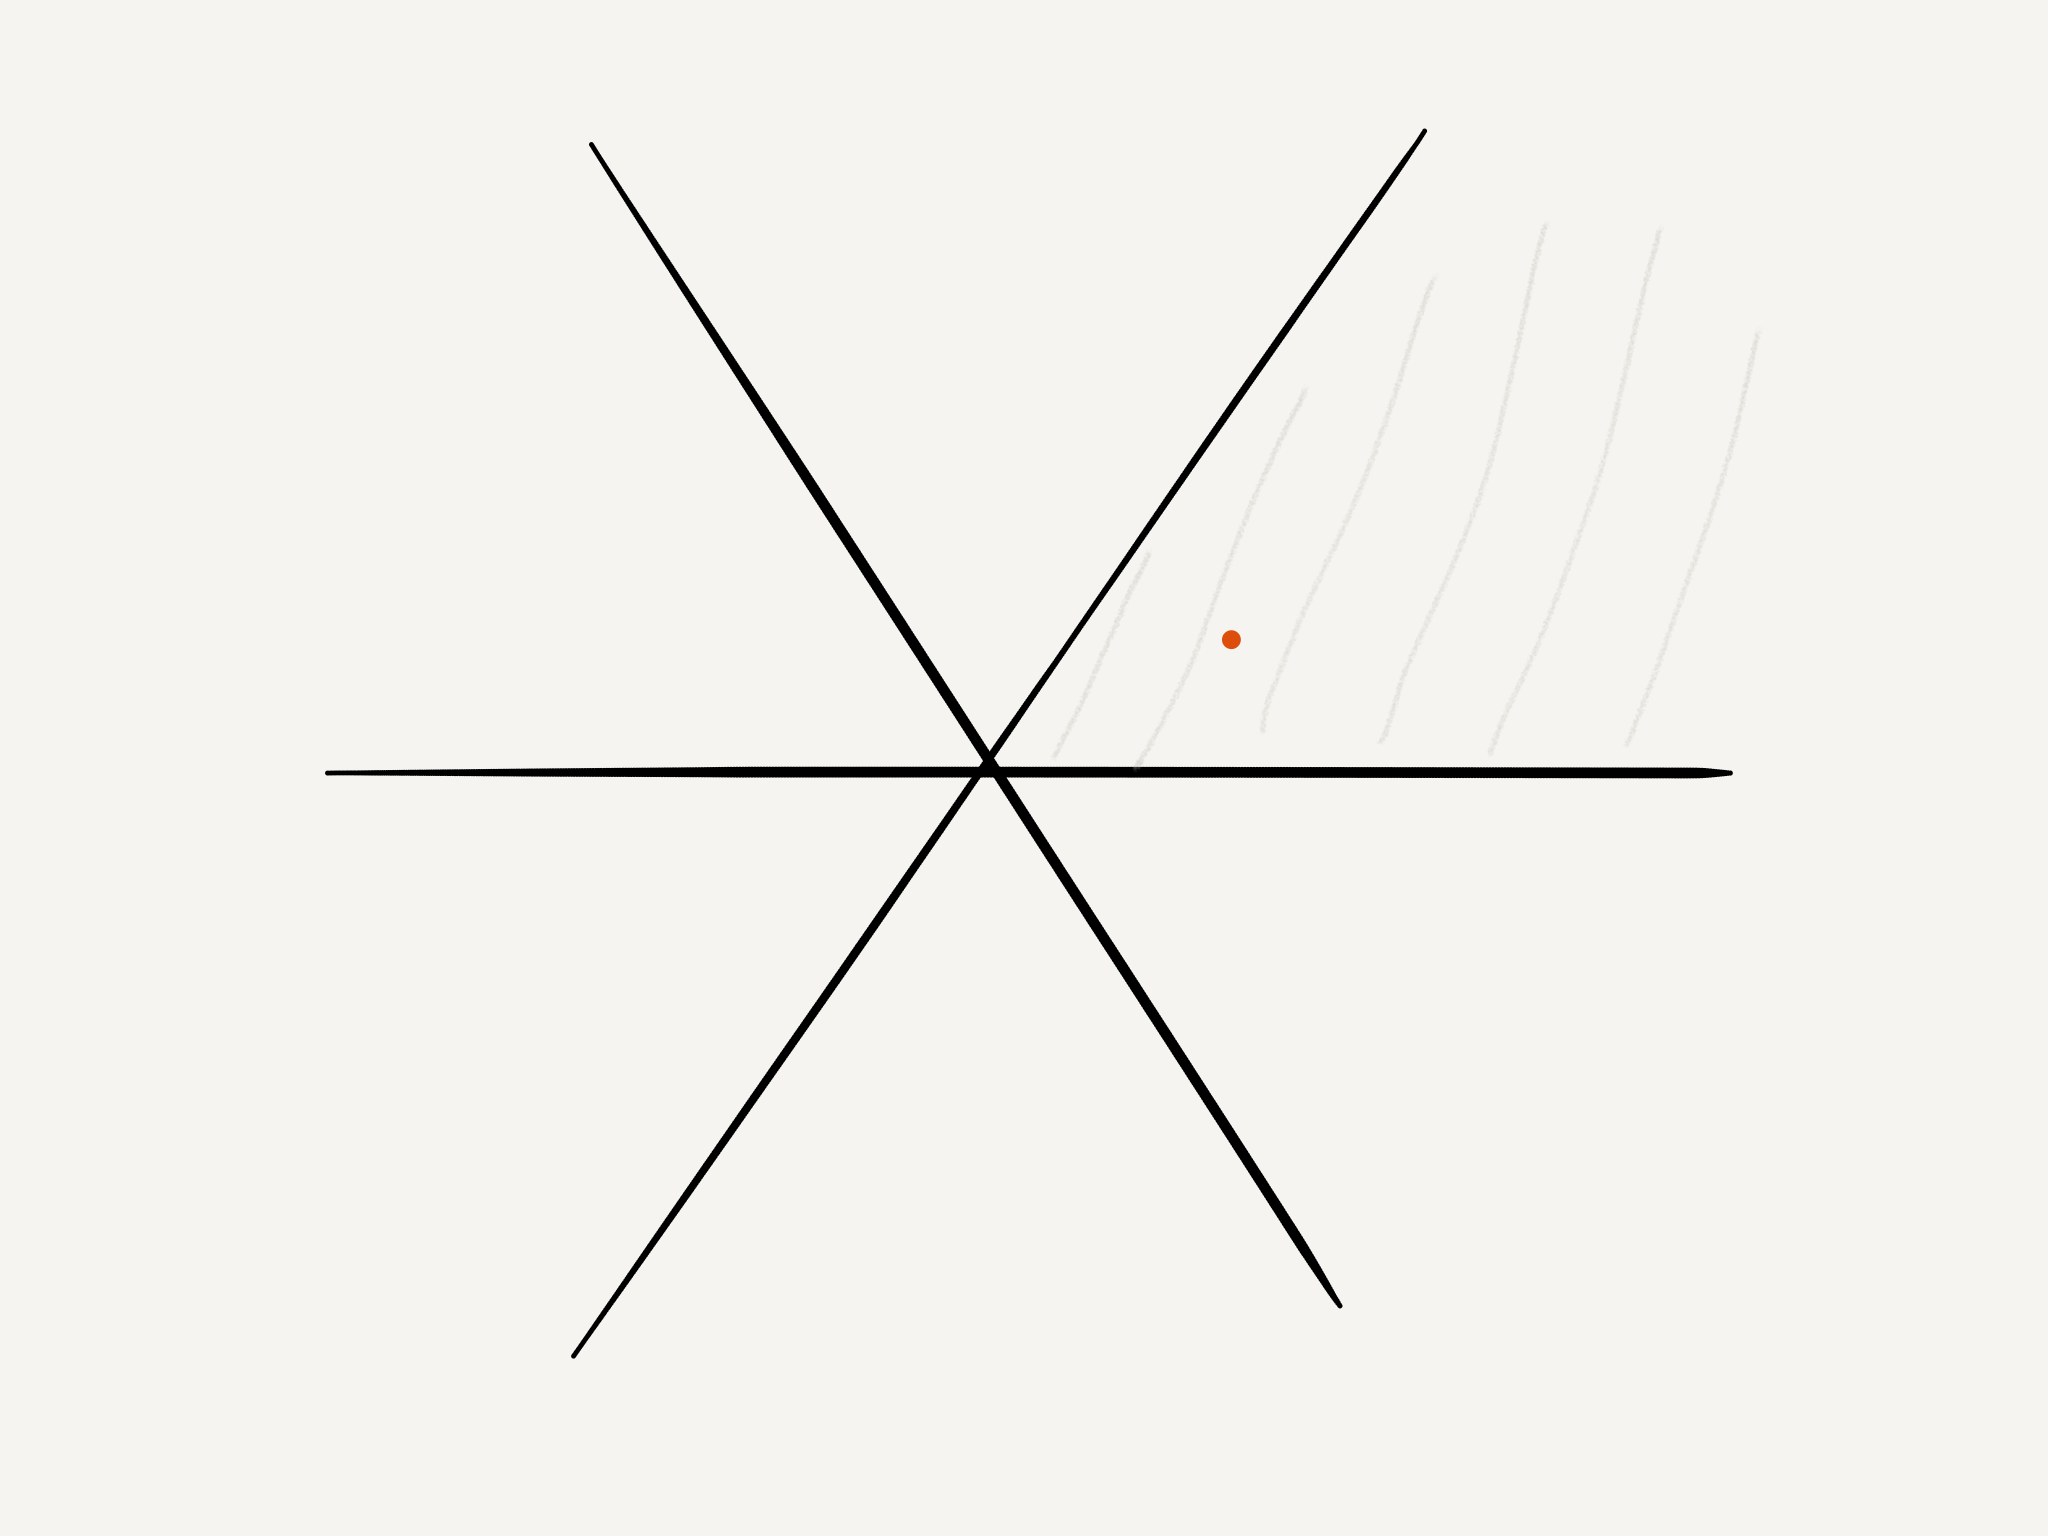
\includegraphics[scale=.25]{249-1}
\caption{A generic coroot lies in the interior of a chamber cut out by the root hyperplanes.} 
\end{figure} 

\begin{remark}
We will see later that if we drop the adjective ``generic'' in Corollary \ref{genborel}
 then we get exactly the parabolic subgroups containing $T$. 
\end{remark}

Choose a generic $\lambda$. Then the decomposition of the Lie algebra under the adjoint action can be grouped as 
\[
\mf{g} = \underbrace{\mf{g}^T}_{\Lie(T)} \oplus \bigoplus_{\substack{a \in \Phi \\ \langle a, \lambda \rangle > 0 }} \mf{g}_a \oplus \bigoplus_{\substack{a \in \Phi \\ \langle a, \lambda  \rangle  < 0 }} \mf{g}_a
\]
Using that $-\Phi = \Phi$, it is easy to thereby deduce that 
\[
\dim B = \frac{1}{2}(\dim G + \dim T).
\]
This is a cute formula for the dimension of the Borel subgroups of a connected reductive group.

\subsection{Quotient of reductive is reductive}

\begin{proposition}\label{torus_centralizes}
If $G$ is connected reductive over a field $k$ and $T \subset G$ is a maximal torus, then $Z_G(T) = T$. 
\end{proposition}

\begin{proof}
We know that $Z_G(T)$ is connected reductive. (This is called a {\em Cartan subgroup}.) But it's a general fact that Cartan subgroups are always solvable! Indeed, $Z_G(T)/T $ is a connected linear algebraic group with no non-trivial tori (the pre-image would be a non-trivial torus not contained in $T$, but $T$ is a \emph{central} maximal torus and in general all maximal tori are conjugate). That implies that $Z_G(T)/T$ is unipotent (22.1.4 of the 
notes for the previous course). In particular $Z_G(T)$ is is solvable. But a connected reductive group is solvable if and only if it's a torus, hence equal to $T$. 
\end{proof}


\begin{lemma}
If $\pi \colon G \twoheadrightarrow G'$ is a surjection of linear algebraic groups, then 
\[
\mathscr{R}_u(G_{\ol{k}}) \twoheadrightarrow \mathscr{R}_u(G'_{\ol{k}}).
\]
In particular, if $G$ is reductive then so is $G'$. 
\end{lemma}

\begin{proof}
First a couple of reductions. Obviously we can assume without loss of generality that $k = \ol{k}$. Because $\pi(\mathscr{R}_u(G)) \subset \mathscr{R}_u(G')$ is normal in $G'$ (as $\pi$ is surjective), 
we can replace $G$ by $G/\mathscr{R}_u(G)$ and $G'$ by $G'/\pi(\mathscr{R}_u(G))$ to assume that $G$ is reductive. 

Let $U' = \mathscr{R}_u(G')$. Then $\pi^{-1}(U')_{\red}^0$ is normal in $G$ (easy exercise) and hence reductive (as we have
already reviewed in the proof of Lemma \ref{quot_cent_red}
the elementary fact that a normal linear algebraic subgroup in a reductive group
is reductive).  Thus, replacing $G'$ with $U'$ and replacing $G$ with $N$
 allows us to assume without loss of generality
that $G'$ is unipotent, and then we want to show that $G'=1$. Let $T \subset G$ be a maximal
torus, so $Z_G(T)  \twoheadrightarrow Z_{G'}(\pi(T)) $ by Corollary \ref{cartan_surj}. But $\pi(T) = 1$ since $G'$ is unipotent, so $Z_{G'}(\pi(T))= G'$. Thus, the unipotent $G'$ is the image of $Z_G(T)= T$ 
(see Proposition \ref{torus_centralizes}), so $G'=1$.
\end{proof}



\section{Central isogeny decomposition}
\subsection{Perfect groups}
Recall that $\SL_2(k)$ is a \emph{perfect group} (meaning that it is own commutator subgroup) for any field $k$ with $\# k >3$. In particular, $\SL_2 = \Cal{D}(\SL_2)$ over \emph{any} field, since this property can be checked on geometric points. 

The group ${\text{SL}}_n$ contains many embedded copies of $\SL_2$:
\[
\SL_n \supset H_{i<j} := \begin{pmatrix} 1 & \\ 
& \ddots \\
& & t_i & \ldots &  x_{ij} \\ 
& & \vdots & \ddots & \vdots \\
& & x_{ji} &  \ldots & t_i^{-1} & \\
& & & & & \ddots \end{pmatrix}
\]
The standard tori $\G_m \subset H_{i<j}$ generate the diagonal torus of $\SL_n$, which implies that the $H_{i<j}$ generate $\SL_n$.

\begin{exercise}
Prove this. [Hint: Consider the open cell $U^- \times T \times U^+ \subset \SL_n$, which is evidently contained in 
the subgroup generated by the $H_{i<j}$.]
\end{exercise}

\begin{lemma}
 $\SL_n$ is perfect. 
\end{lemma}

\begin{example}
For $G = \GL_n$, we have an exact sequence of group schemes 
\[
1 \rightarrow \mu_n \xrightarrow{\xi \mapsto (\xi, \xi^{-1}) }\G_m \times \SL_n \rightarrow G \rightarrow 1
\]
obtained from the diagram 
\[
\xymatrix @C=5pc{
1 \ar[r] & \SL_n \ar[r] \ar[drr] & \GL_n \ar[r]^{\det} & \G_m \ar[r] & 1 \\
1 \ar[r] & \G_m  \ar[urr] \ar[r]_{\text{maximal central torus}} & \GL_n \ar[r] & \PGL_n \ar[r] & 1
}
\]
The diagonal arrows are isogenies, namely the natural quotient map ${\text{SL}}_n \rightarrow {\text{PGL}}_n$
and the endomorphism $t \mapsto t^n$ of $\mathbf{G}_m$.  In particular, it follows that
$\mathscr{D}(\GL_n) = \SL_n$. 

We'll see that this isogeny decomposition for $\GL_n$ adapts to \emph{any} connected reductive 
$k$-group $G$ and that moreover $\Cal{D}G$ is always perfect for such $G$
(and $\mathscr{D}G$ is certainly reductive, since it is normal in $G$). The upshot is that the essential case for most work is perfect connected reductive $G$ (we'll see next time that this is the same as connected semisimple). 
\end{example}

\begin{proposition}
If $G$ is a connected reductive group over $k$, then $\Cal{D}G $ is perfect.
\end{proposition}

\begin{example}
Here is an example to illustrate that connectedness needs to be respected. 
Let $H = \Z/2\Z \ltimes \G_m$, with the $\Z/2\Z$ acting by inversion on $\G_m$. This is clearly reductive. 
Since $(1,t) t (1,t)^{-1} t^{-1}  = t^{-2}$, we have $\G_m \subset \Cal{D}(H)$, and this is an equality
since $H/\G_m$ is commutative. Hence, the derived group is not perfect since it is commutative and
nontrivial. 
\end{example}

\begin{proof}
Let $N = \Cal{D}G \subset G$. This is a characteristic subgroup; i.e. stable under all automorphisms. So its own derived subgroup is still normal (and even characteristic) in $G$: $\Cal{D}^2 G \triangleleft G$. Consider the 
resulting exact sequence 
\[
1 \rightarrow N/\Cal{D}N \rightarrow G/\Cal{D}^2 G \rightarrow G/N \rightarrow 1.
\]
Now, $G/N$ is commutative connected reductive, hence a torus. Since $N$ is normal in $G$ it is also reductive, and connected because the derived subgroup of a connected group is connected, so $N/\Cal{D}(N)$ is also a torus. But then $G/\Cal{D}^2(G)$ is an extension of a torus by a torus, hence is also a torus (by considerations of Jordan decomposition), hence is commutative. Therefore, $\Cal{D}(G/\Cal{D}^2G)$ is its own derived group is trivial, but this is $\Cal{D}G/\Cal{D}^2G$. 
\end{proof}

\subsection{Central isogeny decomposition}\label{zisog}
Classically, for a linear algebraic $k$-subgroup $H$ of
a linear algebraic $k$-group $G$, 
the centralizer was built over an algebraic closure to be smooth (i.e., one made $Z_{G_{\overline{k}}}(H_{\overline{k}})$ as a reduced Zariski-closed subgroup of $G_{\ol{k}}$), 
but it was not clear that this had the expected Lie algebra
$\mathfrak{g}_{\ol{k}}^{H_{\ol{k}}}$, and even less clear whether or not it descends
to a $k$-subgroup of $G$ (but classically for $H$ smooth of multiplicative
type such descent is proved after some hard work).

We shall need the centralizer $Z_G(H)$ as a scheme over the ground field representing
a centralizer functor without 
smoothness hypotheses  on $H$; see Exercise 3(iii) in HW3 of
the previous course for the case of smooth $H$ with no smoothness hypotheses on $G$.  
By using $k$-bases of coordinate rings, one can prove such existence results for 
$Z_G(H)$ and identify its Lie algebra with $\mathfrak{g}^H$
without any smoothness hypotheses; this will be essential later
in this course with smooth $G$ but $H$ a possibly non-smooth $k$-subgroup scheme of a torus
(such as the kernel of a root).  See Exercise 4 in HW7 of the previous course 
for the determination of ${\rm{Lie}}(Z_G(H))$ when $G$ and $H$ are smooth.

Later (via Appendix \ref{Zmucent}) we will take up a proof of the existence of $Z_G(H)$
and the identification of its Lie algebra for 
any affine $k$-group scheme $G$ and closed $k$-subgroup scheme
$H$, by using $k$-bases of coordinate rings in place of the Galois-theoretic
method that works in the smooth case.  If 
$H$ has completely reducible representation theory on finite-dimensional $k$-vector spaces
(e.g., a $k$-group scheme of multiplicative type, such as $\mu_n$, without any smoothness
hypotheses!) then $Z_G(H)$ is also {\em smooth} whenever $G$ is smooth due to 
the infinitesimal criterion
(as presented in Exercise 3 of HW8 of the previous
course when $H$ is a torus). 

\begin{remark}
In HW3 Exercises 3 and 4 of the previous course, for any linear algebraic $k$-group $H$
we built the \emph{scheme-theoretic} center $Z_H \subset H$, as a
closed $k$-subgroup scheme representing the functor on $k$-algebras 
\[
R \rightsquigarrow \{ h \in H(R) \mid \text{conjugation by $h$ is trivial on $H_R$}\}.
\]
From this definition it is clear that $(Z_H)_K = Z_{(H_K)}$ for any $K/k$, but $\Lie(Z_H) \subset \mf{h}$ is a mystery. For instance, $\Lie(Z_{\SL_p}) = \Lie(\mu_p) \neq 0$ inside $\mf{sl}_p$ if $p = \ch k > 0$. 
\end{remark}

\begin{theorem}
Let $G$ be a connected reductive group over $k$ and $Z \subset G$ the maximal central $k$-torus. 
\begin{enumerate}
\item $Z = (Z_G)^0_{\rm{red}}$ and for all $K/k$, $Z_K \subset G_K$ is the maximal central $K$-torus. 

 
 \item The multiplication homomorphism
 $m: Z \times \Cal{D}(G) \rightarrow G$ is a central isogeny $($i.e. an isogeny with central kernel$)$.
 

\end{enumerate}
\end{theorem}

\begin{remark}
\begin{enumerate}
\item[(i)]  In general, for an affine $k$-group scheme $H$ of finite type, 
the underlying reduced scheme 
$H_{\red} \subset H$ can \emph{fail} to be a $k$-subgroup scheme when $k$ is imperfect. 
A \emph{connected} counterexample is given in \cite[VI$_{\text{A}}$, 1.3.2]{SGA3}.
A much easier disconnected counterexample is the $p$-torsion of a Tate curve over a local function field
of characteristic $p$ when the Tate $q$-parameter is not a $p$th power.


\item[(ii)]  This Theorem easily implies that $Z \rightarrow G/\Cal{D}(G)$ and $\Cal{D}G \rightarrow G/Z$ are central isogenies. For $G=\GL_n$, the first map is $t \mapsto t^n$ and the second is $\SL_n \rightarrow \PGL_n$. 
The centrality of kernels of isogenies is automatic in characteristic 0
because a finite group scheme in characteristic 0 is \'etale
and if $H$ is a {\em connected} linear algebraic group over $k$ with any characteristic
then every finite normal {\em \'etale} $k$-subgroup $N$ in $H$ is central 
(much as a discrete normal subgroup of a connected Lie group is central):
conjugation of $H$ on $N$ is classified by a map $H \rightarrow \Aut_{N/k}$,
 and the latter group is finite \'{e}tale, so this classifying map must be trivial. 
 
By contrast, isogenies in characteristic $p$ can have non-central
kernel:  the relative Frobenius isogeny $F_{H/k}:H \rightarrow H^{(p)}$
for a linear algebraic group $H$, whose infinitesimal kernel $N \subset H$ has full Lie algebra
(very non-commutative when $H = {\text{SL}}_n$ with $n > 1$, for example).
\end{enumerate}
\end{remark}

\begin{proof}
For (1), let $T \subset G$ be a maximal $k$-torus. Then $T = Z_G(T)$ by Lemma \ref{torus_centralizes}, hence contains $Z_G$. It is a general fact that for \emph{tori}, the underlying reduced scheme is always a subgroup
whose formation commutes with extension of the ground field. 
More specifically for our purposes, 
for any closed $k$-subgroup $M \subset T$, $M_{\red}$ is a $k$-subgroup whose formation commutes with extension of $k$ [for a proof, see Lemma \ref{tored}]. (The idea of the proof is that you can pass to the separable closure, and so assume that $k=k_s$, so $T$ splits as $\G_m^r$. Then the subgroups of $T$ correspond to quotients of the character group, i.e. $M = \ul{\Hom}(\Lambda, \G_m)$ for some quotient $\Lambda$ of $\Z^r$. But by the structure of $\G_m$, $M$ is necessarily of the form $\G_m^s \times \prod \mu_{\ell_i^{e_i}}$ for some primes $\ell_i$, so it reduces to the fact that $(\mu_{p^{e}})_{\red}=1$ if $p= \ch k >0$.)

This shows that $(Z_G)_{\red}^0$ is a torus, but $Z \subset (Z_G)_{\red}^0$ by definition, so we must have $Z = (Z_G)_{\red}^0$. Since $(Z_G)_{\red}^0$ commutes with formation of extension on $k$ (by the preceding discussion plus the fact that the formation of $Z_G$ and of identity components of group schemes
of finite type each commute with extension of the ground field), $Z$ does too. \\

(2) Let's first show that $\ker m$ is central and finite. The centrality is easy: the kernel is $Z \cap \Cal{D} G \hookrightarrow Z \times \Cal{D} G$ embedded via $(t,t^{-1})$, and anything intersected with $Z$ is obviously central.

For finiteness, we use:

\begin{lemma}
Let $H$ be a connected linear algebraic group over $k$ and $C \subset H$ a central 
$k$-torus. Then $C \cap \Cal{D}(H)$ is finite.
\end{lemma}

\begin{proof}
The idea is to reduce to the case $H = \GL_n$. Without loss of generality,
$k = \ol{k}$. Choose a closed immersion $H \hookrightarrow \GL(V)$
as $k$-groups. Under the $C$-action on $V$ we get a weight space decomposition
\[
V = \bigoplus_{\chi \in {\rm{X}}(C)} V_{\chi}.
\]
Since $C \subset H$ is central, the $H$-action on $V$ preserves the $C$-eigenspaces, so we get an embedding $H \hookrightarrow \prod \GL(V_{\chi})$ under which $C \hookrightarrow \prod_{\chi} \G_m$. But $\Cal{D}(H) \subset \prod_{\chi} \SL(V_{\chi})$, so it is enough to observe that $\G_m \cap \SL_n = \mu_n$ is finite for any
$n \ge 1$. 
\end{proof}

Finally, we show the surjectivity of $m \colon Z \times \Cal{D} G \rightarrow G$. It is the same to show that $G/Z$ is perfect. But $G/Z$ is connected reductive with trivial maximal central torus, since a \emph{normal} torus $S$ inside a connected linear algebraic group $H$ is always central (by Exercise 3 of HW6 of the previous course:
conjugation on $S$ is classified by a  homomorphism $H \rightarrow \Aut_{S/k}$  whose target is
 \'{e}tale; e.g. if $S$ is split, then this
automorphism scheme is the constant group $\GL_n(\Z)$). The upshot is that by replacing $G$ with $G/Z$, we can reduce to the case where $Z$ is trivial, and then we want to show that $G$ is perfect. 


Without loss of generality we may assume that $k = \ol{k}$, so all $k$-tori are split.
Let $T$ be a maximal torus in $G$. For $a \in \Phi(G,T)$, recall that we defined a 
smooth connected subgroup $G_a := Z_G(T_a) \subset G$ where $T_a = (\ker a)^0_{\red}$
and $G_a/T_a \simeq \SL_2$ or $\PGL_2$.
In particular, $G_a/T_a$ is perfect, so the multiplicative homomorphism
$$T_a \times \mathscr{D}(G_a) \rightarrow G_a$$
with finite central kernel is {\em surjective} too; i.e., for $G_a$ (with maximal
central torus $T_a$ of codimension 1 in the non-central maximal torus
$T \subset G_a$) the desired central-isogeny result
is known to hold. 
Moreover, we saw via dynamic considerations with $U(\pm \lambda)$
for suitable $\lambda \in {\rm{X}}_{\ast}(T)$ that the $T$-equivariant 
map $\Cal{D}(G_a) \rightarrow G_a/T_a$ induces an isomorphism on the 
$T$-weight spaces for nontrivial weights, so the Lie algebra of $\Cal{D}(G_a)$ has $a$ as a 
$T$-weight.  

Since $T = Z_G(T)$ has Lie algebra $\mf{g}^T$, 
it follows that ${\text{Lie}}(G)$ is spanned by the Lie algebras of $T$
and the $\mathscr{D}(G_a)$'s (using all roots $a$).
Thus, the connected linear algebraic
subgroup $\langle T, \Cal{D}(G_a) \rangle_{a \in \Phi} \rangle $ has full Lie algebra, so it is equal to $G$. 
So far we have not used the triviality hypotheses on $Z$.

Now it suffices to show that $T \subset \Cal{D}G$ when $Z=1$. This 
is immediate from the following claim. 

\end{proof}


\begin{proposition} If $Z=1$ then $T = [T, N_G(T)]$. 
\end{proposition}

\begin{proof} Of course the containment $\supset $ is trivial because $tnt^{-1}n^{-1} = t(ntn^{-1}) \in T$. The substance is in the other direction. 

Recall the Weyl group $W = N_G(T)/Z_G(T) = N_G(T)/T$, which is {\em finite}
(see Exercise 4 in HW6 of the previous course). We consider the map
 \[
 T \rtimes N_G(T) \rightarrow G.
 \]
 For $w \in W$ represented by $n \in N_G(T)$, we have 
\[
ntn^{-1}t^{-1} = (ntn^{-1})t^{-1} = (w \cdot t)/t.
\]
We want to show that $T$ is generated by commutators, and this shows that $(w \cdot t)/t$ is a commutator. So it suffices to show that $T$ is generated by elements of the form $(w \cdot t)/t$.  

To this end, consider the subtorus  
\[
S_w = \Ima(T \xrightarrow{t \mapsto (w \cdot t)/t} T).
\]
It's enough to show that the $S_w$ generate $T$. We can check this by showing that any character $\chi \in {\rm{X}}(T)$ which is trivial on each $S_w$ must be trivial on all of $T$, i.e. if $\chi|_{S_w}=1$ for all $w$ then $\chi =1$. The condition that $\chi|_{S_w}=1$ is simply that $\chi(t) = \chi(w \cdot t)$ for all $t \in T$, i.e. $\chi \in \chi(T)^w$. So it is equivalent to show that ${\rm{X}}(T)_{\Q}^W = 0$. 

The reason for passing to rational coefficients is that we have a good theory of representations of finite groups 
(such as $W$) over fields of characteristic 0 (such as $\Q$). For instance we know that $\Q[W]$-modules are semisimple, so ${\rm{X}}(T)_{\Q}^W= 0 $ if and only if the \emph{dual} module has trivial $W$-invariants. The dual is the familiar object ${\rm{X}}_*(T)_{\Q}$, so we have reduced to showing that ${\rm{X}}_*(T)^W = 0$. 

Now this is a more concrete statement, since ${\rm{X}}_*(T) = \Hom(\G_m, T^W)$. This is equivalent to $T^W$ having no non-trivial subtori, but to say that a closed subgroup scheme $M$ of a torus
contains no non-trivial subtori is to say that $M$ is finite. So we have reduced to showing that 
$T^W$ is finite when $Z=1$. 

\begin{example}
Consider $G = \GL_n$ versus $G = \SL_n$. Take $T$ to be the diagonal torus in either case, so $W = S_n$
via coordinate permutation. What is $T^W$? It is the group of scalar matrices (since $W$ acts by permutation on the  coordinates). So $T^W $ is $\mu_n$ for $\SL_n$ and $\G_m$ for $\GL_n$.  Note
that $Z = 1$ for $\SL_n$, but $Z \ne 1$ for $\GL_n$.
\end{example}

\begin{lemma}
If $Z=1$, then $\bigcap_{a \in \Phi} \ker (n_a   a) $ is finite for any collection of $n_a \in \Z-\{0\}$. 
\end{lemma}

(The converse is obviously true). 

\begin{proof}
Since a closed subgroup scheme $M$ of a torus contains a torus if and only if $M$ is  not finite
(as $M^0_{\rm{red}}$ is a torus), 
it is the same to show that if a subtorus 
$S \subset T$ is killed by all characters $n_a a$, then $S=1$. Consider the restriction map 
\[
{\rm{X}}(T) \rightarrow {\rm{X}}(S)
\]
and note that ${\rm{X}}(S)$ is torsion-free (since $S \xrightarrow{t^n} S$ is surjective for all $n \neq 0$). Therefore 
\begin{align*}
n_a \cdot a|_S =1 & \iff a|_S = 1 \\
& \iff \mf{g}^S \supset \mf{g}_a \\
&\iff \Lie(Z_G(S)) \supset \mf{g}_a.
\end{align*}
Certainly $Z_G(S) \supset Z_G(T)$, so $\Lie(Z_G(S)) \supset \Lie(Z_G(T)) \supset \mf{g}^T$. But then $\Lie(Z_G(S))$ contains $\mf{g}^T$ \emph{and} all the root lines, so $\Lie( Z_G(S)) \supset \mf{g}^T \oplus \left( \bigoplus_{a \in \Phi} \mf{g}_a \right) = \mf{g}$, so $Z_G(S) \subset G$ as a connected smooth subgroup is full, i.e. $S \subset Z_G$. The assumption $Z=1$ obviously finishes off the proof, but notice that none of the preceding argument required that hypothesis. 
\end{proof}

Now the proof is (finally!) completed by the following general Lemma (which requires no hypotheses on $Z$). \end{proof}

\begin{lemma}
We have $T^W \subset \ker (2a)$ for all $a \in \Phi = \Phi(G,T)$.
\end{lemma}

\begin{proof}
Choose $a$ and consider $G_a = Z_G(T_a)$ for $T_a = (\ker a)^0_{\red} \subset T$. We're going to use a special case of the theorem (which we're trying to prove) that we already know:  the map 
\[
\pi_a \colon T_a \times \Cal{D}(G_a) \rightarrow G_a
\]
is a central isogeny, because $G_a/T_a$ is perfect (since it's $\SL_2$ or $\PGL_2$). 

\begin{remark} Since $\Cal{D}(G_a) \rightarrow G_a/T_a = \SL_2$ or $\PGL_2$ is a central isogeny, it follows that $\Cal{D}(G_a) $ has rank one and is not solvable (being perfect), so is either $\SL_2$ or $\PGL_2$. 
\end{remark}

\begin{remark}
It is shown in Example \ref{redssex} that 
for $\PGL_n$, $n \geq 3$ we always have $\Cal{D}(G_a) = \SL_2$
whereas for $\SO_5$ we sometimes gets $\SL_2$ and sometimes get $\PGL_2$ (depending on $a$). 
\end{remark}

We want to reduce to the rank-1 case. Note that for any \emph{central} quotient map $f \colon H \twoheadrightarrow H'$ (i.e. a quotient by central subgroup scheme) between
 connected reductive groups over an {\em arbitrary} field $k$, it is always the case that there is a bijection 
\[
\{\text{maximal $k$-tori of $H$}\} \Longleftrightarrow \{ \text{maximal $k$-tori of $H'$}\}
\]
which is given explicitly by $f \mapsto f(T)$ and $f^{-1}T' \mapsfrom T'$ (using
scheme-theoretic preimage, as always). Why? To prove the recipes give maximal $k$-tori
(e.g., that $f^{-1}(T')$ is $k$-smooth) and are inverse to each other, it suffices to check after
an extension on $k$; hence, we may and do assume $k = \ol{k}$.
Thus, all maximal tori are conjugate, so we just have to show that the (scheme-theoretic) 
preimage of one maximal torus is a maximal torus. Start with a maximal torus $T$ in $H$, and we want to know if it is the full preimage of its image. In other words, we need to know that $T$ contains the kernel, and this follows from $\ker f$ being central since $Z_H \subset Z_H(T) = T$. 

Apply this discussion to $f = \pi_a$. Then $\pi^{-1}(T)$ is a maximal torus in $T_a \times \Cal{D}(G_a)$. What can we say about this maximal torus? It contains $T_a$, since the maximal torus 
in a direct product of linear algebraic groups
is a direct product of maximal tori in the factors (as
we may check after passage to an algebraically closed field and using conjugacy considerations),
 so $\pi_a^{-1}(T) = T_a \times \Cal{T}_a$ for $\Cal{T}_a = T \cap \Cal{D}(G_a)$. Thus,
 $\Cal{T}_a$ is a 1-dimensional torus (in particular, smooth and connected!). 
 
 Note that 
\[
T_a \times \Cal{T}_a \rightarrow T
\]
is an isogeny, with $T_a$ central in $G_a$, so it induces an isomorphism of the rational character groups:
\[
{\rm{X}}(T_a)_{\Q} \oplus {\rm{X}}(\Cal{T}_a)_{\Q} \xleftarrow{\sim} {\rm{X}}(T)_{\Q}.
\]
The whole game is to produce elements of the Weyl group that visibly cut down the invariant space. We know that 
\[
(\Cal{D}(G_a), \Cal{T}_a) \simeq (\SL_2 \text{ or } \PGL_2, \text{diagonal torus})
\]
so we have an element $n_a = \begin{pmatrix} 0 & 1 \\ -1 & 0 \end{pmatrix} \in N_{G(a)}(\Cal{T}_a)$. Note that $n_a \in N_G(T_a \cdot \Cal{T}_a) = N_G(T)$ since it centralizes $T_a$ and also normalizes $\Cal{T}_a$, which together generate $T$, and so represents an element $w_a \in W$. We'll show that $T^{w_a} \subset \ker (2a)$,
which will do the job.

Look at the decomposition
\[
{\rm{X}}(T)_{\Q} = {\rm{X}}(T_a) \oplus {\rm{X}}(\Cal{T}_a)_{\Q}.
\]
The first summand is a hyperplane and the second summand is a line. What does $w_a$ do? It restricts to the identity on the hyperplane, and negation on the line by inspection. This is a reflection (by definition, an automorphism which is the identity on a hyperplane and negation on the quotient line). We claim that the following diagram commutes:
\[
\xymatrix{
T \ar[r]^{a} \ar[d]_{n_a\text{-conj}}  & \G_m \ar[d]^{-1} \\
T \ar[r]_{a} & \G_m 
}
\]
It suffices to check this on $T_a, \Cal{T}_a$ separately. On $T_a$, the compositions are both trivial. 
On $\Cal{T}_a$, they are both $-a$. 

Now, suppose that you have a fixed point $t \in T^W$. Then commutativity of the diagram
gives that $a(t)=1/a(t)$, so one has 
\[
a(t)^2 [=t^{2a}] = 1
\]
as desired (by definition of the notation $2a \in {\rm{X}}(T)$).
\end{proof}



\begin{lemma}
For $G $ connected reductive and perfect
and a split maximal torus $T \subset G$, $\Z \Phi \subset {\rm{X}}(T)$ has finite index. 
\end{lemma}

\begin{proof}
We always have the central isogeny 
\[
Z \times \Cal{D}G \rightarrow G
\]
so $G = \Cal{D}G \iff Z=1$. On the other hand, $\Z \Phi$ has finite index in $ {\rm{X}}(T)$ if and only if $\bigcap_{a \in \Phi} \ker a $ contains no $\G_m$ (this is an easy exercise concerning the relationship between subtori and quotient lattices), which as seen above is equivalent to $Z=1$. 
\end{proof}

\begin{lemma}
Let $G$ be a connected linear algebraic group over a field $k$. Then the following are equivalent: 
\begin{enumerate}
\item the geometric solvable radical $\mathscr{R}(G_{\ol{k}})$ is trivial $($the definition of semisimplicity!$)$;
\item $G$ is reductive and $Z = 1$;
\item $G$ is reductive and perfect.
\end{enumerate}
\end{lemma}

\begin{proof}
The equivalence of (2) and (3) is clear from central isogeny decomposition. 

For the equivalence of (1) and (2), the point is that we know that the formation of $Z$ is compatible with base change, so we can assume that $k = \ol{k}$. Being central and solvable, $Z$ is always in the solvable radical. Conversely, a normal connected solvable subgroup in a connected reductive group is a
normal torus (as it is a solvable connected reductive group, hence a torus) and this is central torus
(as normal tori in connected linear algebraic groups are always central, due to \'etaleness of the automorphism
scheme of a torus).
\end{proof}


All the real work in representation theory is in the semisimple case, but 
for inductive purposes it's better to work in the reductive setting because one wants to make constructions, e.g. torus centralizers, which pass out of the semisimple realm. 

\subsection{Applications}\label{tbcentral}
For any {\em central} isogeny $G \twoheadrightarrow G'$ 
(or more generally central quotient map) between
 connected reductive groups over \emph{any} field $k$, we have seen that there is a natural bijection 
\[
\{\text{maximal tori of $H$}\} \Longleftrightarrow \{ \text{maximal tori of $H'$}\}
\]
given by 
\begin{align*}
T & \mapsto f(T) \\
f^{-1}(T') & \mapsfrom T'.
\end{align*}
The same applies for parabolic $k$-subgroups, as well as
for Borel $k$-subgroups (if any exist!), by the same argument. 

Apply this to $Z \times \Cal{D} G \rightarrow G$ for connected 
reductive $G$ over a field $k$ to obtain that the set of
maximal $k$-tori of $\Cal{D}G$ is in bijection with the set of maximal $k$-tori of $G$ via the constructions
\begin{align*}
\mathscr{T} & \mapsto Z \cdot \mathscr{T} \\
T \cap \Cal{D} G & \mapsfrom T
\end{align*}
and likewise for parabolics $k$-subgroups and Borel $k$-subgroups.   We emphasize
that these bijections work with $k$-subgroups; e.g., $G$ contains a Borel $k$-subgroup
if and only if $\Cal{D}G$ does.

\begin{example}
This fails without the centrality assumption. Example \ref{cftex} show 
that such a counterexample over any local function field $k$ of characteristic $p>0$ is given by 
the non-central isogeny $f:\underline{D}^{\times} \rightarrow \GL_p$ 
arising from the relative Frobenius isogeny for $\underline{D}^{\times}$ where
$D$ is a central division algebra of dimension $p^2$ over $k$.  (If $T \subset \GL_p$
is a split maximal $k$-torus then $f^{-1}(T)$ is a {\em non-smooth} $k$-subgroup scheme of
$\underline{D}^{\times}$, and 
$f^{-1}(T)_{\rm{red}}$ is {\em not} a smooth $k$-subgroup scheme of $\underline{D}^{\times}$;
the same goes for a Borel $k$-subgroup of $\GL_p$.) 

The key point is that 
$\underline{D}^{\times}$ has no Borel $k$-subgroup nor a split maximal 
$k$-torus due to $D$ being a central division algebra, and
$D$ is split by any degree-$p$ extension (such as the $p$-power endomorphism $k \rightarrow k$) due to 
local class field theory.  (The invariant of a central simple algebra multiplies by $d$ under a degree-$d$ extension, so a central division algebra with invariant $j/p \in \Q/\Z$ splits after a degree-$p$ extension.)  It
is this latter splitting that allows us to identify the Frobenius base change of $\underline{D}^{\times}$
with $\GL_p$. 
\end{example}

\subsection{Central isogenies preserve roots}
The central isogeny decomposition shows that up to central isogeny, for problems with connected reductive $k$-groups $G$ it is often sufficient to examine $\Cal{D}G$, which has the advantage of being semisimple. (This applies, for instance, in studying problems involving maximal $k$-tori, or Borel $k$-subgroups, and so on.)
Here is another instance of the same principle:

\begin{proposition}\label{central_isog_roots}
For a central isogeny $f \colon G \rightarrow G'$ of connected reductive $k$-groups, and $T \subset G$ a split maximal $k$-torus with $T' = f(T') \subset G'$ $($necessarily also split maximal$)$, under the inclusion ${\rm{X}}(f) \colon {\rm{X}}(T') \hookrightarrow {\rm{X}}(T)$ the set of roots $\Phi' := \Phi(G', T')$ are mapped bijectively to $\Phi(G,T) =: \Phi$.
\end{proposition}

(We need a split maximal torus to have a weight space decomposition. The formation of weight space decomposition commutes with field extension, so the facts we know about root spaces over algebraically closed fields, such as 1-dimensionality and $\Phi \cap \Q \cdot a = \{\pm a\}$, apply over $k$.) 

Before proving this result, we make some general observations.

\begin{remark}This is only interesting in characteristic $p$ since it is trivial when
$f$ is \'etale (as then ${\text{Lie}}(f)$ is an isomorphism). 
If $f$ is not \'{e}tale (e.g. $\SL_p \rightarrow \PGL_p$) then the finite group scheme
$\ker f$ must hae nonzero Lie algebra, so $\mf{g} \rightarrow \mf{g}'$ is not injective
and hence is not surjective (as $G$ and $G'$ have the same dimension).
This failure of surjectivity is what gives the result some substance,
as it is not clear a priori that a root line in the target is in the image of ${\text{Lie}}(f)$. The proof
will show that it is in the image (of a unique root line in the source).
\end{remark}

\begin{remark}\label{centralrem}
Apply this result to the central isogeny 
\[
Z \times \Cal{D}G \rightarrow G.
\]
If $T \subset G$ is a split maximal torus, then it pulls back to a split maximal torus of the form $Z \times \Cal{T} \subset Z \times \Cal{D}G $. This induces a finite-index inclusion 
\[
{\rm{X}}(T) \hookrightarrow  {\rm{X}}(Z) \oplus {\rm{X}}(\Cal{T}).
\]
Clearly $\Phi(G,T)$ restricts to $0$ on ${\rm{X}}(Z)$, so must map bijectively to $\Phi(\Cal{D}G, \Cal{T})$. In other words, every root of the derived group arises from a unique root of the ambient group. Informally,
this says that the root system of $G$ only knows $\Cal{D}G$. (The roots also only know about $G$ up to central isogeny, which is why one needs to keep track of a {\em root datum} in the classification up to isomorphism.) 
\end{remark}

\begin{exercise}
Centrality is crucial! For the relative Frobenius isogeny $F_{G/k} \colon G \rightarrow G^{(p)}$ 
in characteristic $p$ 
(e.g. $\SL_n \rightarrow \SL_n$ by $(x_{ij}) \mapsto (x_{ij}^p)$), the effect on the roots is to identify 
${\text{X}}(T^{(p)})$ with $p \cdot {\text{X}}(T)$ and 
$\Phi(G^{(p)}, T^{(p)})$ with $p \Phi(G,T)$.  (Hint: show that the composition of the natural bijection
${\text{X}}(T) \simeq {\text{X}}(T^{(p)})$ induced by base change with 
the pullback map ${\text{X}}(T^{(p)}) \rightarrow {\text{X}}(T)$ is
multiplication by $p$). 
\end{exercise}

\begin{example}
There are even more bizarre examples, coming from exceptional isogenies in low
characteristic such as $\SO_{2n+1} \rightarrow \Sp_{2n}$ in characteristic $2$. 
This has commutative non-central kernel $\alpha_2^{2n}$. When $n=1$, this is $\PGL_2 \rightarrow \SL_2$, which is an instance of the more general disorienting map $\PGL_p
= \SL_p\mu_p \rightarrow \SL_p$ (induced by $F_{\SL_p/k}$) 
from the adjoint type to the simply connected type.
\end{example}


\begin{proof}[Proof of Proposition \ref{central_isog_roots}]
Choose $\lambda \in {\rm{X}}_*(T)$ and let $\lambda' = f \circ \lambda \in {\rm{X}}_*(T')$. Since $f$ induces an isomorphism ${\rm{X}}_*(T)_{\Q} \simeq {\rm{X}}_*(T')_{\Q}$, we can choose the cocharacter $\lambda$ so that \emph{both} $\lambda$ and $\lambda'$ are generic (i.e. lie outside the root hyperplanes). We have the map of open cells
\[
\xymatrix @C=.5pc{
G \ar[d]_f & & & &  U(-\lambda)  \ar@{_{(}->}[llll]  \ar[d] & \times & T \ar[d] & \times & U(\lambda) \ar[d] \\
G' & & & & U(-\lambda') \ar@{_{(}->}[llll]  &  \times & T' & \times & U(\lambda') 
}
\]
Since $\ker f \subset Z_G \subset Z_G(T)=T$, we have $\ker f = \ker (T \rightarrow T')$. So $U(-\lambda) \simeq U(-\lambda')$ and $U(\lambda) \simeq U(\lambda')$. Since the roots are contained in the Lie algebras of these unipotent factors, the result now follows from passing to the map on Lie algebras. 
\end{proof}

\section{Grothendieck's covering theorem}\label{grcover}
\subsection{Statement and proof}
We need one more big theorem before we get into the fine structure theory of reductive groups, which asserts that a linear algebraic group is covered by Borel subgroups, a vast generalization of the statement that any 
$n \times n$ matrix 
over an algebraically closed field can be conjugated to be upper triangular. 

\begin{theorem}[Grothendieck's Covering Theorem]\label{gcover} Let $G$ be a connected linear algebraic group over $k= \ol{k}$. Let $B \subset G$ be a Borel subgroup. Then 
\[
G(k)  = \bigcup_{g \in G(k)} g B(k) g^{-1}. 
\]
\end{theorem}

\begin{remark}
We'll see later that this has \emph{many} useful consequences. For $G = \GL_n$ it is the familiar fact that every matrix can be conjugated to be upper triangular. 
\end{remark}

\noindent \textbf{Outline of proof.}  For a linear algebraic subgroup $H \subset G$, we define 
 \[
 \Sigma_H = \bigcup_{g \in G(k)} gH(k)g^{-1}.
 \]
 
 \emph{Step 1.} We'll show that $\Sigma_B$ is closed in $G(k)$ (for the Zariski topology). \\
 
 \emph{Step 2.} Choose $T \subset B$ a maximal torus (necessarily also maximal in $G$). Then $Z_G(T) \subset B$ (e.g. pass to $G/\mathscr{R}_u(G)$ and use the fact that maximal tori are their own centralizers in connected
 reductive groups) so 
 \[
 \Sigma_{Z_G(T)} \subset \Sigma_B.
 \] 
 We'll show that $\Sigma_{Z_G(T)}$ is \emph{dense} in $G(k)$. (This is like the statement that a random matrix is semisimple with distinct eigenvalues.) \\
 
 
 Now we begin the proof of Theorem \ref{gcover}.
Consider the map 
\[
f_H \colon G \times G \xrightarrow{\mu} G \times G \xrightarrow{p_1 \times 1 } (G/H) \times G = (G \times G)/(H \times 1).
\]
where $\mu$ sends $(g,g') \mapsto (g, gg'g^{-1})$, which is an isomorphism. We track the subgroup $G \times H$:
\[
\xymatrix{
f_H \colon G \times G \ar[r]^{\mu}_{\sim} \ar[r] &  G \times G \ar[r]^{p_1 \times 1 } & (G/H) \times G \\
G \times H \ar@{^{(}->}[u] \ar[r] & \mu(G \times H) \ar[r] \ar@{^{(}->}[u] & f_H(G \times H)\ar@{^{(}->}[u]
}
\]
Now $\mu(G \times H) = \{ (g, ghg^{-1})\}$ which is stable by $H$-translation on the right on the first factor. So the map $\mu(G \times H) \rightarrow f_H(G \times H)$ is a \emph{quotient} map by $H \times 1$. 
In particular, by descent theory for closed subschemes, $f_H(G \times H)$ is closed in
$(G/H) \times G$. 

Note that $p_2 (f_H(G \times H))(k) = \Sigma_H$. So if $G/H$ were proper, then $(G / H) \times G \xrightarrow{p_2} G$ would be closed, hence $\Sigma_H$ would be closed in $G$. 
But that properness holds for $H=B$. This completes Step 1. 

Next, we want to show that $\Sigma_H$ is dense when $H \subset G $ is a Cartan subgroup. 
Working with general $H$, consider the map $\pi$ defined by composing $f_H$ with $p_2$:
\[
\xymatrix{
f_H(G \times H) \ar[r] \ar[dr]_{\pi} & (G/ H) \times G \ar[d]^{p_2} \\
& G
}
\]
which has image $\Sigma_H$ on $k$-points. We want to show that this is dominant, so we should get a handle on the dimension of the source. The map $f_H$ is the composition of $\mu$, which is an isomorphism, with
a quotient by $H \times 1$, so 
\begin{align*}
\dim f_H(G \times H) & = \dim \mu(G \times H) - \dim (H \times 1) \\
&= \dim  G + \dim H - \dim H \\
&= \dim G
\end{align*}
If $\Sigma_H \subset G(k)$ is dense then $\pi$ has finite fibers over a dense open in $G(k)$
(as for any dominant map between varieties of the same dimension). 
Even better, the converse holds with just \emph{one} finite non-empty fiber over $G(k)$, by semicontinuity
for fiber dimension. 

So what is the fiber of $\pi$ over a point $g_0 \in G(k)$? Chasing through the definition, 
\[
\pi^{-1}(g_0) = \{ (gH, g_0) \mid g^{-1} g_0 g \in H\}.
\]
Note that $g^{-1} g_0 g \in H \iff g_0 \in gHg^{-1}$. This is finite if and only if 
$$\{\overline{g} \in G(k)/H(k) \,|\, g_0 \in gHg^{-1}\}$$ is finite. We'd like to massage this a little bit, and replace 
$G/H$ with $G(k)/N_G(H)(k)$. Of course, the condition on $g$ only depends on its right $N_G(H)$-coset,
not just its right $H$-coset, but we have to make sure that the finiteness aspect
of the counting isn't screwed up either. So \emph{if} $H \subset N_G(H)$ has finite index on $k$-points, then we can index by $\ol{g} \in G(k)/N_G(H)(k)$. We claim that this finite-index property holds for Cartan subgroups $H$:

\begin{example} The group
$H := Z_G(T)$ for maximal $T \subset G$ has finite index in $N_G(H)$. Indeed, $T \subset Z_G(T)$ is the \emph{unique} maximal torus in $Z_G(T)$, so any (smooth)
subgroup of $G$ normalizing $Z_G(T)$ must normalize $T$. Hence, 
\[
Z_G(T) = H \subset N_G(H) \subset N_G(T)
\]
but the outer inclusion is finite index on $k$-points!
\end{example}

The upshot is that it is enough to find $g_0$ which lies in only finitely many (and at least one!) Cartan subgroups. 
We will show that most points in a maximal torus $T$ of $G$ lie in a unique Cartan subgroup, namely
$Z_G(T)$; that will finish the proof of Theorem \ref{gcover}.

\begin{definition}
For $T \subset G$, we say that $t \in T(k)$ is \emph{regular} if $a(t) \neq 1$ for all $a \in \Phi(G,T)$. 
\end{definition}


This means that 
\[
t \in T - \left( \bigcup_{a \in \Phi} \ker a \right)
\]
so there are many such $t$. 

\begin{remark}
A priori this definition depends on a choice of $T$, but we will later see that it is in fact an intrinsic property
of a semisimple element $t \in G(k)$.
\end{remark}

\begin{example}
For $G = \GL_n$ and $T$ the diagonal torus, then 
\[
\Phi := \Phi(G, T) = \{ a_{ij} \colon t \mapsto t_i/t_j\}_{i \neq j}
\]
 so $t \in T$ is regular with respect to $T$ if and only if $t$ has distinct eigenvalues. 
\end{example}

\begin{example}
For $G = \SL_2$ and $T$ the diagonal torus 
\[
T = \left\{ \begin{pmatrix} c & \\ & c^{-1} \end{pmatrix} \right\}
\]
the roots are $(\begin{smallmatrix} c & 0 \\ 0 & c^{-1} \end{smallmatrix}) \mapsto c^{\pm 2}$, so regularity is the condition $c^2 \ne 1$.
\end{example}

\begin{example} For $ G = \PGL_2$ and $T$ the diagonal torus 
\[
T = \left\{  \begin{pmatrix} c & \\ & 1 \end{pmatrix} \right\}
\]
the roots are $(\begin{smallmatrix} c & 0 \\ 0 & 1 \end{smallmatrix}) \mapsto c^{\pm 1}$, 
so regularity is the condition $c \ne 1$.
\end{example}

We wish to analyze the scheme-theoretic centralizer $Z_g(t)$ and its Lie algebra.
Since $t$ is an element rather than a $k$-group, we shall relate this to constructions involving the Zariski
closure $M = \ol{ \langle t \rangle} $ of the cyclic subgroup generated by $t$. Note that $M$ 
 is a smooth (possibly disconnected) closed subgroup of $T$, so in the short exact sequence 
\[
1 \rightarrow M^0 \rightarrow M \rightarrow M/M^0 \rightarrow 1,
\]
$M^0$ is a torus and $M/M^0$ is a finite group whose order is not divisible by $\ch k$
(since $M/M^0$ is a finite constant subgroup of the \emph{torus} $T/M^0$, and over a field of characteristic $p>0$ a torus has no non-trivial geometric $p$-torsion, as follows from the case of $\G_m$). 

We claim that that the scheme-theoretic centralizer
$Z_G(M)$ is smooth. We know that $Z_G(M^0)$ is smooth: the proof by infinitesimal
criteria in the previous course came down to the fact that the finite-dimensional representation theory of
a $k$-torus is semisimple. Since $M/M^0$ is a finite constant group of order not divisible
by the characteristic (so its representation theory is also semisimple), we can push through
the infinitesimal criterion for $M$ as well. See Lemma \ref{mconn} for further details. 

Since $t^{\Z} \subset M(k)$ is Zariski-dense in $M$, it is schematically dense (i.e. the map $k[M] \hookrightarrow \prod_{n \in \Z} k$ via $f \mapsto (f(t^n))_n$ is injective). Although tensoring does not commute with infinite direct products in general, \emph{over a field} the natural map map
\[
V \otimes \prod W_i  \hookrightarrow \prod (V \otimes W_i) 
\] 
is automatically injective. Therefore, for any $k$-algebra $A$ it follows that the coordinate
ring of $M_A$ injects into the direct product of copies of $A$ indexed by $t^{\Z}$
(via evaluation at $t^n$'s), so $Z_G(t) = Z_G(M)$ as {\em schemes} (i.e., as functors on $k$-algebras).
Thus, $Z_G(t) = Z_G(M)$ is smooth, with Lie algebra 
\[
\mf{g}^M = \mf{g}^{t=1} = \mf{g}^T \oplus \bigoplus_{\substack{a \in \Phi \\ a(t) = 1}} \mf{g}_a.
\] 
It follows that $\dim Z_G(t)^0 \geq \dim Z_G(T) = \dim \mf{g}^T$ with equality if and only if $a(t) \neq 1$ for all $a \in \Phi$; i.e. $t$ is regular.   In particular, $Z_G(t)^0 = Z_G(T)$ in the regular case.


\begin{proposition}
Let $G$ be a connected linear algebraic group over $k = \ol{k}$ and $T \subset G$ a maximal torus. For $t \in T(k)$ regular $($with respect to $T$$)$, 
\begin{enumerate}
\item $T$ is the unique maximal torus containing $t$, 
\item $Z_G(T)$ is the unique Cartan subgroup containing $t$ (and it is $Z_G(t)^0$). 
\end{enumerate}
\end{proposition}

\begin{remark}
Part (2) settles the proof of Grothendieck's Covering Theorem \ref{gcover}. 
\end{remark}

\begin{proof}
We saw that regularity implies $Z_G(t)^0 = Z_G(T)$, which has $T$ as a central (hence unique) maximal torus. Since tori are commutative, tori containing $t$ lie in $Z_G(t)^0 = Z_G(T)$. This implies (1). 

For (2), suppose $C = Z_G(S)$ is a Cartan subgroup containing $t$ (for $S \subset G$ a maximal torus). Since $C$ is connected and solvable (as for Cartan subgroups in general), by the structure theorem for 
connected solvable groups over algebraically closed fields and the fact that $S$ is central in $C$ we obtain 
\[
C = S \ltimes U = S \times U
\]
for $U := \mathscr{R}_u(C)$.
But $t \in C$ is a semisimple element, so $t$ is necessarily killed by 
the quotient map $C \twoheadrightarrow C/S = U$ because $U$ is unipotent, so $t \in S$. This
forces $S = T$ by (1). 
\end{proof}

\begin{example} Here is an example to show that $Z_G(t)$ can be disconnected in general. For $G = \PGL_2$,
 $T$ the diagonal torus, and $t = \text{diag}(-1, 1)$  over a field $k$ with $\ch k \ne 2$ one computes:
\[
Z_G(t) = T \rtimes \langle w \rangle
\]
where $w = (\begin{smallmatrix} 0 & 1 \\ 1 & 0 \end{smallmatrix})$.
\end{example}

\subsection{Some applications of Grothendieck's covering theorem}
See Appendix \ref{applgr} for a comprehensive discussion
of many applications of the covering theorem, with proofs
that are sometimes quite different from the ones in standard textbooks. 
Here we will only discuss the statements of the main applications.
None of what follows is used in the rest of this course, but these results are important
in practice.

Let $G$ be \emph{any} connected linear algebraic group over \emph{any} field $k$. \\

\textbf{(i)} If $g \in G(k)$ is semisimple, then $g \in T(k)$ for some maximal $k$-torus $T \subset G$. (Warning: you can't try the identity component of the closure of the subgroup generated by $g$ because $g$ could have finite order, in which case $g \notin \ol{\langle g \rangle}^0$). Furthermore, it is always the case that $g \in Z_G(g)^0$. 

\begin{remark}
This implies, in view of our arguments with $Z_G(t)$ above, that for {\em any}
semisimple $g \in G(k)$, $Z_G(g)^0$ is smooth with Lie algebra $\mf{g}^{g=1}$ (which you can check over $\ol{k}$) with dimension $\geq \dim \text{(Cartan)}$, 
and that equality of dimensions holds if and only if $Z_G(g)^0$ is itself a Cartan subgroup, 
in which $g$ lies in a unique maximal $k$-torus. In such cases we say that $g$ is \emph{regular}. (This shows that regularity is an intrinsic property of semisimple elements of $G(k)$.) 
\end{remark}

\textbf{(ii)} If $g \in G(k)$ is unipotent (so necessarily of finite order in characteristic $p>0$) then $g \in U(k)$ for some unipotent smooth connected $k$-subgroup $U \subset G$ \emph{provided} that $k$ is perfect. (Example  \ref{3.5appl} 
gives counterexamples over every imperfect field.) 

In characteristic $0$ this is easy because $\ol{\langle g \rangle}$ is unipotent and unipotent groups in characteristic $0$ are automatically connected. (The reason for connectedness in characteristic 0 is that semisimplicity and unipotence are well-behaved with respect to subgroups and homomorphisms, so if a unipotent group were disconnected then its finite component group would be too. But in characteristic $0$ 
nontrivial unipotent elements always have infinite order, as we see
by computing in $\GL_n$ - the exact opposite of what happens in characteristic $p$.)

For the proofs of (i) and (ii), one first settles the case over $\ol{k}$ by using Grothendieck's Theorem 
(e.g., a unipotent element $u$ is in some Borel subgroup $B$ by the covering theorem, and dies in the quotient 
of $B$ by $\mathscr{R}_u(B)$ since that is a torus, and hence $u \in U := \mathscr{R}_u(B)$). 
More work is needed to bootstrap from the result over $\ol{k}$ to get the result over $k$. 

\begin{remark}
Steinberg defines {\em regularity} for $g \in G(k)$ with $k = \ol{k}$ by the condition 
\[
\dim Z_G(g) = \dim \text{(Cartan)}. 
\]
(The inequality $\geq$ always holds, but is not obvious.) Warning: \cite{Borel}
 defines an element to be regular if its semisimple part is regular, which unfortunately would never hold (for instance) for a unipotent element in a nontrivial connected semisimple group, whereas Steinberg's definition is satisfied by many unipotent elements in general.
\end{remark}

\textbf{(iii)} Using (i) and the fact that any two maximal tori are conjugate over a separably closed field, we see that over $k = k_s$ there is a bijection 
\[
\{ g \text{ semisimple} \in G(k)\}/G(k)\text{-conj} \leftrightarrow T(k)/W
\]
for $W = N_G(T)/Z_G(T)$, a finite constant group (since $k=k_s$).\\

It makes sense to seek Lie algebra versions of (i) and (ii), since we have notions of semisimplicity 
and nilpotence for elements of $\mathfrak{g}$ (definitions which rest on the specification of $G$ too,
especially in positive characteristic). Namely, we can ask if a semisimple element of the Lie algebra is tangent to a $k$-torus, or if a nilpotent element of the Lie algebra is tangent to a (connected) unipotent smooth closed
$k$-subgroup. These work out well in the geometric case, as follows.\\

\textbf{(iv)}  If $k = \ol{k}$ and $X \in \mf{g}$ then 
\begin{itemize}
\item $X$ semisimple $\implies X \in \Lie(T)$ for some maximal torus $T \subset G$, 
\item $X$ nilpotent $\implies X \in \Lie(U)$ for some unipotent connected linear algebraic subgroup $U \subset G$. 
\end{itemize}
For the semisimple case, the proof uses the smoothness of 
the scheme-theoretic centralizer $Z_G(X)$ for $X$ under ${\text{Ad}}_G$. 
For the nilpotent case, the proof uses the full force of the structure theory for connected reductive groups (Bruhat decomposition, root systems, and so on); note that for the treatment of the nilpotent
case one can reduce the general case to the reductive case by quotienting by the unipotent radical. 

\begin{remark}
For connected linear algebraic groups $H$ over a general field $k$, there is a finer notion than solvable called \emph{nilpotence}, which is defined as the descending central series reaching $\{1\}$. The main example is that of (connected) unipotent groups. 
Appendix \ref{unipgp} shows that nilpotence is equivalent to solvability with a central maximal $k$-torus. For example, a Cartan $k$-subroup is always nilpotent. 
\end{remark} 


\section{Exponentiating root spaces}
\subsection{The reductive case: examples}
Let $G$ be a connected reductive group over a field $k$. We know that if $G$ has a split maximal $k$-torus 
$T$ (which it may not), then 
\begin{itemize}
\item $\Phi := \Phi(G, T) = - \Phi$, 
\item $\Q a \cap \Phi = \{ \pm a \}$ for $a \in \Phi$, 
\item $\mf{g}_a$ is 1-dimensional for all $a \in \Phi$. 
\end{itemize}

We want to ``exponentiate'' $\mf{g}_a$ to a canonical $k$-subgroup $U_a \subset G$ (the uniqueness is obvious in characteristic $0$, but can fail characteristic $p>0$ without further requirements on $U_a$, as we shall
see below!). More generally, for suitable spans $\mf{h} \subset \mf{g}$ of root lines, we seek a canonical connected unipotent linear algebraic subgroup $U \subset G$ with $\Lie(U) = \mf{h}$ \emph{and} such that $U$ is normalized by $T$. (The second property is automatic in characteristic $0$, but not so in characteristic $p>0$.) 

\begin{example}
Let $G = \SL_4$ and $T$ the diagonal subgroup 
\[
\left\{ \begin{pmatrix} t_1 \\ & \ddots \\ & & t_4 \end{pmatrix} \colon \prod t_i = 1 \right\}
\]
Then ${\rm{X}}(T) = \Z^4/\Delta$ and $\Phi = \{ a_{ij} \colon t \mapsto t_i/t_j\}_{i \neq j}$. Letting 
\[
U_{a_{ij}} = \left\{ \begin{pmatrix} 1 &   \\ 
& 1 & \ldots & x \\
 & & \ddots \\ 
 & &  & 1 \end{pmatrix}  \colon x =  ij \text{ entry } \right\}
\]
we have 
\[
U_{a_{12}} \times U_{a_{34}} = \left\{ u(x,y) = \begin{pmatrix} 1 & x  \\ & 1 \\ & & 1 & y \\ & & & 1 \end{pmatrix} \right\} \simeq \G_a \times \G_a
\]
and $tu(x,y)t^{-1} = u(t_1 t_2^{-1} x, t_3 t_4^{-1} y)$ for $t \in T$.  If $\ch  k = p>0$, consider the subgroup 
\[
U = \G_a \hookrightarrow \G_a \times \G_a = U_{a_{12}} \times U_{a_{34}}
\]
embedded by $z \mapsto (z, z^p)$.  Then $\Lie(U) = \mathfrak{g}_{a_{12}}$ is
a $T$-root line, but $U$ is not $T$-stable because conjugation by $t$ scales the first coordinate scales by $a_{12}(t)$ and the second by $a_{34}(t)$, and $a_{34}(t)\neq a_{12}(t)^p$.
\end{example}


\begin{example}
For $G = \SL_3$, let $a=a_{12}$, $b = a_{23}$, and $c  = a_{13} = a+b$. In terms of 
\[
\left\{ \begin{pmatrix} 
1 & x & y \\ 
& 1 & z \\
 & & 1 \end{pmatrix} \right\}
\]
note that $x$ is the coordinate on $U_a$, $z$ is the coordinate on $U_b$, and $y$ is the coordinate on $U_c$. Then 
\[
U_b \cdot U_{a+b} = \begin{pmatrix} 1 & 0 & y \\ & 1 & z \\ & & 1 \end{pmatrix} 
\]
is a subgroup of $G$ with Lie algebra having weights $b$ and $a+b$. On the other hand, 
\[
U_a \cdot U_b = \begin{pmatrix} 1 & x & 0 \\ & 1 & z \\ & & 1 \end{pmatrix} 
\]
is not a subgroup of $G$. You can see this by explicit computation, or by observing that the commutator
of $\mathfrak{g}_a$ and $\mathfrak{g}_b$ contains $\mathfrak{g}_{a+b}$.
Note that there is a subsemigroup $A \subset {\rm{X}}(T)$ meeting the set of roots in exactly $b$ and $a+b$, but no such $A$ exists for the pair $a,b$ (since such an $A$ would obviously have to contain $a+b$); see Figure \ref{fig2}.
The significance of the existence (or not) of such an $A$ will become apparent later, when we study which
spans of root lines can be ``exponentiated'' to a (unique) $T$-smooth unipotent connected 
linear algebraic subgroups.

Next time we'll discuss in the general setting of split tori $S$ acting on connected linear algebraic groups $H$
how to use {\em dynamic methods} to construct $S$-stable connected linear algebraic subgroups of $H$
whose Lie algebra realizes sets of $S$-weights determined by a subsemigroup of ${\rm{X}}(S)$.
(The use of subsemigroups will later be related to the notion of {\em closed sets of roots} that 
cannot consider at this stage since we have not yet shown that sets of nontrivial weights 
occurring on the Lie algebra constitute a root system.)
This will be the essential key to how we can set up the structure theory of reductive groups
over fields without needing to first develop the entire theory in the split case (or over algebraically closed fields) first.

\begin{figure}\label{fig2}
\centering
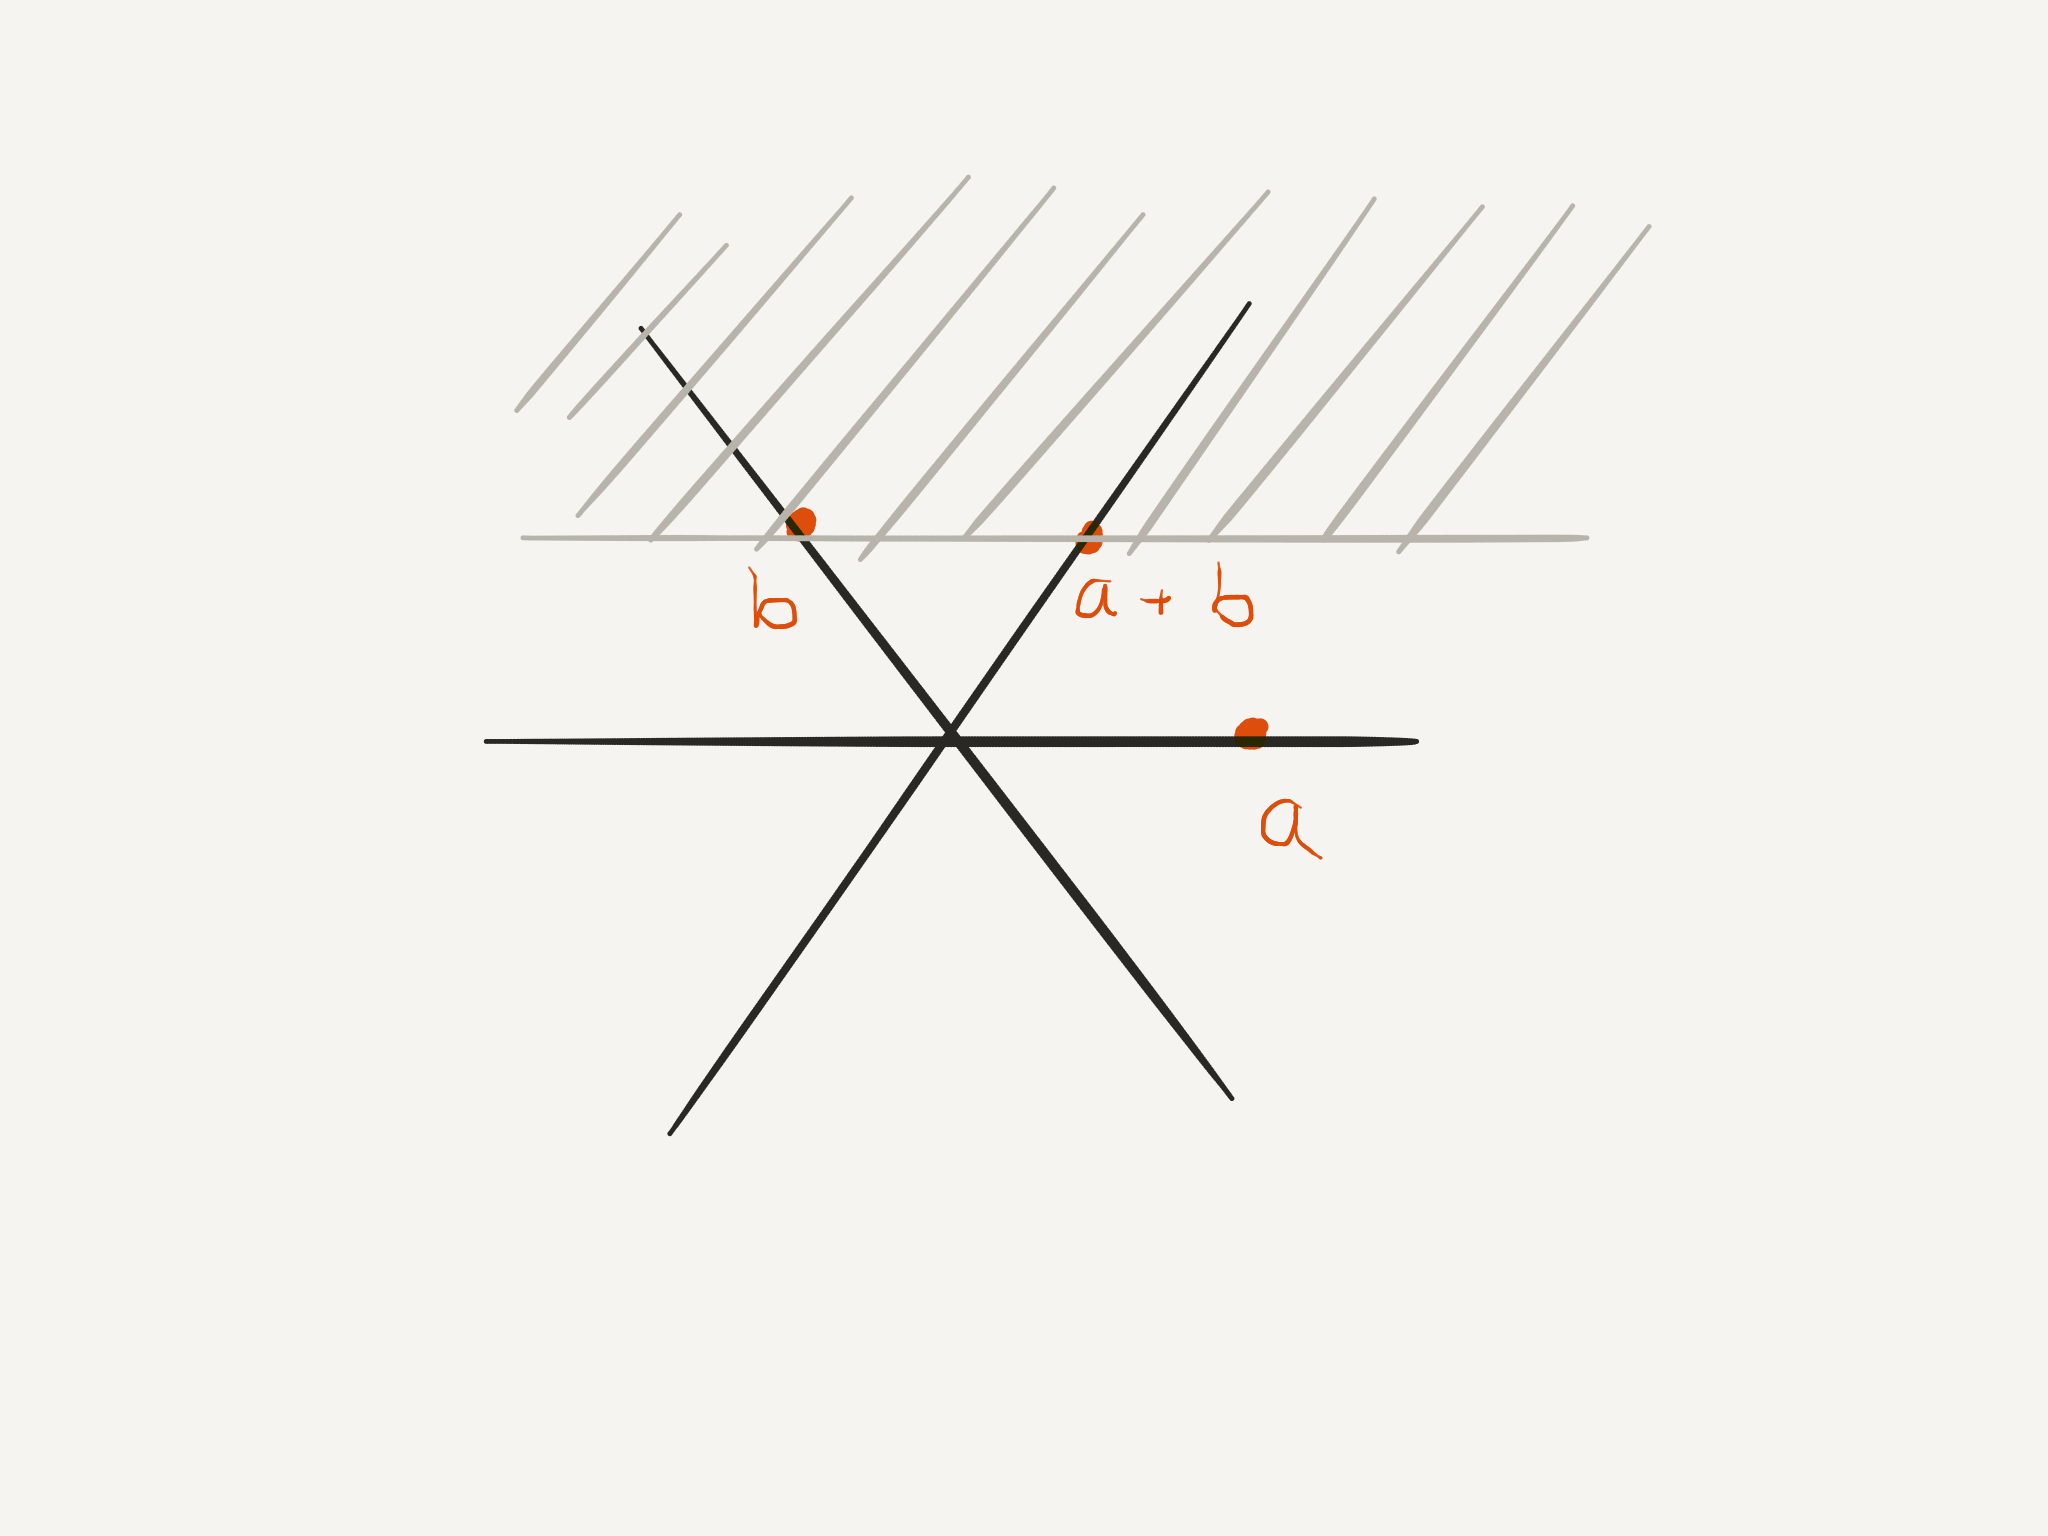
\includegraphics[scale=.25]{249-2.png}
\caption{The $A_2$ root system corresponding to $SL_3$. We can find a subsemigroup, such as 
an affine half-space, meeting the set of roots in $\{b, a+b\}$ but not in $\{a, b\}$.}
\end{figure}
\end{example}


\subsection{Subgroups corresponding to root semigroups}
Let $G$ be a connected linear algebraic group over a field $k$ equipped with an action by a $k$-torus $S$. (Reductivity will play \emph{no} role in this discussion.) 

For $H = S \ltimes G$, we have $Z_H(S) = S \times G^S$, where $G^S$ is the functorial centralizer of $S$, defined as the fixed points of the $S$-action. Passing to $H$ reduces many problems to the 
more familiar case of the conjugation action by a subtorus. 

\begin{example} For $S = \G_m $, we have $S \times G^S = Z_H(\lambda)$ for 
\begin{align*}
\lambda \colon \G_m = S &\hookrightarrow S \ltimes G \\
s & \mapsto (s,1)
\end{align*}
\end{example}


\noindent \textbf{Setup.} Let $\text{wt}_S(G) = \{ a \in {\rm{X}}(S) \mid \mf{g}_a \neq 0 \}$. 
We want to exponentiate (spans of) suitable $S$-weight spaces to $S$-stable
connected linear algebraic subgroups (with $S$-stability ensuring a uniqueness that cannot be guaranteed
by the Lie algebra alone in positive characteristic).

\begin{lemma}\label{lemwt} The set of
$S$-weights on the augmentation ideal $I_G \subset k[G]$ lie in the sub-semigroup 
$\langle \text{wt}_S(G) \rangle $ generated by $\text{wt}_S(G)$. 
\end{lemma}

\begin{proof} Since $G$ is connected, its coordinate ring $k[G]$ is a domain and hence injects into 
the local noetherian ring $k[G]_{I_G}$. This local ring is filtered by powers of its maximal ideal
and so each nonzero element of its maximal ideal has nonzero image in 
$I_G^n/I_G^{n+1}$ for some $n > 0$ by the Krull Intersection Theorem.  
Any successive quotient $I_G^n/I_G^{n+1}$ is a quotient of $(I_G/I_G^2)^{\otimes n}$, and 
$I_G/I_G^2 = \mf{g}^*$. This is all $S$-equivariant (giving $\mf{g}^*$ the linear dual action by $S$).
\end{proof}

\begin{remark}Depending on how you define the action of $G$ on its coordinate
ring, the weights which show up are those claimed or their negations (of course, this difference blurs in the case of the action of the commutative $S$, especially when the set of weights which occur on the Lie algebra
is stable under negation as for the conjugation on a connected reductive group by a split
maximal torus).
\end{remark}

\begin{proposition}\cite[Prop.\,3.3.6]{pred}\label{3.3.6}
Let $A \subset {\rm{X}}(S)$ be a subsemigroup $($i.e., a subset set,
possibly empty, stable under addition$)$. There is a unique $S$-stable connected linear algebraic $k$-subgroup $H_A(G) \subset G$ with the property that 
\[
\Lie(H_A(G)) = \bigoplus_{a \in A \cap \text{wt}_S(G)} \mf{g}_a.
\]
Moreover, $H_A(G)$ enjoys the following properties. 
\begin{enumerate}
\item $($maximality$)$ If $H \subset G$ is an $S$-stable connected linear algebraic 
$k$-subgroup such that $\text{wt}_S(\mf{h}) \subset A$ then $H \subset H_A(G)$. 
\item If $0 \notin A$ then $H_A(G)$ is unipotent $($denoted $U_A(G)$ for emphasis$)$. 
\end{enumerate}
\end{proposition}

\begin{remark}
The weight spaces $\mathfrak{g}_a$
for nonzero $a$ can be pretty large because of the generality: in particular, they are not necessarily lines! 
\end{remark}

\begin{proof}[Idea of proof] 
We're going to explain the idea of the proof if $0 \notin A$, as happens
in most cases of interest. (When $0 \in A$, one has
to include $G^S$ in the construction below.) 

To build $H_A(G)$, we want to construct things with $A \cap {\rm{wt}}_S(G)$ showing up in the Lie algebra. For each $a \in A \cap \text{wt}_S(G)$, consider the $k$-subgroup 
scheme $Z_G(\ker a) \subset G$, which is smooth 
even if $\ker a$ is non-reduced 
since $\ker a \subset S$ (see near the start of \S\ref{zisog}); this subgroup might be disconnected.

How does $S$ act on $Z_G(\ker a)$ ? Well, $\ker a$ acts trivially, so the $S$-action factors through the quotient 
$S/\ker a$, which can be identified \emph{via} $a$ with $\G_m$. Let 
\[
\lambda_a \colon \G_m \times Z_G(\ker a) \rightarrow Z_G(\ker a)
\]
be the induced action. Note that $\lambda_a$ is \emph{not} a one-parameter subgroup, but by the 
semi-direct product trick as discussed above we can apply all of the dynamic formalism
to $\G_m$-actions on affine group schemes of finite type. Hence, we can make sense of 
$U_{Z_G(\ker a)} (\lambda_a)$ as a unipotent smooth $k$-group
that is moreover connected (as groups $U_H(\mu)$ arising in the dynamic formalism are always
connected, even when $H$ is not, since the limiting definition provides an affine line from each geometric
point to the identity point.).

This construction extracts the part of the Lie algebra with weights which are \emph{positive} with respect to $\lambda_a$. That is, the Lie algebra of $U_{Z_G(\ker a)} (\lambda_a)$ 
consists of the \emph{positive} integral multiples of $a$ that are $S$-weights on $\mathfrak{g}$: 
\[
\Lie U_{Z_G(\ker a)} (\lambda_a) = \bigoplus_{b \in \text{wt}_S(G) \cap \Z_{\geq 1} a} \mf{g}_b.
\]

 Define the $S$-stable connected linear algebraic subgroup
\[
H_A(G) = \langle U_{Z_G(\ker a)} (\lambda_a) \rangle_{a \in A \cap \text{wt}_S(G)} \subset G.
\]
The real content is to show that its Lie algebra doesn't have unexpected weights. The key is that 
we control the weights showing up in the coordinate ring of each $U_{Z_G(\ker a)} (\lambda_a)$, and the group generated by these has a dominant multiplication map from a direct product of finitely many of these
groups (perhaps with high multiplicity); that realizes the coordinate ring of $H_A(G)$ as an $S$-equivariant
$k$-subalgebra of a tensor product of finitely many copies of the $U_{Z_G(\ker a)}(\lambda_a)$'s.
So the fact that this has the expected Lie algebra is ultimately due to Lemma \ref{lemwt}. 

How do we show unipotence of $H_A(G)$ when $0 \notin A$? Let $H := S \ltimes H_A(G)$. Then $Z_H(S)$ 
has Lie algebra $\mf{h}^S = \Lie(S)$ since $0 \notin A$, so the inclusion $S \subset Z_H(S)$ is equality. Hence $S$ is a \emph{maximal} $k$-torus in $H$, so in particular the dimension of the maximal tori of $H$
(i.e., its {\em rank}) is $\dim S$. This implies that $H_A(G)$ has trivial maximal torus - for instance, 
by working over $\ol{k}$ we see that 
$$\dim S = \rank H = \dim S + \rank H_A(G) ,$$
so $\rank H_A(G) = 0$, implying that $H_A(G)$ is unipotent. 

\end{proof}



\begin{example}\label{rootgpdef}
Let $G$ be a connected reductive group with \emph{split} maximal $k$-torus $T$. 
By Proposition \ref{3.3.6},
for $a \in \Phi(G, T)$ there is a unique connected linear algebraic group $U_a \subset G$ that is $T$-stable with $\Lie(U_a)$ having as its set
of $T$-weight $\text{wt}_T(G) \cap \langle a \rangle = \{ a\}$, where $\langle a \rangle$ denotes
the subsemigroup $\{ na \}_{n \geq 1}$. So we know that $U_a$ is unipotent with $\Lie(U_a) = \mf{g}_a$ a \emph{line}. Therefore, $\dim U_a = 1$. We call this the {\em $a$-root group}. 

We would like to show that $U_a \simeq \G_a$; this is a special case of
Proposition \ref{uagsplit} below. Once this is proved, 
since $\Aut_{k_s}(\G_a) = k_s^{\times}$ (true over \emph{fields} but not arbitrary bases!) it would follows that transporting
the $T$-action on $U_a$ over to $\G_a$ becomes 
$$t \cdot x = a(t) x$$
(as the action of each $t \in T(k_s)$ is scaling by some element of $k_s^{\times}$, and the actual
scalar can be read off from the action on the Lie algebra of $\G_a$). 

The unique characterization of $U_a$ implies that if $f:G \rightarrow G'$ is a central isogeny 
and for the split maximal $k$-torus $T' := f(T) \subset G'$ we denote by $a' \in \Phi(G',T')$ the root corresponding to $a$ as in Proposition
\ref{central_isog_roots} then $f$ carries $U_a$ {\em isomorphically} on $U_{a'}$ (so the formation of root groups
is insensitive to passing to central isogenous quotients!).  Indeed, if we choose generic $\lambda \in {\rm{X}}_{\ast}(T)$ (i.e., $\langle b, \lambda \rangle
\ne 0$ for all $b \in \Phi(G,T)$) then $\lambda' := f \circ \lambda$ is generic for $(G', T')$ and in the proof of Proposition \ref{central_isog_roots}
we saw that $f$ carries $U_G(\lambda)$ isomorphically onto $U_{G'}(\lambda')$.  Since necessarily $U_a \subset U_G(\lambda)$
and $U_{a'} \subset U_{G'}(\lambda')$, the unique characterization forces the isomorphism $f:U_G(\lambda) \simeq U_{G'}(\lambda')$
to carry $U_a$ isomorphically onto $U_{a'}$.  This reasoning applies {\em verbatim} when $G' = G/Z$ for any (not necessarily finite)
central closed $k$-subgroup scheme $Z \subset G$; i.e., the formation of root groups is compatible with central quotients.
\end{example}


\begin{example}[Rosenlicht]\label{rosenlicht} If $k$ is not perfect, then we can always make unipotent, connected, 1-dimensional $k$-groups which are \emph{not} $\G_a$! If $c \in k - k^p$ for $p = {\rm{char}}(k)$ then take 
\[
U = \{ y^p = x-cx^p\} \subset \A^2  = \G_a \times \G_a.
\]
Its closure in $\PS^2$ has one point, which is regular, at the line at $\infty$. However, this point is not rational (it is $\Spec k(\sqrt[p]{c})$). Therefore, $U $ is not isomorphic to $\A^1_k$, since the 
unique regular compactification of $\A^1_k$ has a unique point at $\infty$ that is moreover $k$-rational. 
\end{example}

In general, $U_A(G)$ is filtered by $\G_a$'s in the following sense:

\begin{definition}
Let $U$ be a unipotent connected linear algebraic $k$-group. We say that $U$ is \emph{$k$-split} 
if there exists a composition series $\{U_j\}$ of connected linear algebraic $k$-subgroups such that 
\[
U_j/U_{j+1} \simeq \G_a.
\]
We say that $U$ is \emph{$k$-wound} if it has no copy of $\G_a$ as a $k$-subgroup;
 i.e. if there is no $k$-subgroup inclusion $\G_a \hookrightarrow U$. 
\end{definition}

\begin{example}
Inside $\GL_n$, $\mathscr{R}_u(B)$ is split for a Borel subgroup $B$. 
On the other hand, Rosenlicht's construction in Example \ref{rosenlicht} is $k$-wound.
\end{example}

Tits' structure theory of unipotent groups is developed in a self-contained
modern manner in \cite[App.\,B]{pred} (also addressed in Appendix \ref{solvgp}), 
including split and wound connected unipotent linear algebraic 
groups and properties of these groups. \\

\noindent \textbf{Warnings.} The notions of {\em split} and {\em wound}
for connected unipotent linear algebraic $k$-groups are not as robust as in the theory of 
$k$-tori (i.e. where there is a notion maximal split $k$-torus the quotient by which is  $k$-anisotropic, and maximal $k$-anisotropic $k$-subtorus
the quotient by which is $k$-split).
\begin{enumerate}
\item Rosenlicht's wound group is a $k$-subgroup of a split $k$-group $\G_a \times \G_a$.
\item \cite[Ex.\,B.2.3]{pred} gives a $\G_a$-quotient of a wound $k$-group. 
\end{enumerate}

\begin{proposition}
If $k$ is perfect, then every unipotent connected linear algebraic $k$-group $U$ is $k$-split. 
\end{proposition}

\begin{proof}
See \cite[15.5(i)]{Borel} or \cite[B.2.5]{pred}. 
\end{proof}

Actually, we'll need a slightly more general result, as follows. For tori 
we noted above that there is a robust theory of split subtori with anisotropic quotient and vice-versa. For unipotent groups, we only have one of the two: a maximal split smooth connected $k$-subgroup 
$U_s$ such that $U/U_s$ is $k$-wound. More precisely, by 
\cite[B.3.4]{pred}, for any unipotent connected linear 
algebraic $k$-group $U$, there exists a unique $k$-split connected smooth 
$k$-subgroup $U_s \triangleleft U$ such that $$\ol{U} := U/U_s$$ is $k$-wound (and the formation of $U_s$ is compatible with separable extension of $k$). 

 \begin{remark}
 Whereas the formation of $U_s$ is compatible with separable extensions on $k$,
 the analogue for tori is only compatible with purely inseparanble extensions.
  \end{remark}


\begin{proposition}\label{uagsplit}
If $0 \notin A$, then $U_A(G)$ is $k$-split. 
\end{proposition}


\begin{proof}
For $U = U_A(G)$, we want to show that $\ol{U} = 1$. By design, if $\ol{U} \neq 1$ then $\text{wt}_S(\ol{U}) \subset \text{wt}_S(U) \subset A$ is non-empty. 
But it is a general fact \cite[B.4.4]{pred} that a wound group (such as $\ol{U}$)
can only admit a trivial action by a torus (such as $S$). 
\end{proof}

\begin{example}\label{weil_rest}
If $k'/k$ is a nontrivial finite separable extension, and $G' $ is a split connected reductive $k'$-group with $T' \simeq \G_m^r \subset G'$ the split maximal torus, consider  the Weil restriction
\[
G := {\rm{R}}_{k'/k} (G').
\]
We claim that this is connected reductive, with maximal $k$-torus $T := {\rm{R}}_{k'/k}(T')$ since this can be checked over $k_s$ (and we know that $G_{k_s} \simeq \prod_{\sigma : k' \hookrightarrow k_s} G' \otimes_{k, \sigma} k_s$,
and likewise for $T$). So a maximal torus for $G$ is $T = {\rm{R}}_{k'/k}(\G_m^r) \supset \G_m^r =: S$. 
(Later we will show that in a connected reductive group over a field,
all maximal split tori are rationally conjugate to each other; $S$ is such a $k$-torus for $G$.) 
As an exercise, check that via the identification ${\rm{X}}(S) = {\rm{X}}(T')$, we have 
\[
\Phi(G, S) = \Phi(G', T') 
\]
and $\mf{g}_b = \mf{g}_b'$ as $k$-vector spaces
(so of dimension $[k':k] > 1$), and at the level of roots groups $U_b = {\rm{R}}_{k'/k}(\G_a) \simeq \G_a^{[k':k]}$. 
\end{example}

\subsection{Direct spanning of root subgroups}

Let $(G,T)$ be a {\em split reductive pair} over $k$ (i.e. $G$ is a connected reductive $k$-group and $T$ a split maximal $k$-torus). Let $\Phi = \Phi(G,T) \subset {\rm{X}}(T) - \{0\}$ be the set of roots with respect to this pair.\\

\noindent \textbf{Some reminders.} Recall that we showed that the central isogeny 
\[
Z \times \Cal{D}(G) \rightarrow G,
\]
where $Z$ is the maximal central $k$-torus of $G$, induces isomorphisms
\[
{\rm{X}}(T)_{\Q} = {\rm{X}}(\Cal{T})_{\Q} \oplus {\rm{X}}(Z)_{\Q}.
\]
where $\Cal{T} := T \cap \Cal{D}(G)$ is a (split) maximal $k$-torus of $\Cal{D}(G)$, and 
\[
\Phi = \Phi(\Cal{D}(G), \Cal{T}) \times \{0\}.
\]
 Since $\Cal{D}(G)$ has trivial maximal central torus, we know that the inclusion
 $\Z \Phi \subset {\rm{X}}(\Cal{T})$ has finite index, so $\Q \Phi = {\rm{X}}(\Cal{T})_{\Q}$ inside ${\rm{X}}(T)_{\Q}$. 
 
For $c \in \Phi$, we have a root group $U_c \simeq \G_a$ inside $Z_G(T_c)$, and 
\[
 \Cal{D}(Z_G(T_c)) = \SL_2 \text{ or } \PGL_2
\]
since it is connected semisimple 
and split of rank 1:  the codimension-1 torus $T_c \subset T$ must be maximal central in $Z_G(T_c)$
(as $T$ isn't central) and we have the central isogeny 
\[
\Cal{D}(Z_G(T_c)) \times T_c \rightarrow Z_G(T_c)
\]
satisfying
\[
\Cal{T}_c \times T_c \twoheadrightarrow T
\]
where $\Cal{T}_c := T \cap \mathscr{D}(Z_G(T_c))$ is a 1-dimensional {\em split} torus.
The identification of $\mathscr{D}(Z_G(T_c))$ with ${\rm{SL}}_2$ or ${\rm{PGL}}_2$
can be chosen to carry $\Cal{T}_c$ over to the diagonal. 
This implies that the only non-trivial dependencies over $\Q$ among a pair roots are for $\pm c$,
and that $\langle U_c, U_{-c} \rangle = \mathscr{D}(Z_G(T_c))$. \\

As an application of the ubiquity of $\SL_2$ inside split connected semisimple groups, we 
obtain an important fact in characteristic 0 (never used in this course): 

\begin{proposition}\label{completered}
If $G$ is connected reductive over a field $k$ of characteristic $0$
then every linear representation of $G$ on a finite-dimensional $k$-vector space $V$ is completely
reducible.
\end{proposition}

In contrast, for any field $K$ whatsoever and any linear representation 
$V$ of smooth connected {\em unipotent} $K$-group $U$, the subspace $V^U$ is nonzero (as we may check
over $\overline{K}$ via the Lie--Kolchin theorem).

\begin{proof}
Let's check that we can assume $k=k_s$ (so tori become split).  
This will be mainly an application of the structure theory of finite-dimensional algebras
over fields \cite[XVII]{Lang}.  Suppose complete reducibility holds
for $V' := V_{k_s}$.  Let $A \subset {\rm{End}}_k(V)$ be the
Galois descent of $k_s[G(k_s)] \subset {\rm{End}}_{k_s}(V')$.
Assuming $V'$ is a semisimple $G_{k_s}$-representation,
so it is a semisimple $A_{k_s}$-module 
(as $G(k_s)$ is Zariski-dense in $G_{k_s}$ since $G$ is $k$-smooth), 
$A_{k_s}$ is a semisimple ring by \cite[XVII, Prop.\,4.7]{Lang}.
Thus, $A_{k_s}$ has no nonzero nilpotent 2-sided ideal, so 
the same holds for $A$.  Such vanishing 
characterizes semisimplicity for finite-dimensional algebras over fields
(see \cite[XVII, Thm.\,6.1]{Lang}), so $A$ is semisimple. 
The $A$-module $V$ therefore decomposes as a direct sum of simple
$A$-modules \cite[XVII, Prop.\,4.1]{Lang}.  But a $k$-subspace of $V$
is $G$-stable if and only if it is an $A$-submodule (as each can be checked over $k_s$), so $V$ is
completely reducible for $G$ as desired.

Now we may assume $k=k_s$.  
Let $Z \subset G$ be the maximal central torus and $G' = \mathscr{D}(G)$. 
Since $Z$ is split, $V$ decomposes into weight spaces for $Z$.
The groups $G'$ and $Z$ commute inside $G$, so the $G'$-action on $V$ preserves
each $Z$-weight space.
It suffices to treat these weight spaces as $G$-representations separately, 
so we are reduced to the case where $Z$ acts through a 
$\G_m$-valued character.  Now a subspace is stable under $G$ if and only if it is
stable under $G'$, so we may focus on $G'$; i.e., we may assume $G$ is semisimple. 
So far we haven't used that $k$ has characteristic 0!

The crucial fact is that $\mathfrak{g} := {\rm{Lie}}(G)$ is a semisimple Lie algebra.
In the theory of finite-dimensional Lie algebras in characteristic 0 as developed in
\cite[I, \S6]{bourbaki1}, semisimplicity is defined as the vanishing of commutative
Lie ideals and it is proved that the linear representation theory
of such Lie algebras is completely reducible.  Hence, it suffices
to prove two things:  $\mathfrak{g}$ has no nonzero commutative Lie ideal
(so it is semisimple) and that a subspace of $V$ is $G$-stable
if and only if it is $\mathfrak{g}$-stable  (under the Lie algebra representation
 $\mathfrak{g} \rightarrow {\rm{End}}(V)$).  The proofs of each will use
characteristic zero in a crucial way (and are false in every positive characteristic). 

Let $W \subset V$ be a subspace.  We claim that $W$ is $G$-stable if and only if it is
$\mathfrak{g}$-stable. 
The ``only if'' direction is obvious.  To prove the converse,  inside ${\rm{GL}}(V)$
consider the subgroup $H$ of linear automorphisms preserving $W$.  It is easy to check by computations
with a basis of $V$ extending one of $W$ that the Lie subalgebra $\mathfrak{h} \subset {\rm{gl}}(V)$
consists of the endomorphisms of $V$ preserving $W$.  The hypothesis
gives that for our representation $\rho:G \rightarrow {\rm{GL}}(V)$, ${\rm{Lie}}(\rho)$ lands
inside $\mathfrak{h}$, and we want to prove that the scheme-theoretic
preimage $\rho^{-1}(H)$ coincides with $G$.  By Cartier's theorem
(characteristic 0!) $\rho^{-1}(H)$ is smooth, so it suffices to show that it has
full Lie algebra inside $\mathfrak{g}$. 
The formation of tangent spaces is compatible with fiber products, 
so $\rho^{-1}(H)$ has Lie algebra
${\rm{Lie}}(\rho)^{-1}(\mathfrak{h}) = \mathfrak{g}$. 

Finally, we check that any commutative Lie ideal $\mathfrak{c}$
in $\mathfrak{g}$ vanishes. 
Since ${\rm{Lie}}({\rm{Ad}}_G) = {\rm{ad}}_{\mathfrak{g}}$,
any Lie ideal is stable under ${\rm{Ad}}_G$ by the equivalence of
$G$-stability and $\mathfrak{g}$-stability for subspaces of $G$-representations.
Thus, $\mathfrak{c}$ is a $G$-subrepresentation of $\mathfrak{g}$.  
Let $T \subset G$ be a maximal torus, so $\mathfrak{c}$ is a $T$-subspace
of $\mathfrak{g}$. If $\mathfrak{c}$ supports a nonzero $T$-weight
then it contains some root line $\mathfrak{g}_a$.  But the subgroup
$\langle U_a, U_{-a} \rangle \subset G$ that is $\SL_2$ or ${\rm{PGL}}_2$ 
contains the standard Weyl element that swaps $a$ and $-a$, so by $G$-stability
$\mathfrak{c}$ would also contain $\mathfrak{g}_{-a}$.
The common Lie algebra $\mathfrak{sl}_2$ of $\SL_2$ and $\PGL_2$ away from characteristic 2 
is generated as a Lie algebra by its opposite root lines, so $\mathfrak{c}$
would have to contain $\mathfrak{sl}_2$, contradicting that $\mathfrak{c}$ is commutative.

Hence, the $T$-action on $\mathfrak{c}$ is trivial, which is to say
$\mathfrak{c} \subset \mathfrak{g}^T = {\rm{Lie}}(Z_G(T)) = {\rm{Lie}}(T)$. But
$T$ was {\em arbitrary}!
By noetherian induction, the intersection $\bigcap_T T$ of all maximal tori
coincides with the intersection $T_1 \cap \dots \cap T_n$
of finitely many. This intersection coincides with the center $Z_G$ by Corollary \ref{ztori}, so 
$$\mathfrak{c} \subset \cap_j {\rm{Lie}}(T_j) = {\rm{Lie}}(\cap_j T_j) = {\rm{Lie}}(Z_G).$$
But $Z_G$ is finite since $G$ is semisimple, and it is {\em smooth} (Cartier's theorem, once again),
so ${\rm{Lie}}(Z_G) = 0$. 
\end{proof}

Now we consider linearly independent roots $c,c' \in \Phi$ (i.e. $c' \neq \pm c$). Note that
\begin{align*}
A := & \langle c \rangle + \langle c' \rangle = \N c + \N c  \\
= &\{ ic + jc' \in \Phi \mid i,j \geq 1 \} =: (c,c')
\end{align*}
does \emph{not} contain $0$. Thus, by Proposition \ref{3.3.6} we have a unipotent connected
linear algebraic group 
\[
U_A(G) = \langle U_a \rangle_{a \in A \cap \Phi}.
\]
(The inclusion $\supset $ follows from maximality of $U_A(G)$, and $\subset$ because we know the Lie algebras coincide by our description of roots for a split reductive group, and the fact that an inclusion of smooth connected groups with the same Lie algebras is an isomorphism.) In fact we can do much better: we will show
that such groups $U_a$ ``directly span'' $U_A(G)$ under multiplication in any desired (but fixed) enumeration
of $A \cap \Phi$.  Before we discuss such a property, we record a general result on commutators.

\emph{Notation.} For smooth closed $k$-subgroups $H$ and $H'$ of a linear algebraic group $G$
over $k$, we denote by $(H,H')$ the subgroup generated by commutators of $H$ by $H'$. In the past this has usually been denoted $[H,H']$. 

\begin{proposition}\cite[Prop.\,3.3.5]{pred}\label{prop335}
 Let $G$ be a connected linear algebraic $k$-group with action by a split 
$k$-torus $S$.
\begin{enumerate}
\item If $H, H' \subset G$ are $S$-stable connected linear algebraic $k$-subgroups then 
\[
\text{wt}_S( (H, H')) \subset \text{wt}_S(H) + \text{wt}_S(H').
\] 
\item If $A,A' \subset {\rm{X}}(S)$ are subsemigroups, then
\[
(H_A(G) , H_{A'}(G)) \subset H_{A+A'}(G).
\]
\end{enumerate}
\end{proposition}

\begin{proof}[Remarks on proof]
Clearly (1) implies (2), by the maximality of $H_{A+A'}$ with respect to containing weights within $A+A'$. For (1), 
we get intuition from characteristic 0, since in such cases 
\[
\Lie((H,H')) = [\mf{h}, \mf{h}']
\]
and we have functoriality of the Lie bracket, so 
\[
t . [X,X'] = [t.X, t.X'] \text{ for } t \in S
\]
via the induced $S$-action on $\mathfrak{g}$.  A characteristic-free
proof is given in \cite{pred} by studying the $S$-action on coordinate rings. 
\end{proof}

\begin{example}
Let $(G,T)$ be a split reductive pair. For $c \in \Phi$, \emph{choose} a $k$-isomorphism 
\[
u_c \colon \G_a \simeq U_c. 
\]
By Proposition \ref{prop335}(2) we have 
\[
(U_c, U_{c'}) \subset U_{\langle c \rangle + \langle c' \rangle}(G) =  \langle U_a \rangle_{a \in (c,c')}.
\]
The right side is ``directly spanned'' by  $\{U_a\}_{a \in (c,c')}$ (where $(c,c'):= (\langle c \rangle + \langle c' \rangle) \cap \Phi$) in the sense of the following definition.
\end{example}

\begin{definition}
A linear algebraic $k$-group $H$ is \emph{directly spanned} by smooth closed $k$-subgroups $H_1, \ldots, H_n \subset H$ if for \emph{any} permutation $\sigma$ of $\{1, \ldots, n \}$ the multiplication map 
\[
H_{\sigma(1)} \times \ldots \times H_{\sigma(n)} \rightarrow H 
\]
is an isomorphism of $k$-schemes. 
\end{definition}

The direct-spanning result to be recorded shortly
has nothing to do with reductive groups (not even in the proofs), being instead about the action of a split
$k$-torus $S$ on any connected linear algebraic $k$-group $G$.
Let $A \subset {\rm{X}}(S)$ be a subsemigroup not containing $0$. Consider a decomposition
\[
A \cap \text{wt}_S(G) = \coprod \Psi_i
\]
where $\Psi_i$ is disjoint from the subsemigroup $A_j := \langle \Psi_j \rangle$ for all $j \neq i$; i.e. the subset $A \cap {\rm{wt}}_S(G)$ breaks up into pieces which do not intersect even when some mild addition is permitted.

\begin{example}
Here is a prototypical example for the setup: let $(G,S)$ be a split reductive pair and 
\[
A = \{ \chi \in {\rm{X}}(S) \colon \langle \chi, \lambda \rangle > 0 \} \text{ for a regular } \lambda \in {\rm{X}}_*(S).
\]
We may take $\Psi_i = \{a_i\}$ for $\{a_1, \ldots, a_n\} =  \Phi_{\lambda > 0} = \Phi_{\lambda \geq 0}$.
 \end{example}

%consider $\mathscr{R}_u(B)$ for a split reductive pair $(H,S)$ and a Borel $k$-subgroup $B \supset S$. The roots are all in one half-plane, so they are pairwise linearly independent.) 


\begin{theorem}\cite[Thm.\,3.3.11]{pred}\label{3311}
The $k$-group $U_A(G)$ is directly spanned by $\{U_{A_j}(G) \}$. 
\end{theorem}

\begin{proof}[Idea of proof] 
Note that each $U_{A_i}(G) = U_{A_i}(U_A(G))$ because $U_{A_i} \subset U_A(G)$ a priori from the maximality property. Hence, we can replace $G$ with $U_A(G)$ so that $G$ is \emph{unipotent}. Now this is one of the rare instances where want to use the descending central series (remember that unipotent is nilpotent, so the descending central series terminates). This is a good thing to do because the difficulty with these direct spanning results is the rampant non-commutativity. 

If $G$ is non-commutative then we have via the {\em canonical}
descending central series an $S$-equivariant exact sequence 
\[
1 \rightarrow Z \rightarrow G \rightarrow G/Z \rightarrow 1
\]
with $Z \subset G$ a nontrivial smooth connected central $k$-subgroup. We perform dimension induction
via such centrality to reduce to the case of \emph{commutative} $G$.  

In characteristic 0,
a commutative unipotent group is a vector group.
In characteristic $p>0$ we use the composition series $\{p^i G\}$ to reduce to the case when
$G$ is also $p$-torsion.  Now the key is to use the structure theory in \cite[App.\,B]{pred}
for unipotent connected linear algebraic groups equipped with 
a sufficiently nontrivial action by a split torus (via the hypothesis $0 \not\in A$)
to ensure that such a commutative $G$ also killed by $p$ in characteristic $p$
is necessarily a {\em vector group} (i.e., $\G_a^n$)
on which the $S$-action is {\em linear} relative to {\em some} linear structure
(beware that $\G_a^2$ admits many non-linear automorphisms in characteristic $p > 0$,
such as $(x, y) \mapsto (x + y^p, y)$). The complete reducibility of linear
representations of a split torus then yields the desired result. 
\end{proof}

\begin{example}
If $(G,T)$ is a split reductive pair then 
\[
\{ \text{Borels} \supset T \}  = \{ P_G(\lambda) \supset T \text{ for regular } \lambda \in {\rm{X}}_*(T)\}.
\]
Thus, for any such $B$ we have $\mathscr{R}_{u,k}(B) = U_G(\lambda)$ using such a regular
$\lambda$, so $\mathscr{R}_{u,k}(B) = U_{c_1} \times \ldots \times U_{c_n}$ via
multiplication for any enumeration $\{c_1, \ldots, c_n\}$ of $\Phi_{\lambda > 0} = \Phi(B, T)$.

Note in particular (as can also be proved directly from the dynamic description) that a Borel 
$k$-subgroup containing $T$ is determined by the set of roots $\Phi(B, T)$
(as $B = T \ltimes \mathscr{R}_{u,k}(B)$). A consequence of this is that there is a unique {\em opposite Borel} $B' \subset G$ containing $T$ and satisfying $B' \cap B = T$; this characterization of $B'$ in terms of $B$ and $T$
makes sense without requiting $T$ to be split, and in that generality its existence and uniqueness
can be deduced immediately from the split case over $k_s$ via Galois descent.
\end{example}


\begin{proposition}\label{commutation}
Consider a split reductive pair $(G,T)$ and $c,c' \in \Phi := \Phi(G,T)$ with $c' \neq \pm c$. Fix a parametrization $u_{c''} \colon \G_a \simeq U_{c''}$ for all $c'' \in \Phi$. Then 
\[
(u_c(x), u_{c'}(x)) = \prod_{a  = i c+ jc'\in (c,c')} u_a(m_{i,j,c,c'} x^i y^j)
\]
for some $m_{i,j,c,c'} \in k$ using a fixed enumeration of $(c,c')$. 

$($The structure constants $m_{i,j,c,c'}$ depend on the enumeration and parametrizations $\{u_a\}$$)$. 
\end{proposition}

Before we prove this result, we make some remarks.
Chevalley showed that for suitable parameterizations one can always arrange the 
structure constants to arise from 
specific \emph{integers} determined up to sign solely by the enumeration and (root system) $\Phi$. 
It turns out that such integers lie in  $\{\pm 1, \pm 2, \pm 3\}$;
see \cite[Prop.\,6.3.5, Rem.\,6.3.5]{luminy} and references therein.

\begin{example}\label{sp4ex}
Let $G= \Sp_4$ (root system $\Phi$ of type $B_2=C_2$) with the symplectic form 
\[
\psi(v,v') = v^T \begin{pmatrix} 0 & 1 \\ -1 & 0 \end{pmatrix} v'
\]
and maximal torus 
\[
T = \begin{pmatrix} t_1 \\ & t_2 \\ & & t_1^{-1} \\ & & & t_2^{-1} \end{pmatrix}.
\]

\begin{figure}
\centering
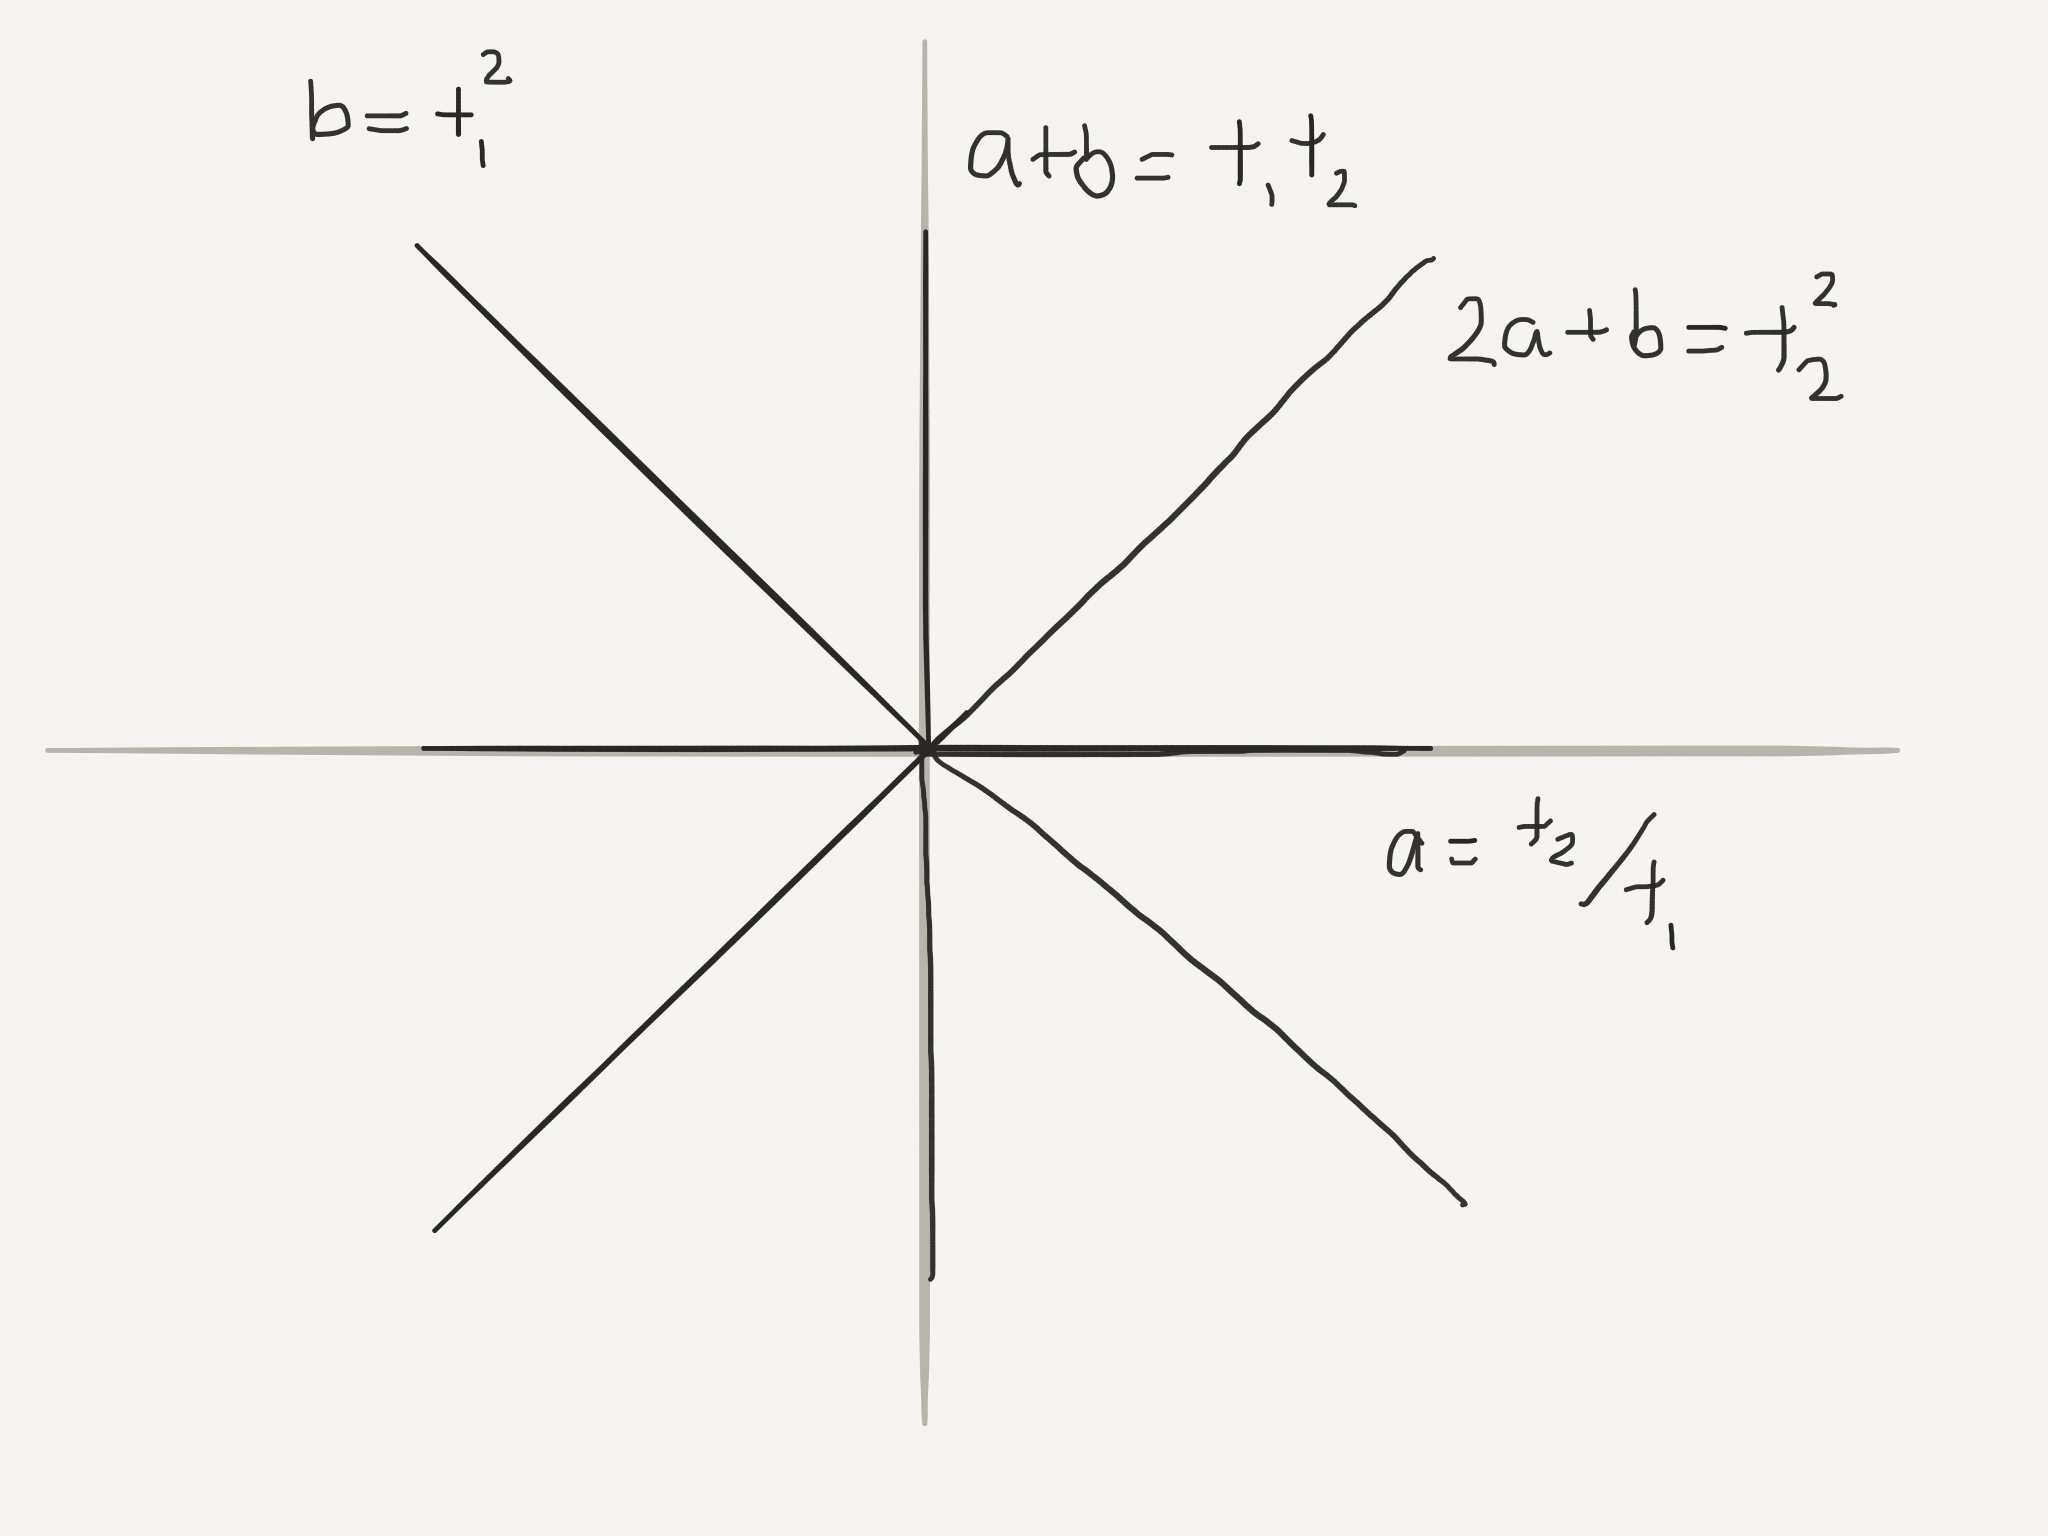
\includegraphics[scale=.25]{249-3.png}
\caption{Positive roots for the $B_2=C_2$ root system corresponding to $\Sp_4$.}
\end{figure}

We have parameterizations of corresponding root groups:
\begin{align*}
u_a(x) &= \begin{pmatrix} 1 &  \\ -x & 1 \\ & & 1 & x \\ & &  & 1 \end{pmatrix} \\
u_b(x) &= \begin{pmatrix} 1 & & x \\ & 1  \\ & & 1 & \\ & & & 1 \end{pmatrix} \\
u_{a+b}(x) &= \begin{pmatrix} 1 & & & x  \\ & 1 & x &  \\ & & 1 & \\ & & & 1 \end{pmatrix} \\
u_{2a+b}(x) &= \begin{pmatrix} 1  \\ & 1 & & x \\ & & 1 \\ & & & 1 \end{pmatrix}.
\end{align*}
The nontrivial commutation relations are
\begin{align*}
(u_a(x), u_b(y) )&= u_{2a+b}(x^2y) u_{a+b}(-xy), \\
(u_a(x), u_{a+b}(y)) &= u_{2a+b}(-2xy);
\end{align*}
$U_b$ and $U_{a+b}$ commute, as do $U_a$ and $U_{2a+b}$
(either by inspection or more conceptually because
the sets of roots $(b, a+b)$ and $(a, 2a+b)$ are empty!).
Note in particular that in characteristic 2 the second commutation
relation degenerates, or more specifically the root groups for $a$ and $a+b$ {\em commute}
in characteristic 2. 

\end{example}


\begin{proof}[Proof of Proposition \ref{commutation}]
We are considering a split reductive pair $(G,T)$ over $k$. Let $c,c' \in \Phi(G, T)$ be two roots with 
$c' \neq \pm c$. 
In Proposition \ref{prop335} we noted that there is a containment $[U_c, U_{c'}] \subset U_A(G)$ for $A = 
\langle c \rangle + \langle c' \rangle$ for formal reasons. (Note that $(c, c') = A \cap \Phi$.) 
Fix $k$-isomorphisms $u_b:\G_a \simeq U_b$ for all roots $b$.  Upon {\em fixing an enumeration}
of the set $(c,c')$ of roots $a = ic + jc'$ with $i, j \ge 1$, we have 
\[
[u_c(x), u_{c'}(y)] = \prod_{a \in (c,c') } u_a(F_a(x,y))
\]
for some $F_a: \mathbf{A}^2_k = U_c \times U_{c'} \rightarrow U_a = \mathbf{A}^1_k$;
i.e., $F_a \in k[x, y]$ (depending on the choice of enumeration
and on the parameterizations $u_b$ for roots $b$). 
Our task is to show that $F_a$ is a monomial, and more specifically of bi-degree $(i, j)$ where
$a = ic + jc'$.

The proof is a simple consequence of behavior under
conjugation against $T$.  There is no harm in assuming that $k = \ol{k}$. For any $t \in T(k)$, we have 
\begin{align*}
t[u_c(x), u_{c'}(y)] t^{-1} &= [tu_c(x) t^{-1} , tu_{c'}(y) t^{-1}] \\
&= [u_c(c(t)x), u_{c'}(c'(t)y)]\\
& = \prod_a u_a(F_a(c(t)x, c'(t)y)).
\end{align*}
On the other hand, 
\begin{align*}
t  \cdot \prod_{a \in (c,c') } u_a(F_a(x,y)) \cdot t^{-1} & = \prod_{a = ic+jc'} (tu_a(F_a(x,y))t^{-1}) \\
&= \prod_a u_a(a(t) F_a(x,y)).
\end{align*}

Therefore we must have a termwise equality:
\[
F_a(c(t)x, c'(t)y) = a(t) F_a(x,y) = c(t)^i c'(t)^j F_a(x,y)
\]
where $a = ic + jc'$. 
Now we are saved by the condition that the characters are linearly independent. We have a surjective map
\[
T \xrightarrow{(c,c')} \G_m \times \G_m.
\]
Therefore
\[
F_a(ux, vy) = u^i v^j F_a(x,y)
\]
for all  $x,y \in k$ and $u,v \in k^{\times}$.
By considering the contribution to both sides
from each monomial term appearing in $F_a$, this implies that $F_a(x,y) = f_{ij} x^i y^j$ for $f_{ij} \in k$.
\end{proof}

An important fact due to Chevalley, which we mentioned last time, is that there is a 
systematic choice of enumeration of $(c, c')$
and parameterizations $\{u_b\}$ which leads to $f_{ij} \in \{\pm 1, \pm 2, \pm 3\}$ determined solely
by $\Phi$. 

\begin{example}
Consider the split connected semisimple $k$-group $G = G_2$; this is the automorphism scheme of the
unique (up to isomorphism) split
octonion algebra over $k$ (see \cite[App.\,B]{zgroup}).
In this case, a split maximal $k$-torus $T \subset G$ has rank 2 and 
 $\Phi := \Phi(G, T)$ is a root system
of type G$_2$. Let $\{c, c'\}$ be a basis for this root system with $c$ short and $c'$ long as shown in the accompanying Figure. 

\[
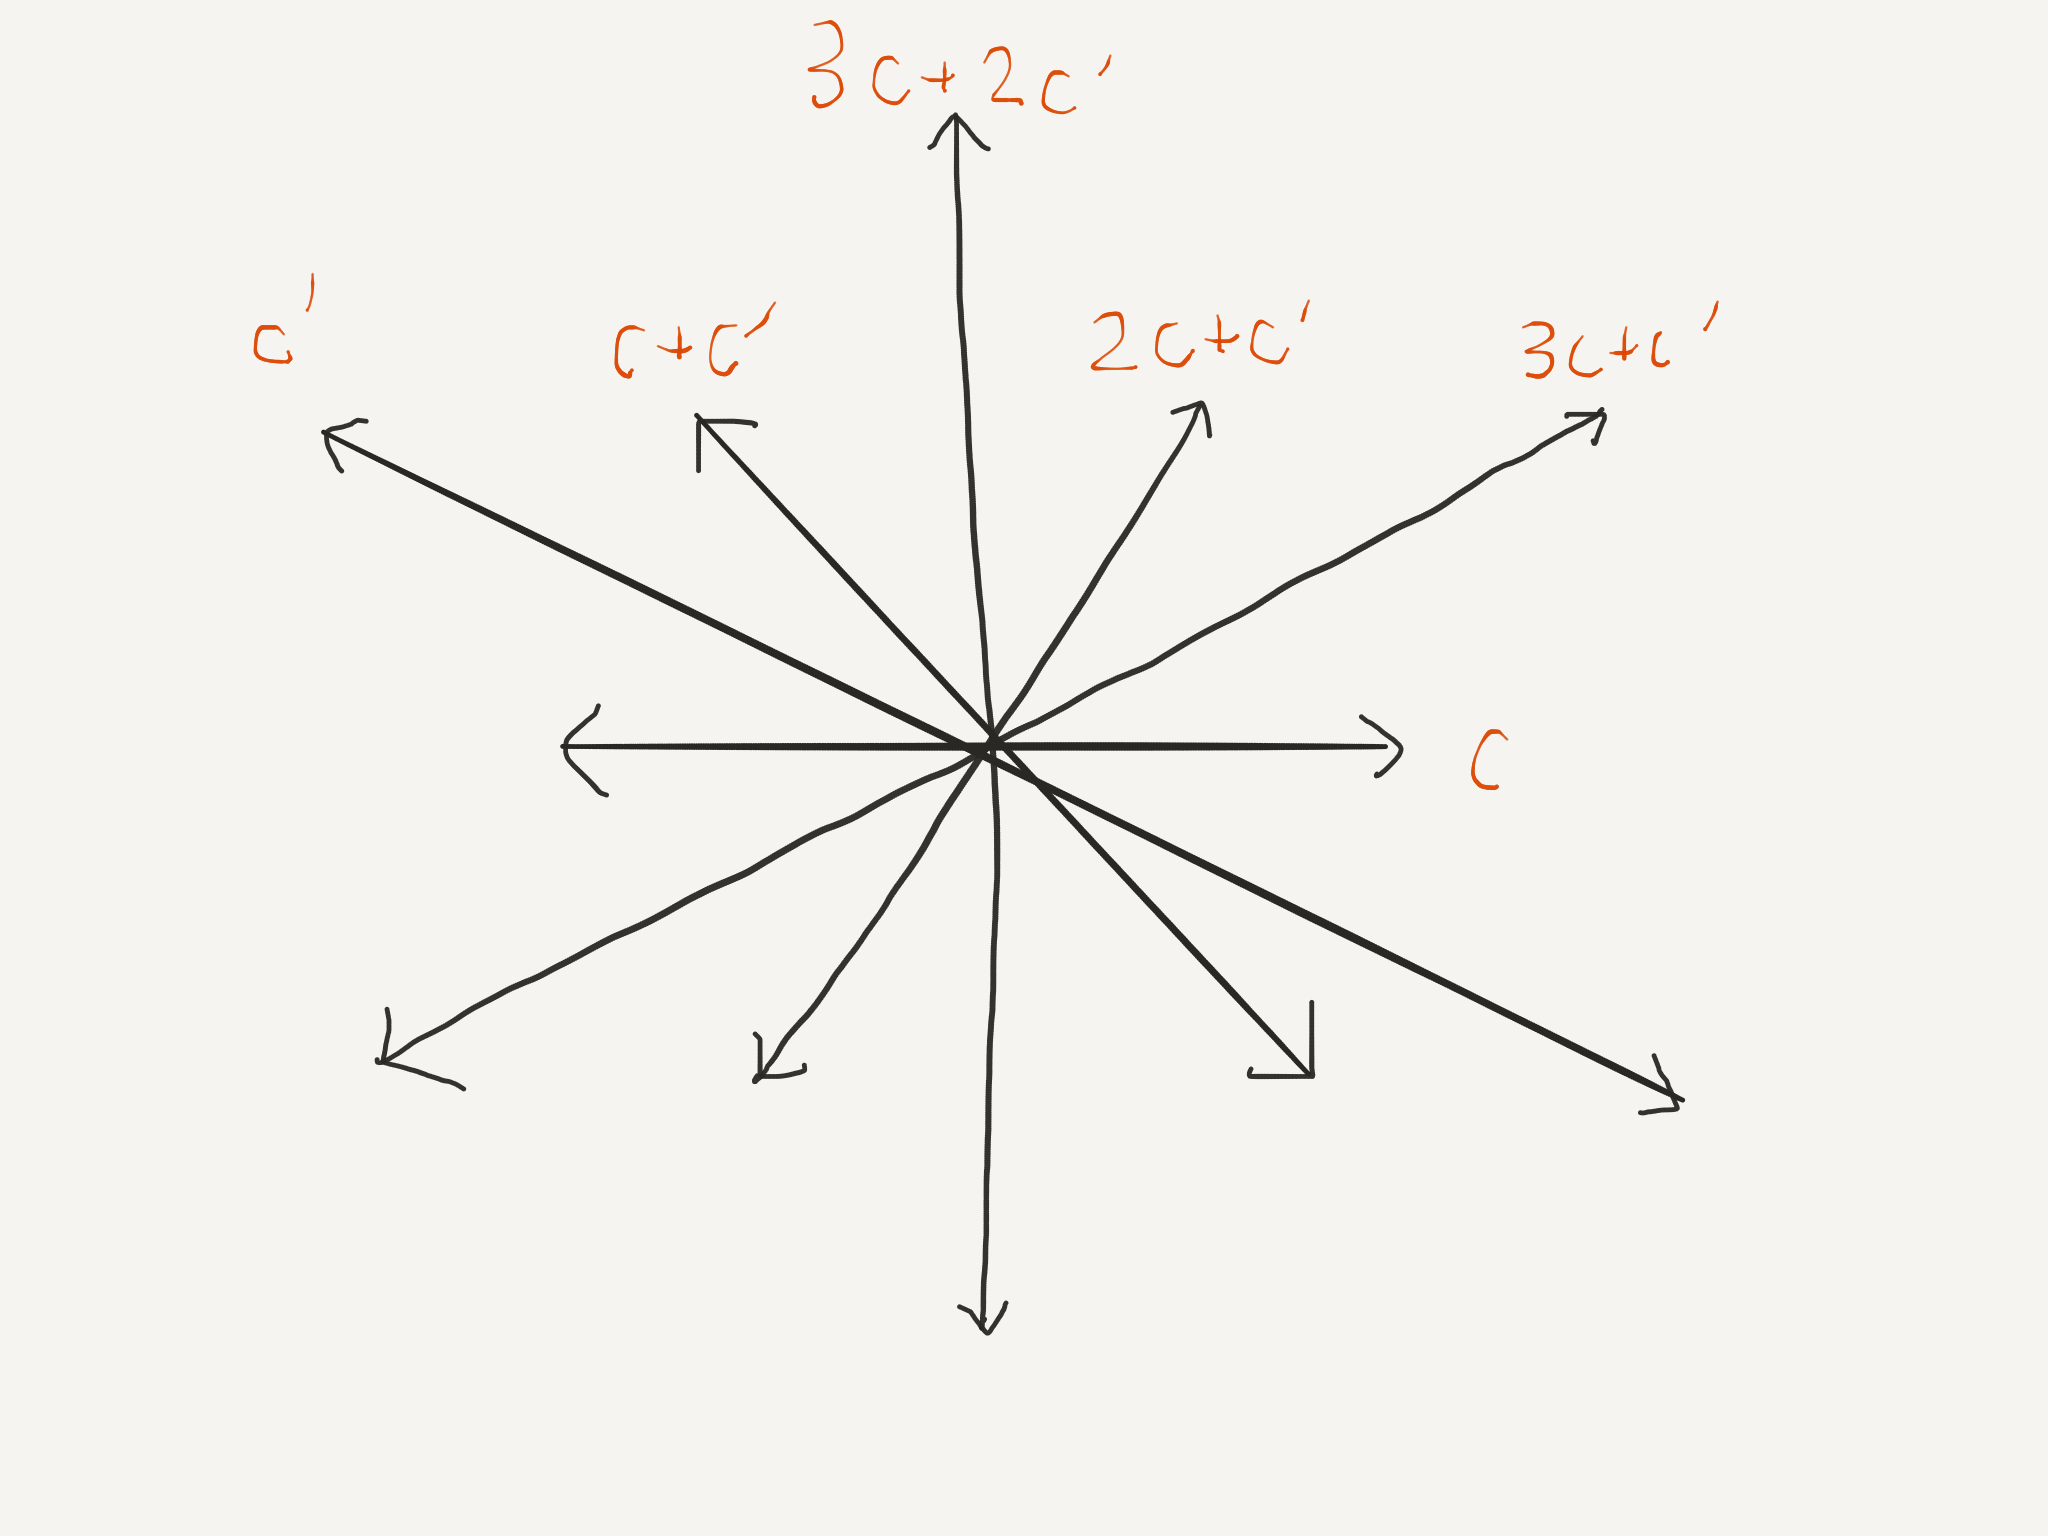
\includegraphics[scale=.25]{249-4.png}
\]


The set $(c,c')$ consists of $c+c', 3c+2c', 2c+c', 3c+c'$. It turns out that $f_{ij} = \pm 3$ does occur for this root system, using an appropriate enumeration of $(c, c')$ (see
\cite[Lemma 6.2.8, Ex.\,6.2.9]{luminy} and references therein 
or \cite[\S33.5]{humphreys} for the general form of Chevalley's commutation relations for G$_2$).
We now explain the consequence this has for the structure of $G$, especially in characteristic 3;
this will not be used in anything that follows.

From the picture and Chevalley's commutation relations, 
the span of the root lines 
for $c', c+c', 2c+c', 3c+c'$ is a 4-dimensional representation for the $k$-subgroup 
$\SL_2 \simeq G_c \rightarrow G = G_2$ generated by 
the root groups for $\{ \pm c\}$. 
\[
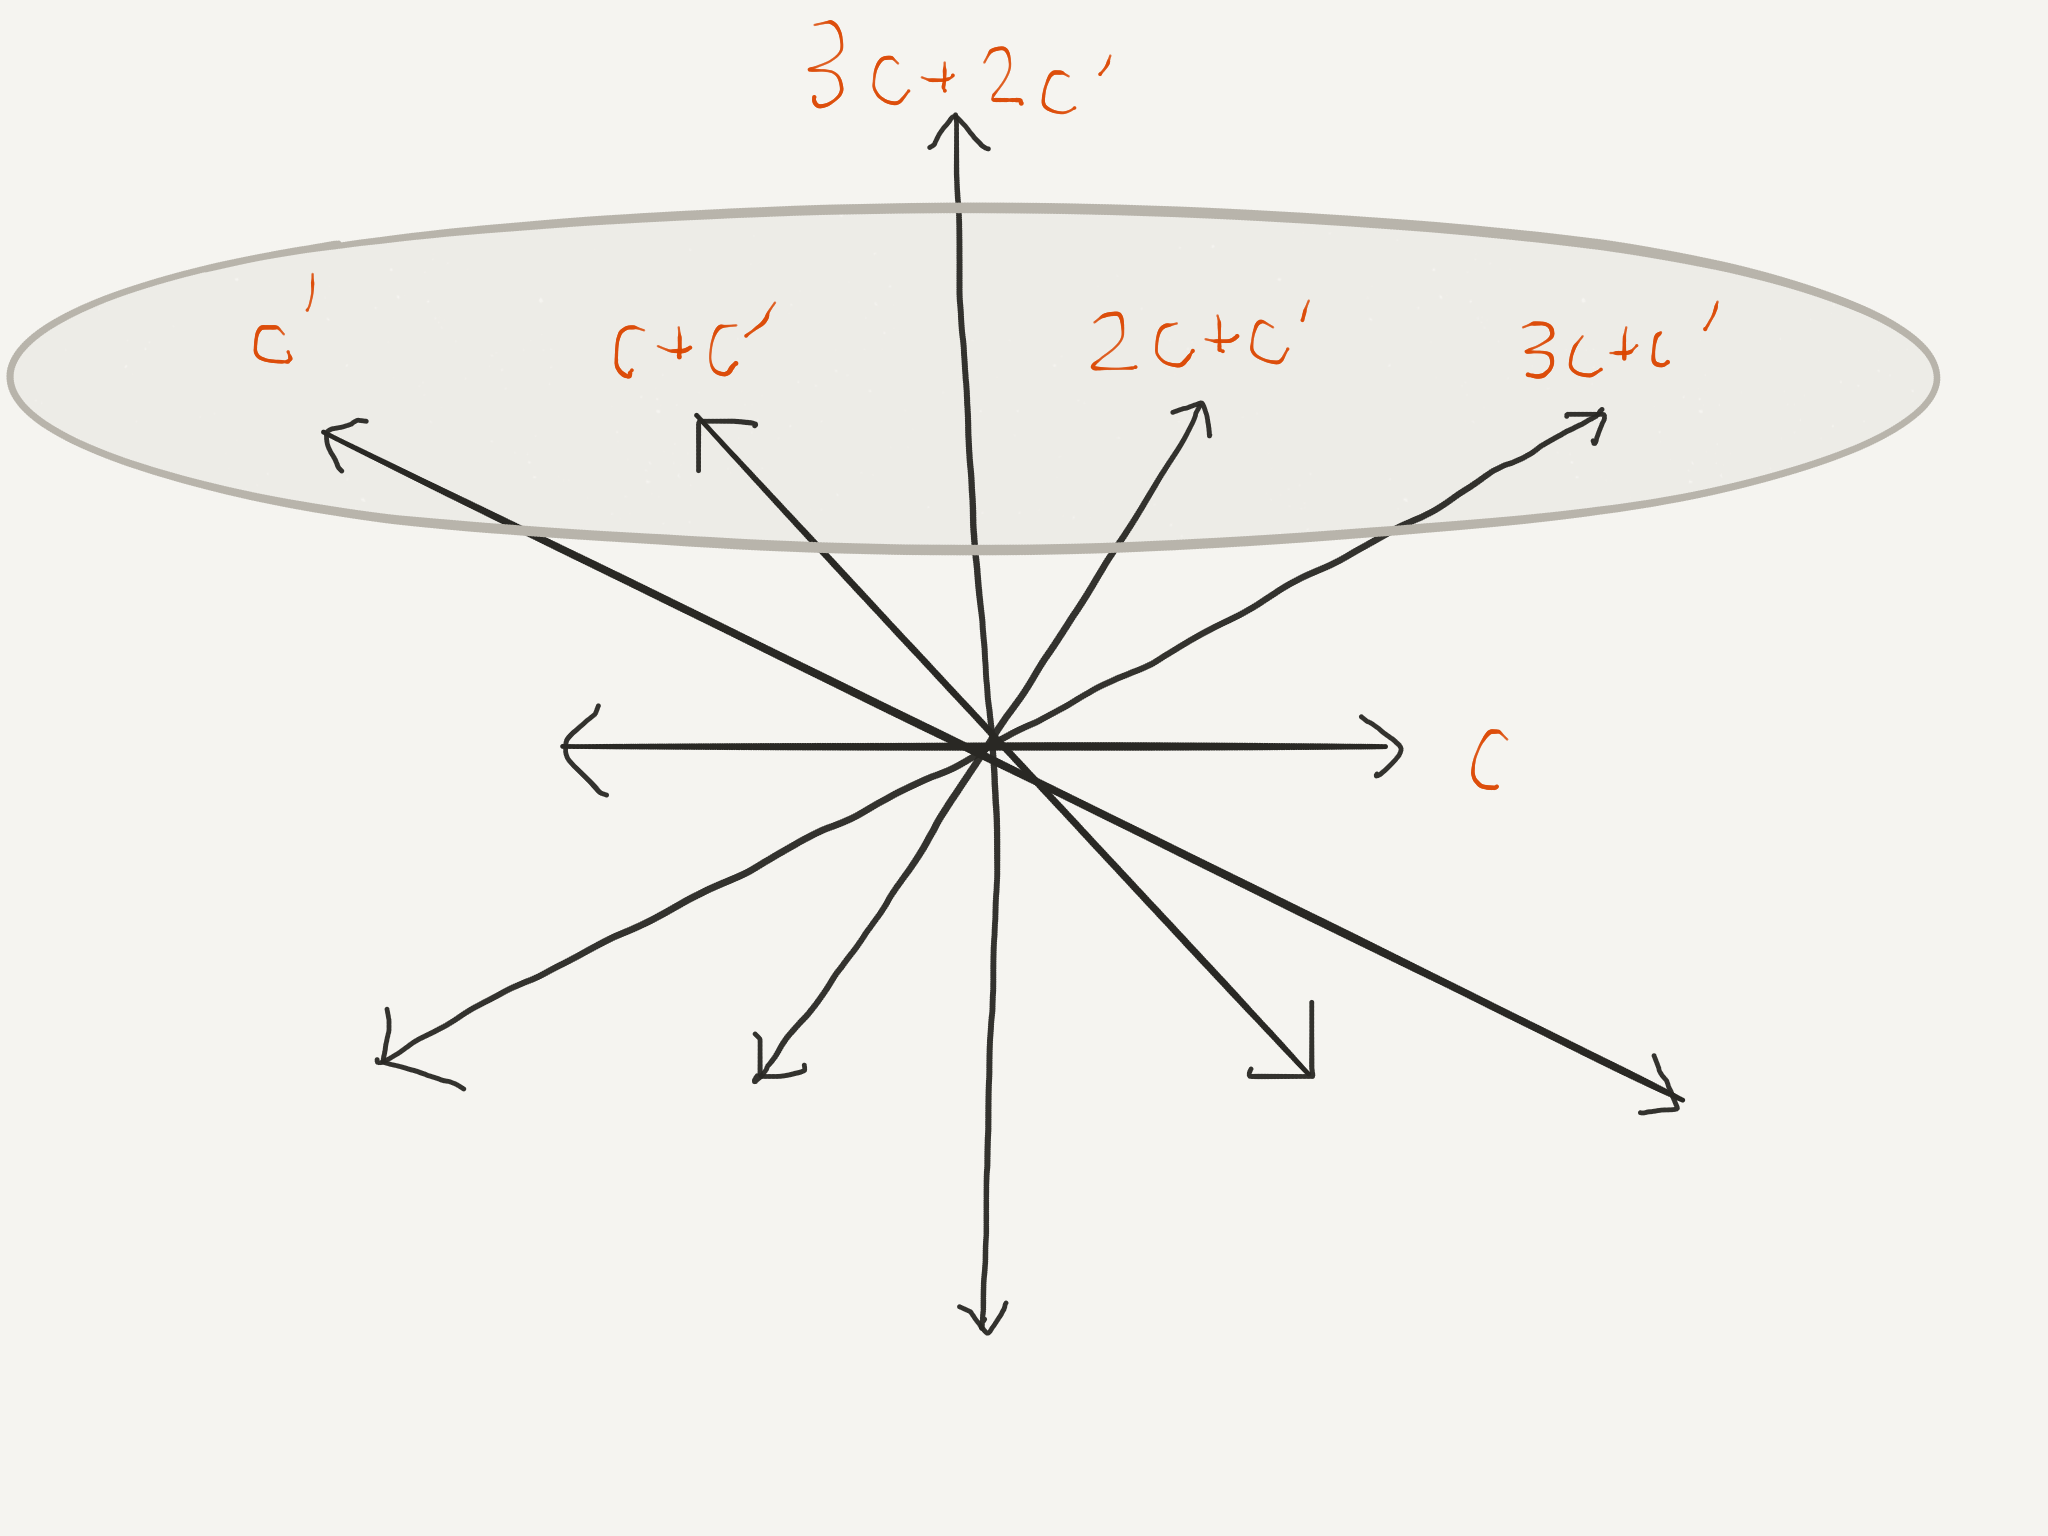
\includegraphics[scale=.20]{249-5.png}
\]

The corresponding four root groups together with the root group for $3c+2c'$  directly span
a unipotent group $U$ normalized by $G_c$; explicitly, $U = U_A(G)$ for an evident subsemigroup $A$
not containing 0. The form of the commutation relations
implies that the root group $U_{3c+2c'}$ corresponding to the highest root is the center
of $U$ and  that $\overline{U} := U/U_{3c+2c'}$ is abelian,
so there is a short exact sequence 
\[
1 \rightarrow Z_U = U_{3c+2c'} \rightarrow U \rightarrow \ol{U}  \rightarrow 1
\]
for which $\overline{U}$ is a vector group of dimension $4$ identified with the direct
product of the other 4 root groups.  That direct product structure on $\overline{U}$ yields
a linear structure on this vector group that is the {\em unique}
one equivariant with respect to the $T$-action; in this way we identify $\overline{U}$
with its Lie algebra $\mathfrak{h} = {\rm{Lie}}(\overline{U})$. 

The commutator of the root lines for $c+c'$ and $2c+c'$ is nonzero
and valued in the root line for $3c+2c'$, and similarly for the longer roots $c'$ and $3c+c'$ (by a computation in the root system for $\mf{sl}_3$). Hence, $U$ is a Heisenberg group:  there is a symplectic pairing on 
the quotient $\mathfrak{h}$ of $U$  valued in the $k$-subgroup $U_{3c+2c'} \subset U$.

We have built $\SL_2 = G_c$ acting on the 4-dimensional space $\mathfrak{h}$, and this action is linear (as we can check
using the actions of $U_c$ and $U_{-c}$). When ${\rm{char}}(k) \ne 2, 3$, we can conclude that $\mathfrak{h}$ is the unique 4-dimensional irreducible representation of $\SL_2$, so $\mathfrak{h} \simeq \Sym^3(V)$
where $V$ is the standard 2-dimensional representation of $\SL_2$. Letting
$\{e, e'\}$ denote the standard ordered basis for $V$, a basis for $\mathfrak{h}$
is $\{ e^3, e^2e', e{e'}^2, {e'}^3 \}$ relative
to which the ``raising operator''  $(\begin{smallmatrix} 1 & 1 \\ 0 & 1 \end{smallmatrix}) \in
\SL_2$ acts by $e \mapsto e$ and $e' \mapsto e+e'$. When we apply this
operator to ${e'}^3$, for instance, the coefficient $3$ shows up against $e{e'}^2$. 

Assume ${\rm{char}}(k)=3$. The irreducible 4-dimensional ${\rm{SL}}_2$-representations 
are $(V^{\otimes 3})^{S_3}$ and $(V^{\otimes 3})_{S_3}$. 
Inside $(V^{\otimes 3})^{S_3}$ is a copy of $V$ spanned by the symmetrizers of $e^{\otimes 2} \otimes e'$
and $e \otimes {e'}^{\otimes 2}$, the quotient by which is the Frobenius twist $V^{(3)}$ (using
$e^{\otimes 3} \mapsto e^{(3)}$ and ${e'}^{\otimes 3} \mapsto {e'}^{(3)}$).  Likewise,
$(V^{\otimes 3})_{S_3}$ contains a copy of $V^{(3)}$ spanned by the classes of
$e^{\otimes 3}$ and ${e'}^{\otimes 3}$, the quotient by which is $V$ (spanned by
images of the classes of $e^{\otimes 2} \otimes e'$ and $e \otimes {e'}^{\otimes 2}$).
This gives non-trivial extensions of ${\rm{SL}}_2$-representations:
\begin{align*}
0 \rightarrow V \rightarrow (V^{\otimes 3})^{S_3} \rightarrow V^{(3)} \rightarrow 0 \\
0 \rightarrow V^{(3)} \rightarrow (V^{\otimes 3})_{S_3} \rightarrow V \rightarrow 0
\end{align*}
These are distinguished by the unique 2-dimensional subrepresentations with weights
for the diagonal torus given by
$\pm 1$ for $(V^{\otimes 3})^{S_3}$ and $\pm 3$ for $(V^{\otimes 3})_{S_3}$ respectively.
\[
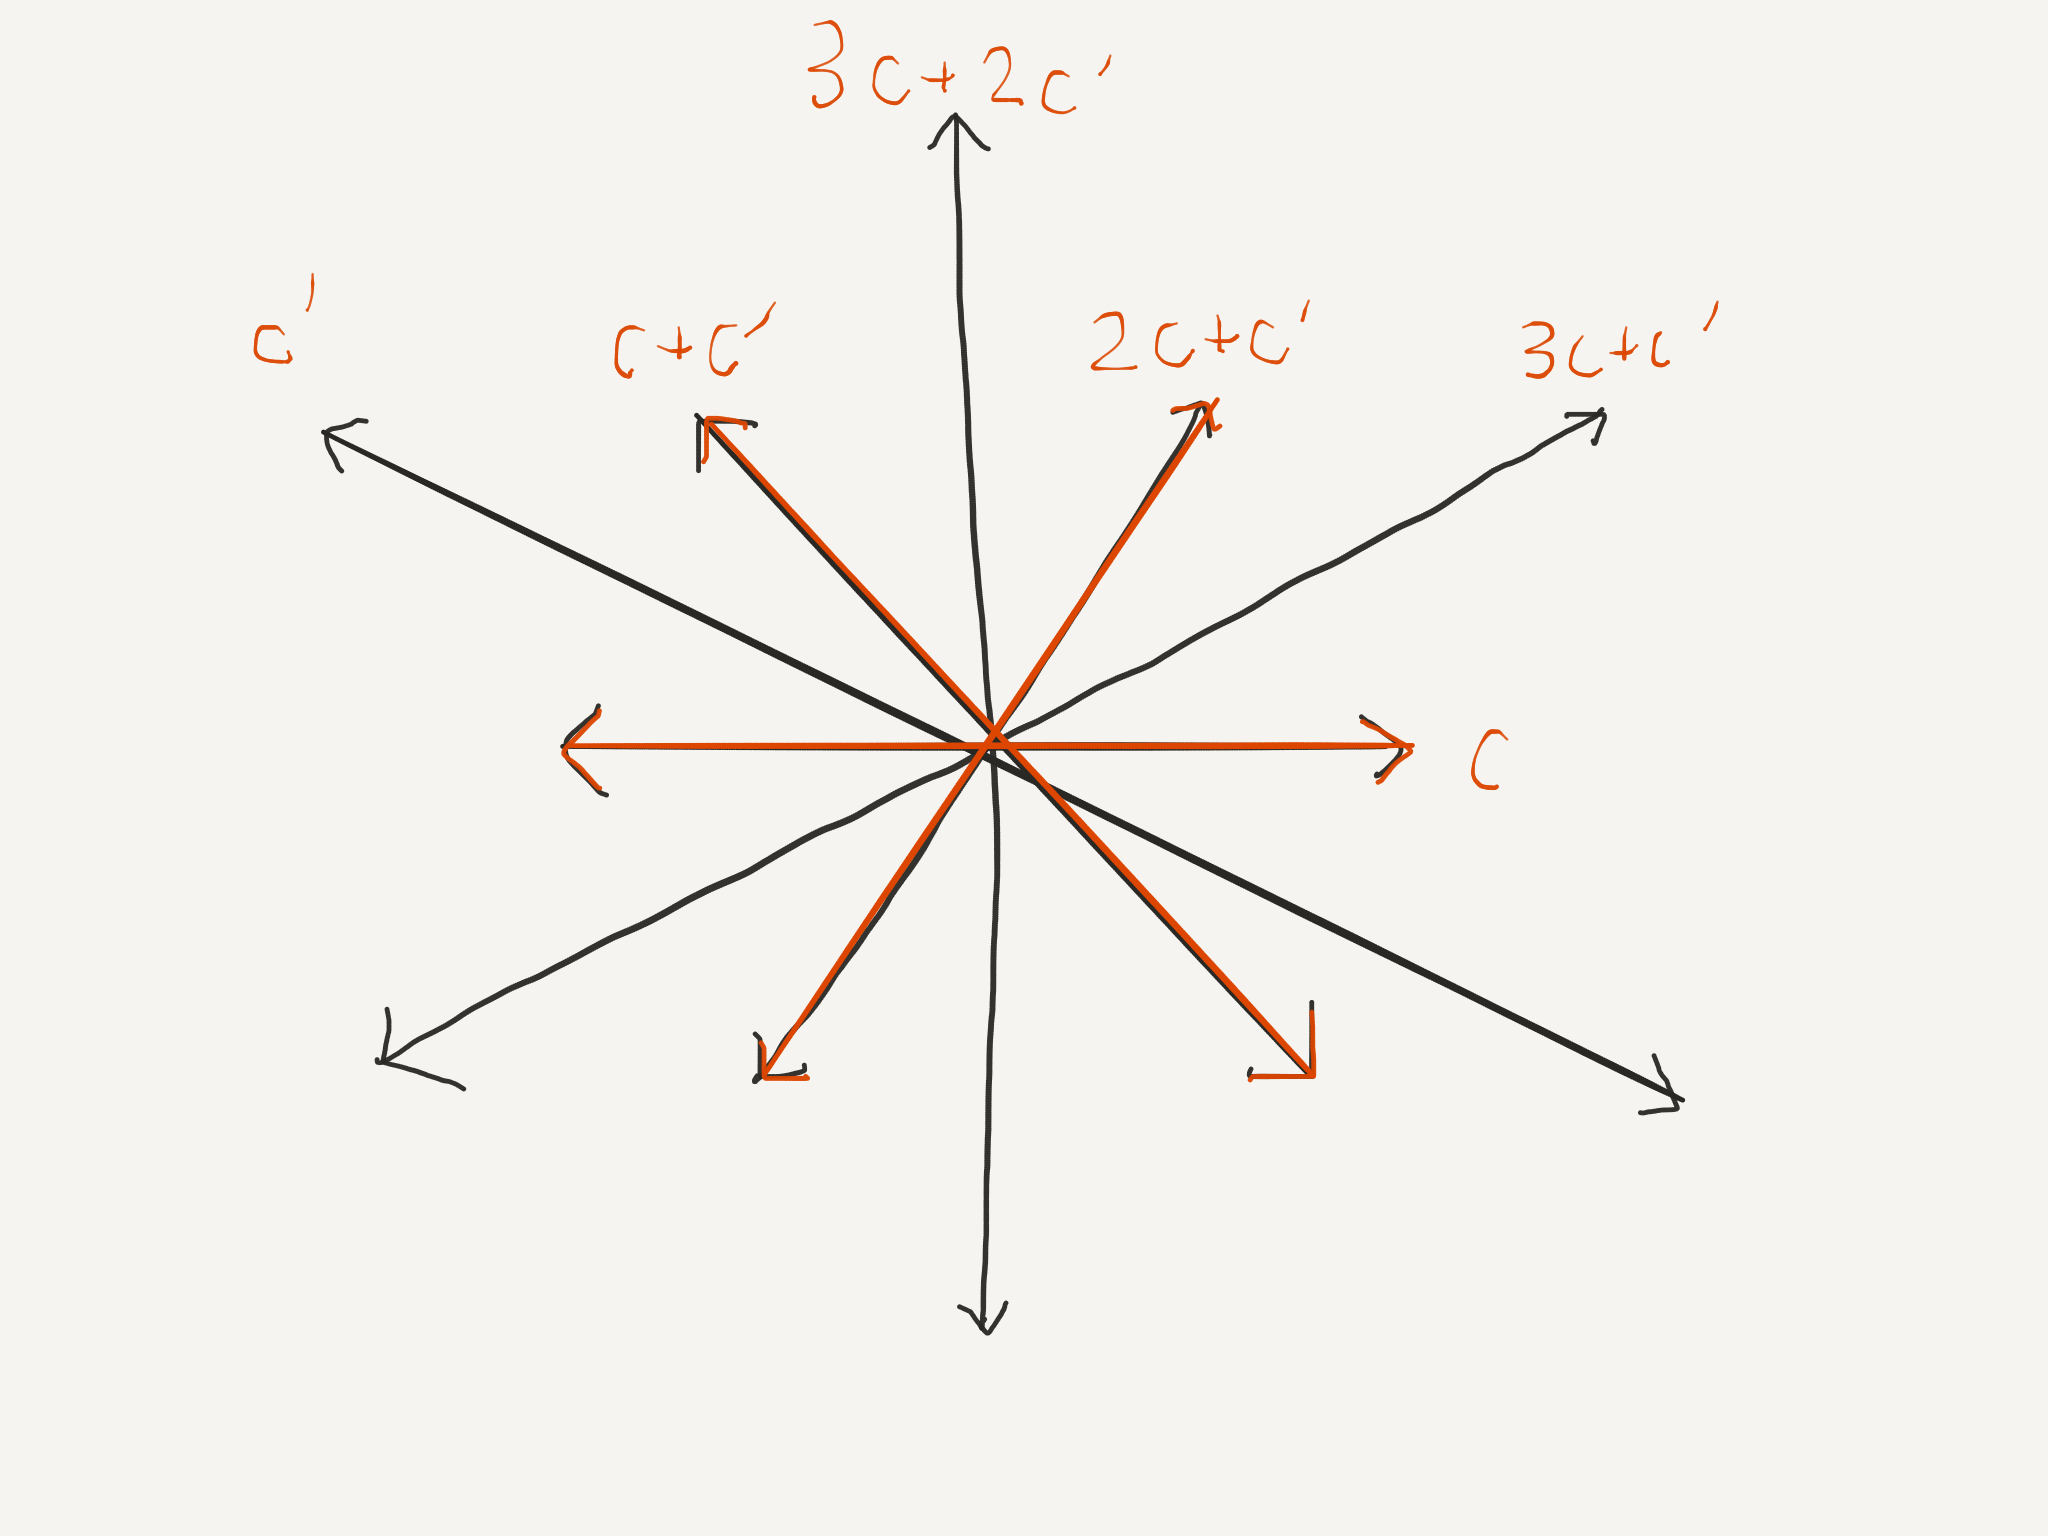
\includegraphics[scale=.2]{249-6.png}
\]

Is $\mathfrak{h}$ isomorphic to $ (V^{\otimes 3})^{S_3} $ or $(V^{\otimes 3})_{S_3}$? 
To answer this we shall calculate use some notions to be discussed
later, namely coroots (see \S\ref{corootsec}) and their encoding in terms of 
the Dynkin diagram or geometry of the root system. This gives
$\langle c, {c'}^{\vee} \rangle = -1$ and $\langle c', c^{\vee} \rangle = -3$, 
so the weights of the (split) maximal torus $c^{\vee}(\mathbf{G}_m) \subset G_c = {\rm{SL}}_2$
on the short root lines $\mathfrak{g}_{c+c'}$ and $\mathfrak{g}_{2c+c'}$ inside $\mathfrak{h}$ are $\mp 1$
and the weights of $c^{\vee}(\mathbf{G}_m)$ 
on the long root lines $\mathfrak{g}_{c'}$ and $\mathfrak{g}_{3c+c'}$ inside 
$\mathfrak{h}$ are $\mp 3$.
Thus, $\mathfrak{h} \simeq (V^{\otimes 3})^{S_3}$ precisely when the short root lines in $\mathfrak{h}$
span a $G_c$-stable subspace
(and then the span of the long root lines in $\mathfrak{h}$ is not $G_c$-stable).
We shall prove that the span of the short root lines is indeed $G_c$-stable.

The group $G_c = {\rm{SL}}_2$ is generated by the torus
$c^{\vee}(\mathbf{G}_m)$, the root group $U_c$,
and any representative for the nontrivial element of
$W(G_c, c^{\vee}(\mathbf{G}_m))$.  The adjoint action of $c^{\vee}(\mathbf{G}_m)$ preserves all root lines,
and the effect of a Weyl element swaps root lines according to the reflection $r_c$,
so this swaps the two short root lines inside $\mathfrak{h}$ as well as swaps the two
long root lines inside $\mathfrak{h}$.  Hence, everything comes down to determining
whether the adjoint action of $U_c$ preserves the span of the short root lines
inside $\mathfrak{h}$ or preserves the span of the long root lines inside $\mathfrak{h}$.
We shall prove that the former holds.

For suitable parameterizations of the root groups
the commutation relations for $U_c$ against $U_{c+c'}$  and $U_{2c+c'}$
degenerate in characteristic 3 to
\begin{align*}
u_{c+c'}(y)u_c(x) &= u_c(x) u_{c+c'}(y) u_{2c+c}(-2xy) \\
u_{2c+c'}(y) u_c(x) &= u_c(x)u_{2c+c'}(y).
\end{align*}
Thus, the adjoint action of $U_c$ on 
$\mathfrak{g}_{2c+c'}$ is trivial 
and on $\mathfrak{g}_{c+c'}$ is valued in $\mathfrak{g}_{c+c'} + \mathfrak{g}_{2c+c'}$,
so the span of the short root lines inside $\mathfrak{h}$ is $G_c$-stable as claimed.
That is, $\mathfrak{h} \simeq (V^{\otimes 3})^{S_3}$ as a representation for
$G_c = {\rm{SL}}_2$.

Note that the long roots constitute a root system of type A$_2$, and likewise for the short roots.
Hence, it is natural to ask if 
the long root groups are the root groups for a copy of ${\rm{SL}}_3$ or ${\rm{PGL}}_3$
(the two split connected semisimple groups with root system A$_2$) inside
G$_2$ containing $T$, and likewise for the short root groups.
In all characteristics (and even over $\Z$ with appropriate definitions) the long root groups
generate an SL$_3$ containing $T$ with those long roots as its $T$-root groups,
whereas precisely in characteristic 3 the short root groups 
are the root groups for a connected semisimple group of type A$_2$ containing $T$, and 
this special subgroup in characteristic 3 is PGL$_3$.  In \cite[\S7.1]{pred} 
this phenomenon is explained from a broader point of view.
\end{example}


\section{Dynamic description of parabolic subgroups}

\subsection{Main result}

We want to prove the following characterization of parabolic subgroups. 
It is difficult to overestimate the importance of this result.


\begin{theorem}\label{pardyn}
Let $G$ be a connected, reductive group (not necessarily split) over any field $k$. 
\begin{enumerate}
\item For every $k$-homomorphism $\lambda: \G_m \rightarrow G$ the $k$-subgroup $P_G(\lambda)$
is parabolic, and every parabolic $k$-subgroup of $G$ arises in this manner.
\item If $P$ is a parabolic $k$-subgroup of $G$ and $T \subset P$ is any maximal $k$-torus, then there exists 
a $k$-homomorphism $\lambda \colon \G_m \rightarrow T$ such that $P_G(\lambda)=P$. 
\end{enumerate}
\end{theorem}

\begin{remark}\label{partorus}
The generality is quite non-trivial. For instance, if $P \neq G$ then $\lambda$ is obviously nontrivial, so this implies that any maximal torus $T \subset P$ must have a non-trivial one-parameter $k$-subgroup. Thus, a consequence of this Theorem is that any maximal $k$-torus $T$ in a proper
parabolic $k$-subgroup of $G$ cannot be $k$-anisotropic.   

Since proper parabolic
$k$-subgroups of $G$ correspond bijectively to those of $\mathscr{D}(G)$, and the center of
$\mathscr{D}(G)$ is finite with the multiplication map $Z \times \mathscr{D}(G) \rightarrow G$ (where $Z$ is the maximal
central $k$-torus of $G$) being an isogeny, it follows from this Theorem that $G$ has a {\em proper}
parabolic $k$-subgroup if and only if $\mathscr{D}(G)$ contains a nontrivial split $k$-torus
(i.e., $\mathscr{D}(G)$ is $k$-isotropic, or equivalently $G$ contains a {\em non-central}
split $k$-torus). 

Indeed, by finiteness of the center of
$\mathscr{D}(G)$ it follows that if there is a nontrivial split
$k$-torus  $S$ in $\mathscr{D}(G)$ and 
$\lambda \in {\rm{X}}_{\ast}(S) - \{0\}$ then the {\em parabolic} $k$-subgroup $P_G(\lambda)$
must be proper (as otherwise $U_G(\lambda) = \mathscr{R}_{u,k}(G) = 1$, forcing
$G = P_G(\lambda) = Z_G(\lambda)$, contradicting that the nontrivial $\lambda:\G_m \rightarrow
\mathscr{D}(G)$ cannot be central in $Z \cdot \mathscr{D}(G) = G$). 
\end{remark}

We have already seen in Corollary \ref{borpar}  that for a maximal $k$-torus
$T \subset G$ the Borel 
subgroups of $G_{\overline{k}}$ containing
$T_{\overline{k}}$ are $P_G(\lambda)$ for regular $\lambda \colon \G_m \rightarrow T_{\overline{k}}$. 
This will be used in the proof of Theorem \ref{pardyn}.

To begin the proof of this Theorem, 
we first prove $P_G(\lambda)$ is a parabolic $k$-subgroup of $G$ for
any $k$-homomorphism $\lambda:\G_m \rightarrow G$. 
For this, we may assume that $k = \ol{k}$. We need to exhibit a Borel subgroup in $P_G(\lambda)$. 
Let $T \subset P_G(\lambda)$ be a maximal torus (so $T$ is also maximal in $G$). 
We'll produce a regular $\mu \colon \G_m \rightarrow T$ such that $P_G(\mu) \subset P_G(\lambda)$. Since $P_G(\mu)$ is a Borel subgroup of $G$, the parabolicity of $P_G(\lambda)$ would follows.

Visualizing the finite subset $\Phi \subset {\rm{X}}(T)_{\Q} - \{0\}$,
it is clear what to do: choose $\mu$ to be a small perturbation of $\lambda$. More precisely, we have
\[
\Phi(P_G(\lambda), T) = \{a \in \Phi \mid \langle a, \lambda \rangle  \geq 0\}.
\]
We can decompose this into two subsets $\Phi_{\lambda>0}$ and $\Phi_{\lambda = 0}$. Choose $\mu_0 \in {\rm{X}}_*(T)_{\Q}$ such that for each of the finitely many $a \in \Phi_{\lambda >0}$, we have $\langle a, \mu_0 \rangle > 0$. (Any $\mu_0$ close enough to $\lambda$ works.) Then take $\mu = N \mu_0$ for
a positive integer $N$ sufficiently divisible so that  $\mu \in {\rm{X}}_*(T)$, and 
$\mu$ will still have the same property. Let $B = P_G(\mu)$, a Borel subgroup.  

The crucial step is to show that $B$ is contained in $P_G(\lambda)$.  The set
\[
\Phi(B, T) = \{a \in \Phi \mid \langle a, \mu \rangle \geq  0 \}
\]
is a subset of 
\[
\Phi(P_G(\lambda), T) = \{a \in \Phi \mid \langle a, \lambda \rangle \geq  0 \}
\]
because the choice of $\mu$ forces 
$$\langle a, \lambda \rangle < 0 \implies \langle -a, \lambda \rangle > 0 \implies
\langle -a, \mu \rangle > 0 \implies \langle a, \mu \rangle < 0.$$ 
Hence, for the two smooth connected $k$-subgroups
$B, P_G(\lambda) \subset G$ containing $T$ we have
$${\rm{Lie}}(B) \subset {\rm{Lie}}(P_G(\lambda))$$
since each Lie algebra is the direct sum of ${\rm{Lie}}(T)$ and the root lines for
the respective roots for $T$ that occur in these Lie algebras. 
This does the job in characteristic $0$, but we need to do more work to give
an argument applicable in all characteristics:


\begin{lemma}\label{liecompare}
For $\lambda, \mu \in {\rm{X}}_*(T)$, if $\Phi(P_G(\mu), T) \subset \Phi(P_G(\lambda), T)$ then $P_G(\mu) \subset P_G(\lambda)$. 
\end{lemma}

\begin{proof}
We use the functoriality of the dynamical construction. Let $P = P_G(\lambda) $ and $Q=P_G(\mu)$;
these are smooth and connected. 
Thus, $Q \cap P = Q \cap  P_G(\lambda) = P_Q(\lambda)$ is also smooth and connected (and contains $T$).
But the containment of Lie algebras ${\rm{Lie}}(P_Q(\lambda)) \subset {\rm{Lie}}(Q)$
is an equality by comparing $T$-roots that occur in each (precisely by the hypothesis
$\Phi(P, T) \subset \Phi(Q, T)$). 
A containment of smooth connected groups with the same Lie algebras is always an equality. 
\end{proof}

We have finished the proof over general $k$ (not just algebraically closed) that $P_G(\lambda)$ is always
parabolic.  To complete the proof of (1) we need to show 
 that every parabolic $k$-subgroup arises from the dynamic construction
 over $k$, and this is a consequence of (2), so it suffices to prove (2). 
 
Let us reduce the proof of (2)  to the case $k = \ol{k}$. Given $P$ over
$k$ and a maximal $k$-torus $T \subset P$, suppose $\lambda' \in {\rm{X}}_*(T_{\ol{k}})$ such that $P_{\ol{k}} = P_{G_{\ol{k}}}(\lambda')$. We want to find a $k$-homomorphism
$\lambda: \G_m \rightarrow T$ such that $P = P_G(\lambda)$. 

We know that $\lambda' \in {\rm{X}}_*(T_{k_s})$, and the equality $P_{k_s} = P_{G_{k_s}}(\lambda')$ holds 
since it can be checked over $\ol{k}$. 
There exists a finite Galois extension $k'/k$
splitting $T$, so $\lambda' \in {\rm{X}}_*(T_{k'})$ and
\[
P_{k'} = P_{G_{k'}} (\lambda').
\]
This $\lambda'$ may not be defined over $k$, so the idea to overcome this problem is to average
over a finite Galois group.

The $k'$-homomorphism $\G_m \rightarrow T_{k'}$ defined by
\[
\lambda := \sum_{\sigma \in \Gal(k'/k)} \sigma \lambda' 
\]
is visibly ${\rm{Gal}}(k'/k)$-invariant, so it descends (uniquely) to a $k$-homomorphism
$\G_m \rightarrow T$ that we also denote as $\lambda$.
We shall prove that 
$P_G(\lambda) = P$.

It suffices to check equality after scalar extension to $k'$:  we claim that
\[
P_G(\lambda)_{k'} = P_{k'}.
\]
By functoriality of the dynamic construction with respect to base change, this is equivalent to showing 
\[
P_{G_{k'}}(\lambda) = P_{G_{k'}}(\lambda').
\]
By Lemma \ref{liecompare} (applied over $k'$), this reduces to proving the equality 
\[
\{a \in \Phi\,|\,\langle a, \lambda \rangle \geq 0 \} = \{a \in \Phi\,|\, \langle a, \lambda' \rangle \geq 0 \}
\]
for $\Phi := \Phi(G_{k'}, T_{k'})$. 
Hence, we want to show
\begin{equation}\label{ineq}
\langle a, \lambda \rangle < 0 \iff \langle a, \lambda' \rangle < 0
\end{equation}
for each $a \in \Phi$.

Now we use the fact that the $k'$-subgroup $P_{k'} \subset G_{k'}$ arises from the $k$-subgroup $P \subset G$,
so the set of roots occurring in ${\rm{Lie}}(P_{k'}) = {\rm{Lie}}(P)_{k'} \subset {\rm{Lie}}(G)_{k'} = 
{\rm{Lie}}(G_{k'})$  is stable under the natural Galois action on ${\rm{X}}(T_{k'})$. Therefore, the condition imposed by the right side of \eqref{ineq} is actually \emph{Galois-invariant}. This is the key observation! So 
\begin{align*}
\langle a, \lambda' \rangle < 0  & \iff \langle \sigma(a), \lambda' \rangle < 0  \\
& \iff \langle a, \sigma^{-1} \lambda' \rangle < 0
\end{align*}
by the Galois-invariance of the pairing. Now we claim that 
\[
\langle a, \lambda' \rangle  < 0 \iff \langle a, \sum_{\sigma} \sigma \lambda' \rangle < 0.
\]
The direction $\implies$ is clear. For the other direction, examine the contrapositive: if $a$ pairs non-negatively with some $\sigma \lambda'$, then it pairs non-negatively with each term in the sum (by our Galois-invariance
observation) and hence with the sum of the Galois orbit of $\lambda'$.

Now we show that for any maximal torus $T \subset P$, we can find a $\lambda \colon \G_m \rightarrow T$ such that $P = P_G(\lambda)$. Let $\Phi := \Phi(G, T) \supset \Phi(P, T) =: \Psi$. 

\begin{lemma}
If $\lambda \in {\rm{X}}_*(T)$ satisfies $\Phi_{\lambda \geq 0} := \{a \in \Phi \mid \langle a, \lambda \rangle \geq 0 \} =\Psi$ then $P = P_G(\lambda)$.
\end{lemma}

\begin{proof}
The proof again rests on the functoriality of the dynamical construction. Note that $P\cap P_G(\lambda) = P_P(\lambda)$ is a smooth connected subgroup of $P$ containing $T$
and having the same Lie algebra (as it suffices to compare $T$-root lines contained in each), 
so $P_P(\lambda) = P$. This implies that $P \subset P_G(\lambda)$. Again, this is an inclusion of smooth connected groups containing $T$ and having the same Lie algebra, so $P = P_G(\lambda)$. 
\end{proof}


We now make a second reduction. Consider the central isogeny decomposition 
\[
Z \times \Cal{D} G \rightarrow G.
\]
Take the corresponding tori:
\[
Z \times \Cal{T} \rightarrow T
\]
where $\Cal{T} = (T \cap \Cal{D} G)^0_{\red}$. Since this is an isogeny, it induces a decomposition at the level of rational cocharacter groups:
\[
{\rm{X}}_*(T)_{\Q} \simeq {\rm{X}}_*(Z)_{\Q} \oplus {\rm{X}}_*(\Cal{T})_{\Q}
\]
such that $\Phi \perp {\rm{X}}_*(Z)_{\Q}$. 
Also recall that $\Phi(G,T) = \Phi(\mathscr{D}(G), \mathscr{T})$.
It suffices to find $\lambda \in {\rm{X}}_*(\Cal{T})_{\Q}$ such that $\Phi_{\lambda \geq 0} = \Psi$, 
so we may assume that $G = \Cal{D}(G)$ is semisimple.  In particular,
the $\Z$-span of $\Phi$ has finite index in ${\rm{X}}(T)$, so $\Phi(G,T)$ spans ${\rm{X}}(T)_{\Q}$.

To complete the proof of Theorem \ref{pardyn}, we need some basic theory of root systems. We'll digress to discuss this and then come back to the proof. 

\subsection{Root systems and coroots}\label{corootsec}


\begin{definition}
Let $V$ be a $\Q$-vector space of finite dimension. Let $\Phi \subset V - \{0\}$ be a finite set that spans $V$ (e.g. the roots $\Phi(G, T)$ for a connected semisimple group $G$ admitting
a split maximal torus $T$, with $V = {\rm{X}}(T)_{\Q}$). Then $(V, \Phi)$ is a \emph{root system} if for all $a \in \Phi$, there exists $a^{\vee} \in V^*$ satisfying the following two properties:
\begin{enumerate}
\item $a^{\vee}(a) = 2$, and $a^{\vee}(\Phi) \subset \Z$.
\item Define $r_{a, a^{\vee}} \colon V \rightarrow V$ by $x \mapsto x - a^{\vee}(x) a$. This is a reflection across the hyperplane $\ker a^{\vee}$, satisfying $a \mapsto -a$. (Since there is no Euclidean structure imposed
on $V$, we need to specify the action on the quotient $V/(\ker a^{\vee}) = \Q \cdot a$ is negation 
to speak of a ``reflection'' on $V$.) Then $r_{a, a^{\vee}}$ is required to preserve the roots; i.e., 
\[
r_{a, a^{\vee}}(\Phi) = \Phi.
 \] 
\end{enumerate}
\end{definition}

Note in particular that since $r_{a, a^{\vee}}(a) = -a$, we have $-\Phi = \Phi$ for any root system $(V, \Phi)$. 
We say $\Phi$ is {\em reduced} if $\Phi \cap \Q a = \{\pm a\}$ for each $a \in \Phi$.

\begin{example}\label{rank_one}
What are the 1-dimensional root systems? There is one that looks like
\[
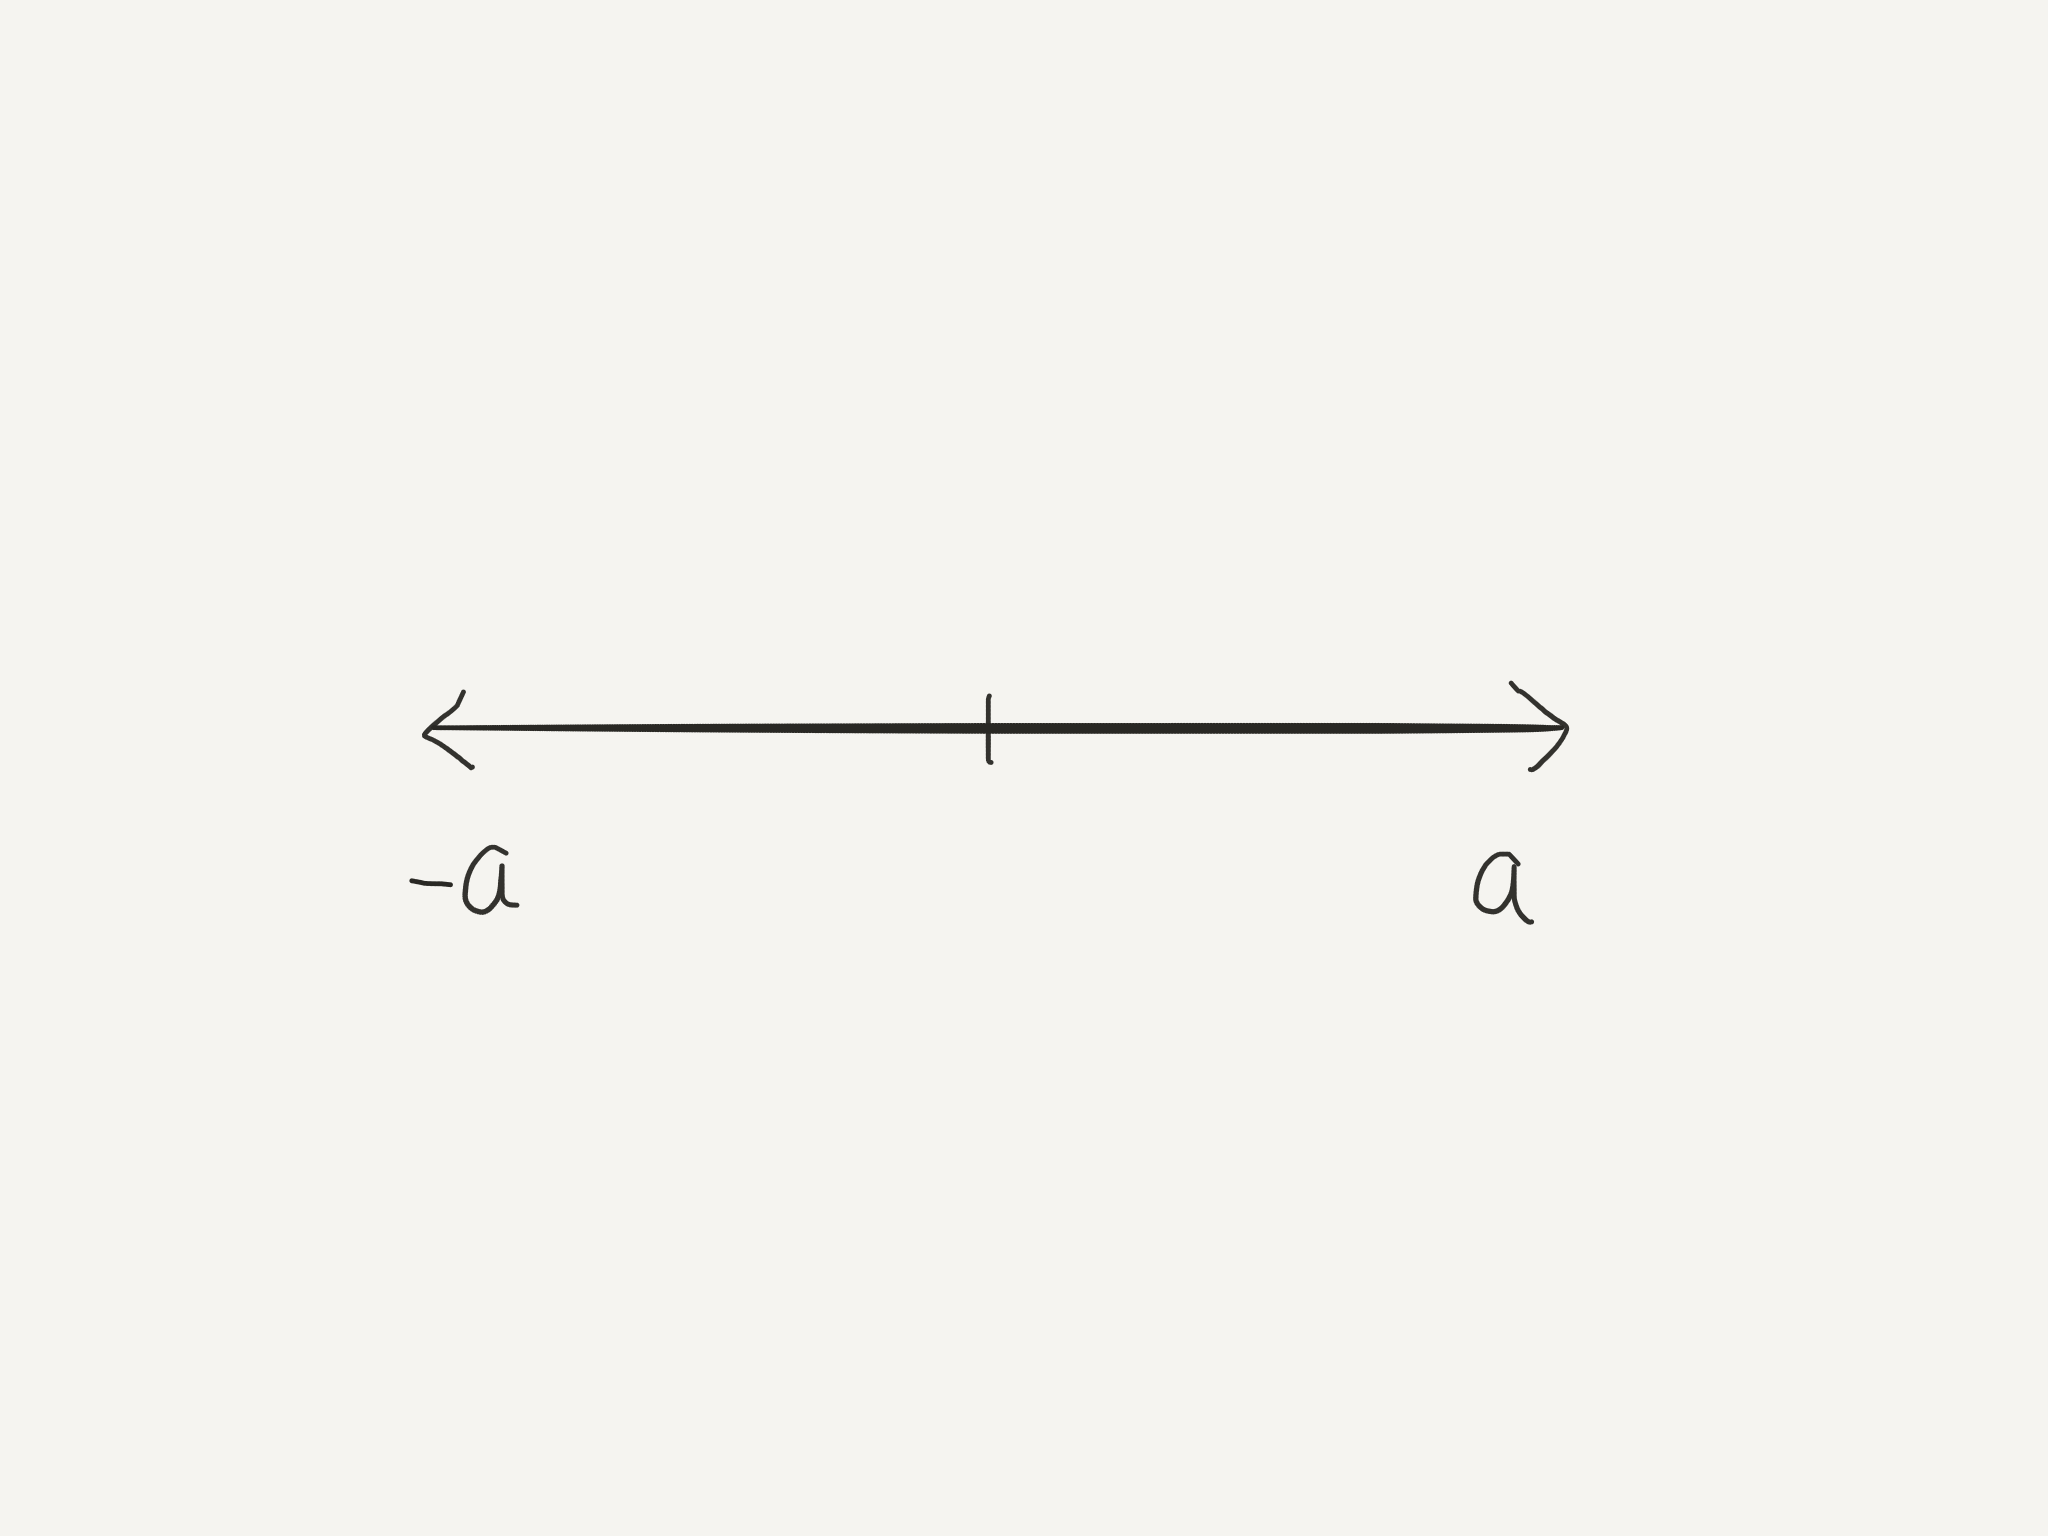
\includegraphics[scale=.15]{249-7.png}
\]
(with $a^{\vee}$ uniquely determined by the condition $a^{\vee}(a) = 2$); this is denoted A$_1$.
Are there any others (up to isomorphism)? Suppose we tried to add another root $b \ne \pm a$, 
so $\Phi$ must contain $\{-b,-a,a,b\}$. We may and do assume (by relabeling if necessary)
that $b = q a$ for some $q \in \Q$ with $q > 1$.  This is usually not contained in any root system:
\[
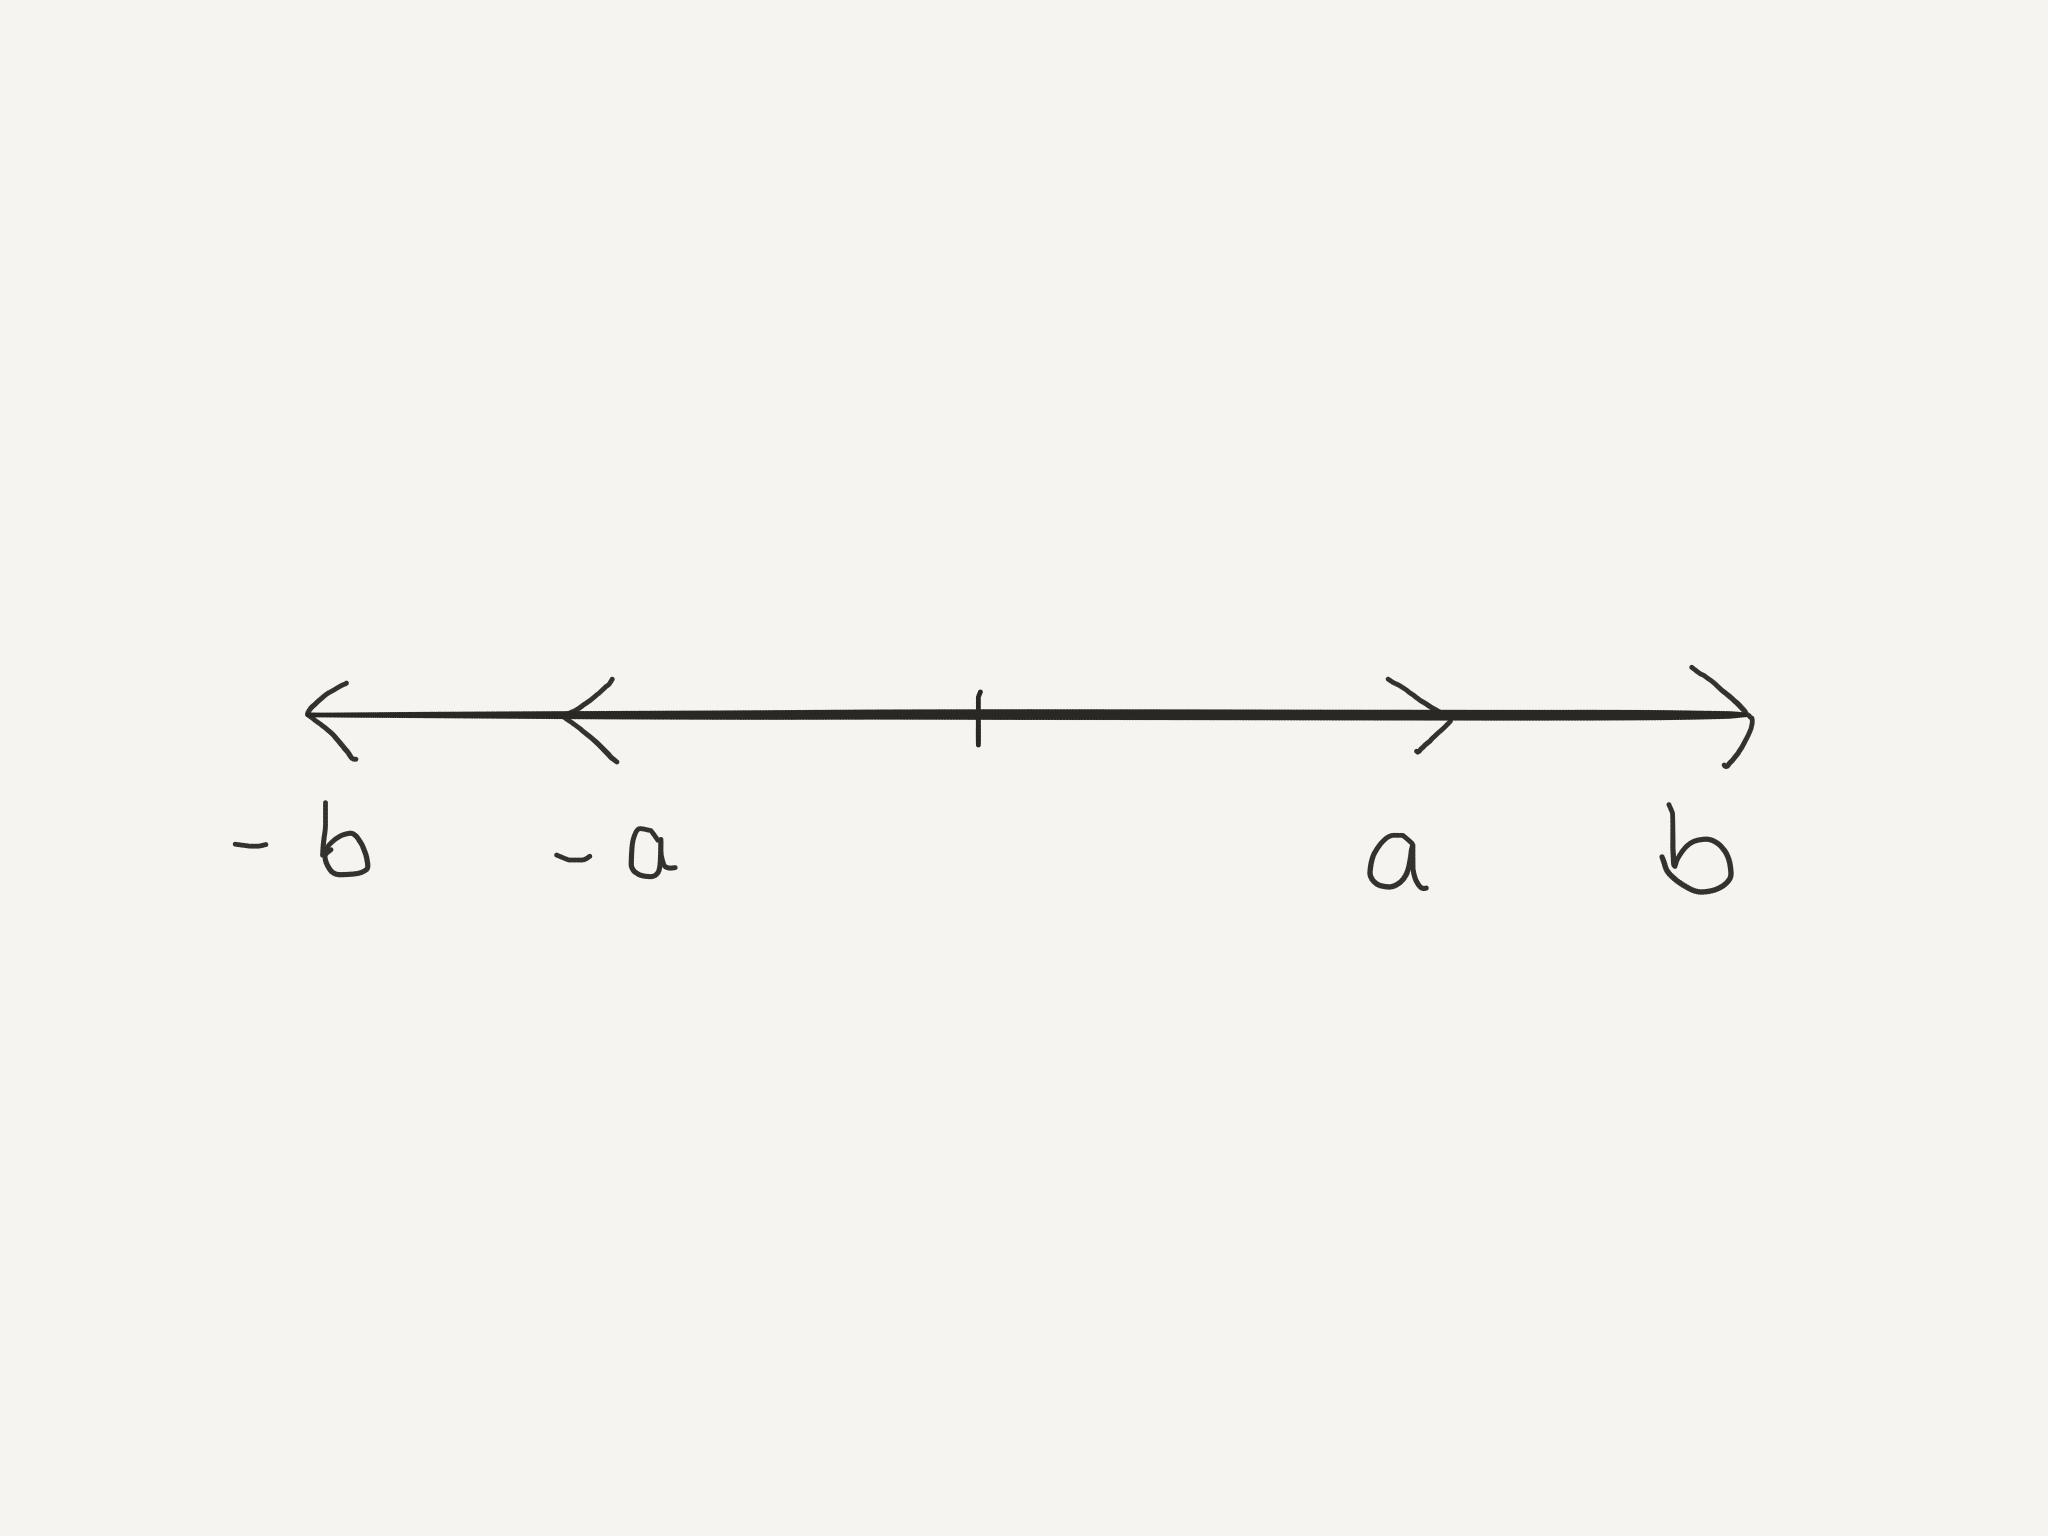
\includegraphics[scale=.15]{249-8.png}
\]
the second condition in the definition is not a problem since reflections in dimension 1 are simply negation, but
the first condition implies
\begin{align*}
\langle a^{\vee}, a \rangle &= 2 \\
\langle a^{\vee}, b \rangle & \in \Z\\
\langle b^{\vee}, b \rangle &= 2 \\
\langle b^{\vee}, a \rangle & \in \Z
\end{align*}
Writing $b = qa$ with $q > 1$, we have $2q \in \Z$, $b^{\vee} = (1/q)a^{\vee}$, and $2/q \in \Z$.
Hence, $q = n/2$ for some integer $n > 2$ such that $2/q = 4/n$ is an integer, so $n = 4$; i.e., $q = 2$.
In other words, there is exactly one other 1-dimensional root system, obtained by taking $b=2a$
(and it cannot be made any larger); this is called BC$_1$ and it is non-reduced.
\end{example}

\begin{example}
The reduced 2-dimensional root systems are ${\rm{A}}_1 \times {\rm{A}}_1, 
{\rm{B}}_2={\rm{C}}_2, {\rm{A}}_2, {\rm{G}}_2$. 
\[
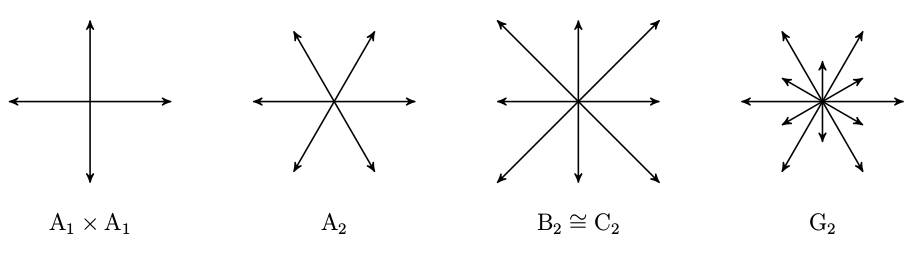
\includegraphics[scale=.4]{249-9.png}
\]
These are all \emph{reduced}. There is a unique non-reduced root system including ${\rm{B}}_2 =
{\rm{C}}_2$, 
called BC$_2$ (it is the union of a copy of B$_2$ and a copy of C$_2$ for which the short roots
of a copy of C$_2$ are the long roots of a copy of B$_2$), and the only other non-reduced 2-dimensional root systems turn out
to be ${\rm{A}}_1 \times {\rm{BC}}_1$ and ${\rm{BC}}_1 \times {\rm{BC}}_1$. 
\begin{figure}
\centering
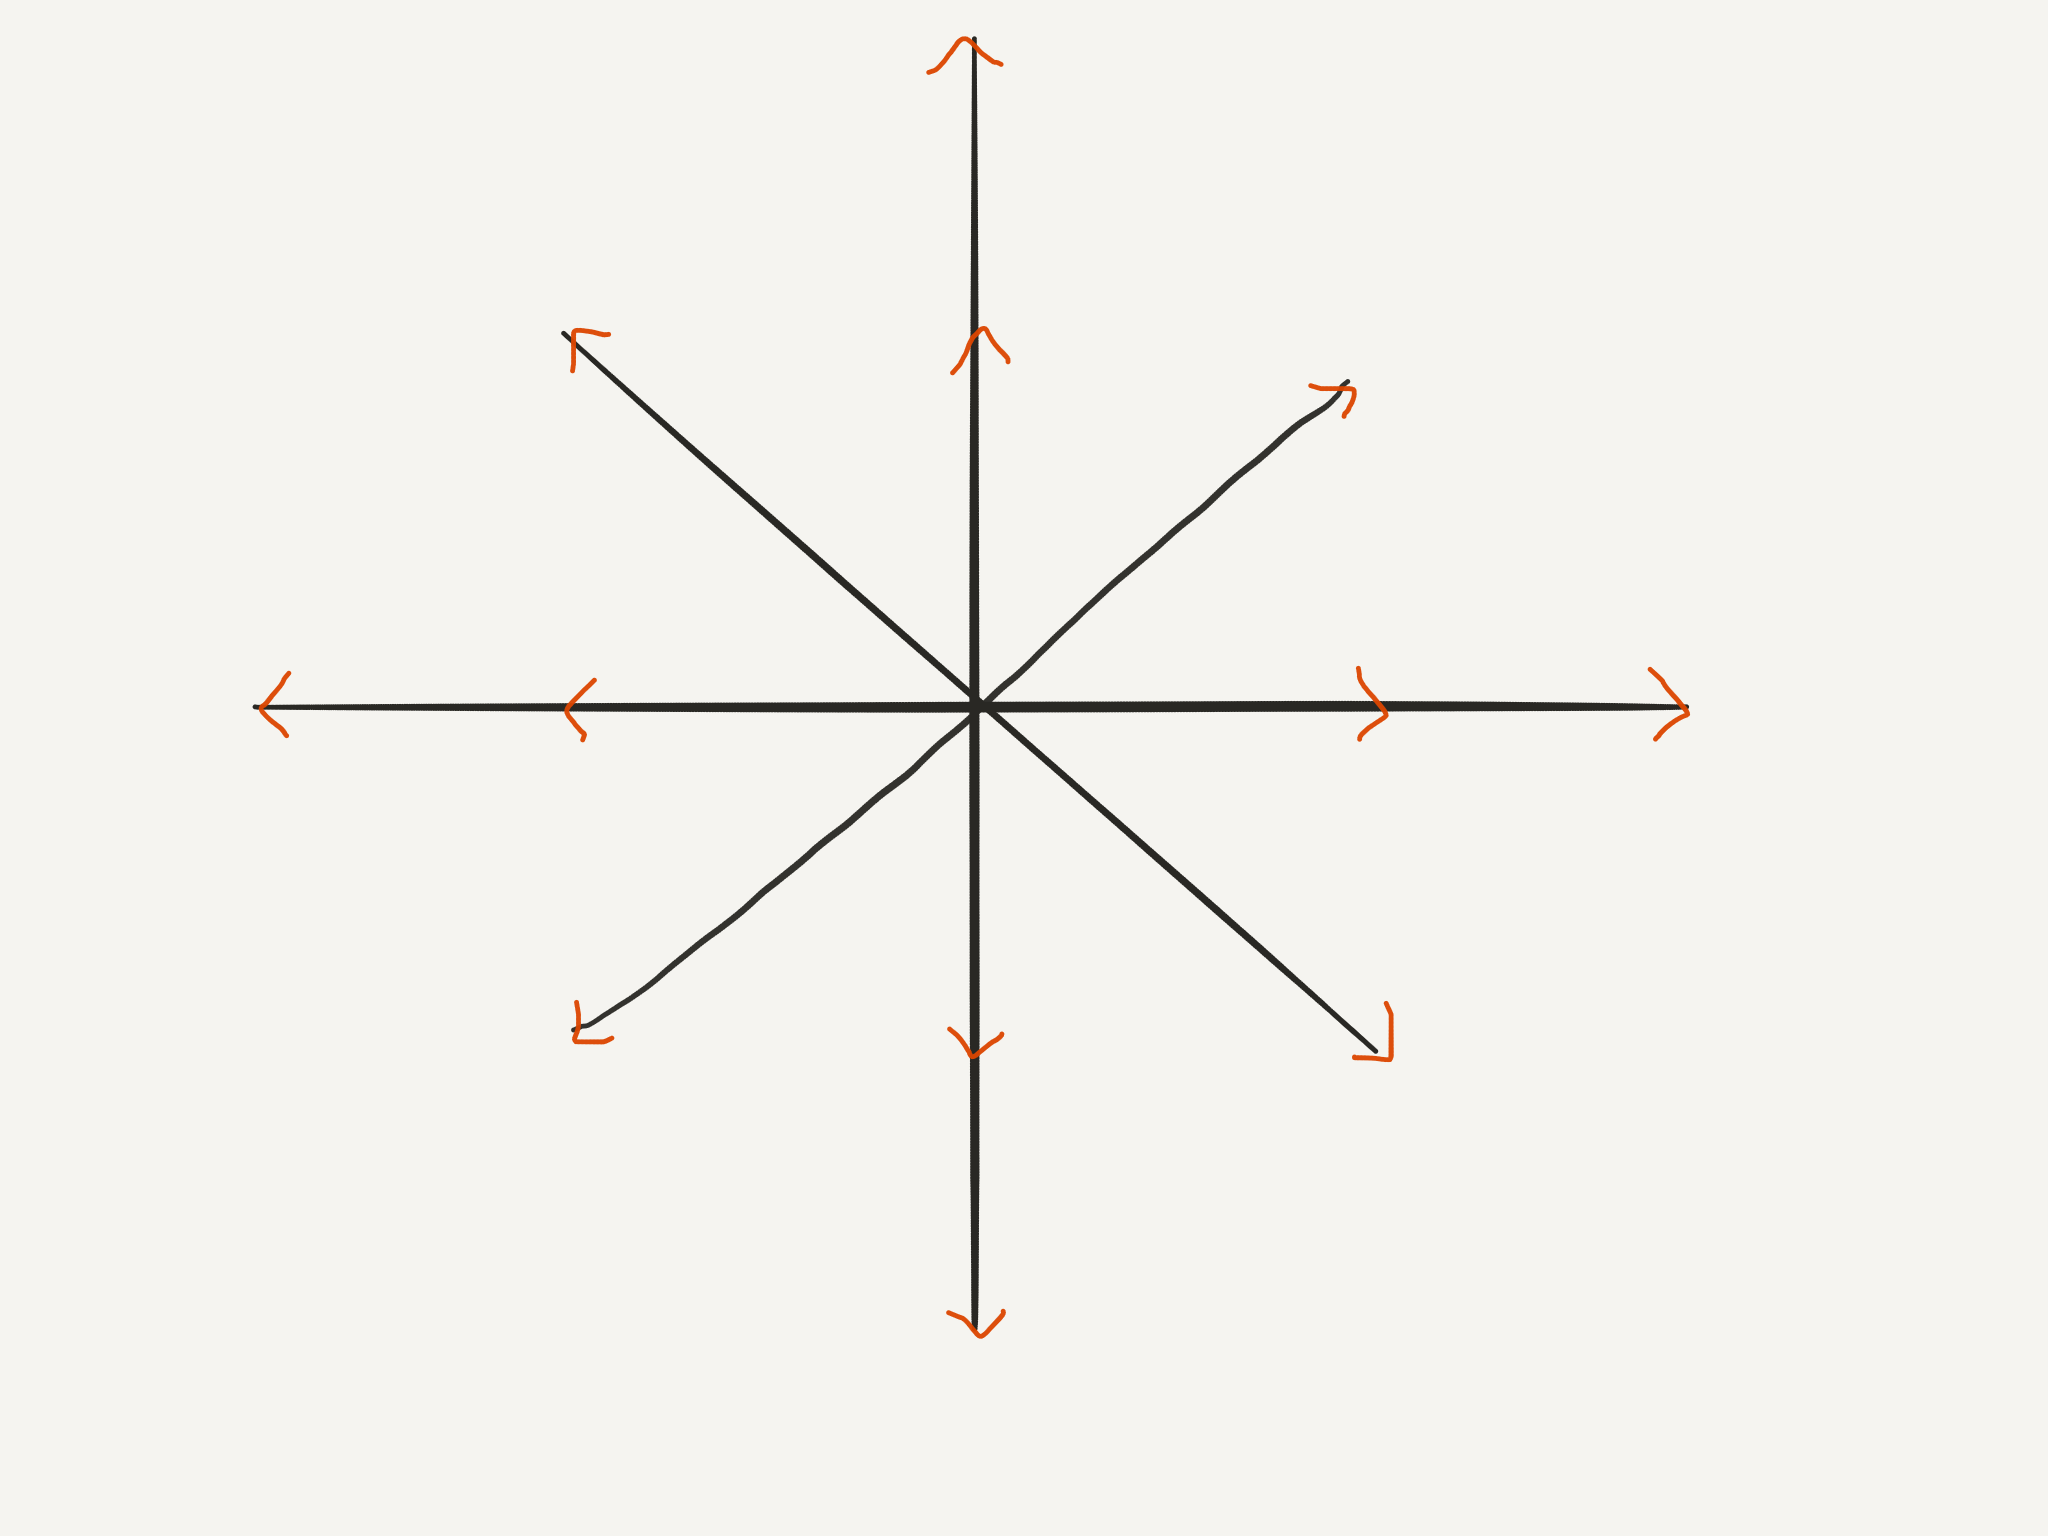
\includegraphics[scale=.2]{249-10.png}
\caption{Nonreduced root system of rank 2.}
\end{figure}
\end{example}

\begin{remark}
It is not immediate from the definition, but $a \mapsto a^{\vee}$ is well-defined; i.e. $a^{\vee}$ is {\em uniquely} determined by $a$. 
%The reason is as follows.
%As for any representation of a finite group over $\R$,
% one can put a Euclidean structure on $V_{\R}$ such that all the reflections are orthogonal. 
% We call a root system$(V, \Phi)$ {\em irreducible} if it is not $(0, \emptyset)$ 
% and is not a direct product of lower-dimensional root systems. 
% It is a general fact (which we will discuss later) that $(V, \Phi)$ is irreducible if and
% only if $V_{\R}$ is absolutely irreducible as a representation of the group generated by the reflections,
%so the Euclidean structure is unique up to a scalar.  Consequently,
%the line orthogonal to $\ker a^{\vee}_{\R}$ relative to this Euclidean structure is {\em uniquely}
%determined, so the condition $a^{\vee}(a) = 2$ expressing that $r_{a, a^{\vee}}(a) = -a$
%uniquely pins down the vector in that orthogonal line 
%, and $a^{\vee}$ is determined by demanding that $r_{a, a^{\vee}}$ be orthogonal. 
See \cite[XXI, 1.1.4]{SGA3} for a self-contained proof of this fact.
Therefore, we can write $r_a := r_{a, a^{\vee}}$.  Since $r_a$ and $a$ uniquely
determined the linear form $a^{\vee}$, it follows that $\Phi \rightarrow V^{\ast}$
defined by $a \mapsto a^{\vee}$ is a bijection onto a finite subset of $V^{\ast} - \{0\}$
denoted $\Phi^{\vee}$. It turns out that $(V^{\ast}, \Phi^{\vee})$ is a root system,
called the {\em dual} of $(V, \Phi)$. Elements of $\Phi^{\vee}$ are called {\em coroots}. 
\end{remark}

In Appendix \ref{rootdatum} 
it is shown that the roots of a split connected semisimple group form
a root system.  (A more refined result is proved there involving the notion of {\em root datum},
which we will discuss this later.) Let's explain where the coroots come from
in group-theoretic terms. 

Let $G$ be a connected semisimple group over a field $k$ and suppose it
contains a split maximal $k$-torus $T$, so
\[
V := {\rm{X}}(T)_{\Q} \supset \Phi(G,T) =: \Phi.
\]
For $a \in \Phi$, we seek $a^{\vee} \in V^{\ast} = {\rm{X}}_{\ast}(T)_{\Q}$ whose pairing
with all roots is in $\Z$.  We will find $a^{\vee}$ inside ${\rm{X}}_{\ast}(T)$ (even when $\Z \Phi$ is a proper
sublattice of ${\rm{X}}(T)$). To get started, $a$ corresponds to a $k$-homomorphism
\[
a \colon T \rightarrow \G_m.
\]
For the torus $T_a := \ker(a)_{\red}^0$ of codimension-1 in $T$,
the connected reductive $k$-group $Z_G(T_a)$
contain $T$ as a split maximal $k$-torus
and $T_a$ is central. 
In fact, $T_a$ is the {\em maximal} central $k$-torus in $Z_G(T_a)$ since the maximal
$k$-torus $T$ of dimension $1 + \dim T_a$ is non-central in $G_a$, 
as its action on ${\rm{Lie}}(Z_G(T_a)) = \mathfrak{g}^{T_a}$ supports
root lines for $\pm a$. 

Hence, for $G_a := \mathscr{D}(Z_G(T_a))$, multiplication $T_a \times G_a \rightarrow Z_G(T_a)$
is a central isogeny with $G_a$ connected semisimple of rank $1$
having $$\mathscr{T}_a := T \cap G_a$$
as a {\em split} maximal $k$-torus. (Recall the general link between maximal tori
of a connected reductive group and of its derived group; apply that to $Z_G(T_a)$.) Hence, 
by the classification of rank one semisimple groups (from the previous course), 
$G_a \simeq \SL_2$ or $\PGL_2$ carrying $\mathscr{T}_a$
over to the diagonal $k$-torus.

We will find a $k$-homomorphism $a^{\vee} \colon \G_m \rightarrow \mathscr{T}_a \subset T$
which does the job. Since $a:T \rightarrow \G_m$ is nontrivial and kills $T_a$, the restriction
$a|_{\mathscr{T}_a}$ to the canonical isogeny-complement torus $\mathscr{T}_a$ to $T_a$ inside $T$
is nontrivial. 
But $\mathscr{T}_a$ is 1-dimensional (and split), so the desired 
$\mathscr{T}_a$-valued cocharacter $a^{\vee}$ is uniquely determined (if it exists!)
by the requirement $\langle a, a^{\vee} \rangle = 2$.  This uniqueness enables us to make
some choices in the construction of $a^{\vee}$ without any concern that the end result will depend on choices
beyond $(G, T, a)$. 

To build such an $a^{\vee}$, we treat separately the cases that $G_a$ is SL$_2$ or PGL$_2$.
\begin{itemize}
\item In the SL$_2$-case, fix an isomorphism $G_a \simeq {\rm{SL}}_2$
carrying $\mathscr{T}_a$ over to the diagonal torus $\{(\begin{smallmatrix} t & 0 \\ 0 & 1/t \end{smallmatrix})\}$.
This isomorphism must carry the $\mathscr{T}_a$-root group $U_a \subset G_a$ over
to one of the two root groups $U^{\pm}$ in ${\rm{SL}}_2$ for the diagonal torus. 
We may conjugate the chosen isomorphism $G_a \simeq {\rm{SL}}_2$ against the standard Weyl element
$w = (\begin{smallmatrix} 0 & 1 \\ -1 & 0 \end{smallmatrix})$ if necessary
so that $U_a$ is carried over to $U^+$. Hence, 
the root $a|_{\mathscr{T}_a}$ computing the $\mathscr{T}_a$-action on
${\rm{Lie}}(G_a) = \mathfrak{sl}_2$ is the root $(\begin{smallmatrix} t&0\\0&1/t\end{smallmatrix})
\mapsto t^{2}$ for $U^+$.
Then we can write down the 1-parameter subgroup $a^{\vee}$ explicitly as
\[
t \mapsto \begin{pmatrix} t & 0 \\ 0 & t^{-1} \end{pmatrix}, 
\]
so $a^{\vee}: \G_m \rightarrow \mathscr{T}_a$ is an {\em isomorphism} in the SL$_2$-case. 

\item In the PGL$_2$-case we proceed similarly, the only difference being that 
the diagonal torus is described in terms of matrices
$(\begin{smallmatrix} t & 0 \\ 0 & 1 \end{smallmatrix})$ for which the corresponding
conjugation on $U^+$ induces multiplication by $t$ on the $k$-line ${\rm{Lie}}(U^+)$. 
Consequently,  $a^{\vee}: \G_m \rightarrow \mathscr{T}_a$ is a degree-2 isogeny
corresponding to $t \mapsto (\begin{smallmatrix} t^2&0\\ 0 & 1 \end{smallmatrix})$
since we require $\langle a, a^{\vee} \rangle=2$.
\end{itemize}

Since $T = T_a \cdot \mathscr{T}_a$ with $T_a$ central in $Z_G(T_a)$ and 
${\rm{Aut}}(\mathscr{T}_a) = \{\pm 1\}$, we have naturally
$$W(G_a, \mathscr{T}_a) \subset W(G, T) \subset {\rm{GL}}({\rm{X}}(T)) \subset
{\rm{GL}}({\rm{X}}(T_a)_{\Q} \oplus {\rm{X}}(\mathscr{T}_a)_{\Q})$$
as a subgroup of $\GL({\rm{X}}(T_a)) \times \GL({\rm{X}}(\mathscr{T}_a)) = \GL({\rm{X}}(T_a)) \times \{\pm 1\}$
with trivial effect on ${\rm{X}}(T_a)$.  That is, $W(G_a, \mathscr{T}_a)$ has order at most 2, as its
elements induces the identity 
on the hyperplane ${\rm{X}}(T_a)_{\Q} = (\ker a^{\vee})_{\Q}$ and induce $\pm 1$
on the complementary line ${\rm{X}}(\mathscr{T}_a)_{\Q} = \Q \cdot a$ (!), 
so $W(G_a, \mathscr{T}_a)$ really has order exactly 2 since 
 conjugation against the standard 
Weyl element $w$ in SL$_2$ or PGL$_2$
identified with $G_a$ as above gives a nontrivial element. 

This nontrivial element is a reflection that {\em must} be 
the canonical refection $r_a$ on ${\rm{X}}(T)_{\Q}$ since both
automorphisms of ${\rm{X}}(T)_{\Q}$ satisfy the {\em same} properties. 
In other words, $r_a$ is also characterized uniquely as being the only nontrivial
element in $W(G_a, \mathscr{T}_a)$. 

\begin{remark}
As an element of $N_{G_a}(\mathscr{T}_a)(k)$ rather than merely its
quotient $W(G_a, \mathscr{T}_a)$ we do {\em not} get a canonical element. Indeed, it is 
ambiguous up to translation by $\mathscr{T}_a(k)$, precisely the ambiguity in the choice
of isomorphism from $G_a$ onto SL$_2$ or PGL$_2$ carrying $\mathscr{T}_a$ onto
the diagonal torus and $U_a$ onto $U^+$.  Note also that if ${\rm{char}}(k) \ne 2$ then the standard Weyl element
in SL$_2(k)$ has order 4 rather than order 2. 
\end{remark}

\subsection{Parabolic sets of roots}\label{parrootsec}

Given $\Phi \supset \Psi = \Phi(P,T)$ we want to find $\lambda \in {\rm{X}}_*(T)_{\Q}$ such that $\Phi_{\lambda \geq 0} = \Psi$. We need to find an \emph{intrinsic} characterization of subsets of $\Phi$ of the form $\Phi_{\lambda \geq 0}$, mirroring the one for parabolics as subgroups containing a Borel.

\begin{definition} For a root system $\Phi$, 
a subset $\Psi \subset \Phi$ is called \emph{closed} if for all $a, b \in \Psi$ such that $a+b \in \Phi$, we also have $a+b \in \Psi$. 
\end{definition}

\begin{example}
Subsets of the form $\Phi_{\lambda \geq 0}$ and $\Phi_{\lambda > 0}$ (for $\lambda \in V^{\ast}$),
or more generally $\Phi \cap A$ for a subsemigroup $A \subset V$, are closed.
\end{example}

This condition isn't enough to characterize subsets of the form $\Phi_{\lambda \geq 0}$, since (for instance) the latter contain at least half of the roots. (Recall $\Phi \subset V - \{0\}$ is a finite subset stable under negation.) 

\begin{definition}
A subset $\Psi$ of a root system$\Phi$ is {\em parabolic} if 
\begin{enumerate}
\item $\Psi$ is closed, 
\item $\Psi \cup (-\Psi) = \Phi$. 
\end{enumerate}
\end{definition}

\begin{example}
For $\lambda \in {\rm{X}}_*(T)$, $\Phi_{\lambda \geq 0}$ is a parabolic subset. 
\end{example}

\begin{proposition}\cite[Prop.\,2.2.8]{pred}\label{228} 
Any parabolic subset of a root system $\Phi$ is of the form $\Phi_{\lambda \geq 0}$ for some $\lambda \in V^{\ast}$.
\end{proposition}

The proof (given in \cite{pred}) is an application of the early developments about root
systems in  \cite[VI, \S1.7]{bourbaki}. 
Here we just  give an intuitive explanation for how to find $\lambda$, given a parabolic subset. First consider the case $\Psi \cap (-\Psi) = \emptyset$, so the parabolic set $\Psi$ 
is a closed subset consisting of \emph{exactly} half of the roots. In this case we 
seek $\lambda$ that is regular (since $\Phi_{\lambda \ge 0}$ will need to be disjoint
from its negative). 

We need to appeal to the theory of ``bases'' of
root systems. A {\em basis} of $\Phi$ is a subset $\Delta$ with two properties:
\begin{itemize}
\item $\Delta$ is a basis for $V$, 
\item every element of $\Phi$ has its $\Delta$-coefficients either all in $\Z_{\ge 0}$ or all in $\Z_{\le 0}$.
\end{itemize}
\begin{figure}

\centering
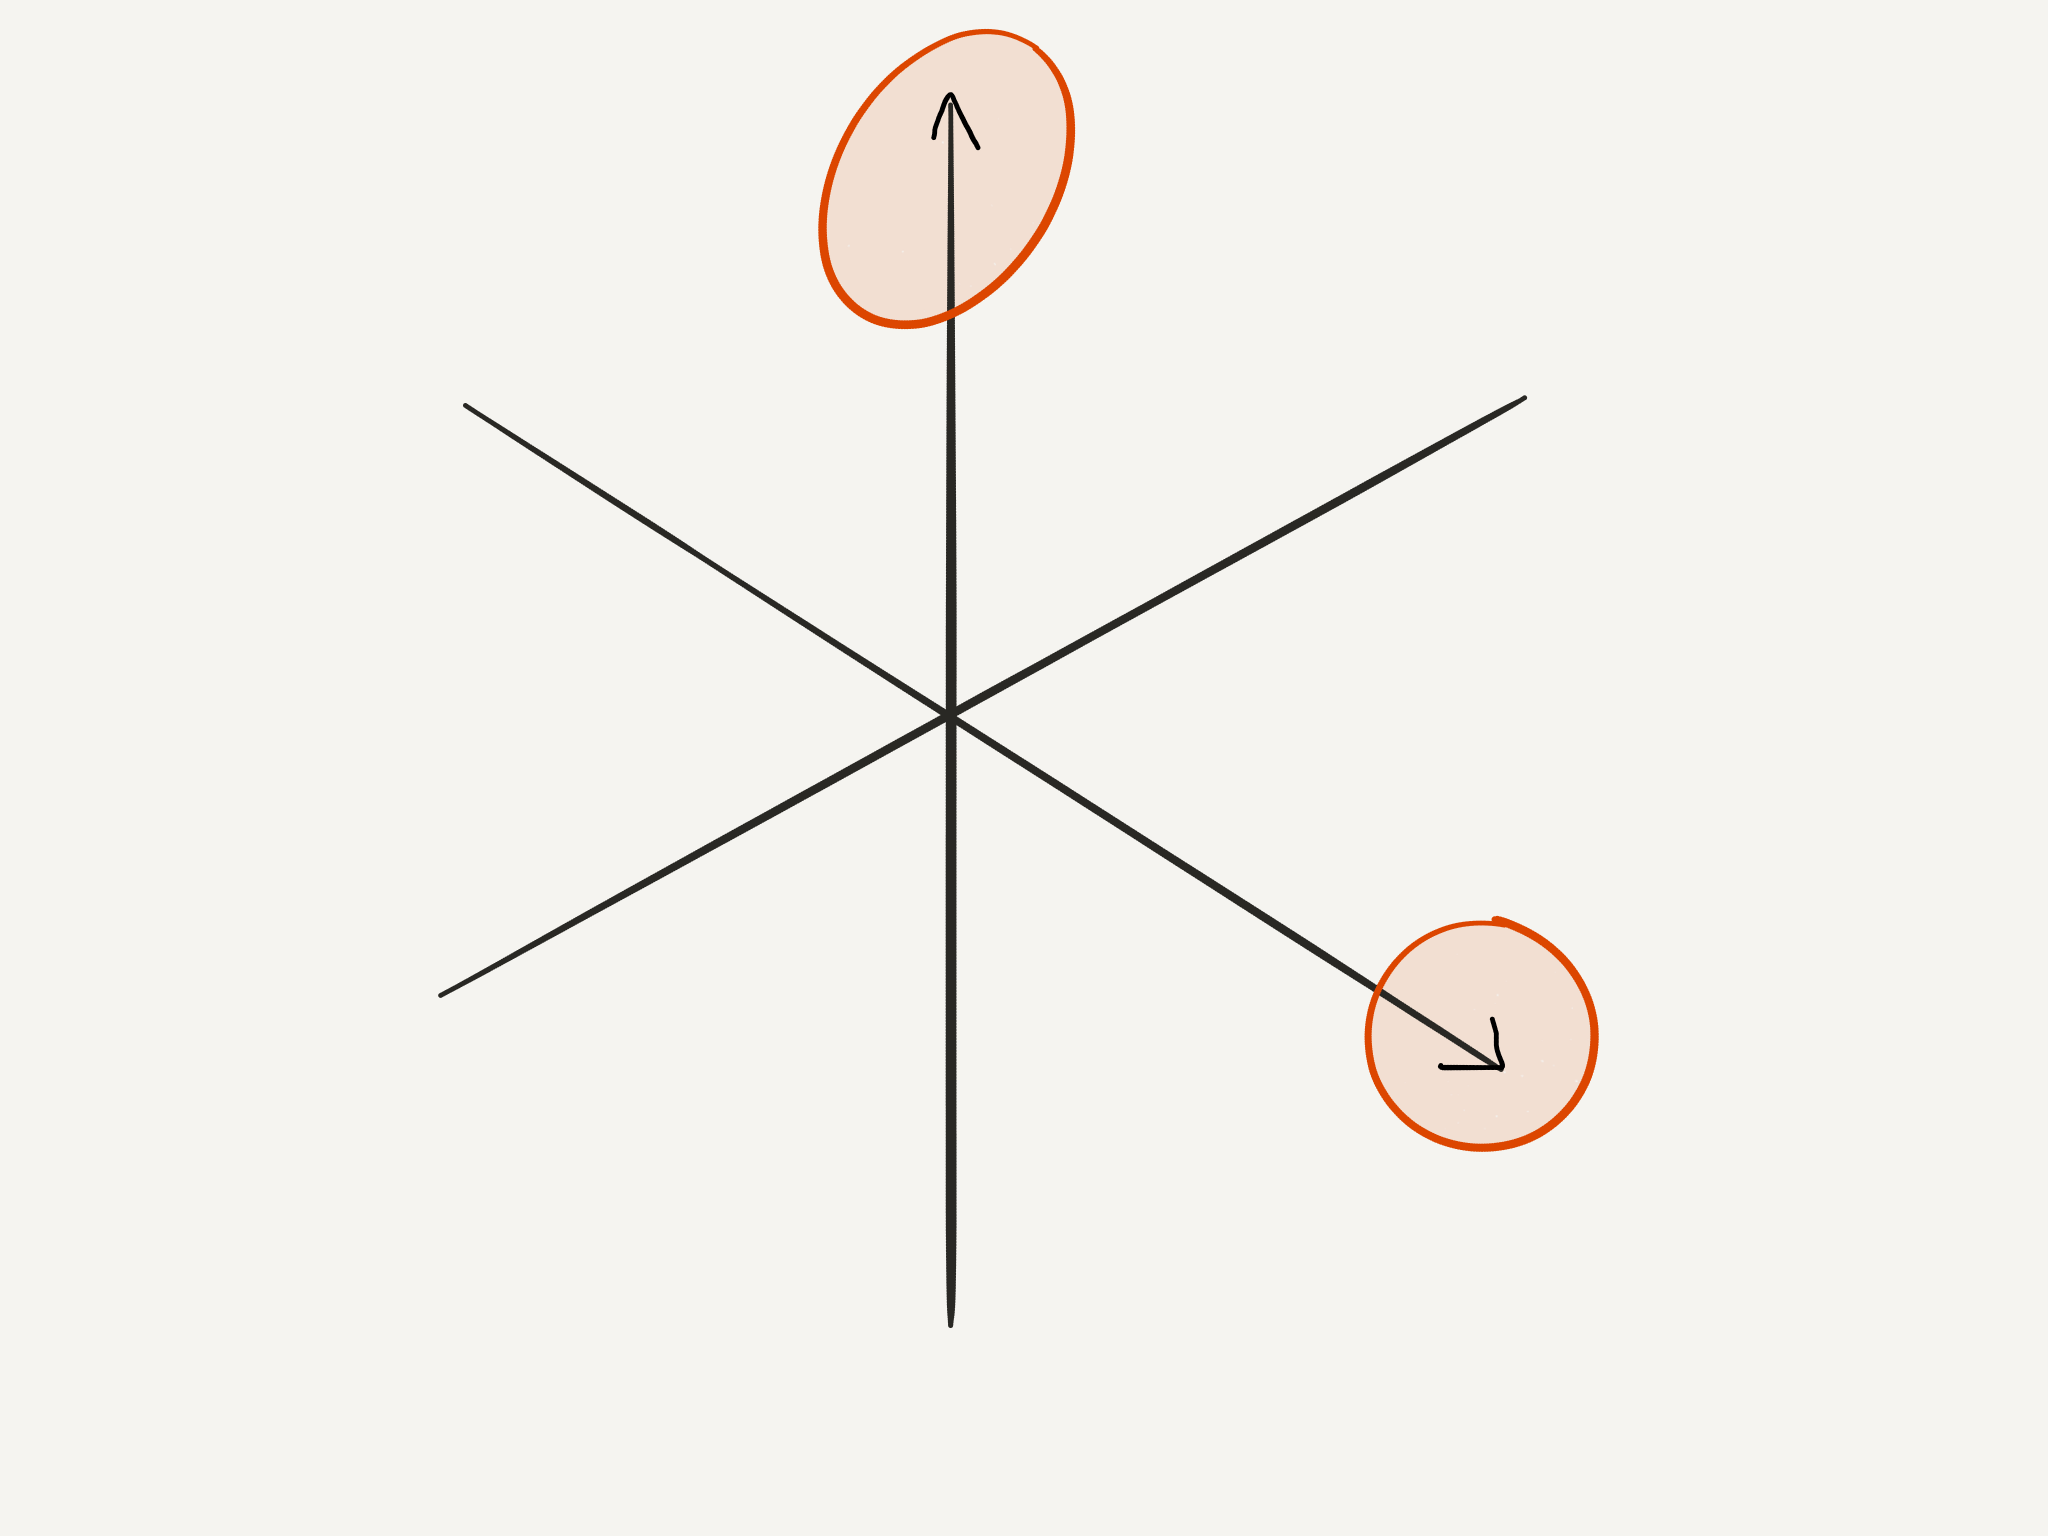
\includegraphics[scale=.2]{249-11.png}
\caption{A basis for the root system $A_2$.}
\end{figure}

The general fact is that for any parabolic subset 
there exists a basis $\Delta$ of $\Phi$ such that the parabolic subset contains
$(\Z_{\ge 0} \Delta) \cap \Psi$.
(This is the counterpart 
of the characterization of parabolic subgroups of
connected reductive groups over algebraically closed
fields as smooth closed subgroups contains a Borel subgroup.)
For any basis $\Delta$ of $\Phi$ we get the dual $\Q$-basis $\Delta^* =\{b^*\}_{b \in \Delta}$ 
of $V^*$. 

\begin{remark}[Warning]
Do not confuse $b^*$ with $b^{\vee}$; they are not equal in general! Indeed, we can have 
$\langle a, b^{\vee} \rangle \ne 0$ for linearly independent $a, b \in \Delta$,
as already happens for B$_2$ and G$_2$, whereas by design $\langle a, b^{\ast} \rangle = 0$
for distinct $a, b \in \Delta$.
\end{remark}

Returning to a parabolic $\Psi$ of exactly half the size of $\Phi$, define $\lambda = \sum_{b \in \Delta} b^*$
for $\Delta$ whose non-negative $\Z$-linear combinations in $\Phi$ are contained in $\Psi$, and hence
coincide with $\Psi$ by counting reasons.
This works precisely from the definition of $\Delta$ being
a basis contained in $\Psi$.

If instead $\Psi \cap (-\Psi)$ is non-empty,
consider $\Phi' = \Psi \cap (-\Psi)$. It turns out that this is also a root system in its own $\Q$-span
inside $V$. (The image
of $\Phi$ in the quotient $V/(\Q\cdot \Phi')$ may not be a root system.) The idea is to find a basis $\Delta' \subset \Phi'$ and extend it to a basis $\Delta$ of $\Phi$ contained in $\Psi$. 
Then one takes $\lambda = \sum_{b \in \Delta - \Delta'} b^*$. 

We finish the proof of Theorem \ref{pardyn} by proving: 

\begin{proposition} Let $G$ be a connected semisimple group over $k = \overline{k}$. 
If $P \subset G$ is a parabolic subgroup and $T \subset P$ is a maximal torus
then the subset $\Psi := \Phi(P, T) \subset \Phi(G,T)$ is parabolic.
\end{proposition}

Since $P$ contains a Borel subgroup $B$ and the $T$-roots occurring
in ${\rm{Lie}}(B)$ cover $\Phi$ up to signs, clearly $\Psi \cup (-\Psi) = \Phi$. Hence, by Proposition \ref{228}, it 
remains to check that $\Psi$ is closed.  This will rest on a general
criterion for closedness of a subset of a {\em reduced} root system in terms of reflections, the proof of which 
involves calculations with (reduced) rank-2 root systems. 


Let $G$ be a connected \emph{semisimple} group over $k  = \ol{k}$, $P \subset G$ a parabolic group, 
and $T$ a maximal torus inside $P$. Note that ${\rm{X}}(T)_{\Q} = \Q \cdot \Phi$ since
$\Z \Phi$ has finite index inside ${\rm{X}}(T)$ in the semisimple case.  We need to show that 
the subset $\Phi(P, T) \subset \Phi := \Phi(G, T)$ is closed. We know that $P \supset B \supset T$ for a Borel subgroup $B = P_G(\mu)$ for some regular cocharacter $\mu \in {\rm{X}}_*(T)$. Therefore, 
\[
\Phi(P,T) \supset \Phi^+ := \Phi(B,T) = \Phi_{\mu \geq 0} = \Phi_{\mu>0}. 
\]
We shall use the following sufficient criterion for a subset of roots in a {\em reduced}
root system (such as $\Phi(G, T)$) to be closed:

\begin{proposition}\label{closed_crit}
Let $(V,\Phi)$ be a reduced root system. A subset $\Psi \subset \Phi$ containing $\Phi_{\mu >0}$ for a regular cocharacter $\mu$ is closed if for all $\{c, -c\} \subset \Psi$ the action of 
the reflection $r_c$ on $\Phi$ preserves $\Psi$. 
\end{proposition}

We'll prove this soon using case-checking for all rank-2 reduced root systems (${\rm{A}}_1 \times 
{\rm{A}}_1$, ${\rm{A}}_2$, ${\rm{B}}_2={\rm{C}}_2$, ${\rm{G}}_2$). But first let's see how to use 
this criterion. For root systems coming from an actual split reductive
pair $(G, T)$, the reflections come from the standard
Weyl element in $\SL_2$ or $\PGL_2$ identified with $G_c = \langle U_c, U_{-c} \rangle =
\mathscr{D}(Z_G(T_c)) \subset G$ (equipped with the split maximal torus $\mathscr{T}_c := T \cap G_c$). 
So in that setting for $\Psi = \Phi(P, T)$ it suffices to show that such Weyl elements arise from $P(k)$
when $\{c, -c\} \subset \Psi$.   The key claim is:

\begin{lemma}\label{puc} If $c \in \Phi(P,T)$ then $U_c \subset P$. 
\end{lemma}

Granting this lemma, it follows that if $\{c,-c\} \subset \Phi(P,T)$ then 
\[
P \supset \langle U_c, U_{-c} \rangle = G_c := \Cal{D}(Z_G(T_c)) \simeq \SL_2 \text{ or }\PGL_2
\]
where the final isomorphism carries the split maximal $k$-torus $\mathscr{T}_c := T \cap G_c$
over to the diagonal. Then $P$ contains the $k$-point $n_c$ corresponding to $(\begin{smallmatrix} 0 & 1 \\ -1 & 0\end{smallmatrix})$ in $\SL_2$ or $\PGL_2$, and $n_c$-conjugation preserves $T_c \cdot \Cal{T}_c = T$ (as the identity on $T_c$ and $-1$ on $\Cal{T}_c$), inducing $r_c$ on ${\rm{X}}(T)$. Since conjugation on
$G$ by $n_c \in P(k)$ trivially preserves $P$ (and $T$), it follows that the induced effect
$r_c$ of $n_c$-conjugation on ${\rm{X}}(T)$ preserves $\Phi(P, T)$ as desired.  Here is the proof of Lemma \ref{puc}.

\begin{proof}
We have $P \supset B \supset T$, so 
\[
Z_P(T_c) = P \cap Z_G(T_c) \supset B \cap Z_G(T_c).
\]
Now, $Z_P(T_c) $ is smooth and connected and $B \cap Z_G(T_c)$ is a Borel subgroup of $Z_G(T_c)$
(recall that intersecting a Borel subgroup with the centralizer of a subtorus of the Borel
always yields a Borel subgroup of that torus centralizer), so $P \cap Z_G(T_c)$ is parabolic in $Z_G(T_c)$. 

We know that for any connected reductive group $H$, there is a natural bijection 
\[
\{\text{parabolics of $H$}\} \Longleftrightarrow \{\text{parabolics of $\Cal{D}H$} \}
\]
due to the central isogeny $Z \times \mathscr{D}(H) \rightarrow H$ for the maximal central torus $Z \subset H$
that is contained in every maximal torus and hence in every parabolic subgroup. Thus, the fact that 
 $P \cap Z_G(T_c)$ is \emph{parabolic} in $Z_G(T_c)$ implies that $P \cap G_c$ is parabolic in $G_c$.
 The (split) maximal torus $\Cal{T}_c \subset G_c$ acts on ${\rm{Lie}}(G_c)$ with the only roots being 
 $c|_{\mathscr{T}_c}$ and $-c|_{\mathscr{T}_c}$. Hence, we can pass to $G_c$ (and $\Cal{T}_c$) to reduce to the case of $\SL_2$ or $\PGL_2$ with diagonal $T$. In this case the possibilities for parabolic subgroups $P$ containing $T$
are   $G$, $B^+$, and $B^-$, so the containment $U_c \subset P$ follows by inspection. 
\end{proof}

\begin{proof}[Proof of Proposition \ref{closed_crit}] For reduced $(V, \Phi)$ and regular $\mu \in V^*$ and $\Phi_{\mu>0} \subset \Psi \subset \Phi$, we want to show that $\Psi$ is closed if $\Psi$ is $r_c$-stable for all $\{c, -c\} \subset \Psi$. 

Choose $a,b \in \Psi$ such that $a+b \in \Phi$. Note that $a$ and $b$ can't be dependent because 
$\Phi \cap \Q \cdot a = \{\pm a\}$ and $0, 2a \not\in \Phi$ by the reducedness of $\Phi$. 
Thus, $V' := \Q a + \Q b \subset V$ is a plane, containing the  finite 
spanning $\Phi' := (\Z a + \Z b) \cap \Phi \subset V' - \{0\}$. This is itself a reduced root system (using 
the coroots $\{c^{\vee}|_{V'}\}_{c \in \Phi'}$) since the reflection of a root $c'$ through 
a reflection $r_{c''}$ is an integral combination of $c'$ and $c''$. Using $\Psi' = \Psi \cap \Phi'$, 
the problem reduces to that of $(V', \Phi', \Psi', \mu|_{V'})$, so now our problem 
considered reduced root systems of rank 2.

But there is a classification of reduced root systems $(V, \Phi)$ equipped
with a choice of $\Phi^+ = \Phi_{\mu > 0}$ for regular $\mu \in V^{\ast}$, rather explicit in the rank-2 case.  
We will discuss this more fully later when we need to make more serious use of Dynkin diagrams
and related concepts, but for now we simply state the classification and then check each case.
Of course, we can also assume at least one of $a$ or $b$ is not contained in $\Phi^+$ or else
there is nothing to do (as $\Phi^+ \subset \Psi$ by hypothesis and obviously $\Phi^+$ is closed). 

The possibilities, as mentioned already, are ${\rm{A}}_1 \times 
{\rm{A}}_1$, ${\rm{A}}_2$, ${\rm{B}}_2={\rm{C}}_2$, ${\rm{G}}_2$.  The first case is irrelevant since
no two roots have sum equal to a root in that case.  For the other cases,
to be systematic one separately considers the cases $a \in \Phi^+$, $b \not\in \Phi^+$
and then $a, b \not\in \Phi^+$ (exhausting all possibilities since the task is symmetric in $a$ and $b$). 
Taking into account symmetries of a regular hexagon, the case of A$_2$ involves just two possibilities
for $\{a, b\}$ to check, each of which is easy, and to illustrate the more interesting case-checking we
now present the case of B$_2$.

\[
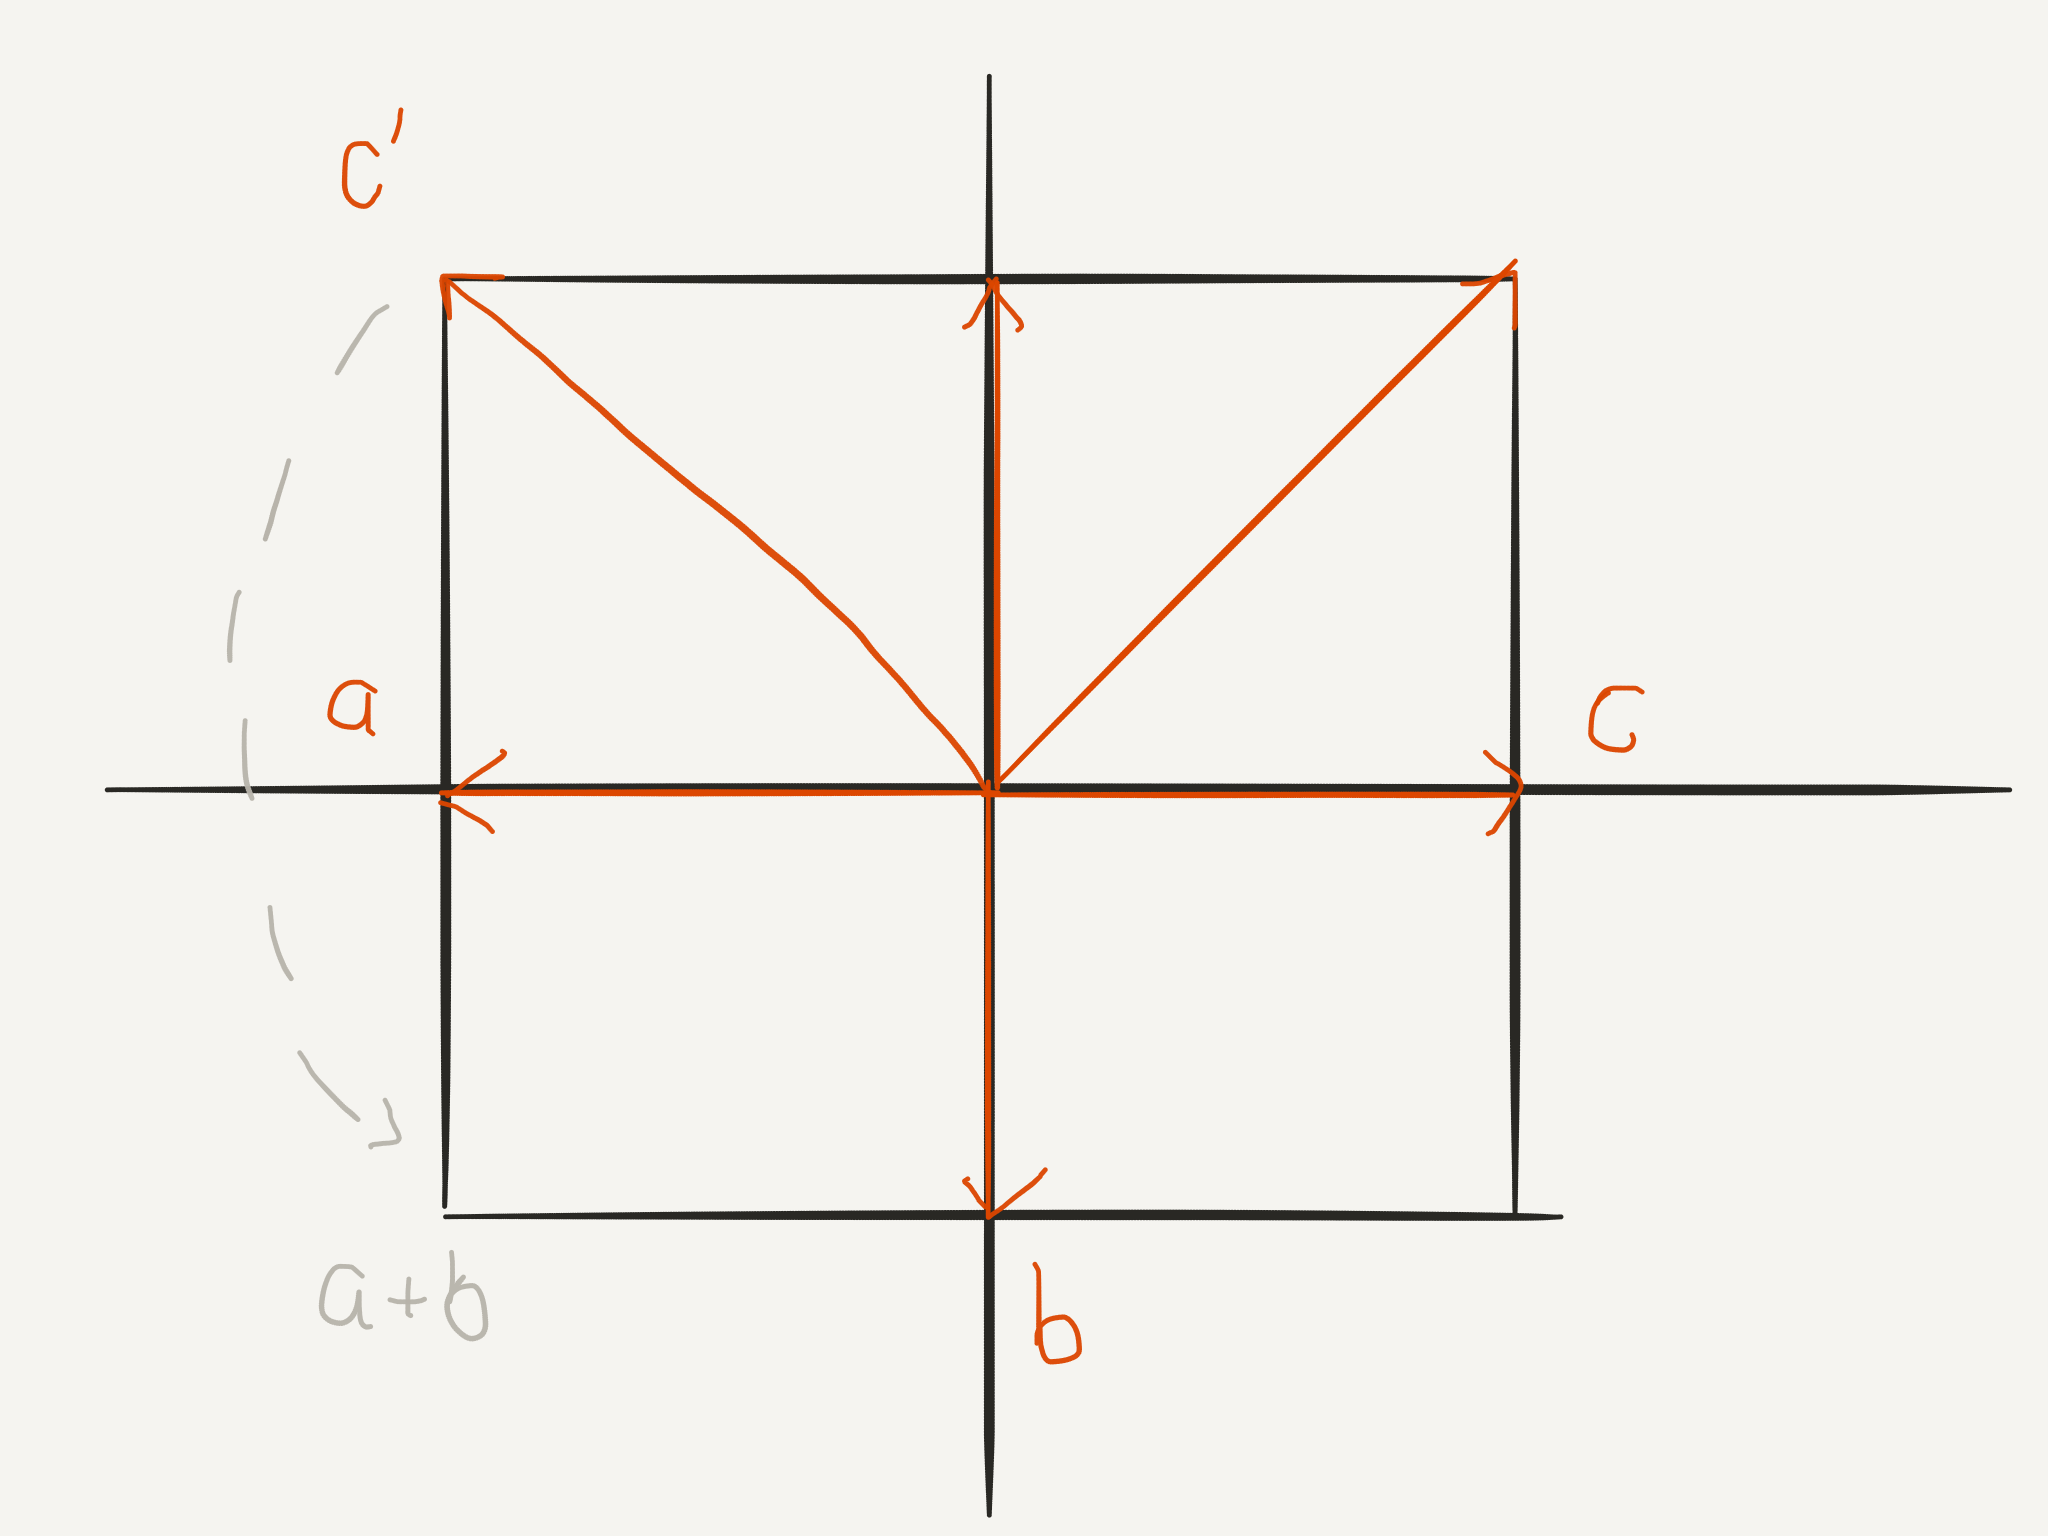
\includegraphics[scale=.2]{249-12.png}
\]
The above Figure is for one of the few cases to consider with $a, b \not\in \Phi^+$ (where $\Phi^+$ consists
of the $\Z_{\ge 0}$-linear combinations of $c$ and $c'$ as shown). We want to show that $a+b \in \Psi$. Since $b$ and $-b$ are in $\Psi$, we have by assumption that $r_b$ preserves $\Psi$. But then $a+b = r_b(c') \in \Psi$.  

Among the few cases with $a \in \Phi^+$ and $b \not\in \Phi^+$, here is one:
\[
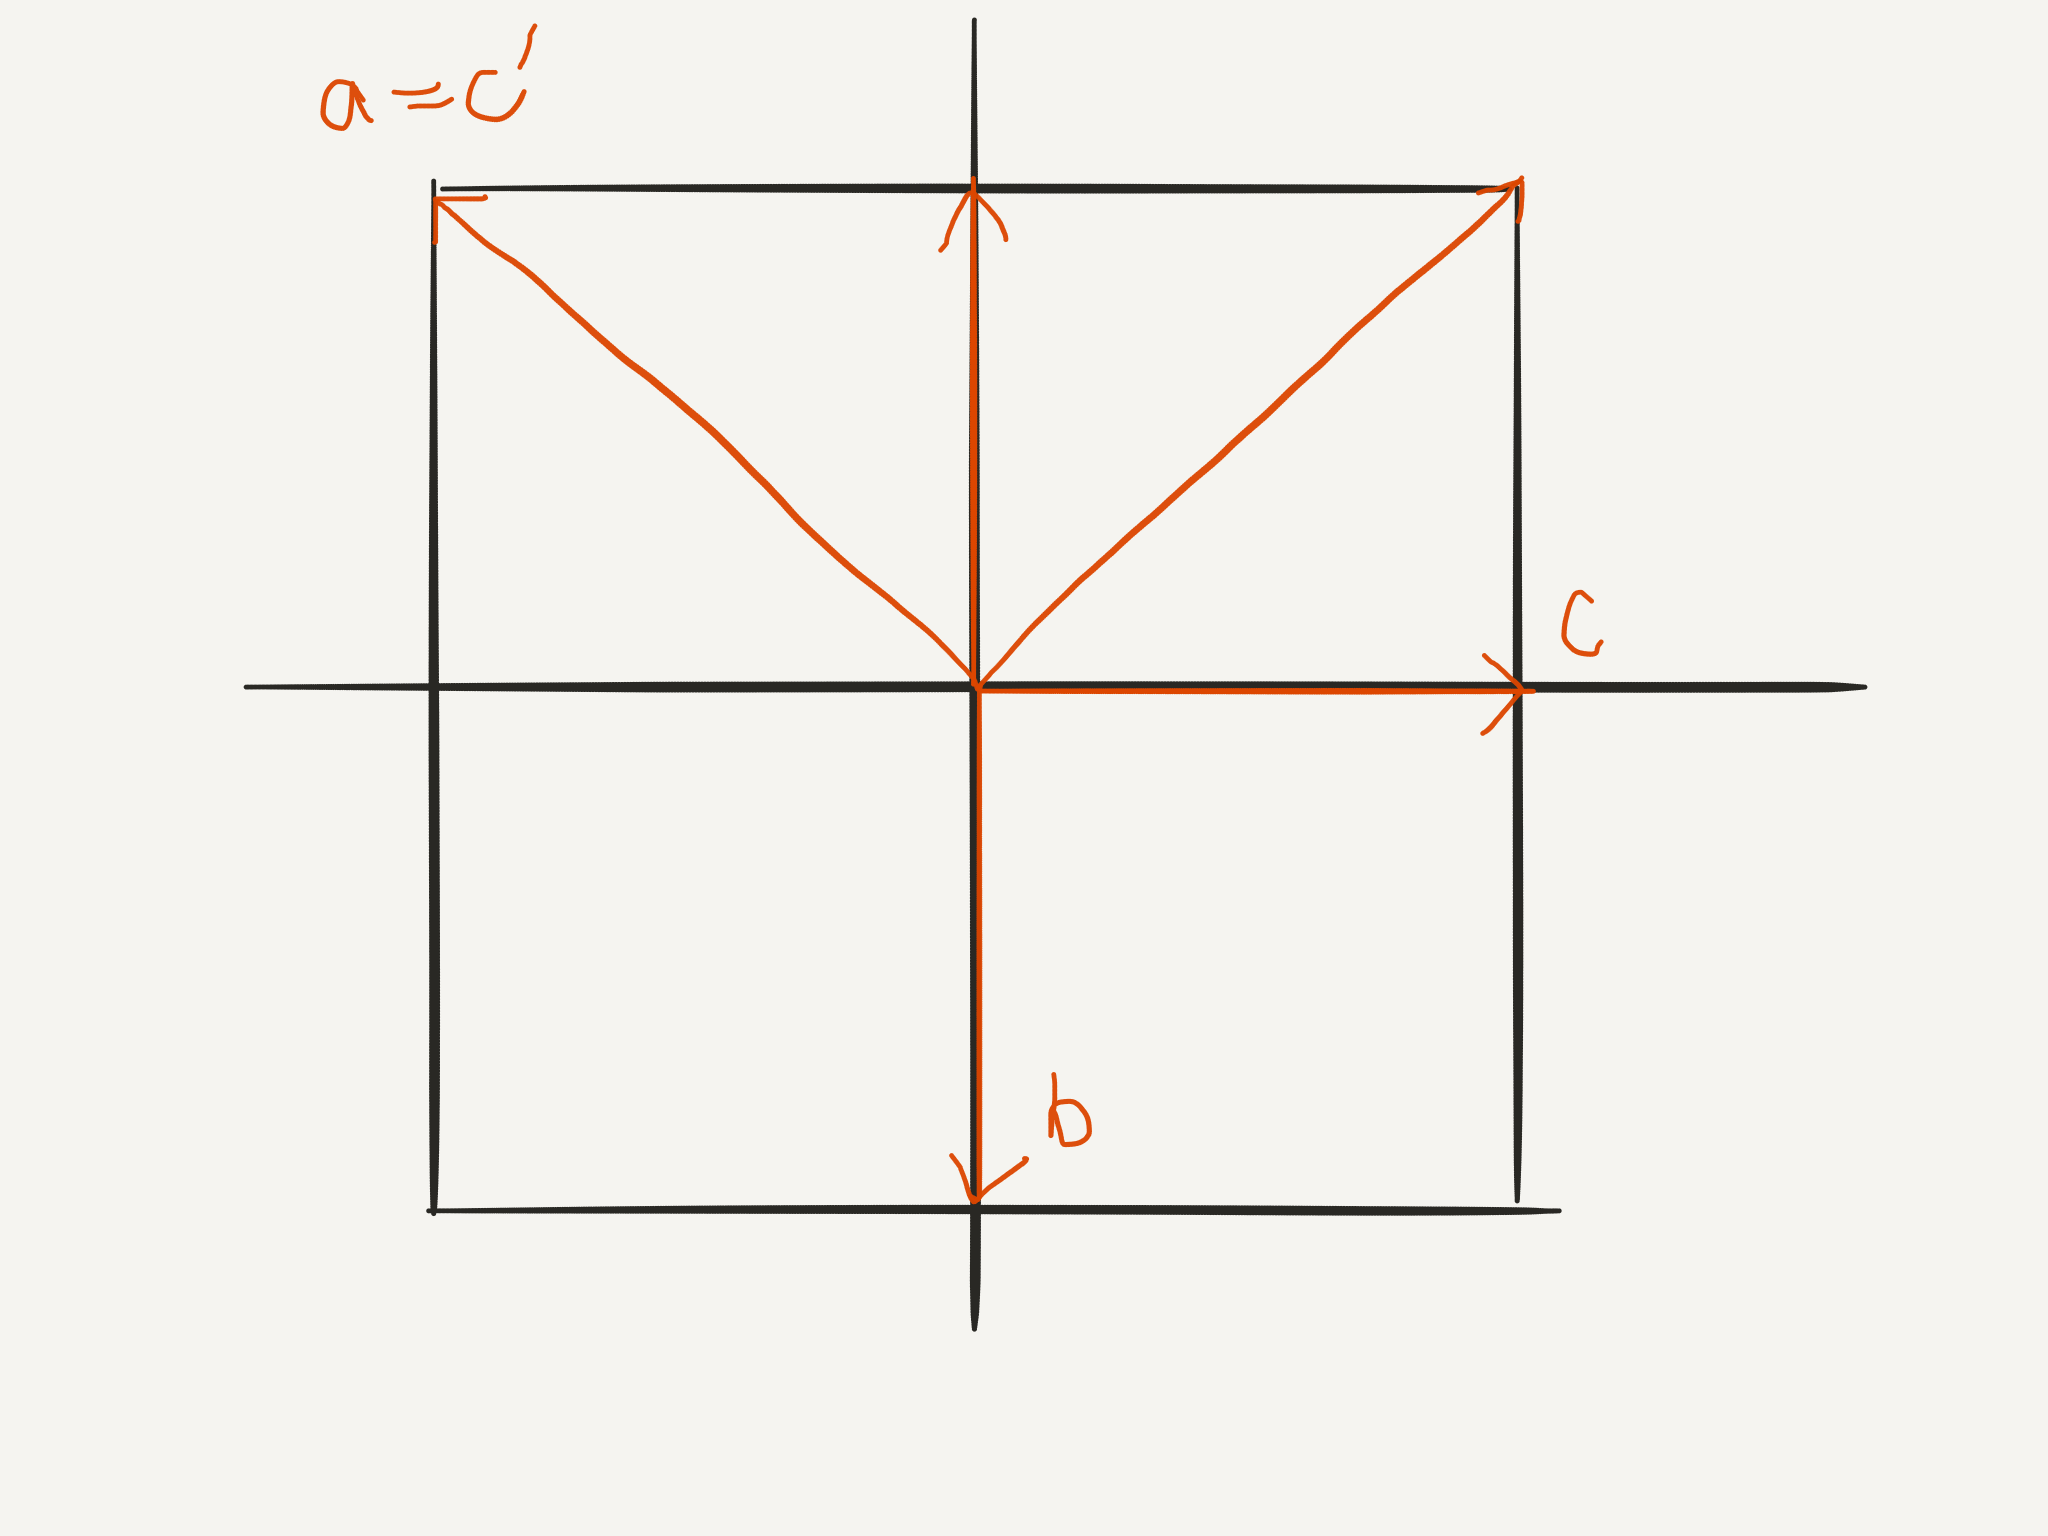
\includegraphics[scale=.2]{249-13.png}
\]
In this case we have $b,-b \in \Psi$ so $-a = r_b(c'+2c) \in \Psi$. Then $\pm a \in \Psi$, so $\Psi$ contains 
$r_a(b) = a+b$. 

For the root system G$_2$, the subset of roots with a common length in G$_2$
is a copy of A$_2$. We have already settled A$_2$, so for the case-checking with G$_2$ we may assume
that if $a$ and $b$ have the same length then each is short
and $a+b$ is long.
\end{proof}

The following consequence of Theorem \ref{pardyn} in the split case will later be generalized to incorporate
the non-split case.

\begin{lemma}
For a split reductive pair $(G,T)$, there is a natural inclusion-preserving bijection 
\begin{align*}
\{ \text{parabolics $\supset T$}\} & \Longleftrightarrow \{ \text{parabolic subsets of $\Phi(G,T)$}\} 
\end{align*}
\end{lemma}

\begin{proof}
The maps are 
\begin{align*}
P & \mapsto \Phi(P,T) \\
P_G(\lambda) = \langle T, \{U_c\}_{c \in \Psi} \rangle & \mapsfrom \Psi = \Phi_{\lambda \geq 0}
\end{align*}
The inclusion-preserving nature follows from the explicit descriptions.
\end{proof}

\begin{remark}
The preceding proof
shows that parabolic $k$-subgroups $P,P' \supset T$ we have $P \supset P'$
if and only if $\Lie(P) \supset \Lie(P')$.
 The conditions on both sides of this equivalence do not refer to $T$, so one might wonder if it is true even 
 without the assumption $P,P' \supset T$ or more generally without
 assuming $G$ contains a split maximal $k$-torus at all. 
 
 Later we'll show that for parabolic
 $k$-subgroups $P,P'$ in a connected reductive group $G$ over any field $k$, 
 $P \cap P'$ is smooth and contains a maximal $k$-torus of $G$. (Note that to prove this
 assertion it suffices to work over $\ol{k}$.) 
 Therefore, $P \subset P'$ if and only if $\Lie(P) \subset \Lie(P')$ because it is enough to 
 check over $\ol{k}$, where a choice of common maximal torus in $P$ and $P'$ becomes split.
\end{remark}

As another application, we can settle a question raised in Remark \ref{N(P)}:

\begin{lemma}\label{schemeN(P)} If $P$ is a parabolic $k$-subgroup of a connected reductive $k$-group $G$
then the scheme-theoretic normalizer $N_G(P)$ coincides with $P$.
\end{lemma}

\begin{proof}
We can assume $k = \ol{k}$.  Since equality holds on geometric points 
(Theorem \ref{Chevalley}) and $P$ is smooth and connected, 
it suffices to check equality of tangent spaces.  From the functorial meaning of $N_G(P)$, 
if $X \in {\rm{Lie}}(N_G(P))$ then ${\rm{Ad}}_G(g)(X) - X \in {\rm{Lie}}(P)$ for all $g \in G(k)$.
If $T \subset P$ is a maximal torus and ${\rm{Lie}}(N_G(P))$ is strictly
larger than ${\rm{Lie}}(P)$ then we can pick such $X \ne 0$ that is an eigenvector for $T$, say
with weight $a$.  Hence, for all $t \in T(k)$ we have $(a(t)-1)X \in {\rm{Lie}}(P)$, forcing
$a = 1$.  Thus, it suffices to show that all $T$-weights on ${\rm{Lie}}(G)/{\rm{Lie}}(P)$
are nontrivial.  But we can pick $\lambda \in {\rm{X}}_{\ast}(T)$ such that $P = P_G(\lambda)$,
so $U_G(-\lambda) \rightarrow G/P$ is an open neighborhood of the identity.  In particular,
all $T$-weights $a$ on ${\rm{Lie}}(G/P) = \mathfrak{g}/\mathfrak{p}$ satisfy
$\langle a, \lambda \rangle < 0$, so $a \ne 1$.
\end{proof}

As a final application of Theorem \ref{pardyn}, consider the expression $P = P_G(\lambda) = Z_G(\lambda) \ltimes U_G(\lambda)$
with $Z_G(\lambda)$ connected reductive (by Proposition \ref{ztorusconn} and Theorem \ref{unip2}) and $U_G(\lambda)$
a $k$-split smooth connected unipotent $k$-group. It follows that $\mathscr{R}_{u,k}(P) = U_G(\lambda)$ is $k$-split
and descends $\mathscr{R}_u(P_{\overline{k}})$, and that $L := Z_G(\lambda)$ is a ``Levi $k$-subgroup'' of $P$
in the sense that the natural map $L_{\overline{k}} \rightarrow P_{\overline{k}}/\mathscr{R}_u(P_{\overline{k}})$ is an isomorphism. 
To appreciate how remarkable it is that parabolic $k$-subgroups of connected
reductive groups always admit a Levi $k$-subgroup (usually called a ``Levi factor''), 
we note that over every algebraically closed field of positive characteristic
there exist smooth connected linear algebraic groups admitting no Levi subgroup.  This phenomenon, and a more favorable analogue
over all fields of characteristic zero, is discussed in Appendix \ref{levi}.

\section{Maximal split tori and minimal parabolic subgroups} 

\subsection{Conjugacy results and first steps of proof}

The following theorem (to be proved!) underlies the structure theory of
connected reductive groups over general fields.

\begin{theorem}\label{conj_tori_par}
Let $G$ be a connected reductive group over a field $k$. 
\begin{enumerate}
\item The maximal split $k$-tori are $G(k)$-conjugate.
\item The minimal parabolic $k$-subgroups are $G(k)$-conjugate. 
\end{enumerate}
\end{theorem}

Note that (1) is only interesting if there is a non-central split $k$-torus, and 
(2) is only interesting when there is a proper parabolic $k$-subgroup. But
we have seen in Remark \ref{partorus} 
via the dynamic description of parabolic $k$-subgroups there is a non-central split 
$k$-torus if and only if there is a proper parabolic $k$-subgroup,
so the interesting cases of (1) and (2) either both occur or both do not occur. 

\begin{remark} Warnings:
\begin{itemize}
\item Do not confuse maximal split $k$-tori with split maximal $k$-tori. 
\item In general there may not be Borel $k$-subgroups, 
so the minimal parabolic $k$-subgroups may not be solvable.
\end{itemize}
\end{remark}

\begin{exercise}
Read Appendix \ref{rootdatum}, especially Examples \ref{rootex} and \ref{root2.2} for 
comparing root data of $G$ and $\Cal{D} G$, as
well as comparing root data for $G$ versus $G/Z_G$ (including the special case $G = {\rm{GL}}_n$). 
See the October 25, 2011 Eilenberg lecture by B. Gross (at Columbia) on YouTube. 
\end{exercise}

Before we prove Theorem \ref{conj_tori_par} we record some consequences.

\begin{lemma}
If there exists a Borel $k$-subgroup $B \subset G$, then every minimal parabolic $k$-subgroup is a Borel, and all such are $G(k)$-conjugate. 
\end{lemma}

\begin{proof} By dimension reasons every parabolic $k$-subgroup contains a minimal one,
and certainly $B$ is minimal (as it is even minimal over $\ol{k}$).
Thus, by part (2) of Theorem \ref{conj_tori_par},
every parabolic $k$-subgroup of $G$ contains a $G(k)$-conjugate of $B$, so
the minimal parabolic $k$-subgroups of $G$ are precisely the $G(k)$-conjugates of $B$. In particular,
such $k$-subgroups are Borel $k$-subgroups. 
\end{proof}
	
\begin{lemma}
If $G$ is split, then every Borel $k$-subgroup contains a split maximal $k$-torus.
\end{lemma}


\begin{proof} By hypothesis $G$ contains a split maximal torus $T$. We know that we can construct Borel $k$-subgroups containing $T$ via the dynamic method: these are $P_G(\lambda)$
for a regular cocharacter $\lambda \in {\rm{X}}_{\ast}(T)$. Since Theorem \ref{conj_tori_par} tells us that all Borel $k$-subgroups are conjugate, it follows that every Borel $k$-subgroup contains a split maximal torus
(in fact a $G(k)$-conjugate of $T$). \end{proof}

\begin{example}
Later we'll see that for a non-degenerate 
finite-dimensional quadratic space $(V,q)$ and a non-degenerate finite-dimensional
hermitian space $(W,h)$
(relative to separable quadratic extensions $k'/k$), usually $\SO(q)$ and $\SU(h)$ are \emph{not} quasi-split (the minimal parabolic $k$-subgroups and maximal split
$k$-tori will be related to maximal isotropic subspaces for the bilinear form $B_q$ and sesquilinear form $B_h$
respectively). 
\end{example}

Appendix \ref{compact} shows that 
 for connected semisimple  $G$ over a local field $k$ (including $k= \R$), $G$ has no proper parabolic $k$-subgroup (which is equivalent to $G$ being $k$-anisotropic) if and only if $G(k)$ is compact. Of course if $G(k)$ is compact then $G$ is $k$-anisotropic (equivalently, $G$ contains no proper parabolic $k$-subgroup), 
 so the converse is the interesting part. 

\begin{example}
If $k$ is any field and $D$ is a finite-dimensional central division algebra over $k$
then by Exercise 1 of Homework 8 of the previous course
the connected semisimple $k$-group ${\rm{SL}}_1(D)$ of units of reduced norm 1 
in $D$ (i.e., the $k$-group scheme whose points valued in a $k$-algebra $R$ are the units with reduced norm 1 in
the Azumaya $R$-algebra $R \otimes_k D$) is
$k$-anisotropic.  

It is a deep result of Bruhat and Tits (beyond the scope of this course) that over a non-archimedean local field $k$,
up to central isogeny 
these are the {\em only} nontrivial connected semisimple $k$-groups that are $k$-anisotropic 
and absolutely simple (i.e., have no nontrivial proper normal subgroups over $\overline{k}$).
\end{example}

\subsection{Proof of part (1) of Theorem \ref{conj_tori_par}}

We will prove (1) by induction on $\dim G$. We may assume
that there are non-central split $k$-tori (as otherwise
the only maximal split $k$-torus is the maximal split $k$-subtorus
of the unique maximal central $k$-torus $Z \subset G$), 
so any {\em maximal} split $k$-torus $S \subset G$ is non-central.
In particular, there must exist a proper parabolic $k$-subgroup $P$.  
We will apply dimension induction to a Levi $k$-subgroup $L \subset P$
(e.g., $L = Z_G(\lambda)$ for $\lambda: \G_m \rightarrow G$ such that $P = P_G(\lambda)$).
To carry out such dimension induction with $L$, we require:

\begin{proposition}\label{GPprop}  For a connected reductive $k$-group $G$ and 
a parabolic $k$-subgroup $P$, the natural map $G(k) \rightarrow (G/P)(k)$
is surjective.
\end{proposition}


A natural first attempt at proving such surjectivity
is to note that for $\xi \in (G/P)(k)$, the fiber $\pi^{-1}(\xi) \subset G$ is a (right) torsor for $P$, 
so we can try to show that \emph{all} $P$-torsors are trivial (i.e. have a $k$-point)
when $P \neq G$ (the case $P=G$ being trivial in Proposition \ref{GPprop}). 
This works if $P= B$ is a Borel $k$-subgroups containing a split maximal $k$-torus $T$, since 
then $B = T \ltimes \mathscr{R}_{u,k}(B)$ is filtered by $\G_a$'s and $\G_m$'s, so
${\rm{H}}^1(k,B) = 1$. 

However, the triviality
of $P$-torsors more generally is \emph{false}, as we'll see in a moment. 
The upshot is that we {\em cannot} expect to prove Proposition \ref{GPprop}
by a purely cohomological argument. More specifically, 
the fiber of $\pi:G \rightarrow G/P$ over any $\xi \in (G/P)(k)$ is a $P$-torsor, but 
even if $G$ is split it can happen (for many $k$)  that there exist
non-trivial $P$-torsors over $k$. Hence, the absence of such torsors in the fibers of $\pi$
over $(G/P)(k)$ is remarkable.  Here is an example:

\begin{example} Let $G = {\rm{PGO}}(q) = {\rm{PGO}}_N$
for the standard split non-degenerate quadratic form
$$q = x_1 x_N + x_2 x_{N-1} + \dots$$
in $N$ variables with $N \ge 4$; this is ${\rm{SO}}_N$ for odd $N$ and ${\rm{SO}}_N/\mu_2$
for even $N$.  The 1-parameter subgroup $\lambda(t) = {\rm{diag}}(t, 1,  1, \dots, 1, t^{-1}) \bmod \mathbf{G}_m$
gives rise to a proper parabolic $k$-subgroup $P = P_G(\lambda) = L \ltimes U$
with $k$-split $U = U_G(\lambda)$ and $L = Z_G(\lambda)$.  We have $L  = {\rm{GO}}(q')$
for $q' := x_2 x_{N-1} + \dots$ a split non-degenerate quadratic form in $N-2$ variables
(check separately for odd $N$ and even $N$, using the good
behavior of torus centralizers under quotient maps in the latter case). 

For any $L$-torsor $E$ whose pushout along $L \rightarrow P$
is trivial, $E$ is trivial since there is a retraction homomorphism $P \twoheadrightarrow P/U = L$.
(Using the insensitivity of the $k$-split
property under $k_s/k$-twisting of unipotent connected linear algebraic $k$-groups, one
can even show that the sets of isomorphism classes of $L$-torsors and $P$-torsors over $k$ are in natural bijection
under such pushout.)  Thus, to exhibit a nontrivial $P$-torsor over $k$
it suffices to construct a non-trivial torsor over $k$ for $L = {\rm{GO}}_{N-2}$.

Since ${\rm{GO}}_{N-2}$ is the group scheme of conformal automorphisms of the standard split
quadratic space of rank $N-2$, the isomorphism class of an $L$-torsor over $k$ is ``the same'' as the conformal
isometry class (i.e., homothety class) of a non-degenerate quadratic space of rank $N-2 \ge 2$
over $k$.  Hence, the class of such a $k$-anisotropic quadratic space (of which there
are many examples over any global field $k$) does the job. 
\end{example}


\begin{proof}[Proof of Proposition \ref{GPprop}]
For finite $k$, all torsors for a smooth connected $k$-group are trivial by Lang's Theorem. 
Thus, the naive idea works in this case, so we may and do 
assume $k$ is infinite. Now the crucial fact is that $G(k) \subset G$ is Zariski dense! This follows from: 

\begin{proposition}\label{uniprop}
For any field $K$, a connected linear algebraic $K$-group $H$ is unirational 
(over $K$) if $K$ is perfect or $H$ is reductive. 
\end{proposition}

Recall that by definition a geometrically integral scheme $X$ 
of finite type over a field $K$ is {\em unirational} (over $K$)
when there is dominant $K$-morphism $\Omega \rightarrow X$ with $\Omega$ dense open in
an affine space over $K$.  

Proposition \ref{uniprop} is proved as the main result in Appendix \ref{unirat}, where it is shown that the hypotheses
are optimal by giving a non-unirational unipotent $H$ over any imperfect field.

Let's give some brief comments on the proof of unirationality in the reductive
case over any field (to which the general case over perfect fields is reduced, using
the split property of unipotent connected linear algebraic groups over perfect fields).
The idea for infinite $K$ is to show that $H$ is generated by its maximal 
$K$-tori (reducing unirationality to the case of tori). More precisely,  for infinite $K$ 
one uses Zariski-density considerations in Lie algebras (reminiscent of the proof of Grothendieck's
theorem on maximal tori) 
to build $K$-tori $T_1, \ldots, T_n \subset H$ such that the multiplication map of $K$-schemes
\[
T_1 \times \ldots \times T_n \rightarrow H
\]
is dominant.  A natural method is to try to find tori whose Lie algebras span the Lie algebra of $H$, 
though that does not actually work in general
(e.g., in characteristic 2 all maximal tori in ${\rm{SL}}_2$ have the {\em same} 1-dimensional Lie algebra,
namely the Lie algebra of the central $\mu_2$), forcing one to instead use dimension induction via
centralizers of semisimple elements in the Lie algebra. 

The unirationality of tori can be handled directly by 
arguing with Galois lattices: any Galois lattice occurs inside a direct product
of finitely many induced Galois lattices, so any torus
over a field $K$ is a quotient of a direct product of finitely many Weil-restricted
tori of the form ${\rm{R}}_{K'/K}(\mathbf{G}_m)$ for separable finite extensions $K'/K$.
But as a $K$-scheme such a Weil restriction is dense open inside ${\rm{R}}_{K'/K}(\mathbf{A}^1_K) =
\mathbf{A}^{[K':K]}_K$.

Returning to the proof of Proposition \ref{GPprop}, 
we'll show that $G \rightarrow G/P$ has Zariski-local sections. (This obviously implies that the induced map of rational points is surjective.) 
%We'll find a section over some dense open and
%then translate it by $k$-points of $G$ to make enough local sections to over $G/P$.
%
So we want to show that there is an open cover $\{\Omega_{\alpha}\} $ of $G/P$ such that $\pi^{-1}(\Omega_{\alpha}) \rightarrow \Omega_{\alpha}$ has sections (over $k$) for all $\alpha$. How can we do this? 

One such dense open subset of $G/P$ is provided
by the dynamic method: we know that $P =P_G(\lambda)$ for some $k$-homomorphism
$\lambda: \G_m \rightarrow G$, so 
\[
U_G(-\lambda) \times P \rightarrow G
\]
is an open immersion. Then by descent theory $U_G(-\lambda) \rightarrow G/P$ is an open immersion, so the image $\Omega \subset G/P$ has a section 
\[
\xymatrix @C=4pc{
U_G(-\lambda) \ar[d]_{\simeq} \ar@{^{(}->}[r]  & G \ar[d] \\
\Omega \ar@{^{(}->}[r] & P/G
}
\]

Clearly we have sections over $g \cdot \Omega$ for all $g \in G(k)$ (by applying $g$-translation
to the section over $\Omega$). Hence, it is enough to show that $\{g \cdot \Omega\}_{g \in G(k)}$ covers $G/P$. But $G(k) \subset G$ being Zariski dense implies that $G(k) \subset G_{\ol{k}}$ is Zariski-dense (by expressing the injectivity in terms of injectivity of the total evaluation map 
\[
k[G] \rightarrow \prod_{x \in G(k)} k
\]
and then tensoring with $\ol{k}$, using that $V \otimes_k \prod_i W_i \rightarrow \prod_i (V \otimes_k W_i)$
is injective for any vector space $V$ and collection of vector spaces $\{W_i\}$).
It then follows that $\{ g \Omega_{\ol{k}}\}$ is an open cover of $(G/P)_{\ol{k}}$ 
because (by the Nullstellensatz) such an ``open covering'' property for $\ol{k}$-schemes of finite type
may be checked on $\ol{k}$-points: if $x \in (G/P)(\ol{k})$
and $g_0 \in G(\ol{k})$ represents $x$ then the non-empty open set $\Omega_{\ol{k}} g_0^{-1}$
has non-empty open preimage in $G_{\ol{k}}$
that must contain some point $g$ in the dense subset $G(k)$, 
so $g.x \in \Omega_{\ol{k}}$ and hence $x \in g^{-1}\Omega_{\ol{k}}$.
\end{proof}

The following important consequence of Proposition \ref{GPprop} is the analogue
over general fields of the fact that a Borel subgroup over an algebraically closed
field contains a conjugate of any connected solvable closed subgroup:

\begin{lemma}\label{fixed_pt}
Let $G$ be a connected reductive group over a field $k$, and $P$ a parabolic $k$-subgroup.
Let $H \subset G$ be a connected linear algebraic $k$-subgroup that is split-solvable 
(i.e. has a composition over $k$ with successive quotients $\G_a$ or $\G_m$). 
There exists $g \in G(k)$ such that $gHg^{-1} \subset P$. 
\end{lemma}

This result will be used with $H$ a torus in our proof of Theorem \ref{conj_tori_par}(1),
and with $H$ unipotent in our proof of Theorem \ref{conj_tori_par}(2). 

\begin{proof} The connected split-solvable 
$H$ acts by left translation on the proper $k$-scheme $X=G/P$
for which $X(k) \neq \emptyset$. Then the Borel fixed point theorem, which applies for 
\emph{connected split-solvable} groups acting on proper schemes with a rational point over a field (as shown in the previous course), 
says that there is a rational fixed point $x \in X(k)$ fixed by $H$. But $X(k) = G(k)/P(k)$ by
Proposition \ref{GPprop}, and if $g \in G(k)$ represents $x$ then $g^{-1} H g \subset P$. 
\end{proof}

We have carried out the preliminaries needed
to finally give the proof of part (1) of Theorem \ref{conj_tori_par}!
 Let $S \subset G$ be a maximal split $k$-torus. We 
 all such $S$ to be $G(k)$-conjugate to each other. If one such $S$ is central then we are done
 (as for any split $k$-torus $S'$ the $k$-group generated by $S$ and $S'$
 is a quotient of $S \times S'$ by centrality of $S$, so it is a split $k$-torus containing $S$
 and thus equal to $S$ by maximality, forcing $S' \subset S$). 
 
 Now we can assume  all such $S$ are non-central.  In particular, 
there exists a \emph{proper} parabolic $k$-subgroup $P = P_G(\lambda) = L \ltimes U$ for $L = Z_G(\lambda)$ a lower-dimensional connected reductive group, and $U = U_G(\lambda)$ a connected unipotent $k$-subgroup
that is {\em split} (by Proposition \ref{uagsplit} applied
with the action of the torus $\G_m$ through $\lambda$
and the subsemigroup $A \subset {\rm{X}}(\G_m) = \Z$ consisting of positive integers). 
By Corollary \ref{fixed_pt}, every $S$ admits
a $G(k)$-conjugate contained in $P$, so 
we may limit ourselves to only study maximal $k$-split tori of $G$ contained in $P$. 

The composition
\[
S \hookrightarrow P \twoheadrightarrow P/U \simeq L
\]
realizes $S$ as a split $k$-torus of $P/U$, with $\dim(P/U) < \dim G$.  By dimension induction, the image of
$S$ in $P/U$ admits a $(P/U)(k)$-conjugate contained inside a {\em fixed choice} of maximal
split $k$-torus $S_0 \subset P/U$.  But $P(k) \rightarrow (P/U)(k)$ is surjective 
because the $k$-subgroup $L \subset P$ maps isomorphically onto $P/U$.
Identifying $S_0$ with a $k$-subtorus of $L$ in this manner,
it is enough to study maximal split $k$-tori of $G$ lying in $H_0 = S_0 \ltimes U$ for 
the split torus $S_0$ and the split connected unipotent $U$ normalized by $S_0$. 

Our general conjugacy claim for maximal split $k$-tori in arbitrary connected reductive $k$-groups
has been reduced to the same for $k$-groups of
the form $H_0 = S_0 \ltimes U_0$ where $S_0$ is a split $k$-torus
acting on a split connected unipotent linear algebraic $k$-group $U_0$. For this
we shall use induction on $\dim U_0$ to eventually reduce to the case of
a linear representation of $S_0$ on a vector space, which we will be able to treat by bare hands. 


\begin{remark}
Every $k$-torus $T \subset H_0$ is split since the composition $T \hookrightarrow H_0/U_0 = S_0$ 
has trivial kernel.  Hence, we aim to prove $H_0(k)$-conjugacy of all maximal $k$-tori in $H_0$.
\end{remark}

\begin{remark}[Warning]
If ${\rm{char}}(k) = p>0$ and  the split connected unipotent $U_0$ is commutative
and $p$-torsion then $U_0 \simeq \G_a^n$ (see Exercise G.1 in Appendix \ref{solvgp}) but $\Aut(\G_a^n)$ is much bigger than $\GL_n$ for $n > 1$. The standard example of a non-linear automorphism is 
\begin{align*}
\G_a \times \G_a & \simeq \G_a \times \G_a \\
(x,y) & \mapsto (x+y^p, y)
\end{align*}
Thus, the $\G_a$-module structure on such $U_0$ is highly non-unique in general, so finding one that is $S_0$-equivariant is not obvious. 

The situation is better in characteristic $0$:
 the endomorphism functor of $\G_a$ on the category of $\Q$-algebras is represented by $\G_a$
(as the only additive polynomials over a $\Q$-algebra are the degree-1 monomials), so the automorphism
functor of 
$\G_a^n$ on the category of $\Q$-algebras is represented by $\GL_n$.
Hence, any action on $\G_a^n$ by a group scheme in characteristic 0 is necessarily linear. 
\end{remark}

We'll argue by induction on $\dim U_0$ via $S_0$-equivariant composition series of $U_0$ over $k$ in \emph{split} connected linear algebraic $k$-subgroups of $U_0$. The point is to use such a composition series to simplify the situation, eventually reaching the case that $U_0$ is a linear representation of $S_0$.
As a first step, we record some good properties of the ``split'' condition for
connected unipotent linear algebraic groups over a general field. (Recall that over imperfect fields a split 
connected unipotent linear algebraic group can have non-split smooth connected
subgroups, such as Rosenlicht's example of a non-split form of $\G_a$ as a subgroup of
$\G_a^2$, in contrast with the analogue for tori.)

We need three facts about splitness in the connected unipotent case. 
\begin{enumerate}
\item It is inherited by quotients (\emph{not} by $k$-subgroups in general).
\item It always holds for $k$ perfect (e.g. characteristic $0$ or finite fields).
\item It is inherited by the derived group.
\end{enumerate}
For (1) and (2) see \S 20 of the notes from the first course. Assertion (3) is more subtle,
so we sketch the idea.
Recall that the derived group is generated by a bounded number of commutators; i.e., for the commutator map 
of $k$-schemes $c \colon U \times U \rightarrow \Cal{D}(U)$, there exists some 
integer $n>1$ such that  the multiplication of $n$ commutators
\[
(U \times U)^{n} \rightarrow \Cal{D}(U)
\]
is dominant. Thus, (3) follows from a geometric characterization of splitness for connected unipotent 
linear algebraic $k$-groups $U$: it is equivalent to the existence of a dominant $k$-morphism 
\[
\A_k^n - Z \rightarrow U
\]
for a generically $k$-smooth closed proper subscheme $Z \subset \A_k^n$.  
This characterization is proved in Corollary \ref{mapcrit}. (There is also a counterexample in 
Remark \ref{uniratrem}, giving a 1-dimensional $U$ in characteristic 2 demonstrating the necessity of the generic smoothness hypothesis on $Z$.) The easy direction is that if $U$ is split, then it is even an affine space 
over $k$. This is proved by successive application of the fact that any
$\G_a$-torsor (for the \'etale topology) over 
an affine space over a field is itself an affine space, due to the vanishing of 
the \'etale cohomology group ${\rm{H}}^1(\A^n, \G_a)$ (via the comparison with Zariski cohomology
for quasi-coherent coefficients, for example). 

Using (3), we have an $S_0$-equivariant composition series $\{\Cal{D}^j(U_0)\}$ with each $\Cal{D}^j(U_0)$ 
actually $k$-split. Rather generally, whenever we have an $S_0$-equivariant exact sequence 
\[
1 \rightarrow U_0' \rightarrow U_0 \rightarrow U_0'' \rightarrow 1
\]
where $U_0', U_0''$ are \emph{split} connected unipotent linear algebraic
$k$-groups, then this induces an exact sequence on $k$-points (because ${\rm{H}}^1(k, U_0') = 1$), so the associated
exact sequence of $k$-groups
\[
1 \rightarrow H_0' \rightarrow H_0 \rightarrow H_0'' \rightarrow 1
\]
(built via semi-direct products against $S_0$) 
is also exact on $k$-points. In this way, we reduce the problem of showing that all maximal (split) tori are $k$-rationally conjugate to each other for $H_0$ to the same for $H_0'$ and $H_0''$. 
By applying this with the successive quotients of the derived series $\{\Cal{D}^j(U_0)\}$ 
we thereby reduce to the case where $U_0$ is commutative, as we now may and do assume. 

In characteristic $p>0$, we can further reduce to the case when the commutative
$U_0$ is $p$-torsion by using the successive quotients of 
(split!) \emph{images} $p^j(U_0)$ of multiplication by powers of $p$. (One might
try to instead use the successive kernels $U_0[p^j]$, but this runs into numerous problems:
such kernels might not be smooth or connected, if non-smooth their underlying reduced schemes might
not be subgroup schemes when $k$ is not perfect, and even if smooth and connected
perhaps they may not be split!) In this
way, we reduce to the case when the split connected unipotent commutative $U_0$
is also $p$-torsion when ${\rm{char}}(k) = p > 0$. Hence, in all characteristics $U_0$ is a vector group.

We now must confront the problem noted earlier that if ${\rm{char}}(k) > 0$ it isn't at all
clear that the vector group $U_0$ admits a $\G_a$-module structure that is
$S_0$-equivariant (i.e., can we obtain $U_0$ from a linear representation of $S_0$
on a vector space?).  Incredibly, by studying the $S_0$-action on the huge $k$-vector subspace 
$\Hom_{k\text{-gp}}(U_0, \G_m) \subset k[U_0]$, Tits was able to realize $U_0$ inside
a linear representation of $S_0$ and then refine the description to establish
the following miraculous result proved as Theorem \ref{IV.5.2.4} in Appendix \ref{solvgp}:

\begin{theorem}There exists an $S_0$-equivariant decomposition $U_0 = U_0' \times V'$ where 
\begin{itemize}
\item $S_0$ acts trivially on $U_0'$, 
\item $V'$ is a linear representation of $S_0$ with no occurrence of the trivial weight.
\end{itemize}
\end{theorem}

Since $H_0 := S_0 \ltimes U_0 = U_0' \times (S_0 \ltimes V')$, and any torus contained in $H_0$ obviously projects trivially to the unipotent direct factor $U_0'$, every such torus is contained inside
$S_0 \ltimes V'$. Thus, by replacing $U_0$ with $V'$ we may assume that $U_0$ is a linear representation of $S_0$ with no trivial weight. Using a filtration of such a representation space built from spans of eigenlines
for $S_0$, we further reduce to the case when there is a non-trivial character
$\chi \colon S_0 \rightarrow \G_m$ such that $U_0 = \G_a(\chi)$ is $\G_a$ on which $S_0$ acts
through scaling against $\chi$. 

Let $S_0' = (\ker)_{\red}^0 \subset S_0$, the codimension-1 subtorus killed by $\chi$. 
Every subtorus of a split $k$-torus always arises as a direct factor
because every $\Z^r$-quotient of $\Z^n$ always splits off as a direct summand.  
Hence, $S_0 = S_0' \times \G_m$ with $\chi$ arising from a nontrivial character on the second
factor.  This gives 
\[
H_0 =  S_0' \times (\G_m \ltimes \G_a(\chi))
\]
where $\chi(t) = t^n$ for some $n \neq 0$. Clearly every maximal torus inside $H_0$
contains the {\em central} $k$-torus $S_0'$, so we can reduce
to the case $H_0 = \G_m \ltimes \G_a$ with action $t.x = t^n x$ for some $n \neq 0$. 
Now we're facing a very tractable-looking task!

For a maximal (split) $k$-torus $T \subset H_0$ (necessarily 1-dimensional), the composition
\[
\sigma \colon T \twoheadrightarrow H_0/\G_a = \G_m
\]
is an isomorphism since the kernel is the (scheme-theoretic) intersection of $T$ with a unipotent group. 
Using $\sigma^{-1}$ to identify $T$ with $\G_m$, the inclusion of $T$ into $H_0$ becomes an inclusion having
the special form
\[
j \colon \G_m \xrightarrow{(t, f(t))} \G_m \ltimes \G_a
\]
for some Laurent polynomial $f(t) \in k[t,1/t]$. 
What is the condition on $f$ for $j$ to be a homomorphism? It turns out to be precisely that 
\[
f(tt') = f(t') + \frac{f(t)}{(t')^n}.
\]

\begin{exercise} Inspect monomial terms in $f$ to show
that it is necessary and sufficient that $f(t) = c(t^{-n} - 1)$ for some  $c \in k$. Then 
it is easy to check that $j(\G_m)$ is the $(1,c)$-conjugate of $S_0 = \G_m \times \{0\}$. 
\end{exercise}




\subsection{Proof of part (2) of Theorem \ref{conj_tori_par}}

We'll shortly begin the proof of the second part of Theorem \ref{conj_tori_par}: for a connected reductive $k$-group $G$, all minimal parabolic $k$-subgroups $P \subset G$ are $G(k)$-conjugate to each other. The proof is again a game of conjugating the object of interest into smaller groups and then applying dimension induction,
and we will use the settled $G(k)$-conjugacy of maximal split $k$-tori as part of the argument. 

First we record an interesting consequence of this second conjugacy result:

\begin{lemma}
For any extension field $K/k$ and parabolic $k$-subgroups $P,Q \subset G$, if $P_K$ and $Q_K$ are $G(K)$-conjugate then $P$ and $Q$ are $G(k)$-conjugate. 
\end{lemma}

\begin{proof}
We know that the minimal parabolics are rationally conjugate. Therefore, by using Theorem \ref{conj_tori_par} to replace $Q$ by some $G(k)$-conjugate we can assume that $P$ and $Q$ both contain a \emph{common} (minimal) parabolic $k$-subgroup. Of course the property of containing a common parabolic 
(with reference to minimality!) is preserved after ground field extension (minimality may be
destroyed in this way). 

Under such a property,
we claim that $G(K)$-conjugacy implies $P_K = Q_K$ (and thus $P=Q$). For the purpose of proving this 
refined claim, we may assume $k = K = \ol{K}$. Correspondingly, $P$ and $Q$ contain a common Borel subgroup
$B$ (by choosing a Borel subgroup of a common parabolic subgroup). 

We have by assumption $Q = gPg^{-1} \supset B$ for some $g \in G(k)$,
and also $Q \supset gBg^{-1}$ since $P$ contains $B$. 
By conjugacy of Borel subgroups of $Q$ over the algebraically closed field $k$,
there exists some $q \in Q(k)$ such that $q(gBg^{-1})q^{-1} = B$. Therefore, $qg \in N_G(B) = B$ (!). 
Hence, $qg \in B \subset Q$, so $g \in Q$ and thus $P = g^{-1}Qg = Q$ as claimed.
\end{proof}

We now move on to the proof of $G(k)$-conjugacy of any two minimal parabolic $k$-subgroups $P,Q \subset G$. By the dynamic method, there is a $k$-homomorphism $\lambda:\G_m \rightarrow G$ such that 
\[
P = P_G(\lambda) = Z_G(\lambda) \ltimes U_G(\lambda),
\]
and we know that $U_G(\lambda) = R_{u,k}(P)$ is \emph{$k$}-split. Choose a maximal split $k$-torus 
$S \subset G$. Since $P$ is parabolic, we can find a $G(k)$-conjugate of $P$ containing $S$. Therefore, without loss of generality we can assume that $P \supset S$, so 
\[
P \supset S \ltimes R_{u,k}(P).
\]
Since $S \ltimes R_{u,k}(P)$ is connected and split-solvable, by Lemma \ref{fixed_pt} we can
 replace $Q$ with a $G(k)$-conjugate so that $Q \supset S \ltimes R_{u,k}(P)$. 

\begin{proposition}\label{min_parab}
Let $G$ be a connected reductive group over a field $k$, and let $S$ be a maximal split 
$k$-torus of $G$ contained in a parabolic $k$-subgroup $P$. Then 
\begin{enumerate}
\item $Z_G(S) \subset P$ $($so $Z_P(S) = Z_G(S)$$)$, 
\item $P$ is minimal if and only if $P = Z_G(S) \cdot R_{u,k}(P)$.
\end{enumerate}
\end{proposition}

Before giving the proof of the proposition, let's see why this finishes the proof of part (2) of Theorem \ref{conj_tori_par}. Applying Proposition \ref{min_parab} to $P$ and $Q$ that each contain $S \ltimes
R_{u,k}(P)$,
with $P$ minimal, we get 
\[
P = Z_G(S) \cdot R_{u,k}(P) \subset Q.
\]
But since $Q$ is minimal, we must have $P=Q$. 

\begin{proof}[Proof of Proposition \ref{min_parab}]
Since $S \subset P$, we can find a maximal $k$-torus $T \subset P$ containing $S$. By Theorem \ref{pardyn}, we can find $\lambda \colon \G_m \rightarrow T$ such that $P = P_G(\lambda)$. Since $S$ is a maximal split torus of $G$, it is a fortiori the maximal split torus of $T$. Therefore, $\lambda(\G_m) \subset S$ inside $T$. Then anything centralizing $S$ certainly centralizes $\lambda$, so 
\[
Z_G(S) \subset Z_G(\lambda) \subset P_G(\lambda) = P.
\]
This proves (1). 

Now onto (2). Write $U = R_{u,k} (P)$ and consider the quotient map 
\[
P \twoheadrightarrow P/U =: \ol{P}
\]
onto a connected reductive $k$-group. 
%This quotient map splits since $P = L \ltimes U$, hence is surjective on $k$-points. 
Clearly $P = Z_G(S) \cdot U $ if and only if $Z_G(S) \twoheadrightarrow \ol{P}$. But recall that torus centralizers always behave well under quotient maps: the image of the torus centralizer is the centralizer of the image torus. Applying that to the surjection $P \twoheadrightarrow \overline{P}$, 
the image of $Z_G(S) = Z_P(S)$ in $\ol{P}$  is $Z_{\ol{P}}
(\ol{S})$ for the image torus $\ol{S}$ under $S \twoheadrightarrow \ol{S} \subset \ol{P}$. But 
$S \twoheadrightarrow \overline{S}$ is an isomorphism since $S \cap U = 1$
(as $S$ is a torus and $U$ is unipotent), so for dimension reasons $\ol{S}$ is maximal as a split torus of $\ol{P}$
(as $\ol{P} \simeq Z_G(\lambda) \subset G$).  

The upshot is that $P = Z_G(S) \cdot U$ if and only if the maximal split $k$-torus $\ol{S}$ in 
$\ol{P}$ is central. This is equivalent to saying that \emph{all} split tori of 
the connected reductive $\ol{P}$ are central, which is equivalent to 
the connected reductive $\ol{P}$ having no proper parabolic $k$-subgroups. Therefore, it suffices to show that $P$ has no proper parabolic $k$-subgroups of $G$ if and only if $\ol{P}$ has no proper parabolic $k$-subgroups of itself. 

We claim that a linear algebraic $k$-subgroup $Q \subset P$ is parabolic in $G$ if and only if $Q$ is
 parabolic in $P$. This is because we can always check the property of being parabolic over 
 $\overline{k}$, where it is equivalent to containing a Borel, and by dimension
 considerations the Borel subgroups of $P_{\overline{k}}$ are the same as the Borel subgroups of 
 $G_{\overline{k}}$ contained in $P_{\overline{k}}$. 

Also, \emph{every} parabolic $k$-subgroup of $P$ contains $U := R_{u,k}(P)$
because $U_{\ol{k}} = R_{u,\ol{k}}(P_{\ol{k}})$ (the dynamic construction commutes with field extension) and the unipotent radical of a linear algebraic group over $\overline{k}$
is contained in every Borel (being connected and solvable). Hence, we have established a bijection
\[
\{\text{parabolic $k$-subgroups of $P$}\} \leftrightarrow \{\text{parabolic $k$-subgroups of $P/U$}\}
\]
that completes the proof. 
\end{proof}

\subsection{Consequences}

\begin{proposition}\label{psplit}
For $P$ a parabolic $k$-subgroup of a connected reductive $k$-group $G$, all maximal split $k$-tori of $P$ are $P(k)$-conjugate. 
\end{proposition}

\begin{proof}
Write $P = L \ltimes U$ as usual, and consider the quotient map 
\[
P \twoheadrightarrow P/U \xleftarrow{\sim} L.
\]
We saw above that any maximal split $k$-torus $S \subset P$ 
maps isomorphically onto a maximal split $k$-torus $\ol{S} \subset P/U$.
By the settled reductive case, all such $\ol{S}$'s are $(P/U)(k)$-conjugate.
Also, $P(k) \twoheadrightarrow (P/U)(k)$ because $P = L \ltimes U$. 
Therefore, we can reduce to considering those $S$ for which $\overline{S}$
is equal to a fixed $\ol{S}_0 \subset P/U$ for a fixed maximal split
$k$-torus $S_0 \subset P$. Hence, $S \subset S_0 \ltimes U$.
But rational conjugacy is already known for semidirect products of a split torus
against a split connected unipotent linear algebraic $k$-group, as we saw
in the \emph{proof} of Theorem \ref{conj_tori_par}.
\end{proof}


We want to refine some of the conclusions above. For instance, we showed that $P = Z_G(S) \cdot R_{u,k}(P)$
for a minimal parabolic $k$-subgroup $P$ of a connected reductive
$k$-group $G$, but we want to upgrade this to a semidirect product
(e.g., that is useful for calculations with rational points).

\begin{example}
We have $\GL_n = \SL_n \cdot \G_m$ with $\G_m$ embedded diagonally, but this is rarely an equality at the level of rational points: the subgroup  $\SL_n(k) \G_m(k) \subset \GL_n(k)$ consists of
the elements whose determinant is an $n$th power inside $k^{\times}$.
\end{example}

\begin{proposition}\label{prop2}
Let $G$ be a connected reductive $k$-group,
$S \subset G$ a maximal split $k$-torus, and
$P \subset G$ a minimal parabolic $k$-subgroup
such that $S \subset P$. Let $U = R_{u,k}(P)$ $($which is $k$-split$)$. 

Then $P = Z_G(S) \ltimes U$; i.e., $Z_G(S) \cap U = 1$ as $k$-group schemes.
\end{proposition}

\begin{proof}
Since $U$ is normal in $P$ and $S \subset P$, certainly $S$ normalizes $U$.  Thus, 
$Z_G(S) \cap U$ coincides with the $S$-centralizer $U^S$ in $U$ under the conjugation
action of $S$ on $U$. For general reasons $U^S$ is smooth and connected because we can express it in terms of a torus centralizer: 
\[
Z_{S \ltimes U}(S) = S \times U^S
\]
and for any torus acting on a connected linear algebraic group
we know that the centralizer is always smooth and connected. 

But $U^S$ is normal in $Z_G(S)$ because $U$ is normal in $P$ and moreover $Z_G(S) \subset P$. Thus, 
$U^S$ is a connected normal unipotent linear algebraic $k$-subgroup of $Z_G(S)$.
Since $Z_G(S)$ is connected reductive, this forces $U^S = 1$.
\end{proof}

 
\begin{example}
We claim that 
there exist connected semisimple groups $G$ with a non-trivial unipotent normal (infinitesimal) subgroup scheme.
To make sense of this assertion,
recall that by \cite[XVII, Def.\,1.1]{SGA3}, an affine $k$-group scheme of finite type is called {\em unipotent}
if over $\overline{k}$ it admits a composition series whose successive quotients are subgroup schemes
of $\G_a$. By \cite[XVII, Theorem 3.5(i)$\Leftrightarrow$(v)]{SGA3}, this is equivalent to being a $k$-subgroup scheme of the upper-triangular unipotent subgroup of $\GL_n$ for some $n > 0$.

Assume ${\rm{char}}(k) = 2$
and consider the non-degenerate
quadratic space $(V, q)$
over $k$ with $V = k^{2n+1}$
and $q  = x_0^2 + x_1x_2 + \ldots + x_{2n-1}x_{2n}$.  The associated
symmetric bilinear form $B_q$ on $V$ has defect space $V^{\perp}$ equal to the line $k e_0$
since ${\rm{char}}(k)=2$, 
with induced non-degenerate bilinear form $\overline{B}_q$ on $V/V^{\perp} \simeq k^{2n}$
that is symplectic (as ${\rm{char}}(k)=2$). 

Consider the natural map 
\[
\SO(q) = \SO_{2n+1} \rightarrow \Sp_{2n} = \Sp(V/V^{\perp}, \overline{B}_q)
\]
induced by passage to the quotient by $V^{\perp}$
(preserved by the smooth $\SO(q)$ via consideration of $k_s$-points). 
The kernel group scheme is 
\[
\begin{pmatrix} 
1 & \\
\alpha_2 & 1 \\
 \vdots &0 & \ddots \\
 \alpha_2 & 0 & \ldots & 1
\end{pmatrix}  \simeq \alpha_2^{2n}
\]
This is commutative, unipotent, and non-trivial (and non-central; e.g., it does not lie
inside any maximal torus). 
\end{example}


\begin{lemma}\label{npz}
In the setting of Proposition $\ref{prop2}$, we have $N_G(S) \cap P = Z_G(S)$. 
Moreover, for any $\lambda \in {\rm{X}}_{\ast}(S)$ such that $P = P_G(\lambda)$
we have $Z_G(S) = Z_G(\lambda)$.
\end{lemma}

\begin{remark}
The existence of $\lambda$ as above is guaranteed by Theorem \ref{pardyn} (applied
with any maximal $k$-torus $T \subset P$ containing $S$, since any $k$-rational cocharacter of $T$
must be valued in $S$ by maximality of $S$ as a $k$-split subtorus of $T$). 
The equality $N_G(S) \cap P = Z_G(S)$
 is Step 0 towards the general {\em Bruhat decomposition} asserting the bijectivity of the natural map
\[
N_G(S)(k)/Z_G(S)(k) \simeq P(k) \backslash G(k) / P(k)
\]
(namely, the Corollary asserts that only the identity coset on the left side goes
over to the identity double-coset on the right side). 
The finite group $N_G(S)(k)/Z_G(S)(k)$ is called the \emph{relative Weyl group},
and later we will relate it to the Weyl group of a ``relative root system''
associated to the $S$-action on ${\rm{Lie}}(G)$. 
\end{remark}

\begin{proof}
We know that $P = Z_G(S) \ltimes U$, so $N_G(S) \cap P = Z_G(S) \ltimes (N_G(S)\cap U)$. 
Hence, we want to prove 
\[
N_G(S) \cap U =1.
\]
What can we say about this intersection? 

Note that $N_G(S) \cap U \hookrightarrow N_G(S)/Z_G(S)$
since we know that $Z_G(S) \cap U = U^S = 1$, and the target is finite \'{e}tale because it embeds as a 
finite type $k$-subgroup of the \'etale automorphism scheme $\Aut_{S/k}$ (as discussed
in the first course). That forces the intersection $N_G(S) \cap U$ to be finite \'{e}tale. But it is also stable under $S$ (it is straightforward to check that conjugation by $S$ stabilizes $N_G(S)$), and $S$ is \emph{connected}. 

A smooth connected group can only act trivially on a finite \'{e}tale group (by contrast, $\G_m$-scaling on $\G_a$
restricts to a nontrivial action on the finite group scheme $\alpha_p$
when $p = {\rm{char}}(k) > 0$), 
so $N_G(S) \cap U$ is centralized by $S$. Thus, $N_G(S) \cap U = Z_G(S) \cap U = 1$. 

Finally, we pick $\lambda \in {\rm{X}}_{\ast}(S)$ such that $P = P_G(\lambda)$, so
$R_{u,k}(P) = U_G(\lambda)$.  Clearly $Z_G(S) \subset Z_G(\lambda)$, yet
$P = Z_G(S) \ltimes R_{u,k}(P)$ by minimality of $P$ (see Proposition \ref{prop2}), so 
the dynamic equality $P_G(\lambda) = Z_G(\lambda) \ltimes U_G(\lambda)$ forces
$Z_G(S) = Z_G(\lambda)$. 
\end{proof}

\section{Structure of reductive groups I}

\subsection{Main goals}
We explain the goals for the structure theory of connected \emph{semisimple} groups $G$ over a field $k$. \\

{\bf I}. ({\sc Relative root systems})  Let $S$ be a maximal split $k$-torus (we now know that this is unique up to 
$G(k)$-conjugacy.) We define a set 
\[
_k \Phi := \Phi(G,S) = \{ \text{non-trivial $S$-weights on $\mf{g}$}\} \subset {\rm{X}}(S) - \{0\}.
\] 
This is a root system spanning ${\rm{X}}(S)_{\Q}$ (that breaks down for reductive $G$ if there are nontrivial central split tori, but the semisimplicity of $G$ rules out that possibility). However, 
\begin{itemize}
\item the root system ${}_k \Phi$ can be non-reduced (when $S$ is not a maximal $k$-torus)
\item for $a \in {}_k \Phi$, the weight space $\mf{g}_a \subset \mf{g}$ can be huge, 
\item the $k$-anisotropic group $M := Z_G(S)/S$ is a ``black hole'' in the sense that one can't say much about its structure. (We call $\Cal{D}(M/Z_M)$ the \emph{anisotropic kernel}.)
\end{itemize}
Note that $_k \Phi = \emptyset \iff G = Z_G(S) \iff S = 1$ (because $Z_G$ is finite). Appendix \ref{compact} proves:

\begin{theorem}
For $k$ a local field $($allowing $\R$), a connected
reductive $k$-group $G$ is $k$-anisotropic if and only if $G(k)$ is compact. 
\end{theorem}

\begin{remark}
A deeper fact is that for non-archimedean $k$ and ``absolutely simple'' $G$ (i.e., 
$G$ is connected semisimple and nontrivial with $G_{\overline{k}}$ having 
no non-trivial connected proper normal subgroup), $G$ is $k$-anisotropic 
exactly for central quotients of algebraic $k$-groups of 
units with reduced norm 1 in central division algebras over $k$. The case $k= \R$ is 
exactly the classical and highly-developed story of connected compact Lie groups. 
\end{remark}

An important global counterpart to this beyond the scope of the present course is:

\begin{theorem}
For $k$ a global field, $G$ is $k$-anisotropic if and only if $G(\A_K)/G(k)$ is compact. 
\end{theorem}

\begin{remark}
Connected reductive groups over finite fields $k$ always have a Borel $k$-subgroup,
so they have non-central split $k$-tori. 
\end{remark}

\begin{example}\label{weilks} (Example of large root spaces, repeated from Example \ref{weil_rest})
For $k'/k$ a finite separable extension and $G'$ a split connected semisimple $k$'-group (e.g. $\SL_n$), and 
$T' \subset G'$ a split maximal $k'$-torus, consider $G := R_{k'/k}(G')$. The $k$-group $G$
is connected semisimple since 
\[
G_{k_s} \simeq \prod_{\sigma \colon k' \hookrightarrow k_s /k} G' \otimes_{k', \sigma} k_s
\]
is connected semisimple of dimension $[k':k]\dim(G')$, and 
likewise $R_{k'/k}(T')$ of dimension $[k':k]\dim(T')$
is a $k$-torus that is maximal in $G$.  The maximal split subtorus $S$ 
has dimension $\dim(T')$ (since the canonical $\G_m \subset {\rm{R}}_{k'/k}(\G_m)$ is an isogeny complement to the 
norm-1 subtorus of ${\rm{R}}_{k'/k}(\G_m)$ that is $k$-anisotropic); 
for example, if $T' \simeq \G_m^{n-1}$ is the diagonal of ${\rm{SL}}_n$ over $k'$
then $S(k)$ is the ``$k$-diagonal'' in $\SL_n(k')$.

Later on we will analyze this construction in more detail and show that 
the $k$-torus $S$ is maximal split in $G$
and that the restriction map
${\rm{X}}(T') \rightarrow {\rm{X}}(S)$ (which has image $[k':k]{\rm{X}}(S)$, as we can see
by computing with the $k'$-split $T'$ replaced by $\G_m$)
induces an isomorphism ${\rm{X}}(T')_{\Q} = {\rm{X}}(S)_{\Q}$.  Moreover, we will
see that $\mathfrak{g}$ is naturally identified
with the Lie algebra over $k$ (not just vector space over $k$)
underlying $\mathfrak{g}'$, under which the $k$-subspaces
corresponding to the $T'$-root lines over $k'$ are the $S$-root
spaces, so $_k \Phi$ is identified with $\Phi(G', T')$ via restriction
${\rm{X}}(T')_{\Q} \simeq {\rm{X}}(S)_{\Q}$ and all $S$-root spaces have dimension $[k':k]$.
\end{example}

\medskip
Since the preceding example is not absolutely simple (i.e., over $\overline{k}$ it has
nontrivial connected proper normal subgroups) when $k' \ne k$, the higher dimension of
its root spaces may not be so interesting.  In the next example, which is
absolutely simple, there are nonetheless 2-dimensional root spaces.

\begin{example} (Example of non-reduced root systems) Fix $k'/k$ a quadratic separable extension and 
$\{1, \sigma \} = \Gal(k'/k)$.
For $n \ge 2$ and $0 \le q \le n/2$, consider the non-degenerate hermitian form
\[
h \colon (k')^n \times (k')^n \rightarrow k'
\]
(i.e., $h(\vec{x}, \vec{y})$ is linear in $\vec{x}$ and $\sigma$-semilinear in $\vec{y}$, and 
$h(\vec{y}, \vec{x}) = \sigma h(\vec{x},\vec{y})$) given by 
\[
h(\vec{x},\vec{y}) =\vec{x}^T \begin{pmatrix}  & 1_q & \\ \epsilon 1_q \\ & & \text{diag}(c_i) \end{pmatrix}
\sigma(\vec{y}) 
\]
where $\sigma(c_i) = c_i$ (ensuring the hermitian property)
and $\sum_{i=1}^{n-2q} c_i x_i \sigma(x_i)$ has no non-trivial zeros (``anisotropic''). 

Consider the special unitary group $G = \SU(h)$;
this is a $k$-subgroup of $R_{k'/k}(\SL_n)$ and is a $k'/k$-form of ${\rm{SL}}_n$
(see Exercise 3 in HW 7 of the first course).  We will later show that this has 
$q$-dimensional maximal split $k$-torus 
\[
S = \begin{pmatrix} t \\ & t^{-1 } \\& & 1 \end{pmatrix}
\]
with diagonal $t \in \G_m^q$ and that 
\[
_k \Phi = \begin{cases} {\rm{C}}_q, & n =2q \\
{\rm{BC}}_q, & n>2q \end{cases}
\]
where BC$_q$ is the unique non-reduced irreducible root system of rank $q$.

\end{example}

{\bf II}. ({\sc Parametrization of parabolic $k$-subgroups}) The $G(k)$-conjugacy classes of parabolic $k$-subgroups are labelled by subsets $I \subset \Delta$, where $\Delta $ is a basis of $_k \Phi$. One can even write down an explicit cocharacter $\lambda_I$ such that $P_I = P_G(\lambda_I)$, 
and $P_I \subset P_J \iff I \subset J$.  In particular, $P_{\emptyset}$ 
is a minimal parabolic $k$-subgroup of $G$ (and it contains $S$). 

Moreover, we have a bijection 
\[
\{\text{min. parabolic $k$-subgroups $\supset S$}\} \leftrightarrow \{\text{pos. systems of roots $\Phi^+ \subset_k \Phi$} \}
\]
given by $P \mapsto \Phi(P,S)$. \\

{\bf III}. ({\sc Relative Weyl group}) Let $N := N_G(S)$
and $Z := Z_G(S)$, so $N/Z$ is a finite constant $k$-group since it
is a finite type subgroup of the constant automorphism scheme
${\rm{Aut}}_{S/k} = \GL({\rm{X}}(S))_k$
(see Exercises 3 and 4 of Homework 6 of
the first course). 

We will see that the finite {\em relative Weyl group} $_kW := N(k)/Z(k) \subset {\rm{Aut}}_k(S)$
coincides with  $(N/Z)(k)$
(which is remarkable because it doesn't follow from cohomological reasons;
typically ${\rm{H}}^1(k, Z) \ne 1$) and that 
\[
_k W = W({}_k \Phi) := \langle r_a \rangle_{a \in \Delta}
\]
inside $\GL({\rm{X}}(S))$.  By design each reflection $r_a$
on ${\rm{X}}(S)_{\Q}$ will arise from $N(k)$, but it is not evident
that every element of $_k W$ arises from $W({}_k\Phi)$. 

{\bf IV}. ({\sc Bruhat decomposition}) The natural map 
\[
\frac{N_G(S)(k)}{Z_G(S)(k)} \rightarrow P_{\emptyset}(k) \backslash G(k)/P_{\emptyset}(k)
\]
is bijective; i.e., 
\[
G(k) = \coprod_{w \in W({}_k \Phi)} P_{\emptyset}(k) n_w P_{\emptyset}(k)
\]
where $n_w \in N(k)$ is a representative for $w$.
Moreover, the locally closed subsets $P_{\emptyset}n_w P_{\emptyset}$
(orbits for $P_{\emptyset} \times P_{\emptyset}$ acting on $G$ via $(p, p').g = pg{p'}^{-1}$)
are pairwise disjoint, with $$(P_{\emptyset}n_w P_{\emptyset})(k) =
P_{\emptyset}(k)n_w P_{\emptyset}(k).$$  For split $G$ these locally closed sets cover $G$
and in fact constitute a stratification
(with closure relations among the strata given by the Bruhat order on the Weyl group). But 
in general we only get a covering at the level of $k$-points, so the Bruhat decomposition
has only group-theoretic rather than geometric meaning beyond the split case. \\

{\bf V}. ({\sc Tits classification}) The possibilities for $G$ up to $k$-isomorphism
will be determined by the following data (and some relations among them which we omit here): 
\begin{itemize}
\item the anisotropic kernel $\Cal{D}(M/Z_M)$ for $M := Z_G(S)/S$ (anisotropic with trivial center,
by design); 
\item $G_{k_s}$ (equivalent to a \emph{root datum}); 
\item a continuous $\Gal(k_s/k)$-action on the Dynkin diagram $\Dyn(G_{k_s})$. 
\end{itemize}
In the split case the anisotropic kernel is trivial (as holds even in the quasi-split case, since
a Levi factor $Z_G(S)$ of a minimal parabolic $k$-subgroup is obviously a torus when the minimal 
parabolic is a Borel), and the Galois action on the diagram is trivial in the split case. 

The merit of this approach is that it enables one to sometimes prove that 
certain constructions based on linear algebra structures (quadratic forms, hermitian forms,
central simple algebras, etc.) exhaust all possibilities for a given root datum
over $k_s$.  The most important case
is when $G$ is absolutely simple,
and a precise understanding of ${\rm{Aut}}_{k_s}(G_{k_s})$ is essential to
making exhaustive lists of possibilities.  

To illustrate, for $n \ge 2$ and $G_{k_s}$ of type $B_n$
with trivial center, the absence of nontrivial diagram automorphisms will
underlie the proof that the possibilities are exactly $\SO(q)$ for non-degenerate $(V,q)$ of dimension $n$, with $\SO(q) \simeq \SO(q')$ if and only if $(V,q)$ is conformally equivalent to $(V', q')$. 
On the other hand, for type $D_n$ (informally, twisted forms of SO$_{2n}$) with $n \geq 3$, the possibilities are more complicated because the Dynkin diagram admits a nontrivial diagram automorphism. 

\medskip

The starting point for the Tits classification
is the ``Existence/Isomorphism Theorem''. A crude formulation of this
remarkable  theorem is that there is a bijection 
\[
\left\{ \text{split connected 
reductive $k$-groups} \right\}/\simeq \,\,\,\leftrightarrow \{\text{root data}\}/\simeq
\]
along with a description of ${\rm{Aut}}_k(G)$ in terms of $(G/Z_G)(k)$ and diagram automorphisms 
(upon fixing a split maximal $k$-torus). 
In particular, for any connected reductive group $G$ over $k$ 
there exists a (unique) split $k$-descent of $G_{k_s}$; this is really amazing. 

The upshot is that if we can understand the split groups \emph{and} their automorphisms, then 
we can hope to describe their Galois twists and thereby find all possibilities. This becomes 
a nontrivial problem in Galois cohomology, guided by the Galois action
on the diagram and knowledge of the relationship
between relative and absolute roots
(i.e., the root systems for $G$ and $G_{k_s}$).

\begin{remark}
The book \cite{springer} proves the Existence and Isomorphism Theorems by a
method with heavy computations 
that works only over algebraically closed fields. An alternative proof of the Isomorphism
Theorem (determining a split group by its root datum, up to isomorphism) due to Steinberg 
\cite{steinberg}
works over any field, or one can use descent theory to deduce the Isomorphism Theorem
over general fields from the case of algebraically closed fields (see the proof of 
\cite[Thm.\,A.4.6]{pred}).

But all proofs of the Existence Theorem are very hard (especially to handle the exceptional groups
in all characteristics, which is the crux of the problem).  In \cite[App.\,D]{luminy}, 
the Existence Theorem is proved over $\CC$ by an analytic method (building on results
for Lie algebras in characteristic 0 and on the theory of compact Lie groups), and in
\cite[\S6.3]{luminy} this is used to deduce a version of the Existence Theorem
over $\Z$ following the method of Demazure in \cite[Exp.\,XXV]{SGA3} (based on birational group
laws over Dedekind domains), from which the result follows
over general fields via scalar extension. This Existence Theorem over $\Z$ is
one the main results in \cite{SGA3}.  The method is very abstract but also rather clean
(when based on the dynamic method over rings, as in \cite{luminy}).

There are a variety of alternative approaches over fields due to
Steinberg, Chevalley, Lusztig, and others, often working directly
with $\Z$-structures on Lie algebras.  But ultimately 
the Bruhat--Tits structure theory for reductive groups over non-archimedean local fields
rests on a robust theory of reductive group schemes over discrete valuation rings
(possibly of mixed characteristic), and to work with such integral models
the framework of \cite{SGA3} is essential. 
\end{remark}


\subsection{Central isogeny decomposition for semisimple groups}
Root systems will turn out to classify split connected semisimple groups ``up to central $k$-isogeny''. The notion of ``central quotient'' for general connected
linear algebraic groups is not stable under composition
(consider any nilpotent connected nontrivial linear algebraic group
that is non-commutative, such as any smooth connected unipotent
group).  We will soon see that in characteristic $p>0$
even the notion of central isogeny is not  preserved
under composition, but let's first prove that everything works well
in the reductive case for all characteristics:

\begin{proposition}\label{zgmprop}
For central quotient maps 
\[
G'' \xrightarrow{f'} G' \xrightarrow{f} G
\]
between connected reductive $k$-groups, the composite map $f \circ f' \colon G'' \twoheadrightarrow G$ has central kernel. Also, if $M \subset Z_G$ is a closed $k$-subgroup then 
\[
Z_G/M \hookrightarrow Z_{G/M} 
\]
\end{proposition}

\begin{proof}
The first assertion is easily deduced from the second (as the second essentially says that under a central quotient
the center does not become ``larger than expected''). So we focus on the second assertion,
and we can assume $k = \ol{k}$ since the formation of the scheme-theoretic center 
of a linear algebraic group commutes with any extension of the ground field. In Corollary \ref{ztori}
there is a description of the center in the connected reductive case over
an algebraically closed field:
\[
Z_G = \bigcap_{T \subset G} T
\]
where $T$ varies through the set of maximal tori of $G$.  

(This description of $Z_G$ uses crucially that $G$ is reductive! The main content is that all points of the intersection,
valued in any $k$-algebra $A$, centralize the $A$-scheme $G_A$.  That intersection scheme centralizes
each $T$, so it suffices to show that maximal tori generate $G$ in the sense of
linear algebraic groups. Consider the closed linear algebraic
subgroup $N$ generated by all maximal tori. This is clearly normal, so $G/N$ is connected reductive
but contains no nontrivial tori by design, so $G/N$ is unipotent. Reductivity then forces
$G/N = 1$, which is to say $N = G$ as desired.)

 But for $M \subset Z_G$ we have a bijection between the sets of maximal tori
 \[
 \{ T \subset G \} \leftrightarrow \{\ol{T} \subset G/M\}
 \]
 via 
 \begin{align*}
 T & \mapsto T/M \\
 \pi^{-1}(\ol{T}) & \mapsfrom \ol{T}
 \end{align*}
 for the quotient map $\pi \colon G \rightarrow G/M$.  Thus, for formula for $Z_{G/M}$ in terms of intersecting
 such $\overline{T}$'s yields that the inclusion $Z_G/M \subset Z_{G/M}$ is an equality. 
\end{proof}

\begin{remark}
The preceding proof shows that what really matters about reductivity is that it
ensures generation by tori (over algebraically closed fields).  Hence, if we seek
an example beyond the reductive case for which
the formation of the center ``grows'' under a central quotient map
we are led to search among connected unipotent linear algebraic groups.

Consider the connected unipotent Heisenberg group 
\[
G = U_3 = \left\{ \begin{pmatrix} 1 & x & y \\ & 1 & z \\ & & 1 \end{pmatrix} \right\} \subset \GL_3
\]
over any field $k$ of characteristic $p>0$. 
Note that $Z_G$ is the copy of $\G_a$ in the upper right corner, the quotient by
which is the direct product of the two $\G_a$'s coming from the other matrix 
entries, so we have a short exact sequence
\[
1 \rightarrow \G_a \rightarrow G \rightarrow \G_a \times \G_a \rightarrow 1
\]
This recovers our earlier observation (valid in any characteristic) with nilpotent connected
linear algebraic groups
that the second statement in Proposition \ref{zgmprop}
can fail for non-reductive groups. 

For a counterexample to the second assertion in Proposition \ref{zgmprop}
using central \emph{isogenies} among {\em connected}
linear algebraic groups in characteristic $p>0$, consider the commutative diagram
\[
\xymatrix{
1 \ar[r] &  \G_a \ar[r] &  G \ar[r] &  \G_a \times \G_a \ar[r] &  1 \\
1 \ar[r] & \alpha_p \ar[r] \ar@{^{(}->}[u] & \ker F_{G/k} \ar[r] \ar@{^{(}->}[u] & \alpha_p \times \alpha_p \ar[r] \ar@{^{(}->}[u]  & 1
}
\]
in which the bottom row is the induced diagram among Frobenius kernels of the corresponding groups in the top
row. The bottom row is left exact a priori, and by counting orders of finite $k$-group schemes
 it is short exact because by inspection $\ker F_{G/k}$ has order $p^3$ for $G = U_3$
 (or more generally the infinitesimal Frobenius kernel of a smooth 
 $k$-group of dimension $d$ has order $p^d$
since the relative Frobenius map for a smooth $k$-scheme
 of pure dimension $d$ is finite flat with constant degree $p^d$, as we verify via an \'etale-local
 calculation to reduce to the case of an affine space).
 
 The key feature to prove is the centrality of the $k$-subgroup scheme 
\[
\alpha_p \times \alpha_p = (\ker F_{G/k})/\alpha_p \subset G/\alpha_p.
\]
Once this is known, the isogeny $F_{G/k} \colon G \rightarrow G^{(p)}$
with visibly {\em non-central} kernel will be expressed as a composition of central
isogenies $G \rightarrow G/\alpha_p \rightarrow G/\ker F_{G/k} = G^{(p)}$.

To justify the centrality claim made above, observe that for any $k$-algebra $A$ and $A$-valued point 
\[
h = \begin{pmatrix} 1 & u & * \\ & 1 & v \\ & & 1 \end{pmatrix} \in (\ker F_{G/k})(A) 
\]
with $u, v \in A$ satisfying $u^p = v^p = 0$, 
and for any 
\[ g =  \begin{pmatrix} 1 & x & y \\ & 1 & z \\ & & 1 \end{pmatrix}  \in G(A) 
\]
we have
\[
hgh^{-1} = g \cdot \begin{pmatrix} 1 & 0 & zu-xv \\ & 1 & 0 \\ & & 1 \end{pmatrix} \in \alpha_p(A) \subset
Z_G(A),
\]
so consideration with fppf group sheaves
shows that the $k$-subgroup scheme $\alpha_p \times \alpha_p \subset G/\alpha_p$ is indeed central. 
\end{remark}


\textbf{Discussion of semisimplicity.} Recall that for $\CC$-linear representations of a finite group, we have a decomposition 
\[
V = \bigoplus V_i^{e_i}
\]
for pairwise non-isomorphic \emph{irreducible} $V_i$ (and $e_i>0$), but only the \emph{isotypic subrepresentations} $W_i = V_1^{e_i} \subset V$ and their associated multiplicities $e_i$
are intrinsic; there is no intrinsic choice of $V_i$ as a subrepresentation
of $V$ when $e_i >1$. 

Similarly, for abelian varieties $A$ over an arbitrary field $k$ we know from the graduate course on abelian varieties
that  there is a $k$-isogeny (``Poincar\'e complete reducibility'' over $k$)
\[
A \sim \prod A_i^{e_i}
\]
for pairwise non-isogenous $k$-simple $A_i$ (with $e_i>0$), but only the isotypic abelian subvarieties $B_i  = 
{\rm{im}}(A_i^{e_i} \rightarrow A)$ and their associated multiplicities $e_i>0$ 
are intrinsic; there is no intrinsic choice of a $k$-isogenous quotient of $A_i$ inside $A$ when $e_i>1$. 

In these cases, for $e>1$ we have $\GL_{e_i}(\CC)$ acts on $V_i^{e_i}$ 
creating many interactions among the factors $V_i$ when $e_i > 1$,
and likewise $\GL_{e_i}(\Z) $ acts on $A_i^{e_i}$ creating many interactions among the factors
$A_i$ when $e_i>1$.  In particular, 
there are many inclusions $V_i \hookrightarrow V_i \times V_i$ 
of representation spaces and $A_i \hookrightarrow A_i \times A_i$
of abelian varieties that are not the images of factor inclusions (e.g., the diagonal homomorphism in each
case). But for \emph{non-commutative} $G$ there are no ``obvious'' automorphisms of $G \times G$ beyond swapping factors, and likewise no evident {\em normal} subgroups other than $G \times 1$ and $1 \times G$. 

\begin{example}
The diagonal $\Delta_G \subset G \times G$ is \emph{not} normal in $G \times G$ 
whenever $G$ is not commutative! (Hint: Consider conjugation against $1 \times g$ non-central $g$.) 
\end{example}

In contrast with the preceding examples, over any field $k$ connected semisimple $k$-groups admit a canonical 
central isogeny decomposition.  Let's first illustrate the result:

\begin{example}
For $G = \SL_n \times^{\mu_n} \SL_n$ or $\SO_{10} \times^{\mu_2} \Sp_6$
(gluing factors along the evident  anti-diagonal central inclusions of $\mu_n$ and $\mu_2$ respectively), 
the \emph{only} non-trivial proper normal connected linear algebraic $k$-subgroups 
of $G$ are the evident  ``factors''. 
\end{example}

The ``central isogeny decomposition'' for connected semisimple $k$-groups will be
proved later via Galois descent from the split case
over $k_s$, and it goes as follows:

\begin{theorem}\label{ss_decomp}
Let $G$ be a connected semisimple $k$-group $G$,
and $\{G_i\}$ its set of minimal non-trivial smooth connected normal 
$k$-subgroups $($all semisimple by normality, since for any smooth connected
normal $k$-subgroup $N \subset G$ the solvable radical of $N_{\overline{k}}$ 
 is stable under all $G(\overline{k})$-conjugations and hence
is contained in $\Cal{R}_u(G_{\overline{k}}) = 1$).  The following hold: 
\begin{enumerate}
\item the set $\{G_i\}$ is finite and these pairwise commute, with 
the multiplication homomorphism $\prod G_i \rightarrow G$ a central $k$-isogeny; 
\item each $G_i$ is $k$-simple;
\item the smooth connected normal $k$-subgroups of $G$ are exactly 
\[
N_J = \langle G_i \rangle_{i \in J}
\]
for subsets $J \subset I$. Moreover,
$N_J \subset N_{J'}$ if and only if $J \subset J'$
(so $G_i \subset N_J$ if and only if $i \in J$). 
\end{enumerate}
\end{theorem}

We call the $k$-subgroups $G_i$ the ``$k$-simple factors'' of $G$. The precise formulation of the full result in the \emph{split} case makes it possible to prove the general result because we can use Galois descent to pull everything down from the split case applied to $G_{k_s}$.  (Note that since normality is not transitive in non-commutative groups, it is not a tautology that each $G_i$ is $k$-simple!)  


To prove the theorem we will begin by settling  the split case via input
from the theory of root systems, 
such as an ``irreducible decomposition'' theorem for root systems.  So now we digress to
review some more facts concerning root systems.

\section{Root systems}
\subsection{Decompositions of root systems}
\begin{definition}
For root systems $(V, \Phi)$ and $(V', \Phi')$, their 
{\em direct sum} is $(V \oplus V', \Phi \coprod \Phi')$. We say that a root system $(W, \Psi)$ is \emph{reducible} if it is isomorphic to such a direct sum with $V, V' \neq 0$, and $(W, \Psi)$ is \emph{irreducible} if it's not 
$(0, \emptyset)$ and is not reducible. 
\end{definition}

\begin{example}
For a central isogeny 
\[
f:G' \times G'' \twoheadrightarrow G
\]
of split connected semisimple $k$-groups, with corresponding $k$-isogeny of split maximal $k$-tori
\[
T' \times T'' \twoheadrightarrow T
\]
(so $f^{-1}(T) = T' \times T''$ since $\ker f$ is central), 
we have $\Phi(G, T) = \Phi(G' \times G', T' \times T'')$ inside ${\rm{X}}(T)_{\Q} = {\rm{X}}(T')_{\Q} \oplus {\rm{X}}(T'')_{\Q}$
by the known invariance of the formation
of root systems with respect to central quotients.  

Clearly 
$\Phi(G' \times G'', T' \times T'') =  \Phi(G', T') \coprod \Phi(G'', T'')$, so 
we conclude that the root system $\Phi(G, T)$ is the direct product
of the root systems $\Phi(G', T')$ and $\Phi(G'', T'')$
via the equality ${\rm{X}}(T)_{\Q} = {\rm{X}}(T')_{\Q} \oplus {\rm{X}}(T'')_{\Q}$.  
(We use the standard abuse of notation that
$\Phi(G, T)$ may denote the ordered pair $({\rm{X}}(T)_{\Q}, \Phi(G, T))$ without warning.) 
\end{example}

\begin{example}
We will prove later that for a \emph{split} semisimple pair $(G,T)$, the following conditions
are equivalent:  $G$ is $k$-simple, $G_{\ol{k}}$ is $\ol{k}$-simple,  and $\Phi(G,T)$ is irreducible. 
Thus, the irreducibility of a root system is a combinatorial replacement for simplicity (in the sense
of smooth connected normal subgroups) for split connected semisimple groups.
\end{example}

Now it is time to record some facts
concerning the decomposition of root systems.  These are
all proved in \cite[VI, \S1.2]{bourbaki} (largely relying on \cite[IV, V]{bourbaki}, 
where the main work of the proofs is often found). 

\begin{proposition} Every root system $(V, \Phi)$ is uniquely a direct sum of irreducible root systems
$(V_i, \Phi_i)$.
Here, ``uniqueness'' means that the subspaces $V_i \subset V$
(and so subsets $\Phi_i = V_i \cap \Phi$)are uniquely determined.
\end{proposition}

This is much stronger than the uniqueness aspect of irreducible decomposition for characteristic-0 representations of a finite group, or of the isogeny decomposition for an abelian variety, insofar as even in the presence
of multiplicities the actual subspaces $V_i \subset V$ that arise are uniquely determined.

\begin{proposition}\label{abs_irr_root}
For irreducible $(V, \Phi)$, the action of the Weyl group $W(\Phi)$ on $V$ is absolutely irreducible. 
\end{proposition}

\subsection{Euclidean structure on root systems} The absolute irreducibility of the $W(\Phi)$-action for irreducible $(V, \Phi)$
explains the role of Euclidean geometry in the study of root systems over $\R$
(even though there is no axiom concerning a preferred inner product in the definition
of a root system or of irreducibility of root systems).  To explain this, first note that 
since $W(\Phi)$ is a finite group, by averaging we obtain a 
$W(\Phi)$-invariant positive-definite symmetric bilinear form $V \times V \rightarrow \Q$
(or equivalently a $W(\Phi)$-invariant positive-definite quadratic form $q: V \rightarrow \Q$).
Such a bilinear form is non-degenerate, and so it corresponds to a $W(\Phi)$-equivariant
isomorphism $V \simeq V^{\ast}$. Hence, by Schur's Lemma (due to the absolute irreducibility!), 
such an equivariant isomorphism is \emph{unique up to $\Q^{\times}$-scaling}.

Thus, for irreducible 
root systems $(V, \Phi)$ there is a unique homothety class of non-degenerate $W(\Phi)$-invariant
bilinear forms on $V$, so it is well-posed to speak of {\em ratios} of (squared) root-lengths
$q(a)/q(b)$ for $a, b \in \Phi$ and any $W(\Phi)$-invariant nonzero 
(necessarily definite) quadratic form $q: V \rightarrow \Q$.
Irreducible root systems that are {\em reduced}
have at most two root lengths (see \cite[VI, \S1.4, Prop.\,12]{bourbaki}). Hence, 
for reduced and irreducible root systems with at least two (and hence exactly two) root lengths
it is always well-posed to speak of a root being ``long'' or ''short''.   

Working over $\R$ (so positive elements have square roots), we can uniquely normalize a $W(\Phi)$-invariant
nonzero $Q: V_{\R} \rightarrow \R$ by the requirement that the shortest root-length is 1.
(This involves replacing an initial choice of $q$ by $q(a_0)^{-1/2} \cdot q$ for $a_0 \in \Phi$
with shortest $q$-length.) Consequently, any root system admits a {\em canonical}
Euclidean structure on its realification.  This explains why it is meaningful to draw pictures
of irreducible rank-2 root systems with specified Euclidean structure, and more generally to express
the study of irreducible root systems in terms of the Euclidean language of reflection groups,
even though there is {\em no Euclidean structure} specified in the initial definition of a root system
as in \cite{bourbaki}. 
This makes contact with other references that use Euclidean structure right
from the beginning of the study of root systems. 
Scaling the inner product has no effect on the angle between two roots, so that notion is the same regardless
of the choice of $W(\Phi)$-invariant $q$ above.


\begin{remark}
For an {\em arbitrary} (not necessarily irreducible) root system $(V, \Phi)$ there
is a ``canonical'' $W(\Phi)$-invariant positive-definite bilinear form
$B_{\Phi}: V \times V \rightarrow \Q$, given by 
$$B_{\Phi}(v, v') = \sum_{a \in \Phi} \langle v, a^{\vee} \rangle \cdot \langle v', a^{\vee}\rangle$$
where $\langle v, \ell \rangle := \ell(v)$ for $\ell \in V^{\ast}$.  Indeed, $B_{\Phi}$ is visibly
bilinear, and it is $W(\Phi)$-invariant since the effect of a reflection $r_b$ on a coroot $a^{\vee}$
is to bring it to the coroot $r_b(a)^{\vee}$; i.e., such reflections applied to $V$ have the effect
on $B_{\Phi}$ of permuting the terms in the defining sum. 

The positive-semidefiniteness of $B_{\Phi}$ is clear, and positive-definiteness holds
because the coroots span $V^{\ast}$. 

\end{remark}


To summarize, we have just seen that if a root system $(V, \Phi)$ is irreducible then the $W(\Phi)$-action on $V$ is absolutely irreducible over $\Q$, so the $W(\Phi)$-invariant symmetric isomorphism $V \simeq V^*$ is unique up to $\Q^{\times}$-scaling, and the corresponding symmetric bilinear form form $(-, -) \colon V \times V \rightarrow \Q$ is unique up to $\Q_{>0}$-scaling as a \emph{positive}-definite form. 

What about a root system which is not irreducible? In general, if $(V_i, \Phi_i)$ are the irreducible components of $(V, \Phi)$ then via the decomposition 
\[
V = \bigoplus V_i
\]
we have a decomposition of Weyl groups 
\[
W(\Phi) = \prod W(\Phi_i) .
\]
(To see this recall that from the very construction of a direct sum of roots systems, a reflection corresponding to a root in $\Phi_i$ has no effect on the $\Phi_j$ for $j \neq i$. Thus we see explicitly that the Weyl group decomposes.) Therefore, if $B \colon V \times V \rightarrow \Q$ is a non-degenerate symmetric bilinear form invariant under $W(\Phi)$ then the induced isomorphism $V \simeq V^*$ of $W(\Phi) = \prod W(\Phi_i)$-representations must carry $V_i$ to $V_i^*$ (by looking at the $W(\Phi_i)$-isotypic decompositions). So necessarily $V_i$ is $B$-orthogonal to $V_j$ for $j \neq i$ and $B$ is the orthogonal sum of the $W(\Phi_i)$-invariant 
symmetric non-degenerate forms $B_i \colon V_i \times V_i \rightarrow \Q$. 


\begin{lemma}\label{coroot}
If we fix such $B \colon V \times V \rightarrow \Q$ (positive-definite) then under the induced isomorphism $V \simeq V^*$, for each root $a \in \Phi$ the coroot $a^{\vee} \in \Phi^{\vee} \subset V^*$ corresponds to 
\[
a' := \frac{2a}{B(a,a)} = \frac{2a}{|\!|a|\!|^2_B}.
\]
\end{lemma}

\begin{remark}
This formula ``explains'' why $a \mapsto a^{\vee}$ is usually not additive. 
\end{remark}

\begin{proof}
Without loss of generality, we work in $V_{\R}$. By $W(\Phi)$-invariance, the action of $W(\Phi)$ is \emph{orthogonal}. (We originally defined a reflection to be an involution that is the identity on a hyperplane and negation on the quotient. Since we now have a Euclidean structure on which $W(\Phi)$ acts orthogonally, 
the reflections in $W(\Phi)$ are ``orthogonal reflections'' in the usual sense.) 

 For $a \in \Phi$, we have by definition
\begin{equation}\label{refl1}
r_a(x) = x - \langle x, a^{\vee} \rangle a
\end{equation}
for $a^{\vee} \in V_{\R}^{\ast}$.
On the other hand, we have the classical formula for reflection: if $u \in V_{\R}$ is a unit vector orthogonal to 
the hyperplane $\ker (a_{\R}^{\vee})$ of $r_a$-fixed points then 
\begin{equation}\label{refl2}
r_a(x)  = x - 2 (x\cdot u) u.
\end{equation}
From this we see that $u \in \R^{\times} \cdot a$ (comparing \eqref{refl1} and \eqref{refl2} for 
$x$ chosen generically so that $\langle x, a^{\vee} \rangle, x \cdot u \ne 0$). 
Hence, $u = \pm a/|\!|a|\!|$, and comparing the formulas \eqref{refl1} and \eqref{refl2} 
 again gives 
\[
\langle x, a^{\vee} \rangle a = \frac{x \cdot 2a}{|\!|a|\!|^2} a.
\]
Thus, the linear functional $a^{\vee} \in V^{\ast}_{\R}$ is given by dot product against
$2a/|\!|a|\!|^2$.
\end{proof}

\begin{example}
For the root system A$_2$ corresponding to $\SL_3$ we have $c^{\vee} = 2c$
when the Euclidean structure is normalized to make all roots unit vectors. 
\[
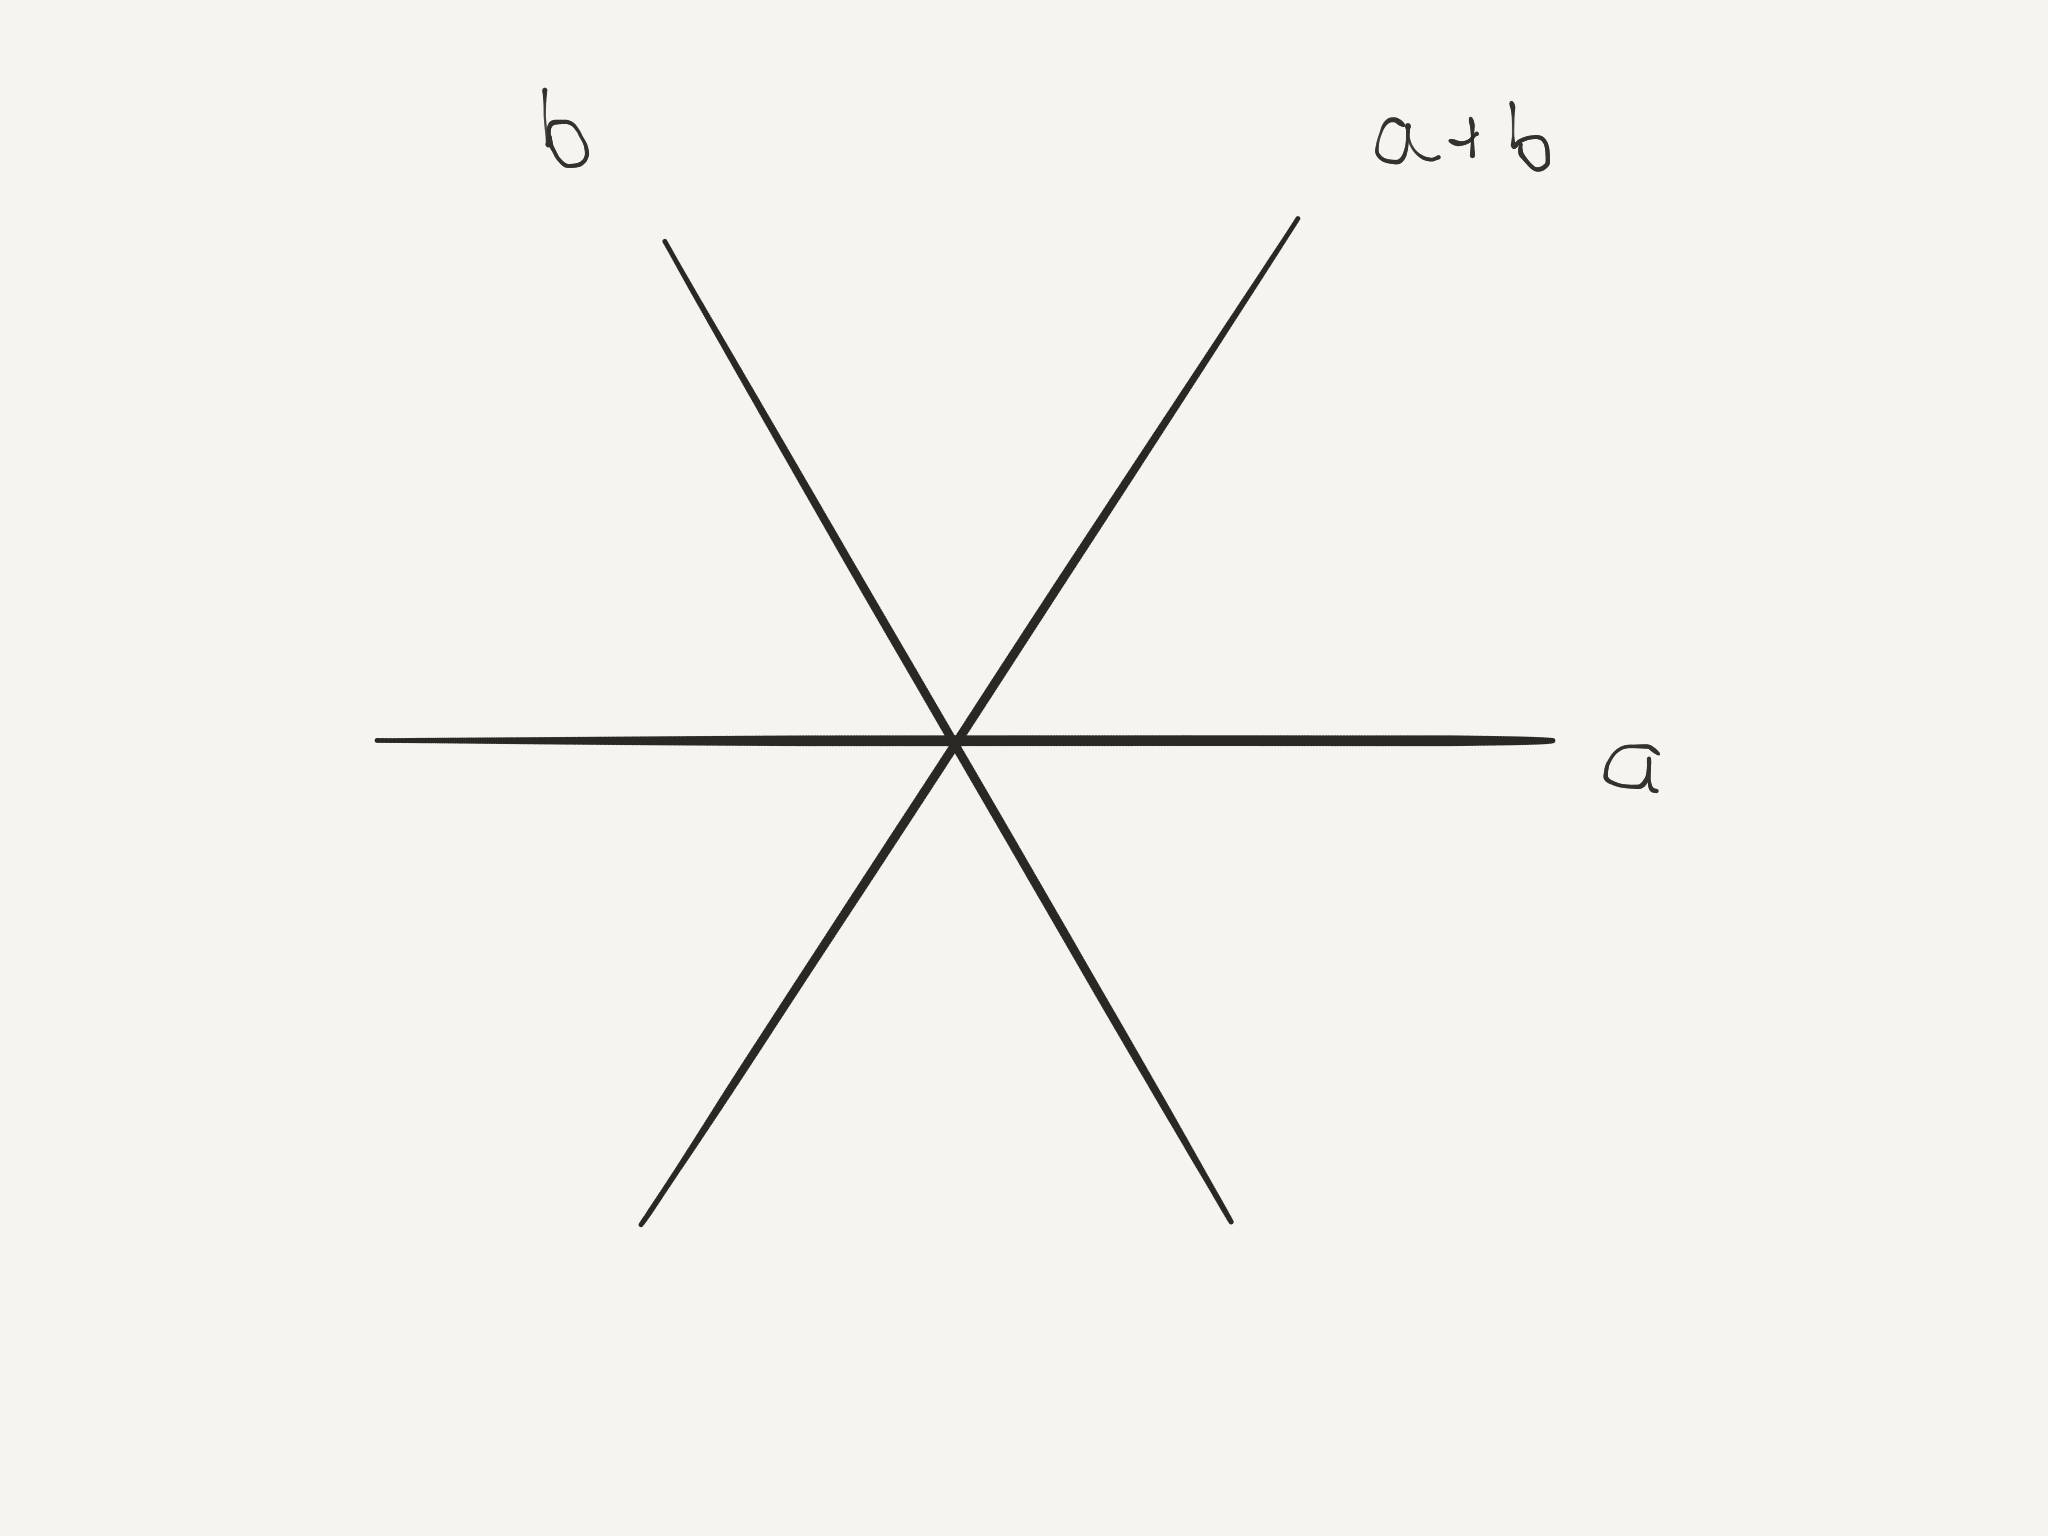
\includegraphics[scale=.15]{249-14.png}
\]
% In this case $W =  \langle r_a, r_b \rangle = S_3$. 
 \[
 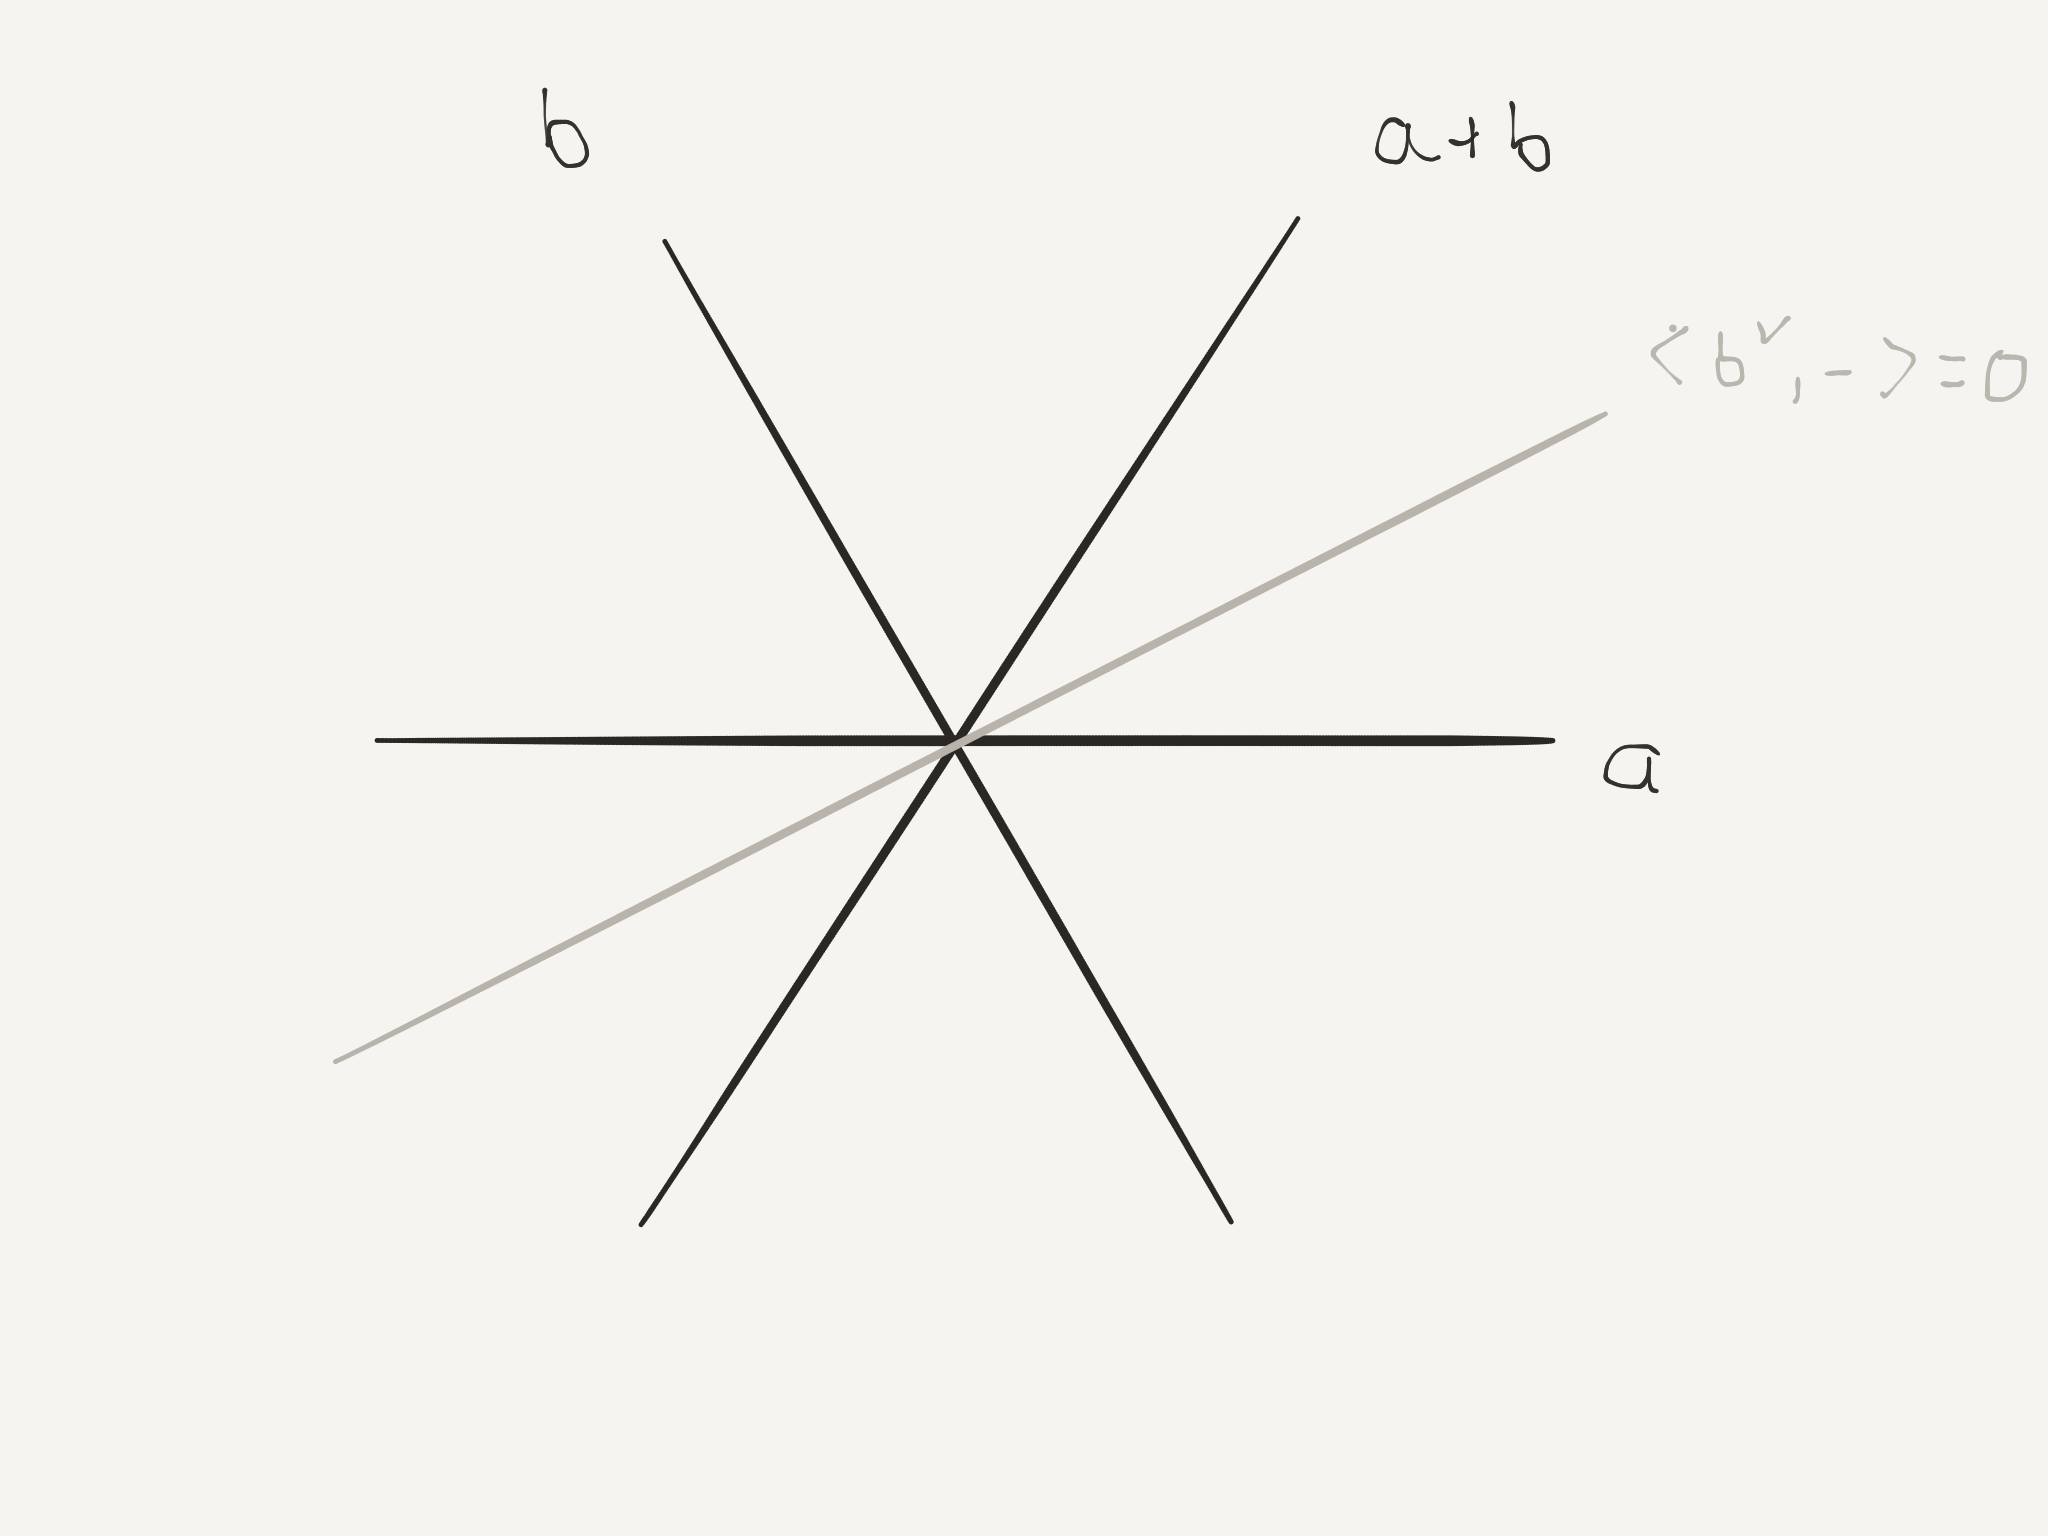
\includegraphics[scale=.15]{249-15.png}
 \]
\end{example}

\begin{example}
For the root system ${\rm{B}}_2 = {\rm{C}}_2$ 
arising from $\SO_5$ and ${\rm{Sp}}_4$
 we have$c^{\vee}=2c$ for $c$ short and $c^{\vee} = c$ for $c$ long (with length $\sqrt{2}$)
 when shortest roots are given length 1; see Figure \ref{fig16}.

\begin{figure}\label{fig16}
\centering
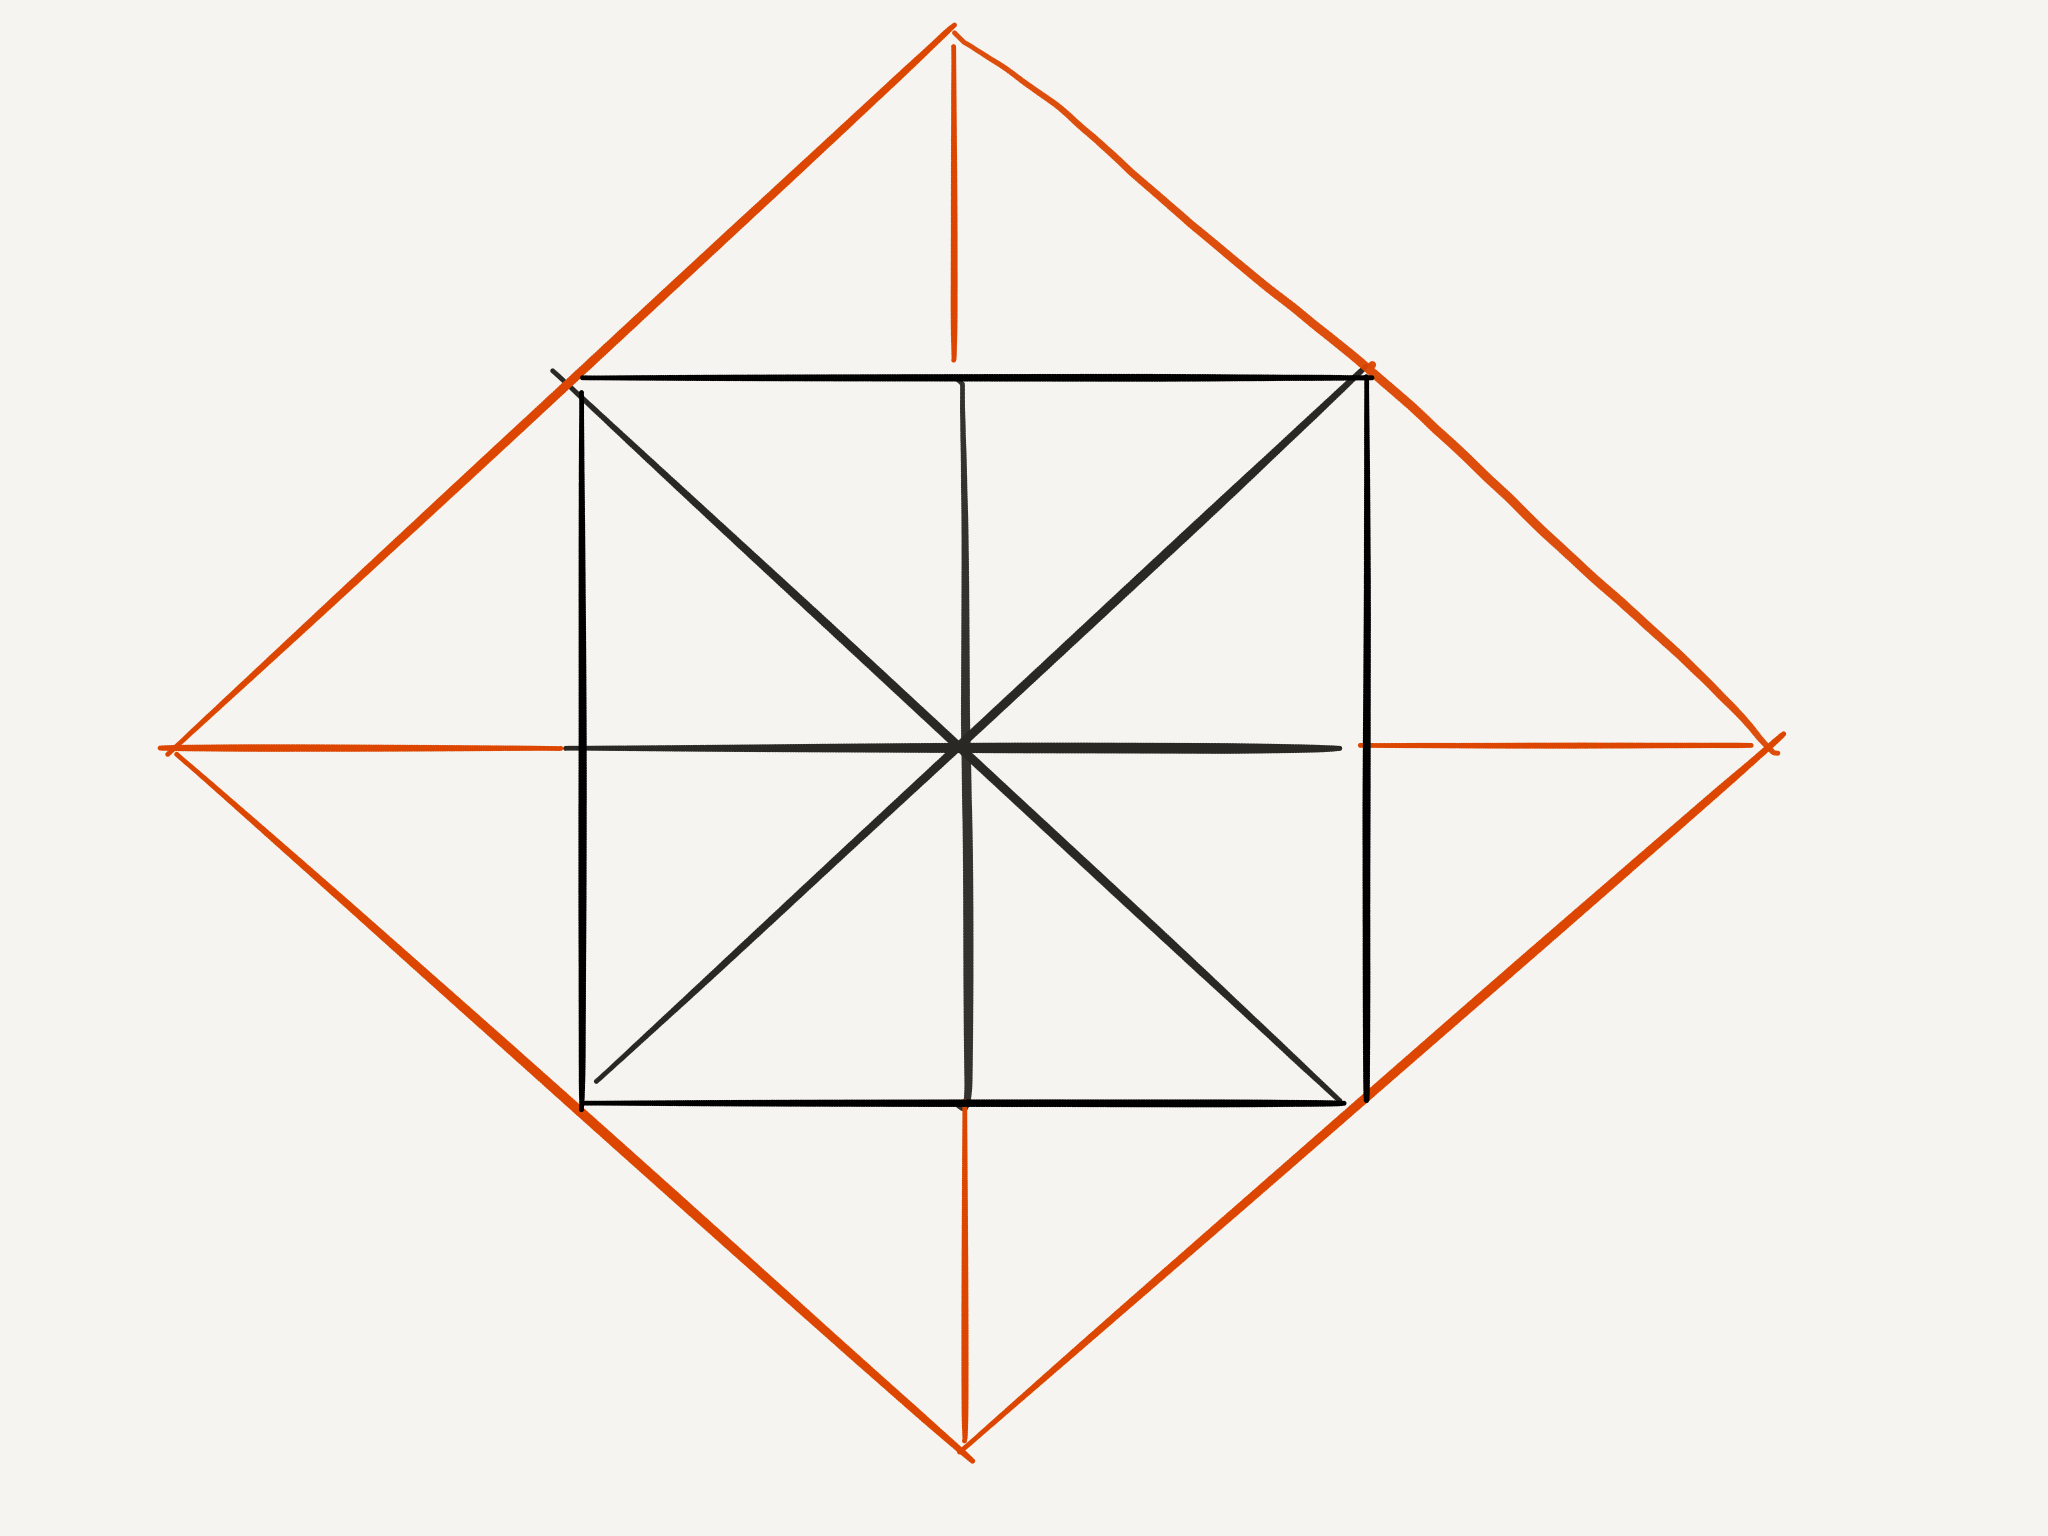
\includegraphics[scale=.2]{249-16.png}
\caption{The root system ${\rm{B}}_2={\rm{C}}_2$ depicted in black (with short roots of length 1)
and its dual in red.}
\end{figure}
\end{example}

Lemma \ref{coroot} implies that $\Phi^{\vee}$ spans $V^*$ over $\Q$, so $(V^*, \Phi^{\vee})$ forms a root system with coroots $(a^{\vee})^{\vee} := a$, called the \emph{dual} root system. 
Since $a/|\!|a|\!|^2$ has length $1/|\!|a|\!|$, passage to the dual root system ``interchanges'' the long and short roots
when there are two root-lengths. 

We have noted and used that the Weyl group acts absolutely irreducibly on the underlying vector space for 
an irreducible root system, but how transitive is the Weyl action on the set of roots? 
The answer is:  as transitive as possible. 
This is the first of the following two important
properties of irreducible root systems:


\begin{proposition}\cite[VI, \S1.3, Prop.\,11]{bourbaki} 
The group $W(\Phi)$ acts transitively on the set of roots of a common length.
\end{proposition}

\begin{proposition}\cite[VI, \S1.4, Prop.\,12]{bourbaki} If an irreducible root system $\Phi$ is reduced, then there are at most two root lengths, and in such cases the ratio of square root-lengths $($long divided by short$)$ is $2$ or $3$.
\end{proposition}

\subsection{Simply connected groups}
Let $\Phi = \Phi(G, T)$ for a split semisimple pair $(G,T)$. 
We have the finite index inclusions 
\[
 \Z \Phi \subset X := {\rm{X}}(T) \subset (\Z \Phi^{\vee})^*
 \]
 with the latter $\Z$-dual to the finite-index inclusion
 \[
 \Z \Phi^{\vee} \subset {\rm{X}}_*(T) =: X^{\vee}.
 \]
 (Recall that coroots rationally span the dual $\Q$-vector space.) 
 Hence, there are only finitely many possibilities for ${\rm{X}}(T)$, namely
 the intermediate groups between $\Z \Phi$ and  $(\Z \Phi^{\vee})^*$. 
 The lattice $\Z \Phi$ is denoted $Q$ and called the {\em root lattice},
 and the dual lattice $(\Z \Phi^{\vee})^*$ is denoted $P$
 and called the {\em weight lattice} (``poid'' is French for ``weight''). 
 
 We have seen that the formation of $\Phi(G, T)$ is invariant under {\em central} isogeny (but not under general isogenies; recall the exceptional isogeny
${\rm{SO}}_{2n+1} \rightarrow {\rm{Sp}}_{2n}$ in characteristic 2;
we will later see that ${\rm{SO}}_{2n+1}$ has root system B$_n$
whereas ${\rm{Sp}}_{2n}$ has root system C$_n$, and these are not isomorphic
for $n > 2$). 
 
 
 For any $(G, T)$ and intermediate lattice $Q \subset X' \subset {\rm{X}}(T)$,
 the corresponding finite subgroup $\mu \subset T$ corresponding to the finite quotient ${\rm{X}}(T)/X'$
 is {\em central} in $G$ since it is killed by all roots (as the restriction $\Phi|_{\mu} \subset
 {\rm{X}}(\mu) = {\rm{X}}(T)/X'$ is trivial since $Q \subset X'$).  Hence, 
 the central quotient $G/\mu$ with split maximal torus $T/\mu$ has root system $\Phi$
 realizing $X'$ as the character lattice for $T/\mu$. 
A calculation similar to that
in Example \ref{rootex} shows that ${\rm{X}}(T/Z_G) = Q$. Furthermore, $Z_G$ is Cartier dual to $X/Q$. 
 
 In the proof of Proposition \ref{rsrd} it is shown that
 $r_{a^{\vee},a}(b^{\vee}) = r_a(b)^{\vee} \in \Phi^{\vee}$ for all
 $a, b \in \Phi$, so for $X$ equal to either of the two extremes $P$ and $Q$ the 4-tuple
 $(X, \Phi, X^{\vee}, \Phi^{\vee})$ really is a root datum.  
 Hence, the Existence Theorem ensures that both extremes arise
 from actual pairs $(G, T)$, so taking $X = P$ then implies by the preceding
 considerations that {\em every} group $X$ between $P$ and $Q$ does arise
 from some split pair $(G, T)$. 
 
 To summarize, for a central isogeny $G \twoheadrightarrow \ol{G}$ satisfying $T \twoheadrightarrow \ol{T}$
  we have ${\rm{X}}(\ol{T}) \hookrightarrow {\rm{X}}(T)$ with finite index, and under central isogenies $X$ moves 
around between $Q$ and $P$ exhausting
all possibilities, with $P$ being the ``biggest'' possibility and $Q$ the smallest.

\begin{definition}\label{pi1def} A split connected semisimple $k$-group $G$ 
is \emph{simply connected} if $X=P$ (equivalently, $\Phi^{\vee}$ spans ${\rm{X}}_{\ast}(T)$), 
and the \emph{fundamental group} of $G$ is the Cartier dual of $P/X$.   More generally, 
a connected semisimple $k$-group is {\em simply connected} when $G_{k_s}$ is so. 
\end{definition}

There are a few reasons that these are appropriate definitions.  Firstly,
if $k = \CC$ then $\pi_1(G(\CC)) = {\rm{Hom}}(P/X, \CC^{\times})$ (the essential case is $X=P$). This can
be proved in at least two ways:  using maximal compact subgroups and Lie theory
(see \cite[Prop.\,D.4.1]{luminy})
or using the Riemann Existence Theorem that finite-degree covering spaces of the analytification
of a finite type $\CC$-scheme have a unique compatible finite \'etale algebraizations
\cite[Exp.\,XII, Thm.\,5.1]{SGA1}
Beware however that this algebraic definition is not compatible with the usual one for real Lie groups. 
For instance, $\SL_2(\R) = \SO_2(\R) \times \R^2$ as manifolds, so $\pi_1(\SL_2(\R)) = \Z$, but $\SL_2$ is 
``simply connected'' as a
connected semisimple $\R$-group. 

 Next, and perhaps more compellingly,
 if $G$ is simply connected then it has a mapping property with respect to central covers
 that is reminiscent of the classical definition of being simply connected
 and doesn't refer to a maximal torus:
  
 \begin{proposition}\label{splitcover}
 Let $G$ be a connected semisimple $k$-group that is simply connected.
 For any $k$-homomorphism $f:G \rightarrow H$  to  a smooth affine $k$-group and $H' \twoheadrightarrow H$ 
a central extension of $H$ by a $k$-group scheme
$\mu$ of multiplicative type, there exists a unique $k$-homomorphism $f':G \rightarrow H'$ lifting $f$: 
\[
\xymatrix{
& H' \ar@{->>}[d] \\
G \ar@{.>}[ur]^{\exists ! } \ar[r] & H
}
\]
\end{proposition}

Before we prove this result, 
we note that the case $H=G$ subsumes the definition of ``simply connected'' 
in the split case \emph{granting} the Existence Theorem, since 
if $G$ is connected semisimple and split then we can apply the mapping property over
$k$ with $H=G$ and $H' \rightarrow 
H$
the central isogenous cover of degree $[P:X]$ corresponding to the root datum using character lattice $P$
to get a homomorphic section, forcing $[P:X]=1$ (i.e., $G$ is simply connected).  
The mapping property over $k$ similarly forces $G$ to be simply connected {\em without}
a split hypothesis, using Corollary \ref{sccover} below.

\begin{proof} The uniqueness of such a lift follows from $G$ being perfect and smooth. Indeed, the difference between any two lifts $G \rightarrow H'$ lands in $\ker(H' \rightarrow H)$, which is central in $H'$. The centrality implies that this difference is actually a group homomorphism. But since $G =\Cal{D}G$, 
an abelian quotient of $G$ must be trivial.

With uniqueness established, Galois descent implies that for the purpose of showing existence, we can assume without loss of generality that $k=k_s$. The advantage of this setting is that $[G(k),G(k)] \subset G$ is Zariski-dense and hence (by reducedness) schematically dense. 

Schematic density is preserved by base change against {\em any} $k$-algebra
(such as the artin local ring $k' \otimes_k k'$ for a finite extension $k'$ of $k$), 
so we can use fppf descent to reduce to the existence over $\ol{k}$. (The point of passing to $\ol{k}$ is to guarantee that the underlying reduced scheme of a group scheme of finite type is a subgroup). The schematic density 
ensures he uniqueness of such a lift over bases which are \emph{not} necessarily fields, such as the artin rings that come up for fppf descent from a finite extension of $k$. This uniqueness comes from the same argument as before: the discrepancy of two such lifts would be a homomorphism to a commutative group scheme, and that is trivial
due to the extension of a schematically dense collection of commutator points over any $k$-algebra. 

Now with $k = \ol{k}$, consider the central extension $G' := f^{-1}(H')$ of $G$ by a $k$-group scheme $\mu =
\ker(H' \twoheadrightarrow H)$ of multiplicative type: 
\[
\xymatrix{
G' \ar[d] \ar[r] & H' \ar@{->>}[d] \\
G \ar[r] & H
}
\]
This reduces us to the case $H=G$ and $H'=G'$, and we want to find a homomorphic
section. We can replace $G'$ with $\Cal{D}(G'_{\red})^0$ (as the latter certainly maps onto $G$).
Now we have reduced to the case where $G'$ is perfect, smooth, and connected. If $G'$ were reductive
(hence semisimple) then we would be done since the central kernel
$\mu$ would have to be finite yet the hypothesis on $G$ ensures that it admits no 
central isogeny of degree $>1$ from a connected semisimple group. 
Since $\mu$ is of multiplicative type and the quotient $G'/\mu = G$ is
reductive, the unipotent radical of $G'$ is forced to be trivial. 
\end{proof}

\begin{lemma}\label{sccover}
Let $G$ be a connected semisimple $k$-group.
Up to unique isomorphism, there exists a central isogeny $\pi:\widetilde{G} \rightarrow G$
with connected semisimple $\widetilde{G}$ that is simply connected.  This is initial among
all central extensions of $G$ by a $k$-group scheme of multiplicative type.  In particular,
$\widetilde{G}$ is functorial with respect to isomorphisms in such $G$.
\end{lemma}

We call $\ker \pi$ is the {\em fundamental group} of $G$, recovering Definition \ref{pi1def} for split $G$.

\begin{proof}
The uniqueness assertions permit us to use Galois descent to reduce to the case $k=k_s$, so $G$ is split.
The Existence Theorem then provides a central
isogeny onto $G$ from a simply connected $\widetilde{G}$.  
It suffices to show that for any surjection $q:G' \twoheadrightarrow G$ of
affine $k$-group schemes of finite type with central kernel $\mu$ of multiplicative type,
there is a unique $k$-homomorphism $\widetilde{G} \rightarrow G'$ over $G$.
It is equivalent to say that the central extension $\widetilde{G} \times_G G'$ of
$\widetilde{G}$ by $\mu$ admits a unique section, which in turn is
the special case $H=G$ in Proposition \ref{splitcover}.
\end{proof}

\begin{example}
For $\SL_n$,
\[
\xymatrix@C=0pc{
\SL_n \ar[d] \supset & T =\{\text{diag} \}\ar[d] \\
\PGL_n \supset & \ol{T}
}
\]
we have the finite-index inclusion
\[
{\rm{X}}(\ol{T}) = (\Z^n)^{\Sigma = 0} \hookrightarrow (\Z^n)/\Delta = {\rm{X}}(T).
\]
obtained by the recipe in Example \ref{rootex} 
applied to the derived group $\SL_n$ and central quotient $\PGL_n$ of $\GL_n$.

Explicitly, the description of the character group of the diagonal of $\GL_n$ implies
that for the derived group $\GL_n$
a character of $T$ is of the form 
\[
\begin{pmatrix} t_1 \\ & \ddots \\ & & t_n \end{pmatrix} \mapsto \prod t_i^{a_i}
\]
for $\vec{a} \in \Z^n$ that only matters modulo the diagonal since $\prod t_i = 1$. 
(We are just passing to character lattices on the exact sequence
$1 \rightarrow T \rightarrow \G_m^n \rightarrow \G_m \rightarrow 1$
whose right map is multiplication.) 
Similarly, character of $\ol{T}$ is exactly a map
\[
\begin{pmatrix} t_1 \\ & \ddots \\ & & t_n \end{pmatrix}  \mapsto \prod t_i^{a_i}
\]
that is well-defined (i.e., unaffected by scaling all $t_i$'s against
a common unit) precisely when $\sum a_i = 0$.

Using these explicit descriptions, the set of roots
\[
\Phi = \{ e_i -e_j \mod \Delta \}
\]
spans ${\rm{X}}(\overline{T})$ over $\Z$ (consistent with the fact that $\PGL_n$ has trivial center) and the set of
coroots 
\[
\Phi^{\vee} = \{e_i^{\ast}-e_j^{\ast}\}
\]
spans the dual ${\rm{X}}_{\ast}(T) = ((\Z^n)^*)^{\Sigma=0}$ of ${\rm{X}}(T)$,
affirming that $\SL_n$ is simply connected. 
\end{example}

\subsection{Weyl chambers}
For split reductive $(G,T)$ we have 
\[
W(\Phi(G,T)) \subset \frac{N_G(T)(k)}{Z_G(T)(k)} =: W(G,T)
\]
(all sitting inside $\GL({\rm{X}}(T))$) as the subgroup generated by the reflections $r_a$, where 
\[
W(\Cal{D}(Z_G(T_a)), \Cal{T}_a) = \{1, r_a\} \subset W(G, T). 
\]
We want to prove that this is an equality (and likewise for relative roots $_k \Phi= \Phi(G,S)$ more generally). This will use Euclidean geometry to relate different-looking notions of ``positive systems of roots''. 

We know that $W(G,T)$ acts simply transitively on the set of
Borel $k$-subgroups containing $T$. We'll show that $W(\Phi(G,T))$ acts simply transitively on 
the set of Weyl chambers. So we need to relate Weyl chambers and Borel subgroups, 
and that will go through two notions of ``positive systems of roots''. The punchline 
will be that via the inclusion between the two types of Weyl groups,
they compatibly act simply transitively on ``the same thing'' and hence the inclusion between these
groups is an equality:

\[
\xymatrix{
\left\{ \text{Weyl chambers in ${\rm{X}}(T)_{\R}$} \right\} \ar@{=}[d] &  \{\text{Borel $k$-subgroups} \supset T \} \ar@{=}[d] \\
\left\{\substack{ \text{combinatorial notion of }\\
\text{positive roots $\Phi^+ \subset \Phi$ }\\ \text{using a root basis}} \right\} \ar@{=}[r]^{\text{Theorem}}_{\text{(in Bourbaki)}} & \left\{ \substack{ \text{dynamic notion of } \\ \text{positive roots }\Phi^+ \subset \Phi} \right\}.
}
\]
\begin{remark} The overall method will apply verbatim to pairs $(G,S)$ in general ($S$ a maximal split 
$k$-torus, and using minimal parabolic $k$-subgroups containing $S$ in place of the Borel
$k$-subgroups containing $T$) once we show that 
the subset ${}_k\Phi := \Phi(G,S) \subset {\rm{X}}(S)$ is a root system in its $\Q$-span and 
that the minimal parabolic $k$-subgroups $P \supset S$ have the ``expected'' dynamic characterization
(using $\lambda \in {\rm{X}}_{\ast}(S) \cap \Q \cdot {}_k\Phi$ non-vanishing on all relative roots) to get 
\[
W({}_k\Phi) = \frac{N_G(S)(k)}{Z_G(S)(k)}
\]
inside $\GL({\rm{X}}(S))$,
\end{remark}

To carry out our plan, we shall introduce Weyl chambers and related notions for an {\em arbitrary}
root system $(V, \Phi)$ (possibly reducible or non-reduced) so that we
can apply it later to ${}_k\Phi$ (that we have noted can be
non-reduced for special unitary groups even over $k = \R$). For $a \in \Phi$, let 
\[
H_a := \ker (a_{\R}^{\vee}) \subset V_{\R}
\]
be the hyperplane of $r_a$-fixed points (so $H_a = (\R a)^{\perp} = H_{qa}$ for any $q \in \Q^{\times}$
such that $qa \in \Phi$). The roots $\pm a$ lie in distinct connected components of $V_{\R}-H_a$;
 i.e. $\pm a$ lie on ``opposite sides'' of $H_a$. 

\begin{definition}
A \emph{Weyl chamber} for $(V, \Phi)$ is a connected component of $V_{\R} - \left(\bigcup_{a \in \Phi} H_a \right)$. 
\end{definition}

It is not at all evident a-priori how to describe such connected components in terms of choices
of signs for each root (i.e., which collections of choices correspond to a connected component?),
so this is one reason that passing to $V_{\R}$ in place of $V$ is very helpful:  we can use topological conditions
to define concepts that at the outset would be difficult to describe in explicit purely algebraic terms. 

\begin{theorem}\cite[VI, \S1.5, Thm.\,2]{bourbaki} We have:
\begin{enumerate}
\item $W(\Phi)$ acts simply transitively on the set of Weyl chambers $C$, and each $C$ has the form 
\[
C = \{ v \in V_{\R} \mid \langle v, a_i^{\vee} \rangle > 0 \ \  [\iff (v, a_i) >0] \}
\] 
where $\{a_i\}$ are exactly the non-divisible roots $a$ such that $\partial C \cap H_a$ has non-empty interior in $H_a$ and $a$ is on the same side of $H_a$ as $C$ is. Also, 
\[
\partial C = \bigcup_i (\partial C \cap H_{a_i}),\,\,\,
\overline{C} = \{v \in V_{\R}\,|\, \langle v, a_i^{\vee} \rangle \ge 0.
\]
$($These $H_{a_i}$ are called the ``walls'' of $C$.$)$ 
\item The set $\{a_i\}$ is a $\Q$-basis for $(V, \Phi)$. $($This is called a ``base'' or ``root basis'' or ``set of simple positive/dominant'' roots.$)$ Furthermore, $W(\Phi)$ has a presentation 
\[
W(\Phi) = \langle r_a \mid r_a^2 = 1, (r_ar_b)^{m_{ab}}=1 \rangle_{a,b \in \Delta}
\]
where $\measuredangle(a,b) = \pi-\frac{\pi}{m_{ab}}$, with $m_{ab} \in \{2, 3, 4, 6\}$. $($A group with such a presentation is called a ``Coxeter group''.$)$ 
\end{enumerate}
\end{theorem}

\begin{example}
There are six distinct Weyl chambers for the root system $A_2$.
\[
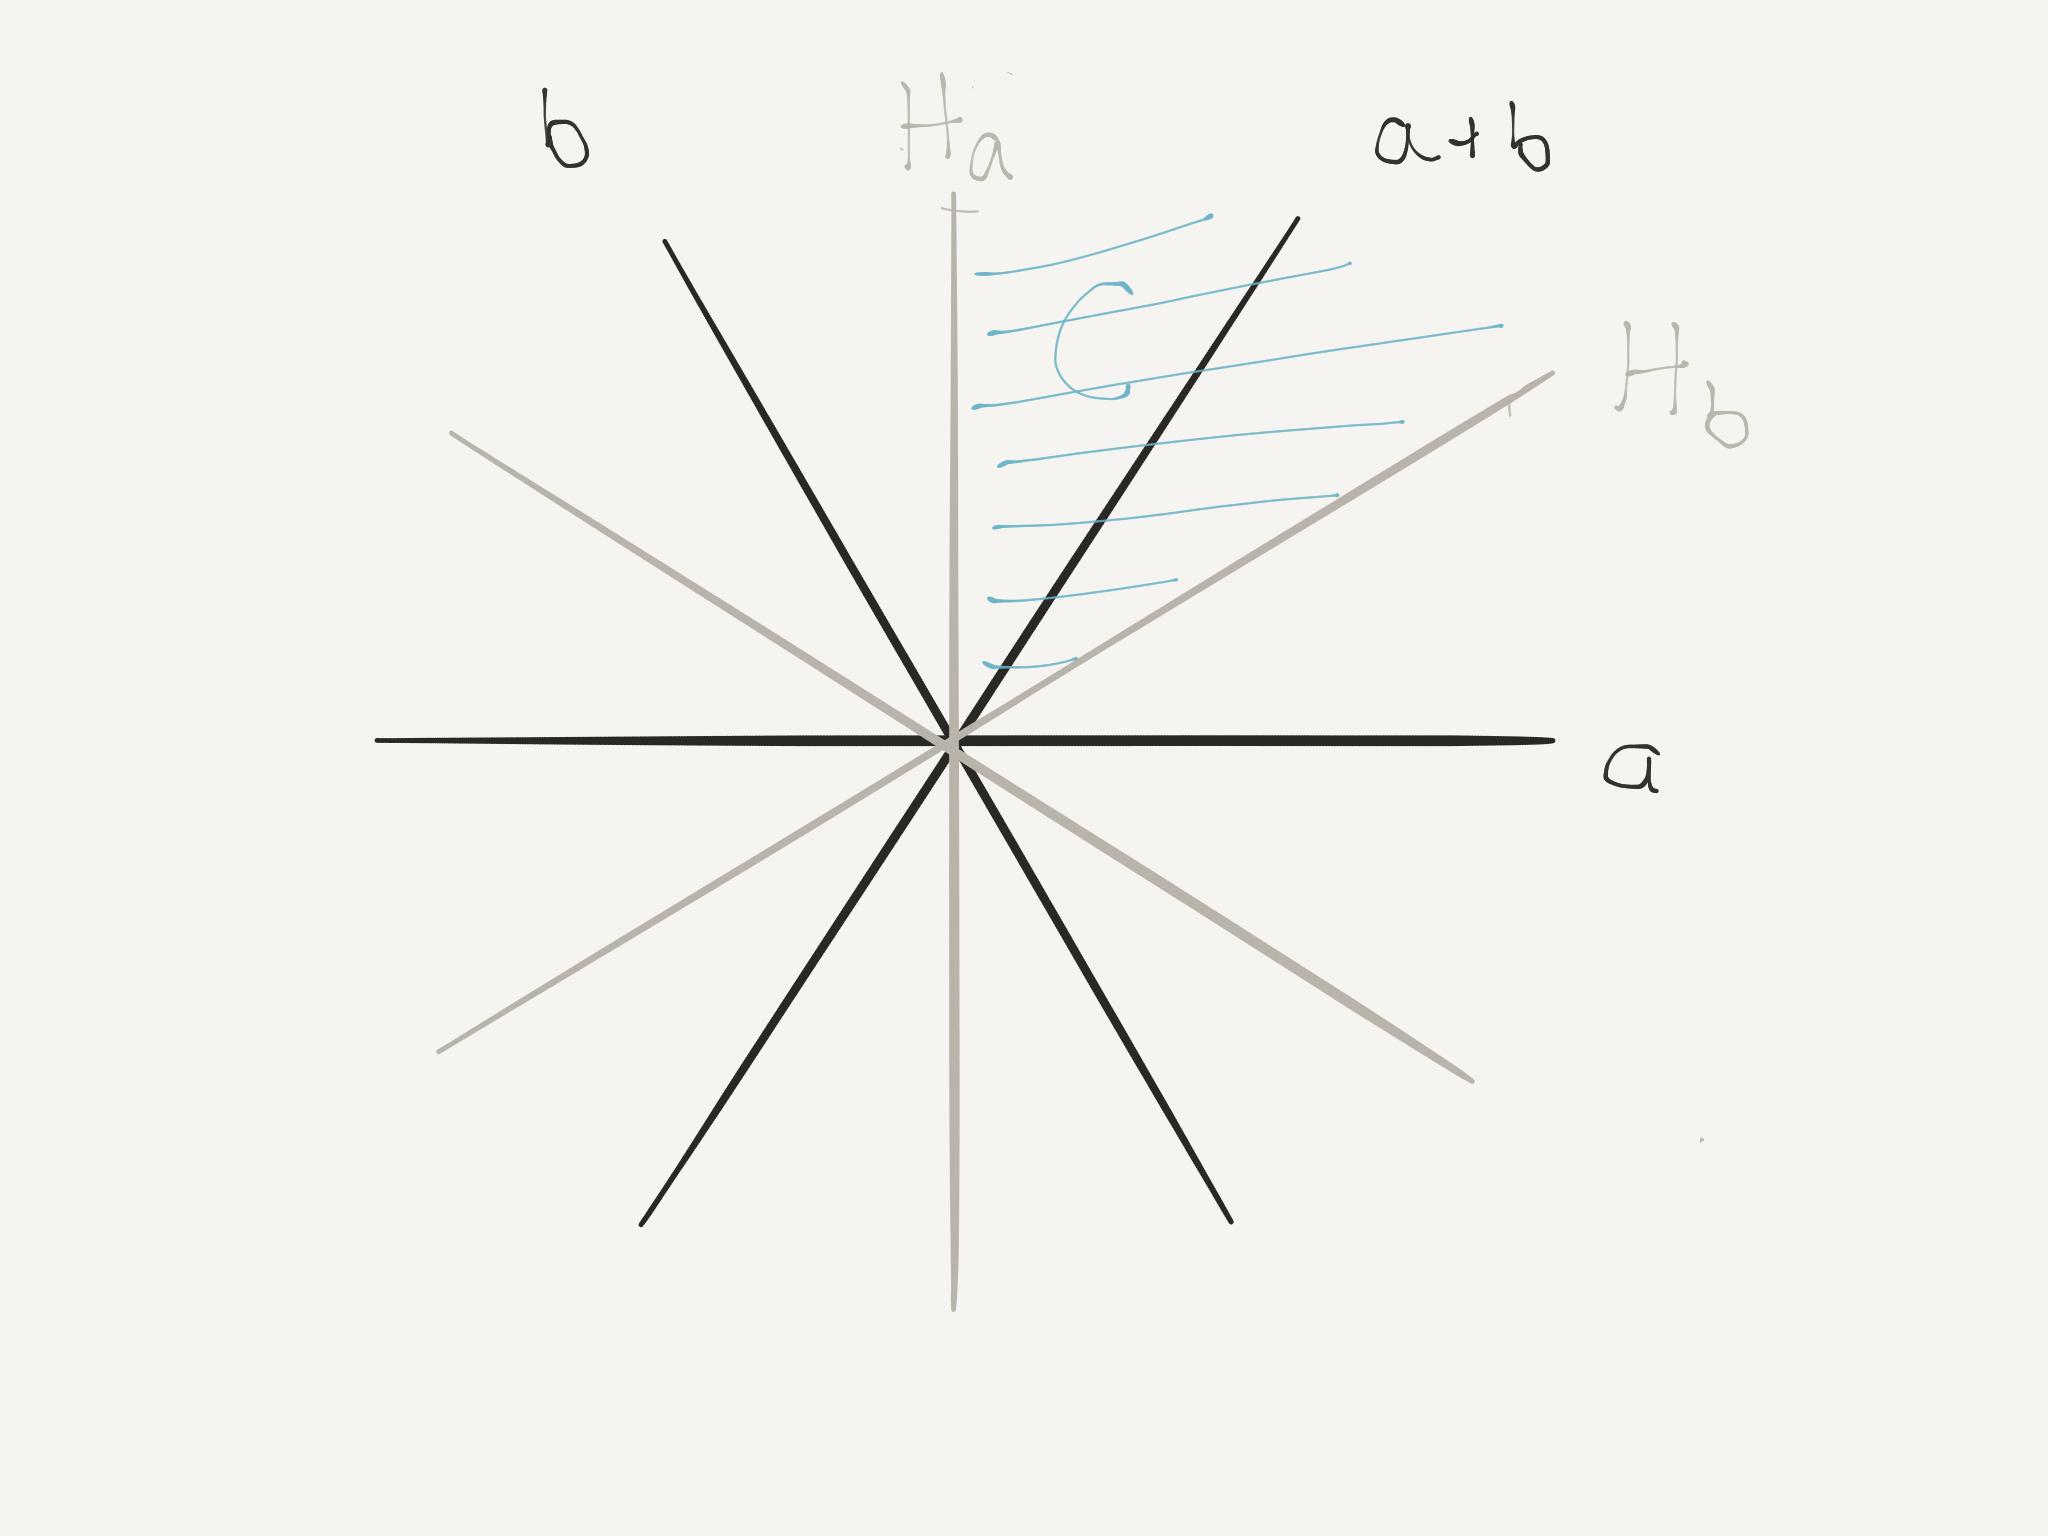
\includegraphics[scale=.2]{249-17.png}
\]
In this case $W = \langle r_a, r_b \rangle = S_3$ with $(r_ar_b)^3 = 1$. 
\end{example}

\begin{example}
For the root system $B_2 =C_2$, there are 8 Weyl chambers. 
\[
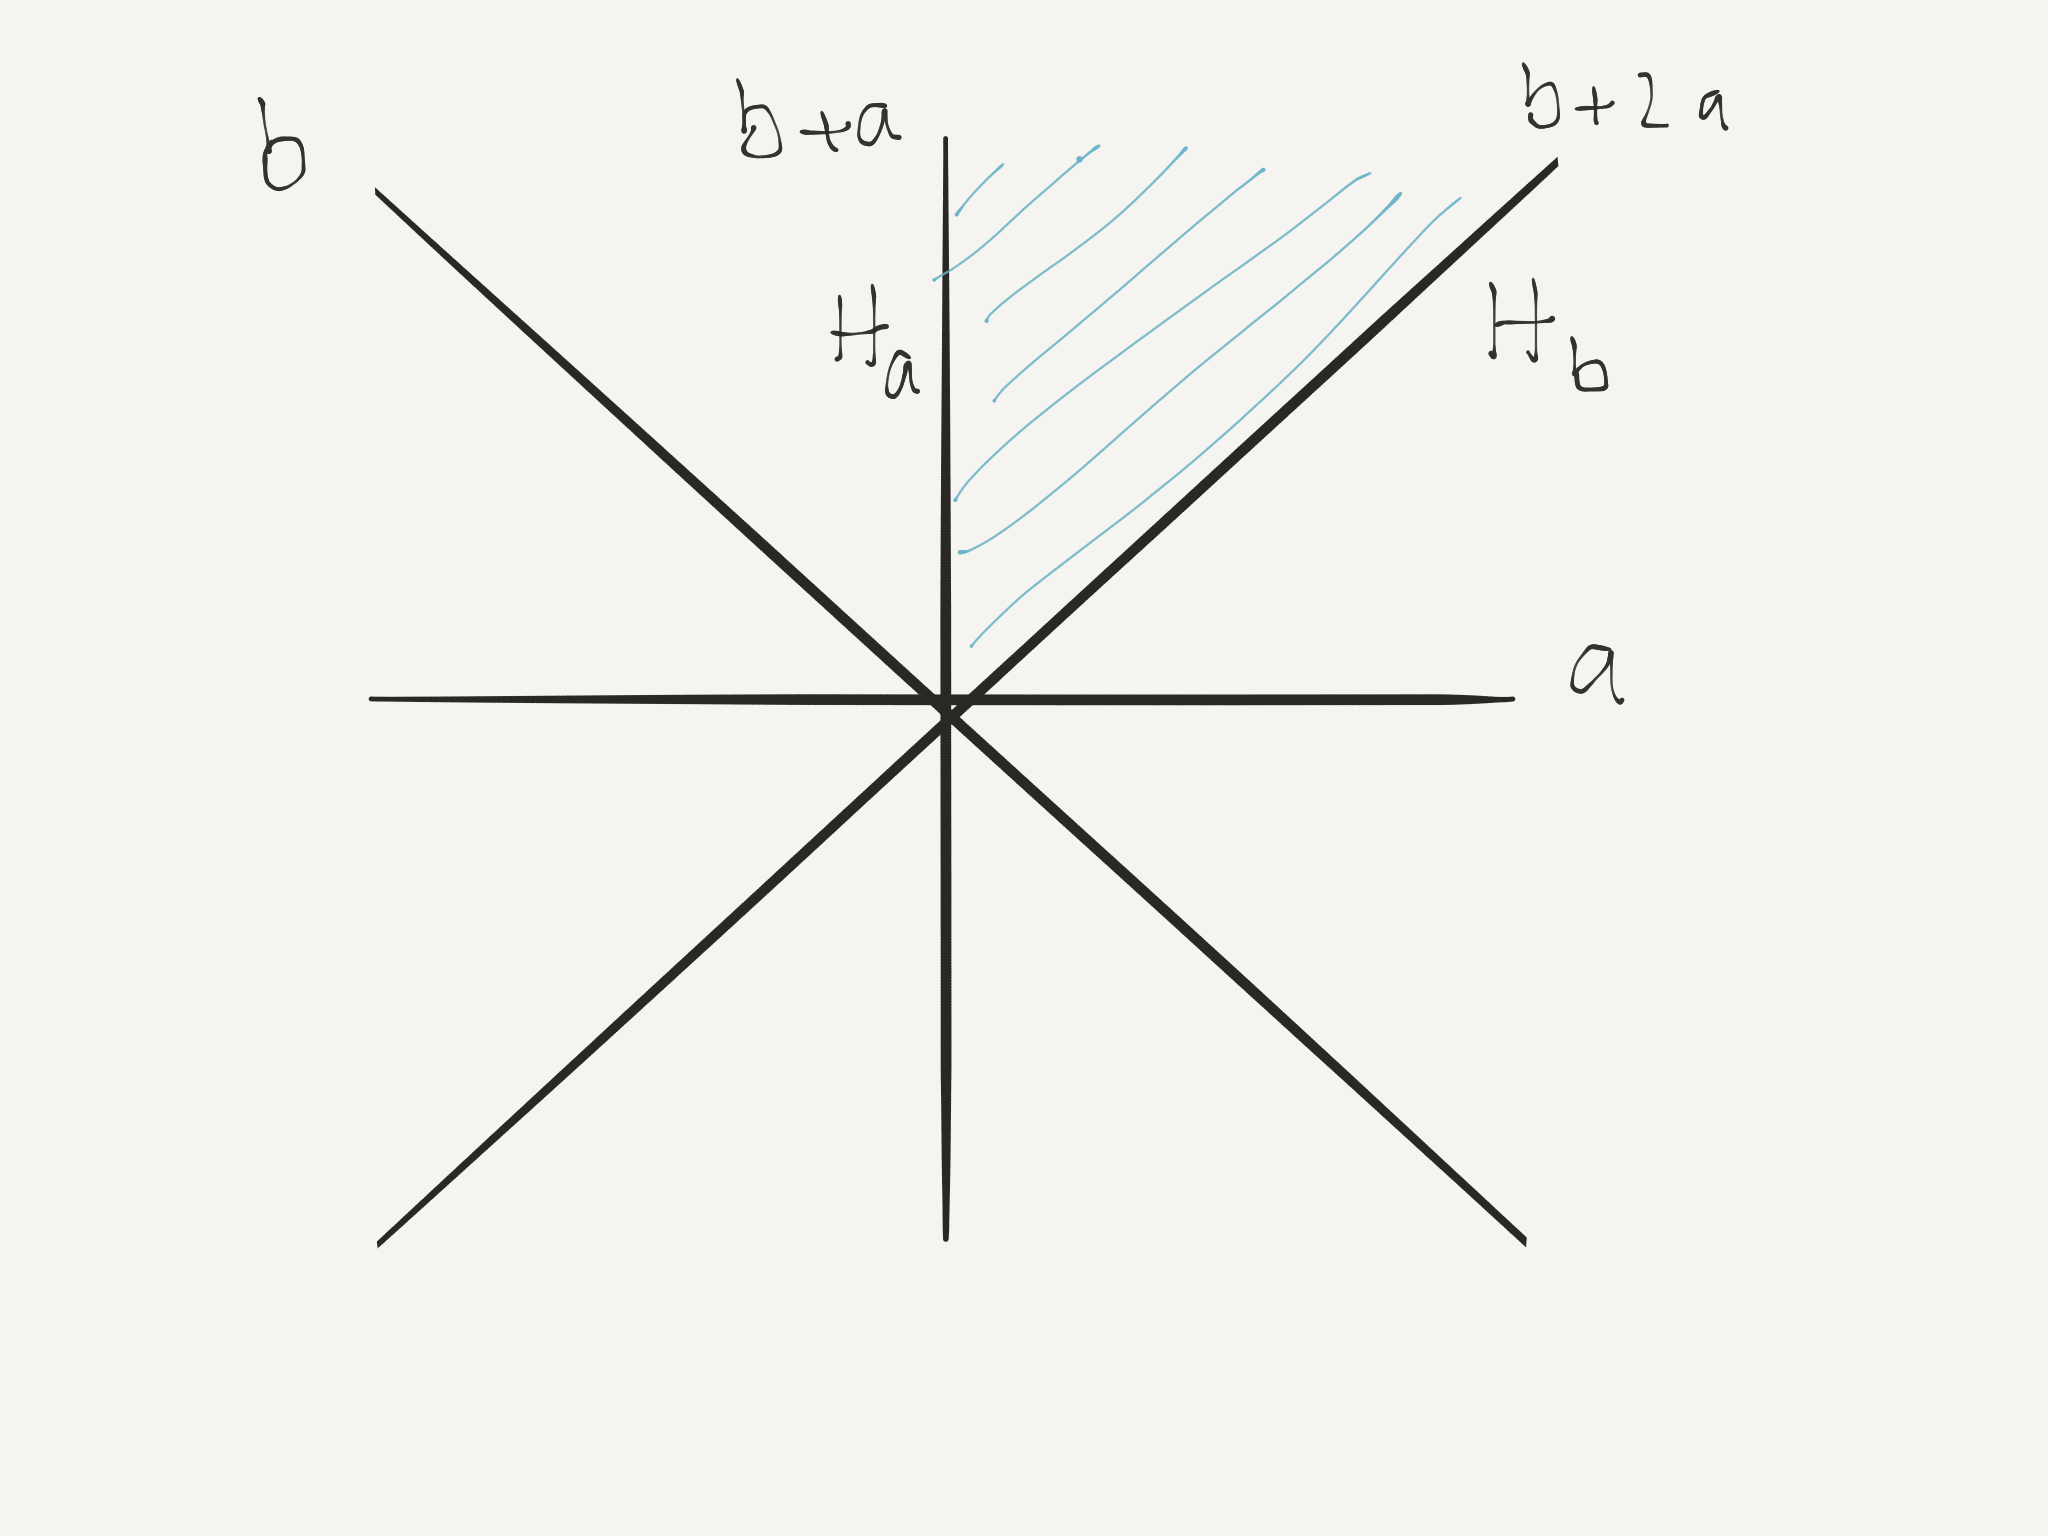
\includegraphics[scale=.2]{249-18.png}
\]
In this case the Weyl group admits a description $W = S_2 \ltimes (\Z/2 \Z)^2$ with $S_2$ generated by 
the reflection $r_a$ in the short simple root
and $(\Z/2\Z)^2$ generated by the reflections $r_b, r_{2a+b}$ in the long positive roots. 
\end{example}

\subsection{Root bases}

\begin{theorem}\cite[VI, \S1.6, Thm.\,3]{bourbaki} If $\Delta \subset \Phi$ is a base, then 
\[
\Phi \subset \Z_{\geq 0} \Delta \sqcup (- \Z_{\geq 0}) \Delta.
\]
\end{theorem}

In other words, when a root is written in terms of a base then all coefficients are integers,
with the nonzero coefficients having the same sign.  In particular,
$\Delta$ is a $\Z$-basis of the root lattice $Q = \Z \Phi$, so
if $(G, T)$ is a split semisimple pair with root system $\Phi$ then $Z_G=1$ if and only if $\Delta$
spans ${\rm{X}}(T)$. 

\begin{definition} The subset $\Z_{\geq 0} \Delta$ is denoted $R_+(C) $ or $R_+(\Delta)$, and called the \emph{positive system of roots} associated to $C$ (or to $\Delta$; we can reconstruct $C$ from $\Delta$). 
\end{definition}

\begin{remark}
The \emph{Coxeter matrix} of $\Phi$ is $(m_{ab})_{a,b \in \Delta}$. This is a symmetric matrix.
\end{remark}

\begin{lemma}\cite[VI, \S1.7, Cor.\,1]{bourbaki} 
A subset $\Psi \subset \Phi$ is a positive system of roots in the above sense if and only if $\Psi$ is closed and 
$\{\Psi, -\Psi\}$ is a partition of $\Phi$. In such cases, the $C$ such that $\Psi = R_+(C)$ is unique. 
\end{lemma}

\begin{example}
If $\lambda \in V^*$ is regular (i.e. non-zero on all roots) then $\Phi_{\lambda > 0}$ is evidently closed and together with its negative partitions $\Phi$. Hence $\Phi_{\lambda > 0} = R_+(C)$ for some $C$. 
In fact, since $\Delta$ is a $\Q$-basis of $V$ \emph{every} $R_+(\Delta)$ has
the form $\Phi_{\lambda >0}$ for some regular $\lambda \in V^*$. (For instance, one could take $\lambda$ to be the sum over the dual basis to $\Delta$.)   

Thus, the dynamic notion of ``positive system of roots''
that we have met  in the study of Borel subgroups of split connected reductive groups
{\em coincides} with Bourbaki's notion defined in terms of Weyl chambers (which in
turn admits a combinatorial characterization in terms of closedness and giving a partition up to signs). 
\end{example}

Now we return to studying $\Phi = \Phi(G,T)$ for a split reductive pair $(G,T)$. We already know that there is a bijection
\begin{align*}
\{\text{Borels} \supset T\} & \leftrightarrow \{ \Phi^+ \subset \Phi\} \\
B & \mapsto \Phi(B,T)
\end{align*}
with compatible actions of $W(G,T)$ on the set of Borels containing $T$
and of $W(\Phi)$ on the set of positive systems of roots. Each action is simply transitive:
for the left side this uses the general $k$-rational conjugacy results that we have already proved and that 
\[
N_G(T)(k)\cap B(k) = Z_G(T)(k),
\]
(a special case of equality $N_G(S)(k) \cap P(k) = Z_G(S)(k)$ for $S$ a maximal split torus and $P$ a minimal parabolic $k$-subgroup containing $S$). For the right side, the result
expresses the fact from Bourbaki that $W(\Phi)$ acts simple transitivity on the set
of Weyl chambers. Hence, we get the desired equality of Weyl groups!

\medskip

\noindent \textbf{Interesting uses of $\Delta$.}
For inductive arguments, it is useful to have:

\begin{proposition}
Assume $\Phi$ is reduced. For $a \in \Delta$, 
\[
r_a(\Phi^+-\{a\}) = \Phi^+ - \{a\}.
\]
\end{proposition}

\begin{proof}
We have $\Phi^+ \subset \Z_{\geq 0} \Delta$ and $r_a(x) \in x + \Z a$. All nonzero $\Delta$-coordinate of $r_a(x)$ have the same sign, and only the ``$a$-component'' has changed.  If $x \ne a$ then $x$ has positive coordinate along another element of $\Delta$ (since $\Phi$ is reduced), so the nonzero $\Delta$-coordinates
of $r_a(x)$ must {\em all} be positive.
\end{proof}

Also, we have the following: 

\begin{proposition}\cite[VI, \S1.6, Cor.\,,1]{bourbaki}\label{sumroot}
 For $a \in \Phi^+ - \Delta$, there exist $a', a'' \in \Phi^+$ such that $a = a' + a''$. 
\end{proposition}

This gives an ``additive characterization'' of $\Delta \subset \Phi^+$. It will underlie the proof (in 
Proposition \ref{conndyn})
for reduced $\Phi$ that the Dynkin diagram ${\rm{Dyn}}(\Phi)$ (to be defined in \S\ref{dynsec}) is connected 
if (and only if) $\Phi^+$ is irreducible.\\


\noindent \textbf{Some useful results.} Let $(V, \Phi)$ be a root system. 
We have seen that the Weyl group  $W$ is generated by reflections through root hyperplanes associated
to a root basis $\Delta$ (i.e., reflections in the hyperplanes giving the walls of a Weyl chamber), underlying
a description of $W$ as a (finite) Coxeter group with a presentation given in terms of the Coxeter matrix.
Moreover, for irreducible $\Phi$ we noted earlier
that the $W$-action on $\Phi$ is transitive on the set of roots of a given length. 

Here's an important result that encodes
 a root system in terms of the minimal possible amount of information:

\begin{proposition}\cite[VI, \S1.5, Prop.\,15 and Corollary]{bourbaki}\label{cartandet}
For reduced $\Phi$, $W. \Delta = \Phi$ $($i.e. every root lies in a root basis$)$, and $\Phi$ is determined up to isomorphism by the Cartan matrix $(\langle a, b^{\vee} \rangle)_{a,b \in \Delta}$ in the following strong
sense: if $(V', \Phi')$ is  a reduced root system with root basis $\Delta'$ then 
for any bijection of sets $f \colon \Delta \rightarrow \Delta'$ respecting the 
Cartan matrices, the resulting $\Q$-linear isomorphism
\[
V = \Q^{\Delta} \simeq \Q^{\Delta'} = V'
\]
carries $\Phi$ onto $\Phi'$. 
\end{proposition}

\begin{remark}
The Cartan matrix is generally not symmetric away from the case
when $\Phi$ is simply laced (all roots with the same length).  
%When $\Phi$ is reduced, 
%the transpose is the Cartan matrix of the dual root system relative to the associated coroot basis;
%see Remark \ref{corootbasis}.
%\end{remark}
%
%\begin{remark}
The Dynkin diagram
$\Dyn(\Phi)$ will be a useful visual way to encode the same information
as in the Cartan matrix or Coxeter matrix.
\end{remark}

Here is a natural question, leading us to the notion of ``associated coroot basis'' (in the reduced case).
First, some setup.  Suppose $\Delta$ is a root basis of $\Phi$,
with associated positive system of roots
$\Phi^+$, so we can write $\Phi^+ = \Phi_{\lambda>0}$ for some regular $\lambda \in V^*$. (Of course $\lambda$ is not unique.) Choose a $W$-equivariant identification $V \simeq V^*$ via a symmetric positive-definite 
$W$-invariant  bilinear form $B$ as usual.

The linear form $\lambda \in V^{\ast}$ corresponds
to some $v \in V = (V^{\ast})^{\ast}$.  This $v$ is regular for $\Phi^{\vee}$
since $\langle v, a^{\vee} \rangle = \langle a, \lambda \rangle \cdot (2/B(a,a))$.
Thus, we can form a positive system of coroots $(\Phi^{\vee})^+ := (\Phi^{\vee})_{v>0}$. 
Our question is this:
can the root basis corresponding to $(\Phi^{\vee})^+$ be described directly in terms of $\Delta$ (without reference
to the auxiliary non-canonical choice of $\lambda$)? 

The answer is \emph{yes} when $\Phi$ is reduced: the root basis (usually called a ``coroot basis'')
 is $\Delta^{\vee} := \{ a^{\vee} \}_{a \in \Delta}$. 
 Detailed hints for how to prove this are given in \cite[Exer.\,1.6.17(i)-(iii)]{luminy}. 
If you think about it, even the fact that $\Delta^{\vee}$ is a root basis for $\Phi^{\vee}$ at all
 is not so clear, since the association from roots to coroots is generally not additive. 
 The Cartan matrix of $\Phi^{\vee}$  relative to $\Delta^{\vee}$ is the transpose of that for $(\Phi, \Delta)$. 
(The reducedness hypothesis cannot be dropped:
if $\Phi$ is \emph{not} reduced, say $b=2a$ then $a^{\vee} = 2 b^{\vee}$, so $a^{\vee}$ cannot be in a root basis since elements of root bases are non-divisible.) 


The root lattice and weight lattices can be explicitly described in terms of $\Delta$ and $\Delta^{\vee}$ respectively:
\[
Q = \Z \Phi = \bigoplus_{a \in \Delta} \Z a
\]
and the dual lattice 
\[
P = (\Z \Phi^{\vee})^* = \bigoplus_{b \in \Delta} \Z(b^{\vee})^*, 
\]
where $\{(b^{\vee})^*\}$ is the dual basis in $V$ to the $\Q$-basis $\Delta^{\vee}$ of $V^*$. 
Clearly the matrix
of the inclusion $Q \hookrightarrow P$ with respect to these bases is the Cartan matrix. 
The group structure of $P/Q$ (hence of the center in the simply connected
case, and of the fundamental group in the adjoint case) is given
in the extensive Tables at the end of \cite{bourbaki}. 

\begin{definition}
We call $(b^{\vee})^*$ the \emph{fundamental weights} (with respect to the choice of $\Delta$). These are the ``highest weights'' for the fundamental representations. 
\end{definition}

For split semisimple pair $(G,T)$ we have $Q \subset {\rm{X}}(T) \subset P$.
By the Existence Theorem, we saw just above
Definition \ref{pi1def} that every group $X$ between
$P$ and $Q$ arises as ${\rm{X}}(T)$ for some central isogenous quotient of
such the pair $(G', T')$ satisfying ${\rm{X}}(T')=P$, which is to say for simply connected $G'$  (by definition). 
In particular, the following conditions on $G$ are equivalent:
\begin{itemize}
\item $G$ is simply connected, 
\item $\Delta^{\vee}$ spans ${\rm{X}}_*(T)$ (equivalently, ${\rm{X}}_*(T) = \Z \Phi^{\vee}$), 
\item the natural map $\prod_{b \in \Delta} \G_m \rightarrow T$ defined by
$(y_b) \mapsto \prod b^{\vee}(y_b)$ is an \emph{isomorphism}.
\end{itemize}

\begin{lemma}\label{levisc}
Let $G$ be a connected semisimple group that is simply connected.
For any $k$-torus $T' \subset G$, the connected semisimple groups
$\Cal{D}(Z_G(T'))$ is simply connected. 

In particular, Levi factors of
parabolic $k$-subgroups of $G$ have simply connected derived groups,
and if $G$ has a split maximal $k$-torus $T$ then
for each $a \in \Phi(G, T)$ 
and codimension-$1$ subtorus $T_a := (\ker a)^0_{\rm{red}} \subset T$ 
the subgroup $\mathscr{D}(Z_G(T_a)) = \langle U_a, U_{-a}\rangle$
is $\SL_2$ rather than $\PGL_2$. 
\end{lemma}


\begin{remark}\label{nosc}
The analogue for ``adjoint type'' (i.e. trivial center) is false. For a counterexample, in the split case 
with $T' = (\ker a)^0_{\red}$ the $k$-group $\Cal{D}(Z_G(T'))$ that 
is isomorphic to $\SL_2$ or $\PGL_2$ is always
$\SL_2$ when $G$ is the adjoint-type $\PGL_n$ with $n \geq 3$. 
\end{remark}

The details of the proof of Corollary \ref{levisc} are given in \cite[Exer.\,6.5.2(iv)]{luminy}. 
Here we just sketch the main ideas.

\begin{proof}[Idea of proof] 
Let $T$ be a maximal $k$-torus containing $T'$. 
Without loss of generality $k = k_s$, so $T$ is split.
Hence, $T = \prod_{b \in \Delta} b^{\vee}(\G_m)$. 
For any ``generic'' $\lambda' \in {\rm{X}}_*(T')$ (i.e., pairing non-trivially with all non-trivial
$T'$-weights on ${\rm{Lie}}(G)$) we see by comparison of Lie algebras
that the inclusion of smooth connected $k$-subgroups
$Z_G(T')\subset  Z_G(\lambda')$. 

 The intersection $S:=T \cap (\Cal{D}(Z_G(T')))$ is a maximal $k$-torus
 in $\Cal{D}(Z_G(T'))$ because rather generally if $H$ is a connected linear algebraic $k$-group
 with smooth connected normal $k$-subgroup $N$ (such as $H = Z_G(T')$
 and $N = \mathscr{D}(H)$) then for every maximal $k$-torus $T \subset H$
 the (scheme-theoretic) intersection $T \cap N$ is a maximal $k$-torus of $N$;
 see \cite[Cor.\,A.2.7]{pred} for a (simple and self-contained) proof
 after first trying to make your own proof as an exercise.
 
 The torus intersection $S \subset T = \prod_{b \in \Delta} \G_m$ then turns out to be a subproduct
\[
 T \cap (\Cal{D}(Z_G(T'))) = \prod_{\substack{b \in \Delta \\ \langle \lambda', b \rangle = 0}} \G_m.
\]
One deduces that the elements of $\Delta$ orthogonal to
$\lambda'$ constitute a root basis for the connected
semisimple group $\Cal{D}(Z_G(T'))$ (with its split maximal torus $S$). 
Hence, ${\rm{X}}_{\ast}(S)$ is spanned by the coroots, so $\Cal{D}(Z_G(T'))$ is simply connected. 
\end{proof}

The point is that we're building things \emph{inside} a torus $T$ via intersection, 
and the structure of a $k$-subgroup of $T$ can be probed with cocharacters of $T$. 
This situation cannot be similarly probed by characters, which is informally the
reason that the proof does not adapt to the opposite extreme in which the property
of being simply connected is replaced with the property of having trivial center 
(and we know it really cannot adapt to that property, due to Remark \ref{nosc}). 


\begin{remark} We say that a connected reductive group $G$ over a field $k$ is {\em of adjoint type}
when $Z_G=1$.  The reason for the terminology is that
the inclusion $Z_G \subset \ker {\rm{Ad}}_G$ is an equality of group schemes
for any connected reductive $k$-group $G$. 

This is easy to prove in characteristic $0$ using the faithfulness of the Lie-algebra functor
for connected algebraic groups in characteristic 0 (and Cartier's theorem on the smoothness
of algebraic groups over fields of characteristic 0).
But in characteristic $p>0$ this equality of group schemes is 
rather specific to the reductive case:
there are smooth non-commutative 2-dimensional unipotent groups in characteristic $p$ with trivial adjoint representation!  These matters are discussed fully in Appendix \ref{zgstr}. 

The hard part of the proof that $Z_G = \ker {\rm{Ad}}_G$ is to show that 
the conjugation action on $\ker {\rm{Ad}}_G$ by a maximal torus 
is trivial.  That would imply $\ker {\rm{Ad}}_G$ is contained
in the schematic centralizer of $T$, 
but $Z_G(T)=T$ and the kernel of ${\rm{Ad}}_G|_T$ is easily described in terms of roots
by the very definition of roots.
\end{remark}


\subsection{Dynkin diagrams}\label{dynsec}

\begin{definition}
Let $(V, \Phi)$ be a reduced root system with root basis $\Delta$. The \emph{Dynkin diagram} of $\Phi$ is an ``oriented weighted graph'' (some edges having multiplicity and direction):
\begin{itemize}
\item the vertex set is $\Delta$, 
\item an edge joins distinct $a,b \in \Delta$ precisely when $\langle a, b^{\vee} \rangle \neq 0$ (equivalently, 
$\langle b, a^{\vee} \rangle \neq 0$; i.e. $a$ and $b$ are not orthogonal), 
\item if an edge joins $a$ and $b$ (so by non-orthogonality they
lie in the same irreducible component and hence have an intrinsic
ratio between their lengths), and we relabel
so that $|\!|a|\!| < |\!|b|\!|$ in case of distinct root lengths, then the edge multiplicity is
\[
 \frac{\langle b, a^{\vee} \rangle }{\langle a, b^{\vee} \rangle} = \frac{||b||^2}{||a||^2} \in \{1, 2, 3\},
\]
with the direction pointing towards the shorter root when there are distinct root lengths.
\end{itemize}
\end{definition}

\begin{example}
The Dynkin diagrams for A$_2$, B$_2$, and G$_2$ are depicted below. 
\[
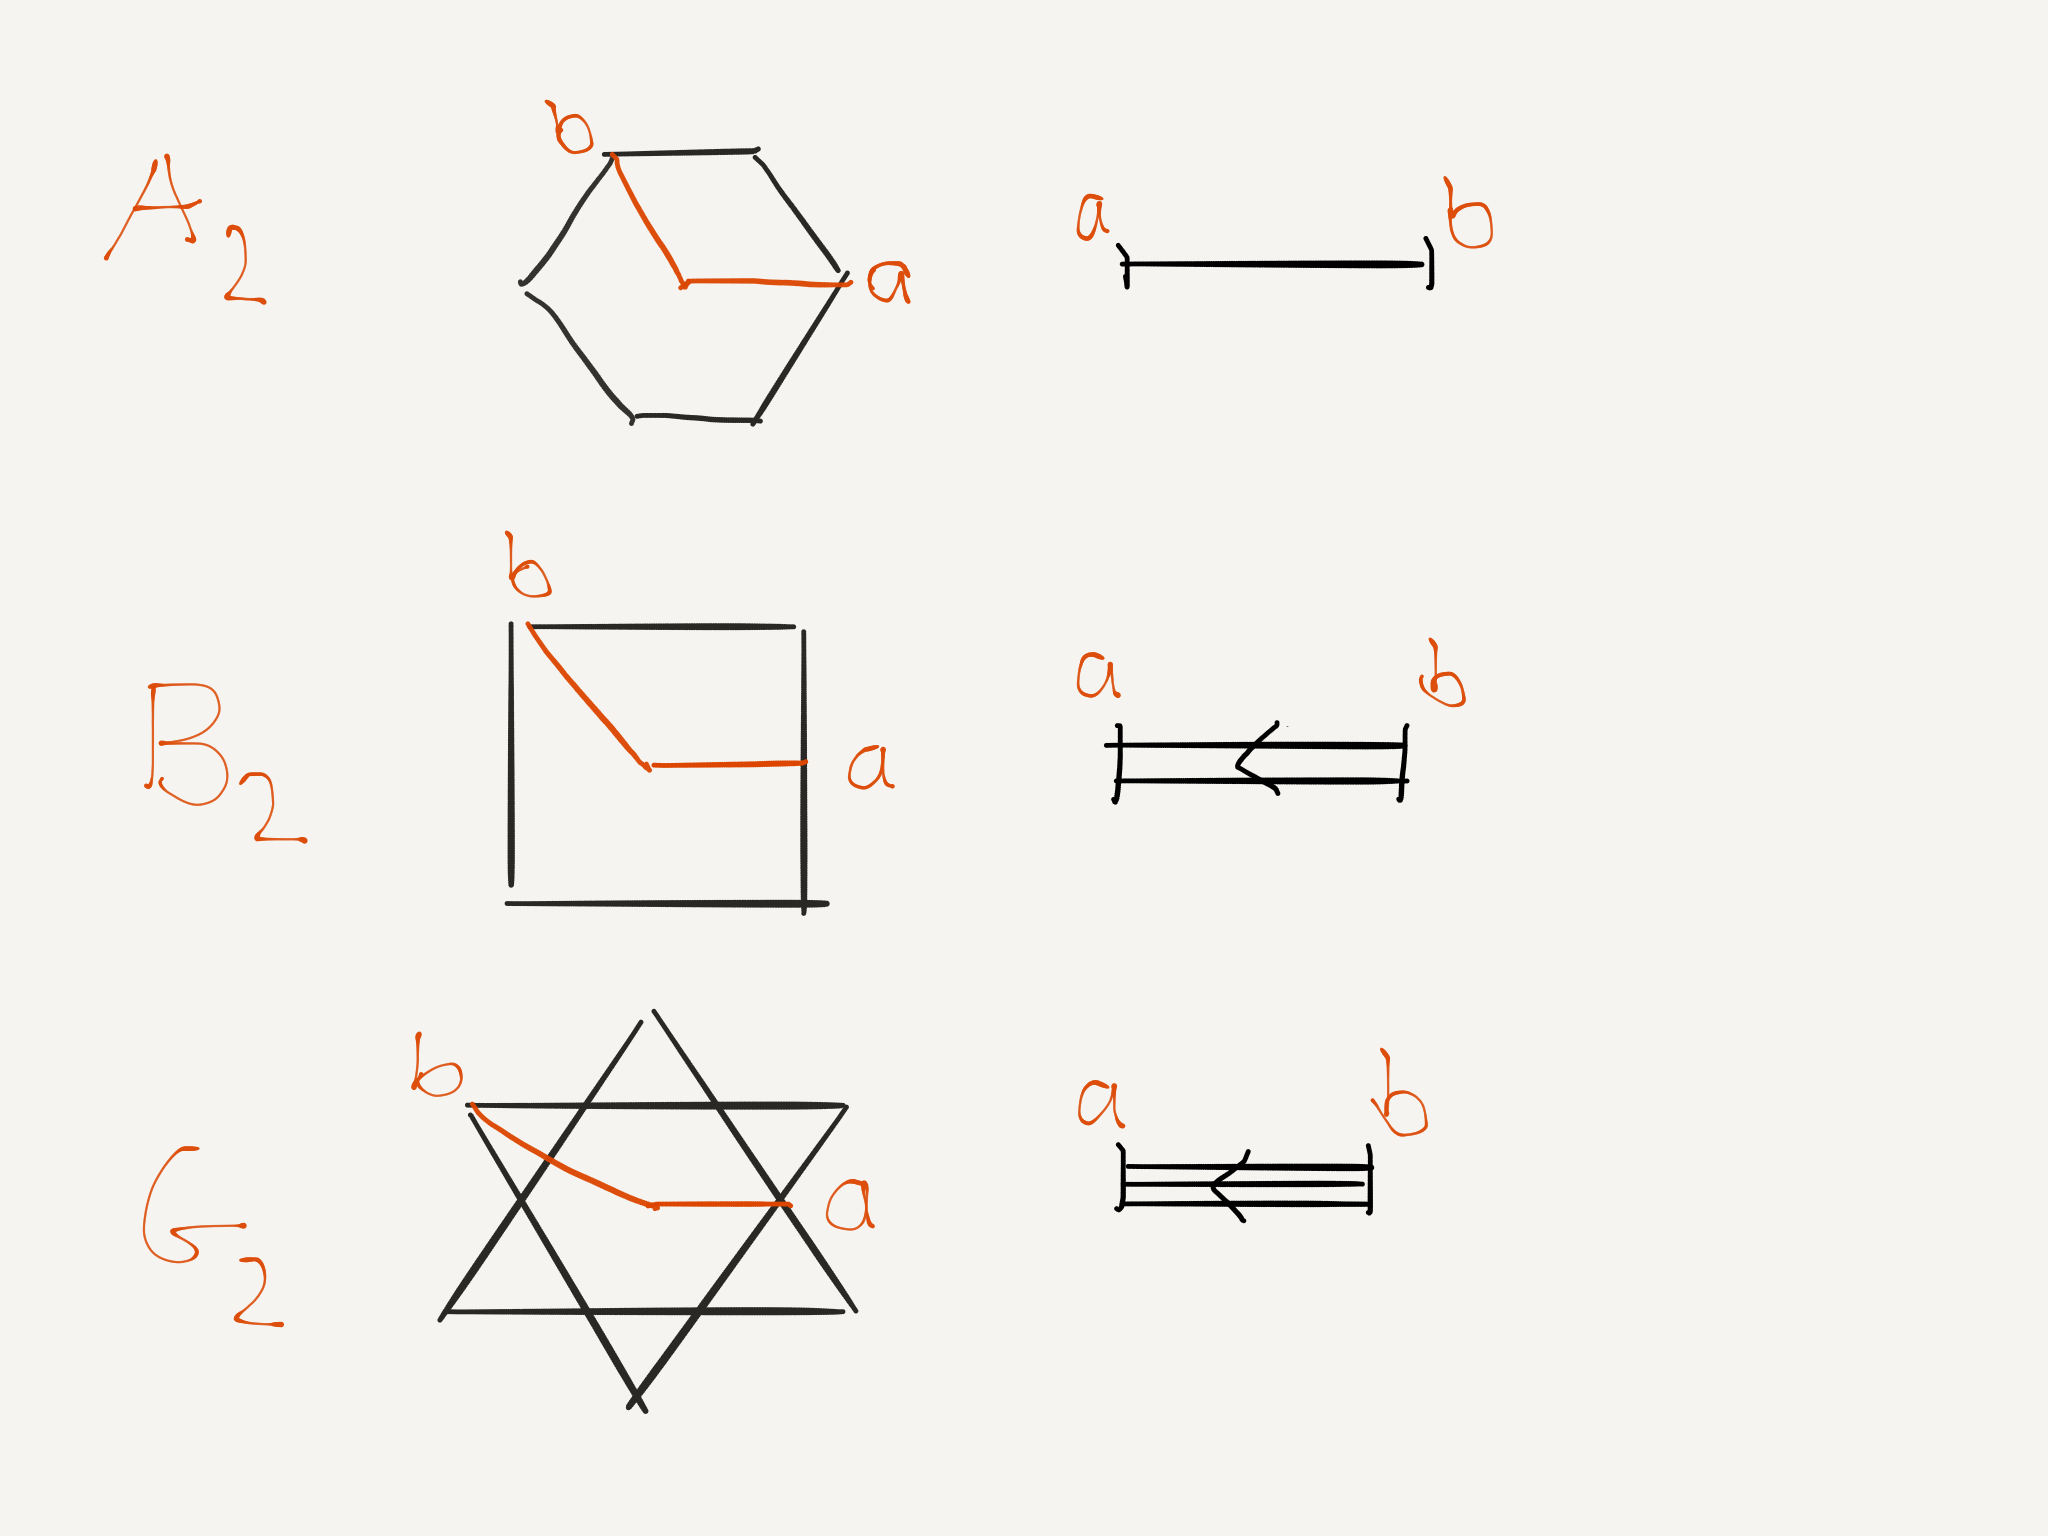
\includegraphics[scale=.25]{249-20.png}
\]
\begin{remark}
The ratio of squared root lengths as above is the number of times $a$ can be added to $b$ 
to obtain another root, as is apparent in the figures above. 
\end{remark}
\end{example}

For distinct $a,b \in \Delta$ we have
\[
\langle a, b^{\vee} \rangle = 2 \frac{||a||}{||b||} \cos (\measuredangle (a,b))
\]
(vanishing precisely when $a$ and $b$ are not adjacent vertices).
If $a$ and $b$ are adjacent then $(\Z a + \Z b) \cap \Phi$ is a reduced 
rank-2 root system with root basis $\{a, b\}$ consisting of non-orthogonal roots, so
this rank-2 root system is irreducible. Indeed, if it would be reducible then there are two irreducible components
each of rank 1, giving a root basis consisting of two orthogonal roots, yet all root bases are ``created equal''
through the action of the Weyl group, so they cannot consist of orthogonal roots
since $\{a, b\}$ is a root basis.

By Euclidean plane geometry,
the reduced and irreducible root systems of rank 2 are completely determined in 
\cite[VI, \S3]{bourbaki}.
From inspection of the possibilities we see for non-orthogonal $a,b \in \Delta$ that 
\[
\boxed{ \measuredangle (a,b) = \pi - \frac{\pi}{m_{a,b}} = \begin{cases} 2\pi / 3 & \cdot - \cdot\\ 3 \pi /4 & \cdot \Rightarrow \cdot \\ 5 \pi / 6 & \cdot \Rrightarrow \cdot\end{cases} }
\]
where $m_{a,b}$ is the order of $r_ar_b$. Thus, $\Dyn(\Phi)$ encodes the Coxeter
and Cartan matrices, so it determines $(V, \Phi)$ up to isomorphism by Proposition \ref{cartandet}. 

The Coxeter matrix determines the presentation for $W(\Phi)$ as a finite Coxeter group. These are classified 
in \cite[VI, \S4.1]{bourbaki} when $\Dyn(\Phi)$ is \emph{connected} (permitting
inductive arguments with subdiagrams for making a determination of all
possibilities). By Euclidean geometry \cite[VI, \S4.2]{bourbaki}
 finds a list containing all {\em possibilities} for connected $\Dyn(\Phi)$.
\[
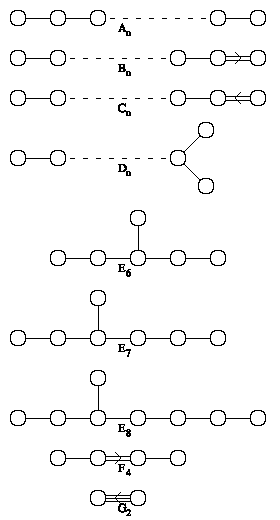
\includegraphics[scale=.75]{249-19.png}
\]
One can directly construct all of these root systems inside suitable $\R^n$'s \cite[VI, \S4.4-4.14]{bourbaki} 
(determining much related information along the way, such as the fundamental weights,
the structure of $P/Q$, etc.), 
so all of these possibilities really occur. 

 In Proposition \ref{conndyn}
we will prove the crucial fact that ${\rm{Dyn}}(\Phi)$ is {\em connected}
whenever the reduced root system $\Phi$ is irreducible (the converse is obvious:
if $\Phi$ is a direct sum of non-empty root systems $\Phi'$ and $\Phi''$
then by orthogonality considerations we see that ${\rm{Dyn}}(\Phi)$
is the disjoint union of ${\rm{Dyn}}(\Phi')$ and ${\rm{Dyn}}(\Phi'')$.
Hence, the above is a list of {\em all} reduced irreducible root systems (up to isomorphism;
note that ${\rm{B}}_2 = {\rm{C}}_2$).

In Appendix \ref{classicalgps}, it is worked out that the root systems of types A, B, C, and D
arise from specific split classical groups:  SL$_{n+1}$ is type A$_n$ ($n \ge 1$),
SO$_{2n+1}$ is type B$_n$ ($n \ge 2$), Sp$_{2n}$ is type C$_n$ ($n \ge 2$),
and SO$_{2n}$ is type D$_n$ ($n \ge 3$).
The equality of root systems ${\rm{B}}_2 = {\rm{C}}_2$ corresponds to a low-rank isomorphism
$\Sp_4/\mu_2 \simeq \SO_5$ explained in linear algebraic terms in \cite[Ex.\,C.6.5]{luminy}. 

Convenient low-rank conventions for some special diagram names
are inspired by isomorphisms or {\em central} isogenies
among low-rank members of the classical families (and also reasonable in terms of the pictures of the graphs).
See \cite[Ex.\,C.6.2, C.6.3, C.6.5]{luminy} for justification of the following isomorphism
or central isogeny claims via calculations with $\Z$-groups  (to make characteristic-free arguments,, 
especially to avoid special treatment of characteristic 2): 
\begin{itemize}
\item define B$_1$ to be A$_1$ because $\PGL_2 \simeq \SO_3$ through ``$\PGL_2$-conjugation'' on 
the 3-dimensional space
$\mathfrak{sl}_2 = \mathfrak{gl}_2^{{\rm{Tr}}=0}$ 
leaving invariant the determinant as a non-degenerate split quadratic form in 3 variables;
\item define C$_1$ to be A$_1$ because $\Sp_2 = \SL_2$ (determinant on the space ${\rm{Mat}}_2$
is a symplectic form in the ordered pair of columns in $k^2$);
\item define D$_2$ to be ${\rm{A}}_1 \times {\rm{A}}_1$ because
the action of $\SL_2 \times \SL_2$ on the 4-dimensional space ${\rm{Mat}}_2$
through left and right multiplication (i.e., $(g,g')M = gM{g'}^{-1}$) visibly leaves invariant 
the non-degenerate split quadratic form $\det: {\rm{Mat}}_2 \rightarrow k$ in 4 variables, 
thereby defining a homomorphism
$\SL_2 \times \SL_2 \rightarrow \SO({\rm{Mat}}_2, \det) = \SO_4$ that is
the quotient by the central diagonally embedded $\mu_2$;
\item define D$_3$ to be A$_3$ because  by definition of the determinant
in terms of top exterior powers, the natural action of $\SL_4$ on 
the 6-dimensional $V = \wedge^2(k^4)$ leaves {\em invariant} the natural non-degenerate
split quadratic form $V \rightarrow \wedge^4(k^4)$ defined by $q(v) = v \wedge v$,
yielding a homomorphism $\SL_4 \rightarrow {\rm{O}}_6^0 = \SO_6$ that is the quotient by the central 
$\mu_2$. 
\end{itemize}

The non-reduced  irreducible root systems should not be overlooked! To describe the possibilities, we
first need to record a few facts concerning reduced root systems.  A
reduced irreducible root system such that (i) some ratio of squared root
lengths is equal to 2 and (ii) all roots of some length are pairwise orthogonal
(ruling out F$_4$, whose diagram has a pair of adjacent short roots and a pair of adjacent long roots) must 
be either B$_n$ and C$_n$ for some $n \ge 1$, and these types do satisfy
both conditions (using inspection of the construction to verify (ii)).
Moreover, an inspection of the Plates at the end of \cite{bourbaki} shows the curious fact that 
the root systems C$_n$ ($n \ge 1$, where C$_1$ means A$_1$)
are precisely the reduced irreducible root systems for 
which there is a root that is non-trivially divisible inside $P$:
its long roots are twice primitive vectors in the weight lattice $P$. 

Feeding this information into \cite[VI, \S1.4, Prop.\,13, Prop.\,14]{bourbaki}, which relates
non-reduced root systems to
reduced root systems (using the non-divisible roots,
or the non-multipliable roots),  it follows that for each $n \ge 1$ up to isomorphism there is exactly one
rank-$n$ non-reduced
irreducible root system: it is ``${\rm{B}}_n \cup {\rm{C}}_n''$ where the long roots of 
B$_n$ are the short roots of C$_n$ and double the short roots of B$_n$ are the long roots of C$_n$,
so it is denoted BC$_n$. 

\medskip

The elementary divisors of the Cartan matrix describe the group structure of $P/Q$, and this group is
the Cartier dual of $Z_G$ for split connected semisimple $G$ in the simply connected case
with an irreducible (and reduced) root system.
Let us elaborate on this to explicitly describe $Z_G$ in each such case
(granting the Existence and Isomorphism Theorems). 
Consider the parametrization of a split maximal torus $T$ via cocharacters given by the coroots
associated to a root basis:
\begin{align*}
\prod_{a \in \Delta^{\vee}} \G_m &\simeq T \supset Z_G  \\
  (y_a) & \mapsto \prod a^{\vee}(y_a) .
\end{align*}
How do we describe $Z_G \subset T$ in terms of such a cocharacter parameterization?
Let's first work out the type-A case via matrices, and then turn to the
unified approach through the structure of $P/Q = (\Z \Delta^{\vee})^{\ast}/(\Z \Delta)$
(as tabulated in Plates I through IX at the end of \cite{bourbaki}). 

\begin{example}
Consider $G=\SL_n$ ($n \ge 2$) with split diagonal torus $T$.
This is type A$_{n-1}$, with $P/Q$ cyclic of order $n$ (dually $Z_G = \mu_n$, as we know).
Let's use $\Delta$ corresponding to the positive system of roots
associated to the upper triangular Borel subgroup $B \supset T$,
so $\Delta^{\vee}$ consists of the cocharacters $a_i^{\vee} = e_i ^{\ast} - e_{i+1}^{\ast}: \G_m
\rightarrow T$ given by $y \mapsto {\rm{diag}}(1, \dots, 1, y, 1/y, 1, \dots, 1)$
with $y$ in the $ii$-entry.

We have $Z_G = \mu_n$
as scalar matrices:
\[
\begin{pmatrix}
\zeta \\ & \zeta  \\ & & \ddots \\ & & & \zeta 
\end{pmatrix}   \hookrightarrow (\G_m^n)^{\det = 1}.
\]
But these $n$ matrix entries
certainly aren't the coroot coordinates (there are $n-1$ elements of $\Delta^{\vee}$ since this is type A$_{n-1}$).

The point 
\[
(\zeta, \zeta^{2}, \ldots, \zeta^{(n-1)}) \in \G_m^{\Delta^{\vee}},
\]
is the coroot coordinatization of $a_1^{\vee}(\zeta^{1}) a_2^{\vee}(\zeta^{2}) \ldots =
{\rm{diag}}(\zeta, \dots, \zeta) \in T$ for $\zeta \in \mu_n$. The way we illustrate this
coordinatization of $Z_G$ via the Dynkin diagram is:
\[
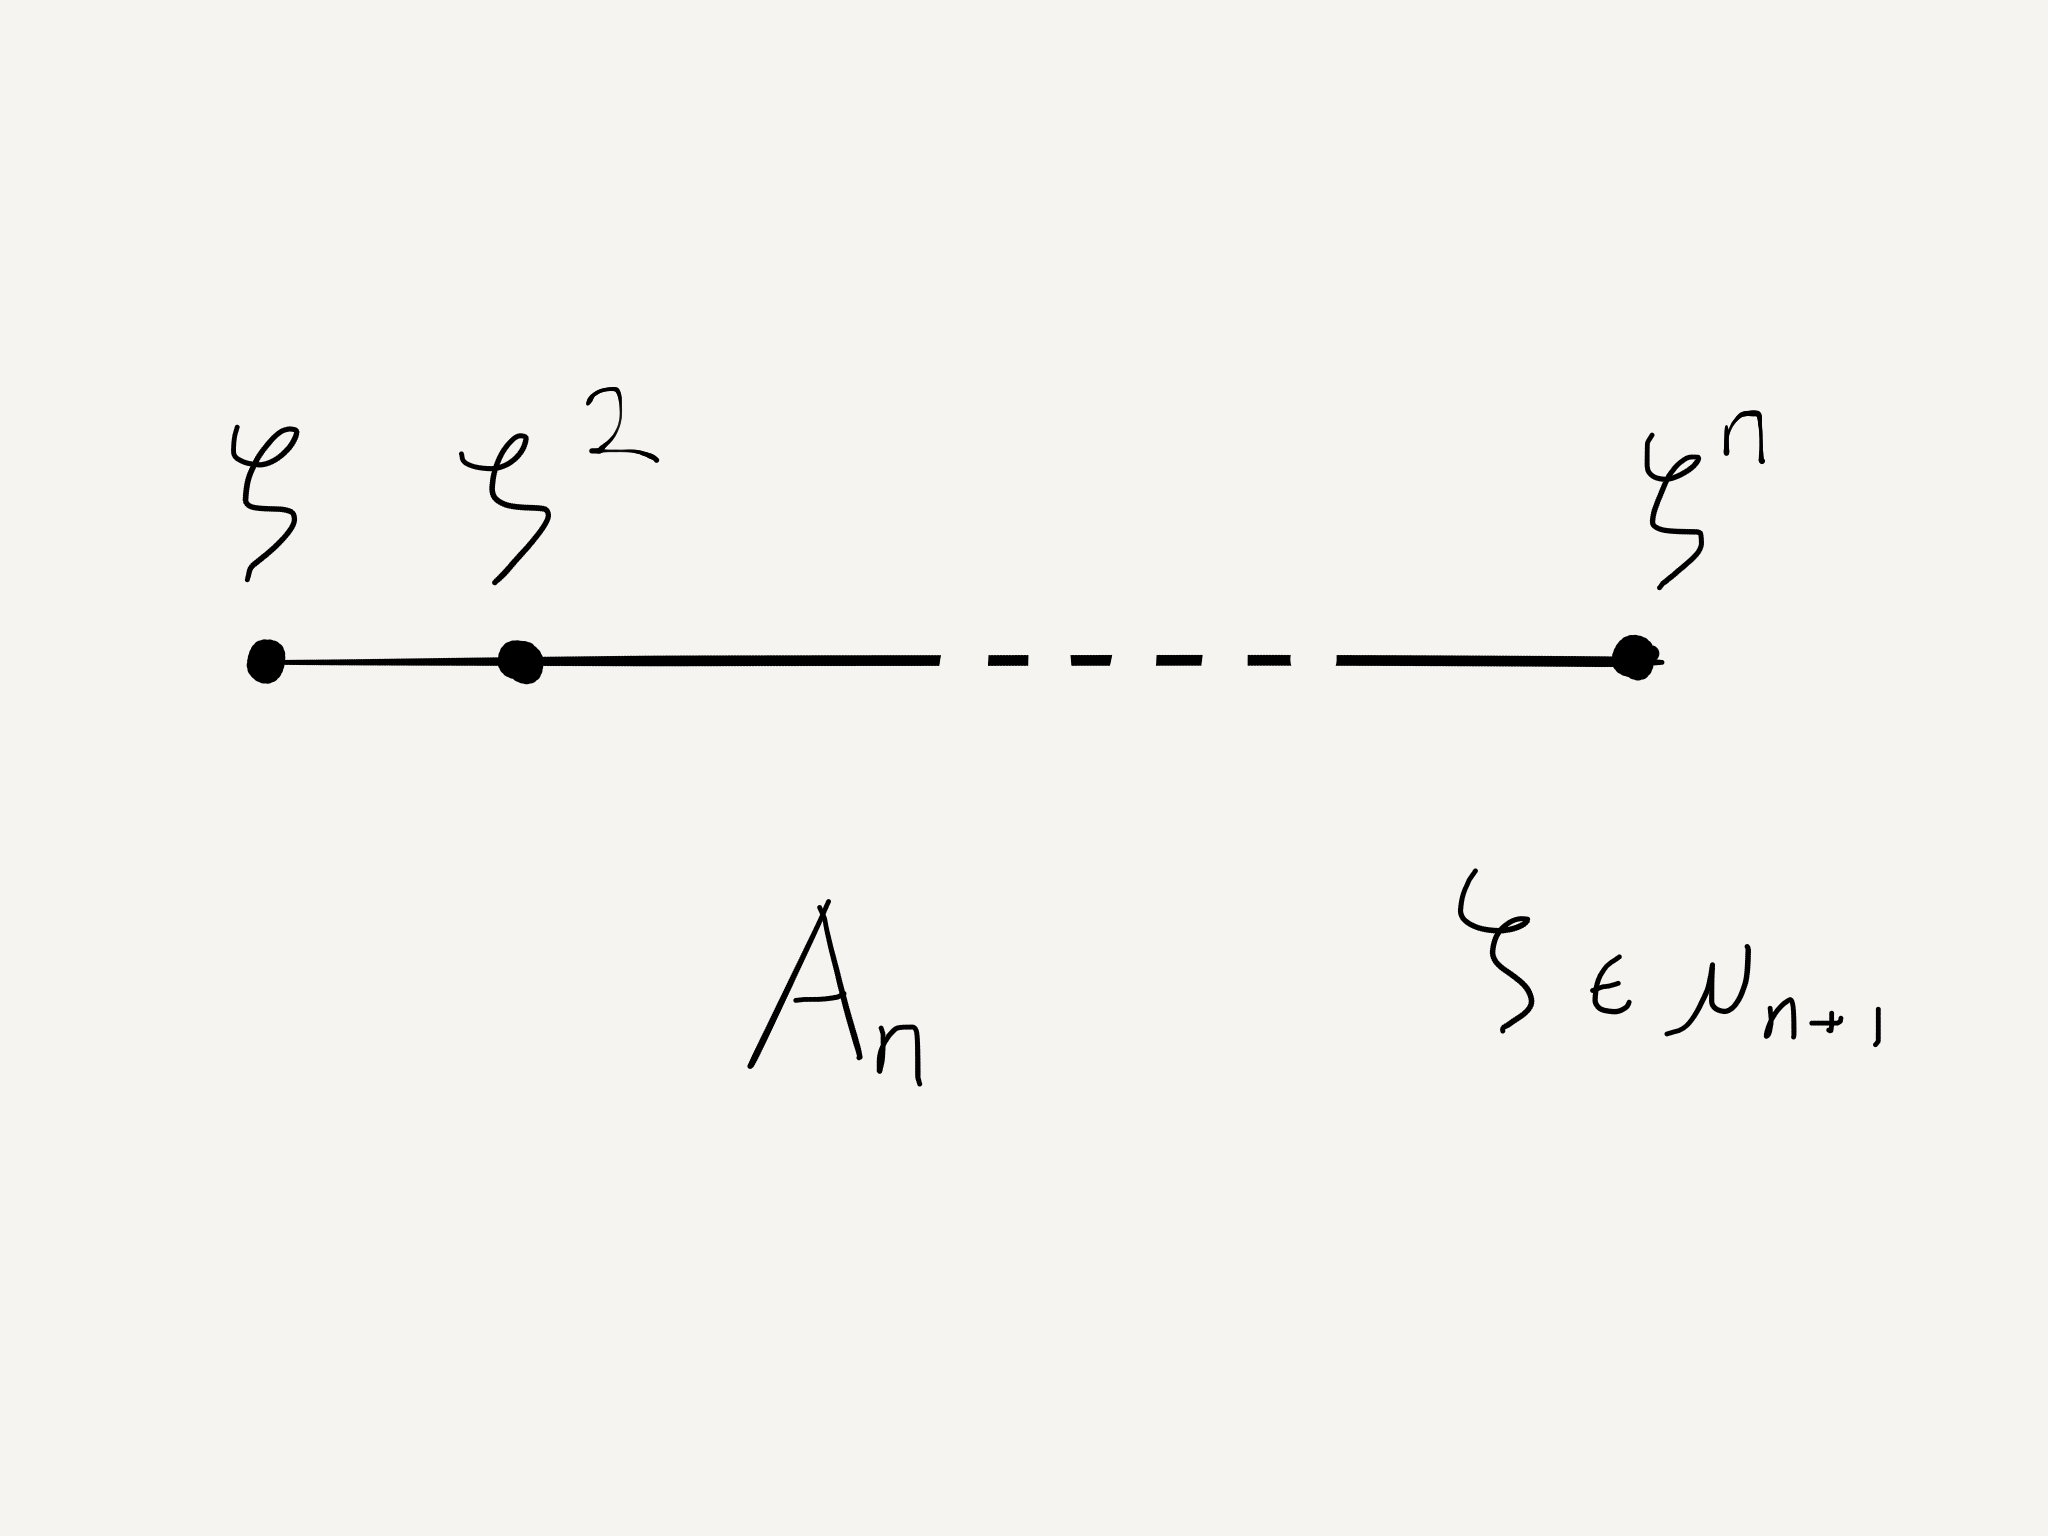
\includegraphics[scale=.15]{249-21.png}
\]

For the additional classical types and exceptional cases E$_6$ and E$_7$ the centers are described as follows:
%\begin{figure}
%\centering
\[
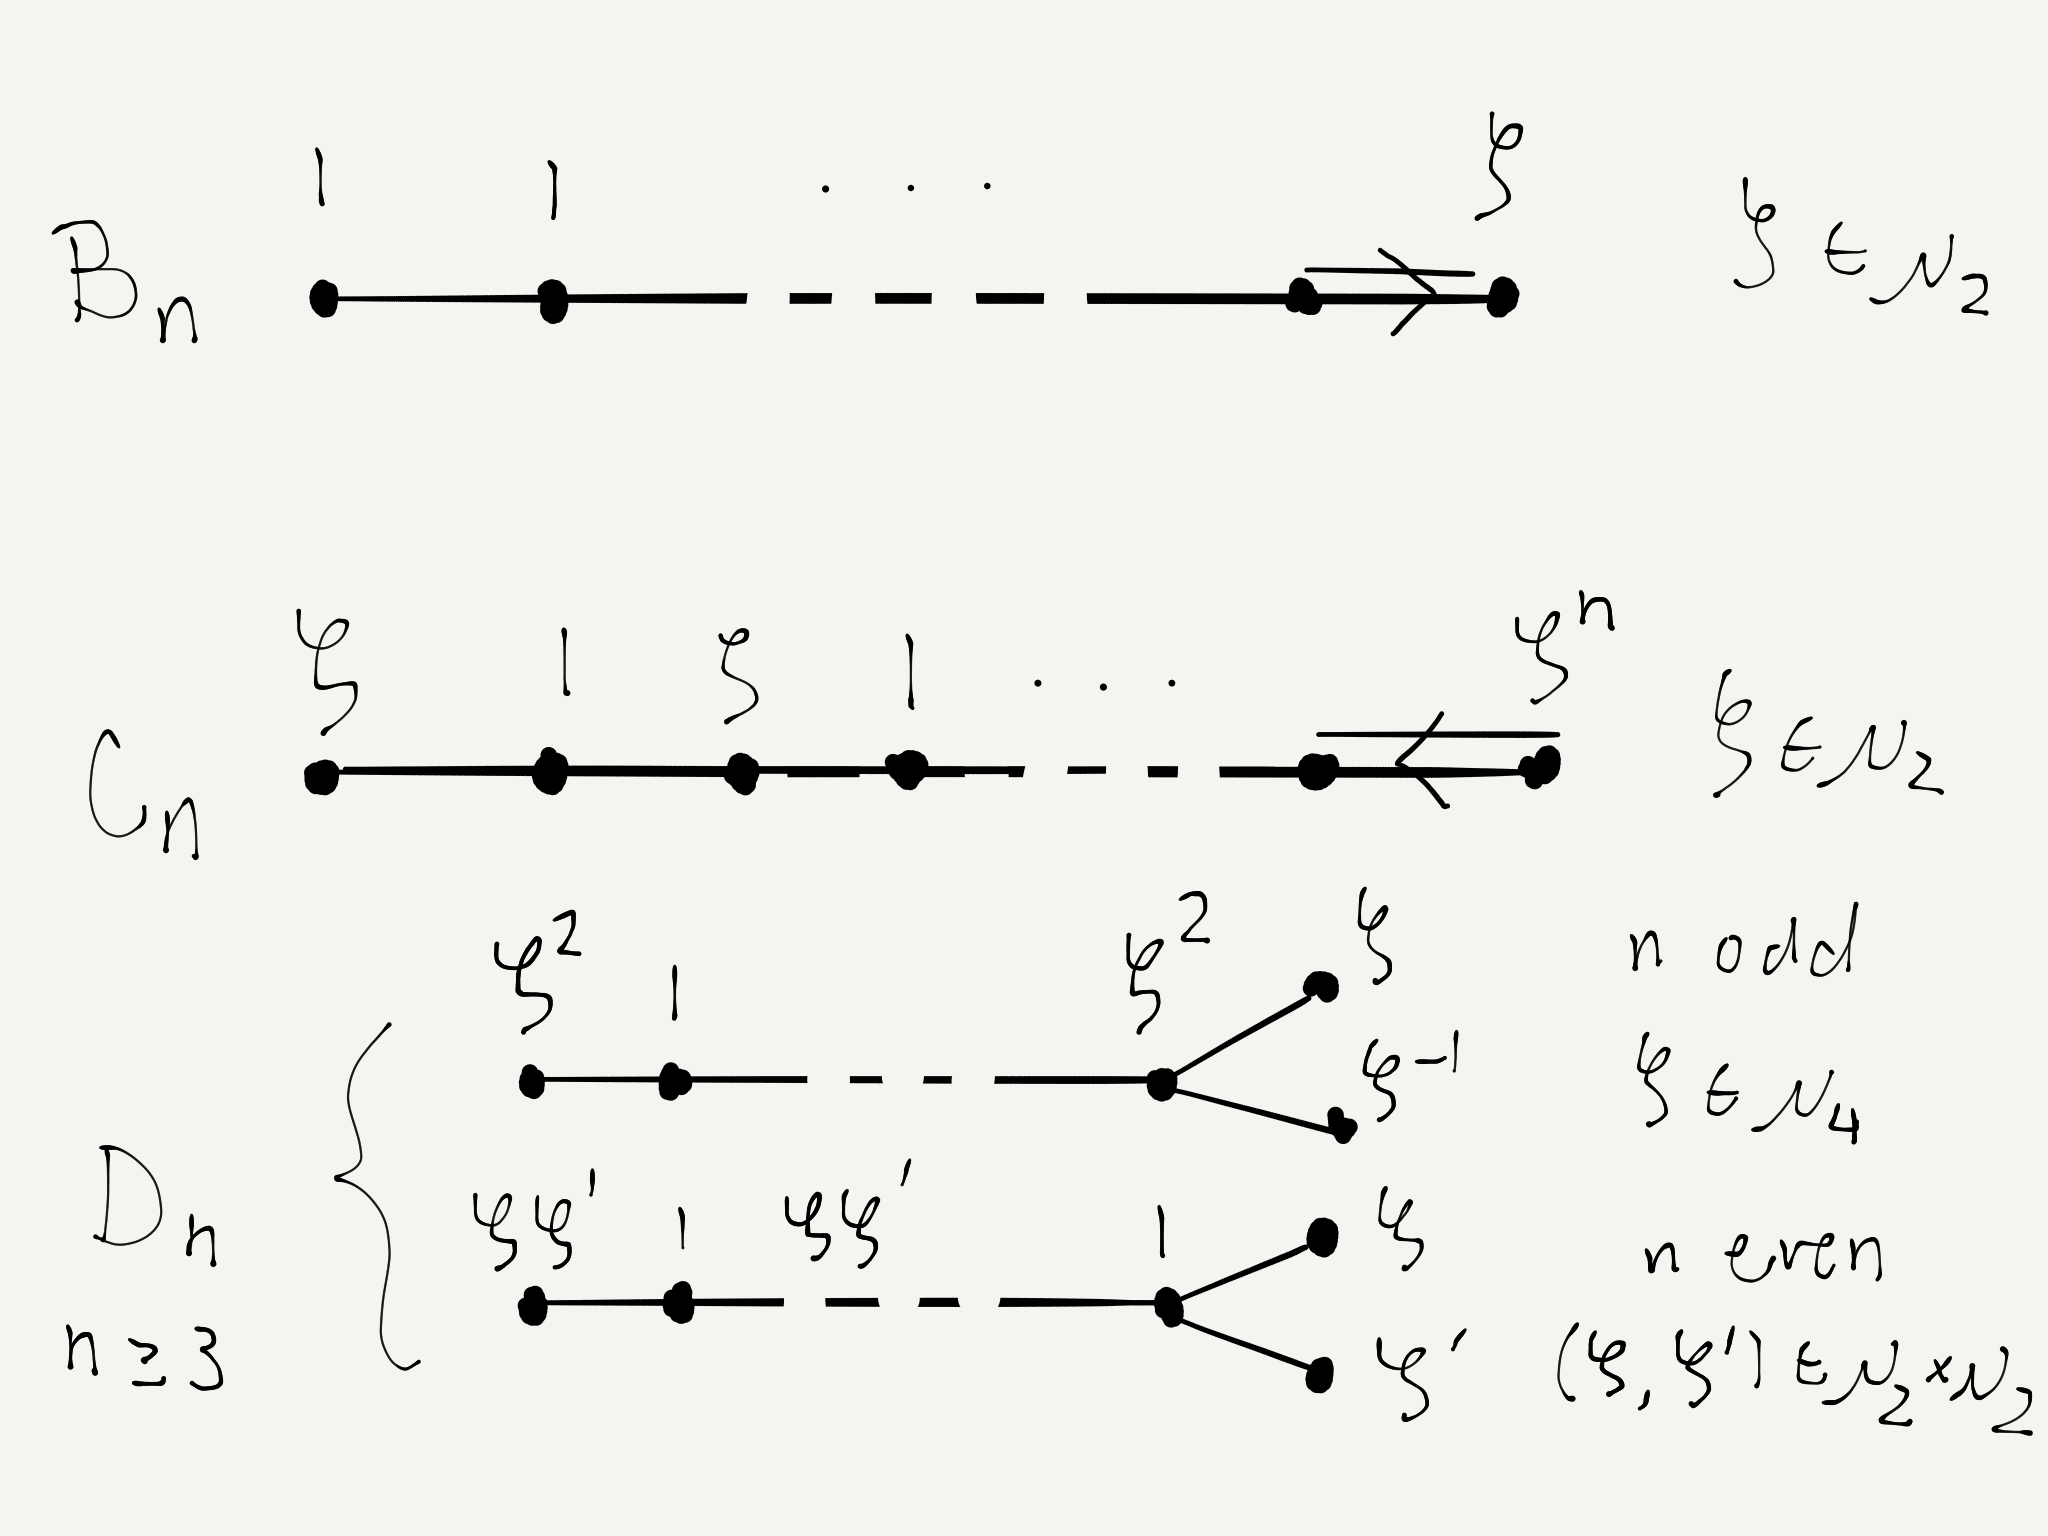
\includegraphics[scale=.2]{249-22.png}
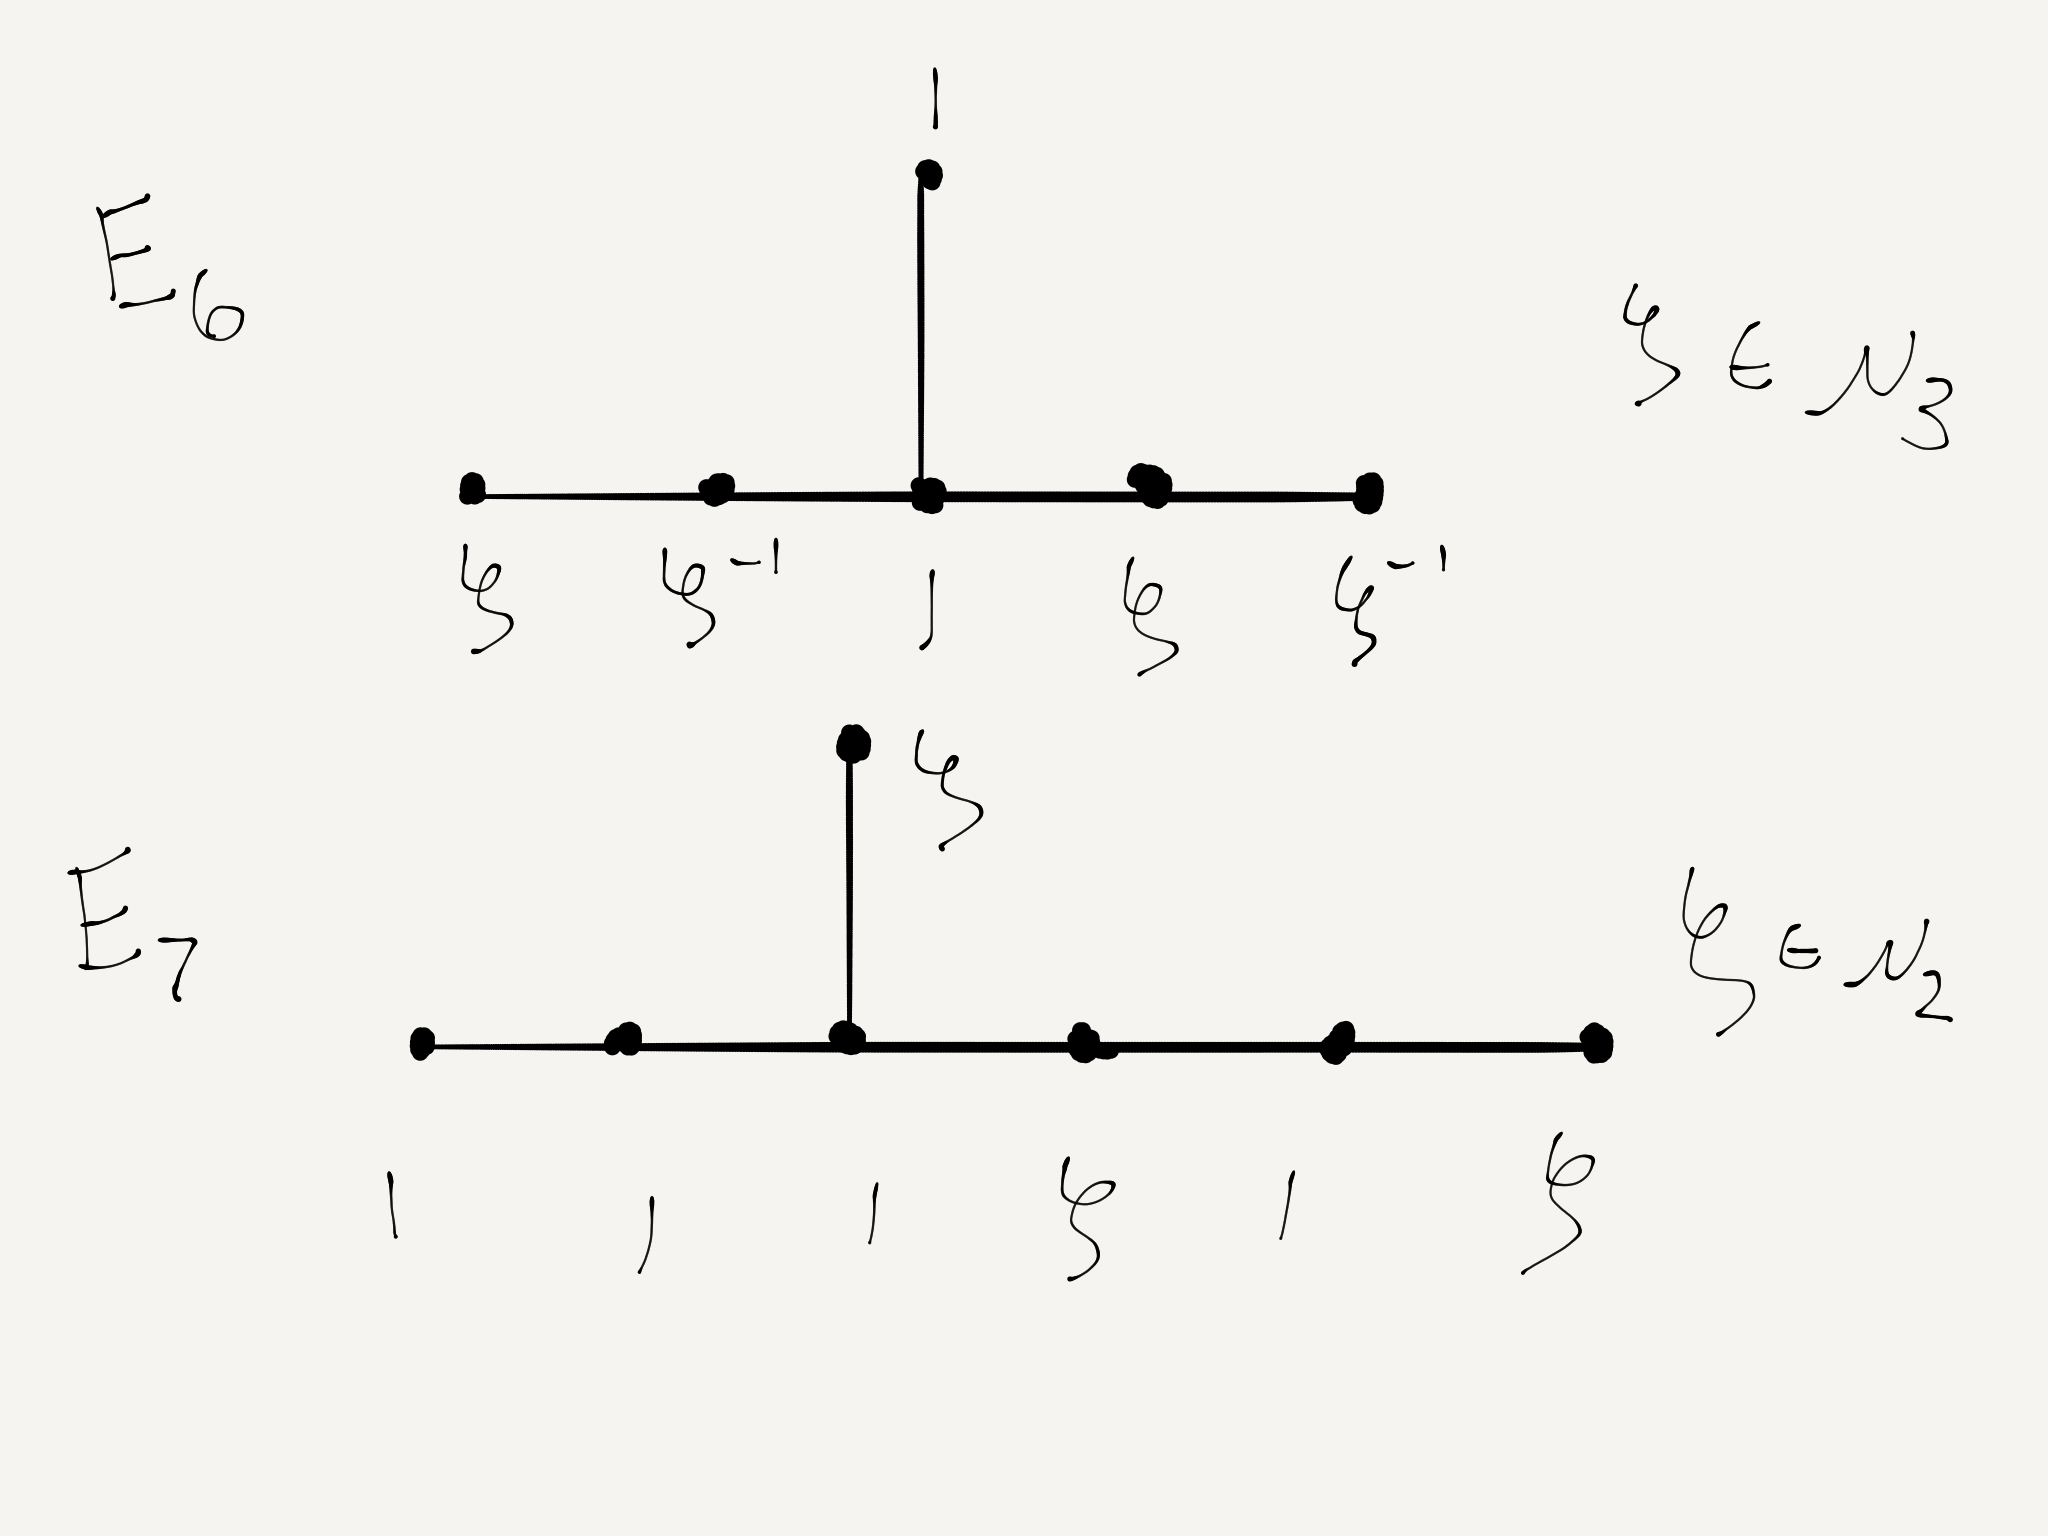
\includegraphics[scale=.2]{249-23.png}
\]
%\caption{Coroot parametrization of center for the remaining connected Dynkin diagrams.}
%\end{figure}
For E$_8$, F$_4$, and G$_2$ the root lattice and weight lattice
coincide, so the center is trivial (i.e., the simply connected group with each of
these root systems is also of adjoint type). 

\begin{remark}
The strongest formulation of
the Isomorphism Theorem gives
an interpretation of diagram automorphisms: these are
the automorphisms of the triple $(G, B, T)$ when $G$ is simply connected,
and the group of such automorphisms maps
isomorphically onto ${\rm{Aut}}_k(G)/(G/Z_G)(k)$. In particular,
as automorphisms these do not arise from the group $G/Z_G$
of ``geometrically inner'' automorphisms.

For example, the evident involution of the A$_{n-1}$-diagram ($n \ge 2$) 
has the effect of inversion on the coroot parameterization of the center $\mu_n$, so an
automorphism of SL$_n$ inducing this could not arise from inner
automorphisms when $n \ge 3$ (as inner automorphisms are always trivial on the center!).
In contrast, ${\rm{Aut}}_k(\SL_2) = \PGL_2(k) = (\SL_2/\mu_2)(k)$, so all automorphisms of $\SL_2$
are geometrically inner. 

Likewise, the involutions of the E$_6$-diagram (with center $\mu_3$)
and the D$_n$-diagram (with center $\mu_4$ or $\mu_2 \times \mu_2$, depending
on the parity of $n$) for $n \ne 4$, as well
as any nontrivial diagram automorphism in the ``triality'' case D$_4$,
 are nontrivial on the coroot parameterizations of their centers by inspection in each case. 
\end{remark}

We now take care of a loose end in our preceding discussion of the classification of reduced root systems,
showing that connectedness of the diagram encodes irreducibility of the root system.

\begin{proposition}\label{conndyn}
Assume that $\Phi$ is reduced. Then $\Dyn(\Phi)$ is connected if and only if $\Phi$ is irreducible. 
\end{proposition}

\begin{proof}
If $\Phi$ is reducible then $\Dyn(\Phi)$ is obviously disconnected. The converse is the hard part. Choose a root basis $\Delta$ for $\Phi^+$. Suppose $\Dyn(\Phi)$ is disconnected; then we can partition $\Delta = \bigsqcup \Delta_i$ via connected components (so each $\Delta_i$ is non-empty and there
are at least two $i$'s). We have 
\[
\Q \Phi= \bigoplus_{a \in \Delta} \Q a = \bigoplus V_i \quad \text{where } V_i = \bigoplus_{a \in \Delta_i} \Q a. 
\]
Let $\Phi_i = \Phi \cap ( \Z \Delta_i) \supset \Delta_i$. Each $(V_i, \Phi_i)$ is a root system, by inspection of the reflection formula 
\[
r_a(b) = b-\langle b, a^{\vee} \rangle a
\]
with $\langle b, a^{\vee} \rangle \in \Z$. 
Also, the roots in $\Delta_i$ are orthogonal to those in $\Delta_j$ for any $j \ne i$ by the meaning of edges
(or lack thereof!) in the diagram.  Clearly $\Delta_i$ is a root basis of $\Phi_i$, so it defines 
a positive system of roots $\Phi_i^+$. We have $\bigsqcup \Phi_i^+ \subset \Phi^+$, and will show
that equality occurs, so taking into account negation would give that $\Phi$ is the direct sum of
the $\Phi_i$'s, contradicting the assumption that $\Phi$ is irreducible. 

So we assume that there exists $a \in \Phi^+$ not in any $\Phi_i^+$ and seek a contradiction. Certainly $a \notin \Delta$, so we can write $a =a' + a'' $ for $a', a'' \in \Phi^+$ (Proposition \ref{sumroot}). 
Choose such an $a$ with minimal total sum of 
$\Delta$-coordinates. By this minimality we must 
have $a' \in \Phi_i^+$ and $a'' \in \Phi_j^+$ for some $i, j$,
and necessarily $i \neq j$ (or else $a$ would be in $\Phi_i^+$). Then 
\[
\Phi \ni r_{a''}(a) = a - \langle a, (a'')^{\vee} \rangle a'' = a' + a'' - \langle a' + a'', (a'')^{\vee} \rangle a''.
\]
Since $a'$ and $a''$ are in distinct components we have $\langle a', (a'')^{\vee} \rangle = 0$. Thus, 
\[
\Phi \ni r_{a''}(a) = a' + a'' - \langle a'', (a'')^{\vee} \rangle a'' = a'-a'',
\]
so we have found a root whose $\Delta$-coordinates of are mixed signs (a positive coordinate
along $\Delta_i$, and a negative coordinate along $\Delta_j$), an absurdity. 
\end{proof}

\end{example}

\section{Structure of reductive groups II}

\subsection{Central isogeny decomposition}

As an application of the theory of root systems, we are ready to prove Theorem \ref{ss_decomp}, reproduced below. 


\begin{theorem}\label{gnormal}
Let $G$ be a connected semisimple $k$-group $G$,
and $\{G_i\}$ its set of minimal non-trivial smooth connected normal 
$k$-subgroups $($all semisimple by normality, since for any smooth connected
normal $k$-subgroup $N \subset G$ the solvable radical of $N_{\overline{k}}$ 
 is stable under all $G(\overline{k})$-conjugations and hence
is contained in $\Cal{R}_u(G_{\overline{k}}) = 1$).  The following hold: 
\begin{enumerate}
\item the set $\{G_i\}$ is finite and these pairwise commute, with 
the multiplication homomorphism $\prod G_i \rightarrow G$ a central $k$-isogeny; 
\item each $G_i$ is $k$-simple;
\item the smooth connected normal $k$-subgroups of $G$ are exactly 
\[
N_J = \langle G_i \rangle_{i \in J}
\]
for subsets $J \subset I$. Moreover,
$N_J \subset N_{J'}$ if and only if $J \subset J'$
$($so $G_i \subset N_J$ if and only if $i \in J)$.
\end{enumerate}
\end{theorem}

To provide more motivation, first we shall deduce 
two striking corollaries and then we will take up the proof of the theorem.

\begin{lemma} Let $G$ be a connected reductive group over a field $k$,
and let $N$ be a smooth connected normal $k$-subgroup of $G$.
\begin{itemize}
\item[(i)] If $N'$ is a smooth connected
normal $k$-subgroup of $N$ then $N'$ is normal in $G$.
\item[(ii)] If $G$ is semisimple then there is a unique smooth connected normal $k$-subgroup
$\mathscr{N} \subset G$ commuting with $N$ such that the natural
homomorphism $N \times \mathscr{N} \rightarrow G$ is an isogeny $($in fact, it is a central isogeny$)$.
\end{itemize}
\end{lemma}

\begin{proof}  First consider connected semisimple $G$.  By Theorem \ref{ss_decomp}, 
we have $N = \langle G_i\rangle_{i \in J}$ for a unique subset $J \subset I$.
The multiplication map $\prod_{i \in J} G_i \rightarrow N$
is surjective and it has finite central kernel since even $\prod_{i \in I} G_i \rightarrow G$ has finite central kernel.
In particular, $\sum_{i \in J} \dim G_i = \dim N$. 
The $G_i$'s for $i \in J$ are certainly minimal nontrivial smooth connected normal $k$-subgroups of $N$
(as they are minimal as such in $G$), and Theorem \ref{ss_decomp} applied to $N$
implies by dimension considerations that there are no others.  Hence, $\{G_i\}_{i \in J}$
is the output of Theorem \ref{ss_decomp} applied to $N$.  

In the setting of (i) for semisimple $G$, we can apply the same conclusion with $N'$ in the role of $N$
and with $N$ in the role of $G$, so $N'$ must be generated by $G_i$'s for $i$ varying through
some subset of $J$.  This implies that $N'$ is normal in $G$, so (i) is proved when $G$ is semisimple.

In general, if $G$ is reductive then $G$ is a central isogenous quotient of its maximal
central $k$-torus $Z$ and its semisimple derived group $\mathscr{D}(G)$.
Likewise, $N$ inherits reductivity from $G$ (as we may
check over $\overline{k}$), so it is a central isogenous quotient of its maximal central $k$-torus
$S$ and its semisimple derived group $\mathscr{D}(N)$. 
By normality of $N$ in $G$ and the compatibility of the formation of $S$
with respect to any extension of the ground field it follows that the torus $S$ inherits
normality in $G$ from that of $N$.  Thus, the torus $S$ must be central in $G$ (as $G$ is connected),
so $S \subset Z$.
Likewise $N'$ is a commuting quotient of its maximal central torus $S'$ that must be contained
in $S$ (so $S' \subset Z$) and its semisimple derived group $\mathscr{D}(N')$. 
Since $\mathscr{D}(N)$ is normal in $\mathscr{D}(G)$ (due to normality of $N$ in $G$)
and $\mathscr{D}(N')$ is likewise normal in $\mathscr{D}(N)$, the settled
semisimple case implies that $\mathscr{D}(N')$ is normal in $\mathscr{D}(G)$.
But $G = Z \cdot \mathscr{D}(G)$ with $Z$ central, and $S' \subset Z$, so
$N' = S' \mathscr{D}(N')$ is normal in $G$ as desired.  This proves (i) in general. 

In the setting of (ii), our description of the possibilities for $N$ 
applies to any possibility for $\mathscr{N}$, so it follows
that the only possibility for $\mathscr{N}$ is $\langle G_i \rangle_{i \in I - J}$
and this clearly does work (and gives a central isogeny since $\prod_{i \in I} G_i \rightarrow G$
is a central isogeny).   This proves (ii).
\end{proof}

For connected semisimple
$G$, the $k$-subgroups $G_i \subset G$ are called the {\em $k$-simple factors} of $G$. In general
these are not direct factors, but in two important cases they are:

\begin{lemma}\label{scadisom} If $G$ is connected semisimple then the central isogeny
$f:\prod G_i \rightarrow G$ is an isomorphism if $G$ is either simply connected or of adjoint type
$($in which case each $G_i$ inherits the same property$)$.
\end{lemma}

\begin{proof}
If $G$ is simply connected then we know that there is no nontrivial central
isogeny onto $G$ from another connected semisimple group.
This settles the simply connected case.  

Suppose instead that $Z_G=1$.
To prove $f$ is an isomorphism, by the centrality of $\ker f$
note that $\ker f \subset \prod Z_{G_i}$. Hence, to prove $\ker f = 1$ (so $f$ is an isomorphism)
it suffices to directly prove that $Z_{G_i} = 1$ for each $i$. 
But $G_i$ commutes with $G_j$ for all $j \ne i$, so $Z_{G_i}$ commutes with $G_j$ for {\em all} $j$.
The faithful flatness of $\prod_{j \in I} G_j \rightarrow G$ then implies
that $Z_{G_i}$ centralizes $G$, so $Z_{G_i} \subset Z_G = 1$ as desired. 
\end{proof}

\begin{remark}
The significance of Corollary \ref{scadisom} is addressed in Appendix \ref{simplefactor}
in both the simply connected and adjoint-type cases, to each class of which any connected semisimple
$k$-group is canonically related via a central $k$-isogeny, the group
$G$ admits an isomorphism to ${\rm{R}}_{k'/k}(G')$ for a {\em canonically associated}
pair $(k'/k, G')$ consisting of a finite \'etale $k$-algebra $k'$
and a smooth affine $k'$-group $G'$ whose fiber $G'_i$ over each factor
field $k'$ of $k$ is a connected semisimple $k_i$-group that is {\em absolutely simple}.

This explains the essential role of the absolutely simple case (over finite separable extensions
of $k$) in the study of general connected semisimple groups over $k$.  More specifically,
constructions as in Example \ref{weilks} (but without
the split hypothesis imposed there) are more ubiquitous than one might have initially expected.
\end{remark}

\subsection{Proof of Theorem \ref{ss_decomp}}

The general case can be deduced from the split case; this is explained in Appendix \ref{simplefactor}
via arguments with Galois descent.   
Here we will focus on the split case, so suppose $G$ admits a split
maximal $k$-torus $T \subset G$.
The key tool in the proof is the irreducible decomposition of root systems. 

The idea is to 
build the $G_i$'s directly from the irreducible components $\Phi_i$ of $\Phi(G, T)$,
and they will be $k$-split with root system $\Phi_i$.  Thus, the $k$-simplicity of each $G_i$
will reduce to proving the general fact that when $\Phi$ is irreducible then $G$ is $k$-simple
(and so absolutely simple, since $\Phi$ never changes under field extension in the split case). 
Such $k$-simplicity will ultimately rest on a nontrivial fact in the theory of
root systems: if $(V, \Phi)$ is an irreducible root system then $W(\Phi)$ acts irreducibly (even absolutely irreducibly)
on $V$.

Let $\Phi = \Phi(G, T)$, and $V = X_{\Q}$ for $X = {\rm{X}}(T)$, so $V$ is spanned by $\Phi$ (as $G$
is semisimple).  Let $\Delta$ be the base for a positive system of roots $\Phi^+ \subset \Phi$,
and consider the irreducible decomposition
$$(V, \Phi) = \bigoplus_{i \in I} (V_i, \Phi_i),$$
under which $\Delta$ decomposes as $\coprod \Delta_i$ for a base $\Delta_i$
of $\Phi_i^+ = \Phi_i \cap \Phi^+$.


We want to define $G_i = \langle U_a \rangle_{a \in \Phi_i}$. The problem is that it is hard to prove much using this definition, so we're going to take a different approach, using torus centralizers and various commutators instead. Informally, we want $\prod G_i \rightarrow G$ to be a central isogeny, so we know that the tori should match up: 
\[
\xymatrix@C=0pc{
\prod G_i \ar[d] &\supset  & \prod T_i \ar@{->>}[d] \\
G &\supset & T
}
\]
We'll first build the $T_i$'s and define $G_i = \Cal{D}(Z_G(T_i'))$ where $T_i' = \langle T_j \rangle_{j \neq i}$. 

One could try to define these tori $T_i \subset T$ using quotients
of $X$, but this leads to confusion because the character lattice is contravariant
(and may lead to some mild headaches since $X/\sum_{j \ne i} \Z \Psi_j$ may have
nonzero torsion. Hence,
it is more useful to use \emph{cocharacters}, so we'll build $T_i \subset T$ using coroots for $\Phi_i$. 

Consider the isogeny
\begin{align*}
\G_m^{\Delta} & \rightarrow T \\
(y_a) & \mapsto  \prod a^{\vee}(y_a)
\end{align*}
Letting $T_i = \Ima(\G_m^{\Delta_i} \rightarrow T)$, we have a factorization 
\[
\G_m^{\Delta} \twoheadrightarrow \prod T_i \twoheadrightarrow T
\]
of an isogeny into a composition of surjections, so the second map
$\prod T_i \rightarrow T$ induced by multiplication
must be an isogeny, with ${\rm{X}}_*(T_i)_{\Q} = \Q  \Delta_i^{\vee} = \Q \Phi_i^{\vee}$. 

Define $T_i' = \langle T_j \rangle_{j \neq i} \subset T$, so 
\[
T_i' \times T_i \rightarrow T
\]
is an isogeny. Set $G_i = \Cal{D}(Z_G(T_i'))$. It is not yet clear that $T_i \subset G_i$, nor
that $T'_i$ is the maximal central torus in $Z_G(T'_i)$ (in general, a torus need not be the maximal torus in its centralizer: this fails for
the centralizer of a maximal split torus in any quasi-split group that is not split). 

The roots of $G_i = \Cal{D}(Z_G(T_i'))$ relative to its {\em split} maximal torus intersection with
$T$ are the same as the $T$-roots of $Z_G(T_i')$. (Note that $G_i$ is normalized by $T$, since it is a characteristic subgroup of $Z_G(T_i) \supset T$.) The $T$-roots for $Z_G(T_i')$ are the $T$-roots for $G$ 
that are \emph{trivial} on $T_i' = \langle T_j \rangle_{j \neq }$, so the $T$-roots for $Z_G(T_i')$ are exactly the roots $a \in \Phi$ such that $\langle a, b^{\vee} \rangle = 0$ for all $b  \in \coprod_{j \neq i} \Phi_j $. 
Via the decomposition $X_{\Q} = {\rm{X}}(T'_i)_{\Q} \oplus {\rm{X}}(T_i)_{\Q}$
we have shows that $\Phi_i \subset {\rm{X}}(T_i)_{\Q}$, so ${\rm{X}}(T_i)_{\Q} \supset \Q \Phi_i = V_i$.
Passing to the direct sum over all $i$ yields an equality, so ${\rm{X}}(T_i)_{\Q} = V_i$
inside $X_{\Q} = V$.  

It is clear from the irreducible decomposition that the set of such $a$ is exactly $\Phi_i$.
Hence, the $T$-root groups for $Z_G(T_i)$ are the $U_a$'s for $a \in \Phi_i$
(in view of the unique characterization for root groups, those of $Z_G(T_i)$ and $G$
for a common $T$-root must coincide).  Thus, the split derived group $G_i$ is generated by 
the $U_a$'s for $a \in \Phi_i$, and its associated coroots must coincide
with those for $(G, T)$ relative to $a$ (as each is determined by $\langle U_a, U_{-a} \rangle$
and its intersection with $T$).   It follows that $G_i$ contains
$\langle a^{\vee}(\mathbf{G}_m) \rangle_{a \in \Phi_i} = T_i$, and as such $T_i$ must be
a split {\em maximal} torus of $G_i$.  By dimension reasons with tori, it follows that $T'_i$
must exhaust the maximal central torus in $Z_G(T'_i)$. 

\begin{lemma}
If $i \neq j$ then $G_i$ commutes with $G_j$.
\end{lemma}

\begin{proof}
It is enough to show that $[U_a, U_b] = 1$ for $a \in \Phi_i$ and $b \in \Phi_j$. We can pick $\Phi^+$ such that $a \in \Phi_i^+$ and $b \in \Phi_j^+$. Then 
\[
(U_a, U_b) \subset \prod_{c \in (a,b)} U_c 
\]
where $(a,b) = \Phi \cap (\Z_{>0} a + \Z_{>0} b) = \emptyset$ because $\Phi = \coprod \Phi_i \subset \bigoplus V_i$. 
\end{proof}

This shows that we have a multiplication homomorphism 
\[
\xymatrix@C=0pc{
\prod G_i  \ar@{->>}[d]_f &\supset & \prod T_i \ar@{->>}[d] \\
G &\supset & T 
}
\]
so $(\ker f_{\ol{k}})^0_{\red}$ has no non-trivial torus, hence is trivial (because it is normal in a reductive group). Therefore, $\ker f$ is finite; i.e. $f$ is an isogeny. 


\begin{lemma}
The subgroup scheme $\ker f \subset \prod G_i$ is central.
\end{lemma}

\begin{proof}
For a $k$-algebra $R$, consider $(g_i) \in (\ker f)(R)$ so $g_i^{-1} = \prod_{j \neq i} g_j$ inside $G(R)$. Then $g_i$ commutes with $(G_i)_R$  (as each
$(G_j)_R$ does) and also with $(G_j)_R$ for all $j \neq i$, so by the faithful flatness of $\prod_{i' \in I} G_{i'} \twoheadrightarrow G$, we have $g_i \in Z_G(R)$. 
\end{proof}

It remains to show:

\begin{proposition}
We have:
\begin{enumerate}
\item each $G_i$ is $k$-simple $($even absolutely simple$)$,
\item each smooth connected $N \triangleleft G$ is of the form $\langle G_i \rangle_{i \in J}$ for $J = \{i \in I \mid G_i \subset N\}$, and $N \cap G_i $ is finite for all $i \notin J$.
\end{enumerate}
\end{proposition}

\begin{remark}
The second part implies that the $G_i$ are the minimal nontrivial smooth connected normal $k$-subgroups
(as we wanted them to be).  This finally provides a description of the $G_i$ that doesn't mention $T$!
\end{remark}

\begin{proof}
Let's first show that $(1) \implies (2)$. Choose $N \subset G$ as in (2), with $N \neq 1$
without loss of generality. It suffices to show that some $G_i \subset N$, since we can then induct, by passing to the quotient $G/G_i \triangleright N/G_i$ with minimal normal subgroups $\overline{G}_j :=
G_j/G_j \cap G_i$ (central isogenous quotients of $G_j$, hence with the {\em same}
root system as $G_j$ relative to the image of $T_j$).  The main point, left to the reader to check by
going back to the definitions, is that $\Phi(G/G_i, T/T_i) = 
\coprod_{j \ne i} \Phi_j$ and that $\{\overline{G}_j\}_{j \ne i}$ is 
the output of our main construction applied to $G/G_i$ relative to its split maximal $k$-torus $T/T_i$.

Now we find some $G_i$ contained in $N$, granting (1). 
Certainly $N$ is not central in $G$ since $Z_G$ is finite and the smooth connected $N$
is nontrivial, so there exists some $G_{i_0}$ which doesn't commute with $N$. Consider $[G_{i_0},N]$, which is non-trivial by assumption.  It is a smooth connected normal subgroup of $G$, and it is contained in both $N$ and $G_{i_0}$ by the normality of each in $G$. By (1), the containment $[N, G_{i_0}] \subseteq G_{i_0}$ is 
therefore an equality, so $G_{i_0} = [N, G_{i_0}] \subset N$. 

It remains to show (1). Renaming $G_i$ as $G$, we reduce to the following lemma.
\end{proof}

\begin{lemma}
If $\Phi$ is irreducible then $G$ is absolutely simple over $k$. 
\end{lemma}

\begin{proof}
Without loss of generality assume $k =\ol{k}$. Consider $N \triangleleft G$ a nontrivial smooth connected normal $k$-subgroup. Note that $\Cal{R}(N)$ is solvable connected normal in $G$, which is connected semisimple, so $\Cal{R}(N)=1$; i.e. $N$ is also semisimple. 

The goal is to show that $N=G$. We'll do this by showing that a maximal torus for $N$ is one for $G$ as well. This will conclude the proof, because then 
the maximal torus image of $T$ in
the connected semisimple group $G/N$ is trivial, forcing $G/N = 1$; i.e., $N = G$.

Pick a maximal torus $S \subset N$ (so $S \ne 1$, since
$N \ne 1$) and extend it to a maximal torus $T \subset G$; note that $S \subset T \cap N \subset Z_S(N) = S$ so $T \cap N = S$. Thus, $N_G(T)(k)$-conjugation preserves $T \cap N = S$, and so 
$N_G(T)(k)$ naturally acts on ${\rm{X}}(S)$.  The quotient map
\[
{\rm{X}}(T)_{\Q} \twoheadrightarrow {\rm{X}}(S)_{\Q} \ne 0.
\]
is clearly equivariant for the natural action of $W(G, T) = W(\Phi)$ on ${\rm{X}}(T)_{\Q}$.
But as a representation space for $W(\Phi)$, 
we know that ${\rm{X}}(T)_{\Q}$ is (absolutely) irreducible since $\Phi$ is irreducible (Proposition \ref{abs_irr_root}), 
so this forces $S=T$. 
\end{proof}

\subsection{Bruhat decomposition}
Let $G$ be a connected reductive group over $k$,  $S \subset G$ a maximal split $k$-torus, and $P \subset G$ a minimal parabolic $k$-subgroup such that $S \subset P$. Then $N := N_G(S) \supset Z_G(S) =: Z$ and $P = Z \ltimes U$ for $U = \Cal{R}_{u,k}(P)$, which is $k$-split
(as the smooth connected unipotent $k$-groups $U_G(\lambda)$ built
by the dynamic method for smooth connected affine $G$ and nontrivial cocharacters $\lambda$ 
are always $k$-split). 
We consider the relative Weyl group $_k W := N(k)/Z(k)$ that is always a finite group
(being contained in $(N/Z)(k)$ with $N/Z$ a finite type $k$-subgroup of the \'etale
automorphism scheme of $S$).

We want to show:
\begin{theorem}[Relative Bruhat decomposition]\label{rel_bruhat} We have that 
\begin{enumerate}
\item the natural map $_k W \rightarrow  P(k) \backslash G(k) / P(k)$ is bijective, 
\item the finite $k$-group $N/Z$ is constant and the natural map $N(k)/Z(k) \rightarrow (N/Z)(k)$
is bijective. 
\end{enumerate}
\end{theorem}


\begin{remark}\label{relrem}
The relative Bruhat decomposition is not a ``geometric'' result: this 
equality at the level of rational points does not correspond to
 a stratification of $G$ \emph{except} in the split case. However, we make the following remarks.
\begin{enumerate}
\item[(i)] In (1) one has the stronger disjointness
property that the locally closed subvarieties $\{Pn_wP\}_{w \in {}_kW}$ inside $G$ \emph{are} pairwise disjoint;
this is proved in \S3 of Appendix \ref{relbruhat}. 
\item[(ii)] The constancy of $N/Z$ in (2) is easy: this finite type $k$-group scheme
is a $k$-subgroup of the \'etale (locally finite type) automorphism scheme ${\rm{Aut}}_{S/k}$ that is constant
since $S$ is split (it is represented by ${\rm{GL}}_n(\Z)$ if $S \simeq \G_m^n$).  

But the equality in (2)
is less clear. The proof uses 
that $N_G(S) \cap P = Z_G(S)$ to show that $N(k)/Z(k)$ and $(N/Z)(k)$
compatibly act simply transitively on the 
set of minimal parabolic $k$-subgroups of $G$ containing $S$. (Note the analogy with our proof of 
such an equality in the split case, though at present we have not yet proved
that $\Phi(G, S)$ is a root system inside its $\Q$-span in ${\rm{X}}(S)_{\Q}$.)  This argument
is given in \S4 of Appendix \ref{relbruhat}. 
\item[(iii)] In the split case (2) is immediate from Hilbert 90 (since $Z$ is a split torus in such cases), but
its validity beyond the split case is remarkable because often ${\rm{H}}^1(k, Z) \neq 1$ when $G$ is not split.
Two classes of examples with non-split quasi-split $G$ (so $Z$ even a torus), including
some absolutely simple cases, are given
in \S5--\S7 of Appendix \ref{relbruhat}. 
\end{enumerate}
\end{remark}


The proof of the Bruhat decomposition in the general case involves passage to problems over $\ol{k}$
that are solved using the Bruhat decomposition over $\ol{k}$ (with Borel subgroup).
Hence, we'll treat the split case first (aside from some gritty group-theoretic calculations 
that are presented in full in Appendix \ref{bruhat}), and then turn to the general case. 


\begin{proof}[Proof of split case]
Now assume that $S$ is a maximal $k$-torus of $G$, so we denote
it as $T$. Let $\Phi = \Phi(G,T)$ and $W := W(\Phi) = N(k)/Z(k)$. For $w \in W$, let $n_w \in N(k)$ be a representative (the choice of which will be easily seen not to matter in what follows).
Let $\Phi^+ = \Phi(B, T)$, and let $\Delta$ be the corresponding root basis.
 We need to show that the $B(k)$-double cosets 
 $B(k) n_w B(k)$ for $w \in W$ (which clearly do not depend on the choice of $n_w$) 
 form a pairwise disjoint cover of $G(k)$. 
 Note that for disjointness it is enough to check over $\ol{k}$.

Define $C(w) = Bn_w B$, the $B \times B$-orbit of $n_w$ in $G$ under the action $(b,b').g = bg{b'}^{-1}$,
so $C(w)$ is naturally a smooth locally closed subvariety of $G$. 
We call $C(w)$ the \emph{Bruhat cell} for $w$. It suffices to prove:
\begin{enumerate}
\item[(i)] the $C(w)$'s are pairwise disjoint (as locally closed subschemes of $G$), 
\item[(ii)] the subschemes $C(w)$ cover $G$ (which is sufficient to check on $\ol{k}$-points, as each $C(w)$ is locally
closed), so $G(k)$ is the disjoint union of its subsets $\{C(w)(k)\}_{w \in W}$, 
\item[(iii)] the natural inclusion $B(k)n_w B(k) \subset C(w)(k)$ is an equality. 
\end{enumerate}

We first dispose of (iii) using the product structure of open cells for $G$ relative to 
the borus $(B, T)$. The point is to remove as much of the redundancy  as possible in the description
of points in $BnB$ by moving parts of the left $B$ into the right one. Recall that 
 \[
 B = T \ltimes U
 \]
 for $U := \mathscr{R}_{u,k}(B) = \prod_{a \in \Phi^+} U_a$, with multiplication
 of the positive root groups taken in \emph{any} order (Theorem \ref{3311}). Since $n_w$ normalizes $T$, we have. 
 \[
 B(k)n_wB(k) = U(k)n_wB(k)
 \]
Next observe that $U_a n_w = n_w U_{w^{-1}(a)}$ for any $a \in \Phi$, 
so if $w^{-1}(a)$ is positive then we can move it across as well.  This motivates us to define
 \begin{align*}
 \Phi_w^+ &= \{ a \in \Phi^+ \mid w^{-1}(a) \in \Phi^+\} \\
 \Phi'_w &= \{ a \in  \Phi^+ \mid w^{-1}(a) \in -\Phi^+\}
 \end{align*}
 (We write $\Phi'_w$ rather than $\Phi^{-}_w$ to avoid notational confusion: one can make the analogue
 of $\Phi^+_w$ for $\Phi^{-} := -\Phi^+$ in place of $\Phi^+$, but this does not agree with
$\Phi'_w$.) 
 These are \emph{closed} subsets of $\Phi^+$, so by Theorem \ref{3311}
 we have smooth connected
 $k$-subgroups $U_{\Phi'_w}, U_{\Phi_w^+} \subset U$ 
 that are respectively \emph{directly spanned} (in any order) by the root groups for 
 $\Phi'_w, \Phi_w^+$. 
 
Clearly we have  $U = U_{\Phi'_w} \times U_{\Phi_w^+}$ via multiplication, so 
 \[
 B(k) n_w B(k) = U_{\Phi'_w}(k)  n_w B(k).
 \]
 This has \emph{all} redundancy removed, by applying the following proposition on $k$-points.
 
 \begin{proposition}\label{unb}
The multiplication map 
\[
U_{\Phi'_w}  n_w \times  B \rightarrow C(w)
\]
is an isomorphism of $k$-schemes.
 \end{proposition}
 
This implies that $C(w)/B \simeq U_{\Phi'_w} n_w \simeq \A_k^{\# \Phi'_w}$ is an \emph{affine space},
so the Bruhat decomposition thereby provides
a covering of $G/B$ by affine spaces.   
A result in the theory of root systems (see Remark \ref{longw} for the Bourbaki reference) gives that
$\# \Phi'_w$ coincides with the minimal length $\ell(w)$ of $w$ as a word
in the generating set $\{r_a\}_{a \in \Delta}$ of the Coxeter group $W$.

\begin{proof}
Running the preceding calculation on $k$-points with $\ol{k}$ in place of $k$ gives
an equality
\[
C(w) = Bn_w B = U_{\Phi'_w}n_w B
\]
of smooth locally closed subschemes of $G$ (as such an equality holds
if it does on $\ol{k}$-points), so it suffices to show that the multiplication morphism
\[
U_{\Phi'_w} n_w \times B \rightarrow G
\]
(whose image is $C(w)$) is a locally closed immersion. 

It is harmless to first
apply left multiplication by $n_w^{-1}$, which turns this into the multiplication map
\[
U_{w^{-1}(\Phi'_w)} \times B \xrightarrow{\text{mult}} G.
\]
Since $w^{-1}(\Phi'_w) \subset -\Phi^+$,
this is subsumed by the direct product structure of the open cell:
\[
\xymatrix{
U_{w^{-1} \Phi'_w} \times B \ar@{^{(}->}[d]  \ar[r] \ar[d] & G \ar@{=}[d]\\
U_{-\Phi^+} \times T \ltimes U_{\Phi^+}  \ar[r] & G
}
\]
with the bottom side an open immersion and the left side a closed immersion.
\end{proof}

Using Proposition \ref{unb}, to complete the proof
of the Bruhat decomposition in the split case it remains to prove that the $C(w)$'s are pairwise disjoint
and cover $G$ at the level of $\ol{k}$-points.   Hence, we may and do now assume $k = \ol{k}$. 
We give some highlights, and refer to Appendix \ref{bruhat} for the omitted details
(especially for certain intricate group-theoretic manipulations).  In the following discussion, we work
throughout with $k$-points.  

Since $C(w)$ and $C(w')$ are $B$-double cosets, if they intersect non-trivially at all then they are equal. So let's first address why $C(w) = C(w')$ are not disjoint, then $w' = w$. Since $n_{w'} \in C(w') = C(w) = U_{\Phi'_w} n_w B$, 
there exist $u \in U_{\Phi'_w}$ and $b \in B$ such that $n_{w'} = u n_{w} b$.
Recall that $B = T \ltimes U$ with $U = U_{\Phi'_w} \times U_{\Phi^+_w}$ via
multiplication.   It is therefore not surprising that 
$$U_{\Phi^+_w} = U \cap n_w B n_w^{-1},$$
and the relation $n_w = u^{-1} n_{w'} b^{-1}$ then implies
$$U_{\Phi^+_w} = u^{-1} U_{\Phi^+_{w'}} u$$ inside $U$.

The $T$-weights on ${\rm{Lie}}(U)$ are nontrivial and linearly independent
with 1-dimensional weight spaces,  so an inductive argument using the descending
{\em central} series of the nilpotent $U$ ensures that if two smooth connected $T$-stable
subgroups of $U$ are conjugate then they are actually {\em equal} inside $U$
(see Lemma \ref{keybruhat}). 
Hence, $U_{\Phi^+_w} = U_{\Phi^+_{w'}}$.  Comparing $T$-weights then gives
$\Phi^+_w = \Phi^+_{w'}$ inside $\Phi^+$, so $\Phi'_w = \Phi'_{w'}$
by passing to complements inside $\Phi^+$. But then 
$$w^{-1}(\Phi^+) = \Phi^+_w \coprod -\Phi'_w = \Phi^+_{w'} \coprod -\Phi'_{w'} = {w'}^{-1}(\Phi^+),$$
 so $w' = w$ by the freeness of the $W$-action
on the set of positive systems of roots (equivalently, on the set of Weyl chambers). 

Finally, we check that the inclusion $\coprod C(w) \subset G$ just established
(say on $k$-points with $k = \ol{k}$) is actually an equality. The idea is to show that $\coprod C(w)$ is stable under $G(k)$-stable inside $G$, by checking this for enough subgroups of $G(k)$. 

In the special case that the connected reductive $G$ has rank 1 (i.e., its derived
group is ${\rm{SL}}_2$ or ${\rm{PGL}}_2$),  so $W$ has order 2 and the maximal
central torus lies in every Borel subgroup, it is an elementary
calculation with ${\rm{SL}}_2$ that the Bruhat decomposition holds for $G$.
This applies in general to the rank-1 connected reductive subgroups
$Z_G(T_a)$ for $a \in \Phi^+$.  Combining the settled rank-1 case with
some clever but long group theory calculations (given in the proof of Proposition \ref{bruhatgeom}) resting on 
\begin{itemize}
\item[(i)] root group commutation formulas,
\item[(ii)] the equality $r_a(\Phi^+ - \{a\}) = \Phi^+ - \{a\}$ for all $a \in \Delta$,
\end{itemize}
one finds that $Z_G(T_a) \cdot C(w) \subset C(w) \cup C(r_a w)$ for all $w \in W$ and $a \in \Delta$.

It follows that $\bigcup_{w \in W} C(w)$ is stable under left multiplication
by $\langle Z_G(T_a) \rangle_{a \in \Delta}$.  But this latter group coincides
with $\langle Z_G(T_a) \rangle_{a \in \Phi^+}$ because $W(\Delta) = \Phi^+$ and 
$W$ is generated by the reflections $\{r_a\}_{a \in \Delta}$ admitting
``Weyl element'' representatives in $\mathscr{D}(Z_G(T_a))$ for $a \in \Delta$.  
 Consideration of Lie algebras shows
that the subgroups $Z_G(T_a) \subset G$ for $a \in \Phi^+$ generate $G$,
so we conclude that $\bigcup_{w \in W} C(w)$ is stable under left
multiplication by $G$, forcing this union to be equal to $G$.
 \end{proof}
 
 Having finished our discussion of the proof of the Bruhat decomposition in the split case, 
 before we turn to the general case we record a few consequences of wide
 interest in the split case:
 
 \medskip
 
 {\bf I}. ({\sc{Bruhat stratification}})   The geometrically reduced Zariski 
closure $\ol{C(w)}$ is $B \times B$-stable (check on geometric points), so this closure is 
a \emph{union} of Bruhat cells (as we may check on geometric points,
using the Bruhat decomposition!).  Thus, $\{C(w)\}_{w \in W}$ is a stratification of $G$,
and likewise for the affine spaces $C(w)/B$ inside $G/B$.

The Bruhat cells $C(w')$
appearing in the closure of $C(w)$ are described by the ``Bruhat order'' on $W$ (with respect to 
$\{r_a\}_{a \in \Delta}$, where $\Delta$ is the root basis for $\Phi^+
= \Phi(B,T)$).  Remark \ref{rembruhat} provides further discussion
of this topic and relevant literature references (in \cite{bourbaki} and \cite{springer}). 

\medskip

{\bf II}. ({\sc{Kneser--Tits property}})  Suppose $G$ is connected semisimple,
split, and simply connected. The $k$-group isomorphism
$\G_m^{\Delta} \simeq T$ defined by $(y_a) \mapsto \prod a^{\vee}(y_a)$
gives $T(k) = \langle a^{\vee}(k^{\times}) \rangle_{a \in \Delta}$ upon passage to $k$-points.
But $\langle U_a, U_{-a} \rangle = \Cal{D}(Z_G(T_a)) \simeq \SL_2$ (not $\PGL_2$)
since we proved the derived group of any torus centralizer is a {\em simply connected}
semisimple group is always simply connected (see Corollary \ref{levisc}).  Consequently, 
$a^{\vee}: \G_m \rightarrow \langle U_a, U_{-a} \rangle$ is identified with
$t \mapsto {\rm{diag}}(t, 1/t)$, and the classical fact that ${\rm{SL}}_2(k)$ is generated by $U^{\pm}(k)$
for any field $k$ implies that $U_a(k)$ and $U_{-a}(k)$ generate the group
$\mathscr{D}(Z_G(T_a))$ that contains $a^{\vee}(k^{\times})$.
Hence, it follows that $T(k) \subset \langle U_a(k) \rangle_{a \in \Phi}$.

It now follows from the Bruhat decomposition and the equality $B(k) = T(k)U(k)$
with $U = \prod_{a \in \Phi^+} U_a$ via multiplication in any fixed ordering of $\Phi^+$
that $G(k)$ is generated by the subgroups $U_a(k)$ for $a \in \Phi$
and a choice of representative $n_w$ for each $w \in W$.  But
$W $ is  \emph{generated} by the $r_a$'s for $a \in \Delta$, so we can take such $n_w$'s
to be words in choices of representatives for these $r_a$'s.  By design we can pick
the representative for $r_a$ to correspond to the standard Weyl element
in $\SL_2(k)$ via an identification of $\SL_2$ with the group $\mathscr{D}(Z_G(T_a))$
whose $k$-points are generated by $U_a(k)$ and $U_{-a}(k)$.  That is, we can choose
the $n_{r_a} \in \langle U_a(k), U_{-a}(k)\rangle$ for each $a \in \Delta$.   Summarizing we have proved:

\begin{theorem}[Chevalley] For split simply connected $G$, as above, 
$G(k) = \langle U_a(k) \rangle_{a \in \Phi}$.
\end{theorem}

It follows that $G(k)$ coincides with its subgroup $G(k)^+$
generated by the subgroups $\mathscr{R}_{u,k}(B)(k)$ for $B$
varying through all Borel $k$-subgroups $B \subset G$ (or even just two such $B$'s, namely
one Borel and its ``opposite'' relative to a fixed split maximal torus in the initial choice of Borel $k$-subgroup).
This latter property makes sense to contemplate more widely for possibly non-split
simply connected groups over fields, using minimal parabolic $k$-subgroups.
The equality of $G(k)$ and $G(k)^+$
 is the {\em Kneser--Tits Conjecture}, which we address more fully in \S3 of Appendix \ref{titssystem}. 

\medskip

{\bf III}. ({\sc{Tits systems and simplicity results}})  
Using the gritty group-theoretic calculations in the proof of the Bruhat
decomposition, one can verify that $(B(k), N(k), \{r_a\}_{a \in \Delta})$ is a ``Tits system'' (or ``BN-pair'') for $G(k)$
(a concept that is defined and explored in Appendix \ref{titssystem}). 
The interest in this is that Tits developed a {\em uniform} method to prove essentially all known simplicity
results for matrix groups (including for {\em all} finite simple groups
of Lie type), based on a short list of group-theoretic axioms, and his method
is applicable whenever one has a Tits system (but determining the specific subquotient proved
to be simple via his method generally entails some additional work; e.g.,
one needs to address a version of the Kneser--Tits property). 

The original proofs of simplicity results for $G(k)/Z_G(k)$ with split simply connected and $k$-simple
connected semisimple $k$-groups $G$ used tedious case-by-case analysis, and Tits united these
results into a common formalism. The proof that $G(k)/Z_G(k)$ is a simple abstract group
for split simply connected and $k$-simple connected semisimple groups $G$ is given in \S2 of Appendix \ref{titssystem},
with the \emph{exceptions} that such simplicity fails
for $\SL_2(\F_2)$, $\SL_2(\F_3)/\F_3^{\times}$, and $\Sp_4(\F_2) \simeq S_6$ (so the proofs
require extra care over fields of sizes 2 and 3 to navigate around the counterexamples).  
The method of proof involves knowledge of the full classification of connected Dynkin diagrams
(especially the nature of the diagrams that are not simply laced). \\

\medskip
Let us now take up the proof of Theorem \ref{rel_bruhat} in general:

\begin{proof}  We shall address (1), with (2) treated
in Appendix \ref{relbruhat} (also see Remark \ref{relrem}).

First we discuss injectivity for (1).  That is, given $n,n' \in N(k)$ such that 
\[
n' = (p')^{-1} np \text{ for some } p,p' \in P(k),
\]
we need to show that $n^{-1} n' \in Z(k)$. 

Since $Z = N \cap P$ (Corollary \ref{npz}), it is enough to show that $n^{-1} n' \in P(k)$. We have the 
maximal split torus $S \subset P$, and $S' := p' S (p')^{-1} \subset P$ is another maximal torus in $P$. 
The idea is to establish a refined conjugacy statement for maximal split tori. Let 
\[
H = \langle S, S' \rangle \subset P = Z \ltimes U.
\]
Observe that under the projection to 
the connected reductive $k$-group $Z = Z_G(S)$, the subgroup $S$ maps to a \emph{central} maximal split torus, so this is the only maximal split $k$-torus in $S$
due to centrality (and the known $k$-rational conjugacy for maximal split $k$-tori
in connected reductive $k$-groups); this just recovers the proof
that $Z_G(S)/S$ is $k$-anisotropic. It follows that the $k$-split
torus $S'$ also maps into $S$ under this projection.  Hence, $H \rightarrow Z$
has image equal to $S$.

\begin{lemma}
We have $S' = hSh^{-1}$ for some $h \in H(k)$.
\end{lemma}

\begin{proof}
We know that $S \subset H \subset S \ltimes U$, so $H = S \ltimes U'$ for $U' = H \cap U $ (a smooth connected unipotent group since it is a direct factor scheme of the smooth connected $H$
and is a $k$-subgroup of $U$). In particular, $S$ is a maximal $k$-torus of $H$
(so $S'$ is as well, for dimension reasons).

By definition $S' = p' S (p')^{-1}$ with $p' \in P(k) = Z(k) \ltimes U(k)$, so $S'$ is $U(k)$-conjugate to $S$ (because the $Z(k)$-component of $p'$ commutes with $S$, so conjugation by it doesn't do anything to $S$). 

On the other hand, $S',S \subset H$ are maximal $k$-tori, so 
$S_{\overline{k}}$ and $S'_{\overline{k}}$ are conjugate under
$H(\ol{k})$, and hence under $U'(\ol{k})$ 
(because conjugation by the $S(\overline{k})$-factor doesn't do anything to $S_{\ol{k}}$).

We have thus produced $u \in U(k)$ and $u' \in U'(\ol{k})$ such that 
\[
uSu^{-1}  = S', \quad u' S_{\ol{k}} (u')^{-1} = S'_{\ol{k}}.
\]
These points of $U(k)$ and $U'(\ol{k})$ are off by an element of $N_G(S)(\ol{k})$, and since everything is happening in $P$ they are even off by something in $(N_G(S)\cap P)(\ol{k})= Z_G(S)(\ol{k})$.
But $Z_G(S) \cap U= 1$ (as $P = Z_G(S) \ltimes U$), so $u=u'$.
Thus, we get an element $u = U(k) \cap U'(\ol{k}) = U'(k) \subset H(k)$ that conjugates $S$ to $S'$.
\end{proof}

We now return to the proof of the theorem. Thanks to the Lemma, we have 
\[
hSh^{-1} = S' = p'S (p')^{-1} 
\]
for some $h \in H(k)$. Then $h^{-1}p' \in N(k) \cap P(k) = Z(k)$, so $p'=hz$ for some $z \in Z(k)$. 

Also, since $n'$ normalizes $S$
we have by the definition of $S'$ and the choices of $p$ and $p'$ that 
\[
S' := p'S (p')^{-1}  =  p'n'S(n')^{-1}(p')^{-1} = np S p^{-1}n^{-1} \subset nPn^{-1}.
\]
which implies that $H \subset nPn^{-1}$ (obviously $S \subset nPn^{-1}$, since 
$S$ is normalized by $n$ and $S \subset P$, and $S' \subset nPn^{-1}$ by the preceding calculation).
Thus,  $h=np''n^{-1}$ for some $p'' \in P(k)$. 

We may now write 
\[
np(n')^{-1} = p' = hz = np''n^{-1} z, 
\]
so 
\[
P(k) \ni (p'')^{-1}p = n^{-1} z n' = (n^{-1}n') ((n')^{-1} z n')
\]
with $((n')^{-1} z n') \in Z(k) \subset P(k)$. We may finally conclude that $n^{-1}n' \in P(k)$. 
This completes the proof that the map in Theorem \ref{rel_bruhat}(1) is injective. 

For surjectivity, the crucial step is the following important general fact:

\begin{theorem}\label{pint} For parabolic $k$-subgroups $Q, Q' \subset G$, the intersection $Q \cap Q'$ is smooth
and connected, it contains a maximal split $k$-torus of $G$.
\end{theorem}

This Theorem is remarkable even for Borel subgroups when $k$ is algebraically closed,
and that special case will be a consequence of the {\em Bruhat decomposition}
over algebraically closed fields (part of the settled split case).  It is at this step
that the proof of the relative Bruhat decomposition uses the split case.

\begin{proof}  First assume $k$ is algebraically closed, and consider 
Borel subgroups $B, B' \subset G$, so $B' = gBg^{-1}$ for some $g \in G$.
It is an instructive exercise using the Bruhat decomposition for $g$ relative to $B$
(and a choice of maximal torus of $B$) to prove $B \cap B'$ contains
a maximal torus $T'$ of $G$; see the proof of Proposition \ref{intpar} for this calculation. Once that is done,
for any two parabolic subgroups $Q, Q' \subset G$ we choose Borel subgroups
$B \subset Q$ and $B' \subset Q'$ to obtain a maximal torus $T \subset G$
contained in $B$ and $B'$, hence also contained in $Q$ and $Q'$.  But then 
$Q = P_G(\lambda)$ for some $\lambda \in {\rm{X}}_{\ast}(T)$,
so $Q \cap Q' = P_{Q'}(\lambda)$ as schemes, and this inherits smoothness and connectedness from $Q'$!
That settles the case over algebraically closed fields. 

Now consider general $k$. Since
$(Q \cap Q')_{\overline{k}} = Q_{\overline{k}} \cap Q'_{\overline{k}}$ is
$\overline{k}$-smooth and connected by the preceding conclusions, 
$Q \cap Q'$ is $k$-smooth and connected.   It remains to find a maximal split $k$-torus of $G$
contained in $Q \cap Q'$, and for that purpose we may pass to {\em minimal} $Q$ and $Q'$.
But the Levi decomposition $Z_G(S) \ltimes U$ for minimal parabolic $k$-subgroups implies that 
{\em every} maximal $k$-torus $T$ in such a $k$-subgroup automatically contains
a maximal split $k$-torus in $G$ (as any such $T$ maps isomorphically
onto its maximal torus image in the connected reductive quotient $Z_G(S)$,
so the maximal split subtorus of $T$ has the same dimension as $S$ and hence
is maximal in $G$).  Consequently, we can {\em forget about} seeking
a maximal split $k$-torus (a notion very sensitive to extension on $k$) and instead aim
to show that the smooth connected affine group $Q \cap Q'$ contains a maximal
$k$-torus of $G$, or in other words that its maximal $k$-tori have
the same dimension as those of $G$. Grothendieck's theorem
on maximal tori in {\em smooth} affine groups (such as $Q \cap Q'$!) thereby reduces our task to 
the settled case of ground field $\overline{k}$ (over which $Q_{\overline{k}}$ and $Q'_{\overline{k}}$
are generally not minimal, but that doesn't matter).
\end{proof}

Using Theorem \ref{pint}, we now prove the surjectivity of the map in Theorem \ref{rel_bruhat}(1).
That is, for $g \in G(k)$ we seek $n \in N(k)$ such that $n \in P(k) g P(k)$.
We apply Theorem \ref{pint} to $P$ and $gPg^{-1}$ to get a maximal split
$k$-torus $S' \subset G$ contained in both $P$ and $gPg^{-1}$.
Consequently, the maximal split $k$-tori
$S$, $S'$, $g^{-1}S'g$ of $G$ are contained in $P$.

We know that maximal split $k$-tori in a parabolic $k$-subgroup of a connected
reductive $k$-group are $k$-rationally conjugate (Proposition \ref{psplit}), 
so there exist $p_1, p_2 \in P(k)$ such that
$$p_1^{-1}S' p_1 = S = p_2 (g^{-1}S' g)p_2^{-1}.$$
Hence, $n := p_1^{-1} (g p_2^{-1})$ conjugates $S$ into $S'$ into $S$.
It follows that $n \in N(k)$, yet clearly $n \in P(k)gP(k)$.
\end{proof}

\section{Relative root systems and applications}
\subsection{Goals}
Let $G$ be a connected reductive $k$-group and $S \subset G$ a maximal split $k$-torus. Let $_k \Phi$ 
denote the set $\Phi(G, S)$ of non-trivial $S$-weights on $\mf{g}$. We call $_k \Phi$ the \emph{relative root system} of $S$, although we have yet to prove that it really is a root system inside its $\Q$-span in ${\rm{X}}(S)_{\Q}$. 

\begin{remark}
Note that 
\begin{align*}
{}_k \Phi = \emptyset & \iff Z_G(S) \subset G \text{ has full Lie algebra} \\
& \iff S \subset G \text{ central (e.g., this means $S=1$ when $G$ is semisimple)}, \\
& \iff G \text{ has no proper parabolic $k$-subgroups.}
\end{align*}

\end{remark}
Consequently, to keep the story interesting, we assume below that $S$ is not central (and
the reader who dislikes that is welcome to keep track of $\emptyset$ and $\{0\}$ in various places). We want to: \\

\noindent \textbf{(i)} show that $_k \Phi$ is a root system (possibly non-reduced) in its $\Q$-span inside 
${\rm{X}}(S)_{\Q}$;  \\

\noindent \textbf{(ii)} relate $_k \Phi$ to the ``absolute roots'' $\Phi(G_{k_s}, T_{k_s}) \subset {\rm{X}}(T_{k_s}) \twoheadrightarrow {\rm{X}}(S_{k_s}) = {\rm{X}}(S)$ for a maximal $k$-torus $T \supset S$ (e.g., can we relate a basis ${}_k \Delta \subset {}_k \Phi$ to a basis $\Delta$ of $\Phi$?); \\

\noindent \textbf{(iii)} define $_k \Phi^{\vee} \subset {\rm{X}}_*(S)-\{0\}$ making $({\rm{X}}(S), {}_k \Phi, {\rm{X}}_*(S), {}_k \Phi^{\vee})$ a root datum. 

This is a challenge since there is no $\SL_2$-crutch!
For instance, the weight spaces $\mf{g}_a$ for $a \in {}_k \Phi$ can be huge. 
We'll use dynamics to make root groups $U_a$, which can be non-commutative for multipliable $a \in {}_k \Phi$. We preview some applications:
\begin{enumerate}
\item prove \emph{Cartan's Theorem} that $G(\R)$ is connected in the analytic
 topology for $G$ a connected semisimple $\R$-group that is simply connected in the sense
 of algebraic groups (in contrast, ${\rm{PGL}}_{2m}(\R)$ is disconnected since the determinant
 carries it continuously onto $\R^{\times}/(\R^{\times})^2 = \{\pm 1\}$). 
\item a natural bijection 
\[
\{\text{parabolic } k\text{-subgroups} \supset S\} \leftrightarrow \{\text{parabolic subsets of } _k \Phi\},
\]
and more generally 
\[
\{\text{parabolic } k\text{-subgroups}\} / \text{$G(k)$-conj.} \leftrightarrow \{\text{subsets of } _k \Delta \},
\]
and $P=Q$ if (and only if) $P(k) = Q(k)$; i.e. parabolic $k$-subgroups are determined by their $k$-points 
inside $G(k)$ (remarkable for finite $k$, as we cannot use Zariski-density), 
\item establish the Tits--Selbach classification of $k$-forms in the semisimple case. 

\begin{example}
For type A$_{n-1}$, two classes are:
\begin{itemize}
\item $\SL_d(D)$ for a central division algebra  $D$ over $k$ with $\dim_k D = m^2$ where $dm=n$, 
\item $\SU(h)$ for $n$-dimensional hermitian spaces $(V', h)$ over quadratic Galois extensions $k'/k$.
\end{itemize} 
Are there more possibilities?  How do we know if we have found 
an exhaustive list of constructions over a given field?
 \end{example}
 \end{enumerate}
 
 \subsection{Examples}\label{variousex}

We'll first look at three classes of examples for which ${}_k\Phi$ can be seen directly (all details are in 
Appendix \ref{relroots}). 

\begin{example}[Weil restriction] Let $k'/k$ be finite separable and $G'$ a connected reductive group over $k'$, $G = R_{k'/k}(G')$. The main case to keep in mind is where $G'$ is split. 
It is proved in \S6 of Appendix \ref{relbruhat} that we have a bijection 
\begin{align*}
\{\text{maximal $k'$-tori of $G'$}\} & \leftrightarrow  \{\text{maximal $k$-tori of $G$}\} \\
T' & \mapsto R_{k'/k}(T')
\end{align*}
from which is obtained a correspondence at the level of maximal split tori 
\begin{align*}
\{\text{maximal split $k'$-tori of $G'$}\} & \leftrightarrow  \{\text{maximal split $k$-tori of $G$}\} \\
S' & \mapsto S \subset R_{k'/k}(S')
\end{align*}
(with $S$ defined to be the maximal split $k$-subtorus of $R_{k'/k}(S')$, do $\dim S = \dim S'$).

The bijection of Lie algebras 
\[
\mf{g}' = \ker(G'(k'[\epsilon]) \rightarrow G'(k')) = \ker(G(k[\epsilon]) \rightarrow G(k)) = \mf{g}
\]
is a $k$-linear isomorphism, and 
it is an instructive exercise to check that this is compatible with Lie brackets.

Also, we have a homomorphism ${\rm{X}}(S') \rightarrow {\rm{X}}(S)$ defined as follows.
For a character $a': S' \rightarrow \G_m$,
 the Weil restriction $R_{k'/k}(a')$ is valued in $R_{k'/k}(\G_m)$, 
 so its restriction to $S$ is valued  in the maximal split $k$-subtorus
$\G_m \subset R_{k'/k}(\G_m)$; i.e., this restriction is a character
of $S$.  The resulting map ${\rm{X}}(S') \xrightarrow{\sim} {\rm{X}}(S)$ defined by 
\[
a' \mapsto (R_{k'/k}(a')|_S \colon S \xrightarrow{a} \G_m \subset R_{k'/k}(\G_m))
\]
is easily checked to be bijective (hint: reduce to the case $S' = \G_m$). 

\begin{proposition}
The isomorphism ${\rm{X}}(S') \simeq {\rm{X}}(S)$
identifies $\Phi(G', S')$ with $\Phi(G,S)$ 
under which $\mf{g}_{a'}' = \mf{g}_a$ for $a' \mapsto a$.
In particular, $\dim_k \mathfrak{g}_a = 
[k':k] \dim_{k'} \mf{g}'_{a'}$ $($so $\dim_k \mathfrak{g}_a = [k':k]$ 
for all $a \in \Phi(G, S)$ if $G'$ is split$)$.
\end{proposition}
\end{example}

The large root spaces (over $k$)
in the preceding example are not impressive
since the root spaces are secretly 1-dimensional over an extension field. 

\begin{example}
Let $G = \SL_n(D)$ for $D$ a finite-dimensional central division algebra over $k$. This is the
algebraic group of units of reduced norm $1$ in 
$\Mat_n(D) = \Mat_n(k) \otimes_k D$. The tensor decomposition (or more canonically the
inclusion of $k$ into the center of $D$) 
provides a natural $k$-subgroup $\SL_n \subset G$.

Letting $S = (\G_m^n)^{\det = 1}$ be the split diagonal $k$-torus in
$\SL_n$, we then have $S \subset \SL_n(D)$.
One finds that $Z_G(S)$ is the ``diagonal'' subgroup
$$\{(d_1, \dots, d_n) \in (D^{\times})^n \,|\, \prod {\rm{Nrd}}(d_j) = 1\}$$
whose quotient modulo $S$ is $k$-anisotropic (since $D^{\times}/\G_m$ is $k$-anisotropic,
as $D$ is a central {\em division algebra}). 
This shows that $S$ really is a maximal $k$-split torus, and it
is easy to verify that ${}_k\Phi = \Phi(\SL_n, S) = {\rm{A}}_{n-1}$ with $\mf{g}_a = D$ as a $k$-group. 
\end{example}

The preceding
large root spaces might still be considered unimpressive,
since the root spaces are naturally 1-dimensional over the division algebra $D$. 

\begin{example} Let $G = \SU(h)$ for an $n$-dimensional hermitian space $(V', h)$ over quadratic Galois extensions $k'/k$ with $h$ having its isotropic part of $k'$-dimension $2q$,
so anisotropic part of $k'$-dimension $n-2q \ge 0$. In this case
 the absolute root system $\Phi$ is of type A$_{n-1}$, but the system of relative roots is 
\[
_k \Phi = \begin{cases} {\rm{C}}_q & n=2q, \\ {\rm{BC}}_q & n > 2q  .\end{cases}
\]
Note in particular that the absolute and relative root systems have a rather huge difference in their ranks
(especially for $q$ near $n/2$). 

For $n = 2q$, the root spaces are 
$k'$-lines. For $n>2q$, root spaces for non-multipliable roots are $k'$-lines whereas
$\mf{g}_a$ is a $k'$-vector space of dimension $n-2q$ (not naturally a line
over an extension field when $n > 2q+1$) for \emph{multipliable} $a$. 
\end{example}

This completes our warm-up, and it is time to dive into setting up the general theory. 

\subsection{Basic properties} 
\begin{lemma}
The subset $_k \Phi \subset {\rm{X}}(S)$ is stable under negation. 
\end{lemma}

\begin{proof}
Pick a maximal $k$-torus $T \supset S$, so we can consider the restriction to
$S$ of the adjoint action of $T$ on $\mathfrak{g}$, compatible with the natural quotient map
\[
{\rm{X}}(T_{k_s}) \twoheadrightarrow {\rm{X}}(S_{k_s}) = {\rm{X}}(S).
\]
This restriction carries $\Phi$ into $_k \Phi \cup \{0\}$
by coarsening the decomposition $$\mathfrak{g}_{k_s} = 
\mathfrak{g}_{k_s}^{T_{k_s}} \oplus \,\left(\bigoplus_{b \in \Phi} (\mathfrak{g}_{k_s})_b\right)$$
to a weight space decomposition relative to $S_{k_s}$
(under which some absolute root lines are lumped together
and some may fall into $\mathfrak{g}_{k_s}^{S_{k_s}} = (\mathfrak{g}^S)_{k_s}$).  This shows that 
every root in $_k \Phi$ is the restriction of an absolute root. 

For $a \in {}_k \Phi$, pick $a' \in \Phi$ such that $a'|_{S_{k_s}} = a_{k_s}$.
Then $-a'|_{S_{k_s}} = (-a)_{k_s}$, so
$-a \in {}_k \Phi$ since $(\mf{g}_{k_s})_{-a'} \neq 0$ (as $-a' \in \Phi$).
\end{proof}

We next seek $n_a \in N_G(S)(k)$ whose effect on ${\rm{X}}(S)_{\Q}$  (necessarily preserving ${}_k \Phi$) 
is a reflection negating $a$ (among other desirable properties). 
Recall that for the absolute root system, we found such $n_a$
by explicitly computing 
(as $\SL_2$ or $\PGL_2$) the derived group of the centralizer of the codimension-1 torus killed by $a$. 
We'll adopt a similar strategy here, but replacing
the explicit computation of a derived group with a study of proper parabolic
$k$-subgroups.  

Define  
$$G_a = Z_G(S_a)\supset S$$ 
where $S_a := (\ker a)^0_{\red} \subset S$ is the codimension-1 subtorus of $S$ killed by 
the nontrivial character $a$.  Note that 
\[
\Lie(G_a) = \mf{g}^{S_a} = \mf{g}^S \oplus \left(\bigoplus_{b \in {}_k \Phi \cap \Q a} \mf{g}_b \right).
\]
Where is the reflection of ${\rm{X}}(S)$ negating
$a$ going to come from? Another way of describing the reflection 
arising in the $\SL_2$ and $\PGL_2$ cases is that it swaps the two Borels containing the diagonal
torus. We know in general that $N_G(S)(k)/Z_G(S)(k)$ acts simply transitively on the 
set of minimal parabolic $k$-subgroups containing $S$ (this 
was part of the proof that $_k W = (N/Z)(k)$ 
in Appendix \ref{relbruhat}).  We shall apply this
general fact to the pair $(G_a, S)$ using: 

\begin{lemma}\label{2par}
There exist exactly two proper parabolic $k$-subgroups $P_{\pm a} \subset G_a$ containing $S$, with 
\[
\Lie(P_{\pm a}) = \mf{g}^S \oplus \left( \bigoplus_{b \in {}_k \Phi \cap \Q_{>0} (\pm a) } \mf{g}_b \right).
\]
\end{lemma}



\begin{proof}
Consider $P \subset G$ a proper parabolic $k$-subgroup containing $S$. Choose a maximal $k$-torus $T \subset P$ containing $S$. Since we know that the dynamic method produces all parabolics (Theorem \ref{pardyn}), we have $P = P_{G_a}(\lambda)$ for some $\lambda \colon \G_m \rightarrow	 T$ over $k$, which necessarily factors through $S$ because $S$ is maximal split:
\[
\xymatrix{
\G_m \ar[r]^{\lambda} \ar@{.>}[dr] & T \\
 & S \ar@{^{(}->}[u]
}
\]

Let $S_a' \simeq \G_m \subset S$ be an isogeny complement to $S_a \subset S$. At the level of character groups, this induces a finite-index inclusion 
\begin{equation}\label{char_lat}
{\rm{X}}(S) \hookrightarrow {\rm{X}}(S_a') \oplus {\rm{X}}(S_a).
\end{equation}
Passing to $\Z$-duals of \eqref{char_lat} gives a finite-index inclusion 
\[
{\rm{X}}_*(S_a') \oplus {\rm{X}}_*(S_a)  \hookrightarrow  {\rm{X}}_*(S)
\]
Replacing $\lambda$ by $\lambda^n$ for positive $n$ doesn't affect $P_G(\lambda)$, so
doing this with sufficiently divisible $n$ allows us to arrange 
that $\lambda \in {\rm{X}}_*(S_a') \oplus {\rm{X}}_*(S_a)$.  But the ${\rm{X}}_*(S_a)$-component
of such a cocharacter is irrelevant for the dynamic method since $S_a \subset G_a$ is central
(so it doesn't affect the outcome of conjugation against $\lambda$).
Hence, we may further arrange that $\lambda \in {\rm{X}}_*(S'_a) = \Z$. 

Certainly $\lambda$ is nonzero (as $P \ne G$), so
there are at most \emph{two} different possibilities of $P_{G_a}(\lambda)$ (because replacing 
$\lambda$ with $\lambda^m$ for any positive integer $m$ has no effect),
namely $P_{G_a}(\lambda_{\pm})$ for $\lambda_{\pm} = \pm 1 \in \Z$. 
The pairings $\langle a, \lambda_{\pm} \rangle$ are nonzero since $\lambda_{\pm}(\G_m) =
S'_a$ is not killed by $a$, and these have opposite signs,
so the corresponding Lie algebras for $P_{G_a}(\lambda_{\pm})$
are as expected.
\end{proof}

We can now produce a ``reflection in $a$'' inside $W(G, S)$ are follows. 
Applying to $(G_a, S)$ the result from the relative Bruhat decomposition that $_k W $acts
simply transitively on the set of minimal parabolic $k$-subgroups containing $S$, we see
via Lemma \ref{2par} that 
$N_{G_a}(S)(k)/Z_{G_a}(S)(k)$ has size $2$. Labelling its elements as $\{1, r_a\}$, we see that $r_a$ 
has order 2 and that for a representative $n_a \in N_{G_a}(S)(k)$ the effect of $n_a$-conjugation on $S$ is trivial on
the central $S_a \subset G_a$ and induces inversion on the 1-dimensional
quotient $S/S_a \simeq\G_m$ (because it swaps $P_a$ and $P_{-a}$).
Thus, $r_a$ really is a reflection on ${\rm{X}}(S)$ and its negates $a$.

This reflection of ${\rm{X}}(S)$ in $a$ comes from
$W(G_a, S)$, but we really want one coming from $W(G,S)$. 
Note that $Z_{G_a}(S) = Z_G(S)$ since anything centralizing $S$ certainly centralizes $S_a$ and hence lies in $G_a$, so $\{1, r_a\} = W(G_a, S) \hookrightarrow W(G,S)$. (Later we'll show that 
the group inclusion $\langle r_a \rangle_{a \in {}_k \Phi} \subset W(G, S)$ is an equality,
relating algebraic groups to Coxeter groups beyond the split case.)

To prove that $_k \Phi$ is a root system in its own $\Q$-span inside ${\rm{X}}(S)_{\Q}$, it will be useful to 
first describe this $\Q$-span in a manner
reminiscent of the split case. Let $S_0 \subset G$ be the maximal \emph{split} central $k$-torus, 
so $S_0 \subset S$ by maximality of $S$. Let $S' = (S \cap \Cal{D}G)^0_{\red}$ be the maximal
 $k$-subtorus of $S$ inside $\Cal{D}G =: G'$.

\begin{lemma}
We have: 
\begin{enumerate}
\item[$(1)$] the $k$-torus $S'$ is a maximal split $k$-torus in $G'$;
\item[$(2)$] the natural map $S_0 \times S' \rightarrow S$ is an isogeny, and the resulting equality
${\rm{X}}(S)_{\Q} = {\rm{X}}(S_0)_{\Q} \oplus {\rm{X}}(S')_{\Q}$ puts $_k \Phi$ inside ${\rm{X}}(S')_{\Q}$;
\item[$(3)$] $\Q \cdot {}_k \Phi = {\rm{X}}(S')_{\Q}$. 
\end{enumerate}
\end{lemma}

\begin{example} Before proving this lemma, 
we give an example to show that $S \cap \Cal{D}G$ can be disconnected
(or non-reduced), so
it is really necessary to pass to $(S \cap \Cal{D}G)^0_{\red}$.
The key issue is that a maximal {\em split} $k$-torus $S$ is generally not its own centralizer
and correspondingly can fail to contain $Z_G$. 

Let $(V',h)$ be a hermitian space of even dimension $n \ge 4$ over $k$ relative to a quadratic
Galois extension $k'/k$, and assume it is isotropic but not ``split'' (i.e. $n>2q>0$
in the notation of \S4 of Appendix \ref{relroots}). 
Consider the description of $\SU(h)$ and a suitable ``diagonal''
maximal split $k$-subtorus $S'$ of dimension $q$ in terms of matrices in \S4 of Appendix \ref{relroots}, 
with the upper-left corner stabilizing the $2q \times 2q$
isotropic part of the
hermitian form and the lower-right corner stabilizing the $k$-anisotropic part.  

We thereby see 
that the central $\mu_2 \subset \SU(h)$ (recall $n$ is even) is not contained in $S'$
(since $S'$ is trivial in the lower-right part), so 
for $G := \G_m \times^{\mu_2} \SU(h)$ we have $S = \G_m \times S'$ 
with $S'$ the maximal split in $\SU(h)$, but $S \cap \Cal{D} G = \mu_2 \cdot S' \subset \SU(h)$
is a direct product of $\mu_2$ and $S'$.
\end{example}

\begin{proof}
Pick a maximal $k$-torus $T \subset G$ containing $S$. For $Z \subset G$ the maximal central torus, 
we have a central isogeny 
\[
\pi \colon Z \times G' \rightarrow G,
\]
and a maximal $k$-torus
of $Z \times G'$ is given by $\pi^{-1}(T) = Z \times T'$ for $T' := T \cap \Cal{D}G$ 
a maximal torus of $\Cal{D}G$. 

The isogeny $Z \times T' \rightarrow T$ induces an isogeny between between maximal split $k$-subtori: 
\[
S_0 \times T_0' \rightarrow S
\]
where $T_0'$ is the maximal split $k$-subtorus of $T'$. We have $S' \subset T \cap \Cal{D} G = T'$ 
as a split $k$-subtorus, so we certainly have $S' \subset T'_0$. Also, $T_0'$ is contained inside the 
maximal $k$-split subtorus of $T$, which is $S$, so $T'_0 \subset (S \cap \Cal{D}G)^0_{\red} = S'$;
 i.e. $T'_0 = S'$.  This establishing (2).

Now by dimension reasons we get $S' \subset \Cal{D}G$ is maximal split (otherwise 
since $S_0 \cap \Cal{D}G$ is finite we could use dimension considerations
to see that combining a bigger split $k$-torus with $S_0$ gives a split 
$k$-torus inside $G$ properly containing $S$, a contradiction). Hence, (1) is established. 

Finally we show (3). Now we have ${\rm{X}}(S)_{\Q} = {\rm{X}}(S_0)_{\Q} \oplus {\rm{X}}(S')_{\Q}$ and $_k \Phi|_{S_0} =1$
by centrality of $S_0$ inside $G$.  Since the projection from ${\rm{X}}(S)_{\Q}$
into the two direct summands arise from restriction of characters
on $S$ to characters on subtori of $S$, we have
$_k \Phi \subset {\rm{X}}(S')$. We want this inclusion to be an equality after tensoring with $\Q$. 

The quotient ${\rm{X}}(S')_{\Q}/\Q \cdot _k \Phi$ corresponds to a torsion-free quotient of the corresponding lattice
${\rm{X}}(S')$ (namely, the quotient of ${\rm{X}}(S')/\Z \cdot {}_k\Phi$ modulo
its torsion subgroup). That in turn
corresponds to the maximal $k$-subtorus $S'' \subset S'$ killed by ${}_k \Phi$. 
We want to show that $S''=1$.

Note that $Z_G(S'')$ has Lie algebra $\mf{g}^{S''} = \mf{g}$ since
by design $_k \Phi|_{S''} = 1$. Hence, the smooth connected $k$-group $Z_G(S'')$
must exhaust $G$. This shows that $S'' \subset Z_G$, so $S'' \subset S_0$. But we chose 
$S'' \subset S'$, so $S'' \subset S_0 \cap S' $ yet this intersection is finite by (1), so $S''=1$. 
\end{proof}

Our aim is to show that $({\rm{X}}(S'))_{\Q}, {}_k \Phi)$ is a root system. For this we need to exhibit 
a cocharacter $a^{\vee} \in {\rm{X}}_*(S') \subset {\rm{X}}_*(S)$ such that $r_a \colon {\rm{X}}(S) \simeq {\rm{X}}(S)$ is given by 
\[
r_a(x) = x - \langle x, a^{\vee} \rangle a \text{ for all } a \in {}_k \Phi.
\]
The reason to seek $a^{\vee} \in {\rm{X}}_*(S')$ is to guarantee the integrality $\langle b, a^{\vee} \rangle \in \Z$
(and to ensure that the $\Q$-span of the coroots will coincide with ${\rm{X}}_{\ast}(S')_{\Q}$). 
The formula for $r_a$ on ${\rm{X}}(S)$ says that at the level of $S$ we have
\[
r_a(s) = s/a^{\vee}(a(s))
\]
or in other words that the map $s \mapsto s/r_a(s)$ factors through $a$: 
\[
\xymatrix{
S \ar[dr]  \ar[r]^a  & \G_m \ar[r]^{a^{\vee}} & G \\
& S/\ker a \ar[ur] 
}
\]
Hence, we want to show that $r_a|_{\ker a}$ is the identity automorphism. 
By design $r_a$ comes from $N_{G_a}(S)(k)$, so it is trivial on 
the torus $S_a = (\ker a)^0_{\red}$ that is central in $G_a$.
But we need to show that $r_a|_{\ker a}$ is the identity
automorphism of $\ker a$, and that is much stronger than on $S_a$
because $\ker a$ could be disconnected or non-reduced. 

\begin{remark}[Warning]
In the proof of \cite[5.8]{boreltits}, Borel and Tits built $a^{\vee}$ merely in
${\rm{X}}_{\ast}(S)_{\Q}$ and to prove $\langle b, a^{\vee} \rangle \in \Z$
for all $b \in {}_k\Phi$ their argument has a gap when
$\Q a \cap {}_k \Phi \not\subset \Z a$ (e.g., it can happen that $a/2 \in \, {}_k\Phi$, and
before establishing the root system property we can't rule out even worse divisibilities). 
\end{remark}

To prove $r_a$ restricts to the identity on $\ker a$ (allowing that $\ker a$ might be non-smooth
in positive characteristic), we will need to form schematic centralizers against $\ker a$.
The Galois-theoretic method of constructing schematic centralizers against smooth
subgroups in the first course 
does not help with the subgroup scheme $\ker a$ 
that might be non-reduced. (A priori $\ker a$ might be non-reduced in any positive characteristic,
though after the root system property
is established we know this only happens in characteristic 2 since 
by inspection of the reduced irreducible root systems every root is primitive in the weight lattice
except that long roots are divisible by 2 in the weight lattice
for type C.)

\begin{remark}\label{refl_determined}
The fact that $r_a$ is a reflection on ${\rm{X}}(S)_{\Q}$
that negates $a$, acts trivially on the subspace ${\rm{X}}(S_0)_{\Q}$,  and preserves 
the finite spanning set ${}_k\Phi$ of the complementary space
${\rm{X}}(S')_{\Q}$ \emph{determines} $r_a$. Indeed, if $r'_a$ is another such reflection
then $r_a r'_a$ is unipotent inside ${\rm{GL}}({\rm{X}}(S)_{\Q})$ 
yet also of finite order (since only finitely many linear automorphisms of ${\rm{X}}(S)_{\Q}$
act trivially on ${\rm{X}}(S_0)_{\Q}$ and preserve the finite set ${}_k\Phi$), so it is trivial;
i.e., $r'_a = r_a$.
\end{remark}

\begin{proposition}\label{rid}
We have 
\[
r_a|_{\ker a} = \Id.
\]
\end{proposition}

We'll prove this by building the reflection $r_a$ using a finer centralizer than $G_a$, namely 
\[
\Cal{G}_a := Z_G(\ker a)^0.
\]
Making sense of such a centralizer
is subtle since $\ker a$ could be non-reduced.  Thus, we now
digress to discuss some general facts concerning scheme-theoretic centralizers. 

\noindent \textbf{Digression on centralizers.} For affine $k$-group
schemes $G$ of finite type and closed $k$-subgroup schemes $H \subset G$, the \emph{centralizer functor} is 
\[
\underline{Z}_G (H) \colon R \mapsto \{g \in G(R) \mid g \text{ centralizes } H_R\}.
\]
Appendix \ref{Zmucent} gives several non-trivial results concerning this functor: 
\begin{enumerate}
\item The construction of a representing closed $k$-subgroup scheme $Z_G(H) \subset G$ with 
\[
\Lie(Z_G(H)) = \mf{g}^{H}
\]
is provided by Proposition 1.1. 
The idea of the construction is to consider the conjugation-action map 
\begin{align*}
\alpha:H \times G & \rightarrow G \times G \\
(h,g) & \mapsto (hgh^{-1}, g),
\end{align*}
a closed immersion. For each element of the ideal in $k[H] \otimes_k k[G] = k[H \times G]$ 
for $\alpha^{-1}(\Delta_{G/k})$, consider its $k[G]$-coefficients with respect to
a $k$-basis of $k[H]$ (viewed as a $k[H]$-basis of $k[H \times G]$).  The ideal in $k[G]$ 
generated by such coefficients gives a closed subscheme of $G$ that does the job.

\item Assume $G$ is {\em smooth}. 
For closed $k$-subgroup schemes $M \subset G$ of multiplicative type
(such as a torus, or $\mu_n$ with $n > 0$ possibly divisible by ${\rm{char}}(k)$),
the centralizer $Z_G(M)$ is smooth due to the infinitesimal criterion
(which is sufficient to check over $\ol{k}$). The proof comes down to the fact that, as for tori, 
finite-dimensional representations of $M$ are completely reducible over an algebraically closed field; 
see Exercise 3 in HW8 of the previous
course for the method.  

If ${\rm{char}}(k) = p > 0$ and  $M = \mu_p$ then ${\rm{Lie}}(M)$ is a line in $\mathfrak{g}$
whose nonzero elements $X$ are semisimple (as we can realize $G$ inside some ${\rm{GL}}_n$, 
and then $M = \mu_p$ is contained in a torus of that ${\rm{GL}}_n$). The $k$-group scheme 
$Z_G(M)$ coincides with the construction
$Z_G(X)$ considered in classical treatments (we do not need this fact; see 
\cite[Prop.\,A.8.10(3)]{pred} for a proof). 

\item Finally, if $G$ is connected reductive and $M$ is inside a torus of $G$ then $Z_G(M)^0$ is reductive. (This reduces to an $\SL_2$-calculation, given in \S2 of Appendix \ref{Zmucent}.)  The hypothesis
that $M$ is contained in a torus of $G$ can fail (see Example 1.2 of Appendix \ref{Zmucent} for 
counterexamples with special orthogonal groups), and the reductivity conclusion
holds without that torus hypothesis but the proof is much more difficult 
(see \cite[Prop.\,A.8.12]{pred}, which rests on hard input from \'etale cohomology or
geometric invariant theory characterizing reductivity in an entirely novel manner).
\end{enumerate}


The upshot is that $\Cal{G}_a = Z_G(\ker a)^0$ makes sense and is reductive (and contains $S$). Then we have
\[
\Phi(\Cal{G}_a, S) = \Z a \bigcap {}_k \Phi
\]
since 
\[
\Lie(\Cal{G}_a) = \mf{g}^{\ker a} = \mf{g}^S \oplus \left( \bigoplus_{b \in {}_k \Phi \cap\Z a} \mf{g}_b \right),
\]
the point being that a character of $S$ lies in $\Z a$ if and only if it kills the group scheme $\ker a$;
note that in contrast, ${\rm{Lie}}(G_a)$ involves
all elements of ${}_k\Phi$ that are {\em rational} multiples of $a$. 

Our earlier considerations for rank-1 groups apply to $\mathscr{G}_a$ just as they do to $G_a$. Hence, we
obtain an inclusion of relative Weyl groups
\[
\{1, \wt{r_a}\} = W(\Cal{G}_a, S) \hookrightarrow W(G_a, S) = \{1,r_a\}
\]
since $\Cal{G}_a \subset G_a $ and obviously $Z_{\Cal{G}_a}(S) = Z_{G_a}(S) = Z_G(S)$ (since anything centralizing $S$ also centralizes $\ker a$ and thus lies in $\Cal{G}_a$. 
It follows that $r_a = \wt{r_a}$ comes from $N_{\Cal{G}_a}(S)(k) \subset N_G(S)(k)$, so 
$r_a|_{\ker a} = \wt{r_a}|_{\ker a} = \Id$. 
This completes the proof of Proposition \ref{rid}.

As an application of the cocharacters $a^{\vee}$, we can 
prove that $({\rm{X}}(S')_{\Q}, {}_k\Phi)$ is a root system.
The only thing remaining to be checked is that $a^{\vee}$ comes from the ${\rm{X}}_{\ast}(S')_{\Q}$-component 
under the decomposition
\[
{\rm{X}}_{\ast}(S)_{\Q} = {\rm{X}}_{\ast}(S')_{\Q} \oplus {\rm{X}}_{\ast}(S_0)_{\Q}
\]
for each $a \in {}_k\Phi$. 
For $a' := a|_{S'}$, under the inclusion $W(\Cal{D}G , S') \hookrightarrow W(G, S)$ (which
makes sense because $S_0$ is central, so everything normalizing/centralizing $S'$ trivially also 
normalizes/centralizes all of $S_0 \cdot S' = S$) we get $r_{a'} \mapsto r_a$
by the unique characterization of $r_a$ (Remark \ref{refl_determined}).  
Thus, the cocharacter $(a')^{\vee} \in {\rm{X}}_*(S') \subset {\rm{X}}_*(S)$ 
also computes $r_a$, so $a^{\vee} = (a')^{\vee} \in {\rm{X}}_*(S')$ as desired.

For the root system $({\rm{X}}(S')_{\Q}, {}_k \Phi)$,
the associated reflections $$r_a \in {\rm{GL}}({\rm{X}}(S')_{\Q}) \times
{\rm{GL}}({\rm{X}}(S_0)_{\Q}) \subset {\rm{GL}}({\rm{X}}(S)_{\Q})$$ and coroots 
$a^{\vee} \in {\rm{X}}_{\ast}(S') \subset {\rm{X}}(S)$ are as above. 
By \cite[VI,  \S1.1, Lemma 2]{bourbaki} (a general lemma concerning root systems),
each $(a')^{\vee} \in {\rm{X}}_{\ast}(S')_{\Q}$ 
determines $a'$ hence also $a$ (since the triviality of $a|_{S_0}$ implies that $a$ is determined by
$a|_{S'} = a'$). Hence we have an injection $_k \Phi \hookrightarrow {\rm{X}}_*(S') \subset {\rm{X}}_*(S)$ onto a subset of non-zero elements denoted $_k \Phi^{\vee}$. 

\begin{proposition}
The $4$-tuple $({\rm{X}}(S), {}_k \Phi, {\rm{X}}_*(S), {}_k \Phi^{\vee})$ is a $($possibly non-reduced$)$ root datum. 
\end{proposition}

\begin{proof}
It only remains to check that the dual reflections $(r_a)^{\vee} \in \GL({\rm{X}}_*(S))$ actually preserve the coroots $_k \Phi^{\vee}$. (The reflections $r_a$ on ${\rm{X}}(S)$ preserve ${}_k\Phi$ by construction, since the reflections were constructed from $N_G(S)(k)$ and hence preserve anything intrinsic to the pair $(G, S)$.) 

More generally, we claim that for any $n \in N_G(S)(k)$, the map 
\[
n.(a^{\vee}) \colon t \mapsto n a^{\vee}(t) n^{-1}
\]
coincides with $(n \cdot a)^{\vee}$, using the $N_G(S)(k)$-action on ${\rm{X}}(S)$, which preserves $_k \Phi$. The key point is to show that 
\[
nr_a n^{-1}  = r_{n \cdot a}.
\]
To establish this equality, we can use either the construction or the unique characterization of these
reflections (see Remark \ref{refl_determined}).
\end{proof}

\subsection{Parametrization of parabolics}
Next we will prove two important results:\\

\begin{theorem}\label{parab_param} Let $G$ be a connected reductive group over $k$ and $S \subset G$ a maximal split torus. The map $P \mapsto {}_k \Phi_P := \Phi(P,S)$ is an inclusion-preserving bijection 
\[
\{\text{parabolic $k$-subgroups $\supset  S$} \} \leftrightarrow \{ \text{parabolic subsets of $_k \Phi$}\}.
\]
\end{theorem}

We will also (later) describe
the inverse map in terms of an ``explicit'' dynamic description upon fixing a minimal parabolic $P_0 \subset P$
containing $S$.

\begin{remark}Recall that for a root system $(V, \Phi)$,
a {\em parabolic} subset is a subset $\Psi \subset \Phi$ that is closed and
satisfies  $\Psi \cup (-\Psi) = \Phi$, and early in
\S\ref{parrootsec} we saw that it is equivalent to say $\Psi = \Phi_{\lambda \geq 0}$
for some $\lambda \in V^{\ast}$.  Thus, comparing minimal objects
on both sides of the bijection relates minimal $P \supset S$ to positive systems of roots
in ${}_k\Phi$.
\end{remark}

The next result we state only informally at the moment. 

\begin{theorem}\label{explicit_basis} We can describe an explicit roots basis $_k \Delta \subset {}_k \Phi$ using a choice of 
root basis $\Delta \subset \Phi := \Phi(G_{k_s}, T_{k_s})$ for a maximal $k$-torus $T$ of $G$ containing $S$. 
\end{theorem}

\begin{definition}We call $\Phi$ the set of {\em absolute roots}, relative to the choice of $T$.
\end{definition}

This has two spectacular consequences.   First, by using Theorem \ref{explicit_basis} and some additional ideas, one recovers
a classical result of Cartan originally proved by Riemannian geometry: 

\begin{theorem}[Cartan] Let $G$ be a connected semisimple $\R$-group.
If $G$ is simply connected then $G(\R)$ is connected for the analytic topology. 
\end{theorem}

The Borel--Tits proof is in Appendix \ref{cartanconn}. It is very easy in the split case (using Chevalley's
Proposition \ref{ugen}), so the real content is beyond the split case.
The argument uses highest roots in a clever manner
to establish that in the simply connected case ${\rm{X}}_{\ast}(S)$ is spanned
over $\Z$ by $_k \Phi^{\vee}$ (not obvious beyond the split case!).
This in turn allows one to eventually (after some group-theoretic calculations) 
reduce to the case of the split group ${\rm{SL}}_2$. 

\begin{theorem} The natural inclusion $W({}_k\Phi) \subset W(G,S)$ is an equality. 
\end{theorem}

\begin{proof}
The group $W(G,S)$ and its subgroup $W({}_k \Phi)$ act compatibly and simply 
transitively on the {\em minimal} members of
the two respective sides of the ``parabolic bijection'' in Theorem \ref{parab_param} above.
(The ``simply transitive'' property for $W({}_k\Phi)$ is a general fact in
the theory of root systems, and for $W(G, S)$ it was shown in the proof of Proposition \ref{relwk}.)
\end{proof}


\begin{proof}[Proof of Theorem \ref{parab_param}]
We already know that any such $P$ has the form 
\[
P = P_G(\lambda) \text{ for $\lambda \in {\rm{X}}_*(S)$}
\]
(i.e. arises from the dynamic method, which allows us to arrange $\lambda$
to be valued in any desired maximal $k$-torus $T$ of $P$, such as one containing $S$,
and then would be valued in the maximal split subtorus $S$ of $T$), so
\[
{}_k\Phi_P := \Phi(P, S) = \Phi(G,S)_{\lambda \geq 0}  \text{ is parabolic in } _k \Phi.
\]
This shows that the map $P \mapsto {}_k \Phi_P$ makes sense into the intended target and is surjective. 

For the injectivity and the inclusion-preserving property, it is enough to show that for any two parabolic
$k$-subgroups $Q, Q' \supset S$ we have 
\begin{equation}\label{incl_pres}
Q \subset Q' \iff \Phi(Q, S) \subset \Phi(Q', S).
\end{equation}
The direction $\implies$ is obvious (as in such cases ${\rm{Lie}}(Q) \subset {\rm{Lie}}(Q')$). 
For the other direction, suppose $\Phi(Q,S) \subset \Phi(Q', S)$. We'll show that $Q_{k_s} \subset Q'_{k_s}$
by using that \eqref{incl_pres} is already known in the split case (such as over $k_s$), so then
$Q \subset Q'$ as desired. 

Pick a maximal $k$-torus $T$ of $G$ containing $S$. We claim that $T \subset Q, Q'$, 
so it makes sense to try to show that 
\[
\Phi(Q_{k_s}, T_{k_s}) \subset \Phi(Q'_{k_s}, T_{k_s})
\]
(from which the settled split case, over $k_s$, then gives $Q_{k_s} \subset Q'_{k_s}$). 
Indeed, we can write $Q = P_G(\mu)$ for $\mu \in {\rm{X}}(S)$, so $Q \supset Z_G(\mu) \supset Z_G(S) \supset
T$, and likewise $Q' \supset T$. 

We need a way to construct $\Phi(Q_{k_s}, T_{k_s})$ from $\Phi = \Phi(G_{k_s}, T_{k_s})$ and $\Phi(Q,S)$,
so then we can hope to bootstrap the hypothesis $\Phi(Q, S) \subset \Phi(Q', S)$
into the analogous containment for absolute roots. 
To give the recipe, note that since
$Q = P_G(\mu)$ for some $\mu \in {\rm{X}}_*(S) \subset {\rm{X}}_*(T_{k_s})$,  we have 
\[
\Phi(Q_{k_s}, T_{k_s}) = \{ a \in \Phi \mid  \langle a, \mu \rangle \geq 0 \}.
\]
Now comes the main point: since $\mu$ is a cocharacter valued in $S$, the pairing $\langle a, \mu \rangle$ only involves $a$ through its restriction
$a|_{S_{k_s}} \in {\rm{X}}(S_{k_s}) = {\rm{X}}(S)$
 that lies in $\Phi(G,S) \cup \{0\}$. Recall also that the restriction-to-$S$ map 
$\Phi(G_{K_s}, T_{k_s}) \rightarrow \Phi(G,S) \cup \{0\}$ hits everything in $\Phi(G,S)$. Therefore
\[\Phi(Q_{k_s}, T_{k_s}) = \{ a \in \Phi : a|_{S_{k_s}} \in \Phi(G,S)_{\mu \ge 0} \cup \{0\}\} =
\{a \in \Phi\ : a|_{S_{k_s}} \in \Phi(Q, S) \cup \{0\}\}.
\]
\end{proof}


\begin{remark}
Since minimal parabolic sets of roots in a root system 
are \emph{exactly} the positive systems of roots (why?), we obtain a bijection
\[
\{ \text{minimal parabolic }k\text{-subgroups }\supset S\} \leftrightarrow \{ \text{positive systems of roots in }_k \Phi \}.
\]
\end{remark}

\begin{lemma}
Fix a minimal parabolic $k$-subgroup $P_0 \subset G$. Every $G(k)$-conjugacy class of parabolic 
$k$-subgroups of $G$ contains a unique member $Q \supset P_0$. 
$($Such $Q$ are called ``standard'' with respect to $P_0$.$)$
\end{lemma}

\begin{proof}
Any parabolic $k$-subgroup contains a minimal one, so by $G(k)$-conjugacy of the minimal parabolic
$k$-subgroups every $G(k)$-conjugacy class contains a standard member. It remains to show that if 
$Q, Q'  \supset P_0$ are parabolic $k$-subgroups and $Q' = gQg^{-1}$ for some $g \in G(k)$ then $Q'=Q$. 

We have $P_0 \subset Q$ and also $g P_0 g^{-1} \subset Q'$. These are two minimal parabolics in $Q'$, containing $\Cal{R}_u(Q')$ (since any parabolic subgroup of $Q'$ contains the unipotent radical, as
we may check over $\overline{k}$ by reasoning with Borel subgroups), 
and $\Cal{R}_u(Q')$ is $k$-split by the dynamical description of $Q'$. 
(Here we are abusing notation by writing $\mathscr{R}_u(Q)$ rather than $\mathscr{R}_{u,k}(Q)$,
but this is harmless since $\mathscr{R}_{u,k}(Q)_{\overline{k}} = \mathscr{R}_u(Q_{\overline{k}})$
due to the dynamical description of parabolic $k$-subgroups of connected reductive $k$-groups.) 
Hence, by working in the connected reductive 
$k$-group $Q'/\Cal{R}_u(Q')$ (which has the expected $k$-points, by the split property
for $\Cal{R}_u(Q')$) we see that that $gP_0 g^{-1}$ is $Q'(k)$-conjugate to $P_0$. 

If we modify $g$ on the
 left by an element of $Q'(k)$ then no harm is done, so by adjusting $g$ in that we
 we can arrange that $gP_0 g^{-1} =P_0$. But 
 then $g \in P_0(k)$ by Chevalley's self-normalizing theorem for
 parabolic $k$-subgroups of connected linear algebraic groups,
 so $g \in Q(k)$.  Thus, $Q'= gQg^{-1}  =Q$. 
\end{proof}

Fix $S \subset P_0$, so ${}_k\Phi^+ := \Phi(P_0, S) \subset {}_k \Phi$ is a \emph{positive system of roots} for 
${}_k\Phi$, and let ${}_k \Delta \subset{}_k \Phi^+$ be the associated root basis. 
Then $Q \mapsto \Phi(Q,S)$ is an inclusion-preserving bijection 
\[
\{Q \supset P_0 \} \leftrightarrow \{\text{parabolic subsets $\Psi \subset{}_k \Phi$ containing ${}_k \Phi^+$}\}.
\]
By \cite[VI, \S1.7, Prop.\,20, Lemma 3]{bourbaki}, 
such $\Psi$ are \emph{exactly} the subsets 
${}_k \Phi^+ \cup [I]$ for a subset $I \subset {}_k \Delta$ (that is moreover unique), 
where $[I] := (\Z \cdot I) \cap {}_k \Phi$. Informally, this says that 
standard parabolic $k$-subgroups are obtained from the minimal $P_0$ by permitting
negative relative roots supported only in specific directions
relative to the relative root basis attached to $P_0$.  (We cannot yet express this in terms of root
groups as we would do in the split case since we haven't yet defined
the notion of ``root group'' for a relative root!
That concept will be treated soon.)

Since ${}_k\Phi \cup [I] \subset {}_k\Phi \cup [I']$ if and only if $I \subset I'$
(for subsets $I, I' \subset {}_k\Delta$, we conclude that 
\[
{}_k P_I \subset {}_k P_{I'} \iff I \subset I', 
\]
so we have an inclusion-preserving bijection
\begin{equation}\label{stdparset}
\{\text{standard $Q$}\} \leftrightarrow \{ \text{subsets of } _k \Delta \}.
\end{equation}
(The uninteresting cases $I = \emptyset$ and $I = {}_k\Delta$ correspond
to $Q = P_0$ and $Q = G$ respectively.)
In particular, the number of standard parabolic $k$-subgroups, and hence
the number of $G(k)$-conjugacy classes of parabolic $k$-subgroups, is
$2^{\#{}_k\Delta} = 2^{r_k(\mathscr{D}(G)}$ where
$r_k(\mathscr{D}(G))$ is the $k$-rank of $\mathscr{D}(G)$
(as we have shown that $S' := (S \cap \mathscr{D}(G))^0_{\rm{red}}$
is a maximal split $k$-torus in $\mathscr{D}(G)$). 

\begin{example}
Let $G = \GL_n$, and take $S$ to be the split diagonal torus,
so ${\rm{X}}(S) = \Z^n$ via diagonal matrix entries
(indexed by $1, \dots, n$ moving from upper-left to lower-right). 
Take $\Phi^+$ corresponding to the upper triangular Borel subgroup $B$ containing $S$,
so its associated root basis is
\[
(\Z^n)^{\Sigma = 0} \supset \Delta = \{e_i-e_{i+1} \}_{1 \leq i \leq n-1} = \{1, \ldots, n-1\}
\]
for the standard basis $\{e_i\}$ of $\Z^n$. 
There are $2^{n-1}$ parabolic $k$-subgroups containing $B$.  What are they?

Consider the ``staircase'' subgroups whose stairs begin and end at positions on the diagonal
(corresponding to preservation of a flag relative to the standard basis), such as this:
$$
\begin{pmatrix}
 *&  * &     * &     * &    *&  * &   \dots &* & *\\ 
* &   *&     * &     *&      *&    *&  \dots   &*& *\\ 
  &      &    * &   * &      *&    *&  \dots   &* & * \\
  &     &     * &    *  &    * &    * &  \dots &* & * \\
  &      &    *  &  *   &     *  &   * &   \dots &* & * \\
  &      &         &      &       &   * &     \dots&* & * \\
  &      &       &      &       &        &    \ddots  &* & * \\
  &     &         &      &       &      &          &* & *   \\
  &      &        &       &       &      &        &  *&*
\end{pmatrix}
$$
(Staircases whose stairs do not begin and end on the diagonal
 don't correspond to preserving a standard flag and correspondingly 
aren't stable under matrix multiplication!)

The negative root groups contained in such a standard parabolic
correspond to sums of negative simple roots $-(e_j-e_{j+1})$
($1 \le j \le n-1$)
for consecutive sequences of indices $j$
{\em strictly between} the indices $i \in \{1, \dots, n-1\}$ for which positions $i$ and $i+1$ on the diagonal
straddle opposite sides of a corner in the staircase at vertex $(i, i+1)$.
In other words, if $\{b_1, \dots, b_r\}$ 
is the sequence of column positions {\em just before} vertical drops in the staircase
(so $\{2, 5, \dots, n-2\}$ in the picture above, and $b_r < n$ in general) then $I$ is the {\em complement} in
$\{1, \dots, n-1\}$ since the negative root groups correspond
to the vertices of the stairs strictly ``between'' the vertical drops).
The above construction 
yields $2^{n-1}$ distinct standard parabolic subgroups, so that exhausts
the all possibilities.
\end{example}

  It follows from the preceding example that
for a vector space $V$ of dimension $n \ge 2$, 
parabolic subgroups of ${\rm{GL}}(V)$ are in bijection with 
increasing flags of nonzero proper subspaces of $V$ via 
the formation of stabilizers of flags.  (It is clear that we can reconstruct
the flag from its stabilizer by identifying the subspaces
stable under such a flag, via inspection in the standard cases. The empty flag
corresponds to ${\rm{GL}}(V)$ itself, and a full flag corresponds to Borel subgroups.)
The maximal (proper) parabolic subgroups correspond to maximal proper subsets of the root basis $\Delta$, 
or equivalently complements of subsets of $\Delta$ whose complement is minimal non-empty, 
so these correspond to flags with exactly one step: stabilizers of 
nonzero proper subspaces. 

Appendix \ref{stdpar} 
gives a thorough description (building on Appendix \ref{classicalgps}) 
 of parabolic $k$-subgroups of $\SO(q)$ for non-degenerate
quadratic spaces $(V, q)$ of dimension $\ge 3$
and of the symplectic group $\Sp_{2n}$ for $n \ge 1$. 
These are the stabilizers of flags 
of {\em isotropic} nonzero subspaces
(and maximal parabolic $k$-subgroups are related to stabilizers of nonzero isotropic subspaces)
Here, ``isotropic'' means that the symplectic form vanishes on the subspace
in the case of ${\rm{Sp}}_{2n}$
and that the quadratic form vanishing on the subspace
for $\SO(q)$. 

\section{The $\ast$-action and Tits--Selbach classification}

\subsection{Link between absolute and relative roots}

Choose a maximal split $k$-torus $S \subset G$ and minimal parabolic $k$-subgroup $P \supset S$.
Pick a maximal $k$-torus $S \subset T \subset P$ and a Borel $k_s$-subgroup $T_{k_s} \subset 
B \subset P_{k_s}$. Inside the absolute root
system  $\Phi = \Phi(G_{k_s}, T_{k_s})$ we have a positive system of
roots $\Phi^+ = \Phi(B, T_{k_s})$. Let $\Delta$ be the basis of $\Phi^+$. 
We are going to use $\Delta$ to a construct the basis of ${}_k \Phi = \Phi(G,S)$ 
corresponding to its positive system of roots $\Phi(P,S) =: {}_k \Phi^+$.
(Keep in mind that we chose $B$ inside $P_{k_s}$.) 

Since $S_{k_s} \subset T_{k_s}$, we have a surjective restriction map
\[
{\rm{X}}(T_{k_s}) \rightarrow {\rm{X}}(S_{k_s}) = {\rm{X}}(S)
\]
carrying $\Phi$ into $_k \Phi \cup \{0\}$, hitting all of $_k \Phi$. 
This carries $\Phi^+$ into ${}_k\Phi^+ \cup \{0\}$ since $B \subset P_{k_s}$.
Let $\Delta_0 = \{ a \in \Delta \colon a|_{S_{k_s}} = 1\}$. 
Let ${}_k \Delta $ be the image of $\Delta-\Delta_0$ in ${}_k \Phi$, so
${}_k\Delta \subset {}_k\Phi^+$ since $B \subset P_{k_s}$
(and ${}_k\Phi^+ = \Phi(P, S)$, $\Phi^+ = \Phi(B, T_{k_s})$).

\begin{lemma}\label{pdelta} The parabolic subset $\Phi(P_{k_s}, T_{k_s}) \subset \Phi$ 
coincides with $\Phi^+ \cup [\Delta_0]$.
\end{lemma}

\begin{proof}
Any  parabolic subset containing $\Phi^+$ has the form $\Phi^+ \cup [I]$ for a unique subset $I \subset \Delta$
(by the general description of parabolic sets of roots containing a positive system of roots),
and $\Phi(P_{k_s}, T_{k_s})$ is such a subset since $P$ is parabolic and $B \subset P_{k_s}$. 
Our task is to show that the unique such $I$ corresponding
to $\Phi(P_{k_s}, T_{k_s})$ is $\Delta_0$.

For any subset $J$ of $\Delta$, the set $J$ is characterized in terms of $\Phi^+ \cup [J]$
as those elements of $\Delta$ whose negative also lies in $\Phi^+ \cup [J]$.  Hence, 
$I$ is the set of elements $a \in \Delta$ such that $-a \in \Phi(P_{k_s}, T_{k_s})$.
Since $P = Z_G(S) \ltimes U$ with $U_{k_s} \subset \mathscr{R}_u(B)$
(as $B$ is a Borel $k_s$-subgroup of $P_{k_s}$), we have $\Phi(U_{k_s}, T_{k_s}) \subset
\Phi(B, T_{k_s}) = \Phi^+$.  Clearly $-\Delta$ is disjoint from $\Phi^+$, so
$I$ is the set of $a \in \Delta$ such that 
$$-a \in \Phi(Z_G(S)_{k_s}, T_{k_s}) = \{b \in \Phi : b|_{S_{k_s}} = 1\},$$
which is to say $a \in \Delta_0$.
\end{proof}

\begin{remark}\label{d0basis}
A refinement of the preceding argument shows that $\Delta_0$ is a basis of 
the root system $\Psi := \Phi(Z_G(S)_{k_s}, T_{k_s})$, as follows.

First, we claim that $\Psi = [\Delta_0]$ inside
${\rm{X}}(T_{k_s})$.  Clearly $[\Delta_0] \subset \Psi \subset \Phi(P_{k_s}, T_{k_s})$,
so any $a \in \Psi - [\Delta_0]$ lies in $\Phi(U_{k_s}, T_{k_s}) \subset \Psi^+$
and thus has a positive $\Delta$-coefficient outside $\Delta_0$.  But then $-a \not\in
\Phi^+ \cup [\Delta_0] = \Phi(P_{k_s}, T_{k_s})$, contradicting that $-a \in \Psi$.  This proves
that $\Psi = [\Delta_0]$.

But $\Delta_0$ is contained in the positive system of roots
$\Psi \cap \Phi^+$, so clearly $\Psi \subset \Z_{\ge 0} \Delta_0 \cup \Z_{\le 0} \Delta_0$.
Hence, since $\Delta_0$ is also linearly independent, it is a basis of $\Phi(Z_G(S)_{k_s}, T_{k_s})$ by
\cite[VI,  \S1.7, Cor.\,3]{bourbaki}. 
\end{remark}

\begin{proposition}\label{dbasis}
The set $_k \Delta$ defined above is the basis of $_k\Phi^+$. 
\end{proposition}

To prove this result, we may assume that $G$ is semisimple
since ${}_k\Phi = \Phi(\Cal{D}(G), S')$ under the identification
${\rm{X}}(S)_{\Q} = {\rm{X}}(S_0)_{\Q} \oplus {\rm{X}}(S')_{\Q}$.  
Indeed, by commutativity of $G/\mathscr{D}(G)$
it follows that the action of
$S = S' \cdot S_0$ on the Lie algebra ${\rm{Lie}}(G/\mathscr{D}(G)) = {\rm{Lie}}(G)/{\rm{Lie}}(\mathscr{D}(G))$
is trivial.  Thus, the $S$-root spaces inside ${\rm{Lie}}(G)$ all lie
inside ${\rm{Lie}}(\mathscr{D}(G))$, where they coincide with the $S'$-root spaces.

Since $\Phi \subset \Z_{ \geq 0} \Delta \cup \Z_{\leq 0 } \Delta$, applying restriction gives
\begin{equation}\label{basis_criterion}
_k \Phi \subset \Z_{ \geq 0} ({}_k \Delta) \cup \Z_{\leq 0} ({}_k \Delta).
\end{equation}
But we arranged $G$ to be semisimple, so $_k \Phi$ spans ${\rm{X}}(S)_{\Q}$
and hence $_k \Delta$ spans ${\rm{X}}(S)_{\Q}$.
In particular, $\# {}_k \Delta \geq \dim S$ with equality if and only if ${}_k \Delta$ is
$\Q$-linearly independent.

 By \cite[VI, \S1.7, Cor.\,3]{bourbaki},
 it follows from \eqref{basis_criterion} and the containment $_k \Delta \subset {}_k \Phi^+$
 that $_k \Delta$ is a basis if it is linearly independent.  Thus, if
 we can prove $\dim S \ge \#{}_k\Delta$ then we will be done. This reverse inequality will be establishing by using a remarkable construction,
 the so-called (continuous) $\ast$-action of $\Gamma_k :=
 {\rm{Gal}}(k_s/k)$ on the basis $\Delta$ of $\Phi(B, T_{k_s}) =
 \Phi^+ \subset \Phi$. (This is a surprising notion because beyond 
 the quasi-split case the subset $\Phi(B, T_{k_s})$ is {\em never}
 stable under the natural action of $\Gamma_k$ 
 on $\Phi$! Why not?)  We now 
 digress to define the $\ast$-action, then use 
 it to prove that $\dim S \ge {}_k\Delta$, and finally
explore the deeper significance of the $\ast$-action in the context
 of the Tits--Selbach classification for connected semisimple groups
 over general fields. 

\subsection{The $*$-action}\label{saction}
We define the $*$-action of $\Gamma = \Gal(k_s/k)$ on $\Delta$ (as a diagram, not just as
a set of vertices) satisfying the following two key properties. 
\begin{enumerate}
\item[(*1)] The restriction map $\Delta \xrightarrow{\text{res}} {}_k \Delta \cup \{0\}$ is $\Gamma$-invariant (so all fibers, and in particular $\Delta_0$, are $\Gamma$-stable). 
\item[(*2)] The action ``detects fields of definition for parabolics''. More precisely, a parabolic $k_s$-subgroup 
$Q \supset P_{k_s} \supset B$ corresponds to a unique subset of $\Delta$ containing $\Delta_0$
via (\ref{stdparset}) and Lemma \ref{pdelta}, so that subset
has the form $\Delta_0 \sqcup \Delta' $ for some $\Delta' \subset \Delta-\Delta_0$.
The property of interest is that $Q$ is defined over $k$ (i.e. come from parabolic $k$-subgroups of $G$,
 necessarily containing $P$) if and only if $\Delta_0 \sqcup \Delta' \subset \Delta$ is $\Gamma$-stable, or equivalently the subset $\Delta' \subset \Delta-\Delta_0$ is $\Gamma$-stable. 
\end{enumerate}

Granting these two properties, we establish the reverse inequality
\[
\dim S \geq \# {}_k \Delta
\]
(and hence finish the proof of Proposition \ref{dbasis}) as follows.  Since $\dim S$ is the size
of a basis of the relative root system (as we have arranged $G$ to be semisimple), by (\ref{stdparset}) we have
\[
2^{\dim S} \ge \# \{ Q \supset P \text{ over } k\}.
\]
Condition (*2) above gives another way to describe the right side: it is
 the number of $\Gamma$-stable subsets of $\Delta-\Delta_0$. But
 a $\Gamma$-stable subset is exactly a (possibly empty!) union of $\Gamma$-orbits,
 so the number of $\Gamma$-stable subsets is $2^{\# \{\Gamma\text{-orbits}\}}$,
 so 
 \[
2^{\dim S} = \# \{ Q \supset P \text{ over } k\} = 2^{\# \{\Gamma\text{-orbits}\}}.
\]
Now by (*1) the number of $\Gamma$-orbits is at least the number of fibers
of the $\Gamma$-invariant surjection $\Delta-\Delta_0 \twoheadrightarrow {}_k \Delta$, 
and the number of such fibers is obviously $\# _k \Delta$. So we conclude that 
\[
2^{\dim S} = \# \{ Q \supset P \text{ over } k\} = 2^{\# \{\Gamma\text{-orbits}\}} \geq 2^{\# {}_k \Delta}.
\]
This gives the reverse inequality $\dim S \geq \# {}_k \Delta$, 
forcing all inequalities to be equalities throughout, so 
in addition to completing the proof of Proposition \ref{dbasis} we obtain:

\begin{lemma}
The fibers of $\Delta - \Delta_0 \twoheadrightarrow {}_k \Delta$ are exactly the $\Gamma$-orbits
away from $\Delta_0$. 
\end{lemma}

Before we define the $\ast$-action, let's show how it works in a special case (to be revisited
from a broader point of view in our discussion of the Tits--Selbach classification):

\begin{example}
Let $G = \SU(h)$ for a ``maximally split''
hermitian $(V', h)$ of dimension $n > 2$ over a quadratic Galois extension $k'/k$. 
That is, $n = 2q$ is even and 
\[
h = \sum_{i=1}^q (x_i \overline{y}_{q+i} + x_{q+i} \ol{y}_i).
\]
Such $G$ is quasi-split, and $n-1=2q-1 \geq 3$.
The absolute diagram (for $\Delta$) is A$_{n-1}$:
\[
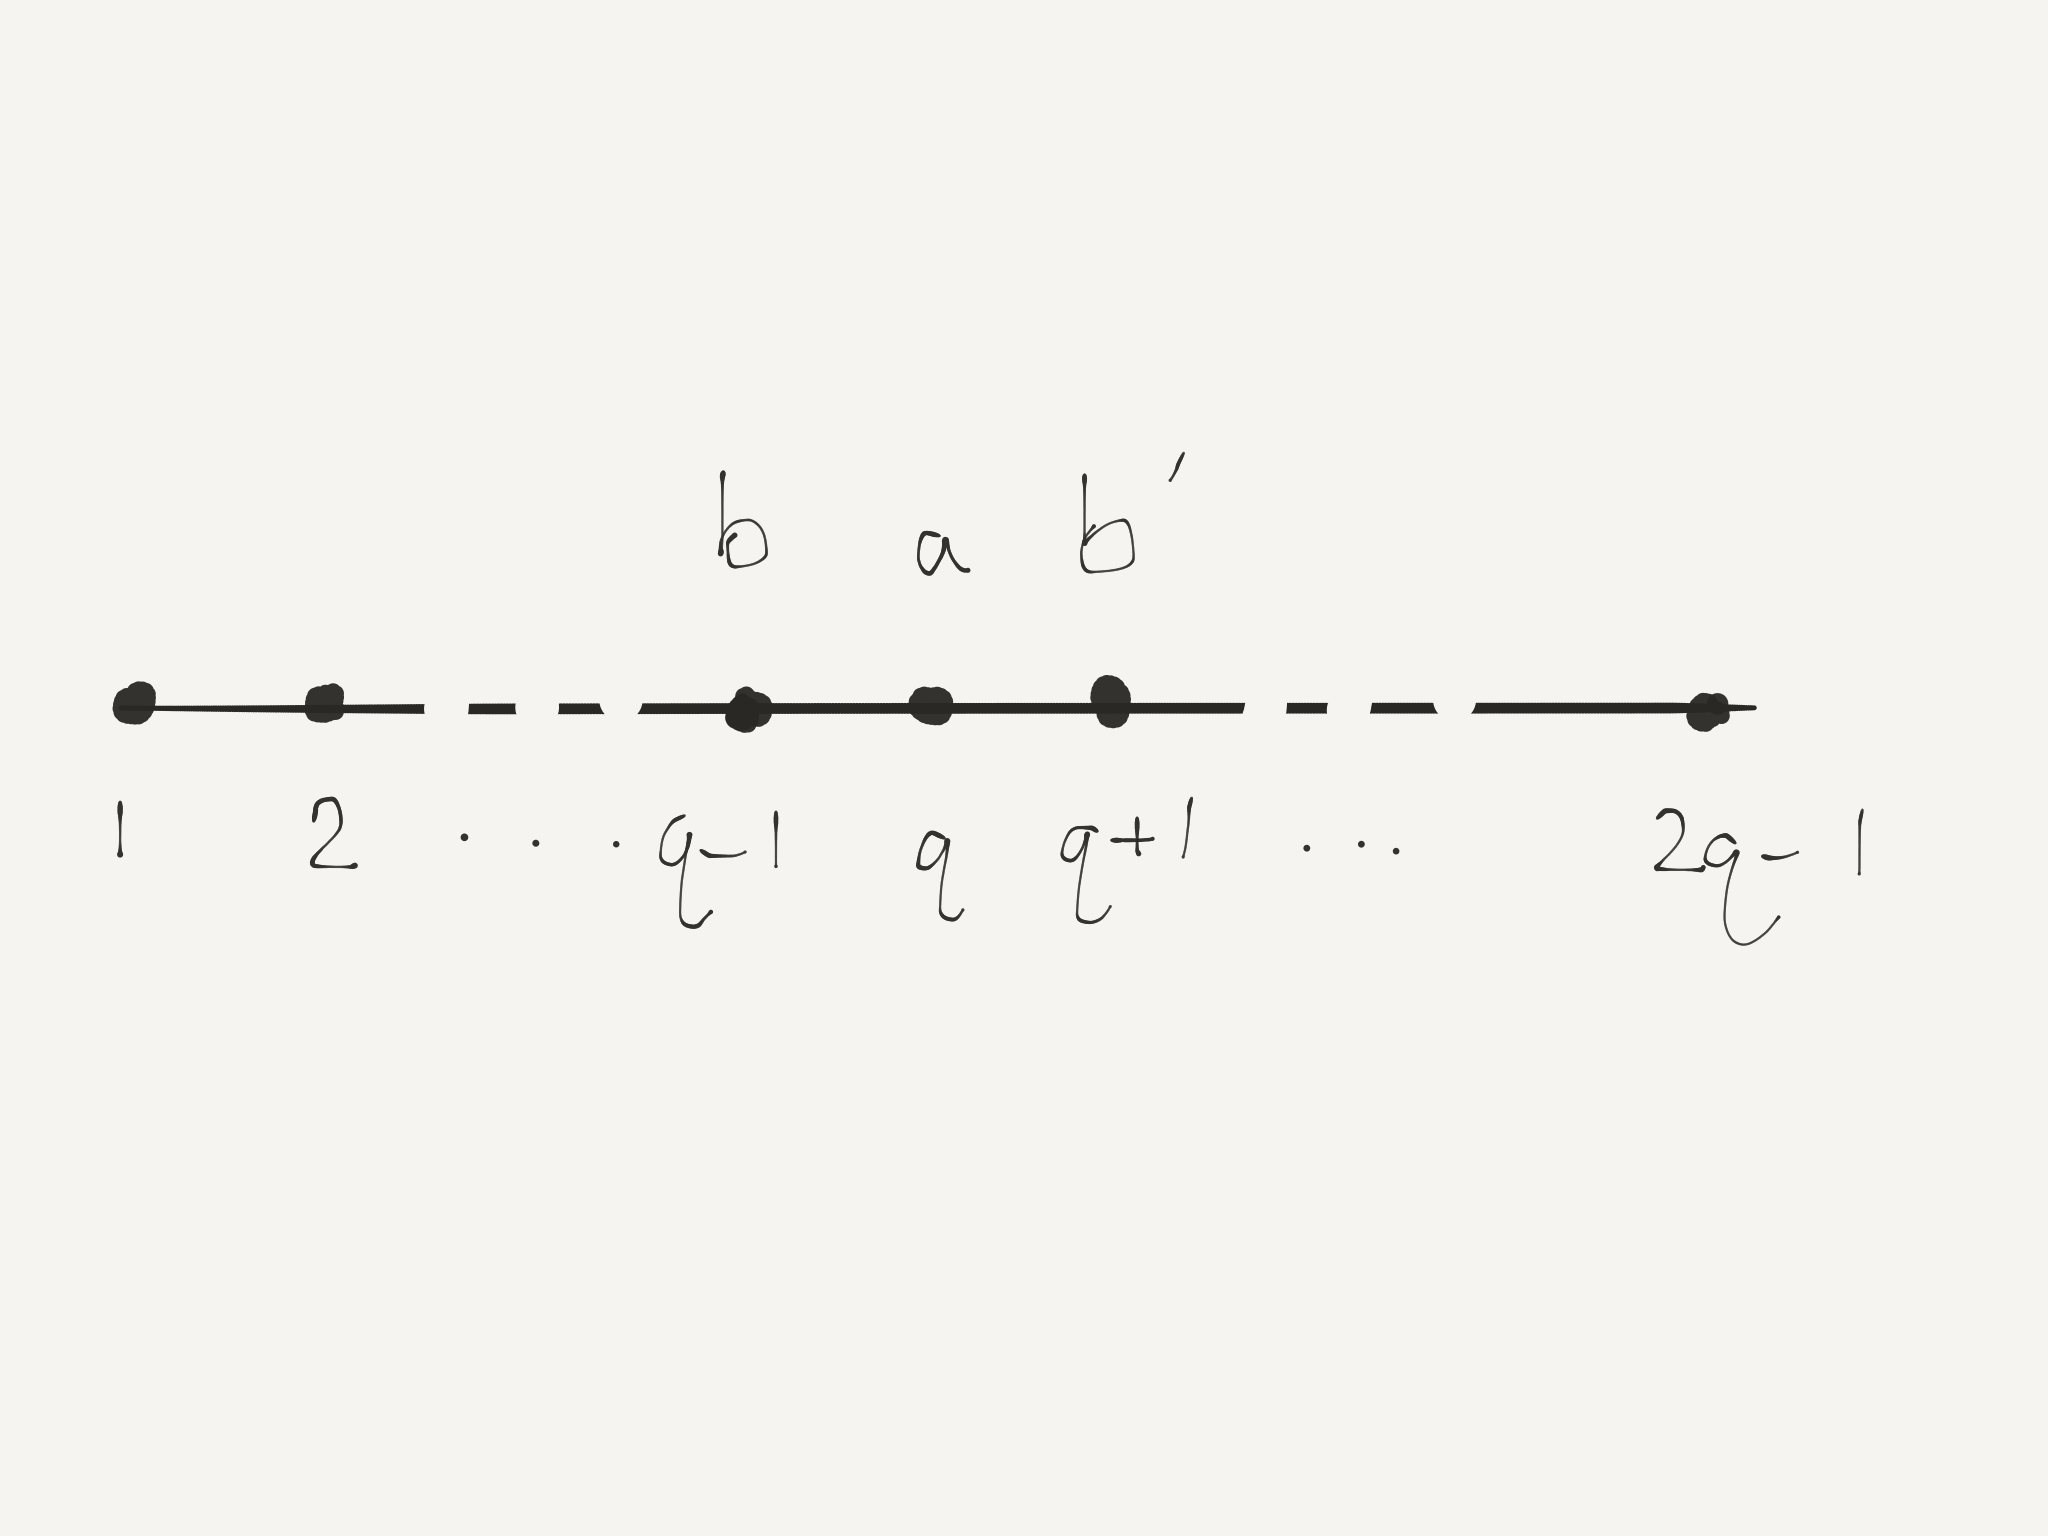
\includegraphics[scale=.2]{249-24.png}
\]
The $*$-action of $\Gamma$ goes through the quotient
$\Gal(k'/k)$ acting through flipping around the central 
vertex $a$, and the quotient $\Delta - \Delta_0 \twoheadrightarrow {}_k \Delta$
 modulo $\Gamma$ is depicted below. 
\[
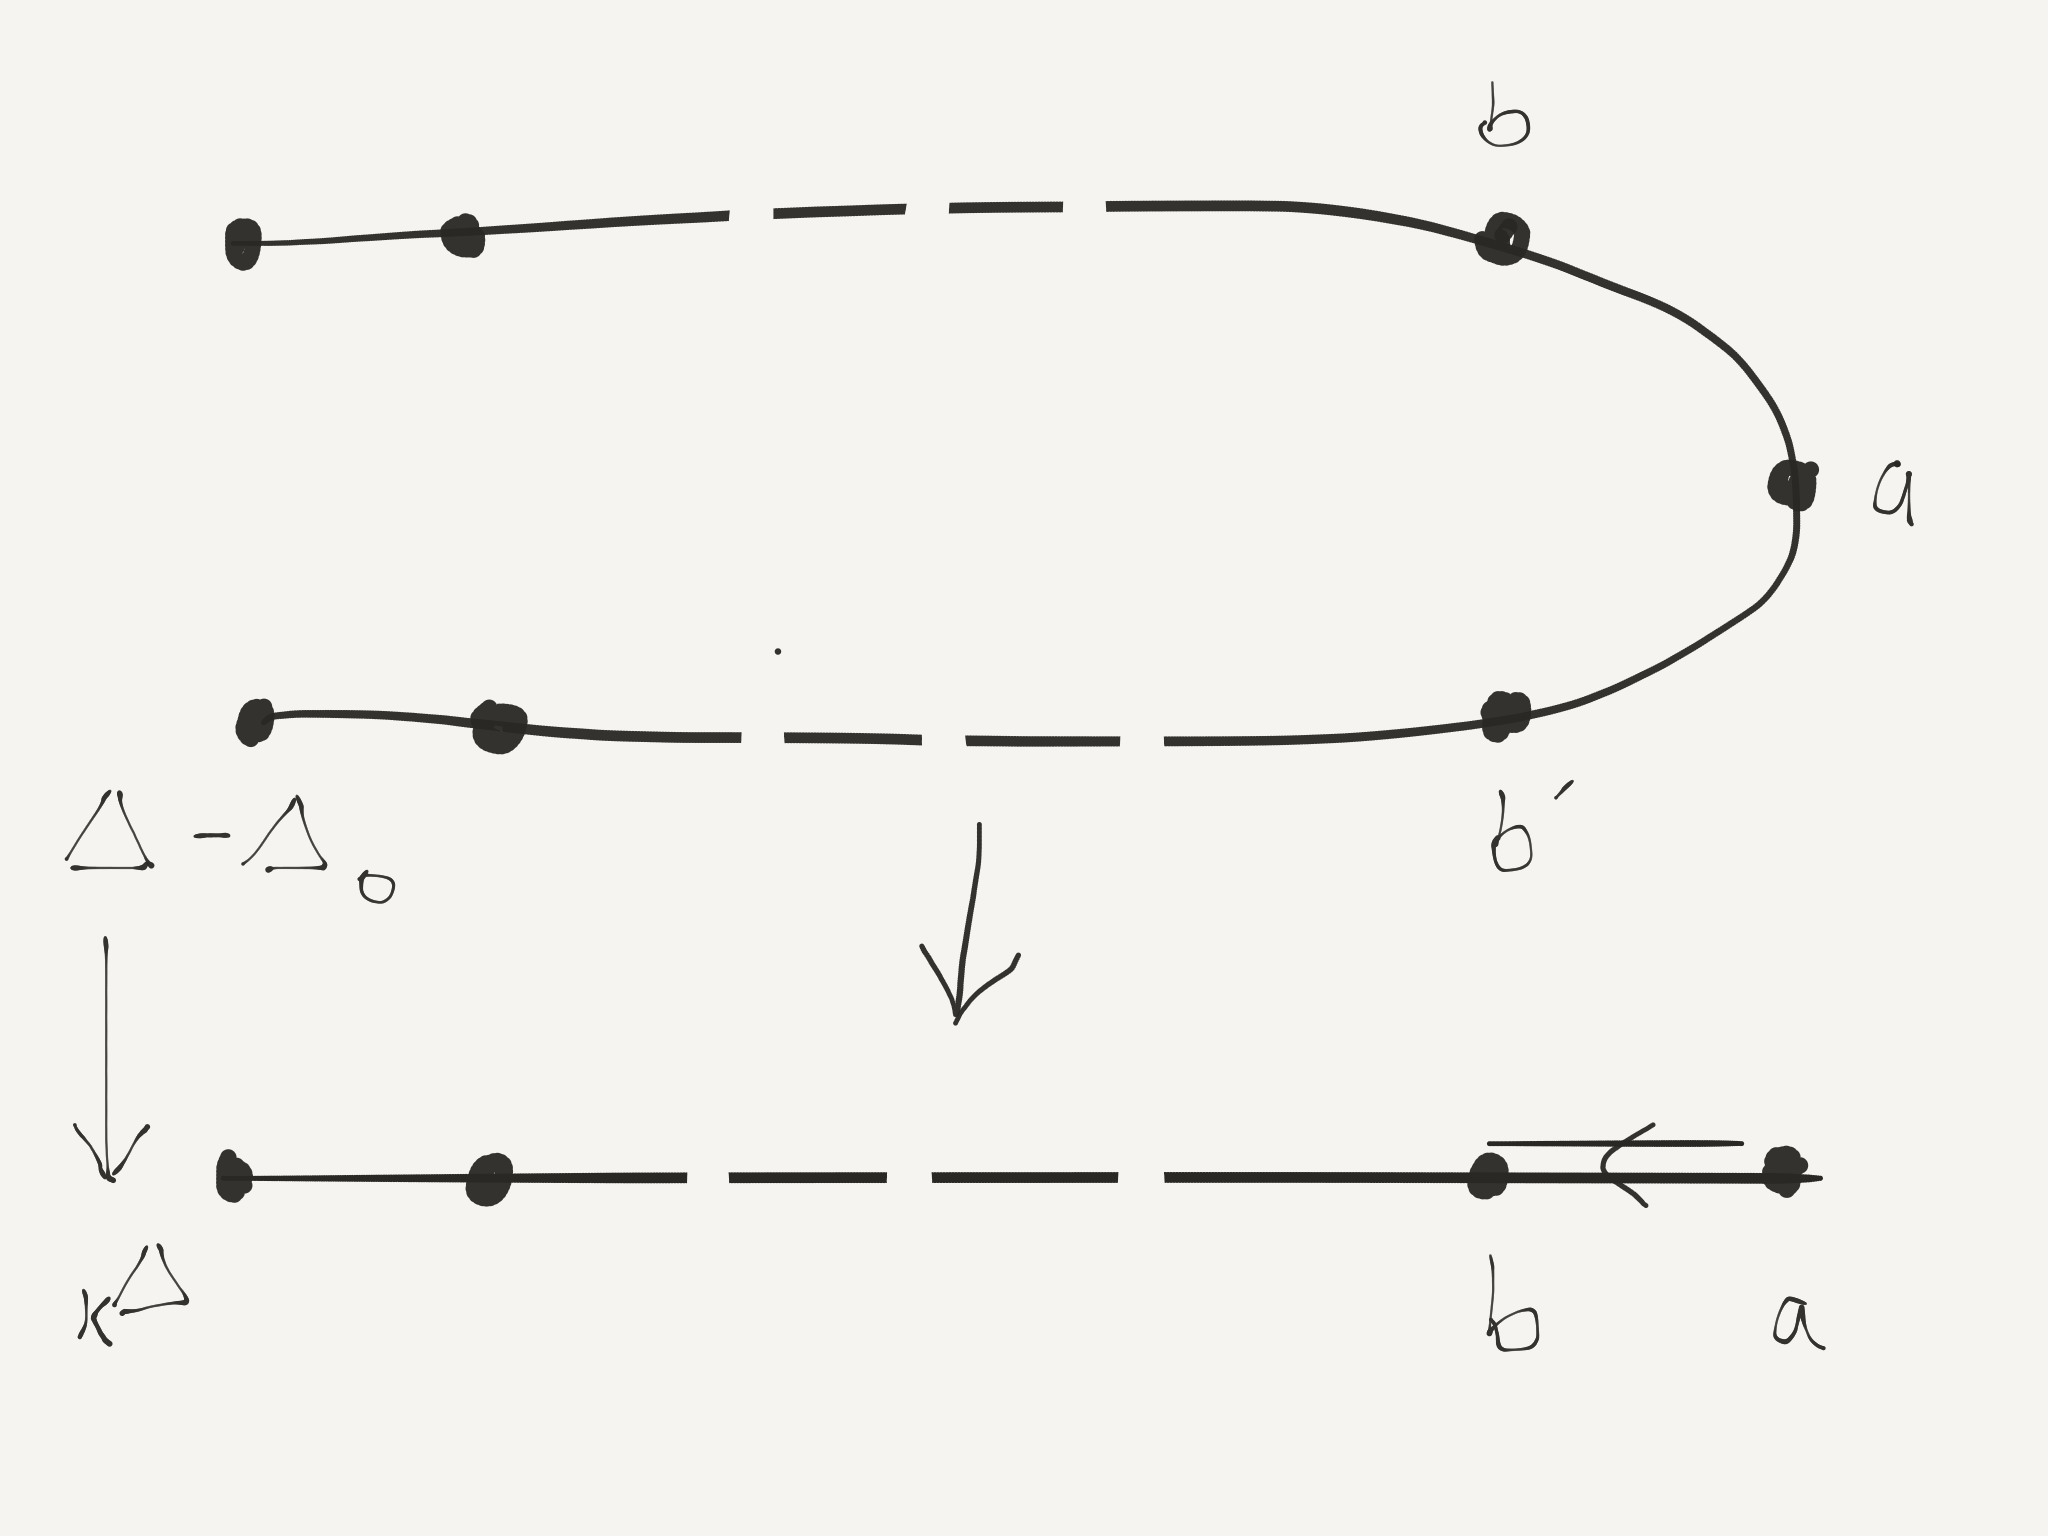
\includegraphics[scale=.2]{249-25.png}
\]
(The emptiness of $\Delta_0$ expresses that $G$ is quasi-split.)

How do we determine the edges (with multiplicity) in $_k \Delta$; e.g., that there is a double edge between the respective images $\overline{a}$ of $a$ and $\overline{b}$ of $b$ and $b'$, with $\overline{a}$
long and $\overline{b}$ short?   Rather than get involved with a general method, we explain
a hands-on argument in this case for analyzing the relationship between $\overline{a}$ and $\overline{b}$
(with the others easier to analyze by a similar method).
The quotient map $\Delta = \Delta - \Delta_0 \rightarrow {}_k\Delta$ corresponds to restriction of characters
along the inclusion $S_{k_s} \hookrightarrow T$, so 
$b$ and $b'$ restrict to a common character $\overline{b}$ distinct from the restriction
$\overline{a}$ of $a$, 
The subset $\{a,b,b'\}$ clearly spans an A$_3$ root system. 
The roots appearing are $a, b, b', a+b+b'$, as evidenced by the concrete model with $\SL_4$:
\[
\begin{pmatrix}
& b  &  a+b & a+b+b' \\ 
 & & a & a+b' \\
 & & & b' \\
 & & & &
\end{pmatrix}
\]
The images in $_k\Phi$ of the roots shown in the above $\SL_4$ picture
are $\ol{a}, \ol{b}, \ol{a}+\ol{b}, \ol{a}+2\ol{b}$. 

Recall that in any irreducible (possibly non-reduced) root system, for
any two roots $c$ and $c'$ the pairing $\langle c, {c'}^{\vee} \rangle$ 
is negative to the largest integer $j \ge 0$ such that $c + jc'$ is a root.  (This
was noted long ago, as an immediate consequence of inspection of the 
rank-2 root systems ${\rm{A}}_1 \times {\rm{A}}_1$, ${\rm{A}}_2$, ${\rm{B}}_2$, and ${\rm{G}}_2$.) 
Hence, $\langle \ol{a}, \ol{b}^{\vee} \rangle = -2$. 
Analyzing the other edges similarly, we obtain that $_k\Phi$ is of type C$_q$ (seen in a more explicit manner 
by arguments with big matrices in Appendix \ref{relroots}), 
for which the Dynkin diagram is as shown above with the vertex set ${}_k\Delta$. 
\end{example}

\begin{remark}
Any finite set with a continuous action of $\Gamma$ corresponds
canonically to a finite \'etale $k$-scheme.  The finite set $\Delta$ equipped with 
the $*$-action has associated finite \'etale $k$-scheme with an intrinsic meaning
in terms of $G$ without reference to a preferred choice of tori or Borel $k_s$-subgroup or minimal parabolic
$k$-subgroup:  it is the ``scheme of Dynkin diagrams'' 
in the sense of \cite{SGA3} (see the end of Appendix \ref{*-action} for a reference).  This is a fancy
way of expressing an alternative and more widely-known Kottwitz method (described near
the start of \S\ref{tsclass}) for removing 
the apparent dependence on auxiliary choices.
\end{remark}

The group $\Gamma$ 
acts on ${\rm{X}}(T_{k_s})$ via scalar 
extension along $k$-automorphisms of $k_s$, and using inversion on $\Gamma$
we likewise get an action (on the left!) on ${\rm{X}}_{\ast}(T_{k_s})$ 
that makes the pairing of characters and cocharacters $\Gamma$-invariant.
For $T' = T \cap \mathscr{D}(G)$ and the maximal central $k$-torus $Z$, 
these actions preserve the decompositions ${\rm{X}}(T_{k_s})_{\Q} = 
{\rm{X}}(T'_{k_s})_{\Q} \oplus {\rm{X}}(Z_{k_s})_{\Q}$ and the analogue for cocharacters.
Moreover, these actions factor through ${\rm{Gal}}(K/k)$ for any finite
Galois extension $K/k$ splitting $T$, so they are continuous.  

Note that $\Gamma$
preserves the finite subset $\Phi$ and is compatible with the natural action on $W(\Phi) =
N_G(T)(k_s)/T(k_s) = N_{\mathscr{D}(G)}(T')(k_s)/T'(k_s)$ 
and the $W(\Phi)$-action on ${\rm{X}}(T_{k_s})_{\Q}$, 
so by consideration of reflections in ${\rm{X}}(T'_{k_s}) = \Q \cdot \Phi$ the action 
on ${\rm{X}}_{\ast}(T'_{k_s})$ preserves $\Phi^{\vee}$ via the relation
$(\gamma.a)^{\vee} = \gamma.a^{\vee}$ for any $a \in \Phi$. 

\medskip

\noindent \textbf{Easy case of $*$-action.} Suppose $G$ is quasi-split, so $P$ is a Borel
$k$-subgroup (and $B = P_{k_s}$). The action on $\Phi$
certainly preserves $\Phi^+ = \Phi(B=P_{k_s}, T_{k_s})$, and so 
must preserve its basis $\Delta$. That resulting action of $\Gamma$ on $\Delta$ is easily checked
to be through diagram automorphisms (since it respects
pairings of roots and coroots), and to satisfy the desired properties.\\

In general, for $\gamma \in \Gamma$ clearly $\gamma(\Phi^+) \subset \Phi$ is a positive system of roots, so there exists a unique $w_{\gamma} \in W(\Phi) = N_G(T)(k_s)/T(k_s)$ 
such that $w_{\gamma}(\gamma(\Phi^+)) =  \Phi^+$, and so 
\[
w_{\gamma}(\gamma(\Delta)) = \Delta.
\]

Beware that generally $w_{\gamma}$ does not arise from $N_G(T)(k)$.   Note also that
away from the quasi-split case some $w_{\gamma}$ must be non-trivial.  Indeed,
$w_{\gamma} =1$ for all $\gamma$ if and only if $\Delta$ is $\Gamma$-stable, 
or equivalently $\Phi^+$ is $\Gamma$-stable, yet
$\gamma(\Phi^+) = \Phi(\gamma^{\ast}(B), T_{k_s})$ for any $\gamma \in \Gamma$, so
$w_{\gamma} = 1$ precisely when $\gamma^{\ast}(B) = B$ inside $G_{k_s}$.
Hence, that holds for all $\gamma$ precisely when $B$ is defined over $k$,
which is just another way to say that $G$ is quasi-split.

\begin{lemma}\label{wtrans}
The map 
\[
\Gamma \times {\rm{X}}(T_{k_s}) \rightarrow {\rm{X}}(T_{k_s})
\]
defined by $\gamma \ast a = w_{\gamma}(\gamma(a))$ preserving $\Delta$ 
  is a left action.
 The induced left action $($via the dual representation$)$ on ${\rm{X}}_*(T_{k_s})$ 
 preserves $\Delta^{\vee}$ via the relation $(\gamma \ast a)^{\vee} = \gamma \ast a^{\vee}$.
 
 By compatibility with the pairings of characters
 and cocharacters, this gives a left $\Gamma$-action on the Dynkin diagram. 
\end{lemma}

\begin{proof}
By definition-chasing, this comes down to establishing the equality 
\[
w_{\gamma' \gamma} = w_{\gamma'} \cdot \gamma'(w_{\gamma})
\]
in $W(G, T) = W(\Phi)$. That in turn can be verified by applying both sides to 
the positive system of roots $\gamma' \gamma (\Phi^+)$. 
\end{proof}

The quotient map ${\rm{X}}(T_{k_s}) \twoheadrightarrow {\rm{X}}(S_{k_s}) = {\rm{X}}(S)$
is certainly invariant for the natural $\Gamma$-action on the source (why?), and
it is also visibly invariant by the induced action of $N_{Z_G(S)}(T)(k_s)$ on the source (why?), so
to prove invariance of the restriction map $\Delta \rightarrow {}_k\Delta \cup \{0\}$ with respect to
the $\ast$-action on the source it suffices to prove:

\begin{proposition}\label{weyl_galois_compat}
Each $w_{\gamma}$ can be chosen to arise from $N_{Z_G(S)}(T)(k_s)$.
\end{proposition}

\begin{proof}
The point is that $\gamma(\Phi^+) $ is not an arbitrary positive system of roots inside $\Phi$: it satisfies
\[
\gamma(\Phi^+) \subset \gamma(\Phi(P_{k_s}, T_{k_s})) = \Phi(P_{k_s}, T_{k_s}).
\]
Thus, $\gamma(\Phi^+)$ corresponds to a Borel $k_s$-subgroup of $G_{k_s}$
contained in $P_{k_s}$ and containing $T_{k_s}$. Since
 $P = Z_G(S) \ltimes U$,  $N_{Z_G(S)}(T)(k_s)$ acts transitively on the set of Borels of $P_{k_s}$ containing $T_{k_s}$ because this can be checked modulo $U_{k_s}$ (as $U_{k_s}$ is contained in every Borel 
 $k_s$-subgroup of $P_{k_s}$, and $P_{k_s}/U_{k_s} = Z_G(S)_{k_s}$ is reductive). 
\end{proof}

\begin{lemma}\label{wgr}
Such $w_{\gamma}$ are generated by reflections in $\Delta_0$.
\end{lemma}

\begin{proof}
The root system $\Phi(Z_G(S)_{k_s}, T_{k_s})$ has $\Delta_0$ as a basis by Remark \ref{d0basis}.
\end{proof}

This establishes property (*1) formulated near the start of 
\S\ref{saction}. What about property (*2)? Consider $Q \leftrightarrow \Delta_0 \sqcup \Delta'$. What subset of $\Delta$ corresponds to $\gamma^*(Q) \supset \gamma^* (P_{k_s}) = P_{k_s}$? 

\begin{proposition}
We have $\gamma^*(Q) \leftrightarrow \Delta_0 \sqcup (\gamma * \Delta') = \gamma * (\Delta_0 \sqcup \Delta'))$. 
In particular, $\gamma^{\ast}(Q) = Q$ if and only if $\gamma \ast \Delta' = \Delta'$,
so $Q$ is defined over $k$ if and only if $\Delta'$ is $\Gamma$-stable under the $\ast$-action. 
\end{proposition}

\begin{proof}
For the full proof see \S2 of Appendix \ref{*-action}. The key is to show that $\gamma*(\Delta') \subset \gamma(\Delta') + \Z \Delta_0$, which ultimately follows from Corollary \ref{wgr} due to 
the general reflection formula $r_a(b) = b - \langle b, a^{\vee} \rangle a \in b + \Z a$
for $a, b \in \Phi$.
\end{proof}

We end our initial discussion of the $\ast$-action with an overview of its
role in the definition of the Langlands dual group.
Let $R = ({\rm{X}}(T_{k_s}), \Phi, {\rm{X}}_{\ast}(T_{k_s}), \Phi^{\vee})$ 
be the associated root datum over $k_s$.  
In the quasi-split case, we have seen that 
the $\ast$-action of $\Gamma$ on the based root datum $(R, \Delta)$
is induced by the natural $\Gamma$-action on ${\rm{X}}(T_{k_s})$.  In general, this action 
has significance going beyond its role in the Tits--Selbach classification: it also underlies
the definition of the {\em Langlands dual group}, as we now sketch.

Let $B \subset G_{k_s}$ be the unique Borel $k_s$-subgroup
containing $T_{k_s}$ such that $\Phi(B, T_{k_s})$ is the positive system of roots with basis $\Delta$, and let
$\{X_a\}_{a \in \Delta}$ be a pinning
(i.e., choice of basis of $\mathfrak{g}_a$ for each $a \in \Delta$).
The Isomorphism Theorem gives that the natural map
$${\rm{Aut}}_{k_s}(G_{k_s}, T_{k_s}, \{X_a\}_{a \in \Delta}) \rightarrow {\rm{Aut}}(R, \Delta)$$
is bijective.  That is, every automorphism of the based root datum uniquely lifts
to a $k_s$-automorphism of the ``pinned'' split reductive pair.

Since $\Delta$ is a basis of ${\rm{X}}((T/Z_G)_{k_s})$,
any change in $(T, \Delta)$ is attained by composing with the effect of an element of 
$(G/Z_G)(k_s)$ unique modulo $(T/Z_G)(k_s)$ (exercise!).  Thus, the lifting of ${\rm{Aut}}(R, \Delta)$ into
${\rm{Aut}}(G_{k_s})$ via a pinning is well-defined up to the effect of
$(G/Z_G)(k_s)$.  (This is the main content of the fact that the automorphism scheme 
${\rm{Aut}}_{G/k}$ has identity component $G/Z_G$ and component group that is
a $k_s/k$-form of ${\rm{Aut}}(R, \Delta)$.)

Now suppose $k$ is a local or global field, and let $W_k$ be the Weil group of $k$.
Let ${}^LG^0$ be the unique pinned connected reductive $\CC$-group whose root datum is
equipped with an identification with the dual root datum $R^{\vee} = ({\rm{X}}_{\ast}(T_{k_s}), \Phi^{\vee}, {\rm{X}}(T_{k_s}), \Phi)$.  
The $\ast$-action defines a composite homomorphism
$$\rho:\Gamma \rightarrow {\rm{Aut}}(R^{\vee}, \Delta^{\vee}) \hookrightarrow
{\rm{Aut}}({}^LG^0)$$
whose second step rests on the choice of pinning of ${}^LG^0$ (applying the preceding discussion with $k = \CC$), 
so the {\em ${}^LG^0(\CC)$-conjugacy class} of this
homomorphism is independent of all choices.  If $k'/k$ is a finite Galois subextension of
$k_s$ such that $G_{k'}$ is split then ${\rm{Gal}}(k_s/k')$ acts trivially on $\Delta$ under
the $\ast$-action as defined above, so $\rho$ factors through ${\rm{Gal}}(k'/k)$.  The {\em Langlands dual}
is the disconnected locally algebraic group
$${}^LG := \Gamma \ltimes {}^LG^0;$$
this group is only well-defined up to ${}^LG^0(\CC)$-conjugation.
(The main content occurs ``at finite level'', using the typically disconnected linear algebraic $\CC$-group
${\rm{Gal}}(k'/k) \ltimes {}^LG^0$.) 
Hence, the notion of {\em ${}^LG^0(\CC)$-conjugacy class} of  continuous homomorphism
$$\phi:W_k \rightarrow {}^LG(\CC)$$
over the natural map $W_k \rightarrow \Gamma$
is intrinsic to the $k$-group $G$.  Such conjugacy classes, or variants  with $W_k$ replaced by
the Weil--Deligne group, are of central importance in the Langlands Program.
(If $G$ is a split group then ${}^LG = \Gamma \times {}^LG^0$ and such $\phi$
are exactly conjugacy classes of continuous homomorphisms $W_k \rightarrow {}^LG^0(\CC)$.)

\begin{example}
In the special case that $G$ is a $k$-torus $T$, so there are no absolute roots
and the $\ast$-action is just the natural $\Gamma$-action on ${\rm{X}}(T_{k_s})$, 
we have ${}^LT = \Gamma \ltimes \widehat{T}$
where the {\em dual torus} $\widehat{T}$ is $\underline{{\rm{Hom}}}({\rm{X}}(T_{k_s}), \G_m)$
on which $\Gamma$ acts via the natural action on the geometric character lattice.
The homomorphisms $\phi: W_k \rightarrow {}^LT(\CC) = \Gamma \ltimes \widehat{T}(\CC)$
have second component that is exactly a continuous 1-cocycle $f:W_k \rightarrow \widehat{T}(\CC)$,
and the effect of composing $\phi$ with a $\widehat{T}(\CC)$-conjugation is exactly to change
$f$ by a 1-coboundary.  

Note that if $T$ splits over a finite Galois extension
$k'/k$ inside $k_s/k$ then the $\ast$-action on ${\rm{Gal}}(k_s/k')$ is trivial, so $f|_{W_{k'}}$ is just
a continuous homomorphism by another name. But  the target of $f$ is commutative, so $f$
must kill the commutator subgroup of $W_{k'}$.
By the construction of $W_k$ using class formations in \cite[Ch.\,XV]{at} (the only unified approach
that treats all local and global fields on an equal footing and provides the only known definition
for $W_k$ when $k$ is a number field), the quotient of $W_k$ modulo the commutator subgroup of $W_{k'}$
is the group $W_{k'/k}$ that is naturally a topological extension of ${\rm{Gal}}(k'/k)$ by
$A(k)$, where $A(k) = 
\mathbf{A}_k^{\times}/k^{\times}$ in the global case and  $A(k) = k^{\times}$ in the local case
(this extension representing the fundamental class associated to $k'/k$).  That is,
such 1-cocycles $f$ arise from 1-cocycles $W_{k'/k} \rightarrow \widehat{T}(\CC)$. 

An early verification of Langlands \cite[Thm.\,2]{tori} was that for any local field $k$ there is a ``natural''
isomorphism from ${\rm{H}}^1_{\rm{cont}}(W_k, \widehat{T}(\CC))$ onto the group 
continuous homomorphisms $T(k) \rightarrow \CC^{\times}$, and that for any global field $k$
there is a ``natural'' surjection with finite (explicitly
described) kernel from ${\rm{H}}^1_{\rm{cont}}(W_k, \widehat{T}(\CC))$
onto the group of continuous homomorphisms
$T(\mathbf{A}_k)/T(k) \rightarrow \CC^{\times}$. 
These ``natural'' maps are specific
constructions (satisfying good properties), 
called {\em Langlands duality for tori}, and for $T = \G_m$ by design this recovers
the construction made via Artin reciprocity maps in class field theory. 
\end{example}

\subsection{Relative root groups}

As a companion to the use of the relative root system to keep track of parabolic $k$-subgroups,
there is a theory of (high-dimensional, and possibly non-commutative) relative root
groups.  These satisfy many of the familiar properties of root groups in the split
case, including to give a concrete description of Levi factors and unipotent radicals
of parabolic $k$-subgroups.  We will record the main results (which are unsurprising once
the definitions are given) and {\em refer to Appendix {\rm{\ref{roottits}}}
for the proofs}. 

But first we address a loose end from our earlier discussion of Levi factors of parabolic subgroups:
we know that if $P$ is a parabolic $k$-subgroup of a connected reductive $k$-group $G$
and $U := \mathscr{R}_{u,k}(P)$ is the split $k$-descent of its geometric
unipotent radical (by writing $P = P_G(\lambda)$ for
a $k$-homomorphism $\lambda: \G_m \rightarrow G$ we have $U = U_G(\lambda)$),
there exists a $k$-subgroup $L$ such that $L \rightarrow P/U$ is an isomorphism,
or equivalently $L \ltimes U = P$; e.g., for a dynamic description $P_G(\lambda)$ of $P$
we can take $L$ to be $Z_G(\lambda)$.  The $k$-isomorphism class of $L$
is obviously intrinsic (after all, $L \rightarrow P/U$ is an isomorphism!), but
as a $k$-subgroup of $P$ how are the different choices related to each other?

In view of the use of Levi factors for calculations in representation theory, 
it would be best if all such $L$ are related through $P(k)$-conjugacy, or
equivalently (!) through $U(k)$-conjugacy.   Fortunately, this is true in the following more precise form:

\begin{proposition}\label{Lunique} The action of $U(k)$ on the set of Levi factors of $P$ is simply transitive.
Moreover, every maximal $k$-torus $T$ of $P$ is contained in a unique Levi factor of $P$.
\end{proposition}

Some Levi $k$-subgroups arise by the dynamic method, so the $U(k)$-conjugacy implies
that {\em all} Levi $k$-subgroups arise by the dynamic process!

\begin{proof} In view of the uniqueness assertion, by Galois descent it suffices
to treat the situation over $k_s$; i.e., we now may and do assume $k = k_s$, so all
$k$-tori are split.   We shall first prove that any maximal $k$-torus $T \subset P$
lies in a unique Levi factor $L$.  Since $T$ is maximal in $P$, we can write $P = P_G(\lambda)$ for some
$\lambda \in {\rm{X}}_{\ast}(T)$.  Hence, $Z_G(\lambda)$ is a Levi factor
of $P$ containing $T$.  To prove that there is at most one $L$ containing $T$,
we shall describe any such $L$ directly in terms of $T$ and $P$.

Consider the set $\Phi(L, T)$ of nontrivial $T$-weights that occur on ${\rm{Lie}}(L)$.
We have $L \simeq P/U$, so $\Phi(L, T) = \Phi(P/U, T)$
is independent of $L$ inside ${\rm{X}}(T)$.  Let $\Psi$ denote this subset of $\Phi = \Phi(G, T)$.
For each $a \in \Psi$, the $a$-root group for 
the connected reductive $L$  with respect to $T$
is {\em the same} as for $G$ by uniqueness of root groups
(as $T$-stable smooth connected unipotent $k$-subgroups
exhibiting a specific root line as their Lie algebra).
But $L$ is is generated by $T$ and the root groups $U_a$ for $a \in \Psi = \Phi(P/U, T)$.
The latter is a description of $L$ in terms of just $P$ and $T$, establishing
the uniqueness of $L$.

Since all maximal (split) $k$-tori of $P$ are $P(k)$-conjugate, the preceding
uniqueness result implies that all Levi factors of $P$ are $P(k)$-conjugate to each other,
and so are $U(k)$-conjugate to each other.
It remains to show that if $u \in U(k)$ normalizes a Levi factor $L$ then $u=1$.
For any $x \in L(k)$ we have $uxu^{-1} \in L(k)$, so $u(xu^{-1}x^{-1}) \in L(k)$.
But $U$ is normal in $P$, so $u(xu^{-1}x^{-1}) \in U(k)$.  Since
$L \cap U = 1$ it follows that $uxu^{-1}x^{-1} = 1$, which is to say that 
$u$ centralizes $L(k)$. Since $L(k)$ is Zariski-dense in $L$ (as $k=k_s$),
we have $u \in Z_G(L)(k) \subset Z_G(T)(k)$ for a maximal $k$-torus $T \subset G$.
But $Z_G(T)=T$, so $u \in T \cap U = 1$.
\end{proof}

\begin{example}\label{plu}
Consider $G$ containing a split maximal $k$-torus $T$, and let $I$ be a subset of a basis $\Delta$
of a positive system of roots $\Phi^+$ for $\Phi := \Phi(G, T)$.  Let $B$ be the Borel $k$-subgroup containing $T$
for which $\Phi^+ := \Phi(B, T)$.  For the parabolic $k$-subgroup ${}_kP_I$ containing $B$
we have $\Phi({}_k P_I, T) = \Phi^+ \cup [I]$, so 
the unique Levi $k$-subgroup $L_I$ containing $T$ satisfies
$\Phi(L_I, T) = [I]$ (argue exactly as in Remark \ref{d0basis}).  

We can describe $L_I$ explicitly as follows.  Consider
the subtorus $T_I = (\cap_{a \in I} \ker a)^0_{\rm{red}} \subset T$.
The connected
reductive $k$-group $Z_G(T_I)$ containing $T$ is generated by $T$
and the root groups $U_a$ for roots $a$ trivial on $T_I$, which is to say 
$a \in [I]$ (as $I$ is part of a basis $\Delta$ for $\Phi$).  But by the same reasoning
$L_I$ is generated by the same subgroups since $\Phi(L_I, T) = [I]$.
Hence, $L_I = Z_G(T_I)$.

Writing ${}_k P_I = P_G(\lambda)$ for some $\lambda \in {\rm{X}}_{\ast}(T)$,
so $U_I := \mathscr{R}{u,k}({}_kP_I) = U_G(\lambda)$,
we have $U_I = \prod_{a \in \Phi(U_I, T)} U_a$
(with multiplication in any order) by 
Theorem \ref{3311} applied to $A = \Phi_{\lambda > 0}$ with $A_j$ its singleton subsets
($\Phi$ is reduced!), and the collection of roots $\Phi(U_I, T)$ is exactly $\Phi^+ - [I]$ because 
${}_k P_I = \Phi^+ \cup [I]$ and $\Phi(L_I, T) = [I]$.
\end{example}

We would like to push Example \ref{plu} beyond the split setting, to describe
${}_kP_I$ in terms of specific root groups $U_a$ attached to relative roots $a \in {}_k\Phi$
and the centralizer of a specific subtorus $S_I \subset S$.  But to do
this we first need to {\em define} what $U_a$ means beyond the split case!
Recall that in the split case we use a dynamical construction,
namely $U_{\langle a \rangle}(G)$ to define $U_a$, and then
used $\SL_2$-calculations to deduce that $U_a$ is a 1-dimensional vector group.
Moreover, dynamical principles (and {\em not} $\SL_2$-calculations as in standard
textbooks) were used to deduce directly spanning results and commutation relations among root
groups, sometimes relying on reducedness of $\Phi$ to ensure
any two distinct roots inside a positive system of roots are linearly independent.

Provided that we are attentive to whether roots are divisible or multipliable (or neither),
much of the previous work carries over {\em unchanged} to the general case,
including the definition of $U_a$: define it to be $U_{\langle a\rangle}(G)$.  There are some new features:
\begin{itemize}
\item[(i)] without the $\SL_2$-crutch, we don't immediately see whether or not $U_a$ is a vector group
(is it even commutative?), nor if so whether it has a preferred linear structure (a genuine issue in higher dimensions
since in characteristic $p > 0$ the $k$-group $\mathbf{G}_{\rm{a}}^2$ has non-linear automorphisms
such as $(x, y) \mapsto (x + y^p, y)$),
\item[(ii)] The set of $S$-weights on ${\rm{Lie}}(U_a)$ is ${}_k\Phi \cap \Z_{\ge 0} a$ by design,
and this is $\{a, 2a\}$ when $a$ is multipliable, so this Lie algebra can be larger than a single weight space.
\end{itemize}
The groups ${\rm{SU}}(h)$ exhibit all of these issues (including that $U_a$ can be non-commutative
for multipliable $a$).

Fortunately, {\em dynamical methods} (having nothing to do with reductive groups) in
\cite[\S3.3]{pred} dispose of all of these
problems:  $U_a$ is always a vector group when $2a \not\in {}_k \Phi$,
and in the multipliable case (so $U_{2a}$ is a vector group, as $4a \not\in {}_k\Phi$!)
the vector group $U_{2a}$ is a {\em central} $k$-subgroup of $U_a$ with $U_a/U_{2a}$
also a vector group, and moreover that all of these vector groups
admit a unique $S$-equivariant linear structure.   These matters
are discussed at length in Appendix \ref{roottits}, 
the upshot of which is that (with a bit more work required in a few places) one has reasonable analogues
of all of the familiar features of root groups from the split case, so here we just wish to  highlight
two aspects:
\begin{itemize}
\item[(1)] For $I \subset {}_k\Delta$, the parabolic $k$-subgroup 
${}_kP_I$ has a unique Levi $k$-subgroup $L_I \supset S$ (improving on Proposition \ref{Lunique}!)
and both $L_I$ and $U_I$ are described by the analogue of Example \ref{plu}
using $S$ and ${}_k\Delta$ and the set of non-divisible elements of ${}_k\Phi^+ - [I]$.
(This ``direct spanning'' description of $U_I$ is crucial for calculations in the foundations
of Bruhat--Tits theory.)
\item[(2)] If $G$ is semisimple, $k$-simple, and isotropic then ${}_k\Phi$ is {\em irreducible}
(often non-reduced!) and $G$ is generated by the relative root groups $U_a$ for $a \in {}_k\Phi$.
The proof of this result is {\em much harder} than its counterpart in the split case
(as the structure of $Z_G(S)$ a mystery,
and we cannot increase $k$ since that may change the relative root system and ruin the maximality of $S$).
\end{itemize}

For $k$-simple isotropic $G$, the simply connected central cover of $G$ is also
$k$-simple. Hence, by Corollary \ref{corres}, that cover has the form ${\rm{R}}_{k'/k}(G')$ 
for a canonically determined finite separable
extension $k'/k$ and connected semisimple $k'$-group $G'$
that is {\em absolutely simple} and simply connected.  

The relative root datum of ${\rm{R}}_{k'/k}(G')$ is identified with that of $G'$
(see \S2 of Appendix \ref{relroots}), so 
for the purpose of describing the possibilities for connected semisimple groups over a field
in terms of the relative root system and $\ast$-action on the absolute diagram (and perhaps further information), 
the essential case is that of absolutely simple groups
(which are moreover simply connected). 

\subsection{Tits-Selbach classification}\label{tsclass}
Let $G$ be a connected semisimple $k$-group, $S \subset G$ a maximal split $k$-torus. 

\begin{theorem} If $S$ is maximal $($as a $k$-torus$)$ 
in $G$ then the reduced root datum $R(G,S)$ is a complete isomorphism invariant. 
\end{theorem}

By ``complete invariant'' we mean that every reduced root datum actually arises from a split
reductive pair over $k$ (the Existence Theorem) and that two split connected reductive $k$-groups
are isomorphic if their root data are isomorphic (the Isomorphism Theorem).

In the general case, we get the following data from $G$:

\begin{enumerate} 
\item The Dynkin diagram $\Dyn(G)$ with $*$-action given by $\Gamma = \Gal(k_s/k)$. A priori this depends upon a choice of $S \subset T \subset P$ and $T_{k_s} \subset B \subset P_{k_s}$. However, we can suppress the auxiliary choices by using either of the following viewpoints:
\begin{itemize}
\item the finite \'{e}tale $k$-scheme of Dynkin diagrams, or 
\item the ``Kottwitz method'': if $T'$ and $T'_{k_s} \subset B' \subset P_{k_s}$ are another pair
for the same $S$ and $P$ then there exists $g \in G(k_s)$ such that $B' = gBg^{-1}$ and
$T'_{k_s} = gT_{k_s}g^{-1}$, with $g$ unique up to right multiplication against $B \cap N_G(T)_{k_s} = 
T_{k_s}$, so the isomorphism of diagrams $\Delta(B, T_{k_s}) \simeq \Delta(B', T'_{k_s})$
induced by $g$-conjugation is {\em independent} of the choice of $g$. This independence
ensures that it is compatible with the $\ast$-actions on both sides, and likewise if we
vary the initial pair $(S, P)$.  This canonically identifies all such diagrams
(i.e., we can declare ${\rm{Dyn}}(G)$ to be the inverse limit
of all diagrams $\Delta(B, T_{k_s})$ along these specified canonical $\Gamma$-compatible
diagram isomorphisms as we vary $(B, T)$ and then vary $(S, P)$). 
\end{itemize}
The significance of a viewpoint that avoids reliance on a specific choice of auxiliary
data is that it makes the $\ast$-action of $\Gamma$ on $\Dyn(G)$ 
functorial with respect to {\em any} $k$-isomorphism in $G$.  That is, if
$f:G' \simeq G$ is a $k$-isomorphism then we get a canonically associated
diagram isomorphism ${\rm{Dyn}}(f)$ that is compatible with $\ast$-actions on both sides.

\item $M = \Cal{D}(Z_G(S)/S)^{\ad}$ is $k$-anisotropic connected semisimple of adjoint type. 

\item There are canonical identifications 
\[
\xymatrix{
\Delta_0 := \{ a \in \Delta \mid a|_{S_{k_s}}=1\}   \ar@{=}[r]  \ar@{^{(}->}[d] & \Dyn(M)   \ar@{^{(}.>}[d] \\
\Delta \ar@{=}[r] & \Dyn (G)
}
\]
inducing a canonical inclusion $\Dyn(M) \hookrightarrow \Dyn(G)$ which is \emph{$\Gamma$-invariant}. This is not obvious because the $*$-action depends on the Weyl action, but follows from Proposition \ref{weyl_galois_compat}, which says that $w_{\gamma}$ in the definition of the $*$-action on $\Dyn(G)$ comes from $N_{Z_G(S)}(T)(k_s)$.
\end{enumerate}

\begin{example} Let $D$ be a central division algebra over $k$ of dimension $d^2$, and $G = \SL_m(D)$. Then $G$ is of type $A_{n-1}$ where $n=md$. The maximal split torus $S$ is of dimension $m$, consisting of the diagonal scalars in 
\[
S = \left\{\begin{pmatrix} {\rm{GL}}_1 \\ & {\rm{GL}}_1 \\
& & \ddots \\ 
& & & {\rm{GL}}_1 \end{pmatrix} \right\} \subset \left\{g \in \begin{pmatrix} \underline{D} & \underline{D} &  \ldots & \underline{D} \\
\underline{D} & \underline{D} & \ldots & \underline{D} \\
\vdots & \ddots & \ddots & \vdots \\
\underline{D} &\underline{D} &\underline{D}  & \underline{D} \end{pmatrix}\,\,|\,\, {\rm{Nrd}}(g)=1 \right\}
\]
where ${\rm{Nrd}}: {\rm{Mat}}_m(D) \rightarrow k$ is the reduced norm
and $\underline{D}$ is the affine ring scheme associated to $D$
(i.e., represents the functor on $k$-algebras given by
$A \rightsquigarrow A \otimes_k D$). 
The centralizer $Z_G(S)$ is then the diagonal matrices:
\[
Z_G(S) = \left\{\begin{pmatrix} \underline{D}^{\times} \\ & \underline{D}^{\times} \\
& & \ddots \\ 
& & & \underline{D}^{\times} \end{pmatrix} \right\} \subset \left\{ \begin{pmatrix} \underline{D} & \underline{D} &  \ldots & \underline{D} \\
\underline{D} & \underline{D} & \ldots & \underline{D} \\
\vdots & \ddots & \ddots & \vdots \\
\underline{D} &\underline{D} &\underline{D}  & \underline{D} \end{pmatrix} \right\}.
\]
Therefore $M = (\underline{D}^{\times}/\GL_1)^m$. 

The Dynkin diagram is depicted below, with roots in $\Delta_0$ circled
and the roots in $\Delta-\Delta_0$ marked with black dots:
\[
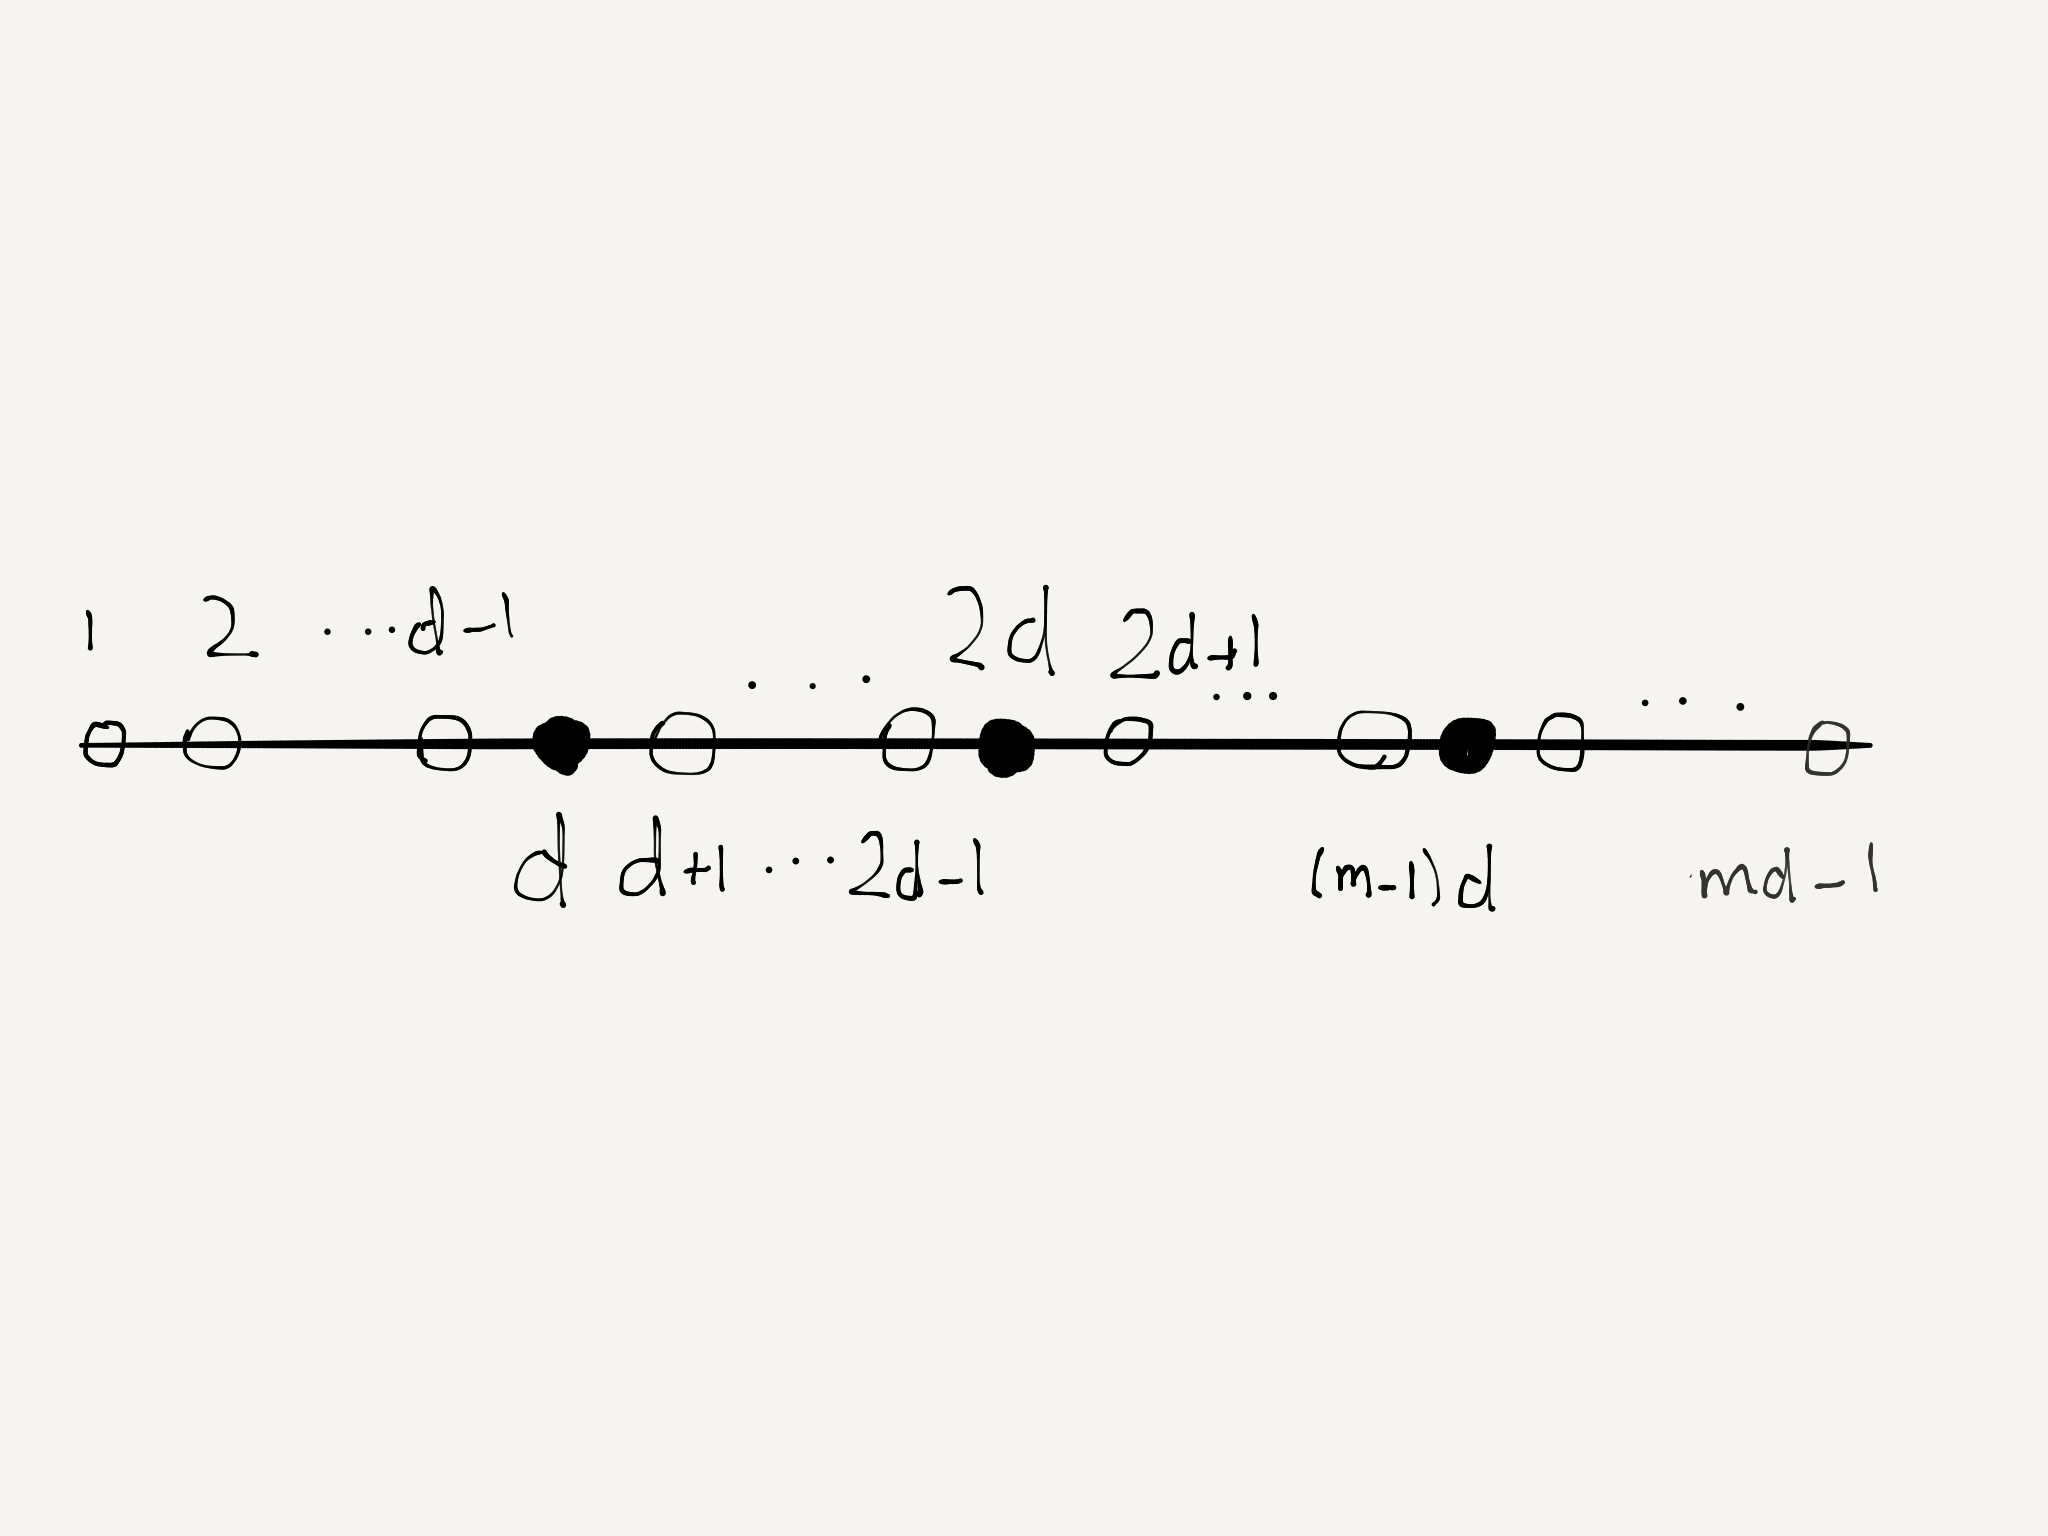
\includegraphics[scale=.25]{249-26.png}
\]
The $\Gamma$-action is trivial. We have $\Delta_0 = {\rm{A}}_{d-1}^m$ and $_k \Delta = {\rm{A}}_{m-1}$. 


\end{example}



From $G$ we get a 4-tuple $(R, \tau , M, j)$ where
\begin{itemize}
\item $R$ is a semisimple root datum, 
\item $\tau$ is a continuous action of $\Gamma$ on $\Dyn(R)$,
\item $M$ is a $k$-anisotropic group of adjoint type, 
\item $j \colon (\Dyn(M), *) \hookrightarrow (\Dyn(\Cal{R}), \tau)$ is a $\Gamma$-invariant inclusion. 
\end{itemize}
There is an evident notion of isomorphism among such 4-tuples, and 
the isomorphism class of the 4-tuple we obtain from $G$ is easily checked (do it!)
to be independent of all choices; i.e., it only depends on the isomorphism class of $G$. 

\begin{remark}
 The $k$-group $M$ is a mystery
 over general fields, usually entailing involvement of
 central division algebras, anisotropic quadratic or hermitian forms, and so on
 (e.g., for a general field $k$, ${\rm{Br}}(k)[2]$ may contain
 classes of central division algebras beyond dimension 4).  Over local and global
 fields this data is understood via class field theory.
 \end{remark}
 
 The main result announced by Tits \cite[2.7.1]{tits66} and completed by Selbach \cite{selbach} is:
 
\begin{theorem}[Relative Isomorphism Theorem] The association from $G$ to this 4-tuple is injective on isomorphism classes. 
\end{theorem}

On its own, the  statement of this theorem is not as useful as it may seem to be (in contrast with the split case),
since to actually determine which 4-tuples can arise
over a given $k$ generally entails a lot of effort specific
to a given root system. In practice, the importance of this theorem is two-fold:
\begin{itemize}
\item[(i)] it provides a useful framework to organize the information that arises in the analysis of possible $k$-groups
with a given absolute semisimple root datum,
\item[(ii)] knowledge of the \emph{proof} of the theorem (in the format we will describe it),
especially the idea of ``reduction of the structure group'', 
helps very much to systematically analyze what $G$ may occur.
\end{itemize}
I've not been able to understand Tits' original exposition of his proof, but I am certain that 
his cocycle manipulations should amount to an alternative formulation of what is done in the proof-sketch 
below. (A difference between Tits' approach and the one
sketched below is that Tits uses the idea of the automorphism variety of
a split group over $k$ whereas we will work throughout with the automorphism variety
of a given connected semisimple $k$-group $G$ that is typically not split.) 

\begin{proof}[Idea of proof] The slogan is ``reduction of the structure group''!
We will need to use degree-1 non-abelian Galois cohomology;
this is a systematic technique for working with torsors
under smooth affine groups over a field, and is set up in \cite[Ch.,I, \S5.1--\S5.5]{SerreGaloisCohomology}. 
We will explain the basic idea behind this formalism, and then indicate how it is used.

Suppose $G$ and $G'$ give isomorphic 4-tuples.  By the Isomorphism Theorem
over $k_s$, the identification of their absolute root data implies
that $G'_{k_s} \simeq G_{k_s}$. 
Thus, there is some finite Galois extension $K/k$ inside $k_s/k$ (such
as any that splits choices of maximal $k$-tori in  $G$ and $G'$)
such that $G'_K \simeq G_K$ as $K$-groups.  This says that $G'$
can be obtained from $G$ by modifying the Galois
descent datum 
$$\{\varphi_{\gamma}: \gamma^{\ast}(G_K) \simeq G_K\}_{\gamma \in {\rm{Gal}}(K/k)}$$
which reconstructs $G$ from $G_K$.  (Any $K/k$-descent datum
on an affine scheme is always effective, via Galois descent for the coordinate ring.)

Upon fixing a $K$-isomorphism $f: G'_K \simeq G_K$, 
a descent datum $\{\varphi'_{\gamma}\}$ encoding $G'$ as a $K/k$-form of $G$
is given by 
$$\varphi'_{\gamma}: \gamma^{\ast}(G_K) \simeq \gamma^{\ast}(G'_K) \simeq G'_K \simeq G_K$$
(using the $k$-descent $G'$ of $G'_K$ for the middle isomorphism).  We can write
$\varphi'_{\gamma} = c(\gamma)\varphi_{\gamma}$
for a unique $K$-automorphisms $c(\gamma): G_K \simeq G_K$,
and the condition that $\varphi'$ be a descent datum (given that $\varphi$
is one) is exactly that $c$ is a 1-cocycle:
$$c(\gamma'\gamma) = c(\gamma') \circ {\gamma'}^{\ast}(c(\gamma))$$
for all $\gamma, \gamma' \in {\rm{Gal}}(K/k)$.  

The notion of non-commutative {\em cohomologous}
1-cocycles as defined in \cite[Ch.\,I, \S5]{SerreGaloisCohomology} encodes exactly the effect on $c$ 
of changing $\varphi$ and $\varphi'$, so the resulting pointed set
${\rm{H}}^1(K/k, {\rm{Aut}}_K(G_K))$ classifies isomorphism classes
of $k$-groups $G'$ that become isomorphic to $G$ over $K$ (i.e., $G'_K \simeq G_K$).
To remove the dependence on the choice of finite Galois subextension
$K \subset k_s$ over $k$, we pass to the limit and impose an appropriate continuity condition
on the 1-cocycles to arrive at a pointed set
$${\rm{H}}^1(k_s/k, {\rm{Aut}}_{k_s}(G_{k_s}))$$
that classifies isomorphism classes of $k$-groups
which become isomorphic to $G$ over $k_s$
(or equivalently, by the Isomorphism Theorem in our connected semisimple setting,
have the same absolute root datum as $G$). 
Our task is to use an isomorphism
of 4-tuples to show that the class in this H$^1$ corresponding to $G'$ is trivial. 

At this point, we need a useful way to describe ${\rm{Aut}}_{k_s}(G_{k_s})$.
Remarkably, the automorphisms of a connected semisimple group 
are classified by a (possibly disconnected) linear algebraic group:

\begin{proposition}\label{autrep} For a connected semisimple $k$-group
$G$, the functor on $k$-algebras $A \rightsquigarrow {\rm{Aut}}_A(G_A)$
is represented by a smooth affine $k$-group ${\rm{Aut}}_{G/k}$ whose identity component
is $G^{\rm{ad}} = G/Z_G$ via the conjugation action on $G$.

In the split case, the finite \'etale component group is the constant
$k$-group associated to the group of diagram
automorphisms that respect the root datum $($i.e., automorphisms of the diagram
$\Delta$ so that the resulting permutation automorphism of
$\Q^{\Delta} = {\rm{X}}(T)_{\Q}$ for a split maximal $k$-torus $T$
preserves ${\rm{X}}(T)$$)$. 
\end{proposition}

What is ultimately needed for our purposes over
fields is much less than Proposition \ref{autrep}; we just need a way to describe all automorphisms
in the split case (such as over $k_s$) in terms of both the action of points of
$G^{\rm{ad}}$ over specific fields and appropriate diagram automorphisms (which are
``lifted back'' to automorphisms of $G_{k_s}$ by using the notion of a pinning
on a split reductive pair), and this must all be done functorially with respect to
extension of the ground field (such as through automorphisms of $k_s$
as a ground field).  For $k$-split $G$ this special case of Proposition \ref{autrep} can be 
deduced from the Isomorphism Theorem in \cite[(1.5.2)--Prop.\,1.5.5]{luminy} over
algebraically closed fields $k$ (for which $G^{\rm{ad}}(k) = G(k)/Z_G(k)$)
and then \cite[(7.1.2)--(7.1.3)]{luminy} over arbitrary fields; 
the general case can then be deduced via Galois descent.

The proof of the full statement of Proposition \ref{autrep} requires
the theory of reductive groups over rings
(not a surprise, since it concerns
a functor on $k$-algebras), and is given in \cite[Thm.\,7.1.9]{luminy}.

\begin{remark} Diagram automorphisms are the same as
automorphisms of the root system, by Proposition \ref{cartandet}.
In the simply connected and adjoint-type cases
the root datum is determined by the root system (i.e., either $X = \Z \Phi$ or
$X^{\vee} = \Z \Phi^{\vee}$), so in such cases that are split the component
group of ${\rm{Aut}}_{G/k}$ is the constant group associated to the group of diagram automorphisms.

Likewise, in cases where the fundamental group
of the root system is cyclic (such as for type A) it is automatic
that every lattice between the root lattice and the weight lattice
is preserved by every automorphism of the root system
(since a subgroup of a cyclic group is uniquely determined by its size). Thus, 
 in such cases that are split again the component group
is the group of diagram automorphisms. Cyclicity fails
for type D$_{2n}$, for which it is $(\Z/2\Z)^2$; see \cite[Ex.\,1.5.2]{luminy}
for further discussion of this case.
(Keep in mind that if $G$ is not absolutely simple then the group of
diagram automorphisms may involve isomorphisms between
different irreducible components of the diagram!)
\end{remark}


\begin{example}
Consider $G = {\rm{SL}}_n$ with $n \ge 2$.  The adjoint quotient
${\rm{SL}}_n/\mu_n = {\rm{PGL}}_n = {\rm{GL}}_n/\G_m$ acts on ${\rm{SL}}_n$
in the natural way, and the diagram A$_{n-1}$ has  no nontrivial diagram automorphisms
when $n=2$ and has exactly one when $n>2$.  If $n>2$ then transpose-inverse is an automorphism
that does not arise from the adjoint quotient since its effect on the center $\mu_n$ is inversion, which is 
nontrivial when $n> 2$!  In contrast, for $n=2$, transpose-inverse on $\SL_2$ is induced
by conjugation against the standard Weyl element.
Thus, ${\rm{Aut}}_{\SL_2/k} = {\rm{PGL}}_2$
and if $n>2$ then ${\rm{Aut}}_{\SL_n/k} = {\rm{PGL}}_n \ltimes (\Z/2\Z)$.
\end{example}


In general, if $\mathscr{G}$ is a smooth affine $k$-group then 
the pointed set ${\rm{H}}^1(k_s/k, \mathscr{G}(k_s))$
has a useful geometric description that suppresses
the mention of $k_s$, much as \'etale cohomology over a field
can be more convenient than Galois cohomology by avoiding
the need to work with a separable closure.

More specifically, there is a natural bijection of pointed sets
$$\theta: \{\text{right } \mathscr{G}\text{-torsors over }k\}/\text{isom.} \simeq {\rm{H}}^1(k_s/k, \mathscr{G}(k_s))$$
by assigning to any right $\mathscr{G}$-torsor $X$ the class of the 1-cocycle $c$ arising from a choice of
base point $x_0 \in X(k_s)$: the $k_s$-isomorphism of right torsors
$f: \mathscr{G}_{k_s} \simeq X_{k_s}$ via $f(g) = x_0.g$
yields an automorphism of right torsors
$$\mathscr{G}_{k_s} \simeq \gamma^{\ast}(\mathscr{G}_{k_s}) \stackrel{\gamma^{\ast}(f)}{\simeq} \gamma^{\ast}(X_{k_s})
\simeq X_{k_s} \stackrel{f^{-1}}{\simeq} \mathscr{G}_{k_s}$$
that must be {\em left} multiplication by some unique $c(\gamma) \in \mathscr{G}(k_s)$
for each $\gamma \in {\rm{Gal}}(k_s/k)$.  
One checks
without difficulty that $c$ is a continuous 1-cocycle and that
passing to a cohomologous 1-cocycle is exactly the same as changing
the choice of $x_0 \in X(k_s)$.  

The procedure $X \mapsto c$ defines $\theta$
as a map of pointed sets, and Galois descent in the affine setting
ensures that $\theta$ is bijective.  The viewpoint of torsors
artfully avoids any mention of $k_s$, and so it is often convenient to {\em define} the notation
$${\rm{H}}^1(k, \mathscr{G}) := \{\text{right } \mathscr{G}\text{-torsors over }k\}/\text{isom}.$$
with functoriality in $k$ via scalar extension and functoriality in
$\mathscr{G}$ via a ``pushout'' construction; see
\cite[Ex.\,2.4.11]{luminy}, 

As a specific case of interest, the set of isomorphism classes
of connected semisimple $k$-groups with the same absolute root
datum as $G$ is given by the pointed set
$${\rm{H}}^1(k, {\rm{Aut}}_{G/k}).$$
In explicit terms, if $H$ is such a $k$-group then
composition of isomorphisms with automorphisms makes the Isom-scheme
$\underline{\rm{Isom}}(G, H)$ (a Galois-twisted form of
the {\em affine} ${\rm{Aut}}_{G/k}$) into an ${\rm{Aut}}_{G/k}$-torsor, and that is the torsor 
assigned to $H$.

Coming back to our situation of interest, here is how we use
the assumption of isomorphic 4-tuples.  The hypothesis of isomorphic absolute root data
for $G'$ and $G$ yields a class $[G'] \in {\rm{H}}^1(k, \Aut_{G/k})$ whose triviality is
equivalent to $G'$ being $k$-isomorphic to $G$.  That is, this puts
our task into a cohomological framework. 
The hypothesis that the isomorphism
of absolute root data can be chosen compatibly
with Galois actions on the diagrams for $G$ and $G'$ (i.e., ``the same $\tau$'') implies after some work that $[G']$
arises from ${\rm{H}}^1(k, G^{\ad})$ via the natural pushout map
${\rm{H}}^1(k, G^{\rm{ad}}) \rightarrow {\rm{H}}^1(k, {\rm{Aut}}_{G/k})$
(that is generally {\em not} injective).
This is a first ``reduction of the structure group''. 
The existence of a $k$-isomorphism $M \simeq M'$
compatible with $j$ and $j'$ allows one to shrink the
structure group further, and get that
$[G']$ arises from ${\rm{H}}^1(k, Z_{Z_G(S)}/Z_G)$
(with $Z_{Z_G(S)}/Z_G \subset G^{\rm{ad}}$).

Now a miracle happens: as $k$-groups we have
$$
Z_{Z_G(S)}/Z_G \simeq \prod_{a \in {}_k \Delta} R_{k_a/k} (\G_m),
$$
for finite separable extensions $k_{a}/k$.
(Explicitly, $k_a$ can be realized inside $k_s$ as the finite
extension of $k$ corresponding to the open 
stabilizer inside ${\rm{Gal}}(k_s/k)$
for a point in the fiber over $a$ for the quotient map
$\Delta - \Delta_0 \twoheadrightarrow {}_k\Delta$.)  The key fact 
underlying this miracle is that the surjective map $\Delta - \Delta_0 \rightarrow {}_k\Delta$
is the quotient by the $\ast$-action that transitively permutes simple absolute
roots restricting to a given simple relative root, and that for a finite subextension $K/k$
inside $k_s/k$, ${\rm{R}}_{K/k}(\G_m)$
corresponds to a geometric character group
that is a permutation representation of ${\rm{Gal}}(k_s/k)$.

Having reduced the structure group
so much that $[G']$ arises from the degree-1 Galois cohomology
of a direct product of ``induced tori'',  we are done by Shapiro's Lemma and Hilbert 90!
\end{proof}

\begin{example} Here is an application of the technique
of reduction of the structure group:  we will show that if $G$ is a non-split form of the group
G$_2$ over a field $k$ then $G$ must be anisotropic. In other words, the irreducible relative root
system ${}_k\Phi$ must be empty rather than of rank 1.  Here is the absolute diagram $\Delta$: 
\[
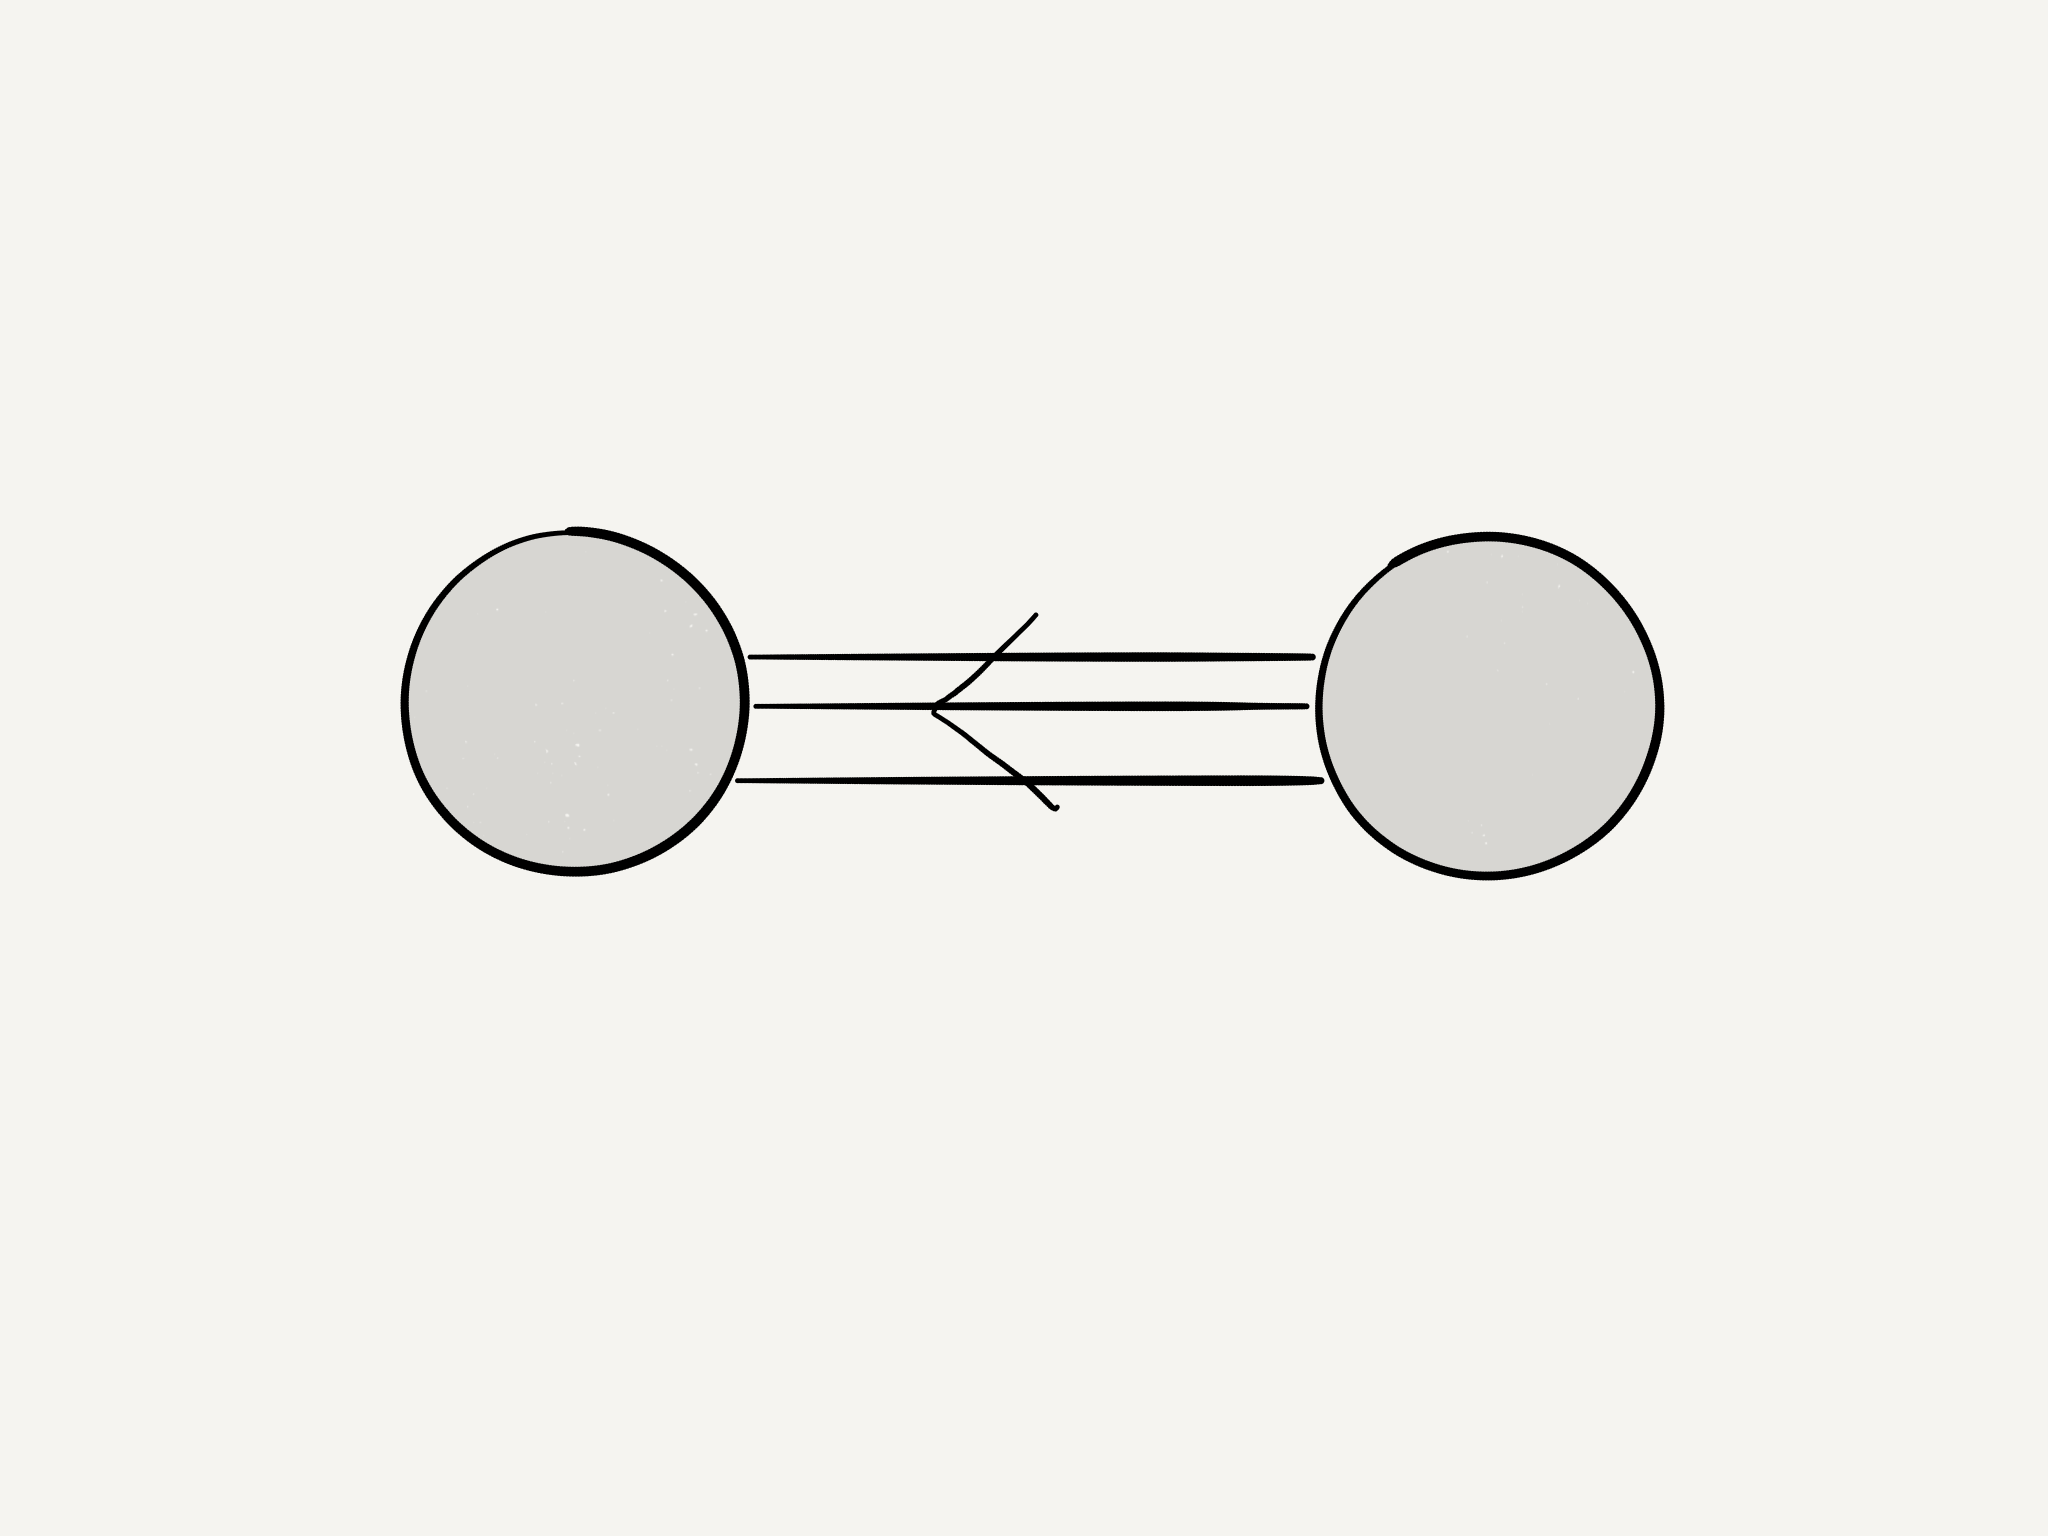
\includegraphics[scale=.2]{249-27.png}
\]

Suppose to the contrary that $_k \Phi = \Phi(G, S)$ has rank 1 (so it is A$_1$ or BC$_1$, but we do not need that). 
There are no nontrivial diagram isomorphisms, so the $\ast$-action must be trivial. Hence, 
$\Delta_0$ is one of the two vertices and the other restricts on $S$ 
to give the unique vertex in $_k \Delta$. Since there are no diagram automorphisms
and G$_2$ has trivial center, so G$_2$ is its own automorphism scheme, the $k$-group $G$ is classified
by an element $[G] \in {\rm{H}}^1(k, {\rm{G}}_2)$.  We will prove that $[G]$ is trivial by performing
reduction of the structure group (guided by such reduction steps in the proof
of the Relative Isomorphism Theorem). 

Let $c \in \Delta$ be the vertex not in $\Delta_0$.  (If we label the absolute diagram
with $a$ as the long root and $b$ as the short root then necessarily $c = a$ because if $c = b$ then
the highest absolute root $2a + 3b$ for G$_2$ would restrict to $3c|_S$, an absurdity since
roots are never multipliable by 3 in a root system. But it does not matter for the argument 
that we can identify this restriction on $c$.) The minimal parabolic $k$-subgroup
of $G$ corresponding to ${}_k\Delta$ therefore corresponds to the standard
parabolic $k$-subgroup $P = {}_k P_c \subset {\rm{G}}_2$. 

 The Galois-twisting by points in G$_2(k_s)$
that builds $G$ from the split group G$_2$ therefore can be given by conjugation
against points in G$_2(k_s)$ that normalize $P_{k_s}$.  
By Chevalley's Theorem from the first day of the course, $P(k_s)$
is the normalizer of $P_{k_s}$ inside G$_2(k_s)$. Hence, 
the 1-cocycle for $G$ can be arranged to be valued in $P_c(k_s)$,
which is to say $[G]$ comes from ${\rm{H}}^1(k, P_c)$.  That provides a first reduction of the structure group.
A second reduction is achieved by:

\begin{lemma} Let $P$ be a parabolic $k$-subgroup in a connected reductive
$k$-group, with $U = \mathscr{R}_{u,k}(P)$.
For any Levi $k$-subgroup $L \subset P$, the natural map
${\rm{H}}^1(k, L) \rightarrow {\rm{H}}^1(k, P)$ is bijective.
\end{lemma}

\begin{proof}
Identifying $L$ with $P/U$ provides a natural map
$$f:{\rm{H}}^1(k, P) \rightarrow {\rm{H}}^1(k, L)$$
that is surjective (using ${\rm{H}}^1(k, L) \rightarrow {\rm{H}}^1(k, P)$
arising from the inclusion of $L$ into $P$).  We will show that $f$ is actually
bijective, from which the desired result is then immediate.

The technique of twisting by torsors (cocycle-twisting in more classical language)
implies that all elements of the fiber of $f$ through a $P$-torsor $\xi$
arise from ${\rm{H}}^1(k, U_{\xi})$ for a certain Galois-twisted form $U_{\xi}$ of $U$.
But whether or not a smooth connected unipotent $k$-group is $k$-split
is {\em unaffected} by separable extension of the ground field (this is part of
Tits' structure theorem for unipotent groups; see the compatibility
with separable extension at the end of Theorem \ref{IV.4.2}). Thus, 
since $(U_{\xi})_{k_s} \simeq U_{k_s}$ is $k_s$-split, it follows that
$U_{\xi}$ is $k$-split. Hence, $U_{\xi}$ has a composition series whose successive
quotients are vector groups over $k$, so ${\rm{H}}^1(k, U_{\xi}) = 1$.  This implies that
the surjective $f$ has singleton fibers and so is bijective as claimed. 
\end{proof}

Now we know that $[G]$ arises
from ${\rm{H}}^1(k, L_c)$ for a Levi $k$-subgroup $L_c$ of $P_c$.
Note that $L_c$ is split  (we are working inside the split G$_2$, after all),
and it has root system with basis $\{c\}$ of size 1.  Since
$L_c$ is split, the quotient torus $L_c/\mathscr{D}(L_c)$ is a split torus
and so has vanishing H$^1$ by Hilbert 90.  Thus, the natural map
${\rm{H}}^1(k, \mathscr{D}(L_c)) \rightarrow {\rm{H}}^1(k, L_c)$ is surjective,
so we achieve yet another reduction of the structure group:
$[G]$ arises from ${\rm{H}}^1(k, \mathscr{D}(L_c))$.

But what is $\mathscr{D}(L_c)$?  This is a split connected semisimple group of rank 1,
so it is either SL$_2$ or PGL$_2$.  In fact, it must be SL$_2$.   This could be seen
by a direct argument with root groups, but here is a reason based on general principles
applicable more widely: 
Levi subgroups of parabolic subgroups are always given by 
torus centralizers (these always arises as $Z_G(\lambda)$), 
and in a connected semisimple group that is simply connected
the derived group of any torus centralizer
is always simply connected by Corollary \ref{levisc}!   Since G$_2$ is simply connected, that rules out PGL$_2$
and so $\mathscr{D}(L_c) = {\rm{SL}}_2$.  But
${\rm{H}}^1(k, \SL_n) = 1$ for any $n \ge 2$ due to the exact sequence of pointed sets
$${\rm{GL}}_n(k) \stackrel{\det}{\rightarrow} k^{\times} \stackrel{\delta}{\rightarrow}
{\rm{H}}^1(k, \SL_n) \rightarrow {\rm{H}}^1(k, \GL_n)$$
along with the surjectivity of the determinant and the vanishing of ${\rm{H}}^1(k, \GL_n)$
(as all vector bundles on ${\rm{Spec}}(k)$ are free!).  Thus,
${\rm{H}}^1(k, \SL_2) = 1$, so we are done.
\end{example}

The moral is that the classification of forms involves systematic reduction of the structure group. 

\newpage

\appendix

\section{Lang's theorem and dynamic methods}\label{langdyn}

In the previous course, we punted to \cite[\S16]{Borel} for Lang's technique on how
to establish certain results for {\em connected} linear algebraic groups over finite fields
that are proved over infinite fields via Zariski-density considerations with rational points
(as cannot work over a finite field).  This appendix gives  a complete treatment
of Lang's theorem, along with some important applications (filling in the case of finite fields
for Grothendieck's theorem on geometrically maximal tori).  We also review 
dynamic techniques, complementing those worked out in HW10
of the previous course, to prove the absolutely essential fact that a torus centralizer
in a connected linear algebraic group is not only smooth but especially {\em connected};
this underlies a vast range of arguments that proceed via dimension induction,
such as the proof of Chevalley's all-important self-normalizing property of parabolic
subgroups of connected linear algebraic groups (shown in the first lecture).

\subsection{Lang's theorem}

The following result of Lang is useful to circumvent the absence of Zariski-density techniques 
with rational points in the study of 
{\em connected} linear algebraic groups over finite fields:

\begin{theorem}[Lang]\label{langthm} Let $G$ be a connected group scheme of finite type over a finite field $k$, and
let $X$ be a non-empty finite type $k$-scheme equipped with a left $G$-action $G \times X \rightarrow X$ such that
$G(\overline{k})$ acts transitively on $X(\overline{k})$.  Then $X(k)$ is non-empty.
\end{theorem}

Lang's theorem is stated and proved in \cite[\S16]{Borel} in the affine setting,
but the proof works without affineness and so we will proceed in that generality.  

In practice, Lang's theorem is often applied to a special class of $X$, 
namely $G$-torsors.  The torsor property is the condition that the action is ``simply transitive''.
To be precise, if $H$ is a group scheme of finite type over a field $K$
and $E$ is a finite type $K$-scheme equipped with a left $H$-action then 
$E$ is an {\em $H$-torsor} (for the fppf topology) if the natural map
$$H \times E \rightarrow E \times E$$
defined by $(h,x) \mapsto (h.x, x)$ is an isomorphism.
The techniques of descent theory imply that in such cases, $E$ inherits
many ``nice'' properties of $H$ (smoothness, properness, geometric connectedness, etc.).
In case $H$ is smooth, such an $E$ is necessarily smooth and so $E(K_s)$ is non-empty;
we then say $E$ is a torsor for the \'etale topology (over $K$).  

\begin{example} A typical source of $H$-torsors is fibers over $K$-points
for the faithfully flat quotient map $G \rightarrow H\backslash G$ with a finite type $K$-group scheme
$G$ containing $H$ as a closed $K$-subgroup scheme, especially when $G$ is smooth
(and $H$ is often but not always smooth).  Lang's theorem
is the key tool to use for lifting rational points of
$H \backslash G$ to rational points of $G$ when working over a finite field,
in the presence of connectedness of $H$.  
Such connectedness is an essential assumption, as we see by trying to lift $k$-rational points to
$k$-rational points through 
the quotient map ${\rm{GL}}_1 \rightarrow {\rm{GL}}_1$ defined by
$t \mapsto t^n$ for an integer $n > 1$ (using $H = \mu_n$). 
\end{example}

To prove Lang's theorem, first observe that 
since $X$ is non-empty, we may and do choose $x_0 \in X(\overline{k})$.
We seek a $k$-point in $X$, and over $\overline{k}$ such a point must have 
the form $g_0(x_0)$ for some $g_0 \in G(\overline{k})$.   For any $k$-scheme $Z$,
denote the $q$-Frobenius morphism $F_{Z/k,q}:Z \rightarrow Z$ over $k$ by
the notation $z \mapsto z^{[q]}$ functorially on points.
(Note that $F_{Z/k,q}$ is functorial in $Z$ over $k$.)
This is the identity on the underlying topological space and the $q$-power endomorphism
of the structure sheaf.  
The $k$-rationality of a point $g_0(x_0) \in X(\overline{k})$
amounts to the ``Galois-invariance'' property 
$g_0(x_0)^{[q]} =  g_0(x_0)$.  

The $G$-action on $X$ is defined over
$k$, so 
$$g_0(x_0)^{[q]} = (g_0)^{[q]}(x_0^{[q]}).$$
Hence, we can recast our problem is that of finding $g_0 \in G(\overline{k})$ such that
$$(g_0^{-1} \cdot (g_0)^{[q]})(x_0^{[q]}) = x_0.$$
Since the $G(\overline{k})$-action on $X(\overline{k})$ is transitive by hypothesis,
$x_0^{[q]} = g'(x_0)$ for some $g' \in G(\overline{k})$.  Thus, 
it suffices to show that for any $g' \in G(\overline{k})$,
${g'}^{-1}$ has the form $g_0^{-1} \cdot (g_0)^{[q]}$ for some $g_0 \in G(\overline{k})$,
or equivalently $g' = (g_0^{-1})^{[q]} \cdot g_0$.
In other words, we are reduced to proving that 
the $k$-scheme morphism $L:G \rightarrow G$ defined by $$L(g) = g^{[q]} \cdot g^{-1}$$
is surjective on $\overline{k}$-points (or equivalently, is a surjective map of $k$-schemes, 
as $G$ is finite type over $k$). In the special case $G = \mathbf{G}_{\rm{a}}$
this is the Artin-Schreier map $t \mapsto t^q - t$, so
the map $L$ is a generalization
of the Artin-Schreier homomorphism; it is called the {\em Lang map}
(and is generally not a homomorphism when $G$ is non-commutative).  Our 
problem is now entirely about $G$ and has nothing anymore to do with $X$.

Since $k$ is perfect, $G_{\rm{red}}$ is a closed $k$-subgroup scheme of $G$ whose formation
commutes with any extension of the ground field, and it has the same $\overline{k}$-points as $G$. Thus, 
by functoriality of the $q$-Frobenius morphism with respect to the inclusion of $G_{\rm{red}}$
into $G$ we may replace $G$ with $G_{\rm{red}}$ so that $G$ is reduced
and hence smooth (as for any reduced group scheme of finite type over a perfect field).
Now we may use tangent space considerations to investigate the local structure of
$k$-morphisms from $G$ to itself.  

Consider the action of $G$ on itself via $g.x = g^{[q]} x g^{-1}$.
Clearly $L(G)$ is the orbit of the identity point.  To show that this is the only orbit
(and so $L$ is surjective),  by the connectedness
of $G$ and the disjointness of distinct orbits 
it is enough to prove that {\em every} $G$-orbit on $G_{\overline{k}}$ is
open.  To do this, it is enough to show that the
orbit map $g \mapsto g^{[q]} g_0 g^{-1}$ through every $g_0 \in G(\overline{k})$ is an open map.
We will show that all of these orbit maps $G \rightarrow G$ are \'etale.
By smoothness of $G$, it is equivalent to check that such orbit
maps are isomorphisms on tangent spaces at all points of the source.
The homogeneity of orbit maps
reduces this assertion to the isomorphism property
at a single point of $G(\overline{k})$, such as the identity point.

More specifically, the map $g \mapsto g^{[q]} g_0 g^{-1}$ carries $e$ to $g_0$
and we claim that the induced map ${\rm{T}}_e(G) \rightarrow {\rm{T}}_{g_0}(G)$ is an isomorphism.
It is harmless to post-compose with right translation by $g_0^{-1}$, so 
we are analyzing the map $f_{g_0}:g \mapsto L(g) \cdot (g g_0 g^{-1} g_0^{-1})$.
Recall the following differential identities:  the group law $m:G \times G \rightarrow G$ induces addition
${\rm{T}}_e(G) \oplus {\rm{T}}_e(G) \rightarrow {\rm{T}}_e(G)$,
inversion induces negation on ${\rm{T}}_e(G)$,
and $F_{G/k,q}$ induces the zero map on ${\rm{T}}_e(G)$.  Thus, 
${\rm{d}}L(e)$ is negation and so 
$${\rm{d}}f_{g_0}(e) = {\rm{d}}L(e) + {\rm{id}} - {\rm{Ad}}_G(g_0) = -{\rm{Ad}}_G(g_0).$$
Hence, ${\rm{d}}f_{g_0}(e)$ is an isomorphism, so 
$f_{g_0}$ is \'etale.  This proves that every $G$-orbit is open, so we are done.
In particular, the Lang map $L$ is an \'etale surjection.  In fact, we can do a bit better:

\begin{proposition} The fibers of $L$ are right $G(k)$-cosets inside $G$.  In particular, $L$ has {\em constant} fiber rank
$($namely, the size of $G(k)$$)$ over its open image $f(G)$.
\end{proposition}

\begin{proof} 
It suffices to check $L$ is \'etale on $G_{\overline{k}}$ at any $\overline{k}$-point
$g_0$, with each fiber $L^{-1}(L(g_0))$ a right $G(k)$-coset inside $G(\overline{k})$.
For the \'etale property of $L$ at $g_0$, it is equivalent to prove
the \'etale property of $g \mapsto L(g_0 g)$ at the identity.
But $$L(g_0g) = g_0^{[q]} (g^{[q]} g^{-1}) g_0^{-1} = g_0^{[q]} \cdot L(g) \cdot g_0^{-1}.$$
Since $L$ is \'etale at the identity, and 
post-composing with left translation by $g_0^{[q]}$ and right translation by
$g_0^{-1}$ amounts to applying automorphisms on the target, the desired
\'etaleness is established.

Analyzing the fibers amounts to an elementary computation:  
for $g, g_0 \in G(\overline{k})$, the equality $L(g) = L(g_0)$ says exactly that $g_0^{-1}g$ is fixed
by $F_{G/k,q}$ on $G(\overline{k})$.  But the set of such fixed points is exactly $G(k)$,
so $L(g) = L(g_0)$ if and only if $g_0^{-1}g \in G(k)$, which is to say
$g \in g_0 G(k)$.
\end{proof}

\begin{remark} By using Zariski's Main Theorem, one can show that a quasi-compact separated \'etale
map with constant fiber rank is necessarily {\em finite}, so $L:G \rightarrow G$ is not merely
surjective \'etale but even finite.  In fact, $L:g \mapsto g^{[q]} g^{-1}$ is visibly invariant
under the right $G(k)$-action on $G$, so $L$ actually exhibits $G$ as a right $G(k)$-torsor over itself.
For commutative $G$, the map $L$ is usually called the {\em Lang isogeny}.
\end{remark}

Lang's theorem has very useful consequences.  We record the most basic one here:

\begin{lemma}\label{corlang} Let $G$ be a smooth connected affine group over a finite field $k$.
There exists a $k$-torus $T \subset G$ that is maximal over
$\overline{k}$ and there exists a Borel $k$-subgroup $B \subset G$.
\end{lemma}

The proof (in the previous course) of Grothendieck's theorem on the existence of (geometrically!) maximal tori over
the ground field was carried out almost entirely over infinite fields via Zariski-density considerations
with ``rational points'' in Lie algebras over the ground field.  The case of finite fields
was punted to Lang's theorem via exactly the torus part of Corollary \ref{corlang}, so that fills in the loose
end for the treatment of finite fields in the proof of Grothendieck's theorem.

The right proof of Corollary \ref{corlang} is to construct moduli schemes
${\rm{Tor}}_{G/k}$ and ${\rm{Bor}}_{G/k}$ 
whose sets of rational points over any extension $k'/k$ are respectively naturally identified
with the sets of geometrically maximal $k'$-tori and of Borel $k'$-subgroups, 
and to apply Lang's theorem with $X$ taken to be either of these moduli schemes
(equipped with the natural {\em transitive} $G$-action via conjugation). 
To be precise, over an arbitrary field $k$ there exist closed subschemes
$$\mathscr{T} \subset G \times {\rm{Tor}}_{G/k},\,\,\,
\mathscr{B} \subset G \times {\rm{Bor}}_{G/k}$$
that respectively represent functors of maximal tori and Borel subgroups
in a relative setting, or in a weaker (but sufficient) sense recover
exactly the geometrically maximal $k'$-tori and the Borel $k'$-subgroups
as we vary through all $k'$-point fibers of
$\mathscr{T} \rightarrow {\rm{Tor}}_{G/k}$
and $\mathscr{B} \rightarrow {\rm{Bor}}_{G/k}$ 
inside $G_{k'}$ with any extension field $k'/k$.   

For our purposes,
rather than construct such moduli schemes (which is a game of Galois descent
for perfect ground fields, and very delicate over imperfect
fields), we will instead adapt the {\em method} of proof of Lang's theorem rather
than apply the {\em statement} of the theorem.

\begin{proof}
We give the argument for geometrically maximal tori, and the case of Borel subgroups 
goes similarly. Pick a maximal torus $T' \subset G_{\overline{k}}$,
so we seek $g \in G(\overline{k})$ such that $gT' g^{-1}$ is ${\rm{Gal}}(\overline{k}/k)$-invariant.
That is, if $k$ has size $q$ then we want $F_{G/k,q}(gT'g^{-1}) = gT' g^{-1}$.
This says that $(g^{[q]})^{-1}g T' g^{-1} g^{[q]} = {T'}^{[q]}$.
Since ${T'}^{[q]}$ and $T'$ are maximal tori in $G_{\overline{k}}$,
by the conjugacy of maximal tori over $\overline{k}$ there
exists $g' \in G(\overline{k})$ such that $g' T' {g'}^{-1} = {T'}^{[q]}$.
Hence, it suffices to find $g \in G(\overline{k})$ such that
$(g^{[q]})^{-1} g = g'$.  This says that the Lang map $L:G \rightarrow G$
carries $g^{-1}$ onto $g'$.  Since the Lang map is surjective, we are done.
\end{proof}


\subsection{Subgroups associated to a 1-parameter subgroup}

For a field $k$, let $G$ be a smooth affine $k$-group, and $\lambda:\mathbf{G}_m
\rightarrow G$ a $k$-homomorphism (possibly trivial, though that case is not
interesting). One often calls $\lambda$ a {\em $1$-parameter $k$-subgroup} of $G$,
even when $\ker \lambda \ne 1$.  Such a homomorphism 
defines a left action of $\mathbf{G}_m$ on $G$ via
the functorial procedure $t.g = \lambda(t)g\lambda(t)^{-1}$ for
$g \in G(R)$ and $t \in R^{\times}$ for any $k$-algebra $R$. In class (see \S\ref{ztorconn}) we introduced the following 
subgroup functors of $G$:  for any $k$-algebra $R$,
$$P_G(\lambda)(R) = \{g \in G(R)\,|\,\lim_{t \rightarrow 0} t.g \mbox{ exists }\},\,\,\,
U_G(\lambda)(R) = \{g \in G(R)\,|\,\lim_{t \rightarrow 0} t.g = 1\},$$
and 
$$Z_G(\lambda)(R) = \{g \in G(R)\,|\,\lambda_R \mbox{ centralizes } g\}.$$
In the March 10 lecture of the previous course it was proved that these are all represented by closed $k$-subgroup schemes of $G$,
with $P_G(\lambda) = Z_G(\lambda) \ltimes U_G(\lambda)$.  

By a direct calculation with graded modules over the dual numbers, it is shown in \cite[Prop.\,2.1.8(1)]{pred}
that when using the $\Z$-grading $\oplus_{n \in \Z} \mathfrak{g}_n$ of $\mathfrak{g} = {\rm{Lie}}(G)$
defined by the $\mathbf{G}_m$-action induced by conjugation through $\lambda$ (i.e., $\mathfrak{g}_n$ is
the space of $v \in \mathfrak{g}_n$ such that ${\rm{Ad}}_G(\lambda(t))(v) = t^n v$ for all $t \in \mathbf{G}_m$), we have
$${\rm{Lie}}(Z_G(\lambda)) = \mathfrak{g}_0,\,\,\,
{\rm{Lie}}(U_G(\lambda)) = \mathfrak{g}^+ := \bigoplus_{n > 0} \mathfrak{g}_n.$$
For example, if $T \subset G$ is a split $k$-torus and $\lambda$ is valued in $T$, then using the resulting
$T$-weight space decomposition $\mathfrak{g} = {\rm{Lie}}(Z_G(T)) \oplus (\oplus_{a \in \Phi} \mathfrak{g}_a)$
(with $\Phi$ the set of nontrivial $T$-weights on $\mathfrak{g}$) we see that for any
$n \in \Z - \{0\}$,
$$\mathfrak{g}_n = \bigoplus_{\langle a, \lambda \rangle = n} \mathfrak{g}_a$$
since the adjoint action of $\lambda(t)$ on $\mathfrak{g}_a$ is multiplication by
$a(\lambda(t)) = t^{\langle a, \lambda \rangle}$.  Hence, 
$$\mathfrak{g}_0 = {\rm{Lie}}(Z_G(T)) \oplus (\oplus_{\langle a, \lambda \rangle = 0} \mathfrak{g}_a),\,\,\,
{\rm{Lie}}(U_G(\lambda)) = \mathfrak{g}_+ = \oplus_{\langle a, \lambda \rangle > 0} \mathfrak{g}_a.$$


We write $\lambda^{-1}$ to denote the reciprocal homomorphism $t \mapsto \lambda(t)^{-1} = 
\lambda(1/t)$. 
In Exercise 3 of HW10 of the previous course you were led through a direct 
 proof that if $G = {\rm{GL}}(V)$ then the multiplication map
$$\mu = \mu_{G,\lambda}:U_G(\lambda^{-1}) \times P_G(\lambda) \rightarrow G$$
is an open immersion, with $P_G(\lambda)$ a subgroup of ``block upper-triangular matrices''
and $U_G(\lambda)$ its unipotent radical (even over $\overline{k}$).  We first wish to 
deduce the open immersion property for {\em general} $G$ from that special case, which immediately implies:

\begin{lemma} The $k$-groups $U_G(\lambda)$,
$P_G(\lambda)$, and $Z_G(\lambda)$ are all smooth, and all 
 are connected when $G$ is connected.  Likewise, $U_G(\lambda)$
 is unipotent in general.
 \end{lemma}
 
 Indeed, the inheritance of smoothness and connectedness by direct factors gives the first
 assertion of this corollary, and the final assertion is immediate via 
functoriality with respect to an inclusion
 $G \hookrightarrow {\rm{GL}}_n$ (as that reduces it to the settled case
 of ${\rm{GL}}_n$).  Note that by iterating the connectedness of $Z_G(\lambda)$ several times (using
$\lambda$'s that generate a given torus in $G_{\overline{k}}$) we obtain the important:

\begin{lemma} If $G$ is a connected linear algebraic group then 
$Z_G(S)$ is smooth and connected for any $k$-torus $S$ in $G$. 
\end{lemma}

To establish the open immersion property for $\mu$
in general, consider any pair $(G,\lambda)$ and a $k$-subgroup inclusion $j:G \hookrightarrow G'$ into
another smooth affine $k$-group (the case of interest being $G' = {\rm{GL}}(V)$).
Let $\lambda' = j \circ \lambda$.
By the functorial definition, 
$$P_G(\lambda) = G \cap P_{G'}(\lambda'), U_G(\lambda^{\pm 1}) = G \cap
U_{G'}({\lambda'}^{\pm 1}), Z_G(\lambda) = G \cap Z_{G'}(\lambda').$$
In particular, if $U_{G'}({\lambda'}^{-1}) \cap P_{G'}(\lambda') = 1$
then $U_G(\lambda^{-1}) \cap P_G(\lambda) = 1$.  In other words,
if $\mu' = \mu_{G',\lambda'}$ is a monomorphism then so is $\mu$.
This monicity hypothesis on $\mu$ for $G' = {\rm{GL}}(V)$ (and any $1$-parameter
$k$-subgroup $\lambda'$ of ${\rm{GL}}(V)$) was verified in HW10 of the previous course, so 
$\mu$ is monic in general.  But is it an open immersion?

If $\mu'$ is an open immersion (as is proved on HW10 from the previous course for $G' = {\rm{GL}}(V)$!)
then the same holds for $\mu$ due to the following non-obvious lemma:

\begin{lemma}\label{rholine} With notation as above, if $\mu'$ is monic then
$$G \cap (U_{G'}({\lambda'}^{-1}) \times P_{G'}(\lambda')) = U_G(\lambda^{-1}) \times
P_G(\lambda)$$
as subfunctors of $G$.
\end{lemma}

\begin{proof}
Since $P_{G'}(\lambda') = U_{G'}(\lambda') \rtimes Z_{G'}(\lambda')$,
by evaluating on points valued in $k$-algebras $R$ we have to show that if
$$u'_{-} \in U_{G'}({\lambda'}^{-1})(R), \,\,\,
u'_{+} \in U_{G'}(\lambda')(R), \,\,\, z' \in Z_{G'}(\lambda')(R)$$ and 
$u'_{-}u'_{+} z'= g \in G(R)$ then 
that $u'_{+}, u'_{-}, z' \in G(R)$. 

As usual, we can pick a finite-dimensional $k$-vector space $V$,
a $k$-homomorphism $\rho:G' \rightarrow {\rm{GL}}(V)$, and a line
$L$ in $V$ such that $G$ is the scheme-theoretic stabilizer of $L$ in $G'$.  
Let $v \in L$ be a basis element, so $\rho(g)(v) = cv$ in $V_R = R \otimes_k V$ for a unique $c \in R^{\times}$.  
Since $g = u'_{-} u'_{+} z'$, we get 
\begin{equation}\label{rhocv}
\rho(u'_{+}z')(v) = c \rho((u'_{-})^{-1})(v)
\end{equation} 
in $V_R$.  

For any point $t$ of $\mathbf{G}_m$ valued in an $R$-algebra $R'$, the point 
$\lambda'(t)$ of $G'(R')$ lies in $G(R')$ 
and so acts on $v$ (through $\rho$) by some ${R'}^{\times}$-scaling.  Hence, we can replace
$v$ with $\rho(\lambda'(t)^{-1})(v)$ on both sides of (\ref{rhocv}).  
Now act on both sides
of (\ref{rhocv}) by $\rho(\lambda'(t))$, and then 
commute $\rho(\lambda'(t)^{-1})$ past $\rho(z')$ (as we may, since $z' \in Z_{G'}(\lambda')(R)$) to get the identity
\begin{equation}\label{tuzid}
\rho((t.u'_{+})z')(v) = c \rho(t.(u'_{-})^{-1})(v)
\end{equation} 
as points of the affine space $\underline{V}_R$ over $R$ covariantly associated to $V_R$.

Viewing the two sides of (\ref{tuzid}) as $R$-scheme maps $(\mathbf{G}_m)_{R} \rightarrow \underline{V}_{R}$,
the left side extends to an $R$-map $\mathbf{P}^1_R - \{\infty\} = \mathbf{A}^1_R \rightarrow 
\underline{V}_R$
and the right side extends to an $R$-map $\mathbf{P}^1_R - \{0\} \rightarrow \underline{V}_R$.  By 
combining these, we arrive at an $R$-map $\mathbf{P}^1_R \rightarrow \underline{V}_R$ from the projective
line to an affine space over $R$.  The only such map is a constant $R$-map to some $v_0 \in 
\underline{V}_R(R) = V_R$ (concretely, $R[t] \cap R[1/t] = R$ inside of $R[t,1/t]$), 
so both sides of (\ref{tuzid}) are independent of $t$ (and equal to $v_0$).  
Passing to the limit as $t \rightarrow 0$ on the left side and as $t \rightarrow \infty$ on the right side
yields $\rho(z')(v) = v_0 = c v$.    
We have proved that $z'$ carries $v$ to an $R^{\times}$-multiple
of itself.  Thus, the point $z' \in G'(R)$ is an $R$-point of the functorial stabilizer of $L$ inside of $V$.    
This stabilizer is
exactly $G$, by the way we chose $\rho$, so $z'$ is an $R$-point of $G \cap Z_{G'}(\lambda') = Z_G(\lambda)$. 

Since $\rho(z')(v) = cv$, by cancellation of $c$ on both sides of 
the identity (\ref{tuzid}) we get $$\rho(t.u'_{+})(v) = \rho(t.(u'_{-})^{-1})(v)$$ with both sides
independent of $t$ and equal to $c^{-1} v_0 = v$.  Taking $t = 1$, this says that $u'_{\pm}$ lies
in the stabilizer $G$ of $v$, so $u'_{\pm}$ is an $R$-point of $G \cap U_{G'}({\lambda'}^{\pm 1}) = 
U_G(\lambda^{\pm 1})$,
as required.  
\end{proof}

At the end of the March 10 lecture of the previous course,
we used the open immersion property for $\mu$ to prove the following crucial result:

\begin{proposition}\label{puzsurj}
Let $f:G \twoheadrightarrow G'$ be a surjective $k$-homomorphism between smooth
connected affine $k$-groups, and let $\lambda:\mathbf{G}_m \rightarrow G$ be
a $k$-homomorphism.  For $\lambda' = f \circ \lambda$, the natural maps
$P_G(\lambda) \rightarrow P_{G'}(\lambda')$,
$U_{G}(\lambda) \rightarrow U_{G'}(\lambda')$,
and $Z_G(\lambda) \rightarrow Z_{G'}(\lambda')$ are surjective.
\end{proposition}

We have shown that surjective homomorphisms between smooth connected
affine $k$-groups carry maximal $k$-tori onto maximal $k$-tori and Borel $k$-subgroups
onto Borel $k$-subgroups.  Another related important compatibility is the good behavior of
{\em torus centralizers} under surjective homomorphisms.  This follows from the preceding proposition:

\begin{lemma}\label{zimage} Let $f:G \twoheadrightarrow G'$ be a surjective $k$-homomorphism between
smooth connected affine $k$-groups. Let $S$ be a $k$-torus in $G$,
and $S' = f(S)$. Then $f(Z_G(S)) = Z_{G'}(S')$.
\end{lemma}

This result is  \cite[11.14, Cor.\,2]{Borel}.  You may find it instructive to compare the proofs. 

\begin{proof}
We may assume $k = \overline{k}$.  If $S_1$ and $S_2$ are $k$-subtori in $S$
such that $S_1 \cdot S_2 = S$, which is to say that the $k$-homomorphism
$S_1 \times S_2 \rightarrow S$ is surjective, it is an exercise (do it!)
to check that $Z_G(S) = Z_{Z_G(S_1)}(S_2)$.  (Note that since torus centralizers in smooth
affine groups are smooth, this equality may be checked by computing with geometric points.) 
Hence, by induction on
$\dim S$, we may and do assume $S \simeq \mathbf{G}_m$.

With $S \simeq \mathbf{G}_m$, the inclusion of $S$ into $G$ is given by a $k$-homomorphism
$\lambda:\mathbf{G}_m \rightarrow G$ with image $S$.
Likewise, $\lambda' = f \circ \lambda:\mathbf{G}_m \rightarrow G'$ has image $S'$.
Hence, $Z_G(S) = Z_G(\lambda)$ and $Z_{G'}(S') = Z_{G'}(\lambda')$.
Thus, the map $Z_G(S) \rightarrow Z_{G'}(S')$ that we wish to prove is surjective
is identified with the natural map $Z_G(\lambda) \rightarrow Z_{G'}(\lambda')$.
By Proposition \ref{puzsurj}, this latter map is surjective!
\end{proof}

\subsection{Conjugacy for split tori}

It is a deep fact that in smooth connected affine groups $G$ over any field $k$, all 
maximal $k$-split $k$-tori $S$ in $G$ 
(not to be confused with $k$-split maximal $k$-tori, which may not exist!) are $G(k)$-conjugate.  
Their common dimension is called the {\em $k$-rank} of $G$; it could be considerably smaller
than the common dimension of the maximal $k$-tori (which may be called the {\em geometric rank},
since it is the $\overline{k}$-rank of $G_{\overline{k}}$).  

The proof of this $G(k)$-conjugacy 
rests on the case of reductive groups (and pseudo-reductive groups
when $k$ is imperfect), and we do not need it in general; in this course we will prove
it for reductive $G$.
The special case of ${\rm{PGL}}_2$ plays a role in getting the structure theory of reductive groups
off the ground, so we now give an elementary direct proof in the special case of
${\rm{PGL}}_n$ and ${\rm{GL}}_n$:


\begin{proposition} Let $V$ be a finite-dimensional vector space over a field,
and $G = {\rm{GL}}(V)$ or ${\rm{PGL}}(V)$.  The maximal $k$-split $k$-tori in $G$
are $G(k)$-conjugate to each other.  
\end{proposition}

\begin{proof}
The quotient map ${\rm{GL}}(V) \rightarrow {\rm{PGL}}(V)$ has kernel
$\mathbf{G}_m$ and is surjective on $k$-points (!), so it is easy to reduce to the case of
${\rm{GL}}(V)$ in place of ${\rm{PGL}}(V)$ (check!).  By  HW5, Exercise 5 of the previous course, such $k$-tori
correspond precisely to commutative $k$-subalgebras $A \subseteq {\rm{End}}(V)$ of
the form $A \simeq k^n$ with $n = \dim V$.  Such a $k$-subalgebra amounts to a $k^n$-module
structure on an $n$-dimensional vector space $V$, which is nothing more or less than a decomposition
of $V$ into a direct sum of lines.  But any two such decompositions are clearly related via the action of
${\rm{Aut}}_k(V) = {\rm{GL}}(V)(k)$, so we are done.  
\end{proof}

Now we turn out attention to an ``axiomatic'' $G(k)$-conjugacy result.  The axioms turn out to hold for
all connected reductive $k$-groups containing a split maximal $k$-torus, as we will show later
(see Remark \ref{ver}), but we note here that it will rest on the dynamic method (which is why we mention
the topic in this appendix, to illustrate how useful the dynamic viewpoint is).

\begin{theorem}\label{axiom} Let $G$ be a smooth connected affine $k$-group such that 
for every maximal torus $T$ in $G_{\overline{k}}$, $Z_{G_{\overline{k}}}(T) = T$
and the finite group $W_{G_{\overline{k}}}(T)$ acts transitively on
the set of Borel subgroups of $G_{\overline{k}}$ containing $T$.  Also assume
that any Borel subgroup $B$ of $G_{\overline{k}}$ satisfies $N_{G(\overline{k})}(B) = B(\overline{k})$.
 
 Assume that $G$ contains a $k$-split maximal $k$-torus, and
 that for all such $k$-tori $T$ 
there is a Borel $k$-subgroup $B$ containing $T$.  All such pairs $(T, B)$ are $G(k)$-conjugate to each other.
\end{theorem}

The centralizer hypothesis on the maximal tori of $G_{\overline{k}}$ is invariant under
conjugation, so by the $G(\overline{k})$-conjugacy of all maximal tori of $G_{\overline{k}}$
it suffices to check this condition for one maximal torus of $G_{\overline{k}}$.  The same
holds for the normalizer hypothesis on Borel subgroups.

\begin{remark}
In the homework for the previous course we have seen many examples of $G$ for which $Z_G(T) = T$ for some
maximal $k$-torus $T$, such as ${\rm{GL}}_n$, ${\rm{SL}}_n$, ${\rm{Sp}}_{2n}$,
and ${\rm{SO}}_n$ with their ``diagonal''  (split) maximal $k$-tori.   But don't forget that there
are plenty of interesting nontrivial $k$-anisotropic connected reductive groups,
such as ${\rm{SL}}(D)$ for a finite-dimensional central division algebra $D \ne k$ and
${\rm{SO}}(q)$ for an anisotropic quadratic space $(V,q)$ over $k$ with $\dim V \ge 3$,
and in such cases there is {\em no nontrivial $k$-split torus} at all, let alone one which is maximal
as a $k$-torus. 
\end{remark}

\begin{remark}\label{ver}
 It is a general fact that $Z_G(T) = T$ for {\em every} maximal torus $T$ in any connected
reductive group $G$, but this is not at all obvious from the definitions; it will be proved later 
as part of a general development of basic structure theory of connected reductive groups.
Likewise, the general development will verify the transitivity axiom on Weyl groups in Theorem \ref{axiom} for connected reductive groups,
as well as the fact that any $k$-split maximal $k$-torus (if one exists!) in a connected
reductive $k$-group lies in a Borel $k$-subgroup. 
Finally, the self-normalizing
property of Borel subgroups is a fundamental result of Chevalley for any smooth connected
affine $\overline{k}$-group, as mentioned at the start of this appendix.
\end{remark}

To begin the proof of Theorem \ref{axiom}, 
let $T$ and $T'$ be $k$-split maximal $k$-tori in $G$, and choose
Borel $k$-subgroups $B \supset T$ and $B' \supset T'$.  We have $T = Z_G(T)$ and $T' = Z_G(T')$, 
since such equality among $k$-subgroups may be checked over $\overline{k}$
(where it follows from the hypotheses).   
The proof goes in two steps:  conjugacy over $k_s$, and then a Galois cohomology argument to
get down to $k$.  But we follow the usual ``reduction step'' style and argue in reverse,
by first showing that the general case can be reduced to the separably closed case,
and then handling the case $k = k_s$. 

Let's first reduce to the case of maximal tori over separably closed $k$:  we will prove that if
$T_{k_s}$ and $T'_{k_s}$ are $G(k_s)$-conjugate then they are $G(k)$-conjugate
by an element carrying $B_{k_s}$ to $B'_{k_s}$.
Pick $g \in G(k_s)$ such that $T'_{k_s} = g T_{k_s} g^{-1}$, so
$g B_{k_s} g^{-1}$ and $B'_{k_s}$ are Borel $k_s$-subgroups containing
$T'_{k_s}$.  We first seek to choose $g$ so that also these Borel $k_s$-subgroups coincide.

By hypothesis, the group $W_{G_{\overline{k}}}(T'_{\overline{k}})$ acts
transitively on the set of Borel $\overline{k}$-subgroups containing
$T'_{\overline{k}}$.  But $W_G(T')$ is a finite \'etale $k$-group, so its geometric points
are defined over $k_s$.  Thus, 
$$N_G(T')(k_s)/T'(k_s) = W_G(T')(k_s) = W_G(T')(\overline{k}) =W_{G_{\overline{k}}}(T'_{\overline{k}}).$$
In other words, the group $N_G(T')(k_s) = N_{G(k_s)}(T'_{k_s})$ acts
transitively on the set of Borel $\overline{k}$-subgroups of $G_{\overline{k}}$ containing $T'_{\overline{k}}$.
Hence, replacing $g \in G(k_s)$ with its left-translate by some element of $N_G(T')(k_s)$
(which doesn't affect the condition that $gT_{k_s} g^{-1} = T'_{k_s}$!)
brings us to the case that the Borel $k_s$-subgroups $gB_{k_s}g^{-1}$ and $B'_{k_s}$
containing $T'_{k_s}$ coincide over $\overline{k}$ and hence coincide over $k_s$.

Now we use a Galois cohomology argument to push down
the $G(k_s)$-conjugacy to $G(k)$-conjugacy.
For any $\gamma \in {\rm{Gal}}(k_s/k)$ we apply $\gamma$ to both sides of the equalities
$$T'_{k_s} = g T_{k_s} g^{-1},\,\,\,B'_{k_s} = g B_{k_s} g^{-1}.$$
This gives 
$$T'_{k_s} = \gamma(g) T_{k_s} \gamma(g)^{-1},\,\,\,
B'_{k_s} = \gamma(g) B_{k_s} \gamma(g)^{-1},$$ 
so $\gamma(g)^{-1}g$ normalizes $T_{k_s}$ as well as $B_{k_s}$.
By hypothesis $N_{G(\overline{k})}(B_{\overline{k}}) = B(\overline{k})$,
so $$\gamma(g)^{-1}g \in B(\overline{k}) \cap G(k_s) = B(k_s)$$
and likewise $\gamma(g)^{-1}g \in N_G(T)(k_s)$.

If we did not have available the Borel $k$-subgroups
and only worked with the split maximal $k$-tori, we would only have
$\gamma(g)^{-1}g \in N_G(T)(k_s)$ and then we would get hopelessly stuck
due to possible obstructions in ${\rm{H}}^1(k_s/k, W_G(T))$.
Now the importance of using the Borel $k$-subgroups
emerges:  $B(k_s) \cap N_G(T)(k_s) = T(k_s)$!  Indeed, since $T = Z_G(T)$ (by our hypotheses) we can express this as the statement that
$N_B(T)(k_s) = Z_B(T)(k_s)$, and this in turn is a special case of:

\begin{lemma} Let $H$ be a connected solvable smooth affine group over
a field $k$, and let $T$ be a maximal $k$-torus in $H$.  Then
$N_H(T)(k) = Z_H(T)(k)$.
\end{lemma}

\begin{proof}
Since $T_{\overline{k}}$ is a maximal torus in $H_{\overline{k}}$,
and the problem of showing a $k$-point of $H$ lies in the closed subset $Z_H(T)$
may be checked over $\overline{k}$, it is harmless to extend the ground
field to $\overline{k}$ so that $k$ is {\em algebraically closed}.
Hence, the structure theorem for connected solvable groups
becomes available:  $H = T \ltimes U$ for $U = \mathscr{R}_u(H)$.
To show that any $h \in H(k)$ normalizing $T$ actually centralizes $T$, we may assume
$h = u \in U(k)$.  Hence, for any $t \in T(k)$ we have
$$utu^{-1} = t(t^{-1}ut)u^{-1}.$$
But $(t^{-1}ut)u^{-1} \in U(k)$ since $U$ is normal in $H = T \ltimes U$, so
the condition that $utu^{-1} \in T(k)$ forces it to equal $t$.
\end{proof}

Thus, we have obtained a function $c:\gamma \mapsto \gamma(g)^{-1}g$ from ${\rm{Gal}}(k_s/k)$ to $T(k_s)$.
This functor factors through the quotient ${\rm{Gal}}(K/k)$ for a finite Galois extension $K/k$ inside of
$k_s$ such that $g \in G(K)$.  It is therefore easy to check that $c \in {\rm{Z}}^1(k_s/k, T(k_s))$. 
Consider the cohomology class $[c] \in {\rm{H}}^1(k_s/k,T)$.  Since $T \simeq \mathbf{G}_m^r$, this
cohomology group vanishes by Hilbert 90.  Hence, $c = \gamma(t)t^{-1}$ for some $t \in T(k_s)$.
Thus, if we replace $g$ with $gt$ (as we may!), we get to the case when $\gamma(g) = g$ for all $\gamma$,
so $g \in G(k)$.  That does the job.  (This idea adapts to pull down the result
from $\overline{k}$ by using Hilbert 90 for the fppf topology, but we give a more hands-on procedure below
to get down to $k_s$ from $\overline{k}$.) 

Now we can assume that $k = k_s$, and it remains to show:

\begin{proposition}\label{torsepconj} If $T$ and $T'$ are maximal tori in a smooth connected
affine group $G$ over a separably closed field $k$ then $T$ and $T'$ are $G(k)$-conjugate.
\end{proposition}

This says that the general conjugacy result over algebraically closed fields actually holds over separably
closed fields.  
I think it is due to Grothendieck.  Regardless, the argument we give is a version of the method he
used in \cite{SGA3} for smooth affine groups over any scheme (working locally for the \'etale topology). 
 The idea is similar to the trick with Isom-schemes in
HW4 Exercise 5 of the previous course.

\begin{proof}
Consider the functor $I$ on $k$-algebras defined by
$$I(R) = \{g \in G(R)\,|\,T'_R = gT_R g^{-1}\}.$$
This is a subfunctor of $G$, and its restriction 
$I_{\overline{k}}$ to $\overline{k}$-algebras is represented by a {\em smooth} closed
subscheme of $\overline{k}$:  since $T'_{\overline{k}} = g_0 T_{\overline{k}}  g_0^{-1}$ 
for some $g_0 \in G(\overline{k})$ by the known ``geometric'' case over $\overline{k}$, 
we see that $I_{\overline{k}}(R)$ consists of points $g \in G(R)$ such that $g_0^{-1}g \in Z_{G(R)}(T_R)$.
In other words, $I_{\overline{k}}$ is represented by $g_0 Z_G(T)_{\overline{k}}$.   By HW8, Exercise 3
of the previous course,
this is smooth and non-empty.  Thus, if we can prove that $I$ is represented by a closed
$k$-subscheme of $G$ then its $\overline{k}$-fiber represents $I_{\overline{k}}$
and hence is smooth (and non-empty)!   But we know that a smooth non-empty
scheme over a {\em separably closed} field always has a $k$-point, so it would
follow that $I(k) \ne \emptyset$, so the desired $G(k)$-conjugacy of $T$ and $T'$ would follow.

It remains to prove that $I$ is represented by a closed $k$-subscheme of $G$.  We will do this
by approaching tori through their torsion-levels.  For each $n \ge 1$ not divisible by
${\rm{char}}(k)$, define a functor on $k$-algebras as follows:
$$I_n(R) = \{g \in G(R)\,|\,T'[n]_R = g T[n]_R g^{-1}\}.$$
Clearly $I$ is a subfunctor of $I_n$. 
Since $T[n]$ and $T'[n]$ are finite \'etale, each is just a finite set of
$k$-points in $G$ (as $k = k_s$).  Thus, it is rather elementary to check
that $I_n$ is represented by a closed subscheme of $G$ (verify!). 
The infinite intersection $\cap_n I_n$ as subfunctors of $G$ is likewise
represented by a closed subscheme of $G$ (form the infinite intersection
of representing closed subschemes for the $I_n$'s).  Thus, we just have to check
that the inclusion $I(R) \subseteq \cap_n I_n(R)$ is an equality for all
$k$-algebras $R$.  

Equivalently, picking a point $g$ of $G(R)$ lying in $\cap_n I_n(R)$
and conjugating $T_R$ by this point, we are reduced to proving that
$gT_R g^{-1}$ and $T'_R$ coincide if their $n$-torsion subgroups coincide
for all $n \ge 1$ not divisible by ${\rm{char}}(k)$.   By the same ``relative schematic density'' 
argument used
in your solution to HW3 Exercise 3(iii) of the previous course, since the union of the $T[n](k)$ is Zariski-dense in
$T$ (why?) and likewise for $T'$ it follows that a closed subscheme of $G_R$ which contains
all $T[n]_R$'s (resp. all $T'[n]_R$'s) must contain $T_R$ (resp. $T'_R$).  The automorphism
of $g$-conjugation on $G_R$ then implies likewise that a closed subscheme of
$G_R$ which contains every $gT[n]_R g^{-1}$ must contain $g T_R g^{-1}$.
We conclude that if $g T[n]_R g^{-1} = T'[n]_R$ for all $n \ge 1$ not divisible by
${\rm{char}}(k)$ then the two closed subschemes $g T_R g^{-1}$ and $T'_R$ of $G_R$
each contain the other and hence are equal as such.
\end{proof}

\section{Torus centralizer of a coset space}\label{torzqt}

\subsection{Introduction}

Our main aim is to establish the following fact, the proof of which is somewhat tricky:

\begin{lemma}\label{zbs} Assume $k = \overline{k}$, and let $S$ be a $k$-torus in $G$.
The Borel subgroups of $Z_G(S)$ are precisely the subgroups
$Z_B(S) = B \cap Z_G(S)$ $($scheme-theoretic
intersection, as always$)$ for Borel subgroups $B$ of $G$ which contain $S$.
\end{lemma}

The Borel property for $Z_B(S)$ rests crucially on the fact that $S$ is a torus.  That is,
if $H \subset B$ is merely a smooth connected subgroup then
typically $Z_B(H)$ is not a Borel subgroup of $Z_G(H)$, even when
both centralizers are smooth and connected.  For example, if $G = {\rm{GL}}_3$
and $B$ is the standard upper-triangular Borel subgroup and $H \subset \mathscr{R}_u(B)$
is the subgroup  that fixes $e_1$ and $e_2$ and sends $e_3$ into ${\rm{span}}(e_2, e_3)$
then $Z_G(H)$ is easily computed to be smooth, connected, and {\em solvable} of dimension 5
whereas $Z_B(H)$ is smooth and connected of dimension 4.

\begin{proof} We proved in the previous course (using dynamic methods) 
that the schematic centralizer $Z_G(S)$ is smooth and connected.
This contains a Borel subgroup $B'$, and we claim that $S \subset B'$.
Indeed, $S$ lies in {\em some} Borel subgroup of $Z_G(S)$, all Borel subgroups in a smooth connected affine 
group over $k = \overline{k}$ are conjugate, and $S$ is {\em central} in $Z_G(S)$, 
so indeed $S \subseteq B'$. 
In turn, $B'$ is contained in a Borel subgroup $B$ of $G$ (via the characterization of Borel subgroups as
maximal smooth connected solvable subgroups, rather than the ``minimal parabolic'' viewpoint).  But
$Z_B(S)$ is a smooth connected subgroup of $B$, so it is solvable, yet it lies in $Z_G(S)$.  The inclusion
$B' \subseteq Z_B(S) = B \cap Z_G(S)$ is therefore an equality by maximality of $B'$ in $Z_G(S)$.   Thus, we have found
a Borel subgroup $B$ in $G$ containing $S$ such that $Z_B(S)$ is equal to an arbitrarily chosen Borel subgroup 
$B'$ of $Z_G(S)$.  This proves that all Borel subgroups of $Z_G(S)$ have the asserted form.

Conversely, we wish to show that if $B$ is a Borel subgroup of $G$ containing $S$ then 
the smooth connected solvable subgroup $Z_G(S) \cap B = Z_B(S)$ is a Borel subgroup of $Z_G(S)$.
This is the more interesting direction.  Since $Z_B(S)$ is smooth and connected, and it inherits
solvability from $B$, 
it suffices to prove that $Z_G(S)/Z_B(S)$ is complete.  Since $S \subseteq B$, the $S$-conjugation on $G$
preserves $B$ and so induces an action on the complete coset space $G/B$.  By HW8, Exercise 3 of the previous course,
the scheme-theoretic fixed locus $(G/B)^S$ is {\em smooth}.  But this fixed locus is
obviously closed in $G/B$, so it is complete.  There is an evident map
$Z_G(S)/Z_B(S) \rightarrow (G/B)^S$ which factors through the (irreducible) connected
component of the identity of the target (since $Z_G(S)$ is connected), 
and we will show that it is an isomorphism onto this component.
That will provide the desired completeness for $Z_G(S)/Z_B(S)$.  
The next result provides this completeness from that of $(G/B)^S$.
\end{proof}

\begin{proposition}\label{torqt}  If $H$ is a smooth closed subgroup of $G$
$($not necessarily connected or solvable$)$
that is normalized by a torus $S \subset G$, then under the resulting
left multiplication action on $(G/H)^S$ by $Z_G(S)$ all orbit maps
$Z_G(S) \rightarrow (G/H)^S$ through points $g_0 \in (G/H)^S(k)$
are smooth. In particular, the orbits are open and hence coincide with
the connected components of $(G/H)^S$.  

More specifically, the natural map of smooth varieties
$$f:Z_G(S)/Z_H(S) \rightarrow (G/H)^S$$ 
$($induced by the orbit map through $1 \bmod H$, with ${\rm{Stab}}_{Z_G(S)}(1 \bmod H) = Z_H(S)$$)$ 
is an isomorphism onto the identity component of the target.
\end{proposition}

Although $H$ may not contain $S$, the scheme-theoretic centralizer
$Z_H(S)$ for the $S$-action on $H$ still makes sense and is {\em smooth}: we simply apply
the usual centralizer theory to $S$ viewed as the second factor of the semi-direct product
$H \rtimes S$ and observe that $Z_{H \rtimes S}(1 \times S) = Z_H(S) \times S$ as functors on $k$-algebras.
The reader is referred to \cite[Prop.\,11.15]{Borel} for a direct proof of 
Proposition \ref{torqt} in the special case that $H = B$;
allowing more general $H$ clarifies the key properties of tori that underlie the proof, and such generality will 
be used a lot in this course.

Before proving Proposition \ref{torqt}, we consider an example that illustrates
some striking ``non-homogeneity'' of $(G/H)^S$.

\begin{example}
Consider $G = {\rm{SL}}_3$ with diagonal maximal torus $T$ and ``root group'' $U \simeq \mathbf{G}_a$
consisting of matrices of the form
$$u(x) = \begin{pmatrix} 1 & 0 & 0 \\ 0 & 1 & x \\ 0 & 0 & 1 \end{pmatrix}.$$
The group $U$ is normalized by $T$, with $t = {\rm{diag}}(t_1,t_2,t_3)$ ($\prod t_i = 1$) satisfying
$tu(x)t^{-1} = u((t_2/t_3)x)$.  Let $H = T \ltimes U$ inside $G$.  This contains the 1-dimensional tori
$$S = \{{\rm{diag}}(t,t,t^{-2})\},\,\,\,S' = \{{\rm{diag}}(t^{-2},t,t)\}$$
which are visibly conjugate in $G$ using the determinant-1 matrix $\pi_0$ that swaps the first and third standard basis vectors
and negates the second one.  

Note that $S'$ is {\em central} in $H$ (as it conjugates trivially on $U$)
whereas $S$ is not.  Hence, $Z_H(S') = H$ is of dimension 3 whereas
$Z_H(S)$ must have strictly smaller dimension and so coincides with its 2-dimensional subtorus
$T$ (due to its a-priori connectedness, or by computation).  Clearly $Z_G(S) \simeq {\rm{GL}}_2$ has dimension 4 (as does
$Z_G(S')$, due to the conjugacy of $S$ and $S'$ in $G$, or by direct computation). Thus, 
in $(G/H)^S$ the connected component of $1 \bmod H$ has dimension 2 whereas
the connected component of $\pi_0 \bmod H$ has dimension 1.
More explicitly, these
connected components are
respectively given by
$Z_G(S)/Z_H(S) = {\rm{GL}}_2/{\rm{diag}} = \mathbf{P}^1 \times \mathbf{P}^1 - \Delta$ (which
is affine either via ampleness of $\Delta$ or by identifying $\Delta$ as a hyperplane
section under the Segre embedding into
$\mathbf{P}^3$) and $Z_G(S')/Z_H(S') = {\rm{GL}}_2/B' = \mathbf{P}^1$.  In particular, 
one of the connected components of $(G/H)^S$ is affine and other is complete!
\end{example}



\subsection{Proof of Proposition \ref{torqt}}

First note that 
the $S$-orbits in $G/H$ are connected, and distinct orbits are disjoint, so once openness is proved for all orbits
it follows that there are just finitely many orbits and these are the connected components of $(G/H)^S$.
As a preliminary step, we reduce to the case that $H$ contains $S$ by using a semidirect product trick.
Namely, for $G' = G \rtimes S$, $H' = H \rtimes S$, and $S' = 1 \times S$, we have
$$Z_{G'}(S') = Z_G(S) \times S,\,\,\,
Z_{H'}(S') = Z_H(S) \times S,\,\,\,
(G'/H')^{S'} = (G/H)^S$$
and the orbit map of $Z_{G'}(S')$ through a point $(g_0,s) \bmod H' \in (G'/H')^{S'}(k)$
is thereby identified with the orbit map of $Z_G(S)$ through $g_0 \bmod H \in (G/H)^S(k)$.
Hence, we can work with $(G',H',S')$ instead, so now $S \subset H$.

Next, we reduce to the study of the orbit map through $1 \bmod H$.
For a point $g_0 \in G(k)$, the coset $g_0H$ viewed as a point of $(G/H)(k)$ is $S$-fixed precisely
when the commutator $(g_0^{-1}sg_0)s$ lies in $H$ for all $s \in S(k)$.
Since now $S \subset H$, it is the same to say 
$g_0^{-1}Sg_0 \subset H$.   For any such $g_0$, 
the $Z_G(S)$-stabilizer of $g_0H$ is $g_0Z_H(g_0^{-1}Sg_0)g_0^{-1}$.  
The left multiplication map $G/H \simeq G/H$ defined by $x \mapsto g_0^{-1}x$ intertwines the $S$-conjugation
action on the source with $g_0^{-1}Sg_0$-action on the target (via the isomorphism $S \simeq g_0^{-1}Sg_0$
defined by $t \mapsto g_0^{-1}tg_0$).  Under the resulting isomorphism $\phi:(G/H)^S \simeq (G/H)^{g_0^{-1}Sg_0}$
between fixed spaces for these subtori of $H$, the point $g_0 \bmod H$ is carried to $1$ and 
the orbit map $Z_G(S) \rightarrow (G/H)^S$ through $g_0 H$
is intertwined with the orbit map $Z_G(g_0^{-1}Sg_0) \rightarrow (G/H)^{g_0^{-1}Sg_0}$ through $1 \bmod H$.
Hence, at the cost of passing to $g_0^{-1}S g_0$ in place of $S$, it suffices to study the orbit
map through 1. 

Finally, it remains to prove that the natural map
$Z_G(S) \rightarrow (G/H)^S$ is a smooth morphism.
This amounts to surjectivity of the induced map between tangent spaces
at all $k$-points of the source (since source and target are both smooth over $k = \overline{k}$).
By equivariance for the left multiplication action of $Z_G(S)$ on both sides,
homogeneity considerations on the source reduce the surjectivity to the
case of tangent spaces at the identity.  This tangent map is 
the natural map 
$\mathfrak{g}^S \rightarrow (\mathfrak{g}/\mathfrak{h})^S$
(see HW7, Exercise 4(ii) of the previous course), for which surjectivity follows 
from the complete reducibility of linear representations of
tori (such as $S$). 

\section{Basics of reductivity and semisimplicity}\label{redss}

In the previous course, we have proved the important fact that over any field $k$, 
a non-solvable connected reductive group containing a 1-dimensional split maximal $k$-torus is
$k$-isomorphic to ${\rm{SL}}_2$ or ${\rm{PGL}}_2$.  That proof relied
on Grothendieck's theorem that maximal $k$-tori remain maximal after a ground field extension to $\overline{k}$.  
But for algebraically closed fields there is no content
to Grothendieck's theorem, so for $k = \overline{k}$ this rank-1 classification is simpler to prove. 

The aim of this appendix is first to use the rank-1 classification (usually just over algebraically closed fields) 
to prove some important results on the behavior of unipotent radicals and the property
of reductivity with respect to two ubiquitous operations on smooth connected
affine groups over an arbitrary field $k$: the formation of quotient $k$-groups (modulo normal
$k$-subgroup schemes) and the formation of centralizers of $k$-tori (which we have seen
are always smooth and connected).  

{\bf Notation}. 
In what follows, $G$ always denotes a smooth connected affine group over an arbitrary
field $k$, unless we indicate otherwise. Also, following tradition, we often
denote characters and cocharacters of tori in {\em additive} notation, for instance
writing $-\lambda$ rather than $\lambda^{-1}$ for the composition of
a homomorphism $\lambda:\mathbf{G}_m \rightarrow T$ with inversion
and likewise writing $0$ to denote the trivial character of $T$.  The reason
for doing this is that it is convenient to work with the $\Q$-vector space
${\rm{X}}(T)_{\Q}$ and to view the collections of
characters and cocharacters as $\Z$-lattices. 

\subsection{Preliminary results}

We recall the following important fact (proved in Appendix \ref{torzqt}): 

\begin{lemma}\label{zbslemma} Assume $k = \overline{k}$, and let $S$ be a $k$-torus in $G$.
The Borel subgroups of $Z_G(S)$ are precisely the subgroups
$Z_B(S) = B \cap Z_G(S)$ $($scheme-theoretic
intersection, as always$)$ for Borel subgroups $B$ of $G$ which contain $S$.
\end{lemma}

This was deduced from a rather more general result (also proved in Appendix \ref{torzqt}):

\begin{proposition}\label{torqtprop}  If $H$ is a smooth closed subgroup of $G$
$($not necessarily connected or solvable$)$
that is normalized by a torus $S \subset G$, then under the resulting
left multiplication action on $(G/H)^S$ by $Z_G(S)$ all orbit maps
$Z_G(S) \rightarrow (G/H)^S$ through points $g_0 \in (G/H)^S(k)$
are smooth. In particular, the orbits are open and hence coincide with
the connected components of $(G/H)^S$.  More specifically, the natural map of smooth varieties
$$f:Z_G(S)/Z_H(S) \rightarrow (G/H)^S$$ 
$($induced by the orbit map through $1 \bmod H$, with ${\rm{Stab}}_{Z_G(S)}(1 \bmod H) = Z_H(S)$$)$ 
is an isomorphism onto the identity component of the target.
\end{proposition}

Here is a new lemma that we shall need (and which is useful rather generally):

\begin{lemma}\label{tored} For any torus $T$ over any field $F$
and any closed $F$-subgroup scheme $M \subset T$, $M^0_{\rm{red}} \subset T$ is an $F$-torus
$($in particular, smooth and an $F$-subgroup$)$.
Moreover, its formation commutes with any extension $F'/F$; i.e., 
$((M^0)_{\rm{red}})_{F'} = (M^0_{F'})_{\rm{red}}$ inside $M_{F'}$.

Likewise, $M_{\rm{red}}$ is an $F$-smooth subgroup and its formation commutes with any extension on $F$.
\end{lemma}

Over every imperfect field there exist affine group schemes $H$ of finite type such that
$H_{\rm{red}}$ is either not a subgroup scheme (see \cite[VI$_{\rm{A}}$, 1.3.2]{SGA3} for a {\em connected} example), 
or is a subgroup but is not smooth 
(e.g., the norm-1 hypersurface relative to a nontrivial purely inseparable finite extension
of the ground field),
and in such cases its formation does not commute with scalar extension to $\overline{F}$!
Thus, this lemma is a special property of subgroups of tori when the ground field is possibly imperfect.

\begin{proof}
 Since a smooth connected $F$-subgroup of
a torus is a torus, it suffices to show that $M_{\rm{red}}$ is a smooth $F$-subgroup
whose formation commutes with extension on $F$.  Once it is proved
to be smooth in general, the compatibility with ground field extension $F'/F$ is immediate.
Indeed, $(M_{\rm{red}})_{F'}$ and $(M_{F'})_{\rm{red}}$ are then smooth
closed subgroups of $T_{F'}$ with the same underlying space, so they must coincide
inside $T_{F'}$.  Hence, the problem is to prove (for any $F$) that $M_{\rm{red}}$ is
a smooth $F$-subgroup of $M$.

The case ${\rm{char}}(F) = 0$ is immediate via Cartier's theorem (i.e., $M_{\rm{red}} = M$
and it is smooth), so we may assume ${\rm{char}}(F) = p > 0$.
The formation of $M_{\rm{red}}$ commutes with finite separable extension on $F$ (as such extensions
are \'etale) and thus with scalar extension to $F_s$, so we can assume $F = F_s$.  Hence,
$T = \mathbf{G}_{\rm{m}}^r$ for some $r \ge 0$.  The key point is that
since $T$ is a {\em split} torus, subtori of $T$ correspond bijectively to
saturated subgroups of ${\rm{X}}(T)$.  Since ${\rm{X}}(T) \rightarrow {\rm{X}}(T_{\overline{F}})$
is bijective (split tori do not acquire new characters after a ground field extension), it follows
that {\em every $\overline{F}$-torus in $T_{\overline{F}}$ descends to an $F$-subtorus of $T$}.
Hence, the torus $(M_{\overline{F}})^0_{\rm{red}} \subset T_{\overline{F}}$ descends to an $F$-torus 
$S \subset T$, and $S \subset M$ since $S_{\overline{F}} \subset M_{\overline{F}}$.
By considering character lattices (with trivial Galois action),
the subtorus $S$ in $T$ splits off as a direct factor, say $T = S \times S'$, 
so $M = S \times M'$ inside $T$ with $M' = M \bigcap S'$.  Hence, $M_{\rm{red}} = S \times M'_{\rm{red}}$
since $S$ is smooth, so we can pass to $(M',S')$ in place of $(M,T)$ to reduce
to the case that $(M_{\overline{F}})^0 = 1$; i.e., $M$ is {\em finite}.  

Any finite commutative group scheme over any field is killed by some positive integer (proof: pass to an algebraically
closed ground field and use the connected-\'etale sequence to pass to the infinitesimal case, which is treated
by hand using induction on the order and the vanishing of $p$ on the
Lie algebra), so $M \subset T[n] = \mu_n^r$ for some $n \ge 1$.
By Cartier duality for finite commutative group schemes, such subgroups $M$ are Cartier dual
to quotients of $\mathbf{D}(\mu_n)^r = (\Z/n\Z)^r$.  Hence, $\mathbf{D}(M)$ is a finite constant
group $\Lambda$. Decomposing $\Lambda = \Lambda' \times \Lambda''$ where
$\Lambda' = \prod \Z/p^{n_j}\Z$ and $\Lambda'' = \prod \Z/d_i\Z$ with $p \nmid d_i$ for all $i$
shows that $$M \simeq \mathbf{D}(\mathbf{D}(M)) = (\prod \mu_{p^{n_j}}) \times (\prod \mu_{d_i}).$$
Since $\mu_{p^{n_j}}$ is infinitesimal and $\mu_{d_i}$ is \'etale, we get
$M_{\rm{red}} = \mathbf{D}(\Lambda'')$. By inspection this is an \'etale subgroup of $M$.
\end{proof}

For a smooth connected affine group $G$ over
a field $k = \overline{k}$,
since $\mathscr{R}_u(G)$ is normal and solvable in $G$ it is contained in every Borel subgroup
$B$ of $G$.  (Indeed, it is contained in some Borel subgroup, hence in all by conjugacy and normality
arguments.) Hence, $\mathscr{R}_u(G)$ is contained in $\mathscr{R}_u(B)$ for every $B$, since
such $B$ are solvable and the unipotent radical is {\em functorial} for solvable smooth $k$-groups.  
The following result goes much deeper, and the proof will take a long time. 

\begin{theorem}\label{redmagic} Let $T$ be a maximal torus in a smooth
connected affine group $G$ over
an algebraically closed field $k$.  As $B$ varies through the Borel subgroups which contain
$T$, the resulting smooth connected unipotent subgroup 
$$I(T) := \left(\bigcap_{B \supseteq T} \mathscr{R}_u(B)\right)_{\rm{red}}^0$$
coincides with $\mathscr{R}_u(G)$.  In particular, if $G$ is reductive then $I(T) = 1$. 
\end{theorem}

This result is quite striking, since a-priori it isn't evident that $I(T)$ is even normal in $G$.  (In fact, this is the only
problem, since $\mathscr{R}_u(G)$ certainly lies in $I(T)$,
and by construction $I(T)$ is smooth, connected, and unipotent).  
But there is a reason to expect this result: experience with many examples in the reductive case
(for which the assertion is that $I(T) = 1$). In fact, it will be easy to reduce the general case to the reductive case, and 
once the structure theory of connected reductive groups is set up (in terms of root systems and
root groups) it will follow that for any single Borel subgroup $B$ containing 
a maximal torus $T$ in a connected reductive group $G$ there is a (unique)
$B'$ containing $T$ such that $\mathscr{R}_u(B) \cap \mathscr{R}_u(B') = 1$ scheme-theoretically
(one calls $B'$ the ``opposite'' Borel subgroup to $B$ relative to $T$; for
$G = {\rm{GL}}_n$ and the diagonal $T$ and upper-triangular $B$, the lower-triangular
Borel is $B'$). 
Thus, for a general smooth connected affine group $G$ over $k = \overline{k}$,
we may apply this to $G/\mathscr{R}_u(G)$ to get a pair of Borel subgroups $B$ and $B'$ containing $T$ such that 
$\mathscr{R}_u(B) \cap \mathscr{R}_u(B') = \mathscr{R}_u(G)$ scheme-theoretically.
This is a much stronger assertion than that $I(T) = \mathscr{R}_u(G)$, but it rests
upon finer structure theory of connected reductive groups. 

\begin{proof}
The torus $T$ maps isomorphically onto a torus in $G/\mathscr{R}_u(G)$, and its
image is a maximal torus for dimension reasons
(as the preimage in $G$ of any torus in $G/\mathscr{R}_u(G)$
is clearly smooth connected and solvable). Thus, we can
replace $G$ with $G/\mathscr{R}_u(G)$ to reduce to the case when $G$ is reductive.
We aim to prove $I(T) = 1$.

If we can prove that $I(T)$ is {\em normal} in $G$ 
then it must lie in $\mathscr{R}_u(G) = 1$, so we would be done.
Such normality is not at all obvious, since $G(k)$-conjugations move $T$ all over the place!
The crux of the matter is to prove that $G$ is generated by some finite collection
of smooth connected subgroups that each normalize $I(T)$ (so $G$ does as well). 
We will achieve this by using
the classification of connected reductive groups with a 1-dimensional maximal
torus over algebraically closed fields: such groups are either
${\rm{SL}}_2$ or ${\rm{PGL}}_2$, for which we can do some concrete calculations.
(The intuition, for those familiar with the structure theory of complex semisimple Lie algebras,
is that already for a single $B$ and its ``opposite'' Borel with respect to $T$ 
we should get a trivial intersection.
The problem is that this intuition rests on the structure theory for such Lie algebras in terms of
root systems, and the analogous structure theory for connected reductive
groups rests on what we are presently trying to prove!) 

Let $\Phi = \Phi(G,T)$ denote the set of {\em nontrivial} weights for
the adjoint action of $T$ on $\mathfrak{g} = {\rm{Lie}}(G)$. 
We may (and do) assume $\Phi$ is non-empty.  Indeed, otherwise
$Z_G(T)$ has Lie algebra $\mathfrak{g}^T = \mathfrak{g}$
and thus $Z_G(T) = G$.  But any smooth connected
affine group over $k = \overline{k}$ with a central
maximal torus must be solvable (since the quotient by the central maximal torus 
has no nontrivial tori and hence is unipotent). Thus, 
by reductivity we'd have $G = T$, leaving nothing to do. 

By Lemma \ref{tored},
for each $a \in \Phi$ the reduced subscheme $T_a := (\ker a)_{\rm{red}}^0$ is a subtorus of $T$ with codimension 1
whose formation commutes
with extension of the ground field.  Also, $G_a := Z_G(T_a)$ is a smooth connected
subgroup of $G$ containing $T$ with $\mathfrak{g}_a := {\rm{Lie}}(G_a) =
\mathfrak{g}^{T_a}$.  In other words, $\mathfrak{g}_a$ is the span of the weight 
spaces in $\mathfrak{g}$ for those $T$-weights which kill $T_a$, or in other words
are rational multiples of $a$ in ${\rm{X}}(T)_{\Q}$
(as ${\rm{X}}(T/T_a)_{\Q}$ is 1-dimensional and contains $a \ne 0$).  In particular, the trivial weight space 
$\mathfrak{g}^T = {\rm{Lie}}(Z_G(T))$ is contained in every $\mathfrak{g}_a$,
as is the $a$-weight space, so $\mathfrak{g}$ is spanned by the $\mathfrak{g}_a$'s
due to the complete reducibility of the $T$-action on $\mathfrak{g}$.  Thus, 
$G$ is generated by the subgroups $G_a$.  It therefore
suffices to prove that each $G_a$ normalizes $I(T)$.  

Note that by its definition,
each $G_a$ does contain $Z_G(T)$.  In particular,
$T$ is a maximal torus in every $G_a$.  We claim that each
$G_a$ is generated by its Borel subgroups that contain $T$.  
If $G_a$ is solvable (which is actually impossible, but we do not know that yet) 
then it is its own Borel subgroup and there is nothing to do.  In the non-solvable case, 
passing to the non-solvable connected reductive quotient $G_a/\mathscr{R}_u(G_a)$
in which $T$ maps isomorphically onto a maximal torus allows us to apply: 

\begin{proposition}\label{hwt} Let $H$ be a non-solvable connected reductive group
over an algebraically closed field, and assume $H$ 
contains a maximal torus $S$ such that all 
nontrivial $S$-weights occurring on $\mathfrak{h}$ are $\Q$-multiples of
each other.  

The quotient of $H$ modulo its maximal central torus
is either ${\rm{SL}}_2$ or ${\rm{PGL}}_2$ with
the image of $S$ going over to the diagonal torus, there are exactly two Borel subgroups of $H$ that
contain $S$, and these Borel subgroups generate $H$. 
\end{proposition}

Note that it is automatic that the set $\Phi(H,S)$ of 
non-trivial $S$-weights on $\mathfrak{h}$ is non-empty, as otherwise the equality 
$\mathfrak{h} = \mathfrak{h}^S = {\rm{Lie}}(Z_H(S))$ would force $H = Z_H(S)$,
and then $H/S$ makes sense as a $k$-group and must be {\em unipotent} (as it has no nontrivial
tori, due to maximality of $S$), contradicting that $H$ is {\em non-solvable}.

\begin{proof}
Consider the maximal smooth connected solvable normal subgroup
$R$ in $H$. This is reductive (since $H$ is), so it is a torus.  Being a normal torus
in the connected $H$, it must be central.  Thus, it is contained
in $S$ (as well as in every Borel) and is killed by all $S$-weights on $\mathfrak{h}$, so 
replacing $H$ and $S$ with $H/R$ and $S/R$ respectively is harmless.  
Thus, we may assume that there is no nontrivial central torus in $H$.  We will next prove that
$\dim S = 1$ (so we can apply the classification of non-solvable connected
reductive groups with a 1-dimensional maximal torus!). 

We have seen that $\Phi(H,S)$ is non-empty, 
so by the hypotheses $\Phi(H,S)$ spans a single line in ${\rm{X}}(S)_{\Q}$. Hence, 
if we pick $a \in \Phi(H,S)$ then 
$S' := (\ker a)_{\rm{red}}^0$ is a codimension-1 torus in $S$ on which
all elements of $\Phi(H,S) \subset \Q \cdot a$ are trivial, so the containment 
$Z_H(S') \subset H$ is an equality due to comparison of the Lie algebras.  This forces 
$S' = 1$ since $H$ has no nontrivial central torus, so $\dim S = 1$. 

It follows from our classification of non-solvable connected reductive groups with
a 1-dimensional maximal torus that necessarily $H$ is isomorphic to
either ${\rm{SL}}_2$ or ${\rm{PGL}}_2$.  By conjugacy of maximal tori,
we can  choose this isomorphism so that $S$ goes over to the diagonal torus.  The two standard Borel subgroups
containing $S$ in each case then generate $H$:  for ${\rm{SL}}_2$ we know
that even their unipotent radicals do the job, and so the same holds
for the quotient ${\rm{PGL}}_2$. 
To prove that these two Borel subgroups are the only ones containing
$S$, we first observe that in both ${\rm{SL}}_2$ and ${\rm{PGL}}_2$
the diagonal torus $D$ is its own centralizer, and that $D(k)$
has index 2 in its normalizer. (The case of
${\rm{PGL}}_2$ can be reduced to ${\rm{SL}}_2$
since the kernel of ${\rm{SL}}_2 \twoheadrightarrow {\rm{PGL}}_2$
is contained in the diagonal torus.)  We may then conclude by applying
the lemma below.
\end{proof}

\begin{lemma}\label{bortrans} 
For any smooth connected affine group $G$ over an algebraically
closed field $k$ and any maximal torus $T$ in $G$,
$Z_G(T)$ is contained in every Borel subgroup $B$  of $G$ that contains $T$,
and the resulting ``conjugation'' action of $N_G(T)(k)/Z_G(T)(k)$
on the set of such $B$ is transitive.
\end{lemma}

\begin{proof} The smooth connected subgroup $Z_G(T)$ is solvable
(since $Z_G(T)/T$ is a connected linear algebraic group
with no nontrivial tori, so it is unipotent).  Hence,
$Z_G(T)$ is contained in {\em some} Borel
subgroup $B_0$ of $G$, and visibly $B_0$ contains $T$.
Since $Z_G(T)$ is certainly normalized by $N_G(T)(k)$,
once it is shown that $N_G(T)(k)$-conjugation is transitive
on the set of $B \supset T$ it
will follow that all such $B$ contains $Z_G(T)$ and we will be done.

Consider any two $B, B' \supset T$, so $gBg^{-1} = B'$ for some
$g \in G$.  Observe that $gTg^{-1}$ and $T$ are maximal torus in $B'$, so 
for some $b' \in B'$ we have $b' gTg^{-1} {b'}^{-1} = T$. Hence, 
$b'g \in N_G(T)(k)$ does the job. (Also see HW9 Exercise 6(i) of the previous course.) 
\end{proof}


Returning to our setup of interest, we have shown that 
$G$ is generated by the Borel subgroups $B \supset T$ in the groups $G_a = Z_G(T_a)$,
so it suffices to prove that $I(T)$ is normalized by each such
Borel subgroup.  According to Lemma \ref{zbslemma}, 
the Borel subgroups of $G_a$ are precisely $Z_B(T_a)$
for Borel subgroups $B$ of $G$ containing $T_a$, and such a subgroup
contains $T$ if and only if $B$ does (as $T$ obviously centralizes $T_a$!).
Hence, $G$ is generated by its subgroups $Z_B(T_a)$ as
$B$ varies through the Borel subgroups containing $T$.  For such $B$,
the smooth connected solvable group $Z_B(T_a)$ is $T \rtimes \mathscr{R}_u(B)^{T_a}$,
so its unipotent radical is $\mathscr{R}_u(B)^{T_a}$. 

If $G_a$ is non-solvable then the maximal central torus in $G_a$ is $T_a$
(as this has codimension 1 in $T$ and certainly $T$ cannot be central
as otherwise $G_a/T$ would be unipotent, forcing $G_a$ to be solvable).
Continuing to assume $G_a$ is non-solvable, the reductive quotient $G_a/\mathscr{R}_u(G_a)$ 
must have the central codimension-1 torus $T_a \subset T$ as its maximal central torus,
and Proposition \ref{hwt} implies that the resulting quotient
$G_a/(T_a \times \mathscr{R}_u(G_a))$ by this central torus
is either ${\rm{SL}}_2$ or ${\rm{PGL}}_2$ carrying $T/T_a$ over to the diagonal torus.
In each of ${\rm{SL}}_2$ and ${\rm{PGL}}_2$ there are {\em exactly two}
Borel subgroups containing the diagonal torus (Proposition \ref{hwt}). 
 Moreover, each such Borel subgroup supports (in the Lie algebra of its unipotent radical)
exactly one of two nontrivial $T$-weights
$\pm q_a \cdot a$ for some rational $q_a > 0$, {\em both} signs actually occur,
and the corresponding weight spaces are 1-dimensional. 
Since $T_a$ (and hence $G_a$) is insensitive to replacing
$a$ with a nonzero rational multiple (among the $T$-weights on $\mathfrak{g}$),
it follows that each of $\pm q_a \cdot a$ is insensitive to replacing
$a$ with a positive rational multiple (among the $T$-weights on $\mathfrak{g}$).

If some $G_a$ is equal to $G$ then it is non-solvable and $T_a$ is central in $G$ and $\mathscr{R}_u(G_a) = 1$,
so $G/T_a$ is either ${\rm{SL}}_2$ or ${\rm{PGL}}_2$, making it evident by inspection 
that $G$ has exactly two Borel subgroups containing $T$ and that their intersection is trivial.
Hence, we may assume that all $G_a$ are proper subgroups of $G$, so by induction
on $\dim G$ (!) each unipotent radical
$\mathscr{R}_u(G_a)$ is the reduced identity component of
the intersection of the $\mathscr{R}_u(B)^{T_a}$ for $B$ containing $T$. 
By the noetherian condition, this intersection over all $B$ stabilizes at a finite set of $B$'s,
and likewise for the definition of $I(T)$. 
Since torus
centralizers are compatible with smoothness and with identity components (in the sense
that they preserve connectedness), it follows that $\mathscr{R}_u(G_a) = I(T)^{T_a}$
for every $a$.  

For $a$ such that $G_a$ is solvable we have
$G_a = T \ltimes \mathscr{R}_u(G_a) = T \ltimes I(T)^{T_a}$,
in which case it is clear that $G_a$ normalizes $I(T)$
and the nonzero $a$-weight space in $\mathfrak{g}$ is contained in ${\rm{Lie}}(I(T))$.
(This also shows that once the proof of Theorem \ref{redmagic} is finished,
so $I(T) = 1$, no $G_a$ can be solvable.) Thus, we now consider $a$ for which $G_a$ is non-solvable.

Under surjective homomorphisms between smooth connected affine groups
over an algebraically closed field, 
Borel subgroups map onto Borel subgroups (since images of solvable groups are
solvable and images of complete varieties are complete) and hence likewise for their unipotent
radicals (due to the structure of smooth connected solvable groups over $k = \overline{k}$).
Thus, as we vary $B \supset T$,
for $a$ such that $G_a$ is non-solvable
the image of each $\mathscr{R}_u(B)^{T_a}$ in $G_a/(T_a \times \mathscr{R}_u(G_a))$
is one of two 1-dimensional possibilities. Hence, 
$\mathscr{R}_u(B)^{T_a}$ contains 
$\mathscr{R}_u(G_a) = I(T)^{T_a}$ as a normal subgroup with codimension 1 and 
quotient whose Lie algebra supports a  $T$-weight $\pm q_a \cdot a$ that is insensitive to replacing
$a$ with a positive rational multiple (among the $T$-weights on $\mathfrak{g}$).
Moreover, this 1-dimensional quotient as a $T$-normalized subvariety of the coset space $G/I(T)^{T_a}$
depends {\em only} on the sign of the multiplier against $a$.  Among {\em all}
nonzero rational multiples of $a$ which arise as $T$-weights on the tangent space
at the identity for the coset space $G/I(T)$ it follows from
Proposition \ref{torqtprop} (with $S = T_a$ and $H = I(T)$) 
that {\em exactly} two have weight space in $\mathfrak{g}$
not entirely contained in ${\rm{Lie}}(I(T))$, and that these two weights
are negatives of each other and have weight spaces meeting
${\rm{Lie}}(I(T))$ with codimension 1. 

Now we may focus on 
$a$ such that $G_a$ is non-solvable and (by replacing
$a$ with a uniquely determined positive rational multiple if necessary) the $a$-weight space
is not entirely contained in ${\rm{Lie}}(I(T))$.  
(As we have seen above, this latter condition on $a$ already forces $G_a$ to be non-solvable.)
The only other nonzero rational
multiple of $a$ which occurs in this way is $-a$ (and it {\em does} occur). 
We have seen that as we vary through all Borel subgroups $B$ of $G$ containing $T$,
the groups $\mathscr{R}_u(B)^{T_a}/\mathscr{R}_u(G_a)$ vary through precisely
the two Borel subgroups $B_{\pm a}$ of $G_a/(T_a \times \mathscr{R}_u(G_a))$ containing $T/T_a$
(i.e., Borels of ${\rm{SL}}_2$ or ${\rm{PGL}}_2$ containing the diagonal torus), distinguished
by which of $a$ or $-a$ occurs as the $T$-weight on its Lie algebra.  Correspondingly
the preimage Borel subgroups $B^{T_a} = T \ltimes \mathscr{R}_u(B)^{T_a}$ in $G_a$ vary
through exactly two possibilities which are distinguished by which of $a$ or $-a$
occurs as a $T$-weight on its Lie algebra outside of ${\rm{Lie}}(I(T)^{T_a}) = {\rm{Lie}}(I(T))^{T_a}$.
(Keep in mind that $T_{-a} = T_a$, and $I(T)^{T_a} = \mathscr{R}_u(G_a)$ has nothing to do with the choice of $B$.) 
But $\mathscr{R}_u(B)^{T_a}$ is the unipotent radical of
$T \ltimes \mathscr{R}_u(B)^{T_a}$.  Thus, 
as we vary though all Borel subgroups $B$ of $G$ containing $T$,
the groups $\mathscr{R}_u(B)^{T_a}$ vary through
exactly two possibilities, distinguished by which of $a$ or $-a$
occurs as the $T$-weight on
the 1-dimensional $\mathscr{R}_u(B)^{T_a}/\mathscr{R}_u(G_a)$.

Our remaining task is to prove that both possibilities for $\mathscr{R}_u(B)^{T_a}$ normalize $I(T)$.
It is harmless to rename $-a$ as $a$, due to the symmetry of the situation (as $T_{-a} = T_a$
and both $\pm a$ occur as $T$-weights outside of ${\rm{Lie}}(I(T))$), so we may fix $a$
and focus on $B_0 \supset T$ such that the 1-dimensional subgroup $\mathscr{R}_u(B_0)^{T_a}/\mathscr{R}_u(G_a)$
in $G_a/(T_a \times \mathscr{R}_u(G_a))$ coincides with $B_a$.
But for all such $B_0$ the groups $\mathscr{R}_u(B_0)^{T_a} \subset G_a$
are {\em the same}, whence $\mathscr{R}_u(B_0)^{T_a}$
lies in $\mathscr{R}_u(B)$ as $B$ varies through {\em all} Borel subgroups
of $G$ containing $T$ for which $\mathscr{R}_u(B)^{T_a}/\mathscr{R}_u(G_a) = B_a$.

Define $I_a(T)$ as the reduced identity component of an intersection similar to $I(T)$, except that we restrict to those
$B \supset T$ such that $\mathscr{R}_u(B)^{T_a}/\mathscr{R}_u(G_a) = B_a$
(and not $B_{-a}$).  The formation of $T_a$-centralizers preserves connectedness and smoothness, so 
$I_a(T)^{T_a} = \mathscr{R}_u(B_0)^{T_a}$.
Hence, $\mathscr{R}_u(B_0)^{T_a} \subset I_a(T)$, so to prove that $\mathscr{R}_u(B_0)^{T_a}$
normalizes $I(T)$ it suffices to prove that $I_a(T)$ normalizes its subgroup $I(T)$.

The preceding considerations yield the following very important consequence (especially
after we finish the proof of Theorem \ref{redmagic}, so for reductive $G$
we have $I(T) = 1$ and $G_a$ is always non-solvable when some $a$ exist, 
which is to say $G \ne T$): 

\begin{lemma}\label{oppwt} Assume $G$ is connected reductive
and is not a torus.  The finite collection $\Psi(G,T)\subset
{\rm{X}}(T)$ of non-trivial $T$-weights $a$ on
$\mathfrak{g}$ whose weight space is not contained
in ${\rm{Lie}}(I(T))$ is non-empty and stable under negation, with each such weight
having a $1$-dimensional weight space in the tangent space at the identity on the coset space
$G/I(T)$.  Moreover, for any $a \in \Psi(G,T)$, the set of 
$\Q$-multiples of $a$ in $\Psi(G,T)$ is $\{\pm a\}$. 
\end{lemma}

\begin{proof}
For any such weight $a$, apply the preceding arguments and 
Proposition \ref{torqtprop} with $S = T_a$ and $H = I(T)$.
\end{proof}

The normality of $I(T)$ in $I_a(T)$ is reduced to a dimension property, due to:

\begin{lemma} For any inclusion $U \hookrightarrow U'$ between smooth
connected unipotent groups over a field, if $U \ne U'$ then $N_{U'}(U)$ is strictly larger than
$U$.  In particular, if $\dim(U'/U) = 1$ then $U$ is normal in $U'$.
\end{lemma}

\begin{proof} We may assume the ground field
is algebraically closed.  The descending central series of $U'$ (or consideration of
upper-triangular unipotent matrices) forces $U'$ to contain a central
$\mathbf{G}_{\rm{a}}$ (here we use that the ground field is algebraically closed). 
If this is not contained in $U$ then we win.
Otherwise we can replace $U$ and $U'$ with their quotients modulo this common central
subgroup and proceed by induction on $\dim U'$.  
\end{proof}

It now suffices to prove that $\dim I_a(T)/I(T) \le 1$.  
The coset space $I_a(T)/I(T)$ has a natural $T$-action
(as $I_a(T)$ and $I(T)$ are normalized by $T$),
so its tangent space
at the identity point is a direct sum of weight spaces for some $T$-weights; 
by the way we have chosen $a$,
one such weight is $a$ itself.  
Explicitly, the elements of $\Q \cdot a$ that arise as such weights
must show up as $T$-weights on $I_a(T)^{T_a} = \mathscr{R}_u(B_0)^{T_a}$,
yet $I_a(T)^{T_a} \bigcap I(T) = I(T)^{T_a} = \mathscr{R}_u(G_a)$
and $\mathscr{R}_u(B_0)^{T_a}/\mathscr{R}_u(G_a) = B_a$ is 1-dimensional
with $T$-weight $a$.  Hence, the only $T$-weight
in ${\rm{Tan}}_1(I_a(T)/I(T))$ lying in $\Q \cdot a$
is $a$ itself, with a 1-dimensional weight space.  
To prove the 1-dimensionality of $I_a(T)/I(T)$, it therefore
suffices to prove that for any $b \in \Phi(G,T) \subset {\rm{X}}(T)_{\Q}$
{\em linearly independent} from $a$ over $\Q$,
$b$ does {\em not} arise as a $T$-weight on ${\rm{Tan}}_1(I_a(T)/I(T))$.

We assume to the contrary that such a $b$ exists, and we seek a contradiction.
The hypothesis on $b$ implies that the $b$-weight space in $\mathfrak{g}$ is
not entirely contained in ${\rm{Lie}}(I(T))$, so $G_b$ is non-solvable
and hence the preceding results for $a$ may be applied to $b$ as well.
Hence, for any $B \supset T$, the quotient
$\mathscr{R}_u(B)^{T_b}/\mathscr{R}_u(G_b)$ is 1-dimensional
with $b$ or $-b$ as the unique $T$-weight on its Lie algebra,
and $\mathscr{R}_u(B)^{T_b}$ is the unipotent radical of the preimage
in $G_b$ of one of the two Borel subgroups $B_{\pm b} \subset
G_b/(T_b \times \mathscr{R}_u(G_b))$ containing $T/T_b$.
More specifically, the Borel subgroup $B^{T_b} = T \ltimes \mathscr{R}_u(B)^{T_b} \subset G_b$
maps onto exactly one of $B_{\pm b}$ in $G_b/(T_b \times \mathscr{R}_u(G_b))$
and is uniquely determined by that image group.

Now we return to our choice of $B_0 \supset T$ such that
$B_0^{T_a} \twoheadrightarrow B_a$ inside $G_a/(T_a \times \mathscr{R}_u(G_a))$.
By definition we have $I_a(T) \subset \mathscr{R}_u(B_0)^{T_a}$,
so $I_a(T) \subset \mathscr{R}_u(B_0)$ and hence $I_a(T)^{T_b} \subset \mathscr{R}_u(B_0)^{T_b}$.
By hypothesis ${\rm{Tan}}_1(I_a(T)/I(T))$ has $b$ as a $T$-weight, so 
passing to $T_b$-fixed points implies that ${\rm{Tan}}_1(I_a(T)^{T_b}/I(T)^{T_b})$
has $b$ as a $T$-weight, yet  the equality $I(T)^{T_b} = \mathscr{R}_u(G_b)$ yields the closed immersion
$$I_a(T)^{T_b}/I(T)^{T_b} = I_a(T)^{T_b}/\mathscr{R}_u(G_b) \subset \mathscr{R}_u(B_0)^{T_b}/\mathscr{R}_u(G_b) = 
B_{\pm b}!$$
The source has $b$ as a $T$-weight on its tangent space at 1, hence the right side must be $B_b$
and {\em not} $B_{-b}$.

Summarizing, for any Borel subgroup $B \supset T$, if $B^{T_a} \twoheadrightarrow B_a$ 
then necessarily $B^{T_b} \twoheadrightarrow B_b$ (and {\em not} $B_{-b}$).
To get a contradiction, it suffices to show that we can actually build Borel
subgroups $B \supset T$ for which $B^{T_a}$ and $B^{T_b}$ may be ``arbitrarily'' assigned.
More precisely, 
Recall that 
$T_a$ uniquely determines the pair $\{a, -a\}$.
Call a codimension-1 torus $S$ in $T$ {\em singular} if
there is a $T$-weight on $\mathfrak{g}$ which kills $S$ and whose
weight space is not entirely contained in ${\rm{Lie}}(I(T))$. 
To get a contradiction and complete the proof of Theorem \ref{redmagic}, we apply the following lemma. 
\end{proof}

\begin{lemma}\label{bs}
Let $a, b \in \Phi$ be linearly independent over $\Q$ such that
their weight spaces in $\mathfrak{g}$ are not contained in
${\rm{Lie}}(I(T))$. Then there exist Borel subgroups $B, B'$ in $G$ containing
$T$ such that $B^{T_a}, B^{T_a} \twoheadrightarrow B_a$ but $B^{T_b} \twoheadrightarrow B_b$
and ${B'}^{T_b} \twoheadrightarrow B_{-b}$. 
\end{lemma} 


\begin{proof}  We 
bring in the ``dynamic approach'' to algebraic groups (discussed in Appendix \ref{langdyn}, and in 
March 8 and March 10 lectures of the previous course). 
Call a cocharacter $\lambda:\mathbf{G}_m \rightarrow T$ {\em regular}
if is not killed by any of the weights in $\Phi(G,T)$.  This amounts to
requiring that $\lambda \in {\rm{X}}_{\ast}(T) = {\rm{X}}(T)^{\vee}$ avoids
finitely many ``hyperplanes'', so there are many such $\lambda$.  
In particular, for all $c \in \Phi(G,T)$ the pairing $\langle c, \lambda \rangle = 
c \circ \lambda \in {\rm{End}}(\mathbf{G}_m) = \Z$ is nonzero. 
For any regular $\lambda$ (or even any 1-parameter subgroup of $G$ at all), we obtained
smooth connected unipotent subgroups $U_G(\lambda)$ and $U_G(-\lambda)$, 
as well as a smooth connected subgroup $Z_G(\lambda) = Z_G(-\lambda)$,
such that all are normalized by $T$ and their Lie algebras are the respective weight spaces in
$\mathfrak{g}$ for the weights $c \in \Phi(G,T) \cup \{0\}$ satisfying
$\langle c, \lambda \rangle > 0$, $\langle c, \lambda \rangle < 0$, and $\langle c, \lambda \rangle = 0$.
The final case occurs precisely for $c = 0$ since $\lambda$ is regular, so
$Z_G(\lambda)$ and $Z_G(T)$ have the same Lie algebra and hence
the containment $Z_G(T) \subseteq Z_G(\lambda)$ (which follows
from the functorial characterization of $Z_G(\lambda)$ because $\lambda$ is valued in $T$)
is forced to be an equality due to connected and dimension reasons. 
Hence, we have an open immersion
$$U_G(\lambda) \times Z_G(T) \times U_G(-\lambda) \rightarrow G$$
via multiplication (see \S2 of Appendix \ref{langdyn}, and 
HW10 Exercise 3 of the previous course), 
and $Z_G(T) = Z_G(\lambda) = Z_G(-\lambda)$
normalizes both $U_G(\lambda)$ and $U_G(-\lambda)$.

The centralizer $Z_G(T)$ is solvable (since $Z_G(T)/T$ must be unipotent, due to maximality of $T$),
so by the centrality of $T$ it has the form $Z_G(T) = T \times U$ for a unipotent radical $U$.
Let us show that $U \subset I(T)$.  
The smooth connected solvable subgroup $Z_G(T)$ is contained in {\em some}
Borel subgroup $B$ of $G$, and $T \subset B$ since $T \subset Z_G(T)$,
so $U = \mathscr{R}_u(Z_G(T)) \subset \mathscr{R}_u(B)$.
But $N_G(T)(k)$ acts
transitively on the set of Borel subgroups
of $B$ containing $T$ (Lemma \ref{bortrans}), yet it clearly normalizes
$Z_G(T)$, so it follows that $Z_G(T)$ is contained in {\em every}
Borel subgroup of $G$ containing $T$.  Hence,
$U$ lies in the unipotent radical of all such Borel subgroups, 
so $U \subset I(T)$ as claimed. 
In particular, we see that $Z_G(T) \subset T \ltimes I(T)$.

Fix a regular cocharacter $\lambda$, so all nontrivial $T$-weights
$c$ on $\mathfrak{g}$ have nonzero pairing against $\lambda$ and hence have
weight space meeting the Lie algebra of $U_G(\lambda)$ or $U_G(-\lambda)$ nontrivially.
Since $Z_G(T) \subset T \ltimes I(T)$, it follows
that $\mathfrak{g}$ is spanned by ${\rm{Lie}}(I(T))$
and ${\rm{Lie}}(U_G(\pm \lambda))$.
Define the smooth connected {\em solvable} subgroup
$$H(\lambda)  := T \ltimes U_G(\lambda).$$
We claim that the subgroup
$$B(\lambda) := \langle H(\lambda), I(T) \rangle$$
is a Borel subgroup containing $T$, and 
that ${\rm{Lie}}(B(\lambda)) = {\rm{Lie}}(H(\lambda)) + {\rm{Lie}}(I(T))$.
(Since $N_G(T)(k)$-conjugation permutes
the subgroups $B(\lambda)$ via the $N_G(T)(k)$-action on
${\rm{X}}_{\ast}(T)$, it would then follow
from the transitivity of the $N_G(T)(k)$-action on the set
of Borels containing $T$ that {\em every} Borel
subgroup of $G$ containing $T$ has the form $B(\lambda)$ for
some regular $\lambda$!)

To prove that every $B(\lambda)$ is a Borel subgroup, and
moreover has the predicted Lie algebra, we argue indirectly.
Since $H(\lambda)$ is smooth, connected, and solvable, it
is contained in {\em some} Borel subgroup $B$, 
so $T \subset B$ since $H(\lambda)$ contains $T$.
In particular, $I(T) \subset B$, so $B(\lambda) \subset B$.
We shall prove that the containment ${\rm{Lie}}(B(\lambda)) \subset {\rm{Lie}}(B)$
is an equality, forcing $B(\lambda) = B$, so $B(\lambda)$ is a Borel subgroup.
Since $Z_G(T) \subset T \times I(T) \subset B(\lambda)$, 
if the $T$-stable subspace ${\rm{Lie}}(B) \subset \mathfrak{g}$
is strictly larger than ${\rm{Lie}}(B(\lambda))$
then it must support a weight $c \in \Phi(G,T)$
such that the $c$-weight space in $\mathfrak{g}$ is {\em not}
entirely contained in ${\rm{Lie}}(I(T))$
and $\langle c, \lambda \rangle < 0$.

For any such $c$ the group $G_c$ must be non-solvable
(since the $c$-weight space of $\mathfrak{g}$ is 
not entirely inside ${\rm{Lie}}(I(T))$, due to how $c$ was chosen). 
It follows from our study of $G_c/(T_c \times \mathscr{R}_u(G_c))$
for such $c$ that $-c \in \Phi(G,T)$ as well, and that
moreover the $-c$-weight space of $\mathfrak{g}$ is
not entirely contained in ${\rm{Lie}}(I(T))$.  
More specifically, since $\langle -c, \lambda \rangle > 0$
and $B$ contains $U_G(\lambda)$, 
the entire $-c$-weight space is contained in ${\rm{Lie}}(B)$,
so in fact ${\rm{Lie}}(B^{T_c}) = {\rm{Lie}}(B)^{T_c}$
supports both $\pm c$-weight lines {\em outside} of ${\rm{Lie}}(I(T))$.
But then the map 
$$f:B^{T_c} \rightarrow G_c/(T_c \times \mathscr{R}_u(G_c))$$
induced by the inclusion $B^{T_c} \subset G_c$ has
$T$-equivariant Lie algebra map that hits {\em both} nontrivial weight lines
on the target as well as ${\rm{Lie}}(T/T_c)$, so 
${\rm{Lie}}(f)$ is {\em surjective}.  That forces $f$ to be surjective,
which is absurd because $f$ is a map from a solvable group to a non-solvable group.
This completes the proof that $B(\lambda)$ is a Borel subgroup,
and the argument also shows that ${\rm{Lie}}(B(\lambda))
= {\rm{Lie}}(H(\lambda)) + {\rm{Lie}}(I(T))$
(because it ${\rm{Lie}}(B(\lambda))$ were any larger then it
would admit a $T$-weight $c$ of exactly the type from which
a contradiction was deduced above). 
%
%
%By Lemma \ref{oppwt}, the nontrivial $T$-weights $c$ on $\mathfrak{g}$
%whose weight spaces are not entirely in 
%${\rm{Lie}}(I(T))$ and for which $G_c$ is non-solvable occur in opposite pairs $\pm c$. For 
%any such $c$, $\pm c$ cannot both arise as $T$-weights on the Lie algebra of a {\em common}
%Borel subgroup $B$.  Indeed, if they did then the 
%image of $\mathscr{R}_u(B)^{T_c}$
%in $G_c/(T_c \cdot \mathscr{R}_u(G_c))$ ($= {\rm{SL}}_2$ or ${\rm{PGL}}_2$)
%would be a Borel containing $T/T_c$ and supporting a pair of opposite
%$T/T_c$-weights  in its Lie algebra, an absurdity.  
%Hence, if $B$ is a Borel subgroup containing 
%the smooth connected solvable subgroup
%$$H(\lambda) := T \ltimes U_G(\lambda)$$
%(so $B = T \rtimes U$ for $U = \mathscr{R}_u(B)$ containing $U_G(\lambda)$) 
%then any $T$-weight on $U_G(-\lambda)$ occurring
%on ${\rm{Lie}}(B)$ must have its {\em entire} weight space contained in
%${\rm{Lie}}(I(T))$.  But $I(T) \subseteq B$
%by definition of $I(T)$, so ${\rm{Lie}}(I(T))$ maps onto
%the tangent space of $B/H(\lambda)$ at the identity. Thus, 
%the multiplication map $H(\lambda) \times I(T) \rightarrow B$ is surjective
%on tangent spaces at the identity points, so $B = \langle H(\lambda),  I(T)\rangle$.  
%
%Turning this argument around, we have shown that for
%any regular $\lambda$, $B(\lambda) := \langle H(\lambda), I(T) \rangle$ is a Borel
%subgroup of $G$ containing $T$ and the multiplication map
%$H(\lambda) \times I(T) \rightarrow B(\lambda)$ 
%is smooth at the identity point.  Since $N_G(T)$ acts transitively on the set
%of Borel subgroups containing $T$ (reviewed near the end of the proof of Lemma
%\ref{hwt}) and it visibly normalizes $I(T)$ and
%permutes the subgroups $H(\lambda)$, we conclude that
%the Borel subgroups of $G$ containing $T$ are {\em precisely} the subgroups
%$B(\lambda)$, and that such a subgroup has Lie algebra 
%spanned by ${\rm{Lie}}(H(\lambda))$ and ${\rm{Lie}}(I(T))$. 

Now we can construct the desired Borel subgroups
containing $T$.  Let $S := T_a$ and $S' := T_b$.
For any regular $\lambda \in {\rm{X}}_{\ast}(T)$ and the Borel subgroup $B = B(\lambda)$
(with Lie algebra ${\rm{Lie}}(H(\lambda)) + {\rm{Lie}}(I(T))$), the Lie
algebra of $B^{S}$ is spanned by the Lie algebras of $H(\lambda)^{S}$
and $I(T)^{S}$.  Hence, the Borel subgroup $B^S$ in
$G^S = G_a$ is generated
by $H(\lambda)^{S} = T \ltimes U_G(\lambda)^S = T \ltimes U_{G^S}(\lambda)$ and $I(T)^{S}$.  Observe that 
$I(T)^S = I(T)^{T_a} = \mathscr{R}_u(G_a) = \mathscr{R}_u(G^S)$ is determined by $S$: it has nothing
to do with the choice of $B$!   Thus, the good behavior
of the ``$U_H(\mu)$'' construction with respect to {\em surjections} implies that the 
common image of $B^S$ and $U_{G^S}(\lambda)$ in 
$G^S/(S \times \mathscr{R}_u(G^S))$ is the unipotent 
radical of one of the two Borel subgroups $B_{\pm a}$ containing $T/S$, depending
on which of $\langle \pm a, \lambda \rangle$ is positive.  If we replace
$\lambda$ with $-\lambda$ then we get the ``opposite'' one (since $U_{G^S}(-\lambda)$ supports
the entire $-a$-weight space in $\mathfrak{g}$, which 
is {\em not} entirely contained in the Lie algebra of $\mathscr{R}_u(G^S) = I(T)^S$, due to 
 the occurrence in opposite pairs in Lemma \ref{oppwt}).
 The same conclusions apply to $(b, S')$ in place of $(a, S)$.

Since $a$ and $b$ are linearly independent over
$\Q$, we may pick $\lambda, \lambda' \in {\rm{X}}_{\ast}(T) \subset
{\rm{X}}_{\ast}(T)_{\Q} = {\rm{X}}(T)_{\Q}^{\vee}$ such that 
$$\langle a, \lambda \rangle, \langle b, \lambda \rangle > 0,\,\,\,
\langle a, \lambda' \rangle > 0 > \langle b, \lambda' \rangle.$$
Then the Borel subgroups $B = B(\lambda)$
and $B' = B(\lambda')$ containing $T$
satisfy $B^S, {B'}^S \twoheadrightarrow B_a$ but $B^{S'} \twoheadrightarrow B_b$
and ${B'}^{S'} \twoheadrightarrow B_{-b}$. 
\end{proof}

\begin{lemma}\label{root1}
Let $k$ be a field and $G$ a connected reductive $k$-group that is not a torus.
Assume $G$ contains a split maximal $k$-torus $T$.

The set $\Phi(G,T)$ of non-trivial $T$-weights occurring on $\mathfrak{g}$
is non-empty and stable under negation in ${\rm{X}}(T)$, and
for each $a \in \Phi(G,T)$ the weight space
$\mathfrak{g}_a$ is $1$-dimensional
and the only $\Q$-multiples of $a$ in $\Phi(G,T)$ are $\pm a$. 
\end{lemma}

\begin{proof}
If $\Phi(G,T)$ is empty then $T$ acts trivially on $\mathfrak{g}$,
so $Z_G(T)$ has full Lie algebra in $\mathfrak{g}$
and hence $Z_G(T) = G$.  But $Z_G(T) = T$ by reductivity,
and $G$ is not a torus by hypothesis.  Hence, $\Phi(G,T)$ is non-empty.
By Theorem \ref{redmagic}, $I(T) = 1$.  Thus, we may apply Lemma \ref{oppwt} to conclude.
\end{proof}

In view of the triviality of $I(T)$, so $B(\lambda) = H(\lambda)$ in the proof of Lemma \ref{bs}, we get
an important consequence:

\begin{lemma}\label{borpar}
Let $G$ be a connected reductive group over $k = \overline{k}$, $T$ a maximal torus.
As $\lambda$ varies through the regular cocharacters in ${\rm{X}}_{\ast}(T)$
$($i.e., $\langle a, \lambda \rangle \ne 0$ for all $a \in \Phi(G,T)$$)$,
the subgroups $B(\lambda) = T \ltimes U_G(\lambda)$
vary through precisely the Borel subgroups of $G$ containing $T$.
\end{lemma}

\begin{remark}\label{borfind} This dynamic description has an interesting consequence:
for Borel subgroups $B$ and maximal tori $T$ of $G$, 
$\dim B = (1/2)(\dim G + \dim T)$.  Indeed, fix $T \subset B$, so
$B = B(\lambda) = T \ltimes U_G(\lambda)$ for a regular $\lambda \in {\rm{X}}_{\ast}(T)$.
Consider the $T$-weight space
decomposition $\mathfrak{g} = \mathfrak{t} \oplus (\oplus_{a \in \Phi} \mathfrak{g}_a)$
with $\langle a, \lambda \rangle \ne 0$ for all $a \in \Phi = \Phi(G,T)$
and all $\mathfrak{g}_a$ of dimension 1 (see Corollary \ref{root1}).  
We know that ${\rm{Lie}}(U_G(\lambda))$ is spanned by the
lines $\mathfrak{g}_a$ with $\langle a, \lambda \rangle > 0$, so 
for each pair $\{a, -a\}$ in $\Phi$, exactly one of the associated
root lines is in ${\rm{Lie}}(U_G(\lambda))$.  In other words,
$$\dim U_G(\lambda) = (1/2)\#\Phi = (1/2)(\dim \mathfrak{g} - \dim \mathfrak{t}) = (1/2)(\dim G - \dim T).$$
Since $\dim B = \dim T + \dim U_G(\lambda)$, the asserted formula for $\dim B$ follows.

One reason that this formula for $\dim B$ is interesting is that it provides
a criterion to identify when an explicitly constructed connected solvable subgroup
in $G$ is maximal as such (i.e., is a Borel subgroup):  it is necessary and sufficient that its
dimension is $(1/2)(\dim G + \dim T)$.  We know how to identity when a candidate torus
$T$ in $G$ is maximal: just check that $\dim T = \dim Z_G(T)$, or in other words
that ${\rm{Lie}}(T)$ is the entire 0-weight space for the $T$-action on $\mathfrak{g}$.
Once such a $T$ has been found, we can then compute $(1/2)(\dim G + \dim T)$
to know what the dimension of the Borel subgroups must be!
\end{remark}


We will later vastly generalize Corollary \ref{borpar}, giving a dynamical
description of all parabolic subgroups and deducing an analogue over any ground field.
Inspired by Theorem \ref{redmagic}  let's now analyze the set of all Borel subgroups
$B$ containing a fixed maximal torus $T$ in a smooth connected affine group $G$ over an algebraically
closed field $k$, going beyond the reductive case
as in Corollary \ref{borpar}.  By Lemma \ref{bortrans}, we know
that all such $B$ contain $Z_G(T)$ and that the finite
constant group $W(G,T) = N_G(T)/Z_G(T)$ acts transitively on this collection.  
Even better:

\begin{proposition}\label{trans}
The transitive action by $W(G,T) = N_G(T)/Z_G(T)$ on the set of 
Borel subgroups containing $T$ is simply transitive.
In particular, the number of such Borel subgroups is finite, and in fact equal to $\#W(G,T)$. 
\end{proposition}

As an example, if $G = {\rm{GL}}_n$ and $T$ is the diagonal torus $D$ then
the subgroup $S_n \subset G(k)$ of permutation matrices lies in $N_G(T)$
and maps isomorphically onto $W(G,T)$.  Thus, the $S_n$-orbit
of the standard upper-triangular subgroup $B \subset G$ 
is the set of Borel subgroups of $G$ containing $D$ (i.e., these correspond
to choices of enumeration of the standard ordered basis, each enumeration giving
rise to a different flag, the stabilizer of which is the corresponding Borel subgroup).

\begin{proof}
We have to show that if $n \in N_G(T)$ satisfies
$nBn^{-1} = B$ for some $n \in N_G(T)$ then $n \in Z_G(T)$.   In the March 5 lecture of the previous course we discussed
the important theorem of Chevalley that every parabolic subgroup is its own normalizer
at the level of field-valued points, and its proof (resting on dimension induction and especially
the {\em connectedness} of torus centralizers in connected linear algebraic groups) was given 
at the start of the present course.  As a consequence of that result,
$n \in B$, so $n \in N_B(T)$.  The problem is reduced
to a general property of {\em solvable} connected linear algebraic groups $H$ over a field:
the normalizer of a maximal torus $T$ in $H$ is the centralizer of $T$. 
We may assume the ground field $k$ is algebraically closed,
so $H = T \ltimes U$ for a smooth connected unipotent $U$, and we just need to show that if $u \in U(k)$ normalizes $T$
then it centralizes $T$.  We will not even use the unipotence of $U$.

It suffices to show that if $u \in U(k)$ and $utu^{-1} \in T$ for all $t \in T$ then 
$u$ is centralized by the $T$-action.  It is harmless to multiply on the right by $t^{-1}$,
so it is equivalent to say $u(tu^{-1}t^{-1}) \in T$ for all $t \in T$.  But $tu^{-1}t^{-1} \in U$, so
$u(tu^{-1}t^{-1}) \in U$.  Thus, membership in $T$ is equivalent to the condition
$u(tu^{-1}t^{-1}) = 1$ which says exactly that $u$ commutes with every $t \in T$; i.e., $u \in Z_G(T)$.
\end{proof}

\subsection{Torus centralizers and unipotent radicals}

The following theorem is the key miracle. 

\begin{theorem}\label{zrug}
For any $k$-torus $S$ in $G$, 
we have 
$$Z_G(S)_{\overline{k}} \cap \mathscr{R}_u(G_{\overline{k}}) = \mathscr{R}_u(Z_G(S)_{\overline{k}})$$
inside  $G_{\overline{k}}$.  In particular, if $G$ is reductive then so is $Z_G(S)$.
\end{theorem}

The preservation of reductivity under passage to torus centralizers in connected reductive groups
is a powerful inductive technique to prove general theorems by dimension induction.  

\begin{proof}
We may and do assume $k = \overline{k}$.  The $S$-conjugation on $G$ preserves the normal subgroup
$\mathscr{R}_u(G)$,  and the scheme-theoretic intersection $Z_G(S) \cap \mathscr{R}_u(G)$ is simply
the $S$-centralizer $\mathscr{R}_u(G)^S$ in $\mathscr{R}_u(G)$ under this action.  But functorial considerations make it clear
that 
$$Z_{S \ltimes \mathscr{R}_u(G)}(S) = S \times \mathscr{R}_u(G)^S,$$
and the left side is smooth and connected since it is a torus centralizer in the smooth connected
affine group $S \ltimes \mathscr{R}_u(G)$!  Thus, it follows that the direct factor (as a $k$-scheme)
$\mathscr{R}_u(G)^S$ is also smooth and connected.  (This same argument shows more generally that
for {\em any} smooth connected subgroup $H$ in $G$ normalized by $S$, $Z_G(S) \cap H$ is smooth and connected.) 

We conclude that 
$Z_G(S) \cap \mathscr{R}_u(G)$ is a smooth connected unipotent subgroup of $Z_G(S)$, and it is visibly normal
(as $\mathscr{R}_u(G)$ is normal in $G$), whence 
$Z_G(S) \cap \mathscr{R}_u(G) \subseteq \mathscr{R}_u(Z_G(S))$.
It remains to prove the reverse inclusion, which is to say that $\mathscr{R}_u(Z_G(S)) \subseteq
\mathscr{R}_u(G)$.   

The unipotent radical of a smooth connected affine group $H$ (over $k = \overline{k}$) is smooth
connected solvable and thus lies in {\em some} Borel subgroup.  By conjugacy of Borel subgroups and normality of
the unipotent radical, it follows that $\mathscr{R}_u(H)$ lies in {\em all} Borel subgroups of $H$,
and thus (by solvability of Borel subgroups) in the {\em unipotent radicals} of all of these Borel subgroups.
Taking $H = Z_G(S)$, we obtain from Lemma \ref{zbslemma} that 
$$\mathscr{R}_u(Z_G(S)) \subseteq \bigcap_{B \supseteq S} \mathscr{R}_u(Z_G(S) \cap B) \subseteq
\bigcap_{B \supseteq S} \mathscr{R}_u(B)$$
since the formation of the unipotent radical is functorial in smooth connected solvable groups
(such as with respect to the inclusion $Z_G(S) \cap B \rightarrow B$).  Thus,
$$\mathscr{R}_u(Z_G(S)) \subseteq \left(\bigcap_{B \supseteq S} \mathscr{R}_u(B)\right)_{\rm{red}}^0.$$
If we pick a maximal torus $T$ containing
$S$, then the intersection can only grow if we restrict to those $B$ that contain $T$. 
But restricting to such $B$ yields the group $I(T) = \mathscr{R}_u(G)$ by Theorem \ref{redmagic}. 
\end{proof}

Recall the elementary fact 
that reductivity is inherited by smooth connected normal $k$-subgroups.  More specifically, 
if $N \subseteq G$ is a smooth connected normal
$k$-subgroup then the $G(\overline{k})$-conjugation action on
$N_{\overline{k}}$ must preserves $\mathscr{R}_u(N_{\overline{k}})$, so
this unipotent radical is normal in $G_{\overline{k}}$.  Hence, 
$\mathscr{R}_u(N_{\overline{k}}) \subset 
\mathscr{R}_u(G_{\overline{k}})$, so reductivity of $G$ implies that of $N$.
In fact, the inclusion $\mathscr{R}_u(N_{\overline{k}}) \subseteq N_{\overline{k}} \cap
\mathscr{R}_u(G_{\overline{k}})$ of subgroup schemes of $G_{\overline{k}}$ (using scheme-theoretic
intersection) is always an {\em equality}, but the proof rests on some non-trivial structural properties of 
reductive groups which have not yet been proved and we will not need this result.  (A proof is given 
in \cite[Prop.\,A.4.8]{pred}, working over $\overline{k}$ there.)  The main input is the non-obvious fact
that the scheme-theoretic center of
a connected reductive group is a subgroup scheme of a torus
(see Corollary \ref{zgt} below), and so has no nontrivial subgroup schemes
which can arise as subgroup schemes of smooth unipotent groups (see HW5, Exercise 1 of the previous course). 

\begin{lemma}\label{zgt}
If $G$ is a connected reductive group over
a field $k$ and $T$ is a maximal $k$-torus then $Z_G(T) = T$;
in particular, the scheme-theoretic center $Z_G$ is contained in
all such $T$.  

Also, for any surjective $k$-homomorphism $\pi:G \twoheadrightarrow G'$,
$\pi(\mathscr{R}_u(G_{\overline{k}})) = \mathscr{R}_u(G'_{\overline{k}})$.
In particular, if $G$ is reductive then so is $G'$.
\end{lemma}

Our proof of the first assertion in this corollary
will rest on Grothendieck's theorem concerning the existence of a maximal $k$-torus which remains
maximal over $\overline{k}$, as that ensures $T_{\overline{k}}$ is maximal
in $G_{\overline{k}}$.  But we only apply the equality $Z_G(T) = T$ in the setup where
$k = \overline{k}$ (e.g., in the proof of the behavior of unipotent radicals under quotient maps).
Special cases were seen in HW3 Exercise 4(i) and HW4 Exercise 1 of the previous course. 


\begin{proof}
We may and do assume $k = \overline{k}$.  
By Theorem \ref{zrug}, $Z_G(T)$ is reductive since $G$ is reductive.
But its maximal torus $T$ is central, so the quotient $Z_G(T)/T$ is unipotent.   Hence, $Z_G(T)$ is a solvable connected 
reductive group, so it is a torus (due to the 
structure of smooth connected solvable groups over algebraically closed fields). 
By maximality, the inclusion $T \hookrightarrow Z_G(T)$ must then be an equality. 

Now consider the scheme-theoretic preimage of 
$\mathscr{R}_u(G')$ under the quotient map $G \rightarrow G'$.  This is a normal subgroup scheme of $G$
(since $\mathscr{R}_u(G')$ is normal in $G'$), so the identity component $N$ of its underlying reduced scheme is as well.
Then $N$ inherits reductivity from $G$ and admits $\mathscr{R}_u(G')$ as a quotient, 
so we can replace $G$
with $N$ to reduce to showing that for any connected reductive group $G$, a smooth connected unipotent quotient $U$ of $G$ must be trivial. 
Let $T$ be a maximal torus in $G$.  Its image in $U$ is trivial, so by the compatibility of
torus centralizers with respect to surjective homomorphisms between smooth connected
affine groups (Corollary \ref{zimage}) it follows that $U = Z_U(1)$ is the image of $Z_G(T) = T$.  This forces $U = 1$
since $U$ is unipotent and $T$ is a torus. 
\end{proof}

\begin{example}
Consider a smooth affine group $G$ over an algebraically closed field $k$,
and any quotient $\pi:G \twoheadrightarrow G'$ with $G'$ reductive.
Thus, $G^0$ maps onto the reductive ${G'}^0$, so by
Corollary \ref{zgt} the unipotent radical $\mathscr{R}_u(G) = \mathscr{R}_u(G^0)$
is killed by this quotient map.  Hence, $\pi$ factors uniquely 
through the natural quotient map $G \rightarrow G/\mathscr{R}_u(G)$,
and conversely any quotient of $G$ which factors through this latter
map must be a quotient of $G/\mathscr{R}_u(G)$ and hence is reductive. 
For these reasons, the quotient $G/\mathscr{R}_u(G)$ is sometimes called 
the {\em maximal reductive quotient} of $G$. 

\end{example}

\begin{lemma}\label{ztori} Let $G$ be a connected reductive group over a separably closed field $k$.
Then $G$ is generated by its maximal $k$-tori, and $Z_G$ is the scheme-theoretic
intersection of such tori.
\end{lemma}

This corollary is actually true over any field, but the proof requires deeper structure
theory (and extra care when $k$ is finite).

\begin{proof}
Let $N$ be the smooth connected $k$-subgroup generated by the maximal $k$-tori. 
Since $G(k)$ is Zariski-dense in $G$ (as $k = k_s$) and it normalizes $N$, it follows
that $N$ is normal in $G$.  Thus, $G/N$ makes sense as a smooth connected group,
and by construction it contains 
no nontrivial $k$-tori.  By Grothendieck's theorem, such a group is unipotent.
But $G/N$ is reductive by Corollary \ref{zgt}, so it is trivial.  Hence, $G = N$, so
$G$ is generated by its maximal $k$-tori $T$.  It follows
that $Z_G$ is defined (functorially) by the condition of centralizing all such $T$.  But
$Z_G(T) = T$, so $Z_G$ is the (scheme-theoretic) intersection of all such $T$. 
\end{proof}

We end this section with a surprisingly useful and non-obvious fact:

\begin{lemma}\label{ucor} Let $G$ be a connected reductive group over a field $k$ with ${\rm{char}}(k) = p > 0$,
 and $Z_G$ its scheme-theoretic
center.  Then $(Z_G)_{\overline{k}}$ cannot contain $\alpha_p$ or $\Z/p\Z$ as subgroup schemes.
In particular, if $U$ is a smooth unipotent $k$-subgroup of $G$ then $Z_G \cap U = 1$
scheme-theoretically, and so $U \rightarrow G/Z_G$ is a closed $k$-subgroup inclusion.
\end{lemma}

Beware that it {\em can} happen that a connected reductive group $G$ contains a normal non-central infinitesimal 
subgroup scheme $U$ having a composition series by $\alpha_p$'s, though the resulting so-called
{\em unipotent isogenies} $G \rightarrow G/U$ only exist in characteristic 2.  The simplest
example is the weird purely inseparable isogeny ${\rm{PGL}}_2 \rightarrow {\rm{SL}}_2$ obtained
by factors the Frobenius isogeny ${\rm{SL}}_2 \rightarrow {\rm{SL}}_2$ through the
central quotient ${\rm{SL}}_2 \rightarrow {\rm{PGL}}_2$ whose kernel $\mu_2$ is killed by Frobenius.

\begin{proof}
By Corollary \ref{ztori}, $Z_G$ is a $k$-subgroup of a torus.  Thus, 
we just have to check that $\mathbf{G}_m$ does not contain $\alpha_p$ or $\Z/p\Z$.
Since $\mathbf{G}_m[p] = \mu_p$, this amounts to the assertion that
$\alpha_p$ and $\Z/p\Z$ are not isomorphic to $\mu_p$.
The case of $\Z/p\Z$ is clear since $\mu_p$ is not \'etale in characteristic $p$,
and for $\alpha_p$ we can use the comparison of their $p$-Lie algebras to rule out an isomorphism
(though Cartier duality provides another way, once one has computed that $\alpha_p$ is its own
Cartier dual, which is not entirely trivial to verify directly.)
\end{proof}


\subsection{Derived groups and semisimple groups}

Now we reap the fruit of our labors.  A smooth connected affine group $H$
over a field is called {\em perfect} if $H = \mathscr{D}(H)$.
For example, if $G$ is connected reductive over a field $k$ then $\mathscr{D}(G)$
is a smooth connected normal $k$-subgroup of $G$, so it is also reductive.
How about its own derived group $\mathscr{D}(\mathscr{D}(G))$?  Can this
decreasing chain involve several steps before it terminates (for dimension reasons),
as happens for solvable groups?  No, the process ends immediately:

\begin{lemma}\label{dg} Let $G$ be a connected reductive group over a field $k$.
The derived group $\mathscr{D}(G)$ is perfect.
\end{lemma}

\begin{proof}
Let $N = \mathscr{D}(G)$.  To prove that $N$ is perfect, first note
that $\mathscr{D}(N)$ is normal in $G$, so we may replace
$G$ with the (reductive!) quotient $G/\mathscr{D}(N)$ to reduce to the case
when $\mathscr{D}(N) = 1$.  In other words, the connected
reductive group $N$ is commutative, so it is a torus.
But $G/N$ is also commutative and reductive, hence a torus, so
$G$ must itself be a torus!  But then obviously $N = 1$, which is perfect.
\end{proof}

Recall that a solvable connected reductive $k$-group is just a $k$-torus by another name.  By HW5 Exercise 4(iii)
of the previous course, 
these are the same as the ``Galois lattices'' via the functor $T \rightsquigarrow {\rm{Hom}}_{k_s}(T_{k_s},
\mathbf{G}_m)$.  The non-solvable case is much more interesting, and requires
the apparatus of root systems to get a handle on the structure.  The following result,
refining Corollary \ref{root1}, explains the importance of 
${\rm{SL}}_2$ and ${\rm{PGL}}_2$ in the general theory of
connected reductive groups (very similarly to the reason for the importance
of $\mathfrak{sl}_2$ in the general theory of semisimple Lie algebras in characteristic 0). 

\begin{proposition}\label{root2}
Let $k$ be a field and $G$ a connected reductive $k$-group that is not a torus.
Assume $G$ contains a split maximal $k$-torus $T$.

For $a \in \Phi(G,T)$ and $G_a := Z_G(T_a)$, the natural map $T_a \times \mathscr{D}(G_a) \rightarrow
G_a$ is a central isogeny $($i.e., isogeny with central kernel$)$ and $\mathscr{D}(G_a)$ is $k$-isomorphic to
${\rm{SL}}_2$ or ${\rm{PGL}}_2$ with the scheme-theoretic intersection $T \bigcap \mathscr{D}(G_a)$
as a $1$-dimensional split maximal $k$-torus.
\end{proposition}

In characteristic $p > 0$, general isogenies between connected linear algebraic 
groups need not be central (unlike
in characteristic 0); e.g., 
$n$-fold Frobenius isogenies $F_{G/k,n}:G \rightarrow G^{(p^n)}$ for any $n \ge 1$
and any smooth affine $k$-group $G$, or
${\rm{PGL}}_p = {\rm{SL}}_p/\mu_p \rightarrow {\rm{SL}}_p$ through which
$F_{{\rm{SL}}_p/k,1}$ factors.

\begin{proof}
By Theorem \ref{zrug} we know that the smooth connected $k$-subgroup
$G_a$ is reductive.  Each $G_a$ is {\em non-solvable},
because otherwise by reductivity such a $G_a$ would be a torus, 
and hence equal to its maximal torus $T$, contradicting that
${\rm{Lie}}(G_a) = \mathfrak{g}^{T_a}$ contains the {\em non-zero}
weight space in $\mathfrak{g}$ for the nontrivial $T$-weight $a$. Thus, 
the central quotient $G_a/T_a$ is a connected reductive non-solvable
$k$-group in which $T/T_a$ is a {\em split} 1-dimensional maximal $k$-torus.
 Hence, by the classification
of non-solvable connected reductive groups 
with a 1-dimensional split maximal torus (see the March 12 lecture from the previous course), 
the quotient $G_a/T_a$ must be {\em $k$-isomorphic} to
${\rm{SL}}_2$ or ${\rm{PGL}}_2$.  This is its own derived group by inspection
(classical for ${\rm{SL}}_2$, hence inherited by the quotient ${\rm{PGL}}_2$),
so $\mathscr{D}(G_a) \rightarrow G_a/T_a$ is surjective.  

It follows
that $T_a \times \mathscr{D}(G_a) \rightarrow G_a$ is surjective, with
central kernel given by the anti-diagonally embedded $T_a \cap \mathscr{D}(G_a)$. 
We claim that this intersection is finite, which would imply
that $\mathscr{D}(G_a) \rightarrow G_a/T_a$ is an isogeny,
so the maximal tori in $\mathscr{D}(G_a)$ are then 1-dimensional.  This finiteness is a special case of:

\begin{lemma}\label{ch} A central 
torus $C$ in a linear algebraic group $H$ has {\em finite} intersection
with $\mathscr{D}(H)$. 
\end{lemma}

\begin{proof}
We can assume the
ground field is algebraically closed, so $C$ is split. Pick a faithful linear representation
$H \hookrightarrow {\rm{GL}}(V)$, and form
the weight decomposition $V = \oplus V_{\chi_i}$
with respect to the {\em faithful} $C$-action, so the
$\chi_i$ generate ${\rm{X}}(C)$ up to finite index.
Then by centrality, $H$ lands in $\prod {\rm{GL}}(V_{\chi_i})$, so
$\mathscr{D}(H)$ projects to have determinant 1 in each factor.
Thus, $C \cap \mathscr{D}(H)$ maps into each
${\rm{GL}}(V_{\chi_i})$ with scalar image killed by the determinant,
hence inside the diagonal $\mu_{d_i}$ with $d_i = \dim V_{\chi_i}$.
It follows that for $n = \prod d_i$ we have that $\chi_i^n$
kills $C \cap \mathscr{D}(H)$ for all $i$. But the $\chi_i$ generate
a finite-index subgroup of ${\rm{X}}(C)$, so $C \cap \mathscr{D}(H)$
is killed by a finite-index subgroup of ${\rm{X}}(C)$.  Hence,
$C \cap \mathscr{D}(H)$ cannot contain any tori of positive dimension, so it is finite.
\end{proof}

It remains to show that $\mathscr{T} := T \bigcap \mathscr{D}(G_a)$
is a maximal $k$-torus of $\mathscr{D}(G_a)$, as
such a torus inherits the $k$-split property from $T$
and so forces $\mathscr{D}(G_a)$ to be
$k$-isomorphic to ${\rm{SL}}_2$ or ${\rm{PGL}}_2$
via the rank-1 classification theorem.
We have seen that all maximal tori in $\mathscr{D}(G_a)$ are 1-dimensional,
and $\mathscr{T}$ must have positive dimension since
$G_a/\mathscr{D}(G_a)$ is
isogenous to the codimension-1 torus $T_a \subset T$.
Hence, we just have to show that $\mathscr{T}$ is a torus.
But $T = Z_G(T)$, so $T \bigcap \mathscr{D}(G_a) = \mathscr{D}(G_a)^T$.
This is smooth and connected (as for centralizers of torus actions
on smooth connected affine groups in general), so
it must be a torus because it is a subgroup of $T$.
\end{proof}

\begin{example}\label{redssex}
For $G = {\rm{SL}}_n$ and $T$ the diagonal torus, it is straightforward
to check by inspection that each $\mathscr{D}(G_a)$ is
${\rm{SL}}_2$ and not ${\rm{PGL}}_2$.   
We claim that for $n \ge 3$, in $G' := {\rm{PGL}}_n$  every $\mathscr{D}(G'_{a'})$ is ${\rm{SL}}_2$
(and not ${\rm{PGL}}_2$). To see this, first note that $q:G = {\rm{SL}}_n \rightarrow {\rm{PGL}}_n = G'$
has kernel equal to the {\em central} diagonal $\mu_n$, so (by centrality) for the diagonal torus $T'  =
T/\mu_n \subset G'$
we have $\Phi(G',T') = \Phi(G,T) =: \Phi$ inside ${\rm{X}}(T') \subset {\rm{X}}(T)$ (for both groups, by inspection
the roots are $t \mapsto t_i/t_j$ for $i \ne j$).
For each $a \in \Phi$, the isogeny $T_a \rightarrow T'_a$
induces a central isogeny $G_a = Z_G(T_a) \twoheadrightarrow Z_{G'}(T'_a) = G'_a$
(central since its kernel is contained in $\ker q \subset Z_G$), so we get a 
central isogeny $q_a:\mathscr{D}(G_a) \twoheadrightarrow \mathscr{D}(G'_a)$
between derived groups.  But $\mathscr{D}(G_a) = {\rm{SL}}_2$ has
center $\mu_2$ that is clearly not contained in the diagonal $\mu_n = \ker q \subset G$
when $n \ge 3$.  Thus, for $n \ge 3$ we have $\ker q_a = 1$ and so $q_a$ is an isomorphism. 

Here is a nontrivial example in which some $\mathscr{D}(G_a)$ are ${\rm{PGL}}_2$
and some are ${\rm{SL}}_2$. 
Let $Q = x_1 x_5 + x_2 x_4 + x_3^2$, so $G := {\rm{SO}}(Q) = {\rm{SO}}_5$ has
diagonal maximal torus
$$m:\mathbf{G}_{\rm{m}}^2 \simeq T \subset {\rm{SO}}(Q)$$
via $m(t,t') = {\rm{diag}}(t', t, 1, 1/t, 1/t')$.   (Use weight space considerations
and pairwise distinctness of the diagonal characters of $T$ to prove
that $T = Z_G(T)$, so $T$ is indeed maximal in $G$.) It is easy to check that the closed immersion
$u:\mathbf{G}_{\rm{a}} \hookrightarrow G$ defined by
$$u(y) = \begin{pmatrix} 1 & 0 & 0 & 0 & 0 \\ 0 & 1& y & -y^2 & 0 \\ 0 & 0 & 1 & -2y & 0 \\ 0 & 0 & 0 & 1 & 0 \\ 0 & 0 & 0 & 0 & 1
\end{pmatrix}$$
is a homomorphism normalized by $T$, with $m(t,t')u(y)m(t,t')^{-1} = u(ty)$.
(This does land in $G$, since $x_2 x_4 + x_3^2$ is invariant under $(x_2, x_3, x_4)
\mapsto (x_2, x_3 + y x_2, x_4 - 2y x_3 - y^2 x_2)$.)
This subgroup $U \subset G$ satisfies ${\rm{Lie}}(U) = \mathfrak{g}_a$
where $a:T \rightarrow \mathbf{G}_{\rm{m}}$ is $a(m(t,t')) = t$.

We claim that in this example, $\mathscr{D}(G_a) = {\rm{PGL}}_2$.
In fact, by inspection the ``opposite'' $T$-normalized unipotent subgroup $U' = \mathbf{G}_{\rm{a}}$
using the ``lower triangular'' analogue has the opposite weight on its Lie algebra,
so these are the unipotent radicals of the two Borel subgroups of
$\mathscr{D}(G_a)$ that contain the 1-dimensional diagonal maximal torus
$T \bigcap \mathscr{D}(G_a)$.  Together they visibly generate
the 3-dimensional ${\rm{SO}}(x_2 x_4 + x_3^2) = {\rm{SO}}_3 \simeq {\rm{PGL}}_2$,
so this is $\mathscr{D}(G_a)$ for dimension reasons. 

In contrast, the subgroup ${\rm{SO}}(x_1 x_5 + x_2 x_4) \subset G$ is an 
${\rm{SO}}_4$ in which $T$ is a maximal torus, and ${\rm{SO}}_4 \simeq {\rm{SL}}_2 \times^{\mu_2} {\rm{SL}}_2$.
The two evident $\mathbf{G}_{\rm{m}}$-factors of $T$ are the respective 1-dimensional diagonal
maximal tori of these ``factor'' subgroups ${\rm{SL}}_2 \subset {\rm{SO}}_4 \subset G$,
and the standard weight spaces in each ${\rm{sl}}_2 \subset \mathfrak{g}$ 
are $T$-weight spaces for some pairs of opposite roots $\{\pm b\}, \{\pm b'\}$.  Hence, we see that
each of these ${\rm{SL}}_2$'s centralizes one of the codimension-1 tori $T_b$ or $T_{b'}$
and must therefore exhaust the 3-dimensional $\mathscr{D}(G_b)$ or $\mathscr{D}(G_{b'})$
respectively. 
\end{example}


\begin{remark}\label{tn}
For any smooth connected normal $k$-subgroup $N$ in any connected
reductive $k$-group $H$ (e.g., $N = \mathscr{D}(G_a)$
in $H = G_a$) and any maximal $k$-torus $T$ in $H$,  
the scheme-theoretic intersection $N \cap T$ is a maximal $k$-torus of $N$. 
To prove this, we first note (as in the proof of Proposition \ref{root2}) that $T \bigcap N$
is smooth and connected, since  $T \bigcap N = N^T$ (as $T = Z_H(T)$).
Thus, $T \bigcap N$ is a torus, as for any smooth connected subgroup of $T$.  

Proving maximality requires a different argument from the ``1-dimensional''
setting of Proposition \ref{root2}.  Let $S \subset N$
is a $k$-torus containing $T \bigcap N$.  Let $S' \supset S$ be a maximal torus of $G$ containing
$S$, so $S'_{\overline{k}}$ and $T_{\overline{k}}$ are $G(\overline{k})$-conjugate
(as they are maximal over $\overline{k}$, by Grothendieck's theorem!).
By normality of $N$ in $G$, it follows that both $(S' \bigcap N)_{\overline{k}} = S'_{\overline{k}} \bigcap N_{\overline{k}}$ and
$(T \bigcap N)_{\overline{k}} = T_{\overline{k}} \bigcap N_{\overline{k}}$ are $G(\overline{k})$-conjugate.  
The resulting equality of dimensions then forces the containments
$T \bigcap N \subset S \subset S' \bigcap N$ among smooth connected groups to be equalities.
\end{remark}

\begin{theorem}\label{zisogthm} Let $G$ be a connected reductive group over
a field $k$, and $Z$ the maximal central torus.  Then $Z = (Z_G)^0_{\rm{red}}$
and the formation of $Z$
commutes with any extension of the ground field, and 
the multiplication homomorphism $$Z \times \mathscr{D}(G) \rightarrow G$$
is a central isogeny $($i.e., an isogeny with central kernel$)$. 

In particular, $\mathscr{D}(G) \rightarrow G/Z$ and $Z \rightarrow G/\mathscr{D}(G)$ 
are central isogenies. 
\end{theorem}

The basic example of this theorem is the central isogeny $\mathbf{G}_m \times {\rm{SL}}_n
\rightarrow {\rm{GL}}_n$, whose kernel is the central anti-diagonal $\mu_n$,
along with the induced central isogenies ${\rm{SL}}_n \rightarrow {\rm{PGL}}_n$
and $\mathbf{G}_m \rightarrow {\rm{GL}}_n/{\rm{SL}}_n = \mathbf{G}_m$
given by $t \mapsto \det({\rm{diag}}(t)) = t^n$. 

\begin{proof}
Since $Z_G$ lies in any maximal $k$-torus $T$ (as $T = Z_G(T)$), any
central torus must lie in $(Z_G)^0_{\rm{red}}$.  If we can prove 
that this is itself a torus, then it must be $Z$.  Moreover, if that is established,
then for any $K/k$ we have that $(Z_{G_K})^0_{\rm{red}}$ is the maximal
central torus in $G_K$ yet it contains the base change
$((Z_G)^0_{\rm{red}})_K$ that is also a {\em torus} and visibly has
the same geometric points, so the inclusion $((Z_G)^0_{\rm{red}})_K \subset (Z_{G_K})^0_{\rm{red}}$
must be an equality.  Thus, for the assertions concerning $Z$ we just have to check that
$(Z_G)^0_{\rm{red}}$ is a $k$-torus.  
Pick a maximal $k$-torus $T \subset G$, so $Z_G \subset Z_G(T) = T$.  
By Lemma \ref{tored}, it follows that $(Z_G)^0_{\rm{red}}$ is a torus whose formation
commutes with any extension on $k$, settling the assertions concerning $Z$ alone.

By Lemma \ref{ch}, $Z \cap \mathscr{D}(G)$ is finite. 
Hence, $Z \times \mathscr{D}(G) \rightarrow G$ has finite central kernel.
To prove that this is an isogeny, it suffices to prove that $G/Z$ is perfect.
We claim that there are no nontrivial central tori in $G/Z$. If $S$ is 
 a central torus in $G/Z$ then its preimage $S'$ in $G$ is a torus
 (being an extension of the torus $S$ by the torus $Z$)
 and is also normal in $G$, forcing centrality in $G$ (since $G$ is connected). 
 That implies $S' \subseteq Z$, so $S = 1$ as claimed. 
We may now rename $G/Z$ as $G$ to reduce to showing that if $Z = 1$ then $\mathscr{D}(G) = G$. 
In particular, we may and do assume that $k$ is algebraically closed (since we already proved
that the formation of $Z$ commutes with extension of the ground field). 

Pick a maximal torus $T$ in $G$.  By Corollary \ref{root1}, 
for each $a \in \Phi(G,T)$, the $a$-weight space is 1-dimensional
and the $\Q$-multiples of $a$ in $\Phi(G,T)$ are precisely $\pm a$.
The set $\Phi(G,T)$ generates a finite-index subgroup of ${\rm{X}}(T)$.  Indeed, otherwise 
there would be a nontrivial torus $S$ in $T$ killed by all
elements of $\Phi(G,T)$, so $\mathfrak{g} = \mathfrak{g}^S = {\rm{Lie}}(Z_G(S))$, forcing 
$Z_G(S) = G$ and so contradicting that we arranged for $G$ to contain
no nontrivial central tori. 

For each $a \in \Phi(G,T)$, Proposition \ref{root2}
ensures that for $T_a = (\ker a)_{\rm{red}}^0$,
the natural map $$T_a \times \mathscr{D}(Z_G(T_a)) \rightarrow Z_G(T_a)$$ 
is a central isogeny.  More specifically, $\mathscr{D}(Z_G(T_a))$ 
equipped with its $T/T_a$-action has exactly $\pm a$ as the nontrivial weights
on its Lie algebra, and $S_a := T \cap \mathscr{D}(Z_G(T_a))$ is
a 1-dimensional maximal torus of $\mathscr{D}(Z_G(T_a))$.  Thus, 
the smooth connected subgroups $\mathscr{D}(Z_G(T_a))$ of $\mathscr{D}(G)$
generate a smooth connected subgroup $H$ of $\mathscr{D}(G)$ whose
Lie algebra supports all
weight spaces for the nontrivial $T$-weights on
$\mathfrak{g}$.  Since $\mathfrak{h}$ is a $T$-stable subspace
of $\mathfrak{g}$ which contains all weight spaces
for nontrivial weights, whereas 
$${\rm{Lie}}(T) = {\rm{Lie}}(Z_G(T)) = \mathfrak{g}^T$$
is the weight space for the trivial weight, to prove
that $G = \mathscr{D}(G)$ it remains to show that 
$T \subseteq \mathscr{D}(G)$. 

We will prove that $T$ is equal to the group $(N_G(T),T)$ generated
by commutators $ntn^{-1}t^{-1}$ for $n \in N_G(T)(k)$ and $t \in T(k)$.  
Let $W = N_G(T)(k)/Z_G(T)(k) = N_G(T)(k)/T(k)$ denote the usual Weyl group
which acts on $T$, 
so $(N_G(T),T)$ is the smooth connected subgroup of $T$ generated by 
the images of the maps $T \rightarrow T$ defined by $t \mapsto (w.t) t^{-1}$
for $w \in W$.  There is a natural action of
$W$ on the lattice
${\rm{X}}_{\ast}(T)$ of cocharacters $\lambda:\mathbf{G}_m \rightarrow T$,
and the sublattice ${\rm{X}}_{\ast}((N_G(T),T))$ contains
all elements $w.\lambda - \lambda$.  Hence, to prove that the subtorus
$(N_G(T),T)$ in $T$ is full, it suffices to show that the elements
$w.\lambda - \lambda$ generate a finite-index sublattice of
${\rm{X}}_{\ast}(T)$, or equivalently that
the $\Q[W]$-module ${\rm{X}}_{\ast}(T)_{\Q}$ has vanishing space
of coinvariants.  Since $W$ is {\em finite} (HW8 Exercise 4(iii) of the previous course), so $\Q[W]$ is semisimple, 
it is equivalent to have a vanishing space of $W$-invariants, which is
to say that ${\rm{X}}_{\ast}(T)^W = 0$.  In other words, we claim
that $T^W$ is {\em finite}.

We will prove $T^W \subseteq \ker(2a)$ (scheme-theoretically) for all $a \in \Phi(G,T)$, 
so $(T^W)^0_{\rm{red}} \subseteq (\ker(2a))_{\rm{red}}^0 = (\ker a)_{\rm{red}}^0 = T_a$. 
This is sufficient because the subtorus $(\cap_a T_a)^0_{\rm{red}}$ in $T$
is killed by all $a \in \Phi(G,T)$ and hence is trivial (as we have seen
that $\Phi(G,T)$ generates ${\rm{X}}(T)_{\Q}$, due to the arranged
property $Z  = 1$).   Consider
the group $G_a = Z_G(T_a)$ and its derived
group $H_a = \mathscr{D}(G_a)$ (which is
isomorphic to ${\rm{SL}}_2$ or ${\rm{PGL}}_2$), so $T_a$ is the maximal {\em central} torus in $G_a$
and $S_a := T \cap H_a$ is a maximal torus of $H_a$.
Pick any representative $h_a \in H_a$ of 
the nontrivial element in $N_{H_a}(S_a)/S_a$, so 
$h_a$ acts on $S_a$ via inversion.  It also centralizes
$T_a$, and so normalizes $T_a \cdot S_a = T$.  Thus,
the class $w_a \in W$ of $h_a$ centralizes $T_a$ and
swaps the weight spaces $\pm a$ for $S_a$, which in turn
are the weight spaces for $T/T_a$ acting on ${\rm{Lie}}(G_a)$
(since $S_a \rightarrow T/T_a$ is an isogeny). 
In other words, the $W$-action on ${\rm{X}}(T)$ negates $a \in {\rm{X}}(T/T_a)$. 
It follows that if $t \in T^W(R)$ for a $k$-algebra $R$ then 
$$a(t) = a(w_a.t) = (w_a.a)(t) = (-a)(t),$$
so $(2a)(t) = 1$ (i.e., $a(t)^2 = 1$).  In other words, $t \in \ker(2a)$, as desired. 
\end{proof}

Now we prove the equivalence of several different ways to characterize {\em semisimple}
groups:

\begin{lemma} Let $G$ be a smooth connected affine group over a field $k$.
The following are equivalent:
\begin{enumerate}
\item The maximal smooth connected solvable normal subgroup $\mathscr{R}(G_{\overline{k}})$
of $G_{\overline{k}}$ is trivial.
\item The group $G$ is reductive and has finite center.
\item The group $G$ is reductive and perfect.
\end{enumerate}
\end{lemma}

Condition (1) is the usual definition of semisimplicity, but sometimes one sees (2) or (3) used
as cheap definitions.  In practice it is important to know the equivalence among all of these
conditions. Also, the connectedness condition on $G$ cannot be removed, since
the semi-direct product $G = \mathbf{G}_{\rm{m}} \rtimes (\Z/2\Z)$ via inversion
has $G^0 = \mathbf{G}_{\rm{m}}$ a positive-dimensional torus but $Z_G = \mu_2 \times (\Z/2\Z)$ is finite.

\begin{proof}
Under all hypotheses $G$ is reductive, so we now may assume $G$ is connected reductive. 
By Lemma \ref{dg} and Theorem \ref{zisogthm}, there is then is a central isogeny
$$f:Z \times \mathscr{D}(G) \rightarrow G$$
where $Z = (Z_G)^0_{\rm{red}}$ is the maximal central $k$-torus and $\mathscr{D}(G)$ is perfect.
Thus, (2) implies (3).  Likewise, if (3) holds
then the isogeny property for $f$ implies $Z = 1$, so the central torus $(Z_G)^0_{\rm{red}}$
is trivial.  Hence, $Z_G$ is finite, so (2) holds.  
This proves the equivalence of (2) and (3).   

It is clear that (1) implies $Z = 1$, and hence implies (3).  Conversely, if (3) holds
then $R = \mathscr{R}(G_{\overline{k}})$ is a smooth connected solvable
normal subgroup of the perfect connected reductive group $G_{\overline{k}}$. 
Normality forces $R$ to be reductive, and solvability forces it to be a torus. 
Normality in the connected $G_{\overline{k}}$ then forces this torus to be central. 
But (3) is equivalent to (2), so this central torus is trivial.  Thus, (1) holds. 
\end{proof}

\subsection{Relations between subgroups of $G$ and $\mathscr{D}(G)$}

Let $G$ be a connected reductive group over a field $k$, and $Z$ its maximal central
$k$-torus, so we have a central isogeny $Z \times \mathscr{D}(G) \rightarrow G$.
This underlies a link between maximal $k$-tori (resp.\,parabolic $k$-subgroups, resp.\,Borel $k$-subgroups)
of $G$ and $\mathscr{D}(G)$.  For example, $G$ admits a Borel $k$-subgroup
if and only if $\mathscr{D}(G)$ does. First we explain the dictionary for relating
such subgroups through central quotient maps in general, 
and then we deduce the consequences for passing between such $k$-subgroups of
$G$ and $\mathscr{D}(G)$.

\begin{proposition}\label{borbij} Let $f:G' \rightarrow G$ be a central surjective homomorphism between
connected reductive $k$-groups.  Then the operations $T' \mapsto f(T')$ and $T \mapsto f^{-1}(T)$
are inverse bijections between the sets of maximal $k$-tori in $G'$ and $G$.

The same operations $($image and preimage$)$ define inverse inclusion-preserving
bijections between the sets of parabolic $k$-subgroups $($and hence
between the sets of minimal parabolic $k$-subgroups$)$, as well as
between the sets of Borel $k$-subgroups, in $G'$ and $G$.
\end{proposition}

In this result, we use scheme-theoretic preimages; e.g., 
part of the assertion is that $f^{-1}(H)$ is $k$-smooth when $H$ is a maximal $k$-torus
or parabolic $k$-subgroup of $G$.
Before we prove Proposition \ref{borbij}, we present an example that highlights
the importance of centrality of $\ker f$:  an example of
a non-central isogeny $f:G' \rightarrow G$ between connected
semisimple groups such that $G$ admits a Borel $k$-subgroup $B$
and $G'$ does {\em not}!  (What ``goes wrong''  
in the following example is that $f^{-1}(B)$ is not smooth, and
in fact $f^{-1}(B)_{\rm{red}}$ is {\em not} a smooth $k$-subgroup of $G'$.)

\begin{example}\label{cftex}
Let $k$ be a local function field of equicharacteristic $p > 0$ (with finite residue field).
By local class field theory, ${\rm{Br}}(k) = \Q/\Z$
and the Brauer class $[D]$ of a central division algebra of rank $n^2$ over $k$
has order exactly $n$.  Pick $D$ of rank $p^2$, so $[D]$ has order $p$.

Let $G = {\rm{SL}}_1(D)$.  We claim that $G$ has no Borel $k$-subgroup, nor any proper
parabolic $k$-subgroup whatsoever.  Indeed, 
we will later show (via the dynamic method) that for any proper parabolic
$F$-subgroup $P$ of a connected reductive group over any field $F$,
the geometric unipotent radical  $\mathscr{R}_u(P_{\overline{F}})$ descends
to a unipotent smooth connected $F$-subgroup $U \subset P$ that is ``split'':
admits a composition series with successive quotients $F$-isomorphic to $\mathbf{G}_{\rm{a}}$.
Hence, if $G$ contains a proper parabolic $k$-subgroup $P$ (so $\mathscr{R}_u(P_{\overline{k}}) \ne 1$)
then $G$ contains $\mathbf{G}_{\rm{a}}$ as a $k$-subgroup, so
$G(k)$ contains nontrivial $p$-torsion elements.  But this is impossible, since
$G(k) \subset D^{\times}$, and any element of $D^{\times}$ lies in a commutative
extension field of $k$, yet multiplicative groups of commutative fields
of characteristic $p > 0$ never have nontrivial $p$-torsion!

The reason for interest in $G$ is that it admits
a (non-centrally) isogenous quotient that {\em does} have Borel $k$-subgroups.
To see this, consider the Frobenius isogeny $F_{G/k}:G \rightarrow G^{(p)}$,
where $G^{(p)} = G \otimes_{k,\phi_k} k$ with $\phi_k:k \rightarrow k$
the $p$-power endomorphism.  Clearly $G^{(p)} = {\rm{SL}}_1(D^{(p)})$,
where $D^{(p)} = D \otimes_{k, \phi_k} k$.  We claim that
$D^{(p)} \simeq {\rm{Mat}}_p(k)$ as $k$-algebras,
so $G^{(p)} \simeq {\rm{SL}}_p$ as $k$-groups (so $G^{(p)}$ visibly has a Borel $k$-subgroup).

In other words, we claim that the central simple $k$-algebra $D$ is split
by the field extension $\phi_k:k \rightarrow k$.  That is, we claim that
the induced map ${\rm{Br}}(\phi_k): {\rm{Br}}(k) \rightarrow {\rm{Br}}(k)$
kills $[D]$.  Explicitly, 
$k \simeq \mathbf{F}_q(\!(t)\!)$, so $\phi_k$ is a degree-$p$ extension field.
But it is a general fact in local class field theory (essentially proved in Serre's ``Local Fields'')
 that the canonical isomorphism
${\rm{inv}}_L:{\rm{Br}}(L) \simeq \Q/\Z$ for non-archimedean local fields $L$ is functorial with respect to
arbitrary finite extensions $j:L \rightarrow L'$ (no separability hypotheses!) via
multiplication by $[L':L]$.  That is, 
$${\rm{inv}}_{L'} \circ {\rm{Br}}(j) = [L':L] \cdot {\rm{inv}}_L.$$
Applying this to $\phi_k:k \rightarrow k$ shows that ${\rm{Br}}(\phi_k)$ kills
${\rm{Br}}(k)[p]$, and so kills $[D]$.
\end{example}

Now we prove Proposition \ref{borbij}.

\begin{proof}
The operations in both directions are compatible with change of the ground field, and whether or
not a closed subgroup is smooth or a maximal torus or a Borel subgroup or a parabolic subgroup can
be checked after a ground field extension.  Hence, it is harmless to replace $k$
with $\overline{k}$ (!), so we may assume $k$ is algebraically closed.  In particular,
all maximal tori in $G$ are $G(k)$-conjugate, and similarly with Borel subgroups.

Let $T' \subset G'$ be a maximal torus, so $\ker f \subset Z_{G'} \subset Z_{G'}(T') = T'$.
Hence, $T := f(T') = T'/(\ker f)$ inside $G = G'/(\ker f)$.
Thus, $f^{-1}(T) = T'$.  It follows that $T' \mapsto f(T')$ is an injective map from
the set of maximal tori in $G'$ to the set of those of $G$, and that $f^{-1}$ inverts this
map on its image in the set of maximal tori of $G$.  But this map between sets of maximal tori
is surjective because every maximal torus of $G$ is $G(k)$-conjugate to $T$
and $G'(k) \rightarrow G(k)$ is surjective.  This settles the case of maximal tori.
The case of Borel subgroups goes exactly the same way.  

For parabolic subgroups,
conjugacy no longer holds for all possibilities, so instead we use group theory 
by collecting the parabolics containing a fixed Borel subgroup.
Let $B' \subset G'$ be a Borel subgroup and $B = B'/(\ker f) \subset G$,
so $G'/B' \simeq G/B$ as schemes.  Consideration
of geometric points shows that $P' \mapsto f(P')$ defines a bijection
between sets of parabolic subgroups containing $B'$ and $B$ respectively,
with $f^{-1}$ defining an inverse operation.
\end{proof}

\begin{lemma}\label{gdg}
Let $G$ be a connected reductive group over a field $k$,  and 
$Z \subset G$ the maximal central $k$-torus.  Then
$T \mapsto T \bigcap \mathscr{D}(G)$ defines
a bijection between the sets of maximal $k$-tori of $G$ and
$\mathscr{D}(G)$, with $\mathscr{T} \mapsto Z \cdot \mathscr{T}$ the inverse bijection.

Likewise, the operations $H \mapsto H \bigcap \mathscr{D}(G)$
and $\mathscr{H} \mapsto Z \cdot \mathscr{H}$
define inverse inclusion-preserving bijections between the sets of 
parabolic $k$-subgroups of $G$ and $\mathscr{D}(G)$
$($hence between sets of minimal parabolic $k$-subgroups$)$,
and also inverse bijections between the sets of
Borel $k$-subgroups of $G$ and $\mathscr{D}(G)$.
\end{lemma}

\begin{proof}
As in the proof of Proposition \ref{borbij}, we may replace $k$ with $\overline{k}$
(since the formation of $Z$ commutes with extension on $k$).
We apply Proposition \ref{borbij} to the central isogeny
$Z \times \mathscr{D}(G) \rightarrow G$ and observe that
(by conjugacy considerations over $k = \overline{k}$)
the maximal tori of $Z \times \mathscr{D}(G)$
are precisely $Z \times \mathscr{T}$
for maximal tori $\mathscr{T} \subset \mathscr{D}(G)$,
and similarly for Borel subgroups.  In the case
of parabolic subgroups the same description holds,
but rather than appeal to conjugacy considerations
(which no longer apply) we use group theory considerations
relative to the containment of Borel subgroups
(much as in the treatment of parabolic subgroups in the proof of Proposition \ref{borbij}).
\end{proof}

\section{Applications of Grothendieck's theorem on Borel subgroups}\label{applgr}

\subsection{Motivation}

In \S\ref{grcover} we proved the important theorem of Grothendieck that if $G$ is a connected linear
algebraic group over an {\em algebraically closed} field then $G(k)$ is covered by the groups $B(k)$
as $B$ varies through the Borel subgroups of $G$.  This is a vast generalization of
the fact that every element of ${\rm{GL}}_n(k)$ can be upper-triangularized when $k$ is algebraically closed.

The requirement for $k$ to be algebraically closed cannot be dropped.  To exhibit counterexamples over any 
$k \ne \overline{k}$, we
use a fact to be proved later:  if $G$ is a split reductive group over a field $k$ then all Borel $k$-subgroups are
$G(k)$-conjugate, so all Borel subgroups of ${\rm{GL}}_n$ are ${\rm{GL}}_n(k)$-conjugate
to the upper triangular Borel subgroup.  Hence, if $k$ is not algebraically closed
and it admits a field extension $K$ of degree $d > 1$, then for any $n \ge d$
the embedding of $K \times k^{n-d}$ into ${\rm{Mat}}_n(k)$ via a choice of $k$-basis puts
$K^{\times}$ into ${\rm{GL}}_n(k)$ so that any $a \in K^{\times} \subset {\rm{GL}}_n(k)$
has characteristic polynomial 
$f_a(X)^{[K:k(a)]} (X - 1)^{n-d}$ where $f_a \in k[X]$ is the minimal polynomial of $a$.
This doesn't split over $k$ is $a \not\in k$, so such $a$ cannot lie in a Borel $k$-subgroup 
of ${\rm{GL}}_n$.

Despite the preceding example, Grothendieck's theorem {\em does} have interesting
applications to linear algebraic groups over general ground fields, as well
as useful applications even over an algebraically closed field.  In this appendix we
discuss such applications (Theorem \ref{ssu}, Proposition \ref{torik}, Corollary \ref{tw}, Proposition \ref{cenz},
\S\ref{regelt}, and Theorem \ref{xnthm}); {\em none of these will be used in this course} 
but they're important in practice and hence worth knowing.

In several places we will refer to the largely self-contained
\cite[App.\,B]{pred} for proofs of 
some important results of Tits on smooth connected unipotent groups
in characteristic $p > 0$ (only needed over algebraically closed
fields, where nonetheless the results we will require remain nontrivial though do not
depend on anything in the theory of pseudo-reductive groups). 

\subsection{Semisimple and unipotent elements}

The key application (which most others will depend upon) is this:

\begin{theorem}\label{ssu} Let $G$ be a connected linear algebraic group over an algebraically closed field $k$.
If $g \in G(k)$ is semisimple then $g$ lies in a torus $T \subset G$, and if
$g \in G(k)$ is unipotent then $g$ lies in a unipotent connected smooth subgroup $U \subset G$.
\end{theorem}

In the semisimple case the subtlety is that although the Zariski closure $\overline{\langle g \rangle}$
has identity component that is a torus (since its elements are semisimple), it is not
generally true that $g$ lies in this identity component.  For example, $g$ could have finite order!
Likewise, for unipotent $g$ the case ${\rm{char}}(k) = p > 0$ is where the real work lies,
since $g$ then always has finite order (some $p$-power).

\begin{proof}
As a first (crucial) step, 
we apply Grothendieck's covering theorem via Borel subgroups: there is a Borel subgroup
$B \subset G$ containing $g$.  The Jordan decomposition of $g$ viewed in $B$
must recover the one for $g$ viewed in $G$ (by functoriality of Jordan decomposition),  so
$g$ is semisimple in $B$ when it is so in $G$, and likewise for unipotence.
Hence, we can replace $G$ with $B$ to reduce to the case that $G$ is solvable (and connected).

Letting $U = \mathscr{R}_u(G)$, we have $G = T \ltimes U$ for any maximal torus $T$ of $G$.
The quotient map $G \rightarrow G/U = T$ onto a torus must kill all unipotent
elements, so $U(k)$ is the set of unipotent elements of $G$.
In particular, $g \in U(k)$ when $g$ is unipotent, so $U$ does the job in this case.
(The fact that the unipotent elements form a subgroup is rather specific to the connected
solvable case.  For example, it fails badly for ${\rm{SL}}_2$:
as is classically known, the upper and lower triangular unipotent elements of
${\rm{SL}}_2(k)$ generate the entire group.)

Now we turn to the harder case when $g$ is semisimple.  (Of course, the unipotent case
was only ``easy'' because we have done the hard work to prove Grothendieck's covering theorem!)
We seek a conjugate of $T$ that contains $g$.  We will proceed by induction on $\dim U$,
the case of dimension 0 being obvious (as then $G = T$).  In general, suppose
there is given a $T$-equivariant exact sequence
$$1 \rightarrow U' \rightarrow U \rightarrow U'' \rightarrow 1$$
with $U'$ a nontrivial proper normal smooth connected subgroup of $U$,
so $U'$ and $U''$ both have strictly smaller dimension than $U$
and we can apply the inductive hypothesis to the abstract semi-direct products
$T \ltimes U'$ and $T \ltimes U''$.

Consider the semisimple image of $g$ in $G'' = T \ltimes U''$.
By dimension induction, this lies in some torus of $G''$, and hence in a maximal torus $T''$ of $G''$.
Such a torus must be conjugate to $T$, so there exists $g'' \in G''(k)$ such that
$T'' = g'' T {g''}^{-1}$.  If $\gamma \in G(k)$ lifts $G''$, then by replacing
$T$ with $\gamma T \gamma^{-1} \subset G$ we may arrange that $T''$ is the image of $T$.
Hence, the preimage of $T''$ in $G$ is $T \ltimes U'$, so $g \in T \ltimes U'$.
Now again we can apply dimension induction to conclude.

Thus, if there is such a nontrivial $T$-equivariant exact sequence then we win.
For example, if $U$ is not commutative then we can take $U' = \mathscr{D}(U)$
(which is a proper subgroup of $U$ since $U$ is solvable and $U \ne 1$).
Hence, we can assume $U$ is commutative.  Likewise, if
${\rm{char}}(k) = p > 0$ but $pU \ne 0$ then we can take $U' = pU$ (which is a proper
subgroup since the commutative $U$ is killed by some $p$-power, due
to the existence of a composition series with successive quotients
$\mathbf{G}_a$).  In this way we may arrange that $U$ is also $p$-torsion
when ${\rm{char}}(k) > 0$.  (Note that we {\em cannot} instead work with the smooth nontrivial subgroup
$U[p]_{\rm{red}}$ when $pU \ne 0$ because it might not be connected.)
At this point, something wonderful happens
(especially in positive characteristic): necessarily $U \simeq \mathbf{G}_a^n$!

\begin{remark} The existence of such an isomorphism
is nontrivial even in characteristic 0 (though is not surprising in that case),
but in characteristic $p > 0$ it is especially remarkable,
since in the absence of the $p$-torsion condition it fails:  the $k$-group
$W_2$ of ``length-2 Witt vectors'' (a nontrivial $k$-group structure
on the affine plane, with identity $(0,0)$) is a commutative extension of $\mathbf{G}_a$
by $\mathbf{G}_a$ that is not killed by $p$.  (Explicitly, the group law is
$$(x,y) + (x',y') = (x+x', y+y' + S_p(x,x'))$$
where $S_p$ is the mod-$p$ reduction of $((X+X')^p - X^p - {X'}^p)/p \in \Z[X,X']$.)
\end{remark}

To construct the isomorphism $U \simeq \mathbf{G}_a^n$, we first treat characteristic 0:

\begin{lemma}\label{char0} If $k$ is algebraically closed and ${\rm{char}}(k) = 0$ then any commutative connected unipotent
$k$-group $U'$ is a power of $\mathbf{G}_a$.  
\end{lemma}

This result holds over any field of characteristic 0 by Galois descent
from $\overline{k}$, since 
${\rm{Aut}}_{\overline{k}}(\mathbf{G}_a^n) = {\rm{GL}}_n(\overline{k})$ in characteristic 0 (shown in the paragraph following
the proof below) and ${\rm{H}}^1(k,{\rm{GL}}_n) = 1$.

\begin{proof}
Recall  (as was seen in the previous course)
that since $k = \overline{k}$, there is a composition series of $U'$ by smooth connected
closed subgroups whose successive quotients are $\mathbf{G}_a$.
Thus, to prove $U' \simeq \mathbf{G}_a^N$ we can use dimension induction to reduce
to checking that any short exact sequence of {\em commutative} linear algebraic $k$-groups
$$1 \rightarrow \mathbf{G}_a^n \rightarrow U' \rightarrow \mathbf{G}_a \rightarrow 1$$
splits as a direct product.  By using bi-additivity in the second variable
for ${\rm{Ext}}^1$ on the category of commutative linear algebraic $k$-groups
(as in any abelian category), this reduces to the special case $n = 1$.

The exact sequence
$$1 \rightarrow \mathbf{G}_a \rightarrow U' \rightarrow \mathbf{G}_a \rightarrow 1$$
involves a smooth surjection on the right, so it admits \'etale-local sections.
Hence, it identifies $U'$ as a $\mathbf{G}_a$-torsor for the \'etale topology over the affine line,
and as such corresponds to a class in ${\rm{H}}^1_{\et}(\mathbf{A}^1_k, \mathscr{O})$.
But \'etale and Zariski cohomology agree for coefficients in a quasi-coherent sheaf, and more
specifically the higher cohomology vanishes when the base scheme is affine.  Hence,
the map $U' \rightarrow \mathbf{G}_a$ admits a $k$-scheme section.
By uniquely translating such a section via $\mathbf{G}_a(k)$ 
we can arrange that it respects the identity points.

To summarize, we have identified $U'$ as a variety with $\mathbf{G}_a \times \mathbf{G}_a$
such that the identity is $(0,0)$ and the group law is
$(x,y)(x',y') = (x+x' + f(y,y'), y+y')$ for a suitable symmetric polynomial $f \in k[Y,Y']$
satisfying $f(0,Y') = 0$, $f(Y,0) = 0$, and a ``2-cocycle'' condition expressing the associativity.
So far we have not used anything about the characteristic of $k$.
It is a classical result of Lazard in characteristic 0 (see \cite[VII.7, Prop.\,8]{serrealggp}
 for the precise reference) that the only possibilities for 
$f(Y,Y')$ are $h(Y+Y') - h(Y) - h(Y')$ for
$h \in k[X]$ with $h(0) = 0$ (i.e., ``$f$ is a 2-coboundary'').  Thus, we can modify the initial section 
via $(x,y) \mapsto (x-h(y),y)$ to arrive at the desired description of the group law on $U'$
(respecting the given filtration on it).
\end{proof}

In view of Lemma \ref{char0}, now assume ${\rm{char}}(k) = 0$.  In such cases
we have shown that $G = T \ltimes V$ where $V \simeq \mathbf{G}_a^n$
and $T$ acts on $V$ as a $k$-group.  Is the $T$-action on $V$ necessarily linear
(relative to a fixed choice of $k$-group isomorphism with $\mathbf{G}_a^n$)?
To address this, we first consider the endomorphism functor of the group scheme 
$\mathbf{G}_a^n$ on the category of $k$-algebras.
Observe that the only additive polynomials in one variable over a $k$-algebra $R$ 
(i.e., $f(X+Y) = f(X) + f(Y)$ in $R[X,Y]$) are $cX$ for $c \in R$;
this uses that ${\rm{char}}(k) = 0$ (check!).  Thus, the endomorphism functor
$\underline{\rm{End}}_k(\mathbf{G}_a)$ on the category of $k$-algebras
is represented by $\mathbf{G}_a$.  Passing to powers,
$\underline{\rm{End}}_k(\mathbf{G}_a^n)$ is represented by ${\rm{Mat}}_n$.
Hence, the automorphism functor of
the $k$-group $V \simeq \mathbf{G}_a^n$ is represented by ${\rm{GL}}_n$.
In particular, all $k$-group automorphisms of
$\mathbf{G}_a^n$ are {\em linear} (i.e., commute
with the evident $\mathbf{G}_m$-scaling action).
This is {\em false} in positive characteristic
(e.g., $(x,y) \mapsto (x,y+x^p)$ is an automorphism
of the affine plane in characteristic $p > 0$), and so will make
the treatment of such cases rather more serious.

It follows (in characteristic 0) that the $T$-action on $V$ is a {\em linear representation}
(relative to a fixed choice of $k$-group isomorphism
$V \simeq \mathbf{G}_a^n$).  In any characteristic we have:

\begin{lemma}\label{tv}
If a torus $T$ acts linearly on a finite-dimensional vector space $V$ over an
algebraically closed field $k$ then for $G = T \ltimes V$ any semisimple $g \in G(k)$
lies in a conjugate of $T$.
\end{lemma}

\begin{proof}
By complete reducibility, $V = \prod L_i$ for lines $L_i$
on which $T$ acts through characters $\chi_i$ (some of which may be the same as others).
The $T$-equivariant exact sequence $0 \rightarrow L_1 \rightarrow V \rightarrow V/L_1 \rightarrow 0$
thereby reduces our problem to the case $V = \mathbf{G}_a$ on which $T$ acts
through some character $\chi$.    Hence, now $G = T \ltimes \mathbf{G}_a$.

The semisimple element $g$ can be written as $(t,x)$ for some $x \in k$ and $t \in T(k)$.
Beware that $t$ and $x$ may not commute in $G$, so these do not generally give the Jordan
decomposition of $g$ (which is $g_{\rm{ss}} = g$ and $g_{\rm{u}} = 1$). 
We seek $x' \in k$ such that $(0,x')$ conjugates $g$ into $T$ (so $g$ lies in
$(0,x')^{-1}T(0,x')$).   By direct computation, using the definition of
the semi-direct product structure,
$$(0,x')g(0,-x') = (t, x + (\chi(t)^{-1}-1)x').$$
Hence, we seek $x' \in k$ such that $x + (\chi(t)^{-1}-1)x' = 0$.
If $\chi(t) \ne 1$ then we
use $x' = x/(\chi(t)^{-1}-1)$. If $\chi(t) = 1$ then $t$ is {\em central} in $G$,
so the semisimplicity of $g$ implies that $(0,x)$ is semisimple, so $x = 0$
and hence $g = t \in T(k)$.
\end{proof}

Since Lemma \ref{tv} was characteristic-free, to complete the proof of Theorem \ref{ssu}
we just need the following replacement of Lemma \ref{char0} for positive characteristic.

\begin{lemma}\label{charp} 
 If $k$ is algebraically closed and ${\rm{char}}(k) = p > 0$ then any $p$-torsion commutative connected unipotent
$k$-group $U'$ is a power of $\mathbf{G}_a$.  
\end{lemma}

\begin{proof}
An elegant proof due to Tits is given in \cite[Lemma B.1.10]{pred}, 
ultimately resting on Lazard's result in characteristic $p$ that replaces the result in characteristic 0
which was cited in the proof of Lemma \ref{char0}. 
\end{proof}

It remains, with ${\rm{char}}(k) = p > 0$, to relate an abstract semi-direct product $T \ltimes V$ 
with $V \simeq \mathbf{G}_a^n$ to the special case
when the $T$-action on $V$ appears linear under some
$k$-group isomorphism $V \simeq \mathbf{G}_a^n$ (so then we may apply Lemma \ref{tv} to conclude).
Here again, the main difficulty was solved by Tits: he proved the remarkable result
that $V = V^T \times V'$ where $V'$ is a $T$-stable smooth connected
$k$-subgroup admitting a $k$-group isomorphism $V' \simeq \mathbf{G}_a^{n'}$
under which the $T$-action on $V'$ becomes linear!  This is \cite[Thm.\,B.4.3]{pred}. 
 Since $V^T$ is smooth and connected
(as for centralizers of torus actions on smooth connected subgroups in general),
and also commutative and $p$-torsion, it is isomorphic to $\mathbf{G}_a^N$.
Thus, we have identified $V$ with a power of $\mathbf{G}_a$ in a way that linearizes the $T$-action.
This completes the proof of Theorem \ref{ssu}.
\end{proof}


\subsection{Consequences of Theorem \ref{ssu}}

Here is a remarkable refinement over general fields:

\begin{proposition}\label{torik} If $G$ is a connected linear algebraic group over
an arbitrary field $k$ and $g \in G(k)$ is semisimple then
$g$ lies in a $k$-torus of $G$.  
\end{proposition}

\begin{proof}
Let $M$ denote the Zariski closure of $g^{\Z}$.  This is a smooth closed $k$-subgroup
whose geometric points are semisimple, so $M^0$ is a torus
and $M/M^0$ has order not divisible by ${\rm{char}}(k)$ (since $M/M^0$ is
a finite \'etale group whose geometric points are semisimple). 
Note that $Z_G(M)$ is exactly the scheme-theoretic centralizer of $g$
(i.e., it is $Z_G(g)$ by another name).  We prefer to work with
the ``$Z_G(M)$'' description, since $M$ is a $k$-subgroup of $G$ and so encodes more ``structure''
than the individual element $g$. 

The idea is to pass to the group $Z_G(M)^0$ in place of $G$ to reduce
to the case that $g$ is {\em central} in $G$.  But there are two problems:
is $Z_G(M)$ smooth, and is $g$ in $Z_G(M)^0$?  The first of
these is a generalization of our earlier result on fixed-point schemes for torus actions,
now allowing for the fact that $M$ might not be connected:

\begin{lemma}\label{mconn} Let $M$ be a smooth commutative affine group over a field $k$
such that $S := M^0$ is a torus and $M/M^0$ has order not divisible
by ${\rm{char}}(k)$.  
For any action by $M$ on a smooth $k$-scheme $Y$, the scheme-theoretic
fixed locus $Y^M$ is smooth.
\end{lemma}

\begin{proof}
We may and do assume $k = \overline{k}$. 
In the case of a torus action this problem was solved in Exercise 3 of HW8 of the previous course;
the only relevant property about tori (apart from their commutativity) was
the complete reducibility of linear representations of tori over an algebraically closed field.
Thus, it suffices to prove that linear representations of $M$
over $k = \overline{k}$ are also completely reducible.  
We will split the exact sequence $1 \rightarrow S \rightarrow M \rightarrow \mu \rightarrow 1$
(with $\mu = M/M^0$ a finite constant group of order not divisible by ${\rm{char}}(k)$),
from which the complete reducibility is clear.

All points in $M(k)$ are semisimple (as any unipotent element in $M(k)$ must be trivial,
and then we can apply the Jordan decomposition in linear algebraic groups), 
and by hypothesis $M$ is commutative.  Thus, upon choosing a subgroup
inclusion $M \hookrightarrow {\rm{GL}}_n$ we may simultaneously diagonalize
all elements of $M(k)$.  Hence, $M$ is a $k$-subgroup of the diagonal torus
$D$ in ${\rm{GL}}_n$.  The subtorus $S$ in $D$ splits off as a direct factor
(as for any inclusion between tori over an algebraically closed field), 
say $D = S \times S'$.  Since $S \subset M \subset D$, we then have
$M = S \times (M \bigcap S')$.  This identifies
$M \bigcap S'$ with $M/S = \mu$.
\end{proof}

Now consider the smooth connected $k$-subgroup $Z_G(M)^0$.  We claim that
this contains $g$. To prove it, we apply Theorem \ref{ssu} to $G_{\overline{k}}$ (!)
to get a torus $T' \subset G_{\overline{k}}$ that contains $g$.
Hence, $M_{\overline{k}} \subset T'$, so since $T'$ is commutative we get
$T' \subset Z_{G_{\overline{k}}}(M_{\overline{k}}) = Z_G(M)_{\overline{k}}$.
But $T'$ is connected, so $T' \subset Z_G(M)^0_{\overline{k}}$.
Since $g \in T'(\overline{k})$, we get that $g \in Z_G(M)^0(\overline{k}) \bigcap Z_G(M)(k) = Z_G(M)^0(k)$
as desired.  Hence, we may indeed replace $G$ with $Z_G(M)^0$
so that now $g$ is central in $G$.

Recall the earlier big theorem of Grothendieck:  maximal $k$-tori in $G$
remain maximal after any ground field extension.  Letting $T \subset G$ be a maximal $k$-torus,
we claim that the central semisimple $g \in G(k)$ lies in $T(k)$.  To prove this,
it is harmless to replace $k$ with $\overline{k}$ (since $T_{\overline{k}}$ is maximal in $G_{\overline{k}}$!).
Thus, now we may and do assume $k$ is algebraically closed at the cost
of having {\em specified} a maximal torus $T$ which we must prove contains
the central semisimple $g$.  
But by another application of Theorem \ref{ssu} we know that there is {\em some}
torus of $G$ containing the semisimple $g$, and hence a maximal torus $T' \subset G$ that does the job.
Since $k = \overline{k}$, $T'$ is conjugate to $T$.  However, conjugacy has
no effect on the central $g$, so $g \in T$ since $g \in T'$.
\end{proof}

As a corollary, we obtain a description of semisimple conjugacy classes
over $k_s$.  This is rather important in representation theory:

\begin{lemma}\label{tw} Let $G$ be a connected linear algebraic group over a field $k$, and let
$T \subset G$ be a maximal $k$-torus.  Let $W = N_G(T)/Z_G(T)$ be the associated
finite \'etale Weyl group over $k$.  The natural map of sets
$$T(k_s)/W(k_s) \rightarrow \{\mbox{\rm{semisimple} } g \in G(k_s)\}/G(k_s)\mbox{-{\rm{conjugacy}}}$$
is bijective.
\end{lemma}

For example, if $G = {\rm{GL}}_n$ and $T$ is the diagonal torus then this recovers
the well-known fact that a matrix $m \in {\rm{GL}}_n(k)$ that is semisimple in the sense
of linear algebraic groups (i.e., {\em geometrically} semisimple, or equivalently 
is semisimple with separable eigenvalues) is determined up to $k_s$-rational conjugacy by its characteristic polynomial.
This is weaker than rational canonical form, but it applies to arbitrary linear algebraic groups.

\begin{proof}
Since $T_{k_s}$ is a maximal torus in $G_{k_s}$, we may replace $k$ with $k_s$
so that $k$ is separably closed.   In this case we need to show that every semisimple
element of $G(k)$ is conjugate to an element of $T(k)$ (``surjectivity'')
that in turn is unique up to precisely the action of $W(k)$ on $T(k)$ (``injectivity'').
The surjectivity step is where Proposition \ref{torik} will be used.

Now that $k$ is separably closed, since $Z_G(T)$ is smooth we have 
$$W(k) = (N_G(T)/Z_G(T))(k) = N_G(T)(k)/Z_G(T)(k) = N_{G(k)}(T)/Z_{G(k)}(T),$$
so clearly elements of $T(k)$ in the same $W(k)$-orbit are conjugate in $G(k)$.
Hence, the map in question is well-defined.

We first prove injectivity: if $t, t' \in T(k)$ are $G(k)$-conjugate then we claim that 
they are $N_{G(k)}(T)$-conjugate and so lie in the same $W(k)$-orbit.
Choose $g \in G(k)$ such that $gt'g^{-1} = t$.  Hence,
$gTg^{-1}$ and $T$ are two maximal $k$-tori that contain $t$, so each
lies in $Z_G(t)^0$.  By Lemma \ref{mconn} (applied with $M$ equal to the Zariski closure
of $t^{\Z}$), the group $Z_G(t)$ is smooth, so $H := Z_G(t)^0$ is a connected
linear algebraic group over $k$ in which $gTg^{-1}$ and $T$ are maximal $k$-tori.

We claim that these tori are $H(k)$-conjugate; i.e., 
there exists $h \in H(k) = Z_G(t)^0(k) \subset Z_{G(k)}(t)$ such that
$gTg^{-1} = hTh^{-1}$.  Granting that, 
$h^{-1}g \in N_G(T)(k) = N_{G(k)}(T)$ and 
$$h^{-1}gt'(h^{-1}g)^{-1} = h^{-1}(gt'g^{-1})h = h^{-1}th = t,$$
so $t'$ is $N_{G(k)}(T)$-conjugate to $t$ as desired.
The proof of injectivity has now been reduced to the following result
applied to $Z_G(t)^0$:

\begin{lemma}\label{tconj} Let $H$ be a connected linear algebraic group over a separably closed field $k$.
Then all maximal $k$-tori in $H$ are $H(k)$-conjugate.
\end{lemma}

\begin{proof}
Let $T, T' \subset H$ be maximal $k$-tori, and let
$Z \subset H$ be the closed subscheme
representing the functor 
$\underline{\rm{Tran}}_G(T,T')$ of points of $H$ that conjugate $T$ into $T'$ (see Exercise 3 in HW3 of the previous course).
Our problem is to prove that $Z(k)$ is non-empty.  We claim that $Z$ is {\em smooth and non-empty} over $k$.
Since $k = k_s$, that will suffice to ensure the existence of a $k$-point (as then $Z$ is \'etale onto 
a non-empty open locus in an affine space, so a fiber over a $k$-point of that open provides
a $k$-point of $Z$).

The key is that to prove the $k$-scheme $Z$ is smooth and non-empty, we may extend
the ground field to $\overline{k}$!  That is, for this purpose we can assume $k$ is algebraically closed.
Hence, $T'$ is conjugate to $T$ (i.e., $Z$ is non-empty), and a choice
of such conjugator makes $Z$ conjugate to ${\rm{Tran}}_G(T,T) = N_G(T)$.
But we know that the normalizer scheme of a torus in a linear algebraic group is always smooth, so we are done.
\end{proof}

Continuing with the proof of Corollary \ref{tw}, we have to show that if $g \in G(k)$ is a semisimple
element then it is conjugate to an element of $T(k)$.  By Proposition \ref{torik},
there is some $k$-torus of $G$ that contains $g$, and hence a maximal $k$-torus $T'$ of $G$
that contains $g$.  By Lemma \ref{tconj}, $T = \gamma T' \gamma^{-1}$ for some $\gamma \in G(k)$,
so $\gamma g \gamma^{-1} \in T(k)$.  That is, $g$ has a $G(k)$-conjugate lying in $T(k)$.
\end{proof}

\begin{example}\label{3.5appl}
In view of Proposition \ref{torik}, it is natural to wonder if Theorem \ref{ssu} in the unipotent case has
an analogue over a general ground field.  That is, if $G$ is a connected linear algebraic group
over a general field $k$ and $u \in G(k)$ is a unipotent element, does $u$ lie in a unipotent
smooth connected $k$-subgroup of $G$?  This question is only interesting in characteristic $p > 0$,
since in general the Zariski closure of $u^{\Z}$ is a unipotent linear algebraic
group and all unipotent linear algebraic groups are connected in characteristic 0.
Thus, now assume ${\rm{char}}(k) = p > 0$.  We now explain several senses in which
this question has both negative and affirmative answers.

First of all, over any imperfect field there are counterexamples (of a rather special type), as follows.
In \cite[Ex.\,1.6.3]{pred} there is given an example
over any imperfect $k$ of a {\em commutative} connected linear algebraic group
$G$ such that $G(k)$ has non-trivial $p$-torsion and $G$ is pseudo-reductive
(i.e., $\mathscr{R}_{u,k}(G) = 1$).   If $U \subset G$ is a unipotent smooth connected
$k$-subgroup then by normality (due to the commutativity of $G$) we have
$U \subset \mathscr{R}_{u,k}(G) = 1$, so nontrivial elements in $G(k)[p]$ provide
a counterexample to a $k$-rational version of the unipotent case of Theorem \ref{ssu}.

But it is natural to seek ``better'' counterexamples:  either over a perfect field, or with
$G$ a connected semisimple group.  In a practical sense, the most interesting
case is not just to find a unipotent smooth connected $k$-subgroup that
contains $u$, but to find a 1-parameter $k$-subgroup $\lambda:\mathbf{G}_m \rightarrow G$
such that $u \in U_G(\lambda)$ (i.e., $\lambda$ ``contracts'' $u$ to 1 under conjugation as $t \rightarrow 0$).
Indeed, when $G$ is reductive then we will see later that such $U_G(\lambda)$'s are exactly the unipotent
radicals of parabolic $k$-subgroups, whose structure can be understood via root systems.
In other words, rather than finding some random unipotent smooth connected $k$-subgroup
$U \subset G$ containing $u$, it is more interesting to find one of the form $U = U_G(\lambda)$
for some $\lambda$.

Tits called $u$ {\em good} when it lies in such a $U_G(\lambda)$, and ``bad'' otherwise.
It is easy to give examples of bad unipotent elements in semisimple
groups over local function fields:  for example, if $D$ is a central division algebra
of dimension $p^2$ over a local function field $k$ of characteristic $p$
then $k' = k^{1/p}$ is a degree-$p$ extension (as $k = \mathbf{F}_q(\!(t)\!)$)
and so embeds into $D$ over $k$.  Thus, for the $k$-form $G = \underline{D}^{\times}/\mathbf{G}_m$
of ${\rm{PGL}}_p$, ${k'}^{\times}/k^{\times}$ is an infinite
$p$-torsion subgroup of $G(k)$ yet $G$ is $k$-anisotropic (either because
$G(k)$ is compact, or by observing that $\underline{D}^{\times}/\mathbf{G}_m$
is $F$-anisotropic for {\em any} central division algebra $D$ over {\em any} field $F$:
a nontrivial split torus in such a quotient would have preimage in $\underline{D}^{\times}$
that is a split torus of dimension at least 2, contradicting that \'etale $F$-subalgebras
of $D$ cannot contain nontrivial idempotents, since $D$ is a division algebra).
In other words, we get lots of ``bad'' unipotent elements in such examples.  
These are {\em not} counterexamples to the original question, however,
since ${\rm{R}}_{k'/k}(\mathbf{G}_m)/\mathbf{G}_m$ is a unipotent
connected linear algebraic subgroup of $G$ that contains such elements.

Notice that in these examples of ``bad'' unipotent elements, the semisimple
group $G$ is not ``simply connected'' (the group ${\rm{SL}}_1(D)$ of units of reduced norm 1
in $D$ is a form of ${\rm{SL}}_p$ and is a nontrivial central cover of $G$).
Tits conjectured that if $[k:k^p] \le p$ and $G$ is {\em simply connected} semisimple
then all unipotent elements are good (and in particular lie in a unipotent connected
smooth $k$-subgroup).  The degree restriction arises because Tits made bad unipotent
elements over fields with $[k:k^p] \ge p^2$.  Tits' conjecture was proved by Gille in 2002
using Bruhat--Tits theory.
\end{example}


The intervention of imperfect fields in the preceding examples is essential:  

\begin{theorem}[Borel--Tits]
If $k$ is perfect of characteristic $p > 0$ and $G$ is any connected linear algebraic $k$-group
then any unipotent $u \in G(k)$ lies in a unipotent smooth connected $k$-subgroup $U \subset G$.
\end{theorem}

The proof requires the full strength of the structure theory of reductive groups via root systems.
This result is not used anywhere in the course.

\begin{proof}
By Grothendieck's theorem, we know that there is such a $U$ over $\overline{k}$.
The idea, which is rather marvelous, is to show that there is a {\em canonical} such $U$
over $\overline{k}$, meaning one whose formation is functorial with respect to
isomorphisms in the pair $(G_{\overline{k}}, u)$.  If such a canonical choice
can be made then it must be Galois-invariant and hence descend (since $\overline{k}/k$ is Galois,
as $k$ is perfect).   So our problem becomes a finer one over $\overline{k}$:
over an algebraically closed ground field prove the refinement of Grothendieck's
theorem that there is a {\em canonical} parabolic subgroup $P \subseteq G$ 
such that $u \in \mathscr{R}_u(P)$ (where by ``canonical'' we mean that $P$ is functorial
with respect to isomorphisms in the pair $(G,u)$).  

More generally, consider
an algebraically closed field $k$ of {\em any} characteristic
and a unipotent smooth closed subgroup $U \subseteq G$ such that
$U$ is ``embeddable'' in the sense that it lies inside
some unipotent smooth connected subgroup of $G$, or equivalently
inside the unipotent radical of a Borel subgroup. (For example, by Grothendieck's theorem
we could take $U$ to be the finite cyclic subgroup
generated by a unipotent element when ${\rm{char}}(k) > 0$.)
In this generality, we claim that there is a {\em canonical}
parabolic subgroup $P$ (i.e., one that is functorial with respect to isomorphisms
in the pair $(G,U)$) such that $U \subseteq \mathscr{R}_u(P)$.

[This general claim, once proved, has a rather striking consequence:
every unipotent smooth closed subgroups of $G$ is embeddable,
and so consequently lies in the unipotent radical of a canonical parabolic subgroup
(and so by Galois descent the same is true over any perfect field)! 
This is remarkable even for connected unipotent groups, and in particular even in characteristic 0.  
We prove this consequence by induction on $\dim G$.  The case $\dim G = 0$ is trivial,
and in general if $G$ is not reductive then we can replace $G$ with $G/\mathscr{R}_u(G)$
to apply dimension induction.  Thus, we can assume $G$ is reductive.  We can also
assume $U \ne 1$, so by nilpotence of unipotent groups there
exists a nontrivial central $u \in U(k)$.  By Grothendieck's theorem, the Zariski closure
of the subgroup generated by $u$ is embeddable!  Thus, by the claim we are assuming concerning
canonical parabolics associated to embeddable unipotent
smooth connected subgroups, there is a parabolic subgroup $P \subseteq G$ such that
$u \in \mathscr{R}_u(P)$ and $P$ is functorial in $(G,u)$.  Hence, $P$ is normalized
by $U$, so $U \subseteq P$ since parabolics are their own normalizers.
But $P \ne G$ since $\mathscr{R}_u(P)$ contains $u \ne 1$ whereas 
we have arranged for $G$ to be reductive, so by dimension induction
we get a unipotent smooth connected subgroup of $P$ containing $U$.
Thus, $U$ is indeed embeddable.]

Finally, we turn to the real issue, which is constructing a canonical parabolic subgroup whose
unipotent radical contains a given embeddable unipotent $U$.  The basic idea
of Borel and Tits is to build it by an iterative process.  Consider the normalizer
$N(U)$, and define $L(U) = U \cdot \mathscr{R}_u(N(U))$.  Obviously $U \subseteq L(U)$,
and $L(U)$ is visibly unipotent (being generated by two unipotent subgroups, one of which normalizes the other).
It is clear that $L(U)$ is functorial with respect to isomorphisms in the pair $(G,U)$.
Moreover, $L(U)$ inherits the embeddability property of $U$: if
$U$ lies in the unipotent radical of a Borel subgroup then so does $L(U)$.
To see this, the problem is to find a Borel subgroup $B$ containing $U$ that also
contains $\mathscr{R}_u(N(U))$.  But note that $\mathscr{R}_u(N(U))$ is a connected solvable group,
and (for an initial choice of Borel subgroup $B_0$ of $G$)
in the ``variety of Borel subgroups'' $G/B_0$ the locus of Borels that contain $U$ is a {\em non-empty closed}
set.  (It is closed because $U \subseteq gB_0g^{-1}$ if and only if $gug^{-1} \in B_0$ for all $u \in U(k)$,
a collection of Zariski-closed conditions on $g$ by using the maps $f_u:G \rightarrow G$ defined
by $g \mapsto gug^{-1}$ for $u \in U(k)$.)  Thus, the locus of Borels containing $U$ is proper, so by the Borel fixed point theorem
there exists a point on it that is fixed by $\mathscr{R}_u(N(U))$, providing a Borel that contains $L(U)$.

It is now legitimate to replace $U$ with $L(U)$.  Continuing in this way, eventually we reach the situation that
the dimension stabilizes.  That is, $\dim L(U) = \dim U$, or equivalently $U^0 = L(U)^0$ (as $U \subseteq L(U)$ in general).
In such a situation, the remarkable fact is that $U$ is connected and $U = \mathscr{R}_u(N(U))$ with $N(U)$
actually parabolic (so this is the ``canonical'' parabolic that we sought, relative to the long-lost original $U$
with which the entire argument began).  The proofs of these properties require
a masterful command of the structure theorem of reductive groups via root systems, so we cannot get into the matter here.
For an exposition of the argument of Borel and Tits, see the last six paragraphs of the accepted answer to Question 104201 on
Math Overflow. 
\end{proof}

One may wonder if there is an analogous affirmative result 
over $k$ with $[k:k^p] = p$ provided that either $G$ is reductive or that $G = \mathscr{D}(G)$
(to avoid the commutative counterexamples mentioned above over any imperfect field).  I don't know the answer.

We end this section with an application of Theorem \ref{ssu} and the {\em method} of its proof 
(as well as of Grothendieck's covering theorem):

\begin{proposition}\label{cenz}
For a connected linear algebraic group $G$ over $k = \overline{k}$
and $g \in G(k)$ with Jordan decomposition $su$, $g \in Z_G(s)^0$.
\end{proposition}

A special case of this result is semisimple $g$ (i.e., $g = s$), for which it says $g \in Z_G(g)^0$: this
is immediate from the fact that $g$ lies in a torus (which is commutative and connected),
thanks to Theorem \ref{ssu}.

\begin{proof}
By Grothendieck's covering theorem, there is a Borel subgroup $B \subset G$ such that $g \in B(k)$.
The Jordan decomposition of $g$ in $B$ must recover the one in $G$, so $s, u \in B$. Hence,
$g \in Z_B(s) \subset Z_G(s)$, so it suffices to prove the stronger result that $Z_B(s)$ is {\em connected}.
In other words, upon renaming $B$ as $G$, we may assume that $G$ is {\em solvable}
(and connected) and that $g = s$ is semisimple at the cost of proving something much stronger:
in such cases, $Z_G(s)$ is connected.
By Theorem \ref{ssu}, there exists a maximal torus $T \subset G$ containing $s$, so
$G  = T \ltimes U$ with $U = \mathscr{R}_u(G)$.
Thus, $Z_G(s) = T \ltimes Z_U(s)$, where $Z_U(s)$ is the scheme-theoretic
centralizer of the $s$-action on $U$ (so it inherits smoothness from $Z_G(s)$,
which is provided by Lemma \ref{mconn}). 

To get some insight into this result (whose proof in \cite[10.6(3)]{Borel} is not too illuminating), consider
the special case  $G = T \ltimes V$ for a linear representation of $T$ on a vector space $V$ of finite dimension.
Via the weight space decomposition for $V$ relative to the linear $T$-action, we obtain
an eigenspace decomposition $V = \prod V_{\lambda}$ relative to the action of $s \in T(k)$.
Hence, $Z_G(s) = T \ltimes V_1$, which is connected by inspection (perhaps $V_1 = 0$).
The idea is to reduce the general case to this case, following the method of proof of Theorem \ref{ssu}.

We proceed by induction on $\dim U$. 
The key point is that if
$$1 \rightarrow U' \rightarrow U \rightarrow U'' \rightarrow 1$$
is a $T$-equivariant exact sequence with $U'$ connected, smooth, nontrivial, and $\ne U$
(so $U'$ and $U''$ both have strictly smaller dimension than $U$), then by induction the $s$-centralizers
$Z_{U'}(s)$ and $Z_{U''}(s)$ are connected.  We get a left-exact sequence of
linear algebraic groups
$$1 \rightarrow Z_{U'}(s) \rightarrow Z_U(s) \rightarrow Z_{U''}(s)$$
for which the outer terms are connected, so to deduce connectedness
for the middle it suffices to prove surjectivity on the right.  Since $Z_{U''}(s)$ is {\em connected},
it suffices to show that the map on the right is surjective on Lie algebras (as it is then
smooth, so its closed image is open and therefore full).  But by the {\em functorial}
definition of scheme-theoretic centralizers (!), the left exact sequence of Lie algebras is the sequence
$$0 \rightarrow {\rm{Lie}}(U')^{s=1} \rightarrow {\rm{Lie}}(U)^{s=1} \rightarrow {\rm{Lie}}(U'')^{s=1}$$
induced by the short exact sequence
$$0 \rightarrow {\rm{Lie}}(U') \rightarrow {\rm{Lie}}(U) \rightarrow {\rm{Lie}}(U'') \rightarrow 0.$$
But this latter sequence is equivariant for the {\em semisimple} action by $s$ (induced by the
compatible actions of $T$), and by semisimplicity it follows that the induced map
between $\lambda$-eigenspaces for $s$ is short exact for any $\lambda \in k$.
Taking $\lambda = 1$ gives what to need.

To summarize, we can carry out the induction on $\dim U$ if 
$U$ contains a $T$-stable nontrivial connected proper smooth closed subgroup.
For example, if $U$ is not commutative we can take $U' = \mathscr{D}(U)$,
so we can assume $U$ is commutative.  If ${\rm{char}}(k) = p > 0$
and $U$ is not $p$-torsion then we can take $U' = pU$.  Hence,
exactly as in the proof of Theorem \ref{ssu}, we may arrange
that $U \simeq \mathbf{G}_a^n$ for some $n \ge 0$,
and moreover this isomorphism can be chosen (even in positive characteristic!)
to ensure that the $T$-action on $U$ is {\em linear}.
In other words, we have reduced to exactly the special case treated at the start.
\end{proof}

\subsection{Regular elements}\label{regelt}

For a general connected linear algebraic group $G$ over an algebraically closed
field $k$ and torus $T \subset G$, if $g \in T(k)$
then the centralizer $Z_G(g)$ coincides with $Z_G(M)$ 
for the Zariski closure $M \subset T$ of $g^{\mathbf{Z}}$,
so its is smooth with Lie algebra $\mathfrak{g}^M = \mathfrak{g}^{g=1}$.
Hence, $\dim Z_G(g)$ is at least the common dimension $\dim Z_G(T)$
of the Cartan subgroups of $G$, with equality if and only if 
$a(g) \ne 1$ for all $a \in \Phi(G,T)$.   We called the semisimple element $g$ {\em regular}
when equality holds, and via Lie algebra considerations we easily see that in such cases $Z_G(g)^0 = Z_G(T)$
and $T$ is the unique torus containing $g$ and $Z_G(T)$ is the unique Cartan subgroup containing $g$.
(For example, if $G = {\rm{GL}}_n$, we saw that regularity amounts to having pairwise distinct eigenvalues.)
Now we will use Theorem \ref{ssu} to improve our viewpoint on regularity, making it intrinsic
to any semisimple element of $G$ without reference to $T$ and also extending the notion to
the non-semisimple case.

Let $g \in G(k)$ be a semisimple element.  By Theorem \ref{ssu}, there exists
a maximal torus $T \subset G$ containing $g$, so $Z_G(g)$ is
smooth (Lemma \ref{mconn}) and contains $Z_G(T)$, with
$${\rm{Lie}}(Z_G(g)) = \mathfrak{g}^{g=1} \supset \mathfrak{g}^T.$$
Hence, the minimal possible dimension for $Z_G(g)$ is the {\em rank} $r(G)$
(the common dimension of the Cartan subgroups), and this  is attained
precisely when $g$ is regular in $T$.  But in such cases we know that $T$ is the {\em only}
maximal torus of $G$ containing $g$, so we arrive at an intrinsic notion:

\begin{definition} Let $G$ be a connected linear algebraic group over $k = \overline{k}$. A semisimple element $g \in G(k)$
is {\em regular} if $\dim Z_G(g) = r(G)$.
\end{definition}

The preceding shows that such $g$ lie in a unique maximal torus and are regular in that torus
in the sense defined earlier.  Hence, this definition recovers the earlier notion without
mentioning an a-priori choice of ambient maximal torus.  We emphasize that the semisimple case of Theorem \ref{ssu}
has been used in an essential way here.  

Here is a mild extension of this concept:  for a general $g \in G(k)$, with Jordan decomposition
$g = su$, the algebraic homomorphism ${\rm{Ad}}_G:G \rightarrow {\rm{GL}}(\mathfrak{g})$
identifies ${\rm{Ad}}_G(s)$ and ${\rm{Ad}}_G(u)$ as the semisimple and unipotent parts of ${\rm{Ad}}_G(g)$.
Hence, ${\rm{Ad}}_G(g)$ has the same characteristic polynomial as ${\rm{Ad}}_G(s)$, so
the multiplicity of 1 as an eigenvalue of this polynomial is at least $r(G)$. (This multiplicity is
the dimension of the generalized 1-eigenspace for ${\rm{Ad}}_G(g)$, not generally the dimension
of the 1-eigenspace; e.g., consider the case $g = u$!)  This minimal multiplicity is
attained precisely when $s$ is regular.    

Consider the characteristic polynomial of the adjoint action of $G$ on $\mathfrak{g}$.  This is a monic
polynomial $f_G \in k[G][X]$, and 
$(X-1)^{r(G)}$ divides $f_G(g,X)$ for all $g \in G(k)$.  An elementary induction argument
shows that if $V = \Spec A$ is an integral affine $k$-variety and $f \in A[X]$ is a monic polynomial
such that $f(v,X)$ is divisible by a fixed polynomial $h \in k[X]$ for all $v \in V(k)$,
then $h|f$ in $A[X]$.  Hence, 
$$f_G(X) = (X-1)^{r(G)}(X^m + c_{m-1} X^{m-1} + \dots + c_0)$$
for some $c_j \in k[G]$, and $\sigma := 1 + c_{m-1} + \dots + c_0 \in k[G]$ is nonzero
because for regular semisimple $g \in G(k)$ (which {\em do} always exist)
we know that $X-1$ appears as a factor of $f_G(g,X)$ with multiplicity exactly $r(G)$.
It follows that ${\rm{Ad}}_G(g)$ has ``minimal'' multiplicity $r(G)$ for 1 as a root
of its characteristic polynomial if and only if $\sigma(g) \ne 0$.  To  summarize:

\begin{proposition} For $g \in G(k)$, the following are equivalent:
\begin{enumerate}
\item the characteristic polynomial of ${\rm{Ad}}_G(g)$ has minimal multiplicity $r(G)$
for $1$ as a root,
\item the semisimple part of $g$ is regular, 
\item $\sigma(g) \ne 0$.
\end{enumerate}
\end{proposition}

We say that $g \in G(k)$ is {\em regular} when it satisfies the above equivalent conditions.
For semisimple $g$ it recovers the earlier notion, and in
view of part (3) it is is a Zariski-dense open condition (non-empty because of the existence
of regular semisimple elements!).  A boring example is unipotent $G$, for which 
all elements are regular (so this case is not interesting).  
But there are interesting cases in which the set of regular semisimple elements
is Zariski-dense in $G(k)$ or even exhausts the entire open regular locus.
Here is a basic example:

\begin{example} If $g \in {\rm{GL}}_n(k)$ is regular, then it must be semisimple.
Indeed, the Jordan decomposition is $g = su$ with regular semisimple $s$, so
$s$ has distinct eigenvalues.  Hence, upon diagonalizing $s$ we see that the centralizer
of $s$ is a torus, yet $u$ lies in this centralizer, so $u = 1$ due to the unipotence of $u$.
\end{example}



The following result of Steinberg rests on the full force of the classification and structure
theory of connected semisimple groups, as well as a deep connectedness theorem (also due to Steinberg) that we will
state but not prove (and these results of Steinberg will not be used in this course, but they are rather important).

\begin{theorem}[Steinberg]\label{regss} If $G$ is connected reductive over a field $k$ then all regular elements $g$
of $G(\overline{k})$ are semisimple, and $Z_G(g)/Z_G(g)^0$ is commutative with order not divisible by ${\rm{char}}(k)$.
In particular, the regular locus is Zariski open.
\end{theorem}

Note that by dimension considerations, the centralizer of a regular semisimple element
has identity component equal to a Cartan subgroup, and hence to a maximal torus in the
reductive case.  Thus, in the setting of the theorem, $Z_G(g)^0$ is a torus.

\begin{proof}
We may assume $k = \overline{k}$.  Let $g \in G(k)$ be a regular element.
To prove it is semisimple it is harmless to multiply $g$ against a {\em central} semisimple element (check!),
and since $G = Z \cdot \mathscr{D}(G)$ where $Z$ is the maximal central torus, we
may replace $G$ with $\mathscr{D}(G)$, so $G$ is now semisimple.

The Existence, Isomorphism, and Isogeny Theorems for semisimple groups over an algebraically
closed field provide the existence of a central isogeny $f:G' \rightarrow G$
where $G'$ is a connected semisimple group that is {\em simply connected}
in the sense that it admits no nontrivial central isogenous cover by another connected
semisimple group.  (Example: if $G = {\rm{PGL}}_n$ then
$G' = {\rm{SL}}_n$, if $G = {\rm{SO}}_n$ then $G' = {\rm{Spin}}_n$,
and ${\rm{Sp}}_{2g}$ is simply connected.)  

There are several equivalent formulations of
the ``simply connected'' property, especially in terms of the root system for $G'$ (to be discussed later).
Also, if $k = \mathbf{C}$ then this coincides with simply connectedness in the sense of
topology (but this is not at all obvious: it is proved in \cite[C.4.1]{luminy}, resting on a lot of input
from the analytic theory).
For our purposes, what matters is the important theorem of Steinberg (see \cite[8.1]{steinbergend})
that centralizers of semisimple elements
in {\em simply connected} semisimple groups are always {\em connected}.
(Example:  an anti-diagonal
element in ${\rm{PGL}}_2$ has disconnected centralizer away from characteristic 2; the analogous centralizer
in ${\rm{SL}}_2$ is connected.)  It is this property that will be used in what follows.
The proof of Steinberg's theorem uses the full force of the ``root system'' structure
theory of connected semisimple groups.

Pick $g' \in G'$ over $g$, so its Jordan decomposition $s'u'$ lifts
the one for $g$.  By hypothesis $s$ is regular, and we claim the same for $s'$.
Let $T'$ be a maximal torus containing $s'$, so its image $T = f(T')$ is a maximal torus
in $G$ containing $s$.  Since $f$ is a central isogeny,
$T' = f^{-1}(T)$ and $T = T'/(\ker f)$.  By regularity, $T$ is the unique maximal torus of $G$ containing $s$,
so likewise (since $f$ is an isogeny) $T'$ is the unique maximal torus of $G'$ containing $s'$.
But to prove that $s'$ is regular, we need to relate $\Phi(G',T')$ to $\Phi(G,T)$
(since regularity is characterized in terms of roots). 
Hence, a key fact is the important:

\begin{proposition}\label{phi} For any central isogeny $f:G' \rightarrow G$ between connected
reductive groups over $k = \overline{k}$ and any maximal torus $T' \subset G'$ and $T = T'/(\ker f) \subset G$, 
the finite-index lattice inclusion ${\rm{X}}(T) \subset {\rm{X}}(T')$ 
carries the subset $\Phi(G,T)$ bijectively onto $\Phi(G',T')$. 
\end{proposition}

(This may seem slightly surprising when $f$ is an inseparable isogeny, as it is then not surjective
between Lie algebras yet we defined roots in terms of the action on Lie algebras.)

\begin{proof} The isogeny $T' \rightarrow T$ gives that
${\rm{X}}(T)_{\mathbf{Q}} \rightarrow {\rm{X}}(T')_{\mathbf{Q}}$ is an isomorphism,
so we can choose a cocharacter $\lambda' \in {\rm{X}}_{\ast}(T')$ that is ``generic'' for $(G', T')$
and for which the composition $\lambda = f \circ \lambda'$ is ``generic'' for $(G, T)$.
Hence, we have compatible open subsets
$$U_{G'}(-\lambda') \times T' \times U_{G'}(\lambda') \subset G',\,\,\,\,
U_G(-\lambda) \times T \times U_G(\lambda) \subset G$$
such that the torus and either flanking factor forms a semi-direct product subgroup of the ambient group
($G'$ or $G$).  But centrality of $f$ implies $\ker f \subset Z_{G'}(T') = T'$, so
$$\ker(G' \rightarrow G) = \ker(T' \rightarrow T)$$
and hence the quotient maps
$U_{G'}(\pm \lambda') \twoheadrightarrow U_G(\pm \lambda)$ are {\em isomorphisms}.
Passing to the resulting isomorphisms between their Lie algebras, equivariant with respect
to $T' \twoheadrightarrow T$, it follows that each $T'$-root line in $\mathfrak{g}'$
is carried onto a $T$-root line in $\mathfrak{g}$.  This gives the desired bijection.
\end{proof}
%
%Let $S = T_a \subset T$ 
%be the codimension-1 torus killed by $a$, and let $S' \subset T'$
%be the corresponding codimension-1 torus of $T'$, so
%$f(S') = S$.  Hence, $f(Z_{G'}(S')) = Z_G(S)$, so 
%we can pass to the isogeny $Z_{G'}(S') \rightarrow Z_G(S)$
%(this does not lose $T'$ or $T$!) 
%to reduce to the case that $G$ and $G'$ each contain respective central tori $S'$ and $S$ of codimension 1
%(with $f(S') = S$). 
%
%Now $G = S \cdot \mathscr{D}(G)$ where
%$\mathscr{D}(G)$ is either ${\rm{SL}}_2$ or ${\rm{PGL}}_2$
%with diagonal torus corresponding to $T \bigcap \mathscr{D}(G)$.
%But $\mathscr{D}(G') \rightarrow \mathscr{D}(G)$ must be surjective with
%finite kernel, so $\mathscr{D}(G')$ is also a 3-dimensional connected semisimple group
%(hence ${\rm{SL}}_2$ or ${\rm{PGL}}_2$) 
%and $T' \bigcap \mathscr{D}(G')$ must be a maximal torus in here
%(by the bijective correspondence between maximal tori in a connected
%reductive group and in its derived group).   Hence, for dimension reasons
%the codimension-1 central torus $S'$ in $G'$ must be the maximal central torus
%(as $T'$ is not central, due to it containing a maximal torus of $\mathscr{D}(G')$),
%so $G' = S' \cdot \mathscr{D}(G')$.
%We conclude that the roots for $(G',T')$ and $(G,T)$ 
%are entirely determined by their restriction to the 1-dimensional maximal tori
%where $T'$ and $T$ respectively meet the semisimple derived groups of $G'$ and $G$
%(as the isogeny-complement tori $S$ and $S'$ of codimension-1 are killed by any roots, due to centrality).
%Thus, we may pass to the central isogeny
%$\mathscr{D}(G') \rightarrow \mathscr{D}(G)$
%equipped with their 1-dimensional maximal tori inside $T'$ and $T$.
%
%The group $G'$ is either ${\rm{SL}}_2$ (whose center is $\mu_2$)
%or ${\rm{PGL}}_2$ (whose center is trivial) with $T'$ as its diagonal torus.
%Since the only subgroup schemes of $\mu_2$ are 1 and $\mu_2$,
%the {\em central} quotient map $f:G' \rightarrow G$ is either an isomorphism
%or is identified with the canonical quotient map
%${\rm{SL}}_2 \rightarrow {\rm{PGL}}_2$. 
%The isomorphism case
%is trivial, and the other case is see by direct calculation:
%$T' \rightarrow T$ is $c^2:\mathbf{G}_m \rightarrow \mathbf{G}_m$
%and the roots in $\Phi(G,T)$ are the two isomorphisms $T \simeq \mathbf{G}_m$,
%whose compositions with $f$ are the two degree-2 isogenies
%$T' \rightarrow \mathbf{G}_m$ that are exactly the roots of ${\rm{SL}}_2$
%relative to its diagonal torus.  (This can also be seen by reasoning in terms of
%root groups and the open cell, but we have not yet discussed those concepts.)
%\end{proof}

Returning to the proof of Theorem \ref{regss}, we now show that $s'$ is regular in $G'$.
It suffices to show that the roots in $\Phi(G',T')$ are all nontrivial on $s'$.
But by Proposition \ref{phi}, these roots are the pullback of $\Phi(G,T)$ along the isogeny
$f:T' \rightarrow T$, so it is the same to check that $s = f(s')$ is not killed
by any roots of $\Phi(G,T)$.  That in turn holds because $s$ is regular.
Since $s'$ is regular, so $g'$ is regular, we know that $Z_{G'}(s')^0$ is a Cartan subgroup of
$G'$ (for dimension reasons).  But this contains $T'$, which is itself a Cartan subgroup
(as $G'$ is reductive), so $Z_{G'}(s')^0 = T'$.   Now comes the key point:
by Steinberg's theorem, $Z_{G'}(s')$ is connected, so in fact $Z_{G'}(s') = T'$;
in particular, $Z_{G'}(s')$ is {\em commutative}.  This is really the crux.

The same reasoning as just used shows that $Z_G(s)^0 = T$.
We will construct an injective homomorphism of $Z_G(s)/T$ into $(\ker f)(k)$.
The finite group $(\ker f)(k)$ lies in $T'$, so it is abelian with order not divisible by the characteristic of 
$k$, and so it would follow that $g \in Z_G(s)$ would have to be semisimple,
completing the argument.  

To define the desired homomorphism, we first note that the $G'$-action on itself
by conjugation factors through an action by the central quotient $G = G'/(\ker f)$.
Concretely, for any $h \in G(k)$ we pick a lift $h' \in G'(k)$
and note that the $h'$-conjugation action on $G'$ is independent of the choice
of lift since it is unaffected by scaling $h'$ by a central element of $G'$.
Any $h \in Z_G(s)$ must normalize $T = Z_G(s)^0$, so
its action on $G'$ normalizes $T' = f^{-1}(T)$.  Points of $Z_G(s)^0 = T$ act
trivially on $T'$ under this action, so we get an action of
$Z_G(s)/T$ on $T'$.  Denote this by $h.t'$, so
$h.s'$ is a lift of $s$.  But $s'$ is also such a lift, so $(h.s')/s' \in (\ker f)(k)$.
The map $h \mapsto (h.s')/s'$ is a homomorphism from
$Z_G(s)/T$ into $(\ker f)(k)$ because
$$h_1.(h_2.s') = h_1.((h_2.s')/s')s') = ((h_2.s')/s')(h_1.s')$$
due to the triviality of the $G$-action on the {\em central} elements of $G'$ such
as $(h_2.s')/s' \in (\ker f)(k)$.  Dividing by $s'$ inside the commutative $T'$
then gives the homomorphism property.
By construction, if $h$ is killed by this homomorphism then $h.s' = s'$,
so for a representative $\widetilde{h} \in Z_G(s)$ of
$h$ we see that any lift $\widetilde{h}' \in f^{-1}(\widetilde{h})$ lies in $Z_{G'}(s')$.  But
$Z_{G'}(s')$ is {\em connected}, so in such cases $\widetilde{h} = f(\widetilde{h}') \in Z_G(s)^0$,
which says $h = 1$.
\end{proof}


\begin{remark}\label{sb}
The definition of ``regular'' that we use above coincides with the definitions in \cite[18.1]{Borel} and in 
\cite[VII, \S2.2, Def.\,2; \S4.2, Def.\,2]{bourbaki789}
(for Lie algebras and Lie groups).  But for connected reductive $G$ over a field there is another definition which is useful
and agrees on semisimple geometric points but otherwise is quite different.  Moreover, it leads to a rich theory,
even for unipotent geometric points (which are never regular in a nontrivial connected
reductive group under the above definition, as their semisimple part is 1, which is never regular in such a group).
This alternative viewpoint on regularity is developed in Steinberg's paper \cite{steinbergreg}
that is reprinted as Appendix 1 in \cite[Ch.\,III]{SerreGaloisCohomology}. 

The key point is that for {\em any} connected linear algebraic group $G$ over
a field $k$, the function $g \mapsto \dim Z_{G_{k(g)}}(g)$ is upper semi-continuous
on the scheme $G$ (i.e.,``jumps up along closed sets'', which is to say $\{\dim Z_{G_{k(g)}}(g) \ge n\}$ is closed in $G$ for all $n$). 
To prove this, consider $V \subset G \times G$ the (possibly reducible) closed set defined by the condition $g = g' g {g'}^{-1}$
on pairs $(g,g') \in G \times G$, so ${\rm{pr}}_1:V \rightarrow G$ has $g$-fiber $Z_{G_{k(g)}}(g)$.  
We just need to check that this surjective map has fiber dimension that is upper semi-continuous 

In general, for a map $h:X \rightarrow Y$ between finite type $k$-schemes
the function $x \mapsto \dim_x X_{h(x)}$ 
is upper semi-continuous (Chevalley's theorem),
and $y \mapsto \dim X_y$ is generally only a constructible function.
But the fibers of ${\rm{pr}}_1:V \rightarrow G$ are {\em groups}, so they are equidimensional and so the fiber dimension can be read off
at any geometric point of a fiber.  Hence, for the identity section $\sigma:g \mapsto (g,e)$ to ${\rm{pr}}_1$, the composition
of the continuous $\sigma$ with the upper semi-continuous ``local fiber dimension'' function on $V$
recovers the function $g \mapsto \dim Z_{G_{k(g)}}(g)$ and so establishes its upper semi-continuity.

It follows from the upper semi-continuity that there is a dense open subscheme
$\mathscr{U} \subset G$ that is {\em precisely} the locus on which the centralizer dimension attains its minimal value.
By the deep Theorem \ref{regss} applied to the connected
reductive $G$ over $k = \overline{k}$, there is a dense open locus of points $\Omega \subset G(k)$
that are regular semisimple.  But $Z_G(g)$ is {\em smooth} for semisimple $g$,
and its Lie algebra is the 1-eigenspace for ${\rm{Ad}}_G(g)$, which is
${\rm{Lie}}(T)$ for the unique maximal torus $T$ containing $g$.
Since $\dim Z_G(g) = r(G)$ for such $g$ and
$\mathscr{U}(k) \bigcap \Omega$ must be non-empty, 
we conclude that the condition $\dim Z_G(g) = r(G)$ defines a {\em dense open}
subscheme of $G$.  Beware that this open locus may contain unipotent geometric points!
(Indeed, nothing we have done above tells us much about the structure of $Z_G(g)$ when
$g$ is not semisimple.)  

In fact, by the results in \cite[3.1--3.3]{steinbergreg}, the following hold.
Unipotent regular elements exist in $G(k)$ for any connected reductive $G$ over $k = \overline{k}$
(in contrast with the notion of regularity as defined in \cite[18.1]{Borel} and in \cite[VII, \S2.2, Def.\,2; \S4.2, Def.\,2]{bourbaki789}, 
assuming $G \ne 1$), such elements exhaust a single $G(k)$-conjugacy class,
and they are characterized by the condition of lying in only finitely many or
even exactly one Borel subgroup $B$ of $G$.  Moreover,
if $B$ is a Borel subgroup
and $u \in \mathscr{R}_u(B)$ then there is a characterization of when 
$u$ is regular in terms of the ``root group'' decomposition of $\mathscr{R}_u(B)$
relative to a maximal torus of $B$.  For $G = {\rm{GL}}_n$ or ${\rm{SL}}_n$ and the upper triangular Borel
subgroup $B^+$, this amounts to the condition of having nonzero entries along the entire super-diagonal
(often called {\em principal unipotent} elements).
\end{remark}



\subsection{Lie algebra application}

We end this discussion of applications of Grothendieck's covering theorem with a Lie-theoretic version
of Theorem \ref{ssu} (which we will never use):

\begin{theorem}\label{xnthm} Let $G$ be a connected linear algebraic group over $k = \overline{k}$.
For $X \in \mathfrak{g}$, if $X \in \mathfrak{g}_{\rm{ss}}$ then $X \in {\rm{Lie}}(T)$ for
a torus $T \subset G$ and if $X \in \mathfrak{g}_{\rm{n}}$ then $X \in {\rm{Lie}}(U)$
for some unipotent smooth connected subgroup $U \subset G$.
\end{theorem}

We will give the proof for semisimple $X$, but in the nilpotent case
we will reach a step where the entire apparatus of root systems and the structure theory
of connected semisimple groups has to be invoked, at which
point we will punt to \cite{Borel} for the additional details (to be read later, after we develop
that structure theory).

Suppose first that $X$ is semisimple. 
Imitating the centralizer technique for building tori containing semisimple elements of $G$, consider
the scheme-theoretic centralizer $Z_G(X)$ of $X$ under the action ${\rm{Ad}}_G:G \rightarrow
{\rm{GL}}(\mathfrak{g})$.  (This is just the scheme-theoretic preimage under
${\rm{Ad}}_G$ of the smooth stabilizer group of ${\rm{GL}}(\mathfrak{g})$ fixing
the point $X$.)  In characteristic 0 this preimage is smooth by Cartier's theorem, and
we claim it is smooth even in characteristic $p > 0$ (by analogy with Lemma \ref{mconn}).
Granting such smoothness, we can settle the case of semisimple $X$ as follows.

We can replace $G$ with $Z_G(X)^0$ so that $X \in \mathfrak{g}^G$ (centralized by the adjoint action).
Hence, for a maximal torus $T \subset G$ we have $X \in \mathfrak{g}^T = {\rm{Lie}}(Z_G(T))$.
We can therefore replace $G$ with its Cartan subgroup $Z_G(T) = T \times U$.
But then $X \in {\rm{Lie}}(T)$ because the unipotent quotient map $G \rightarrow G/T = U$
induces a Lie algebra map that must kill the semisimple $X$ since  the Jordan decomposition
in Lie algebras of linear algebraic groups is {\em functorial in the group} (and ${\rm{Lie}}(U)$ consists entirely
of nilpotent elements relative to its incarnation as the Lie algebra of $U$).
Thus, the semisimple case is reduced to proving:

\begin{lemma} If ${\rm{char}}(k) = p > 0$ and $X \in \mathfrak{g}_{\rm{ss}}$ then $Z_G(X)$ is smooth.
\end{lemma}

\begin{proof}
We will imitate the technique of studying the action of a semisimple element by putting it inside a torus,
except that now tori will be replaced by powers of $\mu_p$.
Fix an inclusion $j:G \hookrightarrow {\rm{GL}}_n$, so $X$ is carried to a semisimple element $X'$ of $\mathfrak{gl}_n = 
{\rm{Mat}}_n$ over $k = \overline{k}$.   Since $X'$ can be diagonalized, clearly
$X' \in {\rm{Lie}}(T')$ for a maximal torus $T' \subset {\rm{GL}}_n$.
Thus, $X \in \mathfrak{g} \bigcap {\rm{Lie}}(T') = {\rm{Lie}}(G \bigcap T')$.
Although $G \bigcap T'$ may not be smooth, this doesn't matter:
the Frobenius kernel $\mu = \ker F_{(G \bigcap T')/k}$ makes sense
and is a subgroup scheme of $\ker F_{T'/k} = T'[p] = \mu_p^r$ ($r = \dim T'$).
By Cartier duality with powers of $\Z/p\Z$, we see that every subgroup scheme of
$\mu_p^r$ is a power of $\mu_p$, so this applies
to the Frobenius kernel $\mu$ of $G \bigcap T'$.

To summarize, $\mu \simeq \mu_p^e$ (with $e \ge 0$)
is a subgroup scheme of $G$ such that $X \in {\rm{Lie}}(\mu)$ inside $\mathfrak{g}$.
The smoothness of $Z_G(X)$ now can be studied via the infinitesimal method, exactly as in the earlier 
work which proved the smoothness of torus centralizers (in Exercise 3 of HW8 of the previous course).
The problem comes down to proving that under any linear representation $\rho:G \rightarrow {\rm{GL}}(V)$,
the induced representation ${\rm{Lie}}(\rho):\mathfrak{g} \rightarrow {\rm{End}}(V)$
makes $X$ act semisimply on $V$ (i.e., can be diagonalized).  For this purpose it suffices
to show that the entire action of ${\rm{Lie}}(\mu)$ is completely reducible according
to {\em characters} $\chi:\mu \rightarrow \mathbf{G}_m$ (as then the restrictions
of the tangential characters ${\rm{Lie}}(\chi)$ to $X$ gives an eigenspace decomposition for $V$ under
the action of $X$, as desired).  Now the role of $X$ has been eliminated:
it suffices to show that any linear representation of $\mu_p^e$ on $V$
is completely reducible according to characters $\chi_i:\mu_p^e \rightarrow \mathbf{G}_m$.

For any finite abelian group $\Lambda$ 
(such as $\Lambda  = (\Z/p\Z)^e$), linear representations of
the Cartier dual $\mathbf{D}(\Lambda)$ on $V$ are canonically identified
with $\Lambda$-gradings on $V$; this goes {\em exactly} as in our study of
$\mathbf{G}_m^r$-actions and $\Z^r$-gradings in the  February 24 lecture of the previous course.
Thus, exactness properties for graded parts yield the complete reducibility via $\mathbf{G}_m$-valued characters
of $\mu$.
\end{proof}

Now we turn to the case $X \in \mathfrak{g}_{\rm{n}}$.
If $G$ is solvable then $G = T \ltimes U$ and the resulting
quotient map $q:G \rightarrow T$ with kernel $U$ must kill
$X$ on Lie algebras (due to the nilpotence of $X$ and the functoriality
{\em in the groups} of the Jordan decomposition in Lie algebras).
Hence, $X \in \ker({\rm{Lie}}(q)) = {\rm{Lie}}(\ker q) = {\rm{Lie}}(U)$, thereby settling the case of solvable $G$.
Since the solvable case
has been solved in general, it suffices to show that $\mathfrak{g}$
is covered by Lie algebras of solvable smooth connected subgroups,
such as Borel subgroups.  In other words, we are reduced to proving
a Lie-theoretic analogue of Grothendieck's covering theorem by Borel subgroups:

\begin{proposition} Let $G$ be a connected linear algebraic group over $k = \overline{k}$,
and $B_0 \subset G$ a Borel subgroup.
Then $\mathfrak{g} = \bigcup_{g \in G(k)} {\rm{Ad}}_G(g)({\rm{Lie}}(B_0))$.
\end{proposition}

\begin{proof}
Let $R = \mathscr{R}(G)$, so $R$ lies in every conjugate of $B_0$.
Hence, for the connected semisimple $G' = G/R$ it is equivalent to show that 
$$\mathfrak{g}' = \bigcup_{g' \in G'(k)} {\rm{Ad}}_{G'}(g')({\rm{Lie}}(B_0/R)).$$
That is, we can assume that $G$ is semisimple. 

Let's try to imitate Grothendieck's proof of the analogous result for groups by considering
the composite morphism of varieties
$$f: G \times \mathfrak{g} \simeq G \times \mathfrak{g} \rightarrow (G/B_0) \times \mathfrak{g},$$
where the first step is $(g,v) \mapsto (g, {\rm{Ad}}_G(g)(v))$ and the second step
is $(g,v) \mapsto (g \bmod B_0,v)$.
Since $G/B_0$ is complete, the same arguments (now using $f$)
as in the proof of the analogous result for groups gives that $\bigcup_{g \in G(k)} {\rm{Ad}}_G(g)({\rm{Lie}}(B_0))$
is {\em closed} in $\mathfrak{g}$ relative to the Zariski topology.  

Likewise, to prove the density of this closed set
it suffices to prove a finiteness result:  for some smooth closed subgroup
$H \subset B_0$ with finite index in its normalizer we just need to find some $v \in \mathfrak{g}$
such that the number of ${\rm{Ad}}_G(G(k))$-conjugates $H' \subset G$ satisfying
$v \in {\rm{Lie}}(H')$ is {\em finite}.  In the group case we took $H$ to be a Cartan subgroup
(so $H'$ varied through the Cartan subgroups of $G$) and found that a ``generic'' element of
its maximal torus (namely, a regular semisimple element) did the job, even lying in a unique
Cartan subgroup.  In the Lie algebra case we will have to take $H = B_0$ because of
certain complications (soon to be explained) in positive characteristic; note that $B_0$ is even
equal to its normalizer (Chevalley's theorem).  To summarize,
we seek $v \in \mathfrak{g}$ that lies in ${\rm{Lie}}(B)$ for only finitely many $B$.

Inspired by the group case, it is tempting to try taking $v$ to be a ``generic'' element of
${\rm{Lie}}(T_0)$ for a maximal torus $T_0 \subset B_0$, with an eye towards showing that
if $v \in {\rm{Lie}}(B)$ for a Borel subgroup $B$ then $B = B_0$, or at least $T_0 \subset B$ (which would
restrict $B$ to only finitely many possibilities).  In view of the settled semisimple case (applied to $B$), 
if $v \in {\rm{Lie}}(B)$ then $v \in {\rm{Lie}}(S)$ for some maximal torus $S \subset B$,
so ${\rm{Lie}}(S) \subset \ker([v,\cdot])$.
But ${\rm{ad}}_{\mathfrak{g}}:\mathfrak{g} \rightarrow {\rm{End}}(\mathfrak{g})$
is ${\rm{Lie}}({\rm{Ad}}_G)$, so $[v,\cdot] = {\rm{ad}}_{\mathfrak{g}}(v)$ acts on $\mathfrak{g}_a$ via
multiplication by ${\rm{d}}a_1(v) \in k$ (and acts as 0 on ${\rm{Lie}}(T_0)$), where
${\rm{d}}a_1:{\rm{Lie}}(T_0) \rightarrow k$ is ${\rm{Lie}}(a)$ composed with the {\em canonical} identification
${\rm{Lie}}(\mathbf{G}_m) = k$ via the invariant vector field $t \partial_t$ on $\mathbf{G}_m$
(e.g., for $a:\mathbf{G}_m \rightarrow \mathbf{G}_m$ given by $c \mapsto c^n$, ${\rm{d}}a_1(x t \partial_t) = n x$
since $t \partial_t$ is dual to ${\rm{d}}t/t$ and $a^{\ast}({\rm{d}}t/t) = n {\rm{d}}t/t$). 

Hence, if we had 
${\rm{d}}a_1(v) \ne 0$ for all $a \in \Phi(G,T_0)$ (as is automatic for generic $v \in {\rm{Lie}}(T_0)$
when ${\rm{char}}(k) = 0$) then consideration of the $T_0$-weight decomposition of
$\mathfrak{g}$ would give $\ker([v,\cdot]) = {\rm{Lie}}(T_0)$, so ${\rm{Lie}}(S) \subset {\rm{Lie}}(T_0)$, 
forcing equality for dimension reasons.   This would yield ${\rm{Lie}}(T_0) = {\rm{Lie}}(S) \subset {\rm{Lie}}(B)$, so 
If we also knew that a containment ${\rm{Lie}}(T') \subset {\rm{Lie}}(B')$ for a maximal torus
$T' \subset G$ and Borel subgroup $B' \subset G$ forces $T' \subset B'$ (as is automatic when
${\rm{char}}(k) = 0$) then we would win:  $B$ would have to contain $T_0$ and hence be constrained
to finitely many possibilities.

The preceding argument shows that when ${\rm{d}}a_1 \ne 0$ for all $a \in \Phi(G,T_0)$
(i.e., ${\rm{char}}(k) = 0$ or ${\rm{char}}(k) = p > 0$ and all roots lie outside $p {\rm{X}}(T_0)$)
then any $v \in {\rm{Lie}}(T_0)$ that lies outside the resulting ``root hyperplanes'' $\ker {\rm{d}}a_1 \subset {\rm{Lie}}(T_0)$
(``regular semisimple'' in a Lie algebra sense) does the job {\em provided} that 
a containment relation ``$T_0 \subset B$'' can be detected at the Lie algebra level inside $\mathfrak{g}$.
But this latter feature fails quite dramatically: 

\begin{example}\label{ex2}  Suppose ${\rm{char}}(k) = 2$. 
The 1-dimensional 
diagonal torus $T_0$ of ${\rm{SL}}_2$ then has the same Lie algebra as the central infinitesimal $\mu_2 \subset T_0$
for dimension reasons.  Hence, 
{\em every} maximal torus of ${\rm{SL}}_2$ has Lie algebra equal to the central
${\rm{Lie}}(\mu_2) \subset \mathfrak{sl}_2$ (as all such torus are ${\rm{SL}}_2(k)$-conjugate to the diagonal one,
and such conjugation has no effect on the central $\mu_2$).  It follows that for {\em every} maximal torus
$T \subset {\rm{SL}}_2$ we have ${\rm{Lie}}(T) = {\rm{Lie}}(Z_{{\rm{SL}}_2}) \subset {\rm{Lie}}(B_0)$
(with $B_0$ a fixed Borel subgroup), 
but most maximal tori do not lie in a fixed $B_0$. 
\end{example}

 In principle there could be similar problems
with other groups in any positive characteristic, but: 

\begin{remark} It turns out that Example \ref{ex2} is the {\em only}  counterexample:
for ``simple'' semisimple groups aside from ${\rm{SL}}_2$ in characteristic 2, containment
relations between maximal tori and Borel subgroups can always be checked at the Lie algebra level!
However, the proof of this requires case-checking with the full classification -- not just general ``root system'' structure theory --
of connected semisimple groups,
and so lies way beyond the level of what we are presently trying to prove.
\end{remark}

The preliminary condition that ${\rm{d}}a_1(v) \ne 0$ for all $a$ is its own can of worms, since 
for any symplectic group ${\rm{Sp}}_{2g}$ there are roots in $2 {\rm{X}}(T)$ (for $g = 1$ this
is a basic fact for ${\rm{SL}}_2$) and hence ${\rm{d}}a_1 = 0$
in characteristic 2 for such roots.  

\begin{remark} Inspection of the classification of semisimple groups shows that symplectic
groups in characteristic 2 are the only simple semisimple groups in any characteristic such that ${\rm{d}}a_1 = 0$
for some root $a$. I don't know how to show that this cannot happen in other
positive characteristics with other simple semisimple groups without case-checking
against the classification.
\end{remark}

  To summarize, the attempt to use a generic $v \in {\rm{Lie}}(T_0)$ runs into
serious potential problems in positive characteristic (which we know are real problems in characteristic 2).
There remains only one other natural idea:  try to use a ``generic'' nilpotent $v \in {\rm{Lie}}(B_0)$.
That is, if $U_0 = \mathscr{R}_u(B_0)$ then we consider $v \in {\rm{Lie}}(U_0)$ and
wonder if a ``generic'' such $v$ may lie in ${\rm{Lie}}(B)$ only for $B = B_0$.  But
what should ``generic'' mean for $v \in {\rm{Lie}}(U_0)$?  Here is where
the theory of root systems must be used, as we now briefly explain (and a more complete
argument along these lines is given in \cite[14.23]{Borel}). 

For motivation, let's consider ${\rm{GL}}_n$ and the unipotent radical $U^+$ of the upper triangular Borel $B^+$.
What should be a ``generic'' unipotent element $u$ of $U^+$?  It turns out that the right notion of genericity is
that $u$ should be what is called a {\em principal unipotent element}:  its
entries on the super-diagonal (entries just above the diagonal) are all nonzero
(see the end of Remark \ref{sb}).  For example, in ${\rm{GL}}_3$
a principal unipotent element in $U^+$ is one of the form
$$u = \begin{pmatrix} 1 & a & \ast \\ 0 & 1 & b \\ 0 & 0 & 1 \end{pmatrix}$$
with $a, b \ne 0$.  Likewise at the Lie algebra level, we say $v \in {\rm{Lie}}(U^+)$
is ``principal nilpotent'' if
$$v = \begin{pmatrix} 0 & a & \ast \\ 0 & 0 & b \\ 0 & 0 & 0 \end{pmatrix}$$
with $a, b \ne 0$.
What is the intrinsic meaning of this condition?  

Relative
to the diagonal maximal torus $T_0$ with ${\rm{X}}(T_0) = \Z^3$, $\Phi({\rm{GL}}_3,T_0)$
consists of the elements $\pm (e_i - e_j)$ with $i \ne j$ (where $t^{e_i} = t_i$), 
so the set of roots $\Phi(B^+,T_0)$ consists of $\{e_i - e_j\}_{i < j}$.  This is
an example of a ``positive system of roots'' $\Phi^+ \subset \Phi$: a set of roots on one side of a hyperplane
in ${\rm{X}}(T)_{\Q}$ that avoids all roots (there are other equivalent definitions that are useful).
The root group for $e_i - e_j$ in $\mathfrak{gl}_3 = {\rm{Mat}}_3$ is the ``$ij$-entry'',
and in $\Phi(B^+,T)$ the roots $e_1 - e_2$ and $e_2 - e_3$ correspond
to the two root spaces which appear in our definition of ``principal nilpotent'' element.
But what is the significance of these two positive roots among the set $\Phi(B^+,T)$?
These are the so-called ``simple'' positive roots: all positive roots are uniquely a sum among
them with {\em non-negative} integer coefficients; e.g.,   $e_1 - e_3 = (e_1 - e_2) + (e_2 - e_3)$.

In general, any positive system of roots $\Phi^+$ in a root system $\Phi$ admits
a unique {\em base} $\Delta \subset \Phi^+$, which is a subset such that all elements of
$\Phi^+$ are uniquely a $\Z_{\ge 0}$-linear combination of $\Delta$.
These are called the {\em simple roots} relative to the choice of $\Phi^+$;
these matters will be discussed later in the course.  Anyway, in general we will see that 
$B \mapsto \Phi(B,T_0)$ is a bijection between the set of Borel subgroups $B \supset T_0$
and the set of all positive systems of roots $\Phi^+ \subset \Phi$, and if $\Phi^+ = \Phi(B,T_0)$ then 
$${\rm{Lie}}(\mathscr{R}_u(B))  = \bigoplus_{a \in \Phi^+} \mathfrak{g}_a.$$
We say $v \in {\rm{Lie}}(\mathscr{R}_u(B))$ is {\em principal nilpotent}
if its components in $\mathfrak{g}_a$ for $a$ in the {\em base} $\Delta \subset \Phi^+$
are all nonzero.  This turns out to be the right notion for our needs.  

More specifically,
if $\Delta_0$ is the base of the positive system of roots $\Phi(B_0,T_0)$ in $\Phi(G,T_0)$
and if $X_a \in \mathfrak{g}_a$ is a nonzero element for each $a \in \Delta_0$
then 
$$v = \sum_{a \in \Delta_0} X_a$$
turns out to be sufficiently ``generic'':  $B_0$ is the unique Borel subgroup $B \subset G$
such that $v \in {\rm{Lie}}(B)$.  This is proved (using input from the theory of root systems, Weyl groups, etc., as
well as the Bruhat decomposition of $G(k)$ relative to $(B_0,T_0)$)
in \cite[14.23]{Borel}.
\end{proof}

\section{Nilpotence of connected solvable groups}\label{unipgp}


\subsection{Motivation and examples}

In abstract group theory, the {\em descending central series} $\{C^i(G)\}$ of a group $G$ is defined recursively
by $C^0(G) = G$ and $C^{i+1}(G) = (G, C^i(G))$ for $i \ge 0$ (so $C^1(G)$ is the derived group, but
for $i > 1$ typically $C^i(G)$ is much larger than the $i$th term of the derived series).  This
is a decreasing chain of normal (even characteristic) subgroups.  
One says that $G$ is {\em nilpotent} if $C^i(G) = 1$ for $i \gg 0$.
As with solvability (using the derived series), nilpotent is inherited by subgroups, quotients,
and extensions.  Note that if $G$ is nilpotent and nontrivial, then the last
nontrivial term $C^{i_0}(G)$ in the descending central series satisfies
$(G, C^{i_0}(G)) = 1$, which is to say that $C^{i_0}(G)$ is a nontrivial {\em central} subgroup of $G$.
In particular, in general $C^i(G)/C^{i+1}(G)$ is a central subgroup of
$G/C^{i+1}(G)$.

It is a classical fact that a finite group is nilpotent if and only if it is the direct
product of its Sylow subgroups.  The reason for the ``nilpotent'' terminology is undoubtedly due to the following
example: 

\begin{example}\label{unil} Let $U$ be a unipotent linear algebraic group over a field $k$.
The group $U(k)$ is nilpotent.  Indeed, since we may choose a $k$-subgroup inclusion of
$U$ into the standard strictly upper triangular subgroup $\mathbf{U}_n$ in ${\rm{GL}}_n$ for some $n$,
we may assume $U = \mathbf{U}_n$.  Writing $U = 1 + N_n$
where $N_n$ is the affine space of strictly upper triangular nilpotent $n \times n$ matrices,
it is easy to check that the subgroups $U_i(k) := 1 + N_n(k)^i$ satisfy
$(U_i(k), U_j(k)) \subset U_{i+j}(k)$ for all $i, j \ge 1$.  Hence, $(U(k), U_j(k)) \subset U_{1+j}(k)$ for
all $j \ge 1$, so by induction we see that $C^i(U(k)) \subset U_i(k)$ for all $i \ge 1$.  
But $N_n(k)^n = 0$, so $U_n(k) = 1$.  Hence, $C^n(U(k)) = 1$.
\end{example}

We know from the previous course that if $H, H'$ are smooth closed $k$-subgroups
of a smooth finite type $k$-group $G$, there exists a unique
smooth closed $k$-subgroup $(H,H') \subset G$ such that
for any algebraically closed $K/k$ the subgroup
$(H,H')(K) \subset G(K)$ coincides with $(H(K), H'(K))$.
In particular, as with the derived series $\{\mathscr{D}^i(G)\}$,
we can define the {\em descending central series}
$\{\mathscr{C}^i(G)\}$ recursively via
$\mathscr{C}^0(G) = G$ and $\mathscr{C}^{i+1}(G) = (G,\mathscr{C}^i(G))$ for $i \ge 0$.
Computation with $\overline{k}$-points shows
that each $\mathscr{C}^i(G)$ is normal in $G$, 

The noetherian condition on $G$ implies
that the descending chain $\{\mathscr{C}^i(G)\}$ of
closed $k$-subgroups stabilizes for some large $i$; we
denote this final term as $\mathscr{C}^{\infty}(G)$.
For any algebraically closed  $K/k$, the
descending central series of $G(K)$ stabilizes at
$\mathscr{C}^{\infty}(G)(K)$.  Hence, $G(K)$ is nilpotent
for all $K/k$ if and only if it is nilpotent for one $K/k$,
and this is equivalent to the condition $\mathscr{C}^{\infty}(G) = 1$.
For this reason, we say that $G$ is {\em nilpotent} if
$\mathscr{C}^{\infty}(G) = 1$.  Applying Example \ref{unil} on $\overline{k}$-points,
we arrive at:

\begin{proposition}\label{unilalg} A unipotent linear algebraic group over a field is nilpotent.
\end{proposition}

In general a connected solvable linear algebraic group need not be nilpotent.  For example,
consider $G = \mathbf{G}_m \ltimes \mathbf{G}_a$, the standard semi-direct product (using
the $\mathbf{G}_m$-scaling action on $\mathbf{G}_a$); this is a Borel subgroup of ${\rm{PGL}}_2$.
It is not nilpotent since $\mathscr{C}^1(G) = \mathscr{D}(G)$ is the unipotent radical $U = \mathbf{G}_a$
and $(G, U) = U$ (so $\mathscr{C}^{\infty}(G) = U$).  In \S\ref{char}, we will see that this
example illustrates the ``only''
obstruction to nilpotence in the connected solvable case.  However, we first need to digress
and discuss an important property of unipotent group actions that was not addressed in the previous course.

\subsection{Unipotent orbits}

In general, over an algebraically closed field the orbits of a linear algebraic group $G$
acting on a non-empty affine variety are locally closed,
and the minimal-dimensional orbits are closed.  But when $G$ is unipotent, something remarkable happens:

\begin{proposition}\label{uclosed}  Let $U$ be a unipotent linear algebraic group over a field
$k$, and $X$ a quasi-affine $k$-scheme of finite type equipped
with an action by $U$.  The $U$-orbits $U.x$ for $x \in X(k)$ are closed.
\end{proposition}

In the special case $U = \mathbf{G}_a$, this has a simple proof:
we choose a projective closure $\overline{X}$ of $X$, so
the orbit map $U \rightarrow X$ through $x_0 \in X(k)$
uniquely extends to a map $\mathbf{P}^1 \rightarrow \overline{X}$.
This latter map has closed image, so restricting it over the open $X \subset \overline{X}$
gives that $U$ has closed image except possibly when
$\mathbf{P}^1$ lands inside $X$.  But since $X$ is quasi-affine,
in such exceptional cases the image of $\mathbf{P}^1$ is a point, so
the orbit map is constant.  The general case does not seem to easily
reduce to this case (e.g., by using a composition series of $U$), so unipotence
has to be exploited in some other way (via its representation-theoretic consequences: Lie--Kolchin).

\begin{proof}
This result is proved in \cite[4.10]{Borel}, but the proof there seems to have a small discrepancy that we clarify below.
First, we recall two equivalent ways to define the notion of ``quasi-affine scheme'':
by \cite[II, 5.1.2]{ega}, if $S$ is an arbitrary quasi-compact scheme then it is equivalent that
the natural map $S \rightarrow {\rm{Spec}}(\mathscr{O}(S))$ is
an open immersion and that $S$ is a quasi-compact open subscheme
of an affine scheme.  Such schemes are called {\em quasi-affine}.  By \cite[II, 5.1.9]{ega}, if $S$ is finite type over a  ring $R$ 
then it is quasi-affine if and only if it is an open subscheme of an affine $R$-scheme of finite type
(the ``classical'' definition of quasi-affineness). 
We will use the ``abstract'' criterion in terms of open subschemes of ${\rm{Spec}}(\mathscr{O}(S))$
to circumvent the unclear step in the proof of \cite[4.10]{Borel}; note that even if $S$ is finite type over a field $k$,
$\mathscr{O}(S)$ is generally {\em not} finitely generated over $k$.

Define $Z \subset X$ to be the Zariski closure of the locally
closed orbit $U.x$ of $U$ through $x$, and let
$Z'$ denote the Zariski closure of $Z$ under
the open immersion
$j:X \rightarrow X' := {\rm{Spec}}(\mathscr{O}(X))$
(so the affine scheme $X'$ has coordinate ring $k[X']$ equal to $\mathscr{O}(X)$;
typically $X'$ is {\em not} of finite type over $k$). 
Clearly $F := Z - U.x$ is closed in the quasi-affine
$X$, and we seek to prove that it is empty. Let $J \subset k[Z']$
be the radical ideal of elements that vanish on $F$, which is to say that it is the ideal
of the Zariski closure $F'$ of the reduced scheme $F$ under the open immersion
$j:X \rightarrow X'$.   The $k$-point $x$ in $Z'$ does not belong to $F'$ (as may be seen in the open
subscheme $X$ of $X'$ which meets $F'$ in $F$), so the $k$-point 
$x$ is not in the zero scheme of $J$ on the $k$-scheme $X'$. Hence, 
there exists $f \in J$ such that $f(x) \in k^{\times}$. In particular, $J \ne 0$.

The $U$-action on $X$ canonically extends to an action on the 
affine scheme $X'$ because for any $k$-algebra $R$
the  coordinate ring $R \otimes_k \mathscr{O}(X)$ of $X'_R$ is naturally identified with the $R$-algebra $\mathscr{O}(X_R)$
of global functions on the base change $X_R$ of the quasi-affine $k$-scheme $X$ 
(since $X$ is quasi-compact and separated over $k$, and $R$ is $k$-flat).
Here, we are using the functorial notion of ``action'' for a $k$-group scheme
on an arbitrary affine $k$-scheme, as was introduced in the February 5 lecture of the previous course.
But $F$ and $Z$ are $U$-stable closed subschemes of $X$,
so their Zariski closures $F'$ and $Z'$ in $X'$ are $U$-stable (since
the formation of this Zariski closure commutes with base change to any $k$-algebra $R$,
due to the $k$-flatness of $R$).  

It follows from 12.1.1 of the February 5 lecture of the previous course (applied to the affine $k$-scheme
$Z'$ which may {\em not} be of finite type!) that the $k$-algebra $k[Z']$ is 
exhausted by a directed union of finite-dimensional $k$-subspaces $V_{\alpha}$
stable under the $U$-action.  (The ``gap'' in Borel's argument is that he
works throughout with $Z$ rather than $Z'$, whereas it is $Z'$ that is affine
and $Z$ is only quasi-affine, so he does not address the ``algebraicity'' of the action
of $U$ on $k[Z']$; our functorial arguments took care of this issue, since
the February 5 lecture of the previous course applies to
actions on arbitrary affine $k$-schemes without finiteness hypotheses.) 
Since $J \ne 0$, by choosing $\alpha$ sufficiently large we obtain $J_{\alpha} := J \bigcap V_{\alpha} \ne 0$.
Thus, $J_{\alpha}$ is a nonzero finite-dimensional {\em algebraic} representation space
for the unipotent linear algebraic group $U$.  Any such representation can be
upper triangularized over the ground field, by Lie--Kolchin, so $J_{\alpha}^U  \ne 0$; i.e., 
there exists a nonzero $U$-invariant $h \in J \subset k[Z']$.  The restriction $h|_{U.x}$ 
equals the constant $h(x) \in k$, and by the schematic density of $U.x$ in $Z$
(and of $Z$ in $Z'$) it follows that $h = h(x) \in k$.  But $h \ne 0$, so $h \in k^{\times}$.
This says that the ideal $J$ of the closed set $F'$ in the affine scheme $Z'$ meets $k^{\times}$,
so $F'$ is empty and hence $F$ is empty.
\end{proof}



\subsection{Characterization of nilpotence}\label{char}

Let $G$ be a solvable connected linear algebraic group over a field $k$,
and $T \subset G$ a maximal $k$-torus.  Thus, 
$G_{\overline{k}} = T_{\overline{k}} \ltimes \mathscr{R}_u(G_{\overline{k}})$.
Clearly this semi-direct product is a direct product if and only if
$T$ is central in $G$ (as we may check centrality over $\overline{k}$), in which 
case $G$ is certainly nilpotent.  
Indeed, in such cases $\mathscr{C}^i(G)_{\overline{k}} = \mathscr{C}^i(\mathscr{R}_u(G_{\overline{k}}))$ for
all $i > 0$, and this vanishes for large $i$ since $\mathscr{R}_u(G_{\overline{k}})$ is unipotent.  
Even in the general (connected) solvable case, we at least have $\mathscr{C}^1(G)_{\overline{k}} = \mathscr{D}(G)_{\overline{k}} 
\subset \mathscr{R}_u(G_{\overline{k}})$, so $\mathscr{C}^i(G)$ is unipotent for $i \ge 1$.

\begin{theorem}\label{nilcrit} The $k$-group $G$ is nilpotent if and only if $T$ is central in $G$.
\end{theorem}

\begin{proof}
We have proved ``$\Leftarrow$'' above.  The converse is much more difficult to prove.
We may assume $k = \overline{k}$, and let $U = \mathscr{R}_u(G)$.
The key is to prove a general commutator result
for connected solvable groups that has nothing to do with nilpotence.
To formulate this, consider $t \in T(k)$ and the commutator morphism $c_t:U \rightarrow U$ defined by
$u \mapsto (t,u) = (tut^{-1})u^{-1}$.  This is the left $t$-translate of the orbit map
for $U$ through $t$ under its conjugation action on $G$.
Hence, by Proposition \ref{uclosed},
$c_t(U)$ is a closed integral subscheme of $U$, so 
it makes sense to consider the scheme endomorphism
$c_t:c_t(U) \rightarrow c_t(U)$; we claim this is an isomorphism.
If true, it follows that $c_t(U) = c_t^n(U) \subset \mathscr{C}^n(G)$ for all $n \ge 1$,
so $c_t(U) \subset \mathscr{C}^{\infty}(G)$.  Hence, {\em if} $G$ is nilpotent
then $c_t(U) = 1$ for all $t \in T(k)$, exactly the assertion that $T$ centralizes
$U$ and so is central in $G$.

Now we turn our attention to verifying that $c_t:c_t(U) \rightarrow c_t(U)$ is an isomorphism of schemes
in the general connected solvable case.  The proof given in \cite[9.3(3)]{Borel} (just for  
bijectivity on $k$-points) involves
a long chain of reasoning for which it seems hard (at least for me) to get much intuition beyond checking that it works.
But there is a very illuminating proof in characteristic 0 (explained below), and we will use a nontrivial result of Tits
to adapt the same technique to work in positive characteristic.

First, we explain the toy example in any characteristic that motivates believing that $c_t:c_t(U) \rightarrow c_t(U)$
is an isomorphism (and explains why we work with $c_t(U)$ in the first place): suppose $G = T \ltimes V$ where
the semi-direct product is taken with respect to a linear representation
of $T$ on a vector space $V$.  In such cases $V$ decomposes as a direct sum
$\oplus V_{\lambda}$ of eigenspaces relative to the {\em semisimple} endomorphism
defined by the action of $t$ on $V$ (recall that $k = \overline{k}$), and $c_t$ acts on $V$ as multiplication by $\lambda - 1$ on
$V_{\lambda}$ for each $\lambda$.  Hence, $c_t(V) = \oplus_{\lambda \ne 1} V_{\lambda}$,
so obviously $c_t: c_t(V) \rightarrow c_t(V)$ is an automorphism of the variety
$c_t(V)$ (as it is multiplication by $\lambda - 1$ on each $V_{\lambda}$
with $\lambda \ne 1$).  The idea in general is to find a characteristic composition series
of $U$ that reduces the problem to the toy example. 
The subtlety is that $c_t$ is generally not a homomorphism when
$U$ is not commutative, so an arbitrary $T$-equivariant composition
series of $U$ (e.g., the derived series) usually is ill-suited to
carrying out a dimension induction.

To reduce the general case (in any characteristic) to the case with commutative $U$, we shall
use the descending central series.  We 
may assume $U \ne 1$ and that the general isomorphism property for $c_t$ on $c_t(\mathscr{U})$
is known for all $T$-actions on
unipotent connected linear algebraic $k$-groups $\mathscr{U}$ (commutative or not) when $\dim \mathscr{U} < \dim U$. 
Granting the commutative case, we may assume that $U$ is not commutative. 

Since $U$ is nilpotent (Proposition \ref{unilalg}), the final nontrivial term $U'$ in the descending central series
of $U$ is a {\em central} connected linear algebraic subgroup $U'$ of $U$
with $U'  \subset \mathscr{C}^1(U) = \mathscr{D}(U) \ne U$. 
The resulting short exact sequence
$$1 \rightarrow U' \rightarrow U \stackrel{q}{\rightarrow} U'' \rightarrow 1,$$
in which $U'$ and $U''$ each have strictly smaller dimension than $U$,
is $T$-equivariant due to the ``characteristic'' property of $U'$ in $U$
($U'$ is stable under all $k$-automorphisms of $U$, and
we can check $T$-equivariance by computing with $k$-points). 

Since $U'$ is commutative, the morphism $c'_t:U' \rightarrow U'$ is a homomorphism
(namely, $c'_t(u') = t.u' - u'$ in additive notation, using the $T$-action on $U'$ defined by conjugation).
By dimension induction, $c'_t$ restricts to an automorphism of the central subgroup $c'_t(U')$ in $U$.
In view of the definition
of the morphism of $k$-schemes $c_t:U \rightarrow U$, it factors through the central quotient map
$q:U \rightarrow U''$; this corresponds to the map $\sigma$ in the following commutative diagram:
$$\xymatrix{
U \ar[r]^-{q} \ar[d]_-{c_t} & {U''} \ar[d]^-{c''_t} \ar[dl]_-{\sigma} \\
c_t(U) \ar[r]_-{q} & {c''_t(U'')}}$$
By hypothesis $c''_t$ restricts to an {\em isomorphism} $c''_t(U'') \simeq c''_t(U'')$, so
composing its inverse with $\sigma|_{c''_t(U'')}$ defines a map $s:c''_t(U'') \rightarrow c_t(U)$
that is a section to the natural map of 
integral algebraic $k$-schemes $q:c_t(U) \rightarrow c''_t(U'')$.   
This latter map is invariant under translation by the central subgroup
$c_t(U) \bigcap U'$, so by multiplication we get a natural $T$-equivariant isomorphism of schemes
$$h:(c_t(U) \bigcap U') \times c''_t(U'') \rightarrow c_t(U).$$
This scheme isomorphism implies that the affine algebraic $k$-group scheme $c_t(U) \bigcap U'$
is smooth and connected (and visibly unipotent).

The isomorphism $h$ intertwines $c_t$ on $c_t(U)$ with the direct product map $c'_t \times c''_t$ on the source.
By dimension induction we know that $c''_t$ restricts to an automorphism of $c''_t(U'')$,
so the automorphism property for $c_t$ on $c_t(U)$ is equivalent to the 
property that $c_t$ restricts to an automorphism of the smooth connected commutative affine $k$-group
$U'_t := c_t(U) \bigcap U'$.
Clearly $c'_t(U') \subset U'_t$, and by dimension induction
we know that $c'_t $ is an automorphism of $c'_t(U')$, so the reduction to the case of
commutative $U$ is reduced to the following lemma:

\begin{lemma} The inclusion $c'_t(U') \subset U'_t$ of $k$-groups is an equality.
\end{lemma}

\begin{proof}
In view of the smoothness and connectedness of these $k$-groups, it is equivalent
to compare their Lie algebras (inside ${\rm{Lie}}(U)$).  
Let $V = {\rm{Lie}}(U)$, and let ${\rm{Ad}}_U:T \rightarrow {\rm{GL}}(V)$ denote
the adjoint representation arising from the $T$-conjugation action on $U$, 
so ${\rm{Lie}}(c_t) = {\rm{Ad}}_U(t) - {\rm{id}}$ on $V$.
Note that ${\rm{Ad}}_U(t)$ is a semisimple automorphism, due to the algebraicity of
${\rm{Ad}}_U$.  Thus, we may form the eigenspace decomposition
$V = \bigoplus V_{\lambda}$ for ${\rm{Ad}}_U(t)$, so
${\rm{Lie}}(c_t)$ acts as $\lambda - 1$ on each $V_{\lambda}$.
It follows that the image of ${\rm{Lie}}(c_t)$ is $\bigoplus_{\lambda \ne 1} V_{\lambda}$,
but a priori this image is merely contained in ${\rm{Lie}}(c_t(U))$.
The obstruction to equality here is the problem of surjectivity of
the tangent map at the identity $e$ for $c_t:U \rightarrow c_t(U)$.
 In other words,
$${\rm{Tan}}_e(c_t(U)) = ({\rm{Tan}}_e(c_t(U)) \bigcap V_1) \oplus (\oplus_{\lambda \ne 1} V_{\lambda}).$$

By similar reasoning with $V' = {\rm{Lie}}(U')$
and its eigenspaces $V'_{\lambda} = V' \bigcap V_{\lambda}$
relative to ${\rm{Ad}}_{U'}(t) = {\rm{Ad}}_U(t)|_{V'}$,
the image of ${\rm{Lie}}(c'_t)$ is $\bigoplus_{\lambda \ne 1} V'_{\lambda}$.
But $c'_t:c'_t(U') \rightarrow c'_t(U')$ is an isomorphism
by the dimension induction, so the image of ${\rm{Lie}}(c'_t)$ coincides
with ${\rm{Lie}}(c'_t(U'))$.  We thereby get the containment
\begin{eqnarray*}
{\rm{Lie}}(c'_t(U')) \subset
{\rm{Lie}}(U'_t) = {\rm{Tan}}_e(c_t(U)) \bigcap V' &=&
({\rm{Tan}}_e(c_t(U)) \bigcap V'_1) \oplus (\oplus_{\lambda \ne 1} V'_{\lambda}) \\&=&
({\rm{Tan}}_e(c_t(U)) \bigcap V'_1) \oplus {\rm{Lie}}(c'_t(U')).
\end{eqnarray*}
It therefore remains to show that ${\rm{Tan}}_e(c_t(U)) \bigcap V'_1 = 0$,
or more specifically that $c_t:U \rightarrow c_t(U)$ is surjective on tangent spaces at the identity.
We shall prove that this morphism is {\em smooth}. 

Since $t$ is fixed, rather than work with $c_t$ we may apply left translation by $t^{-1}$ to
express the problem in terms of the orbit morphism
$U \rightarrow G$ defined by $u \mapsto ut^{-1}u^{-1}$.
More precisely, $t^{-1}c_t(U)$ is the (reduced) locally closed image of the orbit morphism,
and we know from our study of orbit morphisms in the previous course (see 18.1.1, especially its proof)
that an orbit of a linear algebraic group under an action on an affine algebraic
scheme (such as the $U$-action on $G$ through conjugation) is identified with the fppf quotient
modulo the stabilizer {\em scheme} of the point through which the orbit is being taken.
That is, $t^{-1}c_t(U)$ is identified with the quotient scheme
$U/Z_U(t^{-1})$ modulo the $U$-centralizer of $t^{-1}$.  More specifically,
$U \rightarrow t^{-1}c_t(U)$ is faithfully flat with fibers that are translates of the stabilizer scheme
$Z_U(t^{-1})$, so provided that $Z_U(t^{-1})$ is smooth we can conclude
that $c_t:U \rightarrow c_t(U)$ is fppf with smooth fibers, so it is a smooth morphism
and therefore surjective on tangent spaces at all $k$-points.

Now the problem is rather more concrete: if $H$ is a linear algebraic subgroup of a linear algebraic
group $G$ over a field $k$ (such as $U \subset G$ above) and if $s \in G(k)$ is semisimple
(such as $t^{-1}$ above) and normalizes $H$ then we claim that the centralizer scheme $Z_H(s) = H \bigcap Z_G(s)$
is smooth.   To prove this, we shall express the problem in terms of the smooth (possibly disconnected!)
subgroup $M$ generated by $s$ (i.e., the Zariski closure of $\langle s \rangle$ in $G$).
Note that $M$ normalizes $H$, and $Z_H(s) = Z_H(M)$.  Also, the identity component
$M^0$ is a torus and $M/M^0$ has finite order not divisible
by ${\rm{char}}(k)$.  Indeed, by choosing a $k$-subgroup inclusion $G \hookrightarrow {\rm{GL}}_n$
and extending scalars to $\overline{k}$ so that $s$ diagonalizes, this becomes
an elementary assertion about diagonal matrices. Our problem
now has nothing at all to do with $G$; it is a special case of the next lemma.  
\end{proof}

\begin{lemma} Let $M$ be a smooth commutative affine group over a field $k$
such that $M^0$ is a torus and $M/M^0$ has order not divisible
by ${\rm{char}}(k)$.  
For any action by $M$ on a smooth $k$-scheme $Y$, the scheme-theoretic
fixed locus $Y^M$ is smooth.
\end{lemma}

This is proved as Lemma \ref{mconn}. 
Now we may assume $U$ is commutative, so $c_t:U \rightarrow U$ is a homomorphism
(as we noted above for $U'$).  Now assume ${\rm{char}}(k) = 0$, so
by Lemma \ref{char0} (and the discussion immediately following
it) the group $U$ is a power of $\mathbf{G}_a$
and upon fixing an isomorphism $U \simeq V := \mathbf{G}_a^n$
the resulting $T$-action on $V$ is {\em linear} (i.e., commutes with the diagonal $\mathbf{G}_m$-scaling action on $V$).
Thus, in characteristic 0 we have reduced
the general problem to the toy example with linear representations of tori
that was solved at the outset in any characteristic. 

Now assume ${\rm{char}}(k) = p > 0$. 
How can we adapt the preceding argument? 
The first problem is to get to the case when $U$ is isomorphic
to $\mathbf{G}_a^n$ as $k$-groups (without dwelling on whether
this isomorphism makes the $T$-action on $U$ appear linear).
Even though $U$ is commutative, if it is not $p$-torsion
then there is no such $k$-group isomorphism (e.g., the group
functor $W_2$ of length-2 Witt vectors over $k$-algebras
is an extension of $\mathbf{G}_a$ by $\mathbf{G}_a$, but
$W_2$ is not $p$-torsion).  But
we can pass to the $p$-torsion case rather easily, as follows.
Since $U$ is commutative, the map $c_t:U \rightarrow U$ is a {\em homomorphism}.
Hence, to prove the isomorphism property for $c_t$ on $c_t(U)$ it suffices
to treat the successive quotients of a $T$-equivariant composition series for $U$
by smooth connected closed subgroups.
The composition series $\{U[p^i]\}$ is characteristic and has $p$-torsion successive quotients,
but the torsion subgroup schemes $U[p^i]$ may fail to be smooth or connected.
Instead, we use the characteristic composition series $\{p^i(U)\}$ whose terms are smooth and connected.
In this way, we may also arrange that $U$ is $p$-torsion, so by
\cite[Lemma B.1.10]{pred} 
it follows that $U$ is a power of $\mathbf{G}_a$.

It remains, with ${\rm{char}}(k) = p > 0$, to relate an abstract semi-direct product $T \ltimes V$ 
with $V \simeq \mathbf{G}_a^n$ to the special case
when the $T$-action on $V$ appears linear under some
$k$-group isomorphism $V \simeq \mathbf{G}_a^n$.
Here again, the main difficulty was solved by Tits: he proved the remarkable result
that $V = V^T \times V'$ where $V'$ is a $T$-stable smooth connected
$k$-subgroup admitting a $k$-group isomorphism $V' \simeq \mathbf{G}_a^{n'}$
under which the $T$-action on $V'$ becomes linear!  This is \cite[Thm.\,B.4.3]{pred}.  Visibly $c_t(V) = c_t(V')$, so
we may replace $V$ with $V'$ to once again reduce to the solved toy case of a linear action.
This completes the proof of Theorem \ref{nilcrit}.
\end{proof}

The following corollary is loosely analogous to the fact that a finite group is nilpotent if and only if
it is the direct product of its Sylow subgroups.

\begin{lemma}\label{ut} Let $G$ be a nilpotent
connected solvable linear algebraic $k$-groups.  The maximal $k$-torus $T$ is unique, 
and the natural homomorphism
$T_{\overline{k}} \times \mathscr{R}_u(G_{\overline{k}}) \rightarrow G_{\overline{k}}$ is an isomorphism.
\end{lemma}


\begin{proof}
By Theorem \ref{nilcrit}, $T$ is central in $G$ and so it is the only maximal $k$-torus in $G$
(as $T_{\overline{k}}$ is maximal in $G_{\overline{k}}$ and is invariant under
$G(\overline{k})$-conjugation).  The direct product isomorphism expresses the structure 
of connected solvable linear algebraic $\overline{k}$-groups in view of the centrality of $T_{\overline{k}}$.
\end{proof}



It is {\em not} true over imperfect $k$, even in the commutative case, that $\mathscr{R}_u(G_{\overline{k}})$ descends
to a $k$-subgroup of $G$.  That is, the direct product description of
$G_{\overline{k}}$ in Corollary \ref{ut} cannot be descended over $k$
when $k$ is imperfect.  A counterexample is the Weil restriction $G = {\rm{R}}_{k'/k}(\mathbf{G}_m)$ for
a nontrivial finite purely inseparable extension $k'/k$.  This is a group of dimension $[k':k] > 1$
for which $G(k_s) = {k'_s}^{\times}$ has
no nontrivial $p$-torsion but the evident 1-dimensional $k$-torus $\mathbf{G}_m \subset G$ is maximal
(because $G/\mathbf{G}_m$ is killed by the $[k':k]$-power map, as may be checked on $k_s$-points 
and hence is unipotent). The absence of nontrivial $k_s$-rational $p$-power torsion
shows that this $G$ cannot contain a nontrivial connected unipotent linear algebraic $k$-subgroup $U$
(as otherwise $U(k_s)$ would be infinite and $p$-power torsion inside $G(k_s)$). 



\section{Structure of solvable groups}\label{solvgp}


Consider a smooth connected solvable group $G$ over a field $k$.
If $k$ is algebraically closed then $G = T \ltimes \mathscr{R}_u(G)$ for any maximal
torus $T$ of $G$.
Over more general $k$, an analogous such semi-direct product structure can fail to exist. 

For example, consider an imperfect field $k$ of characteristic $p > 0$
and $a \in k - k^p$, so $k' := k(a^{1/p})$ is a degree-$p$ purely inseparable extension 
of $k$.  Note that $k'_s := k' \otimes_k k_s = k_s(a^{1/p})$ is a separable closure of
$k'$, and ${k'_s}^p \subset k_s$.  The affine Weil restriction $G = {\rm{R}}_{k'/k}({\mathbf{G}}_{\rm{m}})$ is an open subscheme of
${\rm{R}}_{k'/k}(\mathbf{A}^1_{k'}) = \mathbf{A}^p_k$, so it is a smooth connected
affine $k$-group of dimension $p > 1$. Loosely speaking, $G$ is ``${k'}^{\times}$ viewed as a $k$-group''.  More precisely,
for $k$-algebras $R$ we have $G(R) = (k' \otimes_k R)^{\times}$
functorially in $R$. The commutative $k$-group $G$ contains an evident
1-dimensional torus $T \simeq {\mathbf{G}}_{\rm{m}}$ corresponding to the subgroup $R^{\times} \subset (k' \otimes_k R)^{\times}$,
and $G/T$ is unipotent because $(G/T)(k_s) = (k'_s)^{\times}/(k_s)^{\times}$ is $p$-torsion.
In particular, $T$ is the unique maximal torus of $G$.
Since the group $G(k_s) = {k'_s}^{\times}$ has no nontrivial $p$-torsion, $G$ contains
{\em no} nontrivial unipotent smooth connected $k$-subgroup.   Thus,
$G$ is a commutative counterexample over $k$ to the analogue of the semi-direct product
structure for connected solvable smooth affine groups over $\overline{k}$.

The appearance of imperfect fields in  the preceding counterexample is essential.
To explain this, recall Grothendieck's theorem that over a general field $k$, if $S$ is a maximal $k$-torus in a smooth
affine $k$-group $H$ then
$S_{\overline{k}}$ is maximal in $H_{\overline{k}}$.  Thus, by the conjugacy
of maximal tori in $G_{\overline{k}}$, 
$G = T \ltimes U$ for a $k$-torus $T$ and a unipotent smooth
connected normal $k$-subgroup $U \subset G$ if and only if
the subgroup $\mathscr{R}_u(G_{\overline{k}}) \subset G_{\overline{k}}$
is defined over $k$ (i.e., descends to a $k$-subgroup of $G$).  In such cases, 
the semi-direct product structure holds for $G$ over $k$ using
any maximal $k$-torus $T$ of $G$ (and $U$ is unique: it must be a $k$-descent of $\mathscr{R}_u(G_{\overline{k}})$).
If $k$ is perfect then by Galois descent we may always descend $\mathscr{R}_u(G_{\overline{k}})$
to a $k$-subgroup of $G$.  
The main challenge is the case of imperfect $k$.

Our exposition in \S\ref{splitgp}--\S\ref{torsec} is a refinement of 
\cite[App.\,B]{pred}. The general solvable case is addressed in \S\ref{solvgps}, where
we include applications to general smooth connected affine $k$-groups.
{\em Throughout this appendix, $k$ is an arbitrary field with characteristic $p > 0$.} 

\subsection{Subgroups of vector groups}\label{splitgp}

The {\em additive group} is denoted $\mathbf{G}_{\rm{a}}$ 
and the {\em multiplicative group} is denoted ${\mathbf{G}}_{\rm{m}}$, always with the base ring understood from context.


\begin{definition}\label{linstr} A {\em vector group} over a field $k$ 
is a smooth commutative $k$-group  $V$ that admits an isomorphism
to ${\mathbf{G}}_{\rm{a}}^n$ for some $n \ge 0$.  The ${\mathbf{G}}_{\rm{m}}$-scaling action arising
from such an isomorphism is a {\em linear structure} on $V$. 
\end{definition}

Observe that the ${\mathbf{G}}_{\rm{m}}$-action on $V$ arising from a linear structure induces the
canonical $k^{\times}$-action on ${\rm{Lie}}(V)$ (e.g., if ${\rm{char}}(k) = p > 0$
then the composition of such a ${\mathbf{G}}_{\rm{m}}$-action on $V$ with the $p$-power map
on ${\mathbf{G}}_{\rm{m}}$ does not arise from a linear structure on $V$ when $V \ne 0$). 

\begin{example} If $W$ is a finite-dimensional $k$-vector space then the {\em associated vector group}
$\underline{W}$ represents the functor $R \rightsquigarrow R \otimes_k W$ on $k$-algebras 
and its formation commutes with any extension of the ground field.  
Explicitly, $\underline{W} = \Spec({\rm{Sym}}(W^{\ast}))$ and it 
has a unique linear structure relative to which the natural identification
of groups $\underline{W}(k_s) \simeq 
W_{k_s}$ carries the linear structure
over to the $k_s^{\times}$-action on $W_{k_s}$ arising from the $k_s$-vector space structure;
call this the {\em canonical} linear structure on $\underline{W}$.  (We can use $k$ instead of $k_s$
in this characterization when $k$ is infinite, as $W(k)$ is Zariski-dense in $\underline{W}$
for infinite $k$.) 
For finite-dimensional $k$-vector spaces $W$ and $W'$, the subset ${\rm{Hom}}_k(W,W') \subset
{\rm{Hom}}_{k{\mbox{-}{\rm{gp}}}}(\underline{W},\underline{W'})$ consists of
precisely the $k$-homomorphisms respecting the canonical linear structures.
\end{example}

When linear
structures are specified on a pair of vector groups, a homomorphism respecting them is called {\em linear}.  
In characteristic 0 the linear structure is unique and all homomorphisms are
linear.  In characteristic $p > 0$ the linear structure is not unique
in dimension larger than 1 (e.g., $a.(x,y) := (ax + (a-a^p)y^p, ay)$ is a linear
structure on ${\mathbf{G}}_{\rm{a}}^2$, obtained from the usual one via the non-linear $k$-group automorphism
$(x,y) \mapsto (x+y^p, y)$ of ${\mathbf{G}}_{\rm{a}}^2$). 
For a finite-dimensional $k$-vector space $W$, a {\em linear subgroup} of $\underline{W}$
is a smooth closed $k$-subgroup that is stable under the ${\mathbf{G}}_{\rm{m}}$-action. By computing
with $k_s$-points and using Galois descent, it is straightforward to verify that
the linear subgroups of $\underline{W}$ are precisely $\underline{W'}$ for $k$-subspaces $W' \subset W$.

\begin{definition}
A smooth connected solvable $k$-group $G$ is {\em $k$-split} if
it admits a composition series 
$$G = G_0 \supset G_1 \supset \dots \supset G_n = 1$$
consisting of smooth closed $k$-subgroups such that 
$G_{i+1}$ is normal in $G_i$ and the quotient $G_i/G_{i+1}$ is $k$-isomorphic to
${\mathbf{G}}_{\rm{a}}$ or ${\mathbf{G}}_{\rm{m}}$ for all $0 \le i < n$.  (Such $G_i$ must be connected,
so each $G_i$ is also a $k$-split smooth connected solvable $k$-group.)
\end{definition}

 
 In the case of tori this is a widely-used notion, and it satisfies convenient
properties, such as:  (i) every subtorus or quotient torus (over $k$) of a $k$-split $k$-torus is
$k$-split, (ii) every $k$-torus is an almost direct product of its maximal $k$-split subtorus
and its maximal $k$-anisotropic subtorus.  However, in contrast with the case of tori,
it is not true for general smooth connected
solvable $G$ that the $k$-split property is inherited by smooth connected normal $k$-subgroups: 

\begin{example}[Rosenlicht]\label{nonsplit}
Assume $k$ is imperfect and choose $a \in k - k^p$. 
The $k$-group $$\mathbf{U} := \{y^p = x - a x^p\}$$ is a $k$-subgroup of the $k$-split 
$G = {\mathbf{G}}_{\rm{a}}^2$ and it becomes isomorphic to ${\mathbf{G}}_{\rm{a}}$ over
$k(a^{1/p})$ but there is no non-constant $k$-morphism
$f:\mathbf{A}^1_k \rightarrow \mathbf{U}$, let alone a $k$-group isomorphism ${\mathbf{G}}_{\rm{a}} \simeq \mathbf{U}$.
Indeed, the regular compactification $\overline{\mathbf{U}}$ of $\mathbf{U}$ 
has a unique point $\infty_{\mathbf{U}} \in \overline{\mathbf{U}} - \mathbf{U}$, 
and the regular compactification of ${\mathbf{G}}_{\rm{a}}$ is $\mathbf{P}^1_k$
via $x \mapsto [x,1]$, so any non-constant map
$f$ extends to a (finite) surjective map
$\mathbf{P}^1_k \rightarrow \overline{\mathbf{U}}$ that must carry
$[1,0]$ to $\infty_{\mathbf{U}}$, an absurdity since $k(\infty_{\mathbf{U}}) = k(a^{1/p}) \ne k$.
\end{example}

Tits introduced an analogue for unipotent $k$-groups of 
the notion of 
anisotropicity for tori over a field. 
This rests on a preliminary understanding of the properties of subgroups of vector groups,
so we take up that study now.  The main case of interest to us will
be imperfect ground fields, due to the fact
that every unipotent smooth connected group over a perfect field is split (proved in \S20 of the first course).

\begin{definition}\label{ppolydef} A polynomial $f \in k[x_1,\dots,x_n]$ is a {\em $p$-polynomial} 
if every monomial appearing
in $f$ has the form $c_{ij}x^{p^j}_i$ for some $c_{ij} \in k$; 
that is, $f=\sum f_i(x_i)$ with $f_i(x_i) = \sum_j c_{ij} x_i^{p^j} \in k[x_i]$.
(In particular, $f_i(0) = 0$ for all $i$.  Together with the
identity $f = \sum f_i(x_i)$, this uniquely determines each $f_i$ in terms of $f$. Note that $f(0) = 0$.) 
\end{definition}

\begin{proposition}\label{III.3.3.4}
A polynomial $f\in k[x_1,\ldots,x_n]$ is a $p$-polynomial if and only if  the associated map of 
 $k$-schemes ${\mathbf{G}}_{\rm{a}}^n \rightarrow {\mathbf{G}}_{\rm{a}}$ is a $k$-homomorphism.  
 \end{proposition}

\begin{proof} This is elementary and is left to the reader.
\end{proof} 


A nonzero polynomial over $k$ is {\em separable} if its zero scheme in affine space is generically $k$-smooth. 


\begin{proposition}\label{fgmap} Let $f \in k[x_1,\dots,x_n]$ be a nonzero polynomial such that $f(0) = 0$.
Then the subscheme $f^{-1}(0) \subset {\mathbf{G}}_{\rm{a}}^n$ is a smooth 
$k$-subgroup if and only if $f$ is a separable $p$-polynomial.
\end{proposition}

\begin{proof} The ``if'' direction is clear.  For the converse, we assume 
that $f^{-1}(0)$ is a smooth $k$-subgroup 
and we denote it as $G$.  The smoothness implies that $f$ is separable. To prove that
$f$ is a $p$-polynomial, by Proposition \ref{III.3.3.4}
it suffices to prove that the associated
map of $k$-schemes 
${\mathbf{G}}_{\rm{a}}^n \rightarrow {\mathbf{G}}_{\rm{a}}$ is a $k$-homomorphism. Without loss of generality, we may assume
that $k$ is algebraically closed.  

For any $\alpha \in G(k)$, 
$f(x+\alpha)$ and $f(x)$ have the same zero scheme (namely, $G$) inside ${\mathbf{G}}_{\rm{a}}^n$.  Thus, 
$f(x+\alpha)=c(\alpha)f(x)$ for a unique $c(\alpha) \in k^{\times}$. 
 Consideration of
a highest-degree monomial term appearing in $f$ implies that 
$c = 1$.
Pick $\beta \in k^n$, so $f(\beta+\alpha)-f(\beta)=0$ for all $\alpha\in G(k)$.  
Thus $f(\beta+x)-f(\beta)$ vanishes on $G$,
so $f(\beta+x)-f(\beta)=g(\beta)f(x)$ for a unique $g(\beta)\in k$.  Consideration of a highest-degree
monomial term in $f$ forces $g(\beta) = 1$.
\end{proof}

\begin{lemma}\label{III.3.3.5}
 Let $G\subset {\mathbf{G}}_{\rm{a}}^n$ be a smooth $k$-subgroup of codimension $1$.  
 Then $G$ is the zero scheme of a separable nonzero $p$-polynomial in $k[x_1,\dots,x_n]$. 
 \end{lemma}

\begin{proof}Since $G$ is smooth of codimension 1 in ${\mathbf{G}}_{\rm{a}}^n$, it is the  zero scheme of a 
separable nonzero polynomial $f \in k[x_1,\dots,x_n]$.
 By Proposition \ref{fgmap}, $f$ is a $p$-polynomial.
 \end{proof}


\begin{lemma}\label{splitqt}
 If $f:U' \rightarrow U$ is a surjective homomorphism between smooth connected
unipotent $k$-groups and $U'$ is $k$-split then so is $U$.
\end{lemma}

This result was proved in Lecture 20 of the first course; we include a proof here for convenience of the reader.

\begin{proof} Let $\{U'_i\}$ be a descending composition series of $U'$ over $k$ with successive
quotients $U'_i/U'_{i+1}$ isomorphic to ${\mathbf{G}}_{\rm{a}}$.  Then the $k$-groups $U_i = f(U'_i)$ are a composition
series for $U$ and $U_i/U_{i+1}$ is a quotient of $U'_i/U'_{i+1} = {\mathbf{G}}_{\rm{a}}$.  It
therefore suffices to show that  for any surjective $k$-homomorphism
$q:{\mathbf{G}}_{\rm{a}} \rightarrow G$ with $G \ne 1$, necessarily $G \simeq {\mathbf{G}}_{\rm{a}}$.  Clearly $q$ is
an isogeny. If $\ker q$ is not \'etale
then $\ker q$ has nontrivial Frobenius kernel.  But
the Frobenius kernel of ${\mathbf{G}}_{\rm{a}}$ is $\alpha_p$, so $q$ factors through ${\mathbf{G}}_{\rm{a}}/\alpha_p \simeq {\mathbf{G}}_{\rm{a}}$.
Hence, by induction  on $\deg q$ we can assume $\ker q$ is \'etale.
By Proposition \ref{fgmap}, the smooth $k$-subgroup $\ker q \subset {\mathbf{G}}_{\rm{a}}$ must be the zero scheme
of a 1-variable separable $p$-polynomial $f = \sum c_j t^{p^j}$ (so $c_0 \ne 0$).
But $f:{\mathbf{G}}_{\rm{a}} \rightarrow {\mathbf{G}}_{\rm{a}}$ is then an isogeny and its kernel $\{f = 0\}$ coincides
with $\ker q$, so $f$ identifies $G = {\mathbf{G}}_{\rm{a}}/\ker q$ with ${\mathbf{G}}_{\rm{a}}$.
\end{proof}



\begin{definition} If $f=\sum_{i=1}^n f_i(x_i)$ is a $p$-polynomial over $k$ in 
$n$ variables with $f_i(0) = 0$ for all $i$, then the {\em principal part} of $f$ is 
the sum of the leading terms of the $f_i$.
\end{definition}


\begin{lemma}\label{III.3.3.6}
Let $V$ be a vector group of dimension $n \ge 1$ over $k$, and let $f:V\to{\mathbf{G}}_{\rm{a}}$ be a $k$-homomorphism.  Then the following are equivalent:
\begin{enumerate}
\item there exists a non-constant $k$-scheme morphism $f':\A^1_k\to V$ such that $f\circ f'=0$;
\item for all $k$-group isomorphisms $h:{\mathbf{G}}_{\rm{a}}^n\simeq V$, 
the principal part of the $p$-polynomial $f\circ h \in k[x_1,\dots,x_n]$ has a 
nontrivial zero in $k$; 
\item there exists a $k$-group isomorphism $h:{\mathbf{G}}_{\rm{a}}^n\simeq V$ such that $f\circ h$ ``only depends on the last $n-1$ coordinates'' $($i.e., $\ker(f\circ h)$ contains the first factor of ${\mathbf{G}}_{\rm{a}}^n$$)$.
\end{enumerate}
\end{lemma}

In this lemma, it is not sufficient in (2) to consider just a single choice of $h$.
For example, if $k$ is imperfect and $a \in k - k^p$, then $f := y^p - (x + a x^p)$ has principal
part $y^p - a x^p$ with no zeros on $k^2 - \{0\}$.  Composing $f$ with the $k$-automorphism
$(x,y) \mapsto (x, y + x^p)$ yields the polynomial $y^p + x^{p^2} - (x + ax^p)$ whose principal
part is $y^p + x^{p^2}$, which has zeros on $k^2 - \{0\}$.  

\begin{proof} We will show that $(1)\Rightarrow (2)\Rightarrow (3)\Rightarrow (1)$.  

For $(1)\Rightarrow (2)$, assume that $(1)$ holds and let $\varphi=h^{-1}\circ f'$.  Let 
$\varphi_i:{\mathbf{G}}_{\rm{a}} \to {\mathbf{G}}_{\rm{a}}$ be the $i$th component of $\varphi$,
and $a_i t^{s_i}$ denote the leading term of $\varphi_i(t)$,
with $s_i = 0$ when $\varphi_i = 0$. For some $i$ we have $s_i > 0$, since some
$\varphi_i$ is non-constant (as $\varphi$ is non-constant, because
of the same for $f'$).  Let $\sum_{i=1}^n c_i x_i^{p^{m_i}}$ be the principal part 
of $f\circ h$, so 
$$0 = f(h(\varphi(t)))=\sum_{i=1}^n c_i a_i^{p^{m_i}} t^{s_i p^{m_i}}+\dots$$ since 
$f\circ h\circ\varphi=f\circ h\circ h^{-1}\circ f'=f\circ f'=0$.  Let $N = \max_i \{s_i p^{m_i}\} > 0$. 
Define $b_i=a_i$ if $s_ip^{m_i}=N$ (so $b_i \ne 0$), and $b_i=0$ if $s_ip^{m_i}<N$.  
Since the coefficient of the term of degree $N$ in $f(h(\varphi(t)))$ must be zero, we have $\sum_{i=1}^n c_i b_i^{p^{m_i}}=0$ with $b_i\in k$ and some $b_i$ is nonzero, so $(2)$ holds. 

To prove $(2)\Rightarrow (3)$, assume $(2)$ holds and let $h:{\mathbf{G}}_{\rm{a}}^n\simeq V$ 
be any $k$-group isomorphism.  We may assume $f \ne 0$, so the principal part of $f \circ h$
is nonzero.  The proof will proceed by induction on the sum $d$ of the degrees of nonzero terms of the principal part $\sum_{i=1}^n c_i x_i^{p^{m_i}}$ of 
$f\circ h$.  
If $c_r=0$ for some $r$, we are done by interchanging $x_r$ and $x_1$.  So we may assume that all $c_i$ are nonzero and, upon permuting the coordinates, that $m_1\ge\cdots\ge m_n \ge 0$.   
By (2), there exists $(a_1,\dots, a_n) \in k^n - \{0\}$ such that $\sum_{i=1}^n c_i a_i^{p^{m_i}}=0$.
Let $r \ge 0$ be minimal such that $a_r \ne 0$.  Define
the $k$-group isomorphism $h':{\mathbf{G}}_{\rm{a}}^n\simeq {\mathbf{G}}_{\rm{a}}^n$ by $h'(y_1,\ldots,y_n)=(x_1,\ldots,x_n)$ with 
$$x_1=y_1,\ldots, x_{r-1}=y_{r-1},$$
$$x_r=a_r y_r,\quad x_{r+1}=y_{r+1}+a_{r+1}y_r^{p^{m_r-m_{r+1}}}, \ldots, x_n=y_n+a_n y_r^{p^{m_r-m_n}}$$
Thus,
$f\circ h\circ h'$ is a $p$-polynomial with principal part
$$\sum_{i\neq r}c_i y_i^{p^{m_i}}+\sum_{i=1}^n c_i a_i^{p^{m_i}} \cdot y_r^{p^{m_r}} = 
\sum_{i \ne r} c_i y_i^{p^{m_i}}$$
since $\sum_{i=1}^nc_i a_i^{p^{m_i}}=0$.  The sum of the degrees of the nonzero terms of the principal part of 
$f\circ h \circ h'$  is strictly smaller than $d$ since $c_r \ne 0$, so the induction hypothesis applies. 

Finally, we assume $(3)$ and prove $(1)$.  Let $h:{\mathbf{G}}_{\rm{a}}^n\to V$ be a $k$-isomorphism such that $\ker(f\circ h)$ contains the first factor of ${\mathbf{G}}_{\rm{a}}^n$.  Define $\varphi:{\mathbf{G}}_{\rm{a}}\to{\mathbf{G}}_{\rm{a}}^n$ by $\varphi(t)=(t,0,0,\ldots,0)$.  Finally, let $f'=h\circ\varphi$.  Then $f \circ f' = f\circ h\circ\varphi=0$.\end{proof}

\begin{lemma}\label{III.3.3.7}
If a $p$-polynomial $\sum_{i=1}^n c_i x_i^{p^{m_i}}$ over $k$ has
a zero in $K^n - \{0\}$ for a Galois extension $K/k$
 then it has a zero in $k^n - \{0\}$.
\end{lemma}

\begin{proof}The proof is by induction on $n$.  The terms may be
 ordered so that $m_1\ge m_2\ge \cdots$.  If $n=1$, then since $c_1a_1^{p^{m_1}}=0$ with $a_1\in K^{\times}$ 
we see that $c_1=0$, so $c_1x_1^{p^{m_1}}$ has a zero in $k^{\times}$.  

Now suppose $n > 1$ and 
that  $\sum_{i=1}^n c_i a_i^{p^{m_i}}=0$ with $a_i\in K$ not all zero.  
Let $a = (a_1, \dots, a_n)$. 
If $a_n=0$ then the theorem is true by the induction hypothesis.  If $a_n\neq 0$, we may assume $a_n=1$ by
replacing $a_i$ with $a_i/a_n^{p^{m_n-m_i}}$ for all $i$.  For all 
$\sigma\in\Gal(K/k)$, the point $a - \sigma(a)$ is a zero of  $\sum c_i x_i^{p^{m_i}}$. 
If not all $a_i$ belong to $k$ then $a - \sigma(a) \ne 0$, so
since $a_n-\sigma(a_n)=0$ we may again apply the inductive hypothesis.
\end{proof}

\begin{lemma}\label{III3.3noname}
Let $V$ be a vector group over $k$, $K/k$ a Galois extension,
and $f:V\to{\mathbf{G}}_{\rm{a}}$ a $k$-homomorphism.  The equivalent conditions $(1)$, $(2)$, and $(3)$ of Lemma {\rm{\ref{III.3.3.6}}} hold over $K$ if and only if they hold over $k$.
\end{lemma}

\begin{proof}It is clear that if $(1)$ holds over $k$ then  it also holds over $K$.  On the other hand, by 
Lemma \ref{III.3.3.7}, (2) is true over $k$ if it is true over $K$.
\end{proof}

\begin{lemma}\label{embedvec}
Every smooth $p$-torsion commutative affine $k$-group $G$ embeds
as a $k$-subgroup of a vector group over $k$.  Moreover, $G$ admits an \'etale isogeny onto a vector group over $k$, and if $G$ is connected and $k = \overline{k}$
then $G$ is a vector group over $k$.  
\end{lemma}

\begin{proof} 
We first construct the embedding into a vector group over $k$, and then at the end use this to make the \'etale isogeny.  
Consider the canonical $k$-subgroup inclusion
$G \hookrightarrow {\Res}_{k'/k}(G_{k'})$ for any finite extension field $k'/k$.
Since ${\Res}_{k'/k}({\mathbf{G}}_{\rm{a}}) \simeq {\mathbf{G}}_{\rm{a}}^{[k':k]}$, it is harmless (for the purpose of finding an embedding
into a vector group over $k$) 
to replace $k$ with a finite extension.   If $G_{\overline{k}}$ embeds as a subgroup of 
${\mathbf{G}}_{\rm{a}}^N$ over $\overline{k}$, the embedding descends to a finite extension $k'/k$ inside
$\overline{k}$.  Hence, for the construction of the embedding into
a vector group we can now assume that $k$ is algebraically closed.

The component group $G/G^0$ is a power of $\Z/p\Z$.  Thus, since $G$ is commutative and
$p$-torsion, the connected-\'etale sequence of $G$ splits.  That is, $G = G^0 \times (\Z/p\Z)^n$
for some $n \ge 0$.  The finite constant $k$-group
$\Z/p\Z$ is a $k$-subgroup of ${\mathbf{G}}_{\rm{a}}$, so we can assume that $G$ is connected. 
We shall prove that $G$ is a vector group. Since $k = \overline{k}$ and the unipotent
$G$ is nilpotent, it has a composition series whose successive quotients
are ${\mathbf{G}}_{\rm{a}}$.  By induction on $\dim G$, it suffices to prove that a commutative extension $U$ of
${\mathbf{G}}_{\rm{a}}$ by ${\mathbf{G}}_{\rm{a}}$ over $k$ is a split extension if  $p \cdot U = 0$.  

Let $W_2$ be the additive $k$-group  of Witt vectors of length 2, so there is a canonical exact sequence of
$k$-groups
$$0 \rightarrow {\mathbf{G}}_{\rm{a}} \rightarrow W_2 \rightarrow {\mathbf{G}}_{\rm{a}} \rightarrow 0.$$ 
It is a classical fact (see \cite[Ch.\:VII.9,\:Lemma\:3]{serrealggp}) that every commutative 
extension $U$ of ${\mathbf{G}}_{\rm{a}}$ by ${\mathbf{G}}_{\rm{a}}$ over $k$ is obtained by pullback of
this Witt vector extension along a (unique) $k$-homomorphism
$f:{\mathbf{G}}_{\rm{a}} \rightarrow {\mathbf{G}}_{\rm{a}}$.  In other words, there is a unique pullback diagram
$$\xymatrix{
0 \ar[r] & {\mathbf{G}}_{\rm{a}} \ar[r] \ar@{=}[d] & U \ar[r] \ar[d]^-{f'} & {\mathbf{G}}_{\rm{a}} \ar[d]^-{f} \ar[r] & 0 \\
0 \ar[r] & {\mathbf{G}}_{\rm{a}} \ar[r] & W_2 \ar[r] & {\mathbf{G}}_{\rm{a}} \ar[r] & 0}$$
and we claim that if $U$ is $p$-torsion then $f = 0$ (so the top row is a split sequence).
Clearly $f'(U) \subset W_2[p]$, but the maximal smooth $k$-subgroup
of $W_2[p]$ is the kernel term ${\mathbf{G}}_{\rm{a}}$ along the bottom row.  Hence, 
$f'(U)$ is killed by the quotient map along the bottom row, so $f = 0$.

Now return to the setting of a general ground field $k$, and fix a $k$-subgroup inclusion of $G$ into
a vector group $V$, say with codimension $c$.  Choose a linear structure on $V$
(in the sense of Definition \ref{linstr}).  Then 
$W \mapsto {\rm{Lie}}(W)$ is a bijection between the set of linear subgroups of $V$ and the set of linear
subspaces of ${\rm{Lie}}(V)$.   Hence, if we choose $W$ so that ${\rm{Lie}}(W)$ is complementary to
${\rm{Lie}}(G)$ then the natural map $G \rightarrow V/W$ is an isomorphism on Lie algebras, so it is
an \'etale isogeny.  Since $W$ is a linear subgroup of $V$, the quotient $V/W$ is a vector group over $k$. 
\end{proof}



\begin{proposition}\label{III.3.3.8}
Let $V_1, \dots, V_n$ be $k$-groups isomorphic to ${\mathbf{G}}_{\rm{a}}$,
and let $V=\prod_{i=1}^n V_i$.  Let $U$ be a smooth $k$-subgroup of $V$ such that
$U_{k_s}$ as a $k_s$-subgroup of $V_{k_s}$
is generated by images of $k_s$-scheme morphisms $\A^1_{k_s} \rightarrow V_{k_s}$ that pass through
$0$.  

There exists a $k$-group automorphism $h:V \simeq V$ such that $h(U)$ is the direct product of some of the $V_i$
inside $V$.  In particular, $U$ is a vector group over $k$ and is a $k$-group direct factor of $V$.
\end{proposition}

\begin{proof}
The proof is by induction on $n$ and is trivial for $n=1$.  Now consider $n>1$.  The case $U = V$ is trivial, so we
can assume $\dim U \le n-1$.  
First assume that $\dim U=n-1 > 0$.  By Corollary \ref{III.3.3.5}, $U$ is the kernel of a $k$-homomorphism $f:V\to{\mathbf{G}}_{\rm{a}}$.  By hypothesis, there exists a non-constant $k_s$-scheme morphism
$\A^1_{k_s} \rightarrow U_{k_s}$, so by Lemma \ref{III.3.3.6} (applied over $k_s$)
and Lemma \ref{III3.3noname} there exists a $k$-group 
automorphism $h'$ of $V$ such that $h'(U)\supset V_1$.  But then $h'(U)=V_1\times U'$, where $U'$ denotes the 
projection of $h'(U)$ into $V'=\prod_{i=2}^n V_i$.  Applying the induction hypothesis to $V'$ and $U'$, we are done. 

Suppose now that $\dim U<n-1$, and let $U'$ denote the projection of $U$ into the product $V'$ as defined above.  By the inductive hypothesis, after relabeling $V_2, \dots, V_n$ there exists a $k$-group 
automorphism $h_1:V'\to V'$ such that $h_1(U')=\prod_{i=2}^r V_i$ for some $r<n$.  Setting $$h'={\rm{id}}_{V_1} \times h_1:V\simeq V,$$ we then have 
$h'(U)\subset\prod_{i=1}^r V_i$, and we can again apply induction.  The proof is now complete.
\end{proof}

\begin{lemma}\label{III.3.3.9}
In a smooth $p$-torsion commutative affine $k$-group $G$, every 
smooth $k$-subgroup that is a vector group is a $k$-group direct factor.
\end{lemma}

\begin{proof} This is a consequence of Proposition \ref{III.3.3.8}, provided
that $G$ is a $k$-subgroup of a vector group.  Such an embedding is provided
by Lemma \ref{embedvec}. 
\end{proof}


The following proposition is a useful refinement of Lemma \ref{embedvec}. 

\begin{proposition} \label{III.3.3.1}
Let $k$ be an infinite field of characteristic $p > 0$
and let $U$ be a smooth $p$-torsion commutative affine $k$-group. Then $U$ is 
$k$-isomorphic to a $k$-subgroup of codimension $1$ in a $k$-vector group.
In particular, $U$ is isomorphic $($as a $k$-group$)$ 
to the zero scheme of a separable nonzero $p$-polynomial over $k$.  
\end{proposition}

This proposition is also true for finite $k$ if $U$ is connected since then
$U$ is a vector group;
see Corollary \ref{III.3.3.14}. 

\begin{proof} By Lemma \ref{embedvec}, $U$ can be identified with
a $k$-subgroup of a $k$-vector group $V$. Let $m =\dim V -\dim U$. If $m \le 1$ then we are done
by Corollary \ref{III.3.3.5},
so we assume $m>1$. We will show that $U$ can be embedded in a $k$-vector group $W$ with $\dim W = \dim V -1$,
which will complete the argument via induction on $m$.   The vector group $W$ will arise as a quotient of $V$. 

The $k$-linear subspace $\Lie(U)$ in ${\rm{Lie}}(V)$ has codimension $m$. Fix a choice
of linear structure on $V$ (in the sense of Definition \ref{linstr}).  Since $m \ge 2$, 
the Zariski closure ${\mathbf{G}}_{\rm{a}}.U \,(\subset V)$ of the image of the multiplication map
${\mathbf{G}}_{\rm{a}} \times U \rightarrow V$ is a closed subscheme of $V$ with nonzero codimension.
By irreducibility of $V$, the union $\Lie(U) \cup ({\mathbf{G}}_{\rm{a}}.U)$ inside $V$ is a proper closed subscheme of $V$.

Since $V(k)$ is Zariski-dense in $V$ (as $k$ is infinite),
there exists $v\in V(k)$ with $$v\notin \Lie(U) \cup ({\mathbf{G}}_{\rm{a}}.U).$$ Let $L \subset V$ be the $k$-subgroup
corresponding to the line $kv \subset V(k)$. 
Consider the canonical $k$-homomorphism $\phi: V\rightarrow W := V/L$, and let $\psi = \phi|_{U}$.
We shall prove $\ker \psi = 1$, from which it follows that $\psi$ identifies $U$ with a $k$-subgroup of
$W$.   

It suffices to show that $\Lie(\psi)$ is injective (so $\ker \psi$ is \'etale) and that $\psi|_{U(\overline{k})}$
is injective. The map $\Lie(\psi)$
has kernel $L \cap \Lie(U) =\{0\}$, so it is indeed injective.
If $\psi|_{U(\overline{k})}$ is not injective
then the line $L$ would lie in ${\mathbf{G}}_{\rm{a}}.U$ since ${\mathbf{G}}_{\rm{a}}.U$ is stable under the ${\mathbf{G}}_{\rm{a}}$-multiplication on
$V$.  But the point $v \in L(k)$ does not lie in $({\mathbf{G}}_{\rm{a}}.U)(\overline{k})$, due to how we chose $v$, so
indeed $\psi|_{U(\overline{k})}$ is injective.  
\end{proof}


\subsection{Wound unipotent groups}\label{wsec}


A smooth connected
unipotent $k$-group $U$ is analogous to an anisotropic torus if 
$U$ does not contain ${\mathbf{G}}_{\rm{a}}$ as a $k$-subgroup.  This concrete viewpoint is inconvenient for developing 
a general theory, but eventually we will prove that it gives the right concept.
A more convenient definition to get the theory of such $U$ off the ground requires
going beyond the category of $k$-groups, as follows.  

\begin{definition}\label{IV.4.1}
A smooth connected unipotent $k$-group $U$ is 
{\em $k$-wound} if every map of $k$-schemes
$\A^1_k \rightarrow U$ is a constant map to a point in $U(k)$.
Equivalently, $U(k) = U(k[x])$.
\end{definition}

By considering translation by $k$-points, it is equivalent that every
map of pointed $k$-schemes $(\mathbf{A}^1_k, 0) \rightarrow (U,1)$ is constant.

\begin{remark}\label{remtori} An analogous definition for tori using $\mathbf{A}^1 - \{0\}$ recovers
the usual notion of anisotropicity:  if $F$ is any field (possibly of characteristic 0)
and $T$ is an $F$-torus, then the condition $T(F[x,1/x]) = T(F)$ 
(i.e., the constancy of any $F$-scheme map ${\mathbf{G}}_{\rm{m}} \rightarrow T$,
or equivalently the triviality of any map of pointed $F$-schemes $({\mathbf{G}}_{\rm{m}},1) \rightarrow (T,1)$)
characterizes $F$-anisotropicity of $T$.   

Indeed, $F$-anisotropicity is
equivalent to the vanishing of 
$\Hom_{F\mbox{-}{\rm{gp}}}({\mathbf{G}}_{\rm{m}}, T)$, so we just need to check that  in general 
a map of pointed $F$-schemes $({\mathbf{G}}_{\rm{m}},1) \rightarrow (T,1)$ is a homomorphism. 
By extending scalars we may assume $F = \overline{F}$, so $T$ is a power
of ${\mathbf{G}}_{\rm{m}}$, and this reduces us to the case $T = {\mathbf{G}}_{\rm{m}}$.  An endomorphism
of the pointed $F$-scheme $({\mathbf{G}}_{\rm{m}},1)$ is the ``same'' as an element $u \in F[x,1/x]^{\times}$
satisfying $u(1) = 1$, and such units are precisely $u = x^n$ for $n \in \Z$.
\end{remark}

The main reason that we go beyond the category of $k$-groups in 
Definition \ref{IV.4.1}
is due to the intervention of a non-homomorphic conjugation morphism
$\varphi'$ that arises in the proof of Proposition \ref{IV.4.1.4} below.  The interested reader can easily check
that all appearances of maps from $\mathbf{A}^1$ in \S\ref{splitgp}--\S\ref{wsec}
can be replaced with homomorphisms from ${\mathbf{G}}_{\rm{a}}$ without affecting the proofs there.

\begin{remark}\label{remwound} 
The definition of 
``wound'' makes sense in characteristic 0,
where it is only satisfied by $U = 1$
(since a nontrivial smooth connected unipotent group in characteristic 0 contains
${\mathbf{G}}_{\rm{a}}$ as a subgroup over the ground field). Thus, although 
we only work with ground fields of positive characteristic, it is
convenient in practice (for handling some trivialities) to make the convention that ``wound'' means ``trivial''
for smooth connected unipotent groups in characteristic 0. 
\end{remark}

 Whereas anisotropicity for a torus over a field is insensitive
to purely inseparable extension of the ground field but is often lost under a separable algebraic extension
of the ground field, the $k$-wound property 
%will behave
behaves in the opposite manner: we will prove that it is insensitive to
a separable extension on $k$ (such as scalar extension from a global
field to a completion), but it is often lost under a purely inseparable extension on $k$.

\begin{example}\label{woundex}
Assume $k$ is imperfect. For $a \in k - k^p$, the $k$-group
$U = \{y^p = x - a x^p\}$ becomes isomorphic to ${\mathbf{G}}_{\rm{a}}$ over the  purely inseparable extension $k(a^{1/p})$ but by 
Example \ref{nonsplit} it is $k$-wound.
Observe that the isogeny $y:U \rightarrow {\mathbf{G}}_{\rm{a}}$ is \'etale, so
 applying an \'etale isogeny can destroy the wound property.  (Although $y$ is \'etale, its extension to
 a degree-$p$ finite flat covering $\overline{U} \rightarrow \mathbf{P}^1_k$ between regular compactifications
 is not \'etale: explicitly, at the point at infinity the ramification index is 1 but the residue field extension is $k(a^{1/p})/k$.) Hence,
for problems involving wound unipotent groups one must be more attentive to the use of isogenies
than is usually necessary when working with tori.

Note that the wound $k$-group $U$ is a {\em $k$-subgroup} of the $k$-split group ${\mathbf{G}}_{\rm{a}}^2$.  
In the opposite direction, there also exist nontrivial $k$-split {\em quotients} of $k$-wound groups
modulo {\em smooth connected} $k$-subgroups.  For instance, in 
\cite[Ch.\:V,\:3.5]{oesterle} there is an example over any imperfect
field $k$ of a 2-dimensional $k$-wound  smooth connected $p$-torsion commutative
affine group $G$ admitting a 1-dimensional (necessarily $k$-wound)
smooth connected $k$-subgroup $G'$ such that $G/G' \simeq {\mathbf{G}}_{\rm{a}}$ as $k$-groups.
\end{example}

\begin{example}\label{pwoundex}
Assume $k$ is infinite.  By Corollary \ref{III.3.3.5}, smooth
$p$-torsion commutative affine $k$-groups $G$ are precisely the zero schemes
of separable $p$-polynomials $f \ne 0$ over $k$.  Since $G$ is connected if and only if it
is geometrically irreducible (as for any $k$-group scheme of finite type), we see that $G$ is connected
if and only if $f$ is irreducible over $k$, as well as if and only if $f$ is absolutely irreducible over $k$. 
Assume $G$ is connected. 

If the principal part $f_{\rm{prin}}$ of $f$ has no zero on $k^n - \{0\}$ then
by Lemma \ref{III.3.3.6} it follows that $G$ is $k$-wound.   The converse is false, as we
saw following the statement of Lemma \ref{III.3.3.6}.  However, if $f_{\rm{prin}}$ has
a zero on $k^n - \{0\}$ then the calculation in the proof of $(2) \Rightarrow (3)$
in Lemma \ref{III.3.3.6} (taking $h$ to be the identity map of ${\mathbf{G}}_{\rm{a}}^n$) shows that
we can find a $p$-polynomial $F \in k[x_1,\dots,x_n]$ having zero scheme $k$-isomorphic to $G$ as a $k$-group
(so $F$ is absolutely irreducible over $k$) with the sum of the degrees of the monomials appearing in
$F_{\rm{prin}}$ strictly less than the corresponding sum for $f_{\rm{prin}}$.  Continuing in this way,
we eventually arrive at a choice of $f$ having zero scheme $G$ (as a $k$-group)
such that $f_{\rm{prin}}$ has no zeros on $k^n - \{0\}$.  In this sense, the zero schemes of
absolutely irreducible $p$-polynomials $f$ over $k$ for which
$f_{\rm{prin}}$ has no nontrivial $k$-rational zero are precisely the $p$-torsion commutative $k$-wound
%groups
smooth connected unipotent $k$-groups 
 (up to $k$-isomorphism). 
\end{example}

\begin{theorem}\label{III.3.3.11}
Every smooth connected $p$-torsion commutative affine $k$-group $U$ is a direct product $U=V\times W$ of a 
vector group $V$ and a smooth connected unipotent $k$-group $W$ such that $W_{k_s}$ is $k_s$-wound.  
In this decomposition, the subgroup $V$ is uniquely determined: $V_{k_s}$
is generated by the images of $k_s$-scheme 
morphisms $\varphi:\A^1_{k_s}\to U_{k_s}$ passing through the identity.
\end{theorem}

\begin{proof} By Galois descent, there is a unique smooth connected
$k$-subgroup $V$ of $U$ such that $V_{k_s}$ is 
generated by the images of $k_s$-scheme morphisms $\varphi:\A^1_{k_s}\to U_{k_s}$ 
that pass through the identity.   By Lemma \ref{embedvec}, 
we can identify $U$ with a $k$-subgroup of a vector group over $k$.
Thus, by Proposition \ref{III.3.3.8}, $V$ is a vector group over $k$ and
(by Corollary \ref{III.3.3.9}) we have $U=V\times W$ as $k$-groups for some $k$-subgroup $W$ of $U$.  
Since $U$ is a smooth connected unipotent $k$-group, so is its direct factor $W$. 
Clearly, $W_{k_s}$ is $k_s$-wound (due to the definition of $V$). 

Now we prove that $V$ in this decomposition is unique.  Consider
any decomposition of $k$-groups 
$U=V'\times W'$, where $V'$ is a vector group over $k$ and $W'$ is a 
smooth connected unipotent $k$-subgroup of $U$ such that
$W'_{k_s}$ is $k_s$-wound.  The image of any $k_s$-scheme morphism $\varphi:\A^1_{k_s}\to U_{k_s}$ 
passing through the identity is contained in $V'_{k_s}$ because
otherwise the composite of $\varphi$ and the canonical projection $U_{k_s} \to W'_{k_s}$ 
would be a non-constant $k_s$-scheme morphism from $\A^1_{k_s}$ to $W'_{k_s}$ (contradicting
that $W'_{k_s}$ is assumed to be $k_s$-wound).  Hence, $V  \subset V'$, so
$V' = V \times V'_1$ with $V'_1$ the image of the vector group $V'$ under the projection
$U \twoheadrightarrow W$.  Since $W_{k_s}$ is $k_s$-wound and $V'$ is a vector group,
$V'_1 = 0$.  That is, $V' = V$. 
\end{proof}

In Theorem \ref{III.3.3.11}, $W$ as an abstract $k$-group is unique up to isomorphism,
since it is identified with the quotient $U/V$ modulo the uniquely determined $k$-subgroup $V$.
However, the decomposition of $U$ as $V \times W$ is not unique when $V, W \ne 0$.  That is, there may be more
than one $k$-homomorphic section to $U \rightarrow U/V = W$, or in other words
$\Hom_k(W,V)$ may be nontrivial.  For example, over an imperfect field consider $U = {\mathbf{G}}_{\rm{a}}^2 \times \mathbf{U}$
where $\mathbf{U}$ is as in Example \ref{nonsplit}.
Clearly $\Hom_k(\mathbf{U},{\mathbf{G}}_{\rm{a}}^2)$ is nontrivial.

\begin{lemma}\label{III.3.3.12}
A smooth connected $p$-torsion commutative affine $k$-group $U$ is $k$-wound if and only if $U_{k_s}$
is $k_s$-wound, and also if and only if there are no nontrivial $k$-homomorphisms
${\mathbf{G}}_{\rm{a}} \rightarrow U$.  The $k$-group $U$ is a vector group over $k$
if and only if $U_{k_s}$ is a vector group over $k_s$.  
\end{lemma}

\begin{proof} This is immediate from Theorem \ref{III.3.3.11}. 
\end{proof}

\begin{lemma}\label{III.3.3.14}
If $k$ is perfect then a smooth connected $p$-torsion commutative affine $k$-group is a vector group.
\end{lemma}

\begin{proof} By Corollary \ref{III.3.3.12}, we may assume that $k$ is algebraically closed.  
This case is part of Lemma \ref{embedvec}.
\end{proof}

To get results on $k$-wound groups beyond the commutative $p$-torsion case, 
we need to study smooth connected $p$-torsion central $k$-subgroups 
in a general smooth connected unipotent $k$-group $U$.    This is taken up in the next section.
%% new sentence below.
We end this section with some examples.

\begin{example}\label{predex} Let $k$ be a field and let
$G$ be a commutative smooth connected affine $k$-group containing
no nontrivial unipotent smooth connected $k$-subgroup.  
The commutativity ensures that there exists a unipotent smooth connected
$k$-subgroup $\mathscr{R}_{u,k}(G)$ in $G$ containing all other such $k$-subgroups,
and  $\mathscr{R}_{u,k}(G)_{k_s} = \mathscr{R}_{u,k_s}(G_{k_s})$ by Galois descent.  
Assume $\mathscr{R}_{u,k}(G) = 1$.  
(By 
the argument near the start of the Introduction, 
such a $G$ with $\mathscr{R}_u(G_{\overline{k}}) \ne 1$
is ${\rm{R}}_{k'/k}(T')$ for any nontrivial
purely inseparable finite extension $k'/k$ and a nontrivial $k'$-torus $T'$.)  

For 
the maximal $k$-torus $T$ in $G$, consider
the unipotent smooth connected commutative quotient $U = G/T$.  
We claim that $U$ is $k$-wound.  Since $\mathscr{R}_{u,k_s}(G_{k_s}) = \mathscr{R}_{u,k}(G)_{k_s} = 1$,
 we may assume
$k = k_s$, so $T$ is $k$-split.  By definition, we need to prove that any map of $k$-schemes
$f:\mathbf{A}^1_k \rightarrow U$ is constant.

Consider the pullback $G \times_U \mathbf{A}^1_k$.  This is a $T$-torsor
over $\mathbf{A}^1_k$, so it is trivial since $T$ is split and
${\rm{Pic}}(\mathbf{A}^1_k) = 1$.  A choice of splitting defines a $k$-scheme morphism
$\widetilde{f}:\mathbf{A}^1_k \rightarrow G$ over $f$, so it suffices to prove that 
$\widetilde{f}$ is constant.  Using a translation, we may assume $\widetilde{f}(0) = 1$.
We claim that for any smooth connected commutative $k$-group $C$
and any $k$-scheme morphism $h:\mathbf{A}^1_k \rightarrow C$ satisfying
$h(0) = 1$, the smooth connected $k$-subgroup of $C$ generated by the image of $h$ is unipotent.
Applying this to $G$ would then force
$\widetilde{f} = 1$ since $\mathscr{R}_{u,k}(G) = 1$, so we would be done. 

To prove our claim concerning $C$ we may assume 
$k = \overline{k}$,
so $C$ is a direct product of a torus and a unipotent group.  Using projections to factors, it
suffices to treat the case $C = {\mathbf{G}}_{\rm{m}}$. In this case $h$ is a nowhere-vanishing polynomial
in one variable with value 1 at the origin, so $h = 1$.
\end{example}

\begin{example} 
Here is an example (by Gabber) of a 2-dimensional {\em non-commutative} wound smooth
connected unipotent group $U$ over an arbitrary imperfect field $k$ of characteristic $p > 0$.
For $a \in k - k^p$, consider the smooth connected $k$-subgroups  of $\mathbf{G}_{\rm{a}}^2$
defined by 
$$G = \{x = x^{p^2} + a y^{p^2}\},\,\,\,
C^{\pm} = \{x = \pm (x^p + a y^p)\}.$$
Their closures in $\mathbf{P}^2_k$ are regular with 
a unique point at infinity, and this point is not $k$-rational, so these groups are wound.
We will construct a non-commutative central extension $U$ of $G$ by $C^{-}$,
so $U$ must be a $k$-wound smooth connected unipotent $k$-group.
(The construction will work ``universally'' over the polynomial
ring $\mathbf{F}_p[a]$, yielding the desired $k$-group via base change.)

Define the $k$-morphism $f:G \rightarrow C^{+}$ by $(x,y) \mapsto (x^{p+1},xy^p)$
and consider the symmetric bi-additive 2-coboundary $b = -{\rm{d}}f:G \times G \rightarrow C^{+}$
defined by 
$$b(g,g') = f(g + g') - f(g) - f(g') = (x{x'}^p + x^p x', x {y'}^p + x' y^p)$$
for points $g = (x,y)$ and $g' = (x',y')$ of $G$.  The related map $b^{-}:G \times G \rightarrow C^{-}$ defined by
$$b^{-}((x,y),(x',y')) = (x{x'}^p - x^p x', x {y'}^p - x' y^p)$$
is an alternating bi-additive 2-cocycle, so if $p \ne 2$ then $b^{-}$ is {\em not} symmetric.
Thus, if $p \ne 2$ then the associated $k$-group $U$ with underlying scheme $C^{-} \times G$ and composition law
$$(c,g)(c',g') = (c + c' + b^{-}(g,g'), g + g')$$
is a non-commutative central extension of $G$ by $C^{-}$
(with identity $(0,0)$ and inversion $-(c,g) = (-c,-g)$).

To handle the case $p = 2$, we consider a variant
on this construction.  For any $p$ and $\zeta \in \mathbf{F}_{p^2} - \mathbf{F}_p$ consider
the bi-additive map $b_{\zeta}:G \times G \rightarrow C^{+}$ over $\mathbf{F}_{p^2}[a]$
defined by $b_{\zeta}(g,g') = b(g,\zeta g') = b(\zeta^p g, g')$.  This is easily seen to be a 2-cocycle
that is not symmetric, so it defines a
non-commutative central extension $U_{\zeta}$ of $G$ by $C^{+}$ over $\mathbf{F}_{p^2}[a]$
($U_{\zeta} = C^{+}  \times G$ as $\mathbf{F}_{p^2}[a]$-schemes, equipped with the composition law
$(c,g)(c',g') = (c+c' + b_{\zeta}(g,g'),g+g')$, identity $(0,0)$, and inversion
$-(c,g) = (-c - b_{\zeta}(g,-g),-g)$).  
Taking $p = 2$, so $C^{+} = C^{-}$ and each $\zeta$ is a primitive cube root of unity, we have $\zeta^{-1} = \zeta + 1$
and $b_{\zeta+1} = b_{\zeta} + b = b_{\zeta} - {\rm{d}}f$, so for each $\zeta$ we obtain
an isomorphism of central extensions $U_{\zeta} \simeq U_{\zeta+1}$ 
via $(c,g) \mapsto (c + f(g),g)$.  Letting
$\sigma$ be the nontrivial automorphism of $\mathbf{F}_4$, upon fixing $\zeta$ we have built an
$\mathbf{F}_4[a]$-isomorphism
$[\sigma]:U_{\zeta} \simeq U_{\zeta+1} = \sigma^{\ast}(U_{\zeta})$
corresponding to the automorphism $(c,g) \mapsto (c+f(g),g)$ of $C^{-} \times G$.
%By inspection
By inspection,
 the automorphism $\sigma^{\ast}([\sigma]) \circ [\sigma]$ of $U_{\zeta}$ is the identity 
 %map, so,
 map.   Thus,
$[\sigma]$ defines a descent datum on the central extension $U_{\zeta}$ relative
to the quadratic Galois covering $\Spec(\mathbf{F}_4[a]) \rightarrow \Spec(\mathbf{F}_2[a])$.
The descent is a non-commutative central extension of $G$ by $C^{-}$ over $\mathbf{F}_2[a]$, 
so it yields the desired $k$-group by base change.
\end{example}





\subsection{The cc$kp$-kernel}

In a smooth connected unipotent $k$-group $U$,
any two smooth connected $p$-torsion central $k$-subgroups generate
a third such subgroup.  Hence, the following definition makes sense.  

\begin{definition}\label{IV.4.1.3}
The maximal smooth connected $p$-torsion central $k$-subgroup of $U$ is the {\em cc$kp$-kernel}.
\end{definition}

Note that if $U \ne 1$ then its cc$kp$-kernel is nontrivial, since the latter 
contains the cc$kp$-kernel of the last nontrivial term of the descending central series of $U$.  
By Galois descent and specialization (as in the proof of \cite[1.1.9(1)]{pred}), 
the formation of the cc$kp$-kernel commutes with any separable extension on $k$.
However, its formation generally does {\em not} commute with purely inseparable
extension on $k$; see Exercise G.2(ii).

\begin{proposition}\label{IV.4.1.4}
Let $U$ be a smooth connected unipotent $k$-group, and let $k'/k$ be a separable
extension.  Let $F$ denote the cc$kp$-kernel of $U$.
Then $U$ is $k$-wound if and only if $U_{k'}$ is $k'$-wound, 
and the quotient $U/F$ is $k$-wound whenever $U$ is $k$-wound.  Also,
the following conditions are equivalent:
\begin{enumerate}
\item $U$ is $k$-wound, 
\item $U$ does not have a central $k$-subgroup $k$-isomorphic to ${\mathbf{G}}_{\rm{a}}$, 
\item the cc$kp$-kernel $F$ of $U$ is $k$-wound.
\end{enumerate}
\end{proposition}

This proposition implies that $U$ is $k$-wound if and only if 
$U$ admits no nontrivial $k$-homomorphism from ${\mathbf{G}}_{\rm{a}}$.  Such a characterization of the $k$-wound property
is analogous to the characterization of anisotropic tori over a field in terms of homomorphisms from ${\mathbf{G}}_{\rm{m}}$
over the ground field. 

\begin{proof} Obviously $(1)\Rightarrow (2)$.  By Theorem \ref{III.3.3.11}, $(2)$ and $(3)$ are equivalent.  
Also, by specialization (as in the proof
of \cite[1.1.9(1)]{pred}), if $U_K$ is not $K$-wound for
some separable extension $K/k$ then the same holds with $K/k$ taken to be some finite separable
extension.  Thus, to prove the equivalence of (1), (2),  and (3) and the fact that $U_{k'}$ is $k'$-wound
whenever $U$ is $k$-wound, it suffices to show that if $U_{k_s}$ is not $k_s$-wound 
then the cc$kp$-kernel $F$ of $U$ is not $k$-wound.  

Let $\varphi:\A^1_{k_s}\to U_{k_s}$ be a non-constant $k_s$-scheme morphism.  
Composing with a $U(k_s)$-translation if necessary, we may assume $\varphi(0) = 1$. 
We may choose such a $\varphi$ 
so that $\varphi(\A^1_{k_s})$ is central. Indeed, suppose $\varphi(\A^1_{k_s})$ is non-central,
so $U$ is not commutative and there exists $g\in U(k_s)$ 
not centralizing $\varphi(\A^1_{k_s})$.  The $k_s$-scheme morphism $\varphi':\A^1_{k_s}\to 
U_{k_s}$ defined by $\varphi'(x)=g^{-1}\varphi(x)^{-1}g\varphi(x)$ (which is
generally not a homomorphism even when $\varphi$ is a homomorphism) carries $0$ to $1$, so it is
then non-constant, and its image lies in 
derived group $\mathscr{D}(U_{k_s}) = \mathscr{D}(U)_{k_s}$. 
The $k$-subgroup $\mathscr{D}(U)$ has smaller dimension than $U$ and
is nontrivial since
the smooth connected $k$-group $U$ is not commutative.   Hence, 
by iteration with the descending central
series of $U$, 
the required non-constant $\varphi$ with $\varphi(\A^1_{k_s})$ central is eventually obtained.  We may also assume that $\varphi(\A^1_{k_s})$ is $p$-torsion 
by replacing the original $\varphi$ with $p^e \cdot \varphi$
for some $e\ge 0$.  
 
  The 
 nontrivial $k_s$-subgroup generated by 
 $\varphi(\A^1_{k_s})$ lies in the cc$k_sp$-kernel of $U_{k_s}$; i.e., it lies in $F_{k_s}$.  
 Thus $F_{k_s}$ is not $k_s$-wound, so by Corollary \ref{III.3.3.12} the $k$-group $F$ is not $k$-wound. 
 
It remains to show that if $U$ is $k$-wound then $U/F$ is $k$-wound.  For this we may, in view of 
the preceding conclusions, assume that $k=k_s$.  Suppose that $U$ is $k$-wound  and $U/F$ is not $k$-wound.  
Thus, there exists a central $k$-subgroup $A$ of $U/F$ that is $k$-isomorphic to ${\mathbf{G}}_{\rm{a}}$. 
Let $\pi$ denote the canonical homomorphism $U\to U/F$.  The $k$-subgroup scheme
 $\pi^{-1}(A)$ in $U$ is an extension of $A$ by $F$, so it is smooth, connected, and unipotent.  
 
 We claim that $\pi^{-1}(A)$ is central in $U$.  If not, 
  we get a non-constant $k$-scheme morphism $\varphi:\A^1_k \to F$ (contradicting that $U$ is $k$-wound) as follows.
 Choose $g\in U(k)$ not centralizing 
 $\pi^{-1}(A)$ (recall $k = k_s$), identify ${\mathbf{G}}_{\rm{a}}$ with $A=\pi^{-1}(A)/F$,
  and define $\varphi:\pi^{-1}(A)/F\to F$ by $xF \mapsto gxg^{-1}x^{-1}$.  
  Thus, $\pi^{-1}(A)$ is central in $U$.  Similarly, $\pi^{-1}(A)$ is $p$-torsion 
  because otherwise we would get a non-constant $k$-scheme morphism $\psi:\A^1_k \to F$ via $\psi(xF)=x^p$.  
We have shown that $\pi^{-1}(A)$ lies in the cc$kp$-kernel $F$ of $U$,
so the given inclusion $F \subset \pi^{-1}(A)$ is an equality.
Hence, $A = 1$, which is absurd since $A \simeq {\mathbf{G}}_{\rm{a}}$. 
\end{proof}

\begin{lemma}\label{cancckp}
Let $U$ be a $k$-wound smooth connected unipotent $k$-group.
Define the ascending chain of smooth connected normal $k$-subgroups $\{U_i\}_{i \ge 0}$ as follows:
$U_0 = 1$ and $U_{i+1}/U_i$ is the
cc$kp$-kernel of the $k$-wound group $U/U_i$ for all $i \ge 0$.   These subgroups are
stable under $k$-group automorphisms of $U$, their formation commutes
with any separable extension of $k$, and $U_i = U$ for sufficiently large $i$.

Moreover, if $H$ is a smooth $k$-group acting on $U$ then
$H$ carries each $U_i$ into itself.
\end{lemma}

\begin{proof}
Well-posedness of the definition (e.g., that $U/U_1$ is $k$-wound) 
and compatibility with separable extension on $k$ follow from Proposition \ref{IV.4.1.4}.
By dimension considerations, 
$U_i = U$ for sufficiently large $i$ since the cc$kp$-kernel of a nontrivial smooth connected
unipotent $k$-group is nontrivial. 

 Finally, if $H$ is a smooth $k$-group acting on
$U$ then we need to prove that $H$ carries each $U_i$ into itself.
For this we may extend scalars to $k_s$, so $k$ is separably closed.
Then the $H$-stability of $U_i$ is equivalent to the $H(k)$-stability of $U_i$,
and this latter property is a special case of each $U_i$ being stable under all $k$-automorphisms of $U$.  
\end{proof}

As an application of the structure of $k$-wound groups
 we can unify the definitions of ``wound'' for unipotent groups and ``anisotropic'' for
 tori (see Remark \ref{remtori}):
 
 \begin{lemma}\label{unify}
 A unipotent smooth connected $k$-group $U$ is $k$-wound if and only if
 $U(k[x,1/x]) = U(k)$.  More generally, if $h \in k[x]$ is nonzero and separable
 then $U$ is $k$-wound if and only if $U(k[x][1/h]) = U(k)$.
 \end{lemma}
 
 \begin{proof}
 The equality $U(k[x,1/h]) = U(k)$ clearly forces $U$ to be $k$-wound.
 For the converse,  suppose $U$ is $k$-wound, so $U_{k_s}$ is $k_s$-wound
 (Proposition \ref{IV.4.1.4}).  Thus, to prove that
 $U(k[x][1/h]) = U(k)$ we may replace $k$ with $k_s$ (by Galois
 descent). 
 Hence, now $h = c\prod (x - a_i)$ for $c \in k^{\times}$ and pairwise distinct $a_i \in k$. 
 For each $i$,  the $k$-wound property implies
 $U(k(\!(x-a_i)\!)) = U(k[\![x-a_i]\!])$ by \cite[V, \S8]{oesterle} (whose proof
 rests on the existence of a composition series for the $k$-wound $U$ with
successive quotients that are commutative
 $p$-torsion wound hypersurface groups; see Corollary \ref{cancckp},
 Proposition \ref{III.3.3.1}, and Example \ref{pwoundex}).  Writing $h = (x-a_i)q_i$, inside $k(\!(x-a_i)\!)$, we have
 $k[x][1/h] \cap k[\![x-a_i]\!] = k[x][1/q_i]$. Thus,  $U(k[x][1/h]) = \bigcap_i U(k[x][1/q_i]) = U(k[x])$ since
 $\gcd_i (q_i) = 1$, and $U(k[x]) = U(k)$ since $U$ is $k$-wound.
  \end{proof}
 
 \begin{remark}\label{remcompact}
 It is well-known that if $F$ is a 
 %local field 
 non-archimedean local field 
 and $T$ is an $F$-torus 
 then $T(F)$ is compact if and only if $T$ is $F$-anisotropic.  (To prove
compactness of $T(F)$ for $F$-anisotropic $T$, identify ${\rm{X}}(T_{F_s})$ with a quotient of a direct sum of copies
 of the regular representation of ${\rm{Gal}}(F'/F)$ over $\Z$ for a finite Galois
 splitting field $F'/F$ of $T$. This identifies $T$ with an $F$-subgroup of 
${\rm{R}}_{F'/F}({\mathbf{G}}_{\rm{m}})^N$ for some $N \ge 1$.  By $F$-anisotropicity, $T$ lies
in $(T^1_{F'/F})^N$, where $T^1_{F'/F}$ is the $F$-torus 
$\ker({\rm{R}}_{F'/F}({\mathbf{G}}_{\rm{m}}) \rightarrow {\mathbf{G}}_{\rm{m}})$ of ``norm-1 units''.
Since $T^1_{F'/F}(F) = \mathscr{O}_{F'}^{\times}$, we are done.) 
 
 There is a similar equivalence
 in the unipotent case, as follows.  We 
 restrict attention to unipotent smooth connected $U$ over a local function field $k$, since
 in characteristic 0 the split condition always holds for unipotent groups and hence
 compactness cannot hold when the unipotent group is nontrivial. 
 Over such $k$, the equivalence of $k$-woundness for $U$
 and compactness for $U(k)$
 is \cite[VI, \S1]{oesterle} (whose proof ultimately reduces to an explicit calculation
 with wound hypersurface groups over $k = \F_q(\!(t)\!)$, using the ``principal part'' criterion at the end of 
 Example \ref{pwoundex}).
  \end{remark}

\begin{remark}\label{uniratrem}
The separability for $h$
in Corollary \ref{unify} cannot be relaxed.
For example, if $p = 2$ and $a \in k - k^2$ then the $k$-wound group
$U = \{y^2 = x - ax^2\}$ is a smooth plane conic with $U(k) \ne \emptyset$, so $U$ is $k$-rational.
Explicitly, $U \simeq \Spec k[t,1/(t^2-a)]$ via $t \mapsto (1/(t^2 - a), t/(t^2 - a))$.  
\end{remark}

We will now prove a structure theorem that is analogous to the unique presentation of
a torus over a field as an extension of an anisotropic torus by a split torus. 

\begin{theorem}\label{IV.4.2}
Let $U$ be a unipotent smooth connected 
$k$-group.  There exists a unique 
%smooth connected normal $k$-split 
$k$-split smooth connected normal 
$k$-subgroup $U_{\rm{split}}
\subset U$ such that $U/U_{\rm{split}}$ is $k$-wound.

The subgroup $U_{\rm{split}}$ contains the image of every $k$-homomorphism
into $U$ from a $k$-split smooth connected unipotent $k$-group.  Also, the kernel of every $k$-homomorphism 
from $U$ into a $k$-wound smooth connected unipotent $k$-group contains $U_{\rm{split}}$,
and the formation of the $k$-subgroup $U_{\rm{split}}$ is compatible
with any separable extension of  $k$. 
\end{theorem}

\begin{proof} The proof is by induction on $\dim U$.  If $U$ is $k$-wound
then $U_{\rm{split}} :=\{1\}$ satisfies the requirements and is unique as such.  
Assume that $U$ is not $k$-wound, and let $A$ be a smooth central $k$-subgroup isomorphic to ${\mathbf{G}}_{\rm{a}}$
(Proposition \ref{IV.4.1.4}).  Let $H = U/A$. By induction, there exists a 
smooth connected normal $k$-subgroup $H_{\rm{split}}$ in $H$ with the desired properties in relation to $H$
(in the role of $U$).  Let $U_{\rm{split}}$ be the corresponding subgroup of $U$ containing $A$.  It is $k$-split, and $U/U_{\rm{split}}\simeq H/H_{\rm{split}}$ is $k$-wound.  

Let $U'$ be a smooth connected unipotent $k$-group having a composition series 
$$U'=U'_0\supset U'_1\supset \cdots$$ with 
successive quotients $k$-isomorphic to ${\mathbf{G}}_{\rm{a}}$. For any
$k$-homomorphism $\varphi:U'\to U$, there exists a minimal $i$ such that $\varphi(U'_i)\subset U_{\rm{split}}$.  If $i>0$ then there is induced a $k$-homomorphism 
${\mathbf{G}}_{\rm{a}} \simeq U'_{i-1}/U'_i\to U/U_{\rm{split}}$ with nontrivial image. 
This contradicts that $U/U_{\rm{split}}$ is $k$-wound.  Thus, $i=0$; i.e., 
$\varphi(U')\subset U_{\rm{split}}$.  It follows in particular that $U_{\rm{split}}$ is unique. 
Also, for any $k$-homomorphism $\varphi:U\to U''$ into a $k$-wound smooth connected unipotent $k$-group $U''$
we have  $\varphi(U_{\rm{split}})\subset U''_{\rm{split}}=\{1\}$. This says that 
$\ker\varphi$ contains $U_{\rm{split}}$.  

The last assertion of the theorem
 follows from Proposition   \ref{IV.4.1.4}.  Indeed, if
 $k'/k$ is a separable extension and $U' := U_{k'}$ then
 $(U_{\rm{split}})_{k'} \subset U'_{\rm{split}}$ and the $k'$-split
 quotient $U'_{\rm{split}}/(U_{\rm{split}})_{k'}$ is a $k'$-subgroup of the $k'$-group $(U/U_{\rm{split}})_{k'}$
 that is $k'$-wound  (by Proposition \ref{IV.4.1.4}).  This forces $U'_{\rm{split}} = (U_{\rm{split}})_{k'}$.
 \end{proof}
 
 \begin{example}\label{ncsplit}
 An elementary non-commutative example of Theorem \ref{IV.4.2} over
 any imperfect field $k$ of characteristic $p > 0$ is obtained via a central pushout construction, as follows.
 Let $U_3 \subset \GL_3$ be the standard upper triangular unipotent subgroup. Its 
 scheme-theoretic center is the group $Z \simeq {\mathbf{G}}_{\rm{a}}$ consisting of points
 $$u(x) = \begin{pmatrix} 1 & 0 & x \\ 0 & 1 & 0 \\ 0 & 0 & 1 \end{pmatrix}.$$
   Viewing $U_3$ as a central
 extension of ${\mathbf{G}}_{\rm{a}}^2$ by $Z$, let $U$ be the pullback along the inclusion
$y:U' \hookrightarrow {\mathbf{G}}_{\rm{a}}^2$ where $U'$ is a 1-dimensional $k$-wound group as in 
 Example \ref{woundex}.  A straightforward calculation shows that $U$ is a non-commutative
2-dimensional smooth connected $k$-subgroup of $U_3$ that is neither split nor wound (since it contains a central $Z = {\mathbf{G}}_{\rm{a}}$
 and admits the wound quotient $U'$).  Thus, $Z = U_{\rm{split}}$ and the
 sequence $1 \rightarrow Z \rightarrow U \rightarrow U/Z \rightarrow 1$
 cannot split since $Z$ is the center of $U$ and $U/Z$ is commutative.
 \end{example}
 
 \begin{lemma}\label{mapcrit} A unipotent smooth connected $k$-group $U$ is $k$-split
 if and only if $U \simeq \mathbf{A}^n_k$ as $k$-schemes for some $n \ge 0$.
 It is also equivalent for there to be a dominant $k$-morphism $V = \mathbf{A}^d_k - Z \rightarrow U$ for
 a generically smooth  closed subscheme $Z \subset \mathbf{A}^d_k$.
  \end{lemma}
  
  Before we prove this corollary, we make some observations.  The
  dominance condition on $\mathbf{A}^d_k - Z \rightarrow U$ forces
  $Z \ne \mathbf{A}^d_k$, and by Remark \ref{uniratrem} we cannot remove the generic smoothness condition on $Z$.  Also,
Corollary \ref{mapcrit} has no analogue for tori, since any torus $T$ over any field $F$ is unirational
(by using an isogeny-splitting of the inclusion of $F$-tori $T \hookrightarrow {\rm{R}}_{F'/F}(T_{F'})$
for a finite separable splitting field $F'/F$ of $T$). Finally, 
the proof of sufficiency below for the second criterion in Corollary \ref{mapcrit} uses Bertini's Theorem
in the affine setting over $k_s$ but the only $Z$ that we actually use in later
applications is a (possibly empty) union of hyperplane slices in distinct coordinate directions,
for which linear algebra works equally well in place of Bertini's Theorem.
 
 \begin{proof}
  First assume that $U$ is $k$-split, and let $n = \dim U$.  We seek to prove that 
 $U \simeq \mathbf{A}^n_k$ as $k$-schemes. The cases $n \le 1$
 are obvious, so we may assume $n > 1$.  Thus, there is a $k$-split smooth connected
 normal $k$-subgroup $U' \subset U$ such that $U/U' \simeq {\mathbf{G}}_{\rm{a}}$.
 By induction, $U' \simeq \mathbf{A}^{n-1}_k$ as $k$-schemes.  We claim that the 
 $U'$-torsor $U \rightarrow {\mathbf{G}}_{\rm{a}} = \mathbf{A}^1_k$ for the \'etale topology is trivial.  More generally,
 for any {\em affine} $k$-scheme $X$ the cohomology set
 ${\rm{H}}^1(X_{\et},U')$ classifying $U'$-torsors for the \'etale topology on $X$
 is trivial.  Indeed, using a composition series for $U'$ over $k$ reduces
 this to the case of ${\rm{H}}^1(X_{\et},{\mathbf{G}}_{\rm{a}})$, and by \'etale descent theory for
 quasi-coherent sheaves this coincides with ${\rm{H}}^1(X_{\rm{Zar}},\mathscr{O}) = 0$.
 We conclude that as $k$-schemes, $U \simeq U' \times (U/U') \simeq
 \mathbf{A}^n_k$, as desired.
 
 For the converse, suppose there is a dominant
$k$-morphism $f:V = \mathbf{A}^d_k - Z \rightarrow U$ for a generically smooth closed subscheme
$Z \subset \mathbf{A}^d_k$.   
 To prove that $U$ is $k$-split, we may replace $U$ with the $k$-wound quotient
$U/U_{\rm{split}}$ from Theorem \ref{IV.4.2} to reduce to the case that $U$ is $k$-wound.  In such cases
we seek to prove that $U = 1$, so it suffices to prove that the dominant $f$ is a constant map into $U(k)$. 
 It is harmless to extend scalars to $k_s$, so
$V(k)$ is Zariski-dense in $V$. 
Since $Z$ is generically smooth
and $Z \ne \mathbf{A}^d_k$, by Bertini's Theorem over $k$ there exists a dense open locus
$\Omega$ in the $2(d-1)$-dimensional quasi-projective variety $\mathbf{Gr}_d$ of affine lines in $\mathbf{A}^d_k$
such that the closed subscheme $Z_K \bigcap \ell$ in $\ell$ is 0-dimensional and $K$-smooth
for all $K/k$ and affine lines $\ell$ in $K^d$ corresponding to a point in
$\Omega(K)$.  (If $Z$ is a union of several affine hyperplanes then 
linear algebra gives the same conclusion, without using Bertini's Theorem.) Such a closed subscheme is
$K$-\'etale, so for each affine line $\ell \simeq \mathbf{A}^1_k$ 
corresponding to a point in $\Omega(k)$ the open locus $V \bigcap \ell$ in $\ell$ is the complement
of the zero locus on $\ell$ of a separable polynomial.  Hence,
by Corollary \ref{unify} and the $k$-wound hypothesis on $U$, $f$ has constant restriction to $V \bigcap \ell$
for all $\ell \in \Omega(k)$.   

To prove the constancy of $f$, it suffices to prove the constancy of
$f$ on $V'(k)$ for a dense open $V' \subset V$ (since $k = k_s$). 
The idea is that for a generic pair of distinct points $v$ and $v'$ in $V$,
the line $\ell$ joining them should correspond to a point in $\Omega$ and hence
the constancy of $f$ on $V \bigcap \ell$ forces $f(v) = f(v')$.  To make this idea
rigorous, consider the $2d$-dimensional variety $X = V \times V - \Delta$ of
ordered pairs of distinct points in $V$.  There is an evident morphism
$X \rightarrow \mathbf{Gr}_d$ assigning to any $(v,v') \in X$ the unique
line joining them, and all fibers are 2-dimensional, so for dimension reasons this map is dominant.
Hence, there is a dense open locus $X' \subset X$ that is carried into $\Omega$.
For all $(v,v') \in X'(k)$, the unique line $\ell \subset k^d$ passing through $v$ and $v'$
corresponds to a point in $\Omega(k)$, so $f$ is constant on $V \bigcap \ell$.
In particular, $f(v) = f(v')$.  The projection ${\rm{pr}}_1:X' \rightarrow V$ is dominant, so its image
contains a dense open subset of $V$.  We may choose $v_0 \in V(k)$ in this image, so 
the open subset $V' := X' \bigcap (\{v_0\} \times V)$ in $V$ (via ${\rm{pr}}_2$) is non-empty
and therefore dense. 
Clearly $f(v') = f(v_0)$ for all $v' \in V'(k)$.  
 \end{proof}
     
     \begin{remark}\label{splitrat} The above cohomological proof that $U \simeq \mathbf{A}^n_k$ as $k$-schemes
     for $k$-split unipotent smooth connected $k$-groups $U$ generalizes
     to show that any $k$-split solvable smooth connected affine $k$-group is $k$-isomorphic
     to $\mathbf{A}^{n,m}_k := \mathbf{A}^n_k \times (\mathbf{A}^1_k - \{0\})^m$ for some $n, m \ge 0$.
     (This result is due to Rosenlicht, who gave a non-cohomological proof; see 
     Lemma 2 to Theorem 2 in \cite{rosenlicht}.  A generalization 
     to homogeneous spaces under such groups is \cite[Thm.\,5]{rosenlicht}.)
     To carry out this generalization, first note that a composition series 
     expressing the $k$-split property reduces the problem  to proving
     that for a $k$-split solvable smooth connected $k$-group $G$, every
     $G$-torsor over ${\mathbf{G}}_{\rm{a}}$ or ${\mathbf{G}}_{\rm{m}}$ for the \'etale topology is a trivial torsor; i.e., ${\rm{H}}^1(({\mathbf{G}}_{\rm{a}})_{\et},G)$ and
     ${\rm{H}}^1(({\mathbf{G}}_{\rm{m}})_{\et},G)$ vanish.  
     
     As in the proof of Corollary \ref{mapcrit}, by using a composition series expressing the $k$-split property of
     $G$, the low-degree 6-term exact sequence
     in non-abelian cohomology associated to a short exact sequence
     of smooth affine group schemes reduces the vanishing assertion to the special cases
     $G = {\mathbf{G}}_{\rm{a}}$ and ${\mathbf{G}}_{\rm{m}}$.  The case $G = {\mathbf{G}}_{\rm{a}}$ was addressed more generally
     in the proof of Corollary \ref{mapcrit}.  The case $G = {\mathbf{G}}_{\rm{m}}$ follows from
     the general equality ${\rm{H}}^1(X_{\et},{\mathbf{G}}_{\rm{m}}) = {\rm{Pic}}(X)$ (via descent theory for line bundles)
     and the PID property for $k[x]$ and $k[x,1/x]$. 
               \end{remark}
     
        
   \begin{lemma}\label{dermap}
 If $G$ is a $k$-split solvable smooth connected affine $k$-group
 then $\mathscr{D}(G)$ is $k$-split.
 \end{lemma}
 
 \begin{proof}
 By the structure theory over $\overline{k}$, $\mathscr{D}(G)$ is unipotent.
 Hence, by Corollary \ref{mapcrit} it suffices
 to construct a dominant $k$-morphism $\mathbf{A}^n_k - Z \rightarrow \mathscr{D}(G)$
 for some $n \ge 1$ and some geometrically reduced closed subscheme $Z \subset \mathbf{A}^n_k$.
 Since the product of several varieties 
 $\mathbf{A}^{n_i}_k - Z_i$ with generically smooth $Z_i$ 
 has the form $\mathbf{A}^{\sum n_i}_k - Z$ for a generically smooth closed subscheme $Z$, and 
 the geometric points of $\mathscr{D}(G)$ can be expressed as a product
 of a universally bounded number of commutators (depending on $G$), by considering such a product
 morphism for a sufficiently large set of commutators we are reduced to constructing a dominant $k$-morphism
 $\mathbf{A}^N_k - Z \rightarrow G$ for some $N \ge 1$ and generically smooth $Z$. 
 By Remark \ref{splitrat} there is a $k$-scheme isomorphism 
 $\mathbf{A}^{n,m}_k \simeq G$, so we are done. 
 \end{proof}
   
           
Let $G$ be a smooth connected affine $k$-group.
 The {\em $k$-unipotent radical} $\mathscr{R}_{u,k}(G)$ is 
 the maximal normal unipotent smooth connected $k$-subgroup of $G$, and the {\em $k$-split
 unipotent radical} $\mathscr{R}_{us,k}(G)$ is the maximal normal $k$-split unipotent smooth
 connected $k$-subgroup of $G$.  
 For any extension field $K/k$ clearly $\mathscr{R}_{u,k}(G)_K \subset \mathscr{R}_{u,K}(G_K)$
 inside $G_K$. This inclusion is an equality when $K/k$ is separable \cite[1.1.9(1)]{pred}, but generally
 not otherwise (e.g., for a nontrivial purely inseparable extension
 $k'/k$ of degree $p = {\rm{char}}(k)$ and $G$ equal to the Weil restriction
 ${\rm{R}}_{k'/k}({\mathbf{G}}_{\rm{m}})$ we have $\mathscr{R}_{u,k}(G) = 1$
 but $\mathscr{R}_{u,k'}(G_{k'}) = {\mathbf{G}}_{\rm{a}}^{p-1}$;  see \cite[1.1.3, 1.6.3]{pred}).
 
 \begin{lemma}\label{uscor} 
 For 
 any 
 smooth connected affine 
 $k$-group 
  $G$, 
   $\mathscr{R}_{us,k}(G) = \mathscr{R}_{u,k}(G)_{\rm{split}}$.
 In particular, $\mathscr{R}_{u,k}(G)/\mathscr{R}_{us,k}(G)$ is $k$-wound, 
 and the formation of $\mathscr{R}_{us,k}(G)$ commutes with separable extension on $k$.
 \end{lemma}
 
 \begin{proof}
 By Galois descent, $\mathscr{R}_{us,k_s}(G_{k_s})$ descends to
 a smooth connected unipotent normal $k$-subgroup of $G$. 
This
 descent is $k$-split, since the $k$-split property of smooth connected unipotent $k$-groups is
 insensitive to separable extension on $k$ (due to Theorem \ref{IV.4.2}).  Thus,  the descent
 is contained in $\mathscr{R}_{us,k}(G)$, so 
 the inclusion $\mathscr{R}_{us,k}(G)_{k_s} \subset \mathscr{R}_{us,k_s}(G_{k_s})$ is an equality.
 In other words, the formation of $\mathscr{R}_{us,k}(G)$ is compatible with separable algebraic extension on
 $k$.  Hence, to prove the compatibility with general separable extension on $k$ and the agreement with
 the maximal $k$-split smooth connected $k$-subgroup of $\mathscr{R}_{u,k}(G)$, we may
 assume
   $k = k_s$.   
  But 
 $\mathscr{R}_{u,k}(G)_{\rm{split}}$ is a characteristic $k$-subgroup of $G$, so it is normal
 due to the Zariski-density of $G(k)$ in $G$ when $k = k_s$.  This proves
 that $\mathscr{R}_{u,k}(G)_{\rm{split}} \subset
 \mathscr{R}_{us,k}(G)$, so equality holds. 
 
 The compatibility of the formation of $\mathscr{R}_{us,k}(G)$ with respect
 to separable extension on $k$ now follows
 from 
 such a 
 compatibility for 
  the formation of
 $U_{\rm{split}}$ in Theorem \ref{IV.4.2}
   and the formation of $\mathscr{R}_{u,k}(G)$
 \cite[1.1.9(1)]{pred}. 
  \end{proof}
  

\subsection{Torus actions on unipotent groups}\label{torsec}


Consider a $k$-torus $T$ acting on a smooth connected
unipotent $k$-group $U$.  This induces a linear representation of $T$ on
$\Lie(U)$, so if $T$ is $k$-split then we get a weight space decomposition of $\Lie(U)$.  
If $U$ is a vector group then it is natural to wonder if this
decomposition of $\Lie(U)$ can be lifted to the group $U$.  When $\dim U > 1$, the $T$-action may not
respect an initial choice of linear structure on $U$ (in the sense of Definition \ref{linstr}) 
since ${\rm{char}}(k) = p > 0$, 
so we first seek a $T$-equivariant linear structure. 

For example, if $U = {\mathbf{G}}_{\rm{a}}^2$ with its usual linear structure 
and $T = {\mathbf{G}}_{\rm{m}}$ with the action $t.(x,y) = (tx, (t^p-t) x^p + t y)$ then the $T$-action is not
linear and the action on $\Lie(U) = k^2$ has
the single weight given by the identity character of $T$.  
But note that if we transport the $T$-action by the additive automorphism
$(x,y) \mapsto (x, y + x^p)$ of $U$ then the action becomes $t.(x,y) = (tx, ty)$, which is linear.

Tits proved rather generally that if a $k$-split $T$ acts on $U$ with only nontrivial 
weights on $\Lie(U)$, then there are nontrivial constraints on the possibilities for $U$ as a $k$-group 
and that (after passing to a suitable characteristic composition series
for $U$) the action can always be described in terms of linear representations of $T$. 
To explain his results in this direction, we begin with the following 
result 
that generalizes Lemma \ref{embedvec} by incorporating a torus action.

\begin{proposition}\label{IV.5.2.1}
Let 
$U$ be a smooth $p$-torsion commutative affine $k$-group equipped with an action 
by an affine $k$-group scheme $T$
of finite type. There exists a linear representation of $T$ on a finite dimensional $k$-vector space 
$V$ and a $T$-equivariant
isomorphism of $U$ onto a $k$-subgroup of $V$.
\end{proposition}  

\begin{proof}
Let $\mathbf{Hom}(U,\mathbf{G}_{\rm{a}})$ be the covariant functor assigning
to any $k$-algebra $R$ the $R$-module ${\rm{Hom}}_R(U_R,\mathbf{G}_{\rm{a}})$ of $R$-group morphisms
$\phi:U_R \rightarrow \mathbf{G}_{\rm{a}}$ (with $R$-module
structure defined via the $R$-linear structure on the $R$-group $\mathbf{G}_{\rm{a}}$).
There is a natural $R$-linear injection
$\mathbf{Hom}(U,\mathbf{G}_{\rm{a}})(R) \hookrightarrow
R[U_R] = R \otimes_k k[U]$ defined by $\phi \mapsto \phi^{\ast}(x)$
(where $x$ is the standard coordinate on $\mathbf{G}_{\rm{a}}$), and its
image is the $R$-submodule of ``group-like'' elements: those $f$ satisfying
$m_R^{\ast}(f) = f \otimes 1 + 1 \otimes f$ (where $m:U \times U \rightarrow U$ is
the group law).  This is an $R$-linear condition on $f$ and is functorial in
$R$, so by $k$-flatness the $R$-module
of group-like elements over $R$ is $J_R$ where $J \subset k[U]$ is the $k$-subspace
of group-like elements over $k$.   In particular,
the natural map $R \otimes_k {\rm{Hom}}(U,\mathbf{G}_{\rm{a}}) \rightarrow {\rm{Hom}}_R(U_R,\mathbf{G}_{\rm{a}})$
is an isomorphism.

The (left) $T$-action on $U$ defines a left $T$-action on the functor $\mathbf{Hom}(U,\mathbf{G}_{\rm{a}})$, namely 
via $(t.\phi)(u) = \phi(t^{-1}.u)$. This makes the
$k$-linear inclusion ${\rm{Hom}}(U,\mathbf{G}_{\rm{a}}) \hookrightarrow k[U]$
a $T$-equivariant map.  Thus, ${\rm{Hom}}(U,\mathbf{G}_{\rm{a}})$ is a directed
union of $T$-stable finite-dimensional $k$-subspaces, due to the same property for
$k[U]$ \cite[1.9--1.10]{Borel}. 
By Lemma \ref{embedvec} there is a $k$-subgroup inclusion
$j:U \hookrightarrow \mathbf{G}_{\rm{a}}^n$ for some $n \geqslant 1$.
Let $W \subset {\rm{Hom}}(U,\mathbf{G}_{\rm{a}})$ be a $T$-stable finite-dimensional $k$-subspace
containing $j^{\ast}(x_1),\dots, j^{\ast}(x_n)$. 
The canonical map $U \rightarrow \underline{W^{\ast}} = {\rm{Spec}}({\rm{Sym}}(W))$ is
a $T$-equivariant closed immersion and a homomorphism (since $W$
consists of group-like elements in $k[U]$ that generate $k[U]$ as a $k$-algebra).
\end{proof}


We now apply our work with wound groups to analyze the structure of smooth connected
unipotent $k$-groups
equipped with a sufficiently nontrivial action by a $k$-torus.  

\begin{proposition}\label{IV.5.2.2}
Let $T$, $U$, and $V$ be as in Proposition {\rm{\ref{IV.5.2.1}}}, with $T$ a $k$-torus, and let 
$V_0\times V'$ be the unique $T$-equivariant $k$-linear 
decomposition of $V$ with $V_0 = V^T$ $($so $V'$ 
is the span of the isotypic $k$-subspaces for the nontrivial irreducible representations of $T$ over $k$ 
that occur in $V$$)$. The product map $$\iota: (U\cap {\underline V}_0) \times (U \cap {\underline V}') 
\rightarrow U$$ is an isomorphism and there is a $T$-equivariant
$k$-linear decomposition $V' = V'_1\times V'_2$ of $V'$ and a $T$-equivariant $k$-automorphism 
$\alpha$ of the additive $k$-group $\underline{V}$ such that 
$$\alpha(U) = (\alpha(U)\cap {\underline V}_0)\times {\underline V}'_1.$$
In particular, if $V^T = 0$ then the $k$-group $U$ is a vector group
admitting a $T$-equivariant linear structure.
\end{proposition}

\begin{proof}
Clearly $\underline{V_0} = Z_{\underline{V}}(T)$ as $k$-subgroups of
$\underline{V}$, so $U_0 := U \cap {\underline V}_0$ is $Z_U(T)$.  This is smooth since $U$ is smooth.
We will first prove that $\iota$ is an isomorphism,
so  $U \cap {\underline V}'$ is smooth. 

Since the formation of $V'$ clearly commutes with
scalar extension on $k$,
to establish that $\iota$ is an isomorphism we may assume $k$ is algebraically closed.  
Choose $s \in T(k)$ such that for every weight $\chi$ of $T$ in $V'$, $\chi(s)\ne 1$. Consider the 
$k$-linear map $f:V\to V$ defined by $f(v) = s\cdot v-v$. It is obvious that $f$ maps $V$ onto $V'$ 
with $\ker f = Z_V(s) = V_0$  
and that the restriction of $f$ to $V'$ is a linear automorphism. The image $f(U)$ is a smooth 
$k$-subgroup of $\underline{V}'$,
and it lies in $U$ due to the $T$-stability of $U$ inside $\underline{V}$.  By definition, 
$\underline{V}'$ has a $T$-equivariant composition series whose successive quotients are 
1-dimensional
vector groups with a nontrivial $T$-action.  Hence, 
all $T$-stable $k$-subgroup schemes of ${\underline V}'$ are connected.  In particular, $f(U)$ is connected.

Since $U_0 \cap f(U) = 0$ (as $\underline{V_0} \cap {\underline V}' = 0$), 
under addition $U_0 \times f(U)$ is a $k$-subgroup of $U$.
Thus, $f:U \rightarrow f(U)$ is a map onto a $k$-subgroup of $U$ and the restriction of this map to 
$f(U)$ is therefore an endomorphism $f(U) \rightarrow f(U)$  with trivial kernel.  But 
$f(U)$ is smooth and connected, so this endomorphism is an automorphism.  
In other words, $f:U \twoheadrightarrow f(U)$ is a projector up to an automorphism of $f(U)$.
Since $U \cap \ker f = U \cap {\underline V}_0 = U_0$, this  shows that the $k$-subgroup
 inclusion $U_0 \times f(U) \hookrightarrow U$ is
an isomorphism, so $f(U) = U \cap {\underline V}'$.  This completes the proof that $\iota$ is an isomorphism.


Let $U' = U\cap {\underline V}'$ and  define $V'_1 = {\rm{Lie}}(U')$. Then $V'_1$ is a $T$-stable $k$-linear subspace of $V'$. Complete reducibility of $k$-linear representations of $T$ provides a $T$-stable $k$-linear complement $V'_2$ of $V'_1$ in $V'$.   Using the decomposition $\underline{V}' = \underline{V'_1} \times \underline{V'_2}$,
the projection $U' \rightarrow \underline{V'_1}$ is 
an isomorphism on Lie algebras, so it is \'etale.  By $T$-equivariance, 
the finite \'etale kernel is $T$-stable and therefore centralized by the connected $T$.
But $Z_{\underline{V}'}(T) = 0$, so this kernel vanishes.  
%In other words,
Hence, 
$U' \rightarrow \underline{V'_1}$ is an isomorphism.   It follows
that the $k$-subgroup $U' \subset \underline{V}' = \underline{V'_1} \times \underline{V'_2}$
is the graph of a $T$-equivariant $k$-homomorphism $g:\underline{V'_1} \rightarrow \underline{V'_2}$. 
The $T$-equivariant $k$-automorphism $\alpha$ of $\underline{V}$ may be taken to be
the automorphism that is the identity on ${\underline V}_0$ and is the inverse of the map $(v_1, v_2) \mapsto 
(v_1, g(v_1) + v_2)$ on $\underline{V'_1} \times \underline{V'_2}$.
\end{proof}


\begin{theorem}\label{IV.5.2.4}
Let $T$ be a $k$-torus and $U$ a smooth $p$-torsion commutative affine $k$-group.  Suppose that there is 
given an action of $T$ on $U$ over $k$.  Then $U=U_0  \times U'$ with $U_0 = Z_U(T)$ and $U'$ a
$T$-stable $k$-subgroup that is a vector group admitting a linear structure  relative to which
$T$ acts linearly.
Moreover, $U'$ is uniquely determined and is functorial in $U$.
\end{theorem}

\begin{proof}
By Propositions \ref{IV.5.2.1} and \ref{IV.5.2.2} we get the existence of $U'$.  To prove
the uniqueness and functoriality of $U'$,  we may assume $k = k_s$. 
Under the decomposition of $U'$ into weight spaces relative to a $T$-equivariant
linear structure on $U'$, all $T$-weights must be nontrivial due to the definition of $U_0$.
Hence, the canonical map $T \times U \rightarrow U$ defined by $(t,u) \mapsto t.u - u$ has
image $U'$.  This proves the uniqueness and functoriality of 
$U'$.
\end{proof}

If $U$ in Theorem \ref{IV.5.2.4} 
is $k$-wound, then it must coincide with $U_0$ and so have trivial $T$-action.
This is a special case of the following general consequence of invariance of the wound property
with respect to separable extension of the ground field (Proposition \ref{IV.4.1.4}):


\begin{lemma}\label{IV.5.3.1} 
Let $T$ be a $k$-torus and $U$ a $k$-wound smooth connected unipotent $k$-group.  
The only $T$-action on $U$  is the trivial one.
\end{lemma}


\begin{proof}  Our aim is to prove that the $k$-subgroup scheme 
$Z_U(T)$ is equal to $U$.  For the $k$-group $G = U \rtimes T$,
we have that the torus centralizer $Z_G(T)$ is equal
to $Z_U(T) \rtimes T$.  But $Z_G(T)$ is smooth and connected, so
the same holds for $Z_U(T)$.  Since $Z_U(T)$ is a scheme-theoretic centralizer,
$\Lie(Z_U(T))$ is the $T$-centralizer in $\Lie(U)$.  Hence, to prove
that $Z_U(T) = U$ it suffices (by smoothness and connectedness
of $U$) to prove that $T$ acts trivially on $\Lie(U)$.  

By Proposition \ref{IV.4.1.4}, we may extend scalars to $k_s$, so $T$ is $k$-split. 
Consider the composition series $\{U_i\}$ from Corollary \ref{cancckp}. 
This is $T$-equivariant, and each $U_{i+1}/U_i$ is $k$-wound,
commutative, and $p$-torsion.  The Lie algebras ${\rm{Lie}}(U_i)$
provide a $T$-equivariant filtration on ${\rm{Lie}}(U)$ whose
successive quotients are the ${\rm{Lie}}(U_{i+1}/U_i)$.
By complete reducibility for the $T$-action on ${\rm{Lie}}(U)$, to
prove triviality of the action it suffices to treat the successive quotients
of a $T$-stable composition series of $k$-subspaces of ${\rm{Lie}}(U)$.
Hence, it suffices to treat each $U_{i+1}/U_i$ separately in place
of $U$, so we may assume that the $k$-wound $U$ is commutative
and $p$-torsion.
Applying the decomposition in Theorem \ref{IV.5.2.4}, we
have $U = Z_U(T) \times U'$ where
$U'$ is a vector group.  Since $U$ is wound, we conclude
that $U' = 1$, so the $T$-action on $U$ is trivial.
\end{proof}


\subsection{Solvable groups}\label{solvgps}

By Theorem \ref{IV.4.2}, if $U$ is a unipotent smooth connected $k$-group then
there is a unique $k$-split smooth connected $k$-subgroup $U_{\rm{split}}$
such that $U/U_{\rm{split}}$ is $k$-wound.  For tori the analogous assertion using
an anisotropic quotient is elementary.
We shall establish a common generalization for solvable smooth
connected affine $k$-groups $G$.
This rests on the following common generalization of
the wound condition in the unipotent case and the anisotropicity condition for tori:

\begin{definition}\label{ansolv}
A solvable smooth connected affine $k$-group $G$ is called {\em $k$-wound}
if $G(k[x,1/x]) = G(k)$.
\end{definition}

By Remark \ref{remtori}, if $G$ is a torus then this 
  coincides
with $k$-anisotropicity.  By Corollary \ref{unify}, if $G$ is unipotent
then this coincides with Definition \ref{IV.4.1}.


An obvious but useful reformulation of Definition \ref{ansolv}
is that the specialization homomorphism $G(k[x,1/x]) \rightarrow G(k)$ at $x = 1$
has trivial kernel.  For example, this immediately implies:

\begin{lemma}\label{woundexr} Let $1 \rightarrow G' \rightarrow G \rightarrow G'' \rightarrow 1$
be an exact sequence of solvable smooth connected $k$-groups.
If $G'$ and $G''$ are $k$-wound then so is $G$.
\end{lemma}

The converse of Lemma \ref{woundexr}
fails in the commutative unipotent case, as we noted in Example \ref{woundex}.


\begin{remark}\label{fieldext}
A delicate aspect of Definition \ref{ansolv} is that it usually behaves poorly with respect
to any nontrivial extension of the ground field.
More specifically, in the unipotent case  separable extensions
 preserve the woundness property and purely inseparable ones can destroy it, whereas in 
the torus case purely inseparable extensions preserve
the woundness (i.e., anisotropicity) property and separable ones can destroy it.
\end{remark}

For a $k$-wound solvable smooth connected affine $k$-group $G$, it is obvious
that any smooth connected $k$-subgroup is $k$-wound 
and that if $G'$ is a $k$-split solvable smooth connected affine $k$-group
then $\Hom_{k\mbox{-}{\rm{gp}}}(G',G) = 1$ (e.g., argue by induction
on $\dim G'$, using a composition series over $k$ whose successive
quotients are ${\mathbf{G}}_{\rm{a}}$ or ${\mathbf{G}}_{\rm{m}}$).  In particular, if we drop the $k$-wound hypothesis on $G$
then there is at most one $k$-split smooth connected
normal $k$-subgroup $G_s \subset G$ such that $G/G_s$ is $k$-wound.


Since any quotient
of a $k$-split solvable smooth connected affine $k$-group
is $k$-split, it is elementary that there exists
a unique maximal $k$-split {\em normal} smooth connected
$k$-subgroup $G_{\rm{split}} \subset G$.  
In Theorem \ref{mainsolv} we will show that 
$G_{\rm{split}}$ is the semi-direct product of
a $k$-split torus against a $k$-split unipotent smooth
connected normal $k$-subgroup of $G_{\rm{split}}$.  (This is proved by more classical methods
in \cite[15.4(i)]{Borel}.)

The only possibility
for $G_s$ is $G_{\rm{split}}$, so $G_s$ exists if and only if $G/G_{\rm{split}}$
is $k$-wound (in which case $G_{\rm{split}}$ remains maximal in $G$
even without the normality requirement as a $k$-subgroup of $G$). 
The main result of this section is: 

\begin{theorem}\label{mainsolv}  For any  solvable smooth connected affine $k$-group $G$,
the $k$-group quotient $G/G_{\rm{split}}$ is a central extension
 of a $k$-wound unipotent group by a $k$-wound torus
 $($so $G/G_{\rm{split}}$ is $k$-wound$)$.
 In particular, $G$ is $k$-wound if and only if $G_{\rm{split}} = 1$.
 The $k$-group $G_{\rm{split}}$ is the semi-direct product of a maximal
 $k$-split torus against a normal $k$-split unipotent smooth connected $k$-subgroup. 
 
The natural map $G \rightarrow G/G_{\rm{split}}$ is initial among
$k$-homomorphisms from $G$ to $k$-wound
solvable smooth connected affine $k$-groups
and the natural map $G_{\rm{split}} \rightarrow G$
is final among $k$-homomorphisms to $G$ from
$k$-split smooth connected affine $k$-groups.
\end{theorem}

\begin{example}
If $F$ is a perfect field (perhaps of characteristic 0) and $G$ is a solvable smooth connected affine $F$-group then $G = T \ltimes U$ for
an $F$-torus $T$ and an $F$-split unipotent smooth connected $F$-group $U$.
Thus, $G_{\rm{split}} := T_{\rm{split}} \ltimes U$ is an $F$-split normal smooth connected
$F$-subgroup such that $G/G_{\rm{split}} = T/T_{\rm{split}}$
is an $F$-anisotropic $F$-torus.  It follows that Theorem \ref{mainsolv}
is only interesting when $k$ is imperfect.  Likewise, 
Theorem \ref{mainsolv} is only nontrivial when $\mathscr{R}_u(G_{\overline{k}})$
is not defined over $k$ as a $\overline{k}$-subgroup of $G_{\overline{k}}$
(e.g., $G = {\rm{R}}_{k'/k}({\mathbf{G}}_{\rm{m}})$ for a nontrivial purely inseparable finite extension $k'/k$). 
\end{example}

\begin{remark}\label{gpcrit}
Although Definition \ref{ansolv} goes beyond the category of $k$-groups
(using $k$-scheme morphisms from $\mathbf{A}^1_k - \{0\}$), it is natural to wonder if
it can be expressed within the category of $k$-groups, as in the case of tori
and unipotent groups.  That is, 
if $G$ is a solvable smooth connected affine $k$-group
and $\Hom_{k\mbox{-}{\rm{gp}}}({\mathbf{G}}_{\rm{a}},G) = 1$
and $\Hom_{k\mbox{-}{\rm{gp}}}({\mathbf{G}}_{\rm{m}},G) = 1$ (equivalently,
$\Hom_{k\mbox{-}{\rm{gp}}}(G',G) = 1$ for all $k$-split
solvable smooth connected affine $k$-groups $G'$)
then is $G$ a $k$-wound group?  This will be immediate
once we prove that $G/G_{\rm{split}}$ is always $k$-wound.
\end{remark}


\begin{lemma}\label{splitum}
Let $U$ be a $k$-split unipotent smooth connected $k$-group,
and $M$ a $($finite type$)$ $k$-group scheme of multiplicative type.
Any exact sequence of affine finite type $k$-groups
$$1 \rightarrow M \rightarrow G \rightarrow U \rightarrow 1$$
is uniquely split: $G = M \times U$ as $k$-groups.
\end{lemma}

\begin{proof}
By the uniqueness claim and Galois descent, we may assume
 $k = k_s$.  Hence, $M$ is Cartier dual to a finitely generated $\Z$-module
(so $M$ is a $k$-subgroup of a split $k$-torus).
The uniqueness of the splitting amounts to the assertion that $\Hom_{k\mbox{-}{\rm{gp}}}(U,M) = 1$,
which is obvious (e.g., use an inclusion of $M$ into a $k$-torus).   For the existence,
we first note that $G$ must be a central extension of $U$ by $M$, since
the conjugation action of $G/M = U$ on the commutative normal subgroup $M$
defines a homomorphism from $U$ to the automorphism functor of $M$,
and any such homomorphism is trivial since $U$ is connected and 
$\underline{\rm{Aut}}_{M/k}$  is represented by
a constant $k$-group.   Thus, we aim to prove the triviality of the pointed set 
${\rm{Ex}}_k(U,M)$ of central extensions of $U$ by $M$ (in the category of
affine $k$-group schemes of finite type).  

By using a composition series of $U$ over $k$ with successive quotients isomorphic
to ${\mathbf{G}}_{\rm{a}}$, the low-degree $\delta$-functoriality involving $\Hom_{k\mbox{-}{\rm{gp}}}(\cdot,M)$
and ${\rm{Ex}}_k(\cdot,M)$ (or direct bare-hands arguments with
exact sequences and splittings thereof) reduces the problem to the case $U = {\mathbf{G}}_{\rm{a}}$.
That is, we seek to prove the vanishing of ${\rm{Ex}}_k({\mathbf{G}}_{\rm{a}},M)$.
Any central extension $G$ of ${\mathbf{G}}_{\rm{a}}$ by $M$ is commutative since
the commutator of $G$ factors through a bi-additive pairing $b:{\mathbf{G}}_{\rm{a}} \times {\mathbf{G}}_{\rm{a}} \rightarrow M$
that is necessarily trivial since for all $u \in {\mathbf{G}}_{\rm{a}}(k) = k$ the map $b(u,\cdot):{\mathbf{G}}_{\rm{a}} \rightarrow M$
is a $k$-homomorphism and hence trivial.

Since $M$ is a product of ${\mathbf{G}}_{\rm{m}}$'s and $\mu_n$'s, by low-degree $\delta$-functoriality
considerations in the second variable (rather than the first)
it suffices to separately treat the cases $M = \mu_n$ and $M = {\mathbf{G}}_{\rm{m}}$.
The Kummer sequence $1 \rightarrow \mu_n \rightarrow {\mathbf{G}}_{\rm{m}} \rightarrow {\mathbf{G}}_{\rm{m}} \rightarrow 1$
and the vanishing of $\Hom_{k\mbox{-}{\rm{gp}}}({\mathbf{G}}_{\rm{a}},{\mathbf{G}}_{\rm{m}})$ reduce us 
to the special case $M = {\mathbf{G}}_{\rm{m}}$.  That is, we want ${\rm{Ex}}({\mathbf{G}}_{\rm{a}},{\mathbf{G}}_{\rm{m}}) = 1$.

Consider a central extension $G$ of ${\mathbf{G}}_{\rm{a}}$ by ${\mathbf{G}}_{\rm{m}}$, so $G$ is commutative. 
By viewing $G$ as a ${\mathbf{G}}_{\rm{m}}$-torsor over the affine line (for the \'etale topology, and
hence the Zariski topology due to descent theory for line bundles), we see that the quotient
map $\pi:G \rightarrow {\mathbf{G}}_{\rm{a}}$ admits a $k$-scheme section $\sigma$.   Using translation by a point in ${\mathbf{G}}_{\rm{m}}(k) =
(\ker \pi)(k)$ we can arrange that $\sigma(0) = e \in G(k)$.
Hence, the resulting identification of $G$ with the pointed $k$-scheme
$({\mathbf{G}}_{\rm{m}} \times \mathbf{A}^1_k, (1,0))$ carries the group law on $G$
over to a composition law $(c,x) \cdot (c',x') = (cc' f(x,x'),x+x')$
for a symmetric  polynomial $f:\mathbf{A}^2_k \rightarrow {\mathbf{G}}_{\rm{m}}$
satisfying $f(0,0) = 1$.  The only such $f$ is $f = 1$.
\end{proof}

\begin{proof}[Proof of Theorem $\ref{mainsolv}$]
There are no nontrivial homomorphisms from
a $k$-split solvable smooth connected affine $k$-group
to a $k$-wound solvable smooth connected affine $k$-group,
so the only task is to establish the central
extension structure of $G/G_{\rm{split}}$ and the semi-direct product structure of $G_{\rm{split}}$. 

First consider $H = G_{\rm{split}}$.  The derived group
$\mathscr{D}(H)$ is unipotent (as we may check over $\overline{k}$)
and $k$-split (Corollary \ref{dermap}), and any maximal
$k$-torus of $H$ maps isomorphically onto a maximal
$k$-torus of $H/\mathscr{D}(H)$.  Thus, to prove that $H$ is a semi-direct product
of a maximal $k$-split torus against a normal $k$-split unipotent subgroup $U$
(in which case the $k$-torus $H/U$ is $k$-split, so all maximal $k$-tori in $H$
are $k$-split), we may pass to the $k$-split commutative $C = H/\mathscr{D}(H)$. 
This has a unique maximal $k$-torus $T$ and the quotient $U = C/T$ is $k$-split
unipotent, so by Lemma \ref{splitum} there exists a unique decomposition $C = T \times U$.
Thus, $T$ is a quotient of the $k$-split $C$, so it is $k$-split. 

It remains to understand the structure of $G/G_{\rm{split}}$, which is to say that we can
assume $G_{\rm{split}} = 1$. By Lemma \ref{woundexr} it remains to show that $G$ is a central extension of
a $k$-wound unipotent group by a $k$-wound torus.  
Since $G$ is solvable,  $\mathscr{D}(G)$ is unipotent (as we may check
over $\overline{k}$).  Thus, the formation of $\mathscr{D}(G)_{\rm{split}}$ commutes
with separable extension on $k$ (even though such extension may ruin the hypothesis that
$G_{\rm{split}} = 1$).  By computing with $G(k_s)$-conjugation on $\mathscr{D}(G)_{k_s}$, it
follows that $\mathscr{D}(G)_{\rm{split}}$ is normal in $G$.  But we have arranged that $G_{\rm{split}} = 1$, so
$\mathscr{D}(G)_{\rm{split}} = 1$.  Hence, by the structure theory in the unipotent case, $\mathscr{D}(G)$ is $k$-wound.

Let $T$ be a maximal $k$-torus in $G$.  Since $\mathscr{D}(G)$ is $k$-wound unipotent, 
the conjugation action by $T$ on $\mathscr{D}(G)$ is trivial (Corollary \ref{IV.5.3.1}).
Since $T$ maps isomorphically onto its image $\overline{T}$ in the commutative
$G/\mathscr{D}(G)$ (due to the unipotence of $\mathscr{D}(G)$), 
 the $k$-subgroup $T \times \mathscr{D}(G)$ in $G$ is {\em normal}. 
Thus, the $G(k_s)$-action via conjugation 
on the normal $k_s$-subgroup $T_{k_s} \times \mathscr{D}(G)_{k_s}$ of $G_{k_s}$
preserves the unique maximal $k_s$-torus $T_{k_s}$, so
$T$ is normal in $G$.   The connectedness of $G$ then forces $T$ to be central in $G$.
Since $G_{\rm{split}} = 1$, so $T_{\rm{split}} = 1$,
we see that $T$ is $k$-anisotropic.  The formation of $T$
as the maximal central torus commutes with scalar extension on $k$, even though
such scalar extension may ruin the anisotropicity property of $T$.

The quotient $U = G/T$ now makes sense and is unipotent.  It remains to prove that
$U$ is $k$-wound.   By the structure theory in the unipotent case, it suffices to show that $U_{\rm{split}} = 1$.
The preimage $G'$ of $U_{\rm{split}}$ in $G$ is an extension of $U_{\rm{split}}$ by $T$,
so by Lemma \ref{splitum} there is a unique $k$-group decomposition $G' = U_{\rm{split}} \times T$.
The formation of $G'$ commutes with scalar extension to $k_s$, as does the formation of
$U_{\rm{split}} \subset U$,  so the same holds
for the unique subgroup of $G'$ isomorphically lifting $U_{\rm{split}}$.  That is,
the unique product decomposition of $G'$ commutes with scalar extension to $k_s$, so
consideration of $G(k_s)$-conjugation on $G'_{k_s}$ shows that $U'_{\rm{split}}$ is normal in $G$.
But $G_{\rm{split}} = 1$, so $U'_{\rm{split}} = 1$.
\end{proof}

\begin{lemma}\label{regfield}
Let $G$ be a solvable smooth connected affine $k$-group, and $k'/k$ a regular field extension
$($i.e., separable with $k$ algebraically closed in $k'$$)$.  The natural inclusion
$(G_{\rm{split}})_{k'} \subset (G_{k'})_{\rm{split}}$ is an equality.
\end{lemma}

\begin{proof}
The structure of $G/G_{\rm{split}}$ in Theorem \ref{mainsolv}
reduces the problem to verifying that if $k'/k$ is a regular
extension and $G$ is $k$-wound unipotent (resp.\,a $k$-anisotropic $k$-torus)
then $G_{k'}$ is $k'$-wound unipotent (resp.\,a $k'$-anisotropic $k'$-torus).  
The unipotent case follows from Proposition \ref{IV.4.1.4} since $k'/k$ is separable.
To handle the torus case, by consideration of Galois lattice character groups 
it suffices to prove the surjectivity of 
the restriction map ${\rm{Gal}}(k'_s/k') \rightarrow {\rm{Gal}}(k_s/k)$
relative to an embedding $k_s \rightarrow k'_s$ over $k \rightarrow k'$.
The $k'$-algebra $k' \otimes_k k_s$ is a field contained in $k'_s$ that is moreover Galois over
$k$ with Galois group ${\rm{Gal}}(k_s/k)$ in the evident manner,
so we are done.
\end{proof}

%
%
%Consider the preimage $G' \subset G$ of $U_{\rm{split}} \subset C = G/\mathscr{D}(G)$,
%so $G'$ is an extension of $U_{\rm{split}}$ by $\mathscr{D}(G)$.
%Since $\mathscr{D}(G)$ is unipotent, so is $G'$.  Clearly $G'$ is normalized
%by $T$, so $H' := G' \rtimes T$ is a normal smooth connected $k$-subgroup of $G$
%such that $G/H' = U/U_{\rm{split}}$.  Since $U/U_{\rm{split}}$ is $k$-wound,  $H'$ contains
%$G_{\rm{split}}$.  
%
%The unipotence of $G'$ implies that $(G'_{\rm{split}})_{k_s} = (G'_{k_s})_{\rm{split}}$
%(due to the compatibility with separable extension of the ground field in
%Theorem \ref{IV.4.2}).  The  $k_s$-subgroup $G'_{k_s} \subset H'_{k_s}$ is
%characteristic (i.e., stable under $k_s$-automorphisms) since it is
%the unique maximal smooth connected unipotent $k_s$-subgroup,
%so $(G'_{\rm{split}})_{k_s}$ is also characteristic is $H'_{k_s}$.
%Hence, $(G'_{\rm{split}})_{k_s}$ is stable under
%$G(k_s)$-conjugation on the normal subgroup $H'_{k_s} \subset G_{k_s}$,
%so $G'_{\rm{split}}$ is  normal in $G$.   In particular,
%$G'_{\rm{split}}$ is contained in $G_{\rm{split}}$.
%
%The semi-direct product $G'_{\rm{split}} \rtimes T_{\rm{split}} \subset G$
%is a $k$-split solvable smooth connected $k$-subgroup, and we claim
%that it is normal.  To check this, it suffices to check that $T_{\rm{split}}$ is normal in 
%$G/G'_{\rm{split}}$. The  quotient $G/G'_{\rm{split}}$ is an extension of 
%$G/G' = C/U_{\rm{split}}$ 
%by the wound unipotent $G'/G'_{\rm{split}}$.  Note that $C/U_{\rm{split}}$
%is an extension of the wound $U/U_{\rm{split}}$ by $T$,
%so $N := (G'/G'_{\rm{split}}) \rtimes T$ is normal in $G/G'_{\rm{split}}$.
%By Corollary \ref{IV.5.3.1}, $T$ centralizes
%$G'/G'_{\rm{split}}$, so  $T$ is the unique maximal $k$-torus in $N$.
%Hence, the torus $T$ is normal in the connected $G/G'_{\rm{split}}$,
%so it is central. It follows that $T_{\rm{split}}$ is central
%in $G/G'_{\rm{split}}$, so $G_0 := G'_{\rm{split}} \rtimes T_{\rm{split}}$
%is normal in $G$.  Thus, $G_0 \subset G_{\rm{split}}$.
%
%The quotient $G/G_0$ contains
%the wound (anisotropic) $k$-torus $S = T/T_{\rm{split}}$ as a central subgroup,
%modulo which it becomes the group $G/(G'_{\rm{split}} \rtimes T)$
%that is an extension of $G/H' = U/U_{\rm{split}}$ by $H'/(G'_{\rm{split}} \rtimes T) =
%G'/G'_{\rm{split}}$.  But $U/U_{\rm{split}}$ and $G'/G'_{\rm{split}}$ are wound unipotent $k$-groups,
%so by two applications of Lemma \ref{woundexr} we see that
%$(G/G_0)/S$ is $k$-wound unipotent and 
%$G/G_0$ is $k$-wound.  Thus,
%$G_0 = G_{\rm{split}}$ and we are done. 
%\end{proof}

In Remark \ref{splitrat}, we saw that every $k$-split solvable smooth connected $k$-group
is isomorphic as a $k$-scheme to $\mathbf{A}^{n,m}_k = \mathbf{A}^n_k \times (\mathbf{A}^1_k - \{0\})^m$
for some $n, m \ge 0$.
Here is a converse result for solvable groups in the spirit of the splitting criterion for unipotent groups in Corollary \ref{mapcrit}.

\begin{lemma}\label{anmcrit}
A solvable smooth connected $k$-group $G$ is $k$-split if and only if there
is a dominant $k$-morphism $f:\mathbf{A}^{n,m}_k \rightarrow G$.
\end{lemma}

\begin{proof}
The implication ``$\Rightarrow$'' was shown in Remark \ref{splitrat}, and for the 
converse we will use Theorem \ref{mainsolv}.  Assuming such an $f$ exists,
to prove that $G$ is split we may compose $f$ with the quotient map
$G \rightarrow G/G_{\rm{split}}$ to reduce to the case
that $G$ is $k$-wound, so $G$ is an extension of a $k$-wound unipotent smooth connected $k$-group $U$
by a $k$-anisotropic torus $T$.  Our aim is to prove that $G = 1$.  The composite
map $\mathbf{A}^{n,m}_k \rightarrow U$ is dominant, so $U$ is $k$-split by
Corollary \ref{mapcrit}.  But $U$ is $k$-wound, so $U = 1$.  That is, 
$G = T$ is a $k$-anisotropic torus.  

Since the units in $k[x_1^{\pm 1}, \dots, x_m^{\pm 1}]$ are precisely the monomials $c \prod x_i^{e_i}$
with $c \in k^{\times}$ and $e_i \in \Z$, the same argument as in Remark \ref{remtori} shows that 
any $k$-morphism $\mathbf{A}^{0,m}_k = (\mathbf{A}^1_k - \{0\})^m \rightarrow T$ is a constant map to some  $t \in T(k)$.
Thus, the case $n = 0$ is settled.  The anisotropicity has done its work, as it now suffices
to show that for any $k$-torus $T$ whatsoever and any $k$-morphism
$f:\mathbf{A}^{n,m}_k \rightarrow T$, there is a (unique) factorization
of $f$ through the projection $\mathbf{A}^{n,m}_k \rightarrow \mathbf{A}^{0,m}_k$.
This says that $f^{\ast}:k[T] \rightarrow k[\mathbf{A}^{n,m}_k]$ lands in the Laurent
polynomial subalgebra $k[\mathbf{A}^{0,m}_k]$, for which it is harmless to check
after extending scalars to $k_s$ or even $\overline{k}$. 
Now $T = ({\mathbf{G}}_{\rm{m}})^N$ for some $N \ge 0$, so we are reduced to the case $T = {\mathbf{G}}_{\rm{m}}$.
Any unit on $\mathbf{A}^{n,m}_k$ is the pullback
of a unit on $\mathbf{A}^{0,m}_k$, so we are done.
\end{proof}


We end our discussion with some applications to general smooth connected
affine $k$-groups $G$.  Our interest is in variants
of the $k$-subgroups $\mathscr{R}_{u,k}(G)$ and $\mathscr{R}_{us,k}(G)$
considered in Corollary \ref{uscor}.  Define
the {\em $k$-radical} $\mathscr{R}_k(G)$ to be the maximal
normal solvable smooth connected $k$-subgroup of $G$,
and the {\em $k$-split radical} $\mathscr{R}_{s,k}(G)$ to be the maximal
normal $k$-split solvable smooth connected $k$-subgroup of $G$.
Obviously $G/\mathscr{R}_k(G)$ has trivial $k$-radical
and $G/\mathscr{R}_{s,k}(G)$ has trivial $k$-split radical.
Beware that $G/\mathscr{R}_k(G)$ may {\em not}  be equal
to its own derived group (in contrast with $G_{\overline{k}}/\mathscr{R}(G_{\overline{k}})$).
Equivalently, there exist $G$ such that $\mathscr{R}_k(G) = 1$ but
$G \ne \mathscr{D}(G)$; see \cite[11.2.1]{pred} for many such $G$
over any imperfect field $k$.

A {\em pseudo-reductive} group over $k$ is a smooth
connected affine $k$-group $G$ such that $\mathscr{R}_{u,k}(G) = 1$.
By Galois descent and Theorem \ref{IV.4.2},
$\mathscr{R}_k(G)_{k_s} = \mathscr{R}_{k_s}(G_{k_s})$
and likewise $\mathscr{R}_{us,k}(G)_{k_s} = \mathscr{R}_{us,k_s}(G_{k_s})$. 
There is no analogue of these equalities for $\mathscr{R}_{s,k}$.

\begin{proposition} Let $G$ be a smooth connected affine
$k$-group.  Then $\mathscr{R}_k(G) = 1$ if and only if
$G$ is pseudo-reductive and has no nontrivial central $k$-torus.
\end{proposition}

\begin{proof}
In either direction, $G$ is pseudo-reductive, so we may and do assume 
that $G$ is pseudo-reductive.  Since
pseudo-reductivity is inherited by smooth connected normal
$k$-subgroups (as explained near the beginning of \cite[1.1]{pred}), 
$\mathscr{R}_k(G)$ is solvable
and pseudo-reductive.  But a solvable
pseudo-reductive group is commutative \cite[1.2.3]{pred},
so $\mathscr{R}_k(G)$ is commutative. The unique maximal $k$-torus $S$ in $\mathscr{R}_k(G)$ must
be normal in $G$ and hence central
(due to the connectedness of $G$), and $S \ne 1$ if $\mathscr{R}_k(G) \ne 1$
since $\mathscr{R}_k(G)$ cannot be unipotent when it is nontrivial
(due to the pseudo-reductivity of $G$).  Since any central $k$-torus in $G$
lies in $\mathscr{R}_k(G)$, $S$ is the maximal central $k$-torus in
$G$.  Thus, $\mathscr{R}_k(G) = 1$ if and only if $S = 1$.
\end{proof}

As an application of Corollary \ref{regfield}, we can settle
the following natural question:
clearly $\mathscr{R}_{s,k}(G) \subset \mathscr{R}_k(G)_{\rm{split}}$, but
is this containment is an equality?  It is equivalent to ask
if $\mathscr{R}_k(G)_{\rm{split}}$ is normal in $G$, or 
if the $k$-radical of $G/\mathscr{R}_{s,k}(G)$ is  $k$-wound.
In the proof of the unipotent analogue in Corollary \ref{uscor} it was harmless
to extend scalars to $k_s$, but that technique is not
available in the present circumstances
(and $G(k)$ might fail to be Zariski-dense in $G$).
Nonetheless, we can prove an affirmative answer:

\begin{proposition}\label{rskprop} For a smooth connected affine $k$-group $G$,
$\mathscr{R}_{s,k}(G) = \mathscr{R}_k(G)_{\rm{split}}$.
\end{proposition}

\begin{proof}
This amounts to the assertion that the action map
$$G \times \mathscr{R}_k(G)_{\rm{split}} \rightarrow G$$
defined by $(g,h) \mapsto ghg^{-1}$
factors through $\mathscr{R}_k(G)_{\rm{split}}$.  By Zariski-density
considerations it suffices to check this at the generic point $\eta$ of $G$,
which is to say that for $K = k(G)$
the $K$-group $(\mathscr{R}_k(G)_{\rm{split}})_K$ is carried
into itself under conjugation by the $K$-point $\eta \in G(K)$.
More generally, we claim that the $K$-subgroup $(\mathscr{R}_k(G)_{\rm{split}})_K$
inside $G_K$ is stable under conjugation by the entire group $G(K)$.
Since $(\mathscr{R}_k(G)_{\rm{split}})_K = \mathscr{R}_K(G_K)_{\rm{split}}$
(Corollary \ref{regfield}), it remains to note that 
for any smooth connected solvable group $H$
over a field $F$, the closed $F$-subgroup $H_{\rm{split}}$ is obviously normalized
by $H(F)$.
\end{proof}

\begin{lemma}\label{rsk} For any  smooth connected affine $k$-group $G$, 
if $\mathscr{R}_{us,k}(G) = 1$ then $\mathscr{R}_{s,k}(G)$ 
is the maximal central $k$-split torus in $G$. 
In particular, $\mathscr{R}_{s,k}(G) = 1$ if and only if
$\mathscr{R}_{us,k}(G) = 1$ with $G$ containing no nontrivial $k$-split central $k$-torus.
\end{lemma}

\begin{proof}
Consider the $k$-split
solvable smooth connected affine
group $R := \mathscr{R}_k(G)_{\rm{split}} = \mathscr{R}_{s,k}(G)$.
By the semi-direct product structure of split solvable smooth connected affine groups
as in Theorem \ref{mainsolv}, $R$ is the semi-direct product of a split torus
against a normal split unipotent smooth connected $k$-subgroup $U$
that must be $\mathscr{R}_{us,k}(R) = \mathscr{R}_{u,k}(R)$.
Since the $k_s$-subgroup $U_{k_s} = \mathscr{R}_{u,k_s}(R_{k_s})$
is stable under all $k_s$-automorphisms of $R_{k_s}$,
the normality of $R_{k_s}$ in $G_{k_s}$ implies
that $U_{k_s}$ is normal in $G_{k_s}$, so $U$ is normal in $G$.
Thus, $U \subset \mathscr{R}_{us,k}(G) = 1$, proving that $R$ is a split torus.  But 
the torus $R$ is normal in the connected $k$-group $G$, so $R$ is central in $G$. 
This proves that $R$ is the maximal central $k$-split torus in $G$. 
\end{proof}

\begin{lemma}\label{parequiv} Let $G$ be a smooth connected affine $k$-group.
The following three conditions are equivalent:  
\begin{enumerate}
\item $G/\mathscr{R}_{s,k}(G)$ contains
a nontrivial $k$-split solvable smooth connected $k$-subgroup,
\item $G/\mathscr{R}_k(G)$ contains
 a nontrivial $k$-split solvable smooth connected $k$-subgroup,
\item $G$ contains a proper pseudo-parabolic $k$-subgroup.
\end{enumerate}
In $(1)$ and $(2)$ it is equivalent to contain ${\mathbf{G}}_{\rm{m}}$ as a non-central $k$-subgroup. 
 \end{lemma}
 
 The notion of pseudo-parabolicity is defined in \cite[2.2.1]{pred};  in the connected reductive case
 it coincides with parabolicity  \cite[2.2.9]{pred}.
 A typical example of a pseudo-parabolic $k$-subgroup that is
 not parabolic is $P := {\rm{R}}_{k'/k}(P') \subset {\rm{R}}_{k'/k}(G') =: G$
 for a nontrivial purely inseparable finite extension $k'/k$ and a proper parabolic $k'$-subgroup
 $P'$ in a connected reductive $k'$-group $G'$.  (Such $P$ are precisely
 the pseudo-parabolic $k$-subgroups of $G$, by \cite[11.4.4]{pred}. The non-parabolicity
 of $P$, which is to say the non-properness
 of $G/P \simeq {\rm{R}}_{k'/k}(G'/P')$,  follows from \cite[A.5.6]{pred} since $\dim G'/P' > 0$.)
 By \cite[2.2.10]{pred}, condition (3) is equivalent to the same
 for the maximal pseudo-reductive quotient $G/\mathscr{R}_{u,k}(G)$,
 and if $G$ is pseudo-reductive then (3) is equivalent to saying
 that $G$ has no non-central $k$-split torus \cite[2.2.3(1)]{pred}.
  
 \begin{proof}
 The kernel
 $\mathscr{R}_k(G)/\mathscr{R}_{s,k}(G) = 
 \ker(G/\mathscr{R}_{s,k}(G) \rightarrow G/\mathscr{R}_k(G))$
  is $k$-wound due to the equality $\mathscr{R}_{s,k}(G) = \mathscr{R}_k(G)_{\rm{split}}$
 (Proposition \ref{rskprop}),
 so a nontrivial $k$-homomorphism from ${\mathbf{G}}_{\rm{a}}$ or ${\mathbf{G}}_{\rm{m}}$
 to $G/\mathscr{R}_{s,k}(G)$ yields a nontrivial composite
 homomorphism to $G/\mathscr{R}_k(G)$.  Hence, (1) implies (2). 
  
 To prove that (2) implies (3), we may replace
 $G$ with $G/\mathscr{R}_{u,k}(G)$, so $G$ is pseudo-reductive. 
The hypothesis in (2) says that the pseudo-reductive $G/\mathscr{R}_k(G)$ contains
${\mathbf{G}}_{\rm{a}}$ or ${\mathbf{G}}_{\rm{m}}$ as a $k$-subgroup.  By \cite[C.3.8]{pred}, if a pseudo-reductive
$k$-group contains ${\mathbf{G}}_{\rm{a}}$ as a $k$-subgroup then it contains
a non-central ${\mathbf{G}}_{\rm{m}}$ as a $k$-subgroup.  Since ${\mathbf{G}}_{\rm{m}}$ as a $k$-subgroup of
$G/\mathscr{R}_k(G)$ cannot be central (as $\mathscr{R}_k(G/\mathscr{R}_k(G)) = 1$), 
it suffices to prove that if
$G/\mathscr{R}_k(G)$ contains a non-central ${\mathbf{G}}_{\rm{m}}$
then so does $G$.  The preimage $H$ in $G$ of such a ${\mathbf{G}}_{\rm{m}}$
is a smooth $k$-subgroup, so a maximal
$k$-torus $T$ in $H$ must map onto this ${\mathbf{G}}_{\rm{m}}$.
Hence, $T$ contains a $k$-subgroup ${\mathbf{G}}_{\rm{m}}$ that is
not in $\mathscr{R}_k(G)$ and thus is not central in $G$.
The existence of a non-central ${\mathbf{G}}_{\rm{m}}$ in the pseudo-reductive $k$-group $G$ is equivalent to (3),
by \cite[2.2.3(2)]{pred}.

Finally, we show that (3) implies (1).  It is harmless to replace
$G$ with $G/\mathscr{R}_{us,k}(G)$, so 
$\mathscr{R}_{us,k}(G) = 1$. 
Thus, $\mathscr{R}_{s,k}(G)$ is the maximal $k$-split central $k$-torus in $G$
(Corollary \ref{rsk}), so $G/\mathscr{R}_{s,k}(G)$ contains no non-trivial normal
$k$-split $k$-tori (as a normal $k$-split $k$-torus in $G/\mathscr{R}_{s,k}(G)$
has preimage in $G$ that is a $k$-split normal $k$-torus, and such a normal
torus must be central due to connectedness of $G$, contradicting the maximality of
$\mathscr{R}_k(G)$). 
From the definition of pseudo-parabolicity,  (3) implies that $G$ contains
a non-central ${\mathbf{G}}_{\rm{m}}$.  Its image in $G/\mathscr{R}_{s,k}(G)$ is a
non-central $k$-subgroup isomorphic to ${\mathbf{G}}_{\rm{m}}$.
 \end{proof}

\begin{proposition}\label{parbij}
Let $G$ be a smooth connected affine $k$-group.  The solvable smooth connected
normal $k$-subgroup $R := \mathscr{R}_k(G)/\mathscr{R}_{u,k}(G)$ 
in the maximal pseudo-reductive quotient $G' := G/\mathscr{R}_{u,k}(G)$ is central, 
and if $N$ is a normal closed  $k$-subgroup scheme of
$\mathscr{R}_k(G)$ then the formation of images and preimages under
$G \rightarrow G/N$ defines a bijection between
the sets of pseudo-parabolic $k$-subgroups of $G$ and $G/N$.
\end{proposition}

\begin{proof}
Clearly $R = \mathscr{R}_k(G')$, so to prove the centrality of $R$ in $G'$ we can replace
$G$ with $G'$ to reduce to the case when $G$ is pseudo-reductive.  
Thus, by \cite[Lemma 1.2.1]{pred}, to prove the triviality of the smooth connected commutator $(R, G)$
it suffices to prove that $(R,G)_{\overline{k}} \subset \mathscr{R}_u(G_{\overline{k}})$.
In other words, we claim that $R_{\overline{k}}$ has central image in
the connected reductive group $H := G_{\overline{k}}/\mathscr{R}_u(G_{\overline{k}})$.
But this image is a solvable smooth connected normal subgroup of $H$, so 
it is a central torus in $H$ due to the reductivity of $H$. 

The centrality of $R$ in $G'$ implies that it lies in every pseudo-parabolic $k$-subgroup of
$G'$ (as pseudo-parabolic subgroups always contain the scheme-theoretic center).
For any 1-parameter $k$-subgroup
$\lambda:{\mathbf{G}}_{\rm{m}} \rightarrow G'/R$  there exists $n \ge 1$ such that
$\lambda^n$ lifts to a 1-parameter $k$-subgroup ${\mathbf{G}}_{\rm{m}} \rightarrow G'$ (since
split tori lift lift up to isogeny through any {\em smooth}
surjective $k$-homomorphism between smooth connected affine $k$-groups),
so it follows formally from
\cite[2.1.7, 2.1.9]{pred} and the role of 1-parameter subgroups in the definition of pseudo-parabolicity that 
the formation of images and preimages under the quotient map $G' \rightarrow G'/R$
defines a bijective correspondence between the sets of parabolic $k$-subgroups of 
$G'$ and $G'/R$.  But the formation of images and preimages under
$G \rightarrow G'$ likewise defines a bijection between the sets of pseudo-parabolic 
$k$-subgroups of $G$ and $G'$ (see \cite[Prop.\,2.2.10]{pred}), so we
conclude that the same holds for the formation of images and preimages under
$G \rightarrow G/\mathscr{R}_k(G) = G'/R$.
The analogous such bijectivity for the map $G \rightarrow G/N$ is
therefore reduced to verifying that the evident containment $\mathscr{R}_k(G)/N \subset \mathscr{R}_k(G/N)$
inside $G/N$ is an equality.   This equality holds because the normal smooth connected $k$-subgroup
$$\mathscr{R}_k(G/N)/(\mathscr{R}_k(G)/N) \subset (G/N)/(\mathscr{R}_k(G)/N) = G/\mathscr{R}_k(G)$$
is solvable and hence trivial (due to the definition of $\mathscr{R}_k(G)$).
\end{proof}

\medskip\medskip

\centerline{\sc Exercises on unipotent groups}

\medskip

\medskip\noindent
G.1.  Let $U$ be a unipotent smooth connected commutative group scheme
over a field $k$, 
and assume $U$ is $p$-torsion if ${\rm{char}}(k) = p > 0$.

(i) If ${\rm{char}}(k) > 0$ and $U$ is $k$-split, use Corollary \ref{III.3.3.9} to prove that 
$U$ is a vector group.  

(ii) Assume ${\rm{char}}(k) = 0$
(so all $k$-group schemes of finite type are smooth, by
Cartier's theorem). Prove that any short exact sequence $0 \rightarrow
{\mathbf{G}}_{\rm{a}} \rightarrow G \rightarrow {\mathbf{G}}_{\rm{a}} \rightarrow 0$ with commutative $G$ 
is split.  Deduce that $U \simeq {\mathbf{G}}_{\rm{a}}^N$, and prove that any action on
$U$ by a $k$-split torus $T$ respects this linear structure.  Also prove that
every unipotent $k$-group is {\em connected} and $k$-split. 

(iii) Prove that any commutative extension of ${\mathbf{G}}_{\rm{a}}$ by ${\mathbf{G}}_{\rm{m}}$ is uniquely split
over $k$. (Hint: first make a scheme splitting using that ${\rm{Pic}}({\mathbf{G}}_{\rm{a}}) = 1$.) 

\medskip\noindent
G.2.  Let $k$ be an imperfect field of characteristic $p > 0$.
Let $k''/k$ be a purely inseparable finite extension
such that  ${k''}^{p^2} \subset k$ and $k' := k'' \cap k^{1/p} \ne k''$. Let $U = {\rm{R}}_{k''/k}({\mathbf{G}}_{\rm{m}})/{\mathbf{G}}_{\rm{m}}$.

(i)  For any smooth connected affine $k'$-group $G'$, prove that the natural 
homomorphism ${\rm{R}}_{k'/k}(G')_{k'} \rightarrow G'$
defined functorially on $k'$-algebras by $G'(k' \otimes_k A') \rightarrow G'(A')$ is a smooth surjection
with $k'$-split unipotent smooth connected kernel.  Describe
$(U_{k'})_{\rm{split}}$ and $U_{k'}/(U_{k'})_{\rm{split}}$, and show each is $p$-torsion and nontrivial.
Deduce that  the quotient map $U_{k'} \rightarrow U_{k'}/(U_{k'})_{\rm{split}}$ has no $k'$-homomorphic section,
so $U_{k'}$ is {\em not} a direct product of split and wound $k'$-groups.

(ii) Show that $(U_{k'})_{\rm{split}}$ is the cc$k'p$-kernel of $U_{k'}$ whereas
${\rm{R}}_{k'/k}({\mathbf{G}}_{\rm{m}})/{\mathbf{G}}_{\rm{m}}$ is the cc$kp$-kernel of $U$. (Hint: compute on $k'_s$-points and $k_s$-points respectively.)
Why does this illustrate the failure of the formation of the cc$kp$-kernel to commute with
non-separable extension on $k$, and why is the non-smoothness of the $p$-torsion
a necessary condition for any such example?

(iii) Does there exist a unipotent smooth connected $k$-group that is not an extension
of a $k$-split group by a $k$-wound group, perhaps even a commutative example?

\section{Root datum}\label{rootdatum}


The link between (split) connected reductive
groups and combinatorial structures called {\em root data} was first discovered in the theory
of compact Lie groups and the structure theory of complex semisimple Lie algebras,
where the slightly coarser notion of {\em root system} was used.  Roughly speaking,
root systems keep track of group-theoretic information ``up to central isogeny'' whereas
the root datum keeps track of information up to isomorphism.  (The root datum viewpoint is also
necessary for keeping track of the maximal central torus. But this was not regarded as an important
piece of information in the early days of Lie groups, since a central torus is not particularly interesting
from a representation-theoretic perspective.) 

We begin with a discussion of root groups and then establish the root datum axioms
for roots arising from a split connected reductive group.  Then we establish some
interesting consequences of the link to root systems.

\subsection{Root groups and root data}

{\em Throughout this section, $G$ is a connected reductive group over a field $k$ and $T$ is a maximal
$k$-torus that we assume to be $k$-split}.  We have seen in the homework for the previous
course that in many natural examples,
there is no such $T$ (e.g., unit groups of nontrivial central division algebras over $k$). Those $G$ admitting
such a $T$ are called {\em $k$-split}.  Since every maximal $k$-torus remains maximal after
a ground field extension, and every torus splits over a finite Galois extension, loosely speaking
every connected reductive $k$-group is a ``Galois-twisted form'' of a split one.  Hence, the 
classification of connected reductive groups comes in two parts: the combinatorial classification in
terms of root data in the split case, which we will begin to discuss below, and a Galois cohomological
part to keep track of how ``twisted'' a given group is from a split one
(involving the structure of {\em automorphism groups} of split connected reductive groups, which
is best understood with the aid of root data, along with Galois cohomological methods). 

\begin{remark} Everything we do below will rest on the choice of $T$.  Now of course
it is typically not true (when $k \ne k_s$) that {\em every} maximal $k$-torus in $k$-split; already for
${\rm{GL}}_n$ this fails when $k$ has degree-$n$ finite separable extension fields. 
But it is true that all $k$-split $T$ are $G(k)$-conjugate.  This is by no means obvious, and its
proof rests on the structural understanding of the subgroup structure obtained via root data.
Hence, one can keep in mind that at the end of the story all such choices of $T$ will turn out to be
``created equal'', and so in the end we will get results
that are intrinsic to $G$ up to $G(k)$-conjugation (which is best possible, in some sense).
  For our purposes, the choice of $T$ will simply be fixed throughout the discussion.
\end{remark}

The following terminology will be convenient:

\begin{definition} The {\em roots} of the pair $(G,T)$ are the non-trivial weights for
$T$ under its adjoint action on $\mathfrak{g} = {\rm{Lie}}(G)$.  In other words,
it is the set $\Phi(G,T) \subset {\rm{X}}(T)$. 
\end{definition}

For each $a \in \Phi(G,T)$ we know that the corresponding
weight space $\mathfrak{g}_a$ in $\mathfrak{g}$ is 1-dimensional, and
so we have a weight space decomposition
$$\mathfrak{g} = \mathfrak{t} \oplus \left(\oplus_{a \in \Phi(G,T)} \mathfrak{g}_a\right)$$
with lines $\mathfrak{g}_a$, where $\mathfrak{t} = {\rm{Lie}}(T)$. 
In particular, $\Phi(G,T) = \emptyset$ if and only if $G = T$, which is to say that $G$ is commutative
(or equivalently, by reductivity, solvable).  It is the non-solvable case which is the most
important one, and we want to $T$-equivariantly ``exponentiate'' each $\mathfrak{g}_a$ to
a copy of $\mathbf{G}_{\rm{a}}$ in $G$. Ultimately
this rests on a concrete calculation with ${\rm{SL}}_2$.  First we prove the general result, and then
we see what it says for ${\rm{SL}}_n$.

\begin{proposition} For each root $a$ of $(G,T)$, there is a unique smooth connected
$k$-subgroup $U_a \subseteq G$ normalized by $T$ such that
the subspace ${\rm{Lie}}(U_a)$ equipped with its $T$-action is
$\mathfrak{g}_a$.  Moreover, $U_a \simeq \mathbf{G}_{\rm{a}}$
as $k$-groups.
\end{proposition}

The $k$-group $U_a$ is called the {\em root group} in $G$ attached to $a \in \Phi(G,T)$.
Beware that it is crucial (in positive characteristic) to assume that $U_a$ is $T$-normalized, not merely
that its Lie algebra is $T$-stable under the adjoint action.  Otherwise one can make
counterexamples using the graph of Frobenius in $\mathbf{G}_{\rm{a}} \times \mathbf{G}_{\rm{a}}$
(viewed inside the unipotent radical of a Borel subgroup of ${\rm{SL}}_3$, for example). 

\begin{proof}
Consider the unique codimension-1 torus $T_a = (\ker a)_{\rm{red}}^0$ in $T$ killed by 
the nontrivial character $a$ of $T$. The first task is to control 
all possibilities for $U_a$  by proving that if $H \subseteq G$ is a $T$-normalized smooth connected
$k$-subgroup for which ${\rm{Lie}}(H) = \mathfrak{g}_a$ then
$H$ is contained in the $k$-group $\mathscr{D}(Z_G(T_a))$
that we know to be $k$-isomorphic to ${\rm{SL}}_2$ or ${\rm{PGL}}_2$.
This is a geometric problem, so we may temporarily assume $k = \overline{k}$.

The Lie algebra condition forces $H$ to be 1-dimensional, so $H$ is either
$\mathbf{G}_{\rm{a}}$ or ${\rm{GL}}_1$ (since $k = \overline{k}$). 
The latter case is impossible, since then $H$ would be a torus normalized by $T$, 
yet the $T$-action on $H$ would then be trivial (since $T$ is connected
and $\underline{\rm{Aut}}({\rm{GL}}_1) = \Z/2\Z$), 
contradicting the nontriviality of the $T$-action on
${\rm{Lie}}(H) = \mathfrak{g}_a$.  Hence, $H$ is unipotent.  

Next we claim that the $T_a$-action on $H$ must be trivial, so $H \subseteq G_a := Z_G(T_a)$.
Since $H = \mathbf{G}_{\rm{a}}$, for any $t \in T(k)$ the conjugation action of
$t$ on $H$ is given by an algebraic group automorphism of $\mathbf{G}_{\rm{a}}$,
and the only such automorphisms are the nonzero constant scalings. 
In other words, $t$ acts by some $\chi(t) \in k^{\times}$.  But
then the induced action on ${\rm{Lie}}(H) = {\rm{Lie}}(\mathbf{G}_{\rm{a}})$
is easily seen to also be scaling by the same $\chi(t)$ on this line,
yet ${\rm{Lie}}(H) = \mathfrak{g}_a$ inside $\mathfrak{g}$ by hypothesis,
so $\chi(t) = a(t)$.  In particular, if $t \in T_a(k)$ then its action on $H$ is trivial. 
Since $H$ is unipotent and $G_a/\mathscr{D}(G_a)$
is a torus (being connected reductive and commutative), the containment of $H$ in
$G_a$ forces $H \subseteq \mathscr{D}(G_a)$ as desired.

Now we return to the situation over a general field $k$, knowing that the only possibilities
for $U_a$, if any is to exist at all, are to be found inside 
the $k$-subgroup $\mathscr{D}(G_a)$ that we know to be $k$-isomorphic
to ${\rm{SL}}_2$ or ${\rm{PGL}}_2$. In fact, the {\em proof}
of existence of such a $k$-isomorphism arranged it so that
{\em any} desired 1-dimensional $k$-split torus in
$\mathscr{D}(G_a)$ is carried to the diagonal torus
in ${\rm{SL}}_2$ or ${\rm{PGL}}_2$.  There is a natural such $k$-torus:
$S_a := T \cap \mathscr{D}(G_a)$!  Indeed, since
$T_a \times \mathscr{D}(G_a) \rightarrow G_a$ is a central
isogeny, and the scheme-theoretic preimage of $T$ under this
map is $T_a \times (T \cap \mathscr{D}(G_a))$.  This preimage is a torus (as for any central isogeny
between connected reductive groups), 
so its direct factor $T \cap \mathscr{D}(G_a)$ is a torus, necessarily
1-dimensional and $k$-split due to the $k$-isogeny to the $k$-split $T$.

Pick an isomorphism $\phi$ from
$\mathscr{D}(G_a)$ onto ${\rm{SL}}_2$ or ${\rm{PGL}}_2$ such that
$S_a$ goes over to the diagonal torus $D$.  Since $T = S_a \cdot T_a$
and $T_a$ centralizes $\mathscr{D}(G_a)$, a $k$-subgroup of
$\mathscr{D}(G_a)$ is $T$-normalized if and only if it is $S_a$-normalized,
and then the action of $T$ on its Lie algebra is uniquely determined
by the action of $S_a$ on the Lie algebra (as $T_a$ must act trivially there). 
Hence, we have reduced everything to a very special case:
$G$ is either ${\rm{SL}}_2$ or ${\rm{PGL}}_2$ and $T$ is
the diagonal torus $D$!!  This is so concrete that the rest will be a pleasant calculation.

By direct calculation with $\mathfrak{sl}_2$ and $\mathfrak{pgl}_2$,
the non-trivial weights for the adjoint $D$-action are easily seen (check!) to be the characters
$$a_{+}:\begin{pmatrix} t & 0 \\ 0 & t^{-1} \end{pmatrix} \mapsto t^2,\,\,\,
a_{-}:\begin{pmatrix} t & 0 \\ 0 & t^{-1} \end{pmatrix} \mapsto t^{-2}$$
in ${\rm{X}}(D)$ in the ${\rm{SL}}_2$-case, and the characters
$$a_{+}:\begin{pmatrix} t & 0 \\ 0 & 1 \end{pmatrix} \mapsto t,\,\,\,
a_{-}:\begin{pmatrix} t & 0 \\ 0 & 1 \end{pmatrix} \mapsto t^{-1}$$
in the ${\rm{PGL}}_2$-case, with respective
weight spaces given respectively by the Lie algebras of the ``upper triangular''
unipotent subgroup $U_{+}$ and the ``lower triangular'' unipotent
subgroup $U_{-}$.  In both cases, by inspection we see that $U_{\pm}$ are
in fact normalized by $D$, and $U_{\pm} \simeq \mathbf{G}_{\rm{a}}$
as $k$-groups.  Thus, the existence part of the problem is settled, and it remains to prove
{\em uniqueness}.  In particular, now we may and do assume that $k = \overline{k}$,
so any possibility which exists must be a copy of $\mathbf{G}_{\rm{a}}$ inside
our group.  

Any possibility $U$ for $U_a$
yields a $k$-subgroup $D \ltimes U$ that is 2-dimensional, smooth, connected,
and solvable, so by dimension reasons it must be a Borel subgroup that
contains $D$.  But the elementary Bruhat decomposition for
${\rm{SL}}_2(k)$ and ${\rm{PGL}}_2(k)$ with $k = \overline{k}$
yields that the two Borel subgroups $B_{\pm} = D \ltimes U_{\pm}$
are the {\em only} ones containing $D$. This forces $U \subseteq B_{\pm}$, so
$U = U_{\pm}$ for dimension reasons.  Then correspondingly
$\mathfrak{g}_a = {\rm{Lie}}(U) = \mathfrak{g}_{a_{\pm}}$, so 
the Lie algebra condition on $U$ inside $\mathfrak{g}$ picks
out exactly one of the two possibilities as the only one which can work, and
we have seen that this possibility really does work.
\end{proof}

\begin{example} Let $G = {\rm{SL}}_n$ and $T = D$ the diagonal torus.  Then for each $1 \le i \ne j \le n$
let $U_{ij}$ be the $k$-subgroup $u_{ij}:\mathbf{G}_{\rm{a}} \hookrightarrow G$ defined
by setting $u_{ij}(x)$ to be the matrix whose diagonal entries are 1 and all other entries vanish
except for the $ij$-entry which is $x$.  This is easily seen to be a $k$-subgroup of $G$ that is normalized
by $D$, with $t = {\rm{diag}}(t_1,\dots,t_n)$ acting by $t \cdot u_{ij}(x) \cdot t^{-1} = u_{ij}((t_i/t_j)x)$.
Thus, the space ${\rm{Lie}}(U_{ij}) \subset \mathfrak{sl}_n$ is a $T$-weight space
for the nontrivial weight $a_{ij}(t) = t_i/t_j$. (Note that for $n = 2$ and $(i,j) = (1,2)$, we get
$t_1/t_2 = t_1^2$ since $t_2 = 1/t_1$ due to being in ${\rm{SL}}_2$.) 
This already gives us a collection of weight spaces filling up the entire dimension of
$\mathfrak{sl}_n$ away from the diagonal part $\mathfrak{t}$, so we have found all 
of the roots, as well as the root groups.

Another fun example is $G = {\rm{Sp}}_{2n}$ for a suitable ``diagonal'' $T$.  This is
worked out from scratch in \cite[\S9.6.5]{pred}. 
\end{example}




 Having assembled the set of roots $\Phi(G,T)$ and the $T$-normalized root group $U_a \simeq \mathbf{G}_{\rm{a}}$
 inside $G$ for each root $a$, we next introduce the {\em coroots}.  This
 will be a collection of nontrivial cocharacters $a^{\vee}:{\rm{GL}}_1 \rightarrow T$
 which again arise from special arguments with ${\rm{SL}}_2$ and ${\rm{PGL}}_2$:
 
 \begin{proposition}\label{ahat} For each $a \in \Phi(G,T)$, there is a unique
 $k$-homomorphism $a^{\vee}:{\rm{GL}}_1 \rightarrow S_a := T \cap \mathscr{D}(Z_G(T_a))$
 such that $a \circ a^{\vee} \in {\rm{End}}({\rm{GL}}_1) = \Z$ is $2$; i.e., 
 $a(a^{\vee}(t)) = t^2$.  That is, relative to any $k$-isomorphism
 $u_a:\mathbf{G}_{\rm{a}} \simeq U_a$, we have
$$a^{\vee}(t) u_a(x) a^{\vee}(t)^{-1} = u_a(t^2 x).$$

In the ${\rm{PGL}}_2$-case the map $a^{\vee}$ is a degree-$2$ isogeny, and in the
${\rm{SL}}_2$-case it is an isomorphism.
\end{proposition}

Note that the choice of $u_a$ really does not matter, since any two are related by composition with
${\rm{Aut}}_k(\mathbf{G}_{\rm{a}}) = k^{\times}$, which clearly preserves the proposed condition.

\begin{proof}
The problem is intrinsic to the $k$-split pair $(\mathscr{D}(Z_G(T_a)), S_a)$
that we have seen is $k$-isomorphic to $({\rm{SL}}_2,D)$ or $({\rm{PGL}}_2,D)$,
and by composing such an isomorphism with a representative of the non-trivial class
in the Weyl group of $D$ if necessary we may arrange that the $a$-root group $U_a$ goes
over to the upper-triangular unipotent subgroup $U_{+}$.  So now the problem
is an entirely concrete one about $U_{+}$ and $D$ inside
${\rm{SL}}_2$ and ${\rm{PGL}}_2$.   In particular, we may and do use the choice
$u_a(x) = \left(\begin{smallmatrix} 1 & x \\ 0 & 1 \end{smallmatrix}\right)$.
The existence of $a^{\vee}$ is now by inspection:
$a^{\vee}(t) = \left(\begin{smallmatrix} t & 0 \\ 0 & t^{-1} \end{smallmatrix}\right)$
in the ${\rm{SL}}_2$-case and
$a^{\vee}(t) = \left(\begin{smallmatrix} t^2 & 0 \\ 0 & 1 \end{smallmatrix}\right)$
in the ${\rm{PGL}}_2$-case.  For uniqueness it
suffices to check on $\overline{k}$-points, and that is safely left to the reader.
\end{proof}

\begin{definition} The set of {\em coroots} of $(G,T)$ is the subset $\Phi^{\vee}(G,T) \subset
{\rm{X}}_{\ast}(T)$ consisting of the cocharacters $a^{\vee}$ for all $a \in \Phi(G,T)$.
\end{definition}

By construction, $(-a)^{\vee} = -a^{\vee}$.  We will see soon that $a^{\vee}$ determines
$a$, but if you think about it briefly this is not immediately obvious from the definitions.
Before we take up a more detailed study of coroots, we wish to give another description of them.
Let $D \subset {\rm{SL}}_2$ and $\overline{D} \subset {\rm{PGL}}_2$ denote the diagonal split maximal $k$-tori (of dimension 1).
Note that ${\rm{PGL}}_2 = {\rm{GL}}_2/\mathbf{G}_{\rm{m}}$ naturally acts on
${\rm{SL}}_2$, and more specifically ${\rm{PGL}}_2(k) = {\rm{GL}}_2(k)/k^{\times}$
acts on the $k$-group ${\rm{SL}}_2$ via conjugation.  The resulting homomorphism
$${\rm{PGL}}_2(k) \rightarrow {\rm{Aut}}_{k\mbox{-}{\rm{gp}}}({\rm{SL}}_2)$$
is injective.  Indeed, if $g \in {\rm{GL}}_2(k)$ centralizes ${\rm{SL}}_2$ then computation
with its action on $D$ shows that $g$ is diagonal, so we may scale
$g$ to be $(\begin{smallmatrix} c & 0 \\ 0 & 1 \end{smallmatrix})$.  The conjugation action of $g$ on
$u(x) = (\begin{smallmatrix} 1 & x \\ 0 & 1 \end{smallmatrix}) \in U^{+}$ satisfies $gu(x) g^{-1} = u(cx)$,
so triviality of this action forces $c = 1$ (so the original $g$ lies in $k^{\times}$).   This action plays a key role in:

\begin{proposition}\label{sl2map}
Let $(G,T)$ be a split reductive pair over a field $k$. For $a \in \Phi(G,T)$.
there exists a central $k$-isogeny $f:{\rm{SL}}_2 \rightarrow \mathscr{D}(G_a)$ such that 
$f(D) = S_a = T \bigcap \mathscr{D}(G_a)$ and $f:U^+ \simeq U_a$,
and the $\overline{D}(k)$-action on ${\rm{SL}}_2$ is simply transitive on the set of such $f$.
In particular, all such $f$ induce the same $k$-isogeny $D \rightarrow S_a$,
and under the isomorphism $\mathbf{G}_{\rm{m}} \simeq D$ defined by $c \mapsto 
(\begin{smallmatrix} c & 0 \\ 0 & 1/c \end{smallmatrix})$ the resulting $k$-homomorphism
$\mathbf{G}_{\rm{m}} \rightarrow S_a \hookrightarrow T$ is the coroot $a^{\vee}$.

Moreover, $f \mapsto {\rm{Lie}}(f)(\begin{smallmatrix} 0 & 1 \\ 0 & 0 \end{smallmatrix}) \in \mathfrak{g}_a - \{0\}$
is a bijection from the set of such $f$ onto the set of bases of $\mathfrak{g}_a$.
\end{proposition}

Note that the requirement $f(U^+) = U_a$ (as opposed to $f(U^+) = U_{-a}$) is what distinguishes $a$ and $-a$.
Also, this result shows that to specify $f$ without any ambiguity is exactly the same as to choose a basis of
$\mathfrak{g}_a$; such a choice is a special case of an important general structure called a {\em pinning} that will be studied
later (to eliminate conjugation ambiguities when passing between split connected reductive groups and root data).

\begin{proof}
The construction of $a^{\vee}$ used such an $f$, so we fix one such $f_0$ and need to consider an arbitrary
$f$ satisfying the desired conditions.  Since $f$ is a central isogeny, so $\ker f \subset Z_{{\rm{SL}}_2} = \mu_2$,
we have either $\ker f = 1$ or $\ker f = \mu_2$.  But ${\rm{SL}}_2/\mu_2 = {\rm{PGL}}_2 \not\simeq {\rm{SL}}_2$
(e.g., compare scheme-theoretic centers), so necessarily $f$ has degree 1 when $\mathscr{D}(G_a) \simeq {\rm{SL}}_2$
and $f$ has degree 2 when $\mathscr{D}(G_a) \simeq {\rm{PGL}}_2$.  Referring to these two cases
as the ``${\rm{SL}}_2$ case'' and ``${\rm{PGL}}_2$ case'' respectively, we have that $\ker f = 1$ in the ${\rm{SL}}_2$ case
and $\ker f = \mu_2$ in the ${\rm{PGL}}_2$ case.  Thus, in these respective cases the isogeny
$f:D \rightarrow S_a$ is identified with an endomorphism of $\mathbf{G}_{\rm{m}}$
with respective degrees 1 and 2 (using {\em fixed} $k$-isomorphisms of $D$ and $S_a$
with $\mathbf{G}_{\rm{m}}$).  

For $d > 0$ the only degree-$d$ endomorphisms of $\mathbf{G}_{\rm{m}}$
are $t \mapsto t^{\pm d}$.  Thus, there are at most {\em two} possibilities for $f:D \rightarrow S_a$,
related through inversion (on the source or target).
Hence, to show that this map between tori is uniquely determined as we vary $f$, we just have to rule out the possibility
that $f$ and $f_0$ are off by inversion on $D$.  

Equivalently, if
we define the $k$-isomorphism $\lambda:\mathbf{G}_{\rm{m}} \simeq D$ by $\lambda(t) = (\begin{smallmatrix} t & 0 \\ 0 & 1/t \end{smallmatrix})$ then for $\mu := f_0 \circ \lambda \in {\rm{X}}_{\ast}(S_a)$ we need to rule out
the possibility $f \circ \lambda = -\mu$.  Suppose to the contrary that $f \circ \lambda = -\mu$.  In ${\rm{GL}}_2$ we have
$$\lambda(t) \begin{pmatrix} x & y \\ z & w \end{pmatrix} \lambda(t)^{-1} = \begin{pmatrix} x & t^2y \\ t^{-2}z & w \end{pmatrix},$$
so $U_{\rm{SL}_2}(\lambda) = U^+$.  The good behavior of the ``$U(\lambda)$'' construction under quotient maps
gives that $f(U^+) = f(U_{{\rm{SL}}_2}(\lambda)) = U_{\mathscr{D}(G_a)}(f \circ \lambda)$, so 
$$U_{\mathscr{D}(G_a)}(-\mu) = f(U^+) = U_a = f_0(U^+) = U_{\mathscr{D}(G_a)}(\mu).$$
But in general the dynamic method for any 1-parameter subgroup $\mu$ of a linear algebraic group $H$ gives that the 
multiplication map 
$$U_H(-\mu) \times Z_H(\mu) \times U_H(\mu) \rightarrow H$$
is an open immersion,  so $U_H(-\mu) \bigcap U_H(\mu) = 1$.   Hence, the above equality relating
$\mu$ and $-\mu$ is impossible (since $U_a \ne 1$), so the uniqueness of $f|_D$ is proved.

Now that $f$ is uniquely determined on $D$, we take into consideration the effect of precomposition with
the action of $\overline{D}(k)$ on ${\rm{SL}}_2$.  Upon fixing isomorphisms
$U^+ \simeq \mathbf{G}_{\rm{a}}$ and $U_a \simeq  \mathbf{G}_{\rm{a}}$, $f:U^+ \simeq U_a$
is identified with an automorphism of the $k$-group $\mathbf{G}_{\rm{a}}$.  Such an automorphism
is a degree-1 additive polynomial, which is to say $x \mapsto bx$ for $b \in k^{\times}$.
The induced map on Lie algebras is multiplication by $b$, so the natural map of sets
$${\rm{Isom}}_{k\mbox{-}{\rm{gp}}}(U^+, U_a) \rightarrow {\rm{Isom}}_k({\rm{Lie}}(U^+), {\rm{Lie}}(U_a)) = 
\mathfrak{g}_a - \{0\}$$
is bijective (the last step being evaluation on $(\begin{smallmatrix}  0 & 1 \\ 0 & 0 \end{smallmatrix}) \in
\mathfrak{sl}_2$).  Precomposition with conjugation by $(\begin{smallmatrix} c & 0 \\ 0 & 1 \end{smallmatrix}) \in \overline{D}(k)$
has the effect of replacing $b$ with $bc$, so this $\overline{D}(k)$-action is simply transitive on the set of
all $k$-isomorphisms $U^+ \simeq U_a$.  By using this action, our problem is now
reduced to showing that a $k$-homomorphism $f: {\rm{SL}}_2 \rightarrow H$ to any linear algebraic group $H$
is uniquely determined by its restriction to the Borel subgroup $B^+ = D \ltimes U^+$.

More generally, if $f:H' \rightarrow H$ is a homomorphism between linear algebraic groups over $k$
and $H'$ is connected, then $f$ is uniquely determined by its restriction to a parabolic $k$-subgroup $P$.
Indeed, if $F:H' \rightarrow H$ is a second homomorphism such that $F|_P = f|_P$ then the map
of $k$-schemes $H' \rightarrow H$ defined by $h' \mapsto f(h') F(h')^{-1}$ is right $P$-invariant,
so it factors through a $k$-scheme map $q:H'/P \rightarrow H$.  But $H'/P$ is a smooth connected proper
$k$-scheme with a $k$-point and $H$ is affine of finite type over $k$, so $q$ must be a constant map
to $q(1) = 1$.  That is, $F = f$.
\end{proof}

An interesting consequence of the {\em method} of proof of Proposition \ref{sl2map} is:

\begin{lemma} For any field $k$, the injective maps
$${\rm{PGL}}_2(k) \hookrightarrow {\rm{Aut}}_{k\mbox{-}{\rm{gp}}}({\rm{SL}}_2),\,\,\,
{\rm{PGL}}_2(k) \hookrightarrow {\rm{Aut}}_{k\mbox{-}{\rm{gp}}}({\rm{PGL}}_2)$$
are bijective.  In particular, all $k$-automorphisms of ${\rm{PGL}}_2$ are inner,
and the same holds for ${\rm{SL}}_2$ if and only if $k^{\times} = (k^{\times})^2$.
\end{lemma}

\begin{proof}
Since the maps in question are injective, by Galois descent it suffices to check the equality
over $k_s$ (as then passing to ${\rm{Gal}}(k_s/k)$-invariants on both sides over $k_s$ gives the result over $k$). 
Hence, we may and do assume $k = k_s$, so all maximal
$k$-tori in a connected linear algebraic $k$-group $H$ are in the same $H(k)$-conjugacy class
(see Proposition \ref{torsepconj}). 
It follows that for any $k$-automorphism $\phi$ of $H$ and fixed maximal $k$-torus $T \subset H$,
the composition of $\phi$ with a suitable $H(k)$-conjugation carries $T$ into itself.
Thus, in our situations with ${\rm{SL}}_2$ and ${\rm{PGL}}_2$ equipped
with their respective diagonal maximal $k$-tori $D$ and $\overline{D}$,
we can focus our attention on those automorphisms $\phi$
which carry $D$ or $\overline{D}$ into itself.  

Consider the resulting automorphism of $D$ or $\overline{D}$ induced by $\phi$.
This is the identity or inversion, as we may check by identifying
this torus with $\mathbf{G}_{\rm{m}}$. 
Composing $\phi$ with conjugation by  $(\begin{smallmatrix} 0 & 1 \\ -1 & 0 \end{smallmatrix})$
if necessary, we may arrange that $\phi$ restricts to the {\em identity} on the diagonal torus.
Hence, its action on the character group is the identity, thereby preserving
the two roots, so by the unique characterization of the root groups
it follows that $\phi$ must carry each root group into itself.
In particular, $\phi$ restricts to an automorphism of the upper triangular root
group $U^+$ or $\overline{U}^+$ (depending on whether we
are in the ${\rm{SL}}_2$ case or ${\rm{PGL}}_2$ case).

This root group $U$ is $k$-isomorphic to $\mathbf{G}_{\rm{a}}$, so 
${\rm{Aut}}(U) \rightarrow {\rm{GL}}({\rm{Lie}}(U)) = k^{\times}$ is
bijective.  But the natural action by $\overline{D}(k) \subset {\rm{PGL}}_2(k)$
is trivial on the diagonal torus (of ${\rm{SL}}_2$ and ${\rm{PGL}}_2$) and preserves $U$, making 
$(\begin{smallmatrix} c & 0 \\ 0 & 1 \end{smallmatrix})$ act on ${\rm{Lie}}(U)$ as 
multiplication by $c$. 
We conclude that the composition of $\phi$ with the action of 
a unique element of $\overline{D}(k)$ brings us to an automorphism
that is the identity on both the diagonal torus {\em and} on $U$, hence
on the Borel $k$-subgroup $B$ that they generate.  But we
saw at the end of the preceding proof that the only such automorphism is the identity.
\end{proof}


The first step towards understanding the injectivity of 
$a \mapsto a^{\vee}$ is to give an alternative way to think about coroots
in terms of the finite {\em Weyl group} $W(G,T) = (N_G(T)/T)(k) = N_G(T)(k)/T(k)$ (latter equality by Hilbert 90,
since $T$ is $k$-split!).  For each root $a$, the pair $(\mathscr{D}(G_a),S_a)$
is $k$-isomorphic to $({\rm{SL}}_2,D)$ or $({\rm{PGL}}_2,D)$, and in particular
has a Weyl group of order 2.  All elements of $\mathscr{D}(G_a)$ centralize
the codimension-1 torus $T_a$, so since $T = T_a \cdot S_a$ we see
that any representative $n_a \in \mathscr{D}(G_a)$ of the non-trivial class
in $W(\mathscr{D}(G_a),S_a)$ actually normalizes {\em all} of $T$ and does
not centralize it!  That is, we have an {\em injective} homomorphism
$$W(\mathscr{D}(G_a),S_a) \hookrightarrow W(G,T).$$
We let $w_a \in W(G,T)$ denote the image of the nontrivial element in this order-2 subgroup.
Under the natural faithful action of $W(G,T)$ on $T$, this element
acts trivially on $T_a$ and acts via inversion on $S_a$
since it is represented by an element of $N_{\mathscr{D}(G_a)}(S_a)$ not centralizing $S_a$.
Thus, on ${\rm{X}}(T)_{\Q}$ it acts trivially on a hyperplane and via negation
on a complementary line, so it is a {\em reflection}. 

We define $s_a \in {\rm{End}}({\rm{X}}(T))$ to be the endomorphism induced by $w_a$; note
that $w_{-a} = w_a$, $s_{-a} = s_a$.

\begin{proposition} Let $\langle \cdot, \cdot \rangle:{\rm{X}}(T) \times {\rm{X}}_{\ast}(T) \rightarrow {\rm{End}}({\rm{GL}}_1) = \Z$
be the natural perfect pairing $\langle \chi, \lambda \rangle = \chi \circ \lambda$
between finite free $\Z$-modules.  Then 
$$s_a(x) = x - \langle x, a^{\vee} \rangle a.$$
\end{proposition}

There will be more work to do in order to show that $a^{\vee}$ determines $a$. 

\begin{proof}
By definition $s_a$ is the action of $w_a$ induced on
${\rm{X}}(T)$.  But $w_a$ acts trivially on $T_a \subset \ker a$, and it 
acts by inversion on the subtorus $S_a = a^{\vee}(\mathbf{G}_{\rm{m}})$ that is an isogeny
complement to $T_a$.   Thus, the isomorphism
${\rm{X}}(T)_{\Q} \simeq {\rm{X}}(S_a)_{\Q} \times {\rm{X}}(T_a)_{\Q}$
induced by the isogeny $S_a \times T_a \rightarrow T$ implies
that $s_a(a) = -a$ and $s_a$ fixes a hyperplane
pointwise, so it is a reflection on ${\rm{X}}(T)_{\Q}$.  Since it negates
$a \ne 0$, necessarily $s_a(x) = x - \ell_a(x)a$ for a unique nonzero linear
form $\ell_a$ on ${\rm{X}}(T)_{\Q}$.  Writing $\ell_a = \langle \cdot, x'_a \rangle$
for $x'_a \in {\rm{X}}_{\ast}(T)_{\Q}$, our problem is to prove that $x'_a = a^{\vee}$.

The dual automorphism $s_a^{\vee}$ on the dual lattice ${\rm{X}}(T)^{\vee} = {\rm{X}}_{\ast}(T)$
is also induced by $n_a$-conjugation on $T$ (check!), so it 
negates the line ${\rm{X}}_{\ast}(S_a)_{\Q}$
through $a^{\vee}$ (since $S_a = a^{\vee}(\mathbf{G}_{\rm{m}})$).  But it is easy to directly compute the dual of
$x \mapsto x - \langle x, x'_a \rangle a$, namely $\lambda \mapsto \lambda - \langle a, \lambda \rangle x'_a$,
and evaluating it on $\lambda = a^{\vee}$ gives
$$-(a^{\vee}) = s_a^{\vee}(a^{\vee}) = a^{\vee} - \langle a, a^{\vee} \rangle x'_a = a^{\vee} - 2x'_a,$$
so $x'_a = a^{\vee}$.
\end{proof}

\begin{proposition}\label{injroot} The surjective map of sets $\Phi(G,T) \rightarrow \Phi^{\vee}(G,T)$
defined by $a \mapsto a^{\vee}$ is bijective.  
\end{proposition}

\begin{proof}
Consider roots $a$ and $b$ such that $a^{\vee} = b^{\vee}$ in ${\rm{X}}(T)$.  Consider the element
$w_a w_b \in W(G,T) \subset {\rm{GL}}({\rm{X}}(T))$.   This is the product $s_a s_b$, and from the explicit formulas
$$s_a(x) = x - \langle x, a^{\vee} \rangle a,\,\,\,s_b(x) = x - \langle x, b^{\vee} \rangle b = x - \langle x, a^{\vee} \rangle b$$
it is easy to compute 
$$s_a s_b(x) = x + \langle x, a^{\vee}\rangle (a - b).$$
Working in ${\rm{X}}(T)_{\overline{\Q}}$, consider
an eigenvector $v$ of $s_a s_b$, so $s_a s_b(v) = cv$.  Thus, $cv = v - \langle v, a^{\vee} \rangle (a-b)$.
If $c \ne 1$ then $v$ is a multiple of $a-b$, yet $a-b$ is fixed by $s_a s_b$ because 
$$\langle a - b, a^{\vee} \rangle = \langle a, a^{\vee} \rangle - \langle b, a^{\vee} \rangle = 
\langle a, a^{\vee} \rangle - \langle b, b^{\vee} \rangle = 2 - 2 = 0.$$
This would force $v$ to also be fixed by $s_a s_b$, contradicting that $c \ne 1$.
In other words, $c = 1$ after all.  That is, the only eigenvalue of $s_a s_b$ is 1, which is
to say that $s_a s_b$ is unipotent.  But $s_a s_b$ lies in the {\em finite}
subgroup $W(G,T)$ on the automorphism group of ${\rm{X}}(T)$, so
unipotence forces this operator to be the identity.

We conclude that $s_a$ and $s_b$ are inverse to each other.  Yet each is a reflection, hence of order 2,
so in fact $s_a = s_b$.  But inspection of the above explicit formulas for
these reflections (using the assumption of equality of the associated coroots)
gives that $\ell(x)a = \ell(x)b$ for all $x \in {\rm{X}}(T)$
and the nonzero linear form $\ell = \langle \cdot, a^{\vee} \rangle$.
Hence, $a = b$. 
\end{proof}

\begin{proposition} For each root $a$, the reflection $s_a:x \mapsto x - \langle x, a^{\vee} \rangle a$ on ${\rm{X}}(T)$
preserves the finite set of roots $\Phi(G,T)$.  Also the dual reflection
$$s_a^{\vee}:\lambda \mapsto \lambda -  \langle a, \lambda \rangle a^{\vee}$$
on the dual lattice ${\rm{X}}_{\ast}(T)$
preserves the finite set of coroots $\Phi^{\vee}(G,T)$.
\end{proposition}

\begin{proof}
By our preceding calculations, the actions of $s_a$ and its dual are exactly the natural actions induced
by the action of $w_a$ on $T$.  Thus, the first assertion is a consequence of the obvious fact that the action of $N_G(T)$ on $T$ permutes
the set $\Phi(G,T)$ of nontrivial $T$-weights on ${\rm{Lie}}(G)$. For the second assertion, it is likewise
suffices to prove that the $N_G(T)$-action on $T$ permutes the set of coroots.  For any root $a$ and any
$n \in N_G(T)$ representing $w \in W(G,T)$, $w.a^{\vee}$ is a cocharacter of $nS_a n^{-1} = S_{w.a}$
(equality since $S_a := T \cap \mathscr{D}(Z_G(T_a))$ and $T_a := (\ker a)_{\rm{red}}^0$). 
It is easy to check that it satisfies the property in Proposition \ref{ahat} for the root $w.a$ (verify!), so it
must be $(w.a)^{\vee}$. 
\end{proof}

\begin{definition} A {\em root datum} is a 4-tuple $(X,R,X^{\vee}, R^{\vee})$ consisting
of a pair of finite free $\Z$-modules $X$ and $X^{\vee}$ equipped with a perfect
duality pairing $\langle \cdot, \cdot \rangle: X \times X^{\vee} \rightarrow \Z$
and a pair of finite subsets $R \subset X$ and $R^{\vee} \subset X^{\vee}$
such that there exists a bijection $a \mapsto a^{\vee}$ 
satisfying the axioms:
\begin{enumerate}
\item For all $a \in R$, $\langle a, a^{\vee} \rangle = 2$.
\item For all $a \in R$, the dual endomorphisms $s_{a,a^{\vee}}$ of $X$ and $s_{a^{\vee},a}$ of $X^{\vee}$ defined by
$$s_{a,a^{\vee}}(x) = x - \langle x, a^{\vee} \rangle a,\,\,\,
s_{a^{\vee},a}(x^{\ast}) = x^{\ast} - \langle a, x^{\ast} \rangle a^{\vee}$$
satisfy $s_{a,a^{\vee}}(R) = R$ and $s_{a^{\vee},a}(R^{\vee}) = R^{\vee}$. 
\end{enumerate}
\end{definition}

Note that we allow $R = \emptyset$ with $X \ne 0$
(tori!), and the first axiom forces $a, a^{\vee} \ne 0$ as well as the fact that 
$s_{a,a^{\vee}}$ and $s_{a^{\vee},a}$ 
respectively negate the lines through $a$ and $a^{\vee}$
and pointwise fix the hyperplanes orthogonal to $a^{\vee}$ and $a$
(working over $\Q$, say); i.e., pointwise
fix the kernel hyperplanes to each in the dual $\Q$-vector space.  Hence, each is a {\em reflection}. 
In particular, since $s_{a,a^{\vee}}(a) = -a$, we see that
$R$ is stable under negation.
Also, the axioms are entirely symmetric: the 4-tuple $(X^{\vee}, R^{\vee}, X, R)$
is also a root datum (using the inverse bijection $a^{\vee} \mapsto a$).

There is a subtlety lurking here:  we did not impose the specification of the bijection
$a \mapsto a^{\vee}$ as part of the definition.  Rather, this was simply assumed to exist in some way.
Most textbooks impose the bijection as part of the structure of a root datum, and the entire basic theory can be developed
in this way.  But it is more elegant
to not impose this, which we can do thanks to:

\begin{proposition}\label{sab} In a root datum, the bijection $a \mapsto a^{\vee}$ is uniquely determined.
Writing $s_a := s_{a,a^{\vee}}$ and $s_{a^{\vee}} = s_{a^{\vee},a} = s_a^{\vee}$,
we also have $s_a(b)^{\vee} = s_{a^{\vee}}(b^{\vee})$ for all $a, b \in R$. 
\end{proposition}

\begin{proof} 
This is \cite[Lemma 3.2.4]{pred}; the proof is an elementary argument in linear algebra, relying
on a small calculation via the axioms given in \cite[XXI, 1.1.4]{SGA3}.  More specifically, the argument
in \cite{pred} shows that whatever bijection $a \mapsto a^{\vee}$ can exist between $R$ and $R^{\vee}$
satisfying the axioms for a root datum, the functional $\langle \cdot, a^{\vee} \rangle$ on the $\mathbf{Q}$-span
of $R$ is uniquely determined independently of that bijection.  If $a \mapsto a^{\ast}$ is a second such bijection,
then for any $a \in R$ the functionals $\langle \cdot, a^{\vee} \rangle$ and $\langle \cdot, a^{\ast} \rangle$
on the $\mathbf{Q}$-span of $R$ coincide.  We have $a^{\ast} = b^{\vee}$ for some $b \in R$, and want to know that $b = a$.
But the equality $\langle \cdot, a^{\vee} \rangle = \langle \cdot, b^{\vee} \rangle$ on the $\mathbf{Q}$-span of $R$ forces
$a = b$ by \cite[XXI, 1.1.4]{SGA3}.
\end{proof}

The entire preceding analysis shows that to any split pair $(G,T)$ we have associated a root datum
$$R(G,T) = ({\rm{X}}(T), \Phi(G,T), {\rm{X}}_{\ast}(T), \Phi^{\vee}(G,T)),$$
under which the reflections $s_a \in {\rm{End}}({\rm{X}}(T))$ are induced
by the elements $w_a \in W(G,T)$.  Thus, the subgroup of
$W(G,T)$ generated by the reflections $s_a$ is intrinsic to the root
datum, and it is denoted $W(R(G,T))$.  (In Corollary \ref{samew}
we will show that these groups coincide.) 

Let $(G,T)$ be a split connected reductive group over a field $k$.
Inside the finite group $W(G,T)$, we built a subgroup
$W(R(G,T))$ that is intrinsic to the root datum.
The finiteness of this subgroup is a general combinatorial fact unrelated to algebraic groups.
This is the final part of:

\begin{proposition}\label{742} Let $(X,R,X^{\vee},R^{\vee})$ be a root datum,
and $Q \subset X$ the $\Z$-span of $R$.  Also define the linear map
$f:X \rightarrow X^{\vee}$ by $f(x) = \sum_{a \in R} \langle x, a^{\vee} \rangle a^{\vee}$,
and $X_0 = \ker f$.
\begin{enumerate}
\item For each $a \in R$, $\langle a, f(a) \rangle \ne 0$ and $f(a) = (1/2)\langle a, f(a) \rangle a^{\vee}$.
\item The kernel $X_0$ coincides with
the common annihilator $\bigcap_{a \in R} \ker \langle \cdot, a^{\vee} \rangle \subset X$,  
and the natural map $Q \oplus X_0 \rightarrow X$ is injective with image of finite index.
\item The subgroup $W(R) \subset {\rm{GL}}(X)$ generated by the reflections
$\{s_a\}_{a \in R}$ is finite.
\end{enumerate}
\end{proposition}

The group $W(R)$ in (3) is the {\em Weyl group} of the root datum; it is trivial precisely when $R$ is empty. 
The ``isogeny decomposition'' $Q \oplus X_0$ of $X$ in (2) is analogous to
the central isogeny $G \rightarrow (G/\mathscr{D}(G)) \times (G/Z)$ for a connected
reductive group $G$ and its maximal central torus $Z$; see Example \ref{rootex}.

\begin{proof} 
For any $b \in R$, the reflection $s_b$ permutes  the finite set $R$, so we can apply
a ``change of variables'' $a \mapsto s_b(a)$ and use the formula
$s_b(a)^{\vee} = s_{b^{\vee}}(a^{\vee})$ from Proposition \ref{sab} to get
$$f(b) = \sum_{a \in R} \langle b, a^{\vee} \rangle a^{\vee} =
\sum_{a \in R} \langle b, s_{b^{\vee}}(a^{\vee})\rangle s_{b^{\vee}}(a^{\vee}).$$
Since $s_{b^{\vee}}(a^{\vee}) = a^{\vee} - \langle b, a^{\vee} \rangle b^{\vee}$, so
$$\langle b, s_{b^{\vee}}(a^{\vee}) \rangle = \langle b, a^{\vee} \rangle -
\langle b, a^{\vee} \rangle \langle b, b^{\vee}\rangle = -\langle b, a^{\vee} \rangle,$$
we find that
$$f(b) = -f(b) + (\sum_{a \in R} \langle b, a^{\vee} \rangle^2)b^{\vee},$$
so $f(b) = c_b b^{\vee}$ with $c_b \in (1/2)\Z_{\ge 4}$ since $\langle a, a^{\vee} \rangle^2 = 4$.
(Once we prove later that $(-a)^{\vee} = -a^{\vee}$ for any root datum, by combining the equal terms for
each $\{a, -a\}$ in the sum over $R$ defining $f$, it will follow that $c_b \in \Z_{\ge 2}$.)
Applying $\langle b, \cdot \rangle$ to the identity $f(b) = c_b b^{\vee}$, we get
$c_b = (1/2)\langle b, f(b) \rangle$.  This proves (1).

The image of $f$ clearly lies in the $\Q$-span $V' \subset X^{\vee}_{\Q}$ of the elements of $R^{\vee}$,
and the formula in (1) shows that the image of $f_{\Q}$ exhausts $V'$.  More specifically, 
if $V = Q_{\Q} \subset X_{\Q}$ denotes the $\Q$-span of $R$ then (1) 
shows that $f_{\Q}(V) = V'$.  Thus, the resulting isomorphism $(X/X_0)_{\Q} \simeq V'_{\Q} = f(Q)_{\Q}$
implies that the map $Q \oplus X_0 \rightarrow X$ becomes surjective after extending scalars
to $\Q$.  Hence, to prove (2) the problem is entirely one of comparison of $\Q$-dimensions.
But the isomorphism $(X/X_0)_{\Q} \simeq V'_{\Q} = f(Q)_{\Q}$ gives that $\dim V' \le \dim Q_{\Q} = \dim V$,
with equality if and only if the result in (2) holds.  We can run through the entire argument
with the dual root datum (using the map $f':X^{\vee} \rightarrow X$ analogous to $f$) to
get the reverse inequality $\dim V \le \dim V'$, so (2) is proved.

Finally, to prove (3) we consider the decomposition
$X_{\Q} = V \oplus (X_0)_{\Q}$ provided by (2).
Since $(X_0)_{\Q}$ is annihilated by the coroots, the reflections
$s_a$ on $X_{\Q}$ restrict to the identity on $(X_0)_{\Q}$
and also preserve the $\Q$-span of the roots.  Thus,
$W(R)$ maps isomorphically to its image in
${\rm{GL}}(V)$, which is a subgroup of $V$
that acts through permutations on a {\em finite} $\Q$-spanning
set $R$ of $V$.  This injects $W(R)$ into the permutation group of
the finite set $R$, so $W(R)$ is finite.
\end{proof}

\begin{lemma}\label{reddatum} For each $a \in R$ and $q \in \Q$ such that
$qa \in R$ inside $X_{\Q}$, we have $(qa)^{\vee} = (1/q)a^{\vee}$.
In particular, $(-a)^{\vee} = -a^{\vee}$ for all $a \in R$.
In general, the only possibilities for $q$ are $\{\pm 1, \pm 2, \pm 1/2\}$.
\end{lemma}

A root datum is {\em reduced} if the only elements of $R$ linearly dependent 
with each $a \in R$ are $\{\pm a\}$.  For example, we know that 
the root datum arising from a split connected reductive group is always reduced.

\begin{proof}
Consider the  linear map $f:X \rightarrow X^{\vee}$ from Proposition \ref{742}.  For $a \in R$
and $q \in \Q$ such that $qa \in R$, let's compute both sides of the identity
$f(qa) = qf(a)$.  The left side is $(1/2)\langle qa, f(qa) \rangle (qa)^{\vee} =
(q^2/2) \langle a, f(a) \rangle (qa)^{\vee}$, and the right side
is $(q/2) \langle a, f(a) \rangle a^{\vee}$.  But we know that $\langle a, f(a) \rangle \ne 0$,
so we get $(qa)^{\vee} = (1/q)a^{\vee}$ as claimed.
Taking $q = -1$ gives $(-a)^{\vee} = -a^{\vee}$ for
all $a \in R$. 

Since $\langle a, (qa)^{\vee} \rangle \in \Z$ and $(qa)^{\vee} = (1/q)a^{\vee}$, clearly $2/q \in \Z$.
Likewise, since $\langle qa, a^{\vee}\rangle \in \Z$, we have $2q \in \Z$.  It follows that the numerator
and denominator of $q$ (in reduced form) must divide 2, so this leaves only the possibilities
$q \in \{\pm 1, \pm 2, \pm 1/2\}$.
\end{proof}

Let $Q$ be the span of $R$ in $X$, $Q'$ the span of $R^{\vee}$ in $X^{\vee}$,
and define the annihilators
$$X_0 = \bigcap_{a' \in R^{\vee}} \ker \langle \cdot, a' \rangle,\,\,\,
X'_0 =  \bigcap_{a \in R} \ker \langle a, \cdot \rangle,$$
so $Q \oplus X_0$ is a finite-index subgroup of $X$ and (by consideration of the dual root datum)
$Q' \oplus X'_0$ is a finite-index subgroup of $X^{\vee}$.
The lattices $Q$ and $Q'$ contain the most interesting information (the roots and coroots),
and the duality pairing between them is perfect over $\Q$ (since $X_{\Q}$
and $X^{\vee}_{\Q}$ are in duality, with $(X_0)_{\Q}$ the annihilator of
$V' := Q'_{\Q}$ and $(X'_0)_{\Q}$ the annihilator of $V := Q_{\Q}$).  However,
$Q$ and $Q'$ generally are {\em not} in perfect duality over $\Z$.
For example, if $G = {\rm{SL}}_2$ and $T$ is the diagonal maximal torus
then inside $X = {\rm{X}}(T) \simeq \Z$ we have
$Q = 2X$ but $Q' = X^{\vee}$.  

\subsection{Applications of root data}

We already have enough to begin seeing how the combinatorial root datum
is convenient for analyzing some basic properties of split reductive groups. 

\begin{example}\label{rootex} Consider the root datum $R(G,T) = (X, R, X^{\vee}, R^{\vee})$ associated to
a split connected reductive group $(G, T)$ over a field $k$,
so $X = {\rm{X}}(T)$.  The group $X'_0 \subset X^{\vee} = {\rm{X}}_{\ast}(T)$
consists of the cocharacters $\lambda:\mathbf{G}_{\rm{m}} \rightarrow T$
such that $a \circ \lambda$ is trivial for all roots $a$, which is to say
that $\lambda(\mathbf{G}_{\rm{m}})$ acts trivially on $\mathfrak{g}$.
(Equivalently, $X'_0$ is the annihilator of $Q$ in $X^{\vee}$.) 
This in  turns says exactly that the smooth connected subgroup
$Z_G(\lambda(\mathbf{G}_{\rm{m}}))$ in $G$ has full Lie algebra,
which is to say that $\lambda$ is valued in $Z_G$.
Hence, $X'_0 = {\rm{X}}_{\ast}(Z)$ where $Z \subset T$ is the maximal central
$k$-torus in $G$.  In particular,
{\em $G$ is semisimple if and only if $Q$ has finite index in $X$}.  
Meanwhile, the coroots
$a^{\vee}:\mathbf{G}_{\rm{m}} \rightarrow T$ are
constructed to be valued in $\mathscr{D}(G_a) \subset \mathscr{D}(G)$,
so $Q' \subset {\rm{X}}_{\ast}(\mathscr{T})$
where $\mathscr{T} := T \bigcap \mathscr{D}(G)$ is a maximal $k$-torus of
$\mathscr{D}(G)$ (see near the start of \S\ref{tbcentral}).

Since surjections carry maximal tori onto maximal tori, the isogeny $Z \times \mathscr{D}(G) \rightarrow G$
with $Z$ a torus shows that the maximal tori of $\mathscr{D}(G)$ have codimension $\dim Z$
in the maximal tori of $G$.  But $X'_0 = {\rm{X}}_{\ast}(Z)$ has rank $\dim Z$, so
it follows that the common $\Z$-ranks of $Q$ and $Q'$ coincide with the dimensions
of the maximal tori of $\mathscr{D}(G)$.  Hence, the inclusion
$Q' \subset {\rm{X}}_{\ast}(\mathscr{T})$
must have finite index and so the coroots span
a finite-index subgroup of the cocharacter group of
$\mathscr{T}$.  This shows
that ${\rm{X}}_{\ast}(\mathscr{T})$ is the saturation of
$Q'$ in ${\rm{X}}_{\ast}(T) = X^{\vee}$
and the coroot groups $a^{\vee}(\mathbf{G}_{\rm{m}})$ {\em generate}
$\mathscr{T}$.  
Lie algebra considerations show that the group generated by 
the maximal torus $\mathscr{T}$ and the root groups $U_a$
exhausts $\mathscr{D}(G)$, and inspection of
${\rm{SL}}_2$ and its quotient ${\rm{PGL}}_2$ shows that
each $\mathscr{D}(G_a)$ is generated by the roots groups $U_{\pm a}$.
But $a^{\vee}(\mathbf{G}_{\rm{m}}) \subset \mathscr{D}(G_a)$, so 
we conclude that {\em $\mathscr{D}(G)$ is generated by the root groups}. 

The natural map $Q \rightarrow {\rm{X}}(\mathscr{T})$
defined by restriction of characters is injective and hence (by $\Z$-rank reasons) a finite-index inclusion because the composite map
$$Q \rightarrow {\rm{X}}(\mathscr{T}) = \Hom({\rm{X}}_{\ast}(\mathscr{T}), \Z)
\rightarrow \Hom(Q', \Z)$$
is exactly the natural lattice pairing between $Q$ and $Q'$ that is perfect over $\Q$.
This proves that the roots of $(G,T)$ restrict to a spanning
set of a finite-index subgroup of ${\rm{X}}(\mathscr{T})$,
and that ${\rm{X}}_{\ast}(\mathscr{T})$ is the {\em saturation} 
$Q'_{\rm{sat}}$ of
$Q'$ in $X^{\vee}$ (so ${\rm{X}}(\mathscr{T})$ is the quotient of
$X$ modulo the annihilator of $R^{\vee}$). 
In particular, we can compute the root datum 
$R(\mathscr{D}(G), \mathscr{T})$ purely
combinatorially in terms of $R(G,T)$. Namely,
since $X_0$ is identified with the annihilator $(Q')^{\perp}$ of
the $\Z$-span $Q'$ of the coroots,
$$R(\mathscr{D}(G), T \bigcap \mathscr{D}(G)) = 
(X/(Q')^{\perp}, R, Q'_{\rm{sat}}, R^{\vee}).$$
\end{example}

\begin{example}\label{root2.2}
Let's work out the case $G = {\rm{GL}}_n$ with $T = \mathbf{G}_{\rm{m}}^n$ the split diagonal torus.  In this case
$\mathscr{D}(G) = {\rm{SL}}_n$ and naturally $X = {\rm{X}}(T) = \Z^n$ with 
$\Phi = \Phi(G, T)$ the set of differences $e_i - e_j$ of distinct standard basis vectors
(corresponding to the characters $a_{ij}:{\rm{diag}}(t_1, \dots, t_n) \mapsto t_i/t_j$). 
The set $\Phi^{\vee} \subset X^{\vee} = \Z^n$ of coroots consists
of the differences $a_{ij}^{\vee} = e^{\ast}_i - e^{\ast}_j$  in the dual lattice, 
so the root lattice $Q = \sum_{i \ne j} \Z(e_i - e_j) \subset X$ consists of the vectors in $\Z^n$ whose
coordinates sum to 0 and the common annihilator $X_0 \subset X$ of
the coroots is the diagonal $\Z \subset \Z^n$.  

The character groups for the corresponding diagonal maximal tori $T \cap \mathscr{D}(G) \subset {\rm{SL}}_n$ 
and $T/Z_G \subset {\rm{PGL}}_n$ are $X/X_0 = \Z^n/\Delta(\Z)$ and 
$Q$ respectively, and the kernel $\mu_n$ of ${\rm{SL}}_n \rightarrow {\rm{PGL}}_n$ is the center.
Adding up coordinates modulo $n$ identifies $\coker(Q \rightarrow X/X_0)$ with $\Z/n\Z$, whose 
$\mathbf{G}_{\rm{m}}$-dual is $Z_{{\rm{SL}}_n} = \mu_n$ as we know must be the case.
\end{example}

\medskip

Under the {\em Isogeny Theorem} that functorially
relates split reductive groups to root data (see Remark \ref{isom}), it follows from the computations
in Example \ref{rootex} that the finite-index inclusion
$X \rightarrow (X/(Q')^{\perp}) \oplus (Q^{\perp})^{\ast}$ corresponds
to the central isogeny $\mathscr{D}(G) \times Z \rightarrow G$.  Likewise, the inclusion
$Q \oplus (Q')^{\perp} \rightarrow X$ corresponds via the Isogeny Theorem to the
central isogeny $G \rightarrow (G/Z) \times (G/\mathscr{D}(G))$.
The possible failure of $Q$ and $Q'$ to be in perfect duality over $\Z$ 
(i.e., $Q \rightarrow {Q'}^{\ast}$ may not be an isomorphism) thereby
corresponds to the fact that the central isogeny of semisimple groups
$\mathscr{D}(G) \rightarrow G/Z$ is generally not 
an isomorphism (e.g., for $G = {\rm{GL}}_n$ with $n > 1$,
the associated central isogeny ${\rm{SL}}_n \rightarrow {\rm{PGL}}_n$ is not an isomorphism).

Example \ref{rootex} illustrates the interest in a combinatorial datum
that is weaker than a root datum:  the $\Q$-vector space
$V$ spanned in $X_{\Q}$ by the finite set $R$ of nonzero elements and 
its dual $V'$ spanned in $X^{\vee}_{\Q}$ by the coroots.
These satisfy the axioms in the following definition.

\begin{definition}\label{rsdef} A {\em root system} is a finite-dimensional $\Q$-vector space $V$
equipped with a finite spanning set $R$ of nonzero elements
such that for each $a \in R$ there exists $a^{\vee} \in V^{\ast}$
satisfying:
\begin{enumerate}
\item $a^{\vee}(R) \subset \Z$ and $a^{\vee}(a) = 2$,
\item $s_{a,a^{\vee}}(R) \subset R$, where $s_{a,a^{\vee}}(v) = v - \langle v, a^{\vee} \rangle a$.
\end{enumerate}
The dimension $\dim V$ is the {\em rank} of the root system. 
\end{definition}

\begin{remark}
It is a matter of convention as to whether one should allow $(V, R) = (0, \emptyset)$
to be a root system.  Bourbaki allows
this, but some references do not.   We allow it so that we 
can associate a root system (and root datum) to the trivial algebraic group.
Obviously this is not important.
\end{remark}

As we saw for root data, for any root system it is automatic that each $s_{a,a^{\vee}}$ is a reflection
that negates $a$ (so $R$ is stable under negation).
Also, for any root system, the assignment $a \mapsto a^{\vee}$
is an injection of $R$ into $V^{\ast} - \{0\}$.
To see this, we first note that the group $W$ generated
by the reflections $s_{a,a^{\vee}}$ is finite
because it lies in ${\rm{GL}}(V)$ and permutes the finite {\em spanning set} $R$ of $V$ 
(so $W$ injects into the permutation group of the finite set $R$). 
Consequently, the injectivity argument in the proof of Proposition \ref{injroot}
can be applied in the root system setting.  The finite group $W$ is
called the {\em Weyl group} of the root system.  In the proof of Proposition \ref{742}
we saw that the Weyl group of any root datum
maps isomorphically onto
the Weyl group of the associated root system.
The link between root systems and root data can be run backwards in a limited sense:

\begin{proposition}\label{rsrd} Let $(V, R)$ be a root system,
and define $X$ to be the $\Z$-span $Q$ of $R$
and $X^{\vee}$ to be its dual lattice in $V^{\ast}$
$($so $X^{\vee}$ contains the set $R^{\vee} = \{a^{\vee}\}_{a \in R}$$)$. 
The $4$-tuple $(X, R, X^{\vee}, R^{\vee})$ is a root datum.
\end{proposition}

\begin{proof}
The only non-obvious requirement for the axioms of a root datum
to be satisfied is that $s_{a^{\vee},a}$ preserves
$R^{\vee}$. 
Unsurprisingly, we claim that necessarily $s_{a^{\vee},a}(b^{\vee}) = s_{a,a^{\vee}}(b)^{\vee}$
for all $a, b \in R$.  To prove this, 
fix a $\Q$-valued positive-definite symmetric bilinear form
$(\cdot,\cdot)$ on $V$ that is invariant under the action of the finite Weyl group $W$ of the root system.
This identifies $V$ with $V^{\ast}$, and by design the elements
$s_{a,a^{\vee}} \in W$ leave the bilinear form invariant.   Thus,
$s_{a,a^{\vee}}$ must preserve the hyperplane $H_a$ orthogonal to the line $\Q a$, yet it
negates this line and hence must have all eigenvalues equal to 1 on $H_a$.
But $s_{a,a^{\vee}}$ has {\em finite} order, so its effect on $H_a$ must be the identity.
That is, $s_{a,a^{\vee}}$ can be recovered from the geometry: it must be the orthogonal reflection
$$x \mapsto x - (x, 2a/(a,a))a$$
in the line $\Q a$.   This says that $a^{\vee} = 2a/(a,a)$
under the identification of $V^{\ast}$ with $V$ defined by $(\cdot,\cdot)$.

It may seem that we are almost going in a circle (and not making
any progress), since the bilinear form $(\cdot,\cdot)$
was chosen to be $W$-invariant, and $W$ was defined in terms of
the reflections $s_{a,a^{\vee}}$ that depend
on the specification of the coroots $a^{\vee}$.
Nonetheless, we can in fact now prove that $s_{a,a^{\vee}}(b)^{\vee} = s_{a^{\vee},a}(b^{\vee})$.
The linear form $s_{a,a^{\vee}}(b)^{\vee} \in V^{\ast}$ goes over
to $$\frac{2s_{a,a^{\vee}}(b)}{(s_{a,a^{\vee}}(b),s_{a,a^{\vee}}(b))} = 
\frac{2s_{a,a^{\vee}}(b)}{(b,b)} =  s_{a,a^{\vee}}(2b/(b,b)),$$
so the problem is to check that the linear identification of $V^{\ast}$ with $V$ 
carries $s_{a^{\vee},a}(b^{\vee})$ over to $s_{a,a^{\vee}}(2b/(b,b))$.
By definition,
$$s_{a^{\vee},a}(b^{\vee}) = b^{\vee} - \langle a, b^{\vee} \rangle a^{\vee} \mapsto
\frac{2b}{(b,b)} - \langle a, b^{\vee} \rangle \cdot \frac{2a}{(a,a)} \in V,$$
and $s_{a,a^{\vee}}(2b/(b,b)) = 2b/(b,b) - \langle 2b/(b,b), a^{\vee} \rangle a$, 
so we are reduced to checking that 
$$\frac{\langle a, b^{\vee} \rangle}{(a,a)} \stackrel{?}{=} \frac{\langle b, a^{\vee} \rangle}{(b,b)}.$$
But we have already seen that $\langle x, c^{\vee} \rangle = (x, 2c/(c,c))$ for all $c \in R$ and $x \in V$,
so the desired identity is clear. 
\end{proof}

An immediate consequence, via Proposition \ref{sab}, is the following basic fact,
for which we emphasize that no Euclidean structure has been specified (and hence
it goes beyond the uniqueness in many expositions of the theory of of root systems).

\begin{lemma}\label{oneroot}
For any root system $(V,R)$, the map $R \rightarrow V^{\ast}$
defined by $a \mapsto a^{\vee}$ is uniquely determined
by the properties in the axioms $($so we may write $s_a$ rather than $s_{a,a^{\vee}}$$)$.
\end{lemma}

In \cite[VI]{bourbaki}, it is root systems
and not root data which are studied.  This is akin to the dichotomy between central isogeny classes of
split connected semisimple groups and isomorphism classes of split connected reductive groups: all of the real
work is at the level of the root system, but the root datum is necessary to keep track of things at a level finer
than isogenies.   Loosely speaking, passage from a root datum to its
associated root system is akin to replacing the study of a connected reductive
group with the study of the central isogeny class of its derived group.
Likewise, in the theory of Lie algebras over $\mathbf{C}$ one has
$\mathfrak{gl}_n = {\mathbf{C}} \oplus \mathfrak{sl}_n$ (so it hardly seems worthwhile
to consider $\mathfrak{gl}_n$ in the structure theory) but at the level of
algebraic groups ${\rm{GL}}_n$ is {\em not} the direct product of its
central $\mathbf{G}_{\rm{m}}$ and ${\rm{SL}}_n$.  
Isogenies also matter in representation theory;
e.g.,  in characteristic 0 some irreducible representations of ${\rm{SL}}_n$
do not factor through ${\rm{PGL}}_n$, even though their
Lie algebras coincide.
Hence, it is in the study
of Lie groups and algebraic groups, rather than their Lie algebras, that
the usefulness of the root datum (as opposed to the root system) becomes apparent.

By Proposition \ref{rsrd}, we can view Corollary \ref{reddatum} as really being
a statement about root systems:  in any root system $(V,R)$, 
if $a \in R$ and $c \in \Q$ satisfies $c a \in R$ then
$c \in \{\pm 1/2, \pm 1, \pm 2\}$.  This fact is proved in virtually every exposition of the theory of root
systems, generally via Euclidean geometry by extending
scalars to $\R$ and using a $W$-invariant inner product; e.g., 
see \cite[VI, \S1.3, Prop.\,8(i)]{bourbaki}. 
Many expositions of root systems {\em require} the specification of
an inner product $(\cdot, \cdot)$ as part of the framework for
the definitions (taking $V$ to be an $\R$-vector space)
and work directly with orthogonal reflections relative
to the inner product (so $a^{\vee}$ is {\em defined} to be $2a/(a,a)$,
subject to integrality conditions in the axioms).  It seems more
elegant (as in \cite{bourbaki}) to axiomatize these concepts without reference to a Euclidean structure,
even though the choice of such an auxiliary structure is certainly convenient in proofs
(as we saw in the proof of Proposition \ref{rsrd}). 

\begin{remark}
Remarkably, under a mild restriction, the $W$-invariant
inner product on a root system (viewed over $\R$, say) is {\em unique} up to 
$\R^{\times}$-scaling (from which the analogous uniqueness holds over $\Q$ 
or any field of characteristic 0).  To make
this precise, we need a new concept.  Observe that if
$(V,R)$ and $(V',R')$ are two root systems, then $(V \oplus V', R \coprod R')$ is a root
system, called the {\em direct sum} of the two given root systems. Note
that  the Weyl group of such a direct sum is identified
with $W(R) \times W(R')$.  

A root system $(V,R)$ {\em reducible} if
it is isomorphic to a direct sum of
two nonzero root systems, and is
{\em irreducible} if $V \ne 0$ and it is not reducible.  In \cite[VI, \S1.2]{bourbaki} 
the notion of irreducibility is studied, and it is proved
there (allowing $V$ to be over any field of characteristic 0) that (i) $(V,R)$ is irreducible as a root system
if and only if $V$ is absolutely irreducible as a representation
of the finite group $W(R)$, (ii) every root system
is  uniquely (up to relabeling) a direct sum of irreducible root
systems.  (The logically-inclined reader will verify that this is consistent 
with considering $(0, \emptyset)$ as a root system.) 

Clearly if a root system is reducible then Weyl-invariant
inner products can be chosen independently from each other on the different irreducible components.
But in the irreducible case it makes sense to ask about the uniqueness
up to scaling.  Such uniqueness is immediate from Schur's Lemma, 
in view of the absolute irreducibility of the $W(R)$-action in the irreducible case
(as this ensures that any two $W(R)$-equivariant isomorphisms
$V \simeq V^{\ast}$ are scalar multiples of each other).  Curiously,
in view of Corollary \ref{oneroot}, 
for any $(V,R)$ there is a {\em canonical}
positive-definite symmetric $W(R)$-invariant bilinear form
on $V$:
$$B_R(v,v') = \sum_{a \in R} \langle v, a^{\vee} \rangle \langle v', a^{\vee} \rangle.$$
This is visibly symmetric, it is $W(R)$-invariant due to the identity
$s_b(a)^{\vee} = s_{b^{\vee}}(a^{\vee})$,
and it is positive-definite because $R^{\vee}$ spans $V^{\ast}$
in any root system. (See \cite[VI, \S1.1, Prop.\,3]{bourbaki} for another argument.)
See \cite[VI, \S1.12]{bourbaki} for further discussion of this bilinear form.
\end{remark}

\begin{example}
Let $(G,T)$ be a split connected {\em semisimple}
$k$-group, with root datum
$(X,R,X^{\vee},R^{\vee})$, and let $Q$ be the lattice spanned over $\Z$ by $R$ 
and $Q'$ the $\Z$-span of $R^{\vee}$ in $V^{\ast}$.
We call $Q$ the {\em root lattice} and $P := (Q')^{\ast}$ (the vectors
on which the coroots take values in $\Z$) the {\em weight lattice}.
Note that $Q$ and $P$ are completely determined by the root system $(V,R)$
(so they are insensitive to central isogenies in $G$). 
The reason that $P$ is called the ``weight lattice''
is that in the application to complex semisimple Lie algebras,
it turns out to be precisely the elements of $V = {\rm{Lie}}(T)^{\ast}$
that can arise as ``highest weight'' vectors in irreducible representations of 
$\mathfrak{g}$. 

The root system $(V,R)$ provides
the pair $Q \subset P$ of $\Z$-lattices in $V$,
which in turn are upper and lower bounds on the possibilities for
$X$, since $Q \subset X \subset P$. 
The Existence, Isomorphism, and Isogeny Theorems (see Remark \ref{isom}) 
imply that split connected semisimple $k$-groups $G$ up to isomorphism correspond
to isomorphism classes of triples
$(V,R,X)$ where $(V,R)$ is a root system and $X$ is an intermediate group between $P$ and $Q$.
Since the scheme-theoretic center $Z_G$ is exactly the common
kernel of all roots on $T$, it follows
that the finite \'etale Cartier dual to $Z_G$ is exactly the constant $k$-group $X/Q$.
Hence, the case $X = Q$ corresponds to the condition $Z_G = 1$, and is 
called {\em adjoint} (because the kernel of
${\rm{Ad}}_G:G \rightarrow {\rm{GL}}(\mathfrak{g})$ turns
out to always be $Z_G$, so the case $Z_G = 1$ is precisely
when the adjoint representation faithfully represents $G$ on $\mathfrak{g}$).
Likewise, the case $X = P$ corresponds
to the center being ``as large as possible'', though it is by no means
obvious for each root system $(V,R)$ that such a case is necessarily realized by some split semisimple $G$ over $k$.
The key to proving the Existence Theorem is to construct, for each
irreducible root system, a split connected semisimple $(G,T)$
for which ${\rm{X}}(T) = P$; such $G$ are called {\em simply connected}
(because they turn out to satisfy a mapping property that is similar
that of simply connected Lie groups). In general
$P/X$ is called the {\em fundamental group} of $G$ because its Cartier dual
turns out to be the automorphism group of the (unique) simply connected
central covering $\widetilde{G} \rightarrow G$, and $P/Q$ is called the
fundamental group of the root system $(V,R)$ (so it coincides with the fundamental
group of $G$ in the adjoint case). 
\end{example}


\begin{remark} Although split connected reductive groups only give rise to reduced root data,
and so many texts ignore the non-reduced case, the latter are important!  First of all,
in the study of connected reductive $k$-groups $G$ which are not necessarily split but do contain a non-trivial
$k$-split torus (perhaps not maximal as a $k$-torus), one 
associates a so-called {\em relative root datum} which is a root datum that
can be non-reduced.  These already show up in the classification of connected 
semisimple $\R$-groups which are not split and have non-compact group of $\R$-points. 
The same happens over all fields that aren't separably closed. 
%They even show up in the study of ``pseudo-split'' pseudo-reductive groups in characteristic 2.

In the classification of root data via root systems, the only ``irreducible'' cases for 
which there are roots which are non-trivially divisible in the character lattice $X$
are ``simply connected'' type ${\rm{C}}$, which correspond to symplectic groups
(so in fact non-reducedness is a somewhat rare occurrence, but it cannot be entirely ignored).
For example, ${\rm{SL}}_2$ has its roots that are divisible by 2 in the
character lattice, but for ${\rm{PGL}}_2$ this does not happen. 

In the classification of irreducible root systems (as in \cite[VI]{bourbaki}), 
for each $n \ge 1$ there is (up to isomorphism) a unique
rank-$n$ irreducible root system that is non-reduced.
It is called ${\rm{BC}}_n$ because it is a union of 
the root systems ${\rm{B}}_n$ and ${\rm{C}}_n$ (within the same $n$-dimensional $V$).
This non-reduced root system arises ``in nature'' via 
the exceptional (purely inseparable) non-central isogeny ${\rm{SO}}_{2n+1} \rightarrow {\rm{Sp}}_{2n}$
in characteristic 2 that carries an orthogonal transformation
of a $(2n+1)$-dimensional $(V,q)$ to the induced automorphism
of the associated symplectic space $(V/V^{\perp}, B_q)$
of dimension $2n$, where $V^{\perp}$ is the defect line for $B_q$ on $V$.
This exceptional isogeny puts the roots of both groups within the common
$\Q$-vector space associated to compatible maximal tori, thereby
yielding ${\rm{BC}}_n$. 
\end{remark}

There is much more, such as relating the root datum to the subgroup structure.  We end with the
proof (conditional on results in the theory of
root systems) that the containment $W(R(G,T)) \subseteq W(G,T)$ is an equality (i.e., $W(G,T)$ is generated by the reflections
$s_a$).   This rests on:

\begin{proposition}\label{borel} A Borel subgroup $B$ in $G$ containing $T$ is uniquely determined by the set 
$\Phi(B)$ of roots $a$ such that $\mathfrak{g}_a \subseteq {\rm{Lie}}(B)$:
it is generated by $T$ and the root groups $U_a$ for all such $a$. 
\end{proposition}

\begin{proof}
We may choose a regular cocharacter $\lambda \in {\rm{X}}_{\ast}(T)$ such that
$B = B(\lambda) := T \ltimes U_G(\lambda)$ (since such a $\lambda$ exists over $\overline{k}$
and ${\rm{X}}_{\ast}(T_{\overline{k}}) = {\rm{X}}_{\ast}(T)$ due to $T$ being $k$-split).
Hence, 
$${\rm{Lie}}(B) = {\rm{Lie}}(T) \oplus (\oplus_{\langle a, \lambda \rangle > 0} \mathfrak{g}_a).$$
It follows that if $a \in \Phi(G,T)$ and $\mathfrak{g}_a \subset {\rm{Lie}}(B)$
then $\langle a, \lambda \rangle > 0$.  But for any such $a$ we have
$U_a \simeq \mathbf{G}_{\rm{a}}$ on which any $\lambda(t)$ ($t \in \mathbf{G}_{\rm{m}}$) acts 
as scaling by $a(\lambda(t)) = t^{\langle a, \lambda \rangle}$
with $\langle a, \lambda \rangle > 0$.  Thus, the functorial characterization
of $U_G(\lambda)$ gives that $U_a \subseteq U_G(\lambda)$.
Varying over all such $a$, the $k$-subgroups $U_a$ in $U_G(\lambda)$
have Lie algebras that directly span ${\rm{Lie}}(U_G(\lambda))$, so
the smooth connected $k$-subgroup they generate must equal
$U_G(\lambda)$ (as $U_G(\lambda)$ is connected).   But
$B(\lambda) = T \ltimes U_G(\lambda)$, so $B(\lambda)$ is
generated by $T$ and the root groups $U_a$ for those
roots $a$ whose weight space is contained in ${\rm{Lie}}(B(\lambda))$. 
\end{proof}

Within the theory of root systems, there is the concept of a {\em positive system of roots}
(see \cite[VI, \S1.6--\S1.7]{bourbaki}): these can be defined in several non-obviously equivalent
ways, one of which is the sets of roots cut out by a condition
$\langle a, \lambda \rangle > 0$ for a linear form $\lambda$ on $X_{\Q}$ that is
non-vanishing on all roots (see \cite[VI, \S1.7, Cor.\,1]{bourbaki}). 
It is a general fact that the Weyl group of the root system 
simply transitively permutes the set of such positive systems
(see \cite[VI, \S1.5, Thm.\,2(i)]{bourbaki}). 
Such positive systems $\Phi^{+}$ in $\Phi(G,T)$ are exactly the sets of roots that occur
in the Lie algebra of a Borel subgroup containing $T$. 

\begin{lemma}\label{samew}
Let $(G,T)$ be a split connected reductive group over a field $k$.
The inclusion of groups $W(R(G,T)) \subset W(G,T)$ is an equality.
\end{lemma}

\begin{proof}
Choose  $w \in W(G,T)$.  
By the definitions,  $\Phi(w.B) = w.\Phi(B)$.  Since $W(R(G,T))$ acts (simply) transitively on the set
of all positive systems of roots in $\Phi(G,T)$, there exists $w'$ in the subgroup
$W(R(G,T))$ such that $w.\Phi(B) = w'.\Phi(B)$, so $\Phi(w^{-1}w'.B) = \Phi(B)$.  
By Proposition \ref{borel} this forces 
$w^{-1}w'.B = B$, and hence (by Proposition \ref{trans}) $w = w'$! 
\end{proof}

Not only have we proved that 
the Weyl group of $(G,T)$ is
exactly the Weyl group of the associated
root datum (or root system), but we also showed that the set of Borel subgroups containing $T$ is 
in natural bijective correspondence with the set of positive systems of roots in the root system.

\begin{remark}\label{isom}
The next step is to formulate and prove the Existence, Isomorphism, and Isogeny theorems
which characterize isomorphism classes of $k$-split pairs $(G,T)$ {\em up to the $(T/Z_G)(k)$-action on $G$}
in terms of root data, as well as characterize isogenies between two such pairs in terms of
the root data.  (Beware that typically $T(k)/Z_G(k)$ is smaller than
$(T/Z_G)(k)$ when $Z_G$ is not a torus, such as $G = {\rm{SL}}_n$
with $k^{\times} \ne (k^{\times})^n$.) This can also be refined via an additional structure called a {\em pinning} which 
removes interference of the $(T/Z_G)(k)$-action on $G$.  

%These matters are explained
%in Appendix A.4 of ``Pseudo-reductive groups''; e.g., the sufficiency (by faithfully flat descent)
%of proving the Isomorphism and Isogeny theorems 
%over algebraically closed fields. 
 To prove the Existence theorem one ``just'' has to find a split semisimple group realizing
 each reduced irreducible root system, with $X = P$.   
 Special linear and symplectic groups are types A and C respectively,
 and spin groups of split quadratic forms (built via Clifford algebras) give types B and D.  For some 
exceptional root systems there are constructions based on
octonion algebras, Jordan algebras, and so on. I believe that there is no known
construction for ${\rm{E}}_8$ in all characteristics other than the uniform method which
applies to all reduced irreducible root systems.
\end{remark}

\section{Levi subgroups}\label{levi}


\subsection{Introduction}

In the theory of Lie algebras in characteristic 0, there is an important result due to Levi and Malcev:  if $\mathfrak{g}$
is a finite-dimensional Lie algebra over a field $k$ of characteristic 0 and $\mathfrak{r}$ is its radical (i.e., maximal solvable Lie ideal), so $\mathfrak{g}/\mathfrak{r}$ is the maximal semisimple quotient of $\mathfrak{g}$,
then there is a homomorphic section to $\mathfrak{g} \twoheadrightarrow \mathfrak{g}/\mathfrak{r}$.
This says that there exists a semisimple Lie subalgebra $\mathfrak{h} \subset \mathfrak{g}$
such that $\mathfrak{h} \ltimes \mathfrak{r} = \mathfrak{g}$.  The theorem is more precise, showing
(among other things) that all 
possibilities for $\mathfrak{h}$ are carried into each other by automorphisms of $\mathfrak{g}$.
Details are given in \cite[I, \S6.8]{bourbaki1}.  Such an $\mathfrak{h}$ is usually called a
``Levi factor'' of $\mathfrak{g}$.  

In the context of linear algebraic groups, we have a related notion using 
the (geometric) unipotent radical rather than the radical (since at the level of algebraic groups
there is better control of the role of commutative objects, unlike at the level of Lie algebras):

\begin{definition} Let $G$ be a linear algebraic group over a field $k$.  A {\em Levi $k$-subgroup}
of $G$ is a closed linear algebraic $k$-subgroup $L \subset G$ such that
$L_{\overline{k}} \rightarrow G_{\overline{k}}/\mathscr{R}_u(G_{\overline{k}})$ is an isomorphism
(equivalently, $L_{\overline{k}} \ltimes \mathscr{R}_u(G_{\overline{k}}) = G_{\overline{k}}$). 
\end{definition}

\begin{example}\label{parex}
The dynamic constructions provide many examples, as follows.  Let $G$ be a connected reductive $k$-group
and $\lambda: \mathbf{G}_m \rightarrow G$ a $k$-homomorphism, so 
$$P_G(\lambda) = Z_G(\lambda) \ltimes U_G(\lambda)$$
as linear algebraic groups with torus centralizer $Z_G(\lambda)$ that must be connected reductive and
$U_G(\lambda)$ is connected and unipotent.  The formation of the dynamic constructions
commutes with extension of the ground field (due to their definitions in terms of
representing functors), so we see that $U_G(\lambda)_{\overline{k}}$ is the unipotent radical
of $P_G(\lambda)_{\overline{k}}$.  Hence, $Z_G(\lambda)$ is a Levi $k$-subgroup of
$P_G(\lambda)$ and  $U_G(\lambda)$ is a $k$-descent of 
$\mathscr{R}_u(P_G(\lambda)_{\overline{k}})$.

The most concrete instance of this arises for $G = {\rm{GL}}_n$ and
$$\lambda: t \mapsto {\rm{diag}}(t^{e_1}, \dots, t^{e_n})$$
with $e_1 \ge \dots \ge e_n$, in which case $P_G(\lambda)$ is the standard parabolic
corresponding to the partition of $\{1, \dots, n\}$ based on distinct values among the $e_i$'s
and $Z_G(\lambda)$ is the usual corresponding subgroup $\prod {\rm{GL}}_{m_j}$
of ``block matrices'' (where the $m_j$'s count the number of repetitions of a common value
among the $e_i$'s). 

At the end of \S\ref{parrootsec} we saw that for general connected reductive $G$
over any field $k$ the $k$-subgroups $P_G(\lambda)$ are parabolic and 
moreover that {\em all} parabolic
$k$-subgroups of $G$ arise in this manner (for some $k$-homomorphism $\lambda$).
Hence, any parabolic $k$-subgroup $P$ in a connected reductive $k$-group $G$
{\em always} admits a Levi $k$-subgroup, and moreover $\mathscr{R}_u(P_{\overline{k}})$
descends (obviously uniquely) to a $k$-split unipotent smooth connected normal $k$-subgroup
$U \subset P$. (In fact, near the end of the course we will show -- in Proposition \ref{Lunique} -- that 
the set of Levi $k$-subgroups of $P$ is a principal homogeneous space
for the conjugation action by $U(k)$, so in particular 
{\em every} Levi $k$-subgroup
in $P$ arises as $Z_G(\lambda)$ for some $\lambda$ satisfying $P_G(\lambda)=P$.) 
This is remarkable in positive characteristic due to the counterexamples discussed below.
\end{example}

\subsection{Existence results and counterexamples}

The results discussed below will never be used in this course, but we discuss them for purposes
of cultural awareness.  In characteristic 0 there is a group analogue of the Levi--Malcev theorem:

\begin{theorem}[Mostow]  Let $H$ be a linear algebraic group over a field $k$ of characteristic $0$,
and let $U \subset H$ be the unique linear algebraic $k$-subgroup descending $\mathscr{R}_u(H_{\overline{k}})$
$($as exists by Galois descent since $k$ is perfect$)$.  Then $H$ admits a Levi $k$-subgroup $L$
and the set of such $L$ is a homogeneous space for the conjugation action of $U(k)$.
\end{theorem}

The proof of this theorem lies beyond our present stage of development, as it rests on the 
structure theory of connected reductive groups and the complete reducibility of their representation
theory in characteristic 0.  A modern proof (using Hochschild cohomology) is given in \cite[Prop.\,5.4.1]{luminy}.

The characteristic-0 hypothesis in Mostow's theorem is essential:  over every algebraically
closed field $k$ of positive characteristic there are many counterexamples to the existence
of Levi subgroups.  The most concrete class of such examples is given by the linear algebraic $k$-group 
``corresponding'' to the group of $k$-points $${\rm{SL}}_n(W_2(k)),$$
where $n \ge 2$ and $W_2(k) = W(k)/(p^2)$ is the artin local ring of length-2 Witt vectors.  (Here,
SL$_n$ can be replaced with any Chevalley group.) 
The rigorous definition of this example as a $k$-group via a functor of points is given in
\cite[A.6]{pred}, where it is proved that such groups never
admit Levi subgroups.

The key idea underlying the proof of absence of Levi subgroups for such examples is to
analyze tori and ``root groups'' (going {\em beyond} the reductive setting to incorporate
groups such as ${\rm{SL}}_n(W_2(k))$) to exploit that the reduction map
$q:W_2 \twoheadrightarrow \mathbf{G}_a$ has no homomorphic section.
(Any such section $\mathbf{G}_a \rightarrow W_2$ to $q$ must land inside
the underlying reduced scheme $W_2[p]_{\rm{red}}$ of the $p$-torsion of $W_2$, but 
this reduced scheme is $\ker q$, and a {\em section} to $q$ cannot land in there.)

To explain how the study of $q$ rules out the existence of a Levi subgroup, we will
abuse notation and speak in terms of $k$-points in order to simplify notation;
to be rigorous, one should work with functors
(as is done in \cite[A.6]{pred}).  The reduction map $W_2(k) \twoheadrightarrow k$
has nontrivial square-zero kernel $pW_2(k) = k$ on which $W_2(k)$-multiplication acts
through composing Frobenius on $W_2(k)$ with reduction modulo $p$.
This induces a quotient map of linear algebraic groups
$${\rm{SL}}_n(W_2(k)) \twoheadrightarrow {\rm{SL}}_n(k)$$
whose (scheme-theoretic) kernel is the vector group ${\rm{Mat}}_n(k)^{{\rm{Tr}}=0}$ of traceless
$n\times n$ matrices.  (Since this kernel is commutative, the quotient term ${\rm{SL}}_n(k)$
naturally acts upon the kernel as an additive 
 $k$-group. This is {\em not} the usual conjugation action of ${\rm{SL}}_n(k)$ on traceless
 $n \times n$ matrices, but rather is 
the composition of the Frobenius on ${\rm{SL}}_n(k)$ with such conjugation.) 

Suppose there is a $k$-homomorphic section $\sigma: {\rm{SL}}_n(k) \rightarrow {\rm{SL}}_n(W_2(k))$.
With some work, one can show that $\sigma$ can be arranged
to carry the diagonal torus $(k^{\times})^n$ into the diagonal torus
$(k^{\times})^n \subset (W_2(k)^{\times})^n$ (latter inclusion defined by the Teichm\"{u}ller decomposition
$W_2(k)^{\times} = k^{\times} \times (1 + p W_2(k))$).  This identification of copies of $(k^{\times})^n$
must be via the {\em identity map} because $\sigma$ is a section, so one can thereby deduce via 
dynamic methods 
that $\sigma$ must be compatible with ``root groups'' for the nontrivial weights for these maximal
tori acting on the corresponding Lie algebras.   But such ``root groups'' in
the non-reductive ${\rm{SL}}_n(W_2(k))$ (defined very generally 
by {\em dynamic methods} and uniquely characterized {\em without} reference
to dynamics) are copies of the 2-dimensional $k$-group $W_2$,
so (between root groups for a common root) $\sigma$ restricts
to a $k$-homomorphic section of the reduction map $q:W_2 \twoheadrightarrow \mathbf{G}_a$.
We saw that there is no such section, so no such $\sigma$ exists. 

\begin{remark}
If $H$ is a linear algebraic group over a perfect field $k$ then by Galois descent
$\mathscr{R}_u(H_{\overline{k}})$ descends to a (unipotent smooth connected normal) 
$k$-subgroup $U \subset H$.  Galois descent is not applicable if $k$ is not perfect
(e.g., local or global function field). Nonetheless, we saw in \S\ref{parrootsec} that 
for {\em any} field $k$, parabolic $k$-subgroups $P$ of 
connected reductive $k$-groups always admit a ($k$-split) $k$-descent of their  
geometric unipotent radical.  

To appreciate how remarkable it is that $\mathscr{R}_u(P_{\overline{k}})$ descends to a $k$-subgroup
of $P$ without any perfectness restrictions on $k$ (affirming the miraculous nature of 
the theory of connected reductive groups), we note 
that for {\em every} imperfect field $k$ there are {\em many} examples
of connected linear algebraic $k$-groups $G$ for which $\mathscr{R}_u(G_{\overline{k}})$
fails to descend to a $k$-subgroup of $G$.  The most concrete class of such 
examples are Weil restrictions $G = {\rm{R}}_{k'/k}(G')$
for nontrivial purely inseparable finite extensions $k'/k$ and nontrivial 
connected reductive $k'$-groups $G'$ (see \cite[Ex.\,1.6.1]{pred} 
for the justification). The purpose of the theory of pseudo-reductive groups is exactly 
to handle this phenomenon. 
\end{remark}




\section{Compactness and anisotropicity}\label{compact}


\subsection{Introduction} 

Consider an affine scheme $X$ of finite type over a field $k$ equipped with a rank-1 valuation,
so $X(k)$ has a natural topology using 
a closed immersion $j:X \hookrightarrow \mathbf{A}^n_k$
(the choice of which does not matter).  We say that a subset $\Sigma \subset X(k)$ is {\em bounded} if 
for some $j$ as above its image in $k^n$ is bounded in the usual sense.  
This is independent of $j$ because it is equivalent to say that
any finite subset (or just one finite generating set) of the coordinate ring $k[X]$ is pointwise bounded
on $\Sigma \subset X(k)$.  This notion certainly depends on $X$ (i.e., it is not intrinsic
to the topological space $X(k)$), and if $Y \subset X$ is closed and $X(k)$ is bounded
then clearly $Y(k)$ is bounded.  

\begin{example}\label{bound}
Taking $X$ to be the affine $k$-group ${\rm{GL}}_d$, we claim
that a subgroup of ${\rm{GL}}_d(k)$ is bounded if the matrix
entries are bounded functions on the subgroup.  This is not a tautology
since the matrix functions don't generate $k[{\rm{GL}}_d]$ as a $k$-algebra, but it is easy to verify
by using the composition of
{\em closed immersions} ${\rm{GL}}_d \hookrightarrow {\rm{SL}}_{2d} \subset {\rm{Mat}}_{2d}$,
where the first map is
$$g \mapsto \begin{pmatrix} g & 0 \\ 0 & g^{-1} \end{pmatrix}$$
(using $n \times n$ blocks) and we note that subgroups are stable under inversion.

Using matrix entries in ${\rm{GL}}_d$ to check boundedness on a subset of the $k$-points of this affine variety
is not valid for subsets more general than
 subgroups; this is related
to the reason that one cannot correctly topologize the adelic points of ${\rm{GL}}_d$
just by using the matrix entries. The problem already occurs for $d=1$:
if $\pi \in R$ is a nonzero non-unit then $S := \{\pi^m\}_{m \ge 1}$ is {\em unbounded}
in ${\rm{GL}}_1(k) = k^{\times}$ (even though it is bounded in $\mathbf{G}_{\rm{a}}(k) = k$; the specified
affine $k$-variety affects the notion of boundedness!)
since the identification with the closed subscheme $\{xy=1\} \subset \mathbf{A}^2_k$ via
$t \mapsto (t, 1/t)$ has unbounded $k$-valued 2nd coordinate on $S$.
In particular, if $G$ is an affine $k$-group scheme of finite type
that contains $\mathbf{G}_m$ or $\mathbf{G}_{\rm{a}}$ as a closed $k$-subgroup
then $G(k)$ cannot be bounded since 
$\mathbf{G}_m(k) = k^{\times}$ and $\mathbf{G}_{\rm{a}}(k)=k$ are unbounded.
\end{example}

Here are two elementary properties of boundedness:

\begin{itemize}
\item[(i)] If $k'/k$ is a finite extension field equipped
with a rank-1 valuation extending the one on $k$ (so a subset of $k$ is bounded if and only if
its image in $k'$ is bounded) then a subset of $X(k)$ is bounded if and only if its image in $X(k')$ is bounded.
\item[(ii)] If $f:X \rightarrow Z$ is a  $k$-morphism between two affine $k$-schemes of finite type
then the map $X(k) \rightarrow Z(k)$ on $k$-points carries bounded sets into bounded sets.
This is seen either by describing such a map in terms of polynomials over $k$
or by pulling back $k[Z]$ into $k[X]$.
\end{itemize}

A converse to (ii) is available (and useful!) in the finite case:

\begin{lemma}\label{flemma}
If $f:X \rightarrow Z$ is a finite $k$-morphism between affine $k$-schemes of finite type
then a bounded subset $\Sigma \subset Z(k)$ has bounded preimage in $X(k)$.
\end{lemma}

\begin{proof}
Let $h_1, \dots, h_n$ be $k$-algebra generators of $k[X]$.
It suffices to show that each $h_j$ is bounded on $f^{-1}(\Sigma)$.
By finiteness, each $h_j$ satisfies a monic polynomial over $k[Z]$.
The coefficient functions on $Z$ in these monic relations
are bounded on $\Sigma$, so their compositions with $f$ are bounded
on $f^{-1}(\Sigma)$.  Hence, each $h_j|_{\Sigma}$ satisfies
a monic polynomial with coefficients that are bounded $k$-valued functions,
so clearly each $h_j|_{\Sigma}$ is bounded.
\end{proof}

If $k$ is locally compact then boundedness of a {\em closed} subset of $X(k)$
(with the valuation topology) is equivalent to compactness. 
In particular, for such $k$ the set $X(k)$ is bounded
if and only if it is compact.  Hence,
boundedness (or not) of $X(k)$
makes sense for general $k$ as
above and coincides with compactness when $k$ is locally compact.

The aim of this appendix is to give Gopal Prasad's elementary proof of the following
result originally due to Bruhat--Tits (in the complete discretely-valued case)
and Rousseau:

\begin{theorem}\label{gp} Assume $k$ is henselian $($i.e., its valuation ring $R$ is henselian$)$
and that $G$ is a $k$-anisotropic connected reductive
$k$-group.  Then $G(k)$ is bounded.

In particular, if $k$ is a non-archimedean local field then $G(k)$ is compact if and only if
$G$ is $k$-anisotropic.
\end{theorem}

A reader who is unfamiliar with henselian rings may 
assume instead that $k$ is complete (a stronger condition).
The relevance of either of these conditions on $k$ (henselian or complete) to the proof of Theorem \ref{gp} is that 
it ensures every finite extension of $k$
admits a unique valuation (moreover still henselian or complete respectively) extending the given one on $k$.

Also, a variant of the method of proof below can be applied to the local field $k = \R$
to show that if a connected reductive $\R$-group $H$ is anisotropic then $H(\R)$ 
is compact (the converse being obvious).  This (self-contained) argument is given in the proof of
\cite[Thm.\,D.2.4]{luminy}. 

\begin{remark}\label{evbound}
As a warm-up to the main argument, we relate boundedness
to eigenvalues for cyclic groups of invertible matrices.  Consider henselian (or complete) $k$.  
For $\gamma \in {\rm{GL}}_n(k)$, let $\Gamma = \gamma^{\Z}$.  
We claim that $\Gamma$ is bounded if and only if the eigenvalues of $\gamma$
are units in the valuation ring of a finite extension of $k$.  It is harmless
to replace $k$ with a finite extension.  The Zariski closure $C$ of $\Gamma$ in ${\rm{GL}}_n$
is smooth and commutative, and it is harmless to replace $\gamma$ with $\gamma^m$ for $m > 0$
Taking $m = \#C/C^0$, we may arrange that $C$ is connected.
Thus, $C_{\overline{k}} = T \times U$ for a $\overline{k}$-torus $T$ and unipotent smooth connected commutative 
$\overline{k}$-group $U$,
so by replacing $k$ with a finite extension we can arrange that $C = T \times U$ for a $k$-torus $T$
and unipotent smooth connected commutative $k$-group $U$.
Since $C$ is closed in ${\rm{GL}}_n$, so a subset of $C(k)$ is bounded if and only if
its image in ${\rm{GL}}_n(k)$ is bounded, we see that $\Gamma$ is bounded
in ${\rm{GL}}_n(k)$ if and only if its images under
the projections $C \rightrightarrows T, U$ are bounded.
This allows us to treat separately the cases when $\gamma$ is diagonal and when
$\gamma$ is unipotent.

First assume $\gamma$ is diagonal. 
Using the evident closed immersion
$${\rm{GL}}_n \hookrightarrow {\rm{SL}}_{2n} \hookrightarrow {\rm{Mat}}_{2n} = \mathbf{A}^{4n^2}_k$$
as in Example \ref{bound},
the group $\Gamma$ of diagonal elements is bounded if and only if 
every eigenvalue $\lambda$ of every element of $\Gamma$ has the property that $\{\lambda^m\}_{m \in \Z}$
is bounded in $k$.  But we are allowing
$m > 0$ and $m < 0$, so this says exactly that $\lambda$ is a unit in the valuation ring $R$.
Hence, if $\Gamma$ is bounded then the eigenvalues of $\gamma$ are in $R^{\times}$.
Conversely, if the eigenvalues of $\gamma$ lie in $R^{\times}$ then clearly the same
holds for $\gamma^m$ for all $m \in \Z$.

Now assume $\gamma$ is unipotent.  In this case we need to show that $\Gamma$ is bounded.
It is harmless to replace $\gamma$ with $\gamma^m$ for some $m > 0$ (at worst $\Gamma$ may
be replaced with a subgroup of finite index, so the boundedness
of $\Gamma$ is unaffected). If ${\rm{char}}(k)=p>0$ then $\gamma$ has finite order and so
everything is clear.  Suppose instead that ${\rm{char}}(k)=0$,
so we have an isomorphism of varieties $\log(1+t)$ from $U$ onto the affine space of
nilpotent upper triangular matrices.  This turns our 
problem into the boundedness of the set of $\Z$-multiples of a fixed
(nilpotent) matrix $M$, and that boundedness is obvious.
\end{remark}

\subsection{Proof of main result}

We assume $G(k)$ is unbounded and will build
a $k$-torus $T \subset G$ admitting
a nontrivial character over $k$, so it
also admits a nontrivial cocharacter over $k$
(due to the Galois-equivariant duality between ${\rm{X}}(T_{k_s})_{\Q}$ and ${\rm{X}}_{\ast}(T_{k_s})_{\Q}$)
and thus $G$ contains $\mathbf{G}_m$ as a $k$-subgroup. 
The essential step is:

\begin{lemma}\label{plemma} Let $G$ be
a connected reductive group over a field $k$ equipped
with a rank-$1$ valuation.  If a subgroup $\Gamma \subset G(k)$ is Zariski-dense in $G$
and it is unbounded then there exists $\gamma \in \Gamma$ such that $\gamma^{\Z}$ is unbounded.
\end{lemma}

This lemma applies to $\Gamma = G(k)$ since $G$ is unirational and $k$ is infinite.  This is
the only $\Gamma$ we will need for the main argument, but to prove the lemma
the generality of any Zariski-dense $\Gamma$ is convenient.

Granting the lemma, let's now 
prove that $G(k)$ is bounded when $G$ is $k$-anisotropic and $k$ is henselian.
Assuming otherwise, the lemma with $\Gamma = G(k)$ provides $g \in G(k)$
such that $g^{\Z}$ is unbounded.  We next reduce to the case that $g$ is semisimple.

We can replace $g$ with $g^m$ for any $m>0$,
so if ${\rm{char}}(k)=p>0$ we can replace $g$ with $g^{p^r}$ for $r \ge 0$ to ensure
that $g$ is semisimple.  If ${\rm{char}}(k)=0$ then the Jordan decomposition $g = su = us$
is $k$-rational.  By Remark \ref{evbound}, relative to a choice
of faithful representation $G \hookrightarrow {\rm{GL}}_n$
the eigenvalues of $g$ (in a finite extension of $k$) are not all units of the valuation ring.
But the same property is then inherited by $s$, so $\langle s \rangle$ is unbounded.
In other words, we can rename $s$ as $g$ to again arrange that $g$ is semisimple.

Now that $g$ is semisimple, we have $g \in Z_G(g)^0$ with $Z_G(g)^0$ reductive,
by Proposition \ref{torik}.  Thus, we can replace
$G$ with
is $k$-anisotropic connected
reductive $k$-subgroup $Z_G(g)^0$ (as $Z_G(g)^0(k)$ is certainly unbounded due to its subgroup $g^{\Z}$)
to reduce to the case that $g$ is central.  Thus, $g$ lies in a maximal $k$-torus $T \subset G$,
so we can further replace $G$ with $T$ to finally arrive at the case that $G=T$ is an anisotropic $k$-torus. 
In this case we seek a contradiction from the existence of $g \in T(k)$ for which $g^{\Z}$ is unbounded.

Let $k'/k$ be a finite Galois extension that split $T$, and let $R' \subset k'$ be the valuation ring.
Fix an isomorphism $T_{k'} \simeq \mathbf{G}_m^e$, so the subgroup
$g^{\Z} \subset T(k') = ({k'}^{\times})^e$ is unbounded.  It follows
that some component of $g \in ({k'}^{\times})^e$ is not a unit in $R'$, so
we get $\chi \in {\rm{X}}(T_{k'})$ such that $\chi(g) \not\in {R'}^{\times}$.  

Consider $$\psi = \prod_{\sigma} \sigma^{\ast}(\chi) \in {\rm{X}}(T_{k'})^{{\rm{Gal}}(k'/k)} =
{\rm{Hom}}_k(T, \mathbf{G}_m),$$
where $\sigma$ varies through ${\rm{Gal}}(k'/k)$.   We claim that $\psi \ne 1$, which would
contradict that $T$ is $k$-anisotropic.  More specifically, we claim that $\psi(g) \not\in {R'}^{\times}$.
Indeed, since $g \in T(k)$ we have $\psi(g) = \prod_{\sigma} \sigma(\chi(g)) \in {k'}^{\times}$,
and the Galois action on $k'$ over $k$ must preserve the unique valuation on $k'$
extending the given one on $k$.  Hence, all elements $\sigma(\chi(g))$ have
the same {\em non-trivial} valuation, so their product has valuation equal to the $\#{\rm{Gal}}(k'/k)$-th power
of that, so indeed $\psi(g) \not\in {R'}^{\times}$.  

It remains to prove Lemma \ref{plemma}:

\begin{proof}
If $f:G \rightarrow G'$ is a quotient by a (possibly non-central and non-\'etale) finite subgroup scheme
then $G'$ is connected reductive and $f(\Gamma)$ is Zariski-dense in $G'$.  Moreover,
$f(\Gamma)$ is unbounded due to Lemma \ref{flemma} and the assumption that $\Gamma$ is unbounded.
Likewise, if there exists $\gamma \in \Gamma$ such that $f(\gamma)^{\Z}$ is unbounded in
$G'(k)$ then $\gamma^{\Z}$ is unbounded in $G(k)$.  Hence, in any such situation
we may pass to working with $G'$ and $f(\Gamma)$.

To apply the preceding maneuver, pick a faithful representation
$\rho:G \hookrightarrow {\rm{GL}}(V)$ (i.e., $\ker \rho = 1$
scheme-theoretically), and let $\{V_i\}$ be a $G$-stable flag in $V$
with irreducible successive quotients $W_i = V_i/V_{i-1}$.  (These might not be absolutely irreducible.) 
Thus, we get a representation $\overline{\rho}: G \rightarrow \prod {\rm{GL}}(W_i)$ whose kernel
has only unipotent geometric points ($\rho$-preimage of a unipotent subgroup of ${\rm{GL}}(V)$),
so $(\ker \overline{\rho})(\overline{k})$ is finite due to the reductivity of $G$.
It follows that the normal subgroup scheme $\ker \overline{\rho}$ in $G$ is finite,
so we can replace $G$ with $\overline{\rho}(G) = G/(\ker \overline{\rho})$ to reduce
to the case $\ker \overline{\rho} = 1$; i.e., we may rename $\overline{\rho}$ as $\rho$ to arrange 
that the faithful $\rho$ is {\em semisimple}; i.e., $(V, \rho)$ is a direct sum of irreducible representations
$(W_i, \rho_i)$.

Since $\rho:G \rightarrow \prod {\rm{GL}}(W_i)$ is a closed immersion, 
boundedness of a subset of $G(k)$ is equivalent to that of its image under $\rho$!
Hence, unboundedness of $\Gamma$ in $G(k)$ implies
that for some $i_0$ the image $\rho_{i_0}(\Gamma) \subset {\rm{GL}}(W_{i_0})(k)$ is unbounded.
Thus, by Example \ref{bound},
$\rho_{i_0}(\Gamma)$ is unbounded inside the Euclidean space
${\rm{End}}_k(W_{i_0})$. 

We will find $\gamma \in \Gamma$ such that $\rho_{i_0}(\gamma)^{\Z}$ is unbounded
inside ${\rm{End}}_k(W_{i_0})$, so it is unbounded
in ${\rm{GL}}(W_{i_0})(k)$ (by Example \ref{bound}), and hence $\rho(\gamma)^{\Z}$
is unbounded in $\prod_i {\rm{GL}}(W_i)(k)$, so $\gamma^{\Z}$ is unbounded in $G(k)$
as desired.

Suppose to the contrary that no such $\gamma$ exists, so for each $\gamma \in \Gamma$
the cyclic subgroup generated by $\rho_{i_0}(\gamma)$ is bounded
(in ${\rm{GL}}(W_{i_0})(k)$ or in ${\rm{End}}_k(W_{i_0})$, which come
to the same thing by Example \ref{bound}).  Hence, by Remark \ref{evbound},
for every $\gamma \in \Gamma$ the endomorphism
$\rho_{i_0}(\gamma)$ of $W_{i_0}$ has all eigenvalues (in a finite extension of $k$)
lying in the unit group of the valuation ring (of a finite extension of $k$), so
the expression for the matrix trace in terms of eigenvalues implies
that ${\rm{Tr}}(\rho_{i_0}(\gamma)) \in R$ for all $\gamma \in \Gamma$.  

To apply this trace integrality, we now use the irreducibility of $W_{i_0}$:
the Zariski-density of $\Gamma$ in $G$ and the $G$-irreducibility of $W_{i_0}$
implies that $\Gamma$ acts irreducibly on $W_{i_0}$ too (why?).   Burnside's theorem
then gives that the matrix algebra ${\rm{End}}_k(W_{i_0})$ is generated as a $k$-algebra by its
subset $\rho_{i_0}(\Gamma)$ that we have seen is unbounded inside that matrix algebra.
In particular, since $\rho_{i_0}$ is multiplicative it follows that $\rho_{i_0}(\Gamma)$
spans ${\rm{End}}_k(W_{i_0})$ as a $k$-vector space, 
so there exist elements $\gamma_{\alpha} \in \Gamma$ such that
$\{\rho_{i_0}(\gamma_{\alpha})\}_{\alpha}$ is a $k$-basis of ${\rm{End}}_k(W_{i_0})$. 
Letting $L$ be the $R$-submodule $\bigoplus_{\alpha} R \rho_{i_0}(\gamma_{\alpha}) \subset
{\rm{End}}_k(W_{i_0})$, the integrality of the trace on $\rho_{i_0}(\Gamma)$
implies that under the non-degenerate $k$-bilinear trace pairing
$${\rm{End}}_k(W_{i_0}) \times {\rm{End}}_k(W_{i_0}) \rightarrow k$$
we have that $L \times \rho_{i_0}(\Gamma)$ is carried into $R$.
In other words, $\rho_{i_0}(\Gamma)$ as a subset of ${\rm{End}}_k(W_{i_0})$
lies inside the $R$-dual $L^{\ast}$ (i.e., the $R$-span of the $k$-basis 
of ${\rm{End}}_k(W_{i_0})$ dual to an $R$-basis of $L$).  But this
contradicts that $\rho_{i_0}(\Gamma)$ is unbounded in ${\rm{End}}_k(W_{i_0})$!
\end{proof}



\section{Unirationality}\label{unirat}

\subsection{Introduction}

This appendix aims to prove a result that is very useful for solving problems with connected reductive groups over
infinite fields:

\begin{theorem}\label{unithm}
Let $G$ be a smooth connected affine group over a field $K$.
If $K$ is perfect or $G$ is reductive then 
$G$ is unirational over $K$
$($i.e., admits a dominant $K$-morphism from a dense open subset of an
affine space over $K$$)$.  
\end{theorem}

The importance of this theorem is the consequence that over an {\em infinite} ground field,
the set of rational points of a connected reductive group is always Zariski-dense.  
That is a very powerful tool for relating abstract group theory of the set of rational points
to the structure of the algebraic group (e.g., checking normality of a closed $K$-subgroup scheme
by using conjugation by $K$-rational points in settings which are sensitive to ground field extension, such
as with maximal $K$-split tori or minimal parabolic $K$-subgroups).

\begin{remark} In the absence of reductivity and perfectness, it is {\em not} true that
 the set $G(K)$ of rational points 
is necessarily Zariski-dense.  The classic counterexample
of a positive-dimensional $G$ for which $G(K)$ is even {\em finite} is due to Rosenlicht:
if $K = k(t)$ for a field $k$ of characteristic $p > 0$ 
and $G \subset \mathbf{G}_{\rm{a}}^2$ is the subgroup defined by
$y^q = x - t x^q$ for a $p$-power $q > 2$ then 
$G(K) = \{(0,0)\}$ if $p > 2$ whereas $G(K) = \{(0,0), (1/t,0)\}$
if $p = 2$.  (Allowing $q = p = 2$ gives a smooth affine conic, hence infinitely many
$K$-points.)  Rather generally, if $K$ is {\em any} imperfect field
of characteristic $p > 0$ and $q > 2$ is a $p$-power
then for any $a \in K - K^p$ the $K$-group $\{y^q = x - a x^q\}$ is not unirational over $K$ (though its locus of $K$-points
may be Zariski-dense, such as if $K = K_s$).  See \cite[11.3.1, 11.3.2]{pred} for more details.
\end{remark}

\subsection{Proof of Theorem \ref{unithm}}

First we show that the general case over perfect fields reduces to the reductive case.
Over perfect $K$ the unipotent radical $\mathscr{R}_u(G_{\overline{K}})$ descends
to a normal unipotent smooth connected $K$-subgroup $U \subset G$ 
due to Galois descent, and $G/U$ is reductive.  Since $K$ is perfect,
we know that $U$ is $K$-split; i.e., has a composition series
$$\{1 = U_0 \subset U_1 \subset \dots \subset U_n = U\}$$
over $K$ whose successive quotients $U_i/U_{i-1}$ are $K$-isomorphic to
$\mathbf{G}_{\rm{a}}$.   Thus, a $U$-torsor over {\em any} field extension of $K$ 
(such as the function field $K(G/U)$) vanishes
by successive applications of additive Hilbert 90, so
the $U$-torsor $q:G \rightarrow G/U$ admits a rational point
on its generic fiber.  This  $K(G/U)$-point ``spreads out'' to a section $s$ of $q$ over a dense open $\Omega$ in $G/U$, so
there is an open immersion $U \times \Omega \rightarrow G$ defined by $(u,\omega) \mapsto
u \cdot s(\omega)$.  Thus, if $G/U$ (and hence $\Omega$) is unirational over $K$
then the unirationality of $G$ reduces to that of $U$.  But the same torsor method
applied to a composition series of $U$ via induction on $\dim(U)$ shows
that $U$ has a dense open subset that is open in an affine space.  (Stronger
cohomological methods show that $U$ itself is $K$-isomorphic to an affine space,
but we do not need that here.) 

Now it remains to treat the reductive case over any field, though we will 
treat characteristic zero by a separate argument from positive characteristic
(and finite fields will also be treated by a special argument).
The idea of the proof in the reductive case is to show that $G$ is ``generated by $K$-tori'', which is to say that
there is a finite set of $K$-tori in $G$ that generate
$G$ as a $K$-group, or equivalently a finite
set of $K$-tori $T_1, \dots, T_r \subset G$ such that the multiplication map of $K$-schemes
$$T_1 \times \dots \times T_r \rightarrow G$$
is dominant.  The reason that such dominance suffices is to due:

\begin{lemma}\label{unit} Every torus $T$ over a field $K$ is unirational over $K$.
\end{lemma}

\begin{proof}
Let $\Gamma = {\rm{Gal}}(K_s/K)$, so the category of
$K$-tori is anti-equivalent to the category of $\Gamma$-lattices
(i.e., finite free $\Z$-modules equipped with a discrete continuous left 
$\Gamma$-action); the $\Gamma$-lattice associated to $T$ is
the character group ${\rm{X}}(T_{K_s})$.

Let $K'/K$ be a finite Galois subextension of $K_s$ that splits $T$, so
${\rm{X}}(T_{K_s})$ is a ${\rm{Gal}}(K'/K)$-lattice.
The category of finite-dimensional linear representations of ${\rm{Gal}}(K'/K)$ over $\Q$
 is semisimple, and more specifically
${\rm{X}}(T_{K_s})_{\Q}$ is a subrepresentation of a finite direct sum of
copies of the regular representation $\Q[{\rm{Gal}}(K'/K)]$.  Scaling
by a sufficiently divisible nonzero integer, we thereby identify
${\rm{X}}(T_{K_s})$ as a subrepresentation of a finite direct
sum of copies of $\Z[{\rm{Gal}}(K'/K)]$ equipped with its natural $\Gamma$-action.

The $\Gamma$-lattice $\Z[{\rm{Gal}}(K'/K)]$ corresponds
to the torus ${\rm{R}}_{K'/K}({\rm{GL}}_1)$ built via Weil restriction (check!), so 
an inclusion $${\rm{X}}(T_{K_s}) \hookrightarrow \Z[{\rm{Gal}}(K'/K)]^{\oplus r}$$
corresponds to a surjective map of $K$-tori ${\rm{R}}_{K'/K}({\rm{GL}}_1)^r \rightarrow T$.
The unirationality of tori over $K$ is thereby reduced to the special case
of tori of the form ${\rm{R}}_{K'/K}({\rm{GL}}_1)$ for finite separable extensions
$K'/K$.  By thinking functorially, we see
that ${\rm{R}}_{K'/K}({\rm{GL}}_1)$ is the open non-vanishing
locus of the norm morphism ${\rm{N}}_{K'/K}:{\rm{R}}_{K'/K}(\mathbf{A}^1_{K'}) \rightarrow
\mathbf{A}^1_K$). 
\end{proof}

Beware that we {\em cannot} expect to establish dominance of a map
$T_1 \times \dots \times T_r \rightarrow G$ by proving
surjectivity on tangent spaces at $(e,\dots,e)$ (which would ensure
smoothness, and hence openness, at $(e,\dots,e)$), since such
surjectivity can fail:  for $G = {\rm{SL}}_2$ in characteristic 2
the diagonal maximal torus $D$ has Lie equal equal to
${\rm{Lie}}(D[2])$ where $D[2] = \mu_2$ is the {\em center} of $G$,
so conjugation on $D$ has no effect on this Lie algebra!  That is,
all maximal tori in ${\rm{SL}}_2$ have the {\em same} Lie algebra.
Observe that this problem does not arise for ${\rm{PGL}}_2$.

As in the proof of Grothendieck's theorem on (geometrically) maximal tori, we will
use Zariski-density arguments with rational points of Lie algebras, so 
the case of finite ground fields has to be treated separately.  Thus, we first
dispose of the case of finite fields: 

\begin{lemma} Any connected reductive group $G$ over a finite field $k$ is unirational over $k$.
\end{lemma}

\begin{proof}
We abandon the attempt to show that $G$ is generated by maximal $k$-tori, and instead
proceed in another way.  (In fact $G$ {\em is} generated by its maximal $k$-tori, but
Gabber's proof of this fact over finite fields in the proof
of \cite[Prop.\,A.2.11]{pred} is rather delicate and so we omit it.)
By Corollary \ref{corlang} there exists a Borel $k$-subgroup $B \subset G$. 
Choose a maximal $k$-torus $T \subset B$.  Over $\overline{k}$ there is
a unique Borel subgroup of $G_{\overline{k}}$ containing $T_{\overline{k}}$
that is ``opposite'' to $B_{\overline{k}}$ (i.e., its intersection with $B_{\overline{k}}$ is precisely
$T_{\overline{k}}$, or equivalently its Lie algebra supports precisely the set of roots
$-\Phi(B_{\overline{k}}, T_{\overline{k}})$ inside $\Phi(G_{\overline{k}}, T_{\overline{k}})$). 
The uniqueness over $\overline{k}$ implies via Galois descent that
this opposite Borel subgroup descends to a Borel $k$-subgroup $B' \subset G$ containing
$T$ with $B' \cap B = T$.  

By another application of Galois
descent for the perfect field $k$, the $k$-unipotent radicals $U := \mathscr{R}_{u,k}(B)$
and $U' := \mathscr{R}_{u,k}(B')$ descend the unipotent radicals of $B_{\overline{k}}$
and $B'_{\overline{k}}$ respectively. 
Thus, the ``open cell'' structure for $(G_{\overline{k}}, T_{\overline{k}}, B_{\overline{k}})$ implies that
the multiplication map
$$U' \times T \times U \rightarrow G$$
is an open immersion, so it suffices to show that each of $T$, $U$, and $U'$ are unirational over $k$.
The case of $T$ is handled by Lemma \ref{unit}, so it suffices to show that any
unipotent smooth connected affine $k$-group $U$ is unirational over $k$.
This unirationality has been explained at the start of this section for
{\em split} unipotent smooth connected groups over any field, and the split
condition is automatic when the ground field is perfect (such as a finite field).
\end{proof}

Now we may and do assume that $K$ is infinite.  We give two proofs, depending
on the characteristic of $K$.  The arguments are similar, but technically not
quite the same.  

{\bf Case 1: characteristic $0$}. First we assume $K$ has characteristic 0, and shall proceed by
 induction on $\dim(G)$
without a reductivity hypothesis.  As we have already noted, we may
assume both that $G$ is reductive (so the characteristic 0 hypothesis
has not been of much use yet) and that all lower-dimensional smooth connected
$K$-subgroups are generated by $K$-tori.  
Consider the central isogeny $\pi:G \rightarrow G^{\rm{ad}} := G/Z_G$ with
$G^{\rm{ad}}$ having {\em trivial} center.  As for any central quotient map between
connected reductive groups, the formation of images and preimages defines a bijective
correspondence between the sets of maximal $K$-tori of $G$ (all of which contain $Z_G$)
and of $G^{\rm{ad}}$.  Hence, if 
we can find maximal $K$-tori $T'_1, \dots, T'_r$ of $G^{\rm{ad}}$
that generate $G^{\rm{ad}}$ then $G$ is generated
by their maximal $K$-torus preimages $T_i = \pi^{-1}(T'_i)$.  Consequently, it is harmless
to assume that $G$ is semisimple and nontrivial with trivial center due to the very useful:

\begin{lemma}\label{zqt}
Let $f':G'' \rightarrow G'$ and $f:G' \rightarrow G$ be central quotient maps between
connected reductive groups over a field $k$.  The composite quotient map $f \circ f':G'' \rightarrow G$ 
also has central kernel.  In particular, $G/Z_G$ has trivial center.
\end{lemma}

The conclusion is false without centrality; e.g., if $U \subset {\rm{SL}}_3$ is the unipotent
radical of a Borel subgroup then $U$ contains a central subgroup $Z := \mathbf{G}_{\rm{a}}$
given by the upper-right matrix entry, and $U/Z = \mathbf{G}_{\rm{a}}^2$, so we have central quotient maps
$U \rightarrow U/Z$ and $U/Z \rightarrow \mathbf{G}_{\rm{a}}$ whose composition has non-central kernel.

\begin{proof}
We may and do assume $k = \overline{k}$.   Since $G''/Z_{G''}$ is a central quotient of $G'$, it suffices
to show that the central quotient $G$ of $G'$ dominates it.   Provided that $G''/Z_{G''}$
has trivial center, it follows that the central kernel of $f:G' \rightarrow G$ dies in the quotient
$G''/Z_{G''}$ of $G'$, so the desired domination would follow.

We may rename $G''$ as $G$ and reduce to checking that $G/Z_G$ has trivial center.
Let $T \subset G$ be a maximal torus, so $T/Z_G$ is a maximal torus in $G/Z_G$.  
The center of $G/Z_G$ is contained in $T/Z_G$ and hence is killed by all roots
in $\Phi(G/Z_G, T/Z_G)$.  Thus, it suffices to show that the kernels of all such roots have trivial intersection.
By Proposition \ref{central_isog_roots} and Remark \ref{centralrem},
the central quotient map $G \rightarrow G/Z_G$ identifies the root systems for $T$ and $T/Z_G$ respectively. Thus, 
it suffices to show that the intersection of the kernels of the roots in $\Phi := \Phi(G,T)$ coincides
with $Z_G$.

Let $M := \bigcap_{a \in \Phi} (\ker a)$so clearly $Z_G \subset M$.  To prove the reverse
inclusion, note that since $M \subset T$ we know that $Z_G(M)$ is {\em smooth}
with Lie algebra $\mathfrak{g}^M$.  But the definition of $M$ shows immediately that
$\mathfrak{g}^M = \mathfrak{g}$, so $Z_G(M)$ has full Lie algebra yet is also smooth,
so $Z_G(M) = G$.  Thus, $M \subset Z_G$.
\end{proof}

It follows that $G_{\overline{K}}$ contains (i) a non-central ${\rm{GL}}_1$
and (ii) {\em no} nontrivial central subgroup scheme over $\overline{K}$.
It was precisely under such geometric hypotheses on a general smooth
connected affine group over an infinite field $K$
that we showed (via Zariski-density considerations in the Lie algebra over
$K$, and a lot of extra work in positive characteristic) in the proof of Grothendieck's
theorem on the existence of geometrically maximal $K$-tori that
$\mathfrak{g}$ contains a semisimple element $X$ that is non-central
(i.e., ${\rm{ad}}_{\mathfrak{g}}(X) \ne 0$).   The non-central non-nilpotent
locus in $\mathfrak{g}$ is Zariski-open and non-empty, hence
Zariski-dense (as $K$ is infinite), so for any proper
$K$-subspace $V \subset \mathfrak{g}$ there exists
a non-central non-nilpotent $X \in \mathfrak{g} - V$.    So far this is characteristic-free
(and the non-nilpotence of $X$ will not be used in characteristic 0).

Since ${\rm{char}}(K) = 0$, the $K$-subgroup $Z_G(X)^0$ is smooth and connected with Lie algebra
equal to the {\em proper} subspace $\mathfrak{z}_{\mathfrak{g}}(X) \subset \mathfrak{g}$
which contains $X$ and so is not contained in $V$.
In other words, we have found a lower-dimensional smooth connected
$K$-subgroup $H \subset G$ whose Lie algebra does not
contain a specified proper $K$-subspace of $\mathfrak{g}$.
Applying this procedure several times,
we arrive at a finite set of smooth connected proper $K$-subgroups
$H_1, \dots, H_n \subset G$ whose $K$-group structure is unclear but whose Lie algebras
span $G$.  Hence,
the multiplication map
$$H_1 \times \dots \times H_n \rightarrow G$$
is surjective on tangent spaces at the identity points,
so it is smooth there. Thus, this map is dominant,
so the unirationality of the lower-dimensional $H_i$'s over $K$
implies the unirationality of $G$ over $K$.  This settles the argument in characteristic 0.

{\bf Case 2: positive characteristic}.  
Now assume ${\rm{char}}(K) = p > 0$, with $G$ reductive if $K$ is not perfect.  We will again use the Lie
algebra to dig out suitable lower-dimensional smooth connected $K$-subgroups of $G$ for applying
dimension induction. Exactly as above, we may always arrange (without an initial reductivity
hypothesis for perfect $K$)
that $G$ is semisimple with trivial center, and that the problem is solved in all lower-dimensional
case (with a reductivity hypothesis if $K$ is not perfect). 

The infinitude of $K$ once again ensures that for any proper $K$-subspace $V$ of $\mathfrak{g}$
there exists a non-central non-nilpotent $X \in \mathfrak{g} - V$.  The Jordan
decomposition $X_{\rm{s}} + X_{\rm{n}}$ of $X$ in $\mathfrak{g}_{\overline{K}}$ may not be $K$-rational, but
for a sufficiently large $p$-power $q$ the Jordan decomposition $X_{\rm{s}}^{[q]} + X_{\rm{n}}^{[q]}$ of
$X^{[q]}$ is $K$-rational.  Note that the semisimple $X_{\rm{s}}$ is nonzero (since $X$ is {\em non-nilpotent}), so
$X_{\rm{s}}^{[q]} \ne 0$ by semisimplicity.  Taking $q$ large enough ensures that $X_{\rm{n}}^{[q]} = 0$,
so $X^{[q]}$ is nonzero and semisimple.   Consideration of the inclusion
$\mathfrak{g} \hookrightarrow \mathfrak{gl}_N(K)$ arising from
a $K$-subgroup inclusion $G \hookrightarrow {\rm{GL}}_N$
shows that $[X,X_{\rm{s}}^{[q]}] = 0$, so 
$X$ lies in the Lie-theoretic centralizer $\mathfrak{z}_{\mathfrak{g}}(X^{[q]})$.

As in the proof of Grothendieck's theorem on geometrically maximal tori, 
the $\overline{K}$-span of the pairwise commuting semisimple elements $X^{[qp^i]}$ ($i \ge 0$)
has a $\overline{K}$-basis consisting of nonzero semisimple elements $X_i$ satisfying $X_i^{[p]} = X_i$.
Such $X_i$ are necessarily $K$-rational (since $X_i = X_i^{[p^a]}$ for all $a \ge 0$).
Each $\mathfrak{z}_{\mathfrak{g}}(X_i)$ contains $X$ and so is not contained in the initial choice of proper
$K$-subspace $V$ of $\mathfrak{g}$.   Applying this
construction several times, we can find a finite set of
nonzero (semisimple) elements $Y_1,\dots,Y_m \in \mathfrak{g}$
such that $Y_i^{[p]} = Y_i$ for all $i$ and the Lie-centralizers
$\mathfrak{z}_{\mathfrak{g}}(Y_i)$ span $\mathfrak{g}$.

We shall prove that $\mathfrak{z}_{\mathfrak{g}}(Y_i) = {\rm{Lie}}(H_i)$
for smooth connected {\em reductive} $K$-subgroups $H_i$ of $G$
with {\em non-trivial} scheme-theoretic center $Z_{H_i}$.  Since $Z_G = 1$ by design
(as $G$ has been arranged to be semisimple of adjoint type),
it would follow that $H_i \ne G$, so $\dim H_i < \dim G$ for all $i$ and hence we could conclude by dimension induction.
To find such $H_i$'s, rather generally if
$X \in \mathfrak{g}$ is a nonzero (semisimple) element
satisfying $X^{[p]} = X$ 
then we claim that $\mathfrak{z}_{\mathfrak{g}}(X) = {\rm{Lie}}(H)$
for a connected reductive $K$-subgroup $H$ with $Z_H \ne 1$. 

In the proof of Grothendieck's theorem on geometrically maximal tori we
saw that any such $X$ spans the tangent line to a $K$-subgroup
$\mu$ that is the image of a $K$-subgroup inclusion $\mu_p \hookrightarrow G$.
The schematic centralizer
$Z_G(\mu)$ is {\em smooth}, and hence of smaller dimension than $G$ since the schematic center $Z_G$ is trivial whereas
$Z_G(\mu)$ has schematic center that contains $\mu \ne 1$.
Moreover, clearly $X \in {\rm{Lie}}(Z_G(\mu)) = {\rm{Lie}}(Z_G(\mu)^0)$.
We may therefore define $H = Z_G(\mu)^0$ provided that the evident
inclusion $${\rm{Lie}}(Z_G(\mu)) \subset \mathfrak{z}_{\mathfrak{g}}(X)$$
is an equality and $Z_G(\mu)^0$ is smooth.

Let $\mathfrak{m} = {\rm{Lie}}(\mu) \subset \mathfrak{g}$ and define the $K$-subgroup ${\rm{Fix}}(\mathfrak{m}) \subset
{\rm{GL}}(\mathfrak{g})$ to be the subgroup of linear automorphisms of $\mathfrak{g}$ that restrict to the identity on $\mathfrak{m}$.
Thus, we have a Cartesian square of $K$-groups
\begin{equation}\label{zfixsquare}
\xymatrix{
{Z_G(\mu)} \ar[r] \ar[d] & {{\rm{Fix}}(\mathfrak{m})} \ar[d] \\
G \ar[r]_-{{\rm{Ad}}_G} & {{\rm{GL}}(\mathfrak{g})}
}
\end{equation}
because we can verify the Cartesian property on $R$-valued points for any $k$-algebra $R$: this follows
from the fact that the natural map
$$
\Hom_{R\mbox{-}{\rm{gp}}}(\mu_R, G_R) \rightarrow \Hom_{p\mbox{-}{\rm{Lie}}}({\rm{Lie}}(\mu)_R, \mathfrak{g}_R)
$$
is bijective. (Here we use in an essential way that $\mu \simeq \mu_p$.) 
Passing to the Cartesian square of Lie algebras, we conclude
that ${\rm{Lie}}(Z_G(\mu)) = \mathfrak{z}_{\mathfrak{g}}(\mathfrak{m})$ since
${\rm{d}}({\rm{Ad}}_G)(e) = {\rm{ad}}_{\mathfrak{g}}$.

The Cartesian square (\ref{zfixsquare}) over $K$ 
implies that the schematic centralizer $Z_G(X)$ of $X \in \mathfrak{g}$ for the adjoint action of $G$ on $\mathfrak{g}$ coincides with $Z_G(\mu)$, 
and in \cite[13.19]{Borel} it is shown rather generally that $Z_G(X)^0$ is reductive
for any nonzero semisimple $X \in \mathfrak{g}$ (over a field of any characteristic).  Since our approach to the theory of linear algebraic
groups avoids the $Z_G(X)$-construction, we now give a direct proof of what we need (and a bit more):

\begin{proposition} Let $G$ be a smooth connected affine group over a field $K$ of characteristic $p > 0$,
and let $\mu \subset G$ be a connected $K$-subgroup scheme of multiplicative type
$($e.g., $\mu_p$$)$.  
\begin{enumerate}
\item There exists a maximal $K$-torus of $G$ containing $\mu$; equivalently, the
maximal tori of the smooth connected subgroup $Z_G(\mu)^0$ are maximal in $G$.
\item If $G$ is reductive then the identity component $Z_G(\mu)^0$ is reductive. 
\end{enumerate}
\end{proposition}

\begin{proof}
Without loss of generality $K$ is algebraically closed. 
To prove (1) it suffices to find {\em some} torus $S$ of $G$ containing $\mu$, as
then any maximal torus of $G$ containing $S$ also centralizes $\mu$ (since tori are commutative).
We shall prove (1) using induction on $\dim(G)$.   The centralizer $H = Z_G(\mu)$ is
smooth and $\mu \subset H^0$ is a nontrivial subgroup of multiplicative type, so $H^0$ is not unipotent.
Hence, a maximal torus $T$ of $H^0$ is not trivial, so $Z_{H^0}(T)$ is a smooth connected
group.

 If $Z_{H^0}(T) \ne H^0$ then by dimension induction some torus of $Z_{H^0}(T)$ contains $\mu$,
so (1) would be proved.  Thus, we just need to consider the possibility that $Z_{H^0}(T) = H^0$, which is
to say that $H^0$ has a central maximal torus, so (by conjugacy) $H^0$ has $T$ as its unique maximal torus.
In this situation we claim that $\mu \subset T$.   The quotient $H^0/T$ is a smooth connected
affine group containing no nontrivial tori, so it must be unipotent.
Hence, the composite map $\mu \rightarrow H^0 \rightarrow H^0/T$ has to be trivial
since $\mu$ is of multiplicative type, so 
$$\mu \subset \ker(H^0 \rightarrow H^0/T) = T.$$  

Turning to the proof of (2), by (1) we may choose a maximal torus $T$ of $G$ containing $\mu$.
Assuming that the unipotent
radical $U$ of $Z_G(\mu)^0$ is nontrivial, we seek a contradiction.  Since $U$ is stable under $T$-conjugation,
${\rm{Lie}}(U)$ is a $T$-stable subspace of $\mathfrak{g}$.  This subspace supports only
nontrivial $T$-weights since $\mathfrak{g}^T = T$ by the reductivity of $G$.  Hence, the nonzero
${\rm{Lie}}(U)$ is a direct sum of some of the root spaces
$\mathfrak{g}_a$ for $a \in \Phi(G,T)$.  Choose such an $a$ and let $T_a = (\ker a)^0_{\rm{red}}$
be the codimension-1 subtorus killed by $a$.   

The centralizer $H := Z_G(T_a)$ is a connected reductive subgroup
of $G$ with semisimple rank 1, and it meets $U$ nontrivially since ${\rm{Lie}}(U) \cap {\rm{Lie}}(H) =
{\rm{Lie}}(U)^{T_a} \supset \mathfrak{g}_a$.  But $U \cap H$ is the centralizer for the $T_a$-action on $U$, so
it inherits smoothness and connectedness from $U$.  We conclude that $Z_H(\mu) = H \cap Z_G(\mu)$ contains the nontrivial $U \cap H$ 
in its unipotent radical. Thus, to reach a contradiction we may replace $G$ with $H$ to reduce to the case of semisimple rank 1.

We may assume that the subgroup $\mu$ is non-central in $G$ (or else there is nothing to do), so $\mu$
has nontrivial image $\mu'$ in $G/Z_G = {\rm{PGL}}_2$.  The nontrivial unipotent radical of
$Z_G(\mu)^0$ has nontrivial image $U'$ in ${\rm{PGL}}_2$.  But $Z_G(\mu)^0$ contains a maximal torus of $G$,
so its image $T'$ in ${\rm{PGL}}_2$ is a maximal torus that must normalize $U'$.   By dimension considerations,
$B' := T' \ltimes U'$ is a Borel subgroup of ${\rm{PGL}}_2$, and this forces $Z_G(\mu)^0$ to map onto
$B'$ (as it cannot map onto the reductive ${\rm{PGL}}_2$, due to the normality of $U'$ in its image).
Thus, $B'$ is the centralizer of $\mu'$ in ${\rm{PGL}}_2$.

Applying a conjugation to ${\rm{PGL}}_2$ brings $T' = {\rm{GL}}_1$ to the diagonal torus $D$ and brings $U'$ to the upper unipotent subgroup $U^{+}$.
By inspection, the action of  $D = {\rm{GL}}_1$ on $U^{+} = \mathbf{G}_{\rm{a}}$ inside ${\rm{PGL}}_2$
is given by ordinary scaling (possibly composed with inversion, depending on which identification $D = {\rm{GL}}_1$ is chosen),
so a nontrivial subgroup scheme of $D$ cannot 
centralize $U^{+}$.  This is a contradiction, since $\mu' \ne 1$.
\end{proof}


\section{Center and adjoint kernel}\label{zgstr}


\subsection{Introduction}

It is a classical fact that if $G$ is a connected Lie group then the kernel of the adjoint representation
$${\rm{Ad}}_G: G \rightarrow {\rm{GL}}(\mathfrak{g})$$
coincides with the center $Z_G$.  Indeed, by the definition in terms of the differential of conjugation it
is obvious that $Z_G \subset \ker {\rm{Ad}}_G$, and for the reverse containment we need
to check that if $g \in G$ has the property that the conjugation automorphism
$c_g:x \mapsto gxg^{-1}$ of $G$ induces the identity on $\mathfrak{g}$
then $c_g = {\rm{id}}_G$ (as that is exactly the centrality of $g$). 
But this in turn follows from the faithfulness of the Lie-algebra functor
on connected Lie groups.

The same argument works for (necessarily separated) smooth connected groups $G$ over 
a field $k$ of characteristic 0:  we just need to prove the faithfulness of the Lie-algebra functor
for such $G$, and passage to the (generally non-commutative) formal group $\widehat{\mathscr{O}}_{G,e}$
is certainly faithful (as $G$ is integral), so our task comes down to proving
that on smooth formal groups in characteristic 0 the ``tangent space'' functor
is faithful.  But that in turn is a classical fact in the theory of formal groups;
see \cite[Ch.\,V, \S6, Thm.\,3]{serrelie} (and \cite[Ch.\,IV, \S6--\S7; Ch.\,V, \S5--\S6]{SerreGaloisCohomology} provides a self-contained development of
formal groups culminating in that result).

The technique of faithfulness of the Lie-algebra functor breaks down 
in characteristic $p>0$.  Here is an instructive example in the unipotent case:

\begin{example}
Over $\mathbf{F}_p$, consider the alternating biadditive 2-cocycle
$b: \mathbf{G}_{\rm{a}} \times \mathbf{G}_{\rm{a}} \rightarrow \mathbf{G}_{\rm{a}}$
defined by
$$b(x,y) = x^{p^2} y^p - y^{p^2} x^p.$$
Define $U$ to be the non-commutative central extension of $\mathbf{G}_{\rm{a}}$ by
itself via
$$(x,y) \cdot (x', y') = (x+x' + b(y,y'), y+y'),$$
with identity $(0,0)$ and inversion $(x,y)^{-1} = (-x, -y)$.
(The associativity of this composition law expresses the 2-cocycle condition on $b$.) 
This class of groups is inspired by the 2-dimensional
non-commutative wound unipotent groups in \cite[Ex.\,B.2.9]{pred}. 

Assume $p \ne 2$. Since $b$ is skew-symmetric
and $p\ne 2$, the scheme-theoretic center
$Z_U$ is the functor of points $(x,y)$ satisfying $y^p=0$.  But by direct computation
of conjugation against points $(x \varepsilon, y \varepsilon)$
valued in the dual numbers $R[\varepsilon]$ for any $k$-algebra $R$
with $x, y \in R$, we find that the adjoint representation of $U$ is trivial! 

Over $\mathbf{F}_2$ there is a variant of this construction that yields a non-commutative unipotent
smooth connected affine group whose adjoint representation is trivial.  The preceding
construction is the ``specialization at $a=1$'' for the construction in odd characteristic
given in \cite[Ex.\,B.2.9]{pred}, where a modified
(not as explicit) 
construction is also made over the polynomial ring $\mathbf{F}_2[a]$ using
Galois descent from $\mathbf{F}_4[a]$; the reduction modulo $a-1$
furnishes the desired example over $\mathbf{F}_2$.
\end{example}

In view of the preceding example, to prove that $Z_G = \ker {\rm{Ad}}_G$
for a class of non-commutative smooth connected affine $k$-groups $G$ in characteristic $p>0$,
we need to avoid the unipotent case and so are led to focus on
the reductive case.  Our aim is to prove that everything works well in that case:

\begin{theorem}\label{center} If $G$ is a connected reductive group over an arbitrary field $k$,
then the inclusion $Z_G \subset \ker {\rm{Ad}}_G$  of closed $k$-subgroup schemes of $G$
is an equality.
\end{theorem}

Our proof of this result will be by characteristic-free methods, although the real substance
is its validity in positive characteristic.  As a special case of the theorem, $Z_G = 1$ if and only if
the adjoint representation ${\rm{Ad}}_G: G \rightarrow {\rm{GL}}(\mathfrak{g})$ is faithful
(i.e., has trivial schematic kernel, or equivalently is a closed immersion).  This is the reason that
such $G$ with trivial center are called {\em adjoint type}.

\begin{remark}
With appropriate definitions for reductivity (with connected fibers) over a general base scheme, Theorem \ref{center}
is valid over any base; see \cite[Prop.\,3.3.8]{luminy}
(whose proof is a mild simplification of the proof
of the main content of \cite[XII, Prop.\,4.11]{SGA3}). 
 The proof we give below is extracted from the argument given
in the context of a general base scheme.

The fact that ${\rm{Ad}}_G$ is a closed immersion when $Z_G=1$ also remains
true over any base scheme (see \cite[Prop.\,5.3.5]{luminy}), 
but this result even over $\mathbf{Z}$ or a discrete
valuation ring lies {\em much} deeper
than the case over fields (since a monic homomorphism between
smooth affine groups need not be a closed immersion when the base
is the affine line over a field of characteristic 0; see \cite[Ex.\,3.1.2]{luminy}). 
\end{remark}

\subsection{Proof of Theorem \ref{center}}

We may and do assume $k$ is algebraically closed.   Rather generally, 
a closed normal subgroup scheme $N$ in $G$ is central if its identity component $N^0$
is central.  Indeed, if $N^0$ is central then $G/N^0$ has center $Z_G/N^0$ (by the known
good behavior with respect to passage to central quotients for 
the formation of the scheme-theoretic center of a connected
reductive group), so to prove $N$ is central in $G$ it suffices
to show that $N/N^0$ is central in $G/N^0$.  Renaming the reductive quotient $G/N^0$ as $G$,
we are reduced to the case that $N$ is finite \'etale. The conjugation action by
the {\em connected} $G$ on the normal finite \'etale $N$ is therefore trivial, which exactly
expresses the centrality of $N$ in $G$.

Returning to the situation of interest, setting $N = \ker {\rm{Ad}}_G$, it
suffices to prove that $H := (\ker {\rm{Ad}}_G)^0$ is central in $G$.
Note that $H$ is normal in $G$ since $N$ is normal in $G$. (Normality can be checked using
$G(k)$-conjugation since $G$ is smooth; beware that $H$ is generally not smooth.) 
Let $T \subset G$ be a maximal torus.
By consideration of the $T$-equivariant and schematically dense open cell $\Omega \subset G$
associated to a choice of positive system of roots in $\Phi := \Phi(G,T)$, we see that
$$\ker({\rm{Ad}}_G|_T) = \bigcap_{a \in \Phi} \ker a^{\vee} = Z_G.$$
Hence, it suffices to show that $H := (\ker {\rm{Ad}}_G)^0 \subset T$.  Since
$T$ is its own scheme-theoretic centralizer in $G$, it is the same to prove
that $H \subset Z_G(T)$; i.e.,  $T$-conjugation
on the connected normal subgroup scheme $H$ is trivial. 

In general, an action of a torus $T$ on a connected
$k$-group scheme $H$ of finite type is trivial if the $T$-action
on ${\rm{Lie}}(H)$ is trivial.  This is proved via the complete reducibility of the finite-dimensional
representation theory of $T$, applied to the $T$-action on the coordinate rings of the infinitesimal
neighborhoods of the identity in $H$; see \cite[Cor.\,A.8.11]{pred} (proved 
for the action of a linearly reductive group scheme, such as a group scheme of multiplicative type, 
but whose proof simplifies
in the relevant case of an action by a torus). Hence, it suffices
to prove triviality of the $T$-action on 
$${\rm{Lie}}((\ker {\rm{Ad}}_G)^0) = {\rm{Lie}}(\ker {\rm{Ad}}_G) = \ker({\rm{Lie}}({\rm{Ad}}_G)) =
\ker {\rm{ad}}_{\mathfrak{g}},$$
where ${\rm{ad}}_{\mathfrak{g}}:X \mapsto [X, \cdot]$ is the adjoint
representation of $\mathfrak{g}$.  The kernel of ${\rm{ad}}_{\mathfrak{g}}$ is certainly
$T$-stable, so it is the span of its $T$-weight spaces.  Hence, to show
that only the trivial $T$-weight occurs it suffices to show that
none of the $T$-root lines $\mathfrak{g}_a$ ($a \in \Phi(G, T)$) are
killed by ${\rm{ad}}_{\mathfrak{g}}$; i.e., each such root line has
nontrivial Lie bracket against something in $\mathfrak{g}$.

Passing to $\mathscr{D}(Z_G(T_a))$ and its maximal torus
$T \cap \mathscr{D}(Z_G(T_a)) = a^{\vee}(\mathbf{G}_m)$
(whose root lines are $\mathfrak{g}_{\pm a}$) in place of $G$ and $T$, 
we are reduced to the rank-1 semisimple case.  That is, we
can assume $G$ is equal to either ${\rm{SL}}_2$ or ${\rm{PGL}}_2$,
with $T$ the diagonal torus and $\mathfrak{g}_a$ the upper-triangular
root line.  Let $v^{+}$ be a nonzero vector in that root line,
$v^{-}$ a nonzero vector in the opposite root line,
and $X$ a nonzero vector in ${\rm{Lie}}(T)$. 

In the ${\rm{SL}}_2$-case we have $[v^+, v^{-}] \ne 0$ by direct
verification. In the ${\rm{PGL}}_2$-case that calculation doesn't
work out in characteristic 2, but we can instead
use an alternative calculation that does work uniformly in all
characteristics: since each root generates the character lattice of $T$ (as ${\rm{PGL}}_2$ has trivial center, or
by inspection: the roots carry ${\rm{diag}}(t,1)$  to $t^{\pm 1}$), 
we have $[X, v^+] = a'(X)v^{+} \ne 0$ where
$$a' = {\rm{Lie}}(a): \mathfrak{t} \simeq {\rm{Lie}}(\mathbf{G}_m) = k \partial_t|_{t=1} = k.$$


\section{Root systems for split classical groups}\label{classicalgps}

\subsection{Introduction}

Exceptional Lie groups were found by searching for groups that would realize the 5 exceptional reduced irreducible root systems.  But the 4 infinite families of ``classical'' reduced irreducible root systems 
A$_n$ ($n \ge 1$), B$_n$ ($n \ge 2$), C$_n$ ($n \ge 3$), and D$_n$ ($n \ge 4$) arise from explicit
split connected semisimple groups.  

In this appendix, we work out the root
systems for the split connected semisimple groups SL$_{n+1}$
($n \ge 1$), SO$_{2n+1}$ ($n \ge 2$), Sp$_{2n}$ ($n \ge 2$), and SO$_{2n}$ ($n \ge 3$)
over an arbitrary field $k$.  This will yield 
the root system of type A$_{n}$, B$_n$, C$_n$, and D$_n$ respectively.  In the course of doing these
calculations, we will determine: 
\begin{itemize}
\item[(i)] an explicit borus $(T, B)$,
\item[(ii)] the associated system of 
positive roots $\Phi(B, T)$ and its root basis $\Delta$, 
\item[(ii)] the coroot associated
to each (positive) root, 
\item[(iv)] an explicit Weyl-invariant
positive-definite symmetric bilinear form on ${\rm{X}}(T)_{\Q}$. 
\end{itemize}

Our work will also {\em prove} that the special orthogonal and symplectic groups really are semisimple
(granting that they are smooth and connected,
as was proved in the previous course).  
An alternative (and in some respects more
efficient/conceptual) approach to proving the reductivity and determining the root systems for 
special orthogonal and symplectic groups is given in \cite[Exer.\,1.6.16, 1.6.15]{luminy}.

\subsection{Type A}

Consider $G = {\rm{SL}}_{n+1}$ with $n \ge 1$, and let $T$ be the diagonal split maximal $k$-torus.
We have seen in Example \ref{root2.2} that $X := {\rm{X}}(T)$ is naturally identified with $\Z^{n+1}/\Z$ (quotient by the diagonally
embedded $\Z$), so $V := X_{\Q} = \Q^{n+1}/\Q \simeq (\Q^{n+1})^{\Sigma = 0}$.  We equip
this final hyperplane inside $\Q^{n+1}$ with the restriction of the standard inner product
on $\Q^{n+1}$.  Let $e_1, \dots, e_{n+1}$ denote the images in
$X$ of the standard basis of $\Z^{n+1}$.

We know that the root groups are given by the copies of $\mathbf{G}_{\rm{a}}$ corresponding
to off-diagonal matrix entries, so $\Phi$ consists of the $n^2-n$ characters
$e_i - e_j$ ($i \ne j$), sending a diagonal $t \in T$ to $t_i/t_j$;
these do not span $X$ over $\Z$ (indeed, their span has index $n+1$, corresponding
to the fact that $Z_G = \mu_{n+1}$ has order $n+1$). 

For $i < j$, the pair of opposite roots $\pm (e_i - e_j)$ have associated
root groups generating the ${\rm{SL}}_2 \subset G$ supported in the matrix
entries indexed by $i$ and/or $j$ (using 1's elsewhere on the diagonal and 0's everywhere else). 
For $i < j$, this latter description gives the coroot formula
$$(e_i - e_j)^{\vee} = e_i^{\ast} - e_j^{\ast}: \mathbf{G}_m \rightarrow T$$
carrying $y$ to ${\rm{diag}}(1, \dots, 1, y, \dots, 1/y, 1, \dots, 1)$ where the only diagonal entries
distinct from 1 are $y$ in the $ii$-position and $1/y$ in the $jj$-position. 
These coroots span the lattice $(\Z^{n+1})^{\Sigma=0}$ naturally dual to $X$, affirming that
$G$ is simply connected.  

Using the coroot formula, the reflection $r_{e_i - e_j}$ on $V = X_{\Q}$ 
({\em defined} in terms of coroots) is easily verified to be the usual
orthogonal reflection through $e_i - e_j$ with respect to the chosen inner product on $V$
(induced by the standard one on $\Q^{n+1}$). 
Hence, the inner product we are considering on $V$ is invariant
under all of these reflections, so invariant under the entire Weyl group.
Once we verify that $\Phi$ is irreducible
we will therefore know that we have found the Weyl-invariant inner product that is unique up
to a positive scaling factor.

For $i < j$ we have
$$e_i - e_j = (e_i - e_{i+1}) + \dots + (e_{j-1} - e_j),$$
so the set $\Delta = \{a_i = e_i - e_{i+1}\}_{1 \le i \le n}$ of $n$ positive
roots generate the rest under repeated additions.  We know that $G$ is connected
reductive with finite center, so it is semisimple, and its rank is $n$, so $\Delta$ of
size $n$ must be a root basis.  

Under the chosen Weyl-invariant dot product we have
$a_i \cdot a_j \ne 0$ for $i < j$ precisely when $j = i+1$, and all squared root lengths
$a_i \cdot a_i$ have the same value (namely, 2).  Thus, 
${\rm{Dyn}}(\Phi)$ is the connected A$_n$-diagram (establishing that $\Phi$ is irreducible):
\begin{center}
\[
\xymatrix@M=2pt@R=-2pt{
\mathop{\circ}\limits_{a_1} \ar@{-}[r]&\mathop{\circ}\limits_{a_2}\ar@{-}[r]
&\mathop{\circ}\limits_{a_3}\ar@{-}[r]&\mathop{\circ}\limits_{a_4}\ar@{-}[r]&\cdots\ar@{-}[r]
&\mathop{\circ}\limits_{\hbox to  0pt{\(\scriptstyle a_{n}\quad\)\hss}}}\]
\end{center}


Note in particular that
$$2 \cos(\angle(a_i, a_{i+1})) = \langle a_i, a_{i+1}^{\vee} \rangle = -1,$$
so the angle between $a_i$ and $a_{i+1}$ is $2\pi/3$. 
For $n=2$ this recovers the hexagonal picture for the root system A$_2$ equipped
with its Weyl-invariant Euclidean structure that is unique up to scaling.

\subsection{Type B}

Fix $n \ge 2$. Let $V = k^{2n+1}$ with the non-degenerate quadratic form
$$q = x_0 x_{2n} + \dots + x_{n-1} x_{n+1} + x_n^2 = (x_0, \dots, x_{n-1}) J (x_{n+1}, \dots, x_{2n})^{\rm{t}}
+x_n^2$$
where $J$ is the anti-diagonal $n \times n$ matrix with 1's along the anti-diagonal. 
Denote by $\{\mathbf{e}_0, \dots, \mathbf{e}_{2n}\}$ the standard basis of $V$. 
The defect space $V^{\perp}$ vanishes if ${\rm{char}}(k) \ne 2$ and is the line $k \mathbf{e}_n$ if
${\rm{char}}(k)=2$. 
A subspace $V' \subset V$ is called {\em isotropic} if $q|_{V'} = 0$.

Define $G$ to be the affine 
$k$-group scheme ${\rm{SO}}_{2n+1} := {\rm{SO}}(q) = {\rm{O}}(q) \cap {\rm{SL}}(V)$.
From the first course we know that this is smooth and connected 
with dimension $n(2n+1)$. We will prove below that it is semisimple with trivial center
and has root system B$_n$.  This will entail some hard work, but with this experience
under our belts the cases of types C and D will be smooth sailing. 

The split diagonal torus
$$T = \{{\rm{diag}}(t_1, \dots, t_n, 1, t_n^{-1}, \dots, t_1^{-1})\} \subset G$$
is easily verified (using weight space considerations
for the standard representation on $k^{2n+1}$) to satisfy $Z_G(T) = T$, so $T$ is a maximal torus. 
The choice of indexing of the variables appearing
in $q$ will ensure that an appropriate ``upper triangular'' subgroup will be a Borel subgroup containing $T$. 

To discover a Borel subgroup containing $T$, we briefly digress to discuss
some related ``flag varieties''.  The isotropic subspace
$$W_{\rm{std}} := {\rm{span}}(\mathbf{e}_0, \dots, \mathbf{e}_{n-1})$$
of dimension $n$ is certainly maximal as such since $q$ is non-degenerate and $q|_{k \mathbf{e}_n} \ne 0$
in characteristic 2.  By similar reasons, every isotropic subspace of $V$ has vanishing intersection
with the defect space (a non-tautology only in characteristic 2).  

Let $Y$ be the scheme (built from Grassmannians) representing the functor of pairs $(W, F)$ consisting of
a rank-$n$ isotropic subbundle $W$ of $V$ and a full flag $F$ of $W$. The scheme $Y$ inherits
properness from Grassmannians 
and $G$ naturally acts on $Y$.   We claim that $G$ acts transitively on $Y$.
It suffices
to show that $G(\overline{k})$ acts transitively on the set of 
$n$-dimensional isotropic subspaces of $V_{\overline{k}}$
because the $G$-stabilizer of $W_{\rm{std}}$ acts transitively on the variety of its full flags (since
the isotropicity of $W_{\rm{std}}$ provides points
of $G = {\rm{SO}}(q)$ preserving $W_{\rm{std}}$ through whatever linear automorphism we wish: 
$$M(g) := \begin{pmatrix} g & \vec{0} & 0_n\\ 0 & 1 & 0 \\0_n & \vec{0} & J (g^{\rm{t}})^{-1}J\end{pmatrix}$$ 
for $g \in {\rm{GL}}(W_{\rm{std}}) = {\rm{GL}}_n$).

To verify the transitivity of the $G(\overline{k})$-action on the set
of $n$-dimensional isotropic subspaces of $V_{\overline{k}}$ we now recall an important fact:

\begin{theorem}[Witt Extension Theorem]\label{wittextend} Let $(W, Q)$ be a
finite-dimensional quadratic space $($possibly degenerate!$)$ over
a field $K$.  If $W', W'' \subset W$ are subspaces and  $W' \cap W^{\perp} = 0 = W'' \cap W^{\perp}$
then any isometry $W' \simeq W''$ extends to an element of ${\rm{O}}(W, Q)(K)$.  
\end{theorem}

\begin{proof}
For a proof that (unlike most references)
allows characteristic 2 and imposes no non-degeneracy conditions on $Q$
or parity conditions on $\dim W$, see \cite[Thm.\,8.3]{ekm}.
The proof proceeds by induction on $\dim W$, and such induction generally cannot
preserve non-degeneracy hypotheses, so for the purposes of the proof it is a virtue
that we impose no non-degeneracy (nor dimension parity) conditions on $(W, Q)$. 
\end{proof}

All isotropic subspaces 
$W$ of $V$ with a given common
dimension  are isometric since $q|_W = 0$ for all such $W$, so 
if $W, W' \subset V$ are isotropic with $\dim W \le \dim W'$ then ${\rm{O}}(q)(k)$ carries $W$ into $W'$
(and onto $W'$ when $\dim W = \dim W'$). 
Hence, all maximal isotropic subspaces of $V$ have the same dimension, so that dimension must be $n$
(as $W_{\rm{std}}$ is maximal isotropic), and ${\rm{O}}(q)(k)$ acts transitively on the set of these. 
But oddness of $\dim V$ implies that ${\rm{O}}(q) = \mu_2 \times {\rm{SO}}(q)$ as group schemes, 
where $\mu_2$ acts on $V$ through scaling, so the transitivity of ${\rm{O}}(q)(k)$ on the set 
of maximal isotropic subspaces implies the same for ${\rm{SO}}(q)(k)=G(k)$.
Applying this over $\overline{k}$ then gives the desired transitivity of the $G$-action on $Y$.

It follows that for the standard full flag $F_{\rm{std}} = \{k\mathbf{e}_0 \subset \dots \subset W_{\rm{std}}\}$
in $W_{\rm{std}}$, the $G$-stabilizer $B$ of
$(W_{\rm{std}}, F_{\rm{std}})$ satisfies $G/B \simeq Y$, so $G/B$ is proper.  Explicitly, if we define
$$M(u) = \begin{pmatrix} u & \vec{0} & 0_n\\ \vec{0}^{\,\rm{t}} & 1 & \vec{0}^{\,\rm{t}}\\ 0_n & \vec{0} &
J(u^{\rm{t}})^{-1}J \end{pmatrix},\,\,\,
h(v,L) := \begin{pmatrix} 1_n & -2Jv & L\\ {\vec{0}}^{\,\rm{t}} & 1 & v^{\rm{t}} \\ 0_n & 0 & 1_n\end{pmatrix}$$
for upper triangular unipotent $u \in {\rm{GL}}_n$, $v \in k^n$, and $L \in {\rm{Mat}}_n$ then 
$$B = T \ltimes  \{M(u) \ltimes h(v, L)\,|\, {v'}^{\rm{t}}(L^{\rm{t}}J + vv^{\rm{t}}) v' = 0
\mbox{ for all } v' \in k^n\}$$
with $L^{\rm{t}}J$ generally not symmetric.
For instance, with $v = 0$ the condition on $L = (\ell_{ij}) \in {\rm{Mat}}_n$ is that it is 
``alternating with respect to the anti-diagonal'':  its anti-diagonal vanishes and 
it is skew-symmetric relative to flipping across the anti-diagonal (i.e., $\ell_{ij} = 0$
when $i+j = n+1$ and $\ell_{i,n+1-j} = -\ell_{j,n+1-i}$ when $i+j \ne n+1$).

The defining condition on pairs $(v, L)$ is {\em linear} in $L$ for a given $v$, so the scheme-theoretic description of
$B$ is smooth and connected (of dimension $n^2 + n$ due to the description
in terms of $T$, $u \in U_n$, $v \in k^n$, and $L$), so properness of
$G/B$ implies that $B$ is parabolic.  Explicitly, $B$ 
has a composition series with solvable successive quotients given by:
the space of $L \in {\rm{Mat}}_n$ that are alternating with respect
to the anti-diagonal, $k^n$ (corresponding to $v$), $U_n$ (corresponding to $u$), and $T$, 
so $B$ is solvable and hence is a Borel subgroup of $G$!

The definition of $B$ has an evident analogue $B^{-}$ by reflecting conditions across the main diagonal,
and $B \cap B^{-} = T$ is a torus, proving that $G$ is connected reductive.  
It also follows from dimension considerations
that the size of a positive system of roots $\Phi^+ = \Phi(B, T)$ is $n^2$, so 
there are $n^2$ roots supported in the Lie algebra of the unipotent radical of $B$;
we seek to find these roots.

There are $(n^2 - n)/2$ such roots given by $t_i/t_j$ for $i < j$, namely from the standard root
groups contained in $U_n$ (setting $v$ and $L$ to vanish), and $n$ more given by $t_i$ ($1 \le i \le n$)
through the $T$-action on the coordinate $v_{n+1-i}$ of $v \in k^n$ using the evident 
$T$-equivariant subquotient ${\rm{Lie}}(k^n)$
of ${\rm{Lie}}(B)$ (parameterized by $v \in k^n$).  Finally, we get $(n^2-n)/2$ more roots $t_i t_j$
for {\em unordered pairs} of distinct $i, j \in \{1, \dots, n\}$ with $i+j \ne n+1$,
using as the root line the coordinate $\ell_{i,n+1-j} = -\ell_{j, n+1-i}$
in the Lie algebra of the space of $L \in {\rm{Mat}}_n$
that are alternating with respect to anti-diagonal flip.

The collection of $n$ such positive roots
$$\Delta := \{a_i = t_i/t_{i+1}\}_{1 \le i \le n-1} \cup \{a_n = t_n\}$$
is easily checked to generate the rest of $\Phi(B, T)$ under repeated additions,
and the connected semisimple group
$G$ has rank $\dim T = n$, so these $n$ roots constitute a root basis.  By inspection, $\Delta$
spans ${\rm{X}}(T) = \Z^n$ with standard basis $\{e_1, \dots, e_n\}$ relative to which
$a_i = e_i - e_{i+1}$ for $1 \le i \le n-1$ and $a_n = e_n$.
In particular, $Z_G = 1$. 

To compute the coroot $a_i^{\vee}$ we need to determine
$G_{a_i} = \langle U_{a_i}, U_{-a_i}\rangle$ (e.g., is this SL$_2$ or PGL$_2$?).
For $1 \le i < n$ we have $G_{a_i} = {\rm{SL}}_2$ inside ${\rm{SL}}(W_{\rm{std}}) = {\rm{SL}}_n$
using the $i$th and $(i+1)$th rows and columns, so $a_i^{\vee} = e_i^{\ast} - e_{i+1}^{\ast}$
inside ${\rm{X}}_{\ast}(T)$.
The case $i=n$ requires some more work involving how the coroots 
for a split reductive pair are {\em defined}.  We have 
$$G_{a_n} := \langle U_{a_n}, U_{-a_n}\rangle = {\rm{SO}}(x_{n-1} x_{n+1} + x_n^2) =
{\rm{Aut}}(\mathfrak{sl}_2, \det)$$
where $\mathfrak{sl}_2$ consists of matrices of the form
$$\begin{pmatrix} x_n & x_{n-1} \\ x_{n+1} & -x_n \end{pmatrix}.$$
The isomorphism ${\rm{PGL}}_2 \simeq G_{a_n} = {\rm{SO}}_3$ 
induced by the det-invariant ${\rm{GL}}_2$-conjugation on
${\rm{Mat}}_2 \supset \mathfrak{sl}_2$ satisfies
$$\begin{pmatrix} t & 0 \\ 0 & 1 \end{pmatrix} \mapsto {\rm{diag}}(t, 1, 1/t) \in T \cap G_{a_n},\,\,\,
\begin{pmatrix} 1 & x \\ 0 & 1 \end{pmatrix} \mapsto
\begin{pmatrix} 1 & x^2 & x - x^2 \\ 0 & 1 & x \\ 0 & 0 & 1 \end{pmatrix} \in U_{a_n},$$
so this isomorphism carries the diagonal of ${\rm{PGL}}_2$ over
to $a_n^{\vee}(\rm{GL}_1)$ and carries the upper triangular unipotent subgroup
over to the root group for $a_n$ (recall the unique characterization
of root groups).  Hence,  the standard coroot formula $t \mapsto
{\rm{diag}}(t^2, 1)$ for ${\rm{PGL}}_2$ implies that $a_n^{\vee} = 2e_n^{\ast}$.

With the coroots determined for each root in $\Delta$, we 
see that $\Z \Delta^{\vee}$ has index 2 inside ${\rm{X}}_{\ast}(T)$
(so $\widetilde{G}$ is a central double cover of $G$).  Likewise, 
the orthogonal reflection on $\Q^n$ in each $a_i$ relative to the standard dot product on $\Q^n =
{\rm{X}}(T)_{\Q}$
is directly verified to calculate the effect of $r_{a_i}$ on $\Delta$ (the $r_a$'s{\em defined} 
via coroots, not via Euclidean geometry!), so the standard dot product is Weyl-invariant.  But
$a_i \cdot a_j \ne 0$ for $1 \le i < j \le n$ if (and only if) $j = i+1$, so the Dynkin diagram is connected.
The root system is therefore {\em irreducible}, so the standard
dot product is the canonical (up to positive scaling) Euclidean structure. 

By inspection of our list
of all positive roots, it follows that there are $n$ short positive roots
and $n^2 - n$ long positive roots, with ratio of square root lengths equal to 2
(long divided by short). Hence, ${\rm{Dyn}}(\Phi(G,T))$ is the B$_n$-diagram:
 \begin{center}
\[
\xymatrix@M=2pt@R=-2pt{
\mathop{\circ}\limits_{a_1} \ar@{-}[r]&\mathop{\circ}\limits_{a_2}\ar@{-}[r]
&\mathop{\circ}\limits_{a_3}\ar@{-}[r]&\mathop{\circ}\limits_{a_4}\ar@{-}[r]&\cdots\ar@{-}[r]
&\mathop{\circ}\limits_{a_{n-1}}\ar@{=>}[r]&\mathop{\circ}\limits_{a_n}}\]
\end{center}
\subsection{Type C}

Fix $n \ge 2$, and define $G = {\rm{Sp}}(\psi)$ where
$\psi$ is the alternating form on $V = k^{2n}$ given by the matrix
$$J = \begin{pmatrix} 0 & 1_n\\ -1_n & 0 \end{pmatrix}.$$
In other words, $G$ is the functor of points $g \in {\rm{GL}}_{2n}$ such that
$g^{\rm{t}} J g = J$.  By the first course, we know $G$ is smooth and connected.
We say that a subspace $W \subset V$ is {\em isotropic} if $\psi|_{W \times W} = 0$.

It is easy to check that the group of diagonal matrices $T \subset {\rm{GL}}_{2n}$ having the form
$$\begin{pmatrix} t^{-1} & 0 \\ 0 & t \end{pmatrix}$$
for diagonal $t \in {\rm{GL}}_n$ is contained in $G$, and by studying weights for the standard
representation of $T$ on $k^{2n}$ it is not difficult to verify that $Z_G(T) = T$.  Thus,
$T$ is a maximal torus of $G$.  Once again, we
will {\em prove} $G$ is semisimple.

To compute a Borel subgroup $B$ of $G$ containing $T$
we will introduce an appropriate ``flag variety'' involving maximal isotropic subspaces, as we did for 
odd orthogonal groups above.  This requires the following analogue 
of the transitivity result that we deduced for orthogonal groups from the Witt Extension Theorem:

\begin{theorem} All maximal isotropic subspaces $W \subset V$ have dimension $n$,
the $G(k)$-action on the set of such subspaces is transitive, and if $W$ is such a subspace then 
its stabilizer 
${\rm{Stab}}_{G(k)}(W)$ acts transitively on the set of full flags in $W$.
\end{theorem}

This is {\em much} easier to prove than the analogue for orthogonal groups, as 
the structure of symplectic spaces is much simpler than that of (possibly degenerate!) quadratic spaces.
More specifically, the proof of this Theorem requires nothing more than a review
of the proof of the structure theorem for symplectic spaces (over fields), so we leave
this as an exercise for the reader. 

As in the odd orthogonal case, we use Grassmannians to build
a proper scheme $Y$ representing the functor
of pairs $(W, F)$ consisting of a rank-$n$ isotropic subbundle of $V$ and a full flag
$F$ of $W$. Letting $\{\mathbf{e}_1, \dots, \mathbf{e}_{2n}\}$ denote the standard
basis of $V = k^{2n}$, define the maximal isotropic subspace
$W_{\rm{std}} = {\rm{span}}(\mathbf{e}_1, \dots, \mathbf{e}_n)$,
and let $F_{\rm{std}}$ be its standard full flag (beginning with the line $k \mathbf{e}_1$).

One verifies by computation that 
$$B := {\rm{Stab}}_G(W_{\rm{std}}, F_{\rm{std}}) =
T \ltimes \left\{\begin{pmatrix} (u^{\rm{t}})^{-1} & mu \\ 0 & u \end{pmatrix}\,|\,
m \in {\rm{Sym}}_n, u \in U_n\right\}$$
(where ${\rm{Sym}}_n \subset {\rm{Mat}}_n$ is the subspace of symmetric matrices). 
This $B$ has a composition series with successive quotients ${\rm{Sym}}_n$, $U_n$, and $T$,
so it is smooth and connected of dimension $n^2+n$ and solvable.  By properness of $G/B = Y$ it follows
that $B$ is a Borel subgroup (containing $T$).  The analogous subgroup
$B^{-}$ using the ``lower triangular constructions'' (i.e., the ``opposite'' maximal
isotropic subspace and its standard flag beginning at $k \mathbf{e}_{2n}$; in effect,
transporting the construction of $B$ for $V^{\ast}$ via the duality $\psi$) is also a Borel
subgroup, and $B \cap B^{-} = T$ is a torus, so this proves that
$G$ is reductive.

The $n^2$ positive root groups and associated roots for $(B, T)$ can be worked
out much more easily than for the odd orthogonal case:  
we get $n(n-1)/2$ roots $t_i/t_j$ for $1 \le i < j \le n$ from the $ij$-entry of $U_n$,
and $n(n+1)/2$ roots $(t_i t_j)^{-1}$ for $1 \le i \le j \le n$
from the common $ij$ and $ji$ matrix entries in  the symmetric $m \in {\rm{Sym}}_n$.
In particular, $\Phi$ clearly spans ${\rm{X}}(T)_{\Q}$, so the connected reductive $G$ is semisimple. 
Under the evident identification of ${\rm{X}}(T)$ with $\Z^n$ with standard basis denoted
$e_1, \dots, e_n$ (projection onto matrix entries for $t \in T$), the positive roots
are $e_i - e_j$ for $i < j$ and $-(e_i + e_j)$ for $i \le j$.
The set of $n$ positive roots
$$\Delta = \{a_{n-i} = t_i/t_{i+1}\}_{i < n} \cup \{a_n = t_1^{-2}\}$$
generates the rest under repeated additions, so since $G$ is semisimple with rank $\dim T = n$
it follows that $\Delta$ is the root basis for $\Phi(B, T)$.

It is easy to verify that $G_a := \langle U_a, U_{-a} \rangle = {\rm{SL}}_2$
(identification using standard matrix coordinates on $G \subset {\rm{GL}}_n$)
for all $a \in \Phi^+$, with this identification carrying $T \cap G_a$ over to the diagonal 
of ${\rm{SL}}_2$ and carrying $U_a$ over to the upper triangular unipotent subgroup of ${\rm{SL}}_2$,
so we see that $(e_i \pm e_j)^{\vee} = e_i^{\ast} \pm e_j^{\ast}$ for $i < j$ (and likewise
for the negative; recall that $(-a)^{\vee} = -a^{\vee}$ for any element $a$ in a root system),
and that $(2 e_i)^{\vee} = e_i^{\ast}$.  In particular,
$\Delta^{\vee}$ spans ${\rm{X}}_{\ast}(T)$, so $G$ is {\em simply connected}.


Now that the coroots have been determined, as in the odd orthogonal case we easily 
check that the standard dot product on ${\rm{X}}(T)_{\Q} = \Q^n$ computes
the reflection $r_a$ (defined via coroots) via Euclidean reflection in $a$.  
In particular, the standard dot product is Weyl-invariant.  By direct calculation
we find once again that for $1 \le i < j \le n$, $a_i \cdot a_j \ne 0$ if and only if $j=i+1$,
so the Dynkin diagram is connected and hence $\Phi(G, T)$ is irreducible.
It follows that the Weyl-invariant standard dot product provides the canonical (up to scaling)
Euclidean structure, so we can use it to compute root lengths.  This yields the C$_n$-diagram:
 \begin{center}
\[
\xymatrix@M=2pt@R=-2pt{
\mathop{\circ}\limits_{a_1} \ar@{-}[r]&\mathop{\circ}\limits_{a_2}\ar@{-}[r]
&\mathop{\circ}\limits_{a_3}\ar@{-}[r]&\mathop{\circ}\limits_{a_4}\ar@{-}[r]&\cdots\ar@{-}[r]
&\mathop{\circ}\limits_{a_{n-1}}\ar@{<=}[r]&\mathop{\circ}\limits_{a_n}}\]
\end{center}

Note that there are $n$ long positive roots $t_i^{\pm 2}$ and $n^2 - n$ short positive roots,
and the long ones lie in $2 {\rm{X}}(T)$.  By inspection of the classification of reduced
irreducible root systems, simply connected
type C$_n$ for $n \ge 1$ (where ${\rm{C}}_1 := {\rm{A}}_1$ is treated separately)
are the only semisimple root data $(X, \Phi, X^{\vee}, \Phi^{\vee})$
for which there is a root that is divisible (in fact, by 2) in $X$.

\subsection{Type D}

Fix $n \ge 3$, and let $G = {\rm{SO}}(q)$ for the quadratic form
$$q = x_1 x_{2n} + \dots + x_n x_{n+1}$$
on $V = k^{2n}$.  By the previous course, this is smooth and connected.
This also makes sense for $n=2$, but ${\rm{SO}}_4 = {\rm{SL}}_2 \times^{\mu_2} {\rm{SL}}_2$
(so the Dynkin diagram is the reducible ${\rm{A}}_1 \times {\rm{A}}_1$).
Our treatment of this case will be a simplified version of the work already
done in the odd orthogonal case; in effect, everything goes similarly except
that various matrices no longer have a ``middle column/row'' (and 
the effect on the Dynkin diagram will be to split the long vertex into two arms associated
to roots with the same length as the rest).

The split torus $T \subset {\rm{GL}}_{2n}$ consisting of points
$${\rm{diag}}(t_1, \dots, t_n, t_n^{-1}, \dots, t_1^{-1})$$
is obviously contained in $G$, and as in the odd orthogonal case
we see that $Z_G(T) = T$, so $T$ is maximal in $G$.
In fact, since there is no ``middle 1'' in the description of points of $T$,
one can verify that even $Z_{{\rm{O}}(q)}(T)$ is equal to $T$.

We will again use the Witt Extension Theorem to find a Borel $k$-subgroup of $G$ containing $T$.
Let $Y$ be the proper flag scheme defined as in the odd orthogonal case, so for the natural action of
${\rm{O}}(q)$ on $Y$ we see that ${\rm{O}}(q)(k')$ acts transitively on $Y(k')$ for every field $k'/k$.
(Beware that $G$ does {\em not} act transitively on $Y$. This is due to the disconnectedness of
${\rm{O}}(q)$ being inherited by $Y$, as we will see below, and so is a fundamental distinction from
the odd orthogonal case.) 
Define the standard maximal isotropic subspace 
$$W_{\rm{std}}  = {\rm{span}}(\mathbf{e}_1, \dots, \mathbf{e}_n) \subset k^{2n} = V$$ 
and its standard full flag $F_{\rm{std}}$ beginning with $k \mathbf{e}_1$. 
Define $B$ similarly to the odd orthogonal case but with no ``middle row/column'' contribution
(so no intervention of $v \in k^n$!).  

One verifies by similar (but easier) calculations to the odd orthogonal case
that $${\rm{Stab}}_{{\rm{O}}(q)}(W_{\rm{std}}, F_{\rm{std}}) = B$$
as schemes, and that $B$ is smooth, connected, and solvable.  In particular, by quotient
considerations for transitive actions by smooth groups we conclude that 
$({\rm{O}}(q)/B)_{\overline{k}}$ has underlying reduced scheme $Y_{\overline{k}}$
(in fact, ${\rm{O}}(q)$ is smooth in all characteristics, being an extension of $\Z/2\Z$ by ${\rm{SO}}(q)$,
but we do not need this).   Thus, ${\rm{O}}(q)/B$ is proper, so $G/B$ is proper. 
Hence, $B$ is parabolic and therefore is a Borel subgroup of $G$.  

The positive system of roots $\Phi^+ = \Phi(B, T)$ comes out exactly as in the odd orthogonal
case except that we do not get $t_i$'s as roots (due to the absence of the middle column/row
in the present calculations).  We again build another Borel subgroup
$B^{-}$ satisfying $B \cap B^{-} = T$, so $G$ is reductive.
The positive roots span ${\rm{X}}(T)_{\Q}$, so $G$ is semisimple. Hence,
$\Phi^+$ has a root basis of size $n$.  We verify without difficulty that now 
the root basis is given by
$$\Delta = \{a_i = t_i/t_{i+1}\}_{1 \le i < n}\cup \{a_n = t_{n-1} t_n\}.$$

Using the usual identification ${\rm{X}}(T) = \Z^n$ with standard basis $\{e_1, \dots, e_n\}$, we have
$a_i = e_i - e_{i+1}$ for $1 \le i < n$ and $a_n = e_{n-1} + e_n$.  We need to compute
the associated coroots $a_i^{\vee}$.  As 
in the odd orthogonal case we have the same identification $G_{a_i} = {\rm{SL}}_2$ 
for $i < n$, yielding again that $a_i^{\vee} = e_i^{\ast} - e_{i+1}^{\ast}$ for $i < n$.
The computation of $G_{a_n}$ turns out differently:  it is not PGL$_2$
as in the odd orthogonal case, but rather is SL$_2$ in a specific manner.
Namely, we use the standard isomorphism
$${\rm{SO}}(x_{n-1} x_{n+2} + x_n x_{n+1}) = {\rm{SO}}_4 = {\rm{Aut}}(\mathfrak{gl}_2, \det) \simeq
{\rm{SL}}_2 \times^{\mu_2} {\rm{SL}}_2$$
to identify $G_{a_n}$ with one of these ${\rm{SL}}_2$-factors, 
and by keeping track of where $T \cap G_{a_n}$ and $U_{a_n}$ go under this
identification we obtain
$$a_n^{\vee} = e_{n-1}^{\ast} + e_n^{\ast}.$$

As in the odd orthogonal case, the standard dot product on ${\rm{X}}(T)_{\Q} = \Q^n$ 
computes the reflections $r_{a_i}$ as the Euclidean reflection through $a_i$, 
so this dot product is Weyl-invariant.  Moreover,
now $a_i \cdot a_{i+1} = -1$ for $i < n-1$ whereas
$a_{n-1} \cdot a_n = 0$ but $a_{n-2} \cdot a_n = -1$ (note that $a_{n-2}$ makes sense because $n \ge 3$), so
the Dynkin diagram is connected.  Hence, $\Phi(G, T)$ is irreducible, so
the standard dot product is the unique Weyl-invariant Euclidean structure up to scaling.
By inspection the root lengths for all $a_i$'s coincide, and we arrive at the D$_n$-diagram:
\begin{center}
\[
\xymatrix@M=2pt@R=-2pt{
&&&&&&&&\mathop{\circ}\limits_{\hbox to 0pt{~\(\scriptstyle
    a_{n-1}\)\hss}}\\
%(t,t') \in \mu_2 \times\mu_2 \simeq Z_{\widetilde{G}}:\quad&
\mathop{\circ}\limits_{a_1} \ar@{-}[r]&\mathop{\circ}\limits_{a_2}\ar@{-}[r]
&\mathop{\circ}\limits_{a_3}\ar@{-}[r]&\mathop{\circ}\limits_{a_4}\ar@{-}[r]&\cdots\ar@{-}[r]
&\mathop{\circ}\limits_{\hbox to  0pt{\(\scriptstyle a_{n-3}\quad\)\hss}}
&\mathop{\circ}\limits_{\hbox to  0pt{\(\scriptstyle a_{n-2}\quad\)\hss}}\ar@{-}[rru]\ar@{-}[rrd]\ar@{-}[l]\\
&&&&&&&&\mathop{\circ}\limits_{\hbox to 0pt{~\(\scriptstyle a_{n}\)\hss}}
}\]
\end{center}

The determination of $\Delta$ and $\Delta^{\vee}$ yields
that the root lattice $\Z \Delta$ has index 2 inside ${\rm{X}}(T)$
and that the coroot lattice $\Z \Delta^{\vee}$ has index 2 inside ${\rm{X}}_{\ast}(T)$.
Hence, $Z_G$ has order 2 (so the evident central $\mu_2 \subset G$ coincides with $Z_G$)
and the simply connected central cover ${\rm{Spin}}_{2n}$ is a degree-2 cover of $G = {\rm{SO}}_{2n}$.

\begin{remark}
A rather special situation, called {\em triality}, arises for the case $n=4$:  the diagram for D$_4$
has automorphism group $S_3$.  This is the only reduced irreducible root system
whose diagram has nontrivial automorphisms beyond a single involution.  
The corresponding group SO$_8$ then has ``more symmetry'' than typical special orthogonal
groups.  This was seen classical via constructions involving octonion algebras.
(Beware however, that the automorphism group of an octonion algebra much smaller than SO$_8$:
in fact, it is connected semisimple of type G$_2$, as explained in \cite[2.3.5, 2.4.5]{octjordan}.)
\end{remark}

\section{Simple isogeny factors over a field}\label{simplefactor}


\subsection{Introduction}

A connected semisimple group $G$ over a field $k$ is called {\em $k$-simple}
if $G$ is nontrivial and has no nontrivial smooth connected proper normal $k$-subgroup.
We say that $G$ is {\em absolutely simple} if $G_{\overline{k}}$ is $\overline{k}$-simple
(in which case $G_K$ is $K$-simple for every extension $K/k$, as it is sufficient to check
for algebraically closed $K$, and by a ``spreading out and specialization'' argument
if $K \supset \overline{k}$ and $G_K$ has a nontrivial smooth connected proper normal $K$-subgroup
then the same holds for $G_{\overline{k}}$). 
In Theorem \ref{gnormal} we proved the ``split'' case of the following important result:

\begin{theorem}\label{decomp} Let $G$ be a nontrivial connected semisimple group over a field $k$.
The set $\{G_i\}_{i \in I}$ of minimal nontrivial normal smooth connected $k$-subgroups of $G$
is finite, they pairwise commute, and the multiplication homomorphism
$$f: \prod G_i \rightarrow G$$
is a central isogeny.  In the split case each $G_i$ is split and absolutely simple. 

Moreover, every normal smooth connected $k$-subgroup $N \subset G$ is the central quotient
image $N_J$ of $\prod_{i \in J} G_i$ for a unique subset $J \subset I$, with 
and $N_J \cap G_i$ is finite for all $i \in I - J$.   In particular, each $G_i$ is $k$-simple.
\end{theorem}

In \S\ref{gencase} we give the Galois descent arguments to deduce the general case from the split case.
The most crucial aspect of the proof of Theorem \ref{decomp} in the split case was to show
that if $G$ is split with an irreducible root system then $G$ is absolutely simple. 
We also saw in Corollary \ref{scadisom} that for general connected
semisimple $G$, if it is simply connected or of adjoint type then $f$ is an isomorphism.
This has an interesting consequence:

\begin{lemma}\label{corres} Let $G$ be a connected semisimple $k$-group
that is either simply connected or of adjoint type.
There exists a pair $(k'/k, G')$ consisting of a finite \'etale $k$-algebra
$k'$ and a smooth affine $k'$-group $G'$ whose
fiber over each factor field of $k'$ is connected semisimple and absolutely simple
such that there is a $k$-homomorphism $f:G \simeq {\rm{R}}_{k'/k}(G')$.

The triple $(k'/k, G', f)$ is unique up to unique isomorphism; i.e.,
if $(k''/k, G'')$ is another such pair equipped with an isomorphism
$G \simeq {\rm{R}}_{k''/k}(G'')$ then the resulting composite isomorphism
$${\rm{R}}_{k'/k}(G') \simeq {\rm{R}}_{k''/k}(G'')$$
arises from a unique pair $(\alpha, \varphi)$ consisting of a $k$-algebra isomorphism
$\alpha: k' \simeq k''$ and a group isomorphism $\varphi:G' \simeq G''$ over $\alpha$.
\end{lemma}

The case of trivial $G$ corresponds to the case $k' = 0$ (with $G'$ the trivial group scheme
over ${\rm{Spec}}(0) = \emptyset$), but a reader who is uneasy about that may feel free
to assume $G \ne 1$.

Before proving the corollary, we explain its
importance. For {\em any} connected semisimple $k$-group $G$,
there is a central isogenous cover by a simply connected $\widetilde{G}$
and a central isogenous quotient $G/Z_G$ of adjoint type. The corollary says that both
extremes are canonically described in terms of a finite \'etale Weil restriction involving
{\em absolutely simple} connected semisimple groups (over finite separable extensions of $k$).
This underlies the essential role of {\em absolutely simple} connected semisimple groups
(i.e., those whose Dynkin diagram over $k_s$ is irreducible) in the 
study of general connected reductive groups over fields. 


\begin{proof}
In view of the uniqueness assertions all over the place, by Galois descent it suffices
to treat the case $k = k_s$.  But then every finite \'etale $k$-algebra is
a direct product of copies of $k$ and  the Weil restrictions are direct products
of the fiber groups over the factor fields.  Hence, the content of
the assertion is that $G$ is a direct product of $k$-simple factors
($k$-simple is the same as absolutely simple since every connected semisimple $k$-group is split)
and that such a decomposition unique up to rearrangement.

Put in other words, our task over $k = k_s$ is to show that 
if $\prod G_i \simeq \prod G'_j$ is an isomorphism with 
factors that are connected semisimple and $k$-simple then the
isomorphism arises from a unique pair $(\alpha, \varphi)$
consisting of a bijection $\alpha: I \simeq J$ and isomorphisms
$\varphi_i: G_i \simeq G'_{\alpha(i)}$ for all $i \in I$.  (The case of empty $I$ or $J$
corresponds to the case $G=1$, in which case $I$ and $J$ must both be empty, 
but a reader who finds that unsettling 
may assume $I$ and $J$ are both non-empty.) This  existence
and uniqueness property is immediate from the isomorphism
property of $f$ in Theorem \ref{decomp} in the simply connected
and adjoint type cases, along with the explicit description of 
all smooth connected normal $k$-subgroups of $G$ in terms of the $k$-simple ``factors''.
\end{proof}

\subsection{Proof of Theorem \ref{decomp}}\label{gencase}

We now carry out Galois descent arguments to prove Theorem \ref{decomp} in general,
given its validity in the split case.  Let $\{H_j\}_{j \in J}$ be the finitely many simple factors of $G_{k_s}$.
These all arise over some common finite Galois extension $k'/k$ inside $k_s$,
and for each $\sigma \in {\rm{Gal}}(k_s/k)$ the canonical isomorphism $\sigma^{\ast}(G_{k_s}) \simeq G_{k_s}$
carries $\sigma^{\ast}(H_j)$ onto $H_{\sigma(j)}$ for a unique $\sigma(j) \in J$.  
This defines a ${\rm{Gal}}(k_s/k)$-action on the finite set $J$ for which the
open subgroup ${\rm{Gal}}(k_s/k')$ acts trivially, so it is a continuous action.

Let $I$ be the set of ${\rm{Gal}}(k_s/k)$-orbits in $J$, and for each $i \in I$
(i.e., this is a Galois orbit in $J$) let $G_i \subset G$ be the Galois descent of
the smooth connected normal $k$-subgroup of $G_{k_s}$ generated by the $H_j$'s for
$j \in i$.  It is clear by working over $k_s$ that the $G_i$'s pairwise
commute, and the multiplication map $\prod G_i \rightarrow G$ is a central
isogeny because over $k_s$ it is dominated by the central isogeny $\prod H_j \rightarrow G_{k_s}$.

The description of all smooth connected normal $k_s$-subgroups of
$G_{k_s}$ in terms of the $H_j$'s, along with the Galois-stability characterization of those
such $k_s$-subgroups of $G_{k_s}$ that arise from a $k$-subgroup of $G$, 
yields that every smooth connected normal $k$-subgroup $N$ of $G$
is generated by the $G_i$'s that it contains. Likewise, for the smooth connected
normal $k$-subgroup $N'$ generated by all other $G_i$'s 
(so $N'$ and $N$ commute with each other) it follows that
the multiplication map $N \times N' \rightarrow G$ is a central isogeny.
Hence, $N \cap G_{i'}$ is finite when $G_{i'} \not\subset N$. 

The description of all possibilities for $N$
implies that if $N \ne 1$ then $N$ contains some $G_i$.
Hence, these $G_i$'s are indeed the minimal nontrivial smooth connected
normal $k$-subgroups of $G$.

It remains to show that each $G_i$ is $k$-simple.  Suppose $N \subset G_i$ is a nontrivial
smooth connected normal $k$-subgroup.  Such an $N$ commutes with $G_{i'}$
for all $i' \ne i$ (as that holds even for $G_i$), so $N$ is normalized by $G_{i'}$
for {\em all} $i'$ and hence is normalized by $G$ (as the $G_{i'}$ collectively generated $G$). 
That is, $N$ is normal in $G$.  The minimality of $G_i$ then forces $N = G_i$,
so $k$-simplicity is proved.


\section{Geometric Bruhat decomposition}\label{bruhat}


\subsection{Introduction}

Let $(G,T)$ be a split connected reductive group over a field $k$, and define $\Phi = \Phi(G,T)$.
Fix a positive system of roots $\Phi^+ \subset \Phi$, and let $B$ be the unique Borel $k$-subgroup of $G$ containing $T$
such that $\Phi(B,T) = \Phi^+$.  Define $W = W(G,T)(k) = N_{G(k)}(T)/T(k)$, and for each $w \in W$ let
$n_w \in N_{G(k)}(T)$ be a representative of $W$.   For each $a \in \Phi$ we let $r_a \in W$ be the associated
involution, and we let $\Delta$ denote the base of $\Phi^+$.

Under the action of $B \times B$ on $G$ by $(b,b').g = bg{b'}^{-1}$, the orbit
$BgB$ through any $g \in G(k)$ is a locally closed subvariety (as for orbits of linear algebraic groups in general).
The double coset $C(w) = B n_w B$ (a {\em Bruhat cell}) depends only on $w$, not $n_w$, and by Proposition \ref{unb} 
it decomposes as a direct product scheme under multiplication: for
the closed subset $$\Phi'_w = \Phi^+ \bigcap w(-\Phi^+) \subset \Phi^+,$$
the multiplication map
$$U_{\Phi'_w} n_w \times B \rightarrow C(w)$$
is an isomorphism of $k$-schemes.  Equivalently, the left translate $n_w^{-1}C(w)$ is identified
with the closed subscheme $U_{w^{-1}(\Phi'_w)} \times B$ in the open cell $\Omega = U_{-\Phi^+} \times B \subset G$.
(Thus, $C(w)$ is open in $G$ if and only if $\Phi'_w = \Phi^+$, which is to say that $w(\Phi^+) = -\Phi^+$.
There is exactly one such $w_0$, and $C(w_0)$ is the unique open Bruhat cell.)

\begin{remark}\label{longw}
The $k$-scheme $U_{\Phi'_w}$ is a direct product (under multiplication, in any order) of the root groups
$U_a$ for $a \in \Phi'_w$, so it is an affine space of dimension $\#\Phi'_w$.  This cardinality has
a simple combinatorial interpretation: it is the {\em length} $\ell(w)$ relative to the generating set
$\{r_a\}_{a \in \Delta}$ of $W$.  (That is, this is the minimal length of a word
in the $r_a$'s whose product is equal to $w$.)  In particular, $\ell(w) \le \#\Phi^+$
with equality if and only if $C(w)$ is the unique open Bruhat cell.
See \cite[VI, \S1.6, Cor.\,2 to Prop.\,17]{bourbaki} for a 
proof. 

By \cite[VI, \S1.6, Cor.\,3 to Prop.\,17]{bourbaki} there is a unique longest element $w_0 \in W$
relative to $\{r_a\}_{a \in \Delta}$, it is given by the product $\prod_{a \in \Phi^+} r_a$
taken in {\em any} order, and $w_0(\Phi^+) = -\Phi^+$.  In particular, $w_0^2 = 1$
since $w_0^2(\Phi^+) = \Phi^+$.   We call $w_0$ the {\em long Weyl elements}. 
\end{remark}

The purpose of this appendix is to prove that the subvarieties $C(w)$ are a pairwise disjoint covering of $G$;
we call this the {\em geometric Bruhat decomposition} since it concerns covering the entire scheme $G$
(and since each $C(w)$ is locally closed, this is equivalent to a covering statement at the level of
$\overline{k}$-points). 
In the setting of possibly non-split connected reductive groups there will be an analogous
covering result (called the {\em Bruhat decomposition}) that is only valid at the level of $k$-points,
recovering the geometric version over algebraically closed fields. 

\begin{remark}\label{rembruhat}
 The Zariski closure of each $C(w)$ is a union of Bruhat cells $C(w')$ for some subset of elements $w' \in W$.
Indeed, to prove this it suffices to work over $\overline{k}$ (since the formation of the Zariski closure of a locally
closed subscheme commutes with extension of the ground field), and this closure is
visibly stable under left and right multiplication by $B$.  Hence, the closure of $C(w)(\overline{k})$ inside $G(\overline{k})$ 
is a union of $B(\overline{k})$ double cosets, so it is indeed a union of Bruhat cells.

But which $C(w')$ lie in the closure of $C(w)$?  This has a nice combinatorial answer:
if we fix a ``reduced decomposition'' $w = r_{a_1} \cdots r_{a_{\ell(w)}}$ (i.e., a minimal length expression for $w$ as a product
of the $r_a$'s, allowing some repetition in the sequence $\{a_j\}$) 
then $C(w') \subset \overline{C(w)}$ if and only if $w'$ is obtained as a subproduct of $\prod r_{a_j}$ by
removing some terms: $w' = r_{a_{i_1}} \cdots r_{a_{i_n}}$ with $1 \le i_1 < \dots < i_n \le \ell(w)$.
We will not use this important result; see \cite[8.5.4--8.5.5]{springer} for 
a proof.
\end{remark}

\subsection{Bruhat decomposition}

We begin by proving the disjointness of the Bruhat cells.  This will ultimately reduce to a general result
concerning torus actions on unipotent groups.

\begin{proposition} If $w \ne w'$ then $C(w) \bigcap C(w') = \emptyset$.
\end{proposition}

\begin{proof} Since any two $B(\overline{k})$ double cosets in $G(\overline{k})$ 
are either equal or disjoint, we just have to rule out the possibility
that $n_w \in C(w')(k) = U_{\Phi'_{w'}}(k) n_{w'} B(k)$.  That is, for $w, w' \in W$ we shall prove that an equality
$$n_w = u n_{w'} b$$
with $u \in U_{\Phi'_w}(k)$ and $b \in B(k)$ forces $w' = w$.

Let $U = U_{\Phi^+}$, and define the closed set of roots 
$\Phi^+_w = \Phi^+ \bigcap w^{-1}(\Phi^+)$  inside $\Phi^+$, so $\Phi^+ = \Phi'_w \coprod \Phi^+_w$
and $U = U_{\Phi^+_w} \times U_{\Phi'_w}$ under multiplication.
Similarly define $\Phi^+_{w'}$.  For $u$ as above, we claim that
\begin{equation}\label{uuu}
U_{\Phi^+_w} = u U_{\Phi^+_{w'}} u^{-1}.
\end{equation}

To establish this equality, we first prove the formula
$$U_{\Phi^+_w} = U\bigcap n_w B n_w^{-1}$$
for any $w \in W$. 
A point $u$ of $U$ lies in $n_w B n_w^{-1}$ if and only if $n_w^{-1}u n_w \in B$.
But if we write $u = u' u^{+}$ under the decomposition $U = U_{\Phi'_w} \times U_{\Phi^+_w}$
(via multiplication inside $G$) then 
$$n_w^{-1} u n_w = (n_w^{-1} u' n_w) (n_w^{-1} u^+ n_w)$$
with $n_w^{-1} u' n_w \in n_w^{-1}  U_{\Phi'_w} n_w = U_{w^{-1}(\Phi'_w)} \subset U_{-\Phi^+}$
and likewise $n_w^{-1} u n_w \in U_{\Phi^+}$.  Hence, the direct product structure
of the open cell $\Omega = U_{-\Phi^+} \times B$ implies that $n_w^{-1} u n_w \in B$
if and only if $u' = 1$, which is to say $u \in U_{\Phi^+_w}$.

We can compute $U \bigcap n_w B n_w^{-1}$ in another way:
since $n_w = u n_{w'} b$, clearly $n_w B n_w^{-1} = u n_{w'} n_{w'}^{-1} u^{-1}$, so
$$U \bigcap n_w B n_w^{-1} = u(U \bigcap n_{w'} B n_{w'}^{-1}) u^{-1} = u U_{\Phi^+_{w'}} u^{-1}.$$
Thus, we have proved (\ref{uuu}). 

Now comes the key point:

\begin{lemma}\label{keybruhat} Let $U$ be a unipotent smooth connected
$k$-group equipped with an action by a split $k$-torus $T$ such that
all $T$-weights on ${\rm{Lie}}(U)$ are non-trivial, pairwise
linearly independent in ${\rm{X}}(T)_{\Q}$, and have
a $1$-dimensional weight space.

If $V, V' \subset U$ are $T$-stable smooth connected $k$-subgroups that are
$U(k)$-conjugate then they are equal inside $U$.
\end{lemma}

\begin{proof} 
We may and do assume $k = \overline{k}$, and we argue by induction on $\dim U$
(the case $\dim U = 0$ being trivial).  For each $a \in \Phi(U,T)$,
let $T_a = (\ker a)^0_{\rm{red}}$.  The centralizer $U_a = Z_U(T_a)$ of the $T_a$-action on $U$
is smooth and connected, with ${\rm{Lie}}(U_a) = \mathfrak{u}_a$ since $\Phi(U,T) \bigcap \Q a = \{a\}$
by the hypotheses.  Thus, $U_a$ is 1-dimensional, so $U_a \simeq \mathbf{G}_{\rm{a}}$.
The 1-dimensionality implies by dynamic considerations (!)
that $U_a$ is the {\em unique} nontrivial smooth connected $T$-stable $k$-subgroup
of $U$ with $T$-weight $a$ on its Lie algebra.  The $k$-subgroups
$U_a$ for $a \in \Phi(U,T)$ generate $U$ since their Lie algebras span
${\rm{Lie}}(U)$.  These conclusions also apply to any $T$-stable smooth connected $k$-subgroup of $U$
in place of $U$.

The unipotent $U$ is {\em nilpotent} (see Appendix \ref{unipgp}), 
so $(Z_U)^0_{\rm{red}}$ is nontrivial and $T$-stable.
The above reasoning can be applied to $(Z_U)^0_{\rm{red}}$ in place of $U$, so
$(Z_U)^0_{\rm{red}}$ contains $U_a$ for each $T$-weight $a$ on ${\rm{Lie}}((Z_U)^0_{\rm{red}})$.
Fix such a weight $a$, and consider the central quotient $U/U_a$.
The images of $V$ and $V'$ in this quotient coincide (by dimension induction), so  $V \cdot U_a = V' \cdot U_a$.
If the {\em central} $U_a \subset U$ is contained in one of $V$ or $V'$ then it is contained in both
(as $V$ and $V'$ are $U(k)$-conjugate), in which case $V = V \cdot U_a = V' \cdot U_a = V'$
as desired.  Hence, we can assume that $U_a$ is not contained in $V$ nor in $V'$.

The $T$-weight $a$ cannot occur on ${\rm{Lie}}(V)$ or ${\rm{Lie}}(V')$ (as otherwise
the construction of $U_a$ could be carried out inside $V$ or $V'$, a contradiction), so
the intersections $V \bigcap U_a$ and $V' \bigcap U_a$ have vanishing
Lie algebra and thus are \'etale.  But $U_a = \mathbf{G}_{\rm{a}}$ on which
$T$ acts as $t.x = a(t)x$ for the nontrivial character $a$ of $T$, so visibly $U_a$
has no nontrivial $T$-stable finite \'etale $k$-subgroup.
In other words, the surjective homomorphisms $V \times U_a \rightarrow V \cdot U_a$
and $V' \times U_a \rightarrow V' \cdot U_a$ are isomorphisms. 
Passing to Lie algebras and comparing $T$-weights, we see that
$\Phi(V,T) = \Phi(V',T)$ inside $\Phi(U,T)$.  But the unipotent smooth connected
$V$ is generated by the groups $U_a$ for $a \in \Phi(V,T)$, and similarly for
$V'$, so $V = V'$ inside $U$ as desired.
\end{proof}

It follows from the lemma that $U_{\Phi^+_w} = U_{\Phi^+_{w'}}$ inside $U = U_{\Phi^+}$, so
$\Phi^+_w = \Phi^+_{w'}$ inside $\Phi^+$.   Passing to complements in $\Phi^+$, we also have
$\Phi'_w = \Phi'_{w'}$.  Thus, $\Phi^+_w \coprod -\Phi'_w = \Phi^+_{w'} \coprod -\Phi'_{w'}$.
Denoting this set as $\Psi$, we have
$$w(\Psi) = w(\Phi^+_w) \coprod w(-\Phi'_w) = (\Phi^+ \bigcap w(\Phi^+)) \coprod (\Phi^+ \bigcap w(-\Phi^+)) = \Phi^+$$
and similarly $w'(\Psi) = \Phi^+$.  Thus, $w' w^{-1}(\Phi^+) = \Phi^+$, so by simple transitivity of the $W$-action
on the set of positive systems of roots in $\Phi^+$ we have $w' = w$.
\end{proof}

\begin{proposition}[Geometric Bruhat decomposition]\label{bruhatgeom}
 The locally closed subvarieties $\{C(w)\}_{w \in W}$ cover $G$. 
In particular, $G(k)$ is covered by the disjoint subsets $C(w)(k) = U_{\Phi'_w}(k)n_w B(k)$
and the natural map $W(G,T)(k) \rightarrow B(k) \backslash G(k) /B(k)$ is bijective.
\end{proposition}

\begin{proof}
We first treat the case when the split connected reductive $G$ has semisimple-rank 1 (i.e., $\mathscr{D}(G)$ is
$k$-isomorphic to ${\rm{SL}}_2$ or ${\rm{PGL}}_2$).  Let $w \in W$ be the unique nontrivial element, so
$C(w) = U n_w B$ for $U = U_{\Phi^+} = \mathbf{G}_{\rm{a}}$.  Thus, $C(w)/B$ is an affine line that
is open in $G/B \simeq \mathbf{P}^1_k$, so its complement in $G/B$ is a single $k$-rational point.  The extra
point $C(1)/B$ accounts for this, so $C(w) \cup C(1) = G$. 

For every $a \in \Phi(G,T)$ and the associated codimension-1 torus $T_a = (\ker a)^0_{\rm{red}}$, 
$G_a := Z_G(T_a)$ is split connected reductive with semisimple-rank 1 and $W(G_a,T)(k) = \{1, r_a\}$.
A Borel subgroup of $G_a$ containing $T$ is $B_a = T \cdot U_a \subset B$, so 
for $n_a \in N_{G_a(k)}(T)$ representing $r_a$ we have 
\begin{equation}\label{gaba}
G_a = B_a \coprod U_a n_a B_a. 
\end{equation}

Choose $a \in \Delta$. We claim that
\begin{equation}\label{tits3}
G_a B n_w B \subset B n_w B \cup B n_a n_w B,
\end{equation}
or equivalently $G_a C(w) \subset C(w) \cup C(r_a w)$.
Once proved, this implies $\bigcup_{w \in W} C(w)(\overline{k})$ is stable under
left multiplication by the subgroups $G_a(\overline{k})$ for $a \in \Delta$.  But $G(\overline{k})$ is generated by the subgroups
$G_a(\overline{k})$ for $a \in \Delta$ since $T, U_{\pm a} \subseteq G_a$
and the elements $n_a \in \langle U_a, U_{-a} \rangle$ generate
$W$ (and $W \cdot \Delta = \Phi$, so every root group is in the $W$-orbit of some $U_a$
with $a \in \Delta$).  Thus, $\bigcup_{w \in W} C(w)(\overline{k})$ is stable under
left multiplication by $G(\overline{k})$ and hence it coincides with $G(\overline{k})$.  This 
implies the Bruhat decomposition (conditional on (\ref{tits3})), as each $C(w)$ is locally closed in $G$.

To prove (\ref{tits3}), we fix $a \in \Delta$, so $\Psi = \Phi^+ - \{a\}$ is a closed set of roots contained in $\Phi^+$.
The associated unipotent smooth connected $k$-subgroup $U_{\Psi} \subset U_{\Phi^+} = U$ satisfies
$$U = U_{\Psi} \times U_a = U_a \times U_{\Psi}$$
under multiplication.  Thus,
$$G_a B n_w B = G_a U T n_w B = G_a U_a U_{\Psi} n_w  B = G_a U_{\Psi} n_w B.$$

\begin{lemma} For each $a \in \Delta$ and
$\Psi = \Phi^+ - \{a\}$, $G_a U_{\Psi} = U_{\Psi} G_a$. 
\end{lemma}

\begin{proof} Since $G_a$ is generated by $T$, $U_a$, $U_{-a}$, 
 it suffices to prove that $U_{\Psi}$ is normalized by each of $T$, $U_a$, and $U_{-a}$.
Normalization by $T$ is obvious, and the cases of $U_a$ and $U_{-a}$ are equivalent
upon replacing the positive system of roots $\Phi^+ = \Psi \cup \{a\}$ in $\Phi$ with
$w_a(\Phi^+) = \Psi \cup \{-a\}$.  Thus, we focus on $U_a$-conjugation.  

Fix isomorphisms 
$u_c:\mathbf{G}_{\rm{a}} \simeq U_c$ for $c \in \Phi$, so for $b \ne \pm a$ in $\Phi$ we have 
$$u_a(x)u_b(y) u_a(x)^{-1} u_b(y)^{-1} \in U_{(\langle a \rangle + \langle b \rangle) \cap \Phi^+}.$$
Thus, $u_a(x)u_b(y)u_a(x)^{-1} \in U_{(\langle a \rangle + \langle b \rangle) \cap \Phi^+} \cdot U_b \subset U_{\Psi}$
since $U_{\Psi}$ is directly spanned in any order by the root groups $U_c$ for $c \in \Psi$.  This gives
that $u_a(x)$ conjugates $U_b$ into $U_{\Psi}$ for all $b \in \Psi$, so $U_a$ normalizes $U_{\Psi}$.
\end{proof}

The preceding lemma implies (via (\ref{gaba})) that 
\begin{eqnarray*}
G_a B n_w B = U_{\Psi} G_a n_w B &=& U_{\Psi} (B_a \cup U_a n_a B_a) n_w B \\
&\subset& B n_w B \cup U n_a B_a n_w B \\ &=& 
B n_w B \cup U n_a U_a n_w B
\end{eqnarray*} 
since $B_a n_w = U_a T n_w = U_a n_w T$ with $T \subset B$.
But $U n_a U_a = U U_{-a} n_a$,  so
$$G_a B n_w B \subset B n_w B \cup B U_{-a} n_a n_w B.$$
We claim that
\begin{equation}\label{gnb}
G_a \subset U_a n_w B n_w^{-1} \cup U_a n_a n_w B n_w^{-1},
\end{equation} 
from which it would follow that $U_{-a} n_a n_w \subset U_a n_w B \cup U_a n_a n_w B$, so 
$$B U_{-a} n_a n_w B \subset B n_w B \cup B n_a n_w B$$
and hence $G_a B n_w B \subset B n_w B \cup B n_a n_w B$ as desired for (\ref{tits3}). 
To prove (\ref{gnb}) it is harmless to replace the Borel subgroup $n_w B n_w^{-1}$ of $G$
containing $T$ with its intersection $G_a \bigcap (n_w B n_w^{-1})$.  This intersection
is a Borel subgroup of $G_a = Z_G(T_a)$ containing $T$,  so it is equal to one of the groups
$B_{\pm a} = T \cdot U_{\pm a}$.  Hence, (\ref{gnb}) is equivalent to 
$$G_a \stackrel{?}{=}  U_a B_{\pm a} \cup U_a n_a B_{\pm a}$$
for each of the roots $\pm a$. For the case of $B_a$ this is the Bruhat decomposition (\ref{gaba}) of 
the semisimple-rank 1 group $G_a$ relative
to $(B_a, T)$, and for the case of $B_{-a}$ this is the left $n_a$-translate of the Bruhat decomposition
of $G_a$ relative to the pair $(B_{-a}, T)$.  
\end{proof}

Here is an important application  of the Bruhat decomposition.

\begin{proposition}[Chevalley]\label{ugen} Let $(G,T)$ be a split connected semisimple group over a field $k$,
and assume that $G$ is simply connected.
Then $G(k)$ is generated by the subgroups $U_c(k)$ for $c \in \Phi(G,T)$.
\end{proposition}

\begin{proof}
Let $B$ be a Borel $k$-subgroup containing $T$, $\Phi^+ = \Phi(B,T)$ a positive system of roots in $\Phi = \Phi(G,T)$,
and $\Delta$ the base of $\Phi^+$. 
By the Bruhat decomposition, $G(k)$ is generated by the subgroups $U_c(k)$, $T(k)$,
and $n_a \in N_{G(k)}(T)$ for representatives $n_a$ of the generating set $\{r_a\}_{a \in \Delta}$
of $W =  W(G,T)(k)$.

Since $G$ is {\em simply connected}, we have  $\mathbf{G}_m^{\Delta^{\vee}} \simeq T$
via $(\lambda_a)_{a \in \Delta} \mapsto \prod_{a \in \Delta} a^{\vee}(\lambda_a)$.
This direct product structure implies that even on rational points, $T(k)$ is generated by
its subgroups $a^{\vee}(k^{\times})$ for $a \in \Delta$.  
Hence, $G(k)$ is generated by: the subgroups $\{U_c(k)\}_{c \in \Phi}$,
the subgroups $a^{\vee}(k^{\times})$ for $a \in \Delta$, 
and representative elements $n_a$ for $a \in \Delta$.  But $\Phi = W \cdot \Delta$, so in
this generating list we can limit the root groups considered to just those associated to roots in $\Delta$.
But $\langle U_a, U_{-a} \rangle \simeq {\rm{SL}}_2$ in which
$U_{\pm a}$ go over to the standard unipotent $k$-subgroups $U^{\pm}$,
$a^{\vee}(k^{\times})$ goes over to the subgroup of diagonal elements, 
and $n_a$ goes over to the standard Weyl element.  It is classical
that ${\rm{SL}}_2(k)$ is generated by $U^{\pm}(k)$, so we are done.
\end{proof}


The ``simply connected'' hypothesis in Proposition \ref{ugen} is essential. 
To prove this, consider a split connected 
semisimple $k$-group $G$.
Let $f:\widetilde{G} \rightarrow G$ be the simply connected central
cover and $\widetilde{T}$ the split maximal $k$-torus preimage of $T$ in $\widetilde{G}$.
By Example \ref{rootgpdef}, the bijection $\Phi(\widetilde{G}, \widetilde{T}) = \Phi(G,T)$ induced
by ${\rm{X}}(f):{\rm{X}}(T)_{\Q} \simeq {\rm{X}}(\widetilde{T})_{\Q}$
yields isomorphisms $U_{c'} \simeq U_c$ for corresponding
roots $c \in \Phi(G,T)$ and $c' \in \Phi(\widetilde{G}, \widetilde{T})$.
Proposition \ref{ugen} implies that the subgroups
$U_c(k) \subset G(k)$ generate the image of $\widetilde{G}(k) \rightarrow G(k)$,
a normal subgroup for which the cokernel is a generally non-trivial commutative
group. (For example, ${\rm{SL}}_n(k) \rightarrow {\rm{PGL}}_n(k)$,
has cokernel $k^{\times}/(k^{\times})^n$, and in general
the cokernel is a subgroup of ${\rm{H}}^1(k,\ker f)$.) 
More explicitly, the commutator morphism $\widetilde{G} \times \widetilde{G} \rightarrow \widetilde{G}$
factors uniquely through a morphism $G \times G \rightarrow \widetilde{G}$ since
$G$ is a central quotient of $\widetilde{G}$, and this induced morphism is a lift
of the commutator morphism of $G$.  Hence, the commutator subgroup of $G(k)$
is contained in the image of $\widetilde{G}(k) \rightarrow G(k)$.

\subsection{The long Weyl element}

As we noted in Remark \ref{longw}, there is a unique longest element $w_0 \in W$
relative to $\{r_a\}_{a \in \Delta}$, and it is characterized by the property that $w_0(\Phi^+) = -\Phi^+$.
It is therefore natural to wonder if perhaps $w_0 = -1$.  This holds if and only if $-1 \in W$ inside
${\rm{GL}}({\rm{X}}(T))$,
since if $-1 \in W$ then it satisfies the property uniquely characterizing $w_0 \in W$ through its
effect on $\Phi^+$.  But does $-1$ belong to $W$?

Inspection of the Plates at the end of \cite{bourbaki} shows that $-1 \in W$ precisely for the root systems
A$_1$, B$_n$ ($n \ge 2$), C$_n$ ($n \ge 3$), D$_{2m}$ ($m \ge 2$), E$_7$, E$_8$, F$_4$, and G$_2$.
In the other cases (i.e., A$_n$ for $n \ge 2$, D$_{2m+1}$ for $m \ge 2$, and E$_6$), the Plates
show that $w_0 = -\iota$ where $\iota$ on $\Q^{\Delta}$ arises from the unique diagram
involution of $\Phi$.

\begin{remark} Don't confuse $w_0 = \prod_{a \in \Phi^+} r_a$ (independent of the order of multiplication) with the {\em Coxeter element} $\prod_{a \in \Delta} r_a$ that does depend on the order of multiplication but has
conjugacy class independent of all choices (see \cite[IV, \S1.11]{bourbaki}).  Whereas $w_0$ has order 2,
the order of the Coxeter element is the {\em Coxeter number} $h$ that is generally larger than 2. 
\end{remark}

We finish by describing
 the long Weyl element and the Coxeter element (up to conjugacy) for the root system A$_n$
with $n \ge 1$.   Recall that the weight lattice is $X = \Z^{n+1}/{\rm{diag}}$.  Letting
$\varepsilon_1, \dots, \varepsilon_{n+1}$ be the standard basis of $\Z^{n+1}$,
a root basis $\Delta$ is given by $a_i = \varepsilon_i - \varepsilon_{i+1}$ modulo the
diagonal, for $1 \le i \le n$.

For $1 \le i \le n$, the effect of the reflection $r_{a_i}$ is given by negation of $a_i$, $a_{i+1} \mapsto a_{i+1} + a_i$
if $i < n$, $a_{i-1} \mapsto a_{i-1} + a_i$ if $i > 1$, and no effect on any other $a_j$.
This is induced by the linear automorphism of $\Z^{n+1}$ (preserving the diagonal!)
given by swapping $\varepsilon_i$ and $\varepsilon_{i+1}$ and leaving all other $\varepsilon_j$ unaffected.  
In terms of the indexed set of residue classes of $\varepsilon_j$'s in the weight lattice,
it follows that the subgroup $S_{n+1} \subset {\rm{GL}}(\Z^{n+1})$ arising as permutations
of the standard basis (preserving the diagonal) maps onto $W \subset {\rm{GL}}(X)$.
The resulting map $S_{n+1} \twoheadrightarrow W$ is an isomorphism
since the finite kernel consists of unipotent elements.

Under this description of $W$, the long Weyl element $w_0$ is induced by the swapping
of
$\varepsilon_i$ and $\varepsilon_{n+2-i}$ for all $1 \le i \le n+1$; i.e., it swaps
$a_i$ and $-a_{n+1-i}$ for all $1 \le i \le n$.  This shows quite explicitly that $w_0 \ne 1$
when $n \ge 2$.  Likewise, the Coxeter element (up to conjugacy) is induced
by the ``left shift'' $\varepsilon_i \mapsto \varepsilon_{i-1}$ using indexing modulo $n+1$
(so $\varepsilon_1 \mapsto \varepsilon_{n+1}$).  In terms of $\Delta$,
this is induced by $a_i \mapsto a_{i-1}$ for $1 < i \le n$ and $a_1 \mapsto -(a_1 + \dots + a_n)$.
Clearly this latter operation is not an involution when $n > 2$.


\section{Tits systems}\label{titssystem}


\subsection{Introduction}

Let $(G,T)$ be a split connected reductive group over a field $k$. For a choice of 
positive system of roots $\Phi^+ \subset \Phi := \Phi(G,T)$, define
$B, W, n_w, \Phi'_w, C(w)$ as at the start of Appendix \ref{bruhat}, where we proved
the Bruhat decomposition:  $W \rightarrow B(k)\backslash G(k)/B(k)$ is bijective.

The purpose of this appendix is to show that $(G(k), T(k), B(k), \{r_a\}_{a \in \Delta})$
satisfies the axioms of a {\em Tits system} (the definition of which we will give), from which many wonderful group-theoretic
consequences follow.  For example, we will obtain the simplicity of $G(k)/Z_G(k)$ for any {\em split} absolutely simple
and simply connected semisimple $k$-group $G$ away from three cases:
${\rm{SL}}_2(\F_2) = S_3$, ${\rm{SL}}_2(\F_3)/\F_3^{\times} = A_4$, and ${\rm{Sp}}_4(\mathbf{F}_2) = S_6$.
The generalization to $G$ that is not assumed to be split will be taken up in Appendix \ref{roottits}.

\subsection{Tits systems and applications}

Inspired by the structural properties of groups of the form $G(k)$ for a connected reductive group $G$
over a field $k$, Tits discovered a remarkably useful concept (developed in \cite[IV, \S1.2ff]{bourbaki}): 

\begin{definition} Let $H$ be an abstract group.  A {\em Tits system} for $H$  is a triple
$(B, N, S)$ consisting of subgroups $B, N \subset H$ and a subset $S \subset  N/(N \bigcap B)$ such that:
\begin{enumerate}
\item $B$ and $N$ generate $H$, and $N \bigcap B$ is normal in $N$,
\item the elements of $S$ have order 2 in $W := N/(N \bigcap B)$ and generate $W$,
\item for each $w \in W$ and $s \in S$, $C(s)C(w) \subset C(w) \cup C(sw)$
where $C(w') :=  B n_{w'} B$ for any $n_{w'} \in N$ representing an element $w' \in W$
(visibly $C(w')$ depends only on $w'$, not on the choice of $n_{w'}$,
and this axiom can be equivalently written as $n_s B n_w B \subset (B n_w B \cup B n_s n_w B)$),
\item for all $s \in S$, $n_s$ does not normalize $B$ (equivalently, since $s^2 = 1$ in $W$, 
$n_s B n_s \not\subset B$). 
\end{enumerate}
\end{definition}

These axioms imply that $W \rightarrow B \backslash H/B$ is bijective
and that $(W, S)$ is a Coxeter group (see \cite[IV, \S2.3, Thm.\,1]{bourbaki}
and \cite[IV, \S2.4, Thm.\,2]{bourbaki} respectively), 
but this implication will not be used
in our work with split reductive groups.  For a connected
reductive $k$-group $\mathscr{G}$ equipped with a split maximal $k$-torus $\mathscr{T}$
and a Borel $k$-subgroup $\mathscr{B}$ containing $\mathscr{T}$, let 
$H = \mathscr{G}(k)$ and define $B = \mathscr{B}(k)$, $N = N_{\mathscr{G}(k)}(\mathscr{T})$,
and $S = \{r_a\}_{a \in \Delta}$ (with $\Delta$ the base of $\Phi(\mathscr{G}, \mathscr{T})$).
Clearly $W = W(\mathscr{G},\mathscr{T})(k)$, and the general theory of root systems
ensures that $(W,S)$ a Coxeter group.  We have already shown
that $W \rightarrow B \backslash H/B$ is bijective for such examples,
and this will be used to prove: 

\begin{proposition} The triple $(B, N, S)$ is a Tits system for $H$.
\end{proposition}

\begin{proof}
The first axiom consists of two parts: (i) $\mathscr{G}(k)$ is generated by $\mathscr{B}(k)$ and $N_{\mathscr{G}(k)}(\mathscr{T})$,
and (ii) $N_{\mathscr{G}(k)}(\mathscr{T}) \bigcap \mathscr{B}(k)$ is normal in $N_{\mathscr{G}(k)}(\mathscr{T})$.
The normality is immediate from the fact that $N_{\mathscr{G}}(\mathscr{T}) \bigcap \mathscr{B} = \mathscr{T}$
(as $W(\mathscr{G},\mathscr{T})(k)$ acts simply transitively on the set of Borel $k$-subgroups containing $\mathscr{T}$).
The assertion in (i) follows
from the established Bruhat decomposition $\mathscr{G}(k) = \coprod \mathscr{B}(k) n_w \mathscr{B}(k)$
on $k$-points.  

The second axiom for Tits systems expresses the fact that the Weyl group $W(\mathscr{G}, \mathscr{T})(k)$
is generated by the reflections in the simple positive roots (relative to the positive system of roots
$\Phi(\mathscr{B}, \mathscr{T})$).  The identification of
$W(\mathscr{G}, \mathscr{T})(k)$ with $W(\Phi(\mathscr{G}, \mathscr{T}))$ reduce this to a general property
of Weyl groups of root systems.

The third axiom is a special case of the inclusion
$$G_a B n_w B \subset Bn_w B \cup Bn_a n_w B$$
proved in  (\ref{tits3}), 
since $G_a(k)$ contains a representative for $r_a \in W$.
The fourth axiom follows from Chevalley's result that Borel subgroups are self-normalizing, since
$\mathscr{B} \bigcap N_{\mathscr{G}}(\mathscr{T}) = \mathscr{T}$.
\end{proof}

It is a general fact that for any Tits system $(H, B, N, S)$, the set $S \subset W$ is uniquely determined by the pair of subgroups
$(B, N)$  in $H$ (see \cite[IV, \S2.5, Cor.\,to Thm.\,3]{bourbaki}).  For this reason, often
one focuses attention on the pair $(B, N)$, and such a pair in $H$ for which the axioms of a Tits system
are satisfied (for some, necessarily unique, subset $S \subset W$) is called a {\em {\rm{BN}}-pair} in $H$.

\begin{remark}
A subgroup of $H$ is called {\em parabolic} (relative to a BN-pair for $H$) if it contains a conjugate of $B$.
There is a general parameterization of conjugacy classes of parabolic subgroups of $H$
(labeled by subsets of $S$), inspired by the case of parabolic subgroups of
split connected reductive groups that we shall discuss (and recovering 
the result for algebraic groups when the ground field is separably closed).  
See \cite[IV, \S2.6, Prop.\,4]{bourbaki} for a precise
formulation and proof of this result.
\end{remark}

Inspired by the examples arising from split connected reductive groups, $B \bigcap N$ is usually denoted as $T$, and 
a BN-pair is called {\em split} when $B = T \ltimes U$ for a normal subgroup $U$ of $B$.  For instance,
if $(\mathscr{G}, \mathscr{T})$ is a split connected reductive group as above then
the associated BN-pair $(\mathscr{B}(k), N_{\mathscr{G}(k)}(\mathscr{T}))$ in $\mathscr{G}(k)$ is split
by taking $U = U_{\Phi^+}(k)$ for $\Phi^+ = \Phi(\mathscr{B}, \mathscr{T})$.

\begin{theorem}\label{simple} Let $(H, B,N)$ be a split BN-pair using $U \subset N$, and assume
that $U$ is solvable.  Let $Z = \bigcap_{h \in H} h B h^{-1}$.  Let $H^{+}$ be the normal subgroup
of $H$ generated by the conjugates of $U$.  Assume that $W \ne 1$ $($equivalently, $S \ne \emptyset$$)$ and that
the Coxeter graph associated to the Coxeter system $(W,S)$ is connected.

If $H^{+}$ is its own commutator subgroup and
$Z \bigcap U = 1$ then $Z \bigcap H^{+}$ is the center of $H^{+}$ and the quotient
$H^{+}/(Z \bigcap H^{+})$ is either simple non-abelian or trivial.
\end{theorem}

\begin{remark}
The notion of Coxeter graph mentioned in this theorem is defined in \cite[IV, \S1.9]{bourbaki}, 
and in the examples arising from split connected reductive groups $\mathscr{G}$ this is precisely the
underlying graph of the Dynkin diagram (so it is connected if and only if
$\mathscr{D}(\mathscr{G})$ is absolutely simple).   The hypothesis $Z \bigcap U = 1$ holds in such examples
because $Z = Z_{\mathscr{G}}(k)$.  
\end{remark}

Theorem \ref{simple} is a special case of \cite[IV, \S2.7, Cor.\,to Thm.\,5]{bourbaki}
(in view of Remark 2 after that Corollary).   
To apply this theorem to $H = \mathscr{G}(k)$ for split connected semisimple $k$-groups
$\mathscr{G}$ that are absolutely simple and simply connected (with $k$ any field), we have
to prove that the nontrivial subgroup $\mathscr{G}(k)^+$ is its own commutator subgroup.
Note that by Proposition \ref{ugen} we have $\mathscr{G}(k)^+ = \mathscr{G}(k)$,
so Theorem \ref{simple} implies that if the nontrivial group $\mathscr{G}(k)$ is perfect
then its center is $Z_{\mathscr{G}}(k)$ and the nontrivial quotient $\mathscr{G}(k)/Z_{\mathscr{G}}(k)$
is a non-abelian simple group.  

But when is the nontrivial group $\mathscr{G}(k)$ perfect?  There are a few 
cases in which $\mathscr{G}(k)$ has a nontrivial abelian quotient (and so is not perfect), 
namely the solvable groups ${\rm{SL}}_2(\mathbf{F}_2)$ and ${\rm{SL}}_2(\mathbf{F}_3)$ 
as well as the group ${\rm{Sp}}_4(\mathbf{F}_2) \simeq S_6$ (see the list of accidental isomorphisms
among finite groups early in \cite[C.6]{luminy}).  These turn out to be the only counterexamples
when working with {\em split} $\mathscr{G}$:


\begin{proposition}\label{comm} The group $\mathscr{G}(k)$ is perfect
except for $\mathscr{G} = {\rm{SL}}_2$ over $\mathbf{F}_2$, $\mathbf{F}_3$
and $\mathscr{G} = {\rm{Sp}}_4$ over $\mathbf{F}_2$.
\end{proposition}

\begin{proof}  The exceptional cases have been explained already,
so we now show that in all other cases
$\mathscr{G}(k)$ is perfect. By Proposition \ref{ugen}, it 
is the same to work with $\mathscr{G}(k)^+$. It suffices to show that
$U_a(k)$ is contained in the commutator subgroup of $\mathscr{G}(k)^+$ for each root $a$.

Any pair of opposite root groups $U_{\pm c}$ in the split simply
connected $\mathscr{G}$ generate an ${\rm{SL}}_2$ in which $U_{\pm c}$
are the standard unipotent subgroups $U^{\pm}$.  It is classical that the subgroups
$U^{\pm}(k)$ generate ${\rm{SL}}_2(k)$ for any $k$, and 
that ${\rm{SL}}_2(k)$ is its own commutator subgroup when $k \ne \mathbf{F}_2, \mathbf{F}_3$, so we
are done if $|k| > 3$.

Only the cases $|k| \le  3$ remain,  so we may and do assume that we are not in type ${\rm{A}}_1$.
That is, the Dynkin diagram has at least 2 vertices.
Hence, for any root $c$ there is an adjacent root $c'$,
and if the diagram is has two root lengths then we can choose
$c$ and $c'$ to have distinct lengths. 
Since the Weyl group acts transitively on the roots of a common length,
to show that $U_a(k)$ lies in the commutator subgroup of $\mathscr{G}(k)^+$
for all roots $a$, 
it suffices to treat one root of each length.
The root groups $U_c, U_{c'}$ lie in the connected semisimple subgroup
$\mathscr{D}(Z_G(T_{c,c'}))$ that is split and {\em simply connected} (!)  of rank 2,
where $T_{c,c'} = (\ker c \cap \ker c')^0_{\rm{red}} \subset T$. 
In other words, this group is of type ${\rm{A}}_2$, ${\rm{B}}_2 = {\rm{C}}_2$, or ${\rm{G}}_2$,
which is to say (by the Isomorphism Theorem over $k$!) $\mathscr{G}$ is either ${\rm{SL}}_3$,
${\rm{Sp}}_4$, or ${\rm{G}}_2$.  It is therefore sufficient (though not necessary) to treat just these cases,
though over $\mathbf{F}_2$ that won't work:  we need a finer analysis over $\mathbf{F}_2$ to handle
the groups which have just been reduced to type ${\rm{B}}_2$ (as the desired perfectness 
conclusion is false over $\mathbf{F}_2$ for type B$_2$).

For ${\rm{SL}}_3$, a direct calculation with the standard base $\Delta = \{a, b\}$ 
and standard root group parameterizations $u_c:\mathbf{G}_{\rm{a}} \simeq U_c$ (up to a sign) gives the  commutation relation
$$(u_a(x), u_b(y)) = u_{a+b}(\pm xy),$$
so  $U_{a+b}(k)$ lies in the commutator subgroup of $\mathscr{G}(k)^+$.  But all roots have the same length,
and hence are conjugate under the action of the Weyl group, so all $U_c(k)$ lies in the commutator subgroup of
$\mathscr{G}(k)^+$.

For ${\rm{G}}_2$, an inspection of the picture of the root system shows that the roots of a common length (long or short)
constitute a root system of type ${\rm{A}}_2$.  More specifically, for any root $a$ there is another root
$a'$ such that $\{a, a'\}$ is the base for a root system of type ${\rm{A}}_2$, and
hence the split simply connected semisimple subgroup $\mathscr{D}(Z_G(T_{a,a'}))$
with root system $\Phi \bigcap (\Q a + \Q a')$ of type ${\rm{A}}_3$ is an ${\rm{SL}}_3$ containing
$U_a$ as  one of its root groups (relative to the intersection with $\mathscr{T}$).
Thus, the settled case of ${\rm{A}}_2$ implies that
$\mathscr{G}(k)^+$ is its own commutator subgroup.

The only $\mathscr{G}$ that can give rise to type ${\rm{B}}_2$ by the above reduction step are 
the ones with a double bond in the Dynkin diagram (as the multiplicity of an edge
is defined in terms of a pair of a root with a coroot, not by a non-canonical Euclidean structure!).
By the classification of connected Dynkin diagram, the only such possible diagrams are 
types ${\rm{B}}$ and ${\rm{C}}$ (in rank $n \ge 2$) and
type ${\rm{F}}_4$.  By inspection, every root in the Dynkin diagram of ${\rm{F}}_4$ is linked
to another of the same length,  so we can reduce ${\rm{F}}_4$ to the settled
case of ${\rm{A}}_2$ as we did for ${\rm{G}}_2$.  

It remains types ${\rm{B}}$ and ${\rm{C}}$ in rank $n \ge 3$.   Since $n-1 \ge 2$, 
we can use the settled ${\rm{A}}_2$-case to express the elements of $U_c(k)$
as commutators for all roots $c$ of the length given by the
leftmost $n-1$ vertices in the diagram
(i.e., long roots for type ${\rm{B}}$ and short roots for type ${\rm{C}}$).
So the remaining problem for types ${\rm{B}}$ and ${\rm{C}}$ is to handle
$U_c(k)$ for some root $c$ of the {\em other} root-length (namely, short roots
for type ${\rm{B}}$ and long roots for type ${\rm{C}}$).

Consider the simply connected subgroup ${\rm{Sp}}_4$ of
type ${\rm{B}}_2 = {\rm{C}}_2$ associated to the pair of
simple positive roots with distinct lengths that are adjacent in
the diagram, say with $a$ short and $b$ long.
In Example \ref{sp4ex} we defined explicit $u_c:\mathbf{G}_{\rm{a}} \simeq U_c$ for
 ${\rm{Sp}}_4$ and roots $c$ lying in a suitable $\Phi^+$ for the split diagonal torus,
and we obtained 
$$(u_a(x),  u_b(y)) = u_{2a+b}(x^2 y) u_{a+b}(-xy),\,\,\,
(u_a(x), u_{a+b}(y)) = u_{2a+b}(-2xy).$$
Focus on the first relation with $x=1$.  The left side is a commutator, 
and the right side is a product of terms from the respective root groups $U_{2a+b}$ and $U_{a+b}$
with $2a+b$ long and $a+b$ short, so one of the two terms on the right side
is already known to be in the commutator subgroup.  Hence, so is the other
term, so we have handled the root length missed by the ${\rm{A}}_2$-arguments used
above for types ${\rm{B}}$ and ${\rm{C}}$ in rank $\ge 3$.
\end{proof}

The perfectness conclusion above allows us to apply the final assertion in Theorem \ref{simple}
to obtain by an entirely uniform method
(up to some special case with the finite fields of size 2 or 3)
 the classical simplicity results for matrix groups over all fields (especially significant
 for finite fields):

\begin{lemma} Let $G$ be a split connected semisimple group over a field $k$ such that it
is absolutely simple and simply connected.  If
$k = \mathbf{F}_3$ then assume $G \not\simeq {\rm{SL}}_2$, 
and if $k = \mathbf{F}_2$ then assume $G \not\simeq {\rm{SL}}_2$, ${\rm{Sp}}_4$.
The center of $G(k)$ is $Z_G(k)$, 
and $G(k)/Z_G(k)$ is a non-abelian simple group.
\end{lemma}

We emphasize the power of root systems to give a uniform approach to such a simplicity result
that was classically proved by extensive case-by-case procedures. 

\subsection{Kneser-Tits conjecture}

Let $G$ be a connected semisimple group over a field $k$.
Assume moreover that $G$ is {\em $k$-isotropic}: it contains $\mathbf{G}_m$ as a $k$-subgroup.
(Any such $\mathbf{G}_m$ is non-central since $Z_G$ is finite, so 
by Theorem \ref{pardyn}(1) its existence is equivalent to $G$ admitting a proper parabolic $k$-subgroup; 
it is also equivalent to the existence of $\mathbf{G}_{\rm{a}}$ as a $k$-subgroup, but
that equivalence lies much deeper.)  For example, since any connected reductive
group over a finite field contains a Borel $k$-subgroup if $k$ is finite (by Lang's theorem), if the semisimple $G$ is nontrivial then 
necessarily $G$ is $k$-isotropic. 

The Borel--Tits structure theory for isotropic semisimple groups $G$ over any field $k$ 
is the focus of the final two
weeks of the course. The fundamental results in the theory are summarized in:

\begin{theorem}[Borel--Tits]  
All maximal $k$-split $k$-tori $S$ in $G$ are $G(k)$-conjugate,
the set $\Phi(G,S)$ of nontrivial $S$-weights on ${\rm{Lie}}(G)$ is a $($possibly non-reduced$)$ root system in ${\rm{X}}(S)_{\Q}$,
and the minimal parabolic $k$-subgroups $P$ in $G$ are $G(k)$-conjugate. 

Every such $P$ contains some
$S$, and every $S$ lies in some $P$, and  the assignment $P \mapsto \Phi(P,S)$ is a bijection from the set
of minimal parabolic $k$-subgroups $P \supseteq S$ onto the set of positive systems of roots in $\Phi(G,S)$.

The  finite \'etale $k$-group $W(G,S) := N_G(S)/Z_G(S)$ is constant, 
$N_G(S)(k)/Z_G(S)(k)  \rightarrow W(G,S)(k)$ is an isomorphism, and naturally $W(G,S)(k) = W(\Phi(G,S))$. 
\end{theorem}

The common dimension of the maximal $k$-split tori in $G$ is called the {\em $k$-rank}.
Note that the surjectivity of $N_G(S)(k)/Z_G(S)(k) \rightarrow W(G,S)(k)$ is quite remarkable,
since it cannot be proved cohomologically: ${\rm{H}}^1(k, Z_G(S))$ can be nontrivial (when $k$ is not finite),
as we will illustrate with explicit examples later.
A big challenge in proving these results (especially with finite $k$) is that we cannot use
extension of the ground field as readily as in the split case (since such an operation is not compatible
with the formation of $S$ in general). 

For every $a \in \Phi(G,S)$, the dynamic method provides root groups
$U_a \subset G$ which admit a unique characterization similarly to the split case
but there are some deviations: $\dim U_a$ can be rather large, 
if $a$ is multipliable in $\Phi(G,S)$ then ${\rm{Lie}}(U_a) = \mathfrak{g}_a \oplus \mathfrak{g}_{2a}$,
and in this multipliable case $U_a$ can be non-commutative.  (The commutative root
groups are always vector groups.)  
 In view of these results, we get a canonical normal subgroup
$G(k)^+$ in $G(k)$: the subgroup generated by the $G(k)$-conjugates
of $U_a(k)$ for $a \in \Phi(G,S)$ (or even just $a \in \Phi(G,S)^+$).
By using a version of the theory of the open cell and description of $G(k)$-conjugacy classes of parabolic $k$-subgroups
of $G$, $G(k)^+$ has a more ``invariant'' description: it is the subgroup of $G(k)$ generated by the subgroups
$U(k)$ for the ($k$-split!) $k$-unipotent radicals $U = \mathscr{R}_{u,k}(P)$ of the parabolic $k$-subgroups $P$ of $G$.

The theory of Tits systems can be used to establish the simplicity of the quotient of $G(k)^+$ modulo its center
when $G$ is simply connected and absolutely simple and $|k| > 3$, and so it
is natural to ask for such $G$ whether or not $G(k)^+ = G(k)$.  For example, if $G$ is $k$-split
(and simply connected and absolutely simple) then this always holds, by Proposition \ref{ugen}.

The {\em Kneser-Tits conjecture} is that $G(k)^+ = G(k)$ 
for any simply connected absolutely simple  $k$-isotropic $G$ over any field $k$.
This was settled by Steinberg when $G$ is quasi-split over $k$ (i.e. contains
a Borel $k$-subgroup), which includes the case of finite $k$.
Over non-archimedean local fields it was settled by Platonov in characteristic 0 using the classification theory
of semisimple groups (and later proved in a classification-free and characteristic-free manner
by Prasad--Ragunathan). Platonov also found a counterexample
over $k = \mathbf{Q}(x,y)$ of type ${\rm{A}}$. The problem was settled affirmatively in general over all global
fields only recently by Gille (who handled the 
thorniest case of certain forms of ${\rm{E}}_6$), building on the work of many others (Garibaldi, Prasad--Ragunathan, Tits, etc.).



\section{Relative Bruhat decomposition and relative Weyl group}\label{relbruhat}


\subsection{Overview}

Let $G$ be a connected reductive group over a field $k$,
$S$ a maximal $k$-split torus in $G$, and $P$ a minimal parabolic $k$-subgroup of $G$.
Let $N = N_G(S)$ and $Z = Z_G(S)$, so $N/Z$ is a finite \'etale $k$-group
(as for any torus centralizer in any smooth affine group).
The ordinary group $N(k)/Z(k)$ is called the {\em relative Weyl group}
and is usually denoted ${}_k W$.  (Later it will naturally be identified with the
``combinatorial'' Weyl group of the root system attached to $(G,S)$.)

In Theorem \ref{rel_bruhat} we proved most of the (relative) {\rm Bruhat decomposition}: the natural map
$${}_k W := N(k)/Z(k) \rightarrow P(k) \backslash G(k)/P(k)$$
is bijective.  In other words, if we choose
$Z(k)$-coset representatives $n_w \in N(k)$ for each $w \in {}_k W$
then every $P(k)$-double coset in $G(k)$ has the form $P(k) n_w P(k)$
for a unique $w \in {}_k W$.  In \S\ref{relbruhatsub} we fill in the one loose end of
that argument (which is also the step where the Bruhat decomposition
over $\overline{k}$ from Appendix \ref{bruhat} is used!).

Then we establish a geometric refinement: 
if $n, n' \in N(k)$ are distinct modulo $Z(k)$ then $P n P \ne P n' P$
as locally closed subschemes of $G$.  (Equivalently, $P(\overline{k})nP(\overline{k}) \ne P(\overline{k})n' P(\overline{k})$
inside $G(\overline{k})$.) We also address how the finite group $N(k)/Z(k)$ is related to 
the finite \'etale $k$-group $N/Z$, ultimately showing
that every connected component of $N$ has a $k$-point (so $N/Z$ is the constant group associated
to $N(k)/Z(k)$), and in \S\ref{intex}ff.\,we wrap up our discussion of these matters 
by giving examples with commutative $Z$ for which ${\rm{H}}^1(k, Z) \ne 0$.

\subsection{Intersection of parabolics}\label{relbruhatsub}

To complete the proof of the relative Bruhat decomposition, we have to prove:

\begin{theorem} Let $P, Q$ be parabolic $k$-subgroups of $G$.  There exists
a maximal split $k$-torus of $G$ contained in both $P$ and $Q$.
\end{theorem}

To prove this we may shrink $P$ to be minimal, so the quotient
$\overline{P} := P/\mathscr{R}_{u,k}(P)$ has a central maximal split 
$k$-torus.  Consequently, if $T$ is a maximal $k$-torus of $P$
then its maximal torus isomorphic image $\overline{T}$ in the {\em connected reductive} group $\overline{P}$ 
is its own centralizer and thus must contain the unique central maximal split $k$-torus.
It follows that $T$ contains a split $k$-torus of the same dimension as
the maximal split $k$-tori of $G$; i.e., $T$ contains a maximal split $k$-torus of $G$.
Consequently, it suffices to show that $P$ and $Q$ share a common maximal $k$-torus of $G$.

Suppose we knew that $P \cap Q$ is {\em smooth} (and connected).  Then the
dimension of its maximal $k$-tori coincides with the dimension of the maximal tori of
$P_{\overline{k}} \cap Q_{\overline{k}} = (P \cap Q)_{\overline{k}}$; we want
this to coincide with the dimension of the maximal tori of $G_{\overline{k}}$. 
The property of an affine $k$-group scheme of
finite type being $k$-smooth and connected is also checkable over $\overline{k}$, 
so we are brought to a geometric problem (applied to $G_{\overline{k}}$):

\begin{proposition}\label{intpar} Let $H$ be a connected reductive group over an algebraically closed field $k$.
For any parabolic subgroups $P, Q \subset H$, the intersection $P \cap Q$ is smooth
and connected and it contains a maximal torus of $H$.
\end{proposition}

\begin{proof}
First we find a maximal torus $T \subset H$ contained in each of $P$ and $Q$, and then
we use this $T$ as a crutch to prove $P \cap Q$ is smooth and connected.
For the purpose of finding such a $T$ it is harmless to shrink $P$ and $Q$ to be minimal;
i.e., we may focus on Borel subgroups $B, B' \subset H$, and seek
a maximal torus of $H$ contained in each.  

Fix a maximal torus $T \subset B$.  Note that $B' = hBh^{-1}$
for some $h \in H$.  By the Bruhat decomposition
over algebraically closed fields, applied to the borus $(B, T)$,
we have $h = b_1 n b_2$ for some $b_1, b_2 \in B$
and $n \in N_H(T)$.  Hence,
$$B' = b_1 n B n^{-1} b_1^{-1},$$
so $B' \cap B = b_1(nBn^{-1} \cap B) b_1^{-1} \supset b_1 Tb_1^{-1}$
since $n \in N_H(T)$.   Thus, $b_1 T b_1^{-1}$ is a maximal
torus of $H$ contained in $B$ and $B'$.  

Returning to the original setup with parabolic subgroups $P, Q \subset H$,
we have found a maximal torus $T \subset H$ contained in $P$ and $Q$.
The dynamic description of $P$ involves a cocharacter of any desired
maximal torus of $P$, such as $T$.  Hence, $P = P_G(\lambda)$
for some $\lambda: {\rm{GL}}_1 \rightarrow T$.  But we rigged $T$ to be contained in $Q$
also, so the good behavior of dynamic constructions relative to intersections gives
$$P \cap Q = P_G(\lambda) \cap Q = P_Q(\lambda),$$
and that inherits smoothness and connectedness from $Q$.
\end{proof}

\subsection{Geometric refinement}

As seen above, for $n, n' \in N(k)$ distinct modulo $Z(k)$ we wish to show that
$(PnP)(\overline{k})$ and $(Pn'P)(\overline{k})$ are disjoint.  Since
$P = Z \ltimes U$ for the $k$-unipotent radical $U = \mathscr{R}_{u,k}(P)$
and $n$ and $n'$ normalize $Z$, we have 
$$(PnP)(\overline{k}) = Z(\overline{k}) \cdot (UnU)(\overline{k})$$
and similarly for $n'$.  Thus, if $(PnP)(\overline{k})$ and $(Pn'P)(\overline{k})$
have a common point then there exists $z \in Z(\overline{k})$ such that
$z(UnU)(\overline{k})$ meets $(Un'U)(\overline{k})$.  

But $Z$ normalizes $U$, so 
$z(UnU)(\overline{k}) = (U(zn)U)(\overline{k})$ and moreover $zn \ne n'$ since
$n$ and $n'$ are distinct modulo $Z(\overline{k})$ (as $N(k)/Z(k)$ injects
into $(N/Z)(k) \subseteq (N/Z)(\overline{k}) = N(\overline{k})/Z(\overline{k})$).
By Corollary \ref{npz}, there exists $\lambda:{\rm{GL}}_1 \rightarrow S$
such that $P = P_G(\lambda)$ and $Z_G(S) = Z_G(\lambda)$.
Hence, it suffices to prove the following result applied over $\overline{k}$ 
upon renaming such a hypothetical $zn$ as $n$:

\begin{proposition} Let $G$ be a smooth connected affine group over a
field, $S$ a torus of $G$, and $\lambda:{\rm{GL}}_1 \rightarrow S$ a cocharacter of $S$
such that $Z_G(\lambda) = Z_G(S)$.  Let $N = N_G(S)$, $Z = Z_G(S) = Z_G(\lambda)$,
$U = U_G(\lambda)$, and $P = P_G(\lambda) = Z \ltimes U$.

For $n, n' \in N(k)$, if $UnU$ meets $Un'U$ then $n = n'$.
\end{proposition}

\begin{proof}
Without loss of generality $k = \overline{k}$, and since the double cosets meet
we must have $nu = u'n'$ for some $u, u' \in U(k)$.
Hence, ${n'}^{-1}n = {n'}^{-1}(nu)u^{-1} = {n'}^{-1}u'n'u^{-1}$.  We aim to eventually prove
that ${n'}^{-1}n = 1$, so as a preliminary step we will investigate the structure of the 
solvable (even unipotent) smooth connected group $V := {n'}^{-1}Un'$.

Note that $Sn' = n'S$, so $V$ is normalized by $S$ 
(since $S \subset Z \subset P$ and $U$ is normal in $P$), so it is normalized by $\lambda$.
Thus, the dynamic method applies to $V$ (or rather to the semidirect product
${\rm{GL}}_1 \ltimes V$ defined via the ${\rm{GL}}_1$-action on $V$ through $\lambda$), so we obtain an open subscheme
$$U_V(-\lambda) \times Z_V(\lambda) \times U_V(\lambda) \hookrightarrow V$$
via multiplication.   But in the connected solvable case
this open immersion is always an equality!  (Indeed, in the commutative case it follows
from the fact that a smooth connected group has no proper open subgroups,
and in general one can bootstrap from the commutative case to the solvable case via
the derived series and appropriate dimension induction: see \cite[Prop.\,2.1.12]{pred} and its proof). 
Hence, this says that we have an equality of schemes via multiplication
$$(V \cap U') \times (V \cap Z) \times (V \cap U) = V,$$
where $U' := U_G(-\lambda)$.  By definition of $V$ we have
$V \cap Z = {n'}^{-1}(U \cap Z) n' = 1$, 
so $$(V \cap U') \times (V \cap U) = V$$
via multiplication.   Thus, the element ${n'}^{-1}u'n' \in V(k)$ can be written as
$u'_1 u_1$ for $u'_1 \in U'(k)$ and $u_1 \in U(k)$.

Recall that ${n'}^{-1}n = {n'}^{-1}u'n'u^{-1}$, so this is equal to $u'_1 (u_1 u^{-1}) \in U'(k) \times U(k)$.
Thus, ${n'}^{-1}n$ lies in $N(k) \cap (U'(k) \times U(k))$.  We claim
that the intersection of $N$ with the open subscheme $U' \times Z \times U$ of $G$ is
equal to $Z$, so this would force $u'_1, u_1 u^{-1} = 1$ and hence
$n' = n$ as desired. It now remains to prove rather generally that for
any smooth closed subgroup $H$ of $Z$ (such as $S$), the inclusion
$$(Z_G(H) \cap U') \times N_Z(H) \times (Z_G(H) \cap U) \subseteq N_G(H) \cap (U' \times Z \times U)$$
inside $G$ is an equality.  (Indeed, $N_Z(H) = Z_G(H) \cap Z$ and if $H = S$ then by hypothesis $Z_G(S) = Z_G(\lambda) = Z$
and we know that $Z \cap U', Z \cap U = 1$, so we would be done.)
We will prove the equality by computing with points valued in arbitrary $k$-algebras $R$.

Choose a $k$-algebra $R$ and points $u' \in U'(R)$, $z \in Z(R)$, and $u \in U(R)$ such that
$u'zu$ lies in $N_G(H)(R)$, which is to say that it normalizes $H_R$ inside $G_R$.
The aim is to prove that $u, u'$ centralize $H_R$ and $z$ normalizes $H_R$.
Such properties are sufficient to check on $R'$-valued points for every $R$-algebra $R'$,
so upon choosing an $R'$ and renaming it as $R$ (as we may do),
the task is to prove that $u, u'$ centralize $H(R)$ and $z$ normalizes $H(R)$ inside $G(R)$.
That is, if $h \in H(R)$ we want to show that it commutes with $u$ and $u'$
and also that $zhz^{-1} \in H(R)$.

Consider the automorphism $f$ of $H_R$ induced by conjugation by $u'zu \in N_G(H)(R)$. For
all $h \in H(R)$, 
$$u' \cdot zh \cdot h^{-1}uh = u'zu h = f(h) u'zu = (f(h)u' f(h)^{-1}) \cdot f(h)z \cdot u.$$
But $H \subset Z$ and so it normalizes $U$ and $U'$.  Hence, the outer terms
in this equality visibly correspond to decompositions in the subset $U'(R) \times Z(R) \times U(R) \subset G(R)$
(inclusion via multiplication), so corresponding terms coincide.
This says exactly that
$$u' = f(h)u'f(h)^{-1}, zh = f(h)z, h^{-1}uh = u.$$
As we vary $h$ through $H(R)$, $f(h)$ likewise sweeps out $H(R)$ (as $f$ is an automorphism of $H_R$),
so the first and third equalities give that $u$ and $u'$ are centralized by $H(R)$, whereas
the second says $zhz^{-1} = f(h)$, so $z$ normalizes $H(R)$ inside $G(R)$.
\end{proof}

\subsection{Split Weyl group}

Now we study the relationship between $N(k)/Z(k)$ and $N/Z$.  As a first step, we show:

\begin{lemma} The finite \'etale $k$-group $N/Z$ is constant.  Equivalently,
the natural action of ${\rm{Gal}}(k_s/k)$ on $(N/Z)(k_s) = N(k_s)/Z(k_s)$ is trivial.
\end{lemma}

Note that the equality $(N/Z)(k_s) = N(k_s)/Z(k_s)$ rests on the $k$-smoothness of $Z$.

\begin{proof}
The slick proof is to observe that the $N$-action on $S$ identifies $N/Z$ with a $k$-subgroup
of the automorphism scheme ${\rm{Aut}}_{S/k}$ that is constant since $S$ is split.
We now give a more down-to-earth version of the same idea, avoiding automorphism
schemes of tori.

Choose $n \in N(k_s)$ and $\gamma \in {\rm{Gal}}(k_s/k)$.  We want to show that
$\gamma(n)^{-1}n \in Z(k_s)$, as that says $\gamma(n)$ and $n$ have the same image
in $N(k_s)/Z(k_s) = (N/Z)(k_s)$, so the triviality of the Galois action would be proved.

Consider the $k_s$-automorphism of $S_{k_s}$ defined by conjugation against
the element $n \in N(k_s)$:  this is $x \mapsto nxn^{-1}$.
For any two split $k$-tori $T$ and $T'$, all $k_s$-homomorphisms $T_{k_s} \rightarrow T'_{k_s}$
are defined over $k$.   Thus, $n$-conjugation on $S_{k_s}$ is defined over $k$,
which is to say that this $k_s$-automorphism is equivariant with respect to the application of any $\gamma$.  That is,
for $x \in S(k_s)$ we have $\gamma(nxn^{-1}) = n \gamma(x) n^{-1}$, but $\gamma(nxn^{-1}) = \gamma(n)\gamma(x)\gamma(n)^{-1}$,
so $\gamma(n)^{-1}n$ centralizes all such $x$ and hence $\gamma(n)^{-1} n \in Z(k_s)$ as desired.
\end{proof}

Since the cosets of $Z_{k_s}$ inside $N_{k_s}$ are the connected components of $N_{k_s}$,
the triviality of the Galois action in the preceding lemma says exactly that 
each of these components is defined over $k$ inside $N$.  In other words,
the connected components of $N$ are {\em geometrically connected} over $k$.
Rather more subtle is that each of these components actually contains a $k$-point.
That property is equivalent to the assertion that the inclusion $N(k)/Z(k) \hookrightarrow (N/Z)(k)$
is an equality, and it is most remarkable since
${\rm{H}}^1(k,Z)$ is utterly mysterious (see \S\ref{intex}ff.).  Let us now prove it:

\begin{proposition}\label{relwk}  The natural map $N(k)/Z(k) \rightarrow (N/Z)(k)$ is surjective.
\end{proposition}

\begin{proof}  Let $W$ denote the constant finite $k$-scheme $N/Z$.   The idea for proving
that the subgroup $N(k)/Z(k) \subseteq W(k)$ is full is to show that $W(k)$ acts freely
on a set whose resulting $N(k)/Z(k)$-action is transitive.  Motivated by the bijective
correspondence between the set of Borel subgroups containing a given maximal torus
and the set of Weyl chambers in the associated root system (or equivalently the set of positive systems of roots) in the split case,
together with the simply transitive action of the combinatorial Weyl group on the set of chambers (and the equality
of this Weyl group with the ``Weyl group'' defined by the reductive group and its chosen maximal torus),
we are led to consider the set $\mathscr{P}$ of minimal parabolic $k$-subgroups
$P$ of $G$ that contain the maximal $k$-split torus $S$.

There is an evident action of $N(k)$ on $\mathscr{P}$, and we claim that it is transitive.
For any $P, P' \in \mathscr{P}$ we know there exists $g \in G(k)$ such that
$P' = gPg^{-1}$, so $S$ and $gSg^{-1}$ are maximal $k$-split tori in $P'$.
But we have shown that 
in any parabolic $k$-subgroup of a connected reductive $k$-group,
all maximal $k$-split tori are $k$-rationally conjugate.  Thus, there
exists $p' \in P'(k)$ such that $p'gS g^{-1}{p'}^{-1} = S$.
Hence, $p'g \in N(k)$ and this element conjugates $P$ to $P'$.
This proves the transitivity of the $N(k)$-action on $\mathscr{P}$,
and it factors through $N(k)/Z(k)$ since we know that
any parabolic $k$-subgroup $P$ of $G$ containing $S$ necessarily contains
$Z_G(S) = Z$.

Now it remains to define a free action of $W(k)$ on $\mathscr{P}$
that restricts to the above action of $N(k)/Z(k)$ on $\mathscr{P}$.
The preceding lemma implies that $W(k) = W(k_s)$, and we know that 
$W(k_s) = N(k_s)/Z(k_s)$.
For any $w \in W(k)$, choose a representative $n \in N(k_s)$
and consider $nP_{k_s}n^{-1}$ for $P \in \mathscr{P}$.
This is a parabolic $k_s$-subgroup of $G_{k_s}$ with the same dimension as $P$,
so if it is defined over $k$ then its $k$-descent must be a minimal parabolic
$k$-subgroup of $G$ (as we know that the minimal parabolic $k$-subgroups of
$G$ all have the same dimension, due to their $G(k)$-conjugacy).
For any $\gamma \in {\rm{Gal}}(k_s/k)$ we have $\gamma(n) = nz$ for some $z \in Z(k_s) \subset P(k_s)$, so
$$\gamma(nP_{k_s}n^{-1}) = \gamma(n) P_{k_s} \gamma(n)^{-1} = nP_{k_s}n^{-1}.$$
Thus, $nP_{k_s}n^{-1}$ descends to a minimal parabolic $k$-subgroup of $G$,
and we may denote it as $w.P$ since clearly $nP_{k_s}n^{-1}$ depends on
$n$ only through its $Z(k_s)$-coset (which in turn depends only on $w$).
Clearly $P \mapsto w.P$ is an action of $W(k)$ on $\mathscr{P}$,
and its restriction to an action of $N(k)/Z(k)$ is obviously the action considered above.

To show that this $W(k)$-action on $\mathscr{P}$ is free, 
we assume $n \in N(k_s)$ satisfies $nP_{k_s}n^{-1} = P_{k_s}$
for some $P \in \mathscr{P}$ then want to deduce that $n \in Z(k_s)$.
But the $G(k_s)$-normalizer of $P_{k_s}$ coincides with $P(k_s)$
(Chevalley's theorem on the self-normalizing property of parabolic subgroups in general
smooth connected affine groups), so $n \in N(k_s) \cap P(k_s) = Z(k_s)$.
\end{proof}

\subsection{An interesting Galois cohomology example}\label{intex}

The remainder of this appendix is devoted to giving two classes of
quasi-split examples for which ${\rm{H}}^1(k, Z) \ne 0$.
The point of the quasi-split condition is to ensure that the Levi factor
$Z_G(S)$ of a minimal parabolic $k$-subgroup is commutative (equivalently, a torus), so our
discussion does not involve non-abelian Galois cohomology.  
The first class of examples is absolutely simple and very easy to write down:

\begin{example} Suppose $k$ does not have characteristic 2, and suppose there exists a quadratic (separable) extension $k'/k$.
Consider the hermitian form $h':{k'}^3 \times {k'}^3 \rightarrow k'$ defined by
$$h'(\vec{x}, \vec{y}) = x_1 \overline{y}_2 + x_2 \overline{y}_1 + x_3 \overline{y}_3.$$
The group $G := {\rm{SU}}(h)$ is naturally a $k$-subgroup of
${\rm{R}}_{k'/k}({\rm{SL}}_3)$ and is a form of ${\rm{SL}}_3$ that has $k$-rank 1
with maximal split $k$-torus 
$$S = \{{\rm{diag}}(t, 1/t,1)\,|\,t \in {\rm{GL}}_1\} \subset
{\rm{R}}_{k'/k}({\rm{SL}}_3).$$
The centralizer of $S$ in the ambient $k$-group ${\rm{R}}_{k'/k}({\rm{SL}}_3)$ is the Weil restriction
${\rm{R}}_{k'/k}(D_{k'})$ for the diagonal torus $D$ in the $k$-group ${\rm{SL}}_3$, so
$$Z_G(S) = H \cap {\rm{R}}_{k'/k}(D_{k'}) = S \times \ker({\rm{N}}_{k'/k}:{\rm{R}}_{k'/k}({\rm{GL}}_1) \rightarrow {\rm{GL}}_1).$$
Thus, ${\rm{H}}^1(k, Z_G(S)) = {\rm{H}}^1(k, \ker {\rm{N}}_{k'/k}) = k^{\times}/{\rm{N}}_{k'/k}({k'}^{\times})$.
This latter quotient is nontrivial in all interesting cases with infinite $k$ (e.g., even for $k = \R$ and $k' = \mathbf{C}$).
\end{example}


Our next class of examples will require more work to analyze, but is also be more instructive
for other purposes (involving a general understanding of the
effect of finite separable Weil restriction on maximal tori
and minimal parabolic subgroups):  $G = {\rm{R}}_{k'/k}({\rm{SL}}_n)/\mu_n$ for a 
finite separable extension $k'/k$ and an integer $n > 1$,
subject to some conditions with Brauer groups that we will arrive at near the end of the calculation.

To get started, we need to identify a maximal {\em split} torus in $G$.  
It is easy to make a guess:  if $D$ is the diagonal split $k$-torus in
the $k$-group ${\rm{SL}}_n$ then $D \hookrightarrow {\rm{R}}_{k'/k}(D_{k'})$ should be maximal as a split $k$-torus
of ${\rm{R}}_{k'/k}({\rm{SL}}_n)$ and  $D/\mu_n$ should be a maximal split $k$-torus in $G$.
We wish to justify this by addressing more generally how maximal split tori interact
with isogenies (central or not!) and with Weil restriction.

Recall that for any central quotient map
$f:G' \rightarrow G$ between connected reductive groups
there is a bijection between sets of maximal split $k$-tori in $G$ and $G'$ via 
$S' \mapsto S := f(S')$ and $S \mapsto f^{-1}(S)^0_{\rm{red}}$.
This can fail when 
we drop the centrality condition on the kernel of the isogeny. (For example, let $k$ be a local function field of characteristic $p$,
and $\Delta$ is a central division algebra of rank $p^2$ over $k$.  Consider $G' = {\rm{SL}}_1(\Delta)$, which is $k$-anisotropic.
The Frobenius base change $G := {G'}^{(p)}$ along the degree-$p$ Frobenius endomorphism $k \rightarrow k$ 
is ${\rm{SL}}_p$ since a degree-$p$ extension field splits a Brauer class of degree $p$.  Hence, the Frobenius
isogeny $G' \rightarrow G$ from an anisotropic $k$-group to a split connected semisimple $k$-group is a counterexample.)

Hence, to identify a maximal $k$-split torus in $G = {\rm{R}}_{k'/k}({\rm{SL}}_n)/\mu_n$ it suffices to
identify one in the central isogenous cover ${\rm{R}}_{k'/k}({\rm{SL}}_n)$.  
Of course, if $D$ is the diagonal split $k$-torus in
the $k$-group ${\rm{SL}}_n$ then it is natural to guess that $D \hookrightarrow {\rm{R}}_{k'/k}(D_{k'})$ is maximal as a split $k$-torus
of ${\rm{R}}_{k'/k}({\rm{SL}}_n)$.  Since it will be useful quite generally, let's briefly digress to discuss how Weil restriction
interacts with maximal tori, maximal split tori, and parabolic subgroups in a wider framework.  Then we
will focus on our specific example of interest.

\subsection{Weil restriction, maximal tori, and parabolic subgroups}

Let $k$ be a field, $k'$ a finite \'etale $k$-algebra, and $X'$ an affine finite type $k'$-scheme.
(We consider the generality in which $k'$ may not be a field because for field extensions $L/k$ the
finite \'etale $L$-algebra $k' \otimes_k L$ is usually not a field even when $k'$ is a field, and we will be especially interested in $L = k_s$.)
Concretely, if $\prod k'_i$ is the decomposition of $k'$ into factor fields $k'_i$ then $X' = \coprod X'_i$
over $\Spec(k') = \coprod \Spec(k'_i)$ for an affine finite type $k'_i$-scheme $X'_i$ for each $i$.
Then $X := {\rm{R}}_{k'/k}(X') = \prod {\rm{R}}_{k'_i/k}(X'_i)$, as may be readily checked via functorial considerations:
if $A$ is a $k$-algebra then
$$X(A) = X'(k' \otimes_k A) = \prod_i X'_i(\prod k'_i \otimes_k A) = \prod_i {\rm{R}}_{k'_i/k}(X'_i)(A).$$
In case $X'$ is a $k'$-group scheme, each $X'_i$ is a $k'_i$-group scheme, and likewise for smoothness.

Clearly $X$ is naturally a $k$-group scheme when $X'$ is, and if $X' \rightarrow \Spec(k')$ has geometrically
connected (resp. smooth) fibers then $X$ is geometrically connected (resp. smooth) over $k$.  Indeed, since
we set things up in the generality with $k'$ a finite \'etale $k$-algebra that isn't necessarily a field, 
it is harmless to first apply a scalar extension to $k_s$ and thereby replace $k$ with $k_s$ and replace
$k'$ with $k' \otimes_k k_s$ (a finite \'etale $k_s$-algebra
that is typically not a field even if $k'$ is a field!) so that $k = k_s$.  Hence,
$k' = k^n$ is a product of copies of $k$, and $X' = \coprod X'_i$ is a disjoint union of $n$
affine $k$-schemes of finite type.  Thus, $X = {\rm{R}}_{k^n/k}(\coprod X'_i) = \prod X'_i$
over $k$.  By inspection, the right side is geometrically connected
(resp. smooth) over $k$ when each $X'_i$ is so.

Let $G' = \coprod G'_i$ be a smooth affine $k'$-group with connected fibers, so $G := {\rm{R}}_{k'/k}(G')$
is a smooth connected affine $k$-group.  If $G'$ is reductive (resp. a torus) then the same holds for $G$,
as we see by inspecting $G_{k_s}$ as a product in accordance with the above calculation.
The same holds for solvability, and if $H'$ is a smooth closed $k'$-subgroup of $G'$ that is fiberwise
parabolic then ${\rm{R}}_{k'/k}(H')$ is a parabolic $k$-subgroup of $G$ since it suffices to check this over $k_s$
(where the product decompositions make it evident).  Thus, the same holds for the Borel property.
This brings us to:

\begin{lemma} Let $G'$ be a smooth affine $k'$-group with connected fibers. The maps $T' \mapsto {\rm{R}}_{k'/k}(T')$ and $P' \mapsto {\rm{R}}_{k'/k}(P')$
are bijections between the sets of fiberwise maximal $k'$-tori and fiberwise parabolic $k'$-subgroups of $G'$
and the sets of maximal $k$-tori and parabolic $k$-subgroups of $G$.  The same holds for ``Borel'' in place of ``parabolic''. Moreover,
$P' \subseteq Q'$ inside $G'$ if and only if ${\rm{R}}_{k'/k}(P') \subseteq {\rm{R}}_{k'/k}(Q')$ inside $G$,
and if $H'$ is a smooth closed $k'$-subgroup of $G'$ with $H := {\rm{R}}_{k'/k}(H') \subset G$ then ${\rm{R}}_{k'/k}(Z_{G'}(H')) = Z_G(H)$.
\end{lemma}

\begin{proof}  In view of the generality of the bijectivity assertions, {\em Galois descent} reduces
the verifications to the case over $k_s$ (replacing $k'$ with $k' \otimes_k k_s$).  Make sure you see why this is correct!

As a consequence, we may now assume $k = k_s$, so $k'$ is a product of copies of $k$
and the Weil restrictions are compatible direct products.  Thus, the centralizer assertion at the end is obvious
and the other assertions come down to the fact that in a direct product of smooth affine groups,
maximal tori and parabolic subgroups are built via direct products along the factors.
To verify this it suffices to check over $\overline{k}$ (why?), so then geometric conjugacy considerations
reduce the torus case to the obvious fact (check!) that a direct product of maximal tori is a maximal torus.

The same argument applies to Borel subgroups (via the characterization of Borel subgroups
as solvable with complete coset space), and for the case of parabolicity (over $\overline{k}$)
we just have to check that if $\{G_i\}$ are smooth connected affine groups over $k = \overline{k}$
and $P$ is a parabolic subgroup of
$G = \prod G_i$ then $P = \prod P_i$ for parabolic subgroups $P_i$ of $G_i$.
We can certainly pass to the quotient by
$\mathscr{R}_u(G) = \prod \mathscr{R}_u(G_i)$ so that each $G_i$ is reductive.  Then we have the dynamical
description $P = P_G(\lambda)$ for some cocharacter $\lambda:{\rm{GL}}_1 \rightarrow G = \prod G_i$.
Letting $\lambda_i$ be the $i$th component of $\lambda$, clearly $P_G(\lambda) = \prod P_{G_i}(\lambda_i)$.
\end{proof}

Somewhat more delicate is the interaction of maximal split tori with Weil restriction, as the trick of scalar
extension to $k_s$ cannot be applied without ruining our situation.

\begin{proposition} Let $G'$ be a smooth affine $k'$-group with connected reductive fibers $G'_i$, where $k' = \prod k'_i$
for fields $k'_i$ finite separable over $k$.
Let $S' = \coprod S'_i$ be a fiberwise maximal split $k'$-torus in $G'$.  Then
the maximal split $k$-subtorus $S$ inside ${\rm{R}}_{k'/k}(S')$
is a maximal split $k$-torus in $G = {\rm{R}}_{k'/k}(G')$,
and conversely if $\mathcal{S}$ is a maximal split $k$-torus in $G$
then the image of $\mathcal{S}_{k'} \hookrightarrow G_{k'} \twoheadrightarrow G'$
is a fiberwise maximal split $k'$-torus in $G'$.
These operations are inverse bijections between the sets of maximal split tori in $G$ and $G'$.
\end{proposition}

In this result, the map ${\rm{R}}_{k'/k}(X')_{k'} \rightarrow X'$ over $k'$ (applied for $X' = G'$)  ``corresponds'' to the identity map on
${\rm{R}}_{k'/k}(X')$; on points valued in a $k'$-algebra $A'$ it is the map
$X'(k' \otimes_k A') \rightarrow X'$ induced by the {\em $k'$-algebra} map $k' \otimes_k A' \rightarrow A'$
carrying $c' \otimes a'$ to $c'a'$.

\begin{proof}
Since we have a good rational conjugacy theorem over fields for maximal split tori, we first note
that it does suffice to treat the factor fields of $k'$ over $k$ separately (check!), so we may and do
assume $k'$ is a field.    If we begin with $S'$ and make $S$ in accordance with the given procedure
(which we do not yet know to be maximal as a split $k$-torus in $G$) 
then we claim that the image of $S_{k'} \hookrightarrow G_{k'} \twoheadrightarrow G'$ is $S'$.  This latter composite map is the same as
$S_{k'} \rightarrow S' \hookrightarrow G'$ (check!), so for the purpose of identifying the image
we can replace $G'$ with $S'$ and then even reduce to the case $G' = {\rm{GL}}_1$.
In this case, $S$ is the evident copy of
${\rm{GL}}_1$ inside ${\rm{R}}_{k'/k}({\rm{GL}}_1)$ (informally
corresponding to $k^{\times} \subset {k'}^{\times}$). Indeed, this can be seen via rationalized 
Galois lattice considerations since the induction of the 1-dimensional trivial character
through an inclusion of finite groups contains a single copy of the trivial representation
(by Frobenius reciprocity over $\Q$).  Thus, the assertion comes down to the claim that the natural map
$$T_{k'} \hookrightarrow {\rm{R}}_{k'/k}(T_{k'})_{k'} \twoheadrightarrow T_{k'}$$
is surjective for $T = {\rm{GL}}_1$, and computing on functorial points shows that this is the identity map
(with $T$ allowed to be any affine $k$-scheme of finite type whatsoever).

Having shown that $S'$ is the image of $S_{k'}$ in the quotient $G'$ of $G_{k'}$, consider a split
$k$-torus $\mathcal{S}$ containing $S$.  Thus, $\mathcal{S}_{k'}$ contains $S_{k'}$, so the image of
$\mathcal{S}_{k'}$ contains $S'$.  But $\mathcal{S}_{k'}$ is a fiberwise split $k'$-torus, so
by the maximality of $S'$ it follows that $\mathcal{S}_{k'}$ has image $S'$ inside $G'$ too.
This quotient map $\mathcal{S}_{k'} \twoheadrightarrow S'$ corresponds by adjointness
of Weil restriction and base change to a $k$-homomorphism $\mathcal{S} \rightarrow {\rm{R}}_{k'/k}(S')$.
By construction, this is compatible with how each sit inside $G = {\rm{R}}_{k'/k}(G')$ (check!), so
we see that $\mathcal{S}$ is a split $k$-subtorus of ${\rm{R}}_{k'/k}(S')$.  By $S$ was chosen
to be the maximal split $k$-subtorus of ${\rm{R}}_{k'/k}(S')$, so the inclusion $S \subseteq \mathcal{S}$ is an equality.
Hence, $S$ is maximal inside $G$.  This proves that the proposed recipe $S' \mapsto S$ {\em makes sense}
as a map from the set of fiberwise maximal split $k'$-tori in $G'$ to the set of maximal split $k$-tori in $G$.
But all maximal split $k$-tori in $G$ are $G(k)$-conjugate to each other, and via the visible equality
$G(k) = G'(k')$ it follows that every maximal split $k$-torus in $G$ arises from some such $S'$.
Moreover, since we have shown that $S'$ is the image of $S_{k'}$ under $G_{k'} \twoheadrightarrow G'$,
such an $S'$ is unique.
\end{proof}

\subsection{The calculation}

Now we focus on the example $G = {\rm{R}}_{k'/k}({\rm{SL}}_n)/\mu_n$.  Let $D$ be the diagonal split maximal $k$-torus in
${\rm{SL}}_n$ as a $k$-group, so the preceding section ensures that
$T := {\rm{R}}_{k'/k}(D_{k'})/\mu_n$ is a maximal $k$-torus in $G$ with
$S := D/\mu_n$ as a maximal split $k$-torus in $G$.  We claim that the inclusion
$T \subset Z_G(S)$ is an equality.  This can be done by bare hands, or alternatively we note that since $G$ is quasi-split
(a Borel $k$-subgroup is ${\rm{R}}_{k'/k}(B')/\mu_n$ for a Borel $k'$-subgroup of ${\rm{SL}}_n$)
we know that $Z_G(S)$ has to be a $k$-torus (so maximality of $T$ forces $T = Z_G(S)$).

Our aim is to compute ${\rm{H}}^1(k,Z_G(S))$.   The reader who is unfamiliar with fppf cohomology should
now assume ${\rm{char}}(k)$ doesn't divide $n$, so $\mu_n$ is smooth over $k$.  Hence, we have an exact sequence
$$1 \rightarrow \mu_n \rightarrow {\rm{R}}_{k'/k}(D_{k'}) \rightarrow Z_G(S) \rightarrow 1$$
of commutative affine $k$-groups of finite type.  By Shapiro's Lemma (functoriality of group cohomology
with respect to induction), we have ${\rm{H}}^1(k, {\rm{R}}_{k'/k}(D_{k'})) = {\rm{H}}^1(k',D_{k'})$, and this
vanishes by Hilbert 90 since $D_{k'}$ is a split $k'$-torus.   Hence, 
$${\rm{H}}^1(k,Z_G(S)) = \ker({\rm{H}}^2(k,\mu_n) \rightarrow {\rm{H}}^2(k, {\rm{R}}_{k'/k}(D_{k'}))).$$
Again using Shapiro's Lemma, the final ${\rm{H}}^2$ is identified with 
$${\rm{H}}^2(k',D_{k'}) = \{(c_i) \in {\rm{Br}}(k')^n\,|\,\sum c_j = 0\},$$
and by Hilbert 90 we know ${\rm{H}}^2(k,\mu_n) = {\rm{Br}}(k)[n]$.   In this way, we have
$${\rm{H}}^1(k,Z_G(S)) = \ker({\rm{Br}}(k)[n] \rightarrow {\rm{Br}}(k')^n)$$
using the diagonal mapping of ${\rm{Br}}(k)$ into ${\rm{Br}}(k')^n$.  (Make sure you see why this identification
of the kernel is correct.)  Thus, ${\rm{H}}^1(k,Z_G(S))$ is identified with the kernel of
the inclusion of ${\rm{Br}}(k)[n]$ into ${\rm{Br}}(k')$, which is the $n$-torsion in the kernel of
the restriction map ${\rm{Br}}(k) \rightarrow {\rm{Br}}(k')$.  

For example, if $k$ is a non-archimedean local field and $k'/k$ is a finite extension whose degree is divisible by $n$ then
this kernel is nontrivial, and in the global field setting we similarly get nontrivial kernel in many cases.

\section{Examples of relative roots}\label{relroots}


\subsection{Introduction}\label{introrel}

In \S6 of Appendix \ref{relbruhat}, it is shown that
if $k'/k$ is a finite separable extension of fields and $G'$ is a connected reductive $k'$-group
then $$G := {\rm{R}}_{k'/k}(G')$$ is a connected reductive $k$-group and the functor
${\rm{R}}_{k'/k}$ defines bijections from the set of maximal $k'$-tori (resp.\,parabolic, resp.\,Borel
 $k'$-subgroups) of $G'$
to the set of maximal $k$-tori (resp.\,parabolic, resp.\,Borel
 $k$-subgroups) of $G$, with the bijection for parabolic subgroups
inclusion-preserving in both directions.  In particular, if $G'$ is split then $G$ is quasi-split
and the Borel $k$-subgroups of $G$ have the unique form ${\rm{R}}_{k'/k}(B')$
for Borel $k'$-subgroups $B' \subset G'$.   

The effect of
${\rm{R}}_{k'/k}$ on tori corresponds to induction for Galois lattices,
so ${\rm{R}}_{k'/k}(\mathbf{G}_m)$ has as its maximal split
$k$-subtorus the evident copy of $\mathbf{G}_m$.  Hence, if $S'$ is a split $k'$-torus of dimension $d$
then the $k$-torus ${\rm{R}}_{k'/k}(S')$ of dimension $[k':k]d$ has maximal split $k$-subtorus $S$ of dimension
$d$.  In \S6 of Appendix \ref{relbruhat} we also showed that
assigning to each maximal split $k'$-torus $S' \subset G'$ the maximal split $k$-subtorus $S \subset
{\rm{R}}_{k'/k}(S')$ is a bijection between the sets of maximal split tori in $G$ and $G'$.
For example, if $G'$ is split with maximal $k'$-tori of dimension $d$ then $G$ has maximal $k$-tori
of dimension $[k':k]d$ whereas its maximal split $k$-tori have 
dimension $d$.

One reason for interest in separable Weil restriction is
that the simply connected central cover of any connected semisimple $k$-group
has the form $\prod_i {\rm{R}}_{k_i/k}(G_i)$ for a canonically associated
finite \'etale $k$-algebra $k' = \prod k_i$ (for fields $k_i$) and
connected semisimple $k_i$-groups $G_i$ that are absolutely simple and simply connected
for each $i$.  Hence, the core cases to understand for the structure
of connected semisimple groups are the effect of finite separable Weil restriction
and the possibilities in the absolutely simple case.

In this appendix, we first explore the effect of finite separable Weil restriction on root systems and root spaces,
and then turn our attention to two classes of {\em absolutely simple} 
connected semisimple $k$-groups
that are Galois-twisted forms of type A:  the 
units with reduced-norm 1 in central simple $k$-algebras, and special unitary groups for
certain non-degenerate hermitian spaces relative to quadratic Galois extensions of $k$.

\subsection{Weil restriction}

Let $S'$ be a split $k'$-torus, and 
$S$ the maximal split $k$-subtorus of the $k$-torus ${\rm{R}}_{k'/k}(S')$
(so if $S'$ is a maximal split $k'$-subtorus of $G'$ for $(k'/k, G', G)$ as in \S\ref{introrel} then $S$ is a maximal
split $k$-torus in $G$, and we want to relate the sets
$\Phi(G, S) \subset {\rm{X}}(S)$ and $\Phi(G', S') \subset {\rm{X}}(S')$).

Consider the natural map
$$\theta:{\rm{X}}(S') \rightarrow {\rm{X}}(S)$$
defined by $a' \mapsto a := {\rm{R}}_{k'/k}(a')|_S$; this makes sense
because the associated map ${\rm{R}}_{k'/k}(a'): {\rm{R}}_{k'/k}(S') \rightarrow {\rm{R}}_{k'/k}(\mathbf{G}_m)$
must carry $S$ into the maximal split subtorus $\mathbf{G}_m \subset {\rm{R}}_{k'/k}(\mathbf{G}_m)$.  
The map $\theta$ is bijective because compatibility with direct sums in $S'$ reduces
this to $S' = \mathbf{G}_m$ and $a'$ the identity $k'$-endomorphism of $\mathbf{G}_m$,
in which case $a$ is clearly the identity $k$-endomorphism of $\mathbf{G}_m$. 

\begin{proposition}
Assume $S'$ is a maximal split $k'$-torus in $G'$ for $(k'/k, G', G)$ as in $\S\ref{introrel}$.
The bijection $\theta$ carries $\Phi(G', S')$ onto $\Phi(G, S)$, and 
for each $a' \in \Phi(G', S')$ and the corresponding $a \in \Phi(G, S)$
the identification of $k$-vector spaces
$$\mathfrak{g} = \ker(G(k[\varepsilon]) \rightarrow G(k)) = 
\ker(G'(k'[\varepsilon]) \rightarrow G'(k')) = \mathfrak{g}'$$
carries $\mathfrak{g}_a$ onto $\mathfrak{g}'_{a'}$.
In particular, all root spaces in $\mathfrak{g}$ have dimension $[k':k]$.
\end{proposition}

The bijection $\mathfrak{g} \simeq \mathfrak{g}'$ of $k$-vector spaces is 
compatible with Lie brackets; for a proof, see \cite[A.7.5--A.7.6]{pred}. 

\begin{proof}
It is harmless to make a ground field extension $K/k$ such that $K \otimes_k k'$ is a field.
Taking $K = k(x)$ if $k$ is finite, we may assume $k$ is infinite.
Thus, $S(k)$ is Zariski-dense in $S$, and likewise for $S'(k') \subset S'$.
Consequently, we can keep track of weight spaces
for $S$ and $S'$ by studying the actions of $S(k)$ and $S'(k')$.
In particular, $\mathfrak{g}_a$ is the set of $X \in \mathfrak{g}$
such that ${\rm{Ad}}_G(s)(X) = a(s)X$ for all $s \in S(k)$.
Likewise, $\mathfrak{g}'_{a'}$ is the set of $X' \in \mathfrak{g}'$
such that ${\rm{Ad}}_{G'}(s')(X') = a'(s')X'$ for all $s' \in S'(k')$.

By definition of the adjoint representation
via conjugation of dual-number points
and definition of the identification of $\mathfrak{g}$
and $\mathfrak{g}'$, via the inclusion $S(k) \hookrightarrow {\rm{R}}_{k'/k}(S')(k) = S'(k')$
we have ${\rm{Ad}}_{G'}(s) = {\rm{Ad}}_G(s)$.
Hence, $\mathfrak{g}_a$ is the set of $X' \in \mathfrak{g}'$
such that ${\rm{Ad}}_{G'}(s)(X') = a(s)X'$.

Writing $X'$ uniquely as a sum of its components along the $S'$-weight
spaces in $\mathfrak{g}'$, which is also an $S(k)$-equivariant
decomposition (via the inclusion of $S(k)$ into $S'(k')$), 
it suffices to check that $a'|_{S(k)} = a$ (valued in $k^{\times} \subset {\rm{R}}_{k'/k}(\mathbf{G}_m)(k) = 
{k'}^{\times}$).   But the very definition of $a$ in terms of $a'$ makes this equality obvious
(since applying the functor of $k$-points after applying ${\rm{R}}_{k'/k}$
is naturally identified with applying the functor of $k'$-points). 
\end{proof}


\subsection{Central simple algebras}

Let $A$ be a central simple algebra over $k$ of dimension $N^2$,
so $A \simeq {\rm{Mat}}_d(D)$ for some $d|N$ and a central division algebra $D$ over $k$
of dimension $m^2$ for $m = N/d$.  Let $G$ be the algebraic group
of units in $A$ with reduced norm equal to 1; i.e., for any $k$-algebra $R$
the group $G(R)$ consists of the units $u \in (R \otimes_k A)^{\times}$
such that ${\rm{Nrd}}(u) = 1$ in $R^{\times}$,
where ${\rm{Nrd}}: \underline{A} \rightarrow \mathbf{A}^1_k$
is the multiplication morphism given by the reduced norm.
(See Exercise 5 in HW4 of the previous course.)

One usually writes ${\rm{SL}}_d(D)$ to denote $G$.
This is a Galois-twisted form of ${\rm{SL}}_{dm} = {\rm{SL}}_N$,
and its  Lie algebra is naturally identified with the kernel of the reduced
trace in $A$ (using commutator in the associative algebra $A$ for the Lie bracket);
see Exercise 1(ii) in HW7 of the previous course.
The central subring inclusion $k \hookrightarrow D$ defines a $k$-algebra
inclusion ${\rm{Mat}}_d(k) \hookrightarrow {\rm{Mat}}_d(D)$
along which the restriction of ${\rm{Nrd}}$ is $\det^{m}$.
In particular, this yields a $k$-subgroup inclusion 
$\iota: {\rm{SL}}_d \hookrightarrow G$. 

\begin{proposition} Let $S \subset {\rm{SL}}_d$ be the split diagonal $k$-torus.
Via $\iota$ this is a maximal split $k$-torus in $G$,
and $\Phi(G, S) = \Phi({\rm{SL}}_d, S)$.  For $a \in \Phi(G, S) = \Phi({\rm{SL}}_d, S)$
corresponding to the $ij$-entry for $i \ne j$, 
$\mathfrak{g}_a$ is identified with the $ij$-entry space
$D$ inside $\mathfrak{g} \subset A = {\rm{Mat}}_d(D)$.

Moreover, $Z_G(S) \subset (\underline{D}^{\times})^{m}$ is the
group of points $(\xi_1, \dots, \xi_{m})$ such that $\prod {\rm{Nrd}}(\xi_j) = 1$.
\end{proposition}

Informally, the large dimensions for the root spaces and $Z_G(S)$
are related to the additive and unit groups of $D$, but it doesn't make
sense to speak of Weil restriction to $k$ of $\mathbf{G}_{\rm{a}}$ or $\mathbf{G}_m$ from ${\rm{Spec}}(D)$
since $D$ is non-commutative (away from the uninteresting case $D=k$).

\begin{proof}
The effect of $S$-conjugation on the $k$-algebra ${\rm{Mat}}_d(D) = {\rm{Mat}}_d(k) \otimes_k D$
has no effect on the $D$-tensor factor, being concentrated on
${\rm{Mat}}_d(k)$ (where it is the standard action).  The gives the expected
weight-space decomposition for $S$ acting through conjugation on $\underline{A}^{\times}$,
so likewise on its derived group that is $G$ (as we may check over $k_s$, where $D$ splits). 

Since $\underline{D}^{\times}/\mathbf{G}_m$ is $k$-anisotropic, due to
the $k$-anisotropicity of the centrally isogenous ${\rm{SL}}_1(D)$ (as $D$ is a central division algebra;
see Exercise 1(i) in HW8 of the previous course), 
once we establish the asserted description of $Z_G(S)$ it will follow that
$S$ is maximal split inside $Z_G(S)$.   Hence, it remains to prove
that $Z_G(S)$ as as described.  But the proposed description is a smooth connected
group (as we may check over $k_s$, where $D$ splits) that  is
certainly contained inside the smooth connected $k$-group $Z_G(S)$,
so to prove equality it suffices to compare Lie algebras.

Dropping the ``SL''-condition at the cost of an extra 1-dimensional central $\mathbf{G}_m$,
it suffices to check that the $S$-centralizer in the Lie algebra $A$ of $\underline{A}^{\times}$
coincides with the ``diagonal'' subalgebra $D^{m}$.  But this is clear since
we have identified weight spaces for $S$ in $A$ for the weights in $\Phi({\rm{SL}}_d, S)$,
and those together with $D^{m}$ already span the entire Lie algebra
(so there is no room for a larger subspace of $S$-invariants). 
\end{proof}

\subsection{Special unitary groups}

Let $k'/k$ be a quadratic Galois extension.
% with ${\rm{char}}(k) \ne 2$.
Denote the nontrivial Galois automorphism as
$z \mapsto \overline{z}$.  We will build special unitary groups over $k$ relative
to $k'/k$, and see that typically these have relative root system that is non-reduced
(and even occurs for $k = \R$, so this phenomenon impacts
the structure theory of semisimple Lie groups and Lie algebras over $\R$).

Let $V' = {k'}^n$ with $n \ge 2$, and choose a positive integer
$q$ such that $n \ge 2q$.  
Let $h: V' \times V' \rightarrow k'$ be the sesquilinear map defined by
$$h(\vec{x}, \vec{y}) = \sum_{i=1}^q (x_i \overline{y}_{q+i} + x_{q+i} \overline{y}_i) +
h_0((x_{2q+1}, \dots, x_n), (y_{2q+1}, \dots, y_n))$$
where $$h_0 = \sum_{i=2q+1}^n c_i x_i \overline{y}_i$$
with $c_{2q+1}, \dots, c_n \in k^{\times}$. Assume 
the quadratic form $q_{h_0} = \sum_{i=2q+1}^n c_i x_i \overline{x}_i$
on ${k'}^{n-2q}$ that is valued in $k$ is 
$k$-anisotropic. Regarding $({k'}^{n-2q}, q_{h_0})$ as a quadratic space over $k$, it has 
{\em even} dimension $2(n-2q)$ and is automatically non-degenerate.

Clearly 
$$h(\vec{y}, \vec{x}) = \overline{h(\overline{x}, \vec{y})};$$
we say $h$ is {\em hermitian}.
In terms of the language of matrices
for sesquilinear forms, $h$ has the matrix
$$[h] = \begin{pmatrix}  & 1_q & \\  1_q &  & \\ &  & C \end{pmatrix}$$
where $$C = {\rm{diag}}(c_{2q+1}, \dots, c_n).$$
As in Exercise 3 of HW7 of the previous course,
the $k$-group $G = {\rm{SU}}(h) \subset {\rm{R}}_{k'/k}({\rm{SL}}(V'))$
is a Galois-twisted form of ${\rm{SL}}_n$, so the absolute root system for $G$ is A$_{n-1}$.

Note that the subgroup of $G$ ``supported'' in the lower-right $(n-2q) \times (n-2q)$ corner
is a copy of the connected reductive $k$-group ${\rm{SU}}(h_0) \subset
{\rm{SO}}(q_{h_0})$ (containment shown in Exercise 3(iii) of HW7 of the previous course).
Thus,  the assumed $k$-anisotropicity of 
the quadratic space $q_{h_0}$ over $k$ implies that the connected reductive $k$-group 
${\rm{SU}}(h_0)$ is $k$-anisotropic (as we know ${\rm{SO}}(q_{h_0})$ must be $k$-anisotropic).

Consider the $q$-dimensional split $k$-torus $S \subset G$ consisting of points
$$\lambda(t) = \begin{pmatrix} t & & \\ & t^{-1} & \\  & & 1_{n-2q} \end{pmatrix}$$
for $t  = (t_1, \dots, t_q) \in \mathbf{G}_m^q$ viewed as a diagonal
matrix in the evident manner.  A basis of ${\rm{X}}(S)$ is given by the projections
$a_i: \lambda(t) \mapsto t_i$.    As a Lie subalgebra of
${\rm{Lie}}({\rm{R}}_{k'/k}({\rm{SL}}(V'))) = {\mathfrak{sl}}(V') = \mathfrak{sl}_n(k')$
over $k$, the Lie algebra $\mathfrak{g}$ of $G$ consists of those $M' \in \mathfrak{sl}_n(k')$
satisfying ${M'}^{\rm{t}}[h] + [h] \overline{M'} = 0$.  
Using that $\overline{C} = \varepsilon C$, we find that such $M'$ are the 
block matrices over $k'$ given by
$$M' = \begin{pmatrix} Y & X & CU \\ X' & -\overline{Y}^{\rm{t}} & CV \\ -C^{-1}\overline{V}^{\rm{t}} C&
-C^{-1}\overline{U}^{\rm{t}}C & W\end{pmatrix}$$
where $X, X', Y \in {\rm{Mat}}_q(k')$, $W \in {\rm{Mat}}_{n-2q}(k')$, and $U, V \in {\rm{Mat}}_{q \times (n-2q)}(k')$
satisfy
$$\overline{X}^{\rm{t}} = - X,\,\,\,
\overline{X'}^{\rm{t}} = - X',\,\,\,
\overline{W}^{\rm{t}} = -CWC^{-1},\,\,\,
{\rm{Tr}}(W) = \overline{{\rm{Tr}}(Y)} - {\rm{Tr}}(Y).$$
(The fourth condition says exactly that $M' \in \mathfrak{sl}_n(k')$,
and note that applying trace to the third condition gives ${\rm{Tr}}(W)$ is negative of its own
conjugate, as forced by the fourth condition.) 
It follows that the strictly lower triangular parts of $X$ and $X'$
are determined by their respective strictly upper triangular parts, and their
diagonals are valued in $k$.  
In particular, the diagonal entries for $X$ and $X'$ are 1-dimensional over $k$
whereas the off-diagonal entries are 1-dimensional over $k'$ (so 2-dimensional over $k$).

The structure of the $S$-weight spaces works out as follows (allowing $i = j$ below!):
\begin{itemize}
\item the $ij$-entry for $Y$ has weight $a_i - a_j$,
\item the $ij$-entry for $X$ has weight $a_i + a_j$, 
\item the $ij$-entry for $X'$ has weight $-a_i - a_j$,
\item the $ij$-entry for $-\overline{Y}^{\rm{t}}$ has weight $-a_i + a_j$,
\item the $i$th row of $CU$ and $i$th column of $-C^{-1}\overline{U}^{\rm{t}}C$ has weight $a_i$,
\item the $i$th row of $CV$ and $i$th column of $-C^{-1}\overline{V}^{\rm{t}}C$ has
weight $-a_i$
\item all entries for $W$ have $S$-weight 0.
\end{itemize}
Note that for  the entries of $X$ and $X'$ we may restrict attention to
the upper triangular part (including the diagonal). 
In particular, within the upper-left $2q \times 2q$ block all $S$-weight spaces for nontrivial weights
are $k'$-lines (so 2-dimensional over $k'$) {\em except} for the weights $\pm 2a_i$
that are 1-dimensional over $k$.  

Let $T_0 = \ker({\rm{N}}_{k'/k}: {\rm{R}}_{k'/k}(\mathbf{G}_m) \rightarrow \mathbf{G}_m)$, 
the anisotropic norm-1 subtorus of ${\rm{R}}_{k'/k}(\mathbf{G}_m)$,
so the formula for $h$ gives that $T_0^q$ embeds into ${\rm{U}}(h)$ within the diagonal of the upper-left
$2q \times 2q$ part by a formula as for $S$ except that we
do not involve any inversion.  To lie inside $G \subset {\rm{R}}_{k'/k}({\rm{SL}}_n)$ we need to work with the subtorus
$$S_0 = \{(t_1, \dots, t_q) \in T_0^q\,|\, \prod t_j = 1\}.$$
This subtorus commutes
with $S$ and meets $S$ in $S_0[2] \simeq \mu_2^{q-1}$.
 It follows from Lie algebra considerations with smooth connected
$k$-groups that
$$Z_G(S) = (S_0 \cdot S) \times {\rm{SU}}(h_0), $$
so $Z_G(S)/S = (S_0/S_0[2]) \times {\rm{SU}}(h_0)$ is $k$-anisotropic, 
so $S$ is a {\em maximal} split $k$-torus in $G$.  
Note that the $S$-weights $\pm 2a_i$ are divisible (by 2) in the set of nontrivial $S$-weights
on $\mathfrak{g}$ precisely when $\pm a_i$ occurs as an $S$-weight, which is
precisely when $n > 2q$.  More specifically, the upper-left
$2q \times 2q$ part of $G$ contributes the set of $S$-weights
constituting a C$_q$ root system in the $q$-dimensional space ${\rm{X}}(S)_{\Q}$
(with long roots $\pm 2a_i$). 

Since $Z_G(S)/S \ne 1$ in all cases away from $(n, q) = (2, 1)$, $G$ is always non-split
except when $(n, q) = (2, 1)$ (the quasi-split SU(2) is split).
Moreover, $G$ is quasi-split if and only if $Z_G(S)$ is a torus,
or equivalently $Z_G(S)/S$ is a torus, which is to say that the connected semisimple group 
${\rm{SU}}(h_0)$ is a torus; this happens precisely when $n = 2q, 2q+1$.  

\begin{example} In the special case $n = 2q$,
$Z_G(S)$ is a torus containing $S$ with codimension $q-1$. 
Hence, in such cases $G$ is quasi-split but not split when $q > 1$, and the 
absolute root system ${\rm{A}}_{n-1} = {\rm{A}}_{2q-1}$
whereas $\Phi(G, S)$ is the root system C$_q$ of rank $q$.

If instead $n = 2q+1$ then in addition to the 
C$_q$ from the upper-left $2q \times 2q$ part, we get
additional (short, multipliable) roots $\pm a_i$
whose weight spaces  are each a copy of $k'$.
\end{example}

\begin{example} To get a grip on the non-reducedness of the
root system, let's focus on BC$_1$-cases to see what is going on:
we consider $n = 3$ and $q = 1$.  This makes
$h$  a hermitian form in 3 variables,
$$h(\vec{x}, \vec{y}) = x_1 \overline{y}_2 + x_2 \overline{y}_1 + c x_3 \overline{y}_3,$$
where $c \in k^{\times}$. 
Inside ${\rm{R}}_{k'/k}({\rm{SL}}_3)$, 
the $k$-torus $S = \mathbf{G}_m$ consists of points ${\rm{diag}}(t, 1/t, 1)$,
with ${\rm{X}}(S) = \Z a$ for $a: {\rm{diag}}(t, 1/t, 1) \mapsto t$.

The smooth connected subvariety $U$ consisting of points
$$\begin{pmatrix} 1 & w & -c \overline{v} \\ & 1 & \\ & v & 1 \end{pmatrix}$$
with $v, w \in {\rm{R}}_{k'/k}(\mathbf{G}_{\rm{a}})$ satisfying
$$w + \overline{w} + c v\overline{v} = 0$$
is a 3-dimensional $k$-subgroup normalized by $S$ (easy) on which the group law is given by
$$(v_1, w_1) \cdot (v_2, w_2) = (v_1 + v_2, w_1 + w_2 + c\overline{v}_1 v_2),$$
so $U$ is non-commutative.  The Lie algebra ${\rm{Lie}}(U)$ is the span
of the 1-dimensional weight space for $2a$ and the 2-dimensional weight space for $a$. 
In terms of the notion of ``relative root group'' to be defined later, $U$ is the $a$-root group
(its Lie algebra also supports the $2a$-weight space).

Setting $v$ to be 0 gives
a 1-dimensional $k$-subgroup $U_{2a} \simeq \mathbf{G}_{\rm{a}}$
whose Lie algebra is the $2a$-weight space, and $U/U_{2a} \simeq {\rm{R}}_{k'/k}(\mathbf{G}_{\rm{a}})$
is commutative for which the $S$-action on the Lie algebra has $a$ as its only weight.

There is no $S$-equivariant homomorphic section to $U \rightarrow U/U_{2a}$, so this
is a seriously non-commutative situation (i.e., far from a semi-direct product) 
For example, one might try imposing the condition
$w = -cv\overline{v}/2$ (as then
$w + \overline{w} + c v \overline{v} = 0$), but this does not give a {\em homomorphic} section.
\end{example}

In general, when $n > 2q$, we see that $\Phi(G, S) = {\rm{BC}}_q$
for which the weight spaces for the shortest roots $\pm a_i$
have dimension $2(n-2q)$.  For $n > 2q+1$ 
these large dimensional spaces are {\em not}
secretly lines over extension fields of $k$.   That is, 
such large dimensions are not explained by the intervention
of a Weil restriction from a finite separable extension field
(in contrast with the case $n = 2q+1$, or in general
with the non-multipliable weights, for which the weight spaces
are $k'$-lines arising from the intervention of ${\rm{R}}_{k'/k}$
via the inclusion of ${\rm{SU}}(h)$ inside ${\rm{R}}_{k'/k}({\rm{SL}}(V'))$). 

Note that by inspection, $({\rm{X}}(S)_{\Q}, \Phi(G, S))$ is always a rank-$q$ root system,
whereas the absolute root system has rank $n-1$ with $n \ge 2q$. Hence, both the absolute
and relative root systems are 
irreducible (though the latter is typically non-reduced)
and there is typically a huge gulf between their ranks.  As $n - 2q$ grows,
it is the weight spaces for multipliable roots that account for ever more of the dimension. 


\section{Reductive centralizer}\label{Zmucent}

\subsection{Motivation}

Let $G$ be a connected reductive group over a field $k$.  Let 
$M$ be a closed $k$-subgroup scheme of $G$ of multiplicative
type.  (The case of interest to us is $M = \ker(a)$ for a nontrivial
character $a:S \rightarrow \mathbf{G}_{\rm{m}}$ on a $k$-split torus $S$;
in positive characteristic this scheme-theoretic kernel might not be smooth.)
We want to study smoothness and reductivity properties of 
the {\em scheme-theoretic centralizer} $Z_G(M)$, but first we need to discuss
what $Z_G(M)$ means if $M$ is not smooth (as this will be very important
later on, to have a robust theory in positive characteristic).

By definition, if it exists, $Z_G(M)$ is the closed 
subgroup scheme of $G$ representing the functor whose points valued in a $k$-algebra $R$
consist of those $g \in G(R)$ such that $g$-conjugation on $G_R$ restricts to the identity on $M_R$.
We have established its existence in some special cases:  if $g \in T(k)$ and $M$ is the Zariski-closure
of $g^{\Z}$ in $T$ then $M$ is a smooth (possibly disconnected) closed $k$-subgroup of $T$ and 
$Z_G(M) = Z_G(g)$ with Lie algebra
$\mathfrak{g}^{g=1} = \mathfrak{g}^M$.  More generally, if $M$ is smooth then $Z_G(M)$ was constructed
by a Galois-theoretic method in Exercise 3 of HW3 of the previous course,
where we saw that its Lie algebra is $\mathfrak{g}^M$. 

In fact, $Z_G(M)$ exists and has Lie algebra $\mathfrak{g}^M$ {\em without} smoothness hypotheses on $M$
nor reductivity (or even smoothness!) hypotheses on $G$.  
More broadly, for 
any closed subgroup scheme $H$ of an affine $k$-group scheme $G$ of finite type,
the scheme-theoretic centralizer $Z_G(H)$ 
(defined to represent the evident functor on $k$-algebras) always exists 
as a closed $k$-subgroup scheme of $G$ with 
Lie algebra $\mathfrak{g}^H$.  To see this, all we need
from the group structure of $G$ is its role in defining the action of the $k$-group $H$ on $G$
with the identity point as a fixed point for the action.  Hence, to clarify the method, 
we prove a more general result:

\begin{proposition} Let  $Y$ be an affine $k$-scheme of finite type
and $H$ an affine $k$-group scheme of finite type acting on $Y$.
There exists a closed subscheme $Y^H \subset Y$
representing the functor of $H$-fixed points, 
and its tangent space at any $y \in Y^H(k) = Y(k)^H$ is
${\rm{T}}_y(Y)^H$.
\end{proposition}

This is proved in \cite[Prop.\,A.8.10(1),(2)]{pred} with no affineness hypotheses on $Y$
(and even over rings, under some hypotheses on $k[H]$).  But that proof simplifies {\em a lot}
for affine $Y$ with base ring a field, as we show below.

\begin{proof}
Let $\{e_j\}$ be a $k$-basis of $k[H]$, so if $R$ is a $k$-algebra
then $\{e_j\}$ is an $R$-basis of the coordinate ring of $H_R$.
For any $k$-algebra $R$ and $f$ in the coordinate ring $R[H] \otimes_R R[Y]$
of $(H \times Y)_R = H_R \times Y_R$, we can uniquely write
$f = \sum e_j \otimes c_j(f)$ for $c_j(f) \in R[Y]$.

Let $I \subset k[H \times Y]$ be the ideal of the pullback of the diagonal of $Y$
under the action map $\alpha: H \times Y \rightarrow Y \times Y$ defined
by $\alpha(h, y) = (h.y, y)$.   For any $k$-algebra $R$
and $y \in Y(R)$, we have that $y$ is fixed by the $H_R$-action on $Y_R$
precisely when the map $i_y:H_R \rightarrow H_R \times Y_R$ defined by $h \mapsto (h, y)$
lands inside $\alpha^{-1}(\Delta_{Y/k})$, which is to say that the pullback ideal $i_y^{\ast}(I_R)$
inside $R[H] = \bigoplus R e_j$ vanishes.  Since $I_R$ is generated by $I$
as an $R$-module, this vanishing condition is equivalent to the vanishing 
of $y^{\ast}(c_j(f)) \in R$ for every $f \in I$, which is to say that $y: {\rm{Spec}}(R) \rightarrow Y$
factors through the common zero scheme of the elements $c_j(f) \in k[Y]$.  Hence,
this latter zero scheme in $Y$ represents $Y^H$.

For $y \in Y^H(k) = Y(k)^H$, to prove that ${\rm{T}}_y(Y^H) = {\rm{T}}_y(Y)^H$ inside ${\rm{T}}_y(Y)$
an argument is really needed, as the tangent space of $Y^H$ involves
studying an $H_{k[\varepsilon]}$-action whereas ${\rm{T}}_y(Y)^H$ involves an $H$-action.
The problem is to show that a vector $v \in {\rm{T}}_y(Y)$ is $H$-fixed if and only if
when viewed inside $Y(k[\varepsilon])$
it is fixed by the $H_{k[\varepsilon]}$-action.  

From the construction of $Y^H$, we have
$v \in {\rm{T}}_y(Y^H)$ if and only if the composite $k$-algebra map
$$k[Y \times Y] \stackrel{\alpha^{\ast}}{\rightarrow} k[H \times Y]
 \stackrel{{\rm{id}}_H \otimes v^{\ast}}{\longrightarrow}
k[H][\varepsilon]$$
factors through $\Delta^{\ast}_{Y/k}: k[Y \times Y] \twoheadrightarrow k[Y]$ (i.e., the restrictions to
the two tensor factors of $k[Y \times Y] = k[Y] \otimes_k k[Y]$ coincide).  On the other hand,
$v$ is $H$-invariant in ${\rm{T}}_{y}(Y)$ if and only if for every $k$-algebra $R$ and $h \in H(R)$
the composite map of $R$-algebras
$$R[Y] \stackrel{h^{\ast}}{\simeq} R[Y] \stackrel{v_R^{\ast}}{\rightarrow} R[\varepsilon]$$
(using the effect of the $h$-action on $Y_R$)
coincides with $v_R$.  Taking the universal case $R = k[H]$ and $h = {\rm{id}}_{H}$, 
this is the condition that the composite map of $k[H]$-algebras
$$k[H \times Y] \simeq k[H \times Y] \stackrel{{\rm{id}}_H \otimes v^{\ast}}{\rightarrow} k[H][\varepsilon]$$
(where the first step corresponds to $(h, y) \mapsto (h, h.y)$) coincides with ${\rm{id}}_H \otimes v_H^{\ast}$.
But this latter equality of
$k[H]$-algebra maps can be checked on the second tensor factor of $k[H \times Y] = k[H] \otimes k[Y]$,
where it becomes exactly the equality of maps $k[Y] \rightrightarrows k[H][\varepsilon]$
that encodes when $v \in {\rm{T}}_y(Y^H)$.
\end{proof}

As a refinement, for any smooth affine $k$-scheme $Y$
equipped with an action by a $k$-subgroup $M$ of multiplicative type, 
the $k$-scheme
 $Y^M$ is always {\em smooth} (even when $M$ is not smooth!).  
 Indeed, to check this we may assume $k = \overline{k}$, so $M$ is a ``split''
group of multiplicative type, and then we can verify the infinitesimal smoothness criterion
for $Y^M$ by using the complete reducibility of $k$-linear representations of split multiplicative-type
$k$-group schemes. This calculation is 
exactly Exercise 3 of HW8 of the previous course 
(applied to the $M$-action on $H$ via conjugation), which was stated only for actions of tori because
at that time we didn't construct centralizers for non-smooth subgroup schemes (as that
generality wasn't needed in the previous course, where the 
Galois-theoretic construction of schematic centralizers
against {\em smooth} subgroups was sufficient).

Now let's return to the original setup with a connected reductive $k$-group $G$
and a closed $k$-subgroup scheme $M \subset G$
of multiplicative type, so $Z_G(M)$ is smooth.  
One source of $M$ as above are $k$-subgroup schemes of $k$-tori in $G$.
But there are other examples not arising in that way:

\begin{example}\label{badM} For $n \ge 3$, let $q_n$ denote the standard ``split''
quadratic form ($x_1 x_2 + \dots + x_{n-1} x_n$ for $n$ even, and
$x_0^2 + q_{n-1}(x_1,\dots,x_{n-1})$ for $n$ odd). Let $G$ be the split connected semisimple group 
${\rm{SO}}_n = {\rm{SO}}(q_n) \subset {\rm{SL}}_n$. 
Consider the $k$-subgroup
$$M' = \{(\zeta_1, \dots, \zeta_n) \in \mu_2^n\,|\, \prod \zeta_j = 1\} \simeq \mu_2^{n-1}$$
inside $G$.  The maximal tori of $G_{\overline{k}}$ have dimension $\lfloor n/2 \rfloor$, and so have
2-torsion equal to $\mu_2^{\lfloor n/2 \rfloor}$.  Since $\lfloor n/2 \rfloor < n-1$ for $n \ge 3$,
$M'$ is not contained in any $k$-torus of $G$.
\end{example}

\begin{remark}
The special case ${\rm{char}}(k) = p > 0$
with $M = \mu_p$ makes an appearance in the classical theory  of reductive groups in the sense that
for a nonzero element $X$ in the line ${\rm{Lie}}(M) \subset {\rm{Lie}}(G)$, 
\cite[Prop.\,A.8.10(3)]{pred} shows that the smooth closed $k$-subgroup $Z_G(M)$ equals
the group denoted $Z_G(X)$ in the classical theory (see \cite[9.1]{Borel}). 
\end{remark}

It is an important fact in the classical theory 
that the smooth connected $k$-group
$Z_G(M)^0$ is {\em reductive} when $M$ is smooth with cyclic \'etale component group or when $M = \mu_p$
with ${\rm{char}}(k) = p > 0$.  The former case immediately reduces to $Z_G(g)$
for $g \in T(k)$, and the latter case can be expressed in the form of $Z_G(X)$ as explained above.
In \cite[13.19]{Borel}, the reductivity of $Z_G(M)^0$ for such $M$ is proved. 

The goal of this appendix is to generalize a classical reductivity result in our scheme-theoretic framework:
$Z_G(M)^0$ is reductive for 
{\em any} multiplicative type $k$-subgroup $M$ of a $k$-torus inside $G$. 
In the special case that $M$ is smooth and connected, hence a torus, this is a ubiquitous fact in the theory
of connected reductive groups that we have used all the time.  We remove connectedness
and especially smoothness hypotheses on $M$.  

\begin{remark} It is natural to wonder if the reductivity of $Z_G(M)^0$
requires the assumption that $M$ occurs inside
a $k$-torus $T$ of $G$ 
(that we have seen in Example \ref{badM} need not always hold
for multiplicative type subgroups of split connected semisimple groups) 
That is, if $M$ is {\em any} closed $k$-subgroup scheme of multiplicative type
inside $G$ then is the smooth connected $k$-subgroup $Z_G(M)^0$ reductive?
The answer is affirmative, but our technique of proof (which uses the structure of root groups
relative to $\Phi(G_{k_s},T_{k_s})$) for a maximal
$k$-torus $T \supset M$ is not applicable without the crutch of such a $T$. 

Rather generally, consider any finite type affine $k$-group scheme $H$ such that 
the representation theory of $H_{\overline{k}}$ is completely reducible.  For 
any action by $H$ on a connected reductive $k$-group $G$, the
schematic centralizer $G^H$ is smooth with reductive identity component.   
This result lies {\em much} deeper than the case ``$H \subseteq T$ acting through conjugation'' treated below,
and a proof is given in \cite[Prop.\,A.8.12]{pred}.  The proof
rests on a remarkable necessary and sufficient reductivity criterion for
smooth connected $k$-subgroups $G'$ of $G$ independently due to Borel and Richardson:
$G'$ is reductive if and only if $G/G'$ is affine.
(Borel's proof rests on the general apparatus of \'etale cohomology,
and Richardson's proof rests on the work of Haboush and Mumford in geometric invariant theory).
\end{remark}

\subsection{Reductivity}

To prove the reductivity of $Z_G(M)^0$ when $M$ is contained in
a $k$-torus $T \subset G$ (that we may and do assume is maximal),
we may and do assume $k = \overline{k}$.
Suppose to the contrary that $U = \mathscr{R}_u(Z_G(M)^0)$ is nontrivial, so ${\rm{Lie}}(U)$ is a nonzero
representation space for $T$ through its adjoint action on the smooth connected group $Z_G(M)^0$.
This representation space cannot support the trivial weight, since
$\mathfrak{g}^T = {\rm{Lie}}(T)$ by reductivity of $G$
and ${\rm{Lie}}(T) \cap {\rm{Lie}}(U) = {\rm{Lie}}(T \cap U) = 0$
(as $T \cap U$ is a multiplicative type subgroup scheme of the unipotent $U$, so it has to be trivial
since $\mathbf{G}_{\rm{a}}$ contains no nontrivial multiplicative type closed subgroup scheme).
Thus, for some $a \in \Phi(G,T)$ the 1-dimensional weight space
$\mathfrak{g}_a$ occurs inside ${\rm{Lie}}(U)$.  

Let $H = Z_G(T_a \cdot M)^0$ where $T_a = (\ker a)^0_{\rm{red}}$, so $H$ is smooth and connected
inside $Z_G(M)^0$.  In particular, $U \cap H$ is a normal subgroup scheme of $H$. 
Note that since $T$ normalizes $U$ (by working inside $Z_G(M)^0$ in which $U$ is normal),
the schematic centralizer $U^{T_a}$ is smooth.  But $U \cap H = U^{T_a}$ and this has Lie algebra
${\rm{Lie}}(U)^{T_a} \supseteq \mathfrak{g}_a \ne 0$, so $(U \cap H)^0$ is a nontrivial smooth
connected unipotent subgroup of $H$ that is normal.  In other words, by replacing $M$ with $T_a \cap M$
we may assume that $T_a \subseteq M$ without losing the hypothesis that $H$ is not reductive.  

But $H \subset Z_G(T_a)$ and $Z_G(T_a)$ is an almost direct product of the torus $T_a$
and the rank-1 connected semisimple group $H' := \mathscr{D}(Z_G(T_a)) = \langle U_a, U_{-a} \rangle$
that is either ${\rm{SL}}_2$ or ${\rm{PGL}}_2$ and meets $T$ in the diagonal torus $D$.
Since $T_a \subseteq M$, by writing $T = T_a \cdot D$ we have
$M = T_a \cdot \mu$ for $\mu = D \cap M$.  Thus, 
$Z_G(M)^0 = T_a \cdot Z_{H'}(\mu)^0$ as an almost direct product of
smooth connected $k$-groups, so the failure of reductivity for $Z_G(M)^0$ forces
the failure for $Z_{H'}(\mu)^0$.

To get a contradiction, we're now reduced to checking for $H'$ equal to either ${\rm{SL}}_2$ or ${\rm{PGL}}_2$
and any closed $k$-subgroup scheme $\mu$ of the diagonal $D = \mathbf{G}_{\rm{m}}$
that $Z_{H'}(\mu))^0$ is reductive.   The cases $\mu = 1, D$ are trivial, so we can assume $\mu = \mu_n$ for some $n > 1$.
Since ${\rm{Lie}}(Z_{H'}(\mu)^0) = {\rm{Lie}}(Z_{H'}(\mu)) = {\rm{Lie}}(H')^{\mu}$, if $H' = {\rm{PGL}}_2$ then 
${\rm{Lie}}(H')^{\mu} = {\rm{Lie}}(D)$.  Hence, in such cases
the inclusion $D \subset Z_{H'}(\mu)^0$ between smooth connected
groups is an equality on Lie algebras, so it is an equality of $k$-groups.
Suppose instead that $H' = {\rm{SL}}_2$.  If $\mu = \mu_2$ then $Z_{H'}(\mu) = H'$ and we are done,
so we may assume $\mu = \mu_n$ with $n > 2$.  Thus, squaring on $\mu_n$ is nontrivial, so 
it is easy to check that ${\rm{Lie}}(H')^{\mu} = {\rm{Lie}}(D)$,
and hence once again $D = Z_{H'}(\mu)^0$ by Lie algebra considerations.


\section{Cartan's connectedness theorem}\label{cartanconn}

\subsection{Introduction} 

Let $G$ be a connected semisimple group over $\R$. The group
$G(\R)$ is often disconnected for its analytic topology (in contrast with the situation over $\mathbf{C}$).
For example, if $G = {\rm{PGL}}_{2m}$ then there is a natural continuous surjection
$$\det: G(\R) \rightarrow \R^{\times}/(\R^{\times})^2 = \{\pm 1\}$$
induced by the determinant on ${\rm{GL}}_{2m}(\R)$.  Likewise,
if $(V, q)$ is a finite-dimensional quadratic space over $\R$ that is non-degenerate and indefinite
then ${\rm{SO}}(q)(\R)$ is generally disconnected (with 2 or 4 connected components). 

It is a general theorem of Whitney that if $X$ is an $\R$-scheme of finite type then $X(\R)$ has
only finitely many connected components.
(For a proof, see  \cite[App.\,A]{milnor},
which rests on \cite[\S1, Lemma]{andreotti}.)
That is overkill for our purposes, and gives very limited
information.  We shall directly prove that $\pi_0(G(\R))$ is a 2-torsion finite abelian group controlled by
the maximal split $\R$-tori in $G$.  This will emerge from our proof of:

\begin{theorem}[E.\,Cartan] If $G$ is simply connected then $G(\R)$ is connected.
\end{theorem}

The original approach of Cartan used Riemannian geometry.  Briefly, since
$G({\mathbf{C}})$ is a connected and topologically simply connected Lie group
with $G(\R)$ the fixed points of the involution given by complex conjugation,
the problem is reduced to showing that 
any involution of a connected and simply connected Lie group has connected locus
of fixed points, a problem Cartan solved  by geometric methods.

We will take a different approach, due to Borel and Tits in \cite[\S4]{bt2}.  This deduces
the general case from the anisotropic and split cases by 
using the relationship between absolute and relative roots.  Our presentation of
their technique explains some points in more detail
and streamlines other aspects (to keep the exposition self-contained
relative to this course) by using our prior work with relative root systems. 

\begin{example}\label{split}
To begin, consider the anisotropic and split cases.  If $G$ is anisotropic
then $G(\R)$ is compact, as can be proved by adapting Prasad's method from Appendix \ref{compact}.
This is explained more fully as \cite[Thm.\,D.2.4]{luminy}, 
where it is also shown that $G(\R)$ is connected in such cases without 
any need to assume $G$ is simply connected (in the sense of algebraic groups). 

The split case is more interesting.   For a split maximal $\R$-torus $T$, the
``simply connected'' hypothesis (which amounts to a coroot basis $\Delta^{\vee}$ of $\Phi(G,T)^{\vee}$ 
being a $\Z$-basis of ${\rm{X}}_{\ast}(T)$) ensures that $G(\R)$ is generated by
its subgroups $U_a(\R)$ for $a \in \Phi(G, T)$ (see Proposition \ref{ugen}); for ${\rm{SL}}_2$ this is very classical (over any field).  
But each $U_a(\R) = \R$ is connected and passes through the identity,
so any word in finitely many elements of such subgroups lies in the connected component of the identity
(consider the associated ``word map'' using entire $U_a(\R)$'s). 
Hence, $G(\R)$ is connected!
\end{example}

The strategy for the general case consists of three steps, using a maximal split $\R$-torus $S$
and the associated relative root system ${}_{\R}\Phi := \Phi(G, S)$:
\begin{itemize}
\item[(I)] Show that $S(\R) \rightarrow \pi_0(G(\R))$ is surjective, so it suffices to prove
that $S(\R) \subset G(\R)^0$. (Surjectivity does not use the ``simply connected''
hypothesis, and gives precise control over $\#\pi_0(G(\R))$ for general connected semisimple
$G$ by applying Cartan's theorem to the simply connected central cover; see Remark \ref{refined}.)
\item[(II)] Prove that for
a basis $\Delta$ of the root system ${}_{\R}\Phi^{\rm{nm}}$ of non-multipliable relative roots, 
the associated set $\Delta^{\vee}$ of relative coroots is a basis of ${\rm{X}}_{\ast}(S)$.
In particular, $S$ is a direct product of copies of ${\rm{GL}}_1$ embedded
by the coroots in $\Delta^{\vee}$, so to prove $S(\R) \subset G(\R)^0$
it suffices to check the result 
after replacing $G$ with the rank-1 connected semisimple subgroup $\mathscr{D}(Z_G(S_a))$
containing $a^{\vee}({\rm{GL}}_1)$ for each $a \in {}_{\R}\Phi^{\rm{nm}}$.  (This derived group is
{\em simply connected}, as for derived groups of torus centralizers in simply connected
groups in general; see Corollary \ref{levisc}.) 
\item[(III)]  For a connected semisimple group with relative rank 1 over a field $k$,
construct ${\rm{SL}}_2$ as a $k$-subgroup containing a given 
maximal split $k$-torus. This reduces the task from (II) to the connectedness of ${\rm{SL}}_2(\R)$
that is a special case of Example \ref{split}
(or more concretely, ${\rm{SL}}_2(\R)$ is generated by the $\R$-points of the standard root groups). 
\end{itemize}

Step (II) rests on some input from \cite{bourbaki} that we will review when needed, and step (III)
involves some clever group-theoretic considerations (due to Borel and Tits).

\subsection{Control of $\pi_0(G(\R))$ by $S(\R)$}

Let $G$ be a connected reductive $\R$-group, and $S$ a maximal split $\R$-torus. 
We shall show that $S(\R)$ meets every connected component of $G(\R)$, which is to say
$S(\R) G(\R)^0 = G(\R)$.  If $r = \dim S$ then $S(\R) = (\{\pm 1\} \times \R_{>0})^r$,
so it would follow that $\pi_0(G(\R))$ is 2-torsion abelian with size at most $2^r$.
(A description of the size of $\pi_0(G(\R))$ is given in Remark \ref{refined}.)
To prove $S(\R) \rightarrow \pi_0(G(\R))$ is surjective, we need:

\begin{lemma} Let $P \subset G$ be a minimal parabolic $\R$-subgroup containing $S$.
Then the quotient space $G(\R)/P(\R) = (G/P)(\R)$ is connected.
\end{lemma}

The equality $G(\R)/P(\R) = (G/P)(\R)$ is a special case of a general equality we have proved over any field
(with any parabolic subgroup over the ground field), and crucially it is a {\em topological equality}
since passage to $\R$-points carries smooth morphisms (such as $G \rightarrow G/P$) to
submersions due to the Submersion Theorem. 

\begin{proof}
We have a dynamic description for $P$, so
$P = P_G(\lambda)$ for some $\lambda \in {\rm{X}}_{\ast}(S)$.   Thus,
for $U = U_G(-\lambda)$ we have a Zariski-dense open immersion $U \subset G/P$.
As a variety $U$ is an affine space. Hence, $U(\R)$ is connected.   Thus, 
it suffices to show that $U(\R)$ is dense in $(G/P)(\R)$.

Rather generally, if $X$ is a smooth $\R$-scheme and $Z \subset X$ is a nowhere-dense
locally closed subset then we claim that $Z(\R) \subset X(\R)$ has measure zero and hence empty interior.
(Applying this to $X = G/P$ and $Z = (G/P) - U$ would then give the desired density on $\R$-points.) 
By stratifying $Z$ we may assume it is smooth, yet its dimension is
everywhere strictly smaller than that of $X$.  The map of manifolds 
$Z(\R) \rightarrow X(\R)$ is therefore nowhere a submersion, so by Sard's Theorem
its image has measure 0. 
\end{proof}

If $\Gamma$ is a locally connected topological group with $\Gamma^0$ denoting 
is its (necessarily open) identity component 
and if $H$ is a subgroup such that $\Gamma/H$ is connected then
$H$ meets every connected component of $\Gamma$
(so $\pi_0(H) \rightarrow \pi_0(\Gamma)$ is surjective).  Indeed, since
$\Gamma/\Gamma^0$ is discrete (by openness of $\Gamma^0$), the quotient space
$H\backslash \Gamma/\Gamma^0$ is trivial. It follows that $H \rightarrow \Gamma/\Gamma^0$ 
is surjective.
Setting $\Gamma = G(\R)$ and $H = P(\R)$, 
it follows that $\pi_0(P(\R)) \rightarrow \pi_0(G(\R))$ is surjective.
The Levi decomposition $P = Z_G(S) \rtimes U$ with $U(\R)$ connected
now implies that $\pi_0(Z_G(S)(\R)) \rightarrow \pi_0(G(\R))$ is surjective.
But the connected reductive $\R$-group $Z_G(S)/S$ is anisotropic, 
so its group $(Z_G(S)/S)(\R)$ of $\R$-points is compact and {\em connected}. 
The submersive homomorphism of Lie groups
 $Z_G(S)(\R) \rightarrow (Z_G(S)/S)(\R)$ has image that is open, hence closed,
 so by connectedness of the target it is surjective. Thus, $Z_G(S)(\R)/S(\R) = (Z_G(S)/S)(\R)$,
 so this quotient modulo $S(\R)$ is connected; hence, $S(\R)$ meets every 
 connected component of $Z_G(S)(\R)$.  This says
 $S(\R) \rightarrow \pi_0(Z_G(S)(\R))$ is surjective,
 so we obtain:
 
 \begin{proposition}\label{sconn} For a connected
 reductive $\R$-group $G$ with maximal split
 $\R$-torus $S$, the natural map $S(\R) \rightarrow \pi_0(G(\R))$ is surjective.
 \end{proposition}

Now assume $G$ is {\em semisimple}. 
Consider a basis $\Delta$ for ${}_{\R}\Phi^{\rm{nm}}$, so 
the associated relative coroots provide an isogeny
$$\prod_{a \in \Delta} {\rm{GL}}_1 \rightarrow S$$
defined by $(y_a) \mapsto \prod_{a \in \Delta} a^{\vee}(y_a)$. 
This isogeny is an isomorphism if and only if $\Delta^{\vee}$ is
a $\Z$-basis of ${\rm{X}}_{\ast}(S)$, which is to say that the root datum 
$$({\rm{X}}(S), {}_{\R}\Phi^{\rm{nm}}, {\rm{X}}_{\ast}(S), ({}_{\R}\Phi^{\rm{nm}})^{\vee} = 
(_{\R}\Phi^{\vee})^{\rm{nd}})$$
is ``simply connected'' in the sense that $({}_{\R}\Phi^{\rm{nm}})^{\vee}$ generates ${\rm{X}}_{\ast}(S)$
over $\Z$.  We will establish this property when $G$ is simply connected, and that will 
permit us to reduce the proof of Cartan's theorem to the case of $\R$-rank equal to 1
(which needs some work too!).

\subsection{A result on relative root systems}

We call a semisimple root datum $(X, \Phi, X^{\vee}, \Phi^{\vee})$ {\em simply connected} when
$\Z \cdot \Phi^{\vee} = X^{\vee}$, and {\em adjoint type} when $\Z \cdot \Phi = X$.
For a connected semisimple group $G$ over a field $k$, since the ranks of
the absolute and relative root systems can be very different, it is not at all
apparent whether the properties of being simply connected or adjoint type
for the absolute root datum should be inherited by the relative root datum.
Hence, it may be surprising that this works well in the simply connected case:

\begin{theorem}\label{rootthm}  Let $G$ be a connected semisimple group over a field $k$,
with maximal split $k$-torus $S$.  If $G$ is simply connected
then the relative root datum formed by the non-multipliable relative roots is simply connected; i.e.,
$(\Phi(G,S)^{\rm{nm}})^{\vee}$ spans ${\rm{X}}_{\ast}(S)$.
\end{theorem}

\begin{remark}
If a root $a$ is multipliable then $2a$ is not multipliable and $(2a)^{\vee} = a^{\vee}/2$,
so $a^{\vee} = 2(2a)^{\vee}$.  Hence, the $\Z$-span of $(\Phi(G,S)^{\rm{nm}})^{\vee}$
coincides with that of $\Phi(G, S)^{\rm{\vee}}$.
\end{remark}

To prove Theorem \ref{rootthm}, we first reduce to the absolutely simple case.
Recall that $G = {\rm{R}}_{k'/k}(G')$ for a finite \'etale $k$-algebra $k'$
and a smooth affine $k'$-group $G'$ whose fiber $G'_i$ over each factor
field $k'_i$ of $k'$ is connected semisimple, absolutely simple, and simply connected.
For the split $k$-torus images $S_i \subset {\rm{R}}_{k'_i/k}(G'_i)$ we have
$S \subset \prod S_i$, so by maximality of $S$ this is an equality and each $S_i$ is maximal.
Hence, we can pass to factors and assume $k'$ is a field.

As we saw in \S6 of Appendix \ref{relbruhat}, 
the $k$-torus $S$ is the maximal split $k$-subtorus of ${\rm{R}}_{k'/k}(S')$
for a unique maximal split $k'$-torus $S' \subset G'$.  Moreover, as we saw
in \S2 of Appendix \ref{relroots}, naturally ${\rm{X}}(S') \simeq {\rm{X}}(S)$
identifying $\Phi(G', S')$ with $\Phi(G,S)$.  The construction of reflections associated to 
relative roots 
shows that if $a' \in \Phi(G', S')$ restricts to $a \in \Phi(G, S)$ then $r_a$ is induced
by ${\rm{R}}_{k'/k}(r_{a'})$, so in this way we see that 
$r_a$ on ${\rm{X}}(S)$ coincides with $r_{a'}$ on ${\rm{X}}(S')$.
It follows that the associated coroots $a^{\vee}$ and ${a'}^{\vee}$
which are built to compute these respective reflections must coincide.  Hence, it suffices to treat $G'$ instead of $G$,
so we may now assume $G$ is {\em absolutely simple} over $k$.

The absolute root system $\Phi := \Phi(G_{k_s}, T_{k_s})$
for a maximal $k$-torus $T \supset S$ in $G$
is now {\em irreducible}.   Our study of relative
root systems yields from the irreducibility of $\Phi$ that ${}_{\R}\Phi := \Phi(G, S)$
is also irreducible (but possibly non-reduced!), with 
a basis ${}_{\R}\Delta$ given by the set of nontrivial restrictions to $S$
of a choice of basis $\Delta$ of $\Phi$. 
This opens the door to applying two general properties of irreducible root systems, as follows.

To state the first of these, we recall from \cite[VI, \S1.8]{bourbaki} that for any {\em irreducible} root system 
equipped with a specified root basis, there is always a unique positive root each of whose
coefficients relative to the chosen basis is at least as large as the corresponding 
coefficient occurring in all other roots (in particular, all coefficients are positive for this distinguished root);
we call it the {\em highest root}.  
The following lemma concerning the highest root is \cite[VI, \S2.3, Cor.]{bourbaki}: 

\begin{lemma}\label{4.1} Let $(V, \Phi)$ be an irreducible and reduced root system, and let
$\Delta$ be a root basis.  Let $\{\varpi_a\}_{a \in \Delta} \subset
P(\Phi^{\vee})$ be the dual basis to $\Delta$ $($the ``fundamental weights'' for the dual root system 
$\Phi^{\vee}$$)$.
Let $b = \sum_{a \in \Delta} m_a a$ be the highest root for $\Phi$ relative to $\Delta$.

The nonzero elements of the fundamental group
$P(\Phi^{\vee})/Q(\Phi^{\vee})$ of the dual root system are represented without repetition by the dual weights
$\varpi_a$ associated to those $a \in \Delta$ whose coefficient $m_a$ in the highest root 
$b$ of $\Phi$ is equal to $1$.
\end{lemma}

This lemma could be proved by case-checking of the tables at the end of \cite{bourbaki},
but Bourbaki gives a case-free proof. Here is a companion result in the non-reduced case.

\begin{lemma}\label{4.2} For a non-reduced irreducible root system $(V, \Phi)$
and the irreducible root system $(V, \Phi^{\rm{nm}})$ of non-multipliable roots, 
$$P(\Phi^{\rm{nm}}) = P(\Phi) = Q(\Phi).$$
\end{lemma}

\begin{proof}
The first equality in Lemma \ref{4.2} is dual to the equality $Q((\Phi^{\vee})^{\rm{nd}}) = Q(\Phi^{\vee})$ that 
says $Q(\Phi^{\vee})$ is spanned over $\Z$ by
elements of a coroot basis, which in turn holds since elements of a root coroot basis are certainly non-divisible.

To prove that $P(\Phi) = Q(\Phi)$, we first note that the inclusion of root lattices
$Q(\Phi^{\rm{nm}}) \subset Q(\Phi)$
has index 2 (because a root basis  $\Delta$ for BC$_n$ consists of one multipliable root $a$
and $n-1$ additional roots that are neither multipliable nor divisible, so the root system of
non-multipliable roots has a root basis consisting of $2a$ along with the same $n-1$ additional roots).   Since
$P(\Phi) = P(\Phi^{\rm{nm}})$, to establish that the inclusion $Q(\Phi) \subset P(\Phi)$
has index 1 it suffices to show that $Q(\Phi^{\rm{nm}})$ has index 2 inside $P(\Phi^{\rm{nm}})$;
i.e., the root system $\Phi^{\rm{nm}}$ of type C$_n$ ($n \ge 1$) has fundamental group of order 2.
But this is clear from the C$_n$-table at the end of Bourbaki for $n \ge 3$.
For $n \le 2$, we check type-A and type-B for A$_1$ and B$_2$.
\end{proof}

We are finally ready to prove Theorem \ref{rootthm}, completing step II of the proof of Cartan's
connectedness theorem.

\begin{proof}  We have reduced to the 
case that $G$ is absolutely irreducible, and we may and do assume $S \ne 1$. 
Let $T \subset G$ be a maximal $k$-torus containing $S$, 
so the reduced absolute root system $\Phi = \Phi(G_{k_s}, T_{k_s})$ is irreducible (as $G$ is absolutely simple)
and ${\rm{X}}(T_{k_s}) = P(\Phi)$ (i.e., the coroots span ${\rm{X}}_{\ast}(T_{k_s})$) by the
hypothesis that $G$ is simply connected.

Let $V = {\rm{X}}(T_{k_s})_{\Q}$ and $V_0 = {\rm{X}}(S)_{\Q} = {\rm{X}}(S_{k_s})_{\Q}$. 
The restriction map $\rho:{\rm{X}}(T_{k_s}) \rightarrow {\rm{X}}(S_{k_s}) = {\rm{X}}(S)$
is surjective since $S$ is a $k$-subtorus of $T$, so in terms of the map
$r = \rho_{\Q}: V \twoheadrightarrow V_0$  it suffices
to show that $r(P(\Phi)) = P({}_{k}\Phi)$ inside $V_0$, 
where ${}_{k}\Phi := \Phi(G, S)$.
Certainly $r(P(\Phi)) = \rho({\rm{X}}(T_{k_s})) = {\rm{X}}(S) \subset P({}_k\Phi)$, and 
we need to prove the reverse containment.    

Under
the quotient map $r:V \twoheadrightarrow V_0$, for any lattice $L \subset V$
the image $r(L) \subset V_0$ is a lattice and its
$\Z$-dual $r(L)^{\ast} \subset V_0^{\ast}$ coincides
with $L^{\ast} \cap V_0^{\ast}$ (as we verify immediately from the definitions).
Taking $L = P(\Phi)$, our problem is equivalent to proving
\begin{equation}\label{pqeqn}
Q(\Phi^{\vee}) \cap V_0^{\ast}  \stackrel{?}{\subset} Q({}_k\Phi^{\vee})
\end{equation}
and we know the reverse containment holds.

Since $Q(\Phi)$ and $P(\Phi^{\vee})$
are dual lattices,
clearly $$Q(\Phi^{\vee}) \cap V_0^{\ast} \subset P(\Phi^{\vee}) \cap V_0^{\ast} = r(Q(\Phi))^{\ast} =
Q({}_k\Phi)^{\ast} = P({}_k\Phi^{\vee}),$$
(the equality $r(Q(\Phi)) = Q({}_k\Phi)$ is immediate from the following facts: $Q(\Phi)$ is the $\Z$-span
of $\Delta$, $r(\Delta)$ lies between
${}_k\Delta$ and ${}_k\Delta \cup \{0\}$ for a basis $_k\Delta$ of $_k\Phi$ (as we showed
in our study of relative root system), and 
$Q({}_k\Phi)$ is the $\Z$-span of ${}_k\Delta$). 
Combining this with the known reverse of (\ref{pqeqn}), we get a natural map of fundamental groups
\begin{equation}\label{pi1map}
P({}_k\Phi^{\vee})/Q({}_k\Phi^{\vee}) \rightarrow P(\Phi^{\vee})/Q(\Phi^{\vee})
\end{equation}
induced by the inclusion of $V_0^{\ast}$ into $V^{\ast}$, 
and the desired containment (\ref{pqeqn}) expresses exactly that this map is injective. 
Hence, we need to prove such injectivity.

Recall that ${}_k\Phi$ (which is non-empty, since $S \ne 1$
and $G$ is semisimple) is the set of nonzero elements in $r(\Phi)$.
Our study of relative root systems gave that ${}_k\Phi$ is irreducible
since $\Phi$ is irreducible.
If the irreducible root system ${}_k\Phi$ is non-reduced then so is ${}_k\Phi^{\vee}$, so its
fundamental group is trivial by Lemma \ref{4.2} and hence (\ref{pi1map}) is clearly injective. 
We therefore may and do assume that the irreducible root system ${}_k\Phi$ is {\em reduced}.
Lemma \ref{4.1} therefore applies to $\Phi$ and $_k\Phi$, giving us a handle on both fundamental
groups in (\ref{pi1map}) and motivating the following considerations
with highest roots.

Let $b = \sum_{a \in \Delta} m_a a$ be the highest root in $\Phi$, so
$m_a \ge 1$ for all $a$.  For every $c \in \Phi$ we have $c = \sum_{a \in \Delta} \nu_a a$
with $\nu_a \le m_a$ for all $a$.  Thus, restricting to $S$ and dropping those $a$
killed by such restriction gives
$$r(c) = \sum_{a' \in {}_k\Delta} \nu_{a'} a'$$
where $$\nu_{a'} = \sum_{a \in \Delta, r(a)=a'} \nu_a.$$  For each $c$ we have 
$c \le b$ coefficient-wise along $\Delta$, so $r(c) \le r(b)$ coefficient-wise along ${}_k\Delta$.
This says that $r(b)$ is the highest root $\sum_{a' \in {}_k\Delta} m_{a'} a'$
for ${}_k\Phi$ with respect to ${}_k\Delta$.  Hence, the respective coefficients  $\{m_a\}$ and
$\{m'_{a'}\}$ for the highest
roots $b \in \Phi$ and $r(b) \in {}_k\Phi$ satisfy the relations
\begin{equation}\label{mformula}
m'_{a'} = \sum_{a \in \Delta, r(a) = a'} m_a
\end{equation}
for all $a' \in {}_k\Delta$. 

Now consider a nonzero $\xi \in P({}_k\Phi^{\vee})/Q({}_k\Phi^{\vee})$.  
By Lemma \ref{4.1}, there exists a unique $a' \in {}_k\Delta$ such that
$m'_{a'} = 1$ and the dual weight $\varpi_{a'} \in P({}_k\Phi^{\vee})$
represents $\xi$.  We have to show that $\varpi_{a'}$ viewed as an element of the dual weight lattice
$P(\Phi^{\vee})$ (using the inclusion of $V^{\ast}_0$ into $V^{\ast}$) does
not lie inside coroot lattice $Q(\Phi^{\vee})$. 
But (\ref{mformula}) with $m'_{a'} = 1$ implies
that there is a unique $a \in \Delta$ satisfying $r(a) = a'$
and moreover that $m_a = 1$.  
We shall prove that $\varpi_{a'} = \varpi_a$ via the inclusion of $V_0^{\ast}$ into $V^{\ast}$,
so then (\ref{pi1map}) carries $\xi$ to the class of $\varpi_a$ which in turn is nonzero
by Lemma \ref{4.1} (as $m_a = 1$). 

To establish the equality of $\varpi_{a'}$ and $\varpi_a$ using the inclusion
$V_0^{\ast} \hookrightarrow V^{\ast}$ dual to the natural quotient map
$r: V \twoheadrightarrow V_0$, we note that $r$ is identified with the natural map
$$\Q^{\Delta} \twoheadrightarrow \Q^{{}_k\Delta}$$
killing the factors corresponding to $\Delta \cap r^{-1}(0)$
and sending the factor indexed by any other element of $\Delta$
onto the factor indexed by its $S$-restriction in ${}_k\Delta$
(via the identity map on $\Q$-coefficients).  In particular,
the fact that $a \in \Delta$ is the unique element carried onto $a'$ by $r$
implies that the member $\varpi_{a'}$ in the dual basis to ${}_k\Delta$ is carried under
$V_0^{\ast} \hookrightarrow V^{\ast}$ to the member $\varpi_a$
in the dual basis to $\Delta$.
\end{proof}

\subsection{A split subgroup}

We have reduced the proof of Cartan's Theorem to when
$G$ is absolutely simple (and simply connected).
For a maximal split $\R$-torus $S \subset G$, it suffices to prove
 $S(\R) \subset G(\R)^0$ (by  Proposition \ref{sconn}). 
The case $S=1$ is trivial, so we may assume $S \ne 1$.

The cocharacter lattice ${\rm{X}}_{\ast}(S)$ has a basis
consisting of non-divisible coroots $\{a_i^{\vee}\}$ by Theorem \ref{rootthm}, so
 the isomorphism
$\prod_i {\rm{GL}}_1 \simeq S$ via $(y_i) \mapsto \prod a_i^{\vee}(y_i)$
gives $\prod a_i^{\vee}(\R^{\times}) = S(\R)$ with 
non-multipliable $\{a_i\} \subset \Phi(G, S)$.   It therefore suffices 
to show that $a^{\vee}(\R^{\times}) \subset G(\R)^0$ for each $a \in \Phi(G, S)$. 

Fix a choice of $a \in \Phi(G, S)$, and let
$S_a = (\ker a)^0$.  The connected semisimple group $G'_a := \mathscr{D}(Z_G(S_a))$ is simply
connected with $\R$-rank 1.  The coroot $a^{\vee}$ is valued in $G'_a$, 
and via the identification $\Phi(Z_G(S_a), S) = \Phi(G'_a, a^{\vee}({\rm{GL}}_1))$
defined by restriction to
the isogeny complement $a^{\vee}({\rm{GL}}_1)$ inside $S$ to the central $S_a \subset Z_G(S_a)$, 
the relative root $a|_{a^{\vee}({\rm{GL}}_1)} \in \Phi(G'_a, a^{\vee}({\rm{GL}}_1))$ has the same
associated coroot  $a^{\vee}$ (why?). 
Since it is enough to prove that $a^{\vee}(\R^{\times}) \subset (G'_a)(\R)^0$, 
we may rename $G'_a$ as $G$ to reduce to the case that $\dim S = 1$.

We shall build a copy of ${\rm{SL}}_2$ as an $\R$-subgroup of $G$
containing  $S$.  Then we would have
$S(\R) \subset {\rm{SL}}_2(\R) \subset G(\R)^0$, completing the proof.
The rank-1 root system $\Phi(G, S)$ is either A$_1$ or BC$_1$.  
Let $a$ be a non-multipliable relative root.
Since $G$ is simply connected, $a^{\vee}: {\rm{GL}}_1 \rightarrow S$ is an isomorphism
by Theorem \ref{rootthm} and 
the relative root group $U_a$ is a vector group over $\R$ on whose Lie algebra $S$ acts
through the character $a$. Relative to the unique linear structure on $U_a$, let
$E \subset U_a$ be a line.  

We claim there exists a unique split connected semisimple
$\R$-subgroup $L \subset G$ containing $S$ and $E$ with
$S$ a maximal $\R$-torus in $L$.  
Granting this, 
$L$ must be ${\rm{SL}}_2$ or ${\rm{PGL}}_2$, and $\Phi(L, S)$ of type A$_1$
contains the character $a$ for which there is an {\em isomorphism}
$a^{\vee}: {\rm{GL}}_1 \simeq S$ satisfying $\langle a, a^{\vee} \rangle = 2$.
It then follows that $a \in 2 {\rm{X}}(S)$, so necessarily $L={\rm{SL}}_2$ 
and we would be done.
The construction of $L$ is a special case of a general result over any field:

\begin{proposition}\label{last} Let $G$ be a connected semisimple group over a field $k$
with a maximal split $k$-torus $S$ of dimension $1$.  
For any non-multipliable $a \in {}_k\Phi := \Phi(G, S)$ and line $E$ inside the vector group $U_a$,
there exists a unique split connected semisimple $k$-subgroup $L \subset G$ 
containing $S$ and $E$ with $S$ maximal in $L$.
\end{proposition}

Before we prove this result, we make a few remarks.  
Note that the $S$-action on $U_a$ has $a$ as its only weight on the Lie algebra
since $a$ is non-multipliable, so $U_a$ is a vector group
and admits a unique $S$-equivariant linear structure (the ``$S$-equivariant'' condition
can be dropped when ${\rm{char}}(k)=0$). This defines the notion of ``line'' inside $U_a$.

Also, this proposition has a generalization allowing any $\dim S > 0$: 
for a basis $\Delta$ of the reduced root system of {\em non-multipliable}
roots in $\Phi(G, S)$ and a choice of line $E_a \subset U_a$
for each $a \in \Delta$, 
there exists a unique split connected semisimple $k$-subgroup
$L \subset G$ containing $S$ as a maximal $k$-torus
and containing each $E_a$; the root datum of $(L, S)$ coincides 
with the reduced root datum 
$$({\rm{X}}(S), \Phi(G,S)^{\rm{nm}}, {\rm{X}}_{\ast}(S),
(\Phi(G,S)^{\rm{nm}})^{\vee} = (\Phi(G,S)^{\vee})^{\rm{nd}}).$$
The proof of this generalization is given by Borel and Tits in  \cite[7.2]{boreltits}. 
A more conceptual and much simpler version of their argument given in
[CGP, Theorem C.2.30] (where $k$ is assumed to be infinite, but
from which the finite case can be deduced by the same method
as used in the argument below); we specialize the latter to the case of $k$-rank equal to 1.
 
\begin{proof}
In the BC$_1$-case, $\ker a = \mu_2$ and this centralizes
$U_{\pm a}$, so it centralizes any possibility for $L$.
Hence, in such cases we can replace $G$ with $\mathscr{D}(Z_G(\ker a)^0)$
to reduce to the A$_1$-case.  (This step might lose contact with a ``simply connected''
hypothesis were one imposed on $G$, since $\ker a$ is finite rather than a torus, so it is important
that there is no such assumption concerning $G$ in Proposition \ref{last}.) 
Hence, ${}_k\Delta = \{a\}$ is a basis of $_k\Phi$, so $U_a = U_G(a^{\vee})$
and $U_{-a} = U_G(-a^{\vee})$.  Note also that $Z_G(S) = Z_G(a^{\vee})$,
so the multiplication map
$$U_{-a} \times Z_G(S) \times U_a \rightarrow G$$
is an open immersion by the dynamic method; denote its image as $\Omega$.

Let $N = N_G(S)$ and $Z = Z_G(S)$, so $N(k)/Z(k) = (N/Z)(k)$ has order 2 since $G$ has $k$-rank 1. 
Pick a nonzero $u \in E(k)$ and any $n \in N(k) - Z(k)$. Note that 
$n$-conjugation swaps the two minimal parabolic $k$-subgroups $P_{\pm a} = S \ltimes U_{\pm a}$
containing $S$.  The Bruhat decomposition of $G$ relative to $S$ and $P_{-a}$ is
$$G(k) = P_{-a}(k) \coprod P_{-a}(k) n P_{-a}(k) = P_{-a}(k) \coprod U_{-a}(k) (N(k) - Z(k)) U_{-a}(k)$$
since $N - Z = nZ$.
We have $u \not\in P_{-a}(k)$ since $U_a \cap P_{-a} = 1$, so
there exist $u', u'' \in U_{-a}(k)$ such that 
$u'uu'' \in N(k) - Z(k)$.  Such $u'$ and $u''$ satisfy the following
additional properties (inspired by a result of Tits in the split reductive case):

\begin{lemma}\label{uniqueu}
There exist unique $u', u'' \in U_{-a}(k)$ such that $m(u) := u'uu'' \in N(k)$. Also:
\begin{itemize}
\item[(i)] $m(u) \not\in Z(k)$ and $u', u'' \ne 1$,
\item[(ii)] if $K/k$ is an extension field and $z \in Z(K)$ satisfies $zuz^{-1} \in U_a(k)$
then $zu'z^{-1} \in U_{-a}(k)$ and $m(zuz^{-1}) = zm(u)z^{-1}$,
\item[(iii)] $u'' = u' = m(u)^{-1}um(u) \ne 1$, and $m(u)^2 \in S(k)$.
\end{itemize}
\end{lemma}

Before proving this lemma, we explain the motivation for it in a special case:

\begin{example}\label{exsl2}
In the special case of ${\rm{SL}}_2$ or ${\rm{PGL}}_2$,  $u \mapsto u'$
recovers the map of varieties $U_a - \{0\} \simeq U_{-a} - \{0\}$ given by
$$\begin{pmatrix} 1 & x \\ 0 & 1 \end{pmatrix} \mapsto
\begin{pmatrix} 1 & 0 \\ -1/x & 1 \end{pmatrix}$$
for $x \in k^{\times}$, as the reader is urged to check.
This special case motivates the properties in (i), (ii), and (iii) that the reader should also directly 
verify for ${\rm{SL}}_2$ and ${\rm{PGL}}_2$ (fun exercise).
\end{example}

\begin{proof}
We have seen that there exist $u', u'' \in U_{-a}(k)$ such that $u'uu'' \in N(k)$.
For any such $u', u''$, the product $n' = u'uu''$ cannot lie in $Z(k)$,
since otherwise we would have $u = {u'}^{-1}n' {u''}^{-1} \in U_{-a}(k)Z(k)U_{-a}(k) = P_{-a}(k)$,
contradicting that $U_a \cap P_{-a} = 1$.  Since $N(k) - Z(k) = n' Z(k)$,
uniqueness for $u'$ and $u''$ amounts to checking that if
$v', v'' \in U_{-a}(k)$ and $v'n'v'' = n'z$ for some $z \in Z(k)$ then $v' = v'' = 1$ (so $z=1$).   But
$$v'(n'v''{n'}^{-1}) = n'z{n'}^{-1} \in Z(k)$$
yet $v' \in U_{-a}(k)$ and $n'v''{n'}^{-1} \in U_a(k)$,  so this forces $v' = 1$ and $n'v''{n'}^{-1} = 1$ (so $v'' = 1$)
since the multiplication map
$$U_{-a} \times Z \times U_a \rightarrow G$$
is an open immersion (hence injective on $k$-points). 

To prove $u', u'' \ne 1$, 
by passing to inversion if necessary we just need to get a contradiction if there exists $u' \in U_{-a}(k)$
such that $u'u =: n \in N(k)$.    But $u' = nu^{-1} = (nu^{-1}n^{-1})n \in U_{-a}(k)n$ yet $u' \in U_{-a}(k)$,
so we would have $n \in U_{-a}(k)$ and hence $u = {u'}^{-1}n \in U_{-a}(k)$, impossible
since $u \in U_a(k) - \{0\}$ and $U_a \cap U_{-a} = 1$. 
We have proved (i). 

In the setting of (ii), applying the preceding to $zuz^{-1} \in U_a(k) - \{0\}$ 
provides unique $u'_z, u''_z \in U_{-a}(k)$ such that 
$m(zuz^{-1}) := u'_z (zuz^{-1})u''_z \in N(k)$.  From the definition of $m(\cdot)$ on $U_a(k) - \{0\}$ we then have
$$z^{-1}m(zuz^{-1})z = (z^{-1}u'_z z \cdot {u'}^{-1})m(u)({u''}^{-1}z^{-1}u''_z z),$$
so multiplying on the left by $m(u)^{-1}$ and on the right by $({u''}^{-1}z^{-1}u''_z z)^{-1}$ gives
$$(m(u)^{-1}\cdot z^{-1}m(zuz^{-1})z)({u''}^{-1}\cdot z^{-1}u''_z z)^{-1} = m(u)^{-1}(z^{-1}u'_z z \cdot {u'}^{-1})m(u).$$
Since the left side lies in $Z(K) \ltimes U_{-a}(K) = 
P_{-a}(K)$ and the right side lies in $U_a(K)$, both sides are trivial
(as $P_{-a} \cap U_a = 1$)   Analyzing this on each side then yields
$$zu'z^{-1} = u'_z \in U_{-a}(k), zu''z^{-1} = u''_z \in U_{-a}(k), m(zuz^{-1}) = zm(u)z^{-1},$$
establishing (ii).

To prove (iii), pick a geometric point $s \in S(\overline{k})$ satisfying $a(s) = -1$,
 so $s$-conjugation on $(U_{\pm a})(\overline{k})$ is negation (i.e., inversion).  Thus, 
$$sm(u) s^{-1} = {u'}^{-1}u^{-1}{u''}^{-1}$$
inside $G(\overline{k})$, so applying inversion gives that 
$$u'' u u' = sm(u)^{-1}s^{-1} \in G(k) \cap N(\overline{k}) = N(k).$$
The uniqueness of $u'$ and $u''$ therefore forces $u' = u''$
and that $sm(u)^{-1}s^{-1} = m(u)$, so
$$m(u)^2 = (m(u)sm(u)^{-1})s^{-1} \in G(k) \cap S(\overline{k}) = S(k).$$

To prove that the elements $u', m(u)^{-1}um(u) \in U_{-a}(k)$ coincide
($m(u)^{-1}um(u) \in U_{-a}(k)$ because $u \in U_a(k)$ and conjugation on $S$ by $m(u) \in N(k) - Z(k)$
is inversion), the general equality for (iii) that we have just established
(i.e. $u' = u''$ for $u \in U_a(k) - \{0\}$) reduces us to finding $v \in U_a(k) - \{0\}$ such that 
$$u' v (m(u)^{-1}um(u)) \in N(k)$$
(as then $u' = v' = v'' = m(u)^{-1}um(u)$).
The choice $v := m(u)^{-1}u' m(u) \ne 1$ works (directly from the definition of $m(u)$)
since this $v$ lies in $U_a(k)$ due to $m(u)$-conjugation carrying $U_{-a}(k)$ into $U_a(k)$. 
\end{proof}

Now we prove the existence and uniqueness of $L$. 
Pick $u \in E(k)-\{1\}$. 
By Lemma \ref{uniqueu}, there is a unique 
$v \in U_{-a}(k)$ such that $n :=m(u)=vuv$ normalizes $S$, and $n$-conjugation on 
$S$ is inversion. Lemma \ref{uniqueu} also gives that $n^2\in S(k)$ and
 $v= n^{-1}un$. The $1$-dimensional smooth connected $k$-subgroup $E_{-}:=
 n^{-1}En$ of $U_{-a}$ is stable under the conjugation action of $S$, so it is a $1$-dimensional 
 $k$-linear subgroup.  Clearly $v \in E_{-}(k)$. 

We claim that the $k$-subgroup $E_{-}$ does not depend on the choice of $u$. Since $S$ acts on 
$E \simeq \mathbf{G}_{\mathrm{a}}$ through $a\ne 1$, if $u' \in E(k) - \{0\}$  is another choice 
and $E'_{-}$ is the analogue of $E_{-}$ resting on $u'$ in place of $u$ then 
extracting a square root in $\overline{k}^{\times}$ of the scaling factor relating
the nonzero points $u'$ and $u$ in the $k$-line $E(k)$ gives that $u' = sus^{-1}$ 
for some $s\in S({\overline{k}})$. Hence, Lemma \ref{uniqueu}(ii) yields that $n' := m(u') = sns^{-1}$, so 
$${(E'_{-})}_{\overline{k}} = n'^{-1}E_{\overline{k}}\,n' =
sn^{-1}s^{-1}E_{\overline{k}} \,sns^{-1}= n^{-1}(nsn^{-1}s^{-1})E_{\overline{k}}\,
(nsn^{-1}s^{-1})^{-1}n.$$ 
Since $nsn^{-1}s^{-1}\in S({\overline{k}})$ and $E$ is normalized by $S$, 
the right side is $n^{-1}E_{\overline{k}}n_a = (E_{-})_{\overline{k}}$. Thus,
 the $k$-subgroups $E'_{-}$ 
and $E_{-}$ coincide over $\overline{k}$, so they are equal over $k$.

Now it is well-posed to define $L$ to be the smooth connected $k$-subgroup of $G$
generated by $S$, $E$, and $E_{-}$.  In view of the construction of $E_{-}$
and Example \ref{exsl2} and the uniqueness in Lemma \ref{uniqueu}, this is the 
{\em only possibility} that can work.  
We will prove that $L$ is a $k$-split connected 
semisimple $k$-subgroup of $G$ with 
maximal $k$-torus $S$ such that $\Phi(L, S) = \{\pm a\}$. 
First we shall treat the case of infinite $k$, and then at the end
we settle finite $k$ by using a well-chosen infinite-degree
algebraic extension (arranged to preserve the relative rank).

Assume $k$ is infinite.  The key point is then to give a concrete 
subgroup of 
$L({{k}})$ that is Zariski-dense in $L$. Since $n = vuv\in L(k)$, the subset $$\Gamma = 
E({{k}})\{1,n\} S({{k}})E({{k}})$$ is contained in $L({{k}})$. 
We will now prove that $\Gamma$ is a subgroup of $L(k)$ that is Zariski-dense in $L$
(Zariski-density is where we use that $k$ is infinite).

 It is clear that $\Gamma$ contains $1$ and is stable under 
inversion in $G({{k}})$ (as $n$ normalizes $S$ and $n^2\in S(k)$), so 
we just have to show that $\Gamma$ is stable under multiplication. Since it is stable under left and right 
multiplication by $E({{k}})$ and $S({{k}})$, and $n^2\in S(k)$, to prove that $\Gamma$ is a subgroup it 
suffices to show that $nE({{k}})n^{-1}$ is contained in $\Gamma$. 

By the transitivity of the conjugation action of $S(\overline{k})$ 
on $E(\overline{k})-\{0\}$, every nontrivial $v\in E({{k}})$ has 
the form $v =sus^{-1}$ for some $s\in S({\overline{k}})$. For such an $s$, $a(s) \in k^{\times}$ 
since $v, u \in E(k)$. Thus, the conjugation action over $\overline{k}$ of $s$ on
$E$ and $E_{-}$, and so also of $nsn^{-1}$  on $E$ and $E_{-}$, 
is actually defined over $k$. Now $$nvn^{-1}= nsus^{-1}n^{-1}= 
nsn^{-1}\cdot nun^{-1}\cdot (nsn^{-1})^{-1},$$ so it suffices to prove that 
$nun^{-1}\in E(k)n E(k)$. Indeed, the conjugation action of 
$nsn^{-1}$ keeps $E(k)$ stable (since it is a $k$-rational action), 
and the conjugate $$c_s:=nsn^{-1}\cdot n\cdot (nsn^{-1})^{-1}$$ of $n$ under 
$nsn^{-1}$ is equal to the product 
$n\cdot sns^{-1}n^{-1}$ that lies in $n S(k)$
(because, by Lemma \ref{uniqueu}(ii), $sns^{-1} = m(sus^{-1})=
m(u)\in G(k)$, forcing $sns^{-1}n^{-1} \in S(k)$). 

 The formula 
$n = u'uu'$ with $u' = n^{-1}un$ yields 
$$n = nu'n^{-1}\cdot nun^{-1}\cdot nu'n^{-1}= 
u\cdot nun^{-1}\cdot u,$$ 
so $nun^{-1} =u^{-1}nu^{-1}\in E({{k}})nE({{k}})\subseteq \Gamma$. This proves
 that 
$\Gamma$ is a subgroup. Since $S({{k}})$, $E({{k}})$, and $n^{-1}E({{k}})n =E_{-}({{k}})$ 
are 
Zariski-dense in $S$, $E$, and $E_{-}$ respectively (as $k$ is infinite!), 
we conclude that $\Gamma$ is Zariski-dense 
in $L$. 

 The multiplication map 
$$U_{-a}\times Z \times U_a\longrightarrow G$$ is an open immersion 
by the dynamic method with $\lambda = a^{\vee}$ (recall
we arranged $\Phi(G, S) = \{\pm a\}$).
Let $\Omega$ be the left $n$-translate of this open subscheme; i.e.,
$\Omega = U_a nZU_a$.  Since $P_a :=
Z \ltimes U_a$ is a minimal pseudo-parabolic $k$-subgroup of $G$ containing 
$S$, the relative Bruhat decomposition 
gives that $\Omega(k) \cap P_a(k)$ is empty. Thus, the set 
$E(k)S(k)E(k)$ (which is contained in $P_a(k)$) is disjoint from $\Omega(k)$, so $\Gamma\cap \Omega(k) 
= E(k)nS(k)E(k)$. 

The formation of closures is of local nature in any topological space, so by the Zariski-density of 
$\Gamma$ in 
$L$ we conclude that the subset $\Gamma\cap \Omega(k) = E(k)nS(k)E(k)$
 is Zariski-dense in $L\cap \Omega$. 
The Zariski-closure of $E(k)n S(k)E(k)$ in $\Omega$ is clearly 
$EnSE$ (since $k$ is infinite), so the open subscheme $L\cap \Omega$ 
of $L$ is equal to  $EnSE$. In particular, $\dim L = 2 + \dim S = 3$,
so the locally closed immersion $E_{-} \times S \times E \rightarrow L$
via multiplication is an open immersion. 
But $n \in L(k)$ and $E_{-} = n^{-1} E n$, so 
$$L\cap U_{-a} Z U_a = L\cap n^{-1}\Omega=n^{-1}(L\cap \Omega) =
n^{-1}E n SE=E_{-} S E.$$ Since $U_{-a}ZU_a$ is a direct product
(as a scheme), we conclude that $L\cap Z = S$ (hence $S$ is a split maximal $k$-torus of 
$L$), 
$L\cap U_a = E$, and $L\cap U_{-a}= E_{-}$. 

The derived group of any solvable smooth connected affine group $H$ is unipotent,
so in any such $H$ the normalizer
of a maximal torus is equal to its centralizer.  Since the element $n \in L(k)$ normalizes $S$ but
does not centralize $S$, it follows that $L$ is not solvable.
Thus, the connected solvable codimension-$1$ subgroups
$B:= S\ltimes E$ and $B_{-}:= S\ltimes E_{-}$ of  $L$
are Borel $k$-subgroups of $L$.  
Since $B\cap B'_{-} = S$ is a torus, we conclude that $L$ is reductive. The root system of $L$ with 
respect to $S$ is clearly 
$\{\pm a\}$.  Hence, $\mathscr{D}(L)$ is ${\rm{SL}}_2$ or ${\rm{PGL}}_2$.
But we saw that $\dim L = 3$, so $L = \mathscr{D}(L)$ is semisimple too.
This settles the case of infinite $k$.

Now assume $k$ is finite.  We know that the construction $L$ is the only possibility
that can actually work, and we must prove that it does work (i.e., $L$ is
a $k$-split connected semisimple $k$-group with maximal $k$-torus $S$
such that $\Phi(L, S) = \{\pm a\}$).   Suppose
we could find an infinite-degree algebraic extension $k'/k$ such that $S_{k'}$ is maximal split in $G_{k'}$.
Then $L_{k'}$ works by the settled case of infinite ground fields, so
$L$ is connected semisimple in which the split $k$-torus $S$ is maximal
since $S_{k'}$ is maximal in $L_{k'}$ by hypothesis on $k'/k$.  Thus,
$L$ is split and $\Phi(L, S) = \Phi(L_{k'}, S_{k'}) = \{\pm a\}$, so we would be done.

To find the desired $k'/k$, consider the centralizer
$Z_G(S)$.  This is a maximal $k$-torus of $G$ since $G$ is quasi-split (as $k$ is finite),
so if $k'/k$ is {\em any} extension and we pick a maximal split $k'$-torus $S' \subset G_{k'}$
containing $S_{k'}$ then $S' \subset Z_{G_{k'}}(S_{k'}) = Z_G(S)_{k'}$.  Hence,
for our purposes it is sufficient that the anisotropic $k$-torus $Z_G(S)/S$
remains anisotropic over $k'$.  That is, it is enough that $k'/k$ is linearly disjoint over $k$ from the 
finite Galois splitting field $K/k$ of the $k$-torus $Z_G(S)$.  Hence, for a prime $\ell$ not dividing
$[K:k]$, we may take $k'/k$ to be the unique $\Z_{\ell}$-extension.
\end{proof}

\begin{remark}\label{refined}
Let $G$ be a connected semisimple $\R$-group with maximal split $\R$-torus $S$
of dimension $r$.  We have seen that 
 $\pi_0(G(\R)) = (\Z/2\Z)^e$ for some $e \le \dim S$.  By using Cartan's connectedness
theorem, we can control $e$ as follows.
Consider the simply connected central cover $f: \widetilde{G} \rightarrow G$.
The induced map $\widetilde{G}(\R) \rightarrow G(\R)$ is a local analytic isomorphism
(by the Inverse Function Theorem) with $\widetilde{G}(\R)$ connected, so
$f(\widetilde{G}(\R)) = G(\R)^0$. The identity component
$\widetilde{S} = f^{-1}(S)^0$ is a maximal split $\R$-torus in $\widetilde{G}$, 
and the invariance of relative root systems under a central isogeny
implies via Theorem \ref{rootthm} that ${\rm{X}}(\widetilde{S}) = P(_{\R}\Phi)$.
Beware that the finite central subgroup $\ker f$ might not lie entirely inside $\widetilde{S}$,
so $f^{-1}(S) = \widetilde{S} \cdot \ker f$.

We now prove \cite[Cor.\,4.7]{bt2}, which asserts 
\begin{equation}\label{mainpi0}
\#\pi_0(G(\R)) = \#(\ker f)(\R)/((\ker f)/(\widetilde{S} \cap \ker f))(\R).
\end{equation}
In terms of a maximal $\R$-torus $T \supset S$, the absolute root system
$\Phi = \Phi(G_{{\mathbf{C}}}, T_{{\mathbf{C}}})$, and the preimage
$\widetilde{T} = f^{-1}(T)$ in $\widetilde{G}$, we have
${\rm{X}}(\widetilde{T}) = P(\Phi)$ and ${\rm{X}}(\widetilde{S}) = P(_{\R}\Phi)$ (by Theorem \ref{rootthm}), so
$$(\ker f)({\mathbf{C}}) = {\rm{Hom}}({\rm{X}}(T)/P(\Phi), {\mathbf{C}}^{\times}),\,\,\,
(\widetilde{S} \cap \ker f)({\mathbf{C}}) = {\rm{Hom}}({\rm{X}}(S)/P(_{\R}\Phi), {\mathbf{C}}^{\times})$$
as modules over $\Gamma = {\rm{Gal}}({\mathbf{C}}/\R)$, so 
$$((\ker f)/(\widetilde{S} \cap \ker f))({\mathbf{C}}) = {\rm{Hom}}({\rm{X}}(T)/({\rm{X}}(S) + P(\Phi)), {\mathbf{C}}^{\times}).$$
Thus, an equivalent formulation of (\ref{mainpi0}) in more combinatorial terms is
$$\#\pi_0(G(\R)) \stackrel{?}{=} \#{\rm{Hom}}_{\Gamma}({\rm{X}}(T)/P(\Phi), {\mathbf{C}}^{\times})/
\#{\rm{Hom}}_{\Gamma}({\rm{X}}(T)/({\rm{X}}(S) + P(\Phi)), {\mathbf{C}}^{\times})$$
where ${\rm{X}}(S)$ is the maximal torsion-free quotient of ${\rm{X}}(T)_{\Gamma}$.

Proposition \ref{sconn} gives that $G(\R)/G(\R)^0 = S(\R)/(S(\R) \cap G(\R)^0)$.
Hence, since $S(\R)$ and $S(\R) \cap G(\R)^0$ share the same identity component 
and $S(\R) = S(\R)^0 \times \{\pm 1\}^r$ for $r = \dim S = \dim \widetilde{S}$
(the $\R$-rank of $G$), we see that
$$\#\pi_0(G(\R)) = 2^r/\#\pi_0(S(\R) \cap G(\R)^0).$$
The surjectivity of $f: \widetilde{G}(\R) \rightarrow G(\R)^0$ implies that
$$S(\R) \cap G(\R)^0 = f((\widetilde{S} \cdot \ker f)(\R)) \simeq (\widetilde{S} \cdot \ker f)(\R)/(\ker f)(\R).$$
But $(\widetilde{S} \cdot \ker f)(\R)$ has {\em torsion-free} identity component, so
the quotient of $(\widetilde{S} \cdot \ker f)(\R)$ modulo 
a finite subgroup has $\#\pi_0$ equal to  $\#\pi_0((\widetilde{S} \cdot \ker f)(\R))$ divided
by the size of that finite subgroup.  Hence,
\begin{equation}\label{firstpi0}
\#\pi_0(G(\R)) = 2^r \#(\ker f)(\R)/\#\pi_0((\widetilde{S} \cdot \ker f)(\R)).
\end{equation}
The exact sequence
$$1 \rightarrow \widetilde{S}(\R) \rightarrow (\widetilde{S} \cdot \ker f)(\R) \rightarrow
((\widetilde{S} \cdot \ker f)/\widetilde{S})(\R) = 
(\ker f/(\widetilde{S} \cap \ker f))(\R) \rightarrow 1$$
with {\em finite} target has kernel with $2^r$ connected components, so 
\begin{equation}\label{2ndpi0}
\#\pi_0((\widetilde{S} \cdot \ker f)(\R)) = 2^r \#(\ker f/(\widetilde{S} \cap \ker f))(\R).
\end{equation}
Combining (\ref{firstpi0}) and (\ref{2ndpi0}) yields (\ref{mainpi0}).

\end{remark}


\section{Standard parabolic subgroups: theory and examples}\label{stdpar}


\subsection{Introduction} 

Let $G$ be a connected reductive $k$-group, $P_0$ a minimal
parabolic $k$-subgroup, and  ${}_k\Delta$ the basis of ${}_k\Phi := \Phi(G,S)$ corresponding to the
positive system of roots ${}_k\Phi(P_0, S)$ for a maximal split $k$-torus $S \subset P_0$.
A parabolic $k$-subgroup of $G$ is called {\em standard} if it contains $P_0$.
 We have seen that each $G(k)$-conjugacy class of parabolic $k$-subgroups
has a unique standard member, and that there is an inclusion-preserving
bijection $I \mapsto {}_kP_I$ from the set
of subsets $I \subset {}_k\Delta$ onto the set of standard parabolic
$k$-subgroups (so ${}_kP_{\emptyset} = P_0$ and ${}_kP_{{}_k\Delta} = G$).
In particular, the number of $G(k)$-conjugacy classes of parabolic
$k$-subgroups is the number of such $I$, which is
 $2^{\#{}_k\Delta} = 2^{r_k(\mathscr{D}(G))}$
 (where $r_k(\mathscr{D}(G)) = \dim S'$ is the $k$-rank of $\mathscr{D}(G)$,
 with $S' = (S \cap \mathscr{D}(G))^0_{\rm{red}}$
 a maximal split $k$-torus of $\mathscr{D}(G)$). 
 
 \begin{remark}
The relative root system for the quotient of ${}_kP_I$ modulo its unipotent radical
 (equivalently, for a Levi factor) has basis given by
  $I$ and the same associated coroots as for $G$ (thus
  the same pairings of roots and coroots arising from $I$).  
  In particular, if ${}_k\Delta$ is reduced then the Dynkin diagram for a Levi factor of
  ${}_kP_I$ is the same as that formed by $I$ inside the diagram for ${}_k\Delta$
  with the same edges and edge-multiplicities that join vertices from $I$ inside the Dynkin diagram
  for ${}_k\Delta$.
   As an extreme case, for empty $I$ this corresponds
 to the fact that the Levi factor of a minimal parabolic $k$-subgroup has $k$-anisotropic derived group,
hence an empty relative root system.   

We do not need this fact, so we refer the reader to
the {\em proof} of Theorem \ref{C.2.22} for 
this result (where the compatibility with reflections proved there
establishes the compatibility of coroots as well).  
%
%The same technique shows 
%that the relative root system for the centralizer of {\em any} subtorus of $S$ has
%a basis given by the vertices of ${}_k\Delta$ killing the subtorus
%and has the same corresponding coroots. Applying this over $k_s$, 
%if $T \subset G$ is a maximal $k$-torus containing $S$
% and $\Delta$ a basis of $\Phi(G_{k_s}, T_{k_s})$ then the subset 
% $\Delta_0$ of roots in $\Delta$ killed by the restriction
% map ${\rm{X}}(T_{k_s}) \twoheadrightarrow {\rm{X}}(S)$ is a basis for $\Phi(Z_G(S)_{k_s}, T_{k_s})$ 
% and the pairings of roots and coroots among this basis is the same as in $\Phi(G_{k_s}, T_{k_s})$.
 \end{remark}
 
\begin{example}\label{spardef}
Assume $G$ is split (so we write $\Delta$ and $\Phi$ rather than ${}_k\Delta$ and ${}_k\Phi$,
the root groups are commutative, and $\Phi$ is reduced).  The Levi factors of the parabolic $k$-subgroup
${}_kP_I$ are therefore split, and their Dynkin diagram 
is given by the subdiagram of that for $\Delta$
having vertices in $I$ (and the same edge multiplicities for edges of the ambient diagram joining vertices in $I$).
Indeed, using central isogenies and derived groups allows us to reduce to the case when $G$ is 
semisimple and {\em simply connected}.
These Levi factors are special cases of torus centralizers, and rather generally 
for simply connected $G$ the proof of Corollary \ref{levisc} described an explicit root basis inside $\Delta$ 
for the derived group of any torus centralizer in $G$; this also gave that such derived groups are
also simply connected, so in such cases the isomorphism type of the derived group of the Levi factor
of a parabolic $k$-subgroup can be read off from the Dynkin diagram (e.g., this recovers 
the familiar fact that parabolic subgroups for ${\rm{SL}}_n$ have Levi factors that are direct products
of ${\rm{GL}}_{d_i}$'s with product of determinants equal to 1).  For maximal proper parabolic $k$-subgroups
(usually referred to as a ``maximal parabolic subgroup'',
in the spirit of ``maximal ideal''), the derived groups of their Levi factors
have diagram given by removing a single vertex (and any related edges)
from the original diagram. 

For which maximal (proper) parabolic $k$-subgroups $P$
is $\mathscr{R}_{u,k}(P)$ abelian?  If ${}_kP_{{}_k\Delta - \{a\}}$
is in the $G(k)$-conjugacy class of $P$ then 
the abelian property is exactly the condition that $(U_b, U_{b'}) = 1$
for all positive non-divisible $b, b'$ whose $\Delta$-expansions contain $a$ in their support.
It is necessary and sufficient that $b+b' \not\in \Phi$ for all such $b$ and $b'$
(for necessity this rests on the precise form of the Chevalley commutation relations with ``universal''
structure constants in $\Z$ up to signs, especially
when $p = {\rm{char}}(k) \in \{2, 3\}$ and $\Phi$ has an edge
of multiplicity $p$ in its Dynkin diagram).
\end{example}

In this appendix we will determine the parabolic $k$-subgroups of symplectic groups, as well
as of special orthogonal groups, in the latter case allowing arbitrary 
(finite-dimensional) non-degenerate quadratic spaces.  For a specific 
minimal $P_0$, we will also describe the resulting standard
parabolic $k$-subgroups. The case of ${\rm{SO}}(q)$'s with general $(V, q)$ 
will provide further classes of examples of determining relative root systems.

The general theme for all of these calculations will be ``stabilizer of an isotropic flag''.
As a warm-up, we now address the case of ${\rm{SL}}_n$ in terms of flags
(with no isotropicity condition):

\begin{proposition} Let $V$ be a vector space of finite dimension $n \ge 2$ over a field $k$,
and let $G = {\rm{SL}}(V)$.  For any strictly increasing flag of nonzero proper subspaces of $V$, 
$$F = \{F^1 \subsetneq \dots \subsetneq F^{r}\},$$
the scheme-theoretic stabilizer $P_F := {\rm{Stab}}_G(F)$ is a parabolic
$k$-subgroup. Every parabolic $k$-subgroup of $G$ arises in this way for a unique $F$.

The conjugacy class of $P_F$ is uniquely determined by the ``numerical invariants'' of $F$:
the sequence $\{\dim (F^j)\}$ of dimensions of the successive terms.
\end{proposition}

\begin{proof}
It is clear that any two flags $F$ and $F'$ with the same numerical invariants
are $G(k)$-conjugate (use scaling along a line inside $F^1$ to enforce triviality
of the determinant), and that the numerical
invariants are preserved under $G(k)$-conjugacy  In particular,
if we fix an ordered basis $\{e_1, \dots, e_n\}$ of $V$ then $P_F$ is
$G(k)$-conjugate to $P_{F'}$ for $F'$ a subflag of the {\em standard
full flag}  whose $j$th term is the span of $e_1, \dots, e_j$ ($1 \le j \le n-1$).

There are $2^{n-1}$ subflags of the standard full flag (among the $n-1$ nonzero proper
subspaces of $V$ occurring in the standard full flag, choose which ones to remove), 
and they are pairwise non-conjugate since their numerical data
are pairwise distinct.  Moreover, $F$ is recovered from $P_F$
as the unique flag with stabilizer $P_F$.  (Explicitly, $P_F = G$ only
for empty $F$, and otherwise $F^1$ is the unique irreducible
subrepresentation of the natural representation of $P_F$ on $V$, with 
$\{F^j/F^1\}_{j > 1}$ a flag in $V/F^1$ whose stabilizer is the image of $P_F$
in ${\rm{SL}}(V/F^1)$.) 

We know that there are $2^{n-1}$ distinct conjugacy classes of parabolic $k$-subgroups
since $G$ is split semisimple with rank $n-1$,
so it suffices to check that the visibly smooth $k$-subgroups $P_F$ are parabolic.  But each $P_F$ is
the $G$-stabilizer of a point on a suitable Grassmannian on which the $G$-action
is geometrically transitive, so $G/P_F$ is a Grassmannian.  Hence, $P_F$ is parabolic.
\end{proof}

\begin{example} Consider the standard full flag $F = \{F^j\}$ in $k^n$,
and its stabilizer $B$ that is the upper triangular Borel subgroup of ${\rm{SL}}_n$.
For each subset $I \subset \Delta := \{1, \dots, n-1\}$, let
$P_I$ be the $G$-stabilizer of the flag 
obtained by removing from $F$ the terms $F^j$ for $j \in I$
(e.g., $P_{\emptyset}$ is the stabilizer $B$ of the standard full flag $F$
and $P_{\Delta} = G$).  The terms of $F_I$ consist of the subspaces
$V_j = {\rm{span}}(e_1, \dots, e_j)$ for $j \not\in I$ ($1 \le j \le n-1$), so $P_I$
is the corresponding ``staircase'' subgroup of $G$ containing $B$ with jumps
corresponding to the constituents of $F_I$.
\end{example}

\begin{example} A maximal (proper) parabolic subgroup of ${\rm{SL}}_n$ is exactly the stabilizer of
a single nonzero proper subspace $F^1$ of $V$ (a minimal non-empty flag);
this is a ``staircase'' with 1 step.  The conjugacy class corresponds to
the dimension of $F^1$ (between 1 and $n-1$).
By inspection of the parabolic subgroups containing the standard Borel, 
we see that these all have abelian
unipotent radical: $\mathscr{R}_u(P_{\{F^1\}})$ is the vector group associated to ${\rm{Hom}}(V/F^1, F^1)$.
\end{example}

\subsection{Symplectic groups}

Let $G = {\rm{Sp}}(\psi)$ for a symplectic space $(V, \psi)$ of (necessarily even) dimension $2n>0$ over
a field $k$.  An increasing flag $F = \{F^j\}$ of nonzero proper subspaces of $V$ is called {\em isotropic}
if each $F^j$ is isotropic in the sense that $\psi|_{F^j \times F^j} = 0$.
The action of $G$ on $V$ carries an isotropic flag to an isotropic flag
preserving its numerical invariants (i.e., the sequence of dimensions of its successive terms).  

By non-degeneracy of $\psi$, if $W \subset V$ is a subspace then $(V/W)^{\ast} \simeq W^{\perp}$, so
$$\dim W + \dim W^{\perp} = \dim V = 2n.$$ 
In particular, if $W$ is isotropic, so $W \subset W^{\perp}$, 
then $\dim W \le n$ and $\psi$ induces a symplectic form on
$W^{\perp}/W$. It then follows from the structure of symplectic spaces (applied to $W^{\perp}/W$) 
that any isotropic subspace $W$ is contained in an $n$-dimensional isotropic subspace, 
so the latter are called {\em maximal isotropic}.  By similar reasoning,
inductive considerations show that any flag of isotropic subspaces
may be extended to one in which the successive dimensions are $1, 2, \dots, n$;
the latter is therefore called a {\em maximal isotropic} flag.  The maximal ones
are also exactly the isotropic flags consisting of $n$ terms $F^j$.

Given a maximal isotropic flag $F = \{F^1 \subsetneq \dots \subsetneq F^n\}$
(so $\dim F^j = j$), by choosing compatible bases for the $F^j$'s and compatible lifts to $(F^j)^{\perp}$ 
of the basis of each $(F^j)^{\perp}/F^n = (F^j)^{\perp}/(F^n)^{\perp}$ dual to the chosen basis of $F^n/F^j$, 
we can identify $(V, \psi, F)$ with the standard example
in which $V = k^{2n}$, $\psi$ corresponds to the block matrix
$$\psi_{\rm{std}} = \begin{pmatrix} 0 & 1_n \\ -1_n & 0 \end{pmatrix},$$ and
$F^j$ is the span of $e_1, \dots, e_j$.  Consequently, for 
any two isotropic flags $F$ and $F'$ with the same numerical invariants, if
we extend each to a maximal isotropic flag we
see that there is an automorphism of $(V, \psi)$ carrying $F$ to $F'$.
Hence, the corresponding $G$-stabilizers $P_F$ and $P_{F'}$
are $G(k)$-conjugate and moreover $G$ acts geometrically transitively on each 
Grassmannian of isotropic flags with specified numerical invariants.
It follows that $G/P_F$ is proper for each $F$, so $P_F$ is parabolic
{\em provided} that it is smooth. 

There are $2^n$ distinct
subflags $F$ of a maximal isotropic flag $F_{\rm{max}}$ (and the stabilizers of all such subflags 
clearly contain $P_{F_{\rm{max}}}$): the count is based on keeping track of which among the $n$  
terms are dropped from $F_{\rm{max}}$ to obtain $F$.
But there are also $2^n$ distinct $G(k)$-conjugacy classes
of parabolic $k$-subgroups of $G$ since $G$ is split semisimple with maximal tori of dimension $n$
(the root system is C$_n$).  Thus, if
the stabilizers of the subflags of one maximal isotropic flag are
smooth and pairwise distinct then we will have found all parabolic $k$-subgroups
and moreover the numerical invariants of a flag will be {\em determined} by the associated stabilizer.
This motivates:

\begin{proposition}\label{sppar} For each isotropic flag $F \subset V$, the stabilizer scheme $P_F$ is smooth
$($so it is a parabolic $k$-subgroup$)$ and the only isotropic flag with stabilizer $P_F$ is $F$.
Every parabolic $k$-subgroup of $G$ arises in this manner.

In particular, the $G(k)$-conjugacy class of $P_F$ determines and is determined by the numerical invariants of $F$.
\end{proposition}

\begin{proof} We may assume $V = k^{2n}$ equipped with the standard
symplectic form $\psi_{\rm{std}}$, and we consider
the maximal isotropic flag $F_{\rm{max}}$
whose terms are the spans
$$V_j = {\rm{span}}(e_{n}, \dots, e_{j})$$
for $1 \le j \le n$ (so $V_{n-j+1} = {\rm{span}}(e_{n}, \dots, e_{j})$
and $V_1 \subsetneq V_2 \subsetneq \dots \subsetneq V_n$).

Pick $I \subset \{1, \dots, n\}$ and let $F = F_I = \{F^1 \subsetneq F^2 \subsetneq \dots\}$ be the 
subflag of $F_{\rm{max}}$ obtained by 
omitting $V_j$'s for precisely $j \in I$ (e.g., $F_{\emptyset} = F_{\rm{max}}$).  Define the maximal torus
$${\rm{GL}}_1^n = T = \begin{pmatrix} t^{-1} & 0 \\ 0 & t \end{pmatrix} \subset {\rm{Sp}}_{2n} = G$$
(with diagonal $t \in {\rm{GL}}_n$).  Let 
$$\mu_I: {\rm{GL}}_1 \rightarrow {\rm{GL}}_1^n$$
be a cocharacter given by $z \mapsto (z^{m_1}, \dots, z^{m_n})$ with $m_n \le \dots \le m_1 \le m_0 := 0$
and $m_{n-j+1}=m_{n-j}$ ($1 \le j \le n$) precisely when $j \in I$ (i.e., when $V_j$ does not occur in $F_I$). 

Using the identification of $T$ with ${\rm{GL}}_1^n$ as defined above,
consider $\lambda_I: {\rm{GL}}_1 \rightarrow T$ defined via $\mu_I$; i.e.,
$$\lambda_I(z) = {\rm{diag}}(z^{-m_1}, \dots, z^{-m_n}, z^{m_1}, \dots, z^{m_n})$$
with
$$m_n \le \dots \le m_1 \le 0 \le -m_1 \le \dots \le -m_n$$
(so $m_1 < -m_1$ if and only if $m_1 < 0 =: m_0$).
Then $P_{{\rm{GL}}_{2n}}(\lambda_I)$ is the subgroup scheme of ${\rm{GL}}_{2n}$
that preserves $F_I$ and the $\psi_{\rm{std}}$-orthogonal complements
$(F^j)^{\perp}$ for the terms $F^j$ occurring in $F_I$. 
But preservation of each $(F^j)^{\perp}$ is {\em automatic} 
for points of $G = {\rm{Sp}}_{2n}$ that preserve $F_I$, so 
$P_{F_I} = P_G(\lambda_I)$ as $k$-group schemes.  
Thus, $P_{F_I}$ is parabolic (in particular, smooth).

Let $\Delta = \{a_1, \dots, a_n\}$ 
be the basis of $\Phi(G, T)$ as in the type-C case of Appendix \ref{classicalgps}, 
with the indexing by $\{1, \dots, n\}$ as defined there.  We claim that 
$P_{F_I}$ is the parabolic corresponding to the subset
$\{a_i\}_{i \in I} \subset \Delta$ under the general dictionary for describing
standard parabolic $k$-subgroups via subsets of a root basis.  First note that 
for each $I$ the pairing $\langle a_j, \lambda_I \rangle$ is non-negative for all $1 \le j \le n$ 
(equal to $m_{n-j} - m_{n-j+1} \ge 0$
if $1 \le j < n$ and equal to $-2m_1 \ge 0$ if $j=n$)
and it is positive for all $j$ when $I = \emptyset$. Hence, each $P_{F_I}$ contains $U_a$ for
all roots $a \in \Z_{\ge 0} \cdot \Delta$, and $U_G(\lambda_{\emptyset})$ contains $U_a$ for all 
such $a$. In particular, 
$\lambda_{\emptyset}$ is {\em regular} and positive with
respect to $\Delta$. Thus, $P_G(\lambda_{\emptyset})$ is the Borel subgroup containing $T$
that corresponds to the basis $\Delta$ (so $U_G(\lambda_{\emptyset})$
is directly spanned by the $U_a$'s for $\Delta$-positive $a$) and every $P_{F_I}$ is then ``standard''
(as $P_G(\lambda_{\emptyset}) = T \ltimes U_G(\lambda_{\emptyset}) \subset P_G(\lambda_I) = P_{F_I}$ for all $I$).
Inspection of the unipotent radicals of standard parabolic subgroups
in general shows that the subset of $\Delta$ corresponding to 
$P_{F_I}$ is the {\em complement} of the set of $a \in \Delta$
for which $U_a \subset \mathscr{R}_{u,k}(P_{F_I}) = U_G(\lambda_I)$; i.e., this is 
the set of $a \in \Delta$ such that $\langle a, \lambda_I \rangle = 0$.
Thus, by definition of $F_I$, we need to show that $\langle a_j, \lambda_I \rangle = 0$
(i.e., $m_{n-j} = m_{n-j+1}$, where $m_0 := 0$) 
precisely when $j \in I$.  This in turn is immediate from the definition of $\lambda_I$.


The preceding argument shows that 
the parabolics $P_{F_I}$ exhaust without repetition the standard parabolic subgroups,
so for any isotropic flag $F$
the $G(k)$-conjugacy class of $k$-subgroup $P_F \subset G$ determines the numerical invariants of $F$
(as the $F_I$'s for varying $I$ exhaust without
repetition all possible numerical invariants).

It remains to show that an isotropic flag $F$ is uniquely determined by its $G$-stabilizer $P_F$.  Suppose
$F'$ is an isotropic flag such that $P_{F'} = P_F$.   In particular, $F$ and $F'$ have
the {\em same} numerical invariants, so there exists $g \in G(k)$ satisfying $g(F) = F'$.
Hence, $gP_Fg^{-1} = P_{F'}$.  But $P_{F'} = P_F$, so $g \in N_{G(k)}(P_F) = P_F(k)$.
This says that $g(F) = F$, so $F' = g(F) = F$.
\end{proof}

\begin{example}\label{spar}
It follows from Proposition \ref{sppar}  (exercise!) that 
a maximal (proper) parabolic subgroup of $G = {\rm{Sp}}(\psi) = {\rm{Sp}}_{2n}$ is exactly the stabilizer
of a {\em minimal} non-empty isotropic flag; i.e., the $G$-stabilizer of a 
nonzero isotropic subspace $F^1 \subset V$.  There are $n$ such conjugacy classes,
corresponding to a choice of vertex to remove from the diagram, and 
to the dimension of $F^1$ (between 1 and $n$). 
Which $F^1$, if any, correspond to
parabolics with abelian unipotent radical?  For the case
$n = 1$ (i.e., ${\rm{SL}}_2$) the abelian property always holds (unipotent radical
of a Borel subgroup of ${\rm{SL}}_2$), so let's consider $n \ge 2$.

Inspection of the table for type C$_n$ in \cite{bourbaki} for $n \ge 2$
shows that for the unique long root $a_n \in \Delta$,
the $a_n$-coefficient in every positive root $b$ is either 0 or 1.
Thus, if $b$ and $b'$ are positive roots whose $\Delta$-expansions
contain $a_n$ in their supports then $b+b'$ is not a root.
Hence, by Example \ref{spardef}, the maximal (proper) parabolic subgroup corresponding to $\Delta - \{a_n\}$
has abelian unipotent radical.  In contrast, 
inspection of the table for C$_n$ in \cite{bourbaki} with $n \ge 2$ shows that for each short root $a_i \in \Delta$ there
exist positive roots $b$ and $b'$ whose $\Delta$-expansions contain $a_i$ in their
support and for which $b+b'$ is a root.  

Thus, there is
exactly one conjugacy class of parabolic subgroups with abelian unipotent radical, 
corresponding to the subset $\Delta - \{a_n\} \subset \Delta$ (with $a_n$ long);
this also works for $n=1$ with the unique root in $\Delta$ understood to be long
(reasonable, as it is divisible by 2 in the weight lattice).
These are called the {\em Siegel parabolics}.
In terms of the notation in the proof of Proposition \ref{sppar}, 
 these correspond to $m_n = m_{n-1} = \dots = m_1 < 0$,
which is to say isotropic subspaces $F^1 \subset V$ with dimension $n$ (as also works for $n=1$).
[By the same method, if $F^1 \subset V$ is an isotropic subspace of dimension $1 \le i < n$
then the conjugacy class of $P_{\{F^1\}}$ corresponds to the condition
$m_n = \dots = m_{n-i+1} < m_{n-i} = \dots = m_1 = 0$.]
We conclude that for any $n \ge 1$, 
the Siegel parabolic subgroups of ${\rm{Sp}}_{2n}$ are the stabilizers of the maximal isotropic subspaces.
For the standard maximal isotropic subspace 
$F^1 = V_1 = {\rm{span}}(e_1, \dots, e_n)$ of $(k^{\rm{2n}}, \psi_{\rm{std}})$, by inspection 
$\mathscr{R}_u(P_{\{F^1\}})$ consists of the block
matrices $(\begin{smallmatrix} 1_n & M\\ 0 & 1_n \end{smallmatrix})$ with
$M$ a symmetric $n \times n$ matrix.

In the special case $n = 2$ (i.e., ${\rm{Sp}}_4$) there is one other conjugacy class of maximal (proper)
parabolic subgroups, corresponding to $\Delta -\{a_1\}$ for the unique short
node $a_1$ in the Dynkin diagram. These are called the {\em Klingen} (or {\em Jacobi}) parabolic subgroups
of ${\rm{Sp}}_4$, and they are the stabilizers of lines (all of which
are isotropic in a symplectic space).  Using the standard choice 
in the proof of Proposition \ref{sppar}, 
the standard Klingen parabolic is the stabilizer of $V_2 = ke_2$, and its unipotent radical is
$$\begin{pmatrix} (u^{-1})^{\rm{t}} & m u\\ 0 & u \end{pmatrix}$$
for unipotent $u = (\begin{smallmatrix} 1 & x \\ 0 & 1 \end{smallmatrix}) \in {\rm{GL}}_2$ and
symmetric $m = (\begin{smallmatrix} 0 & y \\ y & z \end{smallmatrix}) \in {\rm{Mat}}_2$.  (This
description encodes parameterizations of the 3 root groups directly spanning
that unipotent radical, corresponding to $x, y, z$.) 
The same terminology is used for ${\rm{GSp}}_4$ (whose
parabolic subgroups are in natural bijective correspondence with those of the derived group
${\rm{Sp}}_4$).
\end{example}

\subsection{Special orthogonal groups}

We next turn to the study of $G = {\rm{SO}}(q)$ for a non-degenerate quadratic space
$(V, q)$ of dimension $n \ge 3$; we assume $n \ge 3$ so that
$G$ is connected semisimple (it is a torus when $n=2$).   
Note that typically $G$ is not $k$-split; this will introduce some new
issues not encountered in the symplectic case.
Let $B_q:V \times V \rightarrow k$ be the associated symmetric bilinear form
$(v,v') \mapsto q(v+v') - q(v) - q(v')$, so $B_q$ is non-degenerate except
when $n$ is odd and ${\rm{char}}(k)=2$ (in which case $B_q$ has a 1-dimensional
defect space $V^{\perp}$, with $B_q$ inducing a symplectic form on $V/V^{\perp}$).
When we speak of {\em orthogonality} of subspaces of $V$, we mean with respect to $B_q$.

By Exercise 5 in HW6 of the previous course, 
$(V, q)$ is isotropic (i.e., $q(v) = 0$ for some nonzero $v \in V$) if and only if
$G$ is $k$-isotropic, in which case a nonzero solution to $q=0$
lies in a hyperbolic plane $H \subset V$, with $V = H \perp H^{\perp}$
as quadratic spaces.  (This much only requires $n \ge 2$, rather than $n \ge 3$.)
For an analysis of proper parabolic $k$-subgroups of the connected semisimple group $G$,
we therefore may and do now assume that $(V, q)$ contains a hyperbolic plane, so $G$ has positive $k$-rank.  
Note that in such a hyperbolic plane there are exactly two lines on which the restriction of $q$ vanishes. 

\begin{definition} A subspace $W \subset V$ is {\em isotropic} if $q|_W = 0$.
(This is equivalent to $B_q|_{W \times W} = 0$ except when $n$ is odd and ${\rm{char}}(k)=2$.)
\end{definition}

Eventually we will prove that parabolic $k$-subgroups of $G$ arise from
isotropic flags in $V$, as in the symplectic case. However, the bijective correspondence
as in the symplectic case will break down when $n \ge 4$ is even
and $G$ is $k$-split.  

\begin{remark}
Since ${\rm{SO}}(q) = {\rm{SO}}(cq)$ inside ${\rm{GL}}(V)$ for $c \in k^{\times}$,
if $n=2m+1 \ge 3$ is odd then it can happen then ${\rm{SO}}(q)$ is split even though $q$ is not split.
For example, consider $q = a x_0^2 + x_1 x_2 + \dots + x_{2m-1}x_{2m}$.
Then discriminant considerations show that $q$ is not split if $a$ is not a square.
However, $(1/a)q$ is split and has the same special orthogonal group.

In general, since $n \ge 3$, the $k$-group ${\rm{SO}}(q)$ determines $(V, q)$ up to conformal
isometry. To prove this fact (which we do not need), note that the conformal automorphism group of $(V, q)$
is ${\rm{GO}}(q)$, and that there is 
a natural action of ${\rm{PGO}}(q) = {\rm{GO}}(q)/{\rm{GL}}_1$ on ${\rm{SO}}(q)$
via conjugation.  The remarkable fact is that this action 
identifies ${\rm{PGO}}(q)$ with the automorphism scheme of ${\rm{SO}}(q)$
(we only need this on $k_s$-valued points) for $n \ge 3$,
first proved by Dieudonn\'e away from characteristic 2
(for a modern proof, see \cite[Lemma C.3.13]{luminy}). Using Hilbert 90 then gives
the assertion.
\end{remark}

\begin{proposition}\label{krank}
Let $r > 0$ be the $k$-rank of $G$.
Every maximal mutually orthogonal collection of hyperbolic planes
in $V$ has size $r$.
\end{proposition}

Note that a split subspace of dimension $2r$ is an orthogonal sum of
hyperbolic planes by another name.

\begin{proof}
An orthogonal sum of hyperbolic planes
has vanishing defect space, so by Witt's Extension Theorem
(see Theorem \ref{wittextend}) 
the action of ${\rm{O}}(q)(k)$ is transitive
every split non-degenerate subspace of a given even dimension $2m > 0$.
Thus, we just have to build such a subspace of dimension $2r$
and then show that its orthogonal complement is anisotropic (and so
contains no hyperbolic plane). 

Let $S \subset G$ be a maximal split $k$-torus, and $T \subset G$ a maximal $k$-torus
containing $S$. By inspection of a split quadratic space over $\overline{k}$
we see that there is a collection of nontrivial $T_{k_s}$-weights on $V_{k_s}$
 that is a basis for ${\rm{X}}(T_{k_s})_{\Q}$.
Since the restriction map ${\rm{X}}(T_{k_s}) \rightarrow {\rm{X}}(S)$ is surjective
and the restriction to $S_{k_s}$ of each $T_{k_s}$-weight on $V_{k_s}$ is an $S$-weight on $V$,
there exists a subset $\{\chi_1, \dots, \chi_r\}$ of ${\rm{X}}(S)$ that is a basis
of ${\rm{X}}(S)_{\Q}$.

As is well-known, the $S$-weight spaces in $V$ for distinct $S$-weights are mutually
linearly independent (since $S$ is split). The $S$-invariance of $q$
implies that for each $\chi \in {\rm{X}}(S)$ the quadratic form $q$ vanishes on each $V(\chi)$
(since for $v \in V(\chi)$ and $s \in S$ we have $q(v) = q(s.v) = q(\chi(s)v) =
\chi^{2}(s)q(v)$, forcing $q(v)=0$).   Note that if $n$ is odd and ${\rm{char}}(k)=2$, so
there is a defect line $V^{\perp}$, the action of $G$ on $V$ preserves $V^{\perp}$
and hence is trivial on the line $V^{\perp}$ (as $G$ has no nontrivial characters), so $S$ acts
trivially on $V^{\perp}$.  Thus, $B_q$ sets up a perfect pairing
between each $V(\chi)$ and its orthogonal complement. 

For any  $\chi, \chi' \in {\rm{X}}(S)$ and $v \in V(\chi)$, $v' \in V(\chi')$, and $s \in S$, we have
$$B_q(v,v') = B_q(s.v, s.v') = B_q(\chi(s)v, \chi'(s)v')  = \chi(s)\chi'(s)B_q(v,v').$$
Thus, if $\chi' \chi \ne 1$ then $B_q(v,v') = 0$.   It follows that 
$B_q$ defines a perfect duality between $V(\chi)$ and $V(\chi^{-1})$ for any $\chi \in {\rm{X}}(S)$.
In particular, each $V(\chi_j^{-1})$ is nonzero and the weight spaces
$V(\chi_j^{\pm 1})$ are collectively linearly independent. 

Choose nonzero $v_j^{\pm} \in V(\chi_j^{\pm 1})$, so the span $H_j$ of $v_j^+$ and $v_j^{-}$
is a hyperbolic plane with $H_1, \dots, H_r$ mutually orthogonal. 
For $W = H_1 \perp \dots \perp H_r$ we have $V = W \perp W^{\perp}$,
so $G$ contains ${\rm{SO}}(W) \times {\rm{SO}}(W^{\perp})$.
But ${\rm{SO}}(W)$ obviously contains a split torus of dimension $r$,
yet $r$ is the $k$-rank of $G$, so ${\rm{SO}}(W^{\perp})$ must be anisotropic.
Hence, $W^{\perp}$ is anisotropic; i.e., $q$ has no nontrivial zeros on $W^{\perp}$.
In particular, there is no hyperbolic plane contained in $W^{\perp}$.
It then follows from Witt's Extension Theorem that $W$ is maximal as an orthogonal sum of
hyperbolic planes in $V$.
\end{proof}

\begin{lemma}\label{maxiso}
For $n \ge 3$, the maximal isotropic subspaces $W \subset V$ have dimension $r$,
and $G(k)$ acts transitively on the set of these except 
when $n=2r$, in which case there are exactly two $G(k)$-orbits of such subspaces.

Every maximal split $k$-torus $S \subset G$ acts on $V$
with nontrivial weights occurring in $r$ pairs of opposite weights $\{\chi_j^{\pm 1}\}$,
each with a $1$-dimensional weight space and with $\{\chi_j\}$ a basis for ${\rm{X}}(S)$.
Every maximal isotropic subspace of $V$ arises from such an $S$
as the span of $S$-weight spaces
for one from each of the $r$ pairs
of opposite nontrivial $S$-weights on $V$.
\end{lemma}

In Example \ref{so2r} we give a direct geometric characterization
of the two orbits when $n=2r$.

\begin{proof}
An isotropic subspace has vanishing intersection with the defect line $V^{\perp}$
when $n$ is odd with ${\rm{char}}(k)=2$, so by Witt's Theorem any two
isotropic subspaces of the same dimension are related through the action of
${\rm{O}}(q)(k)$.  Thus, if one $r$-dimensional isotropic
subspace is maximal then all maximal isotropic subspaces have dimension $r$.  We have found a decomposition
$$V = H_1 \perp \dots \perp H_r \perp V'$$
where the $H_i$ are hyperbolic planes and $V'$ is (non-degenerate and) anisotropic. 
Each $H_j$ contains exactly two isotropic lines $\{L_j, L'_j\}$.
Let $W = L_1 \perp \dots \perp L_r$, an isotropic subspace of dimension $r$,
and let $W' = L'_1 \perp \dots \perp L'_r$.

To prove that $W$ is maximal isotropic, we have to show that 
any isotropic vector $v \in W^{\perp} - W$ must vanish.
It is harmless to change $v$ modulo $W$ since $W$ is isotropic, so we
may assume $v = w' + v'$ for some $w' \in W'$ and $v' \in V'$.
But $W'$ is orthogonal to $V'$, so
$$0 = q(v) = q(w') + B_q(w', v') + q(v') = q(w') + q(v').$$
Since $W'$ is isotropic we have $q(w') = 0$, so $v'$ is isotropic in $V'$.
But $V'$ is anisotropic, so $v = w' \in W'$. 

But $W'$ is in perfect duality with $W$ under $B_q$ via the construction using 
the isotropic lines in the hyperbolic planes $H_1, \dots, H_r$, so
the condition $w' = v \in W^{\perp}$ with $w' \in W'$ forces $w' = 0$.
This completes the proof that maximal isotropic subspaces have dimension $r$.

For $W$ as just built, there is an evident split torus $S_0 = {\rm{GL}}_1^r \subset G$ for which the $j$th factor
acts on the line $L_j$ through usual scaling, on $L'_j$ through scaling via inversion,
and trivially on $V'$.  Identify 
$S_0$ as a split maximal $k$-torus in the split subgroup ${\rm{SO}}(kv' \perp (\perp H_j)) = 
{\rm{SO}}_{2r+1} \subset G$ when $n$ is odd or when $n$ is even 
with $r < n/2$, and in the split group ${\rm{SO}}_n = G$ when $n$ is even and $r = n/2$.
Inspection of the Weyl group in the Bourbaki tables for types B$_r$ and D$_r$
(separate care for ${\rm{B}}_1 = {\rm{A}}_1$ and ${\rm{D}}_2 = {\rm{A}}_1 \times {\rm{A}}_1$)
and the explicit description of
split maximal tori and the roots for types B and D in Appendix \ref{classicalgps}
 (using type-D only when $n=2r$) show that $N_G(S_0)(k)$
acts by whatever collection of inversions we wish along
the $r$ evident ${\rm{GL}}_1$-factors {\em except} that when $n=2r$
only an even number of such inversions can be realized. 

We conclude from the transitivity of the $G(k)$-action on the set of
split maximal $k$-tori that transitivity holds on the set of such
tori equipped with a choice of one from each pair of opposite non-trivial weights on $V$
{\em except} that for even $n \ge 4$ and $r = n/2$ there are at most two orbits.
Such data yields a specific maximal isotropic subspace, and {\em all arise in this way}
since ${\rm{O}}(q)(k)$ normalizes $G$ and (by Witt's Extension
Theorem) acts transitively on the set of such subspaces, so 
$G(k)$ acts transitively on the set of maximal isotropic subspaces except possibly
when $n = 2r \ge 4$, in which case there are at most two $G(k)$-orbits.

Finally, we check for $n=2r$ (so $G = {\rm{SO}}_{2r}$ is split and ${\rm{O}}(q) = {\rm{O}}_{2r}$
is an extension of $\Z/2\Z$ by $G$ in all characteristics) that there
are indeed two distinct $G(k)$-orbits of such subspaces.  Since
${\rm{O}}_{2r}(k)$ acts transitively, it suffices to show that the ${\rm{O}}_{2r}$-stabilizer
of such a subspace is contained inside ${\rm{SO}}_{2r} = {\rm{O}}_{2r}^0$. Indeed, 
once this is proved it follows that the ${\rm{O}}_{2r}$-homogenous space of maximal isotropic subspaces
inside the Grassmannian of $r$-planes inside $k^{2r}$ has two connected
components, so each ${\rm{SO}}_{2r}(k)$-orbit is constrained to lie in one
component and the effect of any $\rho \in {\rm{O}}_{2r}(k) - {\rm{SO}}_{2r}(k)$
(such as reflection in a non-isotropic vector) must move an ${\rm{SO}}_{2r}(k)$-orbit
to another such orbit.

Letting $W \subset k^{2r}$ be a maximal isotropic subspace, our uniform description of these
in terms of hyperbolic planes provides an isotropic complement
$W'$ that is in perfect duality with $W$ via $B_q$.
Consequently, if $g \in {\rm{O}}_{2r}(k)$ preserves $W$ then its effect on $V/W = W^{\ast}$
must be inverse-dual to $g|_W$ via $g$-equivariance of $B_q$.  Hence, 
$\det(g) = \det(g|W)\det((g|_W)^{\ast})^{-1} = 1$, so if ${\rm{char}}(k) \ne 2$
then $g \in {\rm{SO}}_{2r}(k)$.  To handle characteristic 2, we can argue in another way that is characteristic-free:
for $W$ of dimension $r$, we may identify our quadratic space with $W \oplus W^{\ast}$ on which
$q(w,\ell)$ is equal to $\ell(w)$, and then the stabilizer of $W$ inside ${\rm{O}}(q)$ is
easily computed to consist of block matrices
$$\begin{pmatrix} M & MT \\ 0 & (M^{\ast})^{-1} \end{pmatrix}$$
with $M \in {\rm{GL}}(W)$ and 
$T \in {\rm{Hom}}(W^{\ast}, W)$ satisfying $\ell(T(\ell)))=0$ for all $\ell \in W^{\ast}$.
This is clearly linear condition on $T$; explicitly, relative to a basis of $W$ and its dual basis for $W^{\ast}$, 
it says that the matrix for $T$ has vanishing diagonal and vanishing sum for $ij$ and $ji$ entries for all $i < j$.
In this way we see that the $W$-stabilizer in ${\rm{O}}(q)$ is connected (a semi-direct product of 
${\rm{GL}}(W)$ against a linear subrepresentation of ${\rm{Hom}}(W^{\ast}, W)$), so it lies inside 
${\rm{O}}(q)^0 = {\rm{SO}}(q)$.
\end{proof}

%Call a subspace $W$ of $V$ {\em conformally split} if $q|_W$ is non-degenerate and conformal to a split
%quadratic space.
%
%\begin{proposition}\label{maxsub}  Let $r > 0$ be the $k$-rank of $G$,
%Any maximal conformally split subspace $W \subset V$ 
%has dimension $2r+1$ except when $n$ is even and $q$ is split $($in which case $W=V$ has dimension $2r$$)$.
%\end{proposition}
%
%\begin{proof}
%We will only require $n \ge 2$ (rather than $n \ge 3$), and this is convenient for the induction.
%Since $V$ contains a hyperbolic plane $H$ (as $r > 0$),
%maximal conformally split subspaces $W \subset V$ are nonzero.  Consider such a subspace $W$.
%We claim that $W$ must contain a hyperbolic plane.  
%
%Suppose $W$ does not contain a hyperbolic plane.  Being conformally split,
%this forces $W$ to be a non-degenerate line, so $q|_W = ax^2$
%for some $a \in k^{\times}$. If $n$ is odd with ${\rm{char}}(k) = 2$ then $W$ cannot be the defect line (as otherwise we would have $V^{\perp} \perp H$ is a conformally split subspace strictly containing $W = V^{\perp}$).
%Since $q|_H = xy$ acquires the value $a$ on some vector, $W$ is isometric to a subspace of $H \subset V$.
%The line $W$ is not the defect line when $n$ is odd with ${\rm{char}}(k) = 2$, so 
%any two isometries of $W$ into $V$ are related through ${\rm{O}}(q)(k)$ by Witt's Extension Therem. Hence, 
%the given inclusion of $W$ into $V$ factors through a hyperbolic plane in $V$, contradicting the maximality
%of $W$. This completes the proof that $W$ contains a hyperbolic plane.
%
%Letting $H_0 \subset W$ be a hyperbolic plane, we have $V = H_0 \perp H_0^{\perp}$
%with $H_0^{\perp}$ non-degenerate of dimension $n-2 \ge 0$ and rank $r-1$ (by
%Proposition \ref{krank} and Witt's Extension Theorem), 
%so $W = H_0 \perp W'$ for $W' = W \cap H_0^{\perp}$.  Clearly $W'$ is maximal as a conformally
%split subspace of $H_0^{\perp}$.   Thus, if $\dim H_0^{\perp} \le 1$ (i.e., $n= 2, 3$) then $W = V$ by maximality,
%settling the cases $n = 2, 3$.  Now assume $\dim H_0^{\perp} \ge 2$.  If $H_0^{\perp}$ is anisotropic (i.e., $r=1$)
%then $W'$ is a line in $H_0^{\perp}$ and again we are done.  If instead $H_0^{\perp}$ is
%isotropic (i.e., $r > 1$) then we can use dimension induction.  This completes the determination of
%$\dim W$ for maximal conformally split $W$.
%\end{proof}


\begin{example}\label{so2r}
When $n=2r \ge 4$ (so $G = {\rm{SO}}_{2r}$ is $k$-split of type D$_r$), 
among the maximal isotropic subspaces $W \subset V$
we have seen that there are two $G(k)$-orbits.  How do we detect when
two such subspaces $W, W' \subset V$ lie in the same $G(k)$-orbit?  We
claim $W$ and $W'$ are in the same orbit if and only if 
the common codimension of $W \cap W'$ inside $W$ and $W'$ is even.

Let $c$ be the common codimension of $L := W \cap W'$ in $W$ and $W'$.
Then $W, W' \subset L^{\perp}$, and $W/L$ and $W'/L$ are $c$-dimensional maximal isotropic subspaces
in the non-degenerate quadratic space $L^{\perp}/L$ with dimension $\dim(V) - 2\dim(L)$
that is even.  (There is a natural quadratic form on $L^{\perp}/L$ since $L$ is isotropic,
and it is non-degenerate because $B_q$ induces a perfect pairing on this space.)  If $c \ge 2$,
then we claim that by applying to $W'$ a composition of an even number of reflections in non-isotropic vectors
of $L^{\perp}$ (giving an element of $G(k)$) brings us to the case in which
the codimension becomes 0 for even $c$ and become 1 for odd $c$.  
Note that such reflections have trivial effect on $L$, so 
for this purpose we may work instead with $L^{\perp}/L$ in place of $V$, so 
$W \cap W' = 0$ and $\dim W = \dim W' = c \ge 2$.

Now $B_q$ sets up a perfect duality between $W$ and $W'$.
By choosing a basis of $W$ and equipping $W'$ with the $B_q$-dual basis, 
we may express $V$ as an orthogonal sum of $c$
hyperbolic planes $H_1, \dots, H_c$
such that for the two isotropic lines $\{L_j, L'_j\}$ of each $H_j$
we may label them to ensure that $W = \bigoplus L_j$
and $W' = \bigoplus L'_j$.  A reflection in a non-isotropic vector of $H_j$ swaps $L_j$ and $L'_j$, 
and the composition of such reflections for an even number of $j$'s 
lies in $G(k)$.  We can take this even number to be $c$
when $c$ is even, and to be $c-1$ when $c$ is odd. 
This provides $g \in G(k)$ such that $g(W) = W'$ when $c$ is even
and $g(W) \cap W'$ has codimension 1 in each of $g(W)$ and $W'$ when $c$ is odd.

It remains to show that if $W \cap W'$ has codimension 1 in $W$ and $W'$
then $W$ and $W'$ are not in the same $G(k)$-orbit.
The ${\rm{O}}(q)(k)$-stabilizer of $W$ is contained in $G$
(see the proof of Corollary \ref{maxiso}), all elements
of ${\rm{O}}(q)(k)$ carrying $W$ to $W'$ lie in the same $G(k)$-coset.
In particular, to prove that $W$ and $W'$ are not in the same $G(k)$-orbit
it suffices to find $\gamma \in {\rm{O}}(q)(k) - G(k)$
such that $\gamma(W) = W'$.  We will find a reflection in a non-isotropic
vector that carries $W$ to $W'$, thereby completing the proof.

Since $L := W \cap W'$ has dimension $r-1$, the 
quotients $W/L$ and $W'/L$ are distinct isotropic lines in
the non-degenerate
quadratic space $L^{\perp}/L$ of dimension 2, so $L^{\perp}/L$ is a hyperbolic plane.
A reflection in a suitable non-isotropic vector in a hyperbolic plane
swaps the two isotropic lines, so we get the desired $\gamma$ as a reflection
in a non-isotropic vector. 
\end{example}


We define a flag $F = (0 \subsetneq F^1 \subsetneq \dots \subsetneq F^m \subsetneq V)$ to
be {\em isotropic} if each $F^j$ is isotropic (so $\dim F^m \le r \le n/2$).  Witt's Extension Theorem ensures that
the maximal isotropic flags are precisely the full flags in maximal isotropic subspaces
(which we know have dimension 
exactly $r>0$).  But we have proved that $G(k)$ acts transitively on the
set of maximal isotropic subspaces except when $n=2r \ge 4$,
in which case there are two $G(k)$-orbits.  

\begin{lemma}\label{maxtrans} The group $G(k)$ acts transitively on the set
of maximal isotropic flags except that if $n=2r \ge 4$
then there are two orbits $($determined by the orbit of the maximal member of the flag$)$.
\end{lemma}

\begin{proof}  Let $W$ be the maximal isotropic subspace occurring in a maximal isotropic flag.
We can choose another maximal isotropic subspace $W'$ in perfect duality with $W$ under $B_q$ 
(by considerations with Witt's Extension Theorem and mutually orthogonal
hyperbolic planes).  Then 
${\rm{GL}}(W)$ naturally embeds into ${\rm{SO}}(q)$ by making
$g \in {\rm{GL}}(W)$ act as follows: the  usual action on $W$, the inverse-dual  action
on $W' \simeq W^{\ast}$,
and trivially on the anisotropic $(W \oplus W')^{\perp}$. 
Since ${\rm{GL}}(W)$ acts transitively on the set of flags
of nonzero proper subspaces of $W$ with a given set of numerical invariants, 
it follows that $G(k)$ acts transitively on the set
of maximal isotropic flags except for the obstruction at the top layer:  if $n=2r \ge 4$
then there are two orbits (determined by the orbit of the maximal member of the flag).  
\end{proof}

Any isotropic subspace
of dimension {\em less than $r$} can be embedded into one of dimension $r$,
and this leads to a refinement of the preceding lemma.  

\begin{proposition}\label{Giso} The action on $G(k)$ on the set
of isotropic flags in $V$ with a given set of numerical invariants is transitive
except when $n = 2r \ge 4$ and the maximal subspace in the flag has
dimension $r$.  In the latter case there are exactly two $G(k)$-orbits
with the given numerical invariants.
\end{proposition}

\begin{proof}
Assume that we are not in the case $n = 2r \ge 4$.
Since any isotropic flag $F$ can be put into a maximal one,
and $F$ is recovered as a subflag using
the given numerical invariants, transitivity in the maximal case in
Lemma \ref{maxtrans} does the job.

Now suppose $n = 2r \ge 4$ (so $r \ge 2$).  By the same reasoning, there
are at most two $G(k)$-orbits of isotropic flags with a given
set of numerical invariants, and certainly when the flags
under consideration contain an $r$-dimensional member
there are exactly 2 such orbits. 

It remains to show that when the members of the flags 
all have dimension $< r$ then there is only one $G(k)$-orbit. 
It is harmless to restrict attention to flags 
$$F = (F^1 \subsetneq \dots \subsetneq F^{r-1})$$
with $\dim F^j = j$ for all $1 \le j \le r-1$.
For such an $F$, let $W$ be a maximal isotropic subspace containing
$F^{r-1}$ as a hyperplane.  We can choose another
$r$-dimensional isotropic subspace $W'$ complementary to $W$
and in perfect duality with $W$ via $B_q$.  

Choose a basis $\{e_1, \dots, e_r\}$ of $W$ with $e_j \in F^j$, 
and let $\{e'_1, \dots, e'_r\}$ be the dual basis of $W'$, so
$H_j = ke_j + ke'_j$ is a hyperbolic plane.
Reflection in a non-isotropic vector of $H_r$ has the effect
of swapping the two isotropic lines $ke_r$ and $ke'_r$
and has no effect on $H_1, \dots, H_{r-1}$.
Hence, the original flag $F$ is unaffected by that reflection,
but the enlargements $F'$ and $F''$ of $F$ by appending
$W = F^{r-1} + ke_r$ or $F^{r-1} + ke'_r$
are swapped.  

In this way we
have made representatives of the two $G(k)$-orbits
of maximal isotropic flags that each contain $F$ as
their subflag in dimensions $< r$.  But {\em every} flag
with the same numerical invariants as $F$ can be enlarged
to a maximal isotropic flag and hence is in the same
$G(k)$-orbit as one of $F'$ or $F''$.   Yet the subflags of $F'$ and $F''$
in dimension $< r$ coincide with $F$!  This establishes the desired transitivity.
\end{proof}

We are nearly ready to prove the orthogonal analogue of Proposition \ref{sppar}, but first we shall address
$n=2r = 4$ because this illustrates very directly
a special feature of the general case with $n = 2r \ge 4$ (so $r \ge 2$) that we shall see later:
isotropic flags $F$ containing members
with dimensions $r-1$ and $r$ have the {\em same}
stabilizer as the subflag in dimensions $< r$.
The reason that $n= 2r = 4$ is very accessible is that
${\rm{SO}}_4 = {\rm{SL}}_2 \times^{\mu_2} {\rm{SL}}_2$ via 
the action of ${\rm{SL}}_2 \times^{\mu_2} {\rm{SL}}_2$ on $(\mathfrak{gl}_2, \det)$ by left and right multiplication
of ${\rm{SL}}_2$ on $\mathfrak{gl}_2$, using $(g,h).M = gMh^{-1}$
(put another way, the diagram D$_2$ consists of two isolated points). 

\begin{example}\label{so4}
Assume $n = 2r = 4$.
For the isotropic line $L = \{(\begin{smallmatrix} 0 & \ast \\ 0 & 0 \end{smallmatrix})\}$
and isotropic plane $W = \{(\begin{smallmatrix} 0 & \ast \\ 0 & \ast \end{smallmatrix})\}$,
direct calculation shows that their respective scheme-theoretic stabilizers
are the parabolic subgroups
$B' := B \times^{\mu_2} B$ and $P := {\rm{SL}}_2 \times^{\mu_2} B$ for
the upper triangular Borel subgroup $B \subset {\rm{SL}}_2$.
Since $B' \subset P$, the stabilizer of the maximal isotropic flag $F_0 = (L \subset W)$
is also equal to $B'$.  Similarly, the isotropic plane
$W' = \{(\begin{smallmatrix} \ast & \ast \\ 0 & 0 \end{smallmatrix})\}$ has stabilizer $B \times^{\mu_2} {\rm{SL}}_2$.

We have obtained all 3 proper parabolic $k$-subgroups containing
$B'$, so every parabolic $k$-subgroup of ${\rm{SO}}_4$ arises as the stabilizer of an isotropic flag.
Since the $G(k)$-conjugacy classes of
$B \times^{\mu_2} {\rm{SL}}_2$ and ${\rm{SL}}_2 \times^{\mu_2} B$ are distinct, 
the isotropic planes $W$ and $W'$ are {\em not} in the same $G(k)$-orbit,
so these represent the two distinct $G(k)$-orbits of maximal isotropic subspaces.
(Alternatively, $W \cap W'$ has odd codimension in each of $W$ and $W'$, so by Example
\ref{so2r} the $G(k)$-orbits of $W$ and $W'$ are distinct.) 

Likewise, $F_0 := (L \subset W)$ and $F'_0 := (L \subset W')$ must represent the two $G(k)$-orbits
of maximal isotropic flags, so we conclude that the scheme-theoretic $G$-stabilizer of {\em every} isotropic
flag is a parabolic $k$-subgroup.  Note in particular
that the two $G(k)$-conjugacy classes of maximal parabolic $k$-subgroups 
correspond to the two $G(k)$-orbits of maximal isotropic subspaces.

The flag $F_0$ and the flag consisting just of the isotropic subspace $L$
have different numerical invariants but the {\em same} stabilizer, and likewise $F'_0$ 
also has this stabilizer (by inspection or because ${\rm{O}}(q)(k)$
acts transitively on the set of maximal isotropic subspaces).
More generally, an isotropic line and both flags extending it with an isotropic plane
are the {\em only cases} of distinct isotropic flags in $(\mathfrak{gl}_2, \det)$ with the same stabilizer. 
Indeed, by our knowledge of the $G(k)$-orbits of isotropic flags and the $G(k)$-conjugacy classes
of parabolic $k$-subgroups it suffices to check that (i) $L$ is the only isotropic line with stabilizer
$B'$ and (ii) $W$ is the only isotropic plane with stabilizer $P$.  For the diagonal $k$-torus
$T \subset {\rm{SL}}_2$ the split $k$-torus $S := T \times^{\mu_2} T$ is maximal in $G$
and is contained in $B$ and $P$.  The weight spaces for the $S$-action on $\mathfrak{gl}_2$ 
are the 4 isotropic lines given by the standard matrix entries, so (i) and (ii) are 
easy case-checking with these lines.
\end{example}

The relationship between 
isotropic flags and parabolic $k$-subgroups in special 
orthogonal groups is somewhat lengthy to sort out when $n = 2r \ge 4$, due to the need to
grapple with the absence of a bijection between isotropic flags
and parabolic $k$-subgroups for such $n$ and $r$.  To be more precise, it is true for all $n \ge 3$
that the (scheme-theoretic) stabilizer in ${\rm{SO}}(q)$ of any isotropic flag is parabolic and 
that every parabolic $k$-subgroup arises in this way. However, when 
$n = 2r \ge 4$ some parabolics arise as the stabilizer of {\em three} distinct flags, and 
informally this is ``cancelled'' by the fact that in related cases the numerical invariants
of a flag can fail to characterize its ${\rm{SO}}(q)(k)$-orbit (as opposed
to its ${\rm{O}}(q)(k)$-orbit).  Keeping track of these
breakdowns is a source of case-checking headaches in the following proof.

\begin{theorem}\label{ugh} Let $F \subset V$ be an isotropic flag,
and $\nu(F) \subset \{1, \dots, r\}$ its set of numerical invariants. 
\begin{itemize}
\item[(i)] The $G$-stabilizer $P_F$ is a parabolic
$k$-subgroup of $G$. Every parabolic $k$-subgroup of $G$ arises in this manner.
\item[(ii)]  The stabilizer $P_F \subset G$ determines $F$ except that
if $n = 2r \ge 4$ and $r-1$ is the largest element of $\nu(F)$ then $P_F = P_{F'}$
for both isotropic flags $F'$ obtained from $F$ by inserting an $r$-dimensional isotropic subspace.
\item[(iii)] The $G(k)$-conjugacy class of $P_F$ determines the $G(k)$-orbit of $F$
except that if $n=2r\ge 4$ and $\nu \subset \{1, \dots, r-1\}$ is a subset containing $r-1$
then the $G(k)$-orbit of $F$'s with $\nu(F)=\nu$ and both $G(k)$-orbits of $F$'s
with $\nu(F) = \nu \cup \{r\}$ all have the same $G(k)$-orbit
of stabilizers.
\end{itemize}
\end{theorem}

In (ii) there are exactly two possibilities for $F'$ because if $W$ is the $(r-1)$-dimensional member of $F$
then the $r$-dimensional member of $F'$ corresponds to an isotropic line in the 
quadratic space $W^{\perp}/W$ that is a hyperbolic plane.

\begin{proof}  We have already shown that a $G(k)$-orbit
of isotropic flags consists of exactly those flags with fixed numerical invariants 
with the exception that if $n=2r \ge 4$ then there are two $G(k)$-orbits of isotropic
flags containing an $r$-dimensional member and having specified 
numerical invariants.  In particular, (iii) is a formal consequence of (ii),
so we may and do now focus on (i) and (ii). 

Let's show that to prove (i) and (ii) we may assume $q$ is split.
To prove the parabolicity of $P_F$ in (i) it suffices to check after scalar
extension to $k_s$ ($S_{k_s}$ is usually not maximal split
but $F_{k_s}$ remains an isotropic flag).  Likewise, to prove (ii)
it suffices to check over $k_s$ because if there is an $r$-dimensional isotropic subspace
of $V$ then $n=2r \ge 4$ and $q$ is split (so every $(r-1)$-dimensional isotropic subspace
lies in an $r$-dimensional one).  Once (ii) is proved, the second assertion
in (i) for a given parabolic $k$-subgroup $P$ follows from the case over $k_s$ 
because we can apply Galois descent 
to the {\em unique} isotropic flag in $V_{k_s}$ giving rise to $P_{k_s}$ which doesn't have both
$r-1$ and $r$ among its numerical invariants (uniqueness by (ii)).  Over a separably closed field $k$
we can replace $q$ with a $k^{\times}$-multiple
so that it is split.  Hence, now we may and so assume $q$ is split (and allow $k$ to be arbitrary).

To be explicit, it is convenient to use the coordinatizations
$$q_{2m} = x_0 x_{2m-1} + \dots + x_{m-1} x_{m},\,\,\,
q_{2m+1} = x_0 x_{2m} + \dots + x_{m-1} x_{m+1} + x_m^2$$
so that an $m$-dimensional split maximal torus $T \subset G = {\rm{SO}}(q_n)$ is given by the diagonal 
$${\rm{diag}}(t_1, \dots, t_m, t_m^{-1}, \dots, t_1^{-1}),\,\,\,
{\rm{diag}}(t_1, \dots, t_m, 1, t_m^{-1}, \dots, t_1^{-1})$$
for $n = 2m, 2m+1$ respectively.  Note that $r=m$.

Due to the special behavior of B$_1$ (for $n=3$) relative to higher-rank type-B and 
of D$_2$ (for $n=4$) relative to higher-rank type-D, we first treat $n = 3, 4$ directly, 
using the identification ${\rm{PGL}}_2 \simeq {\rm{SO}}_3$
via the action of ${\rm{PGL}}_2$ on $(\mathfrak{sl}_2, \det)$ by conjugation and
the identification ${\rm{SL}}_2 \times^{\mu_2} {\rm{SL}}_2 \simeq {\rm{SO}}_4$.
In dimension 3 the only non-empty isotropic
flags are isotropic lines, and in dimension 4 the non-empty isotropic flags are: isotropic lines, isotropic planes,
and pairs $(L \subset W)$ consisting of an isotropic line in an isotropic plane.   

We treated $n=4$ in Example \ref{so4}, so suppose $n=3$.
A direct calculation with the isotropic line $(\begin{smallmatrix} 0 & \ast \\ 0 & 0 \end{smallmatrix})$
inside $\mathfrak{sl}_2$ 
shows that its scheme-theoretic stabilizer in ${\rm{PGL}}_2$ is the
upper triangular Borel subgroup $B$ of ${\rm{PGL}}_2$.  To show that this isotropic line is the only
one preserved by $B$, consideration of the action on $\mathfrak{sl}_2$ by the diagonal torus $T$ of $B$
shows that the only other possible lines are ${\rm{Lie}}(T)$ 
and the Lie algebra of the unipotent radical of
the opposite Borel subgroup with respect to $T$, neither of which is normalized by $B$. 

Now we may and do assume $n \ge 5$, so either $n = 2m+1$ with $m \ge 2$ or $n = 2m$ with $m \ge 3$.
Let $W_j = {\rm{span}}(e_0, \dots, e_{j-1})$ for $1 \le j \le m$, so $W := W_m$
is the standard maximal isotropic subspace of $k^n$ and $F_{\rm{std}} := (W_j)_{1 \le j \le m}$ is a
maximal isotropic flag.   Note that $W^{\perp} = W$ for even $n$ and $W^{\perp} = W \oplus ke_m$
for $n = 2m+1$.  
Consider cocharacters $\lambda \in {\rm{X}}_{\ast}(T)$ defined by
$$\lambda : z \rightarrow \begin{cases} (z^{h_1}, \dots, z^{h_m}, z^{-h_m}, \dots, z^{-h_1}),\,\,\,m \mbox{ even};\\ \\
(z^{h_1}, \dots, z^{h_m}, 1, z^{-h_m}, \dots, z^{-h_1}),\,\,\,m \mbox{ odd},
\end{cases}$$
where $h_1  \ge \dots \ge h_m \ge  0 =: h_{m+1}$.
Say that $\lambda$ is {\em of type $I$} for 
a subset $I \subset \{1, \dots, m\}$ if for $1 \le j \le m$ we have $h_j = h_{j+1}$
exactly for $j \in I$.

For each $I$, let $F_I$ be the flag consisting of $W_j$'s for $j \not\in I$ and fix $\lambda_I$ of type $I$.
By a variant of the argument in the symplectic case,  $P_{{\rm{GL}}_n}(\lambda_I)$
is the stabilizer in ${\rm{GL}}_n$ of the flag consisting of the members of $F_I$ and their
$B_q$-orthogonal complements.  Hence, the parabolic $k$-subgroup
$P_G(\lambda_I) = G \cap P_{{\rm{GL}}_n}(\lambda_I)$ coincides
with the $G$-stabilizer scheme $P_{F_I}$ of $F_I$.   
As we vary $I$, the $F_I$'s realize all possible numerical invariants.  
Since the numerical invariants determine the ${\rm{O}}(q)(k)$-orbit of a flag
(not always the $G(k)$-orbit!), and 
${\rm{O}}(q)(k)$ normalizes $G$ inside ${\rm{O}}(q)$, it follows that 
$P_F$ is parabolic for all isotropic flags $F$.   

Each of the $2^m$ parabolic subgroups $P_{F_I}$ contains
$P_{F_{\emptyset}}$, and $P_{F_{\emptyset}}$ is a Borel subgroup because $\lambda_{\emptyset}$
is regular (as we see by composing $\lambda_I$ with the list
of positive roots for types B and D in Appendix \ref{classicalgps}). 
Moreover, the $T$-root groups in $\mathscr{R}_u(P_{F_{\emptyset}}) = U_G(\lambda_{\emptyset})$
include the ones deemed positive for types B and D in Appendix \ref{classicalgps}, 
so by comparing counts with the size of a positive system of roots these are exactly the root
groups in that unipotent radical.  That is, the Borel subgroup $P_{F_{\emptyset}} \supset T$
corresponds to the root basis $\Delta$ as defined for types B and D in Appendix \ref{classicalgps}. 
Now we treat the remaining cases $n = 2m+1 \ge 5$ and $n = 2m \ge 6$ separately.

{\bf Odd $\mathbf{n = 2m+1 \ge 5}$}.  We claim that the $P_{F_I}$'s exhaust the $2^m$ standard parabolics
relative to the Borel $P_{F_{\emptyset}}$ (so {\em every} parabolic $k$-subgroup
arises as $P_F$ for some isotropic flag $F$, with the $G(k)$-conjugacy class of $P_F$
characterized by the numerical invariants of $F$). For this it suffices to show 
that $P_{F_I} \ne P_{F_{I'}}$ for $I \ne I'$. 
Once that is done, the fact that the subgroup $P_F \subset G$
determines the isotropic flag $F$ for odd $n$ goes via Chevalley's self-normalizing theorem for parabolics as in the
symplectic case, so we would be done. 

So now it suffices to prove the more precise result (with $n = 2m+1 \ge 5$)
 that $P_{F_I}$ corresponds to the subset $I$ of the
basis $\Delta$ as specified with roots indexed by $\{1, \dots, m\}$
for type B$_m$ ($m \ge 2$) in Appendix \ref{classicalgps}. 
Since we have shown that $P_{F_{\emptyset}}$ corresponds
to the root basis $\Delta$, as in the symplectic case our task reduces to checking that
the roots $a_j \in \Delta$ ($1 \le j \le m$) satisfying $\langle a_j, \lambda_I \rangle > 0$
are exactly those $j$ not in $I$, or equivalently those $j$ for which $h_j > h_{j+1}$.
This goes similarly to the symplectic case.

{\bf Even $\mathbf{n = 2m \ge 6}$.} This goes similarly to type B except that 
extra care is required when analyzing the contribution from
the roots denoted $a_{m-1}$ and $a_m$ in the D$_m$-diagram ($m \ge 3$) from 
Appendix \ref{classicalgps}. 

First, let's 
check that $P_F = P_{F'}$
when $m-1$ is maximal in $\nu(F)$ and $F'$ is either of the two $m$-dimensional
isotropic subspaces containing $F$; this will account for the existence of 
the exceptional case in (ii).  Letting $W$ be the $(m-1)$-dimensional member of
$F$,  the flag $F'$ corresponds to
one of the isotropic lines in the hyperbolic plane
$H := W^{\perp}/W$. Clearly $P_F$ preserves $W$
and hence acts on the hyperbolic plane $H$.  
Consequently,
to prove that the evident containment $P_{F'} \subset P_F$ of parabolic subgroups is an equality
(equivalently, $P_F$ preserves $F'$) 
it suffices to check that the image of $P_F$ in ${\rm{O}}(H)$ preserves
both isotropic lines.  

We know that the stabilizer of every isotropic flag
is a parabolic subgroup, and in particular is {\em connected}, so
the image of $P_F$ in ${\rm{O}}(H)$ lands inside ${\rm{SO}}(H)$.
But as a subgroup of ${\rm{GL}}(H) = {\rm{GL}}_2$ the subgroup
${\rm{SO}}(H)$ is the unique split maximal torus in ${\rm{SL}}(H)$
{\em preserving} each of the two isotropic lines (as we see by computing
in a basis arising from the isotropic lines). 

Now we may and do focus on isotropic flags $F$ such that if $m-1 \in \nu(F)$
then $m \not\in \nu(F)$ (equivalently, $\nu(F)$ doesn't contain both
$m-1$ and $m$), to bypass the duplication problem
revealed by the preceding calculation of stabilizers of
isotropic flags (corresponding to the exceptional situation in (ii)).  

\begin{definition} An isotropic flag $F$ is {\em good} if $\nu(F)$ doesn't contain
$\{m-1, m\}$.  
\end{definition}

The good $F$ satisfying $m \in \nu(F)$ (hence $m-1 \not\in \nu(F)$)
require extra care when counting possibilities.  The good news is:

\begin{lemma} There are $2^m$ distinct $G(k)$-orbits
of good flags.
\end{lemma}

\begin{proof} First consider good $F$ with $m-1 \in \nu(F)$,
so $m \not\in \nu(F)$ by design. We claim that there are
$2^{m-2}$ $G(k)$-orbits of such $F$.  Using notation as in our treatment of odd $n \ge 5$
(so $F_I$ is the ``standard'' isotropic flag
whose set of numerical invariants is the {\em complement} of $I$ in $\{1, \dots, m\}$!), 
since these flags $F$ have no $m$-dimensional member each such $G(k)$-orbit
contains a unique isotropic flag $F_I$ with $m-1 \not\in I$ but $m \in I$. In other words, $I = J \cup \{m\}$
for an arbitrary subset $J$ of $\{1, \dots, m-2\}$.  For the $G(k)$-orbits of $F$ with $m-1 \not\in \nu(F)$,
among those with also $m \not\in \nu(F)$ we again get $2^{m-2}$ orbits, namely the orbit of 
$F_I$ for $I = J \cup \{m-1, m\}$ with $J$ an arbitrary subset of $\{1, \dots, m-2\}$. 
We have obtained $2^{m-1}$ orbits so far. 

Finally, consider
orbits of $F$ with $m-1 \not\in \nu(F)$ but $m \in \nu(F)$.   
We just need to show that there are $2^{m-1}$ orbits of such $F$.
Using ${\rm{O}}_{2m}(k)$-orbits rather than $G(k)$-orbits, there
are unique orbit representatives of the form $F_I$ with $I = J \cup \{m-1\}$
for $J \subset \{1, \dots, m-2\}$; this is $2^{m-2}$ possibilities for $I$,
but each such ${\rm{O}}_{2m}(k)$-orbit
consists of two $G(k)$-orbits by keeping track of
the $G(k)$-orbit of the $m$-dimensional member of the flag (of which there
are exactly 2 possibilities, and $G(k)$ has index 2 in ${\rm{O}}_{2m}(k)$). 
Hence, there are $2 \cdot 2^{m-2} = 2^{m-1}$ different $G(k)$-orbits obtained
from this class of good isotropic flags. 
\end{proof}

The existence aspect of the exceptional case in (ii) has been confirmed, 
and we have also verified the first assertion in (i) already.  Hence, 
the count in the preceding lemma and the fact that
there are exactly $2^m$ distinct $G(k)$-conjugacy classes
of parabolic $k$-subgroups of $G$ (corresponding
to subsets of a fixed root basis) together imply that 
the proof of (i) and (ii) for $n = 2m \ge 6$ is reduced to proving
that the map $F \mapsto P_F$ from the set of {\em good} isotropic flags
into the set of parabolic $k$-subgroups of $G$ is injective. 
We will do this by arguing similarly to the case of odd 
$n \ge 5$ (with $\lambda_I$ and $F_I$ as defined there);
the restriction to good flags will counteract the effect
of the existence of two $G(k)$-orbits of $m$-dimensional
isotropic subspaces.

In our proof (for all $n \ge 3$) that $P_F$ is parabolic for {\em every} isotropic flag $F$
we saw that every $F$ is in the ${\rm{O}}_{2m}(k)$-orbit of $F_I$ for a necessarily unique $I$, namely
the complement of
$\nu(F)$ in $\{1, \dots, m\}$. Clearly $F$ is good precisely when 
$I$ meets $\{m-1, m\}$, which is to say $I$ contains $m-1$ or $m$ (or both),
and those with $m \not\in I$ (i.e., $m \in \nu(F)$) correspond
to two distinct $G(k)$-orbits of good isotropic flags. 
We label $\Delta$ as $\{a_1, \dots, a_m\}$
via the type-D$_m$ case in Appendix \ref{classicalgps} ($m \ge 3$).

\begin{lemma}\label{cases} Identify $\Delta = \{a_1, \dots, a_m\}$ with $\{1, \dots, m\}$ in the evident manner.
\begin{itemize}
\item[(1)]  In the $2^{m-1}$ cases for which
$m \in I$ $($all good$)$, the subset of $\Delta$ corresponding to $P_{F_I}$ is 
$I$ when $m-1 \in I$ and is $I - \{m\}$ when $m-1\not\in I$.
\item[(2)] For the $2^{m-2}$ subsets 
$J \subset \{1, \dots, m-2\}$, inside the ${\rm{O}}_{2m}(k)$-conjugacy class 
of the stabilizer $P_{F_{J \cup \{m-1\}}}$
of the good isotropic flag $F_{J \cup \{m-1\}}$ the $G(k)$-conjugacy class of $P_{F_{J\cup \{m-1\}}}$ corresponds
to the subset $J \cup \{m-1\} \subset \Delta$ and the other $G(k)$-conjugacy class 
corresponds to the subset $J \cup \{m\} \subset \Delta$.
\end{itemize}
\end{lemma}

This lemma addresses at most $2^m$ conjugacy classes
of parabolic $k$-subgroups, and yields each of the $2^m$ subsets of $\Delta$,
so in fact the $2^m$ conjugacy classes considered really are pairwise distinct. 

\begin{proof}
For any $I \subset \{1, \dots, m\}$ we have 
seen that $P_{F_I} = P_G(\lambda_I)$ and that this contains
the Borel subgroup $P_G(\lambda_{\emptyset})$ containing the diagonal torus
$T \subset G = {\rm{SO}}_n$ and corresponding as such to $\Delta$.
The subset $I'$ of $\Delta$ corresponding to $P_{F_I}$ is therefore
the {\em complement} of the set of $i$ such that $U_{a_i} \subset \mathscr{R}_{u,k}(P_{F_I}) =
U_G(\lambda_I)$, which is to say the complement of the set of $i$ such that
$\langle a_i, \lambda_I \rangle > 0$.   By definition of $\lambda_I$,
the complement of $I$ consists of those $1 \le j \le m$ such that $h_j > h_{j+1}$. 

The description of the simple roots $a_i \in \Delta$ in Appendix \ref{classicalgps}
for type-D$_m$ ($m \ge 3$) gives that if $i < m$ then 
$\langle a_i, \lambda_I \rangle > 0$ precisely when $h_i > h_{i+1}$, which is to say $i \not\in I$.
Hence, for $i < m$ we conclude that $i \not\in I'$ if and only if $i \in I$.
In other words, apart from possibly $m$, the subset of $\Delta$ corresponding
to $P_{F_I}$ agrees with $I$.

Likewise, $\langle a_m, \lambda_I \rangle > 0$ (i.e., $m \not\in I'$) precisely when $h_{m-1} + h_m > 0$.
Since $h_{m-1} \ge h_m \ge 0 =: h_{m+1}$, clearly $h_{m-1} + h_m > 0$
if and only if either  $h_m > 0$ (i.e., $m \not\in I$) or $h_{m-1} > h_m = 0$
(i.e., $m-1 \not\in I$ and $m \in I$).  In particular, if $m \in I$
then $m \not\in I'$ precisely when $m-1 \not\in I$, or equivalently
$m \in I'$ if and only if $m-1 \in I$.  This gives (1).

Next, consider (2).  Letting $I = J \cup \{m-1\}$, so $m-1 \in I$ and $m \not\in I$, we have $h_{m-1} = h_m > 0$.
Thus, $\langle a_m, \lambda_I \rangle > 0$, so $m \not\in I'$. This forces $I' = I$, as desired.
The other $G(k)$-conjugacy class of parabolics in the ${\rm{O}}_{2r}(k)$-conjugacy
class of $P_{F_{J \cup \{m-1\}}}$ is obtained by conjugating against
any $\rho \in {\rm{O}}_{2r}(k) - G(k)$.  We can take $\rho$ to be any reflection
in a non-isotropic vector.  Relative to the standard
basis of $V = k^{2m}$ on which $q = q_{2m}$, choose $\rho$ to be reflection in the unit vector $e_m + e_{2m}$
since this leaves $e_i$ unchanged for $i \ne m, 2m$
and negates $e_m$ and $e_{2m}$.  Hence, this preserves
$T$ and leaves $a_1, \dots, a_{m-2}$ invariants but swaps
$a_{m-1}$ and $a_m$.  Consequently, the subset 
of $\Delta$ associated to the $\rho$-conjugate of $P_{F_{J \cup \{m-1\}}}$ is $J \cup \{m\}$.
\end{proof}

By Lemma \ref{cases}, we get all $2^m$ distinct subsets of $\Delta$ by combining
the output from the parabolics $P_{F_I}$
for the $2^m - 2^{m-2}$ distinct good $F_I$ (goodness omits
$I \subset \{1, \dots, m-2\}$) and the parabolics $P_{\rho(F_I)}$
for a fixed $\rho \in {\rm{O}}_{2n}(k) - G(k)$
and every $I \subset \{1, \dots, m\}$ containing $m-1$ but not $m$.
This completes the proof of the exhaustive second assertion in (i), and to establish
(ii) we can focus on good isotropic flags
(the ones avoiding the exceptional situation in (ii)).

Consider isotropic flags $F$ for which $m \not\in \nu(F)$ (hence good).  
We shall prove that the $G(k)$-conjugacy class of $P_F$ determines the $G(k)$-orbit of
$F$ (stronger than determining the numerical invariants when $m \in \nu(F)$!).  Once this is proved,
we can conclude (ii) similarly to the symplectic case (as we did for odd $n$):
if $F'$ and $F$ are good with $P_{F'} = P_F$ then 
$F' = g(F)$ for some $g \in G(k)$, so
$P_F = P_{g(F)} = gP_F g^{-1}$, and hence $g \in P_F(k)$ by Chevalley's
self-normalizing theorem.  That forces $F' = g(F) = F$ as desired.

If $m \in \nu(F)$ then
the ${\rm{O}}_{2m}(k)$-conjugacy class of $P_F$ consists of two
$G(k)$-conjugacy classes, and if $m \not\in \nu(F)$ then 
the ${\rm{O}}_{2m}(k)$-conjugacy class is also a $G(k)$-conjugacy class
(by Proposition \ref{Giso}).
Hence, we can say conversely that the properties $m \in \nu(F)$ and $m \not\in \nu(F)$ are characterized
by the $G(k)$-conjugacy class of $P_F$ by analyzing if this $G(k)$-conjugacy class is also
an ${\rm{O}}_{2m}(k)$-conjugacy class.
It is therefore legitimate to determine the $G(k)$-orbit of a good isotropic 
$F$ from the $G(k)$-conjugacy class of $P_F$ by treating 
the collection of all such flags $F$ containing an $m$-dimensional member {\em separately} from 
the collection of those which do not contain an $m$-dimensional member.

First suppose $m \not\in \nu(F)$, so $F$ is in the $G(k)$-orbit
of a unique $F_I$ with $m \in I$.  By Lemma \ref{cases}(1), 
if also $m-1 \not\in \nu(F)$ then the $G(k)$-conjugacy class of 
$P_F$ corresponds to the subset of $\Delta$ complementary
to $\nu(F)$ (this complementary subset contains
$m$ and $m-1$), whereas if $m-1 \in \nu(F)$ then $P_F$ corresponds to the subset
of $\{1, \dots, m-2\}$ complementary to $\nu(F) -\{m-1\}$.
Hence, in these
cases we can reconstruct the numerical invariants of $F$ from the
$G(k)$-conjugacy class of $P_F$. But 
the $G(k)$-orbit of $F$ is characterized by the numerical invariants when $m \not\in \nu(F)$,
so the cases with $m \not\in \nu(F)$ are settled. 

Now consider good isotropic flags $F$ with $m \in \nu(F)$, so 
$m-1 \not\in \nu(F)$.   In these cases the numerical invariants $\nu(F)$
characterize the ${\rm{O}}_{2m}(k)$-orbit of $F$ that consists of two $G(k)$-orbits.
For $J = \nu(F) -\{m\} \subset \{1, \dots, m-2\}$ and its complement $J'$
inside $\{1, \dots, m-2\}$, 
Lemma \ref{cases} shows that the subset of $\Delta$ corresponding
to the $G(k)$-conjugacy class of $P_F$ is either $J' \cup \{m-1\}$ or $J' \cup \{m\}$
depending respectively on whether $F$ is in the $G(k)$-orbit of $F_{J \cup \{m-1\}}$
or in the other $G(k)$-orbit in its ${\rm{O}}_{2m}(k)$-orbit.  
In these cases the ${\rm{O}}_{2m}(k)$-conjugacy class of
$P_F$ consists of two $G(k)$-conjugacy classes, 
and we have shown that the subset of $\Delta$ corresponding to the $G(k)$-conjugacy
class of $P_F$ again detects the $G(k)$-orbit of $F$ (it depends on
which of $m-1$ or $m$ is in the associated subset of $\Delta$). 
The proof of Theorem \ref{ugh} is finally done!
\end{proof}

\begin{remark}\label{maxisorem}
Let's see what the preceding analysis tells us about the maximal (proper)
parabolic $k$-subgroups of $G$.
Away from the case $n = 2r \ge 4$ such subgroups correspond
exactly to minimal (non-empty) isotropic flags, which is to say
nonzero isotropic subspaces.  In the split case for odd $n$
the subset of $\Delta$ complementary to the vertex $a_i$ corresponds
to the stabilizer of $i$-dimensional isotropic subspaces.

Now suppose $n = 2r \ge 4$, so $G$ is split.
The case-checking with Lemma \ref{cases} near the end of
the proof of Theorem \ref{ugh} shows that if $n \ge 6$ then 
an isotropic flag $F$ consisting of a single maximal isotropic
subspace the subset of $\Delta$ associated to $P_F$
is the complement $I$ of exactly one of the vertices $a_{r-1}$ or $a_r$
(the ``short legs'' in the picture for the D$_r$-diagram with $r \ge 4$, and
the two endpoints in the diagram for ${\rm{D}}_3 = {\rm{A}}_3$ when $r = 3$);
this also holds when $n = 4$ by direct inspection. 

The reader may wonder why this is not
incompatible with triality when $r=4$; i.e., the existence of order-3 automorphisms
of the D$_4$-diagram.  Doesn't such extra symmetry prevent the possibility of distinguishing
2 of the 3 extremal vertices in that case?
There is no inconsistency because the order-3 diagram automorphisms lift (via a pinning)
to order-3 automorphisms of ${\rm{Spin}}_8$
that permute the 3 order-2 subgroups of the center transitively and so {\em do not}
descend to automorphisms of
$G = {\rm{SO}}_8$.  In other words, working with ${\rm{SO}}_8$ already
picks out a preferred order-2 subgroup of the center of ${\rm{Spin}}_8$, and that
breaks the symmetry among the 3 extremal vertices in the D$_4$-diagram
for the purpose of analyzing questions concerning ${\rm{SO}}_8$!

The isotropic flags consisting of a single nonzero isotropic subspace of dimension
$d \le m-2$ constitute a single $G(k)$-orbit and their associated $G(k)$-conjugacy class
of parabolic stabilizers corresponds to the subset of $\Delta$ given by the complement
of the vertex $a_d$.  In this way we obtain all
maximal proper subsets of $\Delta$ (i.e., complements of a single point), 
and hence we conclude that for $r \ge 2$ the maximal parabolic $k$-subgroups of
${\rm{SO}}_{2r}$ correspond exactly to the stabilizers of nonzero isotropic subspaces
of dimension $d \ne r-1$ (reasonable since
any isotropic subspace $W$ of dimension $r-1$ has the same stabilizer as a 2-step
flag obtained with either of the two isotropic $r$-dimensional subspaces
containing $W$). Each fixed $d$
corresponds to exactly one ${\rm{SO}}_{2r}(k)$-conjugacy class of such
parabolic $k$-subgroups except that the single ${\rm{O}}_{2r}(k)$-orbit of $r$-dimensional isotropic subspaces
corresponds to {\em two} such conjugacy classes (one per ${\rm{SO}}_{2r}(k)$-orbit
of maximal isotropic subspaces, distinguished by the parity of the dimension
with which the maximal isotropic subspace meets the ``standard'' one spanned by
$e_1, \dots, e_r$ in the coordinatization used in the proof of Theorem \ref{ugh}). 
\end{remark}

\begin{example}
As in the symplectic case, the maximal (proper) parabolic $k$-subgroups
correspond to the minimal non-empty flags, which is to say the stabilizers
of nonzero isotropic subspaces. This corresponds to subsets of $\Delta$ complementary
to a single vertex.

 In the case of split $q$, or
more specifically $G = {\rm{SO}}_n$, we have described these above.  Do any of them have an 
abelian unipotent radical?  Since ${\rm{SO}}_3 \simeq {\rm{PGL}}_2$, 
${\rm{SO}}_4 = {\rm{SL}}_2 \times^{\mu_2} {\rm{SL}}_2$, and ${\rm{SO}}_6 \simeq {\rm{SL}}_4/\mu_2$, 
for $n = 3, 4, 6$ all maximal parabolic subgroups have abelian unipotent radical.
Thus, assume $n=5$ or $n \ge 7$, so either $n = 2m+1$ with $m \ge 2$ or
$n = 2m$ with $m \ge 4$.  These cases can be analyzed similarly
to the symplectic case in Example \ref{spar}, except we
use the Bourbaki tables for types B$_m$ ($m \ge 2$) and ${\rm{D}}_m$ ($m \ge 4$).

More specifically, by inspecting the coefficients of the highest positive root
to rule out many possibilities,
we see that for type B$_m$ ($m \ge 2$) there is exactly
one conjugacy class of parabolics with abelian unipotent radical, corresponding
to the complement of the extremal long root in the diagram. (This is consistent with the case
of ${\rm{B}}_1 = {\rm{A}}_1$ and especially with ${\rm{C}}_2 = {\rm{B}}_2$.)  These
are the stabilizers of isotropic lines.

Likewise, 
for type D$_m$ ($m \ge 4$) there are exactly three
such conjugacy classes, corresponding to the complement
of any of the 3 extremal roots in the diagram.  (This is 
consistent with the case of ${\rm{D}}_3 = {\rm{A}}_3$ for which
all 3 conjugacy classes of maximal parabolic subgroups have abelian unipotent radical, and the case of 
${\rm{D}}_2 = {\rm{A}}_1 \times {\rm{A}}_1$ for which the unique conjugacy class
of maximal parabolic subgroups has abelian unipotent radical.)
These are the stabilizers of either an isotropic line or of a maximal isotropic subspace
(the latter giving rise to two $G(k)$-conjugacy classes, one for
each of the two $G(k)$-orbits of maximal isotropic subspaces).
It is easy to check directly for even $n$ that the stabilizer of a maximal isotropic subspace
$W \subset V$ has abelian unipotent radical: this unipotent radical corresponds 
to the vector space of linear maps $W \rightarrow V/W = W^{\ast}$ that are $B_q$-alternating.
\end{example}

\begin{remark}
Let $S \subset G = {\rm{SO}}(q)$ be a maximal split $k$-torus.  
Certainly ${}_k\Phi = \Phi(G, S)$ is of type ${\rm{D}}_{r}$ when 
$n=2r \ge 4$ (as then $q$ is split, so $G$ is split),
and otherwise we claim it is of type ${\rm{B}}_r$ (regardless of the parity of $n$).

To understand this, recall that there is an orthogonal decomposition
$$V = H_1 \perp \dots \perp H_r \perp V_0$$
for $r$ hyperbolic planes $H_j$ and an {\em anisotropic} non-degenerate quadratic space $V_0$.
Letting $\{L_j, L'_j\}$ be the two isotropic lines in $H_j$,
we can make $(t_1, \dots, t_r) \in {\rm{GL}}_1^r$ act on $V$ via
the trivial action on $V_0$, and acting on $H_j$
through scaling by $t_j$ on $L_j$ and $t_j^{-1}$ on $L'_j$.
This identifies ${\rm{GL}}_1^r$ as a split torus inside ${\rm{GL}}(V)$
that leaves $q$ invariant, so it lands inside ${\rm{O}}(q)$
and hence inside ${\rm{SO}}(q)=G$.  As such, this is an $r$-dimensional split torus,
so every $S$ arises in this way for a suitable choice of such hyperbolic planes.
(Explicitly, $S$ is equal to $\prod {\rm{SO}}(H_j) \subset {\rm{SO}}(q) = G$.)

Let $q_0 = q|_{V_0}$, $Q = q|_W$ for $W := H_1 \perp \dots \perp H_r$,
and $T_0 \subset {\rm{SO}}(q_0)$ a maximal $k$-torus,
so by dimension reasons the $k$-torus 
$$S \times T_0 \subset {\rm{SO}}(Q) \times {\rm{SO}}(q_0) \subset G$$
is a maximal $k$-torus.
The split case has already been settled in
Appendix \ref{classicalgps}, so we now assume $1 \le r < [n/2]$ (so $n \ge 4$).

Pick bases of $H_1, \dots, H_r$ lying in the two isotropic lines of each
of these hyperbolic planes, and arrange label these basis vectors as
$e_1, \dots, e_{2r}$ with $H_j$ spanned by $e_j$ and $e_{2r-+1-j}$ ($1 \le j \le r$). 
Since now $V_0 \ne 0$ (as $r < n/2$), we can pick a line $\ell$ in $V_0$ to get the subspace
$W \perp \ell$ on which $q$ is conformal to the split form in $2r+1$ variables. 
Choose a basis $\{e_{2r+1}, \dots, e_n\}$ of $V_0$ extending $\ell = k e_{2r+1}$. Using the trivial action on these 
{\em additional} basis vectors, we get a copy of ${\rm{SO}}_{2r+1} = {\rm{SO}}(W \perp \ell)$ 
inside $G$ containing
$S$ as a split maximal torus. 
Explicitly, if we denote an element of ${\rm{End}}(V) = {\rm{Mat}}_n(k)$ as a block matrix
$$\begin{pmatrix} A & B\\ C & D \end{pmatrix}$$
with $A \in {\rm{End}}(W)$, 
$B \in {\rm{Hom}}(W, V_0)$, $C \in {\rm{Hom}}(V_0, W)$,
and $D \in {\rm{End}}(V_0)$, then $S$ corresponds to blocks
$$\begin{pmatrix} A & 0 \\ 0 & 1_{n-2r} \end{pmatrix}$$
with $A \subset {\rm{GL}}_{2r}$ consisting of diagonal elements
$${\rm{diag}}(t_1, \dots, t_r, t_r^{-1}, \dots, t_1^{-1}).$$

It is an elementary matter to calculate $S$-conjugation against $\mathfrak{gl}(V)$
to read off that the upper-left $(2r+1) \times (2r+1)$ block provides
the set of nontrivial $S$-weights as for the root system
$\Phi({\rm{SO}}(W \perp \ell), S)$ of type ${\rm{B}}_r$, the lower-right $(n-2r) \times (n-2r)$ block
has trivial $S$-action, and the $S$-weights occurring in the entries for $B$ and $C$
are exactly what is seen along their edges adjacent to $A$.  Hence,
${}_k\Phi = \Phi({\rm{SO}}(W \perp \ell), S)$ is of type B$_r$ whenever $r < [n/2]$ (regardless
of the parity of $n$) and 
$$Z_G(S) = S \times {\rm{SO}}(q_0)$$
with $(V_0, q_0)$ non-degenerate of dimension $n-2r$.
Note that the root spaces for the relative roots occurring outside the upper-left $r \times r$ block
become very large as $n-2r$ grows. 
\end{remark}



\section{The $\ast$-action}\label{*-action}


\subsection{Motivation}

Let $G$ be a connected semisimple (not just reductive) group over a field $k$, and let $S$ be a maximal split $k$-torus
and $P$ a minimal parabolic $k$-subgroup of $G$ containing $S$.
Let $T$ be a maximal $k$-torus of $P$ containing $S$ (so $T$ is also a maximal $k$-torus of $G$,
since $P$ is parabolic in $G$).  Define the notation
$${}_k\Phi = \Phi(G,S),\,\,\,
{}_k\Phi^+ = \Phi(P,S),\,\,\,
\Phi = \Phi(G_{k_s},T_{k_s}).$$

Choose a Borel $k_s$-subgroup $B \subset P_{k_s}$ containing $T_{k_s}$ (so $B = P_{k_s}$
if $G$ is quasi-split over $k$). This amounts to choosing a positive system of roots $\Phi^+ = \Phi(B, T_{k_s})$ for $\Phi$
contained inside the parabolic set of roots $\Phi(P_{k_s}, T_{k_s})$ in $\Phi$.
We define $\Delta$ to be the basis of $\Phi^+$ (so its elements correspond to the nodes
of the Dynkin diagram obtained from $(G_{k_s}, T_{k_s}, B)$),
and $\Delta_0$ denotes the set of $a \in \Delta$ for which the restriction
$a|_{S_{k_s}} \in {\rm{X}}(S_{k_s}) = {\rm{X}}(S)$ is trivial.
Let ${}_k\Delta \subset {\rm{X}}(S) - \{0\} = {\rm{X}}(S_{k_s}) - \{0\}$
denote the restriction of $\Delta - \Delta_0$ 
along the inclusion $S_{k_s} \hookrightarrow T_{k_s}$, so restriction defines a map
$$\Delta \rightarrow {}_k \Delta \cup \{0\}.$$

In \S\ref{saction} we defined an action of $\Gamma = {\rm{Gal}}(k_s/k)$ on the set $\Delta$, called the ``$\ast$-action'',
as follows.  There is an evident {\em left} action of $\Gamma$
on $\Phi$ defined through base change of characters $T_{k_s} \rightarrow {\rm{GL}}_1$.  
For each $\gamma \in \Gamma$, $\gamma(\Phi^+)$ is a positive system of roots
for $\Phi$, so there is a unique $w_{\gamma} \in W(G_{k_s},T_{k_s})$ such that
$w_{\gamma}(\gamma(\Phi^+)) = \Phi^+$.  Considering minimal elements of these
positive systems of roots, we see that $w_{\gamma}(\gamma(\Delta)) = \Delta$. By Lemma \ref{wtrans}, 
$$w_{\gamma'\gamma} = w_{\gamma'}  \gamma'(w_{\gamma})$$
or in other words $\Gamma \times \Delta \rightarrow \Delta$ defined by
$$(\gamma,a) \mapsto \gamma \ast a := w_{\gamma}(\gamma(a))$$
is an action of $\Gamma$ on the set $\Delta$.  This is visibly continuous, since the action factors
through ${\rm{Gal}}(K/k)$ for a finite Galois extension $K/k$ inside $k_s$ that splits $T$ and over which
representatives in $N_G(T)(k_s)$ for the elements of the finite group $W = W(G_{k_s},T_{k_s})$ are defined.


\begin{example} 
It is immediate from the definitions that if $G$ is quasi-split (i.e., $P$ is a Borel $k$-subgroup of $G$)
then $w_{\gamma} = 1$ for all $\gamma$.  Thus, in the quasi-split case the $\ast$-action is induced
by the natural $\Gamma$-action on $\Phi$.  The converse is true too: if the $\ast$-action is induced by
the $\Gamma$-action on $\Phi$ then $G$ is quasi-split. 

Indeed, since 
any nontrivial element of $W(G_{k_s},T_{k_s})$ moves $\Phi^+$ to another positive system of roots,
any two of which are disjoint from each other, in such a situation 
necessarily $w_{\gamma} = 1$ for all $\gamma$. Thus, 
$\Phi^+ = w_{\gamma}(\gamma(\Phi^+)) = \gamma(\Phi^+)$, which is
to say that $\Phi(B,T_{k_s})$ is $\Gamma$-stable inside $\Phi$.
But any parabolic $k_s$-subgroup of $G_{k_s}$
containing $T_{k_s}$ (such as a Borel $k_s$-subgroup)
is uniquely determined by its associated parabolic set of roots, so
$B$ is $\Gamma$-stable inside $G_{k_s}$ and hence
descends to a Borel $k$-subgroup of $G$.
\end{example}



The $\ast$-action on the set $\Delta$ respects a lot of structure, such as the data encoded in the Dynkin diagram
(directed edges and edge multiplicities), and a bit more.  To see this, note that 
by definition, the $\Gamma$-action on $\Phi$ is induced by the natural $\Gamma$-action on ${\rm{X}}(T_{k_s})$.
This latter action and its left action on the $\Z$-dual ${\rm{X}}_{\ast}(T_{k_s})$
(related through inversion on $\Gamma$!)
permute the sets of absolute roots and coroots, respecting the evaluation pairing between them.
The same holds for the action of the absolute Weyl group $W(G_{k_s}, T_{k_s})$
(whose {\em left} action on ${\rm{X}}(T_{k_s})$ is defined by $w.a: t \mapsto a(n_w^{-1}tn_w)$ for
$n_w \in N_G(T)(k_s)$ representing $w$; note the placement of $n^{-1}$ to keep this a left action).

Thus, the $\ast$-action of any $\gamma \in \Gamma$ also respects
these structures, and hence acts through not only an automorphism of the based root system (i.e., the root system
equipped with a choice of positive system of roots, or equivalently a choice of basis) -- which is to say an automorphism of the Dynkin diagram -- 
but even an automorphism of the {\em based root datum} for $(G_{k_s}, T_{k_s})$ (i.e., the
{\em root datum} equipped
with a choice of positive system or roots, or equivalently a choice of basis).

We say that a subset of $\Delta$ is {\em $\ast$-stable} if it is stable for the above action of $\Gamma$ on $\Delta$.
In this appendix, our main aim is to prove two properties of this action:

\begin{theorem}\label{main} The restriction map $\Delta \rightarrow {}_k\Delta \cup \{0\}$
has $\Gamma$-stable fibers, and for a subset $\Delta' \subset \Delta - \Delta_0$
the parabolic set  $\Phi^+ \cup [\Delta_0 \coprod \Delta']  \subset \Phi$ is $\Gamma$-stable inside $\Phi$
if and only if the subset $\Delta' \subset \Delta - \Delta_0$ is $\ast$-stable. 
\end{theorem}

In the final section of this appendix, we explain a more conceptual perspective on the $\ast$-action that links it up
with Galois cohomological considerations to be studied later.

\subsection{Proof of Theorem \ref{main}}

The key point is to show:

\begin{lemma} For any $\gamma \in \Gamma$, $w_{\gamma} \in N_{Z_G(S)}(T)(k_s)/T(k_s)$ inside $N_G(T)(k_s)/T(k_s)$.
\end{lemma}

\begin{proof}
Let $U = \mathscr{R}_{u,k}(P)$, so $P = Z_G(S) \ltimes U$ due to the minimality of $P$.
Thus, Borel $k_s$-subgroups of $P$ necessarily contain $U$ and so the set of these corresponds
bijectively to the set of Borel $k_s$-subgroups of $P/U = Z_G(S)$
via ``image'' and ``preimage''.  In particular, the set of Borel $k_s$-subgroups of
$P_{k_s}$ containing $T_{k_s}$ is in bijective correspondence with the set of
Borel $k_s$-subgroups of $Z_G(S)_{k_s}$ containing $T_{k_s}$.
The group $W(Z_G(S)_{k_s},T_{k_s})$ acts
(simply) transitively on the set of Borel $k_s$-subgroups of $Z_G(S)_{k_s}$ containing $T_{k_s}$.
Thus, for the purpose of choosing $w_{\gamma}$ we can find a choice inside
$N_{Z_G(S)}(T)(k_s)$.
\end{proof}

Since ${\rm{Lie}}(Z_G(S)) = {\rm{Lie}}(G)^S$, an element of $\Phi$ occurs
in ${\rm{Lie}}(Z_G(S))_{k_s}$ if and only if $S_{k_s}$ is killed by that absolute root.
In other words, the elements of $\Delta$ whose 1-dimensional weight space
in ${\rm{Lie}}(G)_{k_s}$ occurs inside ${\rm{Lie}}(Z_G(S))_{k_s}$
are exactly the elements of $\Delta_0$.  
Writing $P = Z_G(S) \ltimes U$, so $U_{k_s} \subset B$, the $T_{k_s}$-weights
occurring on ${\rm{Lie}}(U_{k_s})$ belong to the set of roots $\Phi(B_{k_s}, T_{k_s}) = \Phi^+$.
Hence, any element of $\Phi(P_{k_s}, T_{k_s})$ nontrivial on $S_{k_s}$ lies in $\Phi^+$ and thus
its negative cannot lie in $\Phi(P_{k_s}, T_{k_s})$, so the roots in $\Phi(P_{k_s}, T_{k_s})$
whose negative also lies in there are precisely the elements of
$\Phi(Z_G(S)_{k_s}, T_{k_s}) = [\Delta_0]$.

We conclude that $\Delta_0$ is the basis of the positive system of roots
for $(Z_G(S)_{k_s}, T_{k_s})$ associated
to the Borel $k_s$-subgroup of $Z_G(S)_{k_s} = P_{k_s}/U_{k_s}$ whose preimage in $P_{k_s}$ is 
$B$. Hence, the Weyl group
$W(Z_G(S)_{k_s},T_{k_s})$ is generated by the reflections
$r_a$ for $a \in \Delta_0$.  In view of the Lemma above, we conclude that
$w_{\gamma} = r_{a_1} \cdots r_{a_m}$ for a sequence $a_1, \dots, a_m \in \Delta_0$.
For $a \in \Delta_0$ and $x \in {\rm{X}}(T_{k_s})$, 
$$r_a(x) = x - \langle x, a^{\vee} \rangle a \in x + \Z \Delta_0.$$
Since moreover $r_a(\Delta_0) \in \Z \Delta_0$, it follows
that $r_a(x + \Z\Delta_0) = x + \Z\Delta_0$.
Thus, $w_{\gamma}(x) \in x + \Z \Delta_0$ for any such $x$,
so $\gamma \ast a = w_{\gamma}(\gamma(a)) \in \gamma(a) + \Z \Delta_0$.
Restricting to $S_{k_s}$ kills $\Delta_0$, so using the triviality of the natural $\Gamma$-action on
${\rm{X}}(S_{k_s}) = {\rm{X}}(S)$ implies that 
$$(\gamma \ast a)|_{S_{k_s}} = \gamma(a)|_{S_{k_s}} = a|_{S_{k_s}}.$$
This proves that the map 
$\Delta \rightarrow {}_k\Delta \cup \{0\}$ is invariant under the $\ast$-action on $\Delta$.

It remains to show for $\Delta' \subset \Delta - \Delta_0$ that
$\Phi^+  \cup [\Delta_0 \cup \Delta']$ is $\Gamma$-stable inside $\Phi$ if and only if
$\Delta'$ is $\ast$-stable inside $\Delta$.  (Keep in mind that $\Phi(P_{k_s},T_{k_s}) = \Phi^+ \cup [\Delta_0]$.)
It suffices to show that
under the natural $\Gamma$-action on $\Phi$, 
$$\gamma(\Phi^+ \cup [\Delta_0 \cup \Delta']) = \Phi^+  \cup [\Delta_0 \cup \gamma \ast \Delta']$$
for all $\gamma \in \Gamma$, where $\gamma \ast \Delta'$ denotes the image of $\Delta'$ under the $\ast$-action of $\gamma \in \Gamma$.

Clearly $\gamma(\Phi(P_{k_s},T_{k_s})) = \Phi(P_{k_s},T_{k_s})$, and $\Phi^+ \cup [\Delta_0 \cup \Delta'] =
\Phi(P_{k_s}, T_{k_s}) \cup [\Delta_0 \cup \Delta']$, so 
$$\gamma(\Phi^+ \cup [\Delta_0 \cup \Delta']) = \Phi(P_{k_s},T_{k_s}) \cup [\gamma(\Delta_0 \cup \Delta')] 
= \Phi^+ \cup [\Delta_0] \cup [\gamma(\Delta_0) \cup \gamma(\Delta')].$$
We want this to equal
$\Phi^+ \cup [\Delta_0 \cup \gamma \ast \Delta']$.
We have $\gamma \ast \Delta' = w_{\gamma}(\gamma(\Delta')) \subset \gamma(\Delta') + \Z \Delta_0$
since $w_{\gamma}$ arises from reflections in roots from the basis $\Delta_0$
of $\Phi(Z_G(S)_{k_s}, T_{k_s})$, so 
$[\Delta_0 \cup \gamma \ast \Delta'] = [\Delta_0 \cup \gamma(\Delta')]$.
It follows that
$$\Phi^+ \cup [\Delta_0 \cup \gamma\ast \Delta'] \subset \gamma(\Phi^+ \cup [\Delta_0 \cup \Delta']).$$
These have the same size (recall that $\gamma \ast \Delta_0 = \Delta_0$), so it is an equality
since the $\ast$-action is through automorphisms of the root system. 

\begin{remark} There is another viewpoint one can take:  a continuous $\Gamma$-action on a finite set
is a finite \'etale $k$-scheme, so the $\ast$-action gives rise to a finite \'etale $k$-scheme
whose set of $k_s$-points is identified with the set of nodes of the Dynkin diagram
of $(G_{k_s}, T_{k_s},B)$.  Note
that the $\ast$-action preserves the structure of the diagram (directed edges and edge multiplicities), and this structure 
can be encoded in terms of (i) specifying a subset of $\Delta \times \Delta$
away from the diagonal (directed edges that are not loops) and (ii) a map from
that subset to $\{1,2,3\}$ (edge multiplicity).  

To summarize, the $\ast$-action defines a finite \'etale $k$-scheme
${\rm{Dyn}}(G)$ and a finite \'etale closed subscheme ${\rm{DirEdge}}(G) \subset {\rm{Dyn}}(G) \times {\rm{Dyn}}(G)$ disjoint from the diagonal
along with a map from ${\rm{DirEdge}}(G)$ to the constant $k$-scheme $\{1,2,3\}$
(and an identification of this structure on $k_s$-points with the Dynkin diagram).  Actually, the $\ast$-action is a bit finer,
since it respects information related to the root datum and not just the root system (which is all that is ``known'' through the diagram).

 In \cite[XXIV, \S3]{SGA3}, the notion of 
the finite \'etale {\em scheme of Dynkin diagrams} is defined for semisimple group schemes over a general (non-empty) base scheme $S$.
This is a finite \'etale $S$-scheme $D$ equipped with a finite \'etale closed subscheme of $D \times D$ disjoint 
from the diagonal and a map from that closed subscheme to the constant scheme $\{1,2,3\}_S$ (satisfying some axioms
which ensure it arises from an actual Dynkin diagram on geometric fibers).
Working over the field $k$ and applying this to $G$, we recover ${\rm{Dyn}}(G)$ with its additional structure built above
via the $\ast$-action.
\end{remark}

\section{Tits systems, root groups, and applications}\label{roottits}

\subsection{Motivation}\label{introtits}
This appendix aims to establish in the general case two key features of the split
case: the applicability of BN-pair formalism (a.k.a. ``Tits systems'') and a theory of relative root groups
which permits a refined formulation of the relative Bruhat decomposition
(corresponding geometrically to the description of each locally closed
Bruhat cell as an explicit product variety of a Borel subgroup against an affine space).
We also use root groups to relate {\em $k$-isotropic} ``$k$-simple factors'' to irreducible components of ${}_k\Phi$.
We saw with both Weil restriction and special unitary groups in \S\ref{variousex} that 
relative root groups can have dimension larger than 1, and that this can occur even in the absolutely simple case.

In the split case, much of this was explained in Appendix \ref{bruhat}. 
Let's recall the main argument concerning the refined Bruhat decomposition in the split case.
Let $G$ be a split connected reductive group over a field $k$.
Choose a split maximal torus $T$ and a Borel $k$-subgroup $B$. Let $W = N_G(T)(k)/T(k) = W(\Phi(G,T))$.
The Bruhat decomposition gives
$$G(k) = \coprod_{w \in W} B(k) n_w B(k)$$
where $n_w \in N_G(T)(k)$ is a choice of representative of $w$.
There is usually tremendous non-uniqueness in expressions $bn_w b'$ for a given $g \in G(k)$,
so for computations and other purposes it is convenient to refine our description of these double cosets.

For any $w \in W$, let $\Phi^+_w = \{a \in \Phi^+\,|\,w^{-1}.a \in \Phi^{+}\}$ and let
$\Phi'_w = \Phi^+ - \Phi^{+}_w$ be its complement.  Choose an enumeration of $\Phi^+$
for which $\Phi'_w$ appears before $\Phi^+_w$.  Thus, 
$$U n_w = \prod_{a \in \Phi'_w} U_a \times \prod_{a \in \Phi_w^+} U_a n_w =
(\prod_{a \in \Phi'_w} U_a) n_w \cdot \prod_{a \in \Phi_w^+} (n_w^{-1} U_a n_w).$$
But $n_w^{-1}U_a n_w = U_{w^{-1}.a} \subset U$ for $a \in \Phi^+_w$, so
$$U n_w U = (\prod_{a \in \Phi_w'} U_a) n_w \times U =
\prod_{a \in \Phi_w'} U_a \times n_w \prod_{a \in \Phi^+} U_a.$$

The same computation works on $k$-points, and if we include a factor of $T$ (which normalizes $U$ and is
normalized by $N_G(T)(k)$) then we arrive at the description
$$B(k) n_w B(k) = \prod_{a \in \Phi'_w} U_{a}(k) \times T(k)n_w \times \prod_{a \in \Phi^+} U_a(k)$$
via multiplication inside $G(k)$.  This really is a direct product decomposition, since we can move 
$n_w$ all the way to the left to arrive at the equivalent description
$$n_w \cdot \prod_{a \in \Phi'_w} U_{w^{-1}.a}(k) \times T(k) \times \prod_{a \in \Phi^+} U_a(k) \subset
n_w (U^{-} \times T \times U)(k)$$
inside a translate of the open cell associated to the pair $(T,B)$.

In this description, the order of enumeration $\Phi'_w$ might seem to matter
in terms of the image of $\prod_{a \in \Phi'_w} U_a(k)$ inside $B(k)$.  To explain why it
is independent of the enumeration, we shall use a dynamic technique from
[CGP] whose proof rests on elementary
properties of root systems:  any closed set of roots $\Psi$ in a (possibly non-reduced) root system
$\Phi_0$ is the intersection $\Phi_0 \cap A$ of $\Phi_0$ with a subsemigroup $A$ of the ambient $\Q$-vector space $V$ generated by $\Phi_0$, so 
any such $\Psi$ is the set of roots in the subsemigroup of $V$ generated by $\Psi$.
This latter condition on a subset $\Psi$ of $\Phi_0$ is called being {\em saturated}
(so any closed set of roots is saturated).  

For any saturated
set of roots $\Psi$ in the reduced root system ${}_k\Phi$, we will see in Proposition \ref{C.2.26} 
that for general $G$ (without a split hypothesis) the associated root groups $U_a$ ($a \in \Psi$)
directly span {\em in any order} a common unipotent smooth connected $k$-subgroup
$U_{\Psi} \subset G$ (normalized by $T$).  This
rests on a ``direct spanning'' construction
from [CGP, \S3.3] that has absolutely {\em nothing} to do with the theory of reductive groups.

We can summarize the refined Bruhat decomposition in the split case as 
$$B(k) n_w B(k) =  U_{\Phi'_w}(k) \times T(k) \times U_{\Phi^+}(k),$$
where $U_{\Psi} := \prod_{a \in \Psi} U_a$ (multiplication {\em in any order}) for
any saturated subset $\Psi$ of $\Phi(G,T)$.  As was noted in Remark \ref{longw}, 
 $\#\Phi'_w$ is the length $\ell(w)$ of $w$ relative to the set of reflections $\{r_a\}_{a \in \Delta}$
in $W(G,T)$ giving a Coxeter presentation, where $\Delta$ is the basis of $\Phi^+$.
This gives geometric meaning to the Bruhat cells $Bn_w B = \mathbf{A}^{\ell(w)}_k \times n_w B$
in the split case.  A version of this in the general case is given on $k$-points in Corollary \ref{betterbr}
using a direct spanning property on $k$-points, and it is crucial
in many applications (such as the development of Bruhat--Tits theory).

\subsection{Root groups and Tits systems}

Now let $G$ be an arbitrary connected reductive group over a field $k$, and let
$S$ be a maximal $k$-split torus.  Let $S_0$ be the maximal $k$-split torus
and $S' = (S \cap G')^0_{\rm{red}}$ (where $G' := \mathscr{D}(G)$), so 
$S_0 \times S' \rightarrow S$ is an isogeny and under
the decomposition ${\rm{X}}(S)_{\Q} = {\rm{X}}(S_0)_{\Q} \oplus {\rm{X}}(S')_{\Q}$. ${}_k\Phi = \Phi(G,S)$ spans
${\rm{X}}(S')_{\Q}$ making $({\rm{X}}(S')_{\Q}, {}_k\Phi)$ a root system.
For the rest of this appendix we may as well assume ${}_k\Phi \ne \emptyset$, which is to say
$S$ is not central in $G$, as otherwise there is no content to anything that follows.

We begin by defining the {\em root group}
$U_a \subset G$ associated to each $a \in {}_k\Phi$.  Beware that in general (unlike in the split case)
this may have rather large dimension, and can even be non-commutative; we will discuss the precise structure of such $U_a$ later. 
The crux of the matter is the following general dynamical construction that has 
{\em nothing} to do with reductive groups and was recorded earlier in the course
when we prepared for the discussion of subgroups directly
spanned by root groups in the split case.

\begin{proposition}\label{hag} Let $G$ be a smooth connected affine $k$-group equipped
with an action by a split $k$-torus $S$, and let $A \subseteq {\rm{X}}(S)$ be a subsemigroup not containing $0$.
There exists a unique $S$-stable smooth connected $k$-subgroup $U_A(G)$
such that ${\rm{Lie}}(U_A(G))$ is the span of the $a$-weight spaces for all $a \in A \cap \Phi(G,S)$.
This $k$-subgroup is unipotent and contains any $S$-stable smooth connected $k$-subgroup
$H \subseteq G$ such that all $S$-weights on ${\rm{Lie}}(H)$ occur in $A$.
\end{proposition}

Additional properties of $U_A(G)$ will be reviewed as the need arises below.

\begin{proof} This is [CGP, Prop.\,3.3.6], where the notation $H_A(G)$ is
used (as it is not assumed there that $0 \not\in A$, so $H_A(G)$ might not be unipotent).
\end{proof}

For any $a\in {\rm{X}}(S) - \{0\}$, 
let $\langle a\rangle$ be the semigroup consisting of positive
 integral multiples of $a$. For $a \in {}_k\Phi$,
 $U_a := U_{\langle a \rangle}(G)$ is the smooth connected unipotent $k$-subgroup 
in $G$ that is normalized by $S$ and for which ${\rm{Lie}}(U_a)$ is
the span of the weight spaces in ${\rm{Lie}}(G)$ for the weights  in $\Phi(G,S)$ 
that are {\em positive integral} multiples of $a$. Moreover, $U_a$ contains every smooth connected
$k$-subgroup $H \subseteq G$ normalized by $S$ such that $S$ acts on ${\rm{Lie}}(H)$
only with weights that are positive integral multiples of $a$.  In particular, $U_{2a} \subseteq U_a$
if $2a \in {}_k\Phi$.

\begin{definition}
The $k$-group $U_a$ is called the {\em root group of $G$ associated to $a \in {}_k\Phi$}.
\end{definition}

We may sometimes refer to such $U_a$ are {\em relative root groups} for emphasis
(to distinguish from the split case). 
Here is a more concrete description of $U_a$.   Let $\mathscr{S}_a = \ker a$ (which might not be
smooth if $a$ is divisible in ${\rm{X}}(S)$, and can happen
when ${}_k\Phi$ has irreducible factors of type ${\rm{C}}_n$ or type ${\rm{BC}}_n$ with $n > 1$)
and let $G_a = Z_G(\mathscr{S}_a)^0$.  By Appendix \ref{Zmucent}, 
$G_a$ is a connected reductive $k$-subgroup of $G$ (visibly containing $S$),
and $\Phi(G_a,S)$ has rank 1: it consists of the roots that are integer multiples of $a$
(since we used the centralizer of the entire kernel of $a$, not just $(\ker a)^0$). 

\begin{lemma} As $k$-subgroups of $G$, we have $U_a \subset G_a$.
\end{lemma}

\begin{proof}
The smooth connected root group $U_a$ is normalized by $S$. We have to show that under 
the resulting $S$-action, the closed $k$-subgroup $\ker a$ 
acts trivially on $U_a$.  Its effect on the span ${\rm{Lie}}(U_a)$ of the weight spaces inside $\mathfrak{g}$
for the positive integral multiples of $a$ in ${}_k\Phi$ 
is certainly trivial. 

But rather generally, the action on a smooth connected affine group by
a multiplicative type group is trivial when the action on the Lie algebra
is trivial!  This follows from a calculation on infinitesimal neighborhoods
of the identity, using the complete reducibility of linear representations
of multiplicative type groups.  A proof is given in the self-contained second paragraph of the proof of 
[CGP, Cor.\,A.8.11]. 
\end{proof}

For $\lambda_a \in {\rm{X}}_{\ast}(S)$ such that $\langle a, \lambda_a \rangle > 0$, we have 
$U_{G_a}(\lambda_a) \subseteq U_{U_a}(\lambda_a) = U_a$ inside $G_a$.
This inclusion is between smooth connected $k$-groups, 
and it is an equality on Lie algebras (as $\Phi(G_a,S)$ consists of the integer multiples
of $a$ inside ${}_k\Phi$, and ${\rm{Lie}}(U_a)$ is the span of the positive integral
multiples of $a$ in ${}_k\Phi$).  Thus, we get an equality as $k$-subgroups:
$U_a = U_{G_a}(\lambda_a)$.  

Now we obtain two nice consequences.

\begin{proposition}\label{uconn}
If $H \subset G$ is a closed $k$-subgroup scheme 
normalized by $S$ then the intersection $U_a \bigcap H$ coincides with $U_H(\lambda_a)$.
In particular, if $H$ is  smooth and connected then so is $U_a \cap H$.
\end{proposition}

Since $P_{G_a}(\pm \lambda_a)$
are the two proper parabolic $k$-subgroups of $G_a$, we recover an alternative
description of $U_a$: 

\begin{proposition}
For the unique proper parabolic $k$-subgroup $P_a \subset G_a = Z_G(\ker a)^0$
that contains $S$ and has $a$ as an $S$-weight on its Lie algebra, 
$U_a = \mathscr{R}_{u,k}(P_a)$.
\end{proposition}

Since $P_{\pm a}$ are the only two proper parabolic $k$-subgroups of $G_a$
containing $S$, so each is minimal, they each contain $Z_{G_a}(S) = Z_G(S)$
as a Levi factor.  In particular, $U_a$ is normalized by $Z_G(S)$ for any $a\in {}_k\Phi$. 
The dynamic description $U_a = U_{G_a}(\lambda_a)$ also implies
that $U_a$ is a $k$-split 
smooth connected unipotent group (a general property of the $U(\lambda)$ construction [CGP, Prop.\,2.1.10]).
When $G$ is split, so ${}_k\Phi$ is a reduced root system, we recover the notion of root group
in the split theory.

The commutativity and vector group properties of relative root groups will
be explored later.  For now, we use root groups to establish
a link with the notion of Tits system.  Recall from the previous course:

\begin{definition}  A {\em Tits system} (or BN-pair) is a 4-tuple
$(\mathscr{G},B,N,\Sigma)$  where $\mathscr{G}$ is an abstract  group,
$B$ and $N$ are subgroups, and
$\Sigma \subseteq N/(B \cap N)$ is a subset such that
the following four axioms are satisfied:
\begin{itemize}
\item[(T1)] $B \cup N$ generates $\mathscr{G}$ and $B \cap N$ is normal in $N$,
\item[(T2)] the elements of $\Sigma$ have order 2 in the quotient $W := N/(B\cap N)$
and generate $W$,
\item[(T3)] for all $\sigma \in \Sigma$ and $w \in W$, $\sigma Bw \subseteq BwB \cup B\sigma wB$
(using any representatives for $\sigma$ and $w$ in $N$, the choices of which do not matter),
\item[(T4)] $\sigma B\sigma \not\subseteq B$ for all $\sigma \in \Sigma$
(which is equivalent to $\sigma B\sigma \ne B$, since $\sigma^2 = 1$ in $W$).
\end{itemize}
\end{definition}

We refer the reader to \cite[IV, \S2]{bourbaki} for the basic properties of Tits systems.
By \cite[IV, \S2.5, Rem.\,(1)]{bourbaki}, $\Sigma$ is uniquely determined by $(\mathscr{G}, B, N)$
(thereby explaining why such data is often called a BN-pair for $\mathscr{G}$). 

\begin{theorem}[Borel--Tits]\label{C.2.19} Let $N = N_G(S)$, $Z=Z_G(S)$, and $P$ a minimal
parabolic $k$-subgroup of $G$ containing $S$.  Let
${_k\Delta}$ be the basis of the positive system of roots ${_k{\Phi}}^+ = \Phi(P,S)$,
and let $R = \{r_a\,|\,a \in {_k\Delta}\}$ be the associated set of simple positive reflections.
The $4$-tuple $(G(k), P(k), N(k), R)$ is a Tits system with Weyl group $_kW$\,$(= N(k)/Z(k))$.
\end{theorem}

This is the {\em standard Tits system} associated to $(G,S,P)$.  Since
$P(k) \cap N(k) = Z(k)$, we have $N(k)/(P(k)\cap N(k)) =: {}_kW = W(_k{\Phi})$.
That is, the Weyl group of the standard Tits system naturally coincides with $W(G, S)$. 

\begin{proof} The relative Bruhat decomposition $G(k) = \coprod_{w \in {}_k W} P(k) n_w P(k)$ implies axiom (T1).
Moreover, the quotient group $N(k)/Z(k)= {}_kW = W({}_k\Phi)$ is generated by
$R$. This is axiom (T2).  To prove axiom (T4), for $r = r_a \in R$ (with $a \in {_k\Delta} \subset {}_k\Phi$) it suffices 
to prove that $rP(k)r \ne P(k)$. Clearly $rPr$ contains $rU_ar = U_{r(a)} = U_{-a}$,
so it suffices to prove that $U_{-a}(k)$ is not contained in $P(k)$.   We will prove $U_{-a} \cap P = 1$, so $U_{-a}(k) \cap P(k) = 1$,
which does the job since $U_{-a}(k) \ne 1$ (as the unipotent smooth connected $k$-group $U_{-a}$ is nontrivial and $k$-split). 

By Proposition \ref{uconn}, 
$U_{-a}\cap P$ is {\em smooth and connected}. 
But its Lie algebra is trivial since $\Phi(P,S) = {}_k\Phi^+$ does not contain any $S$-weights that occur on $U_{-a}$,
so $U_{-a}\cap P = 1$ as desired.

It remains to prove axiom (T3). That is, for $r :=r_a$ (with $a\in {_k\Delta}$) and $w\in {{}_kW}$ 
we claim that 
\begin{equation*}
r P(k)\{w,rw\}P(k) \subseteq P(k)\{w,rw\}P(k). \tag{$\ast$}
\end{equation*}
This is given in the proof of \cite[21.15]{Borel}, and here we give a mild
reformulation of that calculation.

Let $\lambda: {\rm GL}_1\rightarrow S$  be a $1$-parameter $k$-subgroup such that $P = 
P_G(\lambda) = Z_G(\lambda) \ltimes U_G(\lambda)$, so the minimality of $P$ implies
that $Z_G(\lambda) = Z_G(S) =Z$ and $U_G(\lambda) =
\mathscr{R}_{u,k}(P)$.   Thus, $P=Z\ltimes \mathscr{R}_{u,k}(P)$ and ${}_k\Phi^+ = \Phi(P,S) = ({}_k\Phi)_{\lambda \geq 0} = ({}_k\Phi)_{\lambda > 0}$,
so $\langle a, \lambda \rangle > 0$.  More generally, a $k$-root $b\in {_k\Phi}$ 
is {\em positive} (i.e., it lies in ${_k\Phi}^+$) if and only if 
$\langle b,\lambda\rangle >0$. If necessary, replacing $w$ with $rw$, we may (and we will) assume that 
$w^{-1}(a)$ is 
positive. 

Now let $U= \mathscr{R}_{u,k}(P) = U_G(\lambda)$, so for $G_a := Z_G(\ker a)^0$ the root group
$U_a$ is equal to $U_{G_a}(\lambda) = G_a \cap U$. Let $S_a = (\ker a)_{\rm{red}}^0$. 
As $a$ is nondivisible in ${}_k\Phi$ (since $a \in {}_k\Delta$!), an element of
${}_k\Phi$ is a rational multiple of $a$ if and only if it is an integral multiple of $a$.
Thus, the containment $G_a \subseteq Z_G(S_a)$ between
smooth connected $k$-groups is an equality via comparison of their Lie algebras.

Choose a 1-parameter $k$-subgroup $\lambda_a :{\rm GL}_1\rightarrow S_a$ such that 
$\langle b, \lambda_a \rangle > 0$ for all 
$b\in {_k\Delta}-\{a\}$.  Note that $\langle a,\lambda_a\rangle = 0$, so 
 $G_a = Z_G(\lambda_a)$. Let $V = U_G(\lambda_a)$,  so $P_G(\lambda_a) = 
 Z_G(\lambda_a)\ltimes U_G(\lambda_a)= G_a\ltimes V$ and hence $U = U_{a}\ltimes V$. 
 We also noted above that $P = Z \ltimes U$.  
 Since $G_a$ contains $Z$ as well as a representative of $r = r_a$ (by definition of $r_a$), 
  it follows   that $V$ is normalized by $r$ and 
  hence, $$rP(k)\{w,rw\}P(k) = Z(k)rU(k)\{w,rw\}P(k)=Z(k)V(k)rU_{a}(k)\{w,rw\}P(k).$$ Thus, 
  $$rP(k)\{w,rw\}P(k)\subseteq P(k)G_a(k)wP(k).$$  
  For the parabolic $k$-subgroup $P_a := P_{G_a}(\lambda) =
  G_a \cap P = Z \ltimes U_a$ of the {\em connected reductive} $G_a$, the Bruhat decomposition 
  for $G_a(k)$ with respect 
  to  $P_a(k)$ implies that $$G_a(k) = Z(k)U_{a}(k)\{1,r\}U_{a}(k),$$ so 
  $$rP(k)\{w,rw\}P(k) \subseteq P(k)\{1,r\}U_{a}(k)wP(k).$$ But the positivity of $w^{-1}(a)$ implies that 
  $w^{-1}U_{a}w\subset P$, so $$rP(k)\{w,rw\}P(k) \subseteq P(k)\{w,rw\}P(k).$$ 
  \end{proof}
  
  
 \begin{remark}\label{C.2.21}
 Since ${}_k W = W({}_k\Phi)$
acts simply transitively on the set of minimal parabolic $k$-subgroups of
$G$ containing $S$ (denote this action as $(w, P) \mapsto w \circ P$), if $P$ is such a $k$-subgroup corresponding
to a positive system of roots ${}_k{\Phi}^+$ then for
a suitable $w_0 \in {}_k W$ the $k$-subgroup $w_0 \circ P$ corresponds
to the positive system of roots $-{}_k{\Phi}^+$.   Writing
$P = P_G(\lambda) = Z_G(\lambda) \ltimes U_G(\lambda)$
for some $\lambda \in {\rm{X}}_{\ast}(S)$, we have 
$w_0 \circ P = P_G(-\lambda)$. Thus, $P \cap w_0 \circ P = Z_G(\lambda) = Z_G(S)=:Z$,
so $Z(k) \subseteq \bigcap_{w\in {{}_kW}} wP(k)w^{-1}\subseteq P(k)\cap w_0P(k)w_0^{-1}=Z(k)$; i.e.,  
$Z(k) = \bigcap_{w\in {{}_kW}} wP(k)w^{-1}$. 

 For $N := N_G(S)$ we have 
$Z(k) = P(k) \cap N(k)$ due to the minimality of $P$, so 
$$\bigcap_{n \in N(k)} n P(k) n^{-1} = P(k) \cap N(k).$$  This says that 
the Tits system in Theorem \ref{C.2.19} is {\em saturated} in the sense of
\cite[IV, \S2, Exer.\,5(a)]{bourbaki}.  The established property that $P(k)$ is a semidirect product of its subgroup
$Z(k) = P(k) \cap N(k)$ against a nilpotent subgroup $U_G(\lambda)(k)$ is
expressed by saying that that the Tits system is {\em split}.
\end{remark}

  
  In \S2 of Appendix \ref{titssystem}, we saw 
  that the connection to Tits systems in the split case 
  yields striking simplicity results for $G(k)/Z_G(k)$ in the split simply
  connected case.  That simplicity proof relied
  on an equality ``$G(k) = G(k)^+$'' which says that $G(k)$ is generated
  by the rational points of the split $k$-unipotent radicals of parabolic $k$-subgroups of $G$ (or equivalently,
  just for the minimal parabolic $k$-subgroups, since if $Q \subset P$ is a containment of
  parabolic $k$-subgroups then $\mathscr{R}_{u,k}(P) \subset \mathscr{R}_{u,k}(Q)$,
  as we may check over $\overline{k}$).  This property in the split case
  is not true in general, and its validity over global fields lies quite deep
  (see \S3 in Appendix \ref{titssystem}). 
  Consequently, we do not discuss simplicity results for $G(k)/Z_G(k)$ beyond the split case, and instead
  demonstrate the power of the link with Tits systems via the following striking result.
  
  \begin{theorem}\label{C.2.22} With notation as in Theorem {\rm{\ref{C.2.19}}}, the following hold:
\begin{itemize}
\item[(i)] There are $2^{\# R}$ subgroups  of  $G(k)$ containing 
$P(k)$, and any such subgroup equals $Q(k)$ for a unique parabolic $k$-subgroup $Q$ containing $P$.
\item[(ii)] For parabolic 
$k$-subgroups $Q$ and $Q'$ of $G$, $Q \subset Q'$ if and only if $Q(k) \subset Q'(k)$. 
\end{itemize}
\end{theorem}

Informally, this theorem says that ``parabolic subgroups'' of $G(k)$ relative to its Tits system structure
(see \cite[IV, \S2.6]{bourbaki} for this terminology) 
are in inclusion-preserving bijective correspondence with the parabolic $k$-subgroups of $G$
via the formation of rational points.  Note that we allow the case that $k$ is finite,
and in (ii) we don't assume $Q$ and $Q'$ share a common split maximal $k$-torus.

\begin{proof} Since $(G(k),P(k), N(k),R)$ is a Tits system (with Weyl group ${}_k W$), 
by  \cite[IV, \S2.5, Thm.\,3(b)]{bourbaki} there is a natural bijection $X \mapsto G(k)_X$ from
the set of subsets $X \subseteq R$ to the set of subgroups of 
$G(k)$ containing $P(k)$, so there are exactly $2^{\#R}$ subgroups of $G(k)$ containing $P(k)$. 

Explicitly, in terms of the relative Bruhat decomposition $G(k) = \coprod_{w \in {}_k W} P(k)n_w P(k)$
for a choice of representative $n_w \in N(k)$ of each $w \in {}_k W$,  $G(k)_X$ 
is the union of the $P(k)$-double cosets indexed by the elements of the subgroup ${}_k W_X$ of  ${}_k W$ generated by $X$.
Note that the subgroup $G(k)_X$ is the unique subgroup of $G(k)$ containing $P(k)$ such that the image of 
$N(k) \cap G(k)_X$ in ${}_kW$ is  ${}_kW_X$.  (In particular, ${}_k W_X$ determines $X$.)
In general ${}_kW_X \cap {}_kW_{X'} = {}_kW_{X \cap X'}$, so $G(k)_X \cap G(k)_{X'} = G(k)_{X \cap X'}$.
It follows that if $G(k)_X \subseteq G(k)_{X'}$ then $G(k)_X = G(k)_{X \cap X'}$
and hence $X = X \cap X' \subseteq X'$.

Any smooth closed $k$-subgroup $Q$ of $G$ containing $P$ is parabolic, 
and there are exactly 
$2^{\#R}$ such $k$-subgroups (corresponding
to subsets $I$ of ${}_k\Delta$).  We shall now display them all. 
For each subset $I\subseteq {}_k\Delta$, we fix a  cocharacter $\lambda_I \in
{\rm{X}}_{\ast}(S)$ such that $\langle a, \lambda_I \rangle \geqslant 0$ for all
$a \in {}_k \Delta$, with equality if and only if $a \in I$.  Define $P_I= P_G(\lambda_{I})
= Z_G(\lambda_I)U_G(\lambda_I)$. 
 In view of how ${}_k\Delta$ is defined in terms of $P$, by
weight space computations in $\mathfrak{g}$ 
we see that $P = P_{\emptyset}$ and $P_J \subseteq P_{J'}$ when  $J \subseteq J'$; in particular, 
$P \subseteq P_I$.  
We will prove that if $J \ne J'$ then $P_J(k) \ne P_{J'}(k)$ (so $P_J \ne P_{J'}$). 
It would then follow that the collection $\{P_I \,|\, I\subseteq {}_k\Delta\}$ 
consists of $2^{\#{}_k\Delta} =2^{\#R}$ parabolic $k$-subgroups of $G$ containing $P$, and the collection 
$\{P_I (k)\,|\, I\subseteq {}_k\Delta\}$ consists of $2^{\#R}$ subgroups of $G(k)$ containing $P(k)$.
Hence, the former would be the collection of all parabolic 
$k$-subgroups of $G$ containing $P$ and the latter would be the collection of all subgroups of $G(k)$ containing $P(k)$,
so (i) would be proved.

Fix an $I$, and let $N_I = N \cap P_I = N_{P_I}(S)$.  We have noted above that $I$ is determined by the subgroup
${}_k W_I \subseteq {}_k W$ generated by $\{r_a\}_{a \in I} \subseteq R$,
so it suffices to show that the image of $N(k) \cap P_I(k)  = N_I(k)$ in ${}_kW$ is 
${}_k W_I$ (and then $P_I = G(k)_I$, due to the unique characterization of $G(k)_X$ noted above).  This image $N_I(k)/Z(k)$ is the ``relative
Weyl group'' $N_{P_I}(S)(k)/Z_{P_I}(S)(k)$ of $(P_I, S)$,
though $P_I$ isn't reductive for $I \ne {}_k\Delta$. 

Let's first show that the subgroup
$W(Z_G(\lambda_I), S)(k) \subseteq {}_kW$
is generated by $\{r_a\}_{a \in I}$ (i.e., it coincides with ${}_kW_I$). 
Due to how $\lambda_I$ was defined (with $I \subset {}_k\Delta$), the root system ${}_k{\Phi}_I := \Phi(Z_G(\lambda_I), S)$
is the span of $I$ inside  ${}_k{\Phi}$, with $I$ moreover as a basis.  Thus, 
$W(Z_G(\lambda_I), S)(k)$ is generated by reflections $\{r'_{a,I}\}_{a \in I}$.
The natural inclusion $W(Z_G(\lambda_I), S)(k) \hookrightarrow
{}_k W$ inside ${\rm{GL}}({\rm{X}}(S)_{\mathbf{Q}})$ carries $r'_{a,I}$ to $r_a$ for each $a \in I$,
due to the well-known fact that for any nonzero finite-dimensional vector space $V$ over a field
of characteristic 0  and any {\em finite} subgroup $F \subset {\rm{GL}}(V)$, a reflection $r \in F$
is uniquely determined by the line that it negates.

We have shown that ${}_kW_I \subset N_I(k)/Z(k)$ via the inclusion of $Z_G(\lambda_I)$ into $P_G(\lambda_I) = P_I$, and to prove equality 
it suffices to show that these finite groups have the same size.  More specifically, using the natural identification of
$Z_G(\lambda_I)$ with the maximal reductive quotient $\overline{P}_I = P_G(\lambda_I)/U_G(\lambda_I)$ of $P_I$
and the isomorphism of $S$ onto its maximal $k$-split torus image $\overline{S}$ in $\overline{P}_I$, to complete the proof of (i)
it suffices to show that the natural map $N_I(k)/Z(k) \rightarrow W(\overline{P}_I, \overline{S})(k)$ is an isomorphism.
The key point is that the inclusion $N_I(k)/Z(k) \rightarrow W(P_I,S)(k) := (N_{P_I}(S)/Z_{P_I}(S))(k)$
is an equality.  This is an analogue for $P_I$ of what we know for $G$, and the proof
of that result for connected reductive groups was entirely formal up to the known fact
that all maximal $k$-split tori of $P_I$ are $P_I(k)$-conjugate (as $P_I$ is a parabolic $k$-subgroup
of the connected reductive $G$) and the following two facts:

\begin{lemma} For any minimal parabolic $k$-subgroup $P$ of $P_I$ containing $S$, 
$Z_{P_I}(S) = N_{P_I}(S) \cap P$.  Moreover, the minimal parabolic $k$-subgroups of $P_I$ are $P_I(k)$-conjugate.
\end{lemma}

\begin{proof} The first assertion is inherited from the same for $G$ in place of $P_I$ (as a parabolic $k$-subgroup of $P_I$ is precisely
a parabolic $k$-subgroup of $G$ contained in $P_I$, due to the parabolicity of $P_I$).
For the second assertion, note that any parabolic $k$-subgroup of $P_I$ must contain the {\em normal}
split unipotent smooth connected $k$-subgroup $U_G(\lambda_I)$. Thus, 
we get an inclusion-preserving bijection between the sets of
parabolic $k$-subgroups of $P_I$ containing $S$ and those of 
the connected reductive $\overline{P}_I = P_I/U_G(\lambda_I)$
containing the maximal $k$-split torus image of $S$.  Hence, the known $k$-rational conjugacy result
for the reductive $\overline{P}_I$ implies the same for $P_I$ because $P_I(k) \rightarrow \overline{P}_I(k)$ is surjective
(as $U_G(\lambda_I)$ is split unipotent).
\end{proof}

We may now recast our problem in terms of finite \'etale $k$-groups rather than groups of $k$-points:
we want $N_I/Z \rightarrow W(\overline{P}_I,\overline{S})$ to be an isomorphism.
This is a special case of a general fact having nothing to do with reductive groups:

\begin{lemma}
Let $H$ be a smooth connected affine group over a field $k$, $U$ a normal unipotent
smooth connected $k$-subgroup, and $H' = H/U$.
Let $T$ be a $k$-torus in $H$ and let $T'$ be its image in $H'$.
The natural map $N_H(T)/Z_H(T) \rightarrow N_{H'}(T')/Z_{H'}(T')$
between finite \'etale $k$-groups is an isomorphism.
\end{lemma}

\begin{proof}
This is \cite[Lemma 3.2.1]{pred} (which permits $U=\ker(H \twoheadrightarrow H')$ to be a bit more general, but
whose proof is self-contained relative to our situation).
\end{proof}

To prove assertion (ii) in Theorem \ref{C.2.22}, consider arbitrary parabolic $k$-subgroups $Q$ and $Q'$ of $G$ such that $Q(k) \subseteq Q'(k)$.
Fix a minimal parabolic $k$-subgroup $P$ contained in $Q$.  By the conjugacy of minimal parabolic 
$k$-subgroups of $G$, there exists $g\in G(k)$ such that $gPg^{-1}\subseteq Q'$. 
Hence, $Q'(k)$ contains a $G(k)$-conjugate of $P(k)$, so it
is a ``parabolic subgroup'' of $G(k)$ relative to the Tits system structure. 
But $P(k)$ and $gP(k)g^{-1}$ are contained in $Q'(k)$, so $g\in Q'(k)$ by
\cite[IV, \S2.6, Thm.\,4(i)]{bourbaki}. Thus, $P\subseteq Q'$, so $Q$ and $Q'$ are parabolic 
$k$-subgroups containing the common
minimal parabolic $k$-subgroup $P$.  But
then $Q \cap Q'$ is another such  $k$-subgroup
yet its $k$-points coincide with those of $Q(k)$, so (i) implies
that $Q = Q \cap Q' \subseteq Q'$.
 \end{proof}

\subsection{Structure of root groups and direct spanning}

To begin a deeper study of root groups, we first establish that $U_a$ equipped
with its $S$-action is a vector group with $S$ acting through $a$,
except for possibly when $2a \in {}_k\Phi$.  Even in this multipliable
cases, we can say something useful. 

Throughout this section, we appeal
to the largely self-contained \cite[\S3.3]{pred} for general results concerning the action of a split torus on a smooth
connected affine group (having {\em nothing} to do with the reductive case).

\begin{proposition}\label{C.2.23} Let $G$ be a connected reductive $k$-group, 
$S$ a maximal $k$-split torus in $G$, 
$N = N_G(S)$, and $Z =Z_G(S)$. Let ${}_k{\Phi} = \Phi(G,S)$.
Choose $a\in {}_k{\Phi}$ and let $U_{\pm a}$ be the root groups associated to $\pm a$. 

If $2a \not\in {}_k{\Phi}$ then $U_a$ is a vector group admitting
a unique linear structure relative to which the $S$-action is linear.
If $2a \in {}_k{\Phi}$
 then $(U_a,U_a)\subseteq U_{2a}$, $U_{2a} \subset Z_{U_a}$, 
 and $U_a/U_{2a}$ is a vector group admitting a unique linear
 structure relative to which the $S$-action is linear. In such multipliable cases,
 the underlying $k$-scheme of $U_a$ is isomorphic to an affine space.
\end{proposition}

\begin{proof} The centralizer $Z_G(\ker a)$ has reductive identity component
and contains $U_{\pm a}$.
Since $Z_G(S) \subseteq Z_G(\ker a)^0$, so we may (and do) 
replace $G$ with $Z_G(\ker a)^0$. Now $_k\Delta = \{a\}$, 
the Weyl group $_kW$ is a group of order $2$ generated by 
$r_a$, and $P := Z\ltimes U_{-a}$ is a minimal parabolic $k$-subgroup of $G$. 

Since ${}_k{\Phi}$ is a root system, the only positive integral multiple of $a$, other than $a$,
 which can be in ${}_k{\Phi}$ 
 is $2a$. By construction, $U_a = U_{\langle a \rangle}(G)$
 and $U_{2a} = U_{\langle 2a \rangle}(G)$, so general dynamic principles (see \cite[Prop.\,3.3.5]{pred}) 
ensure that if $2a \in {}_k{\Phi}$ then $(U_a,U_a)\subseteq U_{2a} \subseteq Z_{U_a}$;
 likewise, if $2a \not\in {}_k{\Phi}$ then we similarly conclude that $U_a$ is 
 commutative.  It then follows from \cite[Lemma 3.3.8]{pred} (a general result
 on smooth connected commutative unipotent groups equipped with a sufficiently nontrivial
 torus action, having nothing to do with reductive groups) that 
 $U_a$ is a vector group in the non-multipliable case
 and that $U_a/U_{2a}$ is a vector group in the multipliable case,
 with these vector groups admitting a unique $S$-equivariant linear structure.
 
 In particular, in the multipliable case $U_a$ is a $U_{2a}$-torsor over the affine space $U_a/U_{2a}$.
 Since $U_a$ is a vector group it follows (from the triviality of \'etale $\mathbf{G}_{\rm{a}}$-torsors
 over affine schemes) that $U_a \rightarrow U_a/U_{2a}$ admits a section and hence
the $k$-scheme $U_a$ is isomorphic to an affine space.
 \end{proof} 


\begin{remark}\label{C.2.24}
 Let $G$ be a smooth connected affine $k$-group, $S$ a maximal $k$-split torus of $G$, and $P$ a minimal
  parabolic $k$-subgroup of $G$ containing $S$. Let $N = N_G(S)$ and $Z =Z_G(S)$. 
  By minimality of $P$ we have $P = P_G(\lambda)= U_G(\lambda)\rtimes Z_G(\lambda)$ with 
  $Z_G(\lambda)=Z$ and 
  $\mathscr{R}_{u,k}(P) = U_G(\lambda)$ for some $\lambda \in {\rm{X}}_{\ast}(S)$.

Let $G(k)^+$ be the normal subgroup of $G(k)$ generated by the $k$-rational points of the $k$-split 
unipotent radicals of the parabolic $k$-subgroups of $G$. By the preceding proposition, 
$G(k)^+\cap N(k)$ maps onto the $k$-Weyl group $_kW = N(k)/Z(k)$. 
Now let $\mathscr{G}$ be a subgroup of $G(k)$
 containing $G(k)^+$, $\mathscr{N} := N(k)\cap \mathscr{G}$, and $\mathscr{B}  :=P(k)\cap \mathscr{G}$.  Then $\mathscr{N}$ maps onto $_kW$. 
 As $U_G(\lambda)(k)\subset \mathscr{B}$,  we see that $P(k) =U_G(\lambda)(k)\rtimes Z(k)= \mathscr{B}Z(k)$. Moreover, 
 for all $n\in \mathscr{N}$ we have $P(k)nP(k)= \mathscr{B}n\mathscr{B}Z(k)$ and $\mathscr{G}\cap (P(k)nP(k)) = \mathscr{B}n\mathscr{B}$.  
 It is seen from this, using the relative Bruhat decomposition of $G(k)$, 
  that $G(k)= \mathscr{G}Z(k)$.  Now it is 
 easily deduced from 
  Theorem \ref{C.2.19} and 
   Remark \ref{C.2.21}
 that the 4-tuple $(\mathscr{G}, \mathscr{B}, \mathscr{N}, R)$, 
 with $R$ as in 
  Theorem \ref{C.2.19},
 is a Tits system with Weyl group $_kW$.  We shall call this Tits system a {\em standard}
 Tits system in $\mathscr{G}$.   Its rank (i.e., the cardinality  of $R$) is equal to the $k$-rank of $\mathscr{D}(G)$.
  
 The equality $G(k) = \mathscr{G} \cdot Z(k)$
 implies that all 
 maximal $k$-split tori (resp.,\,all minimal parabolic 
 $k$-subgroups) of $G$ are conjugate to each other  under $\mathscr{G}$. 
\end{remark}

Recall that a subset $\Psi$ of $\Phi(G,S)$ is {\it saturated} if the  subsemigroup $A$ of ${\rm{X}}(S)$ 
spanned by $\Psi$ does not contain $0$ and $\Psi = A\cap {}_k\Phi$.  By 
\cite[Prop.\,2.2.7]{pred}, 
for any positive system of roots ${}_k\Phi^+$ in ${}_k\Phi$, any closed set of roots
$\Psi\subseteq {}_k\Phi^+$ is saturated.  
The two most  interesting examples of saturated (even closed) subsets of ${}_k\Phi$ for our purposes are obtained as follows. 
for any 1-parameter $k$-subgroup
 $\lambda: {\mathrm{GL}}_1\rightarrow S$ we can take
 $\Psi$ to be ${}_k\Phi_{\lambda >0}$, and for any linearly independent
 $a,b\in {}_k\Phi$ we can take $\Psi$ to be the set $(a,b)$ of elements in 
 ${}_k\Phi$ of the form $ma+nb$ for positive integers $m$ and $n$. 

We seek to construct a smooth connected unipotent $k$-subgroup $U_{\Psi}$ attached
to any saturated $\Psi$, and to describe it as a direct span (in any order!)
of suitable root groups.  However, 
if ${}_k\Phi$ is not reduced and $c, 2c \in \Psi$ then we have to be careful not to use both $U_c$ and $U_{2c}$
in such a direct spanning (as $U_{2c} \subset U_c$). 

\begin{proposition}\label{C.2.26} Let $(G,S,{}_k\Phi)$ be as above.
\begin{enumerate}
\item For any saturated subset $\Psi$ of ${}_k\Phi$ 
there is a unique $S$-stable smooth connected
unipotent $k$-subgroup $U_{\Psi}$ such that ${\rm{Lie}}(U_{\Psi})$ is
the span of the subspaces ${\rm{Lie}}(U_c)$ for $c \in \Psi$.
It is normalized by $Z_G(S)$, and directly spanned in any order by
the subgroups $U_c$ for $c \in \Psi$ that are not divisible in $\Psi$.
\item For any parabolic $k$-subgroup $P$ of $G$ containing $S$, the subset $\Psi$  of 
${}_k{\Phi}$ consisting of 
$a\in {_{k}{\Phi}}$  such that $-a\notin  \Phi(P,S)$ is saturated, 
and $\mathscr{R}_{u,k}(P) = U_{\Psi}$. 
\end{enumerate}
\end{proposition}

We will make the description of $\Psi$ and $U_{\Psi}$ in (2) more explicit in Remark \ref{explicitP}

\begin{proof}
To prove assertion (1), let $A$ be the subsemigroup of ${\rm{X}}(S)$ generated by $\Psi$. Then as $\Psi$ is saturated, $0\notin A$  
and $A\cap \Phi(G,S)=\Psi$. Let $U_{\Psi} =U_A(G)$ as in Proposition \ref{hag}, which ensures (since $0\notin A$) that
$U_{\Psi}$ is a smooth connected unipotent $k$-subgroup. To prove that $Z_G(S)$ normalizes $U_{\Psi}$, 
we note that  the description of $U_A(G)$ makes sense without
reference to the maximality of $S$ as a $k$-split torus in $G$, and is compatible with
any extension of the ground field. Thus, using
scalar extension to $k_s$ implies that $(U_{\Psi})_{k_s}$ is normalized
by $Z_G(S)(k_s)$, and hence $U_{\Psi}$ is normalized by $Z_G(S)$.  The rest of assertion (1) 
follows easily from \cite[Thm.\,3.3.11]{pred} applied to the smooth connected
solvable $k$-group $U_{\Psi} = U_A(G)$ equipped
with its natural action by $S$ (using the disjoint union decomposition $\Psi = \coprod \Psi_i$
where the $\Psi_i$ are the non-empty intersections of $\Psi$
with half-lines in ${\rm{X}}(S)_{\mathbf{Q}}$). 

To prove assertion (2), we fix a $\lambda\in {\rm{X}}_{\ast}(S)$ such that  
$P = P_G(\lambda)$. Thus, $\mathscr{R}_{u,k}(P) = U_G(\lambda)$.   But 
$U_{\Psi} = U_G(\lambda)$ for $\Psi = {}_k\Phi_{\lambda > 0}$ by uniqueness in (1), so (2) is proved. 
\end{proof}

\begin{remark}\label{explicitP}
Fix a positive system of roots ${}_k\Phi^+$, with ${}_k\Delta$ its basis, so
we get the notion of {\em standard} parabolic $k$-subgroup of $G$
as those parabolic $k$-subgroups $Q$ containing $S$ such that ${}_k\Phi^+ \subset \Phi(Q, S)$,
or equivalently $Q$ contains the minimal parabolic $k$-subgroup $P_0 \supset S$
such that $\Phi(P_0, S) = {}_k\Phi^+$.  
We know that the standard parabolic $k$-subgroups are in inclusion-preserving bijection
with the subsets $I \subset {}_k\Delta$ via the condition $\Phi({}_kP_I, S) = {}_k\Phi^+ \cup [I]$.
As a refinement of Proposition \ref{C.2.26}(2), we shall now describe $\mathscr{R}_{u,k}({}_kP_I)$
and a Levi factor directly in terms of $I$.  

The closed set $\Psi_I$ of roots occurring as 
$S$-weights on ${\rm{Lie}}(\mathscr{R}_{u,k}({}_kP_I))$ are precisely the positive relative roots
not in $[I]$, which is to say those whose ${}_k\Delta$-expansion is not supported inside $I$.
Thus, $\mathscr{R}_{u,k}({}_kP_I)$ is directly spanned in any order
by the relative root groups $U_c$ for non-divisible $c \in {}_k\Phi^+$ not contained in $[I]$.
A Levi factor $L_I$ of ${}_kP_I$ containing $S$ must contain 
contains $Z_G(S)$ and must contain the root groups $U_c$ for $c \in [I]$,
so $L_I$ is generated by those $k$-subgroups for Lie algebra reasons
(in view of our description of $\mathscr{R}_{u, k}({}_kP_I)$); in particular, 
such an $L_I$ containing $S$ is uniquely determined.

But we can describe $L_I$ in the form $Z_G(S_I)$ for an explicit
subtorus $S_I \subset S$ as follows.  Let
$$S_I = (\bigcap_{a \in I} \ker a)^0_{\rm{red}} \subset S.$$
Note that for every $c \in [I]$ we have $c|_{S_I} = 1$, so the $S_I$-centralizer in $U_c$
has full Lie algebra.  But such a torus centralizer in $U_c$ is smooth and connected,
so $S_I$ centralizes $U_c$.  (This argument permits the possibility that $c$ is multipliable,
in which case $U_c$ is generally non-commutative!)  In other words, the smooth connected
$k$-subgroup $Z_G(S_I) \subset G$ contains $L_I$.  We claim that the inclusion
$L_I \subset Z_G(S_I)$ is an equality, thereby completing our explicit description
$$P_I = Z_G(S_I) \ltimes U_{\Psi_I}$$
in terms of $I$.

Since $Z_G(S_I)$ is smooth and connected, it remains to check that
the only nontrivial $S$-weights occurring on its Lie algebra are
the ones in $[I]$.  That is, we claim that if $a \in {}_k\Phi$ and $a|_{S_I} = 1$
then $a \in [I]$ (the converse being obvious). Since $I$ is a linearly independent subset
of ${\rm{X}}(S)_{\Q}$, the characters of $S$ that are trivial on $S_I$
are exactly those that are a $\Q$-linear combination of elements of $I$.
But ${}_k\Delta$ is a basis of ${}_k\Phi$ containing $I$, so
a relative root is in the $\Q$-span of $I$ if and only if it is in the $\Z$-span of $I$
(i.e., lies in $[I]$). 
\end{remark}

For independent $a, b \in {}_k\Phi$, if we apply Proposition \ref{C.2.26}(1) to the saturated subset $\Psi = (a,b)$
then the construction of $U_{\Psi}$
and \cite[Prop.\,3.3.5]{pred} yield: 

\begin{lemma}\label{C.2.27} We have $$(U_a,U_b) \subseteq U_{(a,b)} = \prod_i U_{c_i}$$
where the direct spanning
is taken with respect to an arbitrary enumeration $\{c_i\}$ of the set of non-divisible elements of $(a,b)$.
\end{lemma}

\begin{remark}\label{C.2.28}
  For $a\in {}_k\Phi$,  let $M_a= m(u)Z_G(S)$, where $u$ is any nontrivial element of $U_a(k)$ and 
the element $m(u) \in N_G(S)(k)$ is as in Lemma \ref{uniqueu}. 
It is easy to see using Proposition \ref{C.2.23}, Corollary \ref{C.2.27},
and Lemma \ref{uniqueu} that 
$(Z_G(S)(k), (U_a(k), M_a(k))_{a\in \Phi})$ is a generating root datum ({\it donn\'ee radicielle g\'en\'eratrice}) in
 $G(k)$
in the sense of Bruhat and Tits (see \cite[(6.1.1)]{bruhattits}). 
This is very useful in the calculations that underlie Bruhat--Tits theory.
\end{remark}

\begin{remark}
 It is natural to wonder if the reduced root system ${}_k{\Phi}'$ consisting of non-multipliable roots in the $k$-root 
system ${}_k{\Phi}$  coincides with the root system of a split connected reductive $k$-subgroup of
$G$ containing $S$ as a maximal torus.  This issue arose in Appendix \ref{cartanconn},
where we settled the case of $k$-rank equal to 1.
The affirmative answer in general is given 
by \cite[Thm.\,7.2]{boreltits}, and a much simpler
proof is given by \cite[Thm.\,C.2.30]{pred} (specialized to the reductive case, where some
technicalities simplify and the rank-1 calculations were already carried out in Appendix \ref{cartanconn}). 
\end{remark}

As an application of the direct spanning of the group $U_{\Psi}$ for saturated $\Psi$ as in Proposition \ref{C.2.26}, we can prove:

\begin{lemma}\label{betterbr} Let $P$ be a minimal parabolic $k$-subgroup of $G$ containing $S$,
and ${}_k\Phi^+ = \Phi(P,S)$.  For $w \in {}_kW = W({}_k\Phi)$, define
$$\Phi^+_w = \{a \in {}_k\Phi^+\,|\,w^{-1}.a \in {}_k\Phi^+\},\,\,\,
\Phi'_w = {}_k\Phi^+ - \Phi^+_w.$$

For a representative $n_w \in N_G(S)(k)$ of $w \in {}_kW$, we have
$$P(k)n_w P(k) = U_{\Phi'_w}(k) \times Z_G(S)(k) \times n_w U_{{}_k \Phi^+}(k).$$
\end{lemma}

In view of the direct spanning property of the groups $U_{\Phi'_w}$ and $U_{{}_k\Phi^+}$,
this is proved by the exact same computation as reviewed in the split case in \S\ref{introtits}.
Of course, unlike in the split case, in the general case there is no combinatorial
recipe for the dimensions of the affine spaces
$U_{\Phi'_w}$ or $U_{{}_k\Phi^+}$ since the dimensions of the root groups $U_a$ are unknown!

\subsection{Simple factors}

By Theorem \ref{ss_decomp}, if $G$ is a connected semisimple $k$-group and
$\{G_i\}$ is its set of minimal nontrivial smooth connected normal $k$-subgroups then:
$\{G_i\}$ is finite, the $G_i$'s pairwise commute, each $G_i$ is $k$-simple
(i.e., has no nontrivial smooth connected proper normal $k$-subgroup), and
the multiplication map
$$\prod G_i \rightarrow G$$
is a central isogeny.
The essential case in the proof was the $k$-split case (such as over $k_s$), from
which the general case was descent by Galois descent from $G_{k_s}$.

In the split case we saw an additional property: if $T \subset G$ is a split maximal
$k$-torus and $T_i = T \cap G_i$ (a split maximal $k$-torus of $G_i$; see Lemma \ref{C.2.31} below)
then via the decomposition ${\rm{X}}(T)_{\Q} = \prod {\rm{X}}(T_i)_{\Q}$,
the root systems $\Phi(G_i, T_i)$ are the irreducible components of $\Phi(G, T)$.
In particular, $G$ is absolutely simple if and only if $\Phi(G, T)$ is irreducible.  
We shall establish an analogue in general, 
but must be attentive to the fact that some $G_i$ might be $k$-anisotropic
(and so do not contribute to ${}_k\Phi$; they will lie in $Z_G(S)$!). As a preliminary step, we record two lemmas.

\begin{lemma}\label{C.2.31} Let $G$ be a connected reductive $k$-group and $N$ a smooth connected normal $k$-subgroup of $G$
$($so $N$ is connected reductive$)$.
Let $S$ be a maximal $k$-split torus of $G$, and $T$ a maximal $k$-torus of $G$.
Then $S_N := (S \cap N)^0_{\rm{red}}$ is a maximal $k$-split torus of $N$,
and $T \cap N$ is a maximal torus of $N$.
\end{lemma}

\begin{proof} By the $G(k)$-conjugacy of all such $S$
and the normality of $N$ in $G$, the dimension of $S_N$ is independent of $S$.
Thus, for the assertion concerning $S$ it suffices to find {\em one} $S$ for which $S_N$ is maximal as a $k$-split torus in $N$.
Pick a maximal $k$-split torus $S'$ in $N$, so it lies in a maximal $k$-split torus $S''$ of $G$.
Clearly $S''_N = S'$ by maximality of $S'$ in $N$, so we are done.

Next, we show that $T \cap N$ is a maximal $k$-torus of $N$.  For this purpose we may
extend scalars so that $k = \overline{k}$, and then we can apply the preceding
case to see that $(T \cap N)^0_{\rm{red}}$ is a maximal torus of $N$.
It then remains to check that $T \cap N$ is smooth and connected.
Since $T = Z_G(T)$, clearly $T \times (T \cap N)$ is the centralizer of $T$ in
$T \ltimes N$.  But a torus centralizer in a smooth connected affine group is always smooth and connected,
so we are done.
\end{proof}


\begin{lemma}\label{splitt}
For any smooth connected normal $k$-subgroup $M$ in a connected
reductive $k$-group $H$ and for any maximal $k$-torus $T$ in $M$,
there is an almost direct product decomposition $T = T' \cdot Z$ where
$T' = T \cap \mathscr{D}(M)$ is a maximal $k$-torus in $\mathscr{D}(M)$
and $Z$ is the maximal subtorus of $T$ that centralizes $M$.
\end{lemma}

\begin{proof}
By Galois descent we may assume $k = k_s$, so by the split
theory such $M$ is generating by some of the (commuting) simple factors of $H$
and a subtorus of the maximal central $k$-torus of $H$.
Since $T$ compatibly decomposes as an almost direct product of the maximal central torus and maximal tori
in each of the simple factors, the assertion is evident.
\end{proof}

Here is the main result:

\begin{proposition}\label{C.2.32} Let $G$ be a connected reductive $k$-group, $S$ a maximal $k$-split torus,
and ${}_k\Phi = \Phi(G,S)$.  
Let $S'$ be the maximal $k$-split torus $(S \cap \mathscr{D}(G))^0_{\rm{red}}$
of $\mathscr{D}(G)$.  Assume $S' \ne 1$, or
equivalently $S$ is non-central in $G$.
For each irreducible component $\Psi$ of ${}_k\Phi$, let  $N_{\Psi}$ be the 
nontrivial smooth connected $k$-subgroup generated by  $\{U_a\}_{a \in \Psi}$.

\begin{enumerate}
\item The $k$-group $G$ is generated by $Z_G(S)$ and the $N_{\Psi}$'s. 
\item Each $N_{\Psi}$ is semisimple and normal in $G$.
\item The maximal $k$-split torus $S_{\Psi} := (S \cap N_{\Psi})^0_{\rm{red}}$ of $N_{\Psi}$ is nontrivial, 
$\prod_{\Psi} S_{\Psi} \rightarrow S'$ is an isogeny, and 
the $k$-root system of $N_{\Psi}$ with respect to $S_{\Psi}$ is naturally
identified with $\Psi$ via the natural isomorphism
${\rm{X}}(S')_{{\mathbf{Q}}} \simeq \prod_{\Psi} {\rm{X}}(S_{\Psi})_{{\mathbf{Q}}}$. 
\item Each $k$-isotropic normal connected semisimple $k$-subgroup of $G$ contains some $N_{\Psi}$.
\item No $N_{\Psi}$ contains a nontrivial smooth connected
proper normal $k$-subgroup. 
\end{enumerate}
\end{proposition}

\begin{proof}  Each $k$-subgroup $N_{\Psi}$ is clearly normalized by 
$Z_G(S)$, and Lie algebra considerations imply
that $G$ is generated by $Z_G(S)$ and the $N_{\Psi}$'s. For 
a choice of $\Psi$ and roots $a\in \Psi$ and $b\in \Phi-\Psi$, $U_a$ commutes
with $U_b$ by Proposition \ref{C.2.27} since $ma+nb\notin {}_k\Phi$ for any positive integers $m$ and $n$. 
Since $G$ is generated by $Z_G(S)$ and the root groups $\{U_b\}_{b \in \Phi}$, 
we see that $N_{\Psi}$ is a (smooth connected nontrivial) normal 
$k$-subgroup of $G$, so $N_{\Psi}$ is reductive.  

Applying Lemma \ref{splitt} to $G$ and its normal subgroup $N_{\Psi}$
and a maximal $k$-torus $T$ of $G$ containing $S$, the almost
direct product decomposition of $T$ passes to one on maximal split subtori (with the help of
Lemma \ref{C.2.31}) we see that 
$S$ is an almost direct product of the maximal $k$-split torus $(S_{\Psi} \cap \mathscr{D}(N_{\Psi}))^0_{\rm{red}}$
of $\mathscr{D}(N_{\Psi})$ and the maximal $k$-subtorus of $S$ that centralizes
$N_{\Psi}$.  Thus, $(S,U_a) = (S_{\Psi},U_a) \subseteq \mathscr{D}(N_{\Psi})$ for
all $a \in \Psi$, yet $(S,U_a) = U_a$ by the known $S$-equivariant structure
of $U_a$ in the non-multipliable case and of $U_{2a}$ and $U_a/U_{2a}$ in the multipliable case
(see Proposition \ref{C.2.23}), 
so $N_{\Psi}$ is perfect (thus semisimple) and $S_{\Psi} \ne 1$.  We have established (1), (2), and
the first assertion in (3).

Recall that a smooth connected normal $k$-subgroup 
of a smooth connected normal $k$-subgroup of $G$ is normal in $G$
(as follows from the general structure of smooth connected normal subgroups
of connected reductive groups over $\overline{k}$, via irreducible components of root systems). 
Thus, a minimal nontrivial smooth connected normal $k$-subgroup $N$ of $G$ 
cannot contain a smooth connected proper $k$-subgroup that is normal in $N$. 

Let $N$ be a non-commutative smooth connected normal $k$-subgroup of $G$, 
so the $k$-subgroup $\mathscr{D}(N)$ of $N$ is nontrivial and perfect 
and normal in $G$. Thus, if such an $N$ is minimal 
among the non-commutative smooth connected normal $k$-subgroups of
$G$ then it is perfect and hence is contained in $\mathscr{D}(G)$ 
(which is itself perfect).
But $S$ is an almost direct product of $S'$ and the maximal $k$-split central torus of $G$.
Each $N_{\Psi}$ lies in $\mathscr{D}(G)$ by perfectness, so 
the $k$-root system of $G$ with respect to $S$ is identified with that of $\mathscr{D}(G)$ with respect to $S'$.
We may therefore replace $G$ with $\mathscr{D}(G)$ (and $S$ with $S' \ne 1$), so $G$ is semisimple and $S' = S$. 
In particular, by the split theory over $k_s$, every nontrivial normal smooth connected $k$-subgroup of $G$ is
semisimple.

Let $\{N_i\}_{i\in I}$ be the set of minimal 
nontrivial smooth connected normal $k$-subgroups of $G = \mathscr{D}(G)$, so every 
$N_i$ is semisimple.  By the split theory over $k_s$, such $N_i$ are almost direct products of ${\rm{Gal}}(k_s/k)$-orbits
among the minimal normal smooth connected $k_s$-subgroups of $G_{k_s}$.
This description over $k_s$ implies the following properties if the $N_i$'s: they pairwise commute, the product homomorphism 
$$\pi:N = \prod_{i\in I} N_i \longrightarrow G$$ is 
a central isogeny, and every normal smooth connected
$k$-subgroup of $G$ is generated by
$\{N_j\}_{j \in J}$ for a unique subset $J \subseteq I$.
Note also that no $N_i$ contains a  nontrivial smooth connected proper normal $k$-subgroup,
due to the minimality of $N_i$ in $G$.  We shall eventually see that the $k$-isotropic $N_i$'s are precisely
the $N_{\Psi}$'s.

For $i \in I$, let 
$S_i = (S \cap N_i)^0_{\rm{red}}$, a maximal $k$-split torus of $N_i$.  
Let $I^{\sharp}$ be the set of $i\in I$ such
 that $N_i$ is $k$-anisotropic.  Thus, $S_i = 1$ precisely for $i \in I^{\sharp}$, 
 and the pair $(N_i,S_i)$ has a non-empty $k$-root system for $i \in I - I^{\sharp}$
 (since otherwise the nontrivial split torus $S_i$ is central in the semisimple $N_i$, an absurdity).
 We claim that $S$ is an isogenous quotient of the maximal $k$-split torus  $\prod_{i\in I-I^{\sharp}}S_i$ of $N$.
Choose a maximal $k$-torus $T$ of $G$ containing $S$, so by Lemma \ref{C.2.31}  we see that
$T_i := T \cap N_i$ is a maximal
$k$-torus of $N_i$ that contains $S_i$.  The product $\prod T_i$ is a maximal $k$-torus of $N$,
so its image in $G = \pi(N)$ is a maximal $k$-torus of $G$.  This forces $\prod T_i \rightarrow T$
to be surjective, so the maximal split $k$-subtorus $\prod_{i \in I} S_i = \prod_{i \in I - I^{\sharp}} S_i$ of $\prod T_i$ maps
onto the maximal split $k$-subtorus $S$ of $T$.

The isogeny $\prod_{i \in I - I^{\sharp}} S_i \rightarrow S$ implies that: 
$N_i \subseteq Z_G(S)$ for every $i \in I^{\sharp}$, 
$\pi$ induces an  injective homomorphism of 
 ${\rm{X}}_{\ast}(\prod_{i\in I-I^{\sharp}} S_i) =\prod_{i\in I-I^{\sharp}}{\rm{X}}_{\ast}(S_i)$ into 
 ${\rm{X}}_{\ast}(S)$ whose image is a subgroup of finite index, and 
 $I - I^{\sharp}$ is non-empty.  Thus, for any subset $J \subseteq I^{\sharp}$,
 the $k$-subgroup $N_J := \langle N_j \rangle_{j \in J}$ is $k$-anisotropic (because
 we can apply the preceding considerations to $N_{I^{\sharp}}$ in the role of $G$
 to deduce that $N_{I^{\sharp}}$ is $k$-anisotropic).
 
 For any $\lambda \in
  \prod_{i\in I-I^{\sharp}}{\rm{X}}_{\ast}(S_i)$, the restriction $\pi|_{U_N(\lambda)}$ 
  is an isomorphism onto $U_G(\pi\circ\lambda)$ since the kernel of  $\pi$ is central
 (forcing $\ker \pi \subseteq Z_N(\lambda)$). Hence, 
 the set of root groups of $G$ relative to $S$ is the (disjoint) union of the
set of root groups of $N_i$ relative to $S_i$ over all $i \in I - I^{\sharp}$. Thus, ${\Phi}$ is the direct sum of
the non-empty $k$-root systems $\Phi_i :=\Phi(N_i,S_i)$ for $i\in I-I^{\sharp}$
compatibly with the decomposition ${\rm{X}}(S)_{\mathbf{Q}} = \prod_{i \in I - I^{\sharp}}
{\rm{X}}(S_i)_{\mathbf{Q}}$.  

We claim that for each 
$i\in I-I^{\sharp}$, the $k$-root system $\Phi_i$  in ${\rm{X}}(S_i)_{\mathbf{Q}} \ne 0$ is irreducible.
Granting this, $\{\Phi_i\}_{i \in I - I^{\sharp}}$ is the set of irreducible components
of the root system ${}_k\Phi$ in the $\mathbf{Q}$-vector space
${\rm{X}}(S)_{\mathbf{Q}} = \prod_{i \in I - I^{\sharp}} {\rm{X}}(S_i)_{\mathbf{Q}}$ and (by minimality) 
the nontrivial perfect normal $k$-subgroup $N_{\Phi_i}$ of $N_i$
must exhaust $N_i$ for each $i \in I - I^{\sharp}$.  This would establish (3) and (4), as well as (5).  Thus, 
we can replace $(G,S)$ with the 
$k$-isotropic $(N_{i_0},S_{i_0})$ for each $i_0 \in I - I^{\sharp}$ separately.
Now the $k$-isotropic connected semisimple $G$ has no nontrivial smooth connected normal $k$-subgroup
apart from itself. 
In such cases it suffices to 
prove that the non-empty root system ${}_k\Phi$ is irreducible. 

Let $\Psi$ be an irreducible component of ${}_k\Phi$; our aim is to prove that $\Psi = {}_k\Phi$. 
Since 
$N_{\Psi}$ is a nontrivial smooth connected normal $k$-subgroup of  $G$, 
$N_{\Psi} = G$.   Suppose there 
exists $b \in {}_k\Phi - \Psi$, so the nontrivial smooth connected unipotent $k$-group
$U_b$ centralizes $N_{\Psi} = G$ and hence is central in $G$. This contradicts that $G$ is reductive,
so $\Psi = {}_k\Phi$. 
\end{proof}

The preceding proof yields immediately:

\begin{lemma} Assume $G$ is semisimple. Let $\{\Phi_i\}$ be the set of
irreducible components of ${}_k\Phi$, and let $\{N'_j\}$ be the set of $k$-anisotropic
minimal nontrivial normal connected semisimple $k$-subgroups of $G$.  The multiplication homomorphism
$$\prod N'_j  \times \prod N_{\Phi_i} \rightarrow G$$
is a central isogeny, and every normal connected semisimple $k$-subgroup $N$ of $G$ is
an almost direct product among the $N'_j$'s and the $N_{\Phi_i}$'s.
\end{lemma}

The main point of this corollary is that the isotropic minimal nontrivial smooth connected normal $k$-subgroups
of $\mathscr{D}(G)$ 
are constructed from the root groups for the roots in an irreducible component of ${}_k\Phi$.












\centerline{\sc Algebraic Groups I. Homework 1}
\medskip\medskip

\medskip\noindent
1.  This exercise studies the endomorphism rings
of the $k$-groups ${\mathbf{G}}_m$ and ${\mathbf{G}}_a$, with $k$ any commutative ring. 

(i)  Prove that ${\rm{End}}_k({\mathbf{G}}_a)$ consists of $f \in k[t]$ such that
$f(x+y) = f(x) + f(y)$ in $k[x,y]$, and that
${\rm{End}}_k({\mathbf{G}}_m)$ consists of $f \in k[t,t^{-1}]$ such that $f(xy) = f(x)f(y)$
in $k[x,y,x^{-1},y^{-1}]$ and $f$ has no zeros on any geometric fibers over
$\Spec k$.

(ii) Deduce that if $k$ is a $\mathbf{Q}$-algebra then naturally ${\rm{End}}_k({\mathbf{G}}_a) = k$,
and that if $k$ is a field with characteristic $p > 0$ then it consists of
$f = \sum c_j t^{p^j}$ ($c_j \in k$).  What if $k = \mathbf{Z}/(p^2)$?

(iii) Prove that ${\rm{End}}_k({\mathbf{G}}_m) = \mathbf{Z}$ when $k$ is a field, and deduce
the same when $k$ is an artin local ring via induction on the length of $k$.
(Hint: reduce to the case when $f$ vanishes on the special fiber.) 

(iv) Prove that ${\rm{End}}_k({\mathbf{G}}_m) = \mathbf{Z}$ for $k$ {\em any} local ring by
using (iii) to settle the case of a complete local noetherian ring, then any local noetherian
ring, and finally any local ring (by using local noetherian subrings of $k$).
Deduce that if $k$ is any ring whatsoever, an endomorphism of the $k$-group
${\mathbf{G}}_m$ is $t \mapsto t^n$  for a locally constant function $n:\Spec k \rightarrow \mathbf{Z}$.

\medskip\noindent
2. Let $V$ be a finite-dimensional vector space over a field $k$.  This exercise develops
coordinate-free versions of ${\rm{GL}}_n$, ${\rm{SL}}_n$, and
${\rm{Sp}}_{2n}$ attached to $V$.

(i) Elements of the graded symmetric algebra
${\rm{Sym}}(V^{\ast})$ are called {\em polynomial functions on $V$}.  Justify the name
(even for finite $k$!)  by identifying them with {\em functorial maps} of sets $V_R \rightarrow R$
given by polynomial expressions relative to some (equivalently, any) basis of $V$,
with $R$ a varying $k$-algebra.
In particular, show that $\det$ is a polynomial function on ${\rm{End}}(V)$. 

(ii) For any $k$-algebra $R$, define the functors
$\underline{\rm{End}}(V)$ and $\underline{\rm{Aut}}(V)$ on $k$-algebras $R$ by
$R \rightsquigarrow {\rm{End}}(V_R)$, $R \rightsquigarrow {\rm{Aut}}_R(V_R)$.  
Using the  identification ${\rm{End}}(V_R,V_R) = {\rm{End}}(V)_R$,
prove that $\underline{\rm{End}}(V)$ is represented by
${\rm{Sym}}({\rm{End}}(V)^{\ast})$.

(iii) Define $\det \in
{\rm{Sym}}({\rm{End}}(V)^{\ast})$ and prove its non-vanishing locus 
$${\rm{GL}}(V) := \Spec({\rm{Sym}}({\rm{End}}(V)^{\ast})[1/\det])$$ represents $\underline{\rm{Aut}}(V)$
as subfunctor of $\underline{\rm{End}}(V)$.
Also discuss ${\rm{SL}}(V)$ as a closed $k$-subgroup of
${\rm{GL}}(V)$.

(iv) Let $B:V \times V \rightarrow k$ be a bilinear form.
Prove that the subfunctor $\underline{\rm{Aut}}(V,B)$ of points of
$\underline{\rm{Aut}}(V)$ preserving $B$
is represented by a closed $k$-subgroup of ${\rm{GL}}(V)$.  (You can use coordinates
in the proof!)  This is pretty bad unless $B$ is non-degenerate.
(In the alternating non-degenerate case it is denoted ${\rm{Sp}}(B)$.) 

Assuming non-degeneracy, a linear automorphism $T$ of $V_R$ is 
a {\em $B$-similitude} if $B_R(Tv,Tw) = \mu(T)B(v,w)$ for all
$v, w \in V_R$ and some $\mu(T) \in R^{\times}$.  Prove $\mu(T)$ is then unique,
and show that the functor of $B$-similitudes is represented by a closed
$k$-subgroup of ${\rm{GL}}(V) \times {\mathbf{G}}_m$. (In the alternating case it is
denoted
${\rm{GSp}}(B)$.)  

\medskip\noindent
3. (i) Prove that if a connected scheme $X$ of finite type over a field $k$ has a $k$-rational point,
then $X_{k'} = X \otimes_k k'$ is connected for every finite extension $k'/k$
(hint: $X_{k'} \rightarrow X$ is open and closed; look at fiber over
$X(k)$).  Deduce that $X_{k'}$ is connected
for {\em every} extension $k'/k$ (i.e., $X$ is {\em geometrically connected} over $k$).

(ii) Prove that if $X$ and $Y$ are geometrically connected of finite type over $k$, so
is $X \times Y$; give a counterexample over $k = \mathbf{Q}$ if ``geometrically'' is removed.   
Deduce that if $G$ is a $k$-group then the identity component $G^0$
is a $k$-subgroup whose formation commutes with any extension on $k$. 

\medskip\noindent
4.  Let $G$ be a group of finite type over a field $k$.

(i) Prove that $(G_{\overline{k}})_{\rm{red}}$ is a closed $\overline{k}$-subgroup of
$G_{\overline{k}}$, and prove it is {\em smooth}. 
 Deduce that $G^0$ is {\em geometrically irreducible}.  
 
 (ii) Over any imperfect field $k$, one can make a non-reduced $k$-group $G$ such that
 $G_{\rm{red}}$ is {\em not} a $k$-subgroup.  Where does an attempted proof to the contrary get stuck?

(iii) Assume $k$ is imperfect, ${\rm{char}}(k) = p > 0$, and choose
$a \in k - k^p$.  Prove $x_0^p + a x_1^p + \dots + a^{p-1} x_{p-1}^p = 1$
defines a reduced $k$-group (think of ${\rm{N}}_{k(a^{1/p})/k}$)
that is non-reduced over $\overline{k}$ and hence not smooth!

(iv) Prove that the condition $t^n = 1$ defines a finite closed $k$-subgroup
$\mu_n \subseteq {\mathbf{G}}_m$, and show its preimage $G$ under $\det:\GL_N \rightarrow {\mathbf{G}}_m$
is a $k$-subgroup of $\GL_N$.  Accepting that
${\rm{SL}}_N$ is connected, prove $G^0 = {\rm{SL}}_N$ if ${\rm{char}}(k)\nmid n$.  For $k = \mathbf{Q}$ and $n = 5$,
prove that $G - G^0$ is connected but over $\overline{k}$ has 4 connected components. 

\newpage

\centerline{\sc Algebraic Groups I. Homework 2}
\medskip\medskip

\medskip\noindent
1.  Let $k$ be a perfect 
field, and $G$ a 1-dimensional connected linear algebraic $k$-group (so $G$ is geometrically
integral over $k$).   Assume $G$ is in the additive case.  This exercise proves
$G$ is $k$-isomorphic to $\mathbf{G}_a$.

(i)  Let $X$ denote its regular compactification over $k$.  
Prove that $X_{\overline{k}}$
is regular, so $X$ is smooth (hint: $\overline{k}$ is a direct limit of finite separable
extensions of $k$, and unit discriminant is a sufficient test for integral closures in the
Dedekind setting).  Deduce that $X - G$ consists of a single physical point, say
$\Spec k'$.

(ii) Prove that $k' \otimes_k \overline{k}$ is reduced
and in fact equal to $\overline{k}$.  Deduce $k' = k$, and prove that $X \simeq
{\mathbf{P}}^1_k$.  Show that $G \simeq \mathbf{G}_a$ as $k$-groups.

\medskip\noindent
2. Let $T$ be a torus of dimension $r \ge 1$
over a field $k$ (e.g., a 1-dimensional connected linear algebraic group in
the multiplicative case).  This exercise proves that $T_{k'} \simeq \mathbf{G}_m^r$ 
for some finite separable extension $k'/k$.

(i) Prove that it suffices to treat the case $k = k_s$.

(ii) Assume $k = k_s$.  We constructed an isomorphism
$f:T_{k'} \simeq {\mathbf{G}}_m^r$ as $k'$-groups for some finite extension $k'/k$.
Let $k'' = k' \otimes_k k'$, and let $p_1, p_2:\Spec k'' \rightrightarrows \Spec k'$ be the
projections.  Prove that $k''$ is an artin local ring {\em with residue field $k'$},
and deduce that the $k''$-isomorphisms $p_i^{\ast}(f):T_{k''} \simeq {\mathbf{G}}_m^r$
coincide by comparing them with $f$ on the special fiber!

(iii) For any $k$-vector space $V$, prove that the only elements of
$k' \otimes_k V$ with equal images under both maps to $k'' \otimes_k V$ are the elements
of $V$ (hint: reduce to the case $V = k$ and replace $k'$ with any $k$-vector space
$W$, and $k''$ with $W \otimes_k W$).  Deduce that $f$
uniquely descends to a $k$-isomorphism.

\medskip\noindent
3.    Let $X$ and $Y$ be schemes over a field $k$, $K/k$ an extension field,
and $f, g:X \rightrightarrows Y$ 
two $k$-morphisms. 

(i) Prove $f_K = g_K$ if and only if $f = g$.  (Use surjectivity of
$X_K \rightarrow X$ to aid in reducing to the affine case.)  Likewise
prove that if $Z, Z' \subseteq X$ are closed subschemes such that $Z_K = Z'_K$ inside
of $X_K$ then $Z = Z'$, 

(ii) If $f_K$ is an isomorphism and $X$ and $Y$ are affine, prove $f$ is an isomorphism.
Then do the same without affineness (may be really hard without Serre's
cohomological criterion for affineness). 

(iii) Assume $K/k$ is Galois, $\Gamma = {\rm{Gal}}(K/k)$.  Prove that if
a map $F:X_K \rightarrow Y_K$ satisfies $\gamma^{\ast}(F) = F$ for all
$\gamma \in \Gamma$, then $F = f_K$ for a unique $k$-map $f:X \rightarrow Y$.
Likewise, if $Z' \subseteq X_K$ is a closed subscheme
and $\gamma^{\ast}(Z') = Z'$ for all $\gamma \in \Gamma$ then prove
$Z' = Z_K$ for a unique closed subscheme $Z \subseteq X$. Do the same for open subschemes. 

\medskip\noindent
4. Let $q:V \rightarrow k$ be a quadratic form on a finite-dimensional vector space
$V$ of dimension $d \ge 2$, and let 
$B_q:V \times V \rightarrow k$ be the corresponding symmetric bilinear form.
Let $V^{\perp} = \{v \in V\,|\,B_q(v,\cdot)= 0\}$; we call $\delta_q := \dim V^{\perp}$ the {\em defect}
of $q$.

(i) Prove that $B_q$ uniquely factors through a non-degenerate symmetric bilinear form
on $V/V^{\perp}$, and $B_q$ is non-degenerate precisely when the defect is 0. 
Prove that if ${\rm{char}}(k) = 2$ then $B_q$ is alternating, and deduce
that $\delta_q \equiv \dim V \bmod 2$ for such $k$ (so $\delta_q \ge 1$ if $\dim V$ is odd). 

(ii) Prove that if $\delta_q = 0$ then $q_{\overline{k}}$ 
admits one of the following ``standard forms'':
$\sum_{i=1}^n x_i x_{i+n}$ if $\dim V = 2n$ ($n \ge 1$), and 
$x_0^2 + \sum_{i=1}^n x_i x_{i+n}$ if $\dim V = 2n+1$ ($n \ge 1$). 
Do the same if ${\rm{char}}(k) = 2$ and $\delta_q = 1$. (Distinguish whether or
not $q|_{V^{\perp}} \ne 0$.) 
How about the converse?  

(iii) If ${\rm{char}}(k) \ne 2$, prove $\delta_q = 0$  if and only if  $q \ne 0$ and 
$(q = 0) \subseteq {\mathbf{P}}^{d-1}$ is smooth.  
If ${\rm{char}}(k) = 2$ then prove $\delta_q \le 1$ with $q|_{V^{\perp}} \ne 0$
when $\delta_q = 1$ if and only if $q \ne 0$ and 
the $(q=0)$ is smooth.  (Hint: use (ii) to simplify calculations.) 
We say $q$ is {\em non-degenerate} when $q \ne 0$ and $(q = 0)$ is smooth in 
${\mathbf{P}}^{d-1}$. 


\medskip\noindent
5.  Learn about separability and $\Omega^1$ by reading in Matsumura's CRT:
\S25 up to before 25.3 (this is better than AG15.1--15.8 in Borel's book), and read 
 \S26 up through and including Theorem 26.3. 
 
 (i) Do Exercises 25.3, 25.4 in Matsumura, and read AG17.1 in Borel's book (noting he
 requires $V$ to be geometrically reduced over $k$!).  
 
 (ii) Use 26.2 in Matsumura to prove that 
 a finite type reduced $k$-scheme $X$ is smooth on
 a dense open if and only if all functions fields of $X$ (at its generic points)
 are {\em separable} over $k$.
 
 (iii) Using separating transcendence bases, the primitive element theorem,
  and ``denominator chasing'',
 prove that if $X$ is smooth on a dense open then $X(k_s)$ is Zariski-dense in
 $X_{k_s}$.  (Hint: it suffices to prove $X(k_s)$ is non-empty!)

\newpage

\centerline{\sc Algebraic Groups I. Homework 3}

\noindent
1.  Let $k[x_{ij}]$ be the polynomial ring in 
variables $x_{ij}$ with $1 \le i, j \le n$.
Observe that the localization $k[x_{ij}]_{\det}$ has a natural $\mathbf{Z}$-grading, since
$\det \in k[x_{ij}]$ is homogeneous.  Let $k[x_{ij}]_{(\det)}$ denote the degree-0 part
(i.e., fractions $f/\det^e$ with $f$ homogenous of degree $e\deg(\det) = e n$, for $e \ge 0$).

(i) Define ${\rm{PGL}}_n = \Spec(k[x_{ij}]_{(\det)})$.
Identify this with the open affine $\{\det \ne 0\}$ in $\mathbf{P}^{n^2-1}$, and 
construct an injective map of sets 
${\rm{GL}}_n(R)/R^{\times} \rightarrow
{\rm{PGL}}_n(R) := \Hom_k(\Spec R, {\rm{PGL}}_n)$
naturally in $k$-algebras $R$.

(ii) For any $R$ and any $m \in {\rm{PGL}}_n(R)$, show that there is an affine open covering
$\{\Spec R_i\}$ of $\Spec R$ such that $m|_{R_i} \in {\rm{GL}}_n(R_i)/R_i^{\times}$.
Deduce that ${\rm{PGL}}_n(R)$ is the {\em sheafification} of the presheaf
$U \mapsto {\rm{GL}}_n(U)/{\rm{GL}}_1(U)$ on $\Spec U$, and that
${\rm{PGL}}_n$ has a unique $k$-group structure such that
${\rm{GL}}_n \rightarrow {\rm{PGL}}_n$ is a $k$-homomorphism. 

(iii) Prove that if $R$ is {\em local} then ${\rm{GL}}_n(R)/R^{\times} = 
{\rm{PGL}}_n(R)$, and construct a {\em counterexample} with $n = 2$
for any Dedekind domain $R$ whose class group has nontrivial 2-torsion.
(Hint: $I \oplus I \simeq R^2$ when $I$ is 2-torsion.) 

(iv) Write out the effect of multiplication and inversion on ${\rm{PGL}}_n$ at the level of coordinate rings.

\medskip\noindent
2.  The {\em scheme-theoretic kernel} of a $k$-homomorphism
$f:G' \rightarrow G$ between $k$-group schemes is the scheme-theoretic fiber $f^{-1}(e)$
(with $e:\Spec k \rightarrow G$ the identity). It is denoted $\ker f$.

(i) Prove that if $R$ is any $k$-algebra then $(\ker f)(R) = \ker(G'(R) \rightarrow G(R))$
as subgroups of $G'(R)$; deduce that $\ker f$ is a normal $k$-subgroup of $G'$. 

(ii) Prove that the homomorphism ${\rm{GL}}_n \rightarrow {\rm{PGL}}_n$
constructed in Exercise 1 is surjective with scheme-theoretic kernel equal to the $k$-subgroup
$D \simeq {\rm{GL}}_1$ of scalar diagonal matrices.

(iii) Let $\mu_n = \ker(t^n:\mathbf{G}_m \rightarrow \mathbf{G}_m) = 
\Spec(k[t,1/t]/(t^n - 1))$.  Identify $\mu_n(R)$ with the group of $n$th roots of unity
in $R^{\times}$ naturally in any $k$-algebra $R$, and 
prove that the homomorphism ${\rm{SL}}_n \rightarrow {\rm{PGL}}_n$
obtained by restriction of the map in (ii) to ${\rm{SL}}_n$ is surjective,
with kernel $\mu_n$.

\medskip\noindent
3.  Let $G$ be a $k$-group of finite type equipped with an action on 
$k$-scheme $V$ of finite type.   Let $W, W' \subseteq V$ be closed
subschemes.   Define the {\em functorial centralizer}
$\underline{Z}_G(W)$ and {\em functorial transporter}
$\underline{\rm{Tran}}_G(W,W')$ as follows:  for any $k$-scheme $S$,
$\underline{Z}_G(W)(S)$ is the subgroup of points $g \in G(S)$
such that the $g$-action on $V_S$ is trivial, 
and $\underline{\rm{Tran}}_G(W,W')(S)$ is the subset of points $g \in G(S)$
such that $g.(W_S) \subseteq W'_S$ (as closed subschemes of
$V_S$).   The {\em functorial normalizer}
$\underline{N}_G(W)$ is $\underline{\rm{Tran}}_G(W,W)$.

These are of most interest when $W$ is a smooth closed $k$-subgroup of $V = G$
equipped with the left translation action.  Below, assume $W$ is {\em geometrically reduced} and {\em separated} over $k$.

(i) Prove $W$ is smooth on a dense open, so $W(k_s)$ is Zariski-dense in $W_{k_s}$
(by Exercise 5(iii), HW2).  Hint: if $k = k_s$ then $W_{\overline{k}} \rightarrow W$ is a homeomorphism,
and in general use Galois descent (as in Exercise 3(iii), HW2).

(ii) For each $w \in W(k)$, let $\alpha_w:G \rightarrow W$ be the orbit map $g \mapsto g.w$.
Define $Z_G(w) = \alpha_w^{-1}(w)$. 
Prove that $Z_G(w)(S)$ is the subgroup of points $g \in G(S)$
such that $g.w_S = w_S$ in $W(S)$.

(iii) If $k = k_s$ prove $\cap_{w \in W(k)} Z_G(w)$ represents
$\underline{Z}_G(W)$.  (You need to use separatedness.) For general $k$ apply Galois descent 
to $Z_{G_{k_s}}(W_{k_s})$; the representing scheme is denoted $Z_G(W)$. 

(iv) If $k = k_s$, prove that 
$\cap_{w \in W(k)} \alpha_w^{-1}(W')$ represents $\underline{{\rm{Tran}}}_G(W,W')$.  Then use Galois
descent to prove representability by a closed subscheme ${\rm{Tran}}_G(W,W')$ for any $k$.
The representing scheme is denoted ${\rm{Tran}}_G(W,W)$,
so $N_G(W) := {\rm{Tran}}_G(W,W)$ represents $\underline{N}_G(W)$.  

(v) Prove that for any $k$-algebra $R$ and $g \in N_G(W)(R)$,
the $g$-action $V_R \simeq V_R$ carries $W_R$ {\em isomorphically} onto itself,
and deduce that $N_G(W)$ is a $k$-subgroup of $G$. (Hint: reduce to artin local $R$
and $k = \overline{k}$.) 

\medskip\noindent
4.  Let $G$ be a $k$-group of finite type.  This exercise builds on the previous one.  
Note $G$ is separated:  $\Delta_{G/k}$ is a base change of $e:\Spec k \rightarrow G$!
If $G$ is smooth then the {\em scheme-theoretic center} of $G$ is $Z_G := Z_G(G)$.

(i) Let $G$ be ${\rm{SL}}_n$ or ${\rm{GL}}_n$ or ${\rm{PGL}}_n$, and let
$T$ be the diagonal $k$-torus in each case.
Prove that $Z_G(T) = T$ (as subschemes of $G$, not just at the level of geometric points!). 
Hint: to deduce the ${\rm{PGL}}_n$-case from the ${\rm{GL}}_n$-case, prove that
the diagonal $k$-torus in ${\rm{GL}}_n$ is the scheme-theoretic preimage of the
one in ${\rm{PGL}}_n$. 

(ii) Using (i), prove $Z_{{\rm{SL}}_n} = \mu_n$, $Z_{{\rm{PGL}}_n} = 1$, and 
$Z_{{\rm{GL}}_n}$ is the $k$-subgroup of scalar diagonal matrices.

(iii) Prove that for a smooth closed subscheme $V$ in $G$, the formation of $Z_G(V)$ 
and $N_G(V)$ commutes with any extension of the ground field.  (Hint: use the functorial characterizations,
not the explicit constructions.)  This applies to $Z_G$ when $G$ is smooth.  

\newpage

\centerline{\sc Algebraic Groups I. Homework 4}
\medskip\medskip

\medskip\noindent
1.  Let $T \subset {\rm{Sp}}_{2n}$ be the
points $\left(\begin{smallmatrix} t & 0 \\ 0 & t^{-1} \end{smallmatrix}\right)$
for diagonal $t \in {\rm{GL}}_n$.  Prove $Z_G(T) = T$ (so $T$ is a maximal torus!);
deduce $Z_{{\rm{Sp}}_{2n}} = \mu_2$.
The Appendix ``Properties of orthogonal groups'' computes $Z_{{\rm{SO}}(q)}$ (see Theorem 1.7). 


\medskip\noindent
2.  Prove that ${\rm{PGL}}_n$ is smooth using the infinitesimal criterion, and prove that it
is connected by a suitable ``action'' argument.
The Appendix ``Properties of orthogonal groups'' treats the harder analogue for ${\rm{SO}}(q)$.



\medskip\noindent
3.  Let $X$ be a scheme over a field $k$, and $x \in X(k)$.
Recall that ${\rm{Tan}}_x(X)$ is identified as a set with the fiber of
$X(k[\epsilon]) \rightarrow X(k)$ over $x$. 
Let $k[\epsilon,\epsilon'] = k[t,t']/(t,t')^2$, so this is 3-dimensional with basis $\{1, \epsilon, \epsilon'\}$.

(i)  For $c \in k$, consider the $k$-algebra endomorphism of $k[\epsilon]$
defined by $\epsilon \mapsto c \epsilon$.  Show that the resulting endomorphism of
$X(k[\epsilon])$ over $X(k)$ restricts to scalar multiplication by $c$ on the fiber
${\rm{Tan}}_x(X)$. 

(ii) Using the two natural quotient maps $k[\epsilon, \epsilon'] \twoheadrightarrow k[\epsilon]$, 
define a natural map 
$$X(k[\epsilon, \epsilon']) \rightarrow
X(k[\epsilon]) \times_{X(k)} X(k[\epsilon])$$
and prove it is bijective.  Using the natural quotient map $k[\epsilon, \epsilon'] \twoheadrightarrow
k[\epsilon]$, show that the resulting map
$$X(k[\epsilon]) \times_{X(k)} X(k[\epsilon]) \stackrel{\simeq}{\leftarrow} 
X(k[\epsilon, \epsilon']) \rightarrow X(k[\epsilon])$$
induces addition on ${\rm{Tan}}_x(X)$: 
the $k$-linear structure on ${\rm{Tan}}_x(X)$ is encoded by the functor of $X$!

(iii) For $(X,x) = (G,e)$ with a $k$-group $G$, relate addition on ${\rm{Tan}}_x(X)$ to the group 
law on $G$:  for $m:G \times G \rightarrow G$, show that
${\rm{Tan}}_e(G) \times {\rm{Tan}}_e(G) =
{\rm{Tan}}_{(e,e)}(G \times G) \rightarrow {\rm{Tan}}_e(G)$ 
is addition. 

\medskip\noindent
4.  Let $A$ be a finite-dimensional associative algebra over a field $k$.
Define the ring functor 
$\underline{A}$ on $k$-algebras by 
$\underline{A}(R) = A \otimes_k R$ and the group functor
$\underline{A}^{\times}$ by $\underline{A}^{\times}(R) = (A \otimes_k R)^{\times}$.  

(i) Prove that $\underline{A}$ is represented by an affine space over $k$.
Using the $k$-scheme map ${\rm{N}}_{A/k}:
\underline{A} \rightarrow \mathbf{A}^1_k$ defined functorially by
$u \mapsto \det(m_u)$, where $m_u:A \otimes_k R \rightarrow A \otimes_k R$ is left multiplication
by $u \in \underline{A}(R)$, prove that
$\underline{A}^{\times}$ is represented by the open {\em affine} subscheme 
${\rm{N}}_{A/k}^{-1}(\mathbf{G}_m)$.  (This is often called
``$A^{\times}$ viewed as a $k$-group'', a phrase that
is, strictly speaking, meaningless,  since $A^{\times}$ does not encode the $k$-algebra $A$.) 

(ii) For $A = {\rm{Mat}}_n(k)$ show that
$\underline{A}^{\times} = {\rm{GL}}_n$, and for $k = \mathbf{Q}$ and $A = \mathbf{Q}(\sqrt{d})$ identify it with
an explicit $\mathbf{Q}$-subgroup of ${\rm{GL}}_2$ (depending on $d$).

(iii)  How does the kernel of ${\rm{N}}_{A/k}:\underline{A}^{\times} \rightarrow
\mathbf{G}_m$ (the {\em group of norm-$1$ units}) relate to Exercise 4(iii) in HW1 as a special case?
For $A = {\rm{Mat}}_n(k)$, show that this homomorphism is the $n$th power (!)
of the determinant.  

\medskip\noindent
5.  This exercise develops a very important special case of Exercise 4.
Let $A$ be a finite-dimensional central simple algebra over $k$.  By general theory, this is exactly
the condition that $A_{\overline{k}} \simeq {\rm{Mat}}_n(\overline{k})$ 
as $\overline{k}$-algebras (for some $n \ge 1$), and such an isomorphism is unique up to 
conjugation by a unit (Skolem-Noether theorem).  

(i) By a clever application of the Skolem-Noether theorem (see Exercise 30, Chapter 3 of the
book by Farb/Dennis on non-commutative algebra), it is a classical fact that
the linear derivations of a matrix algebra over a field are  precisely the inner derivations
(i.e., $x \mapsto yx - xy$ for some $y$).  Combining this with length-induction on artin local rings, prove
the Skolem-Noether theorem for ${\rm{Mat}}_n(R)$ for any artin local ring $R$
(i.e., all $R$-algebra automorphisms are conjugation by a unit).  

(ii) Construct an affine $k$-scheme $I$ of finite type such that naturally 
$I(R) = {\rm{Isom}}_R(A_R, {\rm{Mat}}_n(R))$, the set of $R$-algebra isomorphisms.
Note that $I(\overline{k})$ is non-empty!  
Prove $I$ is smooth by checking the infinitesimal criterion for $I_{\overline{k}}$ with the help of (i).
Deduce that $A_K \simeq {\rm{Mat}}_n(K)$ for a finite {\em separable} extension $K/k$.  

(iii) By (ii), we can choose a finite Galois extension $K/k$ and a $K$-algebra isomorphism
$\theta:A_K \simeq {\rm{Mat}}_n(K)$, and by Skolem-Noether this is unique up to conjugation by a unit.
Prove that for any choice of $\theta$, the determinant map
transfers to a multiplicative map $\underline{A}_K \rightarrow \mathbf{A}^1_K$
which is independent of $\theta$.  Deduce that it is ${\rm{Gal}}(K/k)$-equivariant,
and so descends to a multiplicative map ${\rm{Nrd}}_{A/k}:\underline{A} \rightarrow \mathbf{A}^1_k$
which ``becomes'' the determinant over {\em any} extension $F/k$ for which $A_F \simeq
{\rm{Mat}}_n(F)$.  Prove that ${\rm{Nrd}}_{A/k}^n = {\rm{N}}_{A/k}$ 
(explaining the name {\em reduced norm}
for ${\rm{Nrd}}_{A/k}$), and conclude that $\underline{A}^{\times} = 
{\rm{Nrd}}_{A/k}^{-1}(\mathbf{G}_m)$.  

(iv)  Let ${\rm{SL}}(A)$ denote the scheme-theoretic kernel of 
${\rm{Nrd}}_{A/k}:\underline{A}^{\times} \rightarrow \mathbf{G}_m$.  Prove that its formation
commutes with any extension of the ground field, and that it 
becomes isomorphic to ${\rm{SL}}_n$ over $\overline{k}$.  In particular,
${\rm{SL}}(A)$ is {\em smooth} and {\em connected}; it is a ``twisted form'' of
${\rm{SL}}_n$.  (This is false for $\ker {\rm{N}}_{A/k}$
whenever ${\rm{char}}(k)|n$!)  

\newpage

\centerline{\sc Algebraic Groups I. Homework 5}

1.  Let $k$ be a field, $U_n$ the standard strictly upper-triangular unipotent $k$-subgroup of
${\rm{GL}}_n$.   Prove that no nontrivial $k$-group scheme is isomorphic to closed $k$-subgroups of
$\mathbf{G}_a$ and ${\mathbf{G}}_m$.  (If ${\rm{char}}(k) = p > 0$, the key is to prove that $\mu_p$ is not a $k$-subgroup of
$\mathbf{G}_a$.)
Deduce that $T \cap U_n = 1$ for any $k$-torus $T$ in ${\rm{GL}}_n$.

\medskip\noindent
2. Let a smooth finite type $k$-group $G$ act
linearly on a finite-dimensional $V$.  Let $\underline{V}$ denote the affine space
whose $A$-points are $V_A$.  Define
$\underline{V}^G(A)$ to be the set of
$v \in V_A$ on which $G_A$ acts trivially. 

(i) Prove that $\underline{V}^G$ is represented by the closed subscheme 
associated to a $k$-subspace of $V$ (denoted of course as $V^G$).  Hint:  use Galois descent to reduce
to the case $k = k_s$, and then show $V^{G(k)}$ works.

(ii) For an extension field $K/k$, prove that $(V_K)^{G_K} = (V^G)_K$ inside of $V_K$. 

\medskip\noindent
3.  This exercise develops the important concept of {\em Weil restriction of scalars} in the affine
case.  It is an analogue
of viewing a complex manifold as a real manifold with twice the dimension (and ``complex points''
become ``real points'').  Let $k$ be a field, $k'$ a finite commutative
$k$-algebra ({\em not} necessarily a field!), and $X'$ an affine $k'$-scheme of finite
type.  Consider the functor ${\rm{R}}_{k'/k}(X'):A \rightsquigarrow X'(k' \otimes_k A)$ on $k$-algebras. 

(i) By considering $X' = \mathbf{A}^n_{k'}$ and then any $X'$ via a closed
immersion into an affine space, prove that this functor is represented by an affine
$k$-scheme of finite type, again denoted ${\rm{R}}_{k'/k}(X')$.  Prove its formation
naturally commutes with products in $X'$, and compute
${\rm{R}}_{k'/k}(\mathbf{G}_m)$ inside ${\rm{R}}_{k'/k}(\mathbf{A}^1_{k'})$.  What if $k' = 0$?  


(ii) Prove ${\rm{R}}_{k'/k}(\Spec k') = \Spec k$, and explain why ${\rm{R}}_{k'/k}(X')$ is naturally
a $k$-group when $X'$ is a $k'$-group.  

(iii) For an extension field $K/k$, prove that ${\rm{R}}_{k'/k}(X')_K \simeq
{\rm{R}}_{K'/K}(X'_{K'})$ for $K' = k' \otimes_k K$.  Taking $K = \overline{k}$, use the infinitesimal
criterion to prove that if $k'$ is a field then ${\rm{R}}_{k'/k}(X')$ is $k$-smooth when $X'$ is $k'$-smooth.  
(Can you see it directly from the construction?)   Warning: if $k'/k$ is not separable then
${\rm{R}}_{k'/k}(X')$ can be empty (resp.\:disconnected) when $X'$ is non-empty (resp.\:geometrically
integral)!

(iv) If $k'/k$ is a separable extension field, prove 
${\rm{R}}_{k'/k}(X')_{k_s} \simeq \prod_{\sigma} \sigma^{\ast}(X')$ with $\sigma$ varying through
${\rm{Hom}}_k(k', k_s)$.   Transfer the natural
${\rm{Gal}}(k_s/k)$-action on the left over to the right and describe it. 

\medskip\noindent
4.  Let $\Gamma = {\rm{Gal}}(k_s/k)$.
For any $k$-torus $T$, define the {\em character group}
${\rm{X}}(T) = {\rm{Hom}}_{k_s}(T_{k_s}, \mathbf{G}_m)$.
A {\em $\Gamma$-lattice} is a finite
free $\mathbf{Z}$-module equipped with a $\Gamma$-action making an open subgroup act trivially. 

(i) Prove ${\rm{X}}(T)$ is a finite free $\mathbf{Z}$-module of rank $\dim T$.  Describe a natural
$\Gamma$-lattice structure on ${\rm{X}}(T)$. 

(ii) For a $\Gamma$-lattice $\Lambda$, prove
$R \rightsquigarrow {\rm{Hom}}(\Lambda, R_{k_s}^{\times})^{\Gamma}$
is represented by a $k$-torus ${\rm{D}}_k(\Lambda)$, the
{\em dual} of $\Lambda$.   (Hint: use finite Galois descent to reduce
to $\Lambda$ with trivial $\Gamma$-action.) Prove
$\Lambda \simeq {\rm{X}}({\rm{D}}_k(\Lambda))$ naturally as $\Gamma$-lattices.

(iii) Prove $T \simeq {\rm{D}}_k({\rm{X}}(T))$ naturally as $k$-tori, so 
the category of $k$-tori is anti-equivalent to the category of $\Gamma$-lattices. Describe
scalar extension in such terms, and prove $T$ is $k$-split if and only if
${\rm{X}}(T) = {\rm{X}}(T)^{\Gamma}$. 

(iv) Prove a map of
$k$-tori $T' \rightarrow T$ is surjective if and only if
${\rm{X}}(T) \rightarrow {\rm{X}}(T')$ is injective. 
Prove $\ker(T' \rightarrow T)$ is a $k$-torus (resp.\:finite, resp.\:0) if and only if $\Coker(X(T) \rightarrow
X(T'))$ is torsion-free (resp.\:finite, resp.\:0).  Inducting on $\dim T$, prove
smooth {\em connected} $k$-subgroups $M$ of $T$ are $k$-tori. (Hint: prove
$M(\overline{k})$ is divisible.) 

(v) If $k'/k$ is a finite separable subextension of $k_s$, prove that
${\rm{R}}_{k'/k}(T')$ is a $k$-torus if $T'$ is a $k'$-torus. (For $T' = \mathbf{G}_m$, this is
``${k'}^{\times}$ viewed as a $k$-group''.)  
By functorial considerations,  
prove ${\rm{X}}({\rm{R}}_{k'/k}(T')) = {\rm{Ind}}_{\Gamma'}^{\Gamma}({\rm{X}}(T))$
with $\Gamma'$ the open subgroup corresponding to $k'$.
For every $k$-torus $T$, construct a surjective $k$-homomorphism
$\prod_i {\rm{Res}}_{k'_i/k}({\mathbf{G}}_m) \twoheadrightarrow T$ 
for finite separable extensions $k'_i/k$.
Conclude that $k$-tori are {\em unirational} over $k$. 

(vi) (optional) For a finite extension field $k'/k$, define a {\em norm} map
${\rm{N}}_{k'/k}:{\rm{R}}_{k'/k}(\mathbf{G}_m) \rightarrow {\mathbf{G}}_m$. Prove
its kernel is a torus when $k'/k$ is separable (e.g., $k = \mathbf{R}$!),
and relate to HW1, Exercise 4(iii) for imperfect $k$. 

\medskip\noindent
5.  Consider a $k$-torus $T \subset {\rm{GL}}(V)$, with $k$ infinite. 
Let $A_T \subset {\rm{End}}(V)$ be the commutative $k$-subalgebra generated by $T(k)$
(Zariski-dense in $T$ since $k$ is infinite, due to unirationality from Exercise 4(iv)). 

(i) Using Jordan decomposition, prove that all elements of $T(\overline{k})$ are semisimple in 
${\rm{End}}(V_{\overline{k}})$. 

(ii) Assume $k = k_s$.  Prove $A_T$ is a product of copies of $k$, and 
 $T(k) = A_T^{\times}$ when $T$ is maximal.

(iii) Using Galois descent and the end of  4(v), prove
$(A_T)_{k_s} = A_{T_{k_s}}$, and deduce 
$T(k) = A_T^{\times}$ for maximal $T$. Show naturally
$T \simeq {\rm{Res}}_{A_T/k}(\mathbf{G}_m)$, and that 
maximal $k$-subtori in ${\rm{GL}}(V)$ and maximal \'etale commutative $k$-subalgebras
of ${\rm{End}}(V)$ are in bijective correspondence.  Generalize to {\em finite} $k$ with another definition of 
$A_T$, and to central simple algebras  in place of ${\rm{End}}(V)$ (hint: use HW4 Exercise 5(ii) and Galois descent).

(iv) For any (possibly finite) $k$, prove a smooth connected {\em commutative} $k$-group is a torus if and only if 
its $\overline{k}$-points are semisimple.  (Use the end of Exercise 4(iv).) 

\newpage

\centerline{\sc Algebraic Groups I. Homework 6}

\medskip\noindent
1.  Use the method of proof of Proposition 4.10, Chapter I, to prove the following scheme-theoretic version:
if $k$ is a field and a smooth unipotent affine $k$-group $G$ is equipped with a left
action on a quasi-affine $k$-scheme $V$ of finite type then for any $v \in V(k)$
the smooth locally closed image of the orbit map $G \rightarrow V$ defined by $g \mapsto gv$ is
actually closed in $V$.  

(Hint: to begin, let $k[V]$ denote the $k$-algebra of global functions on $V$
and prove that $R \otimes_k k[V]$ is the $R$-algebra of global functions on $V_R$ for any $k$-algebra $R$.
Use this to construct a functorial $k$-linear representation of $G$ on $k[V]$ respecting the $k$-algebra structure.
Borel's $K$ should be replaced with $k$ after passing to the case
$k = \overline{k}$.  Note that it is not necessary to assume Borel's $F$ is non-empty; the argument directly proves $J$ meets
$k^{\times}$, so $J = (1)$ and hence $F$ is empty.)

\medskip\noindent
2.  A $k$-homomorphism $f:G' \rightarrow G$ between $k$-groups of finite type is an {\em isogeny} if
it is surjective and flat with finite kernel.

(i) Prove that a surjective homomorphism between smooth finite type $k$-groups of the same dimension is an isogeny.
(The Miracle Flatness Theorem will be useful here.)

(ii) Prove that a map $f:T' \rightarrow T$ between $k$-tori is an isogeny if and only if the corresponding map
${\rm{X}}(T) \rightarrow {\rm{X}}(T')$ between Galois lattices is injective with finite cokernel.

(iii) Prove the following are equivalent for a $k$-torus $T$: (a) it contains ${\mathbf{G}}_m$ as a $k$-subgroup, 
(b) there exists a surjective $k$-homomorphism $T \twoheadrightarrow \mathbf{G}_m$, and (c) ${\rm{X}}(T)_{\mathbf{Q}}$ has a nonzero
${\rm{Gal}}(k_s/k)$-invariant vector.   Such $T$ are called {\em $k$-isotropic}; otherwise we say $T$ is
{\em $k$-anisotropic}.  In general, a smooth affine $k$-group is called {\em $k$-isotropic} if it contains
${\mathbf{G}}_m$ as a $k$-subgroup, and {\em $k$-anisotropic} otherwise. 

(iv)  Let $T$ be a $k$-torus.  Prove the existence of a $k$-split $k$-subtorus $T_s$ that contains all others, as well as
a $k$-anisotropic $k$-subtorus $T_a$ that contains all others.  Also prove that $T_s \times T_a \rightarrow T$ is an isogeny.
Compute $T_s$ and $T_a$ for $T = {\rm{R}}_{k'/k}(\mathbf{G}_m)$ for a finite separable extension $k'/k$.

\medskip\noindent
3. (i) For a $k$-torus $T$,
prove the existence of an \'etale $k$-group ${\rm{Aut}}_{T/k}$
representing the automorphism functor $S \rightsquigarrow
 {\rm{Aut}}_S(T_S)$.  (Hint:  if $T$ is $k$-split then
show that the constant $k$-group associated to ${\rm{Aut}}({\rm{X}}(T)) \simeq {\rm{GL}}_r(\mathbf{Z})$ does the job.
In general let $k'/k$ be finite Galois such that $T_{k'}$ is $k'$-split, and use Galois descent.)

(ii) Using the existence of the \'etale $k$-group ${\rm{Aut}}_{T/k}$, prove that if a connected $k$-group scheme
$G$ is equipped with an action on $T$ then the action must be trivial.  Deduce that if $T$ is a normal $k$-subgroup of
a connected finite type $k$-group $G$ then it is a central $k$-subgroup.  
Give an example of a smooth connected $k$-group containing $\mathbf{G}_a$ as a {\em non-central} normal $k$-subgroup.
(Hint: look inside ${\rm{SL}}_2$.) 

\medskip\noindent
4. Let $T$ be a $k$-torus in a $k$-group $G$ of finite type.  This exercise uses ${\rm{Aut}}_{T/k}$ from Exercise 3. 

(i) Construct a $k$-morphism $N_G(T) \rightarrow {\rm{Aut}}_{T/k}$ with kernel $Z_G(T)$.
Prove $W(G,T) := 
N_G(T)(\overline{k})/Z_G(T)(\overline{k})$ is naturally a {\em finite} subgroup of
${\rm{Aut}}_{\mathbf{Z}}({\rm{X}}(T))$.  If $f:G' \rightarrow G$ is surjective with finite kernel and $T'$ is a $k$-torus in 
$G'$ containing $\ker f$ with $f(T') = T$ then prove 
$W(G',T') \rightarrow W(G,T)$ is an isomorphism. 

(ii) For $G = {\rm{GL}}_n, {\rm{PGL}}_n, {\rm{SL}}_n, {\rm{Sp}}_{2n}$ and $T$ the $k$-split diagonal maximal $k$-torus
(so $Z_G(T) = T$), respectively identify
${\rm{X}}(T)$ with $\mathbf{Z}^n$, $\mathbf{Z}^n/{\rm{diag}}$, $\{m \in \mathbf{Z}^n\,|\,\sum m_j = 0\}$,
and $\mathbf{Z}^n$.  Prove $N_G(T)(k)/Z_G(T)(k) \subset
{\rm{Aut}}_{\mathbf{Q}}({\rm{X}}(T)_{\mathbf{Q}})$ is $S_n$ for the first three, and
$S_n \ltimes \langle -1 \rangle^n$ for ${\rm{Sp}}_{2n}$, all with natural action. 
(Hint: to control $N_G(T)$, via 
$G \hookrightarrow {\rm{GL}}(V)$ decompose $V$ as a direct sum of
$T$-stable lines with {\em distinct} eigencharacters.)

\medskip\noindent
5. Let $(V,q)$ be a non-degenerate quadratic space over a field $k$ with $\dim V \ge 2$. This exercise proves 
${\rm{SO}}(q)$ contains ${\mathbf{G}}_m$ (i.e., it is $k$-isotropic in the sense of Exercise 2(iii)) if and only if $q = 0$ has a solution in $V - \{0\}$. 

(i) If $q = 0$ has a nonzero solution $v$ in $V$, prove that $v$ lies in a hyperbolic plane $H$ with $H \oplus H^{\perp} = V$.
(If ${\rm{char}}(k) = 2$ and $\dim V$ is odd, work over $\overline{k}$ to show $v \not\in V^{\perp}$.)  
Use this to construct a $\mathbf{G}_m$ inside of ${\rm{SO}}(q)$.

(ii) If ${\rm{SO}}(q)$ contains ${\mathbf{G}}_m$ as a $k$-subgroup $S$, prove that $q = 0$ has a nonzero solution in $V$.
(Hint: apply Exercise 5(iii) in HW5 to the 2-dimensional $k$-split $k$-torus $T$ generated in ${\rm{GL}}(V)$ by $S$ 
and the central ${\mathbf{G}}_m$.  If $A \simeq k \times k$ is the corresponding ``$k$-split'' commutative $k$-subalgebra of
${\rm{End}}(V)$, prove the resulting inclusion $\mathbf{G}_m = S \hookrightarrow T = {\rm{R}}_{A/k}(\mathbf{G}_m) = 
\mathbf{G}_m \times \mathbf{G}_m$ is $t \mapsto (t^n, t^{n'})$ with $n \ne n'$.  Use the $A$-module structure on $V$
to find a $k$-basis $\{e_i\}$ that identifies $S$ with ${\rm{diag}}(t^{n_1}, \dots, t^{n_d})$ for $n_1 \le \dots \le n_d$ with $\sum n_i = 0$.
Prove $n_1 < 0 < n_d$, and if 
$q = \sum_{i \le j} a_{ij} x_i x_j$ in these coordinates then prove $n_i + n_j = 0$ when $a_{ij} \ne 0$.
Deduce $q(v) = 0$ for any $v$ in the span of the $e_i$ for which $n_i < 0$, or for which $n_i > 0$.) 

\newpage

\centerline{\sc Algebraic Groups I. Homework 7}

\noindent
0. (optional)  Read the 
proof (p. 101 in Mumford's ``Abelian Varieties'') of 
{\em Cartier's theorem}:  group schemes $G$ locally of finite type over a field of characteristic 0 are smooth!
(This uses the left-invariant derivations.)

\medskip\noindent
1. (i) Prove that $\partial_x$ is an invariant vector field on ${\mathbf{G}}_a$,
and $t^{-1} \partial_t$ is an invariant vector field on $\mathbf{G}_m$.

(ii) Let $A$ be a finite-dimensional associative $k$-algebra,
and $\underline{A}^{\times}$ the associated $k$-group of units. 
Prove ${\rm{Tan}}_e(\underline{A}^{\times}) = A$ naturally, and 
that the Lie algebra structure is then $[a,a'] = aa' - a'a$.  Using 
$A = {\rm{End}}(V)$, compute $\mathfrak{gl}(V)$.  Use this to compute the Lie algebras
$\mathfrak{sl}(V), \mathfrak{pgl}(V), \mathfrak{sp}(B), \mathfrak{gsp}(B), \mathfrak{so}(q)$.

(iii) Read Corollary A.7.6 and Lemma A.7.13 (and the paragraph preceding it)
in the book {\em Pseudo-reductive groups}.  Compute the $p$-Lie algebra structure on
${\rm{Lie}}(\underline{A}^{\times})$, ${\rm{Lie}}(\mathbf{G}_m)$,
and ${\rm{Lie}}(\mathbf{G}_a)$ if ${\rm{char}}(k) = p > 0$. 

\medskip\noindent
2. Let $G$ be a smooth group of dimension $d > 0$ over $k$.

(i) Define the concept of {\em left-invariant} differential $i$-form for $i \ge 0$,
and prove the space $\Omega^{i,\ell}_G(G)$ of such form has dimension $d\choose{i}$.  
Compute the 1-dimensional $\Omega^{d,\ell}_G(G)$ for ${\rm{GL}}(V)$, ${\rm{SL}}(V)$, and
${\rm{PGL}}(V)$.

(ii)  Using right-translation, construct a linear representation of
$G$ on $\Omega^{d,\ell}_G(G)$;
the associated character $\chi_G:G \rightarrow \mathbf{G}_m$ 
is the {\em modulus
character}.  Prove $\chi_G|_{Z_G} = 1$ and deduce that $\chi_G = 1$ if $G/Z_G = 
\mathcal{D}(G/Z_G)$.

(iii) (optional) If $k$ is local (allow $\mathbf{R}$, $\mathbf{C}$) and $X$ is smooth, 
use the $k$-analytic inverse function theorem to equip $X(k)$ with a functorial
$k$-analytic manifold structure, and use $k$-analytic
Change of Variables to assign a measure on $X(k)$ to a nowhere-vanishing 
$\omega \in \Omega^{\dim X}_X(X)$.  (Serre's ``Lie groups and Lie algebras''
does $k$-analytic foundations.) Relate with Haar measures, and prove
$\chi_G^{\pm 1}|_{G(k)}$ {\em is} the classical modulus character.

\medskip\noindent
3.  Let $K/k$ be a degree-2 finite \'etale algebra (i.e., a separable quadratic field extension or
$k \times k$), and let $\sigma$ be the unique non-trivial $k$-automorphism of $K$; note that
$K^{\sigma} = k$.
A {\em $\sigma$-hermitian space} is a pair $(V,h)$ consisting of a finite free $K$-module
equipped with a perfect $\sigma$-semilinear form $h:V \times V \rightarrow K$
(i.e., $h(cv,v') = c h(v,v')$, $h(v,cv') = \sigma h(v,v')$, and $h(v',v) = \sigma(h(v,v'))$). 
Note $v \mapsto h(v,v)$ is a quadratic form $q_h:V \rightarrow k$ over $k$ satisfying
$q_h(cv) = {\rm{N}}_{K/k}(c) q_h(v)$ for $c \in K$, $v \in V$, and $\dim_k V$ is even
(${\rm{char}}(k) = 2$ ok!). 

The {\em unitary group} ${\rm{U}}(h)$ over $k$  is the subgroup of
${\rm{R}}_{K/k}({\rm{GL}}(V))$ preserving $h$. 
Using ${\rm{R}}_{K/k}({\rm{SL}}(V))$ gives the {\em special unitary group}
${\rm{SU}}(h)$.  Example: $V = F$ finite \'etale over $K$ 
with an involution $\sigma'$ lifting $\sigma$, 
and $h(v,v') := {\rm{Tr}}_{F/K}(v\sigma'(v'))$; e.g., $F$ and $K$ CM fields, $k$ totally real,
and complex conjugations $\sigma'$ and $\sigma$.

(i) If $K = k \times k$, prove $V \simeq V_0 \times V_0^{\vee}$ with $h((v, \ell),(v',\ell')) = 
(\ell'(v),\ell(v'))$ for a $k$-vector space $V_0$.
Identify ${\rm{U}}(h)$ with ${\rm{GL}}(V_0)$ carrying ${\rm{SU}}(h)$ to ${\rm{SL}}(V_0)$.
Compute $q_h$ and prove non-degeneracy. 

(ii) In the non-split case prove that ${\rm{U}}(h)_K \simeq {\rm{GL}}_n$ carrying
${\rm{SU}}(h)$ to ${\rm{SL}}_n$ ($n = \dim_K V$). 
Prove ${\rm{U}}(h)$ is smooth and connected
with derived group ${\rm{SU}}(h)$ and center $\mathbf{G}_m$, and $q_h$ is non-degenerate.
Compute $\mathfrak{su}(h)$.

(iii) Identify ${\rm{U}}(h)$ with a $k$-subgroup of ${\rm{SO}}(q_h)$.  Discuss the split case, and 
all cases with $k = \mathbf{R}$. 

\medskip\noindent
4. Let a smooth $k$-group $H$ act on a separated $k$-scheme $Y$.
For a $k$-scheme $S$, let 
$Y^H(S)$ be the set of $y \in Y(S)$ invariant by the $H_S$-action on $Y_S$
(i.e., $y_{S'}$ is $H(S')$-invariant for all $S$-schemes $S'$).

(i) If $k = k_s$, prove $Y^H$ is represented by 
the closed subscheme $\cap_{h \in H(k)} Y^h$
where $Y^h = \alpha_h^{-1}(\Delta_{Y/k})$ for $\alpha_h:Y \rightarrow Y \times Y$ the map $y \mapsto (y, h.y)$.
Then prove representability by a closed subscheme of $Y$ for general $k$ by Galois descent.
Relate this to Exercise 2 in HW5. 

(ii) For $y \in Y^H(k)$ explain why $H$ acts on ${\rm{Tan}}_y(Y)$ and prove
${\rm{Tan}}_y(Y^H) = {\rm{Tan}}_y(Y)^H$. 

(iii) Assume $H$ is a closed subgroup of a $k$-group $G$ of finite type, 
$\mathfrak{g} := {\rm{Lie}}(G)$ and $\mathfrak{h} := {\rm{Lie}}(H)$. 
Prove ${\rm{Tan}}_e(Z_G(H)) = \mathfrak{g}^H$ via adjoint action.  Also prove 
${\rm{Tan}}_e(N_G(H)) = \cap_{h \in H(k)} ({\rm{Ad}}_G(h) - 1)^{-1}(\mathfrak{h})$ when $k = k_s$.

\medskip\noindent
5. A diagram $1 \rightarrow G' \stackrel{j}{\rightarrow} G \stackrel{\pi}{\rightarrow} G'' \rightarrow 1$ of
finite type $k$-groups is {\em exact} if $\pi$ is faithfully flat and $G' = \ker \pi$.

(i)  For any such diagram, 
prove $G'' = G/G'$ via $\pi$.  Prove a diagram of $k$-tori
$1 \rightarrow T' \rightarrow T \rightarrow T'' \rightarrow$ is exact if and only if
$0 \rightarrow {\rm{X}}(T'') \rightarrow {\rm{X}}(T) \rightarrow {\rm{X}}(T') \rightarrow 0$ is exact
(as $\mathbf{Z}$-modules). 

(ii) If $G'$ is finite then $\pi$ is an {\em isogeny}.  Prove that isogenies are
{\em finite flat} with constant degree, and that $\pi_n:{\rm{SL}}_n \rightarrow
{\rm{PGL}}_n$ is an isogeny of degree $n$.  Compute ${\rm{Lie}}(\pi_n)$; when is it surjective?

(iii) Prove that a short exact sequence of finite type $k$-groups induces a left-exact sequence
of Lie algebras, short 
exact if $G$ and $G'$ are smooth.  (Smoothness of $G$ can be dropped.)

(iv) Read \S{A}.3 through Example A.3.4 in {\em Pseudo-reductive groups}, 
and prove $F_{X/k}:X \rightarrow X^{(p)}$
is  finite flat of degree $p^{\dim X}$ for $k$-smooth $X$.  
Prove ${\rm{Lie}}(F_{G/k})=0$, and compute $F_{G/k}$ for ${\rm{GL}}(V)$
and ${\rm{O}}(q)$.

\newpage

\centerline{\sc Algebraic Groups I. Homework 8}

\medskip\noindent
1. Let $A$ be a central simple algebra over a field $k$, $T$ a $k$-torus in $\underline{A}^{\times}$.

(i) Adapt Exercise 5 in HW5 to make an \'etale commutative $k$-subalgebra $A_T \subseteq A$
such that $(A_T)_{k_s}$ is generated by $T(k_s)$, and establish a bijection 
between the sets of maximal $k$-tori in $\underline{A}^{\times}$ and maximal \'etale commutative $k$-subalgebras of $A$.
Deduce that ${\rm{SL}}(A)$ is $k$-anisotropic if and only if $A$ is a division algebra.

(ii) For an \'etale commutative $k$-subalgebra $C \subseteq A$, prove $Z_A(C)$ is a semisimple $k$-algebra
with center $C$. 

(iv) If $T$ is {\em maximal} as a $k$-split subtorus of $\underline{A}^{\times}$ prove $T$ is the $k$-group of units in $A_T$
and that the (central!) simple factors $B_i$ of $B_T := Z_A(A_T)$ are {\em division 
algebras}.  

(v) Fix $A \simeq {\rm{End}}_D(V)$ for a right module $V$ over a central division algebra $D$, so $V$ is
a left $A$-module and $V = \prod V_i$ with {\em nonzero} left $B_i$-modules $V_i$.
If $T$ is maximal as a $k$-split torus in $\underline{A}^{\times}$, 
prove $V_i$ has rank 1 over $B_i$ and $D$, so $B_i \simeq D$.
Using $D$-bases, deduce that 
{\em all maximal $k$-split tori in $\underline{A}^{\times}$ are $\underline{A}^{\times}(k)$-conjugate}. 

\medskip\noindent
2. For a torus $T$ over a local field $k$ (allow $\mathbf{R}$, $\mathbf{C}$), 
prove $T$ is $k$-anisotropic if and only if $T(k)$ is compact.

\medskip\noindent
3.  Let $Y$ be a smooth separated $k$-scheme locally of finite type, and 
$T$ a $k$-torus with a left action on $Y$.  This exercise proves that
$Y^T$ is {\em smooth}.  

(i) Reduce to the case $k = \overline{k}$.
Fix a finite local $k$-algebra $R$
with residue field $k$, and an ideal $J$ in $R$ with $J \mathfrak{m}_R = 0$.
Choose $\overline{y} \in Y^T(R/J)$, and for $R$-algebras $A$ let $E(A)$ be
the fiber of $Y(A) \twoheadrightarrow Y(A/JA)$ over $\overline{y}_{A/JA}$.
Let $y_0 = \overline{y} \bmod \mathfrak{m}_R \in Y^T(k)$ and $A_0 = A/\mathfrak{m}_R A$.
Prove $E(A) \ne \emptyset$ and make it a torsor over the $A_0$-module
$F(A) := JA \otimes_k {\rm{Tan}}_{y_0}(Y) = JA \otimes_{A_0} (A_0 \otimes_k {\rm{Tan}}_{y_0}(Y))$
naturally in $A$ (denoted $v+y$). 

(ii) Define an $A_0$-linear $T(A_0)$-action on $F(A)$ (hence a $T_R$-action on $F$),
and prove that $E(A)$ is $T(A)$-stable in 
$Y(A)$ with $t.(v+y) = t_0.v + t.y$ for $y \in E(A)$, $t \in T(A)$, $v \in F(A)$, 
and $t_0 = t \bmod \mathfrak{m}_R$.

(iii) Choose $\xi \in E(R)$ and define a map of functors
$h:T_R \rightarrow F$ by $t.\xi = h(t) + \xi$ for 
points $t$ of $T_R$; check
it is a 1-cocycle, and is a 1-coboundary if and only if $E^{T_R}(R) \ne \emptyset$.
For $V_0 = J \otimes_k {\rm{Tan}}_{y_0}(Y)$
use $h$ to define a 1-cocycle $h_0:T \rightarrow \underline{V}_0$, and prove
$t.(v,c) := (t.v + c h_0(t), c)$ is a $k$-linear representation of $T$ on $V_0 \oplus k$.
Use a $T$-equivariant splitting (!) to prove $h_0$ (and then $h$) is a 1-coboundary;
deduce 
$Y^T$ is smooth!

\medskip\noindent
4. Let $G$ be a smooth $k$-group of finite type, and $T$ a $k$-torus equipped with 
a left action on $G$ (an interesting case being $T$ a $k$-subgroup acting by conjugation, in
which case $G^T = Z_G(T)$).

(i) Use Exercise 3 to show $Z_G(T)$ is smooth, and 
by computing its tangent space at the identity prove for {\em connected} $G$ that
$T \subset Z_G$ if and only if $T$ acts trivially on $\mathfrak{g} = {\rm{Lie}}(G)$.

(ii) Assume $T$ is a $k$-subgroup of $G$ acting by conjugation. Using Exercise 4(iii) of
HW7 and the semisimplicity of the restriction to $T$ of ${\rm{Ad}}_G:G \rightarrow 
{\rm{GL}}(\mathfrak{g})$, prove that $N_G(T)$ and $Z_G(T)$ have the same tangent space
at the identity.  Via (i), deduce that $Z_G(T)$ is an {\em open subscheme} of $N_G(T)$,
so $N_G(T)$ is {\em smooth} and $N_G(T)/Z_G(T)$ is finite \'etale over $k$. 

(iii) Assumptions as in (ii), the 
{\em Weyl group} $W = W(G,T)$ is $N_G(T)/Z_G(T)$.
If $T$ is $k$-split, use the equality ${\rm{End}}_k(T) = {\rm{End}}_{k_s}(T_{k_s})$
to prove that $W(k) = W(k_s)$ and deduce that $W$ is a constant $k$-group.
But show $N_G(T)(k)$ does {\em not} map onto $W(k)$ if 
$k$ is infinite and $K$ is a separable quadratic extension of $k$
such that $-1 \not\in {\rm{N}}_{K/k}(K^{\times})$ (e.g., $k$ totally real and $K$ a CM extension,
or $k = \mathbf{Q}$ and $K = \mathbf{Q}(\sqrt{3})$) with $G = {\rm{SL}}(K) \simeq {\rm{SL}}_2$
and $T$ the {\em non-split} maximal $k$-torus corresponding the norm-1 part of $K \subset {\rm{End}}_k(K)$.

(iv) Prove that $N_G(T)(k) \rightarrow W(k) = W(\overline{k})$ is surjective for the cases 
in HW6, Exercise 4(ii).  

\medskip\noindent
5.  (i) For any field $k$, affine $k$-scheme $X$ of finite type, and nonzero 
finite $k$-algebra $k'$, define a natural map $j_{X,k'/k}:X \rightarrow {\rm{Res}}_{k'/k}(X_{k'})$ by
$X(R) \rightarrow X(k' \otimes_k R) = X_{k'}(k' \otimes_k R)$ for $k$-algebras $R$.
Prove $j_{X,k'/k}$ is a closed immersion and that its formation commutes with fiber products in $X$.

(ii) Let $G$ be an affine $k$-group of finite type. Prove that $j_{G,k'/k}$ is a $k$-homomorphism.

(iii) A {\em vector group} over $k$ is a $k$-group $G$ admitting an isomorphism
$G \simeq \mathbf{G}_a^n$, and a {\em linear structure} on $G$ is the resulting $\mathbf{G}_m$-action.
A {\em linear homomorphism}
$G' \rightarrow G$ between vector groups equipped with linear structures is a $k$-homomorphism
which respects the linear structures.  For example, 
$(x,y) \mapsto (x, y + x^p)$ is a {\em non-linear} automorphism of
$\mathbf{G}_a^2$ (with its usual linear structure) when ${\rm{char}}(k) = p > 0$.

For any $k$, prove $\mathbf{G}_a$ admits a unique linear structure and its linear endomorphism
ring is $k$.  Giving $\mathbf{G}_a^n$ and $\mathbf{G}_a^m$  their usual linear structures, prove
the linear $k$-homomorphisms $\mathbf{G}_a^n \rightarrow \mathbf{G}_a^m$ correspond
to ${\rm{Mat}}_{m \times n}(k)$.  Are there non-linear homomorphisms if
${\rm{char}}(k) = 0$? 

\newpage

\centerline{\sc Algebraic Groups I. Homework 9}

\medskip\noindent
1. Read Appendix B in the book {\em Pseudo-reductive groups} to learn Tits' structure theory for
smooth connected unipotent groups over arbitrary fields
$k$ with positive characteristic, and how $k$-tori act on such groups.  Especially noteworthy
are the results labelled B.1.13, B.2.7, B.3.4, and B.4.3.

\medskip\noindent
2. Let $U$ be a smooth connected commutative affine $k$-group, 
and assume $U$ is $p$-torsion if ${\rm{char}}(k) = p > 0$.

(i) If ${\rm{char}}(k) > 0$ and $U$ is $k$-split, use B.1.12 in {\em Pseudo-reductive groups} to prove 
$U$ is a vector group.  

(ii) Assume ${\rm{char}}(k) = 0$. Prove that any short exact sequence $0 \rightarrow
\mathbf{G}_a \rightarrow G \rightarrow \mathbf{G}_a \rightarrow 0$
is split.  (Hint: $\log(u)$ is an ``algebraic'' function on the unipotent points of
${\rm{Mat}}_n$.) Deduce that $U \simeq \mathbf{G}_a^N$, and prove that any action on
$U$ by a $k$-split torus $T$ respects this linear structure.

\medskip\noindent
3. Let $k'/k$ be a degree-$p$ purely inseparable extension of a field $k$ of characteristic $p > 0$.

(i) Prove that $U= {\rm{R}}_{k'/k}(\mathbf{G}_m)/\mathbf{G}_m$ is smooth and connected 
of dimension $p-1$, and is $p$-torsion.  Deduce it is unipotent.   

(ii) In the Appendix ``Quotient formalism'' it is proved that any commutative extension of
$\mathbf{G}_a$ by $\mathbf{G}_m$ over any field is uniquely split over that field.
Prove that ${\rm{R}}_{k'/k}(\mathbf{G}_m)(k_s)[p] = 1$, and 
deduce that $U$ in (i) does not contain $\mathbf{G}_a$ as a $k$-subgroup!  (For a salvage, see Lemma B.1.10
in {\em Pseudo-reductive groups}:  a $p$-torsion smooth connected commutative affine group over
any field of characteristic $p > 0$ admits an \'etale isogeny onto a vector group.) 

\medskip\noindent
4. Let $G$ be a smooth group of finite type over a field $k$, and $N$ a commutative normal $k$-subgroup scheme. 

(i) Prove that the left $G$-action on $N$ via conjugation factors uniquely through 
an action of $G/N$ on $N$, and if $N$ is central in $G$ then prove that the action of $G$ on itself
via conjugation uniquely factors through an action of $G/N$ on $G$.  Describe this explicitly for $G = {\rm{SL}}_n$
and $N = \mu_n$ over any field $k$, accounting for the fact that ${\rm{SL}}_n(k) \rightarrow {\rm{PGL}}_n(k)$ is 
generally {\em not} surjective. 

(ii) Prove the commutator map $G \times G \rightarrow G$ uniquely factors through
a $k$-morphism $(G/Z_G) \times (G/Z_G) \rightarrow \mathcal{D}(G)$.

\medskip\noindent
5.  Let $B$ be a smooth connected solvable group over a field $k$.

(i) If $B = \mathbf{G}_m \rtimes \mathbf{G}_a$ with the standard semi-direct product
structure, prove that $Z_B(t,0)$ is the left factor for any $t \in k^{\times} - \{1\}$. 

(ii) Deduce by inductive arguments resting on (i) that if $k = \overline{k}$
and $S \subset B(k)$ is a commutative subgroup of semisimple
elements then $S \subset T(k)$ for some maximal torus $T \subset B$.

(iii) Assume ${\rm{char}}(k) \ne 2$ with $k = \overline{k}$, and let $G = {\rm{SO}}_n$ with $n \ge 3$. 
Let $\mu \simeq \mu_2^{n-1}$ be the ``diagonal'' $k$-subgroup 
$\{(\zeta_i) \in \mu_2^n\,|\,\prod \zeta_i = 1\}$. Prove that the disconnected $\mu$ is
maximal as a solvable smooth $k$-subgroup of $G$ and is not contained in
any maximal $k$-torus of $G$ (hint:  it has too much 2-torsion), so in particular is not 
contained in any
Borel $k$-subgroup (by (ii))!

\medskip\noindent
6. Let $G$ be a quasi-split smooth connected affine $k$-group, and $B \subset G$ a Borel $k$-subgroup.  Let 
$T$ be a maximal $k$-torus in $B$.  

(i) Using conjugacy of maximal tori in $G_{\overline{k}}$, prove $g \mapsto gBg^{-1}$ is a bijection from
$N_G(T)(\overline{k})/Z_G(T)(\overline{k})$ onto the set of Borel $\overline{k}$-subgroups containing $T_{\overline{k}}$.
In particular, this set is {\em finite}.  

(ii) Using HW8 Exercise 4, prove that $N_G(T)(k_s)/Z_G(T)(k_s)
\rightarrow N_G(\overline{k})/Z_G(T)(\overline{k})$ is bijective, and deduce that every Borel subgroup of
$G_{\overline{k}}$ containing $T_{\overline{k}}$ is defined over $k_s$!

(iii) Assume that $T$ is $k$-split and $Z_G(T) = T$. Using Hilbert 90 and HW8 Exercise 4, prove that
$N_G(T)(k)/T(k) \rightarrow N_G(T)(k_s)/Z_G(T)(k_s)$ is bijective.  Deduce that 
every Borel subgroup of $G_{\overline{k}}$ containing $T_{\overline{k}}$ is defined over $k$!
In each of the classical cases
(${\rm{GL}}_n$, ${\rm{SL}}_n$, ${\rm{PGL}}_n$, ${\rm{Sp}}_{2n}$, and ${\rm{SO}}_n$),
find all $B$ containing the $k$-split maximal``diagonal'' $T$.  How many parabolic $k$-subgroups
can you find containing one such $B$?  (At least for ${\rm{GL}}_n$, ${\rm{SL}}_n$,
and ${\rm{PGL}}_n$, prove you have found all such parabolics.)

(iv) Prove that each maximal smooth unipotent subgroup of $G_{\overline{k}}$ admits a conjugate
contained in $B_{\overline{k}}$, and deduce that if $B \cap B' = T$ for another Borel $B'$ containing $T$
then $G$ is reductive.  Use this with (iii) to prove reductivity for
${\rm{GL}}_n$ ($n \ge 1$), ${\rm{SL}}_n$ ($n \ge 2$), ${\rm{PGL}}_n$ ($n \ge 2$), ${\rm{Sp}}_{2n}$ ($n \ge 1$), and
${\rm{SO}}_n$ ($n \ge 2$). 

\newpage

\centerline{\sc Algebraic Groups I. Homework 10}

\medskip\noindent
1.  Let $G$ be a smooth connected affine group over a field $k$.

(i) For a maximal $k$-torus $T$ in $G$ and a smooth connected $k$-subgroup $N$ in $G$
that is normalized by $T$, 
prove that $T \cap N$ is a maximal $k$-torus in $N$ (e.g., smooth and connected!).
Show by example that $S \cap N$ can be disconnected for a non-maximal $k$-torus $S$.
Hint: first analyze $Z_G(T) \cap N$ using $T \ltimes N$ to reduce to the case
when $T$ is central in $G$, and then pass to $G/T$. 

(ii) Let $H$ be a smooth connected normal $k$-subgroup of $G$, and
$P$ a parabolic $k$-subgroup.  If $k = \overline{k}$ then 
prove $(P \cap H)_{\rm{red}}^0$ is a parabolic
$k$-subgroup of $H$, and use Chevalley's theorem on parabolics being their
own normalizers on geometric points 
(applied to $H$) to prove $P \cap H$ is connected (hint: work over $\overline{k}$). 

(iii) Granting $Q = N_H(Q)$ scheme-theoretically for parabolic $Q$ in $H$
 (Prop. 3.5.7 in {\em Pseudo-reductive
groups}, rests on structure theory of reductive groups), prove $P \cap H$ in (ii) is smooth.
(Hint: prove $(P \cap H)_{\rm{red}}^0$ is normal in $P$, hence in $P \cap H$!) 
In particular, $B \cap H$ is a Borel $k$-subgroup of $H$ for all Borels $B$ of $G$.

\medskip\noindent
2.  Let $k$ be a field, and $G \in \{{\rm{SL}}_2, {\rm{PGL}}_2\}$.  

(i) Define a unique ${\rm{PGL}}_2$-action on ${\rm{SL}}_2$ lifting conjugation. Prove 
a $k$-automorphism of $G$ preserving the standard Borel $k$-subgroup and the
diagonal $k$-torus is induced by the action of a diagonal $k$-point of 
${\rm{PGL}}_2$.

(ii) Prove that the homomorphism ${\rm{PGL}}_2(k) \rightarrow
{\rm{Aut}}_k(G)$ is an isomorphism.  In particular,
every $k$-automorphism of ${\rm{PGL}}_2$ is inner. Show that
${\rm{SL}}_2$ admits non-inner $k$-automorphisms if and only if $k^{\times} \ne (k^{\times})^2$.

\medskip\noindent
3. Let $\lambda:\mathbf{G}_m \rightarrow G$ be a 1-parameter $k$-subgroup of a smooth 
affine $k$-group $G$. 
 Define  $\mu:U_G(\lambda^{-1}) \times P_G(\lambda) \rightarrow G$ 
to be multiplication.  We seek to prove it is an open immersion. 
 Let $\mathfrak{g} = {\rm{Lie}}(G)$.
 
 (i) For $n \in \mathbf{Z}$ define
$\mathfrak{g}_n$ to be the $n$-weight space for $\lambda$
(i.e., ${\rm{ad}}(\lambda(t)).X = t^n X$). Define $\mathfrak{g}_{\lambda \ge 0} = \oplus_{n \ge 0}
 \mathfrak{g}_n$, and similarly for $\mathfrak{g}_{\lambda > 0}$.
 Prove ${\rm{Lie}}(P_G(\lambda)) = \mathfrak{g}_{\lambda \ge 0}$,
 ${\rm{Lie}}(U_G(\lambda)) = \mathfrak{g}_{\lambda > 0}$, and 
${\rm{Tan}}_{(e,e)}(\mu)$ is an isomorphism.
 
   (ii) If $G = {\rm{GL}}(V)$ and 
 the $\mathbf{G}_m$-action on $V$ has weights $e_1 > \dots > e_m$, justify the block-matrix
descriptions of $U_G(\lambda^{\pm 1})$, $Z_G(\lambda)$, and $P_G(\lambda)$.
Deduce $U_G(\lambda^{-1})$ and $P_G(\lambda)$ are smooth and have trivial
intersection.  

 (iii) Working over $\overline{k}$ and using suitable left and right translations by geometric points,
 prove that ${\rm{d}}\mu(\xi)$ is an isomorphism for all $\overline{k}$-points
 $\xi$ of $U_G(\lambda^{-1}) \times P_G(\lambda)$.  Deduce
 that if $U_G(\lambda^{-1})$ and $P_G(\lambda)$ are smooth (OK for ${\rm{GL}}(V)$ by (ii)) 
 then $\mu$ induces an isomorphism between complete
 local rings at all $\overline{k}$-points, and conclude that
  $\mu$ is flat and quasi-finite.  Hence, $\mu$ has open image in such cases.
  
  (iv) Using valuative criterion for properness, prove 
  a flat quasi-finite separated map $f:X \rightarrow Y$ between noetherian schemes is proper if all 
  fibers $X_y$ have the same rank. (Hint: base change to $Y$ the 
  spectrum of a dvr.)  By Zariski's Main Theorem, proper quasi-finite maps
  are finite.  Deduce $\mu$ is an open immersion if $U_G(\lambda^{-1})$ and 
$P_G(\lambda)$ are smooth with trivial intersection. 
(Hint: finite flat of fiber-degree 1 is isomorphism.)  

This settles
${\rm{GL}}(V)$; the Appendix ``Dynamic approach to algebraic groups'' 
then yields the general case! 
  
\medskip\noindent
4.  Let $\lambda:\mathbf{G}_m \rightarrow G$ be a 1-parameter $k$-subgroup of a smooth affine $k$-group.  For any integer $n \ge 1$, prove that $P_G(\lambda^n) = P_G(\lambda)$,
$U_G(\lambda^n) = U_G(\lambda)$, and $Z_G(\lambda^n) = Z_G(\lambda)$.

\medskip\noindent
5. Let $G$ be a reductive group over a field $k$, and $N$ a smooth closed normal $k$-subgroup.
Prove $N$ is reductive.  In particular, $\mathcal{D}(G)$ is reductive. 

\medskip\noindent
6.  Prove that $\mu_n[d] = \mu_d$ for $d|n$, and that 
$\mathbf{Z}/n\mathbf{Z} \rightarrow {\rm{End}}(\mu_n)$ is an isomorphism. 
  
  \medskip\noindent
  7.  Prove that a rational homomorphism (defined in evident manner: respecting multiplication
  as rational map) between smooth connected groups over a field $k$ extends uniquely to
  a $k$-homomorphism. (Hint: pass to the case $k = k_s$ by Galois descent, and then use suitable
  $k$-point translations.)
  
\medskip\noindent
8. (optional) Let $G$ be a smooth connected affine group over an algebraically closed
field $k$, ${\rm{char}}(k)=0$. 

(i) If all finite-dimensional linear representations of $G$ are completely reducible, then prove
that $G$ is reductive.  (Hint: use Lie-Kolchin, and behavior of semisimplicity under restriction
to a normal subgroup.  This will not use characteristic 0.)

(ii) Conversely, assume that $G$ is reductive. The structure theory of reductive groups implies that 
$\mathfrak{g}$ is a semisimple Lie algebra, and a subspace of a finite-dimensional linear
representation space for $G$ is $G$-stable if and only if it is $\mathfrak{g}$-stable under the induced action
$\mathfrak{g} \rightarrow {\rm{End}}(V)$ since ${\rm{char}}(k) = 0$.  
Prove that all finite-dimensional linear representations
of $G$ are completely reducible.





\begin{multicols}{2}[\section{Other chapters}]
\noindent
Preliminaries
\begin{enumerate}
\item \hyperref[introduction-section-phantom]{Introduction}
\item \hyperref[conventions-section-phantom]{Conventions}
\item \hyperref[sets-section-phantom]{Set Theory}
\item \hyperref[categories-section-phantom]{Categories}
\item \hyperref[topology-section-phantom]{Topology}
\item \hyperref[sheaves-section-phantom]{Sheaves on Spaces}
\item \hyperref[sites-section-phantom]{Sites and Sheaves}
\item \hyperref[stacks-section-phantom]{Stacks}
\item \hyperref[fields-section-phantom]{Fields}
\item \hyperref[algebra-section-phantom]{Commutative Algebra}
\item \hyperref[brauer-section-phantom]{Brauer Groups}
\item \hyperref[homology-section-phantom]{Homological Algebra}
\item \hyperref[derived-section-phantom]{Derived Categories}
\item \hyperref[simplicial-section-phantom]{Simplicial Methods}
\item \hyperref[more-algebra-section-phantom]{More on Algebra}
\item \hyperref[smoothing-section-phantom]{Smoothing Ring Maps}
\item \hyperref[modules-section-phantom]{Sheaves of Modules}
\item \hyperref[sites-modules-section-phantom]{Modules on Sites}
\item \hyperref[injectives-section-phantom]{Injectives}
\item \hyperref[cohomology-section-phantom]{Cohomology of Sheaves}
\item \hyperref[sites-cohomology-section-phantom]{Cohomology on Sites}
\item \hyperref[dga-section-phantom]{Differential Graded Algebra}
\item \hyperref[dpa-section-phantom]{Divided Power Algebra}
\item \hyperref[hypercovering-section-phantom]{Hypercoverings}
\end{enumerate}
Schemes
\begin{enumerate}
\setcounter{enumi}{24}
\item \hyperref[schemes-section-phantom]{Schemes}
\item \hyperref[constructions-section-phantom]{Constructions of Schemes}
\item \hyperref[properties-section-phantom]{Properties of Schemes}
\item \hyperref[morphisms-section-phantom]{Morphisms of Schemes}
\item \hyperref[coherent-section-phantom]{Cohomology of Schemes}
\item \hyperref[divisors-section-phantom]{Divisors}
\item \hyperref[limits-section-phantom]{Limits of Schemes}
\item \hyperref[varieties-section-phantom]{Varieties}
\item \hyperref[topologies-section-phantom]{Topologies on Schemes}
\item \hyperref[descent-section-phantom]{Descent}
\item \hyperref[perfect-section-phantom]{Derived Categories of Schemes}
\item \hyperref[more-morphisms-section-phantom]{More on Morphisms}
\item \hyperref[flat-section-phantom]{More on Flatness}
\item \hyperref[groupoids-section-phantom]{Groupoid Schemes}
\item \hyperref[more-groupoids-section-phantom]{More on Groupoid Schemes}
\item \hyperref[etale-section-phantom]{\'Etale Morphisms of Schemes}
\end{enumerate}
Topics in Scheme Theory
\begin{enumerate}
\setcounter{enumi}{40}
\item \hyperref[chow-section-phantom]{Chow Homology}
\item \hyperref[intersection-section-phantom]{Intersection Theory}
\item \hyperref[pic-section-phantom]{Picard Schemes of Curves}
\item \hyperref[adequate-section-phantom]{Adequate Modules}
\item \hyperref[dualizing-section-phantom]{Dualizing Complexes}
\item \hyperref[duality-section-phantom]{Duality for Schemes}
\item \hyperref[discriminant-section-phantom]{Discriminants and Differents}
\item \hyperref[local-cohomology-section-phantom]{Local Cohomology}
\item \hyperref[curves-section-phantom]{Algebraic Curves}
\item \hyperref[resolve-section-phantom]{Resolution of Surfaces}
\item \hyperref[models-section-phantom]{Semistable Reduction}
\item \hyperref[pione-section-phantom]{Fundamental Groups of Schemes}
\item \hyperref[etale-cohomology-section-phantom]{\'Etale Cohomology}
\item \hyperref[ssgroups-section-phantom]{Linear Algebraic Groups}
\item \hyperref[crystalline-section-phantom]{Crystalline Cohomology}
\item \hyperref[proetale-section-phantom]{Pro-\'etale Cohomology}
\end{enumerate}
Algebraic Spaces
\begin{enumerate}
\setcounter{enumi}{56}
\item \hyperref[spaces-section-phantom]{Algebraic Spaces}
\item \hyperref[spaces-properties-section-phantom]{Properties of Algebraic Spaces}
\item \hyperref[spaces-morphisms-section-phantom]{Morphisms of Algebraic Spaces}
\item \hyperref[decent-spaces-section-phantom]{Decent Algebraic Spaces}
\item \hyperref[spaces-cohomology-section-phantom]{Cohomology of Algebraic Spaces}
\item \hyperref[spaces-limits-section-phantom]{Limits of Algebraic Spaces}
\item \hyperref[spaces-divisors-section-phantom]{Divisors on Algebraic Spaces}
\item \hyperref[spaces-over-fields-section-phantom]{Algebraic Spaces over Fields}
\item \hyperref[spaces-topologies-section-phantom]{Topologies on Algebraic Spaces}
\item \hyperref[spaces-descent-section-phantom]{Descent and Algebraic Spaces}
\item \hyperref[spaces-perfect-section-phantom]{Derived Categories of Spaces}
\item \hyperref[spaces-more-morphisms-section-phantom]{More on Morphisms of Spaces}
\item \hyperref[spaces-flat-section-phantom]{Flatness on Algebraic Spaces}
\item \hyperref[spaces-groupoids-section-phantom]{Groupoids in Algebraic Spaces}
\item \hyperref[spaces-more-groupoids-section-phantom]{More on Groupoids in Spaces}
\item \hyperref[bootstrap-section-phantom]{Bootstrap}
\item \hyperref[spaces-pushouts-section-phantom]{Pushouts of Algebraic Spaces}
\end{enumerate}
Topics in Geometry
\begin{enumerate}
\setcounter{enumi}{73}
\item \hyperref[spaces-chow-section-phantom]{Chow Groups of Spaces}
\item \hyperref[groupoids-quotients-section-phantom]{Quotients of Groupoids}
\item \hyperref[spaces-more-cohomology-section-phantom]{More on Cohomology of Spaces}
\item \hyperref[spaces-simplicial-section-phantom]{Simplicial Spaces}
\item \hyperref[spaces-duality-section-phantom]{Duality for Spaces}
\item \hyperref[formal-spaces-section-phantom]{Formal Algebraic Spaces}
\item \hyperref[restricted-section-phantom]{Restricted Power Series}
\item \hyperref[spaces-resolve-section-phantom]{Resolution of Surfaces Revisited}
\end{enumerate}
Deformation Theory
\begin{enumerate}
\setcounter{enumi}{81}
\item \hyperref[formal-defos-section-phantom]{Formal Deformation Theory}
\item \hyperref[defos-section-phantom]{Deformation Theory}
\item \hyperref[cotangent-section-phantom]{The Cotangent Complex}
\item \hyperref[examples-defos-section-phantom]{Deformation Problems}
\end{enumerate}
Algebraic Stacks
\begin{enumerate}
\setcounter{enumi}{85}
\item \hyperref[algebraic-section-phantom]{Algebraic Stacks}
\item \hyperref[examples-stacks-section-phantom]{Examples of Stacks}
\item \hyperref[stacks-sheaves-section-phantom]{Sheaves on Algebraic Stacks}
\item \hyperref[criteria-section-phantom]{Criteria for Representability}
\item \hyperref[artin-section-phantom]{Artin's Axioms}
\item \hyperref[quot-section-phantom]{Quot and Hilbert Spaces}
\item \hyperref[stacks-properties-section-phantom]{Properties of Algebraic Stacks}
\item \hyperref[stacks-morphisms-section-phantom]{Morphisms of Algebraic Stacks}
\item \hyperref[stacks-limits-section-phantom]{Limits of Algebraic Stacks}
\item \hyperref[stacks-cohomology-section-phantom]{Cohomology of Algebraic Stacks}
\item \hyperref[stacks-perfect-section-phantom]{Derived Categories of Stacks}
\item \hyperref[stacks-introduction-section-phantom]{Introducing Algebraic Stacks}
\item \hyperref[stacks-more-morphisms-section-phantom]{More on Morphisms of Stacks}
\item \hyperref[stacks-geometry-section-phantom]{The Geometry of Stacks}
\end{enumerate}
Topics in Moduli Theory
\begin{enumerate}
\setcounter{enumi}{99}
\item \hyperref[moduli-section-phantom]{Moduli Stacks}
\item \hyperref[moduli-curves-section-phantom]{Moduli of Curves}
\end{enumerate}
Miscellany
\begin{enumerate}
\setcounter{enumi}{101}
\item \hyperref[examples-section-phantom]{Examples}
\item \hyperref[exercises-section-phantom]{Exercises}
\item \hyperref[guide-section-phantom]{Guide to Literature}
\item \hyperref[desirables-section-phantom]{Desirables}
\item \hyperref[coding-section-phantom]{Coding Style}
\item \hyperref[obsolete-section-phantom]{Obsolete}
\item \hyperref[fdl-section-phantom]{GNU Free Documentation License}
\item \hyperref[index-section-phantom]{Auto Generated Index}
\end{enumerate}
\end{multicols}



\bibliography{my}
\bibliographystyle{amsalpha}

\end{document}
